% !TEX root = ../../main.tex
\chapter{Hasil dan Pembahasan}

Bab ini menyajikan hasil simulasi dan pembahasan respons relay 21 serta relay 87L pada saluran TL89. Pembahasan diawali dengan kondisi dasar tanpa integrasi IBR sebagai acuan, kemudian dilanjutkan dengan respons relay pada sistem yang terintegrasi \textit{wind turbine type 3}, \textit{wind turbine type 4}, dan \textit{photovoltaic}. Setiap hasil dibandingkan terhadap acuan operasi pada kondisi dasar sehingga perubahan karakteristik akibat integrasi IBR dapat ditelusuri secara konsisten.

\section{Kondisi Dasar Sistem dan Verifikasi Awal}

Subbab ini digunakan untuk memverifikasi respons relay pada kondisi sistem sebelum variasi jenis IBR diterapkan. Kondisi dasar diperlukan sebagai pembanding karena setting relay 21 dan relay 87L disusun berdasarkan sistem konvensional. Dengan demikian, hasil pada bagian ini menjadi acuan untuk menilai apakah respons relay pada sistem terintegrasi IBR masih mengikuti karakteristik operasi yang diharapkan.

Verifikasi dilakukan terhadap gangguan internal dan gangguan eksternal pada beberapa jenis gangguan, yaitu \textit{single line to ground} (SLG), \textit{double line to ground} (DLG), dan gangguan tiga fasa (3P). Untuk relay 21, pembahasan difokuskan pada posisi impedansi tampak terhadap zona proteksi serta keputusan trip. Untuk relay 87L, pembahasan difokuskan pada posisi titik arus terhadap batas operasi diferensial.

\subsection{Respons Relay terhadap gangguan Internal Double Line to Ground (DLG)}
\label{subsec:tanpa_IBR_in_dlg}

\begin{figure}[H]
    \centering
    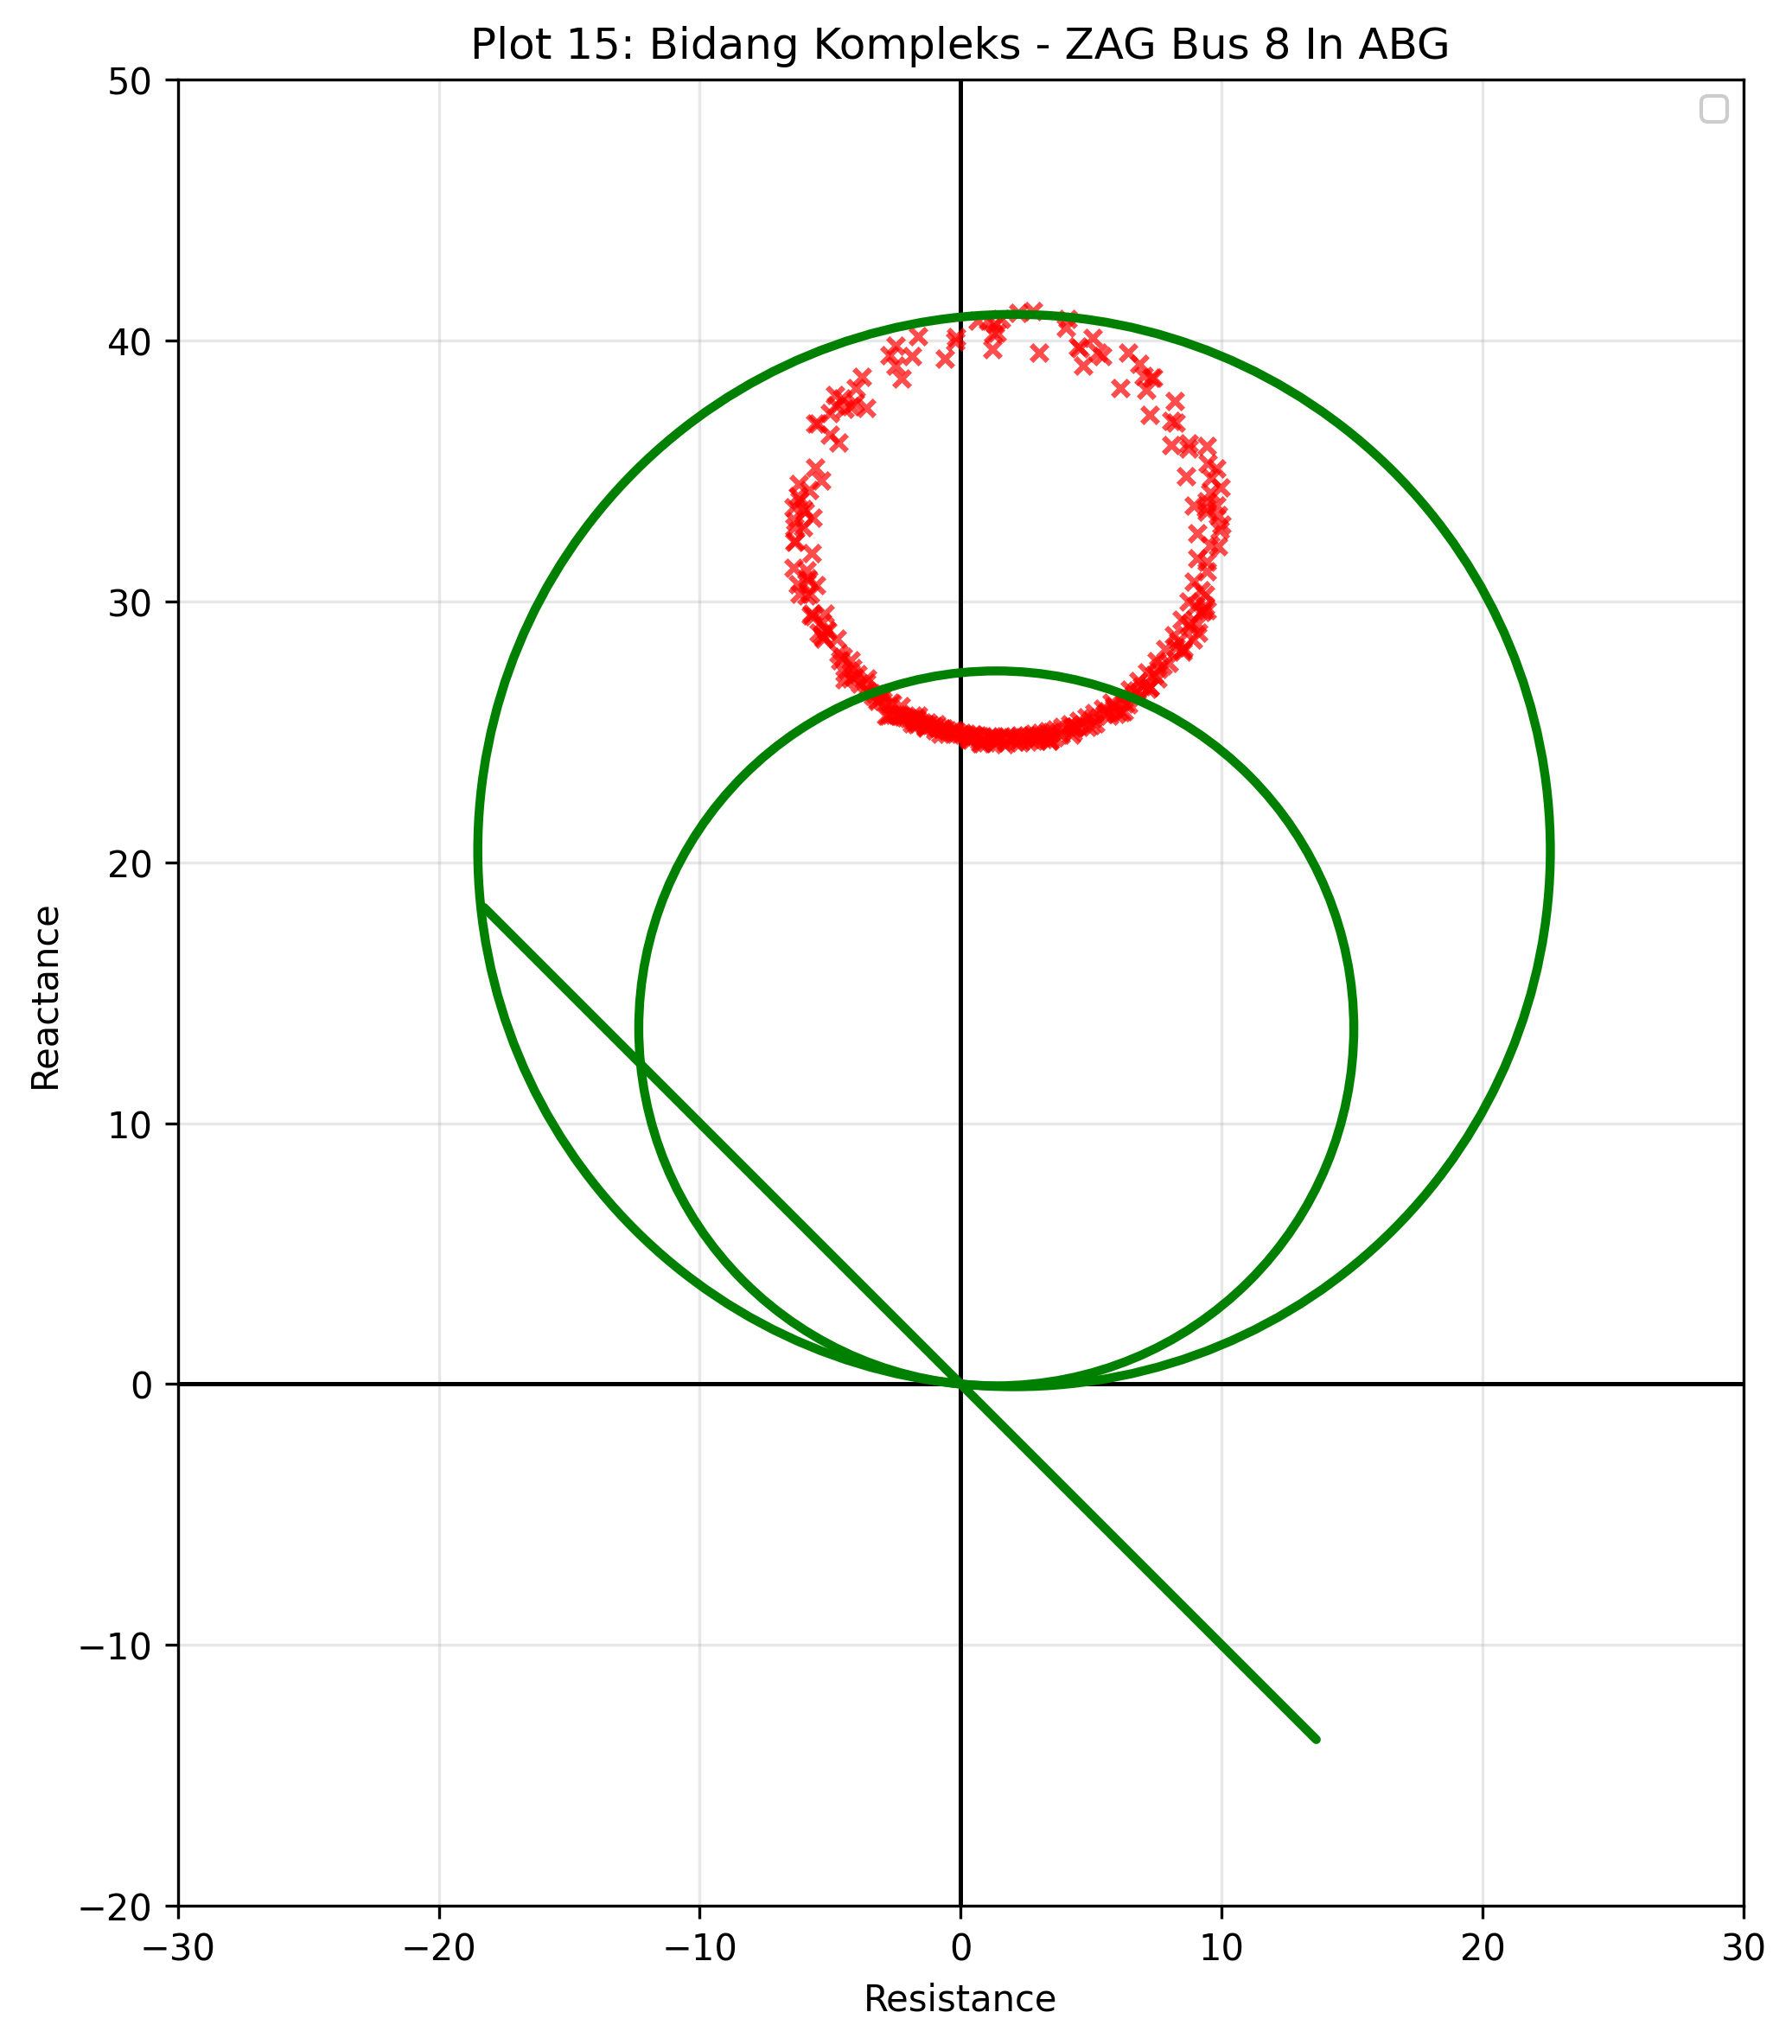
\includegraphics[width=0.8\textwidth]{contents/chapter-4/TIBR_15_ZAG_Bus_8_In_ABG.png}
    \caption{Impedansi Tampak ZAG Bus 8 Internal DLG Fault}
    \label{fig:TIBR_15_ZAG_Bus_8_In_ABG}
\end{figure}

Gambar \ref{fig:TIBR_15_ZAG_Bus_8_In_ABG} menunjukkan impedansi tampak loop fasa A dengan ground yang dibaca oleh relay 21 melalui CT dan VT pada Bus 8. Pada gangguan internal DLG, titik impedansi tampak yang terbaca masuk ke dalam zona 2. Kondisi tersebut menunjukkan bahwa relay 21 sisi Bus 8 mampu mendeteksi gangguan dan memberikan perintah trip kepada CB sesuai daerah operasi yang terbaca pada plot.

\begin{figure}[H]
    \centering
    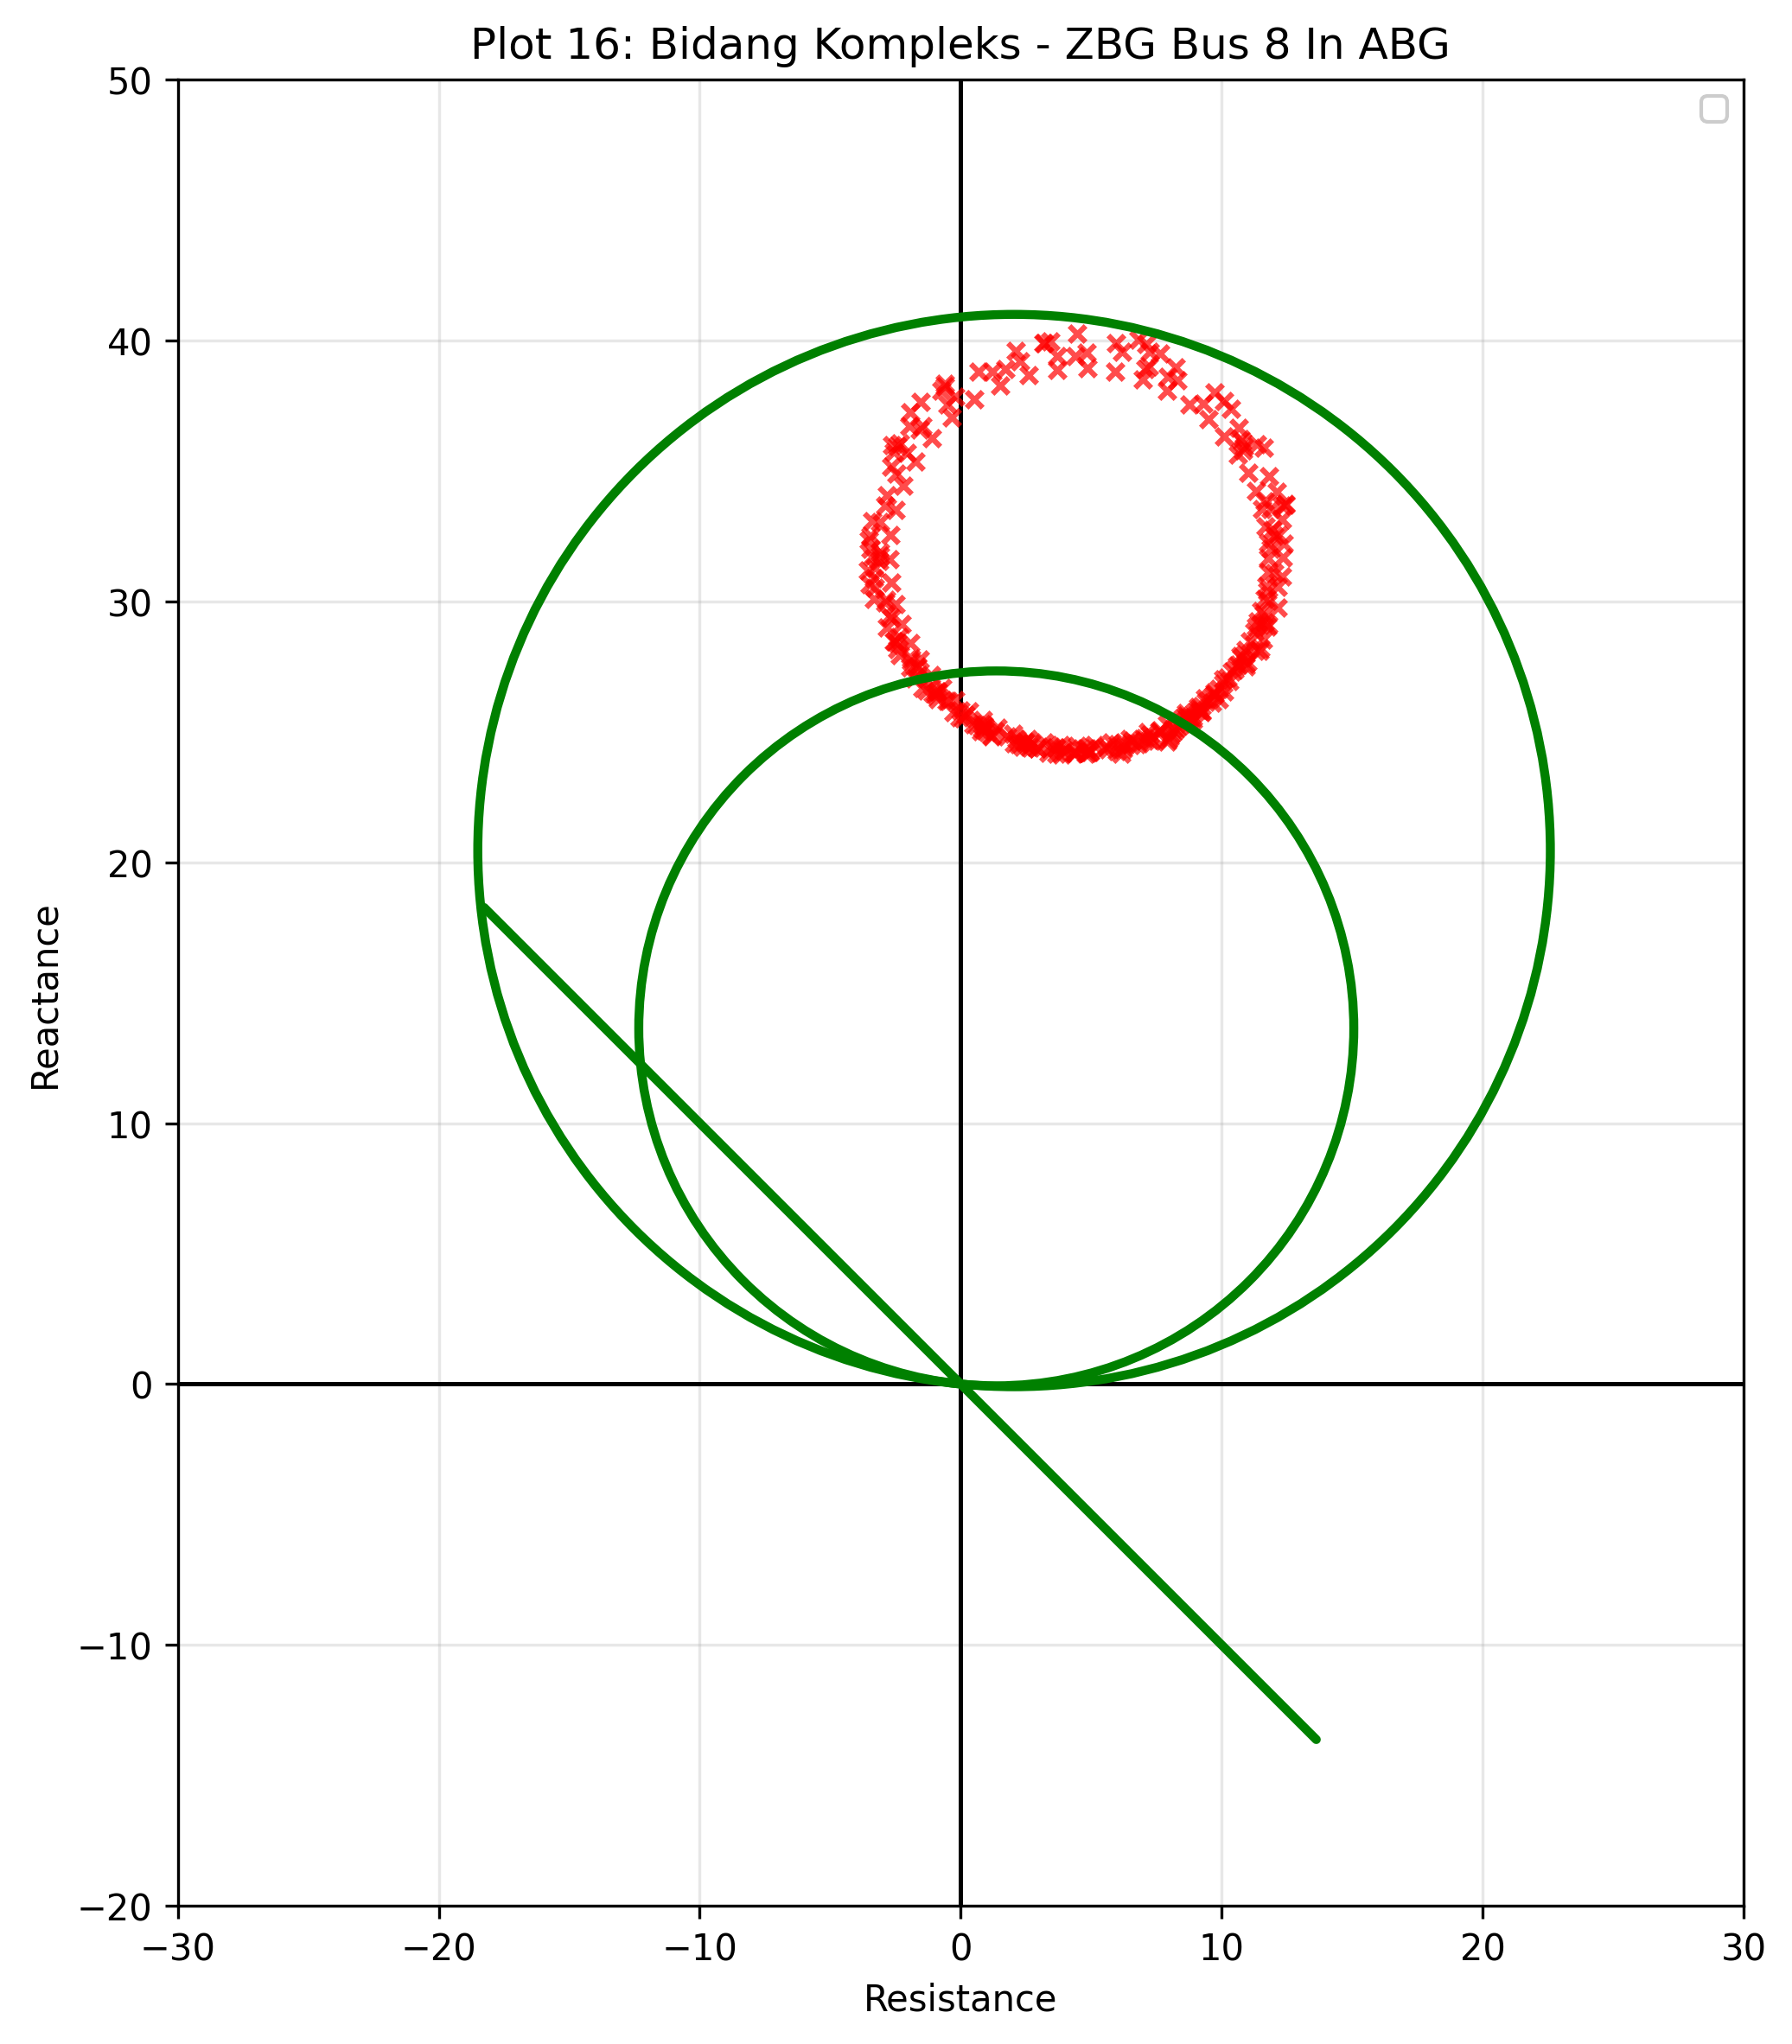
\includegraphics[width=0.8\textwidth]{contents/chapter-4/TIBR_16_ZBG_Bus_8_In_ABG.png}
    \caption{Impedansi Tampak ZBG Bus 8 Internal DLG Fault}
    \label{fig:TIBR_16_ZBG_Bus_8_In_ABG}
\end{figure}

Gambar \ref{fig:TIBR_16_ZBG_Bus_8_In_ABG} menunjukkan impedansi tampak loop fasa B dengan ground yang dibaca oleh relay 21 melalui CT dan VT pada Bus 8. Hasil plot memperlihatkan bahwa saat terjadi gangguan internal DLG, impedansi tampak yang dibaca relay berada di dalam zona 2. Dengan pembacaan tersebut, relay mendeteksi gangguan dan mengeluarkan perintah trip kepada CB, sehingga respons relay pada elemen ini masih sesuai dengan kondisi gangguan internal.

\begin{figure}[H]
    \centering
    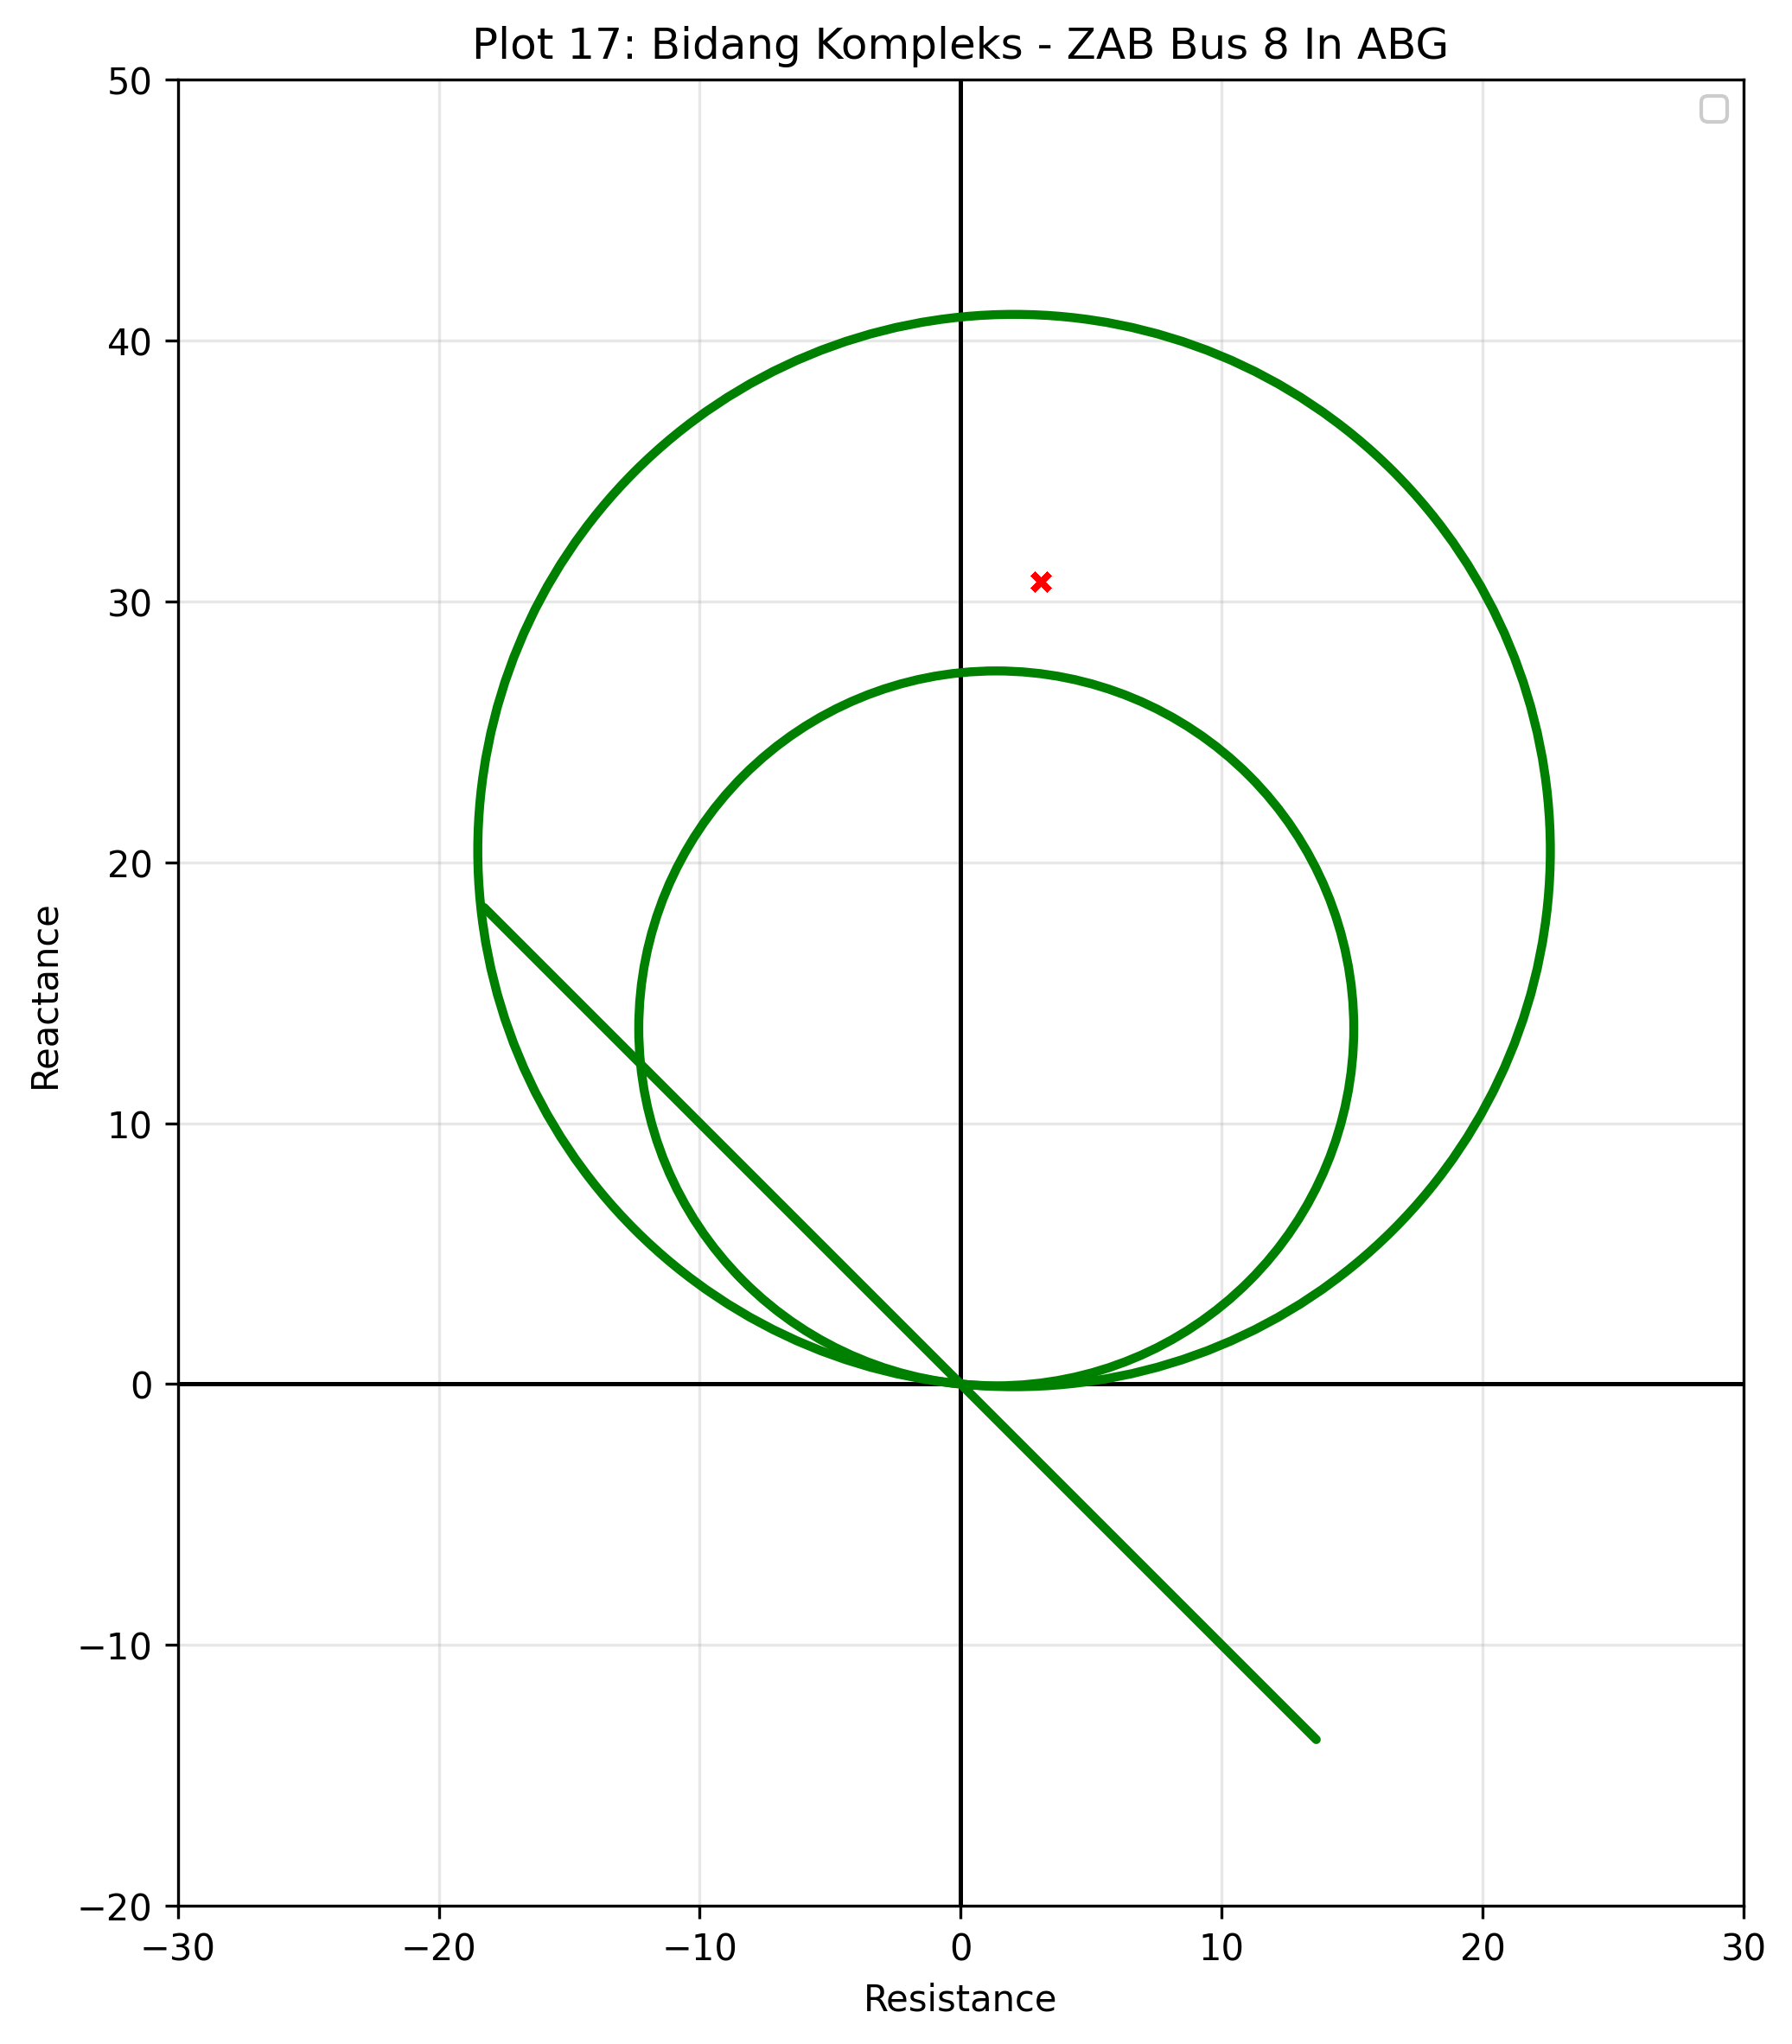
\includegraphics[width=0.8\textwidth]{contents/chapter-4/TIBR_17_ZAB_Bus_8_In_ABG.png}
    \caption{Impedansi Tampak ZAB Bus 8 Internal DLG Fault}
    \label{fig:TIBR_17_ZAB_Bus_8_In_ABG}
\end{figure}

Gambar \ref{fig:TIBR_17_ZAB_Bus_8_In_ABG} menunjukkan impedansi tampak loop fasa A dengan fasa B yang dibaca oleh relay 21 melalui CT dan VT pada Bus 8. Pada plot tersebut, titik impedansi tampak berada di dalam zona 2 ketika gangguan internal DLG terjadi. Hal ini menunjukkan bahwa relay 21 sisi Bus 8 masih membaca gangguan sebagai gangguan pada daerah operasinya dan memberikan perintah trip kepada CB.

\begin{figure}[H]
    \centering
    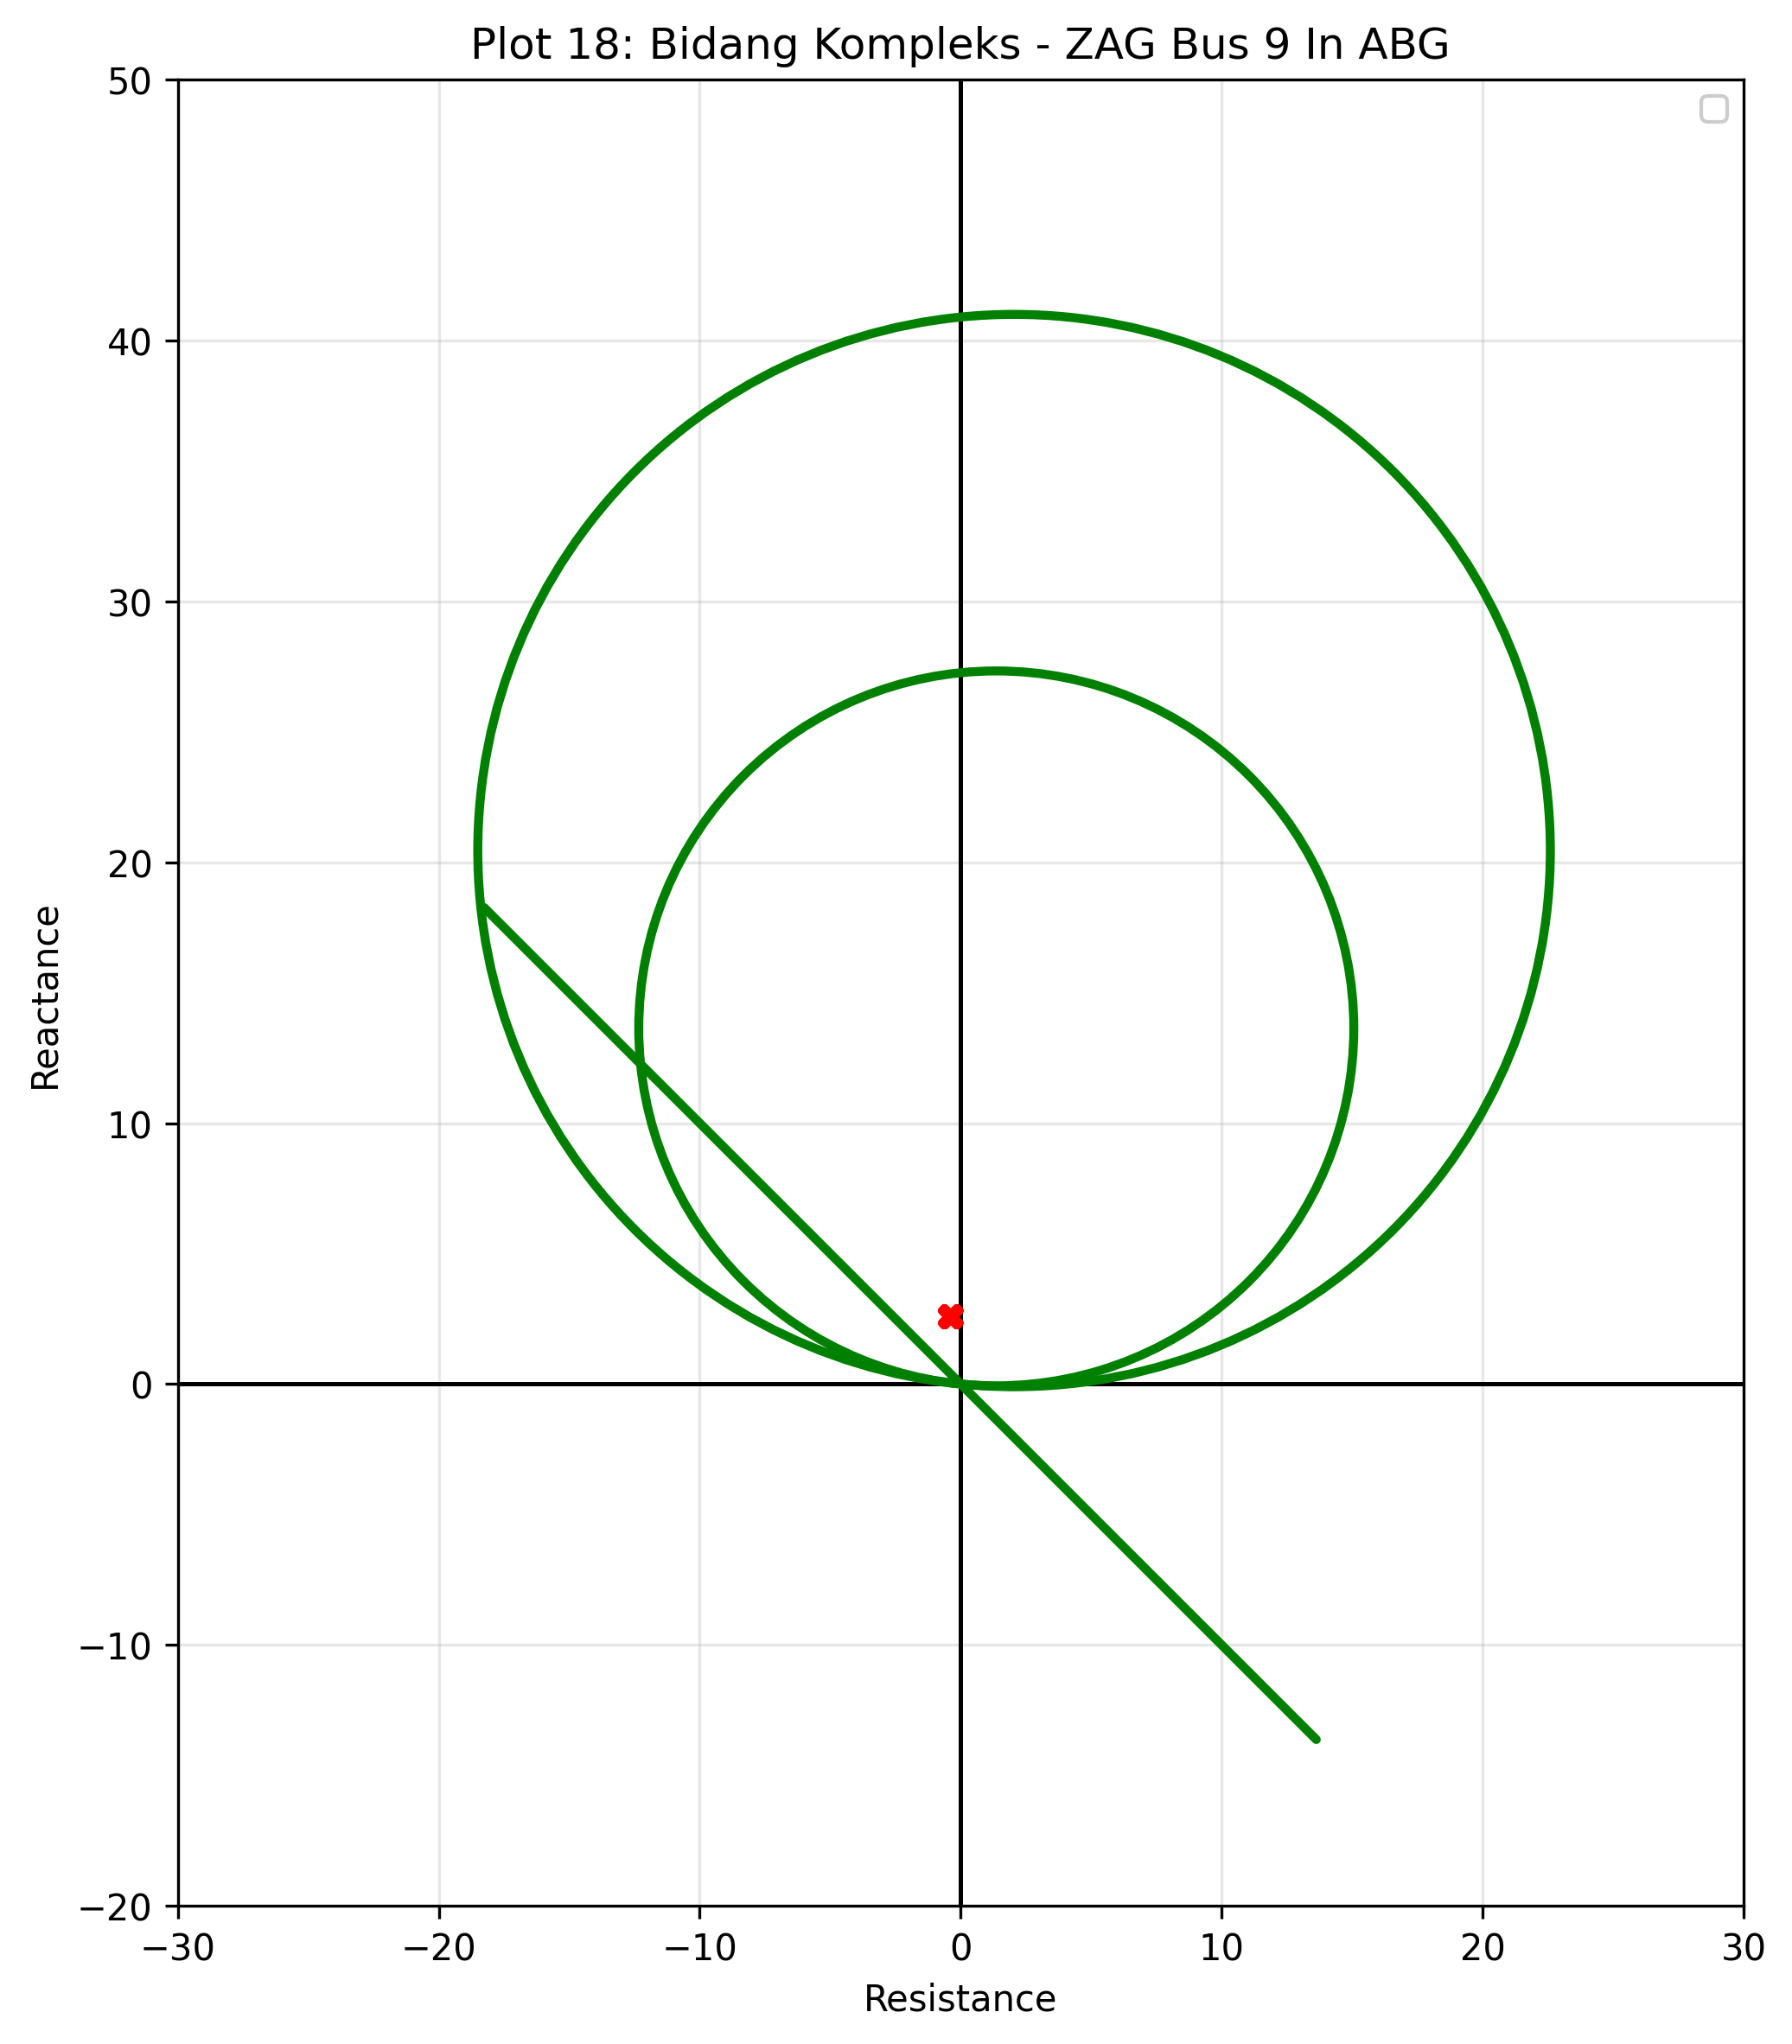
\includegraphics[width=0.8\textwidth]{contents/chapter-4/TIBR_18_ZAG_Bus_9_In_ABG.png}
    \caption{Impedansi Tampak ZAG Bus 9 Internal DLG Fault}
    \label{fig:TIBR_18_ZAG_Bus_9_In_ABG}
\end{figure}

Gambar \ref{fig:TIBR_18_ZAG_Bus_9_In_ABG} menunjukkan impedansi tampak loop fasa A dengan ground yang dibaca oleh relay 21 melalui CT dan VT pada Bus 9. Hasil plot menunjukkan bahwa saat terjadi gangguan internal DLG, impedansi tampak yang terbaca masuk ke dalam zona 1. Dengan posisi tersebut, relay 21 sisi Bus 9 mendeteksi adanya gangguan dan mengeluarkan perintah trip kepada CB.

\begin{figure}[H]
    \centering
    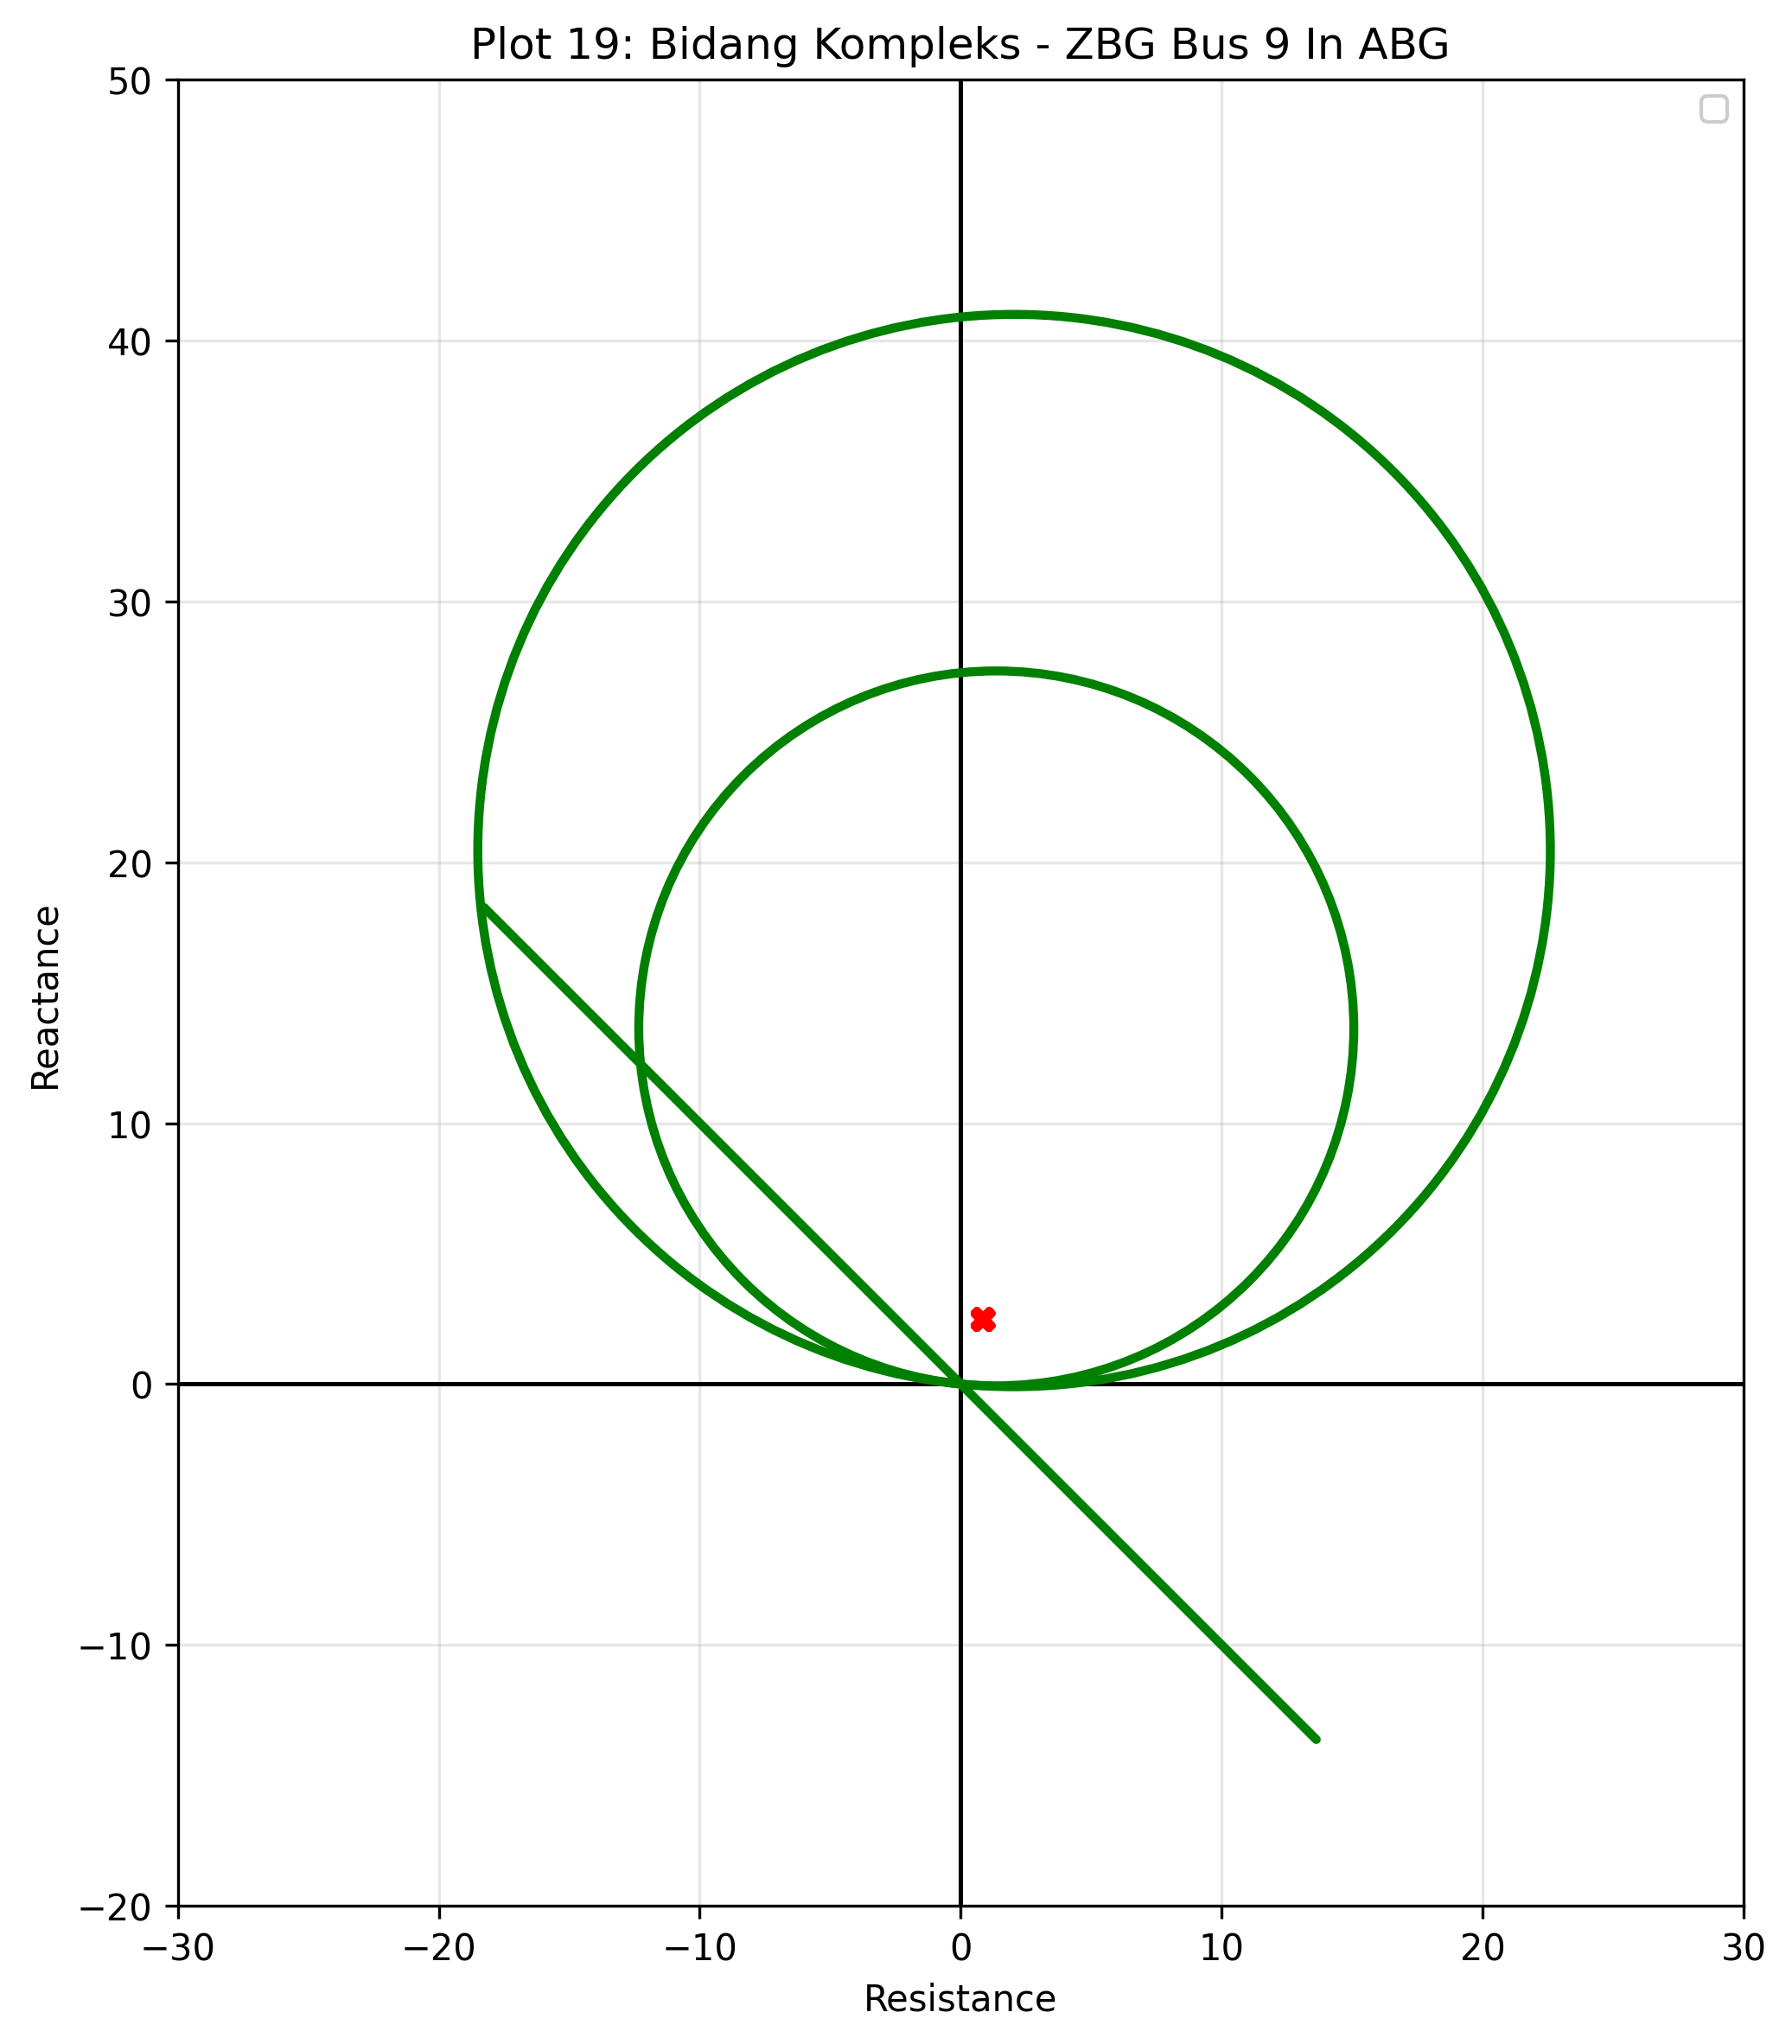
\includegraphics[width=0.8\textwidth]{contents/chapter-4/TIBR_19_ZBG_Bus_9_In_ABG.png}
    \caption{Impedansi Tampak ZBG Bus 9 Internal DLG Fault}
    \label{fig:TIBR_19_ZBG_Bus_9_In_ABG}
\end{figure}

Gambar \ref{fig:TIBR_19_ZBG_Bus_9_In_ABG} menunjukkan impedansi tampak loop fasa B dengan ground yang dibaca oleh relay 21 melalui CT dan VT pada Bus 9. Pada kondisi gangguan internal DLG, titik impedansi tampak berada di dalam zona 1. Hasil ini menunjukkan bahwa relay 21 sisi Bus 9 mengenali gangguan sebagai gangguan pada daerah operasinya dan memberikan perintah trip kepada CB.

\begin{figure}[H]
    \centering
    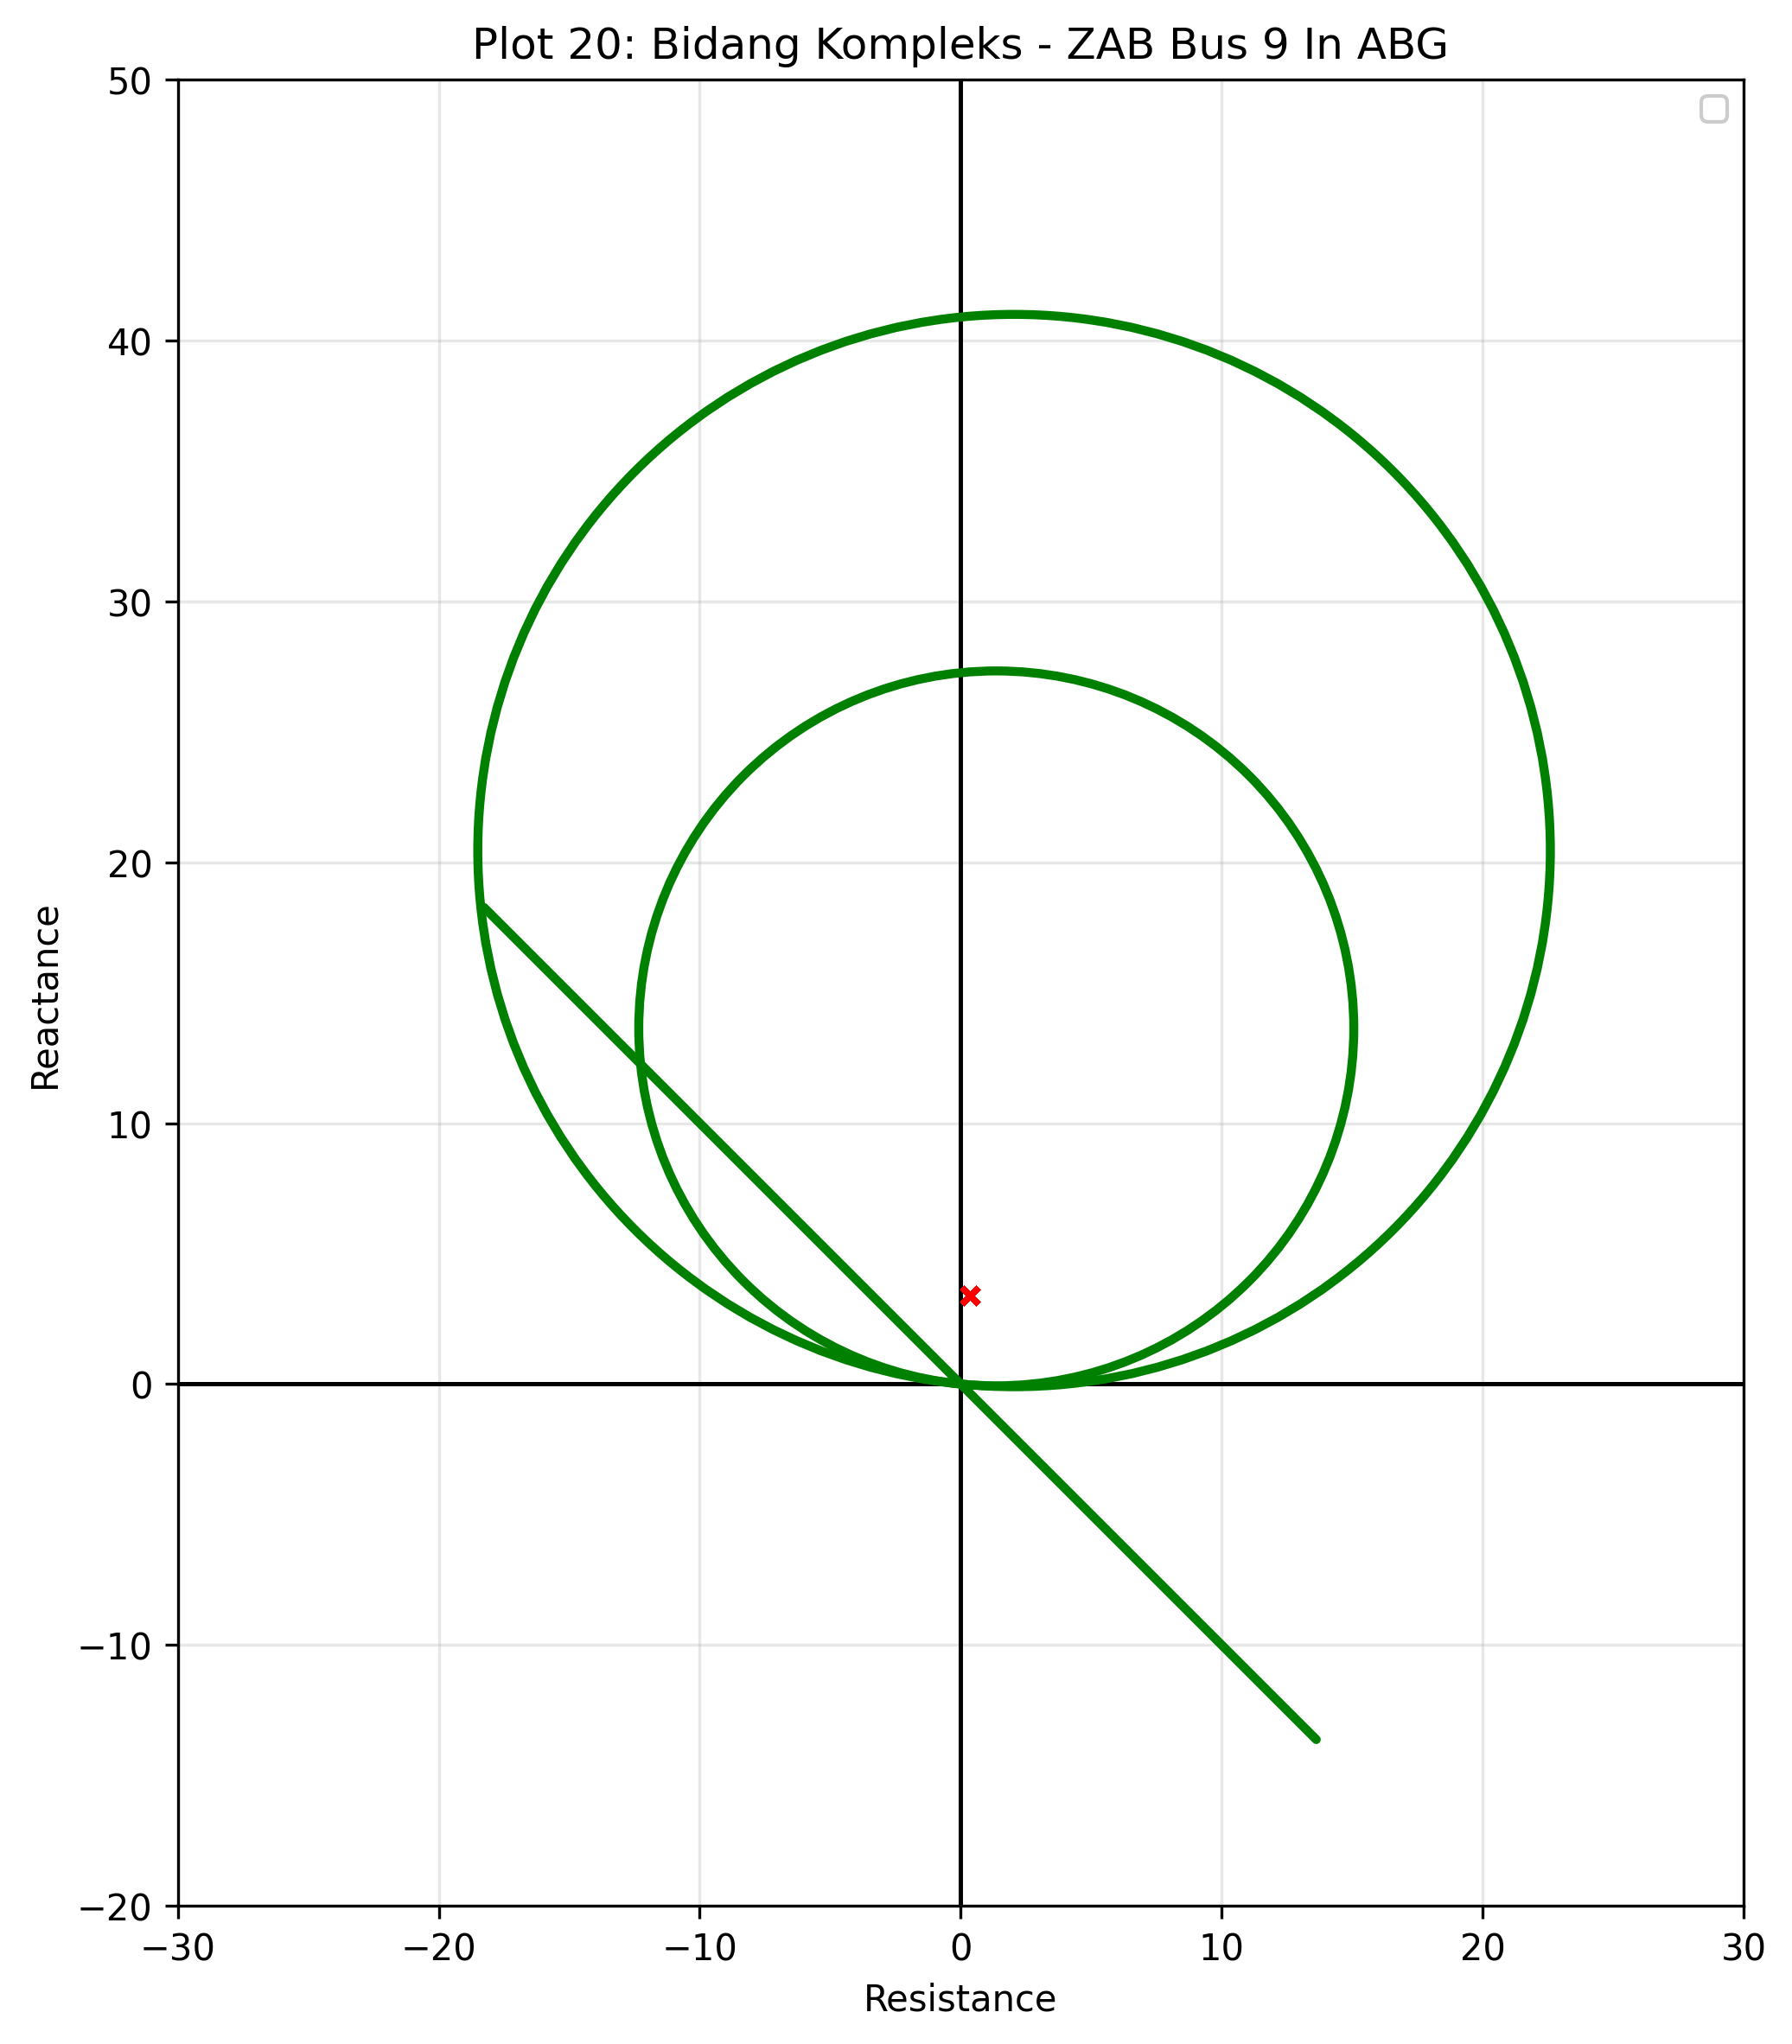
\includegraphics[width=0.8\textwidth]{contents/chapter-4/TIBR_20_ZAB_Bus_9_In_ABG.png}
    \caption{Impedansi Tampak ZAB Bus 9 Internal DLG Fault}
    \label{fig:TIBR_20_ZAB_Bus_9_In_ABG}
\end{figure}

Gambar \ref{fig:TIBR_20_ZAB_Bus_9_In_ABG} menunjukkan impedansi tampak loop fasa A dengan fasa B yang dibaca oleh relay 21 melalui CT dan VT pada Bus 9. Plot tersebut memperlihatkan bahwa impedansi tampak yang terbaca masuk ke dalam zona 1 saat terjadi gangguan internal DLG. Oleh karena itu, relay 21 sisi Bus 9 mendeteksi gangguan dan memberikan perintah trip kepada CB sesuai karakteristik zona yang terbaca.

\begin{figure}[H]
    \centering
    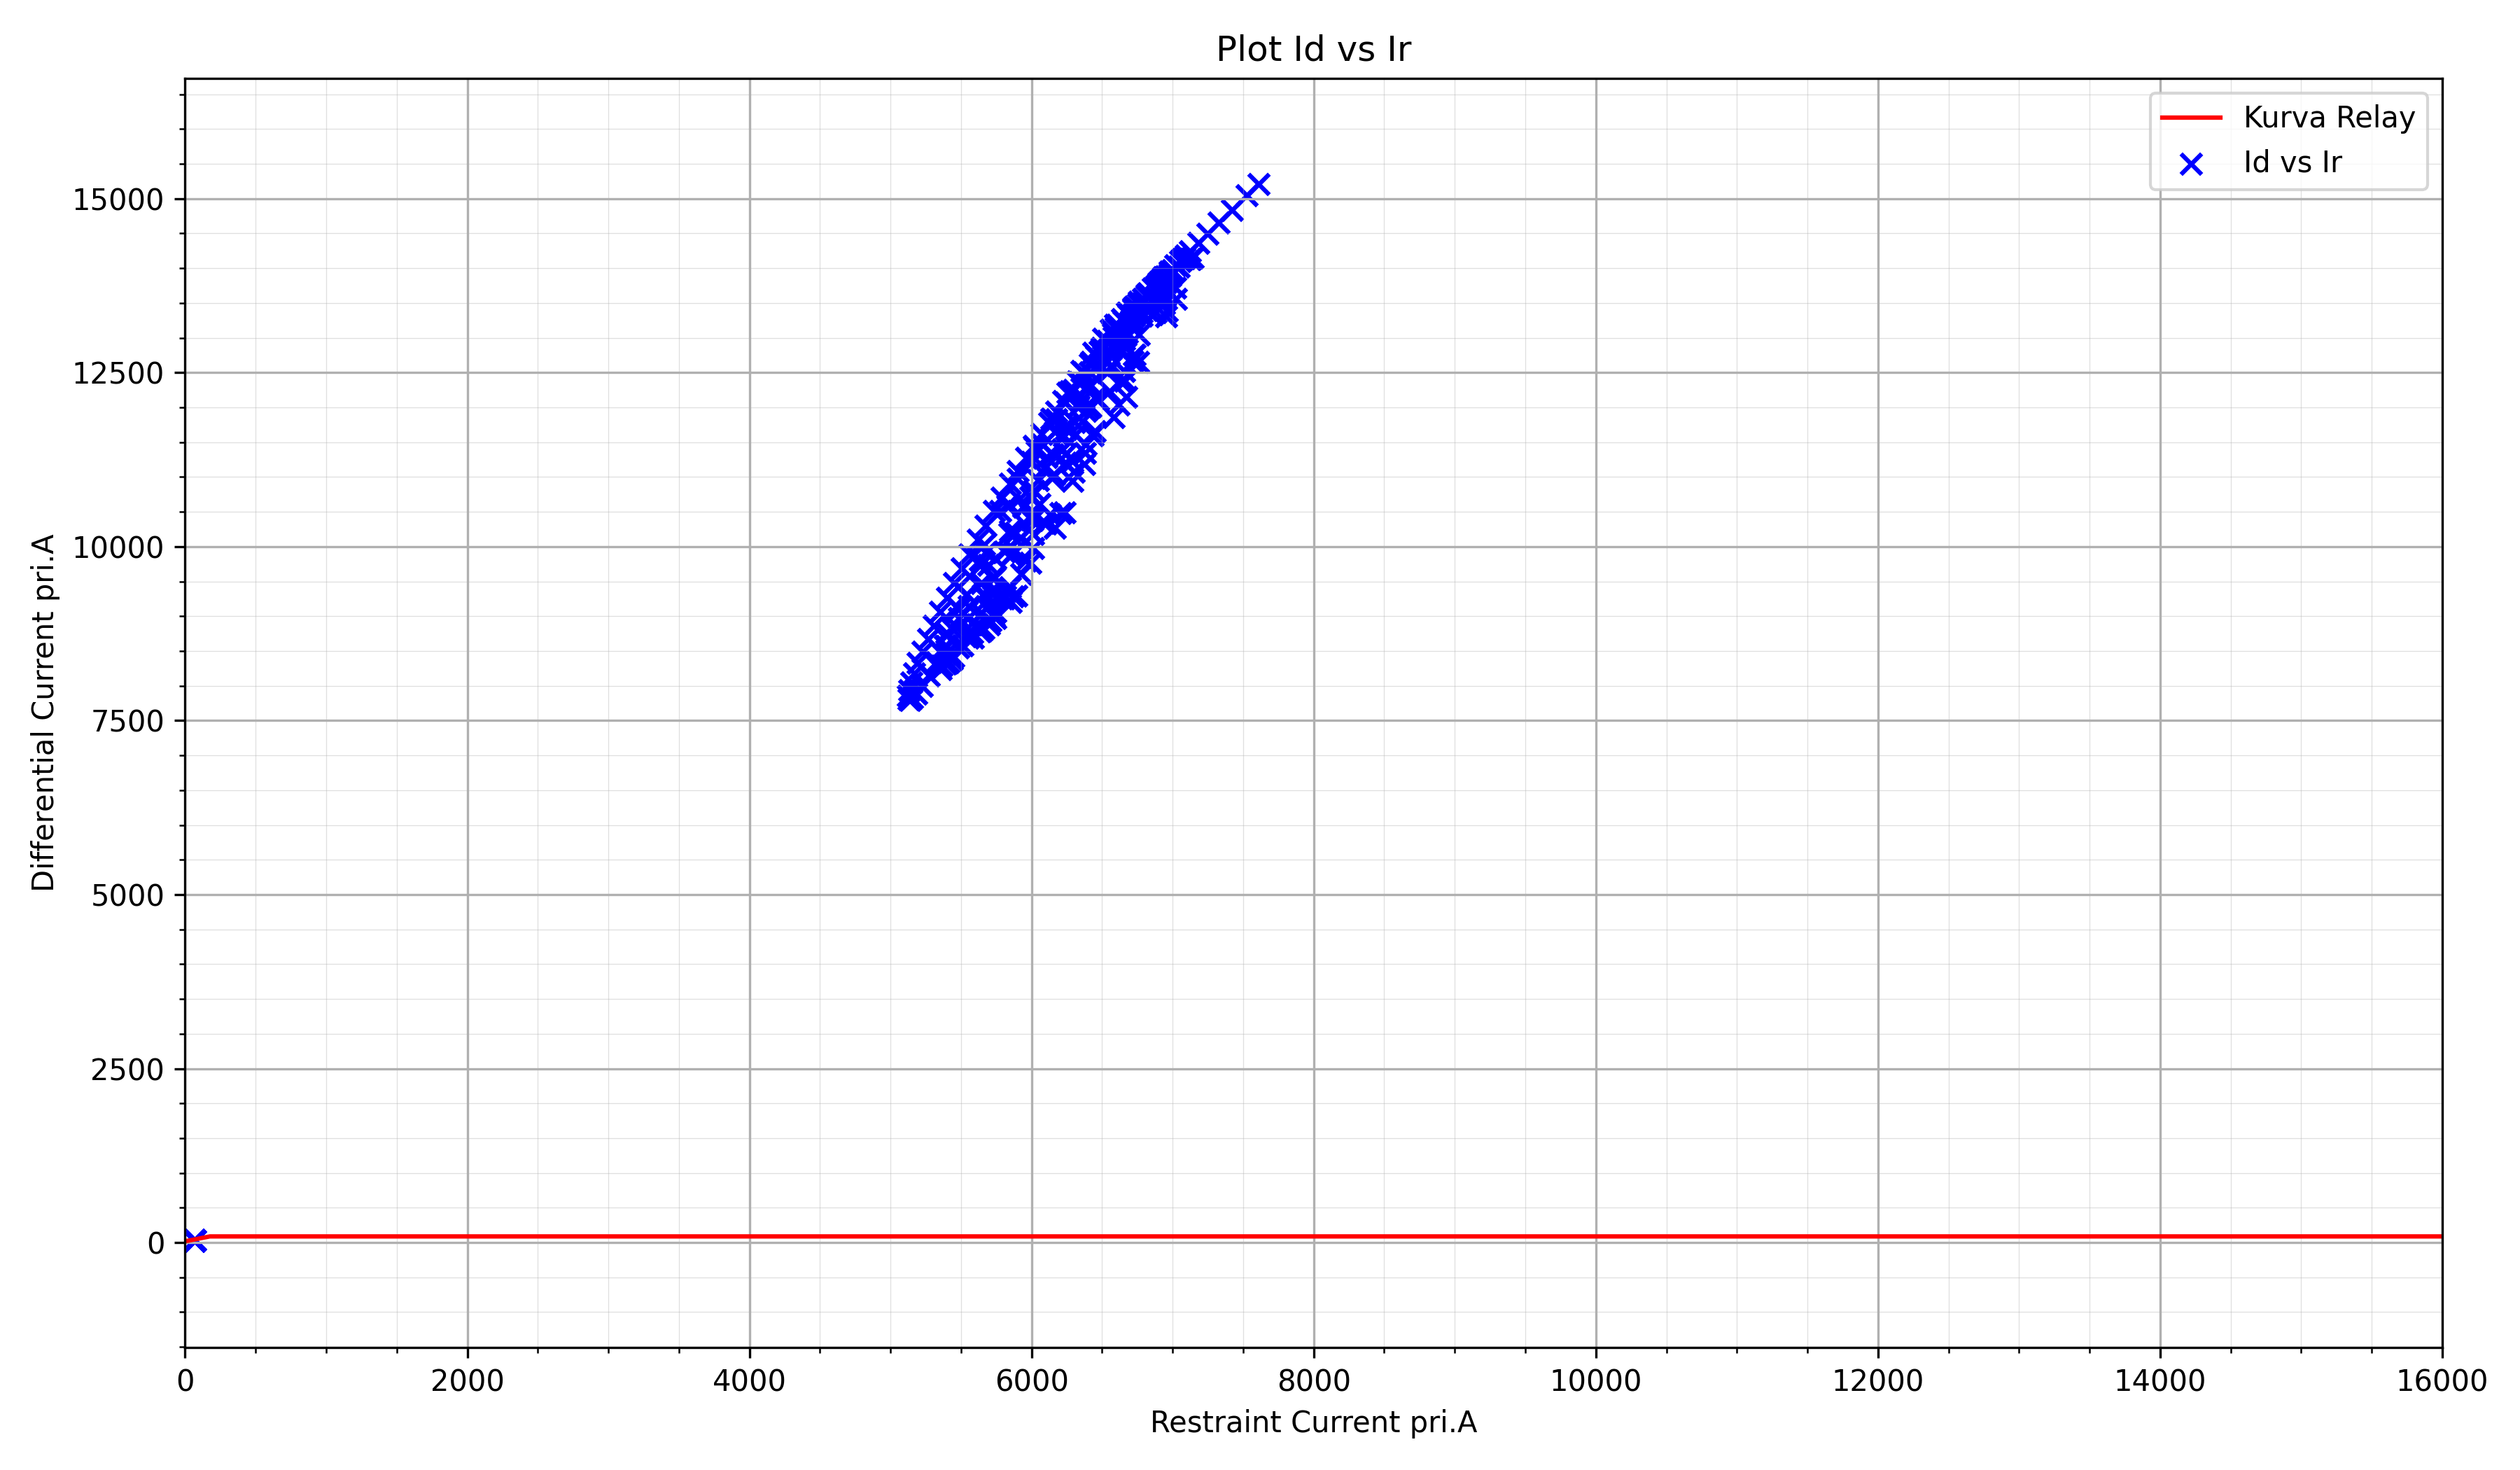
\includegraphics[width=0.8\textwidth]{contents/chapter-4/87LTIBR_plot_Ax4_Ay4.png}
    \caption{Current Comparison Differential Fasa A Internal DLG Fault}
    \label{fig:87LTIBR_plot_Ax4_Ay4}
\end{figure}

Gambar \ref{fig:87LTIBR_plot_Ax4_Ay4} menunjukkan plot \textit{current comparison differential} fasa A saat terjadi gangguan internal DLG. Titik arus pada plot berada di atas batas operasi yang ditentukan oleh setting relay. Posisi tersebut menyebabkan relay 87L membaca adanya gangguan dan memerintahkan trip pada CB, sehingga respons relay sesuai dengan kondisi gangguan yang berada di dalam daerah proteksi.

\begin{figure}[H]
    \centering
    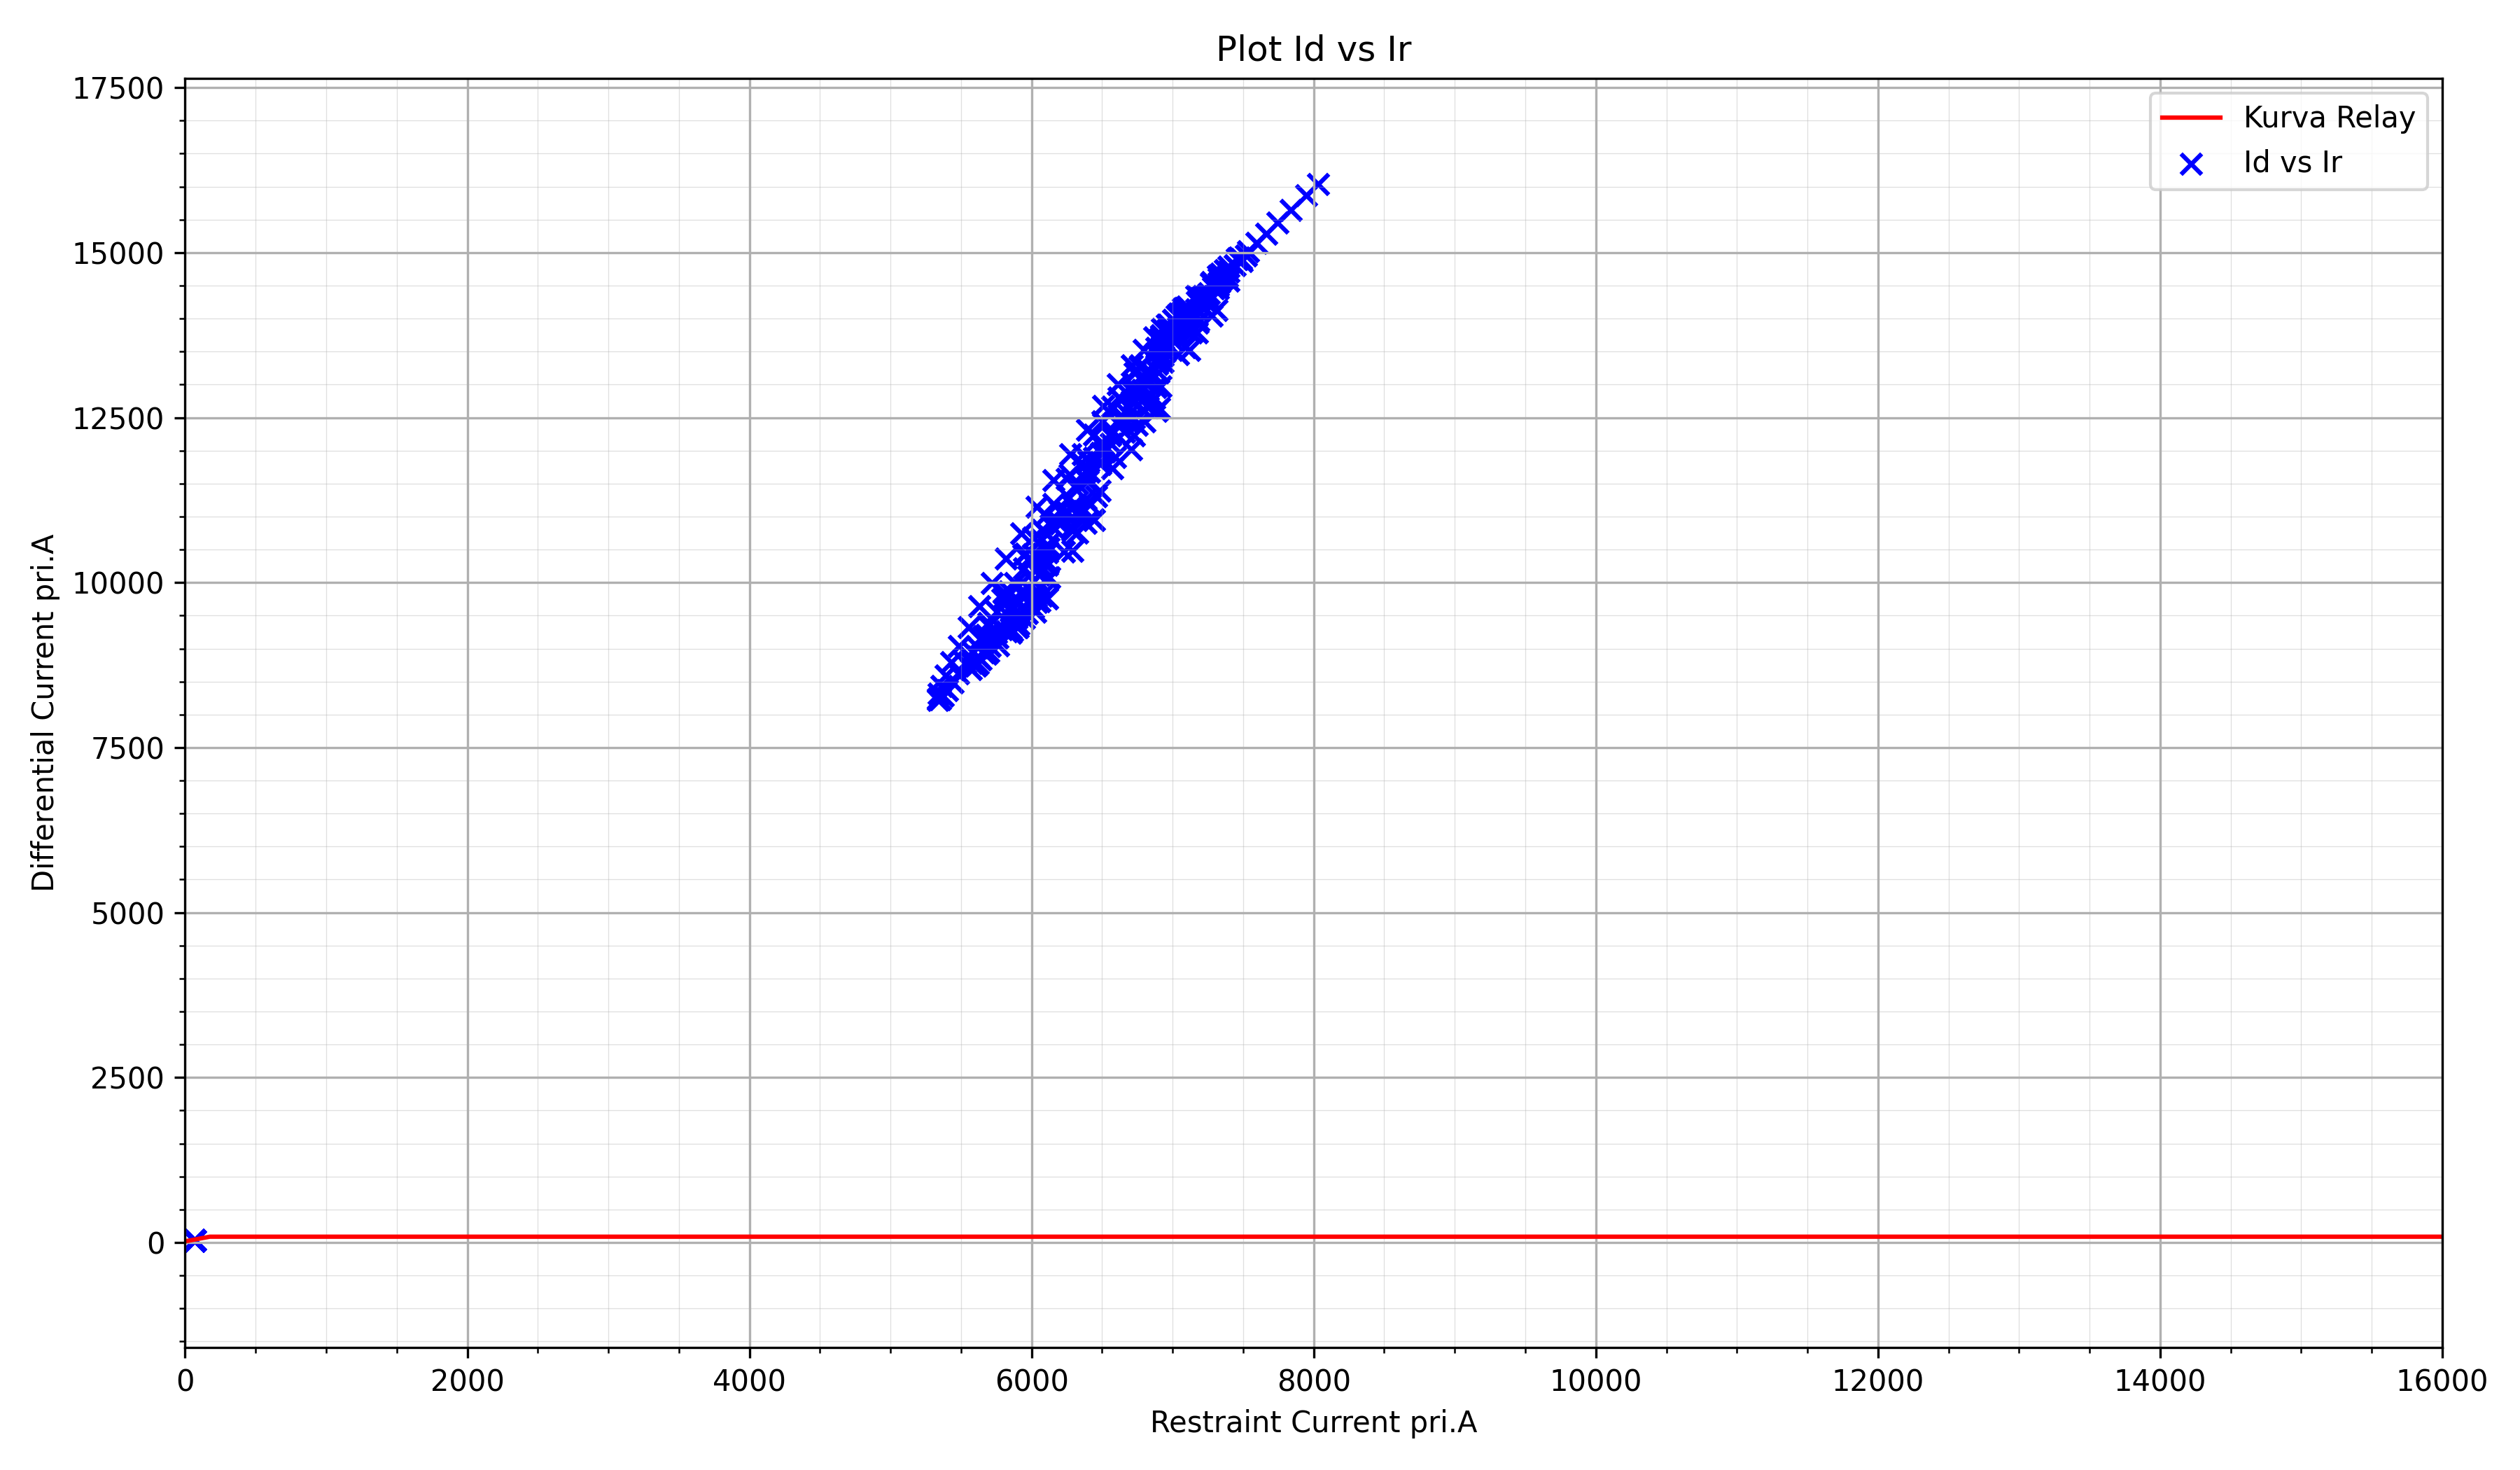
\includegraphics[width=0.8\textwidth]{contents/chapter-4/87LTIBR_plot_Bx4_By4.png}
    \caption{Current Comparison Differential Fasa B Internal DLG Fault}
    \label{fig:87LTIBR_plot_Bx4_By4}
\end{figure}

Gambar \ref{fig:87LTIBR_plot_Bx4_By4} menunjukkan plot \textit{current comparison differential} fasa B saat terjadi gangguan internal DLG. Sama seperti fasa A, titik arus pada fasa B berada di atas batas operasi yang ditentukan oleh setting relay. Dengan demikian, relay 87L membaca gangguan internal tersebut dan memberikan perintah trip kepada CB sebagai respons yang sesuai terhadap gangguan di daerah proteksi.

\begin{figure}[H]
    \centering
    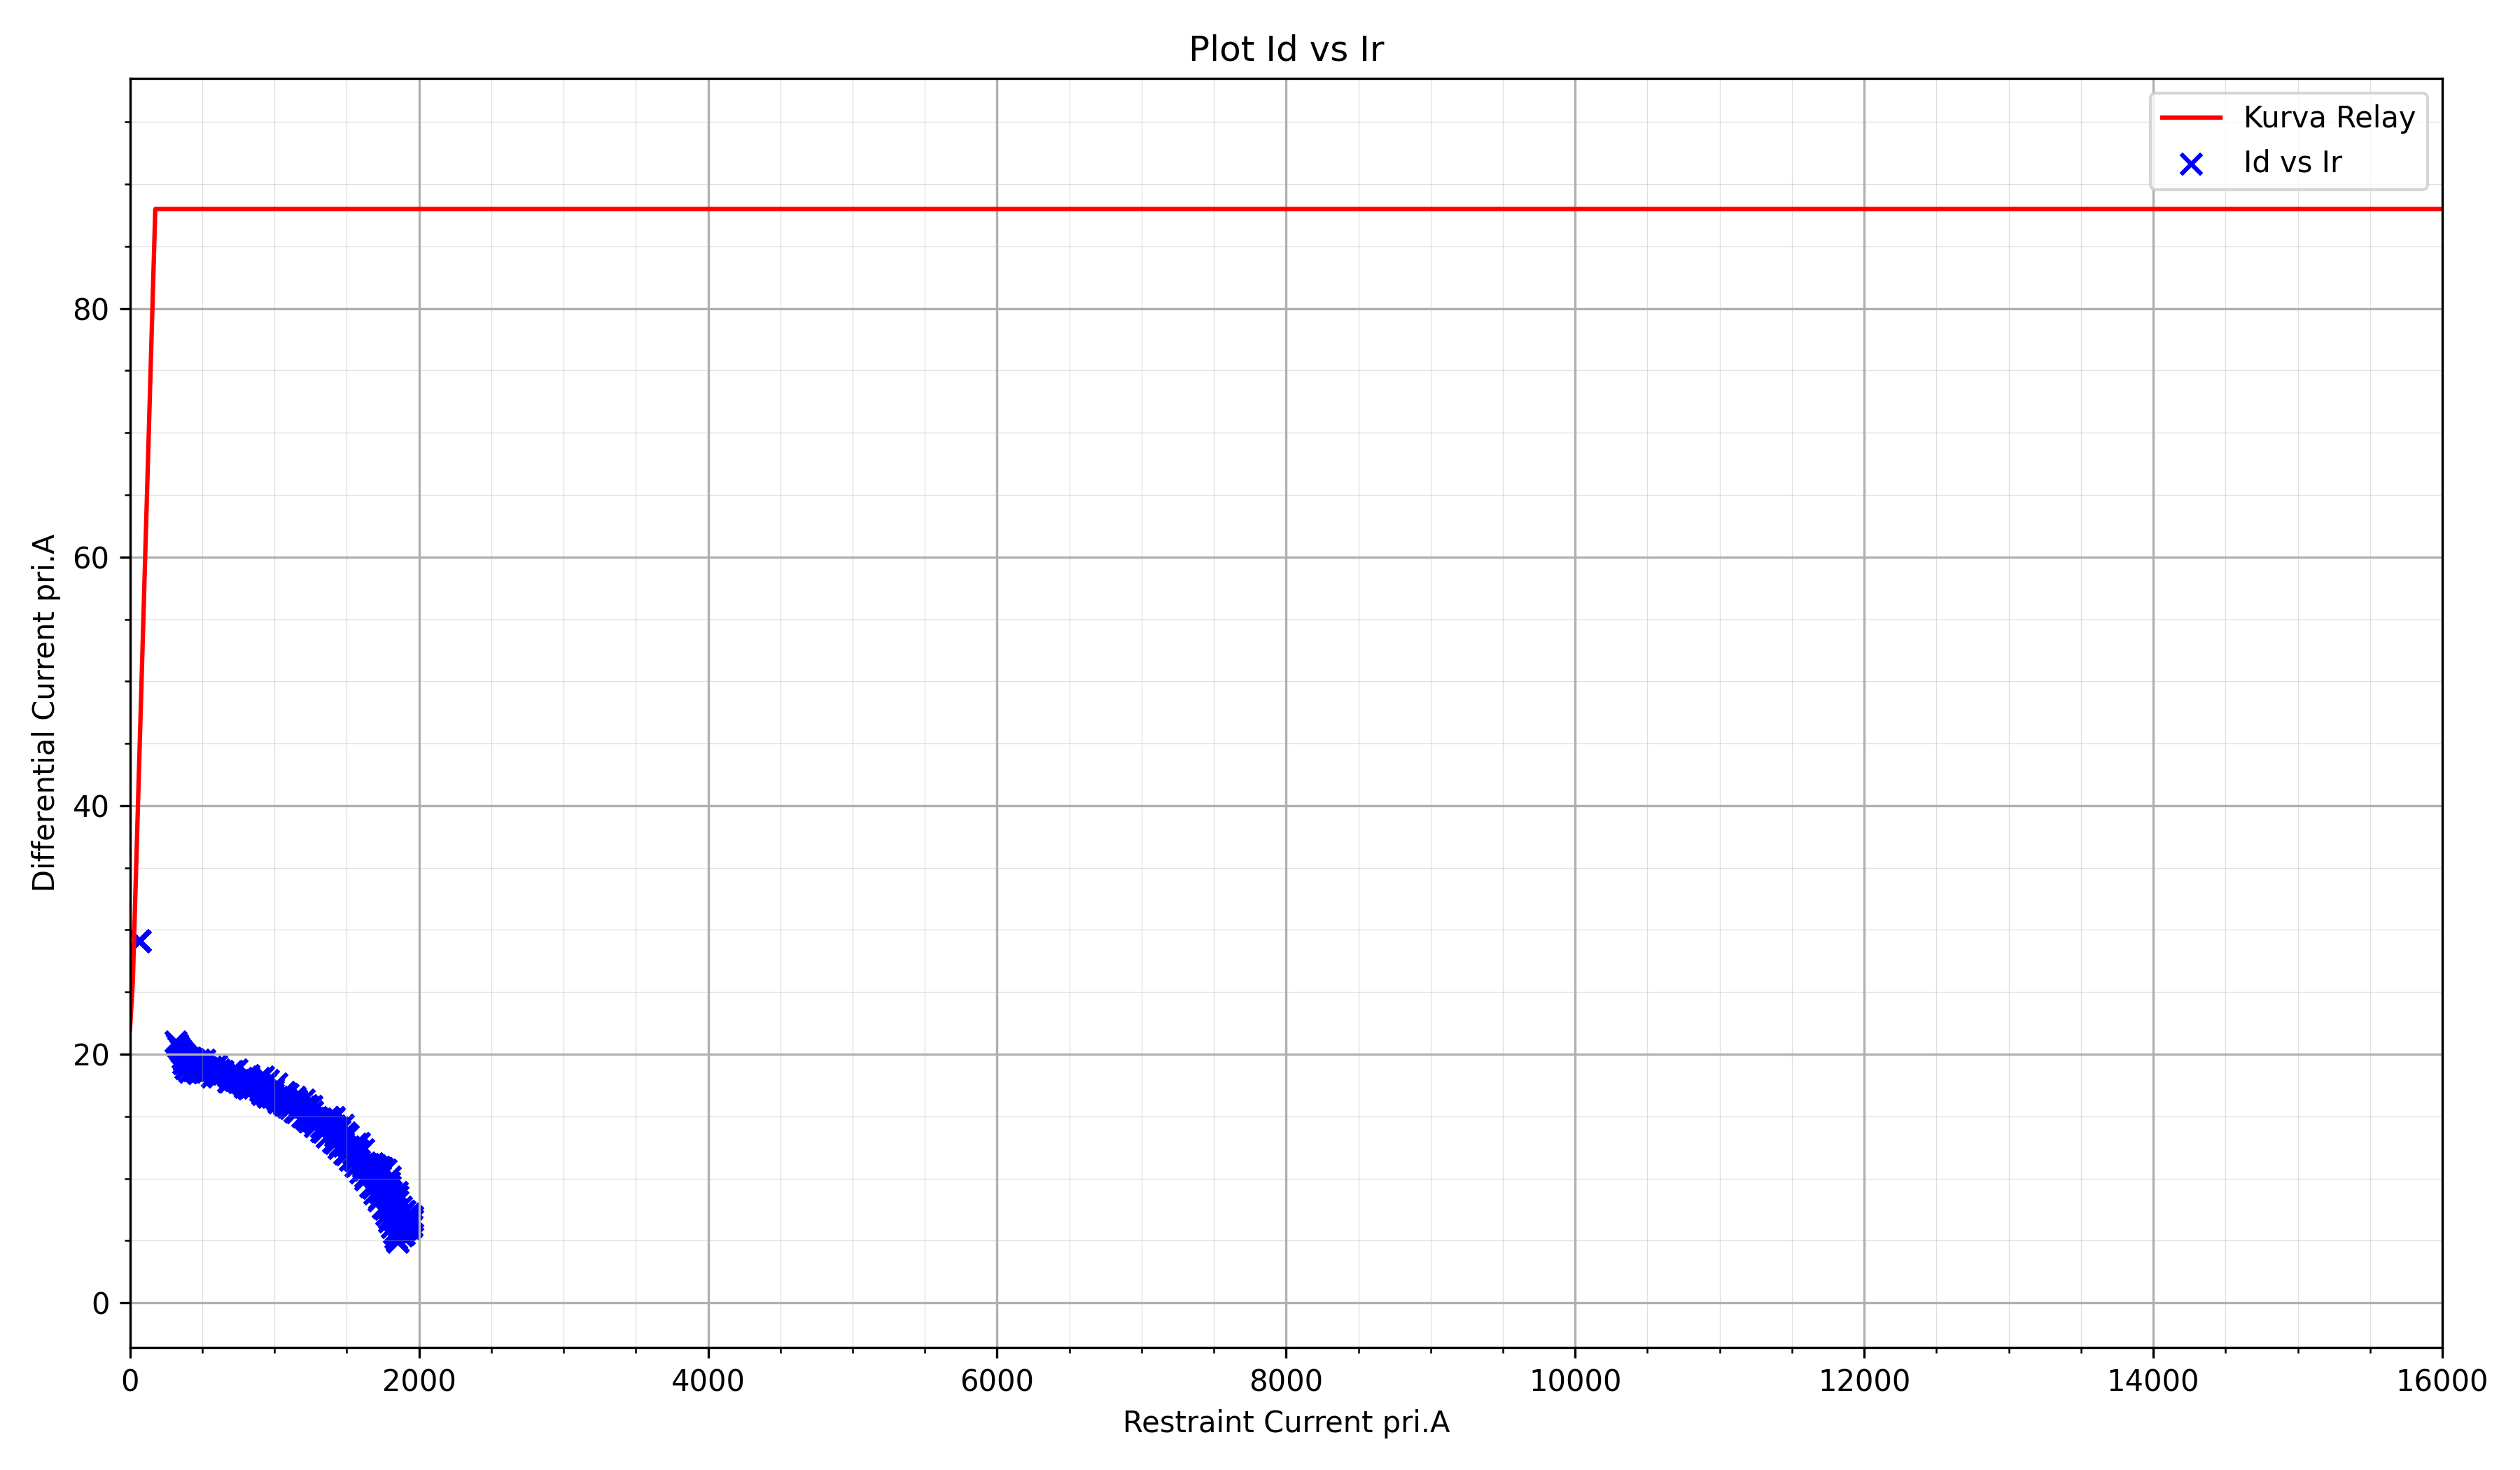
\includegraphics[width=0.8\textwidth]{contents/chapter-4/87LTIBR_plot_Cx4_Cy4.png}
    \caption{Current Comparison Differential Fasa C Internal DLG Fault}
    \label{fig:87LTIBR_plot_Cx4_Cy4}
\end{figure}

Gambar \ref{fig:87LTIBR_plot_Cx4_Cy4} menunjukkan plot \textit{current comparison differential} fasa C saat terjadi gangguan internal DLG. Pada fasa ini, titik arus berada di bawah batas operasi yang ditentukan oleh setting relay sehingga relay 87L tidak membaca adanya gangguan pada fasa C dan tidak mengeluarkan perintah trip dari fasa tersebut. Namun, keputusan operasi keseluruhan tetap terpenuhi karena fasa lain sudah berada pada daerah operasi dan telah memberikan perintah trip kepada CB.

\subsection{Respons Relay terhadap gangguan External 3 Phase}
\label{subsec:tanpa_IBR_ex_3p}

\begin{figure}[H]
    \centering
    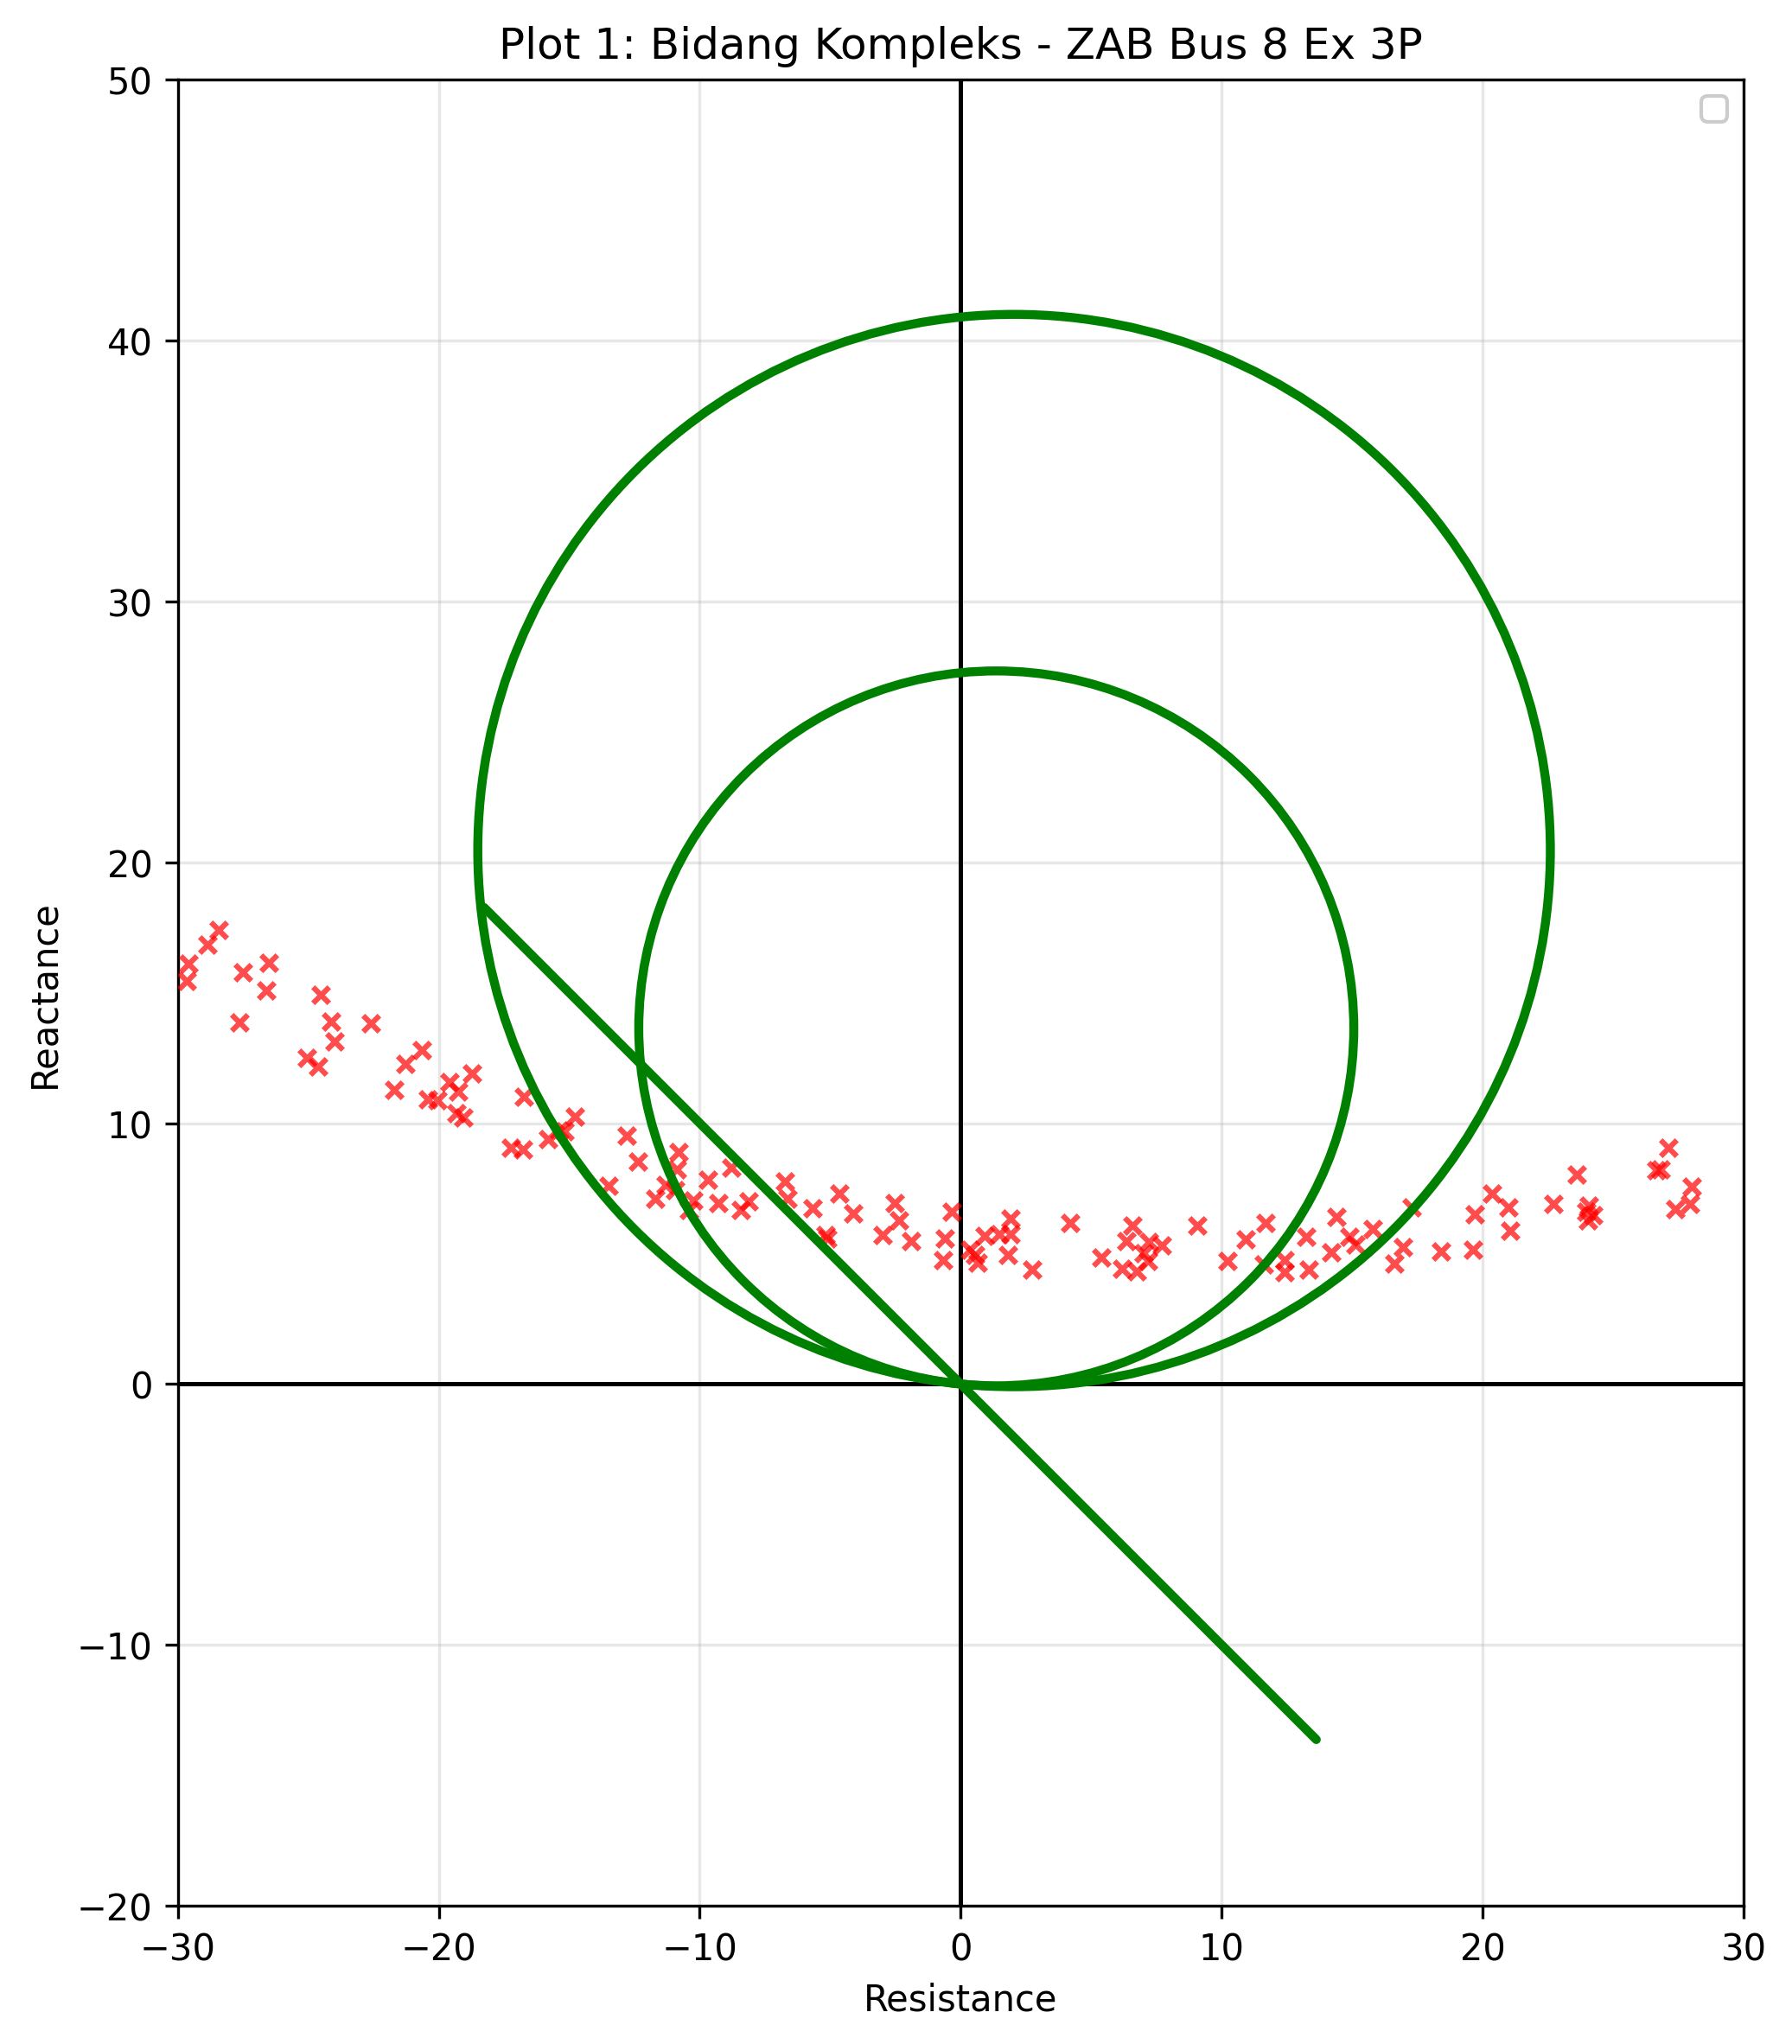
\includegraphics[width=0.8\textwidth]{contents/chapter-4/TIBR_01_ZAB_Bus_8_Ex_3P.png}
    \caption{Impedansi Tampak ZAB Bus 8 External 3P Fault}
    \label{fig:TIBR_01_ZAB_Bus_8_Ex_3P}
\end{figure}

\begin{figure}[H]
    \centering
    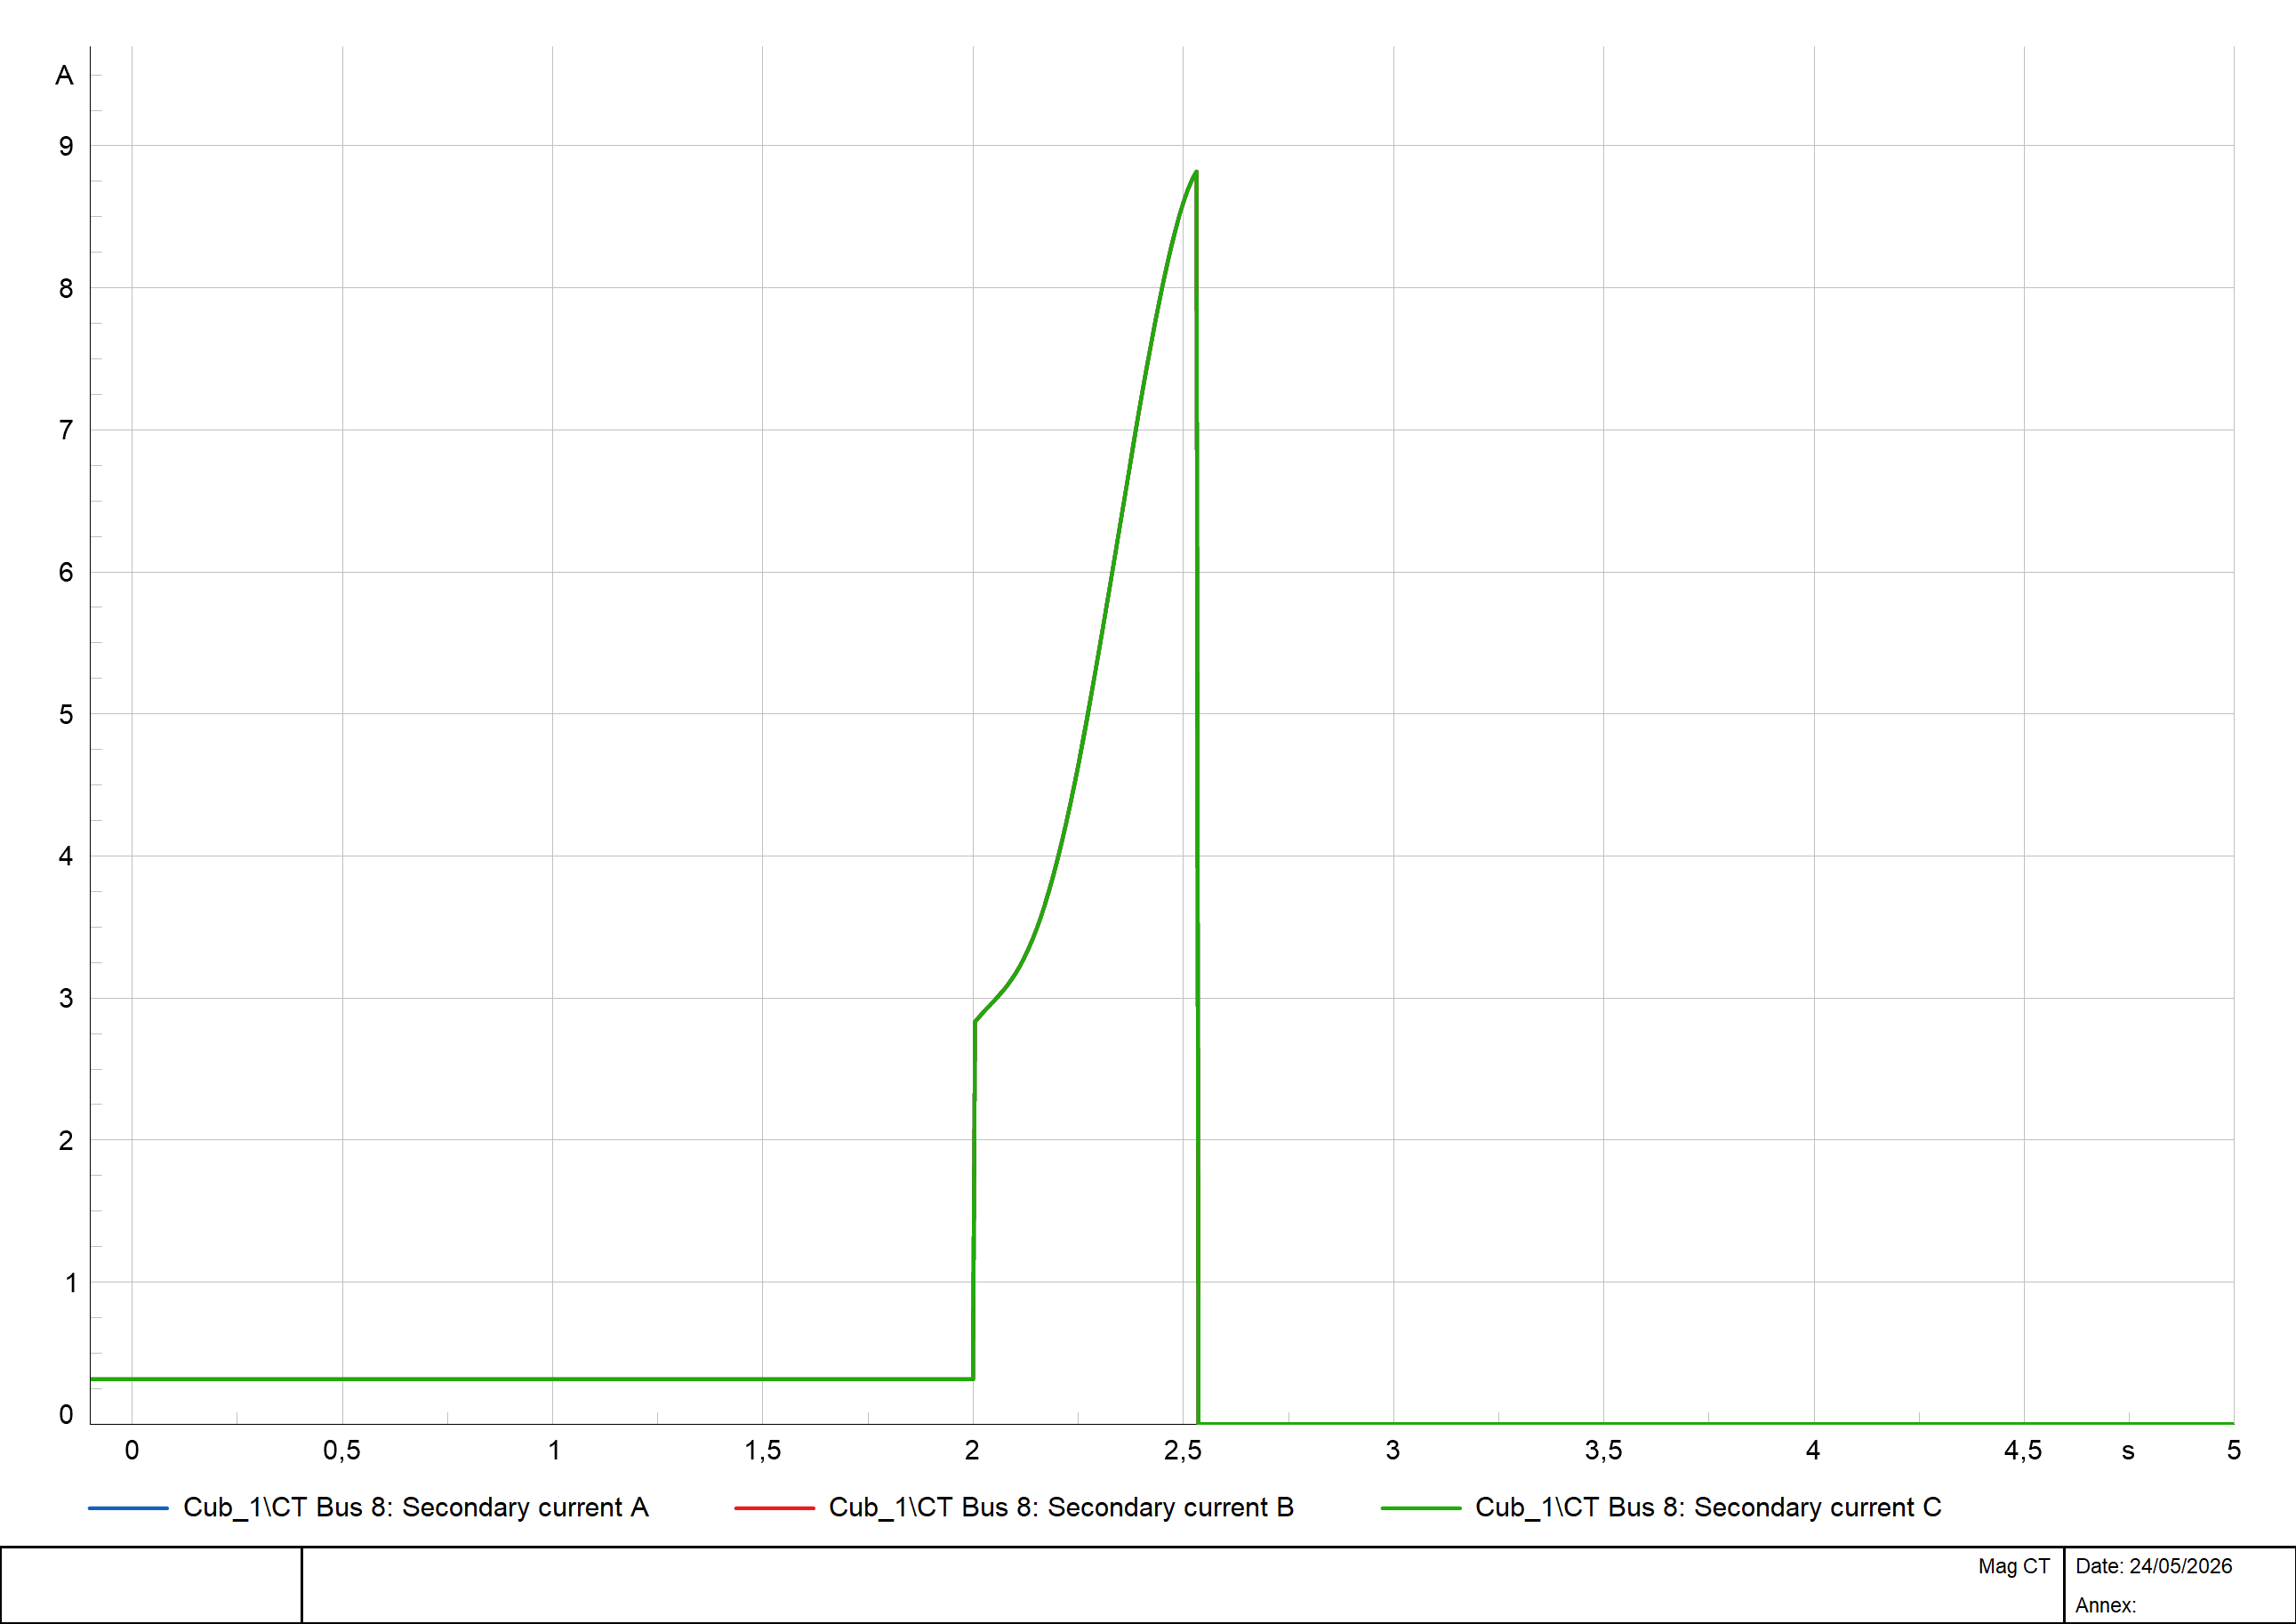
\includegraphics[width=0.8\textwidth]{contents/chapter-4/Bus_8_Ex_3P.png}
    \caption{Arus Sekunder CT Bus 8 External 3P Fault}
    \label{fig:Bus_8_Ex_3P}
\end{figure}

Gambar \ref{fig:TIBR_01_ZAB_Bus_8_Ex_3P} menunjukkan impedansi tampak elemen fasa A ke fasa B pada relay 21 sisi Bus 8 saat terjadi gangguan eksternal tiga fasa. Titik impedansi tampak sempat mengalami \textit{overreach} terhadap zona 1. Meskipun demikian, relay tetap memberikan perintah trip karena arus yang terbaca mencapai batas maksimum untuk \textit{instant trip}, sebagaimana ditunjukkan pada Gambar \ref{fig:Bus_8_Ex_3P}.

\begin{figure}[H]
    \centering
    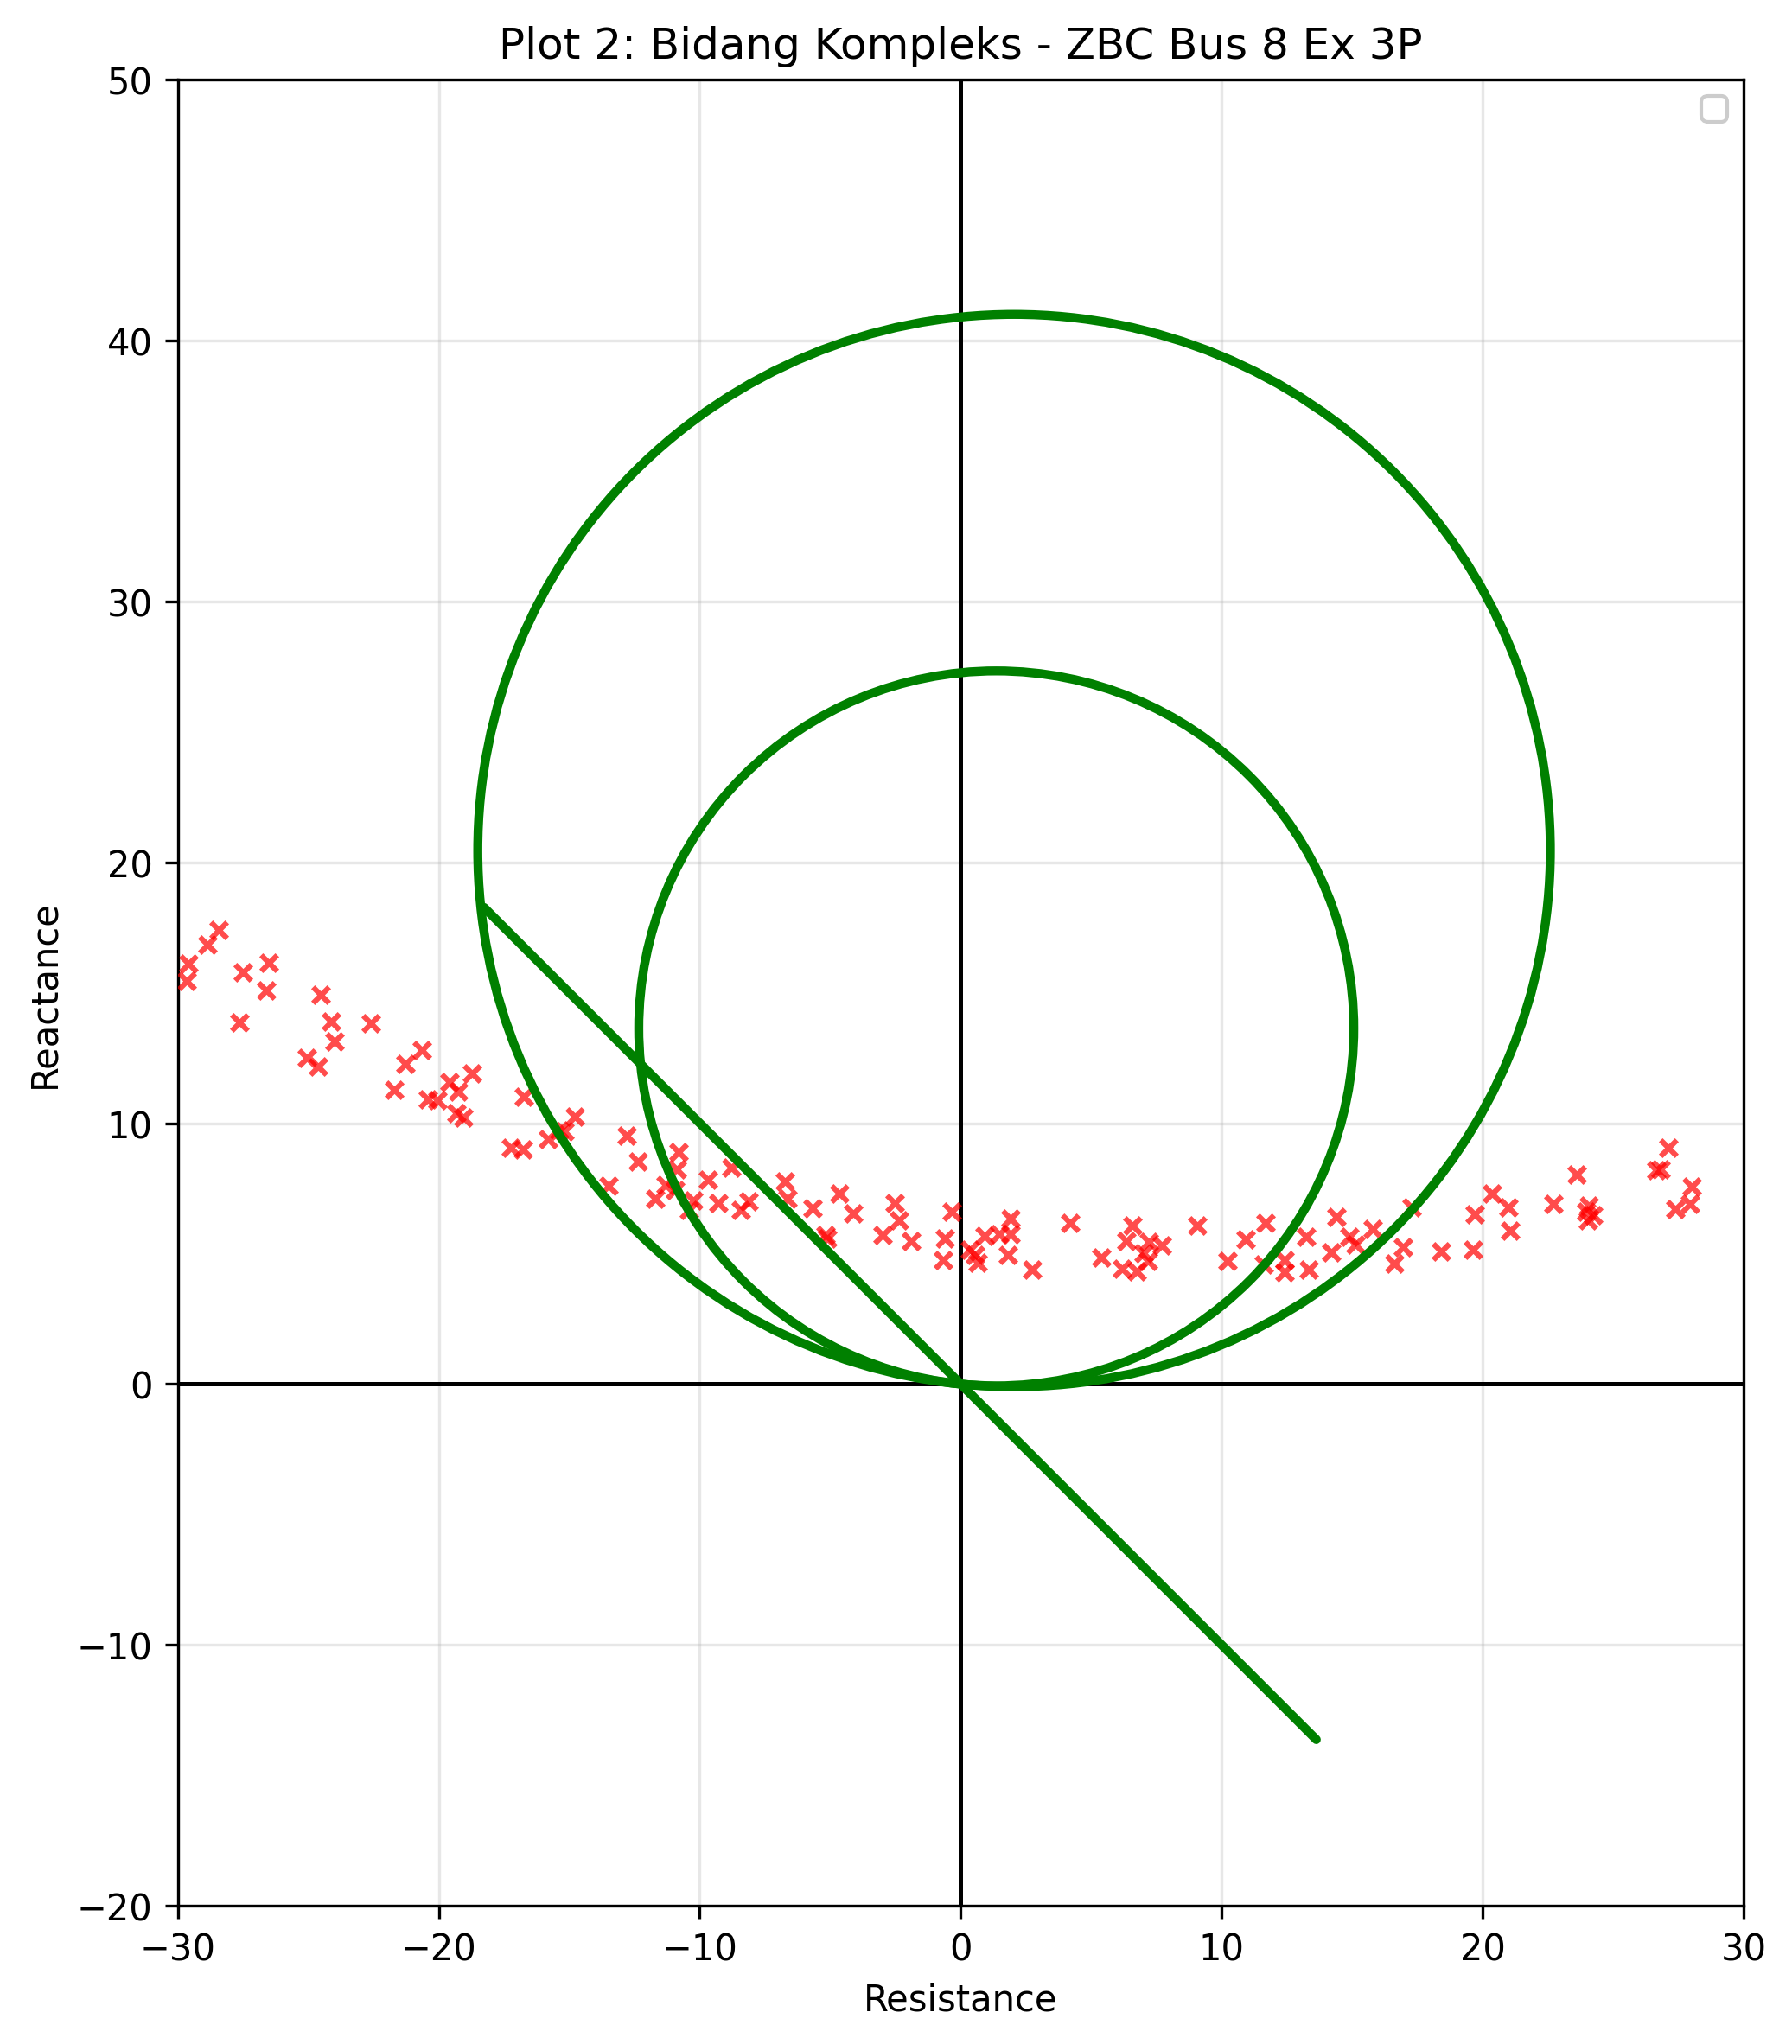
\includegraphics[width=0.8\textwidth]{contents/chapter-4/TIBR_02_ZBC_Bus_8_Ex_3P.png}
    \caption{Impedansi Tampak ZBC Bus 8 External 3P Fault}
    \label{fig:TIBR_02_ZBC_Bus_8_Ex_3P}
\end{figure}

Gambar \ref{fig:TIBR_02_ZBC_Bus_8_Ex_3P} menunjukkan impedansi tampak elemen fasa B ke fasa C pada relay 21 sisi Bus 8 saat terjadi gangguan eksternal tiga fasa. Pada plot tersebut, titik impedansi tampak juga sempat mengalami \textit{overreach} terhadap zona 1. Keputusan trip tetap muncul karena arus yang mengalir mencapai batas maksimum untuk \textit{instant trip}, sesuai dengan kondisi arus yang ditampilkan pada Gambar \ref{fig:Bus_8_Ex_3P}.

\begin{figure}[H]
    \centering
    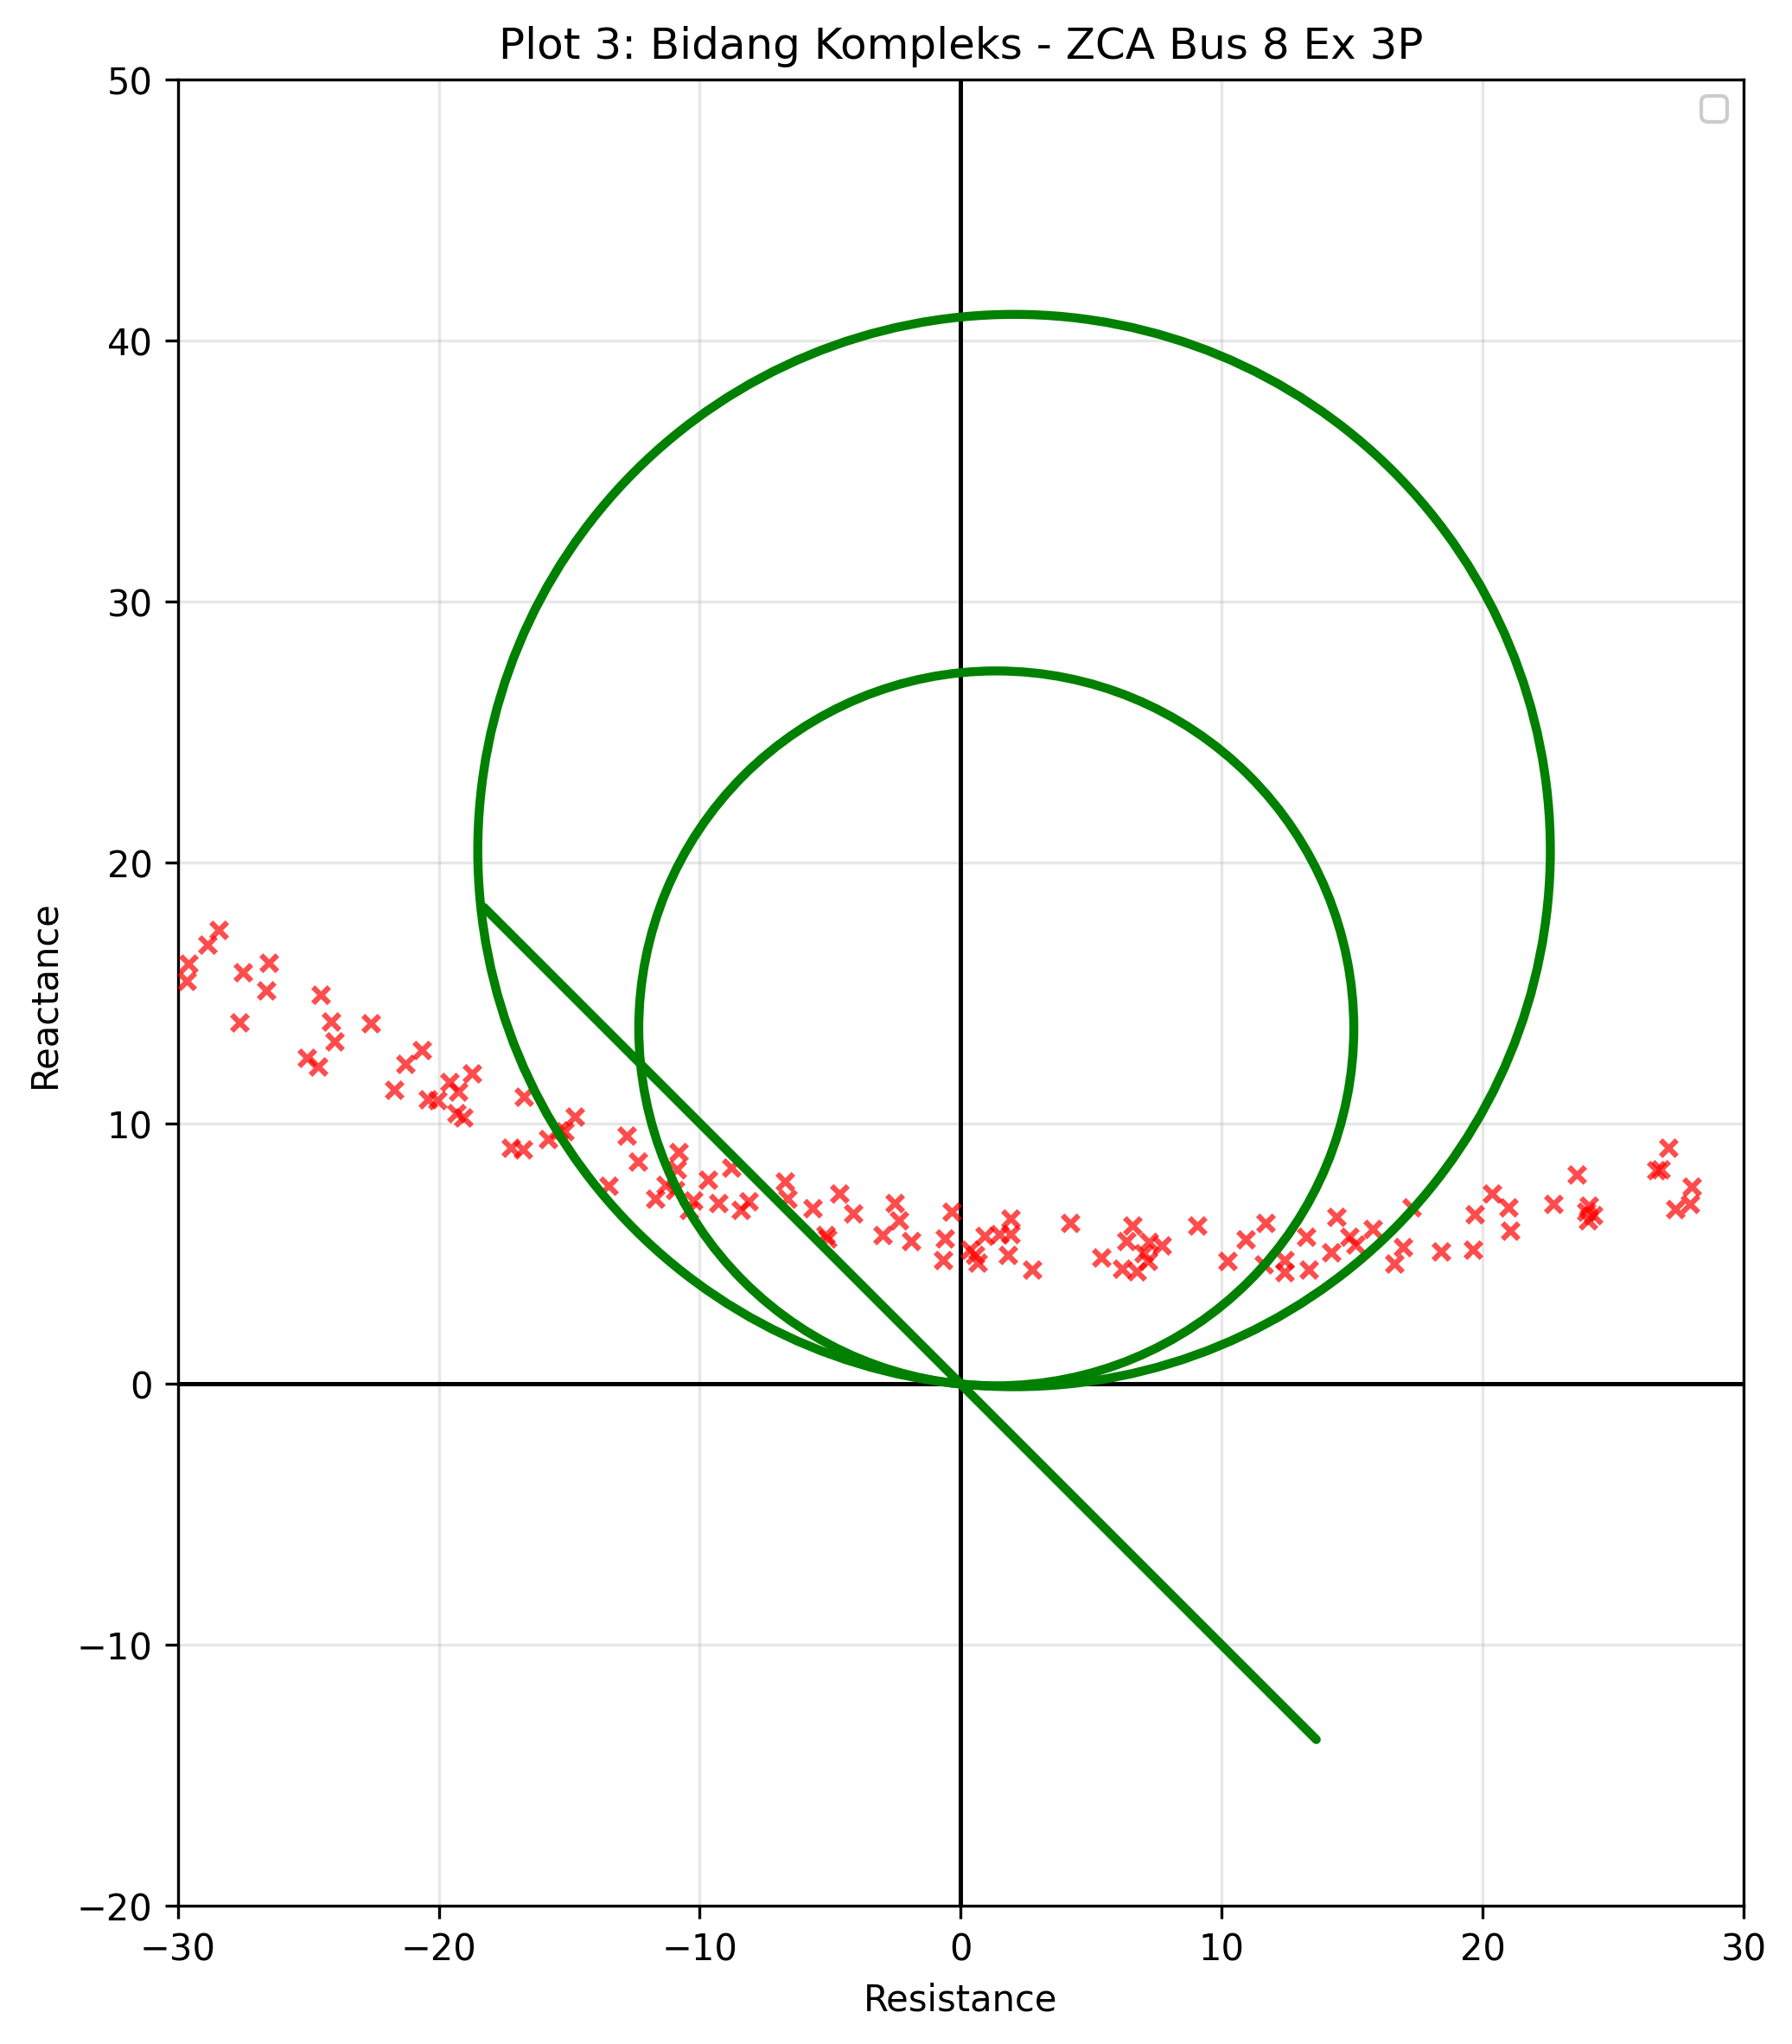
\includegraphics[width=0.8\textwidth]{contents/chapter-4/TIBR_03_ZCA_Bus_8_Ex_3P.png}
    \caption{Impedansi Tampak ZCA Bus 8 External 3P Fault}
    \label{fig:TIBR_03_ZCA_Bus_8_Ex_3P}
\end{figure}

Gambar \ref{fig:TIBR_03_ZCA_Bus_8_Ex_3P} menunjukkan impedansi tampak elemen fasa C ke fasa A pada relay 21 sisi Bus 8 saat terjadi gangguan eksternal tiga fasa. Hasil plot menunjukkan pola yang sama, yaitu titik impedansi tampak sempat mengalami \textit{overreach} terhadap zona 1. Relay tetap memberikan perintah trip karena arus telah mencapai batas maksimum untuk \textit{instant trip}, sebagaimana ditunjukkan oleh arus sekunder CT pada Gambar \ref{fig:Bus_8_Ex_3P}.

\begin{figure}[H]
    \centering
    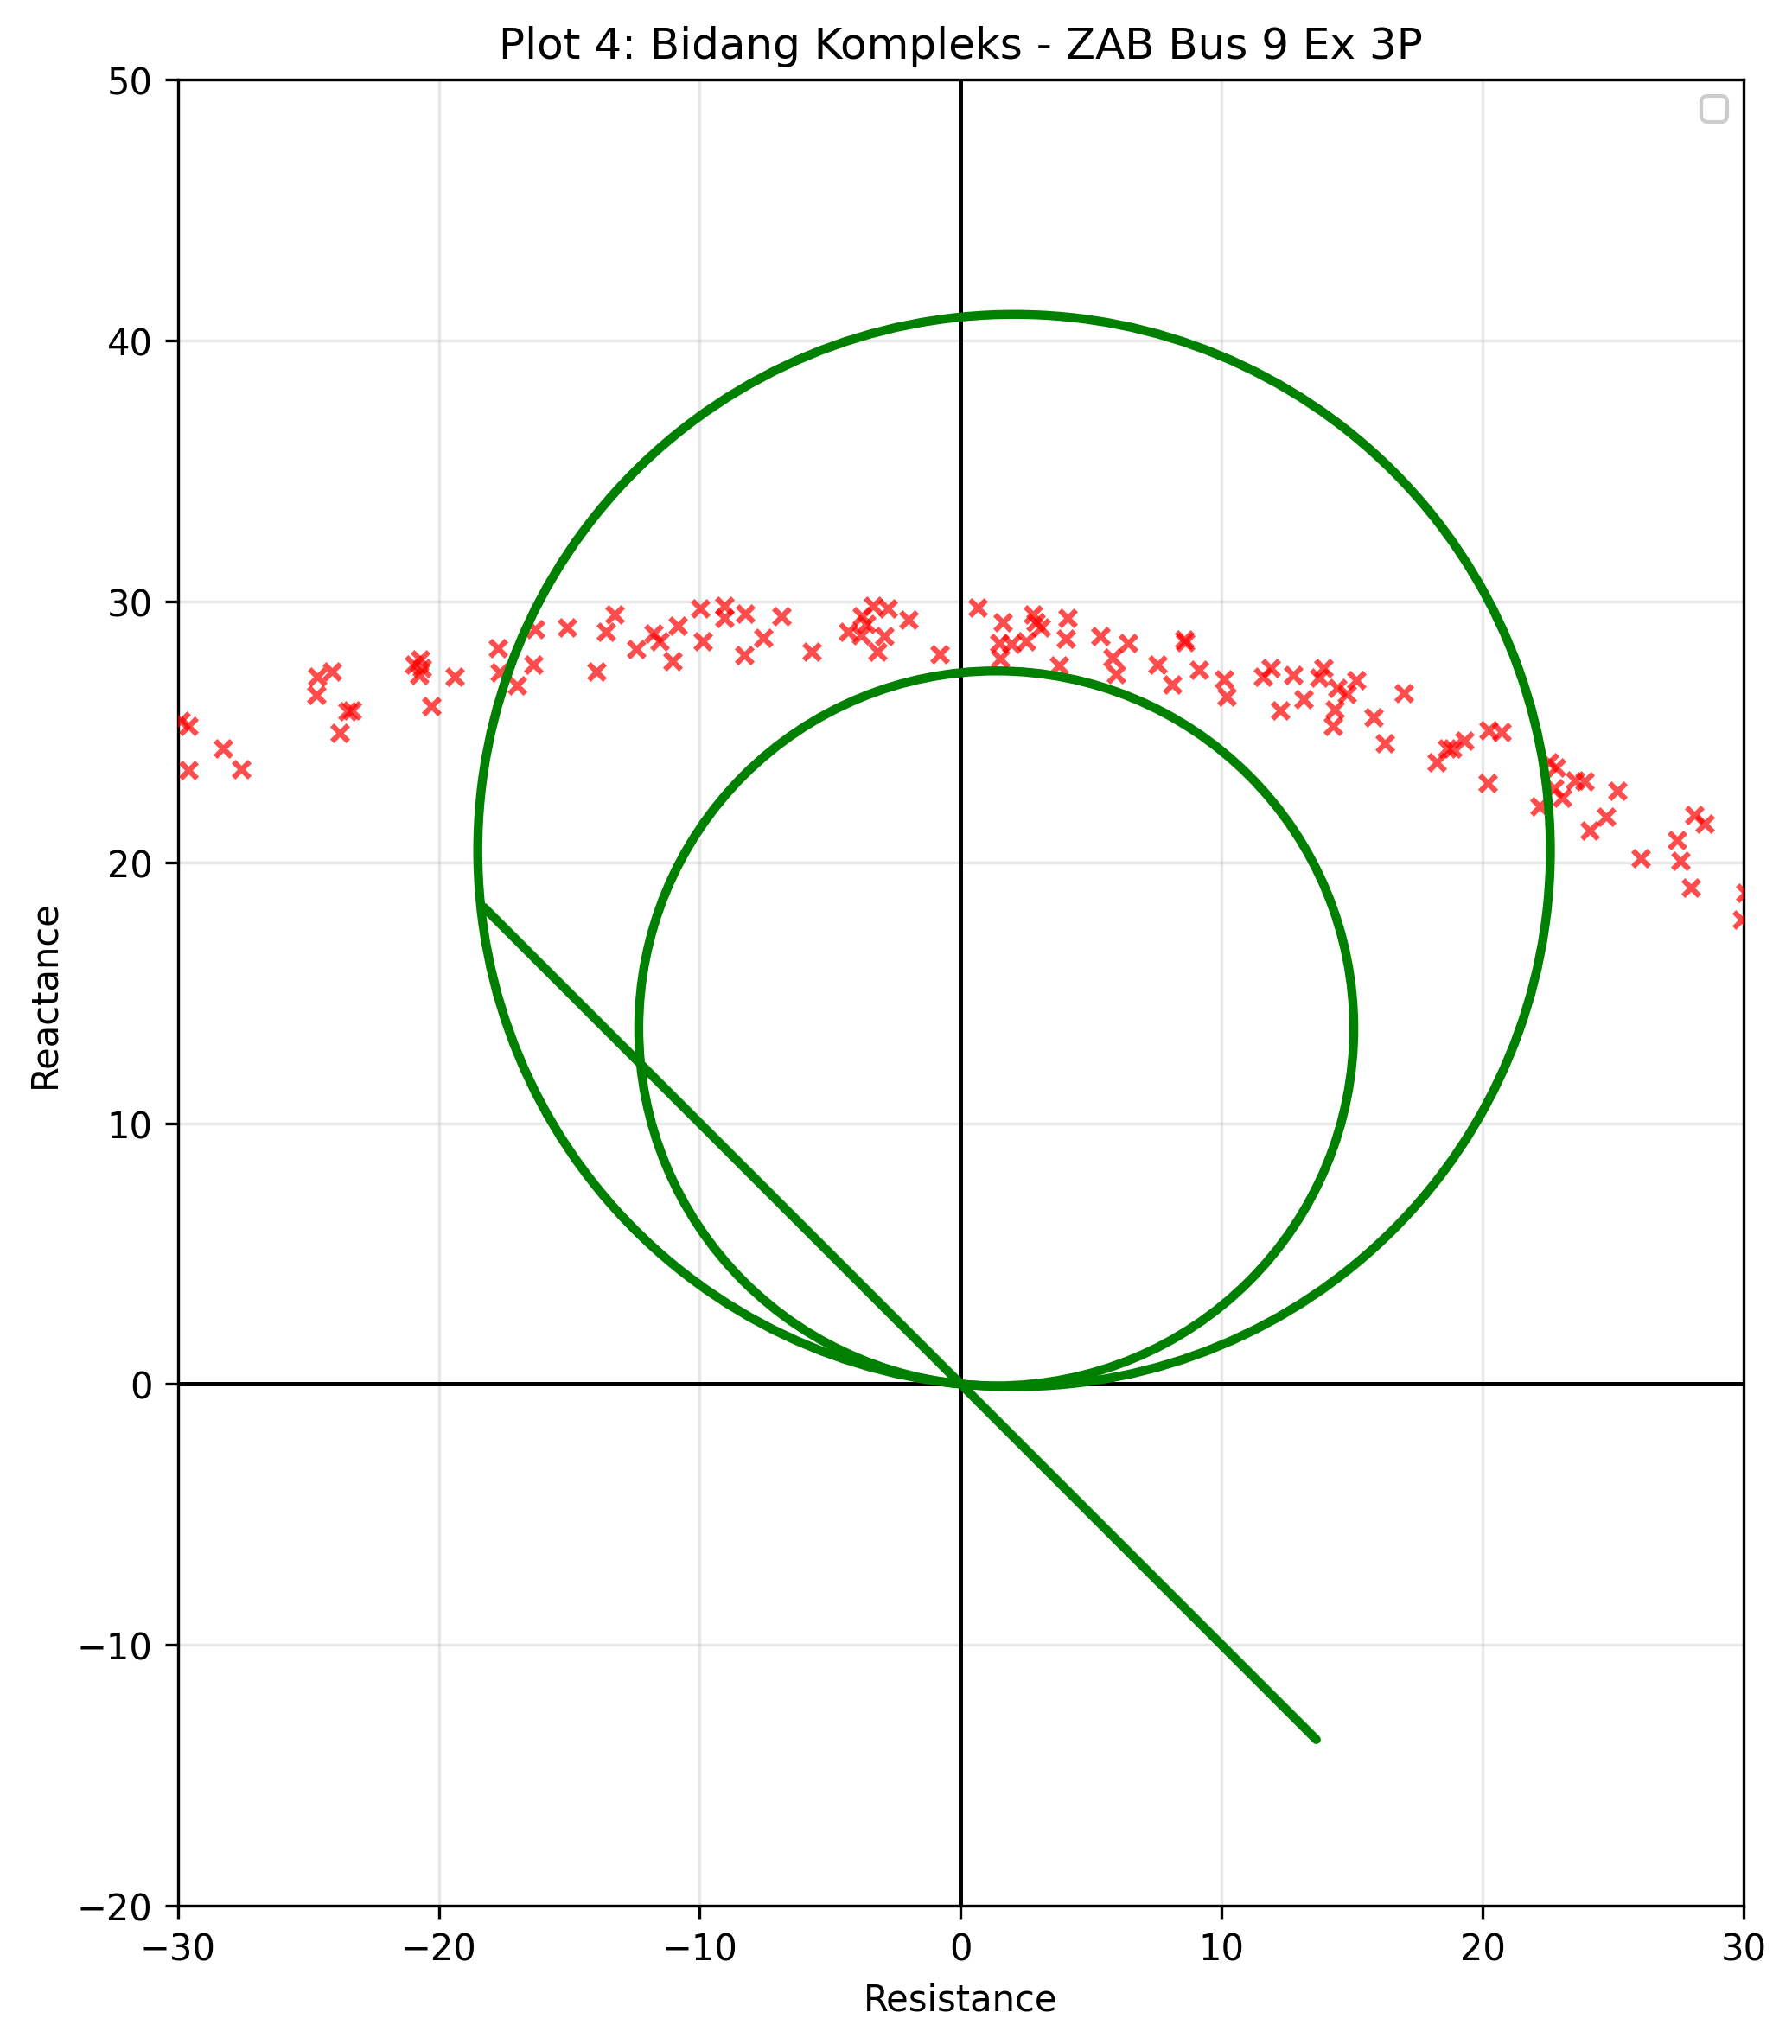
\includegraphics[width=0.8\textwidth]{contents/chapter-4/TIBR_04_ZAB_Bus_9_Ex_3P.png}
    \caption{Impedansi Tampak ZAB Bus 9 External 3P Fault}
    \label{fig:TIBR_04_ZAB_Bus_9_Ex_3P}
\end{figure}

Gambar \ref{fig:TIBR_04_ZAB_Bus_9_Ex_3P} menunjukkan impedansi tampak elemen fasa A ke fasa B yang dibaca oleh relay 21 melalui CT dan VT pada Bus 9. Pada gangguan eksternal tiga fasa, relay 21 sisi Bus 9 tidak membaca gangguan sebagai gangguan yang berada di arah depan relay. Oleh karena itu, relay tidak mengirimkan sinyal trip kepada CB, sehingga respons pada sisi Bus 9 masih sesuai untuk gangguan eksternal.

\begin{figure}[H]
    \centering
    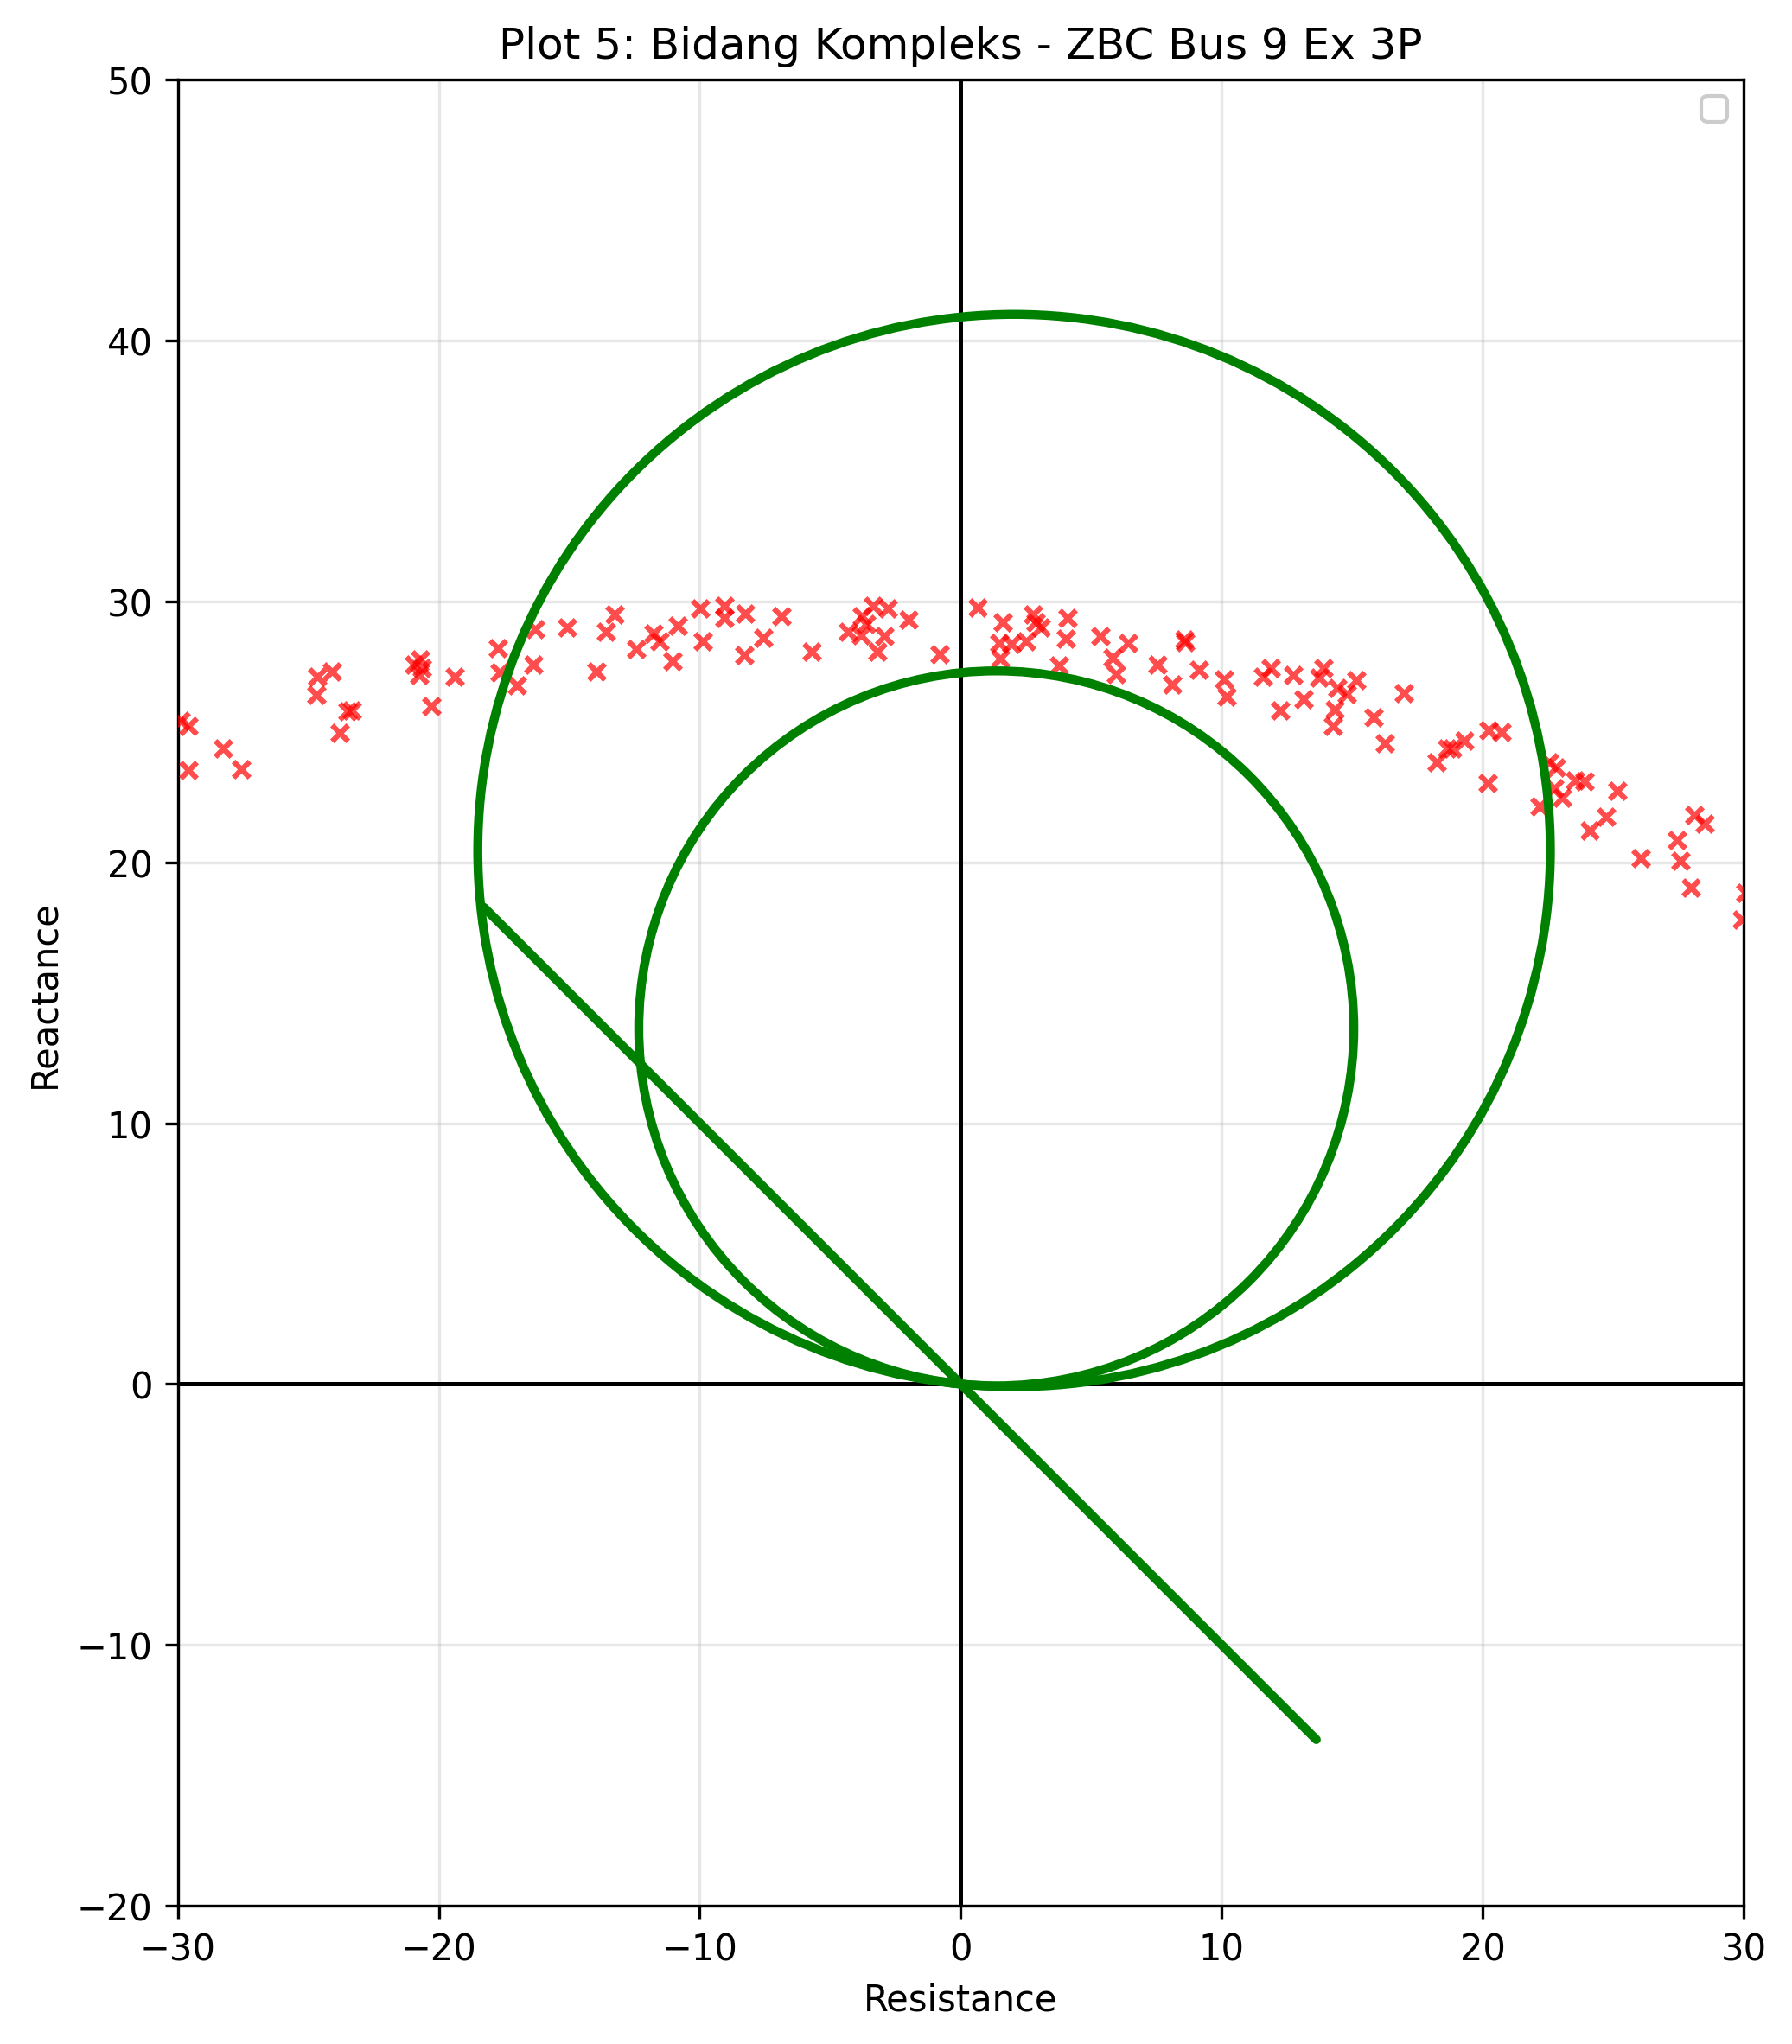
\includegraphics[width=0.8\textwidth]{contents/chapter-4/TIBR_05_ZBC_Bus_9_Ex_3P.png}
    \caption{Impedansi Tampak ZBC Bus 9 External 3P Fault}
    \label{fig:TIBR_05_ZBC_Bus_9_Ex_3P}
\end{figure}

Gambar \ref{fig:TIBR_05_ZBC_Bus_9_Ex_3P} menunjukkan impedansi tampak elemen fasa B ke fasa C yang dibaca oleh relay 21 melalui CT dan VT pada Bus 9. Hasil plot menunjukkan bahwa relay tidak mendeteksi gangguan eksternal tiga fasa sebagai gangguan di depan relay. Dengan pembacaan tersebut, relay 21 sisi Bus 9 tidak mengirimkan sinyal trip kepada CB dan tetap berada pada kondisi yang diharapkan untuk gangguan eksternal.

\begin{figure}[H]
    \centering
    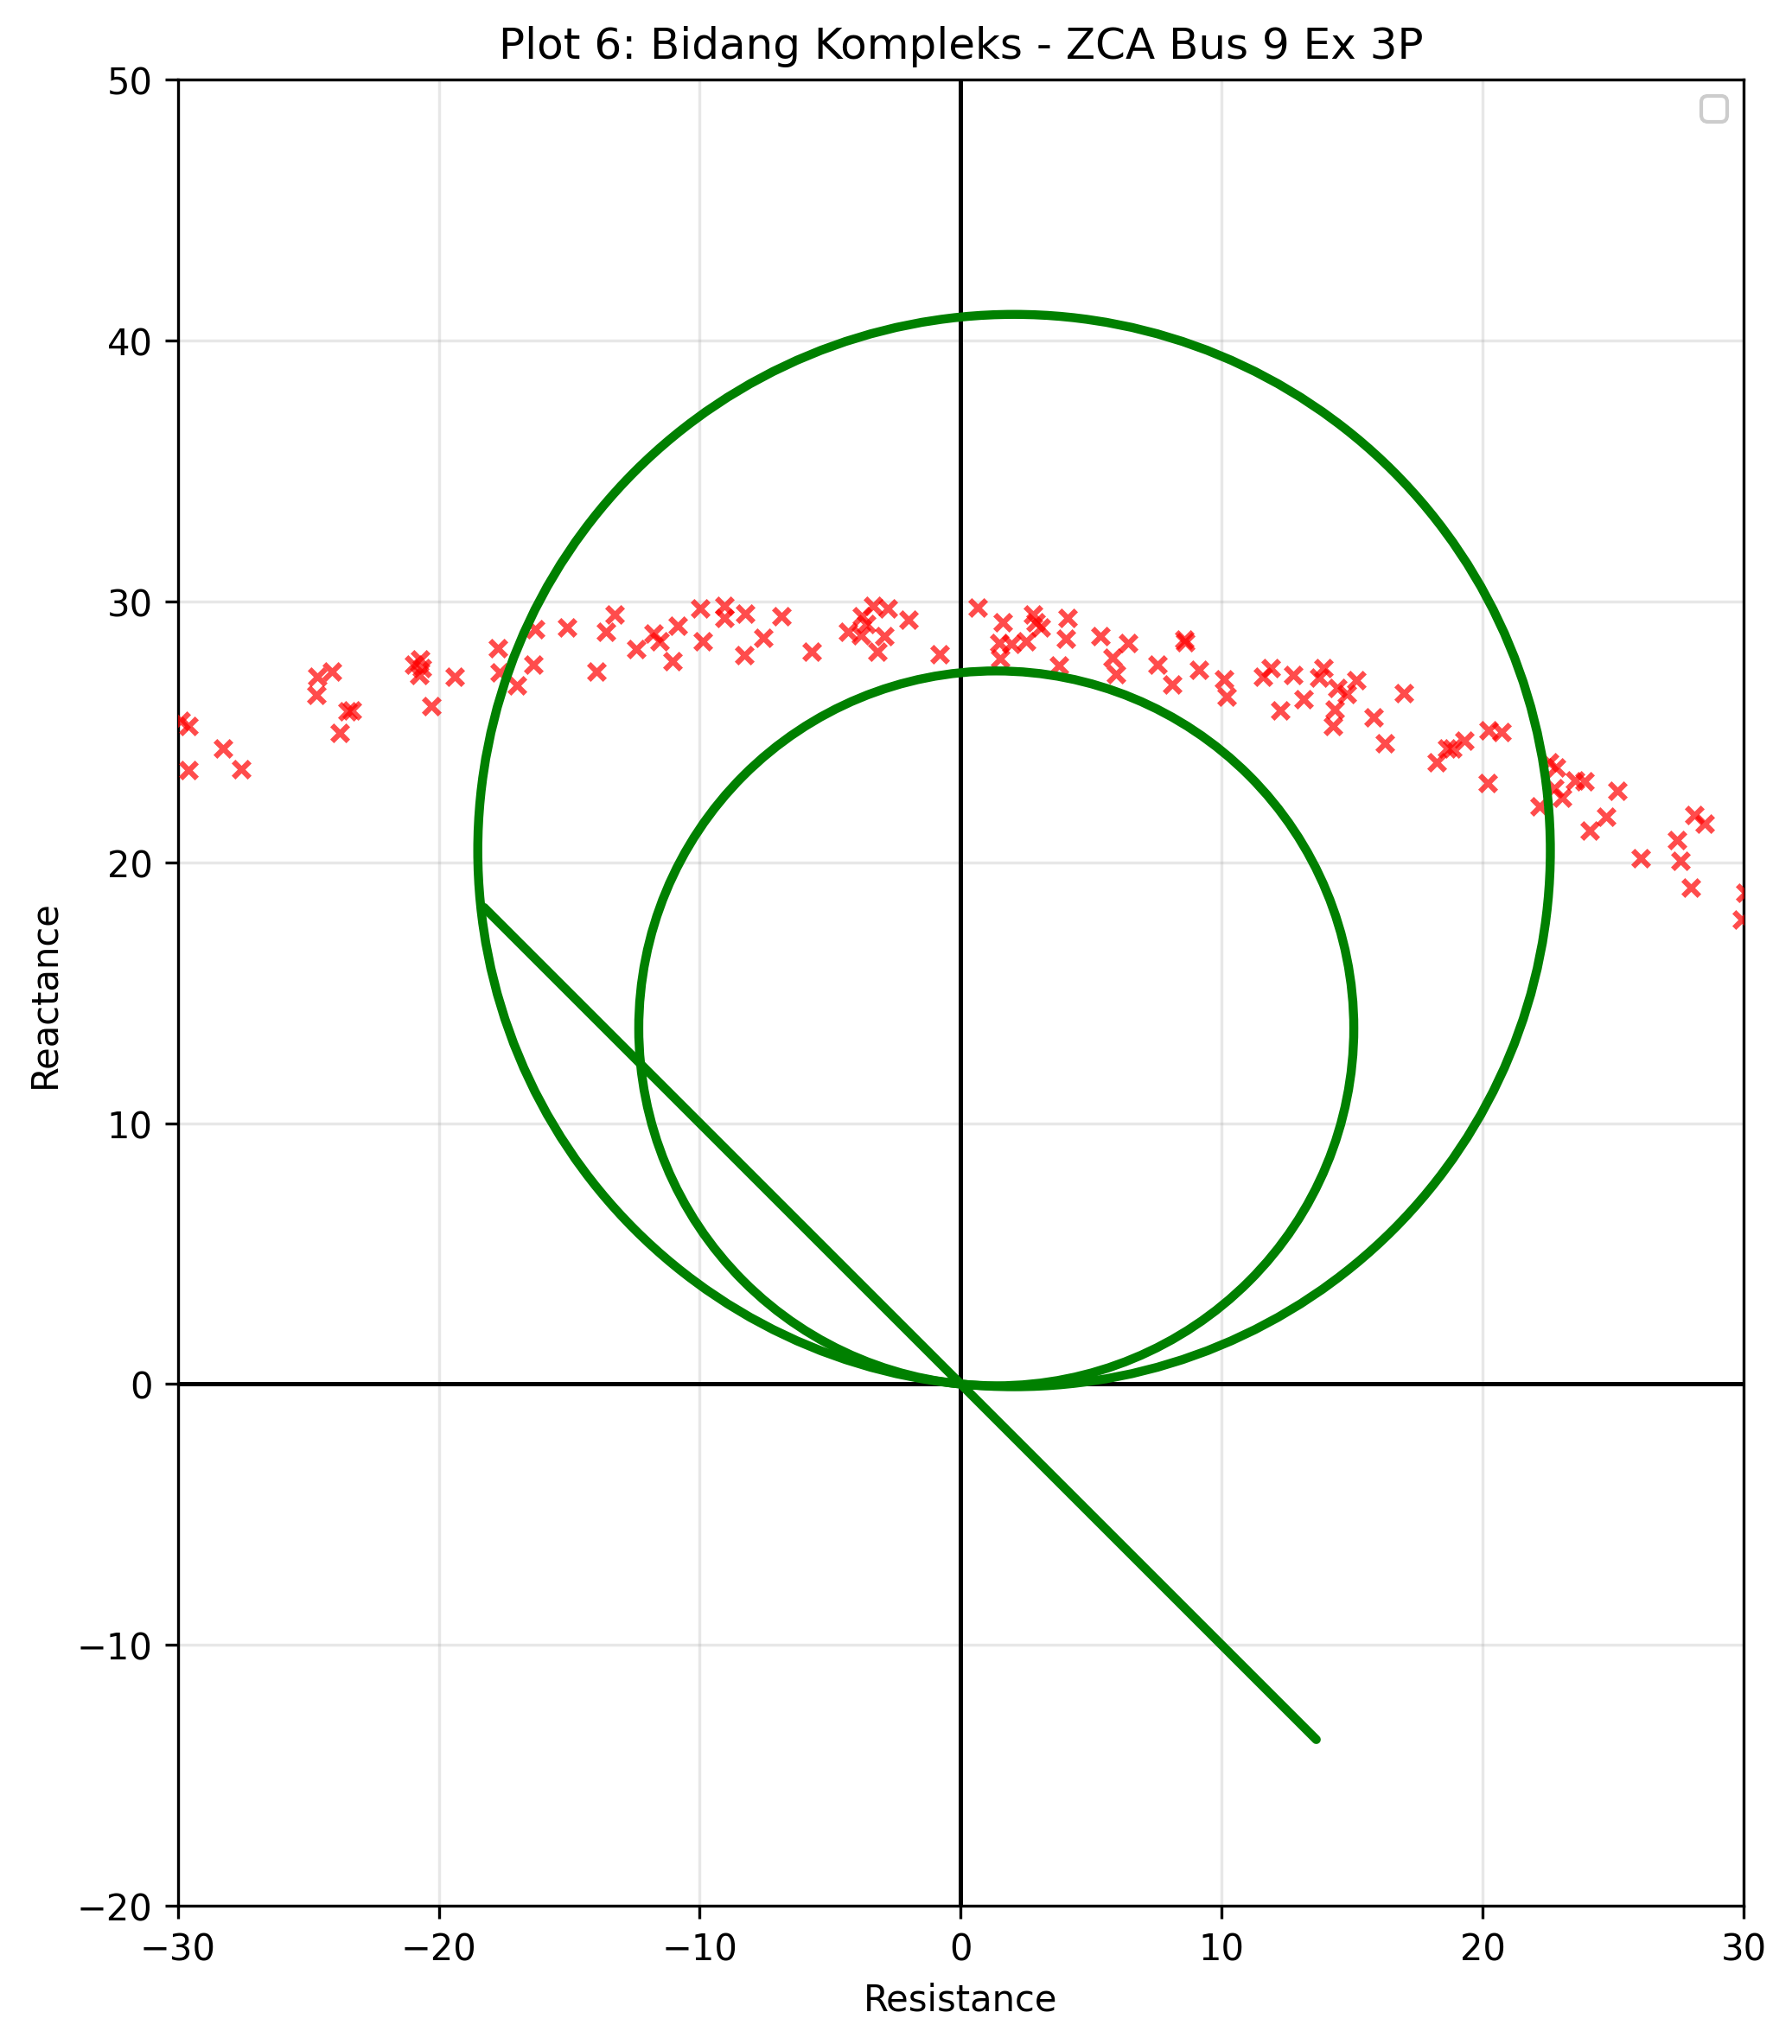
\includegraphics[width=0.8\textwidth]{contents/chapter-4/TIBR_06_ZCA_Bus_9_Ex_3P.png}
    \caption{Impedansi Tampak ZCA Bus 9 External 3P Fault}
    \label{fig:TIBR_06_ZCA_Bus_9_Ex_3P}
\end{figure}

Gambar \ref{fig:TIBR_06_ZCA_Bus_9_Ex_3P} menunjukkan impedansi tampak elemen fasa C ke fasa A yang dibaca oleh relay 21 melalui CT dan VT pada Bus 9. Pada kondisi gangguan eksternal tiga fasa, relay tidak membaca gangguan berada pada arah depan relay. Akibatnya, relay 21 sisi Bus 9 tidak mengirimkan sinyal trip kepada CB, sehingga responsnya konsisten dengan dua elemen fasa-fasa sebelumnya.

\begin{figure}[H]
    \centering
    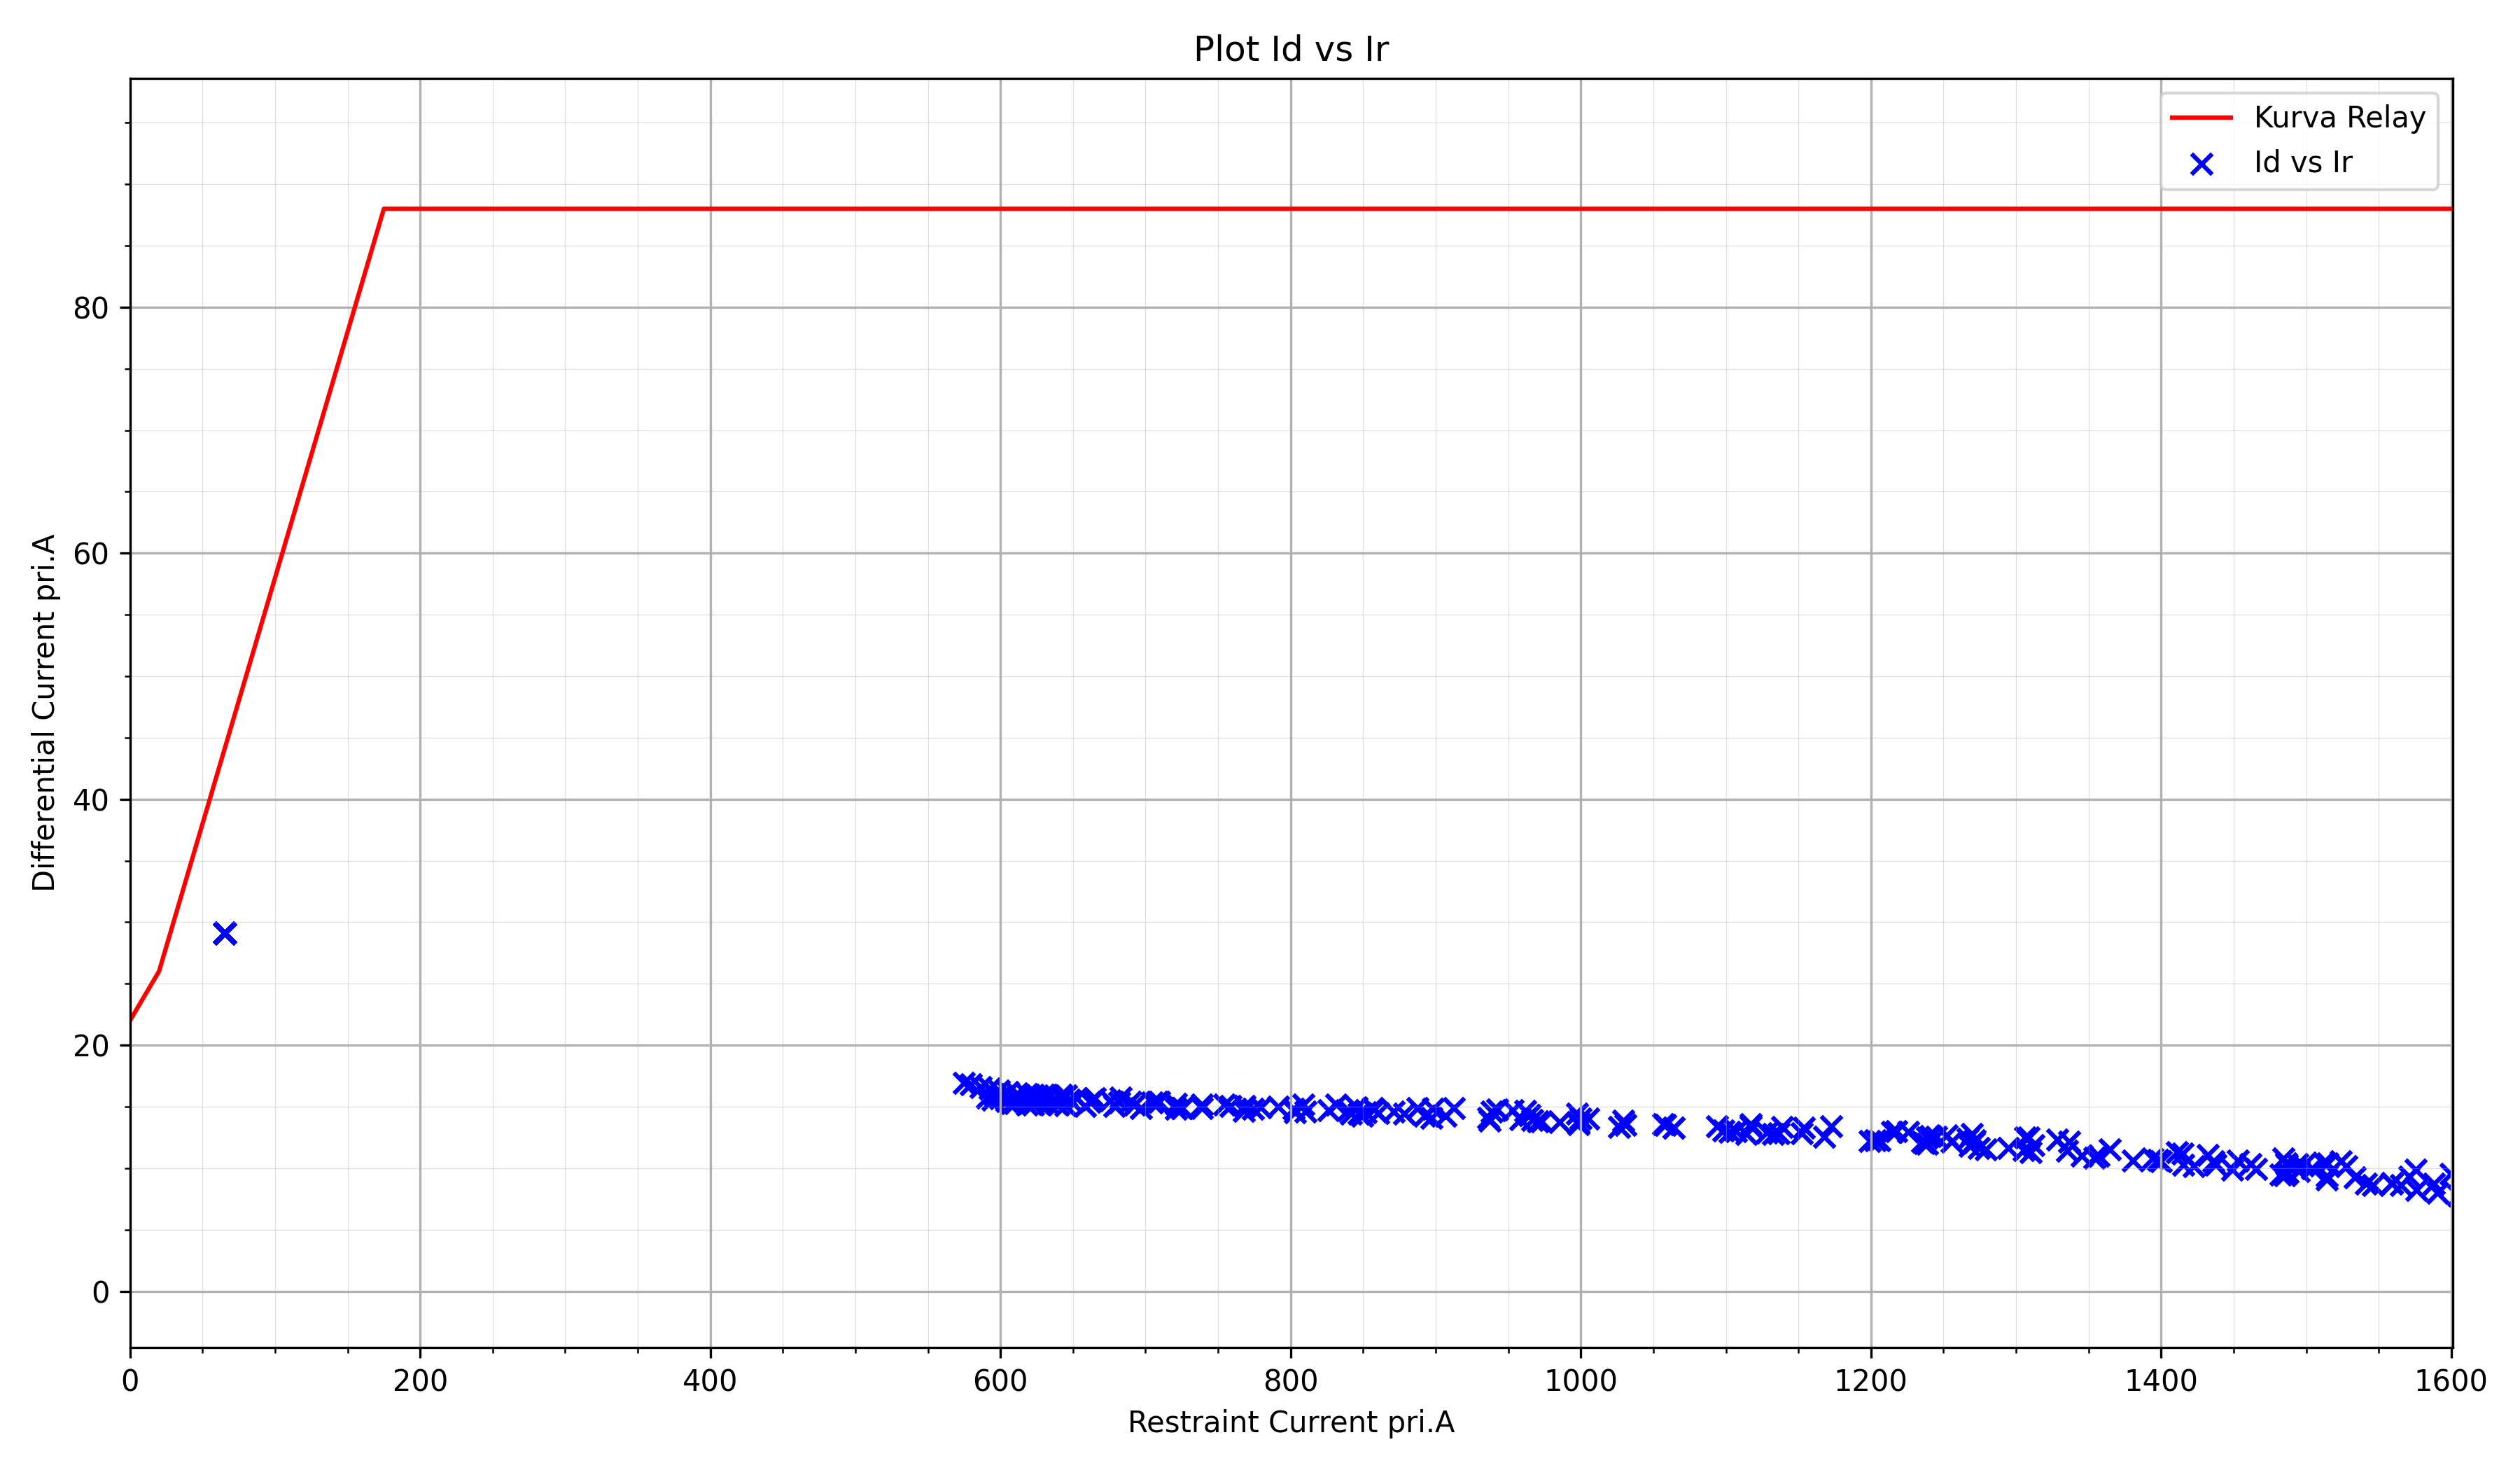
\includegraphics[width=0.8\textwidth]{contents/chapter-4/87LTIBR_plot_Ax1_Ay1.png}
    \caption{Current Comparison Differential Fasa A External 3P Fault}
    \label{fig:87LTIBR_plot_Ax1_Ay1}
\end{figure}

Gambar \ref{fig:87LTIBR_plot_Ax1_Ay1} menunjukkan plot \textit{current comparison differential} pada fasa A saat terjadi gangguan eksternal tiga fasa. Titik arus berada di bawah batas operasi yang ditentukan oleh setting relay. Kondisi ini menunjukkan bahwa relay 87L tidak membaca gangguan sebagai gangguan internal dan tidak memerintahkan trip pada CB.

\begin{figure}[H]
    \centering
    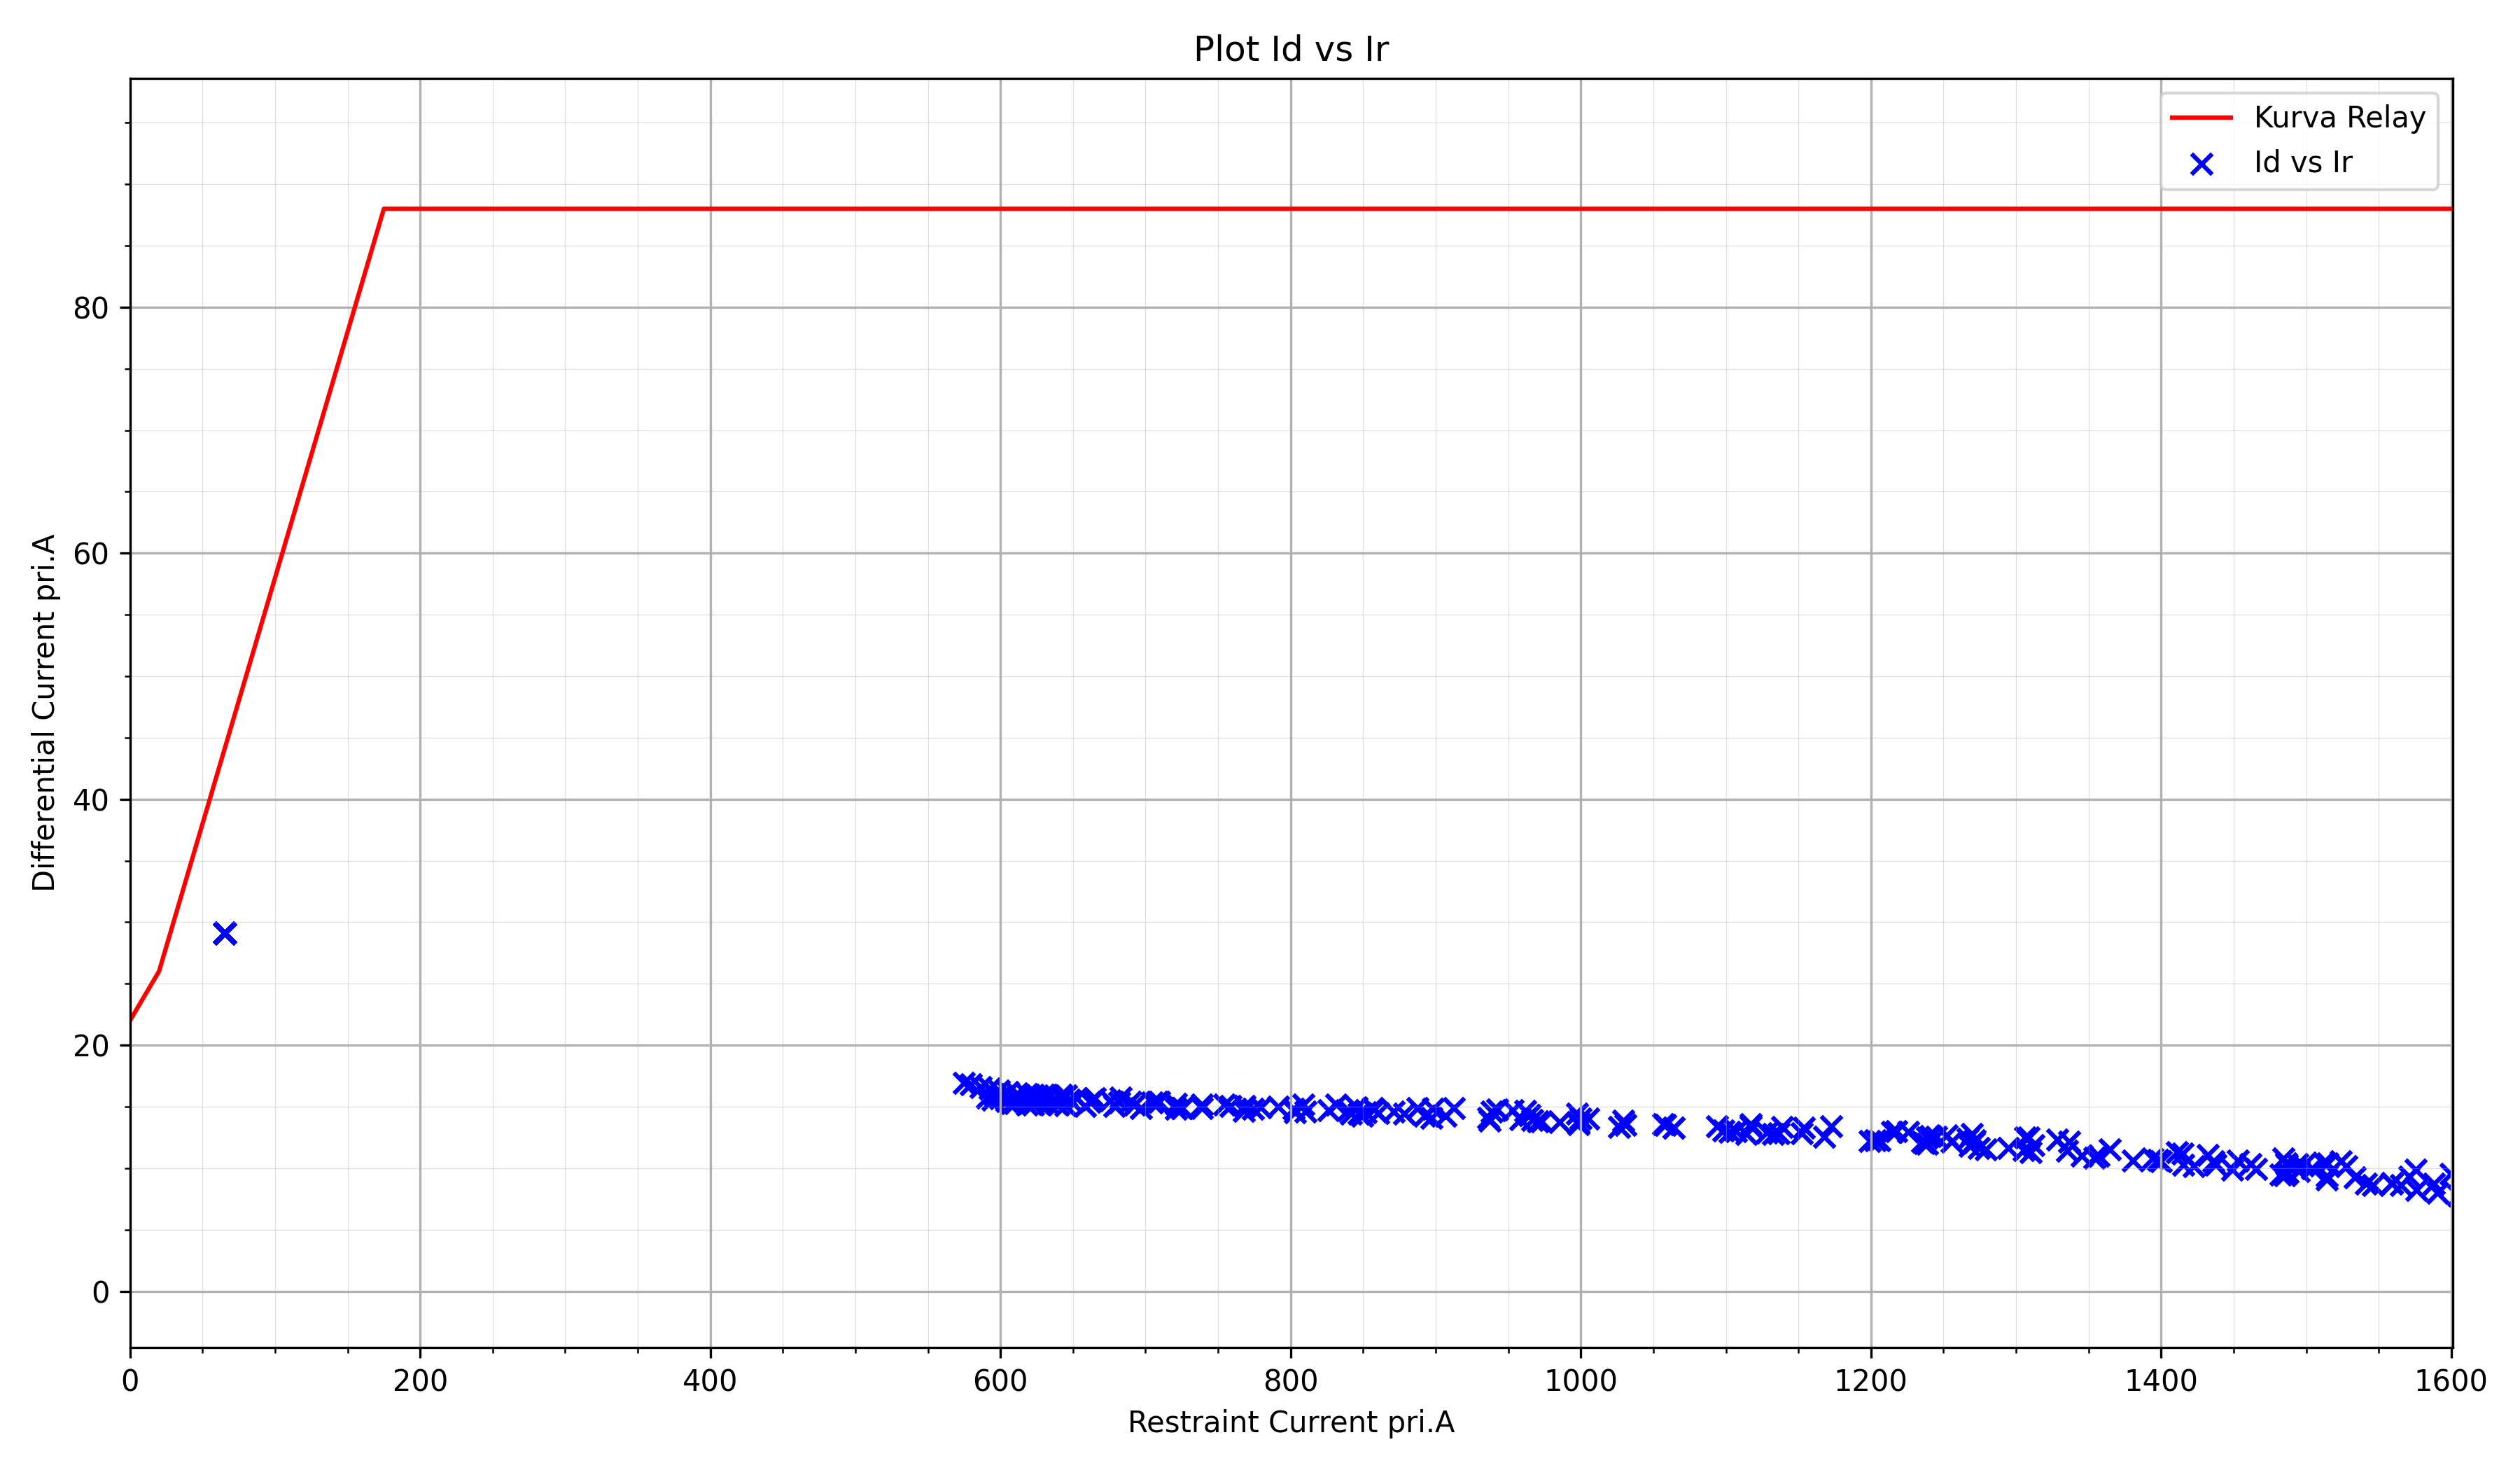
\includegraphics[width=0.8\textwidth]{contents/chapter-4/87LTIBR_plot_Bx1_By1.png}
    \caption{Current Comparison Differential Fasa B External 3P Fault}
    \label{fig:87LTIBR_plot_Bx1_By1}
\end{figure}

Gambar \ref{fig:87LTIBR_plot_Bx1_By1} menunjukkan plot \textit{current comparison differential} pada fasa B saat terjadi gangguan eksternal tiga fasa. Titik arus pada fasa B juga berada di bawah batas operasi yang ditentukan oleh setting relay. Dengan demikian, relay 87L tetap berada pada daerah penahan dan tidak mengeluarkan perintah trip kepada CB.

\begin{figure}[H]
    \centering
    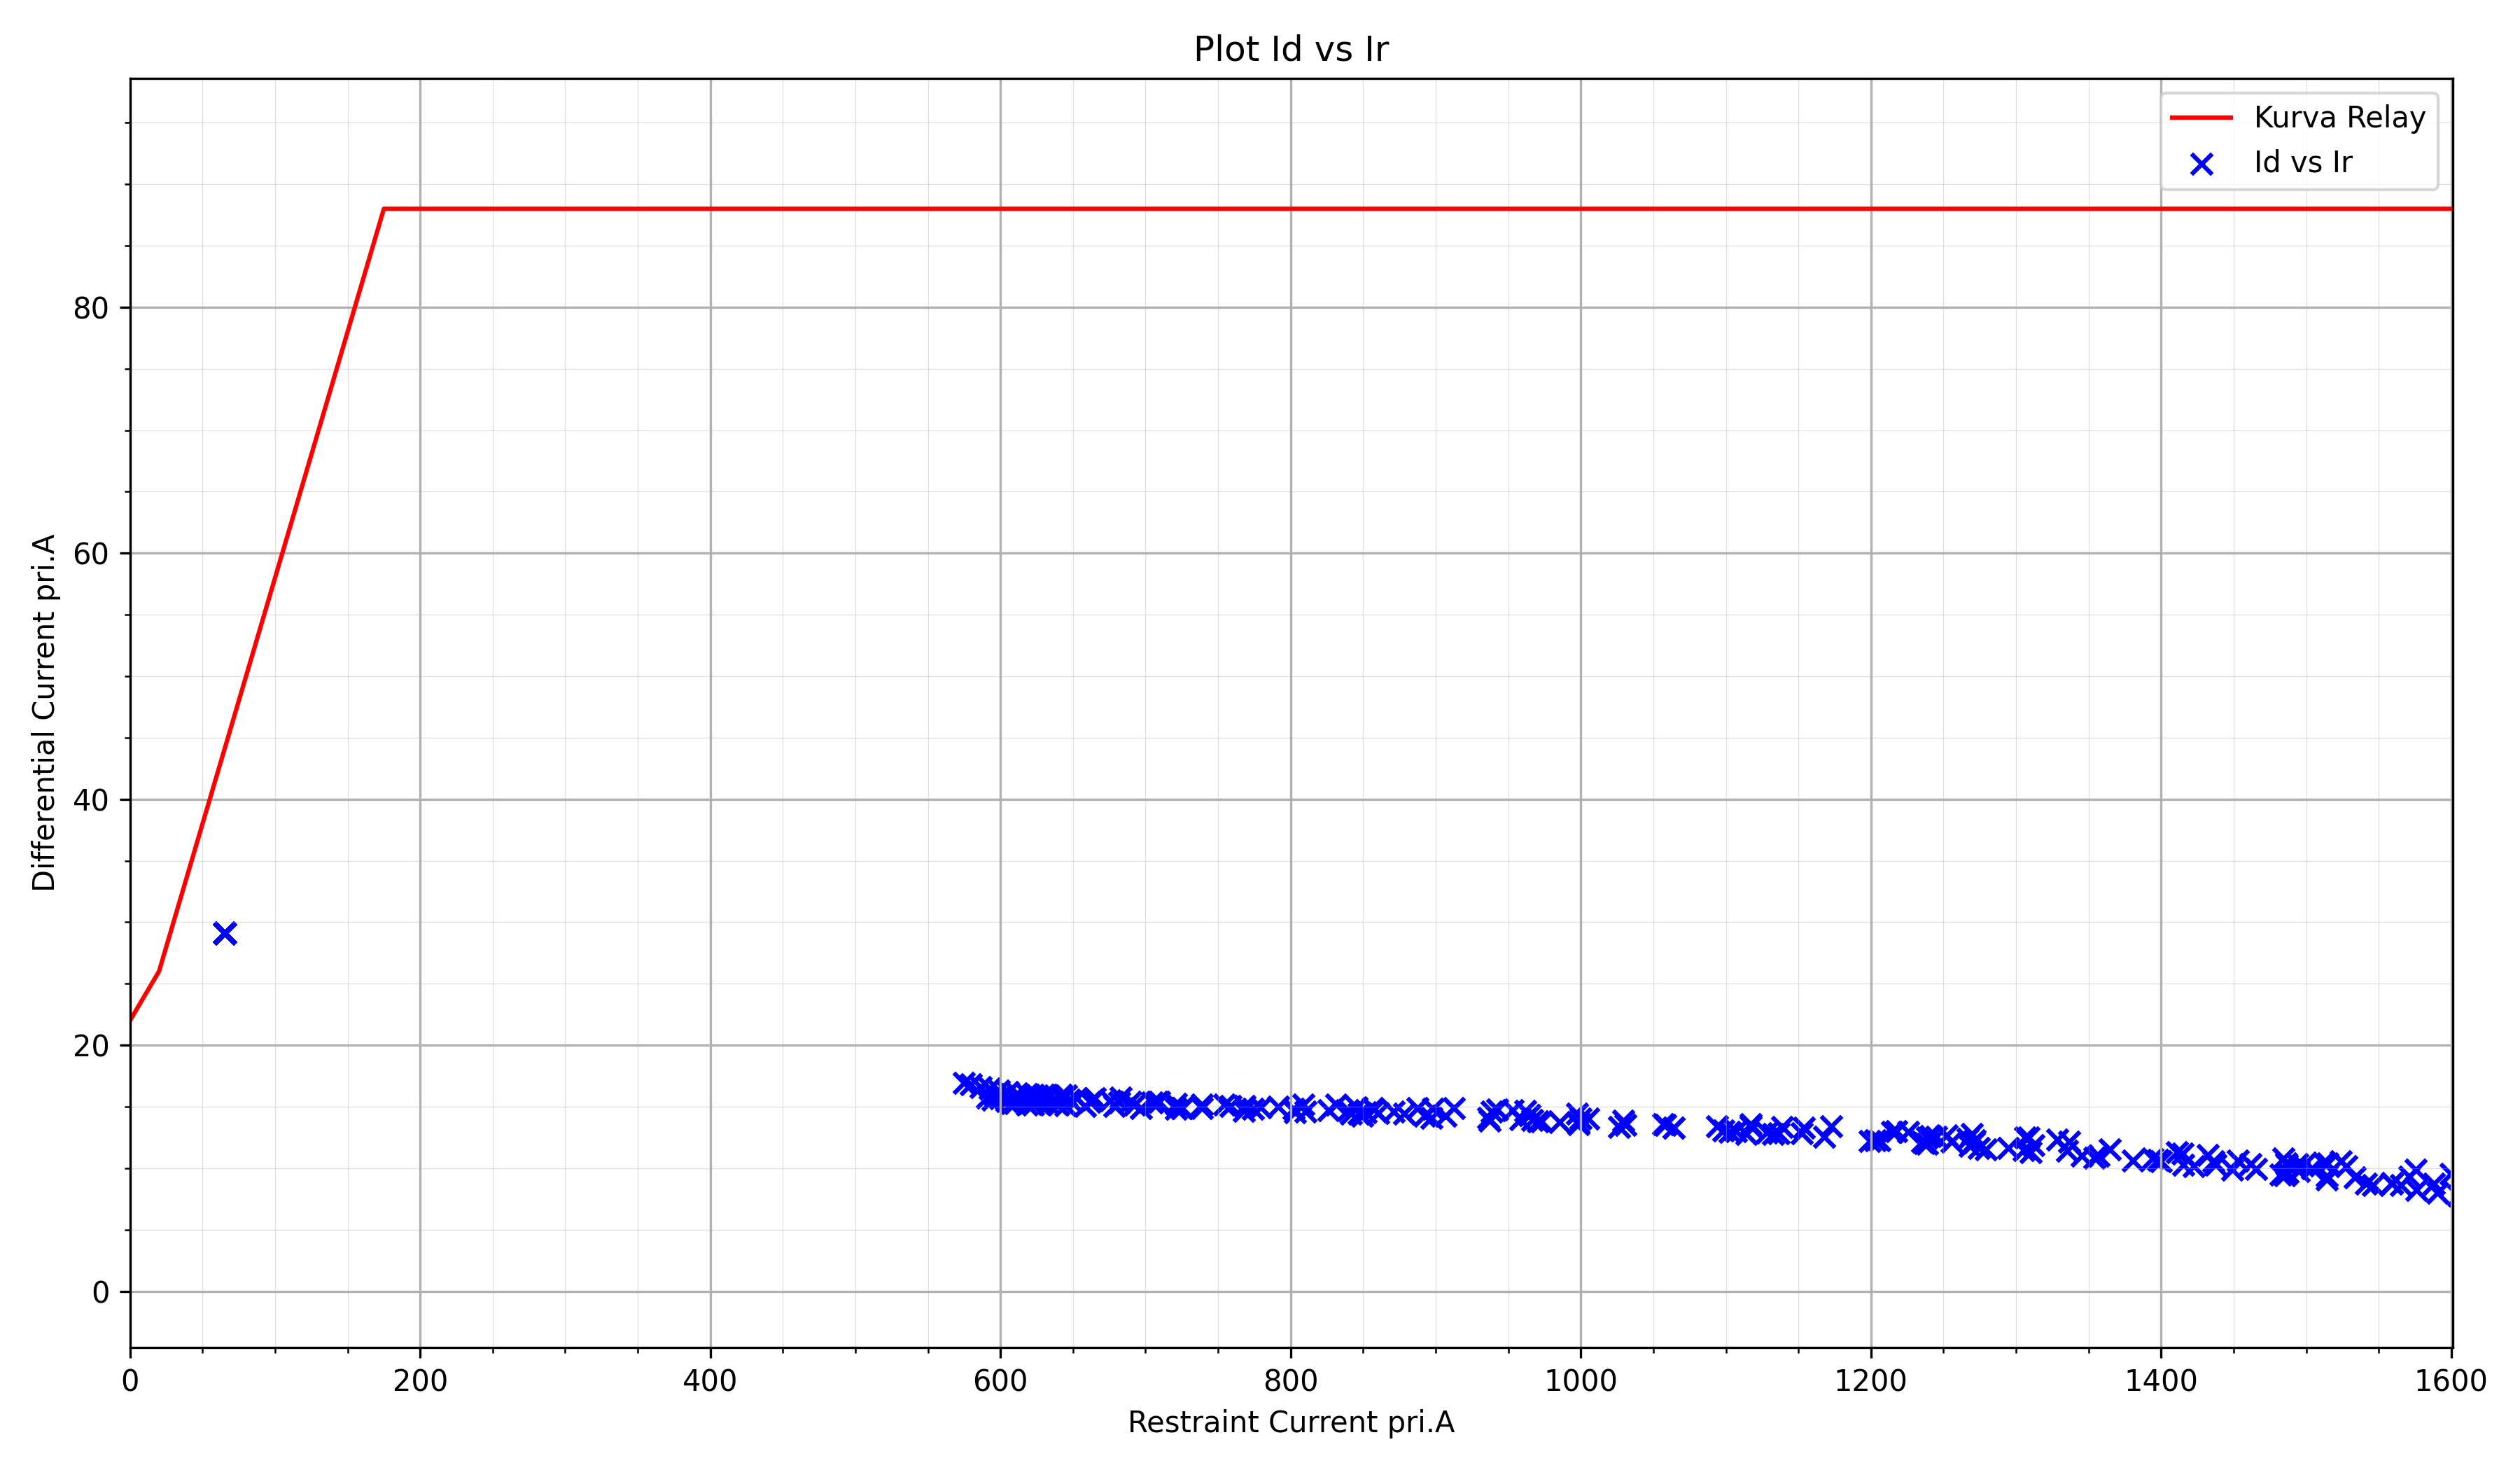
\includegraphics[width=0.8\textwidth]{contents/chapter-4/87LTIBR_plot_Cx1_Cy1.png}
    \caption{Current Comparison Differential Fasa C External 3P Fault}
    \label{fig:87LTIBR_plot_Cx1_Cy1}
\end{figure}

Gambar \ref{fig:87LTIBR_plot_Cx1_Cy1} menunjukkan plot \textit{current comparison differential} pada fasa C saat terjadi gangguan eksternal tiga fasa. Titik arus berada di bawah batas operasi relay, sehingga relay 87L membaca kondisi tersebut sebagai gangguan di luar daerah proteksinya. Oleh karena itu, relay tidak memberikan perintah trip kepada CB.

\subsection{Respons Relay terhadap gangguan External Single Line to Ground (SLG)}
\label{subsec:tanpa_IBR_ex_slg}

\begin{figure}[H]
    \centering
    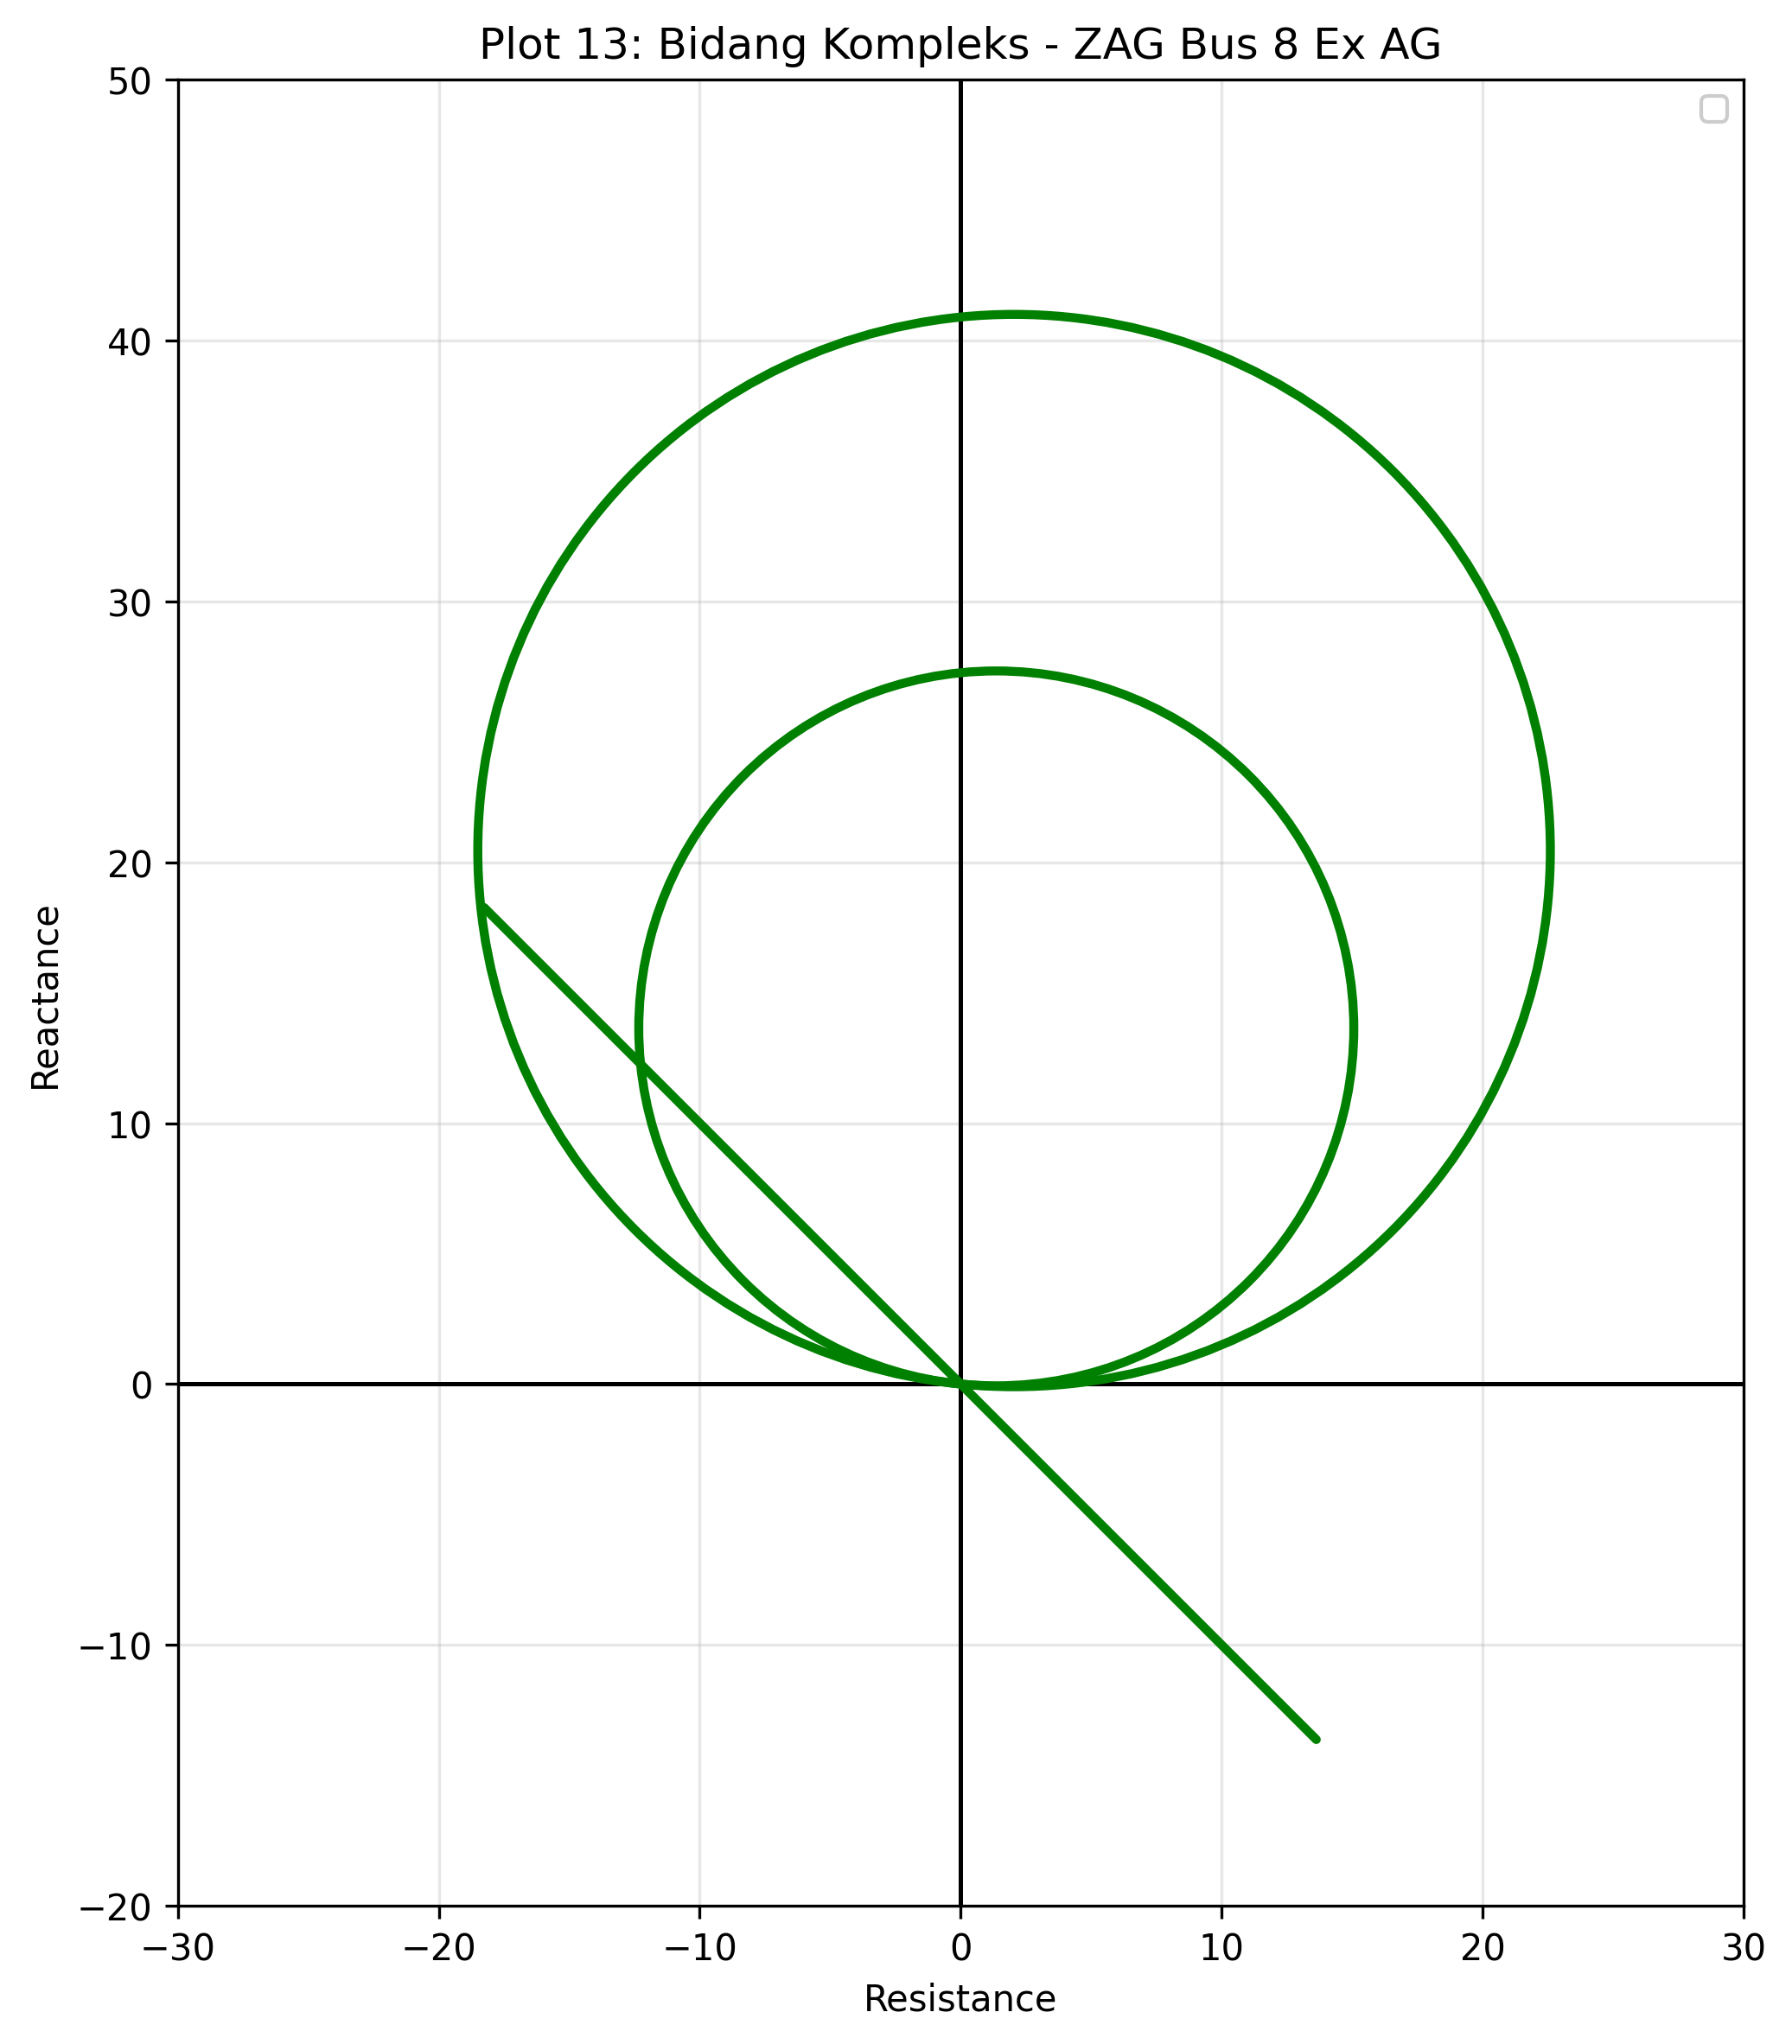
\includegraphics[width=0.8\textwidth]{contents/chapter-4/TIBR_13_ZAG_Bus_8_Ex_AG.png}
    \caption{Impedansi Tampak ZAG Bus 8 External SLG Fault}
    \label{fig:TIBR_13_ZAG_Bus_8_Ex_AG}
\end{figure}

\begin{figure}[H]
    \centering
    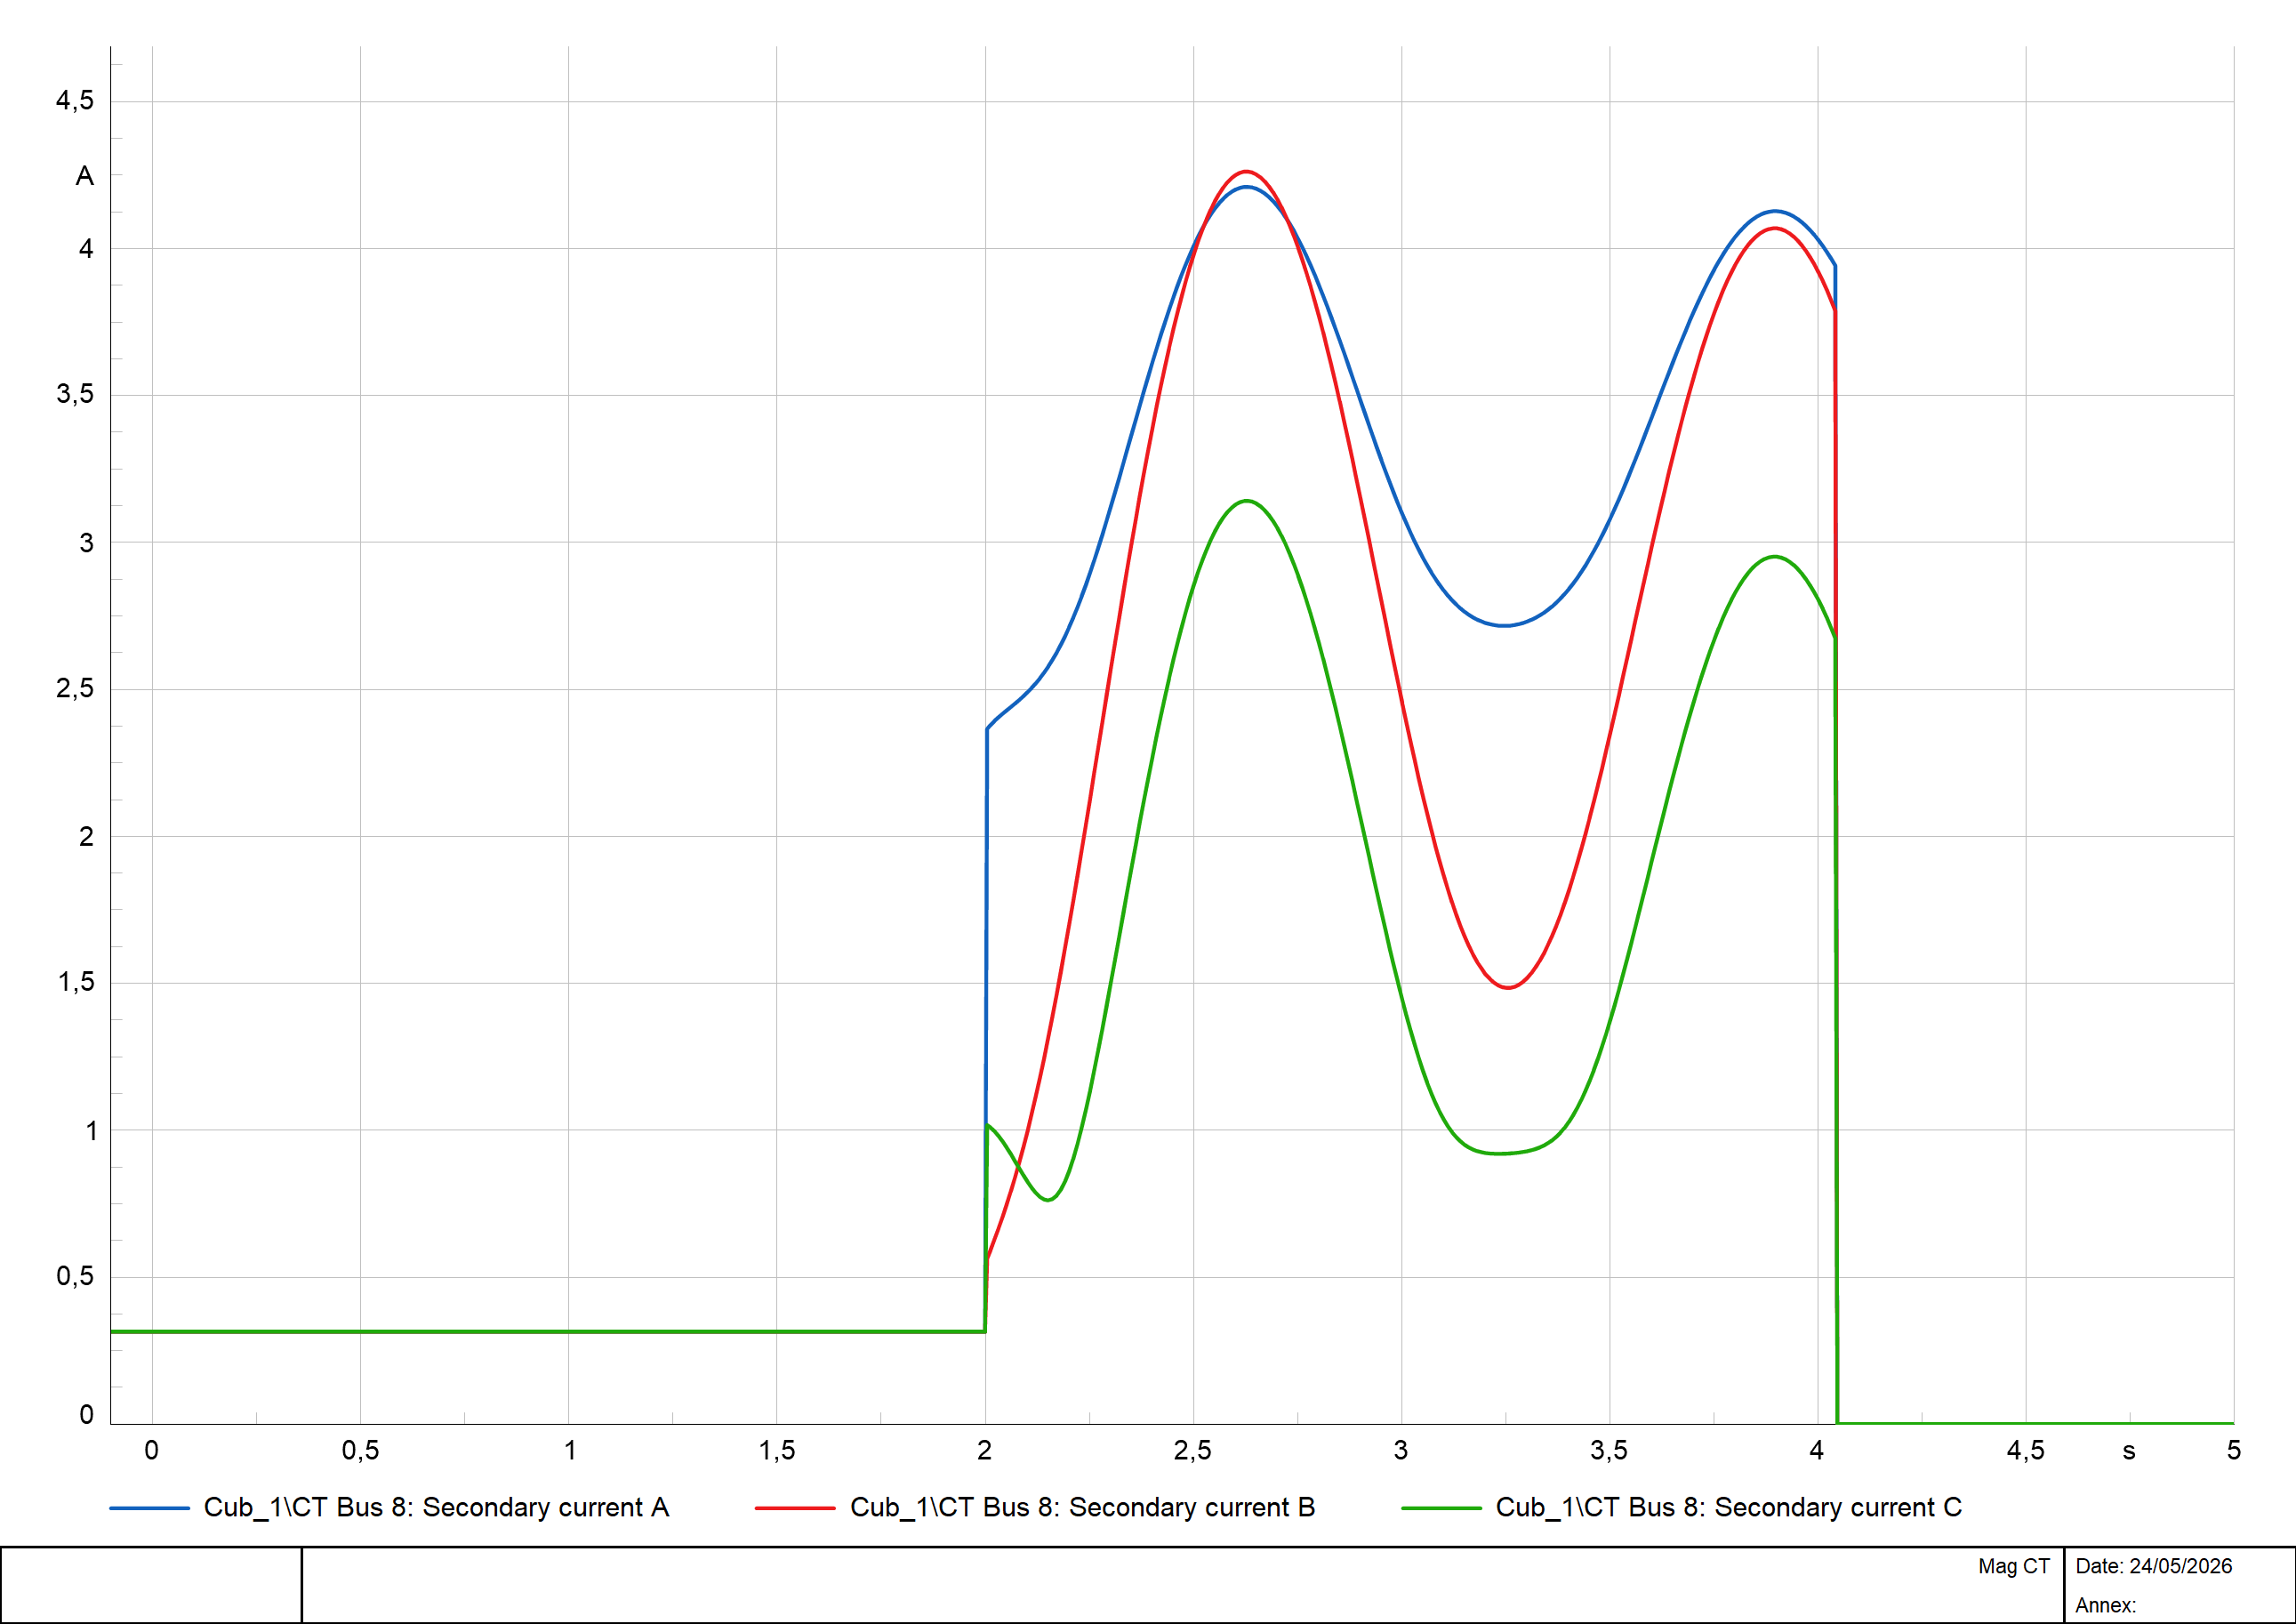
\includegraphics[width=0.8\textwidth]{contents/chapter-4/Bus_8_Ex_SLG.png}
    \caption{Arus Sekunder CT Bus 8 Pada External SLG Fault}
    \label{fig:Bus_8_Ex_SLG}
\end{figure}

Gambar \ref{fig:TIBR_13_ZAG_Bus_8_Ex_AG} menunjukkan impedansi tampak loop fasa A dengan ground yang dibaca oleh relay 21 melalui CT dan VT pada Bus 8. Pada gangguan eksternal SLG, impedansi tampak yang terbaca tidak masuk ke dalam zona proteksi. Namun, relay tetap memberikan perintah trip melalui \textit{backup trip} karena arus yang mengalir sudah membuat relay aktif, sebagaimana ditunjukkan pada Gambar \ref{fig:Bus_8_Ex_SLG}.

\begin{figure}[H]
    \centering
    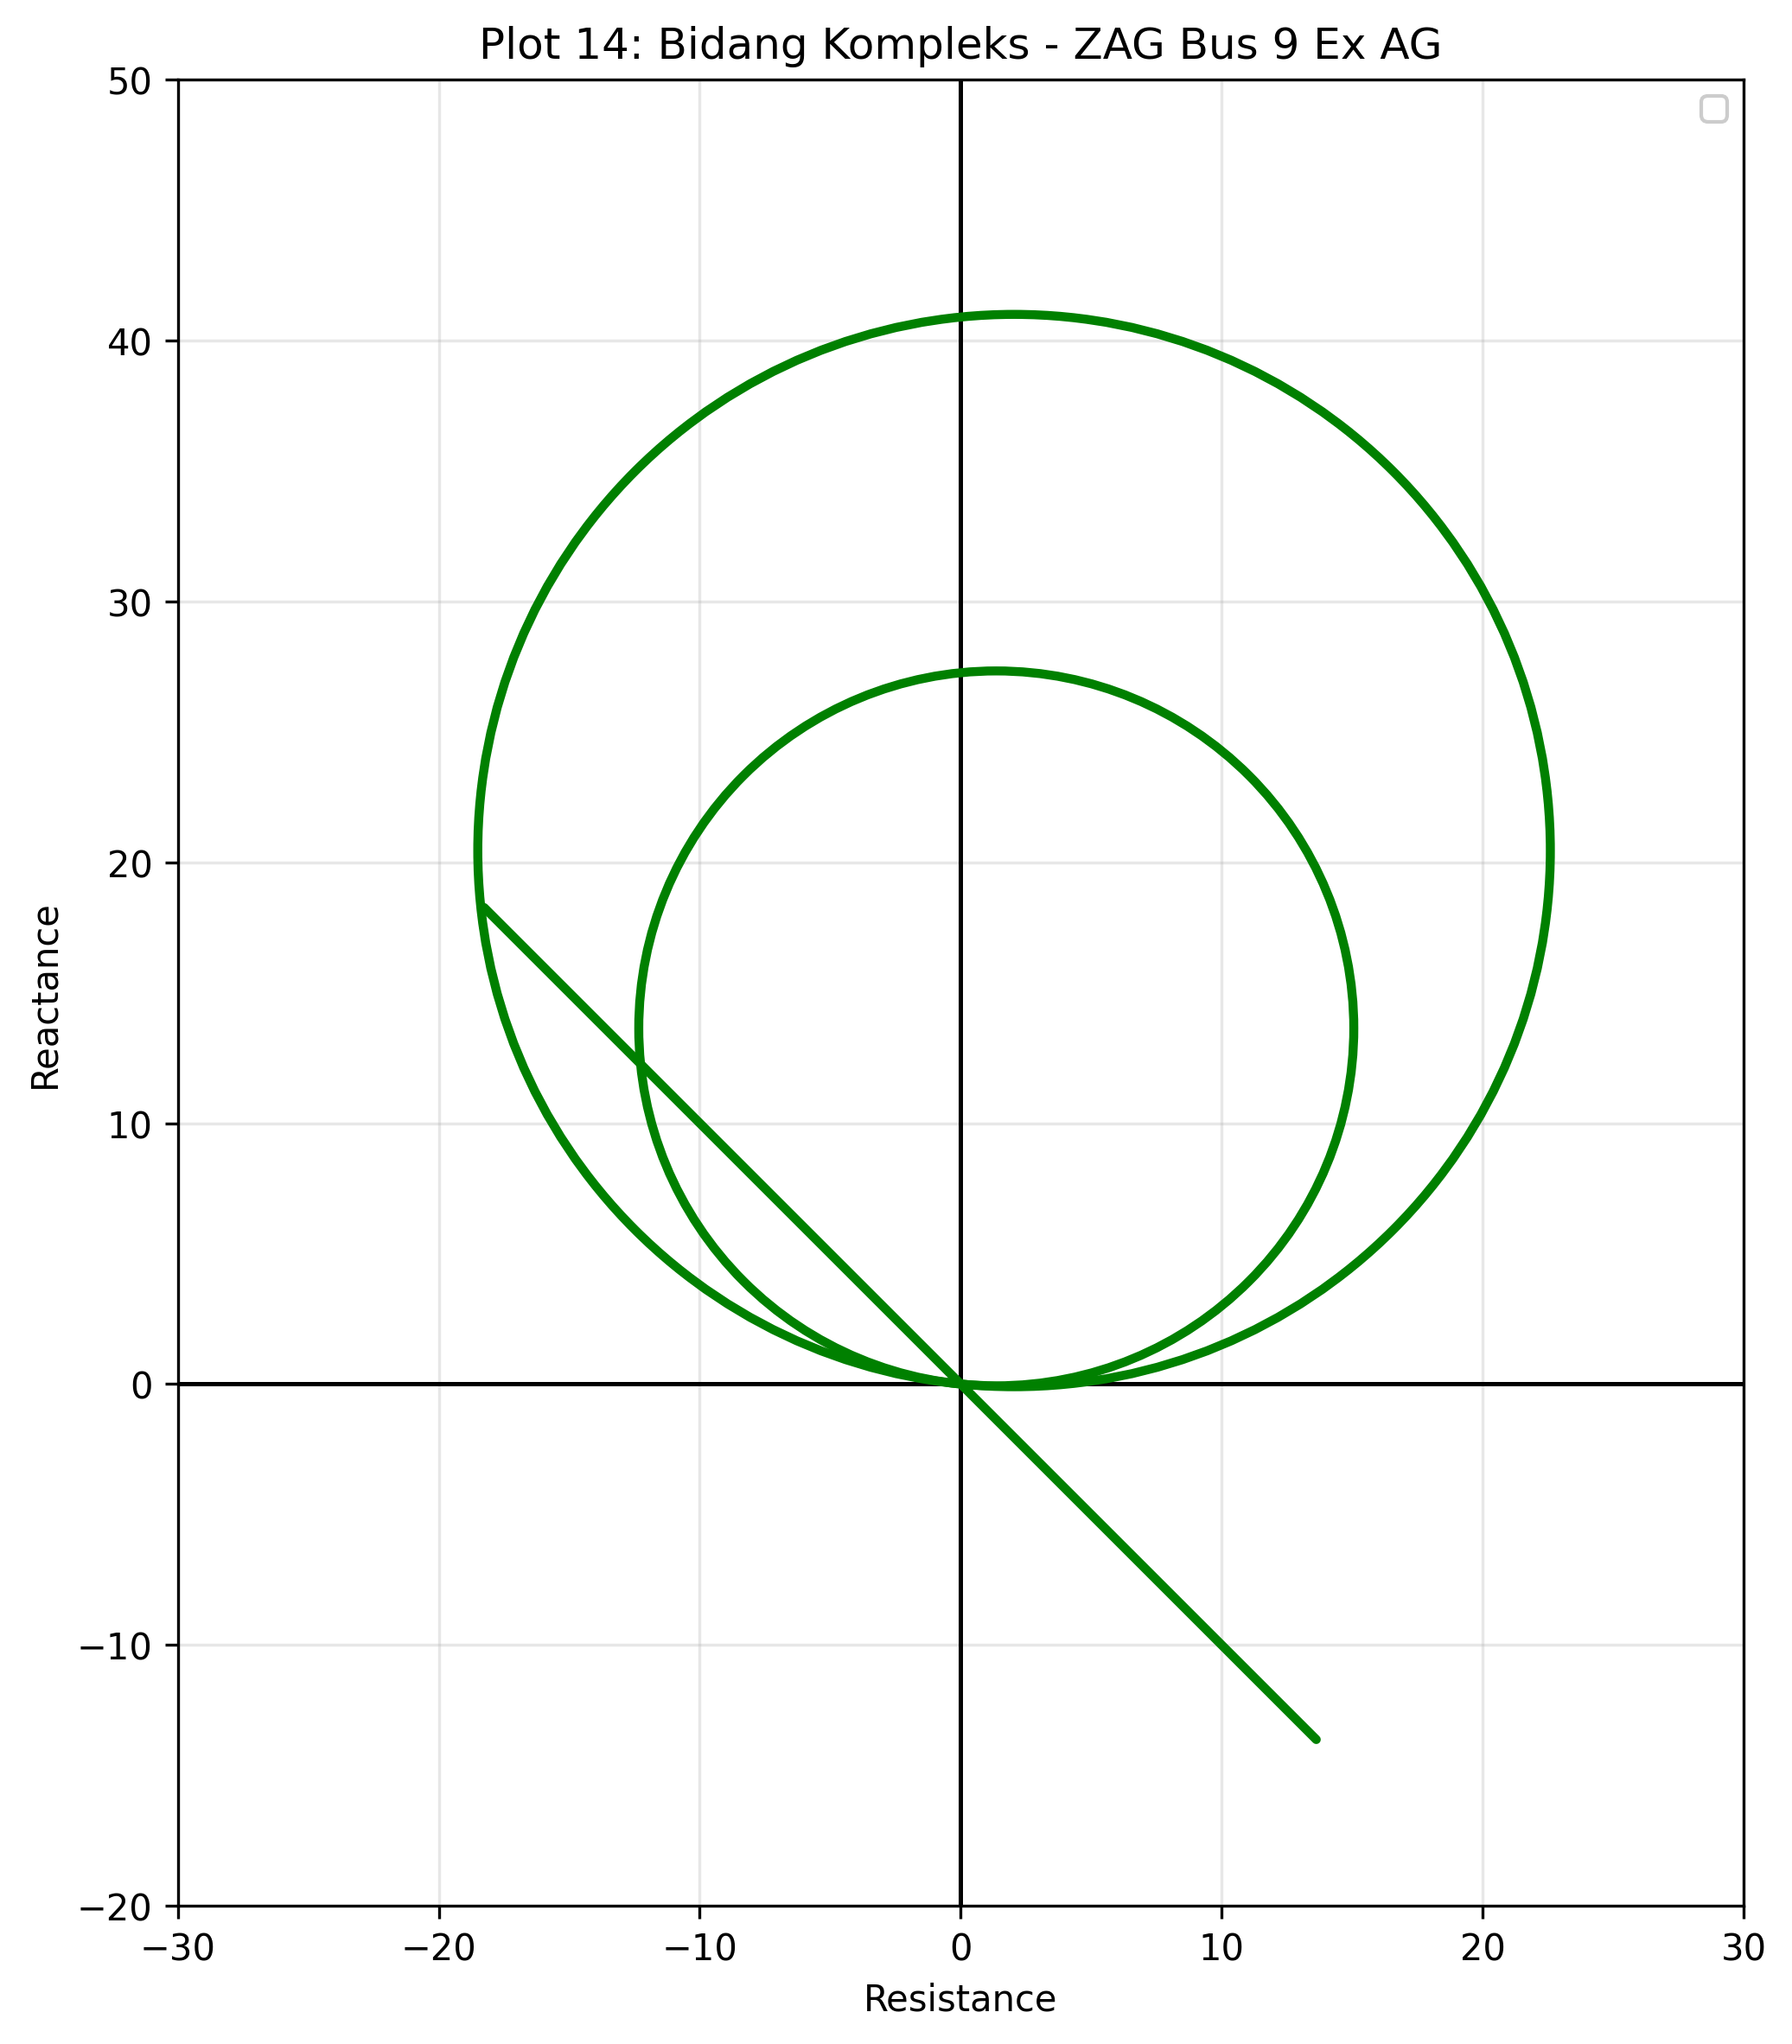
\includegraphics[width=0.8\textwidth]{contents/chapter-4/TIBR_14_ZAG_Bus_9_Ex_AG.png}
    \caption{Impedansi Tampak ZAG Bus 9 External SLG Fault}
    \label{fig:TIBR_14_ZAG_Bus_9_Ex_AG}
\end{figure}

Gambar \ref{fig:TIBR_14_ZAG_Bus_9_Ex_AG} menunjukkan impedansi tampak loop fasa A dengan ground yang dibaca oleh relay 21 melalui CT dan VT pada Bus 9. Pada sisi ini, relay tidak mendeteksi gangguan eksternal SLG sebagai gangguan yang perlu dioperasikan. Dengan demikian, relay 21 sisi Bus 9 tidak mengirimkan sinyal trip kepada CB dan responsnya tetap sesuai untuk gangguan eksternal.

\begin{figure}[H]
    \centering
    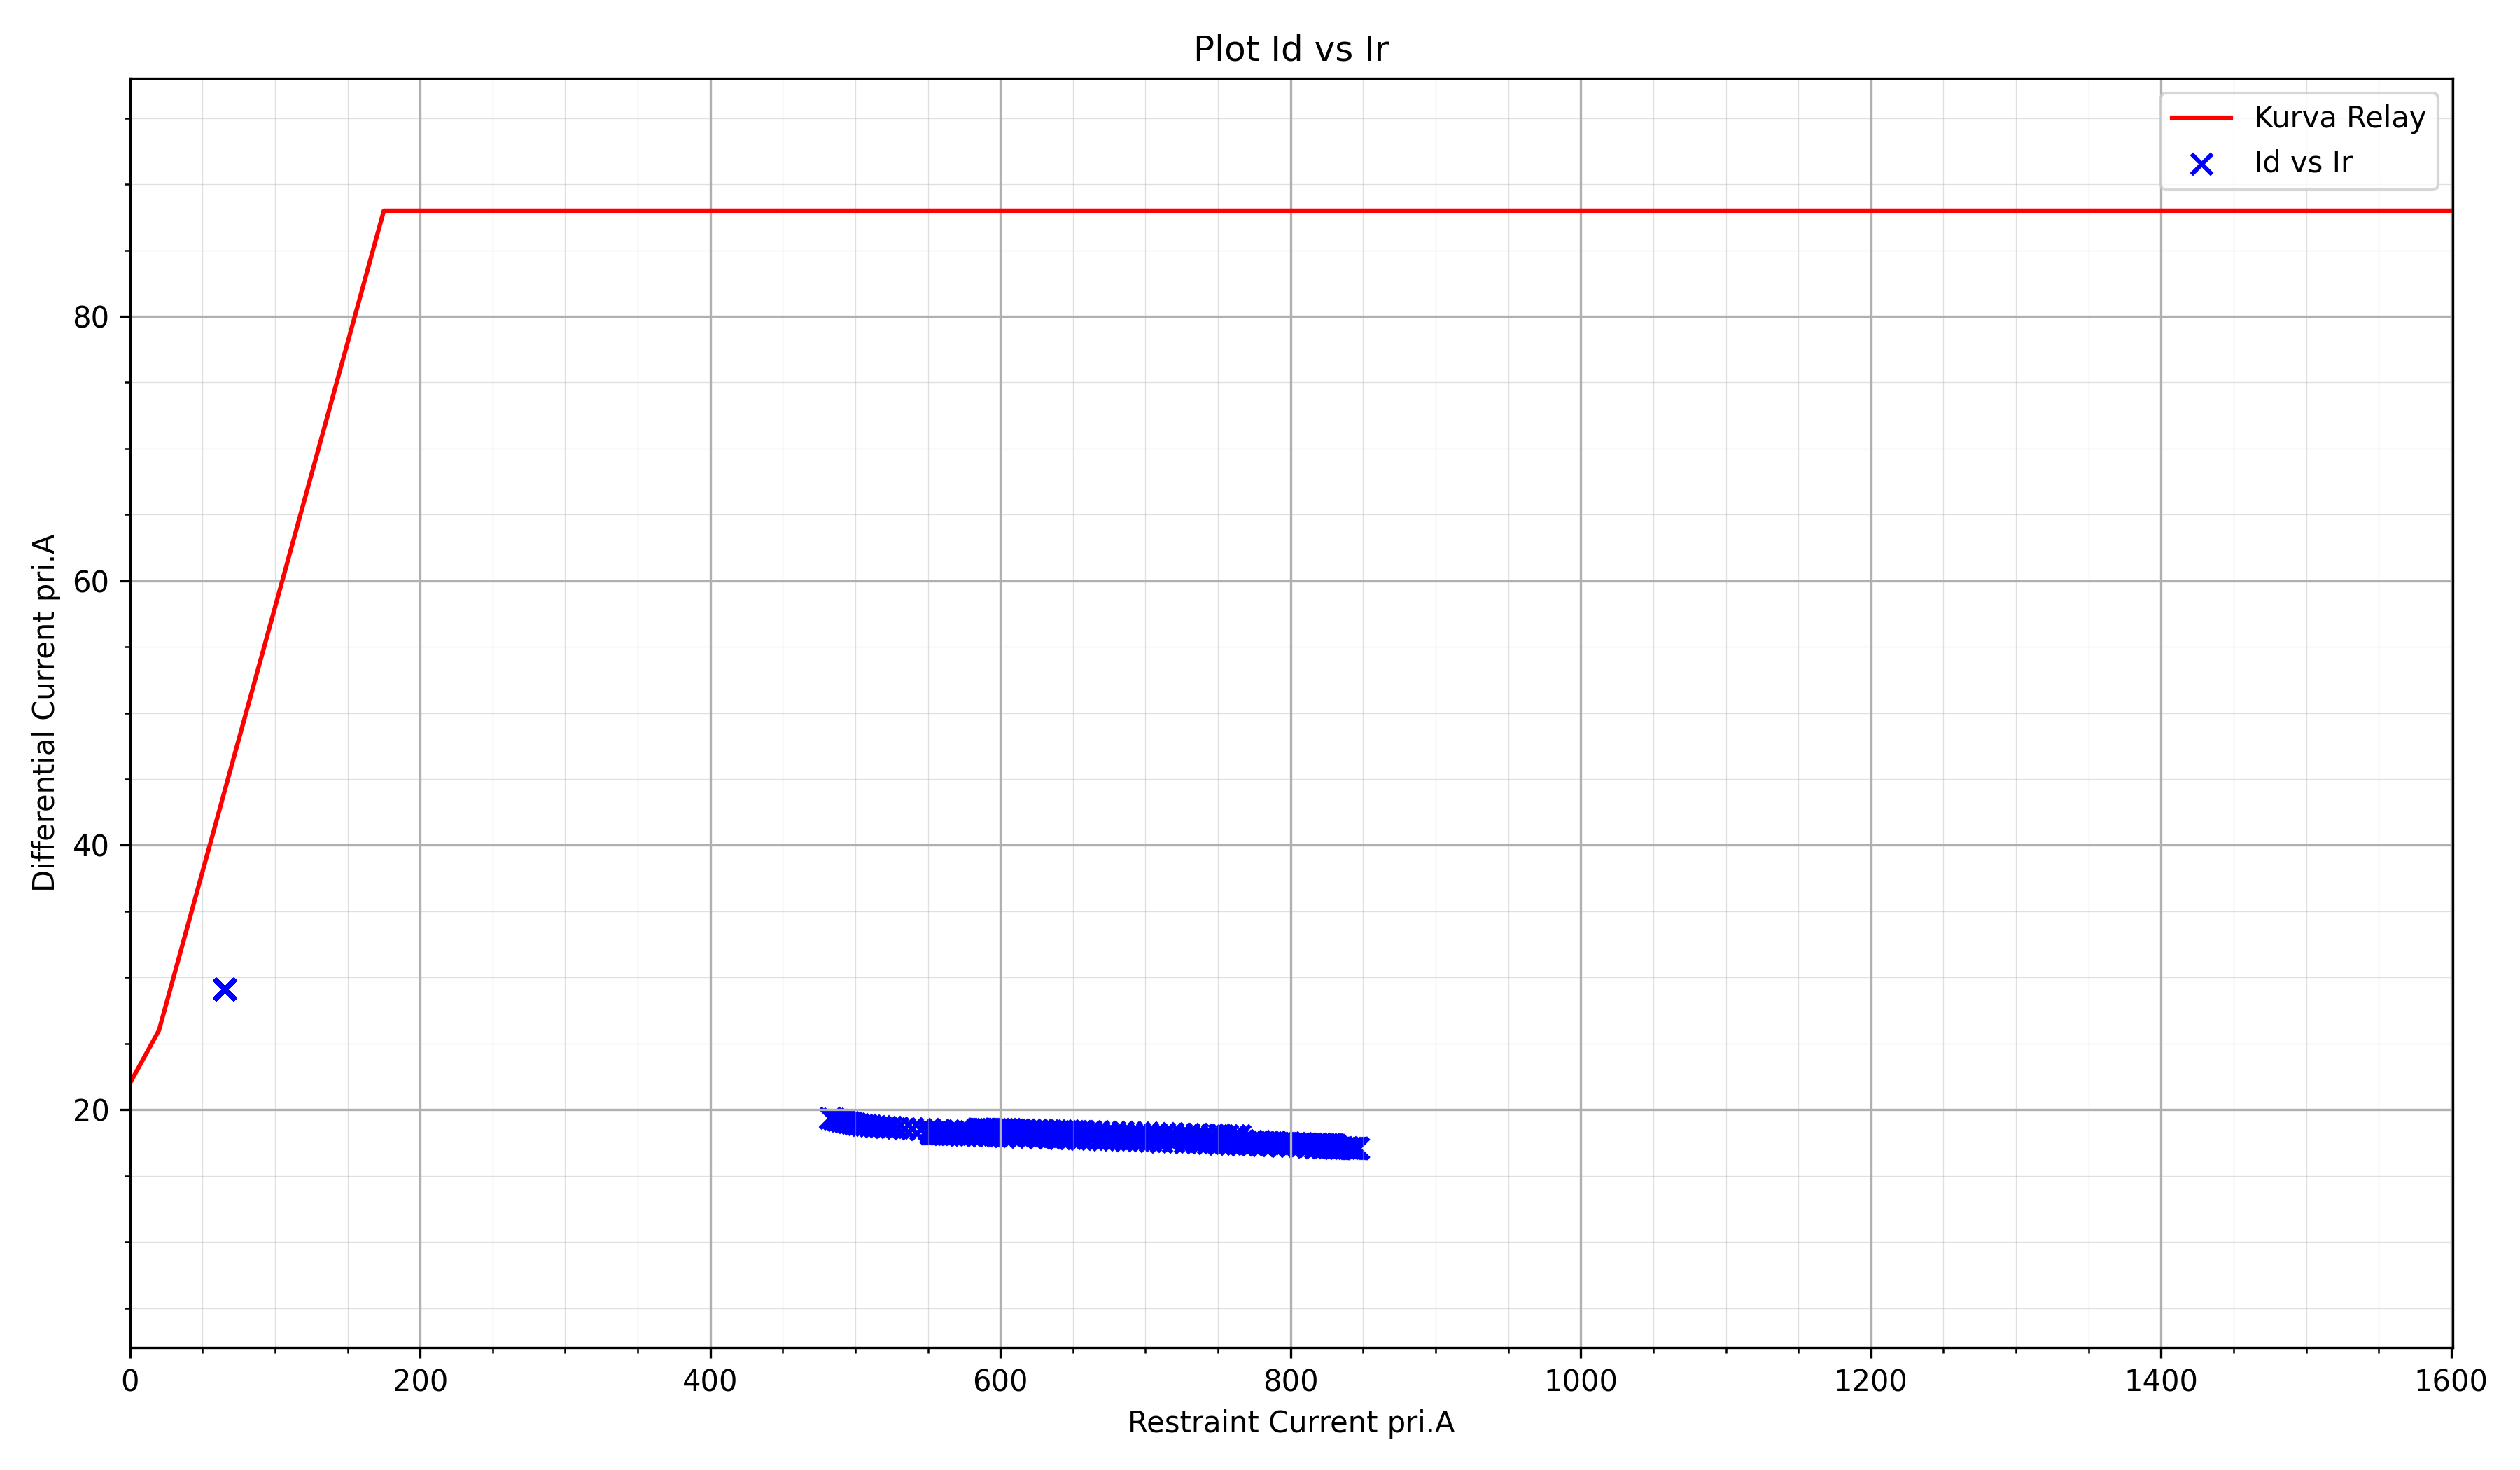
\includegraphics[width=0.8\textwidth]{contents/chapter-4/87LTIBR_plot_Ax3_Ay3.png}
    \caption{Current Comparison Differential Fasa A External SLG Fault}
    \label{fig:87LTIBR_plot_Ax3_Ay3}
\end{figure}

Gambar \ref{fig:87LTIBR_plot_Ax3_Ay3} menunjukkan plot \textit{current comparison differential} pada fasa A saat terjadi gangguan eksternal SLG. Titik arus berada di bawah batas operasi yang ditentukan oleh setting relay. Kondisi ini menyebabkan relay 87L tetap berada pada daerah penahan, sehingga relay tidak memerintahkan trip pada CB.

\begin{figure}[H]
    \centering
    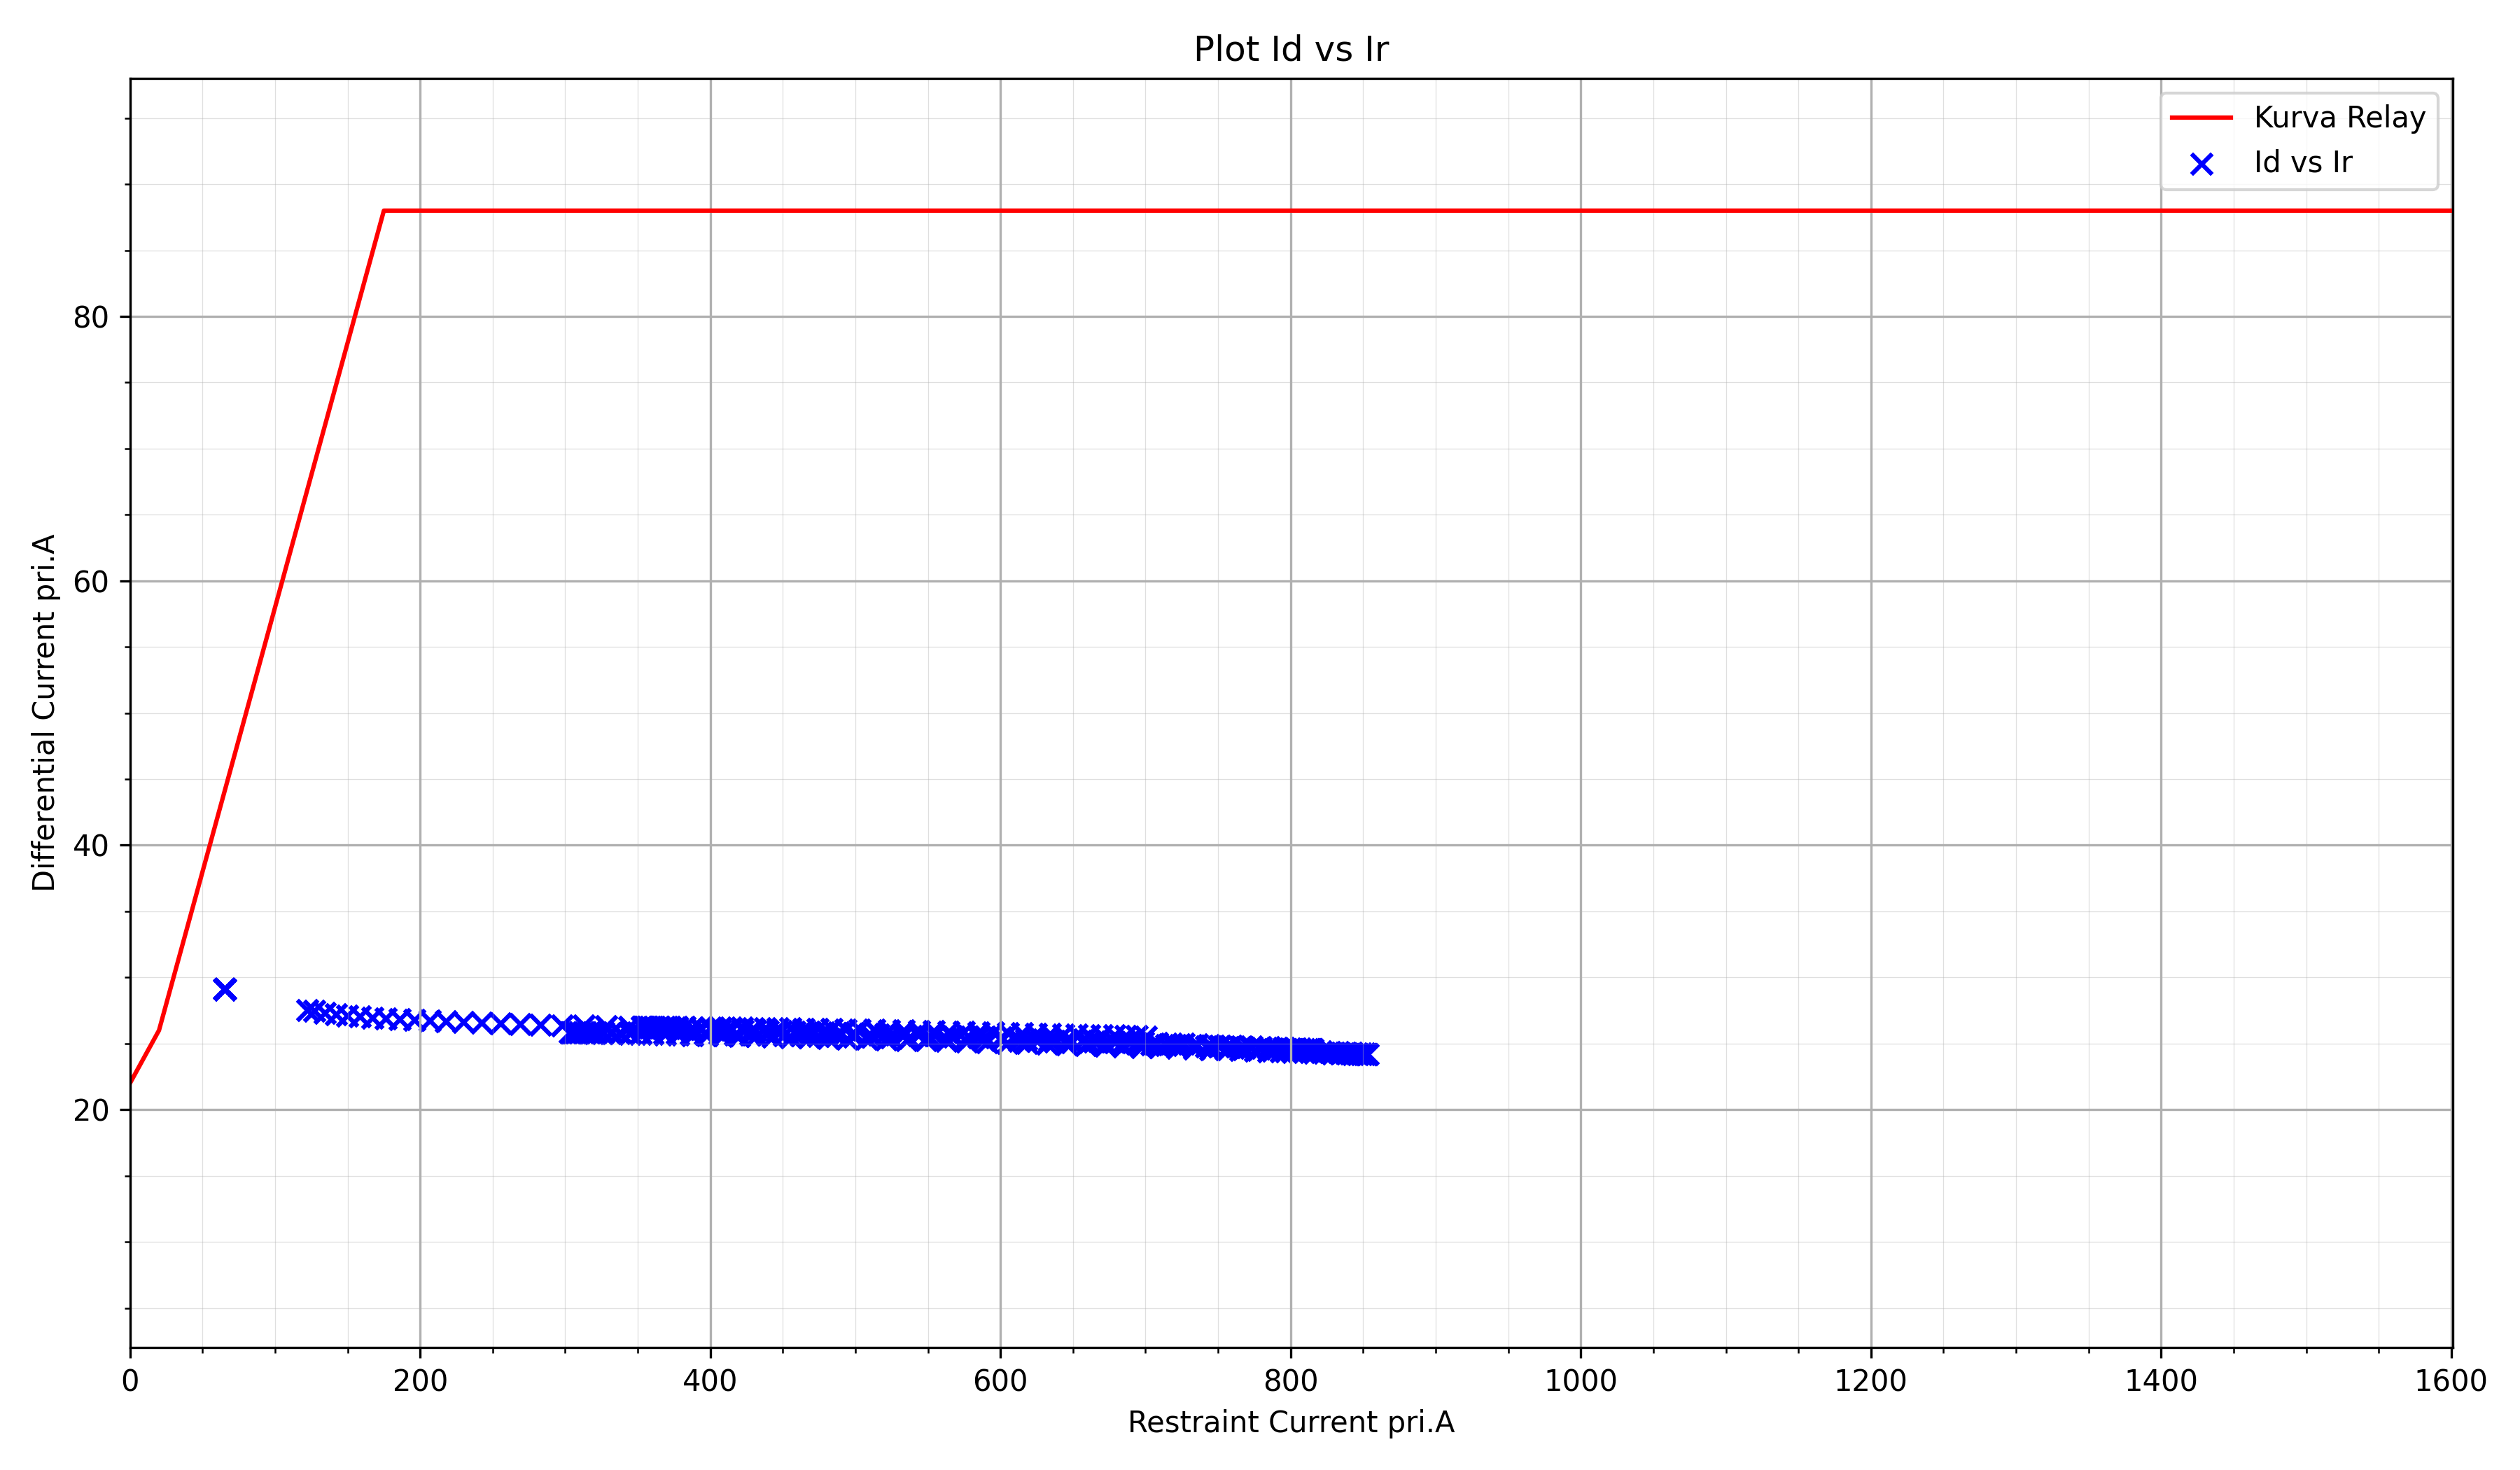
\includegraphics[width=0.8\textwidth]{contents/chapter-4/87LTIBR_plot_Bx3_By3.png}
    \caption{Current Comparison Differential Fasa B External SLG Fault}
    \label{fig:87LTIBR_plot_Bx3_By3}
\end{figure}

Gambar \ref{fig:87LTIBR_plot_Bx3_By3} menunjukkan plot \textit{current comparison differential} pada fasa B saat terjadi gangguan eksternal SLG. Pada plot tersebut, titik arus masih berada di bawah batas operasi relay. Dengan posisi ini, relay 87L tidak membaca adanya gangguan internal dan tidak memberikan perintah trip kepada CB.

\begin{figure}[H]
    \centering
    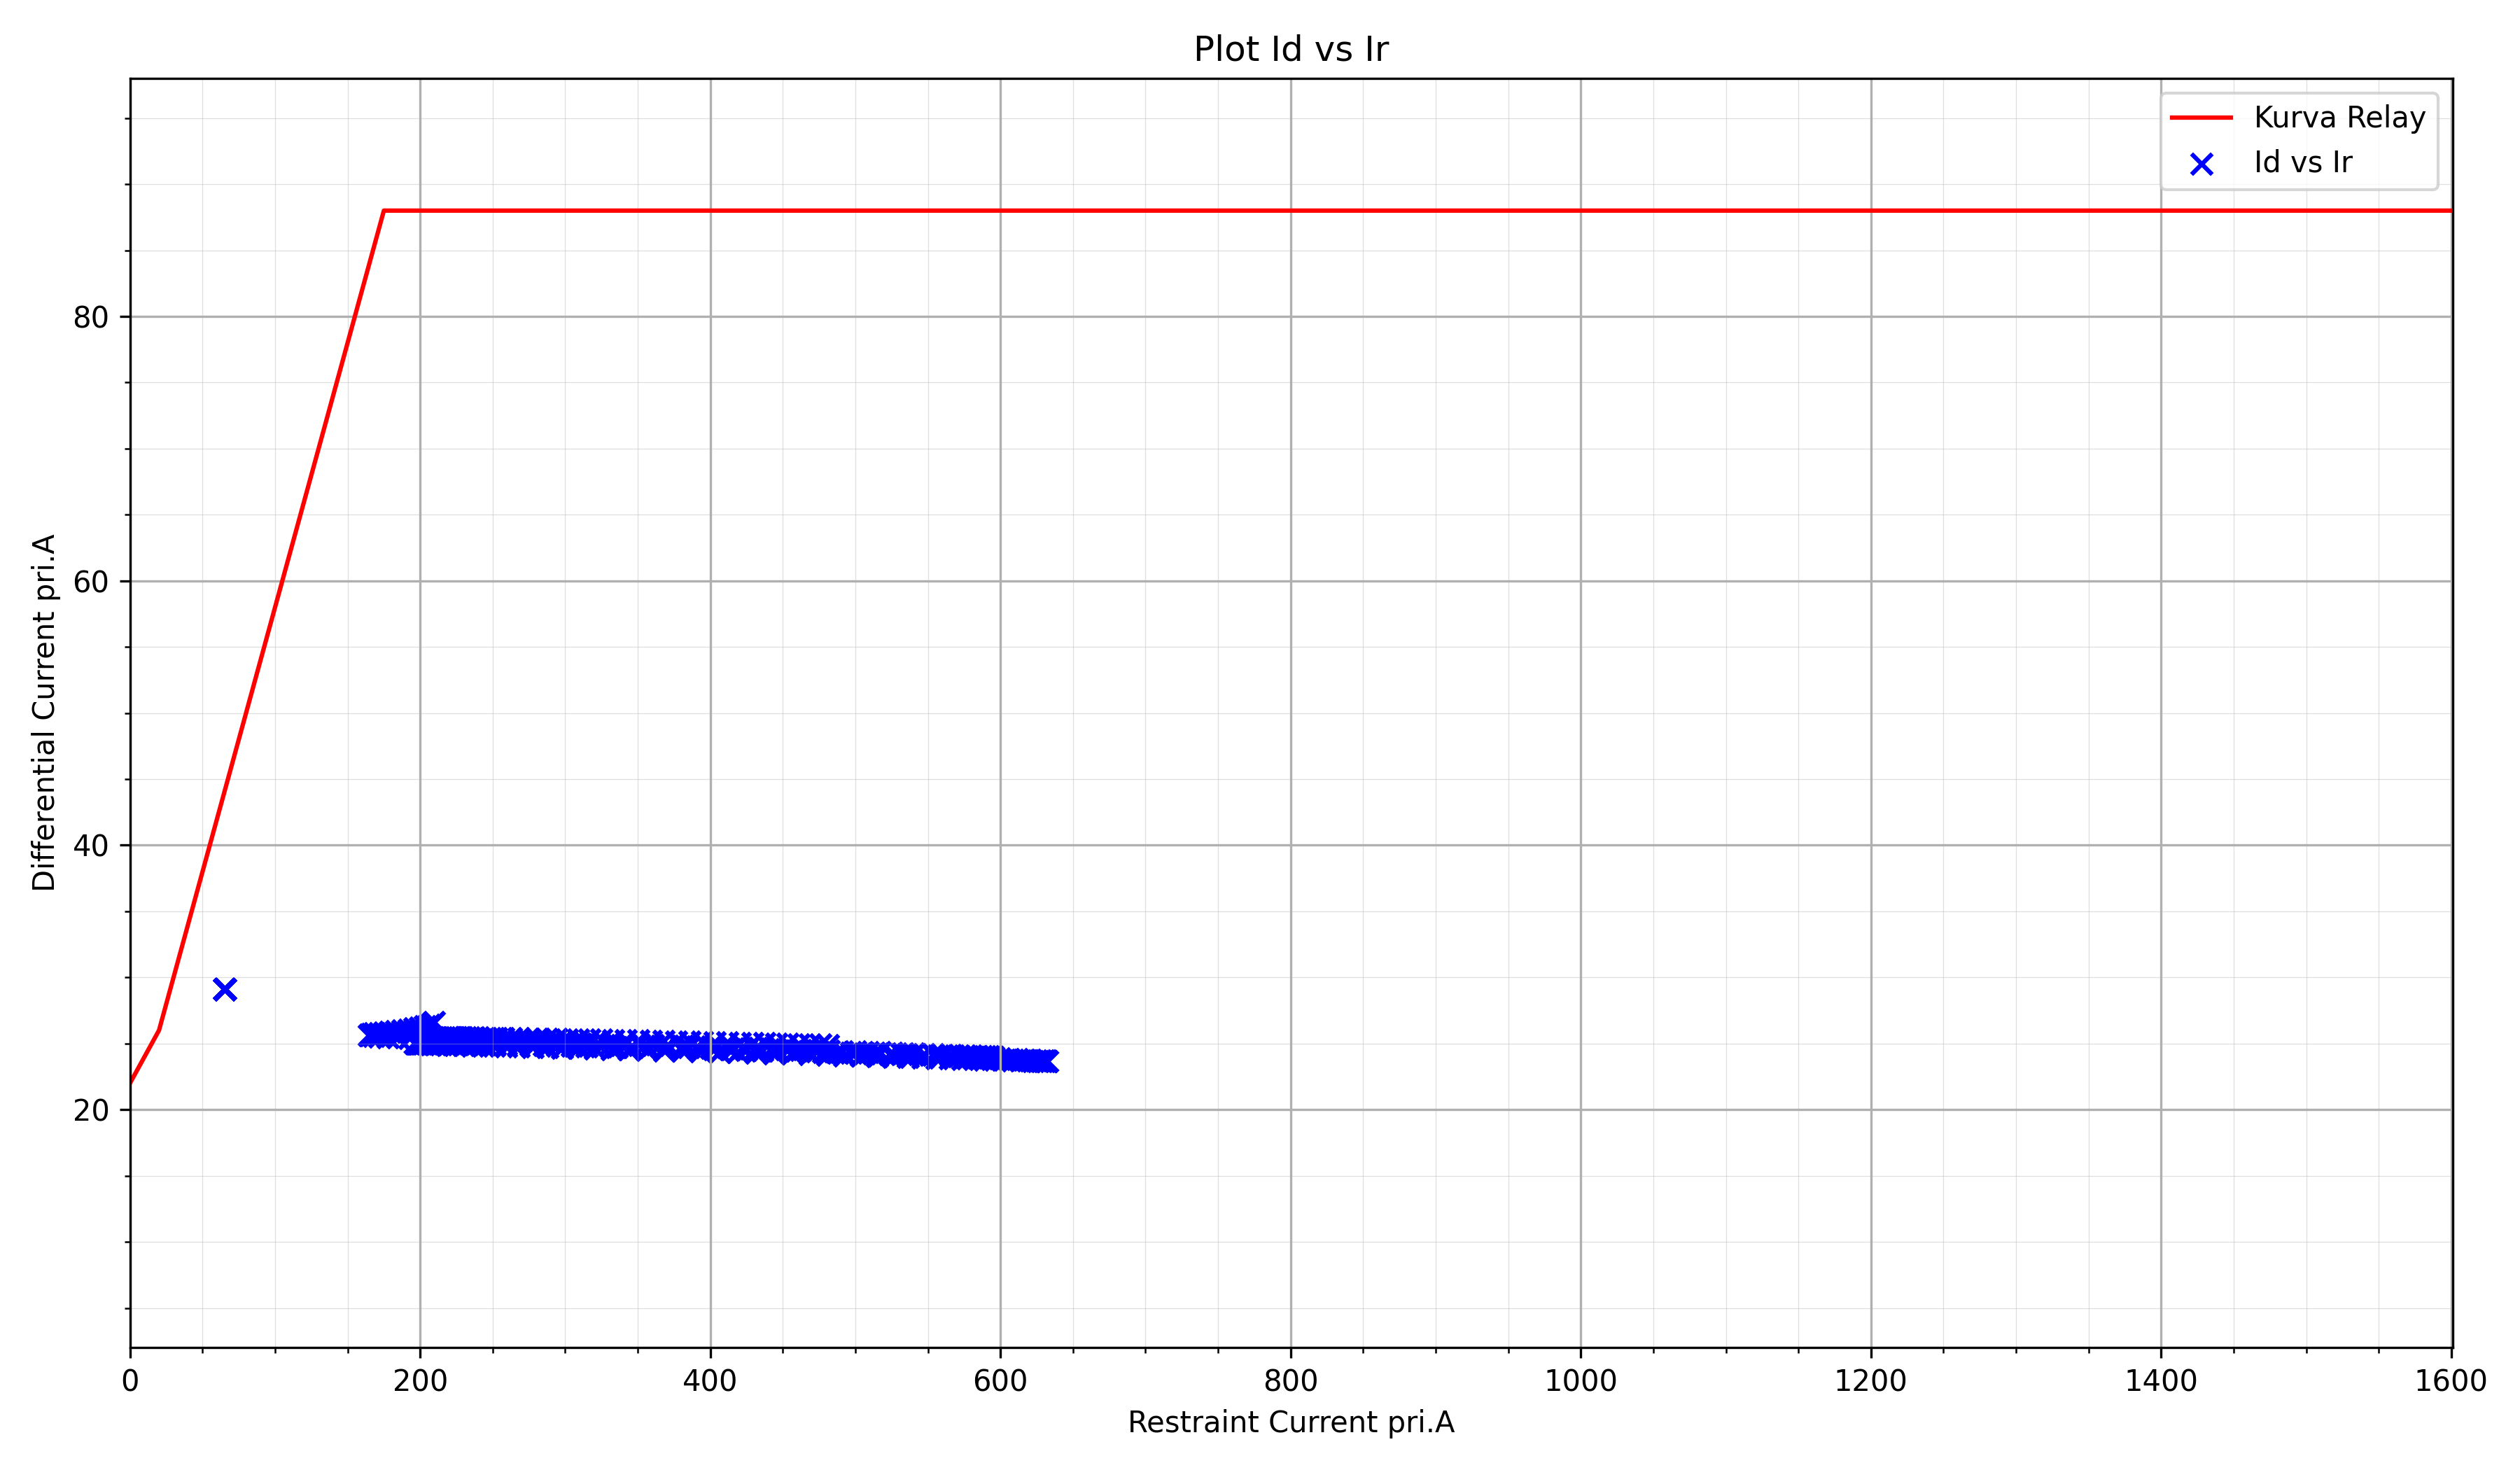
\includegraphics[width=0.8\textwidth]{contents/chapter-4/87LTIBR_plot_Cx3_Cy3.png}
    \caption{Current Comparison Differential Fasa C External SLG Fault}
    \label{fig:87LTIBR_plot_Cx3_Cy3}
\end{figure}

Gambar \ref{fig:87LTIBR_plot_Cx3_Cy3} menunjukkan plot \textit{current comparison differential} pada fasa C saat terjadi gangguan eksternal SLG. Titik arus pada fasa C juga berada di bawah batas operasi yang ditentukan oleh setting relay. Oleh karena itu, relay 87L tidak memerintahkan trip kepada CB dan tetap menunjukkan respons penahan untuk gangguan eksternal.

\subsection{Respons Relay terhadap gangguan External Double Line to Ground (DLG)}
\label{subsec:tanpa_IBR_ex_dlg}

\begin{figure}[H]
    \centering
    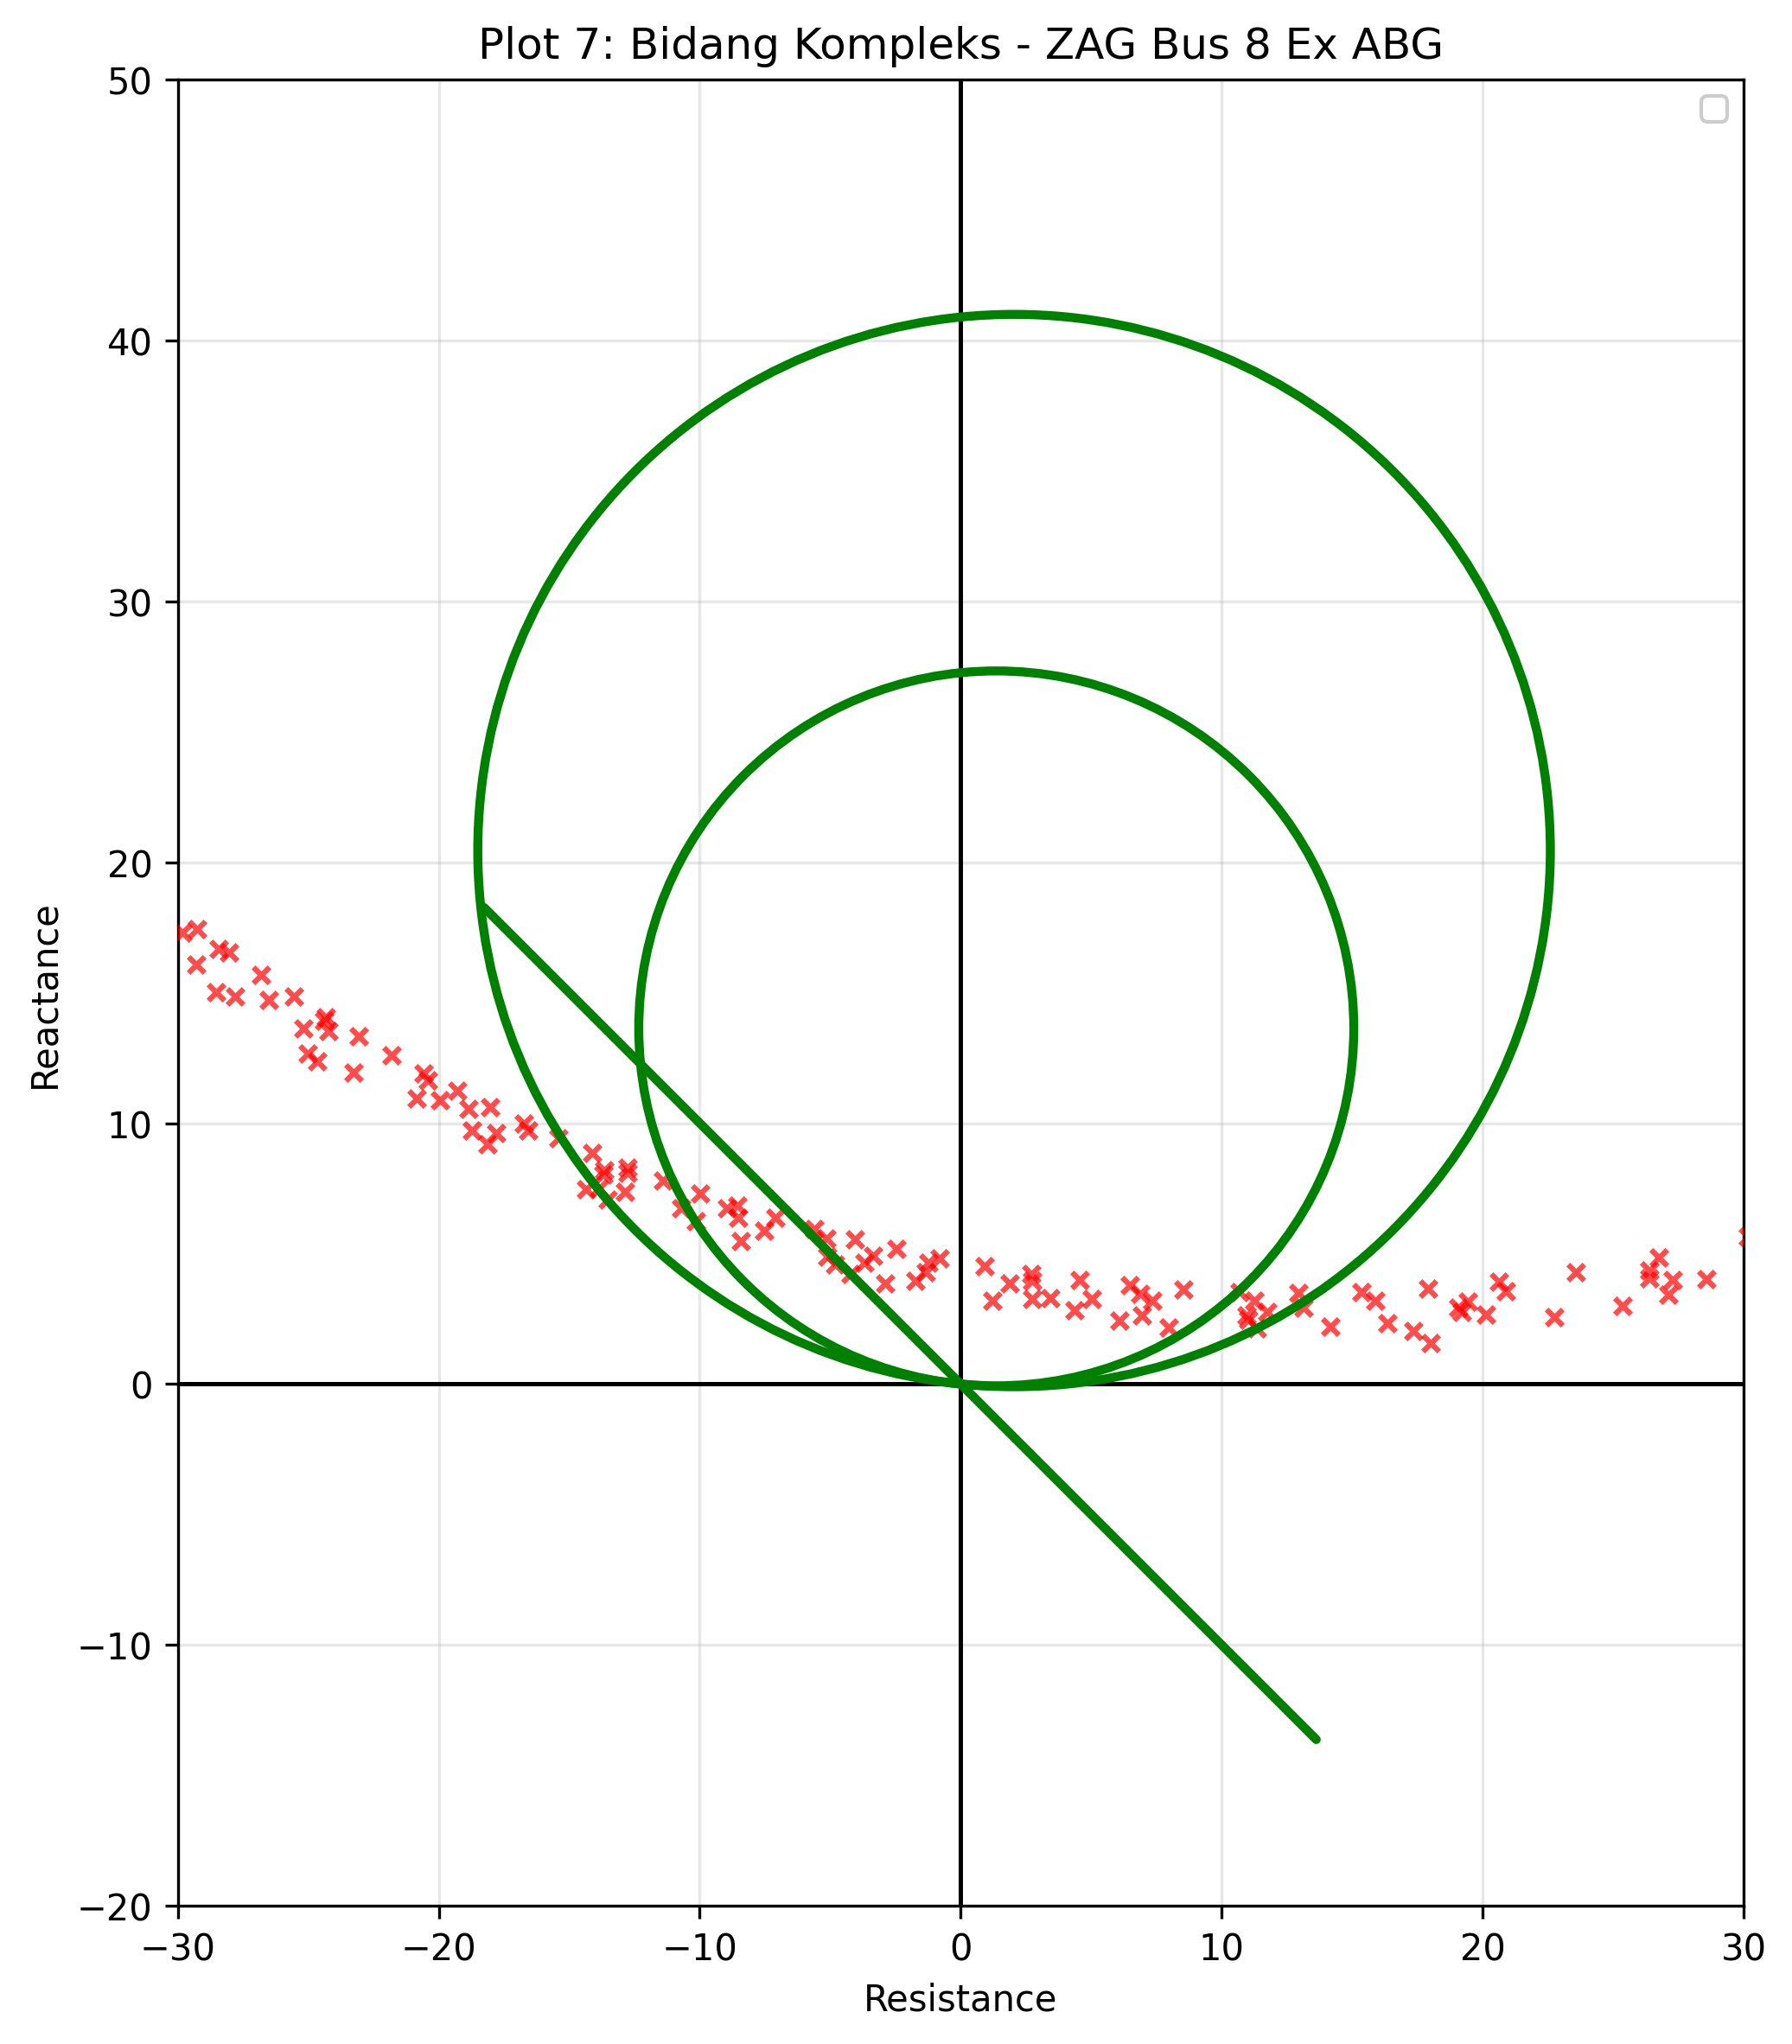
\includegraphics[width=0.8\textwidth]{contents/chapter-4/TIBR_07_ZAG_Bus_8_Ex_ABG.png}
    \caption{Impedansi Tampak ZAG Bus 8 External DLG Fault}
    \label{fig:TIBR_07_ZAG_Bus_8_Ex_ABG}
\end{figure}

\begin{figure}[H]
    \centering
    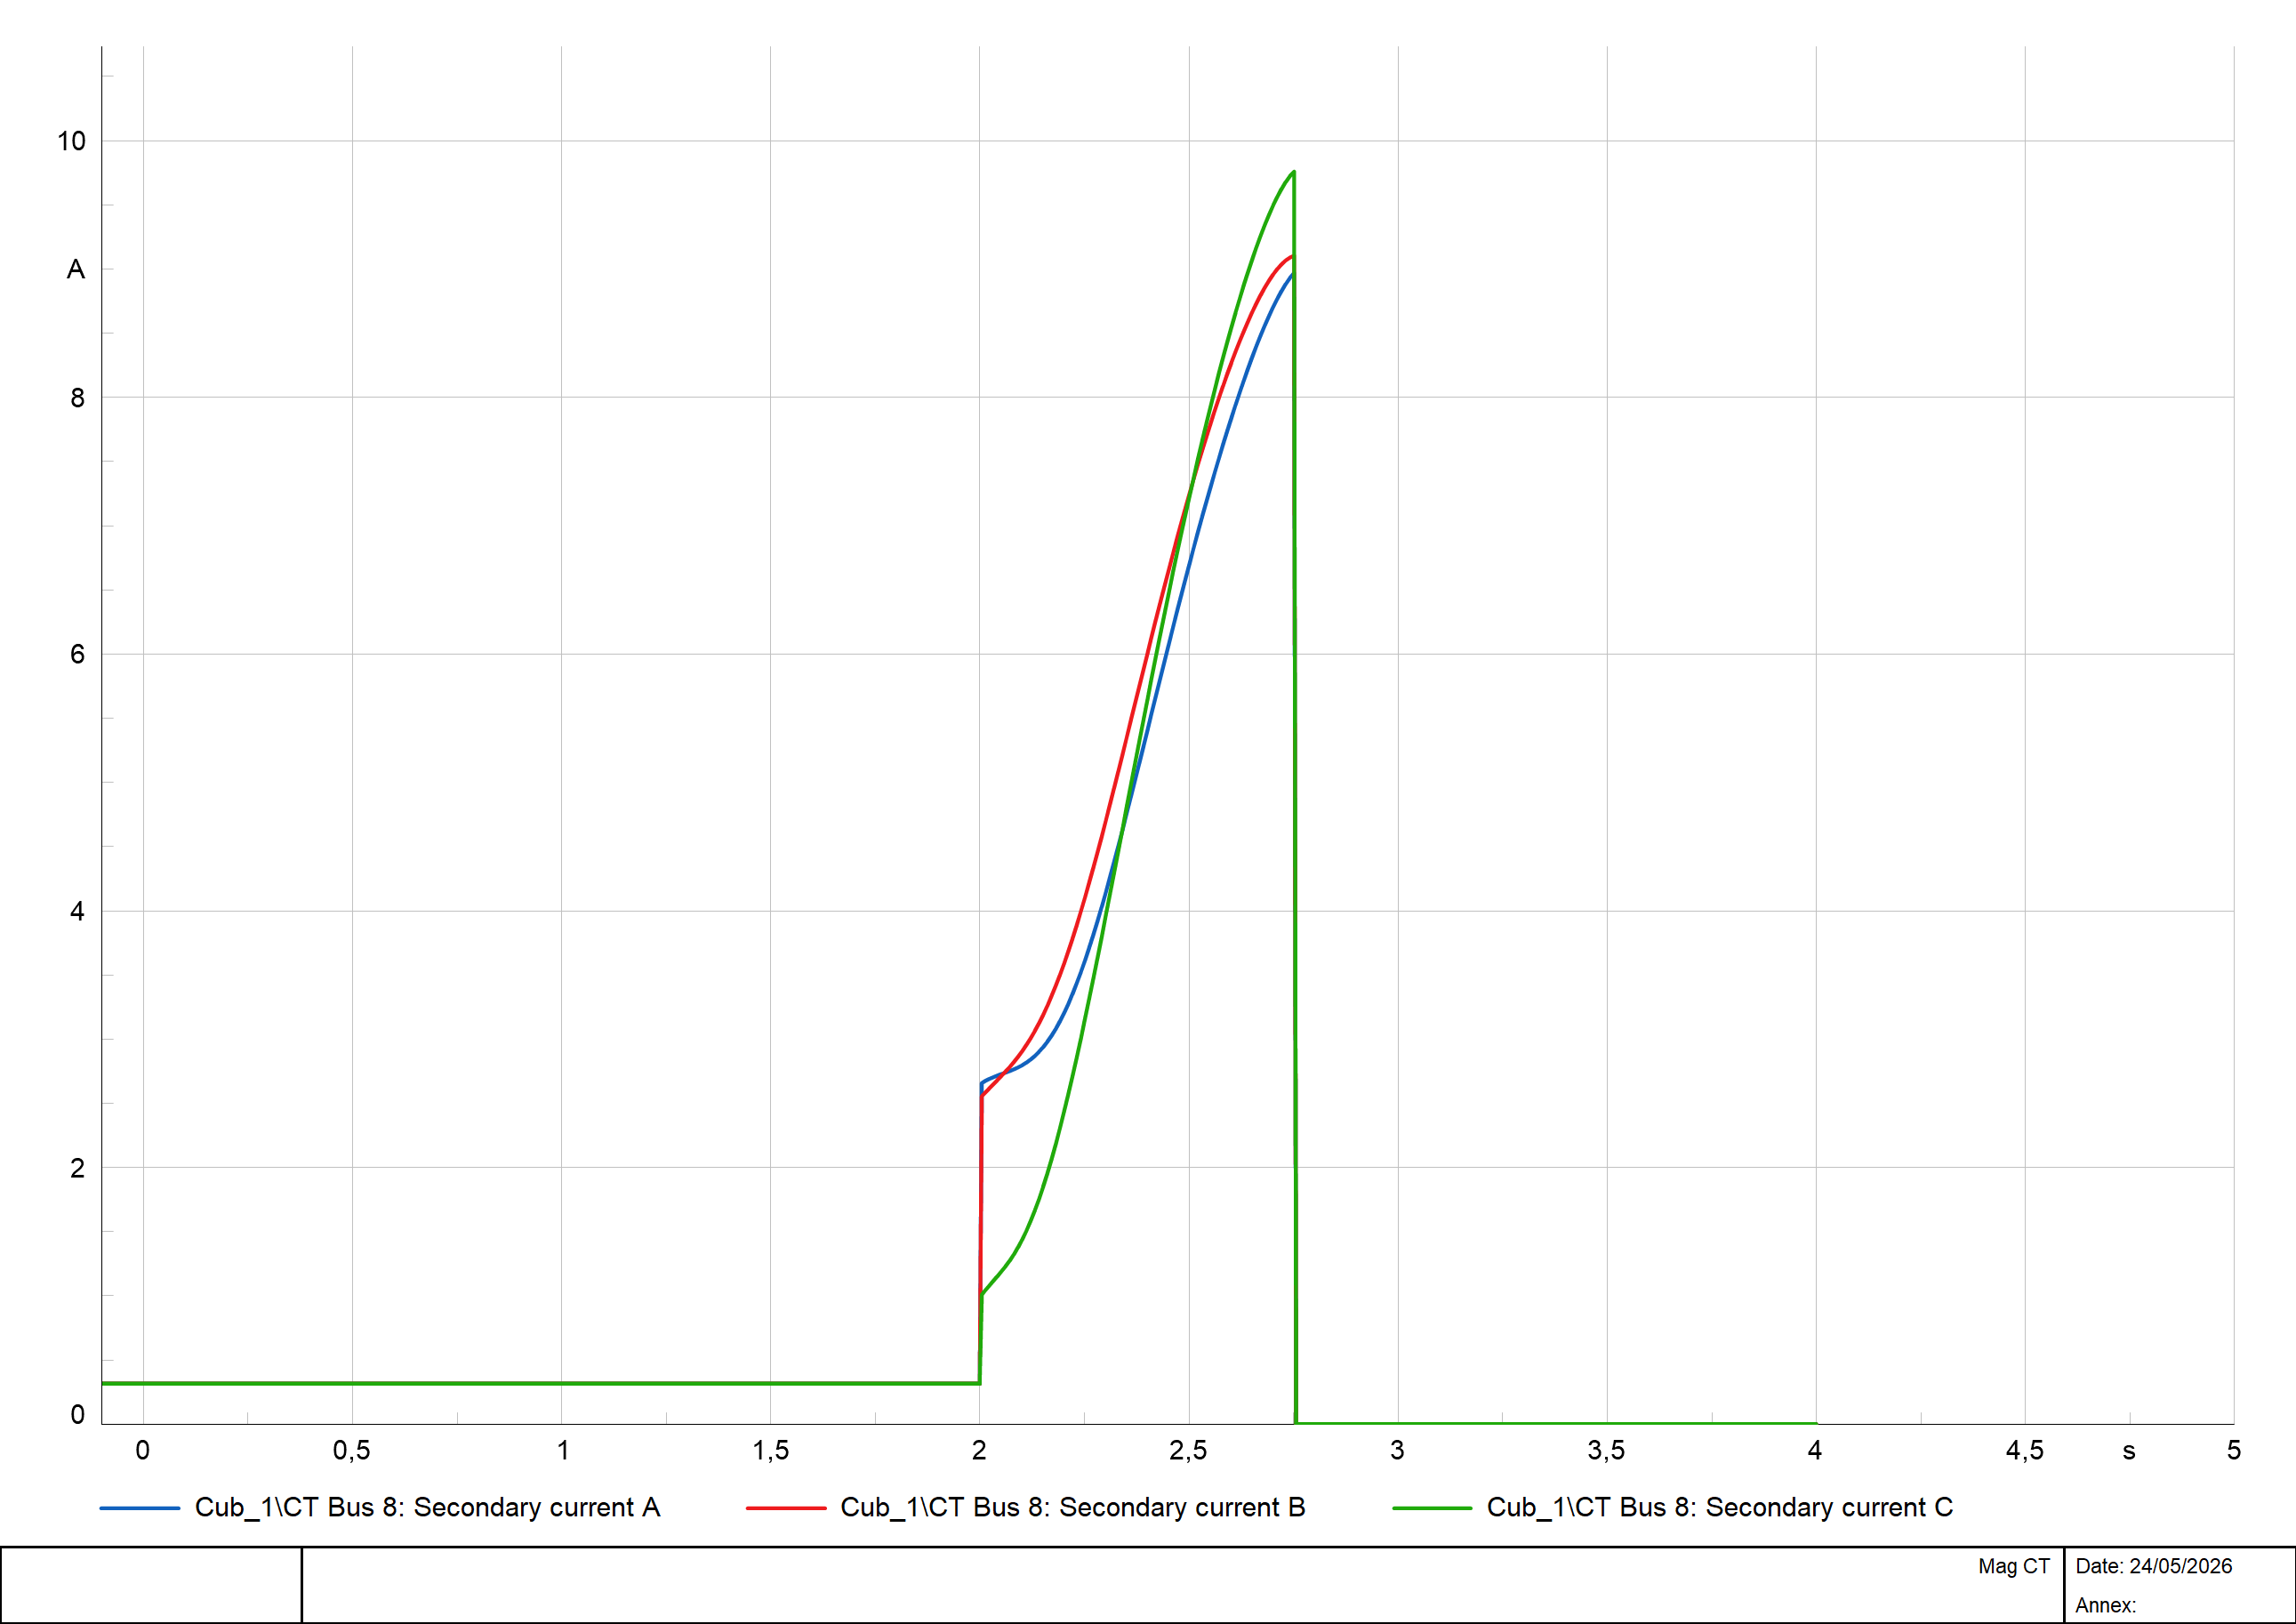
\includegraphics[width=0.8\textwidth]{contents/chapter-4/Bus_8_Ex_DLG.png}
    \caption{Arus Sekunder CT Bus 8 Pada External DLG Fault}
    \label{fig:Bus_8_Ex_DLG}
\end{figure}

Gambar \ref{fig:TIBR_07_ZAG_Bus_8_Ex_ABG} menunjukkan impedansi tampak loop fasa A dengan ground yang dibaca oleh relay 21 melalui CT dan VT pada Bus 8. Hasil plot menunjukkan bahwa saat terjadi gangguan eksternal DLG, impedansi tampak yang dibaca relay masuk ke dalam zona 1. Relay memberikan perintah trip karena arus yang mengalir sudah membuat relay aktif dan melebihi batas arus maksimum untuk trip instan, sebagaimana ditunjukkan pada Gambar \ref{fig:Bus_8_Ex_DLG}.

\begin{figure}[H]
    \centering
    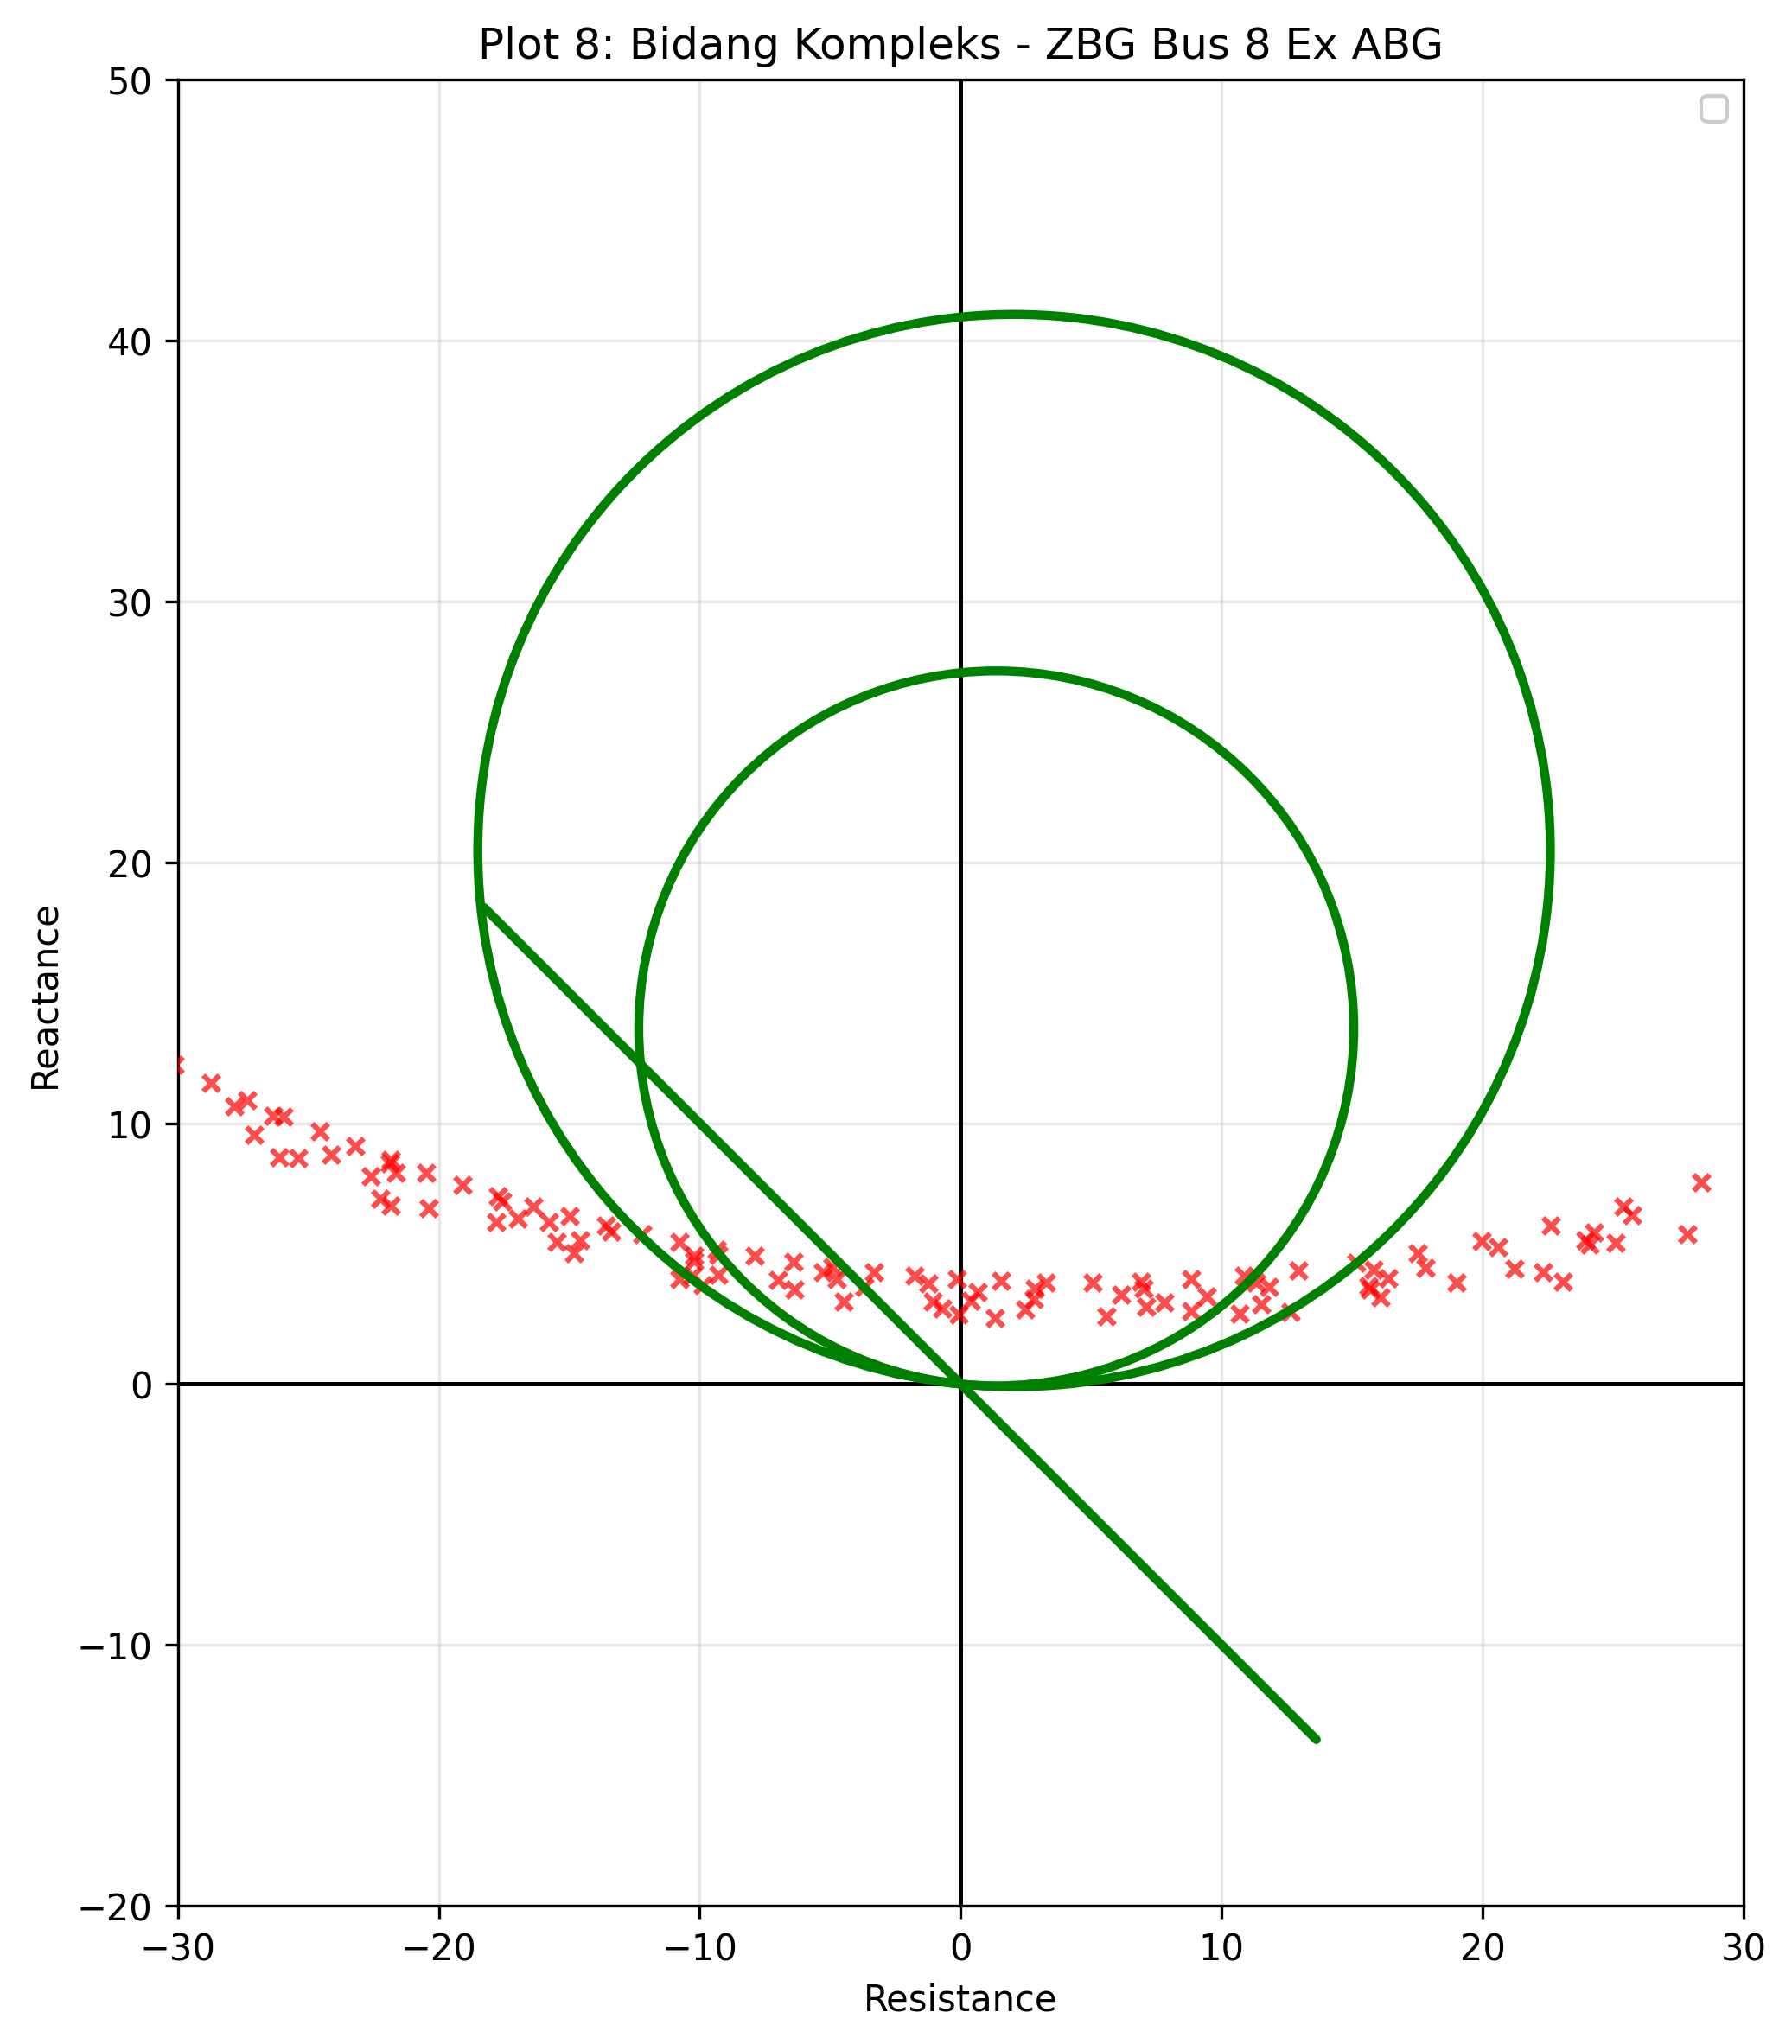
\includegraphics[width=0.8\textwidth]{contents/chapter-4/TIBR_08_ZBG_Bus_8_Ex_ABG.png}
    \caption{Impedansi Tampak ZBG Bus 8 External DLG Fault}
    \label{fig:TIBR_08_ZBG_Bus_8_Ex_ABG}
\end{figure}

Gambar \ref{fig:TIBR_08_ZBG_Bus_8_Ex_ABG} menunjukkan impedansi tampak loop fasa B dengan ground yang dibaca oleh relay 21 melalui CT dan VT pada Bus 8. Pada kondisi gangguan eksternal DLG, impedansi tampak yang dibaca relay masuk ke dalam zona 1. Relay tetap mengeluarkan perintah trip karena arus gangguan yang mengalir telah membuat relay aktif dan melebihi batas arus maksimum untuk trip instan, sesuai dengan Gambar \ref{fig:Bus_8_Ex_DLG}.

\begin{figure}[H]
    \centering
    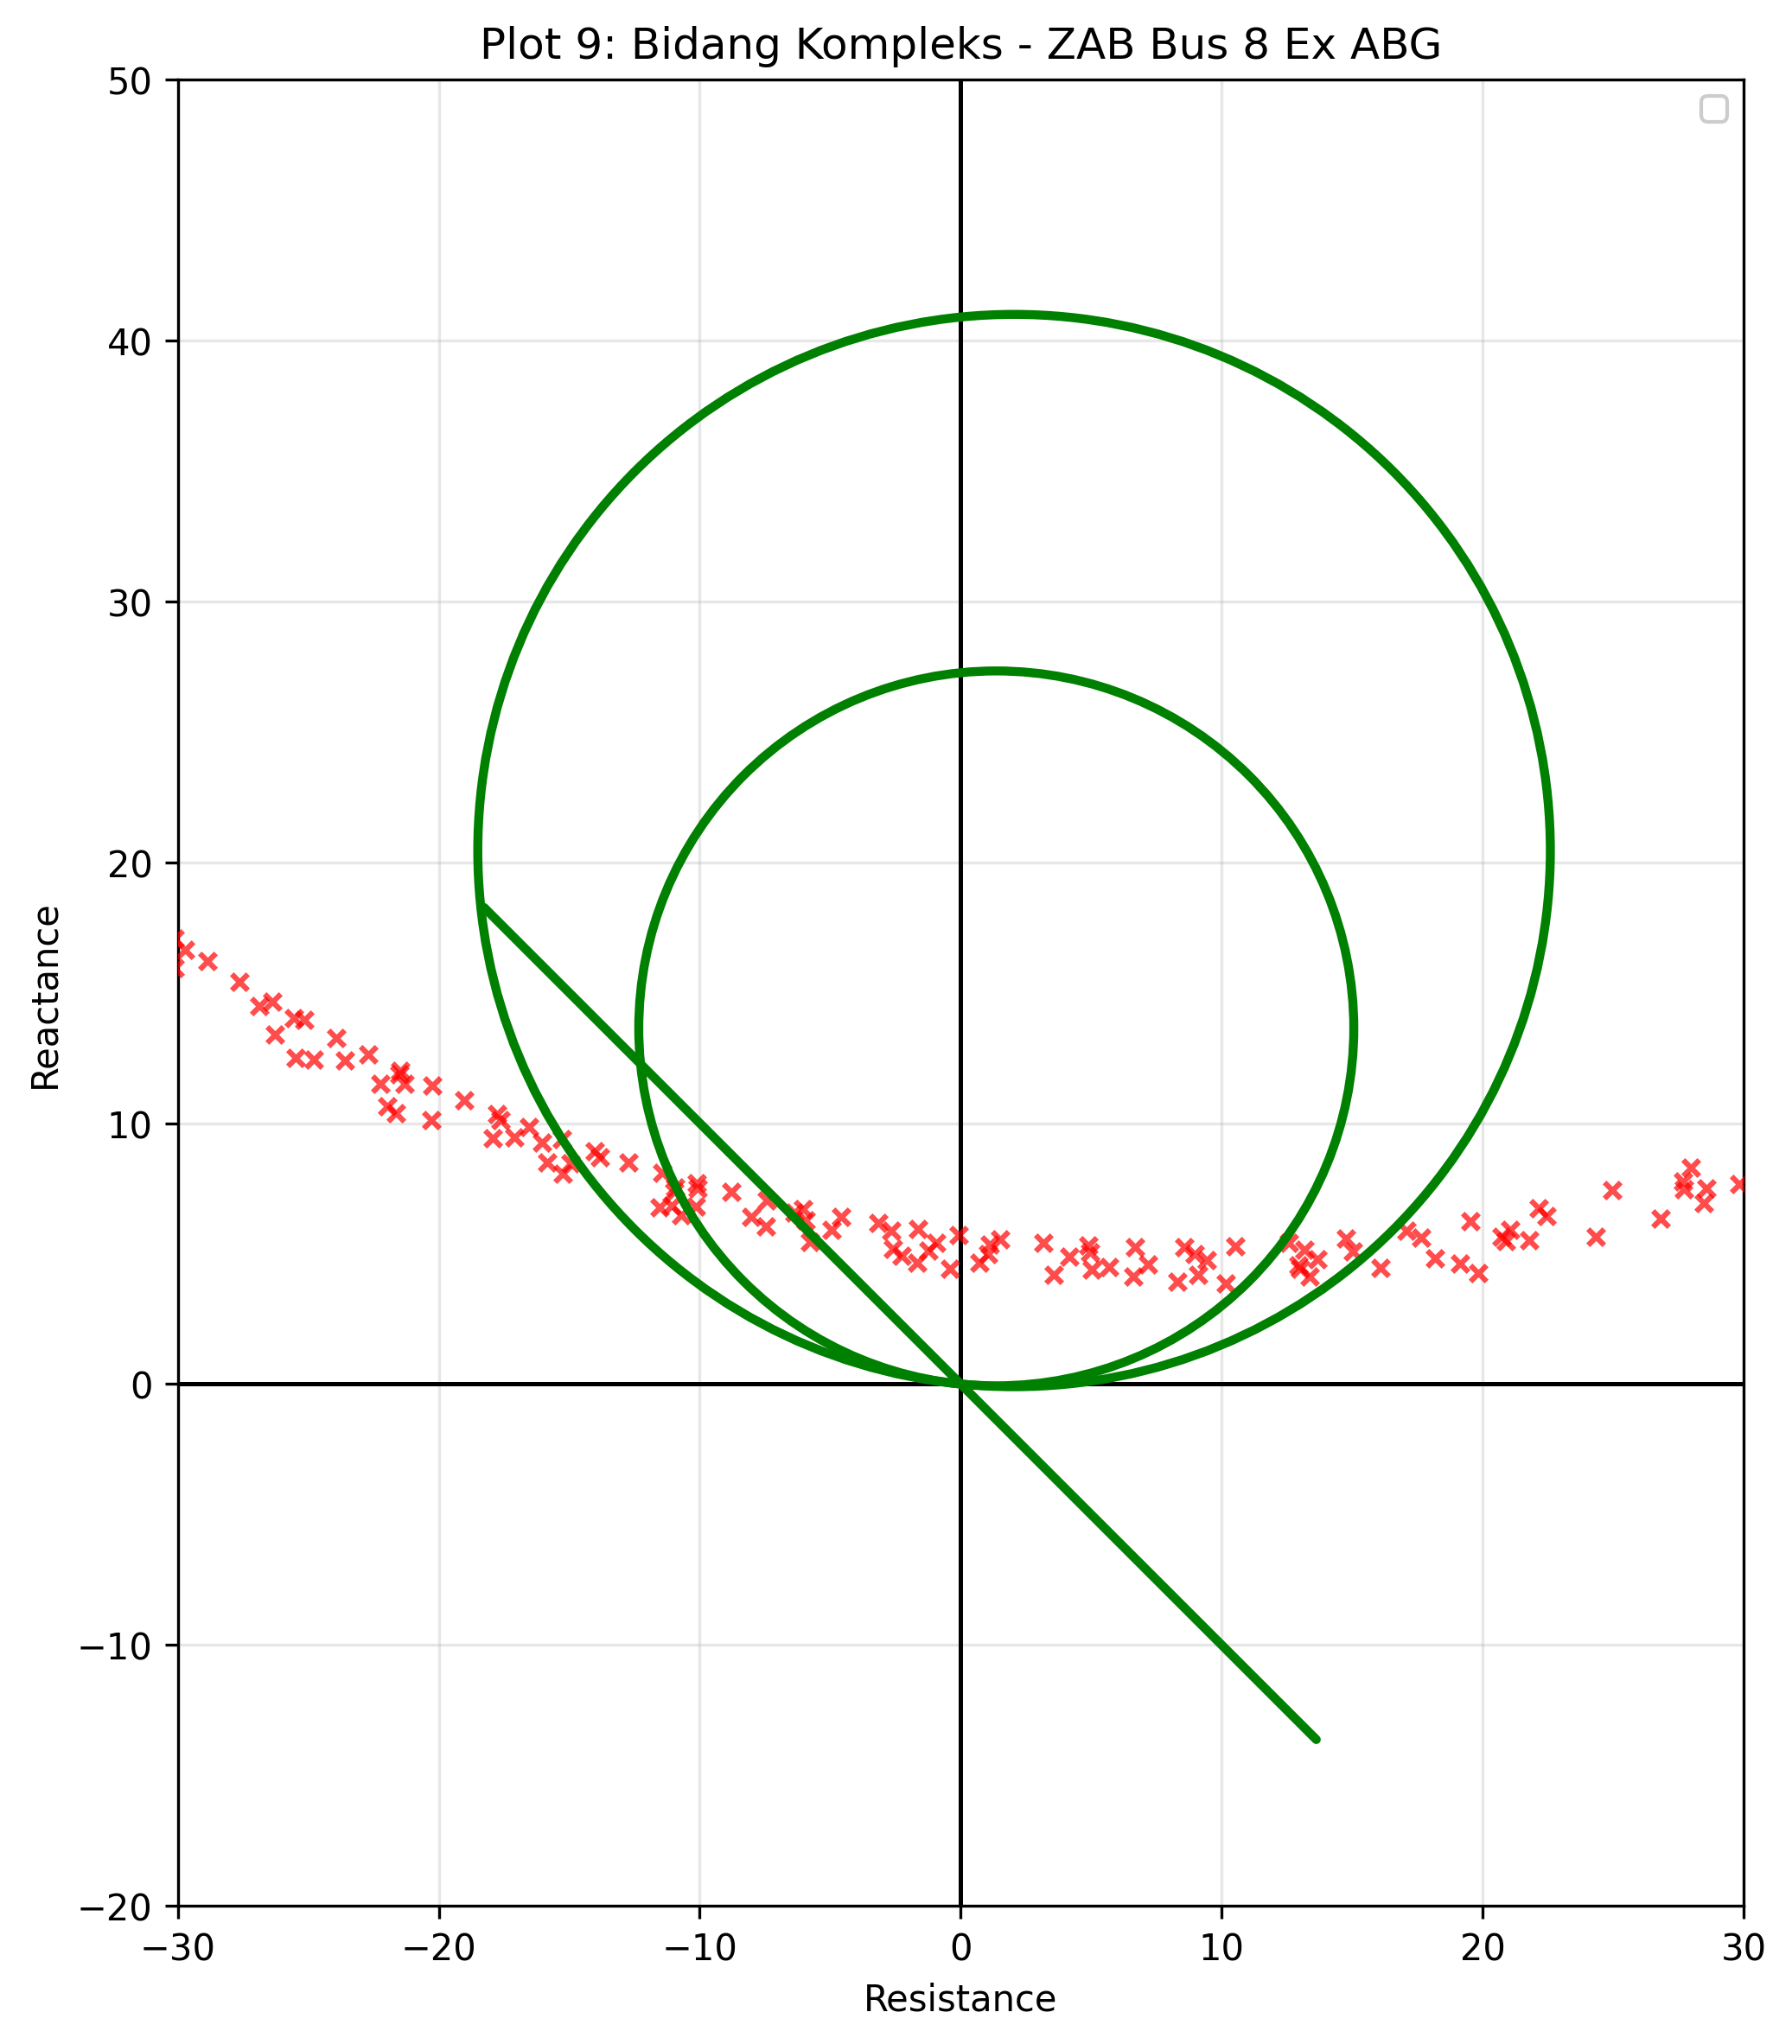
\includegraphics[width=0.8\textwidth]{contents/chapter-4/TIBR_09_ZAB_Bus_8_Ex_ABG.png}
    \caption{Impedansi Tampak ZAB Bus 8 External DLG Fault}
    \label{fig:TIBR_09_ZAB_Bus_8_Ex_ABG}
\end{figure}

Gambar \ref{fig:TIBR_09_ZAB_Bus_8_Ex_ABG} menunjukkan impedansi tampak loop fasa A dengan fasa B yang dibaca oleh relay 21 melalui CT dan VT pada Bus 8. Hasil plot memperlihatkan bahwa impedansi tampak masuk ke dalam zona 1 saat terjadi gangguan eksternal DLG. Relay memberikan perintah trip karena arus yang mengalir sudah membuat relay aktif dan melebihi batas arus maksimum untuk trip instan, sebagaimana ditunjukkan pada Gambar \ref{fig:Bus_8_Ex_DLG}.

\begin{figure}[H]
    \centering
    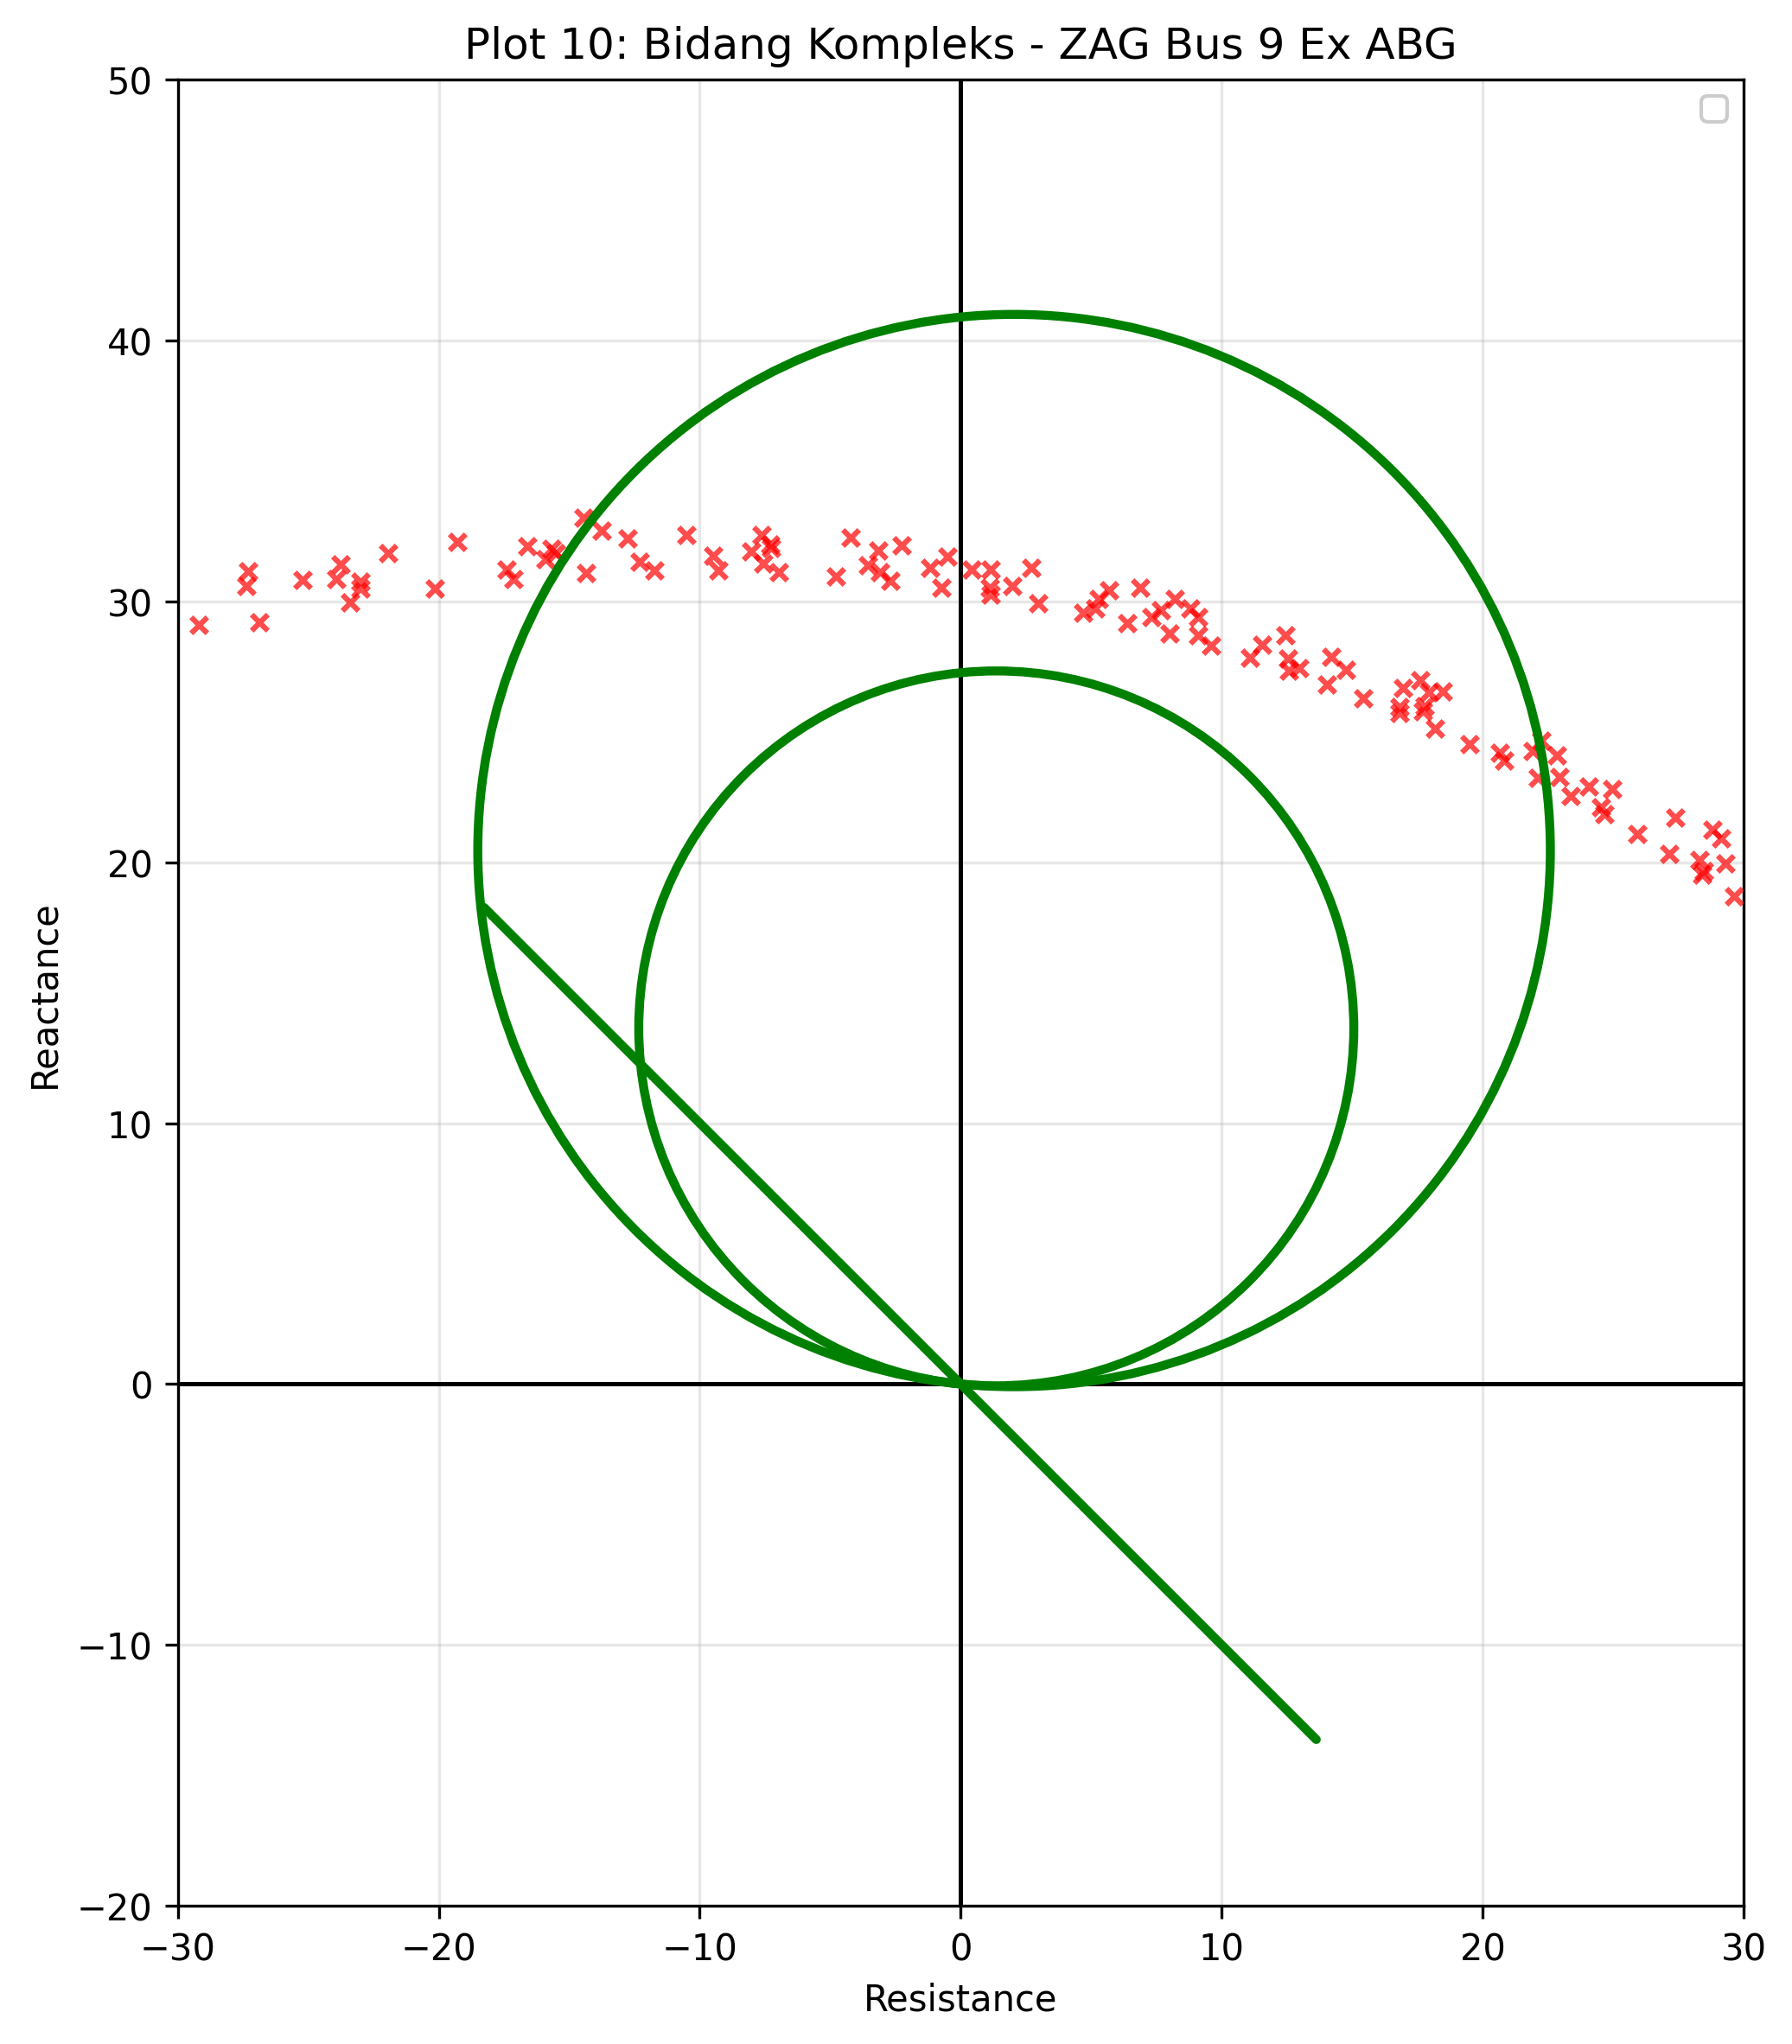
\includegraphics[width=0.8\textwidth]{contents/chapter-4/TIBR_10_ZAG_Bus_9_Ex_ABG.png}
    \caption{Impedansi Tampak ZAG Bus 9 External DLG Fault}
    \label{fig:TIBR_10_ZAG_Bus_9_Ex_ABG}
\end{figure}

Gambar \ref{fig:TIBR_10_ZAG_Bus_9_Ex_ABG} menunjukkan impedansi tampak loop fasa A dengan ground yang dibaca oleh relay 21 melalui CT dan VT pada Bus 9. Pada gangguan eksternal DLG, relay 21 sisi Bus 9 tidak membaca gangguan sebagai gangguan yang berada di arah depan relay. Oleh karena itu, relay tidak mengirimkan sinyal trip kepada CB dan responsnya tetap sesuai untuk gangguan eksternal.

\begin{figure}[H]
    \centering
    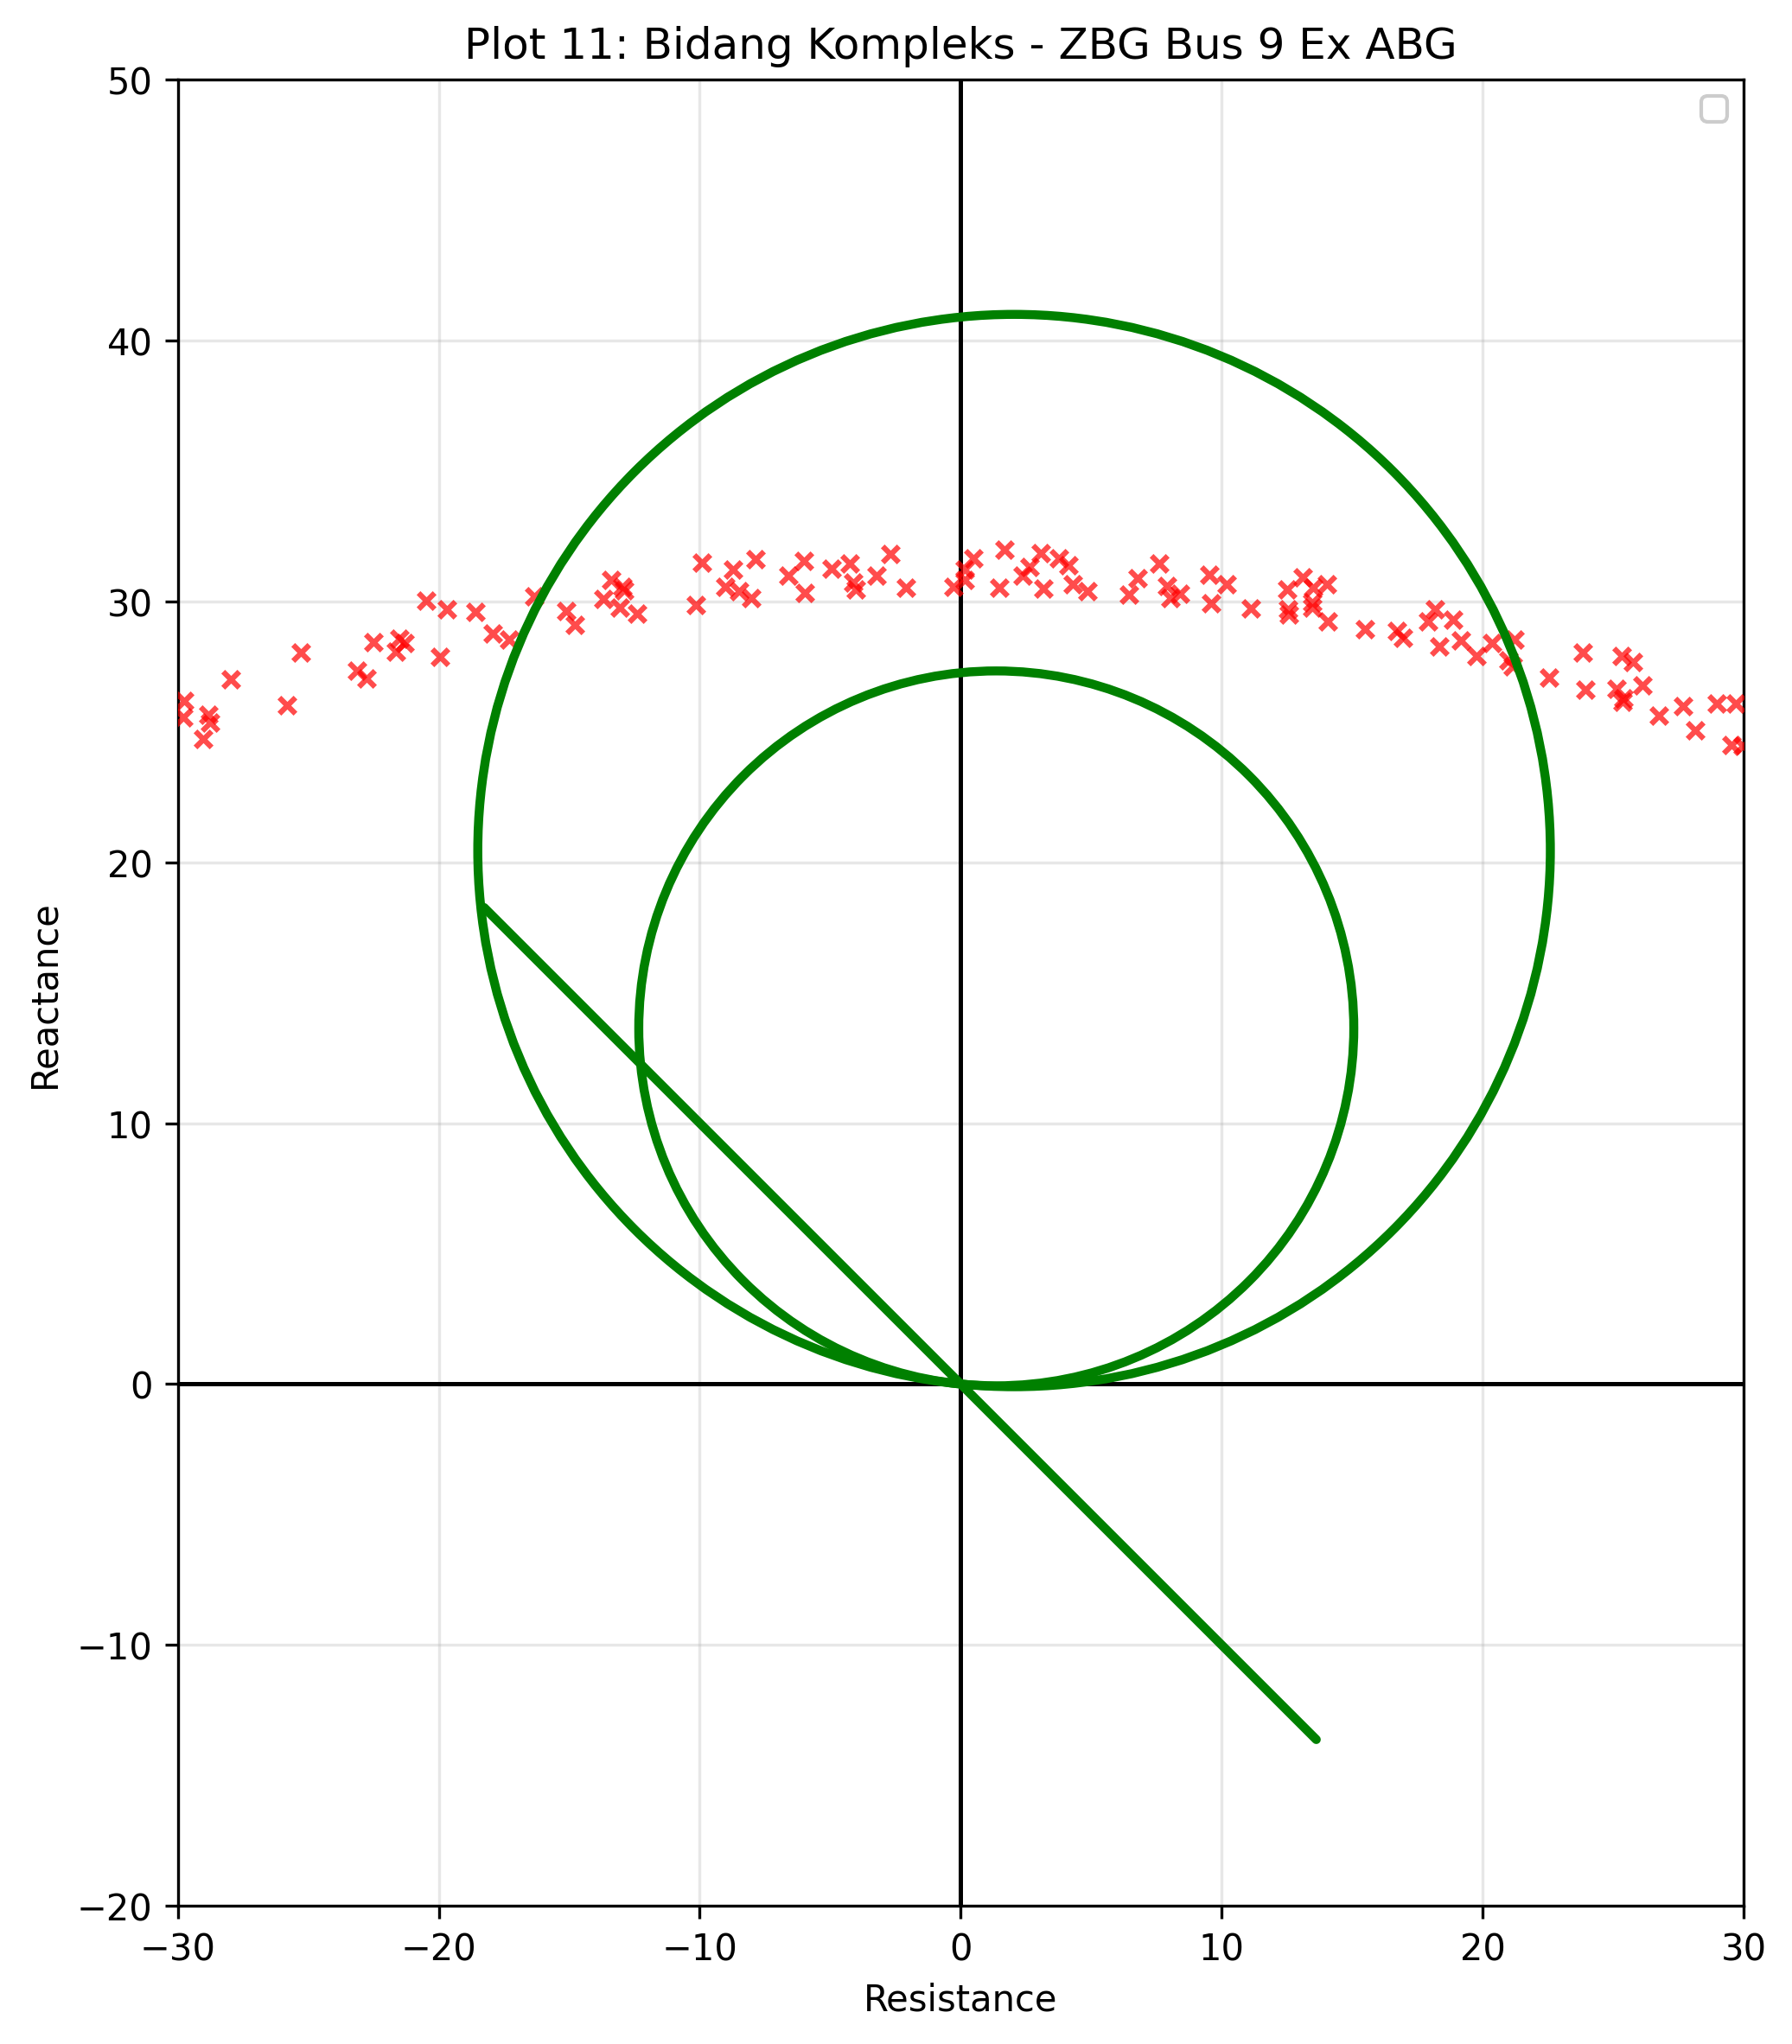
\includegraphics[width=0.8\textwidth]{contents/chapter-4/TIBR_11_ZBG_Bus_9_Ex_ABG.png}
    \caption{Impedansi Tampak ZBG Bus 9 External DLG Fault}
    \label{fig:TIBR_11_ZBG_Bus_9_Ex_ABG}
\end{figure}

Gambar \ref{fig:TIBR_11_ZBG_Bus_9_Ex_ABG} menunjukkan impedansi tampak loop fasa B dengan ground yang dibaca oleh relay 21 melalui CT dan VT pada Bus 9. Hasil plot menunjukkan bahwa relay tidak mendeteksi gangguan eksternal DLG sebagai gangguan di depan relay. Dengan pembacaan tersebut, relay 21 sisi Bus 9 tidak mengirimkan sinyal trip kepada CB.

\begin{figure}[H]
    \centering
    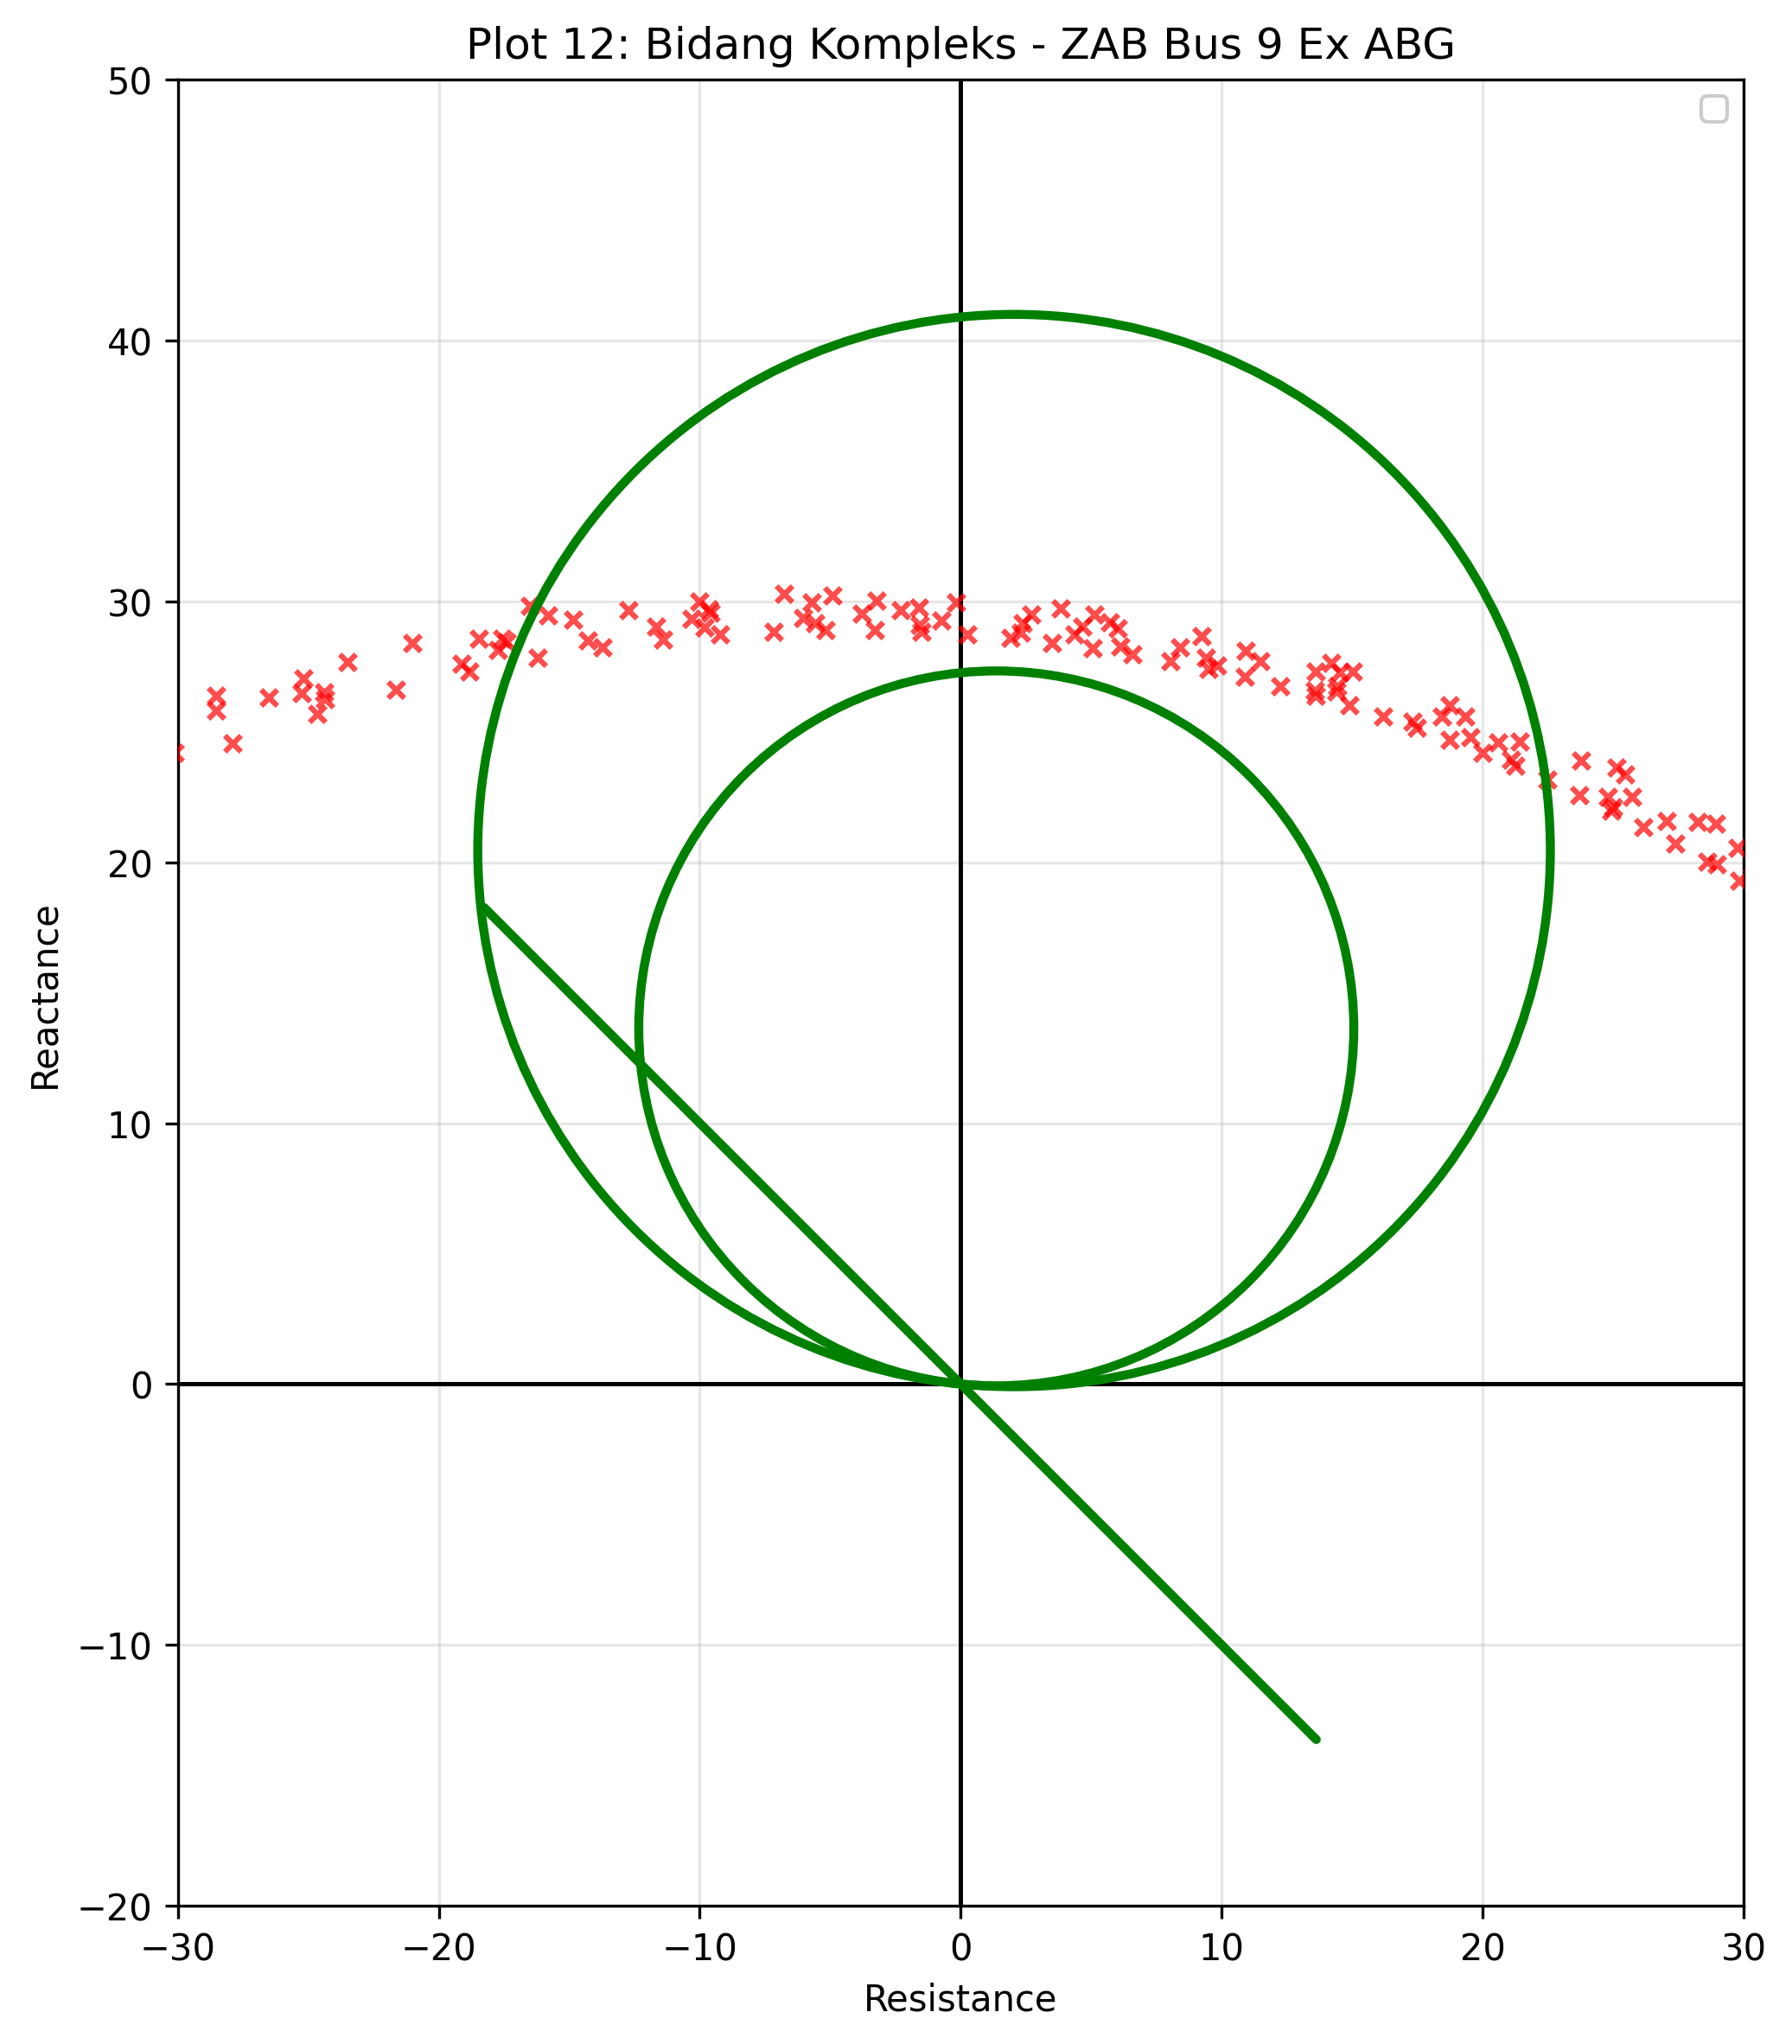
\includegraphics[width=0.8\textwidth]{contents/chapter-4/TIBR_12_ZAB_Bus_9_Ex_ABG.png}
    \caption{Impedansi Tampak ZAB Bus 9 External DLG Fault}
    \label{fig:TIBR_12_ZAB_Bus_9_Ex_ABG}
\end{figure}

Gambar \ref{fig:TIBR_12_ZAB_Bus_9_Ex_ABG} menunjukkan impedansi tampak loop fasa A dengan fasa B yang dibaca oleh relay 21 melalui CT dan VT pada Bus 9. Pada gangguan eksternal DLG, relay tidak membaca gangguan berada pada arah depan relay. Akibatnya, relay 21 sisi Bus 9 tidak mengirimkan sinyal trip kepada CB, sehingga respons pada elemen ini konsisten dengan pembacaan elemen lainnya di sisi Bus 9.

\begin{figure}[H]
    \centering
    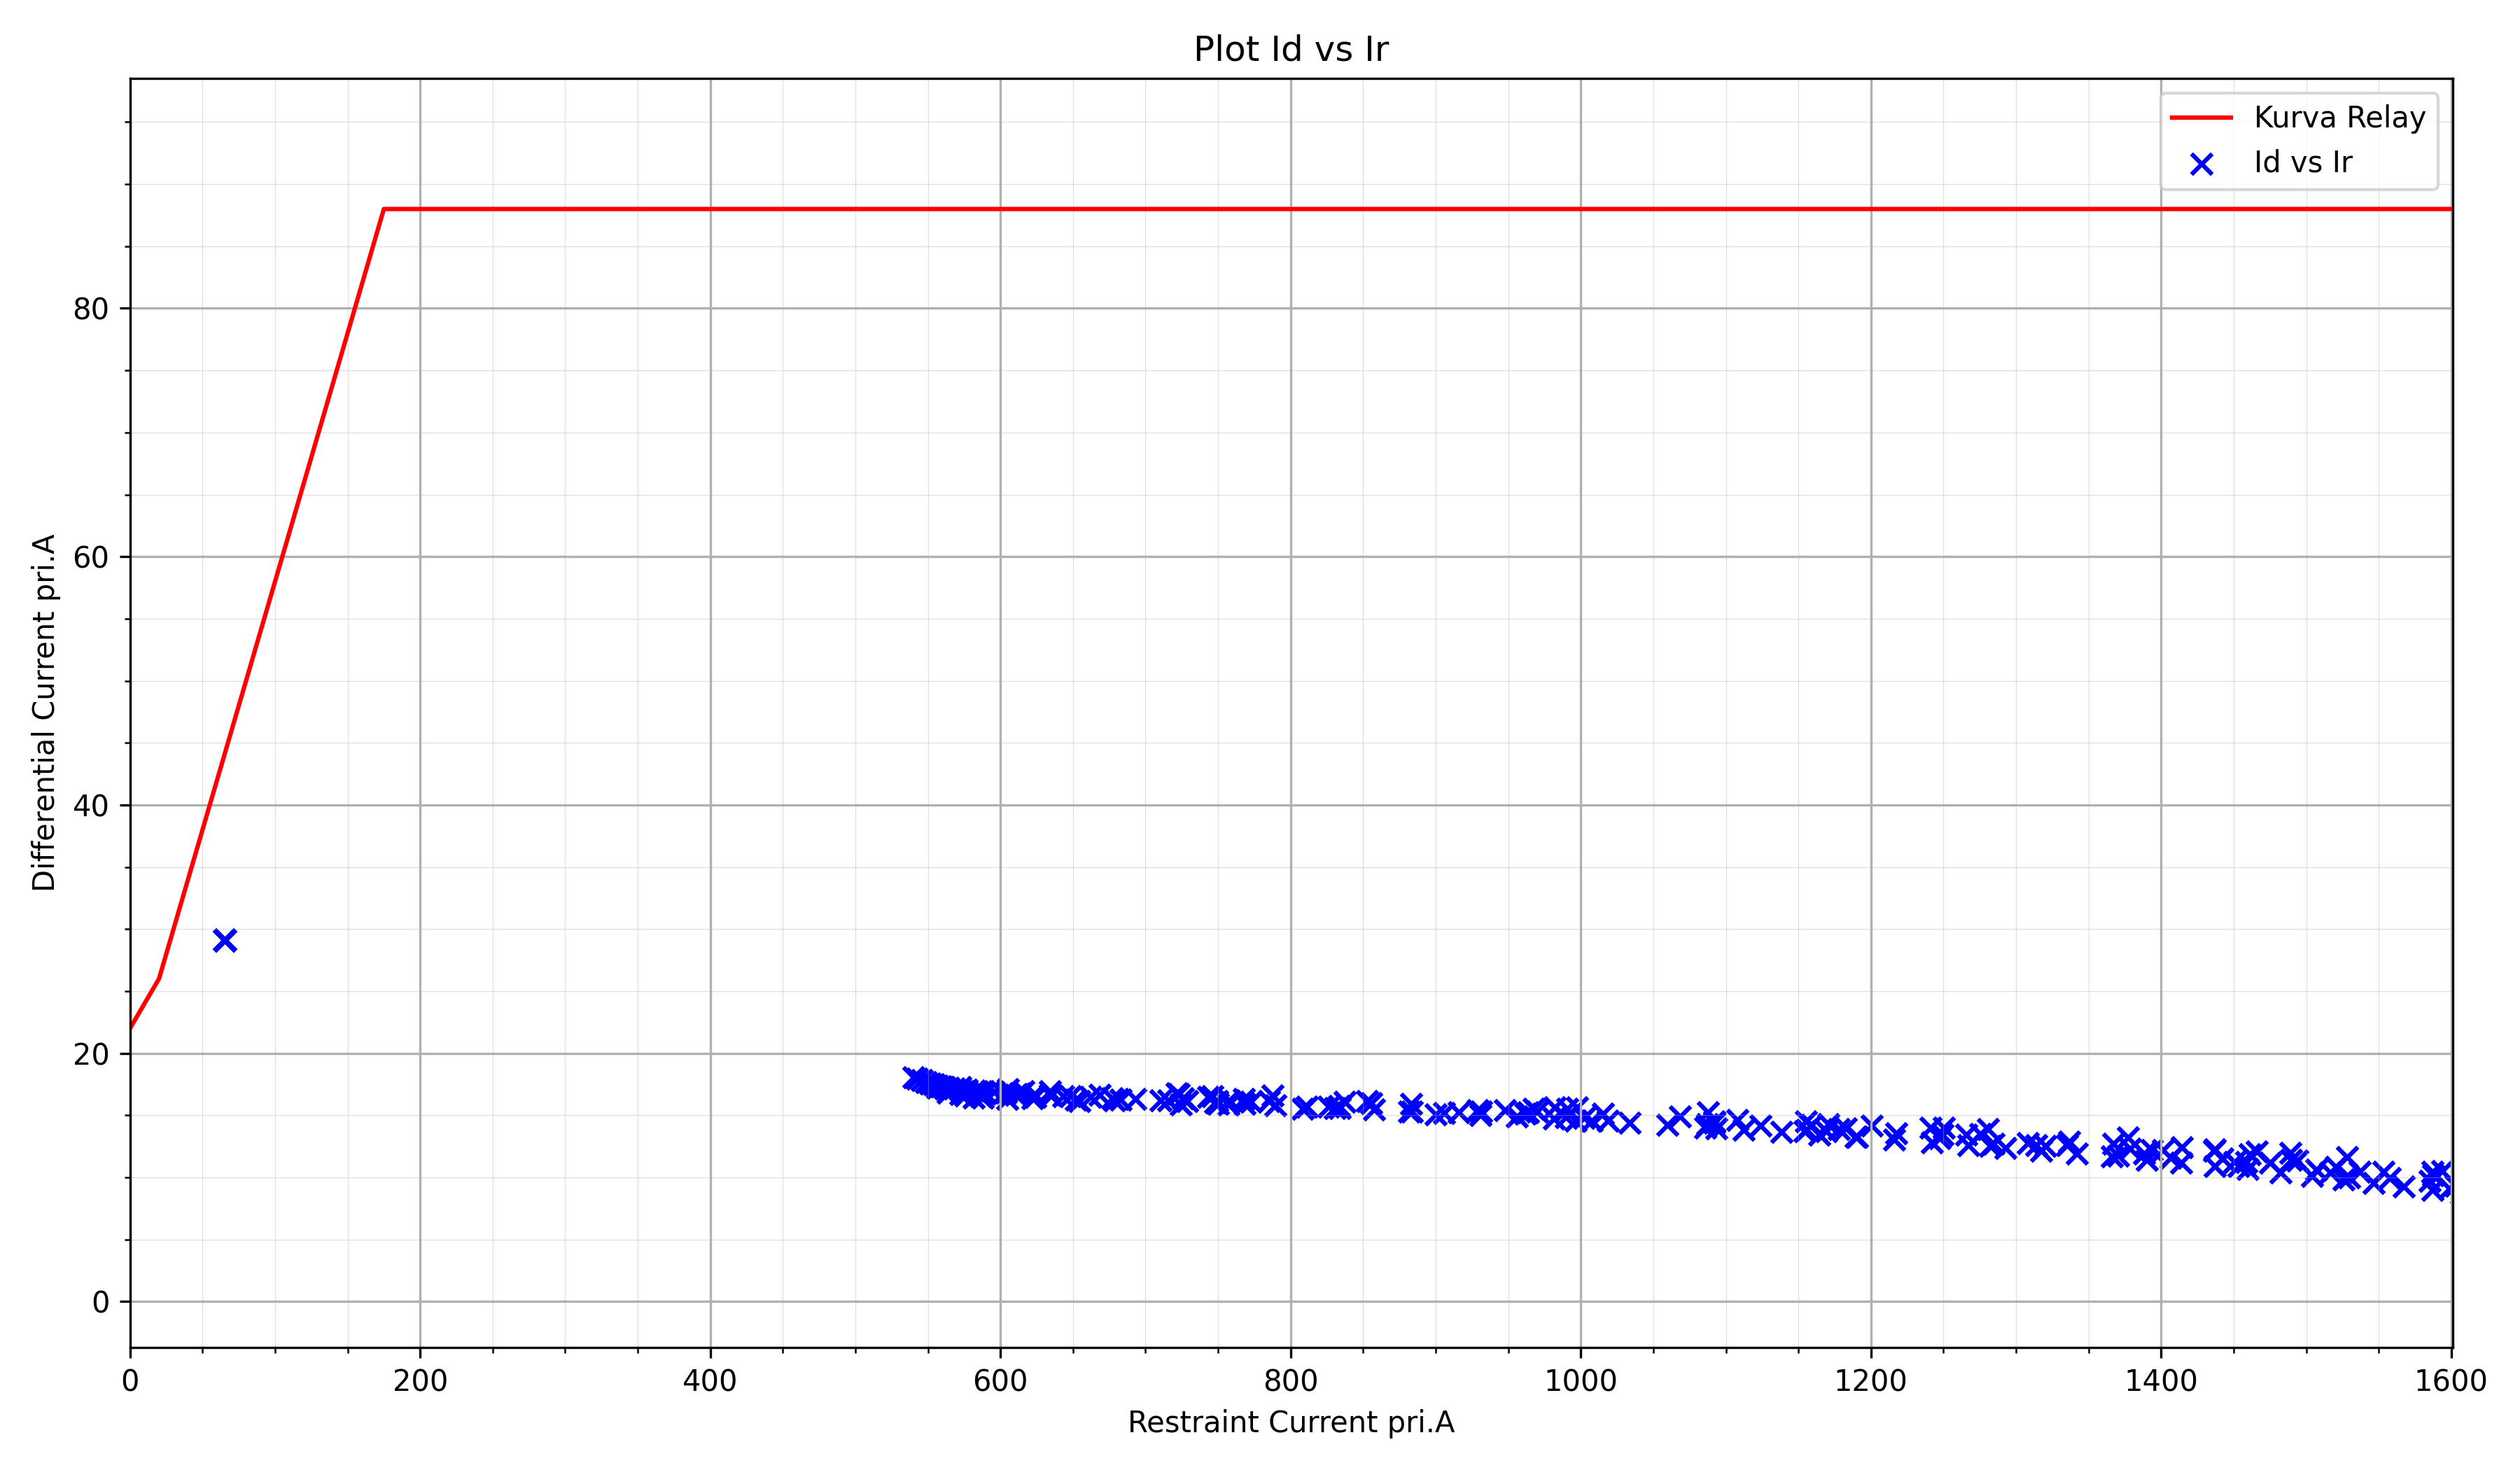
\includegraphics[width=0.8\textwidth]{contents/chapter-4/87LTIBR_plot_Ax2_Ay2.png}
    \caption{Current Comparison Differential Fasa A External DLG Fault}
    \label{fig:87LTIBR_plot_Ax2_Ay2}
\end{figure}

Gambar \ref{fig:87LTIBR_plot_Ax2_Ay2} menunjukkan plot \textit{current comparison differential} pada fasa A saat terjadi gangguan eksternal DLG. Titik arus berada di bawah batas operasi yang ditentukan oleh setting relay. Kondisi ini menunjukkan bahwa relay 87L tidak membaca gangguan sebagai gangguan internal dan tidak memerintahkan trip pada CB.

\begin{figure}[H]
    \centering
    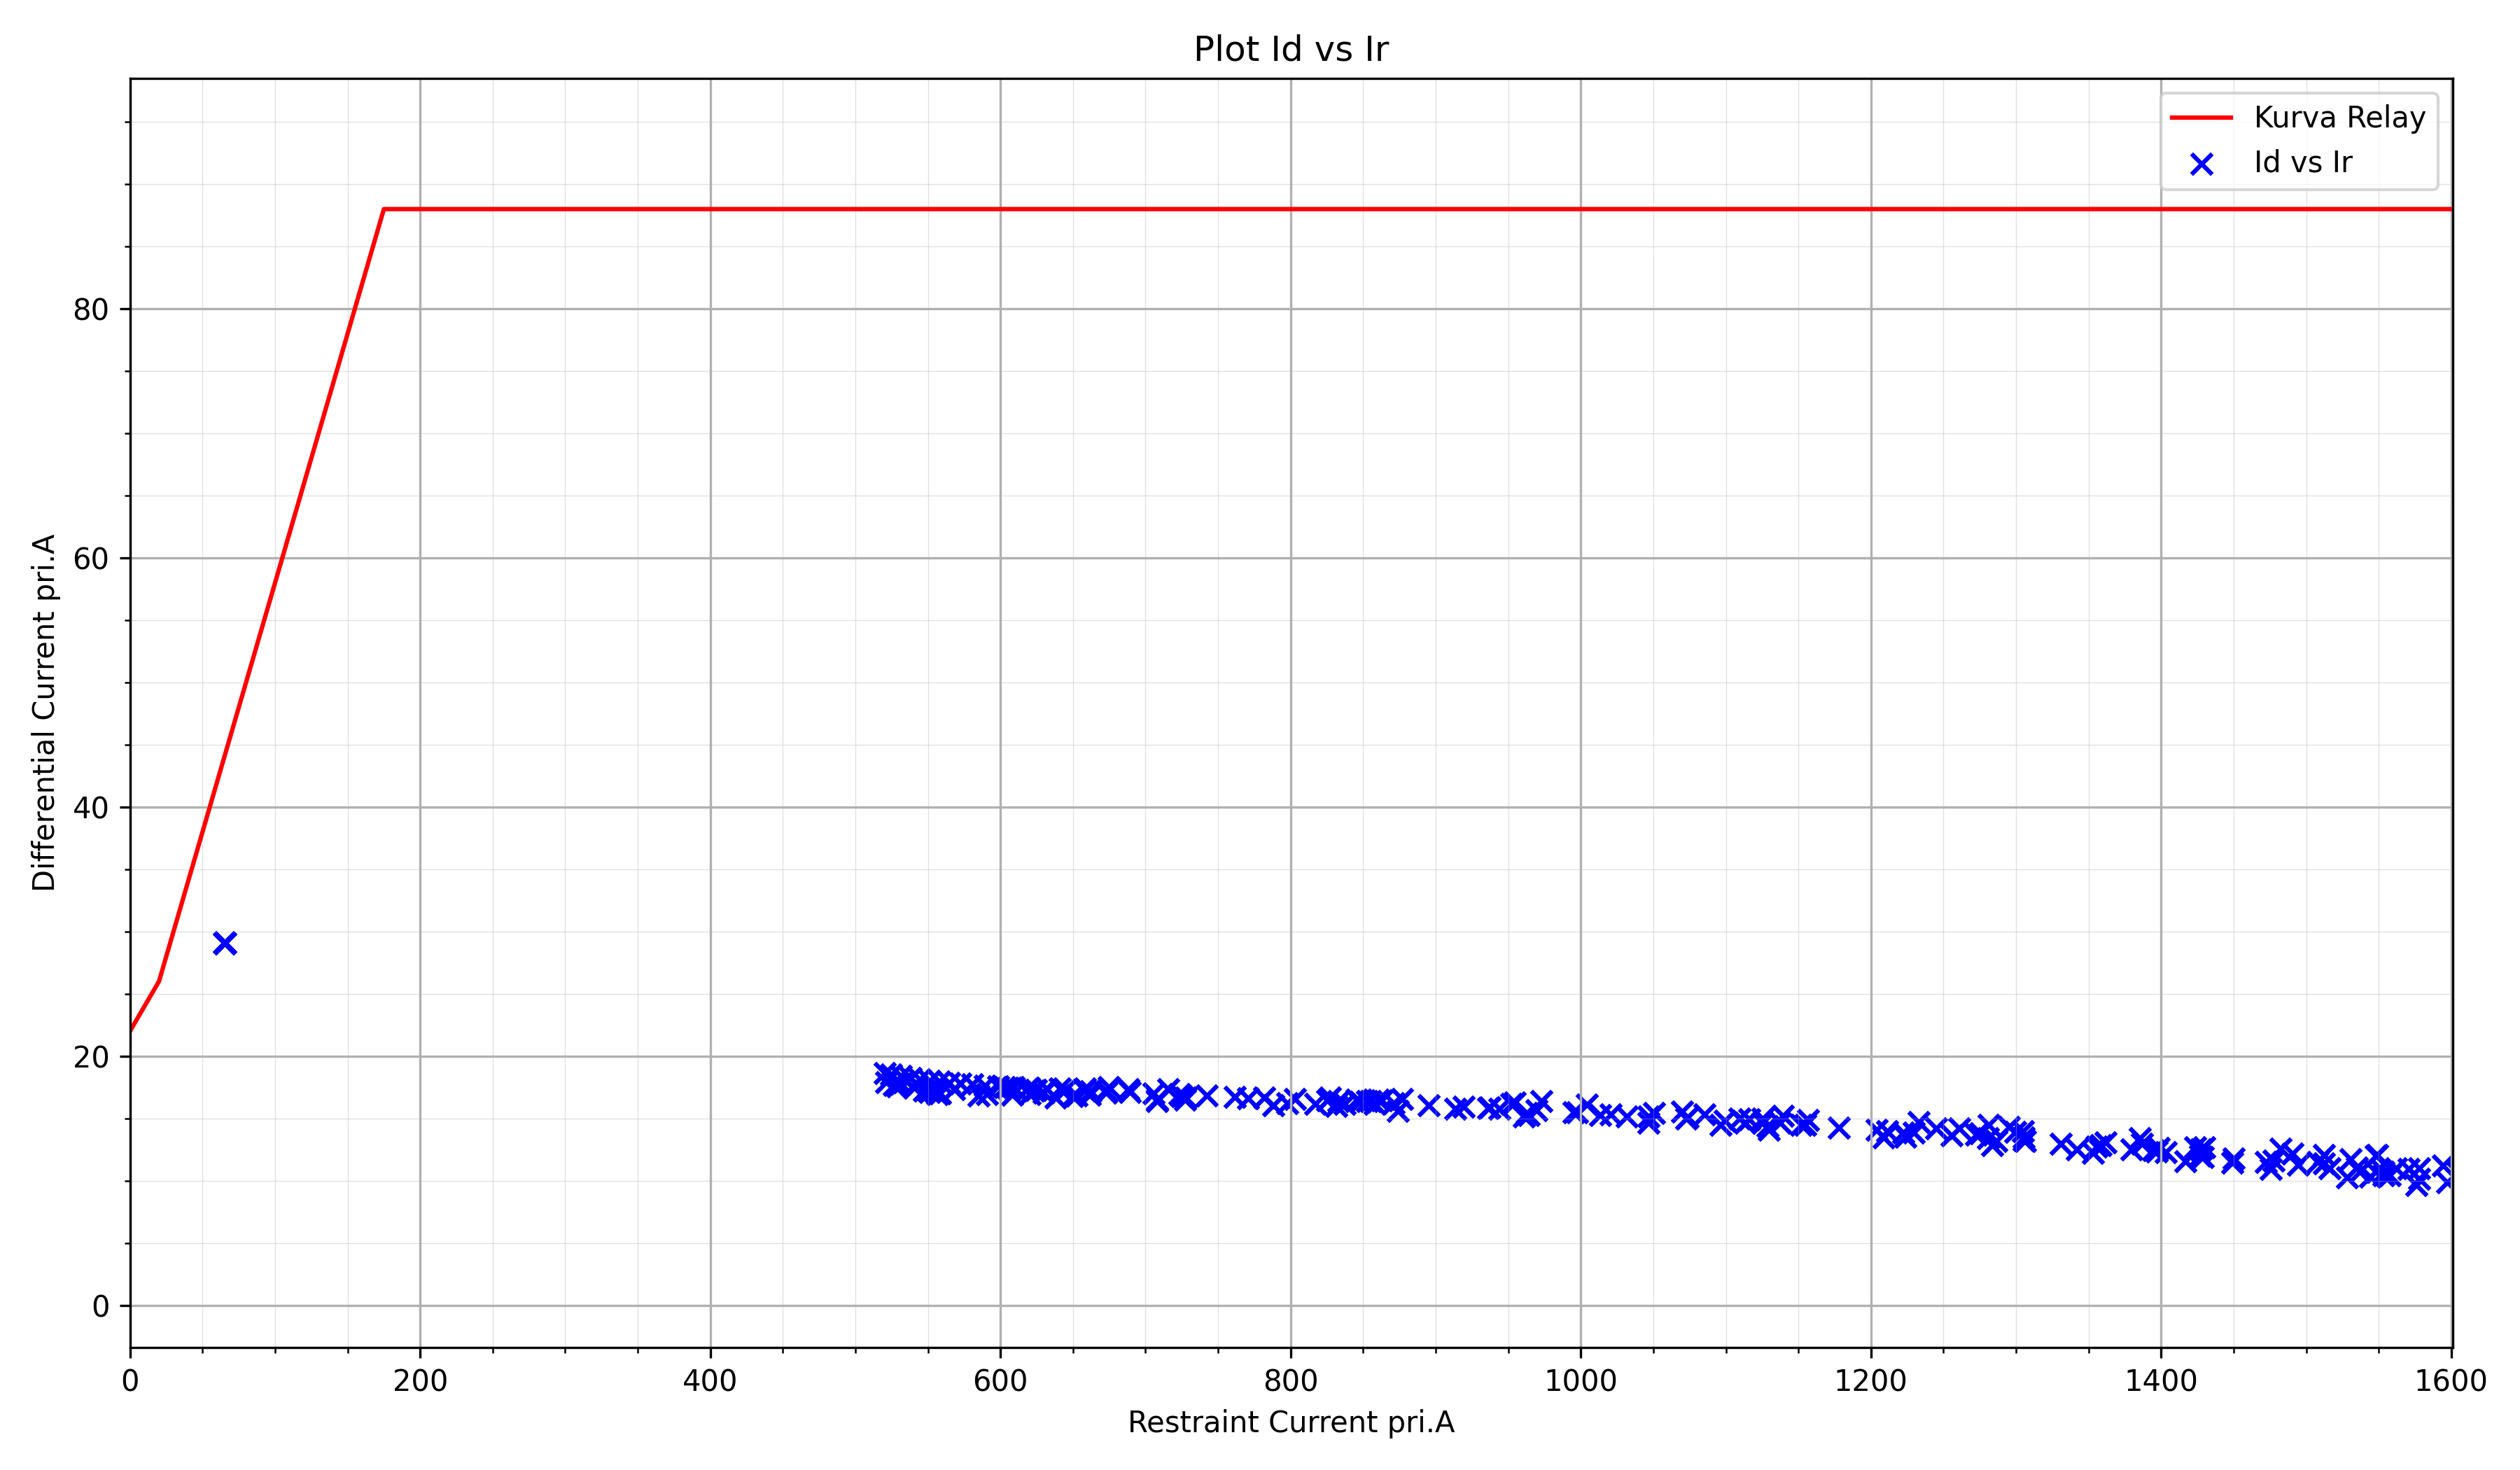
\includegraphics[width=0.8\textwidth]{contents/chapter-4/87LTIBR_plot_Bx2_By2.png}
    \caption{Current Comparison Differential Fasa B External DLG Fault}
    \label{fig:87LTIBR_plot_Bx2_By2}
\end{figure}

Gambar \ref{fig:87LTIBR_plot_Bx2_By2} menunjukkan plot \textit{current comparison differential} pada fasa B saat terjadi gangguan eksternal DLG. Pada plot tersebut, titik arus masih berada di bawah batas operasi relay. Dengan demikian, relay 87L tetap berada pada daerah penahan dan tidak mengeluarkan perintah trip kepada CB.

\begin{figure}[H]
    \centering
    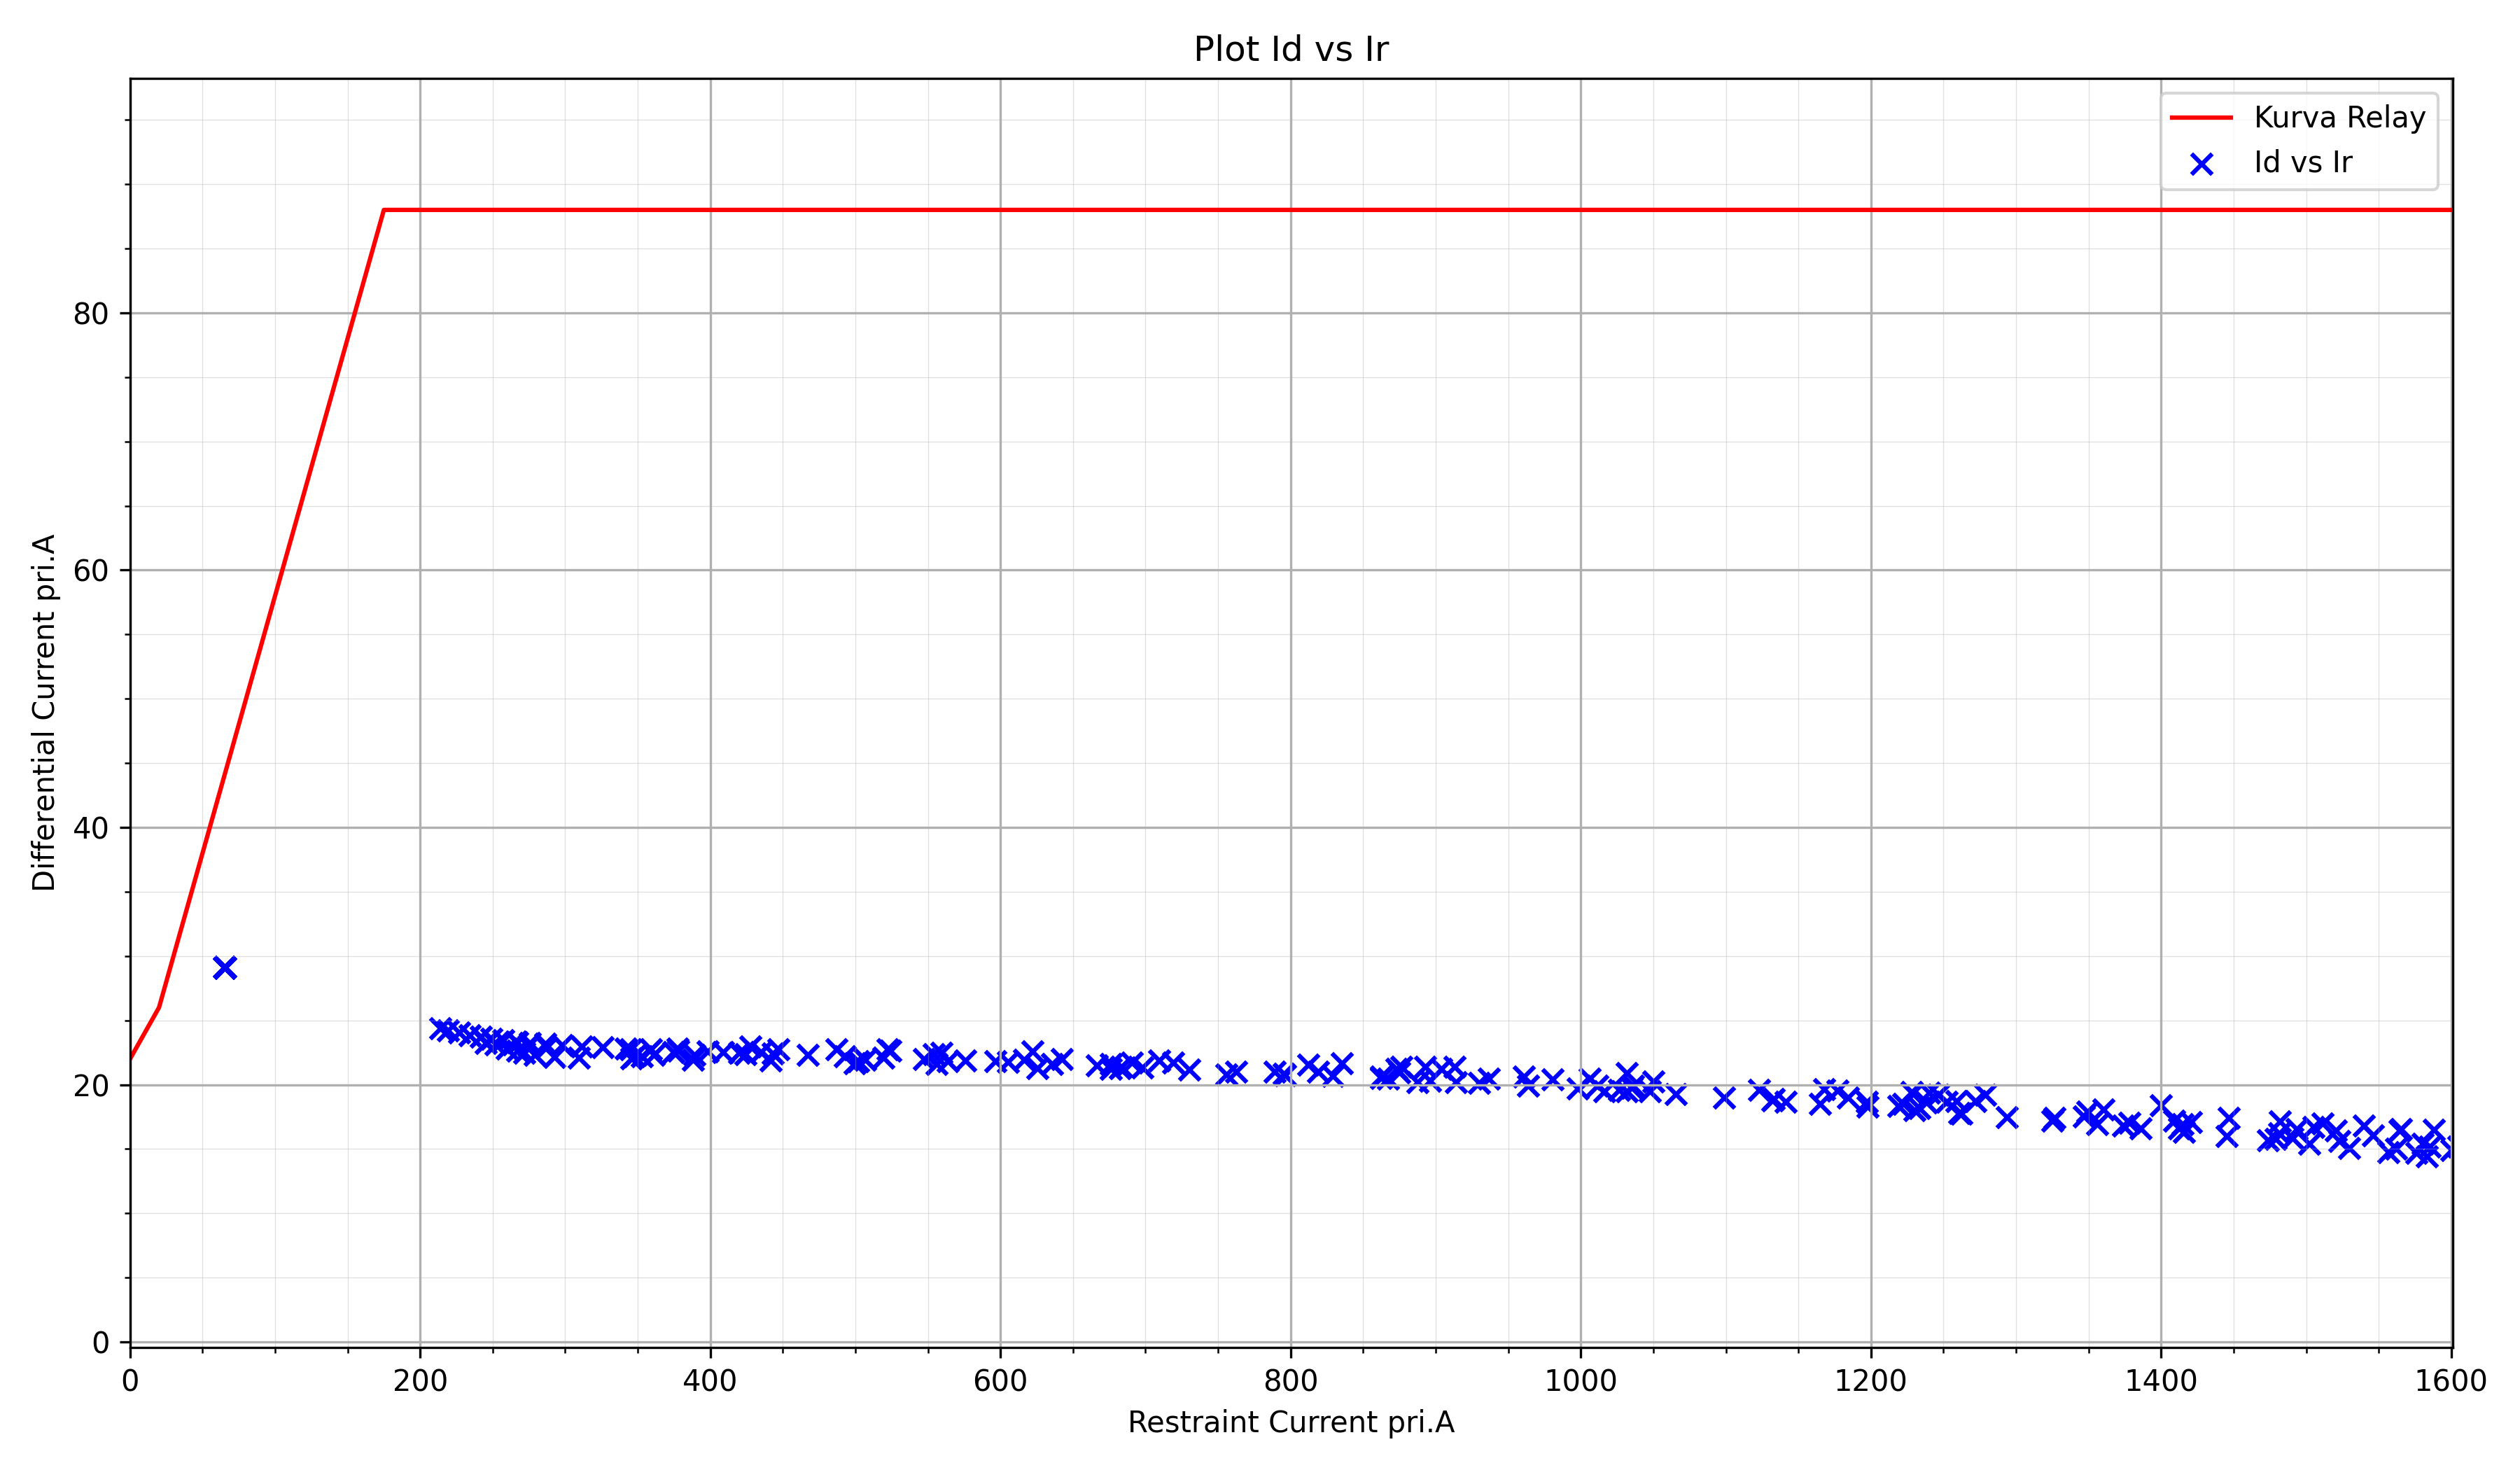
\includegraphics[width=0.8\textwidth]{contents/chapter-4/87LTIBR_plot_Cx2_Cy2.png}
    \caption{Current Comparison Differential Fasa C External DLG Fault}
    \label{fig:87LTIBR_plot_Cx2_Cy2}
\end{figure}

Gambar \ref{fig:87LTIBR_plot_Cx2_Cy2} menunjukkan plot \textit{current comparison differential} pada fasa C saat terjadi gangguan eksternal DLG. Titik arus pada fasa C berada di bawah batas operasi yang ditentukan oleh setting relay. Oleh karena itu, relay 87L membaca kondisi tersebut sebagai gangguan di luar daerah proteksi dan tidak memerintahkan trip pada CB.

\section{Perbandingan Kontribusi Arus Hubung Singkat antar Jenis IBR}

Subbab ini membahas perbandingan kontribusi hubung singkat dari masing-masing jenis IBR yang digunakan pada skenario penelitian, yaitu \textit{wind turbine type 3}, \textit{wind turbine type 4}, dan \textit{photovoltaic}. Pembahasan ini ditempatkan sebelum analisis respons relay karena besar kecilnya kontribusi arus gangguan dari sumber IBR dapat memengaruhi besaran listrik yang dibaca oleh relay, terutama pada kondisi gangguan dan konfigurasi jaringan tertentu.

Model IBR yang digunakan pada penelitian ini merupakan model yang tersedia pada DIgSILENT PowerFactory, yaitu model WECC untuk \textit{wind turbine type 3} dan \textit{wind turbine type 4}, serta model \textit{distributed small PV plants} untuk \textit{photovoltaic}. Model tersebut digunakan tanpa modifikasi terhadap struktur maupun karakteristik internalnya karena pembahasan penelitian ini tidak diarahkan untuk mengevaluasi model dinamik atau kontrol internal IBR. Fokus penelitian ditempatkan pada pengaruh keberadaan masing-masing jenis IBR terhadap kontribusi arus hubung singkat dan respons relay proteksi saluran.

Hasil kontribusi hubung singkat pada bagian ini digunakan sebagai konteks awal untuk membaca perubahan respons relay 21 dan relay 87L pada subbab berikutnya. Dengan membandingkan kontribusi setiap jenis IBR, pengaruh karakteristik sumber terhadap arus gangguan dapat ditelusuri lebih jelas sebelum dikaitkan dengan impedansi tampak, syarat \textit{starting}, arus diferensial, arus \textit{restraint}, dan keputusan operasi relay.

\subsection{Wind Turbine Type 3}

Pembahasan pada model \textit{wind turbine type 3} diawali dari pengaturan hubung singkat yang digunakan pada simulasi. Pengaturan ini penting karena WT Type 3 memiliki karakteristik yang berbeda dari WT Type 4. WT Type 3 masih menggunakan generator induksi \textit{doubly fed}, tetapi kontribusi arus gangguannya pada simulasi tetap bergantung pada parameter hubung singkat yang dimasukkan pada model.

\begin{figure}[H]
    \centering
    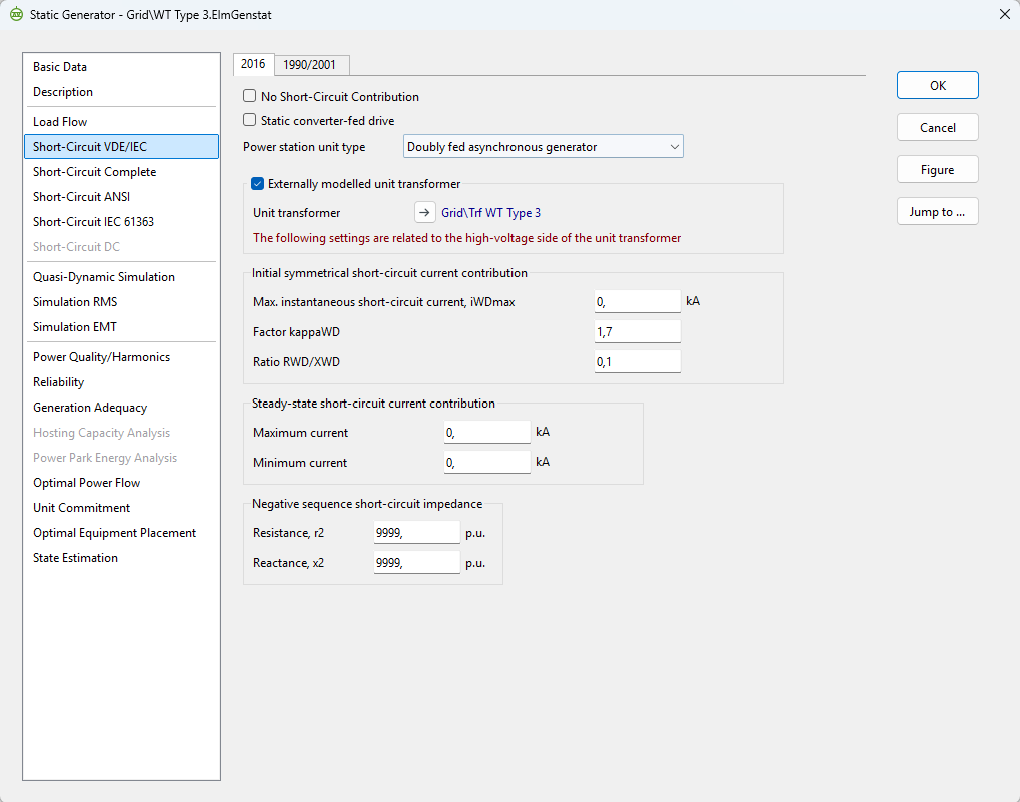
\includegraphics[width=0.8\textwidth]{contents/chapter-4/SC_Setting_WTT3.png}
    \caption{Setting Short Circuit Pada Model Wind Turbine Type 3}
    \label{fig:SC_Setting_WTT3}
\end{figure}

Gambar \ref{fig:SC_Setting_WTT3} menunjukkan bahwa model WT Type 3 pada tab VDE/IEC untuk hubung singkat menggunakan tipe unit \textit{doubly fed asynchronous generator} dengan transformator unit yang dimodelkan secara eksternal. Pada pengaturan tersebut, opsi \textit{No Short-Circuit Contribution} tidak diaktifkan. Namun, nilai kontribusi arus hubung singkat yang dimasukkan pada model bernilai 0 $\mathrm{kA}$, sehingga model tidak memberikan kontribusi arus gangguan pada kondisi yang dihitung.

Parameter pada Gambar \ref{fig:SC_Setting_WTT3} memperlihatkan bahwa nilai \textit{max. instantaneous short-circuit current} ditetapkan sebesar 0 $\mathrm{kA}$. Pada bagian \textit{steady-state short-circuit current contribution}, arus maksimum dan arus minimum juga bernilai 0 $\mathrm{kA}$. Selain itu, impedansi urutan negatif pada parameter $r_2$ dan $x_2$ ditetapkan sangat besar, yaitu 9999 p.u. Kombinasi pengaturan ini menunjukkan bahwa WT Type 3 tidak menyediakan jalur kontribusi arus gangguan yang signifikan pada simulasi hubung singkat.

\begin{figure}[H]
    \centering
    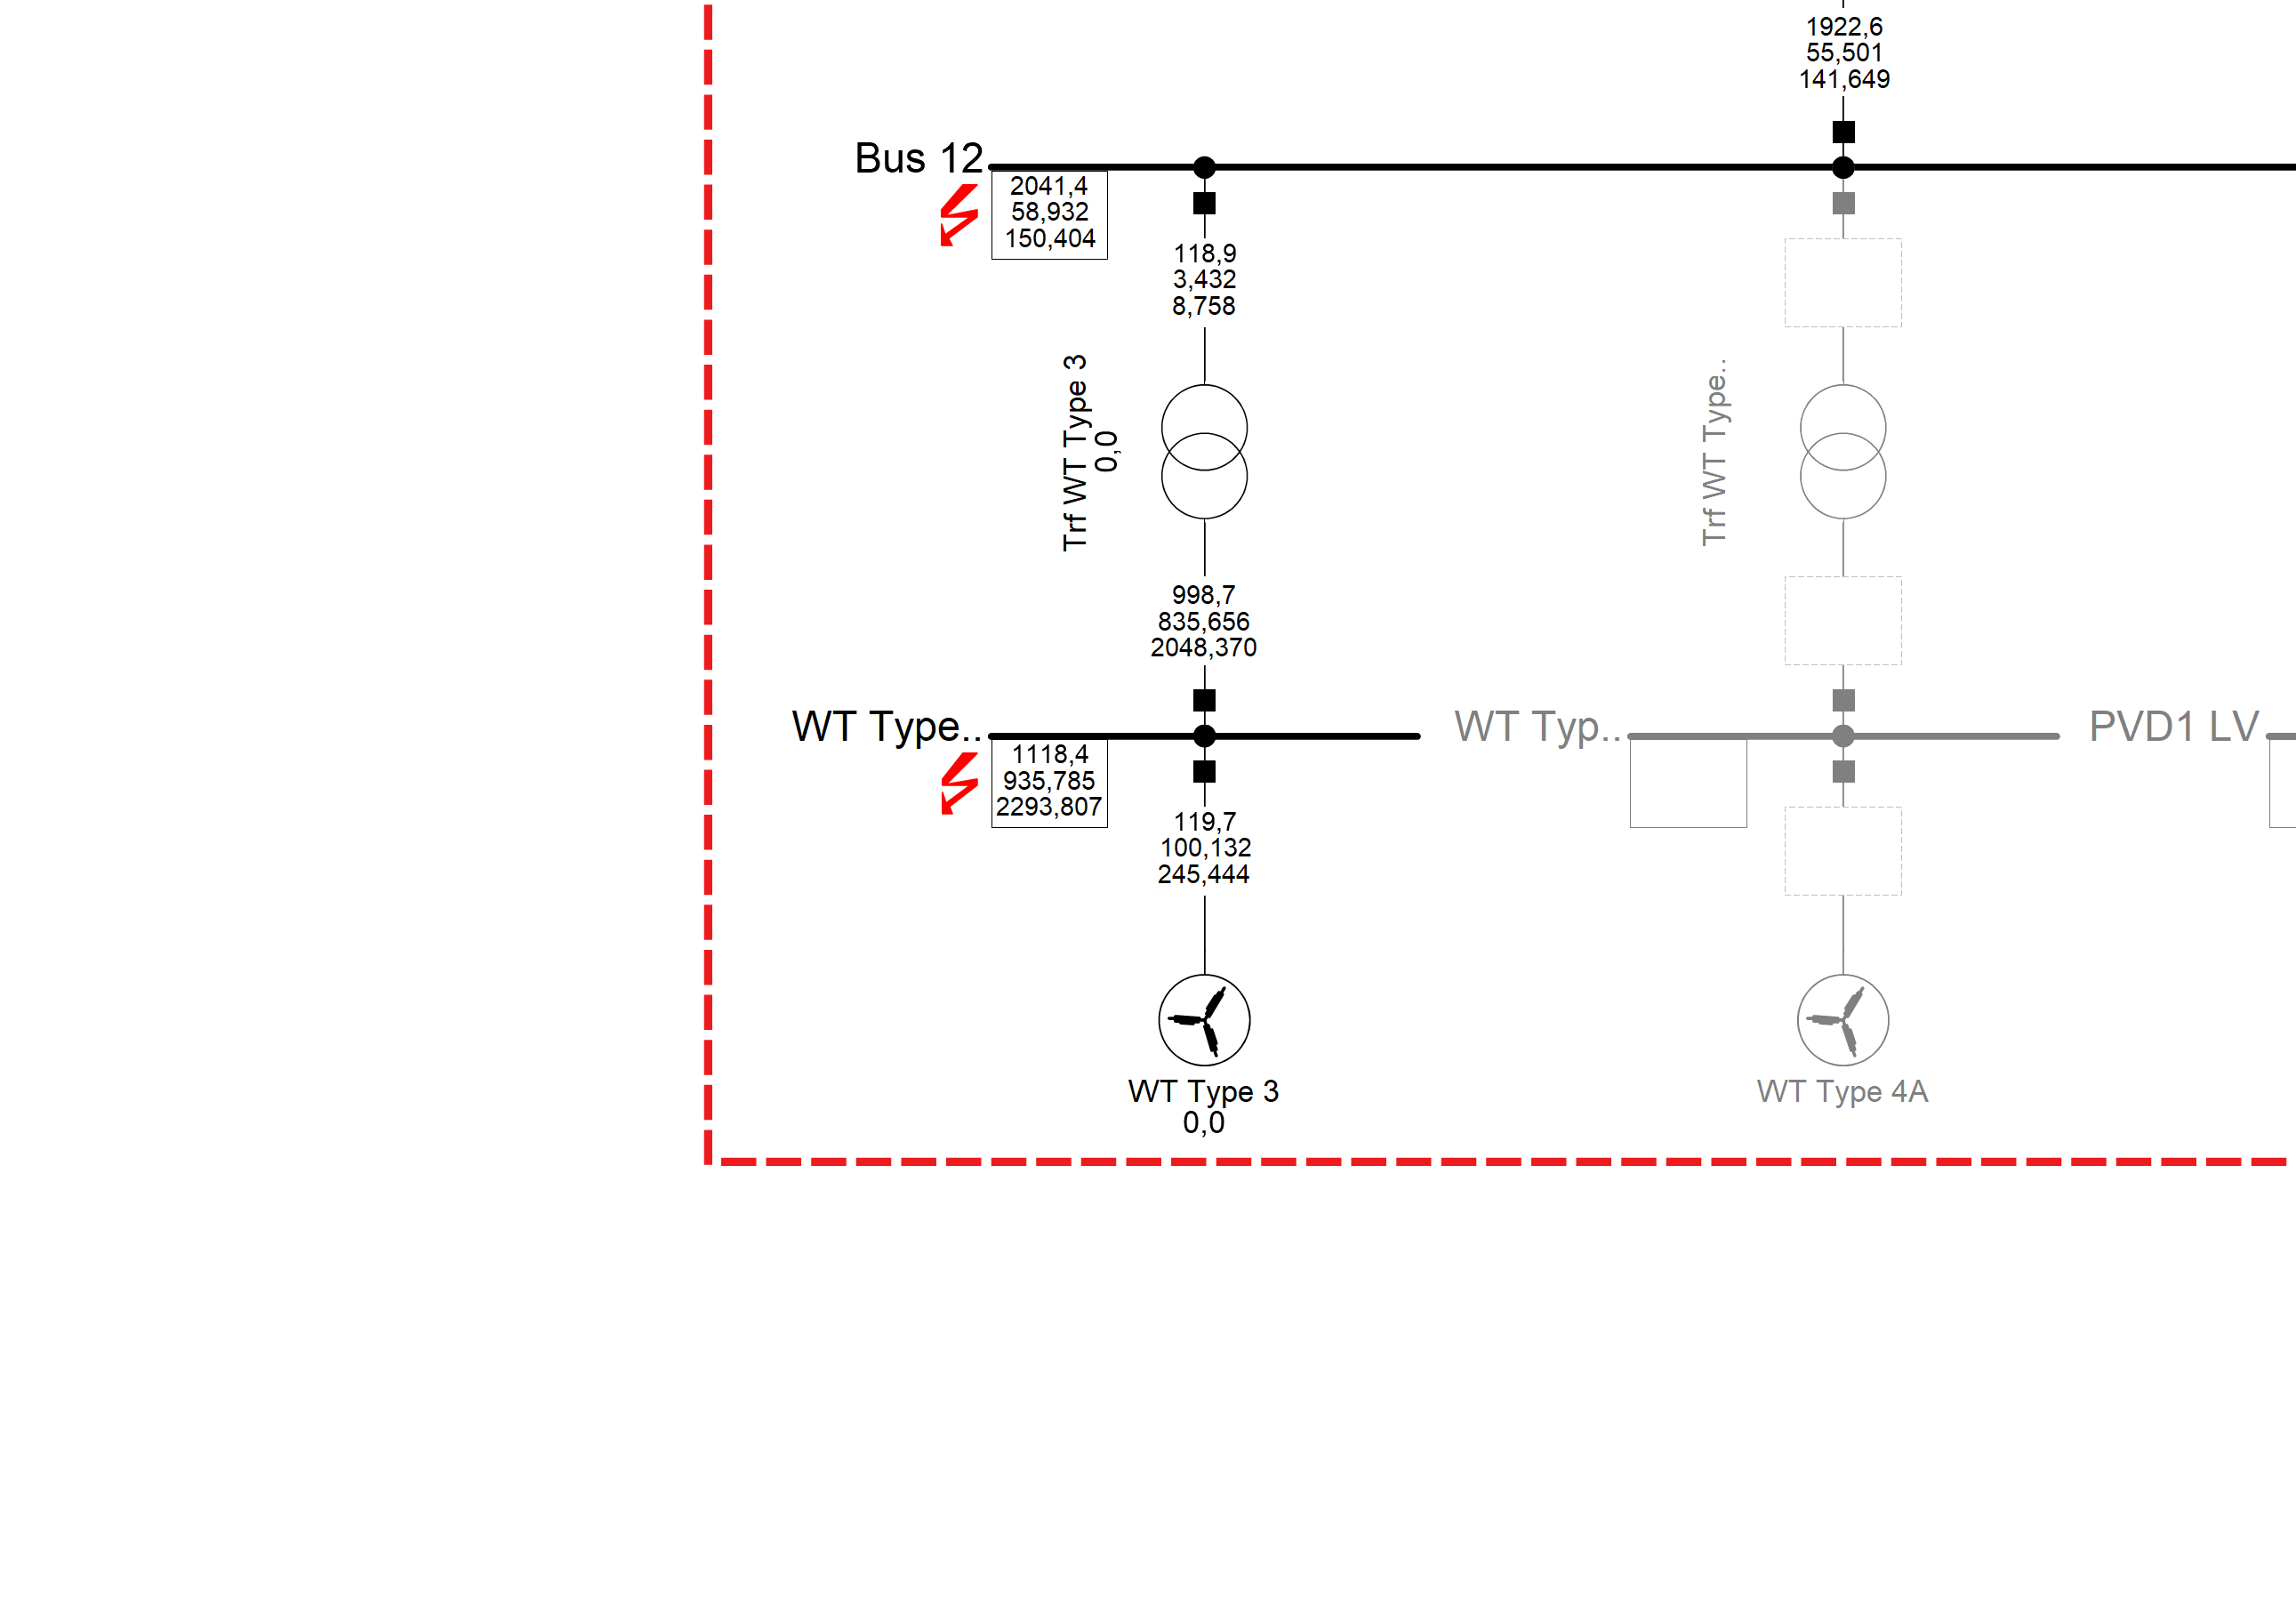
\includegraphics[width=0.8\textwidth]{contents/chapter-4/kontribusi_WTType3.png}
    \caption{Kontribusi Arus Hubung Singkat Wind Turbine Type 3}
    \label{fig:kontribusi_WTType3}
\end{figure}

Berdasarkan hasil simulasi pada Gambar \ref{fig:kontribusi_WTType3}, kontribusi hubung singkat dari \textit{wind turbine type 3} terbaca sebesar 0 MVA. Hasil ini konsisten dengan pengaturan pada Gambar \ref{fig:SC_Setting_WTT3}, karena arus hubung singkat awal maupun tunak pada model ditetapkan sebesar 0 $\mathrm{kA}$. Dengan demikian, WT Type 3 tidak menambah komponen arus gangguan dari sisi IBR terhadap titik gangguan yang dievaluasi.

Implikasinya, respons proteksi pada skenario dengan WT Type 3 tidak dapat dijelaskan sebagai akibat tambahan kontribusi arus hubung singkat dari unit tersebut. Jika pada bagian berikutnya terdapat perubahan pembacaan impedansi tampak, arus diferensial, arus \textit{restraint}, atau keputusan operasi relay, perubahan tersebut perlu dikaitkan dengan konfigurasi jaringan, lokasi gangguan, dan kontribusi dari sumber lain yang masih aktif. Dengan demikian, hasil pada subbagian ini menjadi dasar bahwa pengaruh WT Type 3 pada analisis relay berikutnya bukan berasal dari injeksi arus gangguan tambahan dari unit WT Type 3.

\subsection{Wind Turbine Type 4}

Pembahasan pada model \textit{wind turbine type 4} diawali dari pengaturan hubung singkat yang digunakan pada simulasi. Berbeda dengan WT Type 3 dan PV yang tidak menunjukkan kontribusi arus hubung singkat pada hasil perbandingan ini, model WT Type 4 masih memiliki parameter kontribusi arus gangguan yang aktif. Oleh karena itu, pengaturan pada menu hubung singkat perlu dicermati sebelum hasil kontribusi pada sistem dianalisis.

\begin{figure}[H]
    \centering
    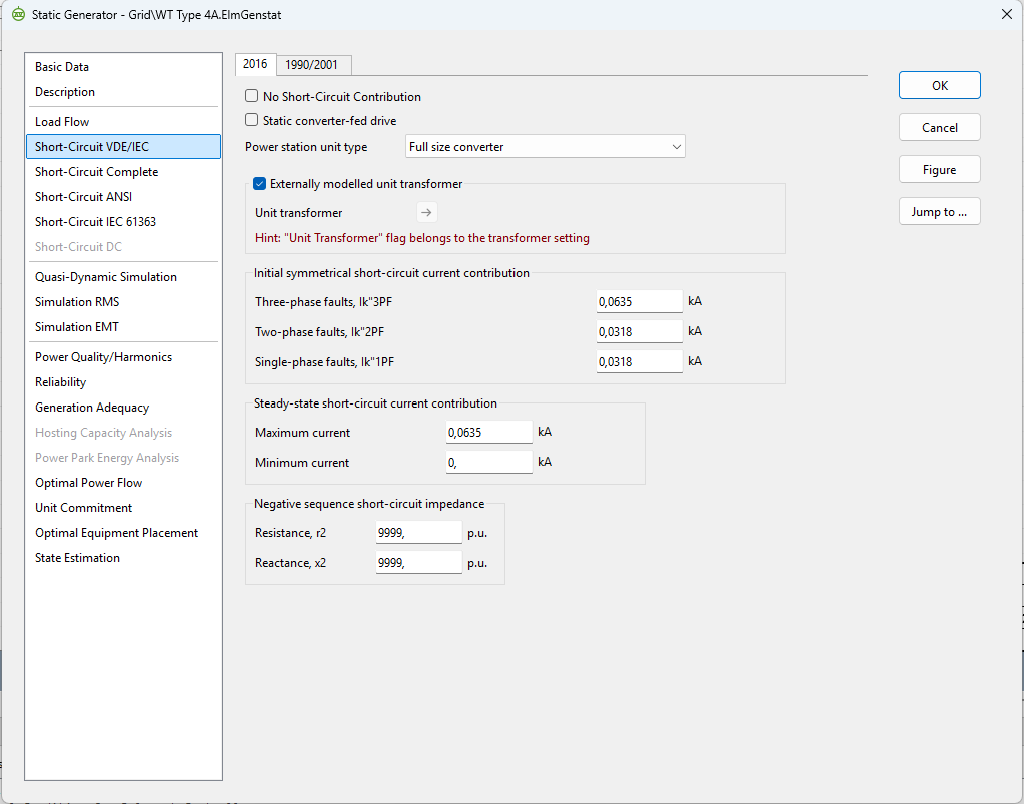
\includegraphics[width=0.8\textwidth]{contents/chapter-4/SC_Setting_WTT4.png}
    \caption{Setting Short Circuit Pada Model Wind Turbine Type 4}
    \label{fig:SC_Setting_WTT4}
\end{figure}

Gambar \ref{fig:SC_Setting_WTT4} menunjukkan bahwa model WT Type 4 pada tab VDE/IEC untuk hubung singkat menggunakan tipe unit \textit{full size converter}. Karakter ini menunjukkan bahwa kontribusi arus gangguan WT Type 4 tidak berasal dari hubungan elektromagnetik langsung antara generator dan jaringan, tetapi dibatasi oleh konverter penuh serta parameter arus gangguan yang dimasukkan pada model. Pada gambar tersebut, opsi \textit{No Short-Circuit Contribution} tidak diaktifkan, sehingga WT Type 4 tetap diperhitungkan sebagai sumber kontribusi hubung singkat dalam simulasi.

Parameter pada Gambar \ref{fig:SC_Setting_WTT4} memperlihatkan bahwa arus hubung singkat awal untuk gangguan tiga fasa ditetapkan sebesar 0,0635 $\mathrm{kA}$, sedangkan untuk gangguan dua fasa dan satu fasa masing-masing sebesar 0,0318 $\mathrm{kA}$. Pada kondisi tunak, arus maksimum ditetapkan sebesar 0,0635 $\mathrm{kA}$ dan arus minimum sebesar 0 $\mathrm{kA}$. Selain itu, impedansi urutan negatif pada parameter $r_2$ dan $x_2$ bernilai sangat besar, yaitu 9999 p.u. Kombinasi pengaturan ini menunjukkan bahwa kontribusi WT Type 4 tetap ada, tetapi besar dan karakteristiknya dibatasi oleh model konverter penuh.

\begin{figure}[H]
    \centering
    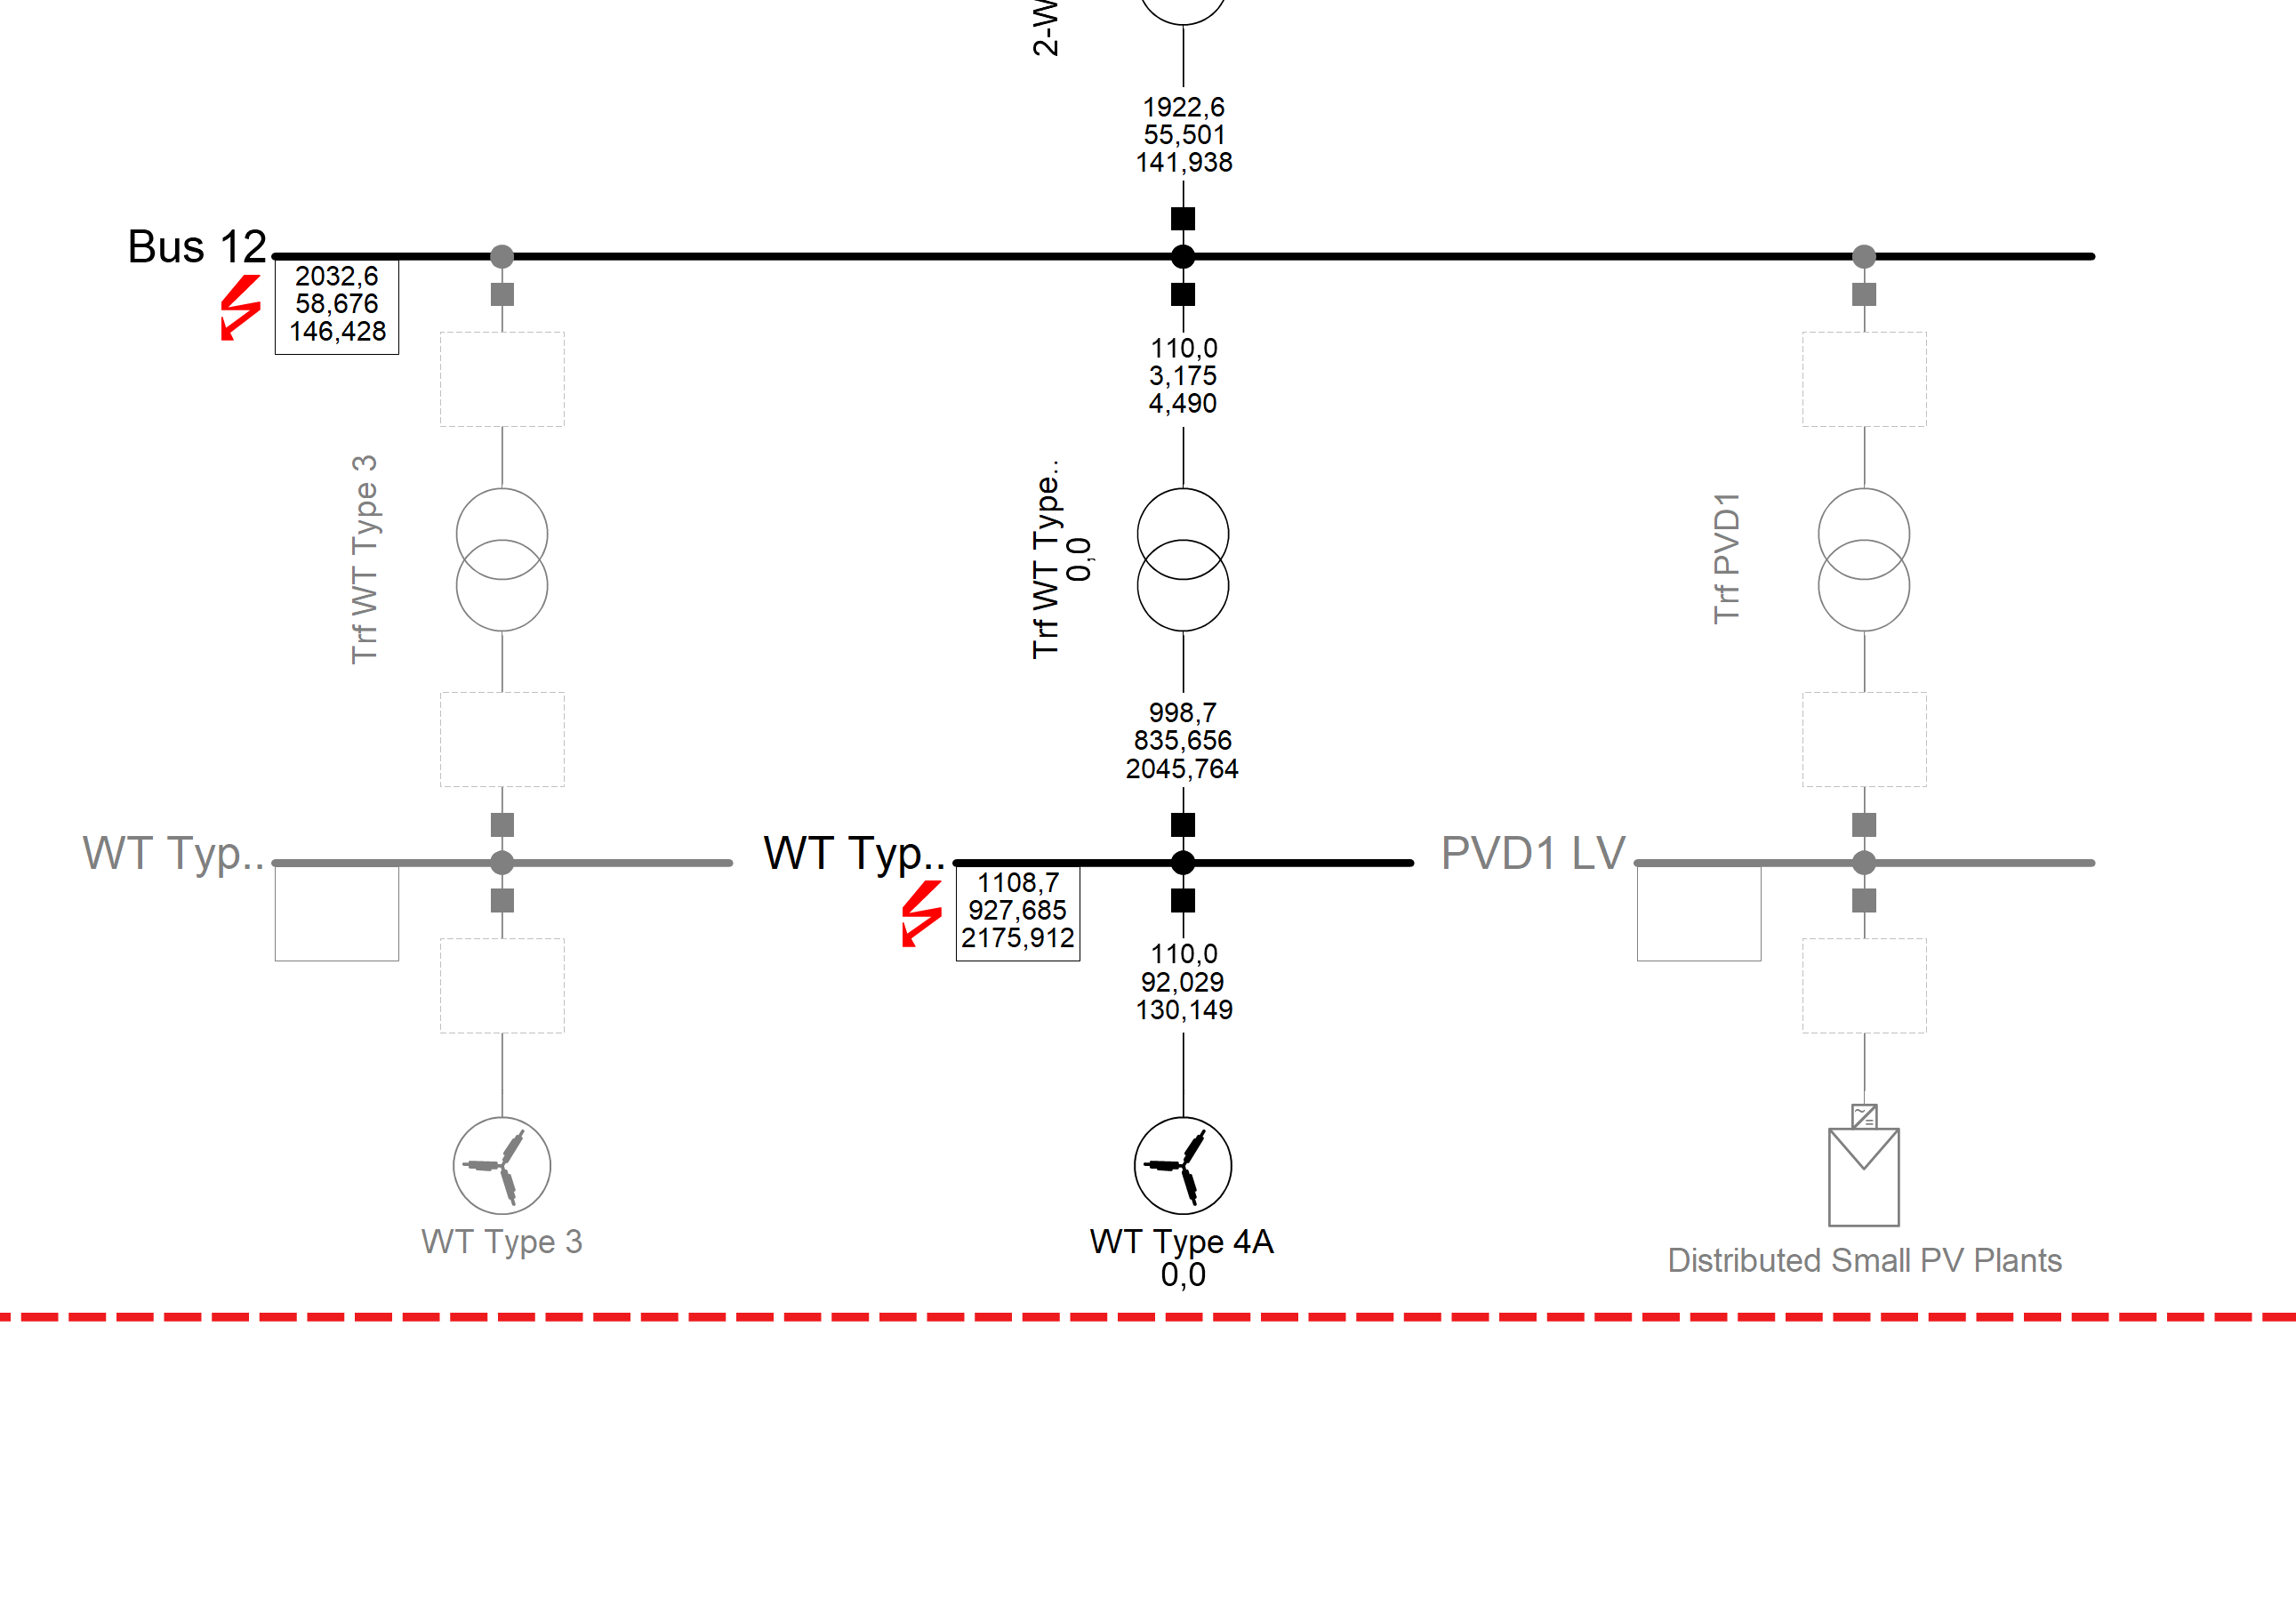
\includegraphics[width=0.8\textwidth]{contents/chapter-4/kontribusi_WTType4.png}
    \caption{Kontribusi Arus Hubung Singkat Wind Turbine Type 4}
    \label{fig:kontribusi_WTType4}
\end{figure}

Berdasarkan hasil simulasi pada Gambar \ref{fig:kontribusi_WTType4}, \textit{wind turbine type 4} memberikan kontribusi hubung singkat sebesar 110 MVA atau setara dengan 1,1 p.u. Hasil ini konsisten dengan pengaturan pada Gambar \ref{fig:SC_Setting_WTT4}, karena opsi kontribusi hubung singkat tidak dinonaktifkan dan model masih memiliki batas arus gangguan yang didefinisikan.

Selain dalam satuan daya hubung singkat, Gambar \ref{fig:kontribusi_WTType4} juga menunjukkan kontribusi arus hubung singkat sebesar 92,029 $\mathrm{kA}$ atau 1,14 p.u. Nilai ini menegaskan bahwa WT Type 4 masih menyuplai arus gangguan pada kondisi yang diuji. Dengan demikian, WT Type 4 menjadi jenis IBR yang perlu mendapat perhatian khusus pada analisis relay berikutnya, karena kontribusi arus gangguannya dapat memengaruhi besaran yang terbaca oleh relay 21 maupun relay 87L.

Implikasinya, respons proteksi pada skenario dengan WT Type 4 tidak dapat dibaca dengan asumsi bahwa sumber IBR tidak menyuplai arus gangguan. Berbeda dengan WT Type 3 dan PV yang menunjukkan kontribusi 0 MVA, WT Type 4 memberikan tambahan kontribusi hubung singkat yang dapat memengaruhi arus gangguan, impedansi tampak, arus diferensial, dan arus \textit{restraint}. Oleh karena itu, hasil pada subbagian ini menjadi dasar untuk membaca perubahan respons relay pada skenario yang melibatkan WT Type 4.

\subsection{Photovoltaic}

Pembahasan pada model \textit{photovoltaic} diawali dari pengaturan kontribusi hubung singkat yang digunakan pada simulasi. Hal ini diperlukan karena hasil kontribusi arus gangguan dari PV tidak hanya dipengaruhi oleh jenis sumbernya, tetapi juga oleh opsi pemodelan yang diaktifkan pada menu hubung singkat.

\begin{figure}[H]
    \centering
    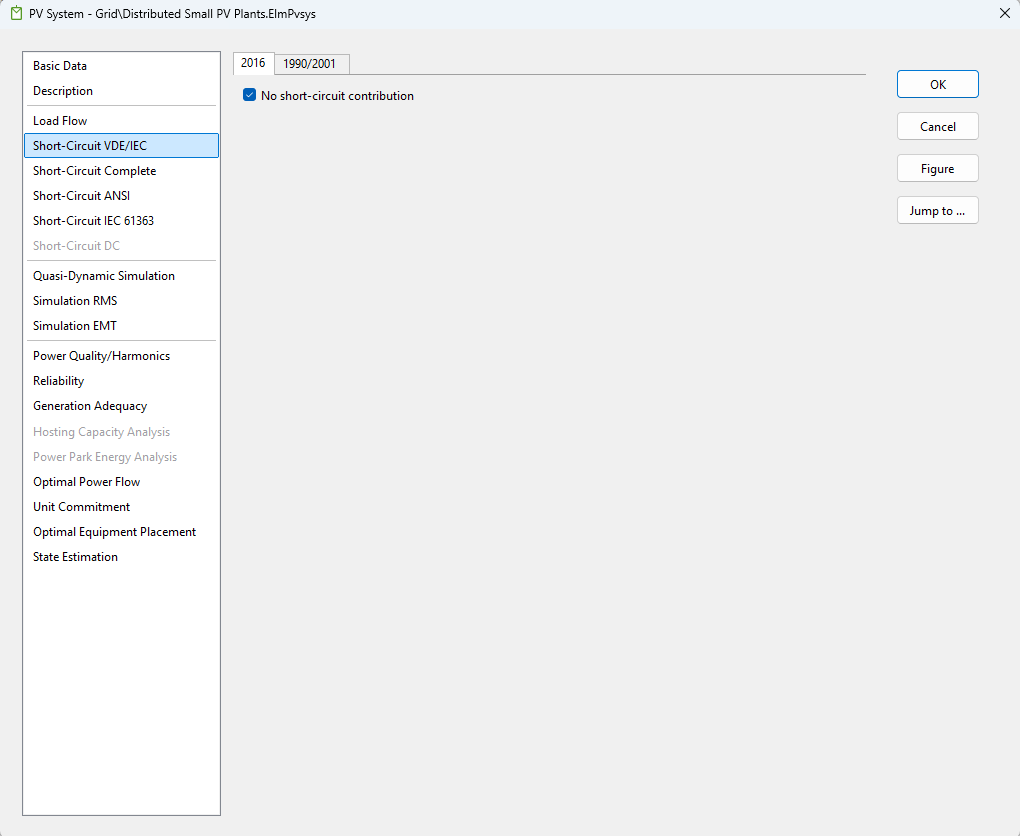
\includegraphics[width=0.8\textwidth]{contents/chapter-4/SC_Setting_PV.png}
    \caption{Setting Short Circuit Pada Model Photovoltaic}
    \label{fig:SC_Setting_PV}
\end{figure}

Gambar \ref{fig:SC_Setting_PV} menunjukkan bahwa pada tab VDE/IEC untuk hubung singkat, opsi \textit{No short-circuit contribution} berada dalam keadaan aktif. Dengan pengaturan tersebut, model \textit{photovoltaic} tidak diperhitungkan sebagai sumber kontribusi arus hubung singkat pada perhitungan gangguan. Artinya, arus gangguan dari sisi PV sengaja tidak dimasukkan ke dalam kalkulasi hubung singkat yang digunakan pada bagian ini.

Konsekuensi dari pengaturan tersebut adalah model PV tidak memiliki parameter kontribusi arus hubung singkat yang aktif seperti pada model WT Type 4. Oleh karena itu, sebelum membaca hasil kontribusi pada gambar berikutnya, perlu dipahami bahwa nilai yang muncul merupakan dampak langsung dari opsi pemodelan pada Gambar \ref{fig:SC_Setting_PV}, bukan akibat keterbatasan pembacaan hasil simulasi.

\begin{figure}[H]
    \centering
    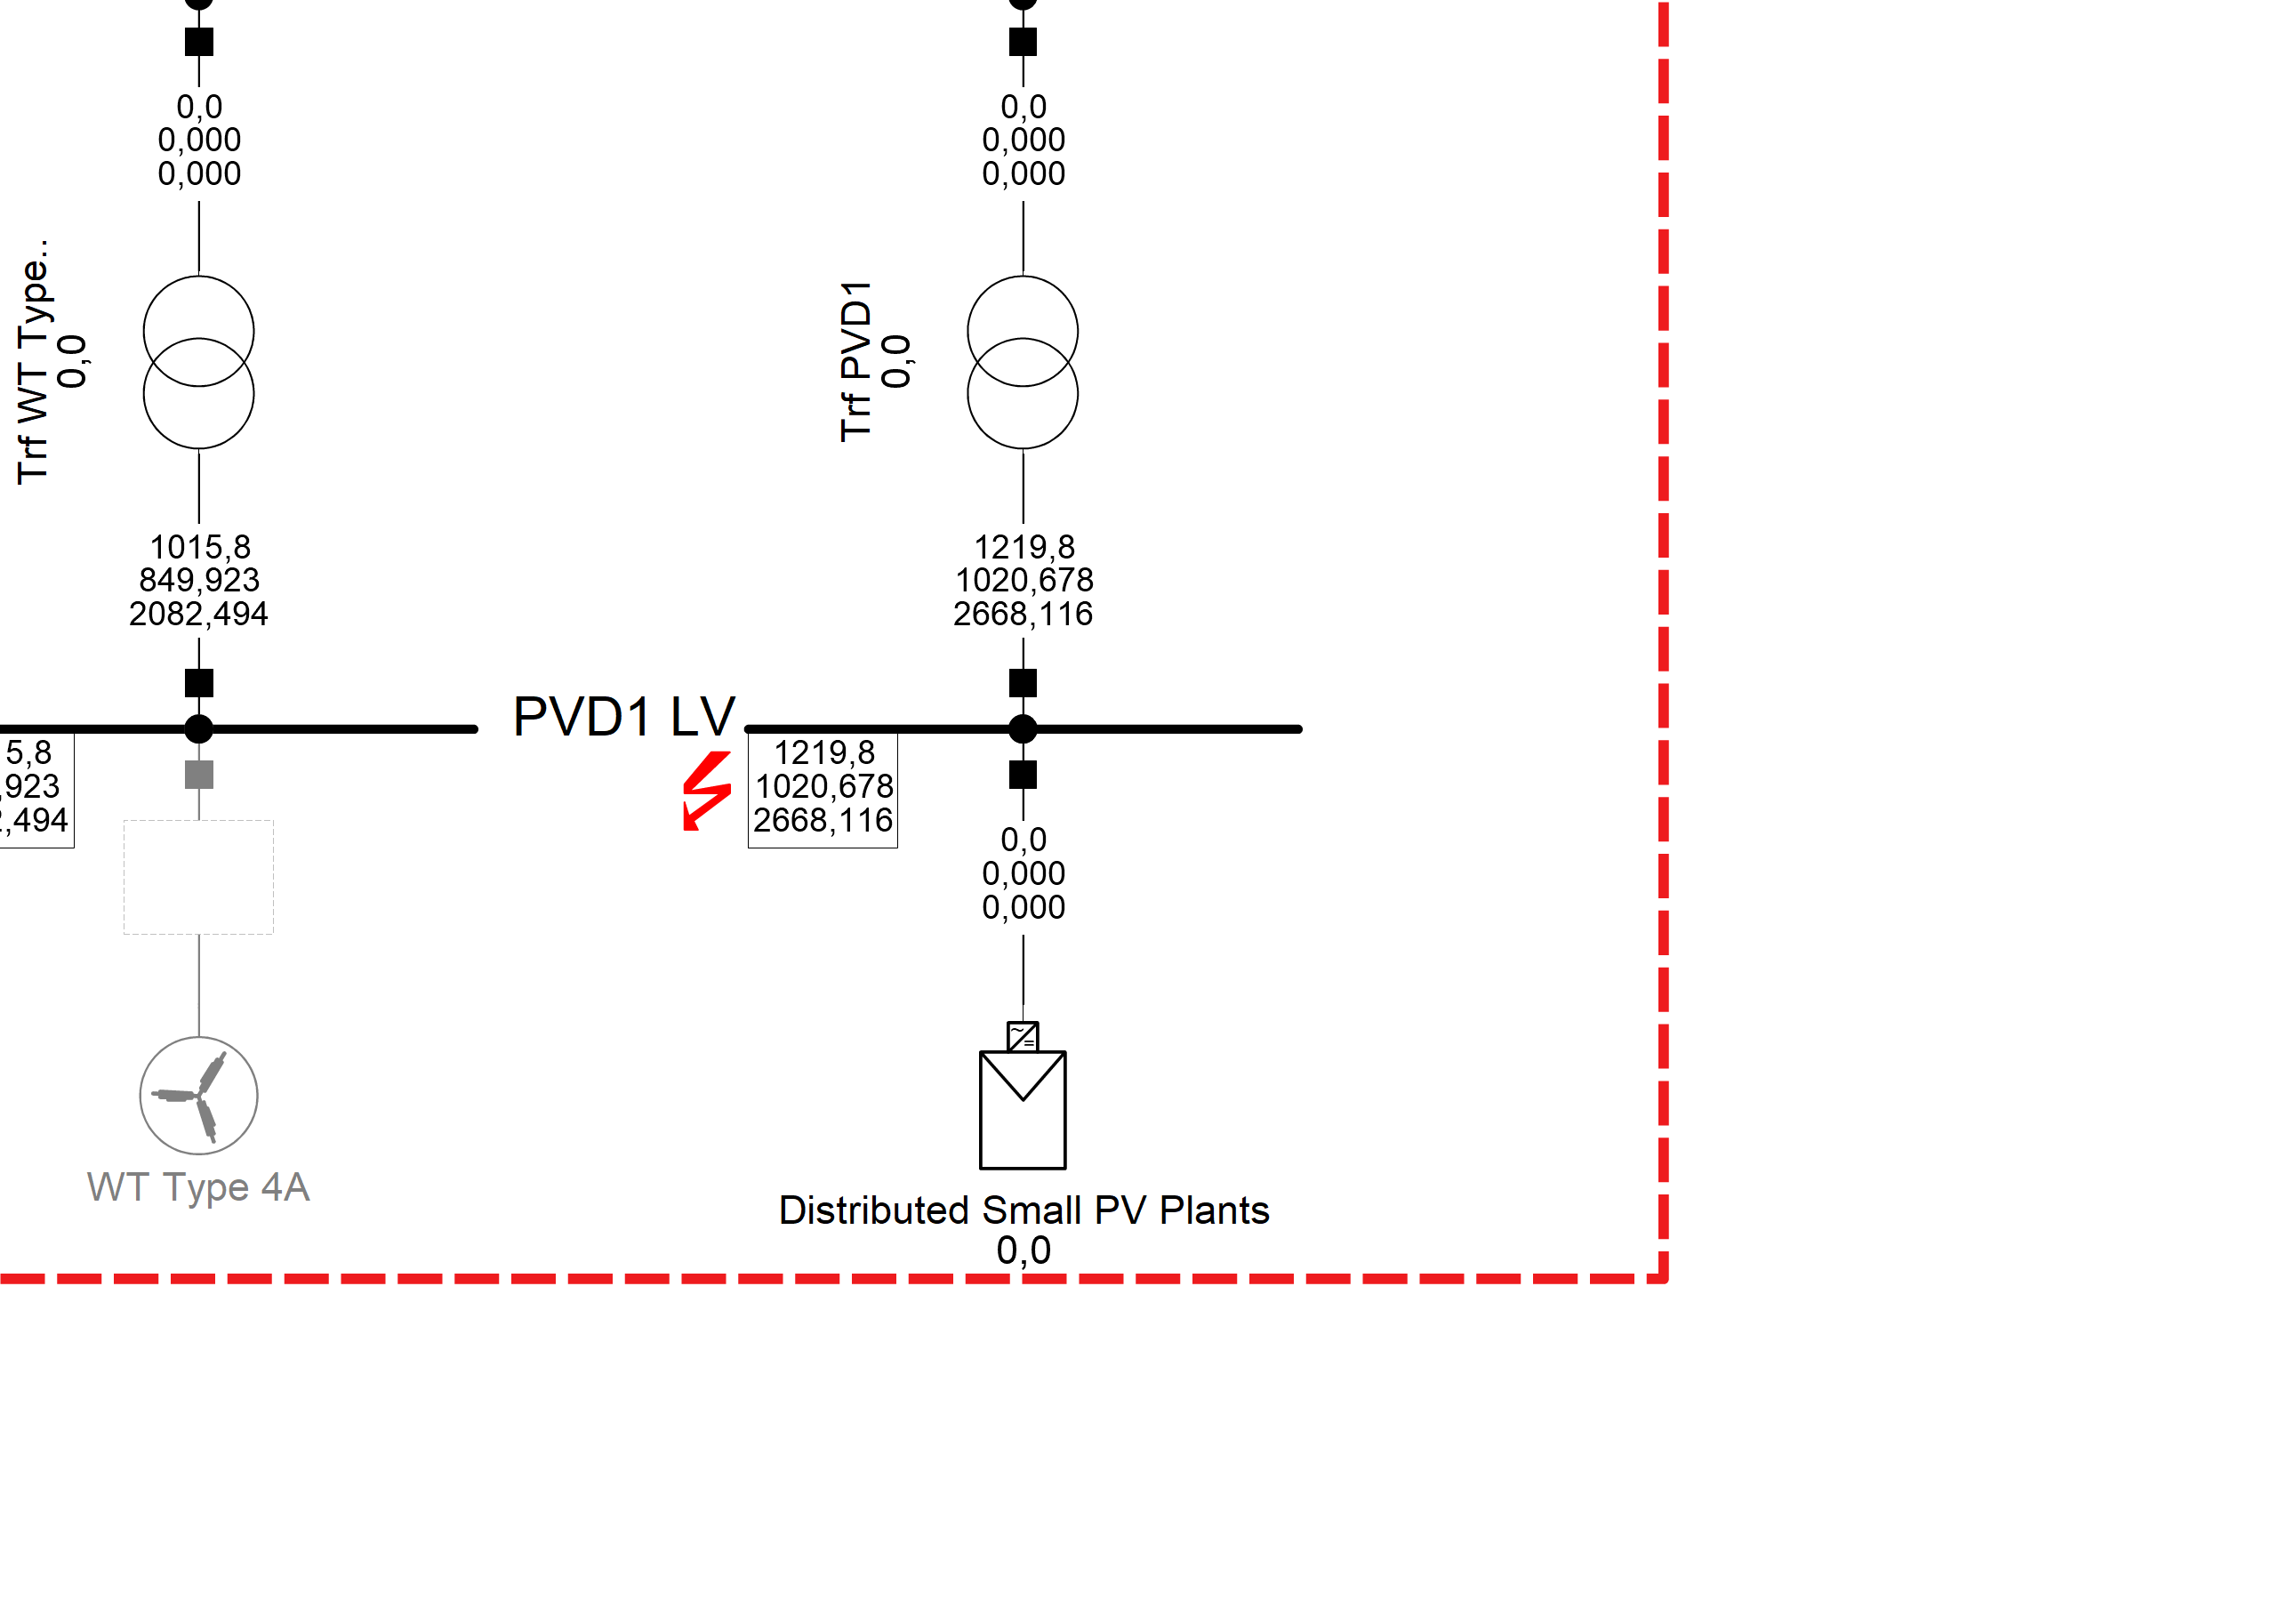
\includegraphics[width=0.8\textwidth]{contents/chapter-4/kontribusi_PV.png}
    \caption{Kontribusi Arus Hubung Singkat Photovoltaic}
    \label{fig:kontribusi_PV}
\end{figure}

Berdasarkan hasil simulasi pada Gambar \ref{fig:kontribusi_PV}, kontribusi hubung singkat dari \textit{photovoltaic} terbaca sebesar 0 MVA. Hasil ini konsisten dengan pengaturan sebelumnya, karena opsi \textit{No short-circuit contribution} membuat unit PV tidak menyuplai arus gangguan tambahan ke sistem. Dengan demikian, pada skenario ini PV berperan sebagai sumber yang terhubung pada sistem, tetapi tidak menjadi penyumbang arus hubung singkat dalam perhitungan gangguan.

Implikasinya, respons relay pada skenario dengan \textit{photovoltaic} tidak dapat dijelaskan sebagai akibat tambahan kontribusi arus hubung singkat dari sisi PV. Jika pada bagian berikutnya terdapat perubahan pembacaan impedansi tampak, arus diferensial, arus \textit{restraint}, atau keputusan operasi relay, perubahan tersebut perlu dikaitkan dengan konfigurasi jaringan, lokasi gangguan, dan besaran listrik yang terbaca pada terminal relay. Dengan demikian, hasil pada subbagian ini menjadi dasar bahwa pengaruh PV pada analisis relay berikutnya tidak berasal dari injeksi arus gangguan tambahan dari unit PV.

\section{Dekomposisi Komponen Urutan Arus pada Setiap Skenario}

\subsection{Kondisi Tanpa Integrasi IBR}

\subsubsection{Gangguan Internal Double Line-to-Ground Fault}

Subbagian ini membahas perubahan komponen arus urutan pada saluran TL89 untuk kondisi sistem tanpa integrasi IBR saat terjadi gangguan internal \textit{double line-to-ground}. Pembahasan difokuskan pada komponen urutan positif, negatif, dan nol, karena ketiga komponen tersebut menunjukkan pola ketidakseimbangan arus yang muncul selama gangguan dua fasa ke tanah.

\begin{figure}[H]
    \centering
    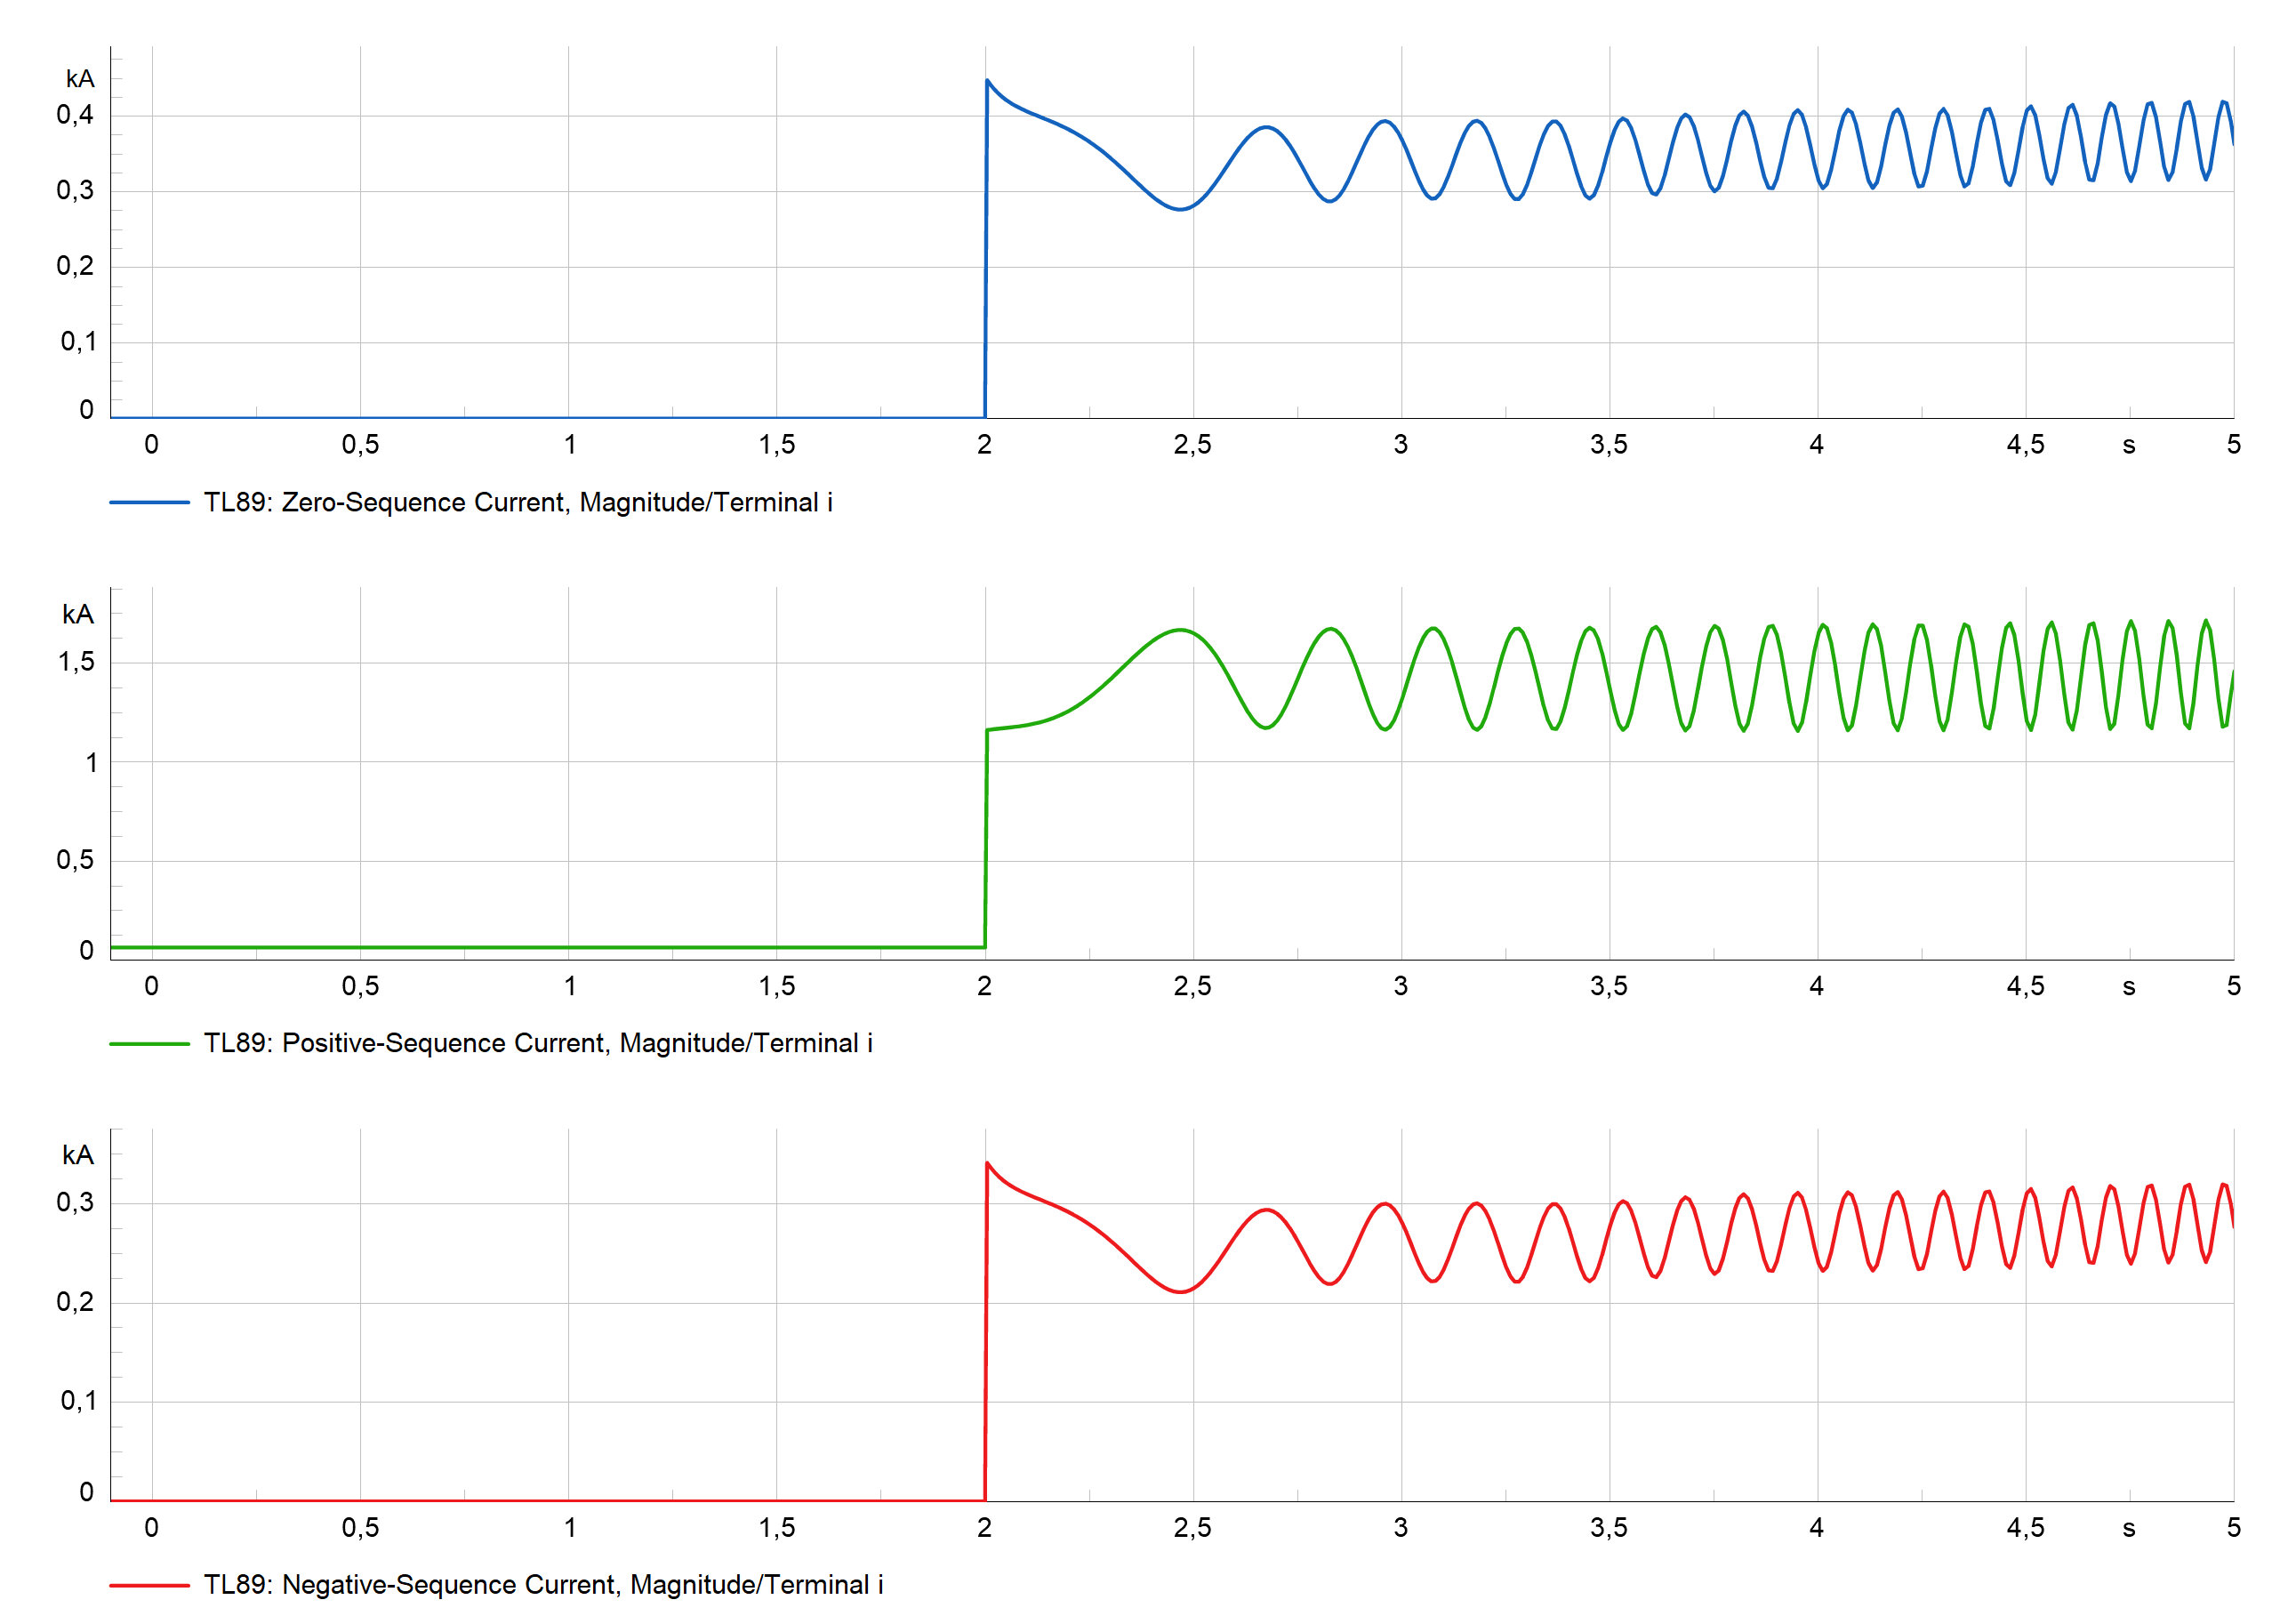
\includegraphics[width=0.8\textwidth]{contents/chapter-4/TL89_seq_internal_dlg.png}
    \caption{Dekomposisi Komponen Urutan Arus pada Gangguan Internal Double Line-to-Ground}
    \label{fig:TL89_seq_internal_dlg}
\end{figure}

Berdasarkan Gambar \ref{fig:TL89_seq_internal_dlg}, gangguan internal \textit{double line-to-ground} menyebabkan peningkatan pada komponen arus urutan positif, negatif, dan nol. Komponen urutan positif naik dari 0,063 kA menjadi sekitar 1,163 kA sesaat setelah gangguan terjadi, kemudian berosilasi pada rentang 1,17 - 1,705 kA. Pada saat yang sama, komponen urutan negatif meningkat dari 0 kA menjadi sekitar 0,3411 kA, lalu berosilasi pada rentang 0,2395 - 0,3115 kA. Komponen urutan nol juga menunjukkan peningkatan dari 0 kA menjadi sekitar 0,45 kA, kemudian berosilasi pada rentang 0,3142 - 0,4087 kA.

Peningkatan ketiga komponen tersebut menunjukkan adanya ketidakseimbangan arus yang signifikan akibat gangguan. Komponen urutan positif meningkat karena adanya arus yang mengalir melalui jalur gangguan, sedangkan komponen urutan negatif dan nol meningkat akibat ketidakseimbangan arus pada gangguan dua fasa ke tanah. Dengan demikian, pola kenaikan komponen urutan pada Gambar \ref{fig:TL89_seq_internal_dlg} memperlihatkan karakteristik gangguan internal \textit{double line-to-ground} pada saluran TL89.

\subsubsection{Gangguan External 3-Phase Fault}

Subbagian ini membahas perubahan komponen arus urutan pada saluran TL89 untuk kondisi sistem tanpa integrasi IBR saat terjadi gangguan external \textit{3-phase fault}. Pembahasan difokuskan pada respons komponen urutan positif, negatif, dan nol untuk melihat pola arus yang muncul pada saluran selama gangguan berlangsung.

\begin{figure}[H]
    \centering
    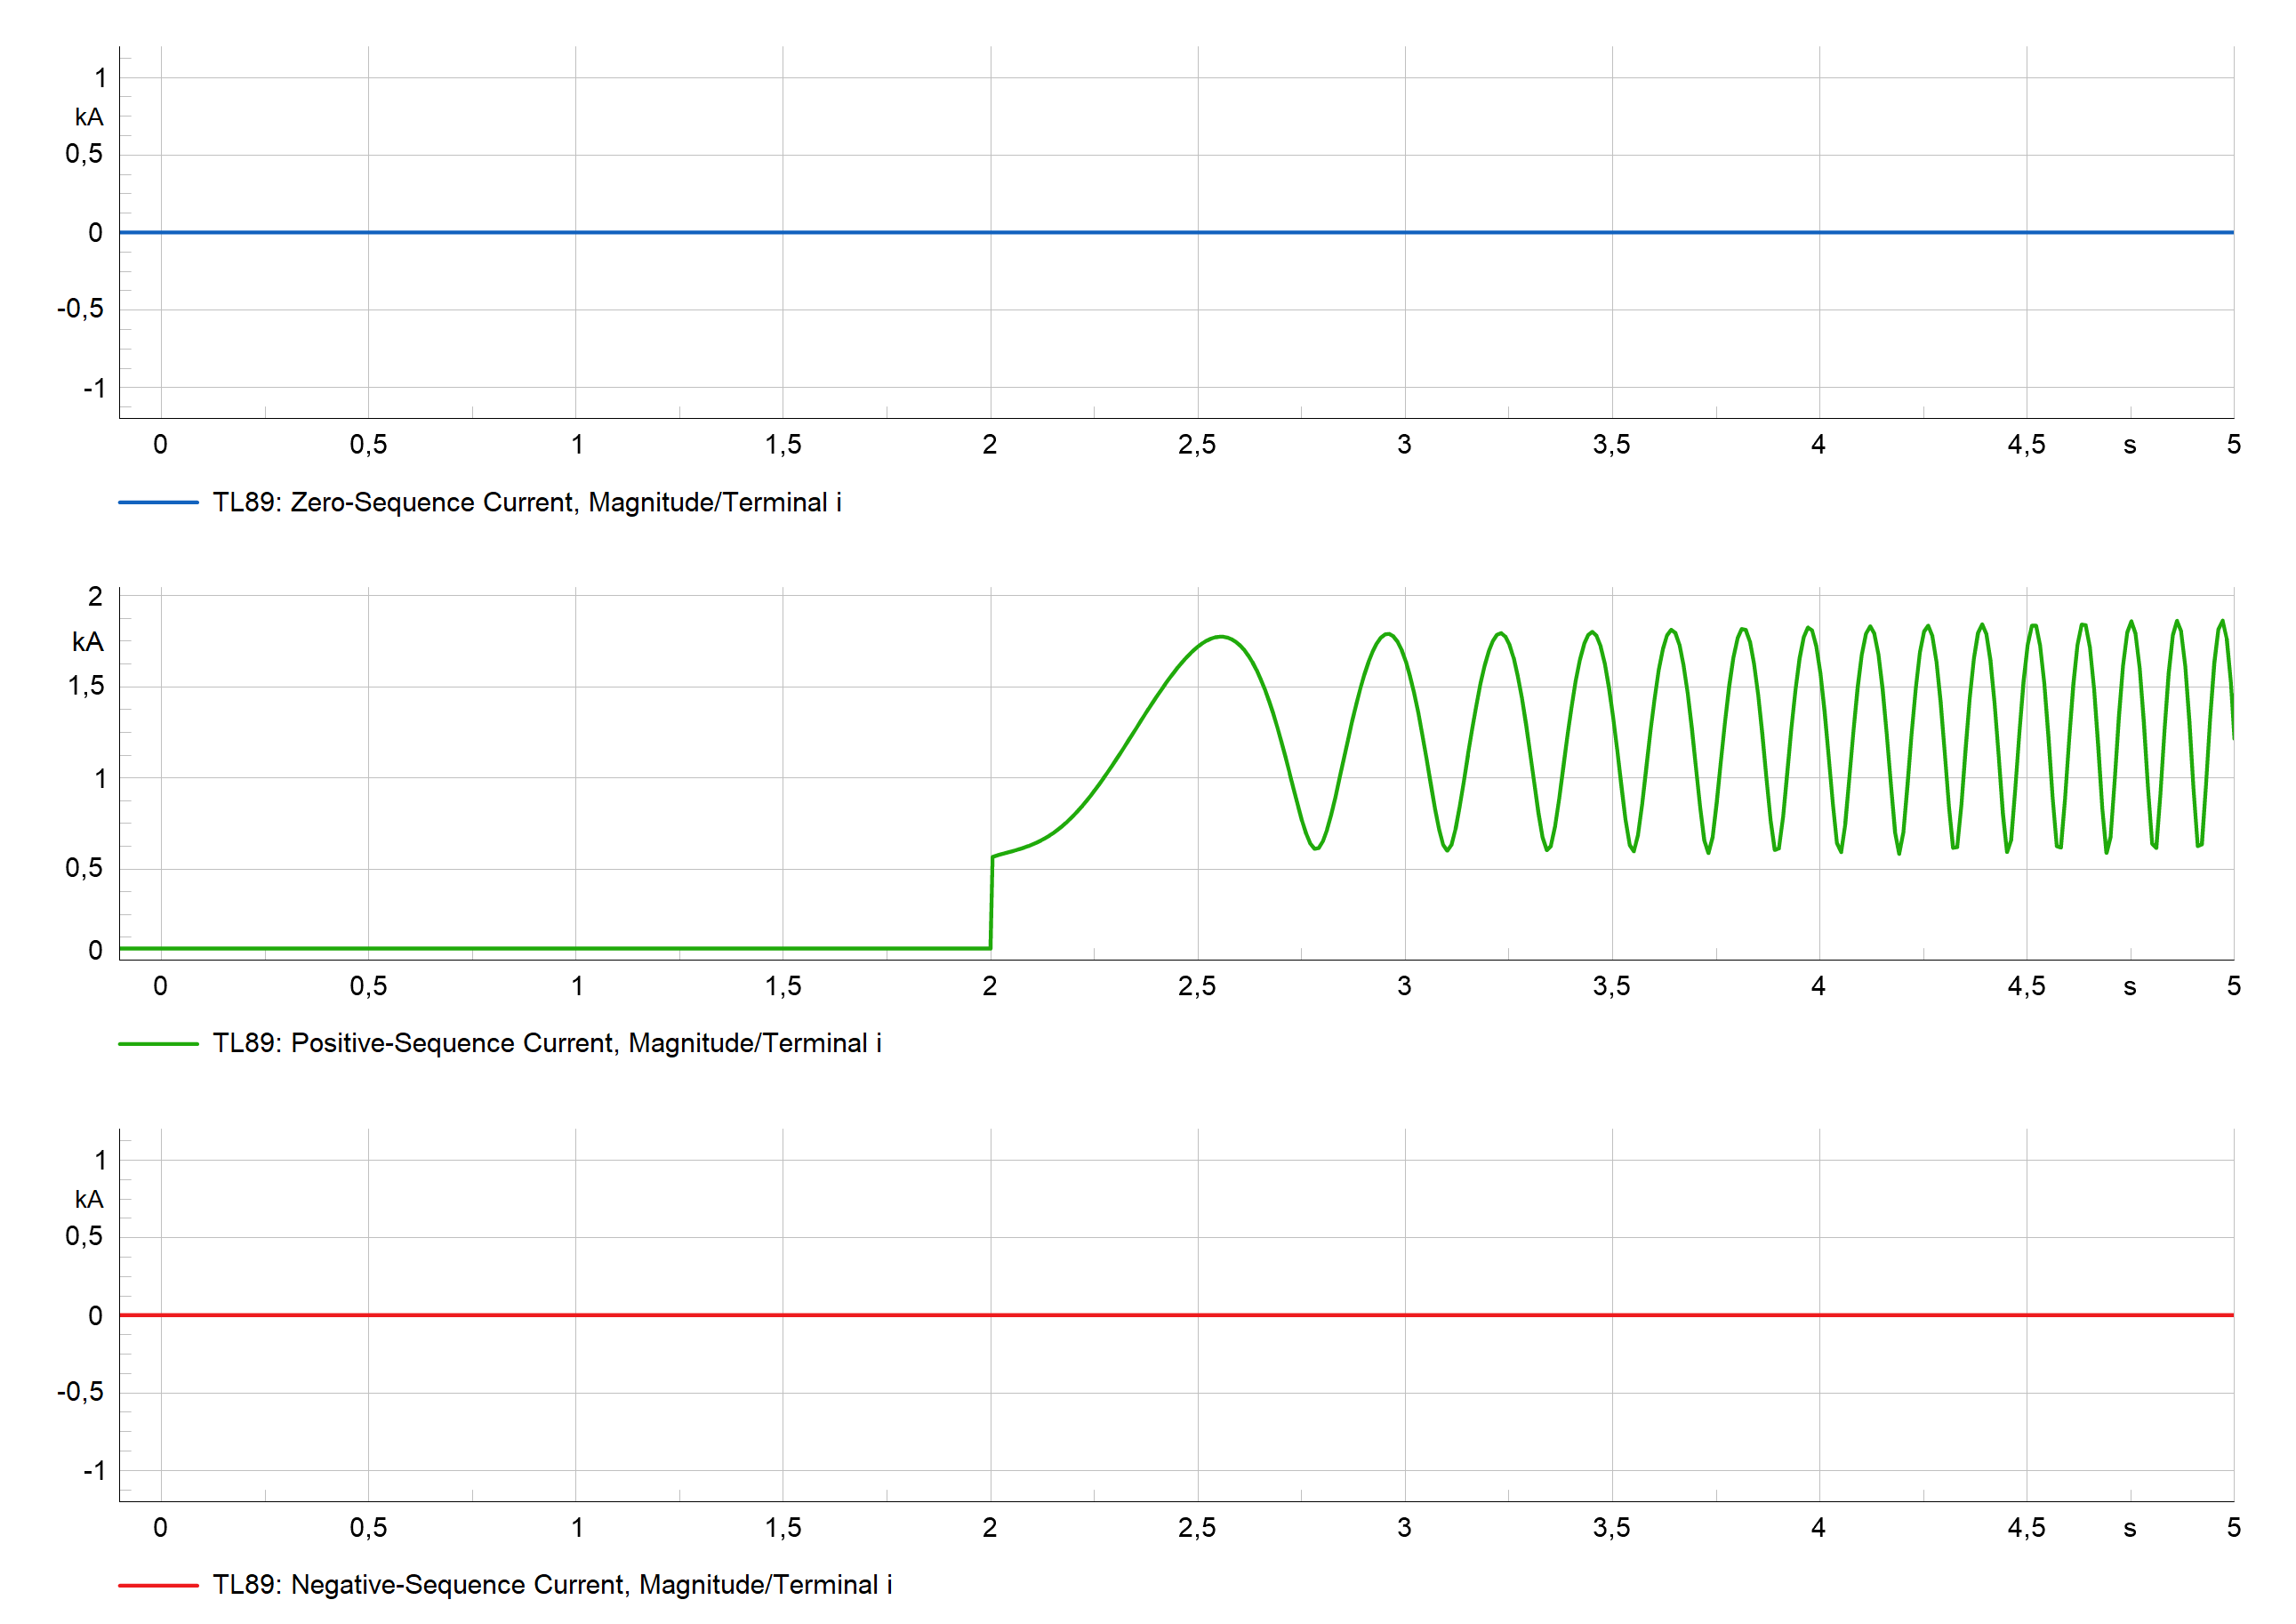
\includegraphics[width=0.8\textwidth]{contents/chapter-4/TL89_seq_external_3p.png}
    \caption{Dekomposisi Komponen Urutan Arus pada Gangguan External 3-Phase Fault}
    \label{fig:TL89_seq_external_3p}
\end{figure}

Berdasarkan Gambar \ref{fig:TL89_seq_external_3p}, gangguan external \textit{3-phase fault} menyebabkan peningkatan pada komponen arus urutan positif. Nilainya naik dari 0,063 kA menjadi sekitar 0,57 kA sesaat setelah gangguan terjadi, kemudian berosilasi pada rentang 0,61 - 1,84 kA. Sementara itu, komponen urutan negatif dan nol tidak mengalami perubahan, karena keduanya tetap bernilai nol selama kondisi gangguan tersebut.

Peningkatan komponen urutan positif menunjukkan adanya perubahan arus yang signifikan, karena arus mengalir melalui jalur gangguan. Tidak munculnya perubahan pada komponen urutan negatif dan nol memperlihatkan bahwa pola arus pada kasus ini didominasi oleh komponen urutan positif. Dengan demikian, hasil pada Gambar \ref{fig:TL89_seq_external_3p} menunjukkan karakteristik gangguan external \textit{3-phase fault} pada saluran TL89.

\subsubsection{Gangguan External Single Line-to-Ground Fault}

Subbagian ini membahas perubahan komponen arus urutan pada saluran TL89 untuk kondisi sistem tanpa integrasi IBR saat terjadi gangguan external \textit{single line-to-ground}. Pembahasan difokuskan pada komponen urutan positif, negatif, dan nol, karena gangguan satu fasa ke tanah menimbulkan ketidakseimbangan arus yang dapat terlihat pada ketiga komponen tersebut.

\begin{figure}[H]
    \centering
    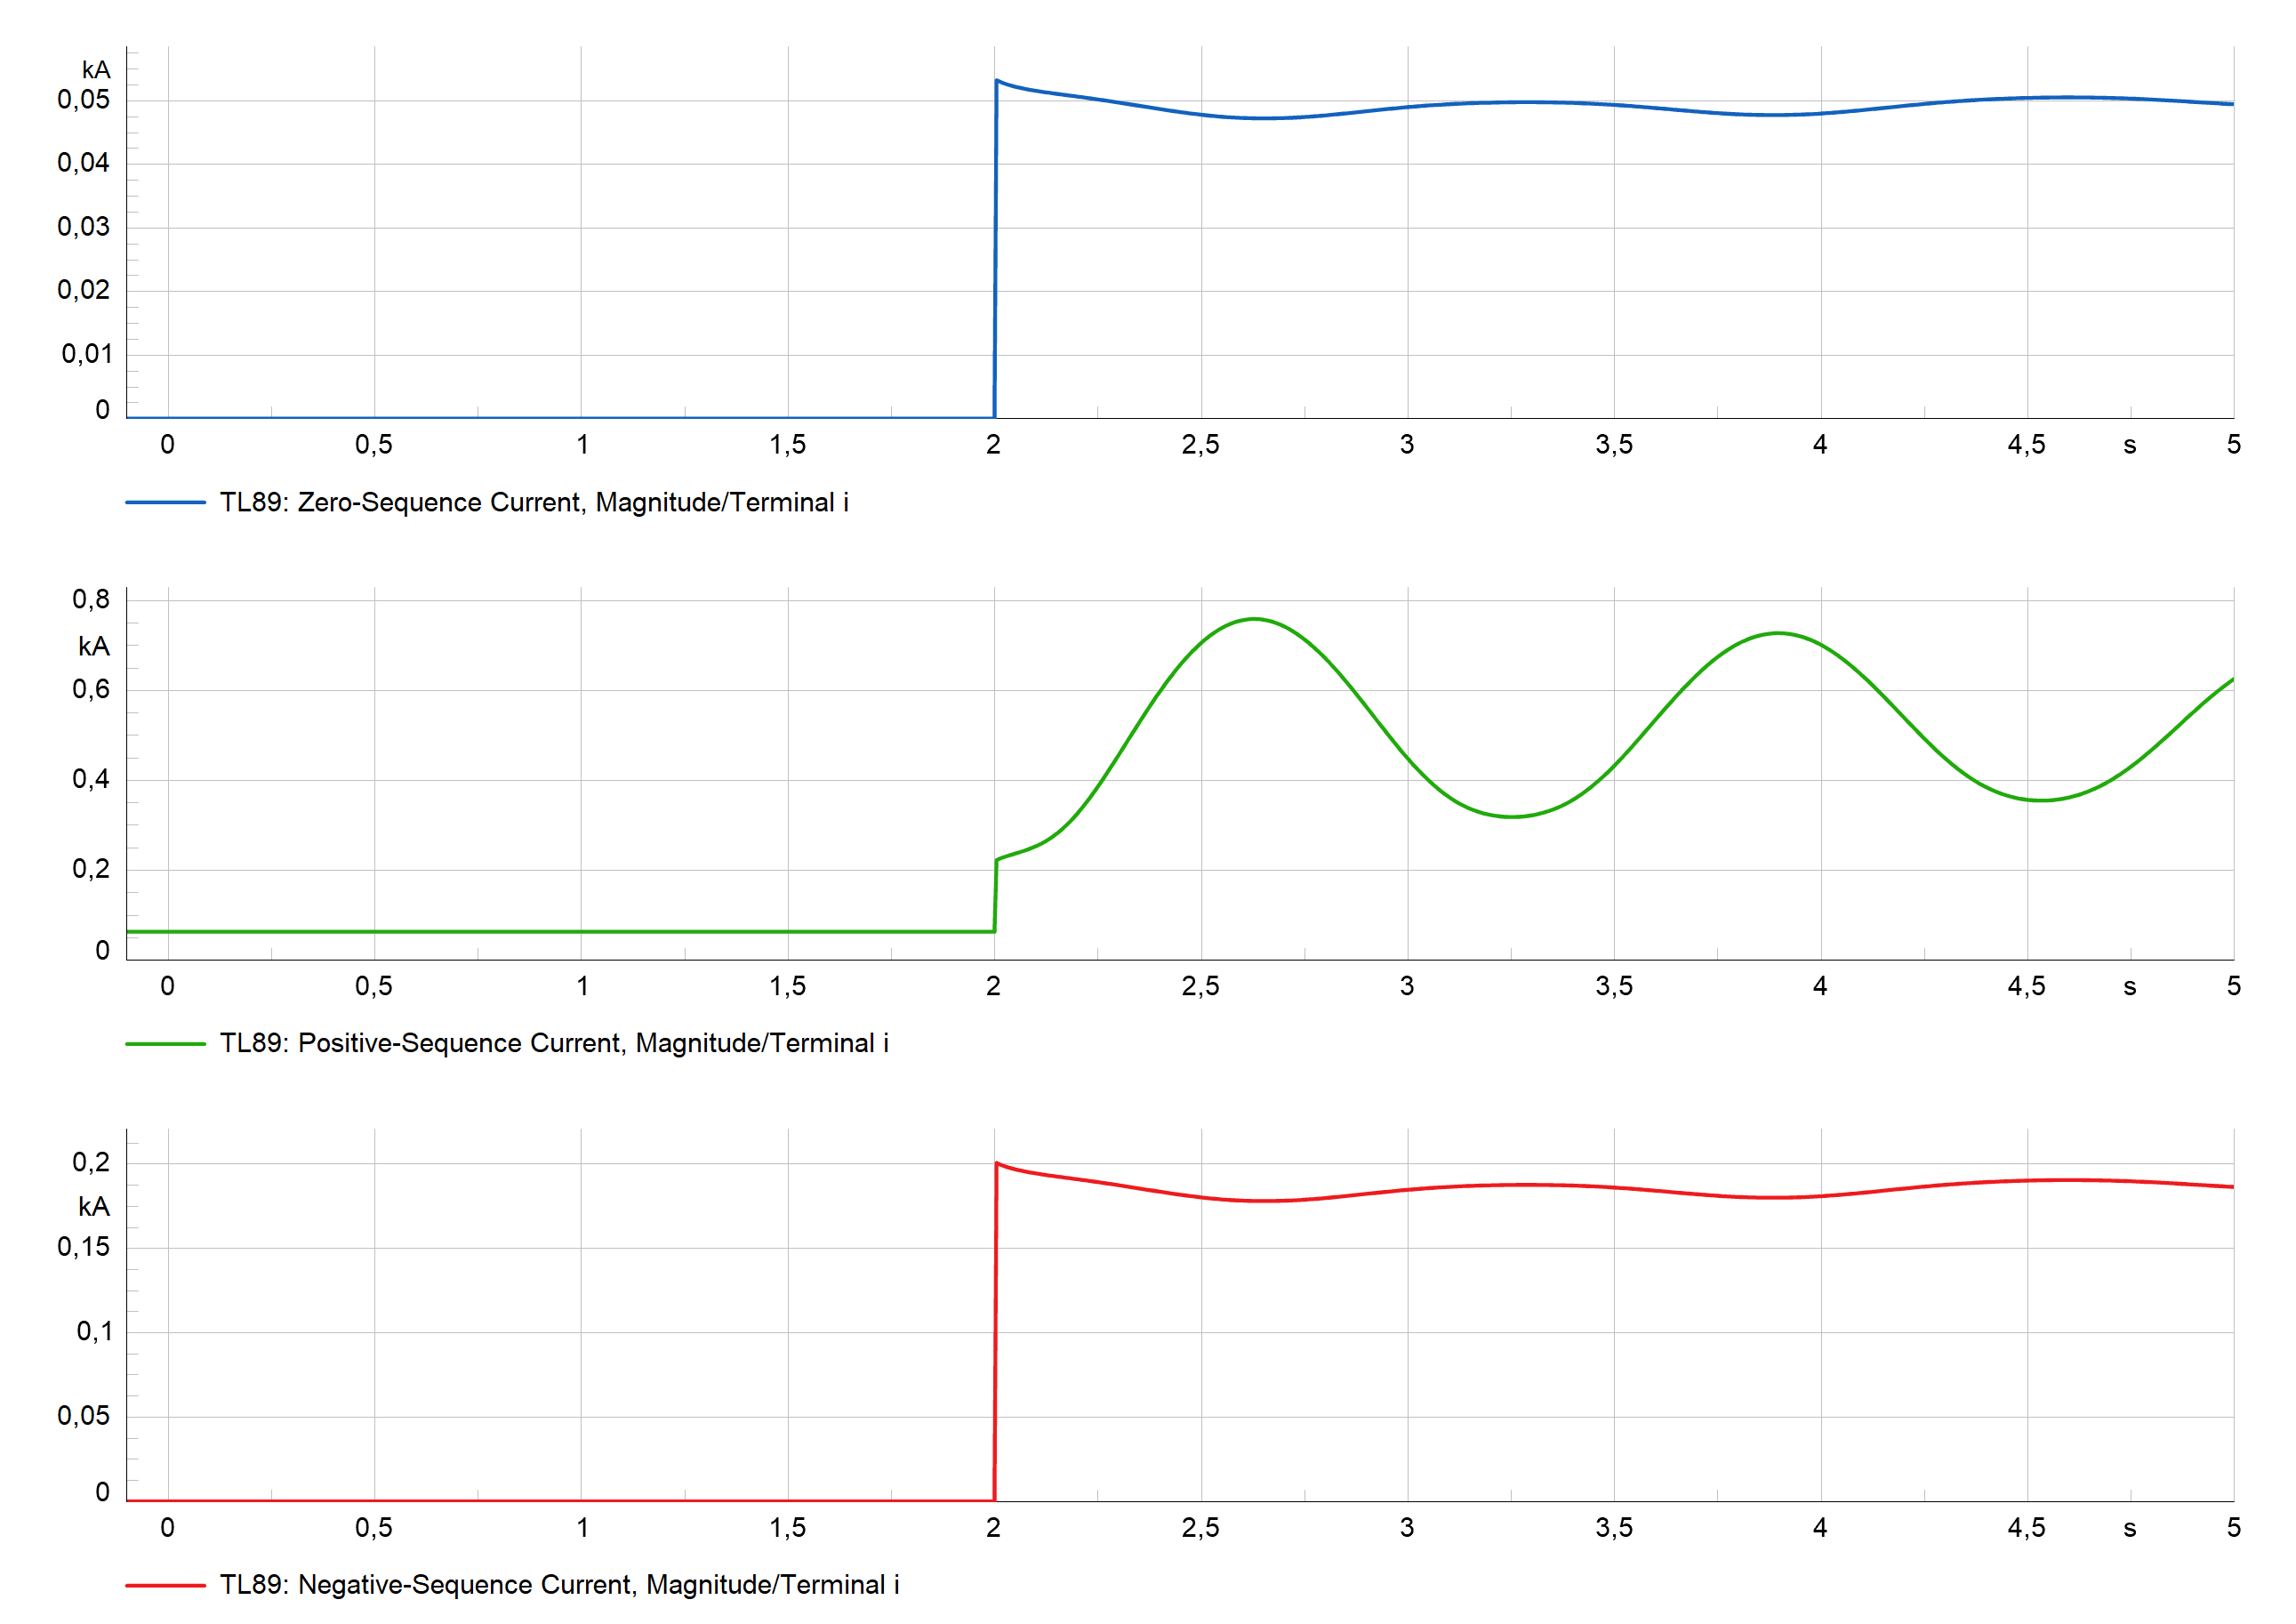
\includegraphics[width=0.8\textwidth]{contents/chapter-4/TL89_seq_external_slg.png}
    \caption{Dekomposisi Komponen Urutan Arus pada Gangguan External Single Line-to-Ground}
    \label{fig:TL89_seq_external_slg}
\end{figure}

Berdasarkan Gambar \ref{fig:TL89_seq_external_slg}, gangguan external \textit{single line-to-ground} menyebabkan peningkatan pada komponen arus urutan positif, negatif, dan nol. Komponen urutan positif naik dari 0,063 kA menjadi sekitar 0,225 kA sesaat setelah gangguan terjadi, kemudian berosilasi pada rentang 0,32 - 0,76 kA. Komponen urutan negatif meningkat dari 0 kA menjadi sekitar 0,2 kA dan berosilasi pada rentang 0,18 - 0,19 kA, sedangkan komponen urutan nol meningkat dari 0 kA menjadi sekitar 0,053 kA dan berosilasi pada rentang 0,048 - 0,05 kA.

Peningkatan ketiga komponen tersebut menunjukkan adanya ketidakseimbangan arus yang signifikan akibat gangguan. Komponen urutan positif meningkat karena adanya arus yang mengalir melalui jalur gangguan, sedangkan komponen urutan negatif dan nol meningkat akibat ketidakseimbangan arus pada gangguan satu fasa ke tanah. Dengan demikian, pola kenaikan komponen urutan pada Gambar \ref{fig:TL89_seq_external_slg} memperlihatkan karakteristik gangguan external \textit{single line-to-ground} pada saluran TL89.

\subsubsection{Gangguan External Double Line-to-Ground Fault}

Subbagian ini membahas perubahan komponen arus urutan pada saluran TL89 untuk kondisi sistem tanpa integrasi IBR saat terjadi gangguan external \textit{double line-to-ground}. Pembahasan difokuskan pada komponen urutan positif, negatif, dan nol, karena gangguan dua fasa ke tanah menghasilkan ketidakseimbangan arus yang tercermin pada ketiga komponen tersebut.

\begin{figure}[H]
    \centering
    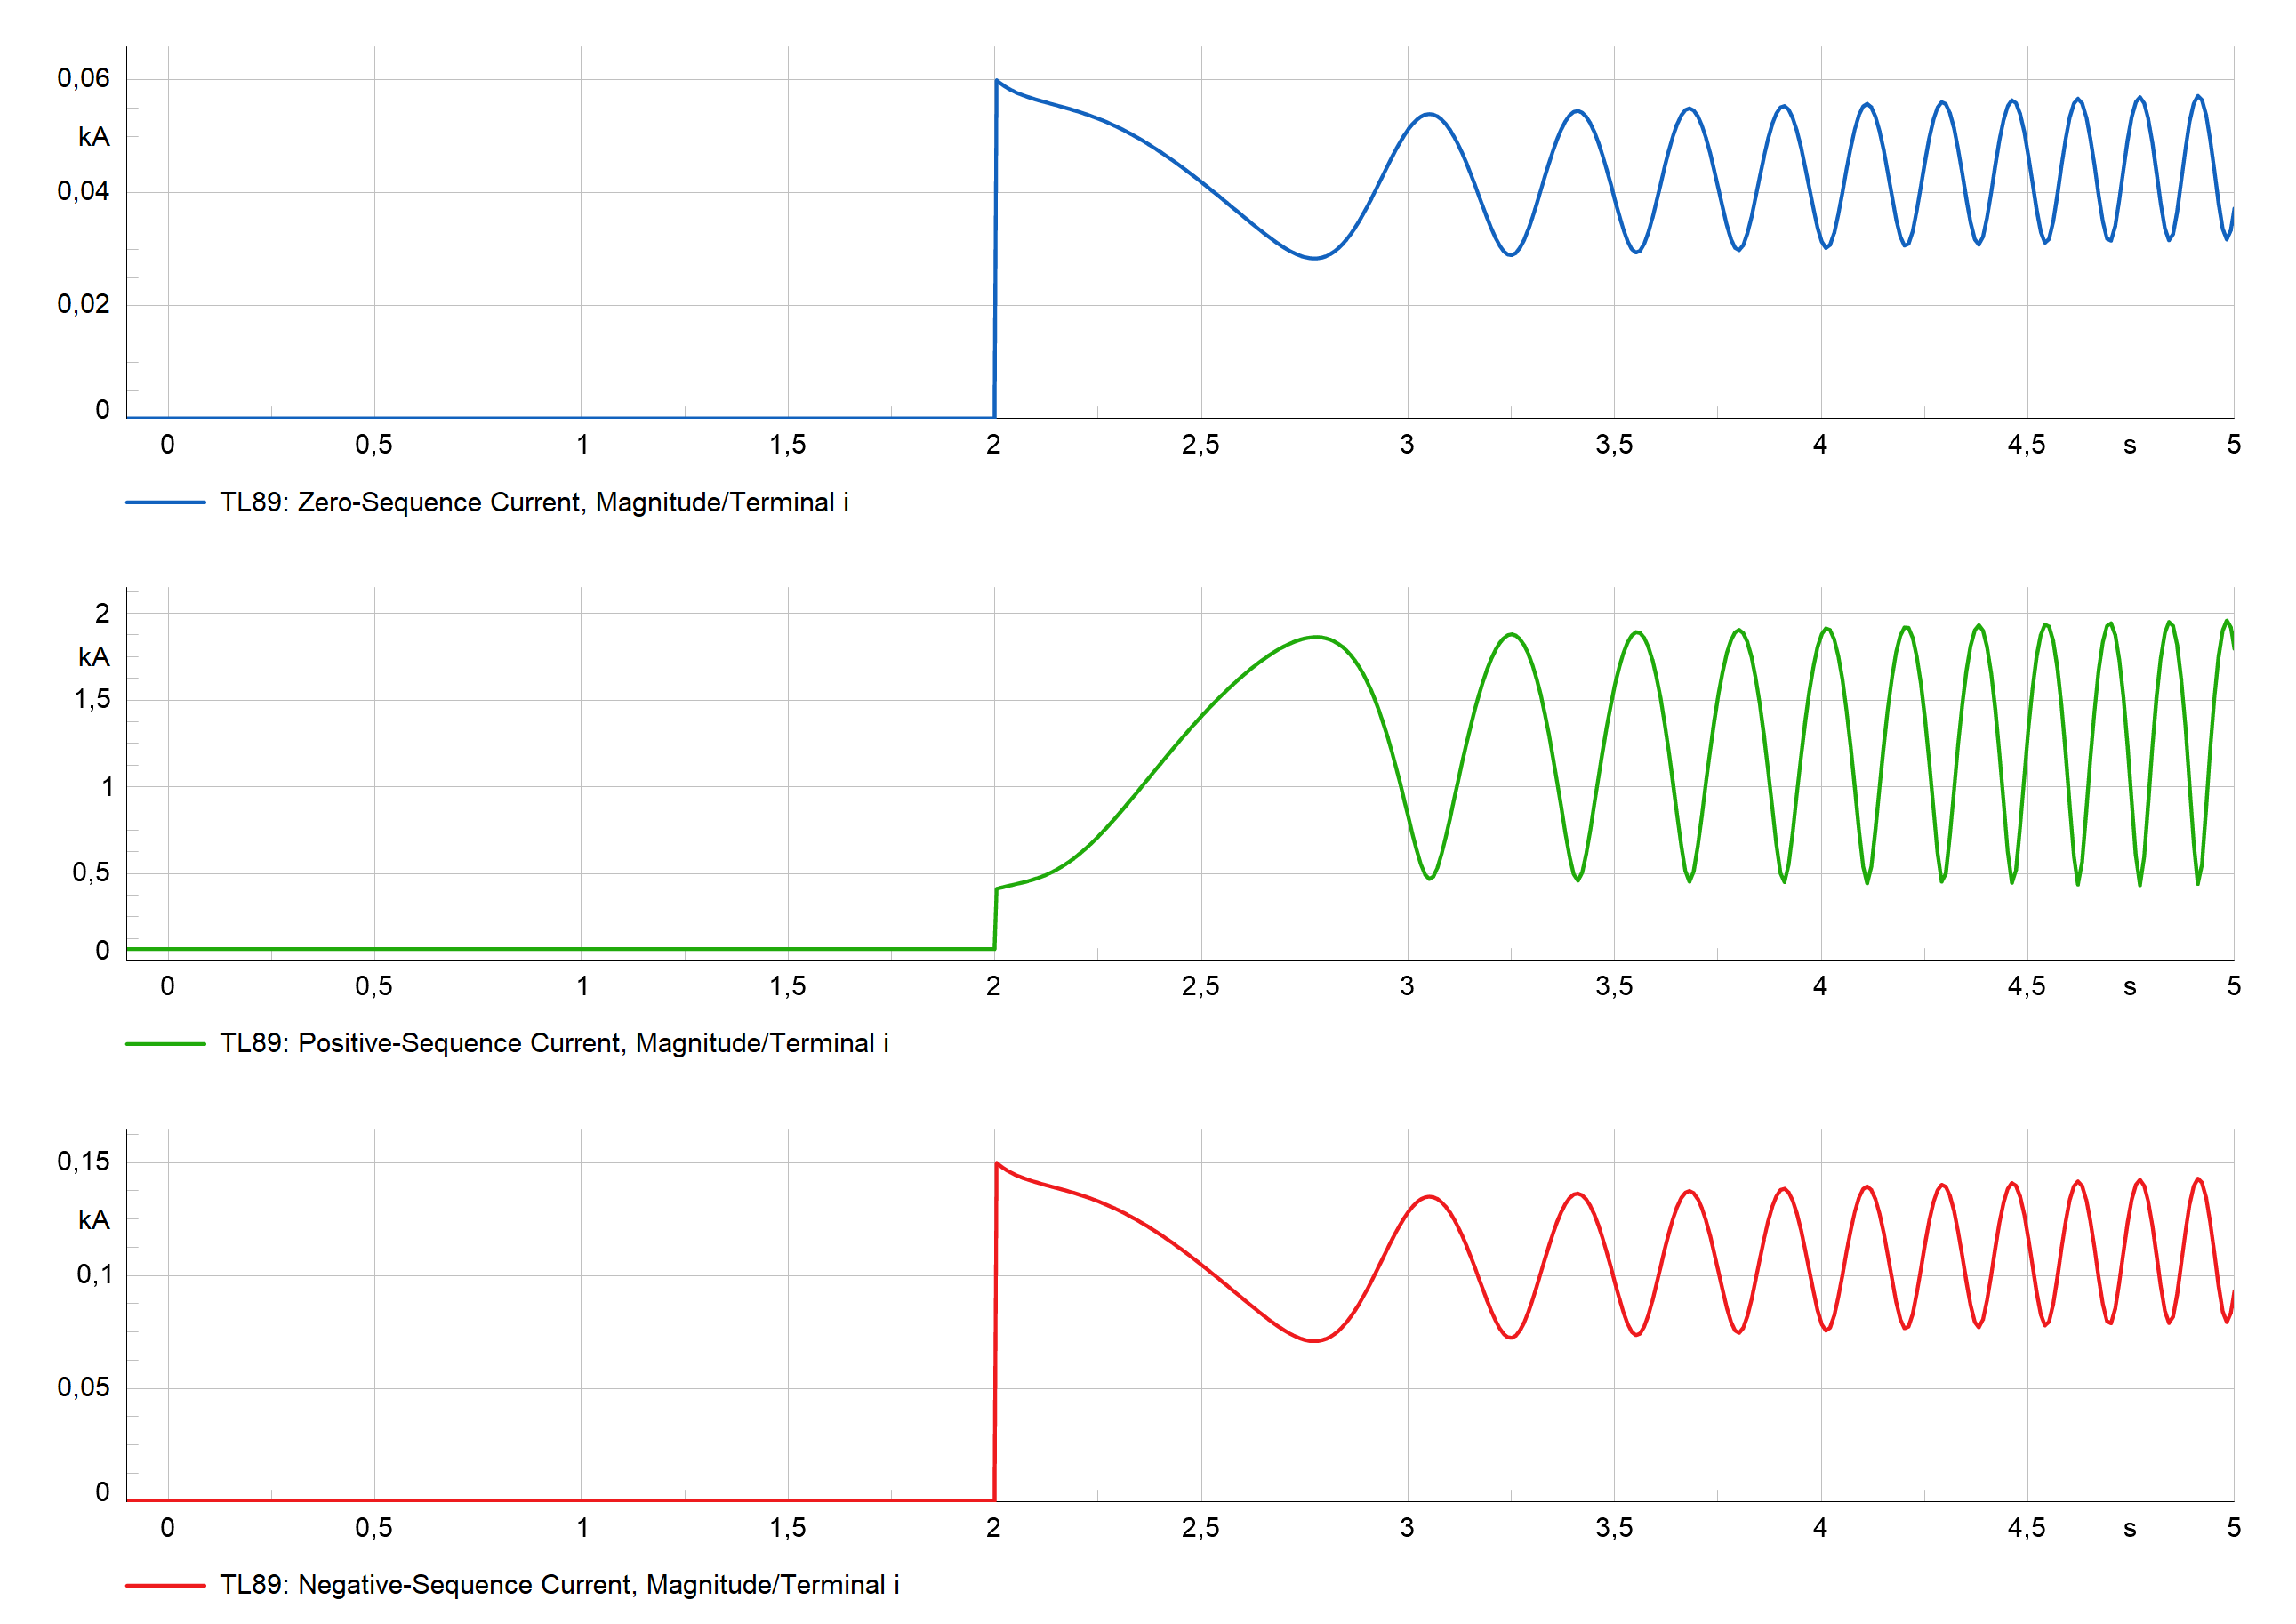
\includegraphics[width=0.8\textwidth]{contents/chapter-4/TL89_seq_external_dlg.png}
    \caption{Dekomposisi Komponen Urutan Arus pada Gangguan External Double Line-to-Ground}
    \label{fig:TL89_seq_external_dlg}
\end{figure}

Berdasarkan Gambar \ref{fig:TL89_seq_external_dlg}, gangguan external \textit{double line-to-ground} menyebabkan peningkatan pada komponen arus urutan positif, negatif, dan nol. Komponen urutan positif naik dari 0,063 kA menjadi sekitar 0,4112 kA sesaat setelah gangguan terjadi, kemudian berosilasi pada rentang 0,4313 - 1,95 kA. Komponen urutan negatif meningkat dari 0 kA menjadi sekitar 0,15 kA dan berosilasi pada rentang 0,079 - 0,14 kA, sedangkan komponen urutan nol meningkat dari 0 kA menjadi sekitar 0,06 kA dan berosilasi pada rentang 0,032 - 0,057 kA.

Peningkatan ketiga komponen tersebut menunjukkan adanya ketidakseimbangan arus yang signifikan akibat gangguan. Komponen urutan positif meningkat karena adanya arus yang mengalir melalui jalur gangguan, sedangkan komponen urutan negatif dan nol meningkat akibat ketidakseimbangan arus pada gangguan dua fasa ke tanah. Dengan demikian, pola pada Gambar \ref{fig:TL89_seq_external_dlg} memperlihatkan karakteristik gangguan external \textit{double line-to-ground} pada saluran TL89.

\subsection{Skenario 1: WT Type 3 Internal DLG Fault}

Subbagian ini membahas dekomposisi komponen urutan arus pada Skenario 1, yaitu kondisi integrasi WT Type 3 saat terjadi gangguan internal \textit{double line-to-ground}. Pembahasan difokuskan pada perubahan komponen urutan positif, negatif, dan nol yang terbaca selama gangguan, sehingga pola ketidakseimbangan arus pada skenario ini dapat diamati secara lebih jelas.

\begin{figure}[H]
    \centering

    % Gambar sebelah kiri
    \begin{subfigure}[t]{0.48\textwidth}
        \centering
        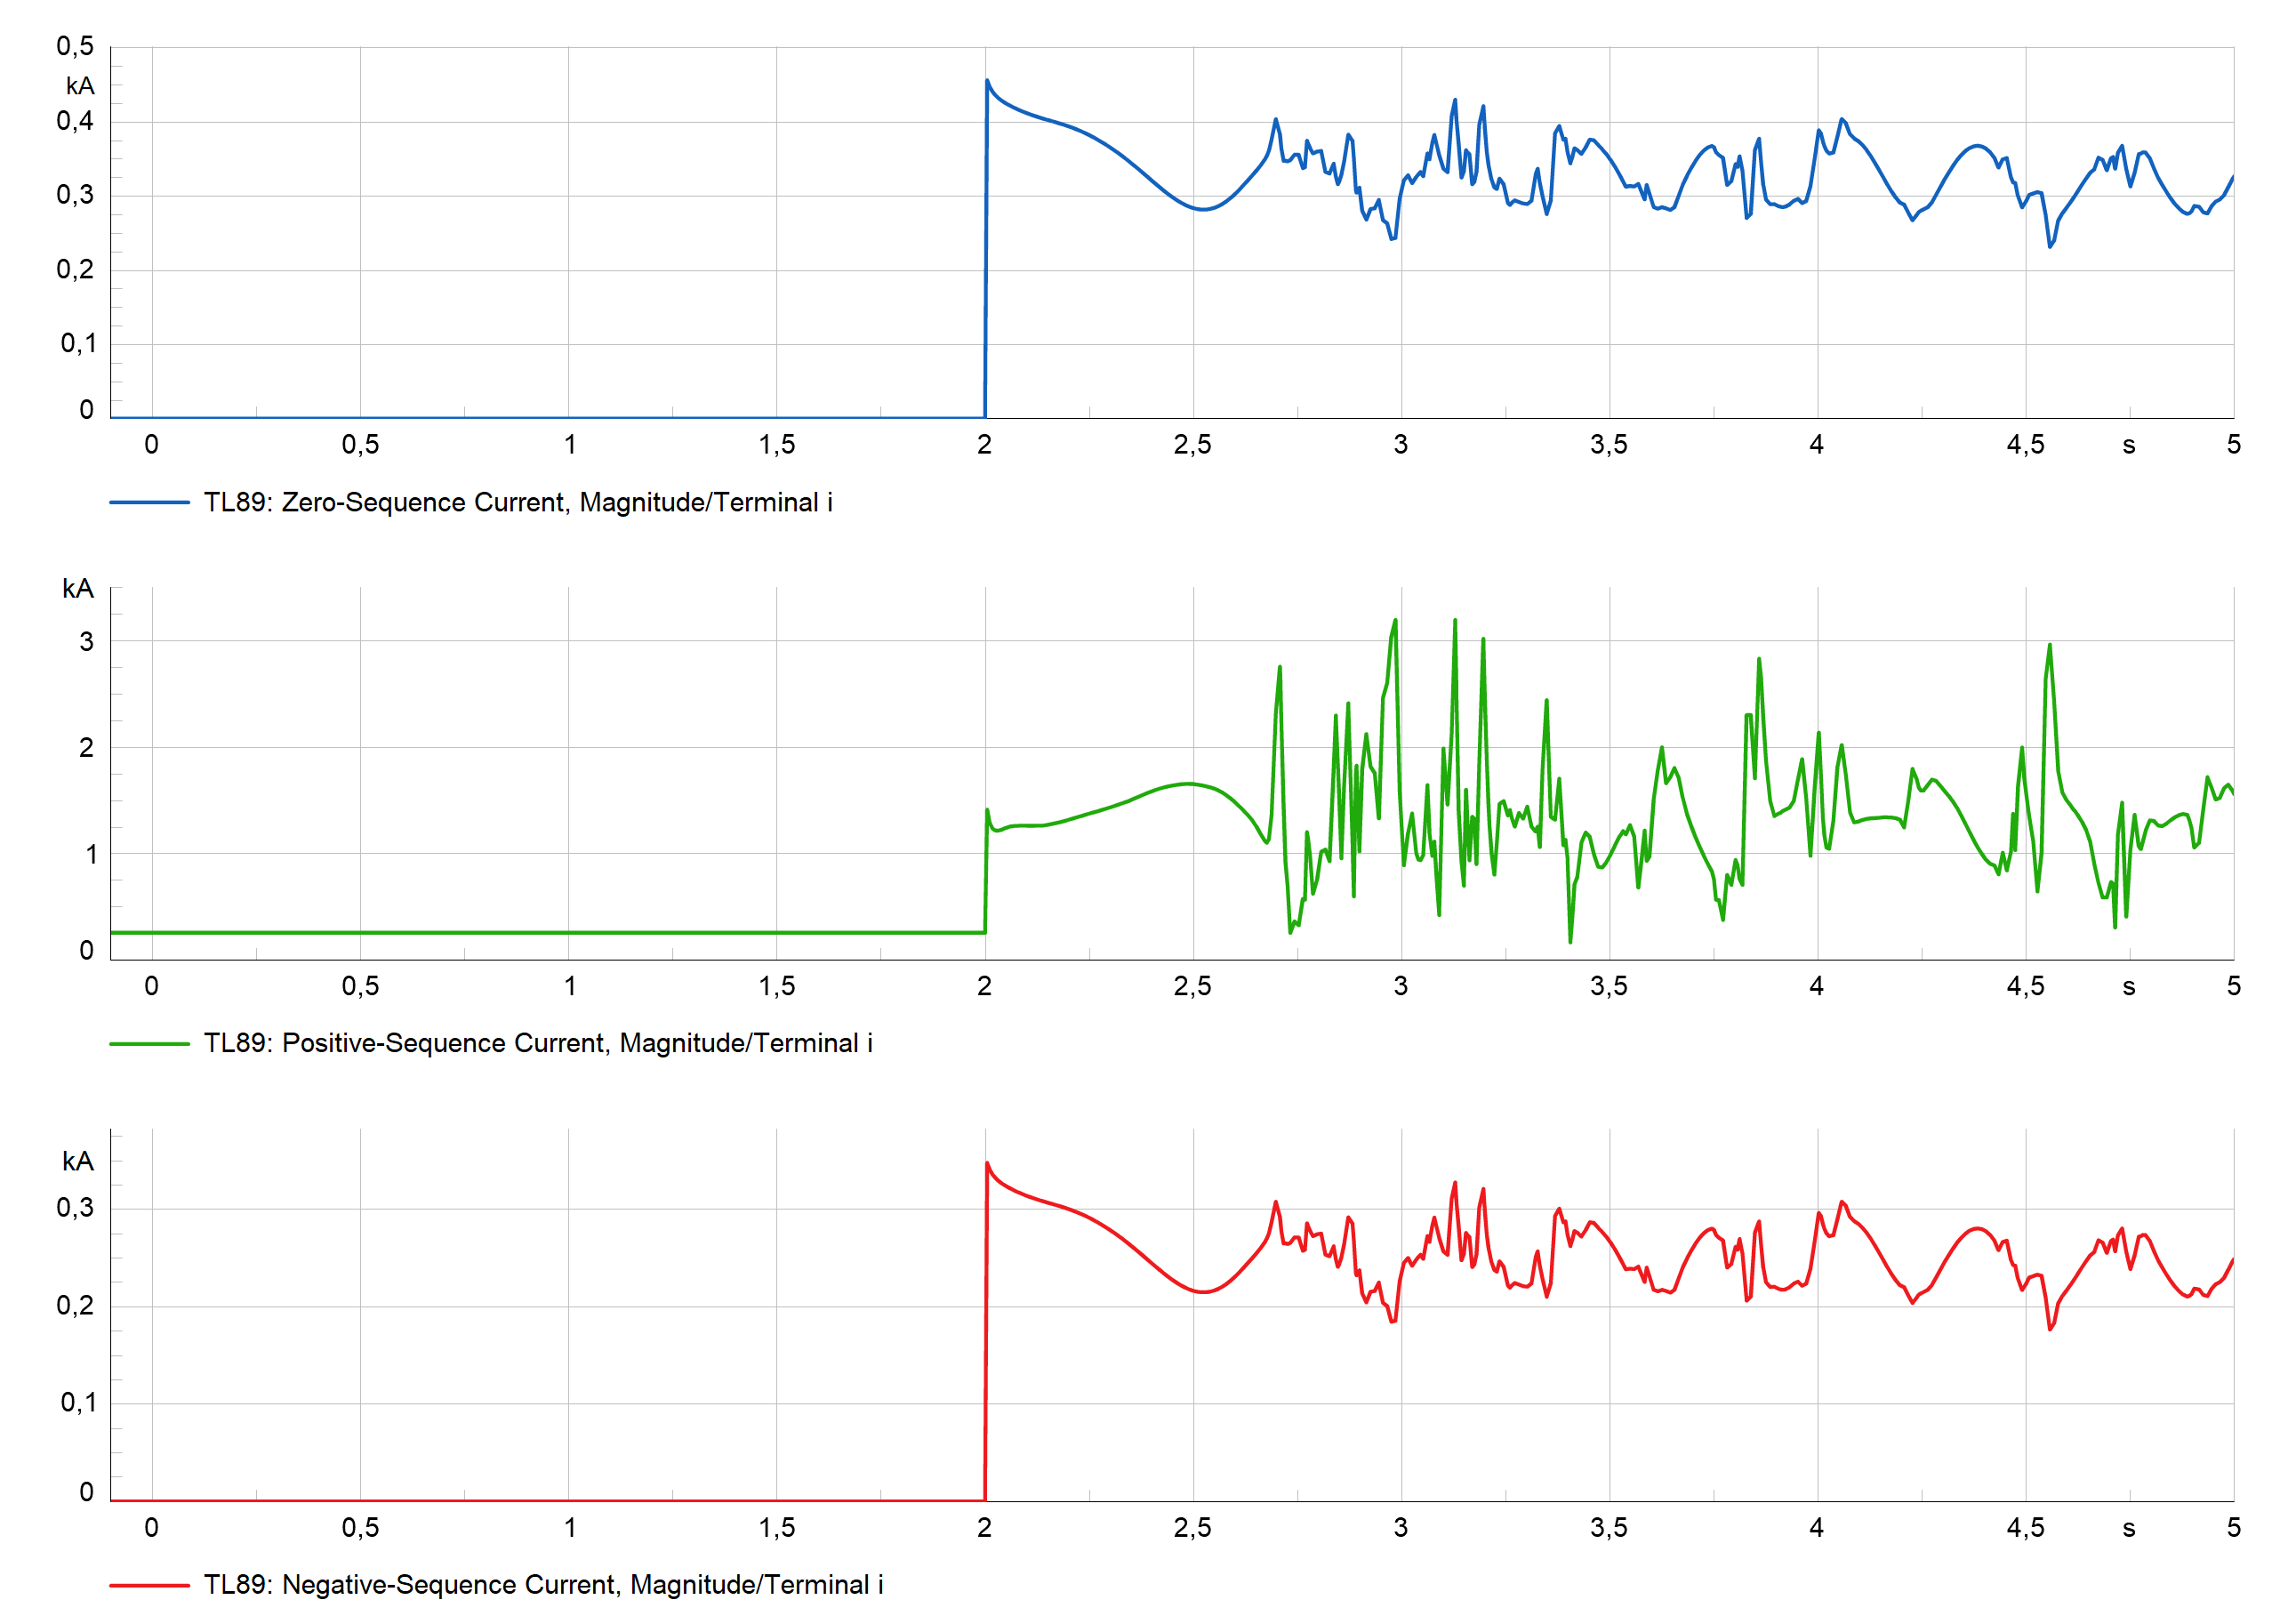
\includegraphics[width=\textwidth]{contents/chapter-4/TL89_seq_s1.png}
        \caption{Saluran TL89}
        \label{fig:sequence_current_tl89_s1}
    \end{subfigure}
    \hfill
    % Gambar sebelah kanan
    \begin{subfigure}[t]{0.48\textwidth}
        \centering
        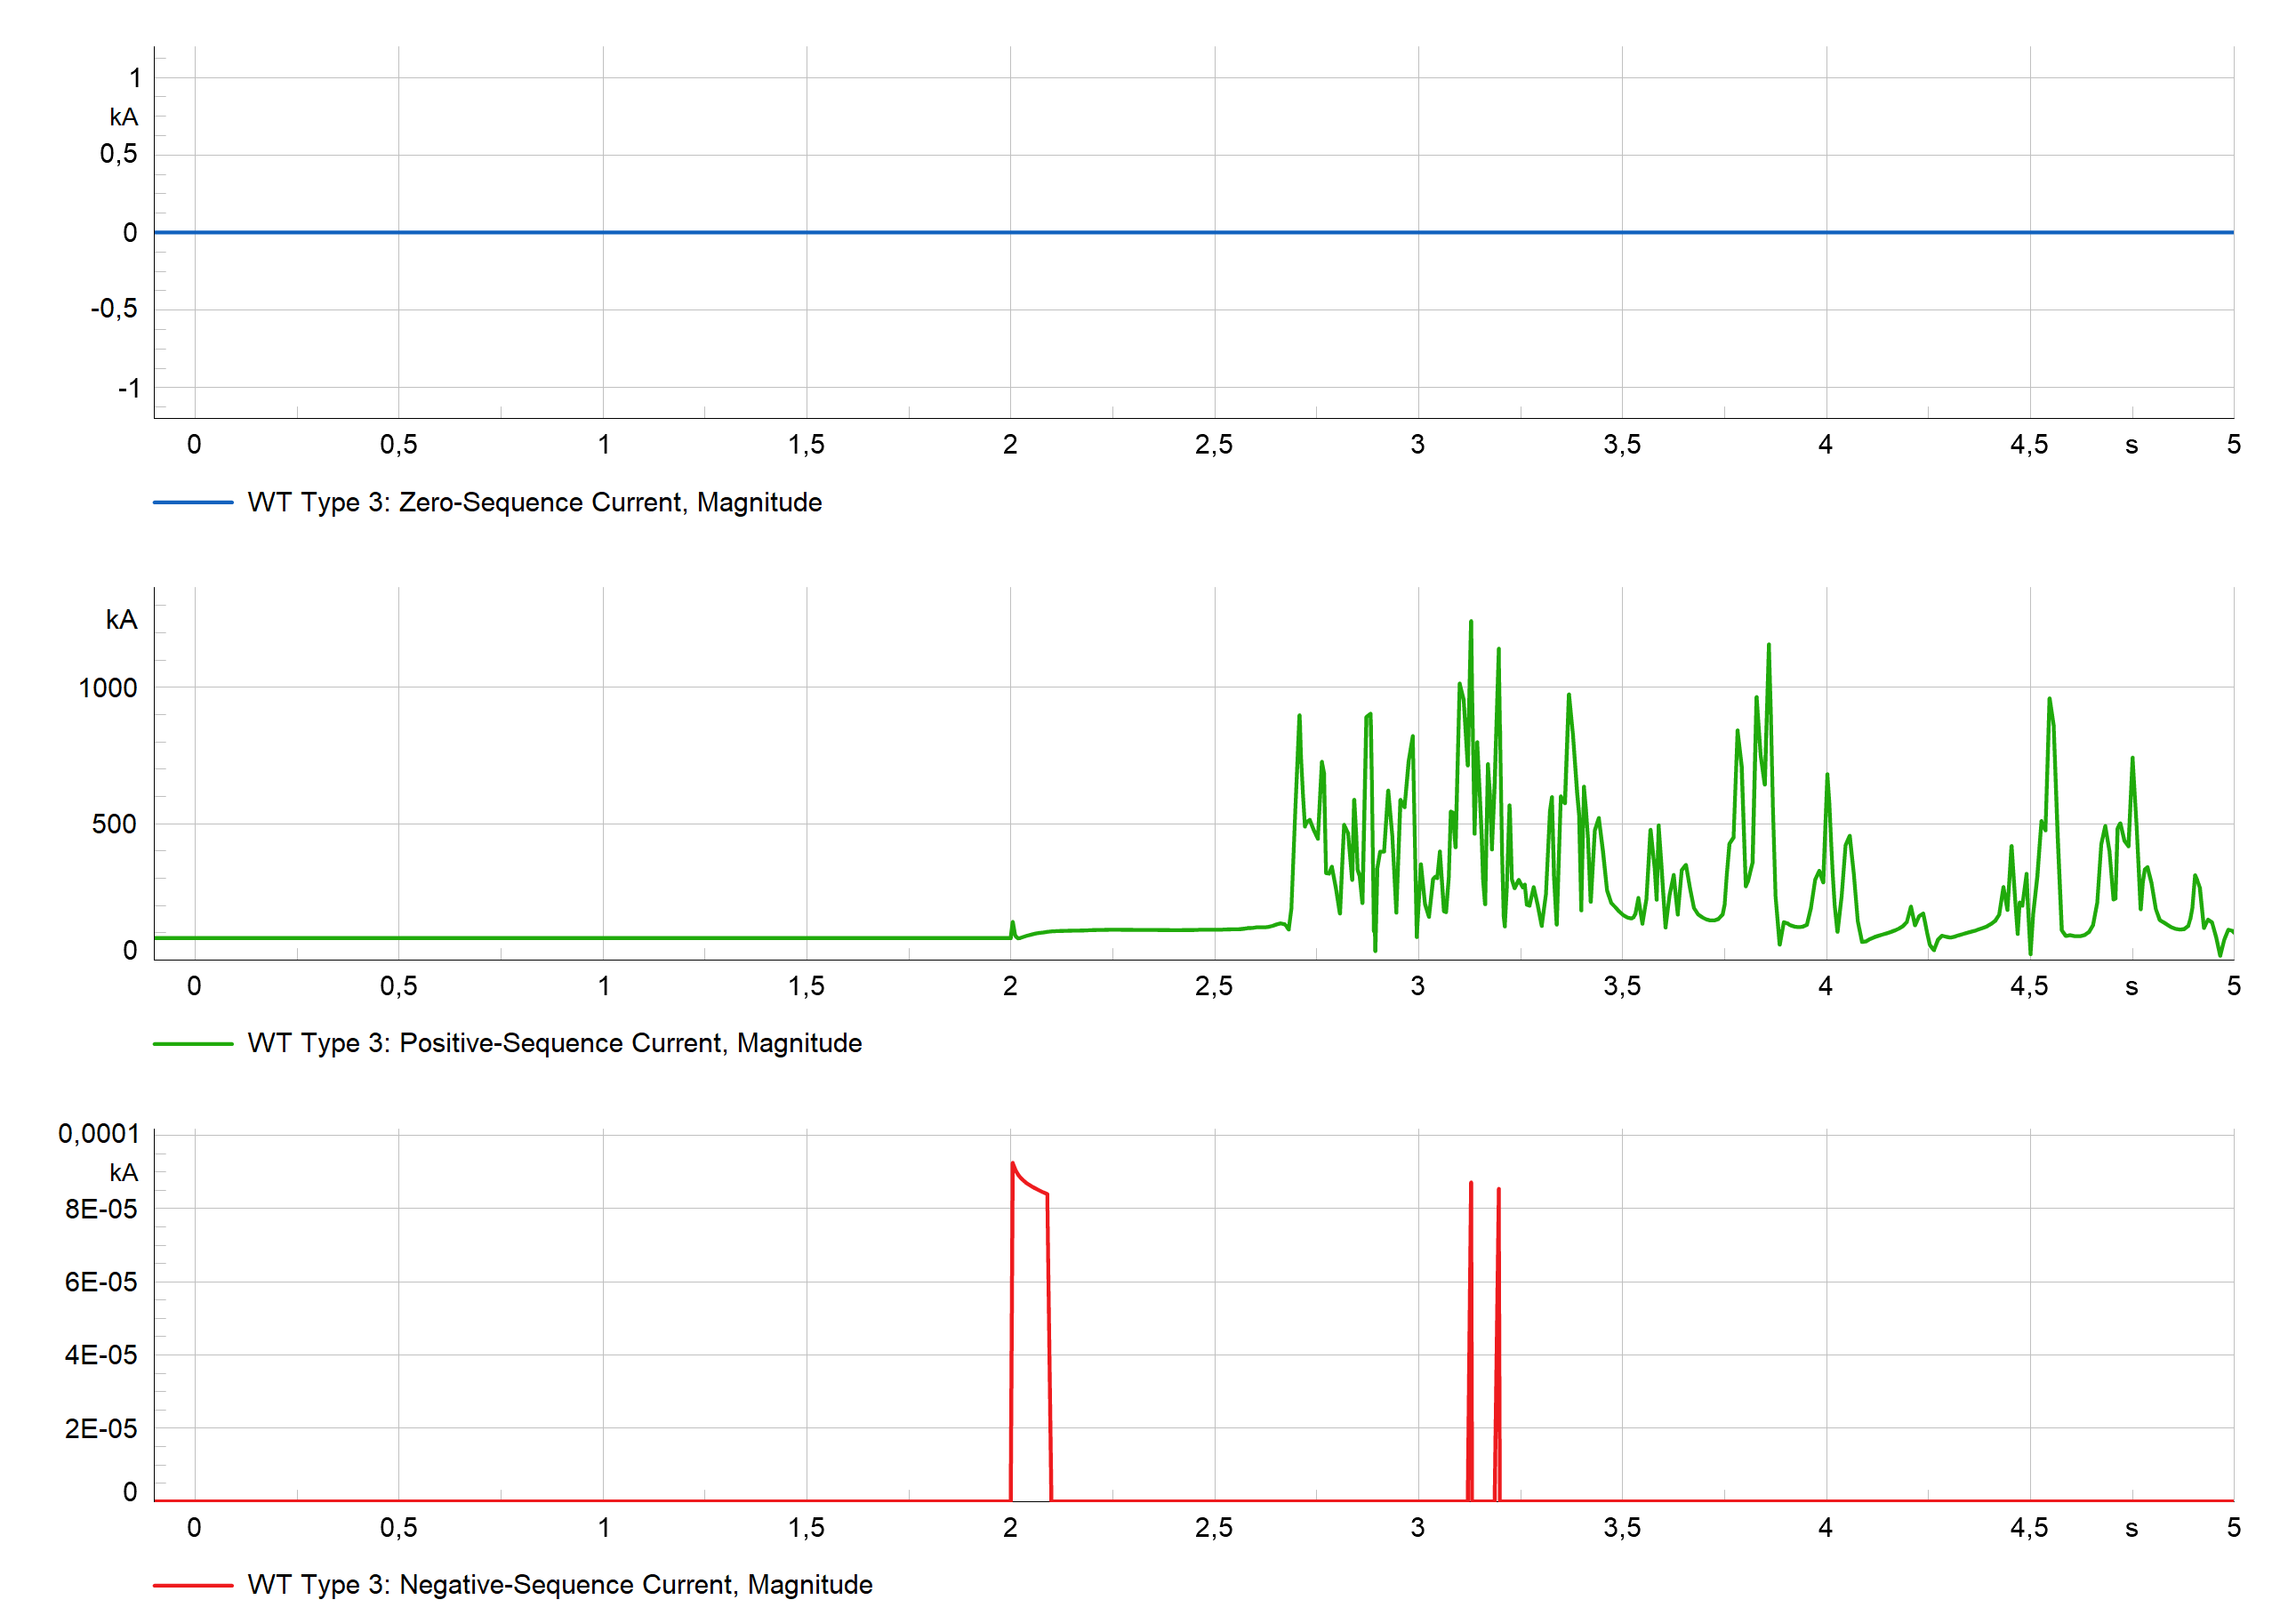
\includegraphics[width=\textwidth]{contents/chapter-4/WTT3_seq_internal_dlg.png}
        \caption{\textit{Wind Turbine Type 3}.}
        \label{fig:sequence_current_wtt3_s1}
    \end{subfigure}

    \caption{Dekomposisi Komponen Urutan Arus pada Skenario 1}
    \label{fig:decomposition_sequence_current_s1}
\end{figure}

Berdasarkan Gambar \ref{fig:decomposition_sequence_current_s1}, gangguan internal \textit{double line-to-ground} menyebabkan peningkatan pada komponen arus urutan positif, negatif, dan nol. Komponen urutan positif naik dari 0,2563 kA menjadi sekitar 1,414 kA sesaat setelah gangguan terjadi, kemudian berosilasi pada rentang 0,2554 - 3,198 kA. Komponen urutan negatif meningkat dari 0 kA menjadi sekitar 0,3478 kA dan berosilasi pada rentang 0,1765 - 0,3277 kA, sedangkan komponen urutan nol meningkat dari 0 kA menjadi sekitar 0,4563 kA dan berosilasi pada rentang 0,2315 - 0,4038 kA.

Peningkatan ketiga komponen tersebut menunjukkan adanya ketidakseimbangan arus yang signifikan akibat gangguan. Komponen urutan positif meningkat karena adanya arus yang mengalir melalui jalur gangguan, sedangkan komponen urutan negatif dan nol meningkat akibat ketidakseimbangan arus pada gangguan dua fasa ke tanah. Dengan demikian, pola pada Gambar \ref{fig:decomposition_sequence_current_s1} memperlihatkan karakteristik gangguan internal \textit{double line-to-ground} pada saluran TL89 untuk Skenario 1.

\subsection{Skenario 2: WT Type 4 External DLG Fault}

Subbagian ini membahas dekomposisi komponen urutan arus pada Skenario 2, yaitu kondisi sistem dengan integrasi WT Type 4 saat terjadi gangguan external \textit{double line-to-ground}. Pembahasan difokuskan pada perubahan komponen urutan positif, negatif, dan nol yang terbaca pada saluran TL89 serta sisi WT Type 4, karena gangguan dua fasa ke tanah menimbulkan ketidakseimbangan arus yang dapat diamati melalui ketiga komponen tersebut.

\begin{figure}[H]
    \centering

    % Gambar sebelah kiri
    \begin{subfigure}[t]{0.48\textwidth}
        \centering
        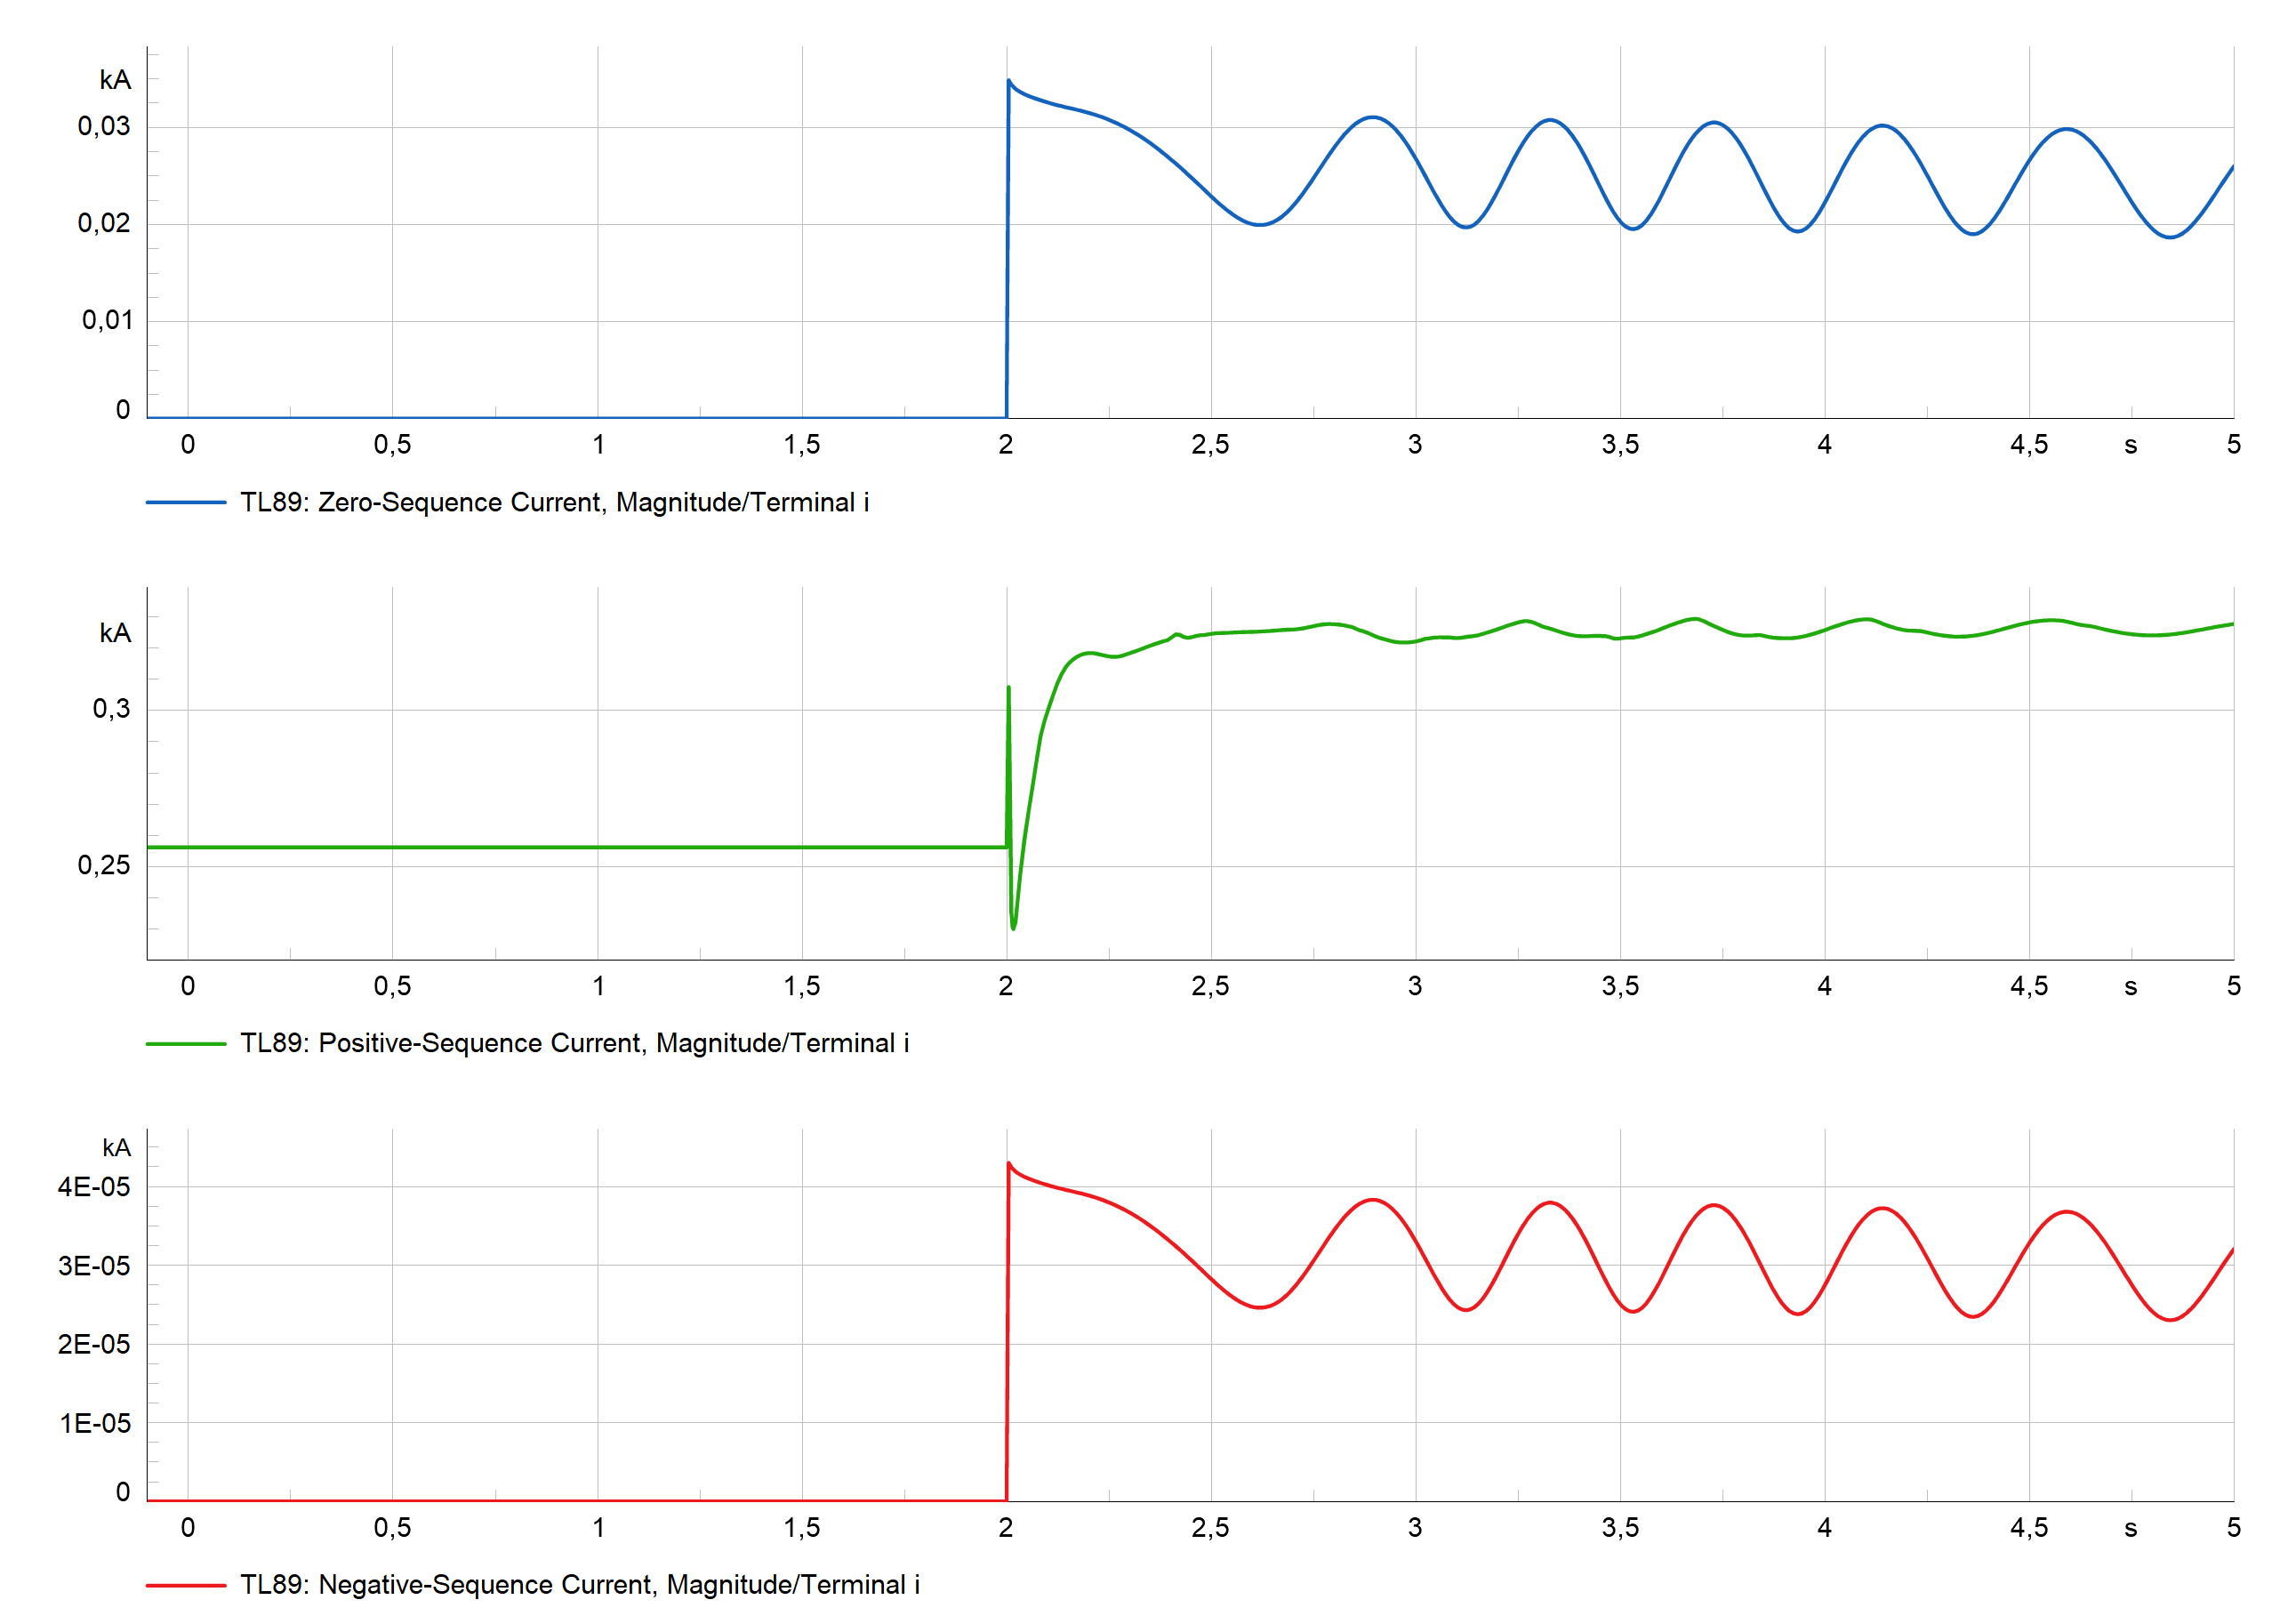
\includegraphics[width=\textwidth]{contents/chapter-4/TL89_seq_s2.png}
        \caption{Saluran TL89}
        \label{fig:sequence_current_tl89_s2}
    \end{subfigure}
    \hfill
    % Gambar sebelah kanan
    \begin{subfigure}[t]{0.48\textwidth}
        \centering
        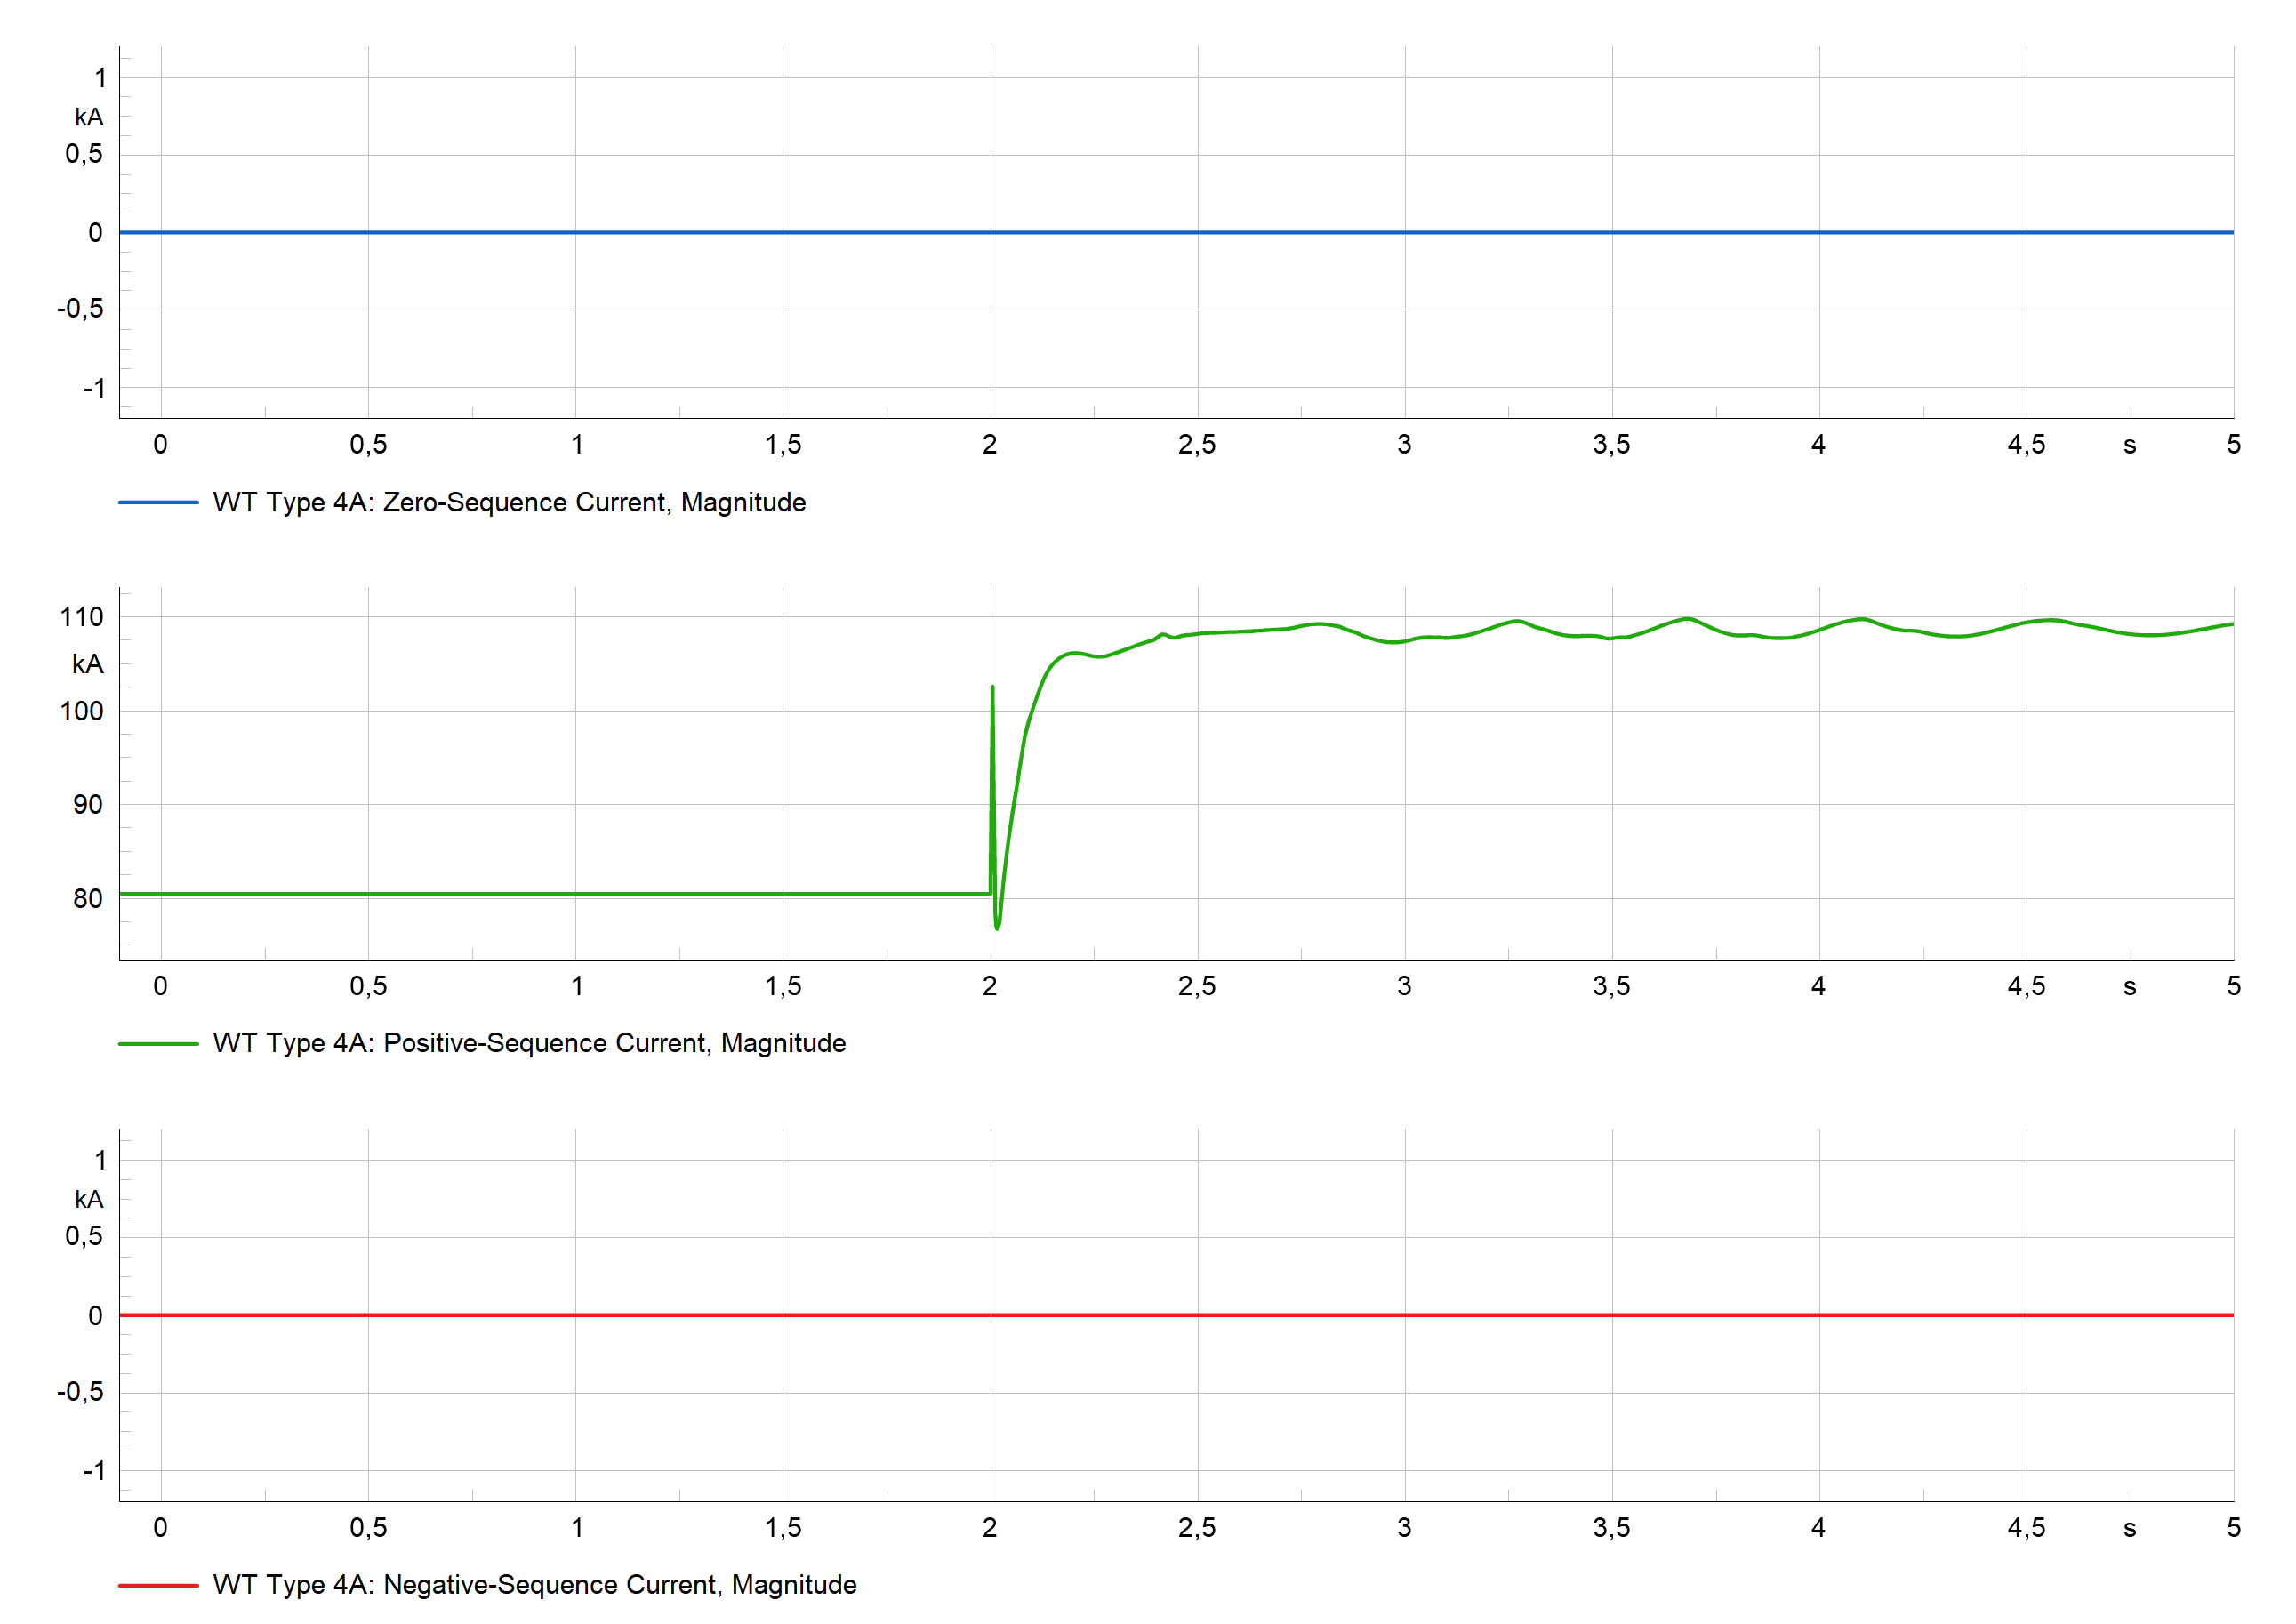
\includegraphics[width=\textwidth]{contents/chapter-4/WTT4_seq_external_dlg.png}
        \caption{\textit{Wind Turbine Type 4}.}
        \label{fig:sequence_current_wtt4_s2}
    \end{subfigure}

    \caption{Dekomposisi Komponen Urutan Arus pada Skenario 2}
    \label{fig:decomposition_sequence_current_s2}
\end{figure}

Berdasarkan Gambar \ref{fig:decomposition_sequence_current_s2}, gangguan external \textit{double line-to-ground} menyebabkan kenaikan pada komponen arus urutan positif, negatif, dan nol. Komponen urutan positif naik dari 0,2563 kA menjadi sekitar 0,31 kA sesaat setelah gangguan terjadi, kemudian berosilasi pada rentang 0,324 - 0,329 kA. Komponen urutan negatif meningkat dari 0 kA menjadi sekitar 0,000043 kA dan berosilasi pada rentang 0,000023 - 0,000037 kA. Sementara itu, komponen urutan nol meningkat dari 0 kA menjadi sekitar 0,035 kA dan berosilasi pada rentang 0,019 - 0,03 kA.

Kenaikan ketiga komponen tersebut menunjukkan adanya ketidakseimbangan arus akibat gangguan. Komponen urutan positif meningkat karena adanya arus yang mengalir melalui jalur gangguan, sedangkan komponen urutan negatif dan nol muncul akibat ketidakseimbangan arus pada gangguan dua fasa ke tanah. Dengan demikian, pola pada Gambar \ref{fig:decomposition_sequence_current_s2} memperlihatkan karakteristik gangguan external \textit{double line-to-ground} pada saluran TL89 untuk Skenario 2.

\subsection{Skenario 3: WT Type 3 External DLG Fault}

\begin{figure}[H]
    \centering

    % Gambar sebelah kiri
    \begin{subfigure}[t]{0.48\textwidth}
        \centering
        \includegraphics[width=\textwidth]{contents/chapter-4/tl89_seq_s3.png}
        \caption{Saluran TL89}
        \label{fig:sequence_current_tl89_s3}
    \end{subfigure}
    \hfill
    % Gambar sebelah kanan
    \begin{subfigure}[t]{0.48\textwidth}
        \centering
        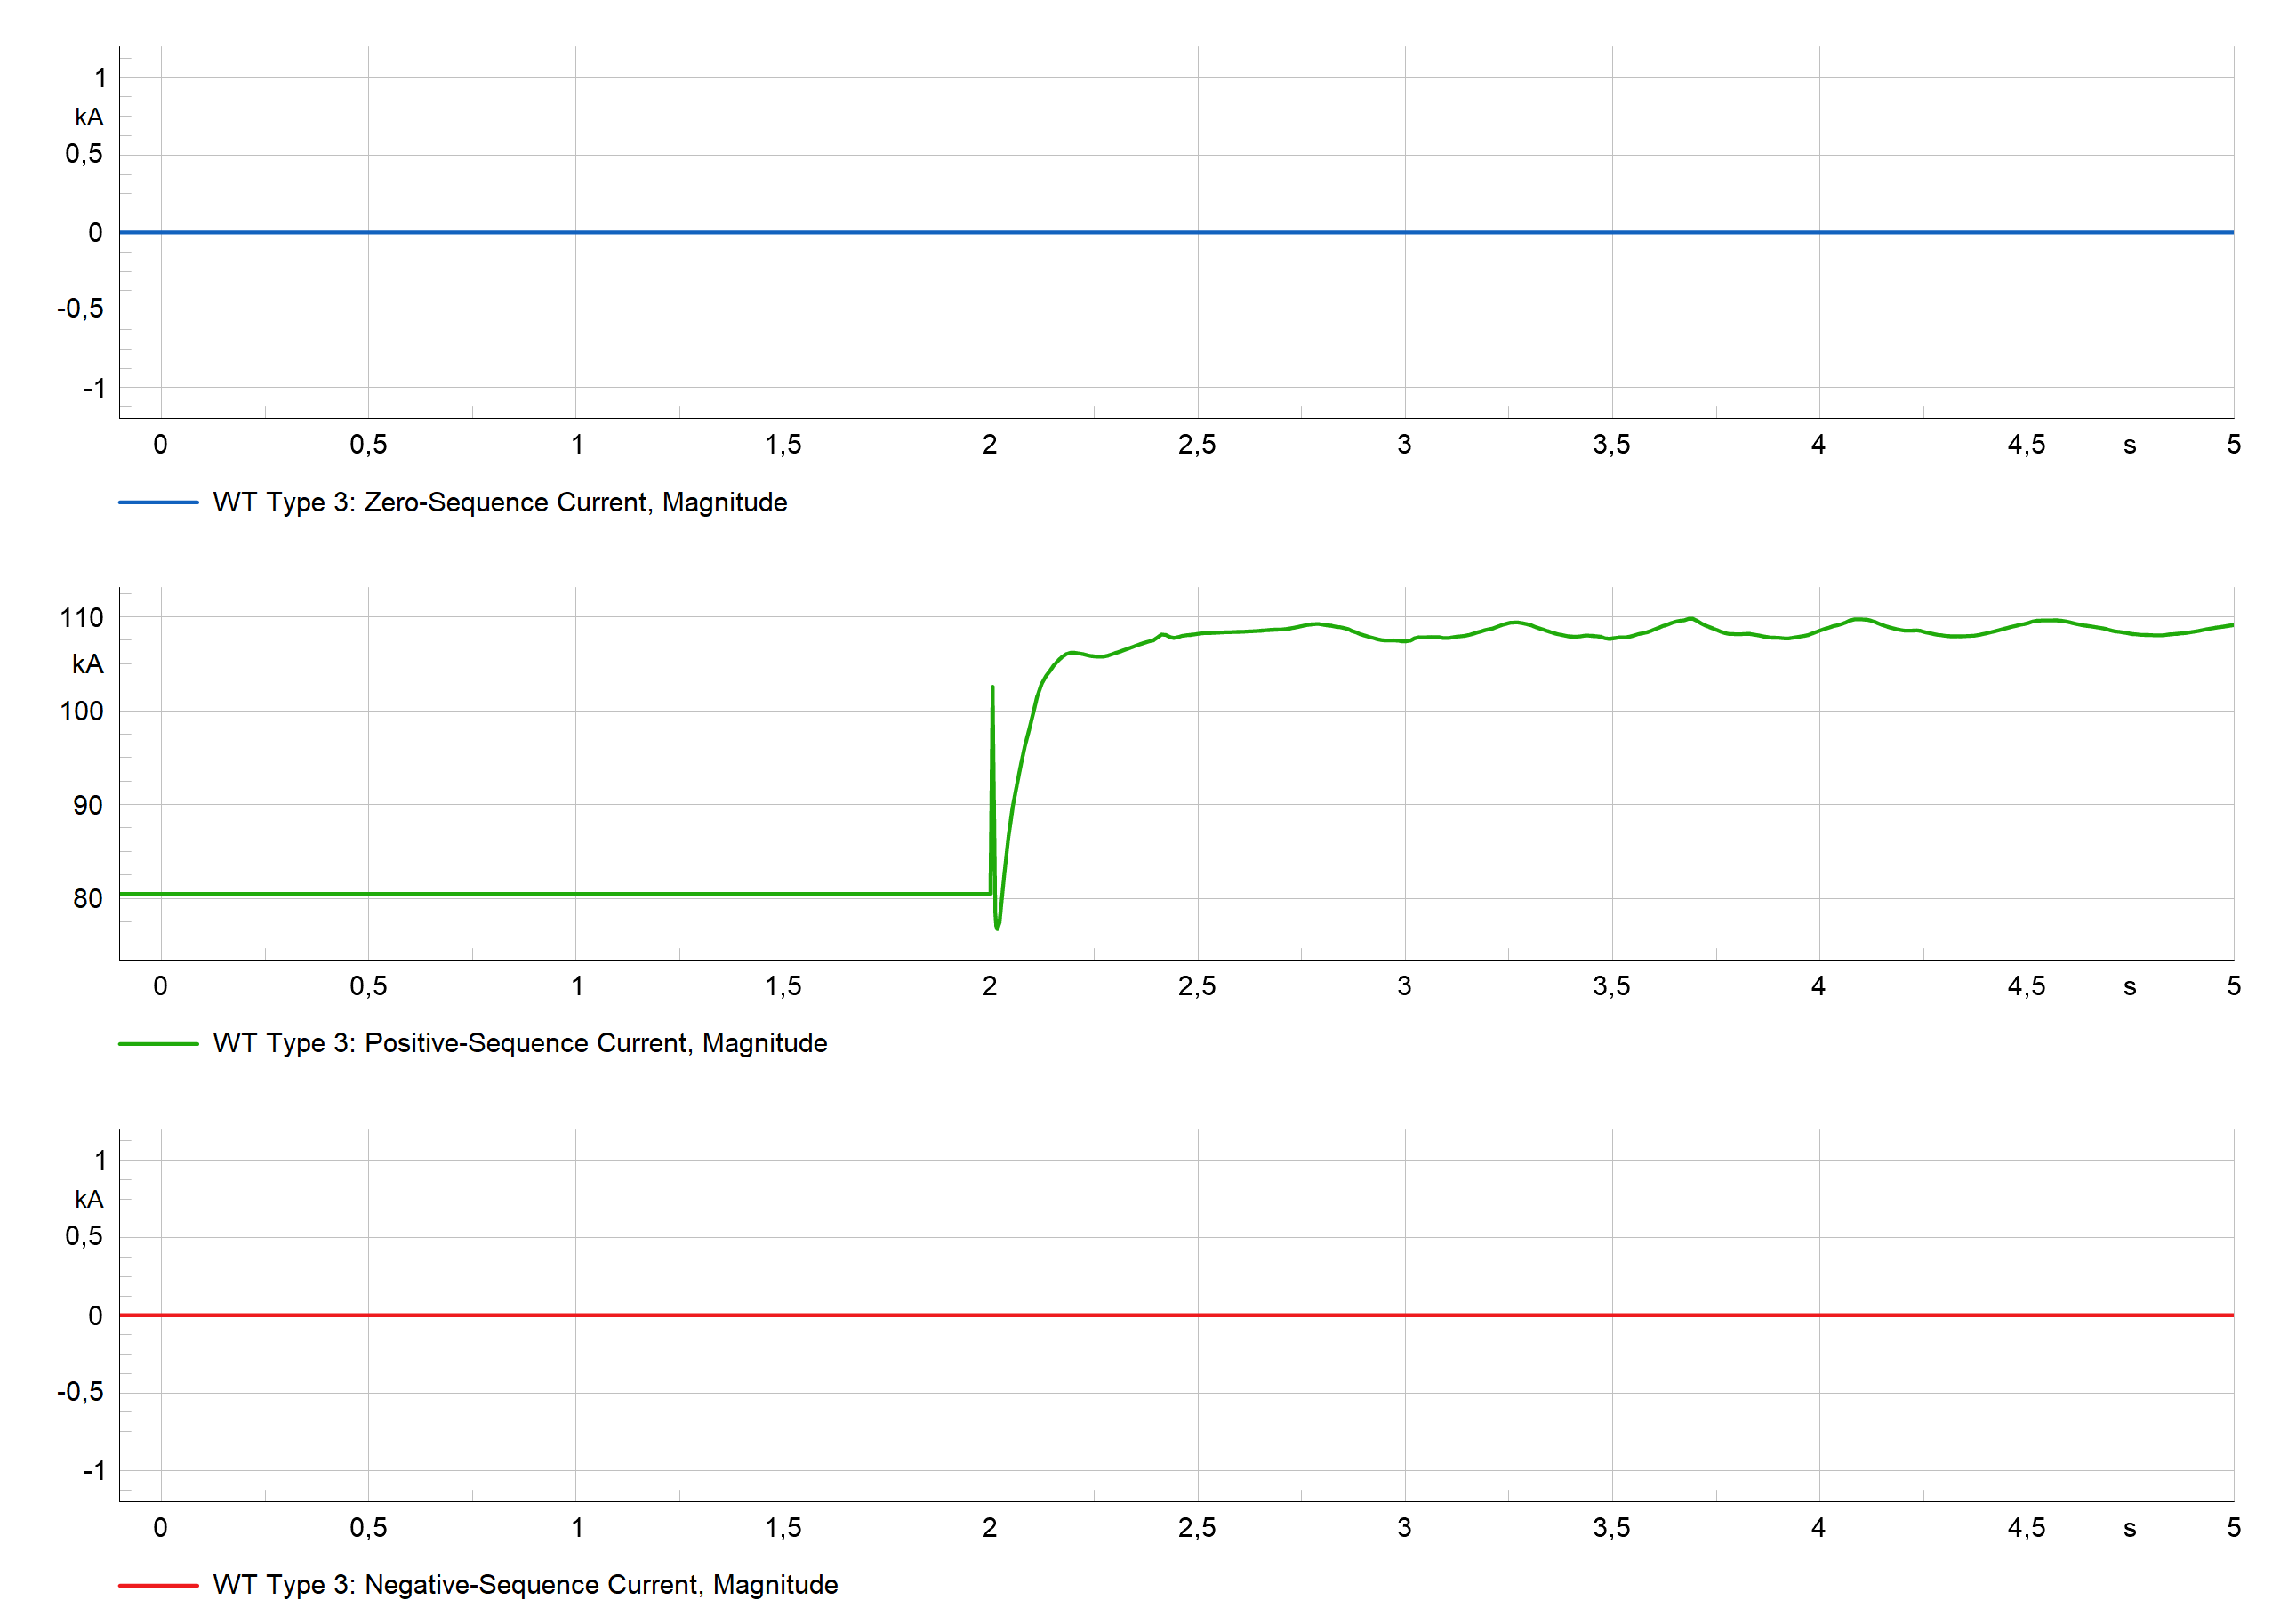
\includegraphics[width=\textwidth]{contents/chapter-4/WTT3_seq_external_dlg.png}
        \caption{\textit{Wind Turbine Type 3}.}
        \label{fig:sequence_current_wtt3_s3}
    \end{subfigure}

    \caption{Dekomposisi Komponen Urutan Arus pada Skenario 3}
    \label{fig:decomposition_sequence_current_s3}
\end{figure}

\subsection{Skenario 4: WT Type 3 External 3P Fault}

\begin{figure}[H]
    \centering

    % Gambar sebelah kiri
    \begin{subfigure}[t]{0.48\textwidth}
        \centering
        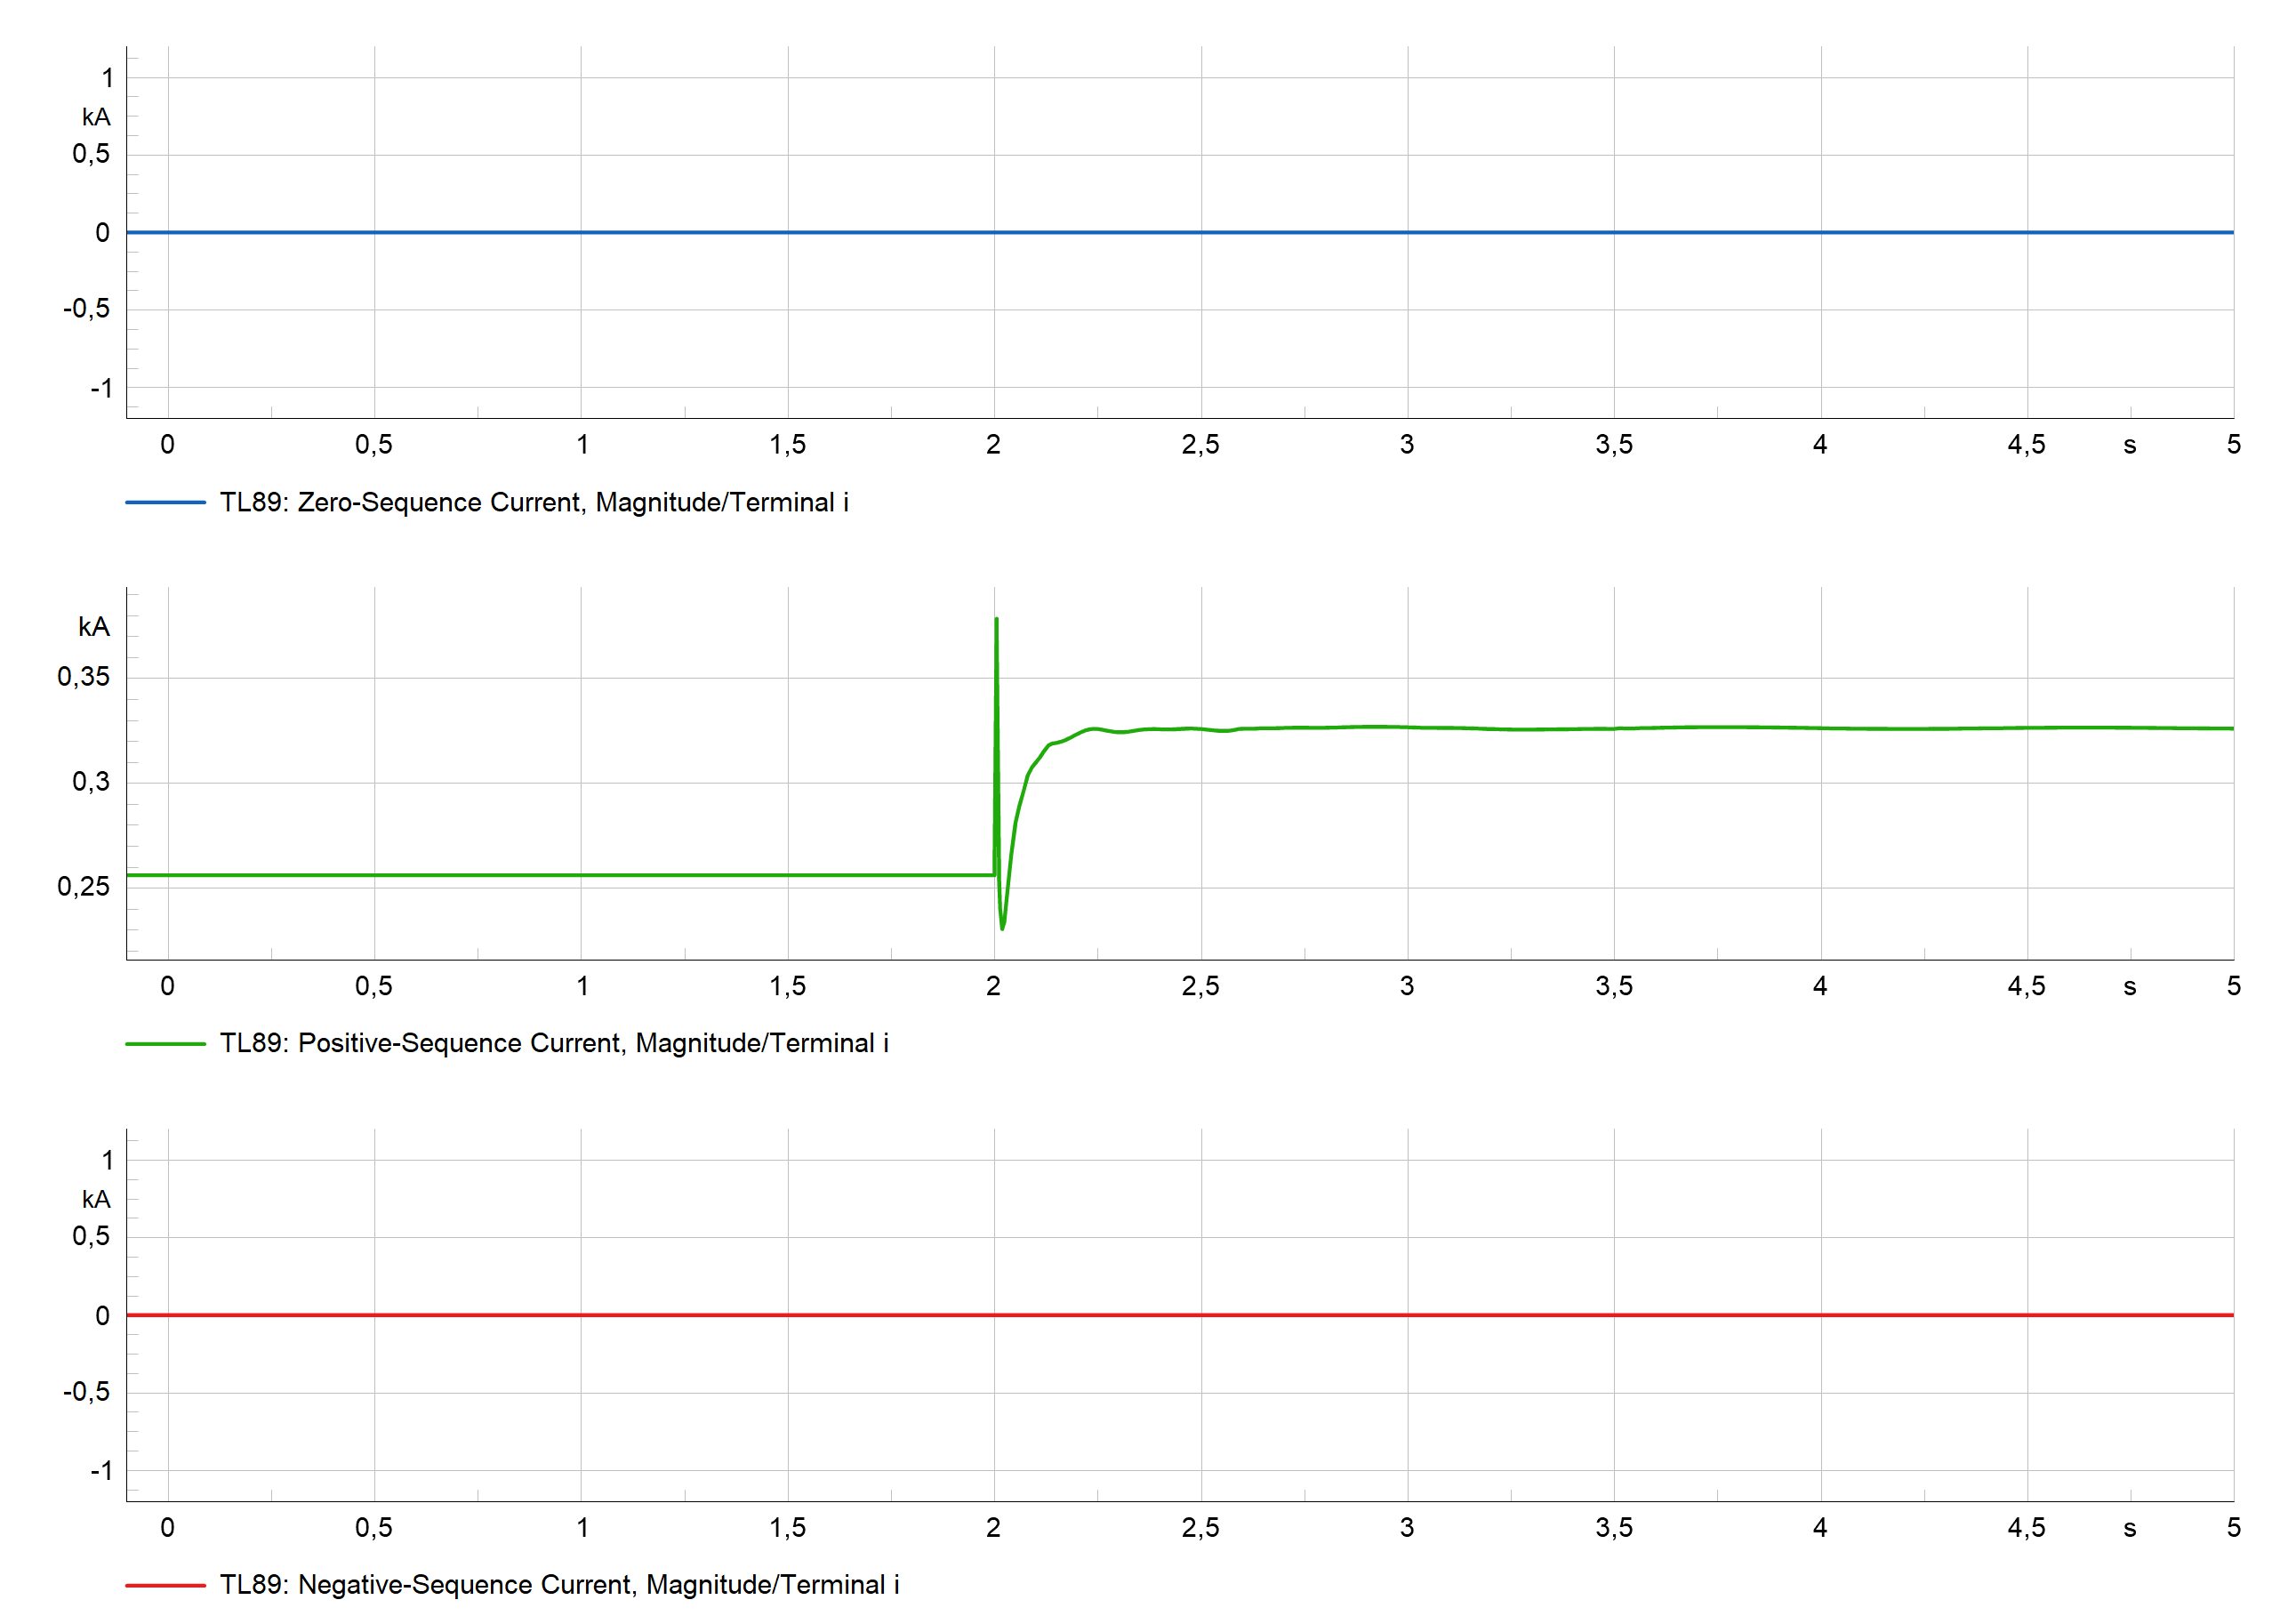
\includegraphics[width=\textwidth]{contents/chapter-4/TL89_seq_s4.png}
        \caption{Saluran TL89}
        \label{fig:sequence_current_tl89_s4}
    \end{subfigure}
    \hfill
    % Gambar sebelah kanan
    \begin{subfigure}[t]{0.48\textwidth}
        \centering
        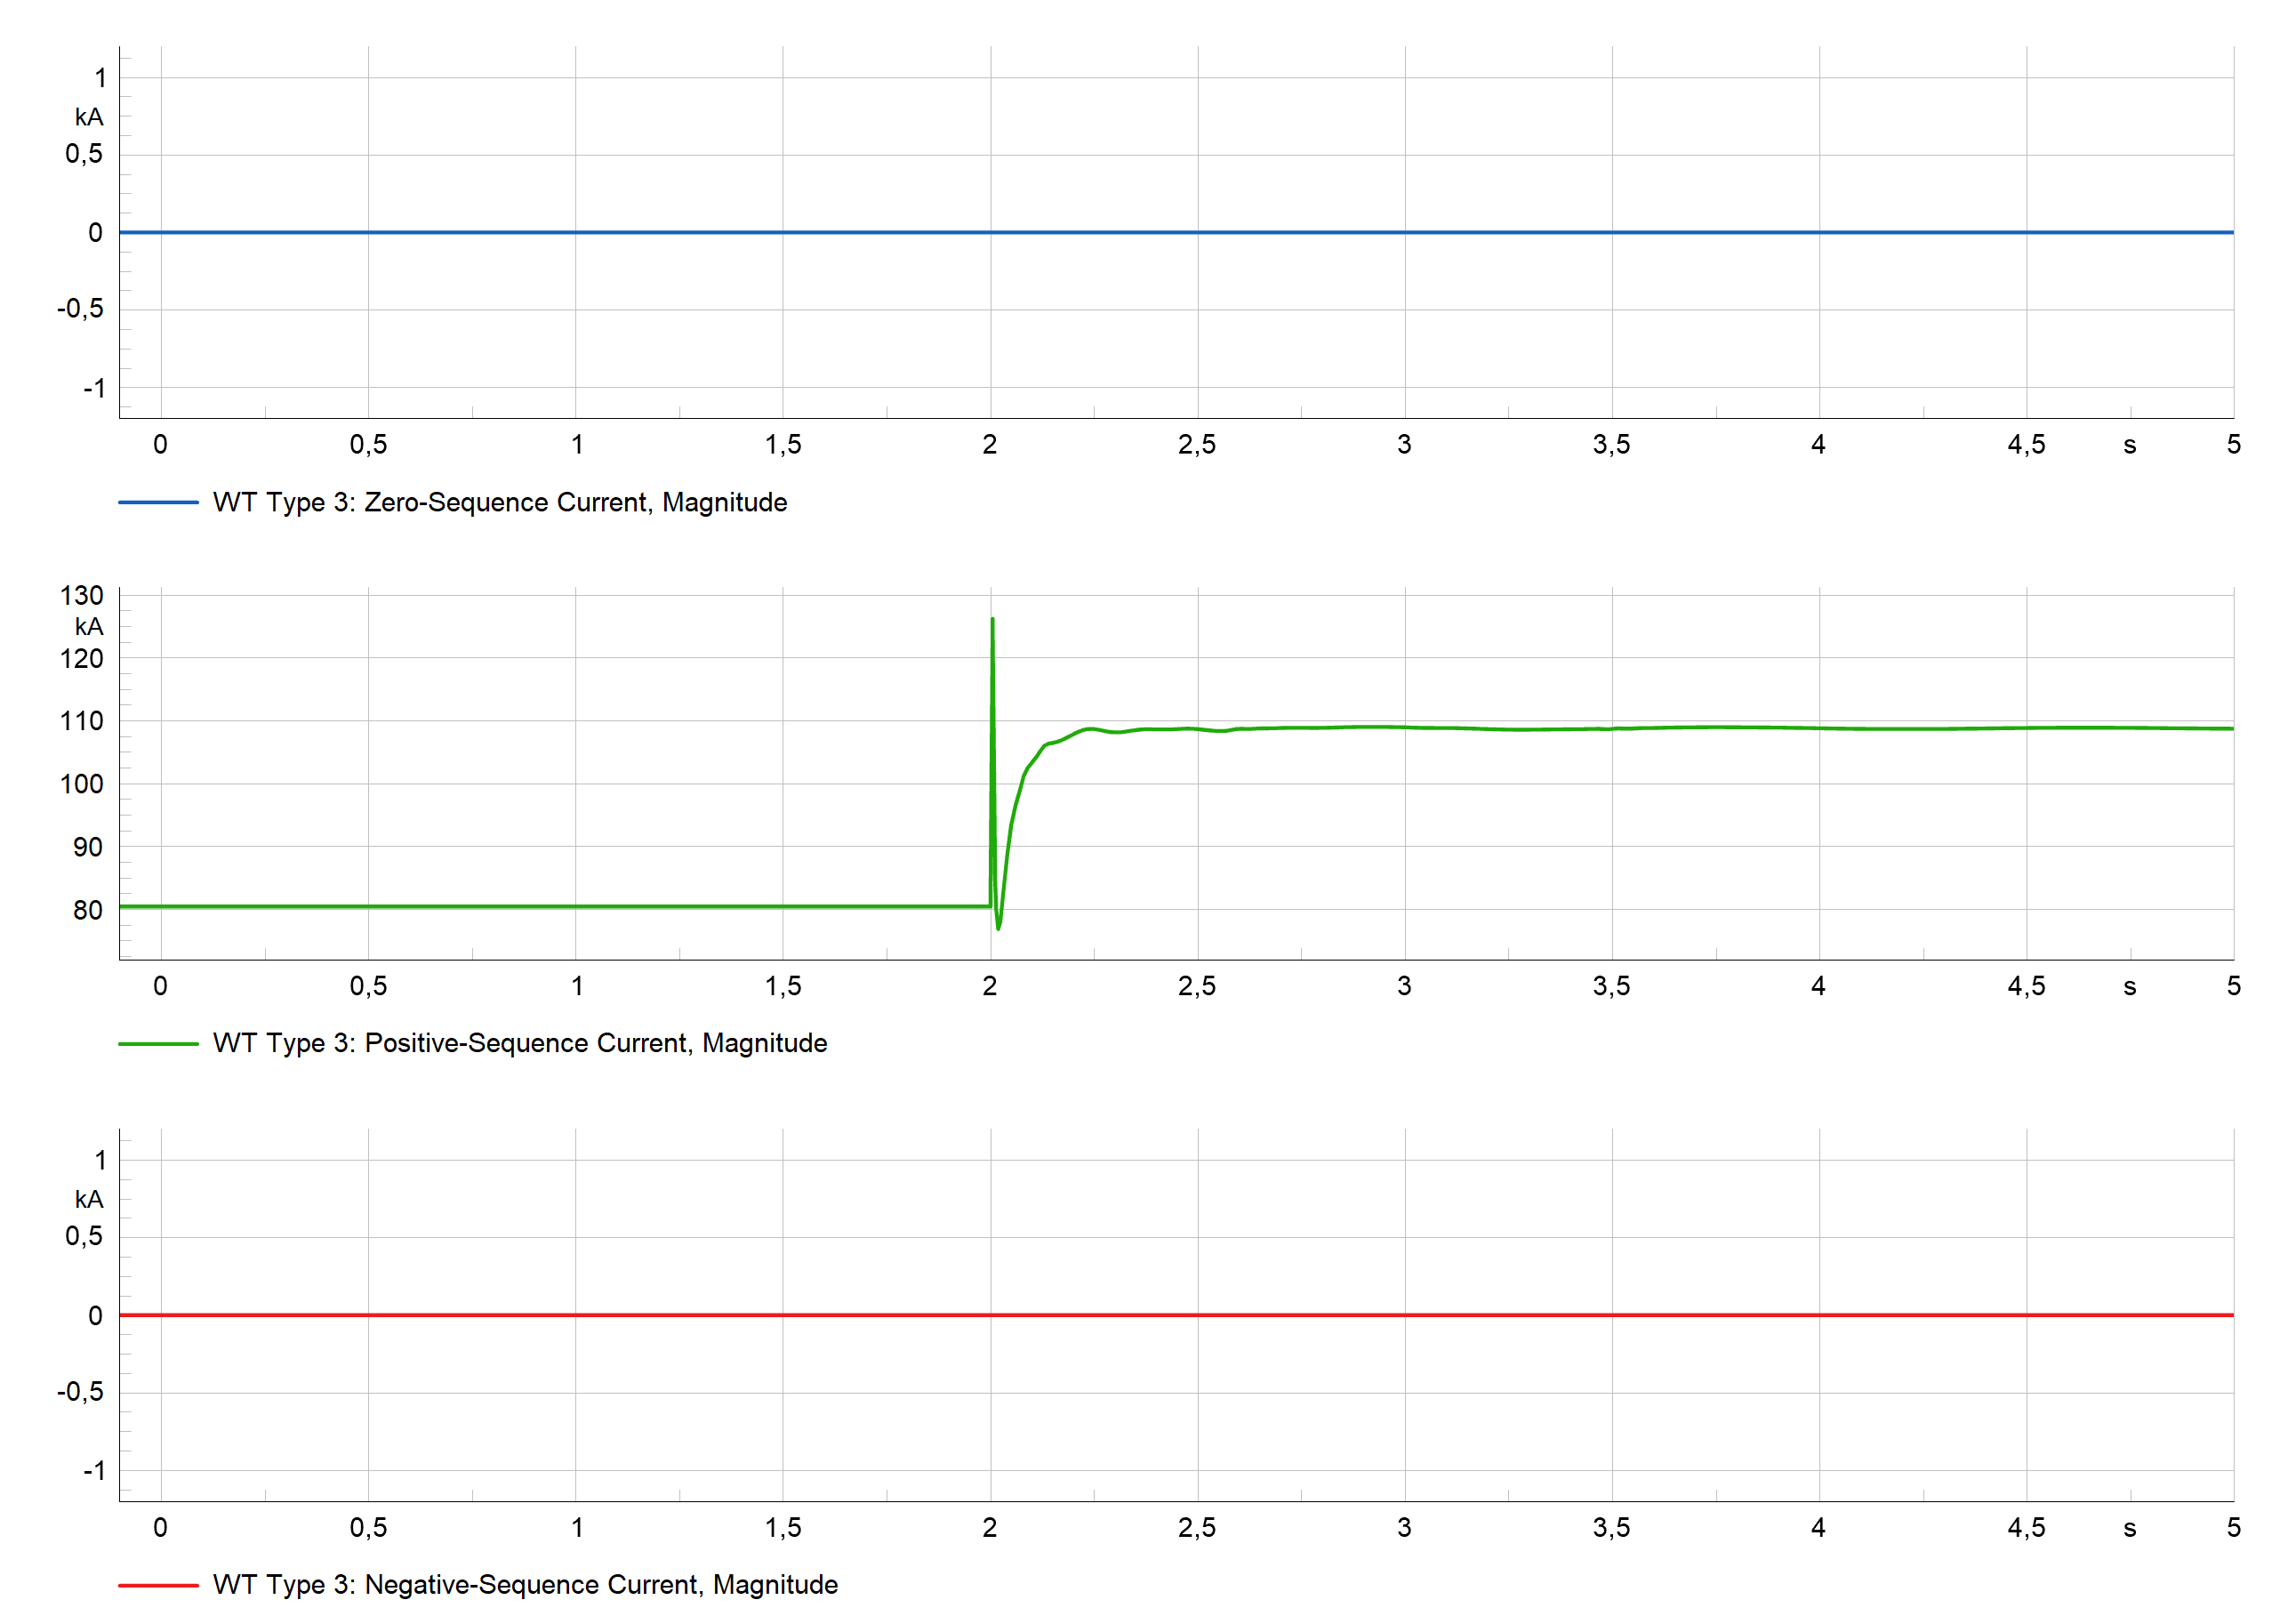
\includegraphics[width=\textwidth]{contents/chapter-4/WTT3_seq_external_3p.png}
        \caption{\textit{Wind Turbine Type 3}.}
        \label{fig:sequence_current_wtt3_s4}
    \end{subfigure}

    \caption{Dekomposisi Komponen Urutan Arus pada Skenario 4}
    \label{fig:decomposition_sequence_current_s4}
\end{figure}

\subsection{Skenario 5: WT Type 3 External SLG Fault}

\begin{figure}[H]
    \centering

    % Gambar sebelah kiri
    \begin{subfigure}[t]{0.48\textwidth}
        \centering
        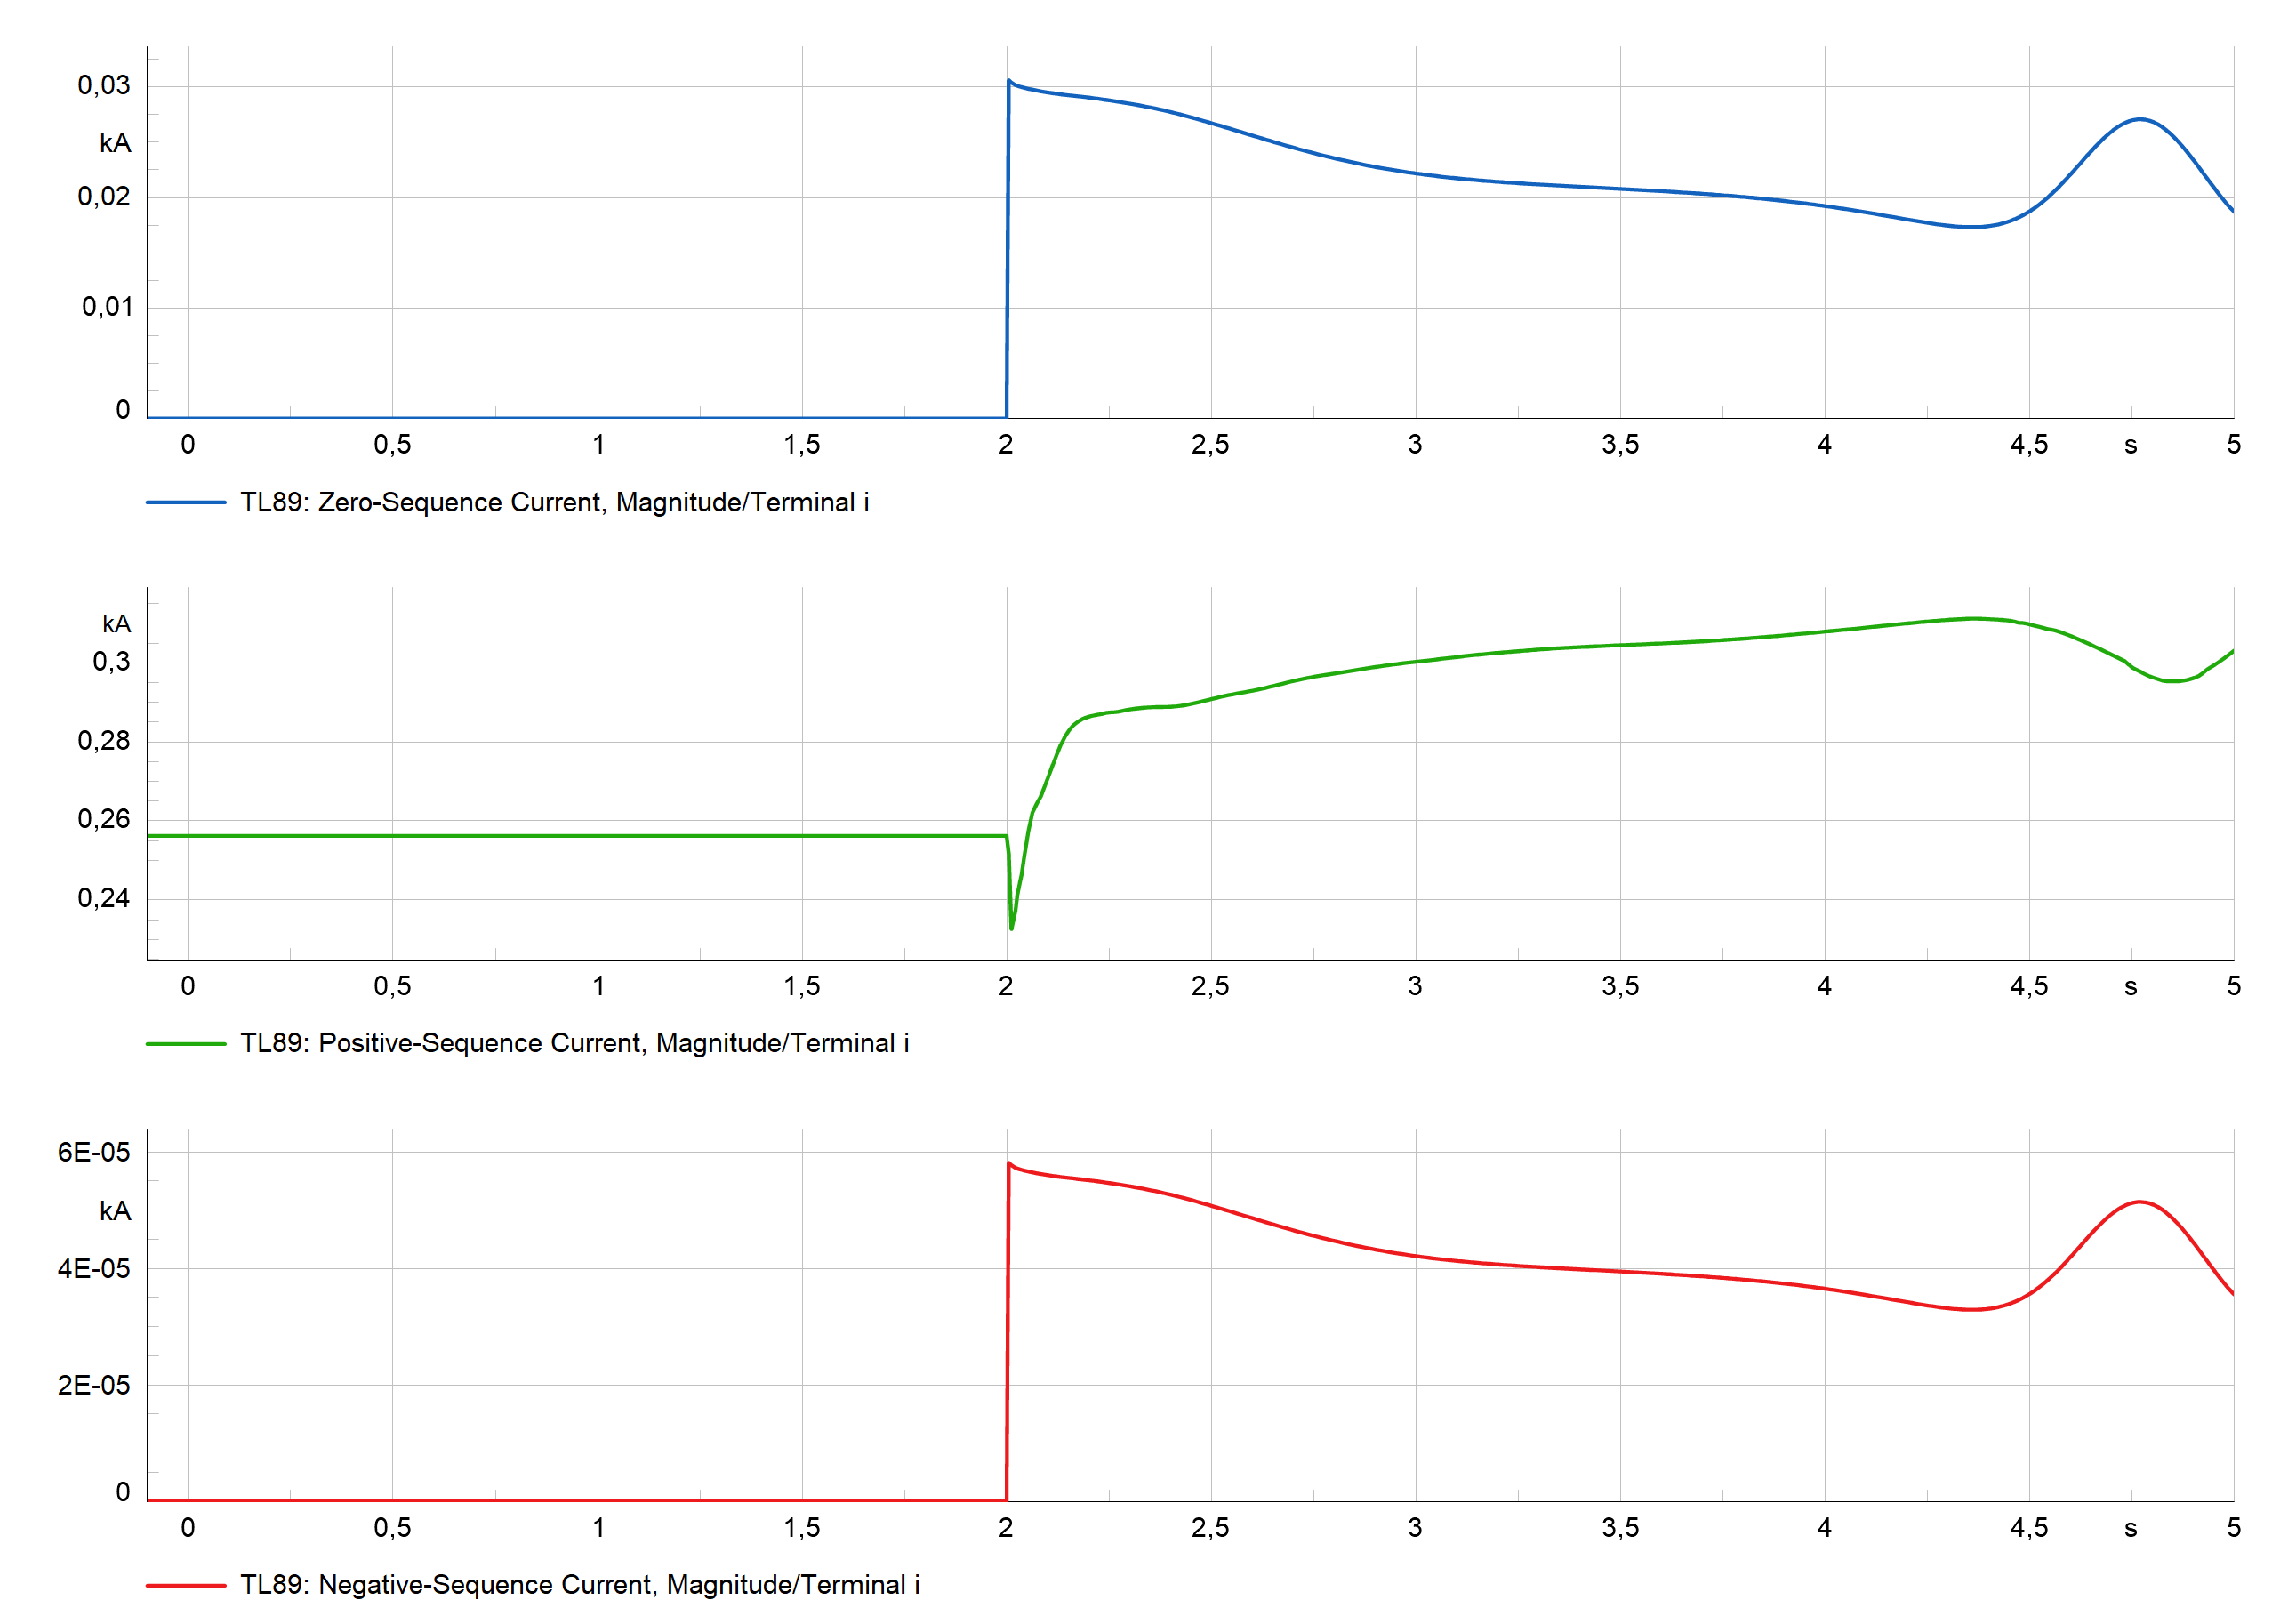
\includegraphics[width=\textwidth]{contents/chapter-4/TL89_seq_s5.png}
        \caption{Saluran TL89}
        \label{fig:sequence_current_tl89_s5}
    \end{subfigure}
    \hfill
    % Gambar sebelah kanan
    \begin{subfigure}[t]{0.48\textwidth}
        \centering
        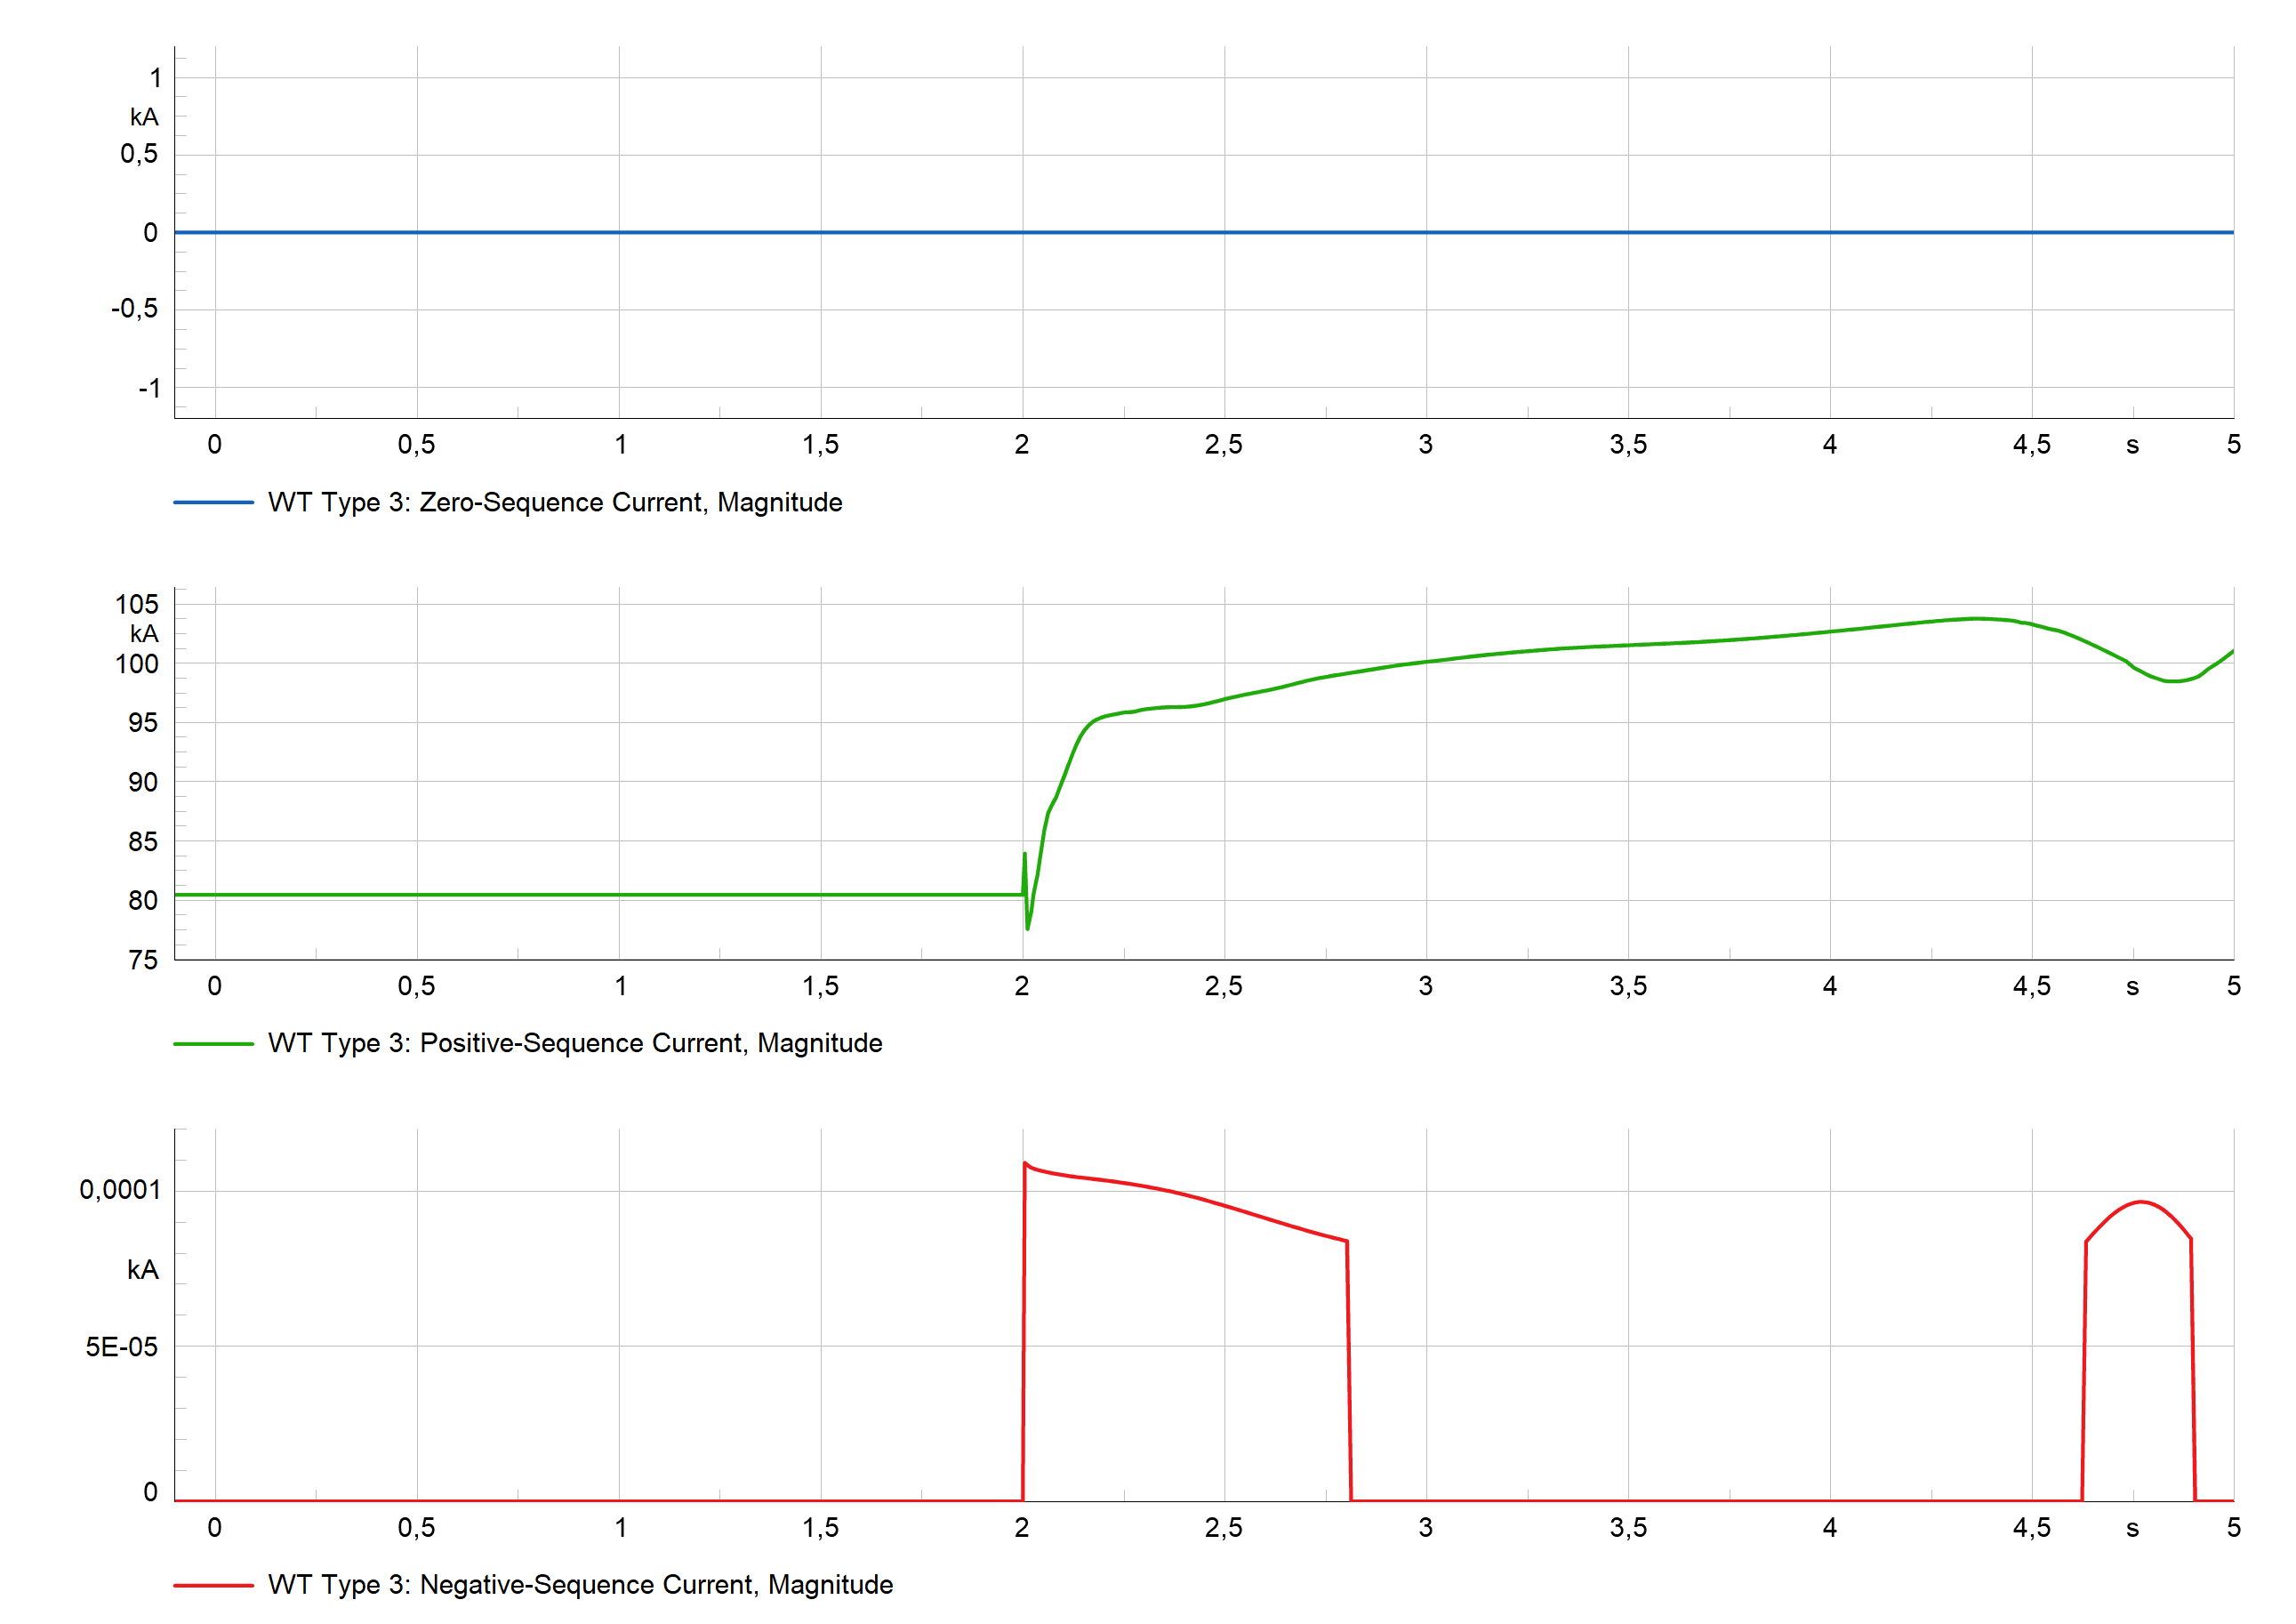
\includegraphics[width=\textwidth]{contents/chapter-4/WTT3_seq_external_slg.png}
        \caption{\textit{Wind Turbine Type 3}.}
        \label{fig:sequence_current_wtt3_s5}
    \end{subfigure}

    \caption{Dekomposisi Komponen Urutan Arus pada Skenario 5}
    \label{fig:decomposition_sequence_current_s5}
\end{figure}

\subsection{Skenario 6: Photovoltaic External DLG Fault}

\begin{figure}[H]
    \centering

    % Gambar sebelah kiri
    \begin{subfigure}[t]{0.48\textwidth}
        \centering
        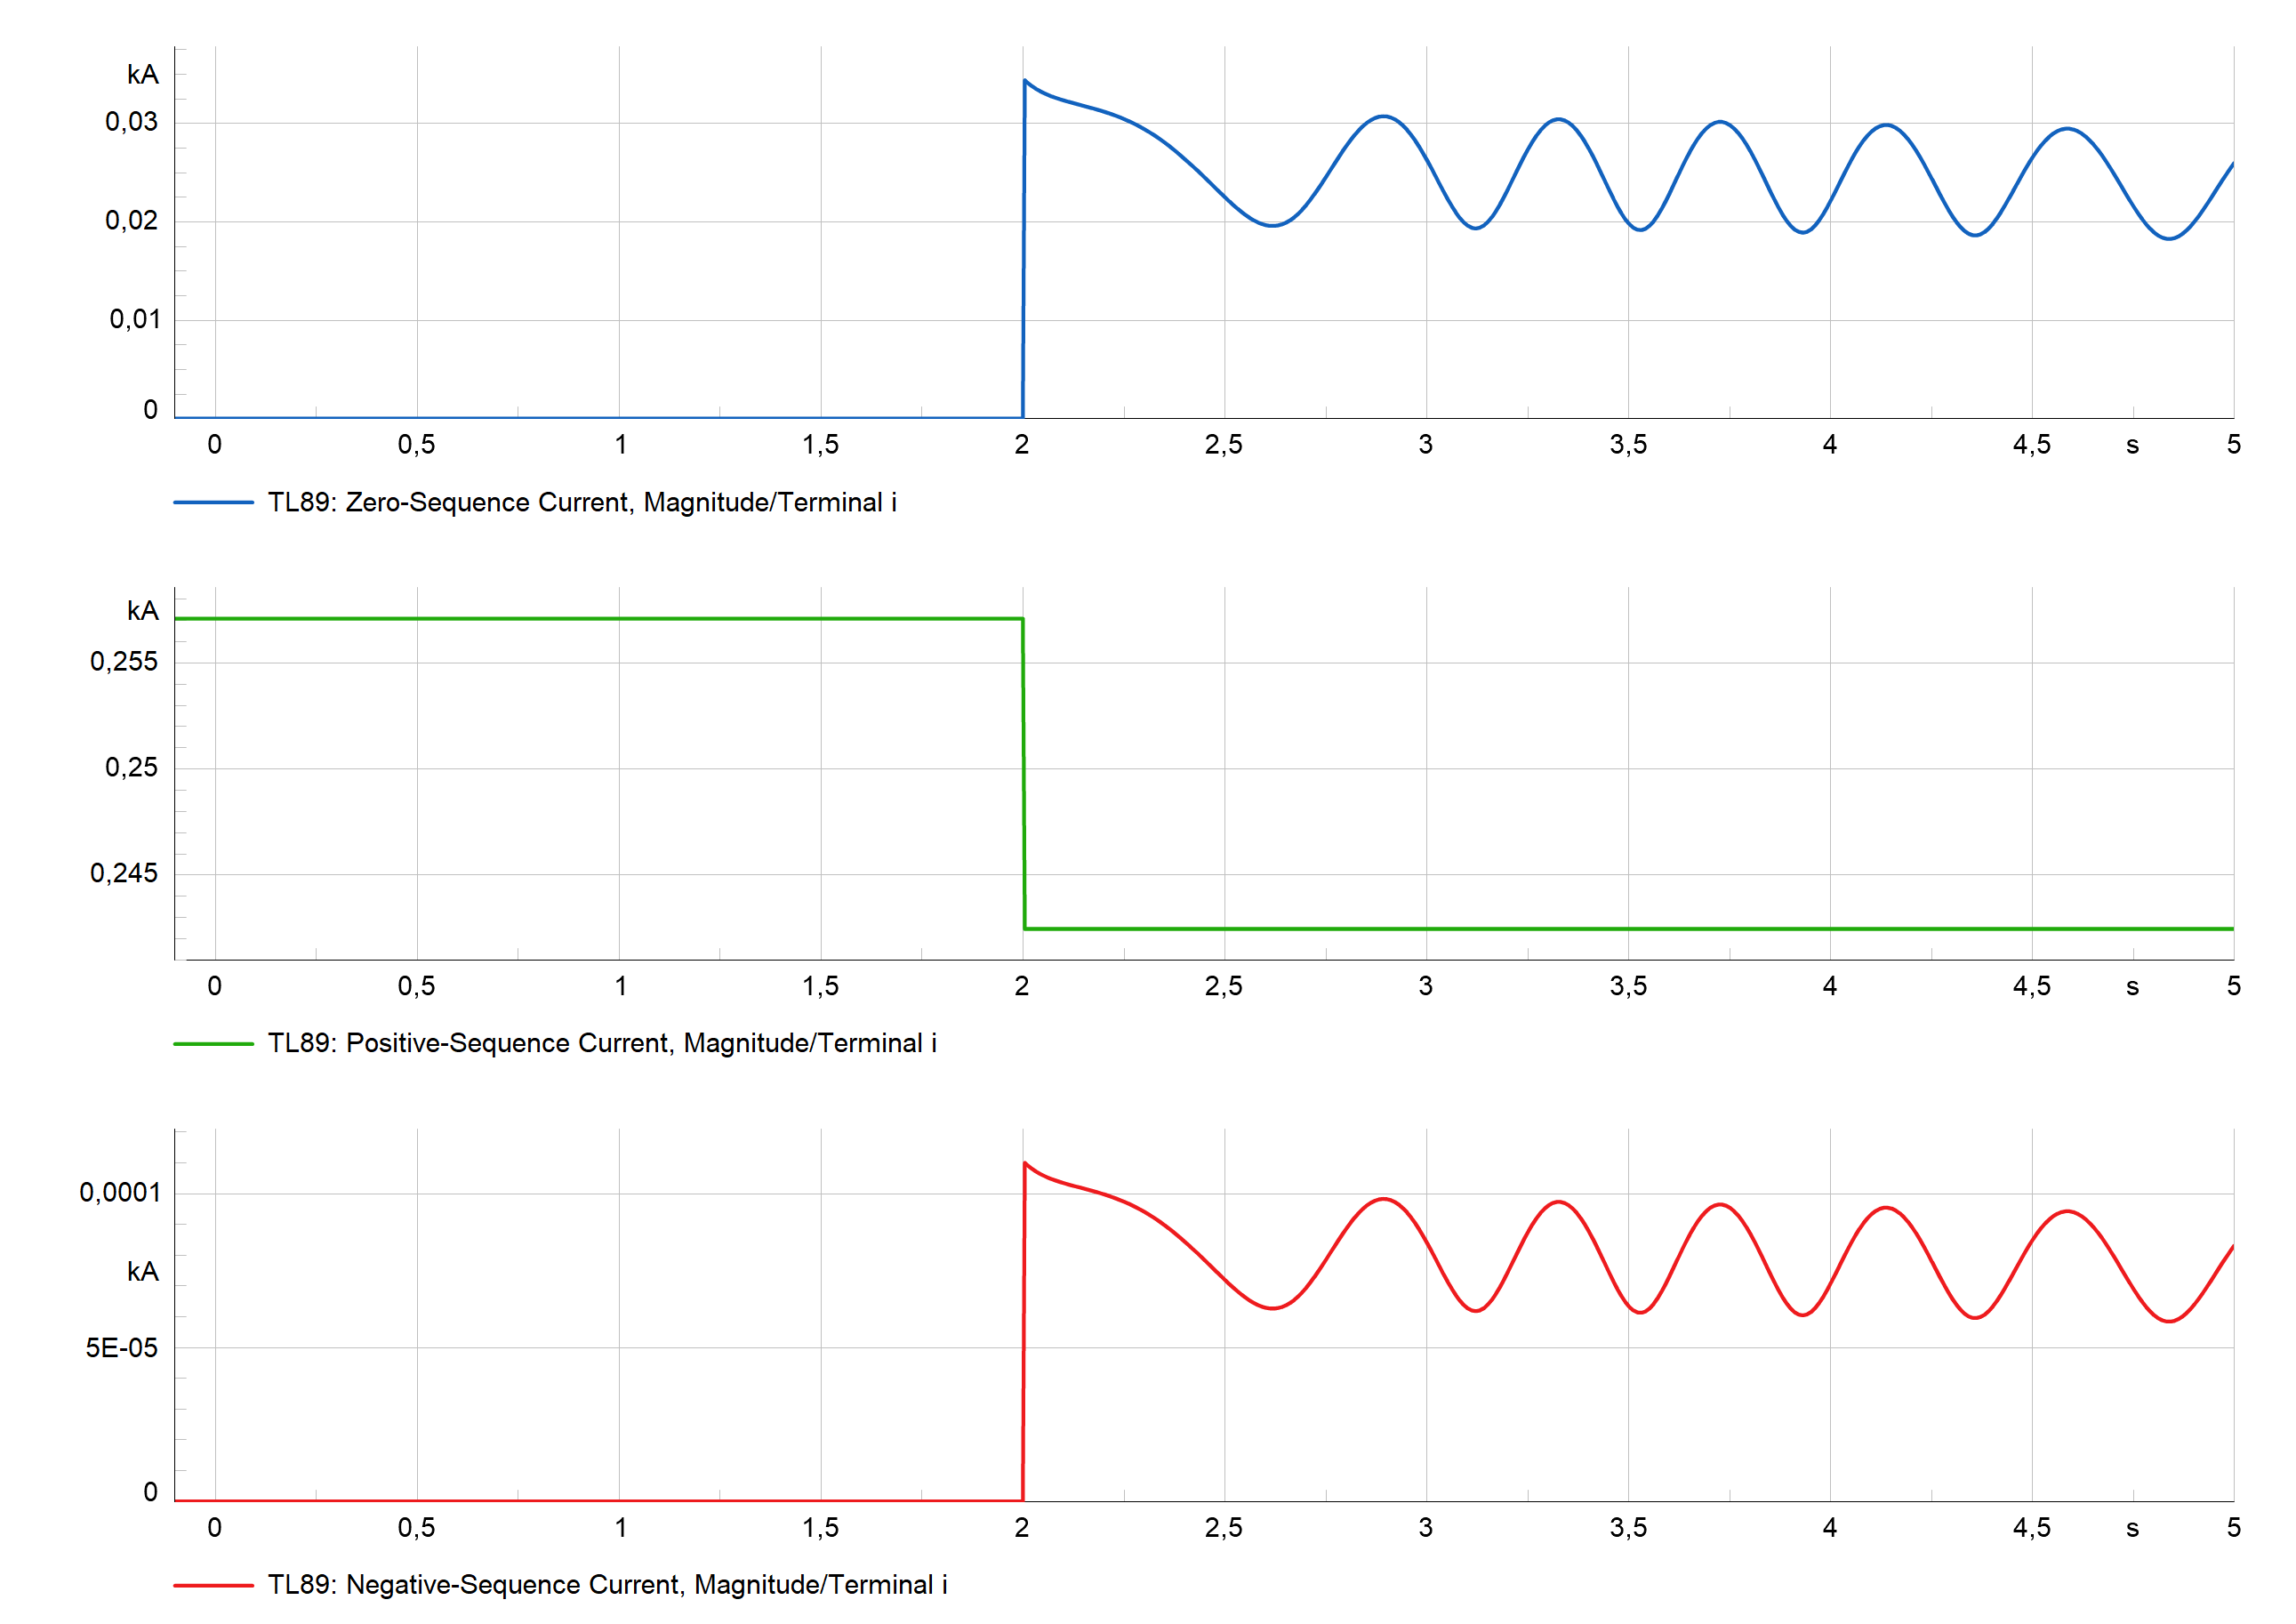
\includegraphics[width=\textwidth]{contents/chapter-4/TL89_seq_s6.png}
        \caption{Saluran TL89}
        \label{fig:sequence_current_tl89_s6}
    \end{subfigure}
    \hfill
    % Gambar sebelah kanan
    \begin{subfigure}[t]{0.48\textwidth}
        \centering
        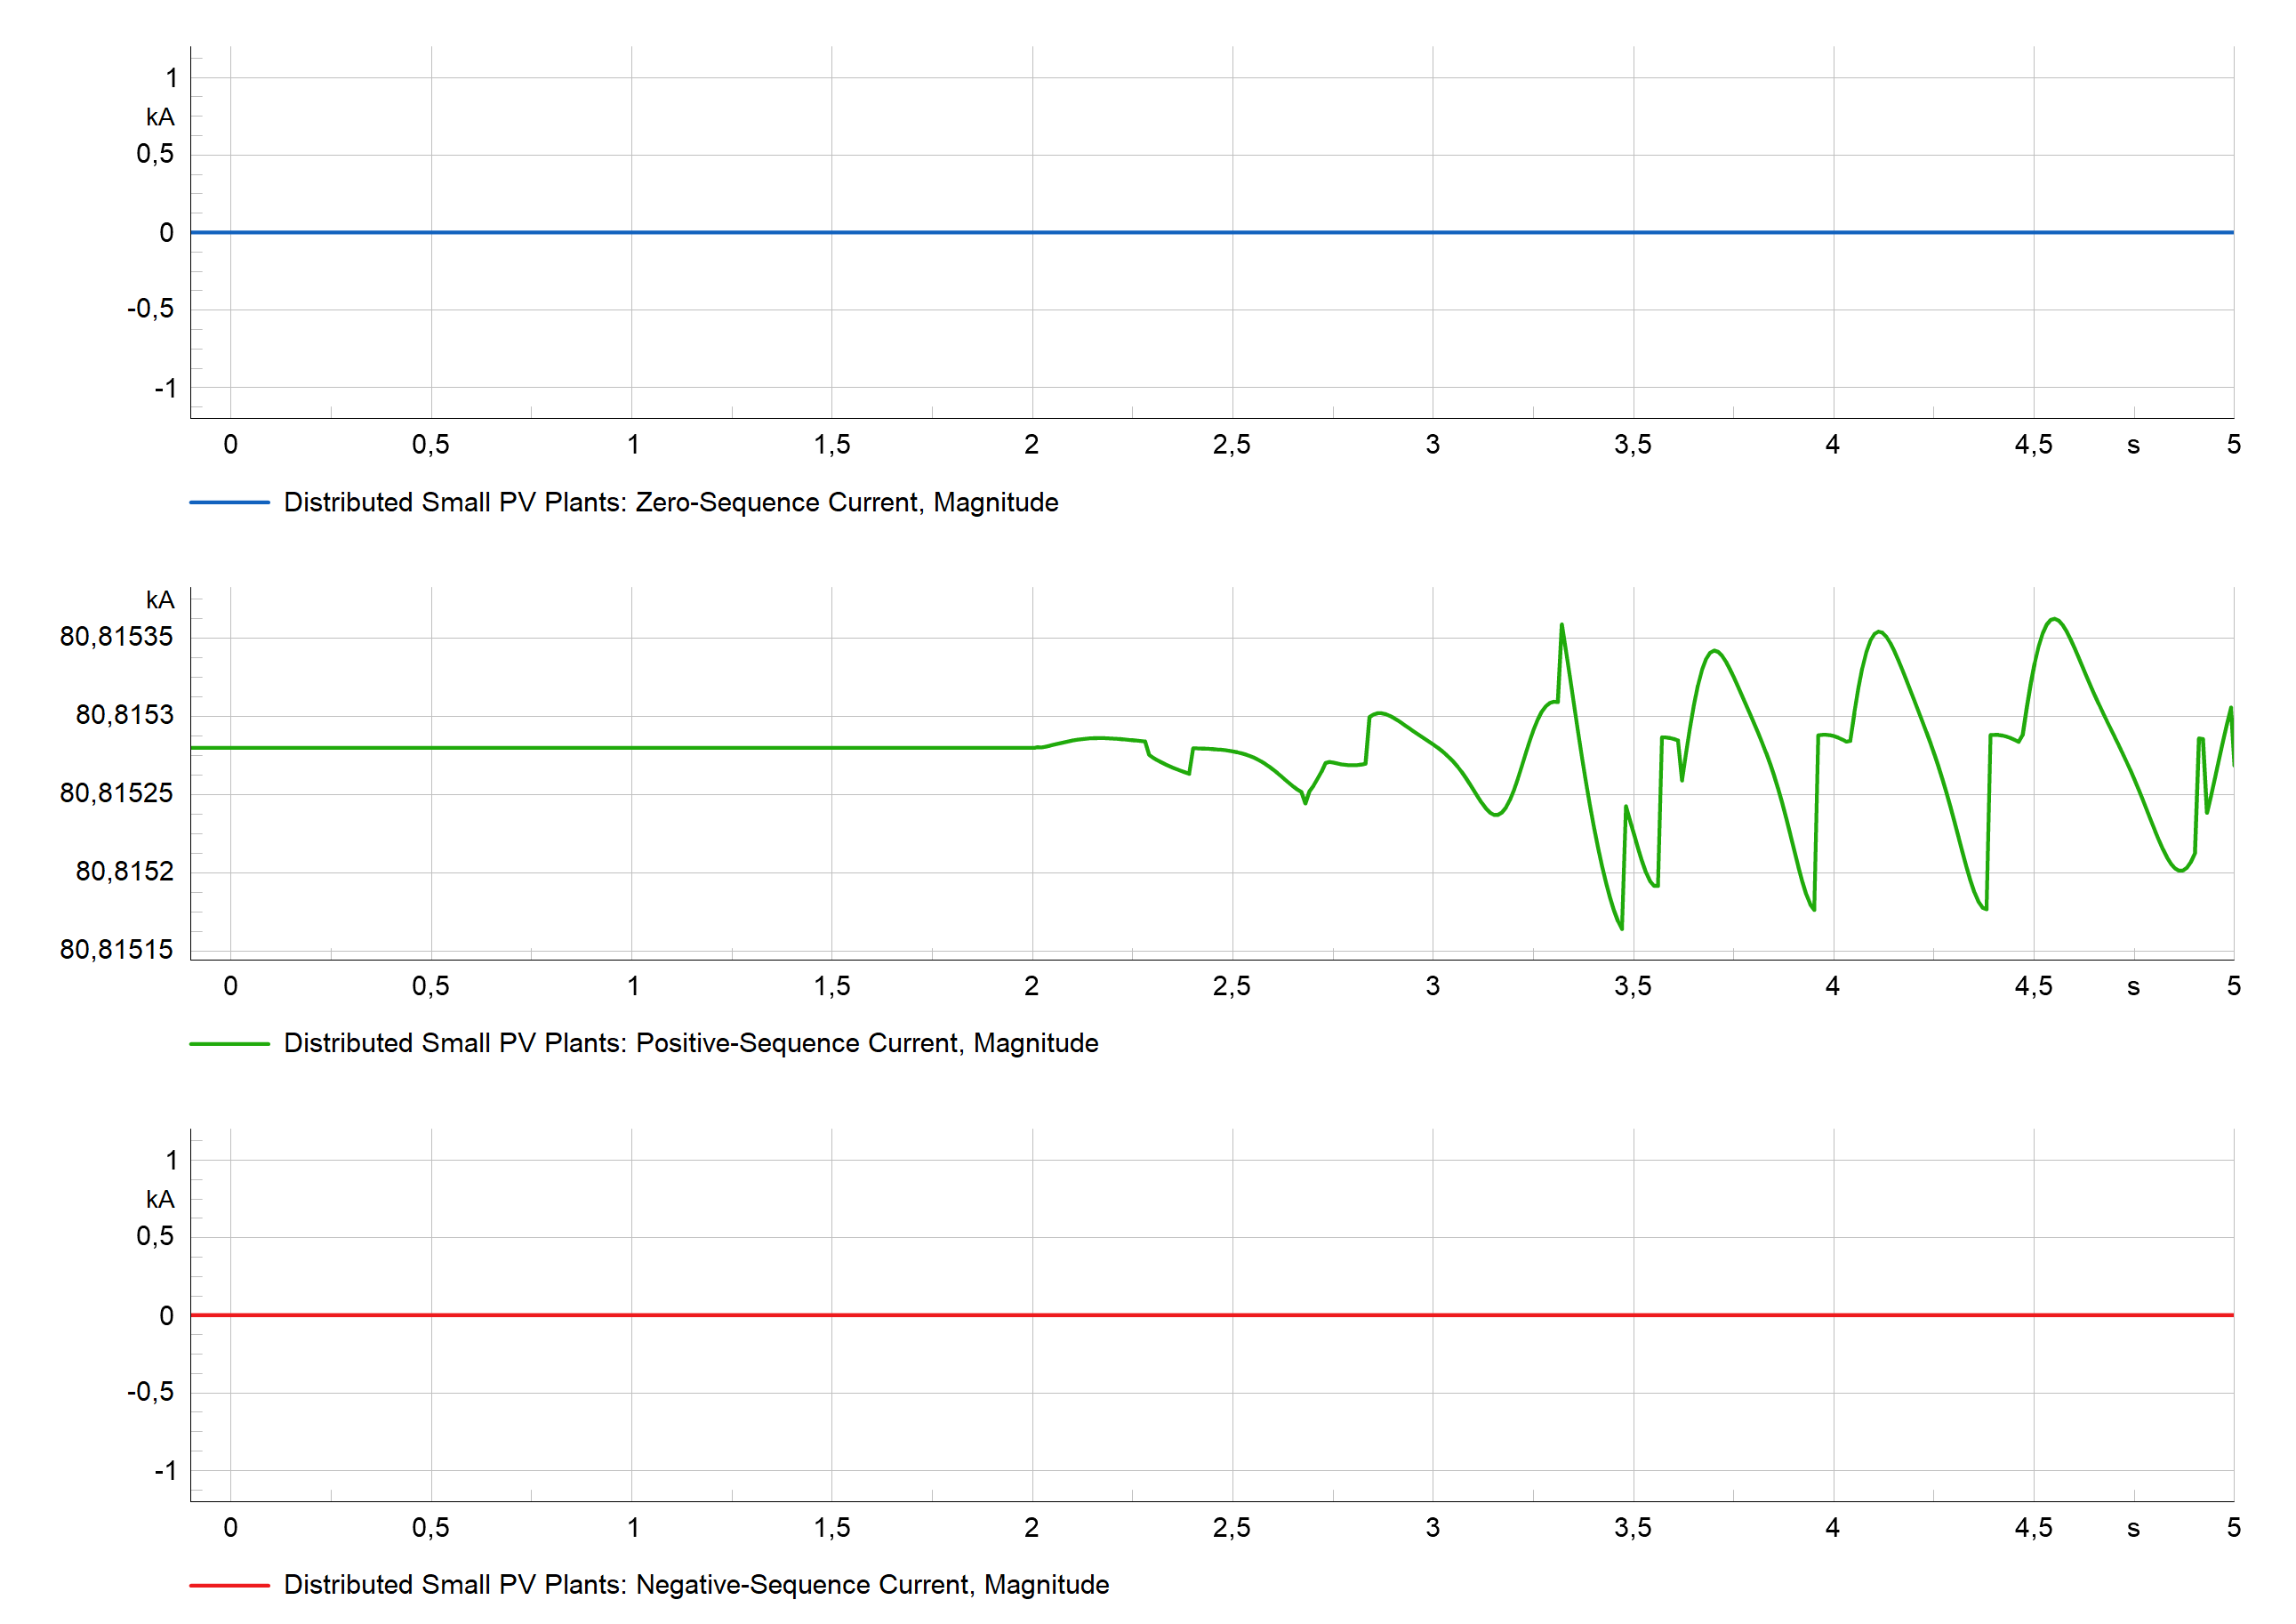
\includegraphics[width=\textwidth]{contents/chapter-4/PV_seq_external_dlg.png}
        \caption{\textit{Photovoltaic}.}
        \label{fig:sequence_current_pv_s6}
    \end{subfigure}

    \caption{Dekomposisi Komponen Urutan Arus pada Skenario 6}
    \label{fig:decomposition_sequence_current_s6}
\end{figure}


\section{Respons Relay 21 pada Sistem dengan WT Type 3}

Bagian ini membahas respons relay 21 ketika sistem diintegrasikan dengan \textit{wind turbine type 3}. Skenario yang diamati mencakup gangguan internal pada TL89 serta gangguan eksternal pada TL79 dengan kondisi saluran tertentu \textit{out of service}, sesuai skenario pengujian pada Bab III. Analisis dilakukan dengan membandingkan impedansi tampak, arah gangguan, dan keputusan trip terhadap kondisi dasar tanpa IBR.

Pada setiap skenario, pembacaan relay dari sisi Bus 8 dan Bus 9 dibahas secara terpisah. Pemisahan ini diperlukan karena kedua sisi relay dapat menerima kontribusi arus gangguan yang berbeda, sehingga keputusan operasi relay 21 dapat berbeda antara ujung saluran yang satu dan ujung saluran yang lain.

\subsection{Skenario 1 : Wind Turbine Type 3 Internal DLG Fault}

Skenario ini menjadi titik awal pembahasan respons relay 21 pada sistem dengan \textit{wind turbine type 3} karena gangguan ditempatkan pada TL89, yaitu saluran yang diproteksi. Dengan demikian, respons relay yang diharapkan adalah relay dari kedua sisi saluran mampu membaca gangguan sebagai gangguan internal dan memberikan perintah trip sesuai daerah operasi yang terbaca.

Dekomposisi komponen urutan arus pada Gambar \ref{fig:decomposition_sequence_current_s1} digunakan sebagai konteks untuk membaca besaran arus gangguan yang masuk ke relay. Setelah kontribusi arus pada skenario ini diketahui, analisis dilanjutkan pada impedansi tampak yang terbaca pada masing-masing elemen gangguan, yaitu ZAG, ZBG, dan ZAB, dari sisi Bus 8 maupun Bus 9.

% \begin{figure}[H]
%     \centering
%     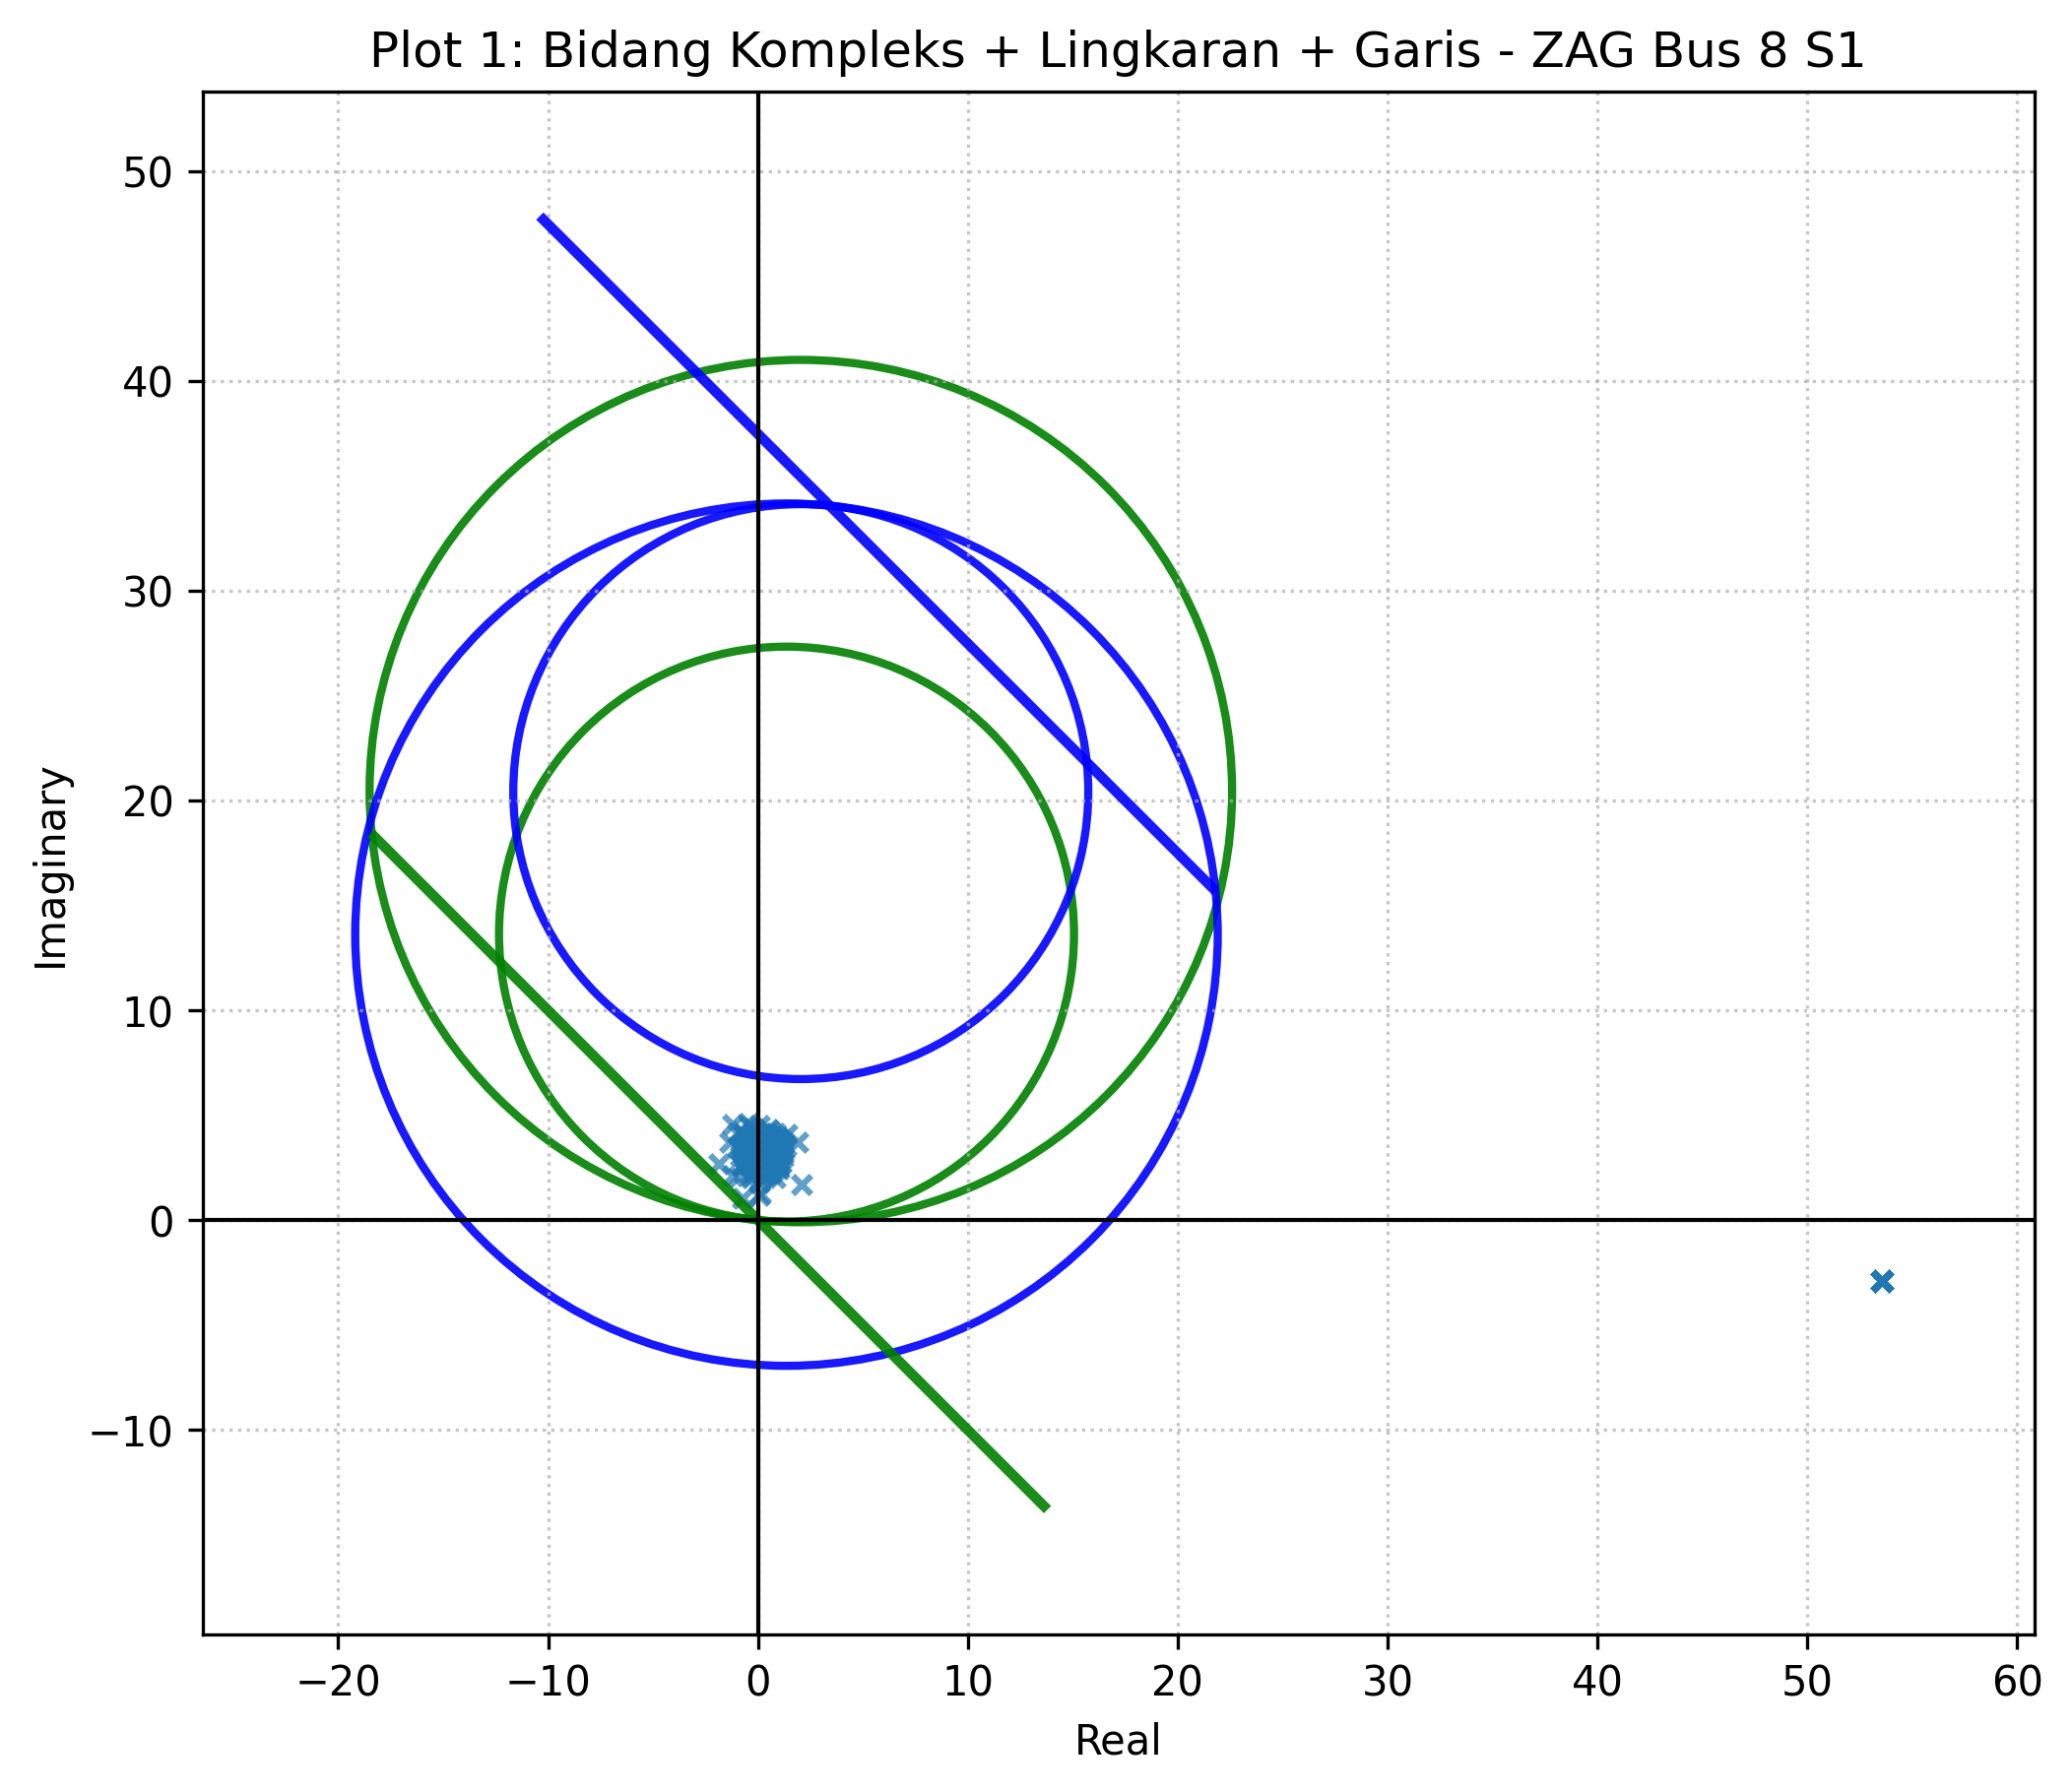
\includegraphics[width=0.8\textwidth]{contents/chapter-4/01_ZAG_Bus_8_S1_dengan_lingkaran_dan_garis.png}
%     \caption{Impedansi Tampak ZAG Bus 8 Skenario 1}
%     \label{fig:01_ZAG_Bus_8_S1_dengan_lingkaran_dan_garis}
% \end{figure}

% Pada gambar \ref{fig:01_ZAG_Bus_8_S1_dengan_lingkaran_dan_garis} terlihat untuk titik impedansi tampak pada fasa A dan ground terlihat cukup stabil dan relay 21 dari sisi bus 8 bekerja dengan normal sebagaimana mestinya dengan acuan pada \ref{subsec:tanpa_IBR_in_dlg} karena kontribusi dari sisi IBR tidak mendominasi karena TL78 tetap aktif mengakibatkan IBR tidak memengaruhi kinerja proteksi serta kontribusi tetap di dominasi oleh sistem tenaga konvensional.

%%%%%%%%%%%%%%%%%%%%%%%%%%%%%%%%%SISI PRIMER%%%%%%%%%%%%%%%%%%%%%%%%%%%%%%%%%%

% \begin{figure}[H]
%     \centering
%     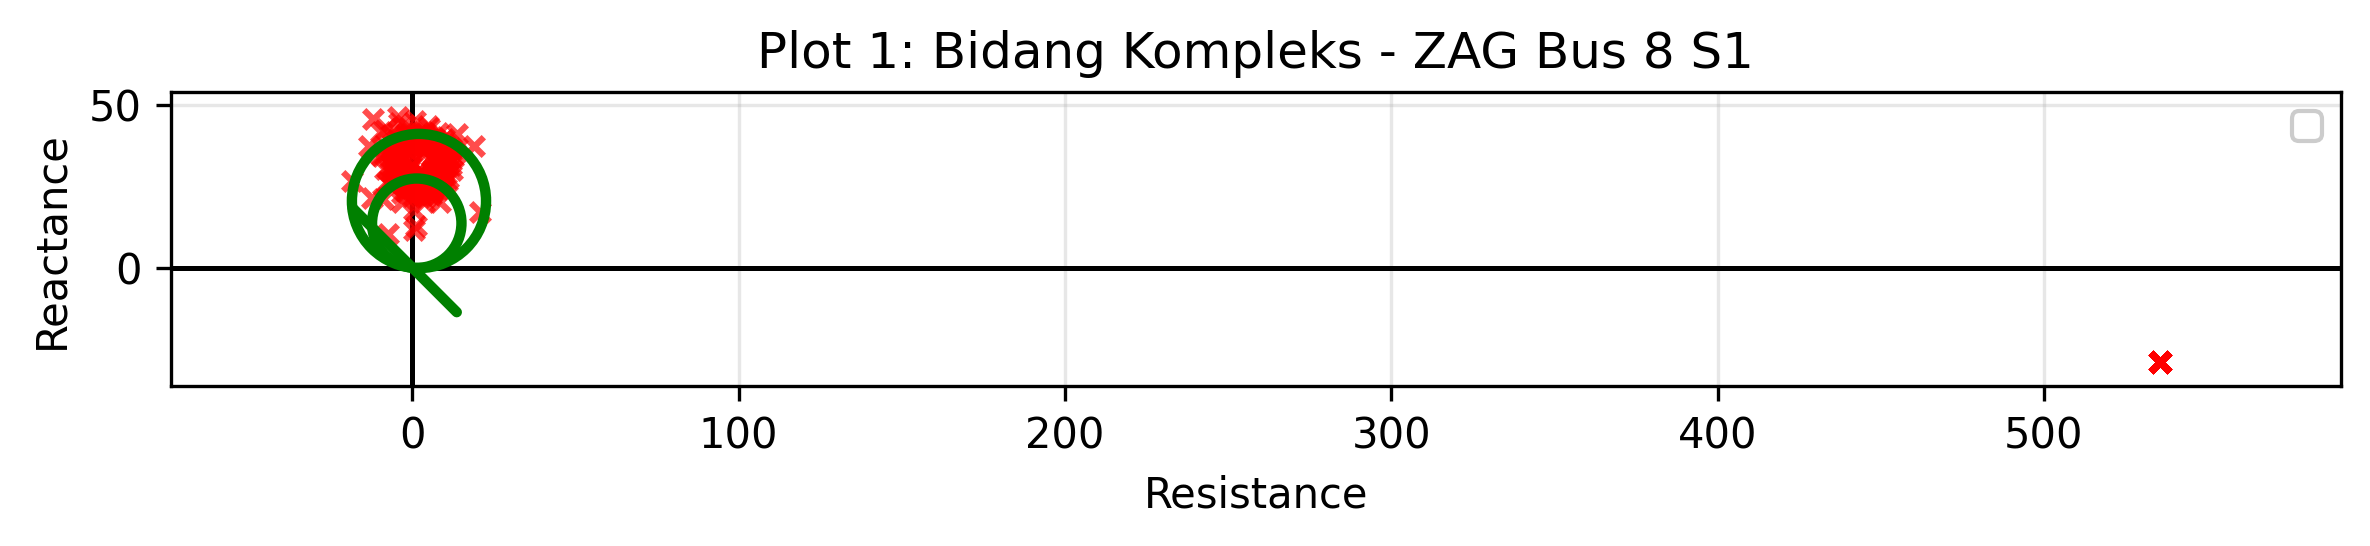
\includegraphics[width=0.8\textwidth]{contents/chapter-4/PRIA_01_ZAG_Bus_8_S1.png}
%     \caption{Impedansi Tampak ZAG Bus 8 Skenario 1}
%     \label{fig:PRIA_01_ZAG_Bus_8_S1}
% \end{figure}

% \begin{figure}[H]
%     \centering
%     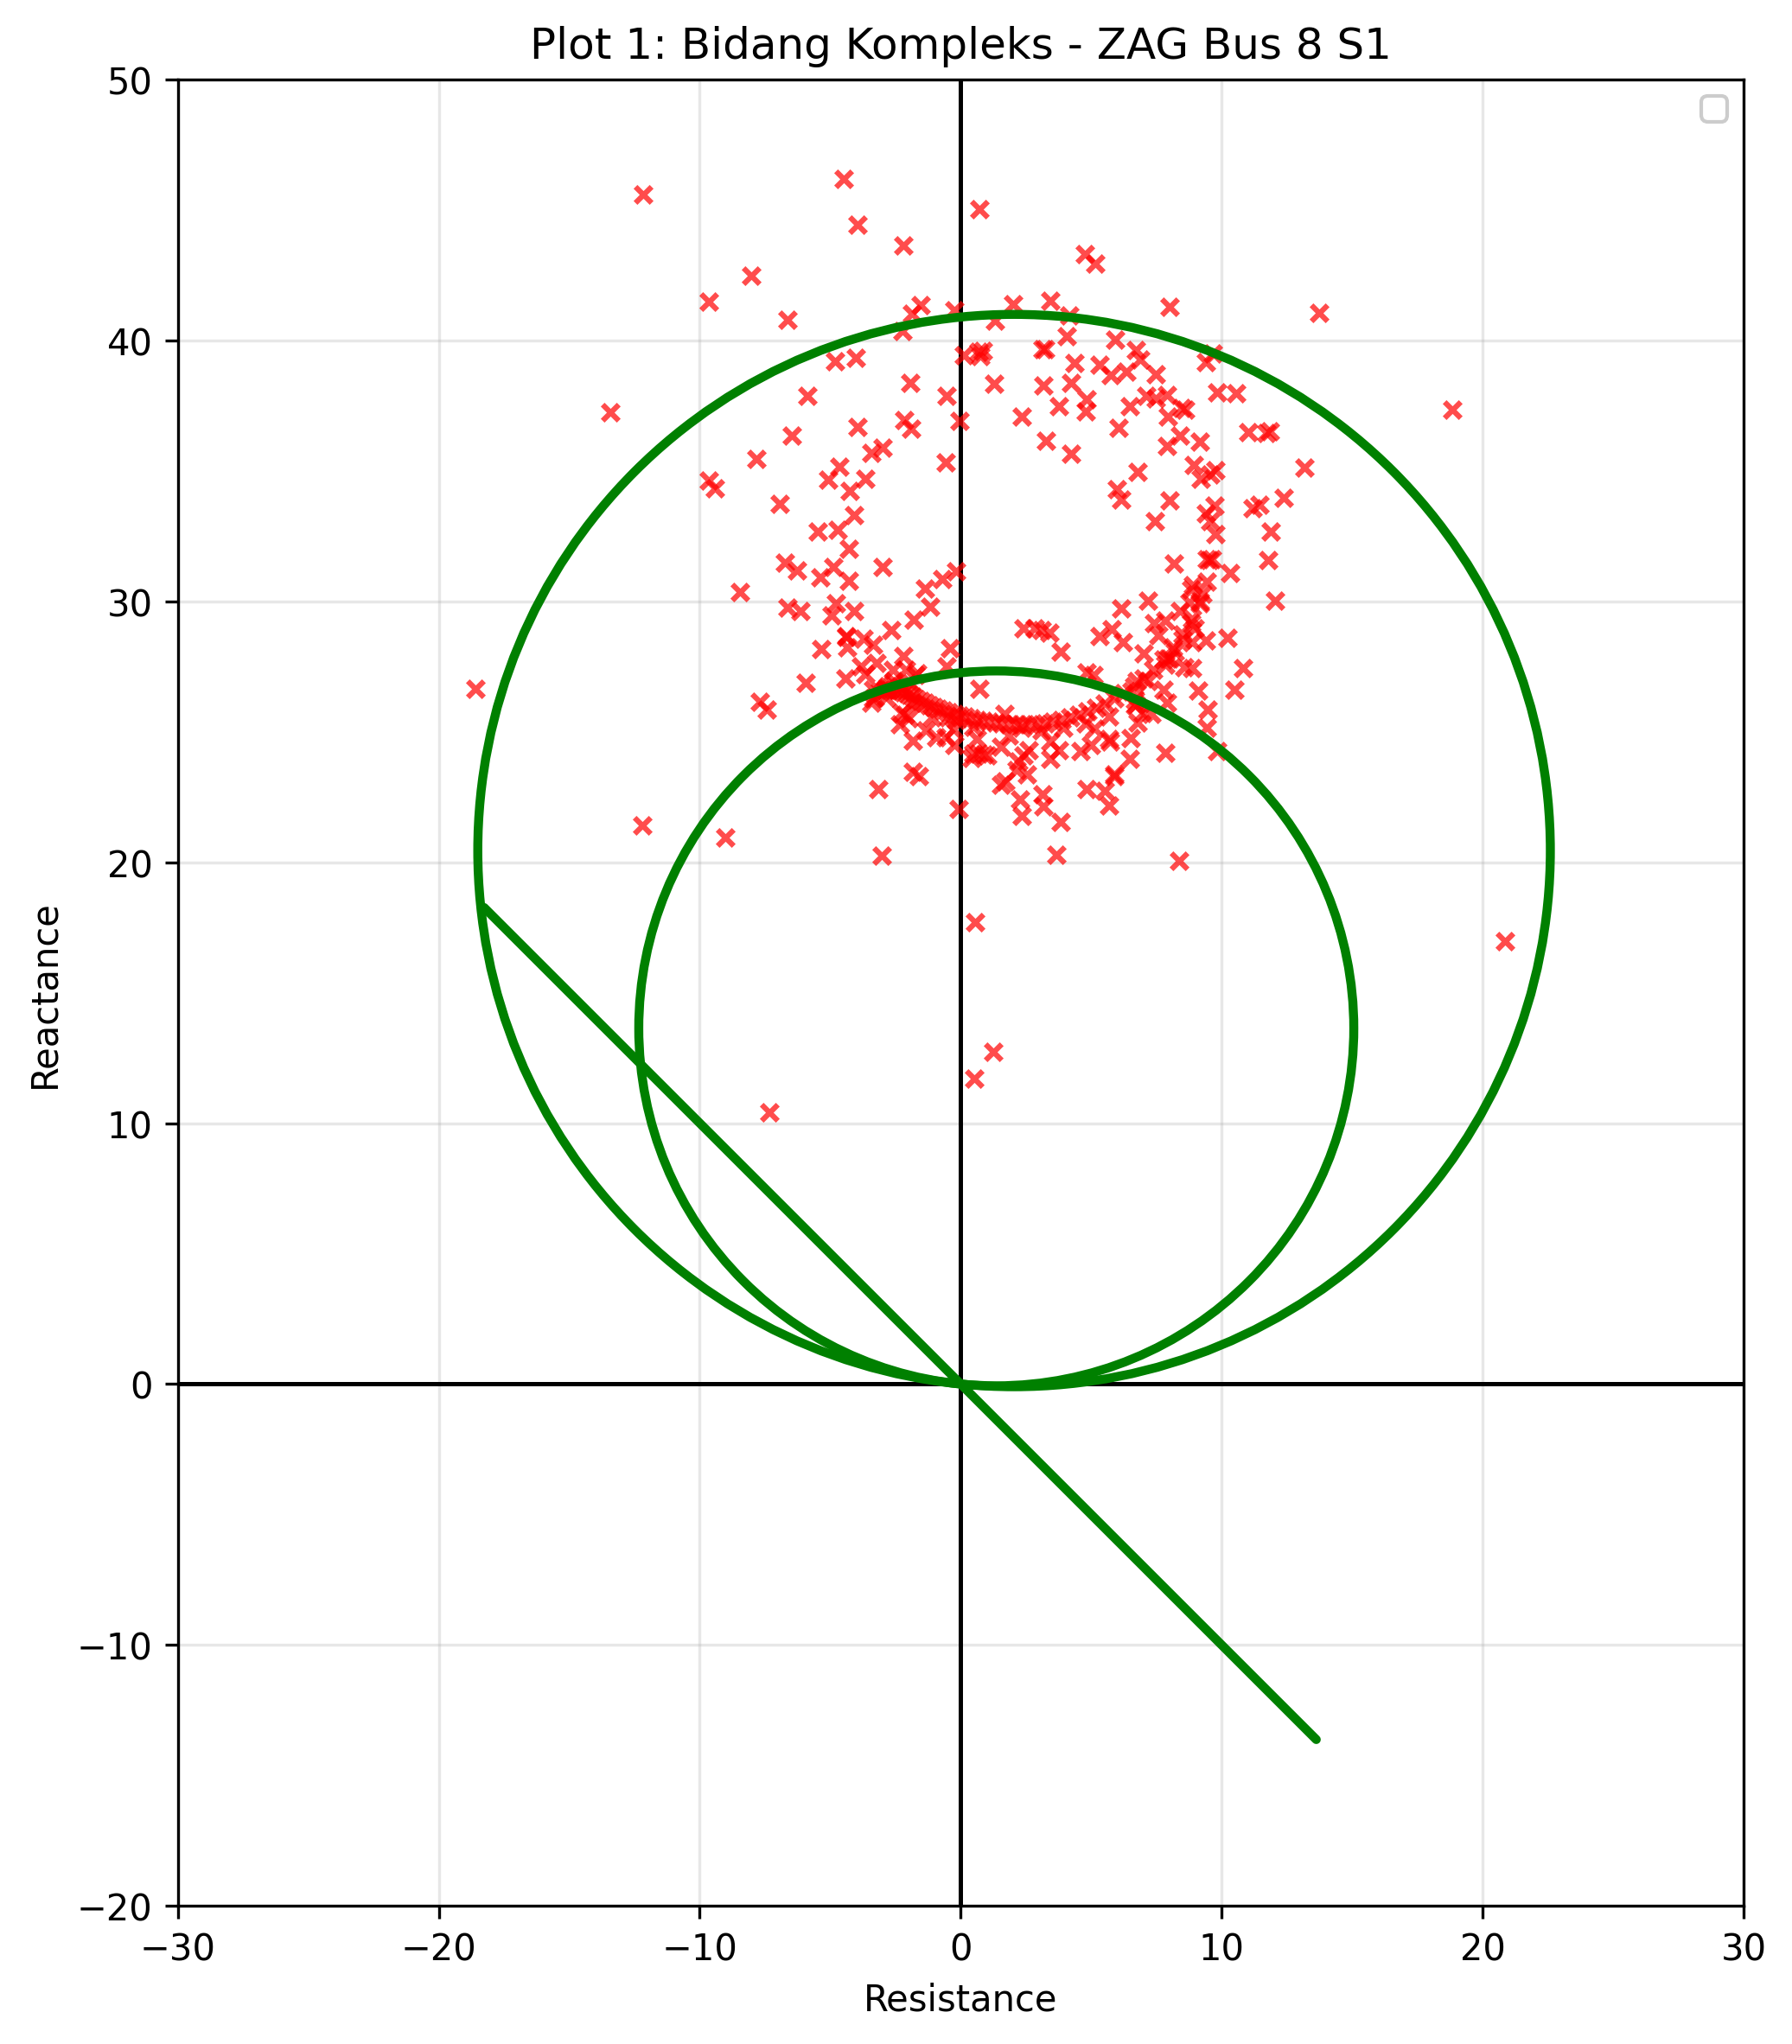
\includegraphics[width=0.8\textwidth]{contents/chapter-4/PRIZI_01_ZAG_Bus_8_S1.png}
%     \caption{Impedansi Tampak ZAG Bus 8 Skenario 1}
%     \label{fig:PRIZI_01_ZAG_Bus_8_S1}
% \end{figure}

\begin{figure}[H]
    \centering

    % Gambar sebelah kiri
    \begin{subfigure}[t]{0.48\textwidth}
        \centering
        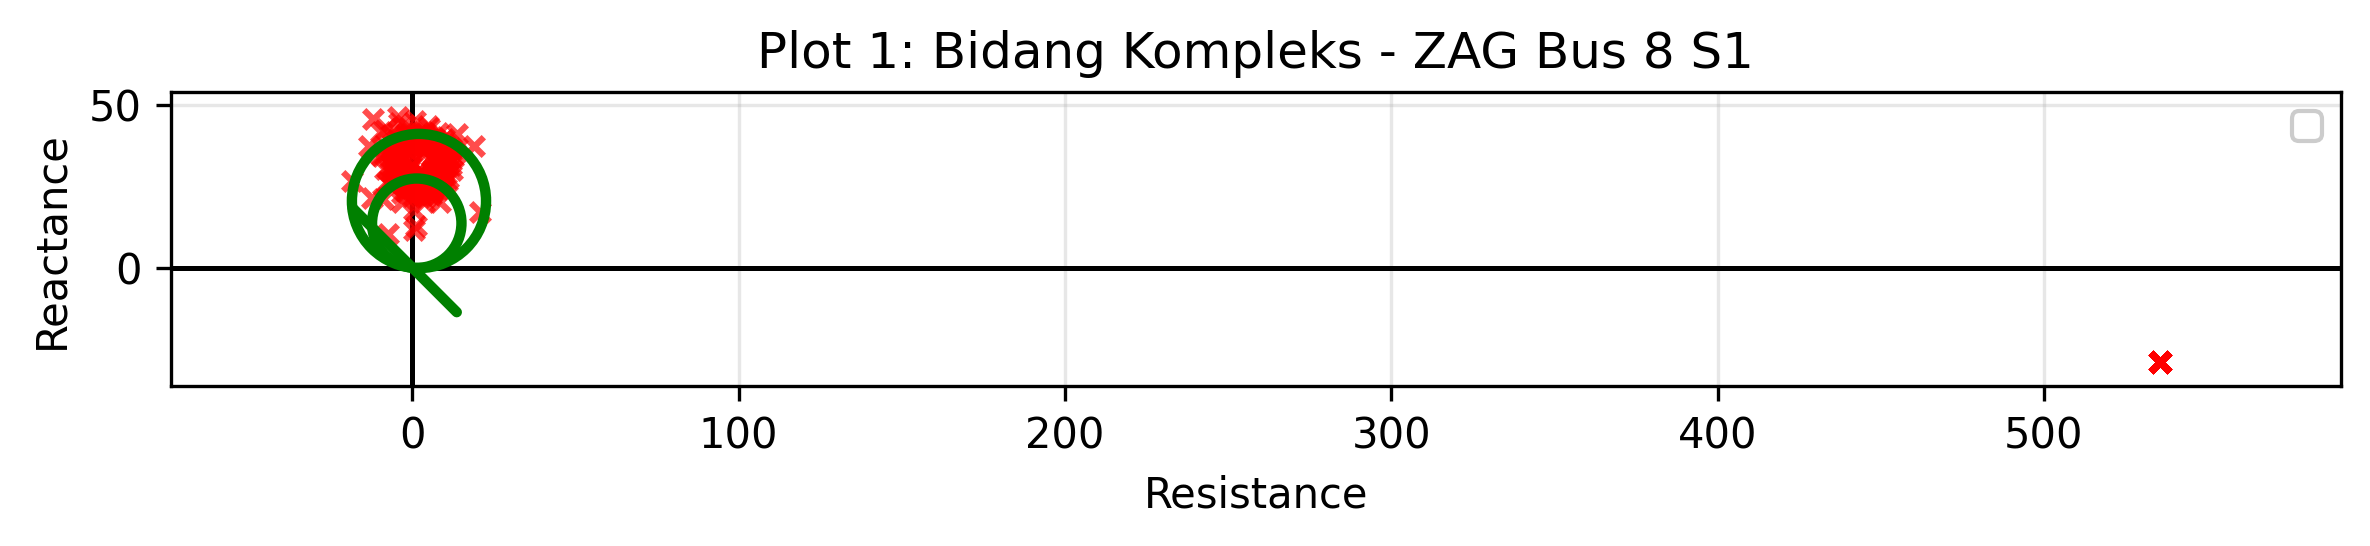
\includegraphics[width=\textwidth]{contents/chapter-4/PRIA_01_ZAG_Bus_8_S1.png}
        \caption{Seluruh Impedansi Tampak}
        \label{fig:PRIA_01_ZAG_Bus_8_S1}
    \end{subfigure}
    \hfill
    % Gambar sebelah kanan
    \begin{subfigure}[t]{0.48\textwidth}
        \centering
        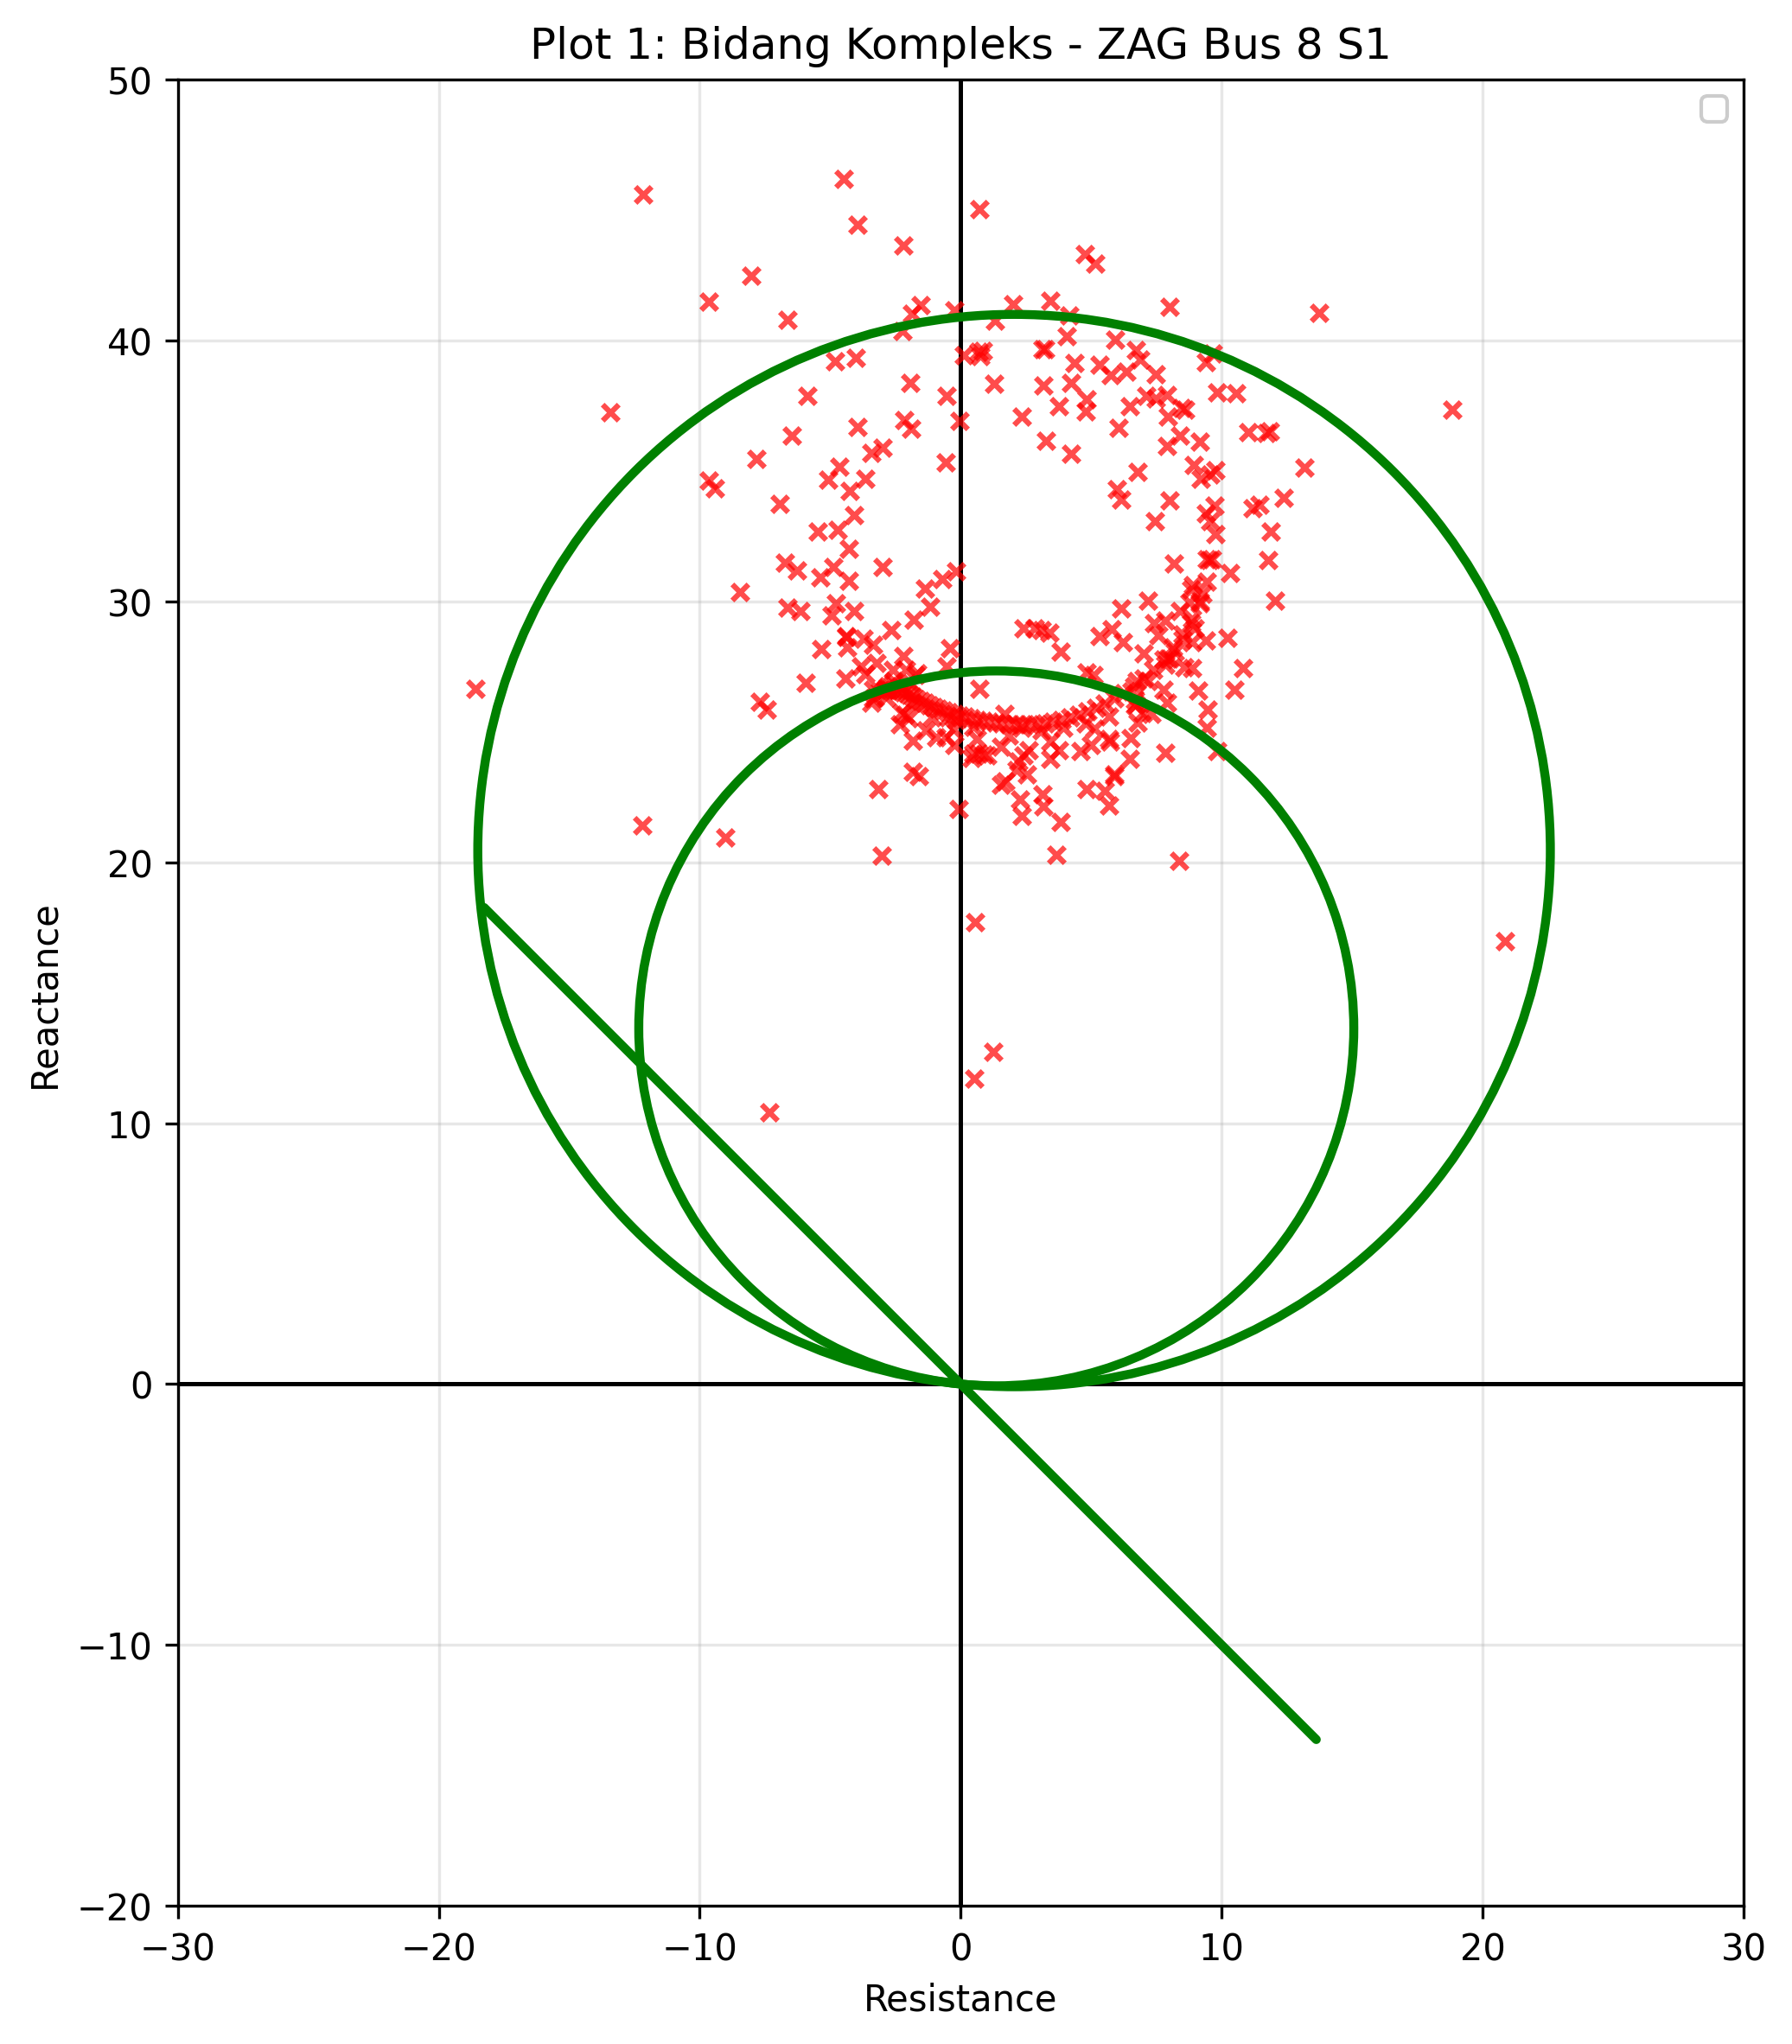
\includegraphics[width=\textwidth]{contents/chapter-4/PRIZI_01_ZAG_Bus_8_S1.png}
        \caption{Zoom In Pada Zona Proteksi}
        \label{fig:PRIZI_01_ZAG_Bus_8_S1}
    \end{subfigure}

    \caption{Impedansi Tampak ZAG Bus 8 Skenario 1}
    \label{fig:Impedansi_Tampak_ZAG_Bus_8_S1}
\end{figure}

Pada gambar \ref{fig:Impedansi_Tampak_ZAG_Bus_8_S1} terlihat untuk titik impedansi tampak pada fasa A dan ground yang dibaca oleh relay 21 dari sisi bus 8 bekerja dengan baik sebagaimana mestinya dengan acuan pada \ref{subsec:tanpa_IBR_in_dlg} karena kontribusi dari sisi IBR tidak mendominasi karena TL78 tetap aktif mengakibatkan IBR tidak memengaruhi kinerja proteksi serta kontribusi tetap di dominasi oleh sistem tenaga konvensional.

%%%%%%%%%%%%%%%%%%%%%%%%%%%%%%%%%%%%%%%%%%%%%%%%%%%%%%%%%%%%%%%

% \begin{figure}[H]
%     \centering
%     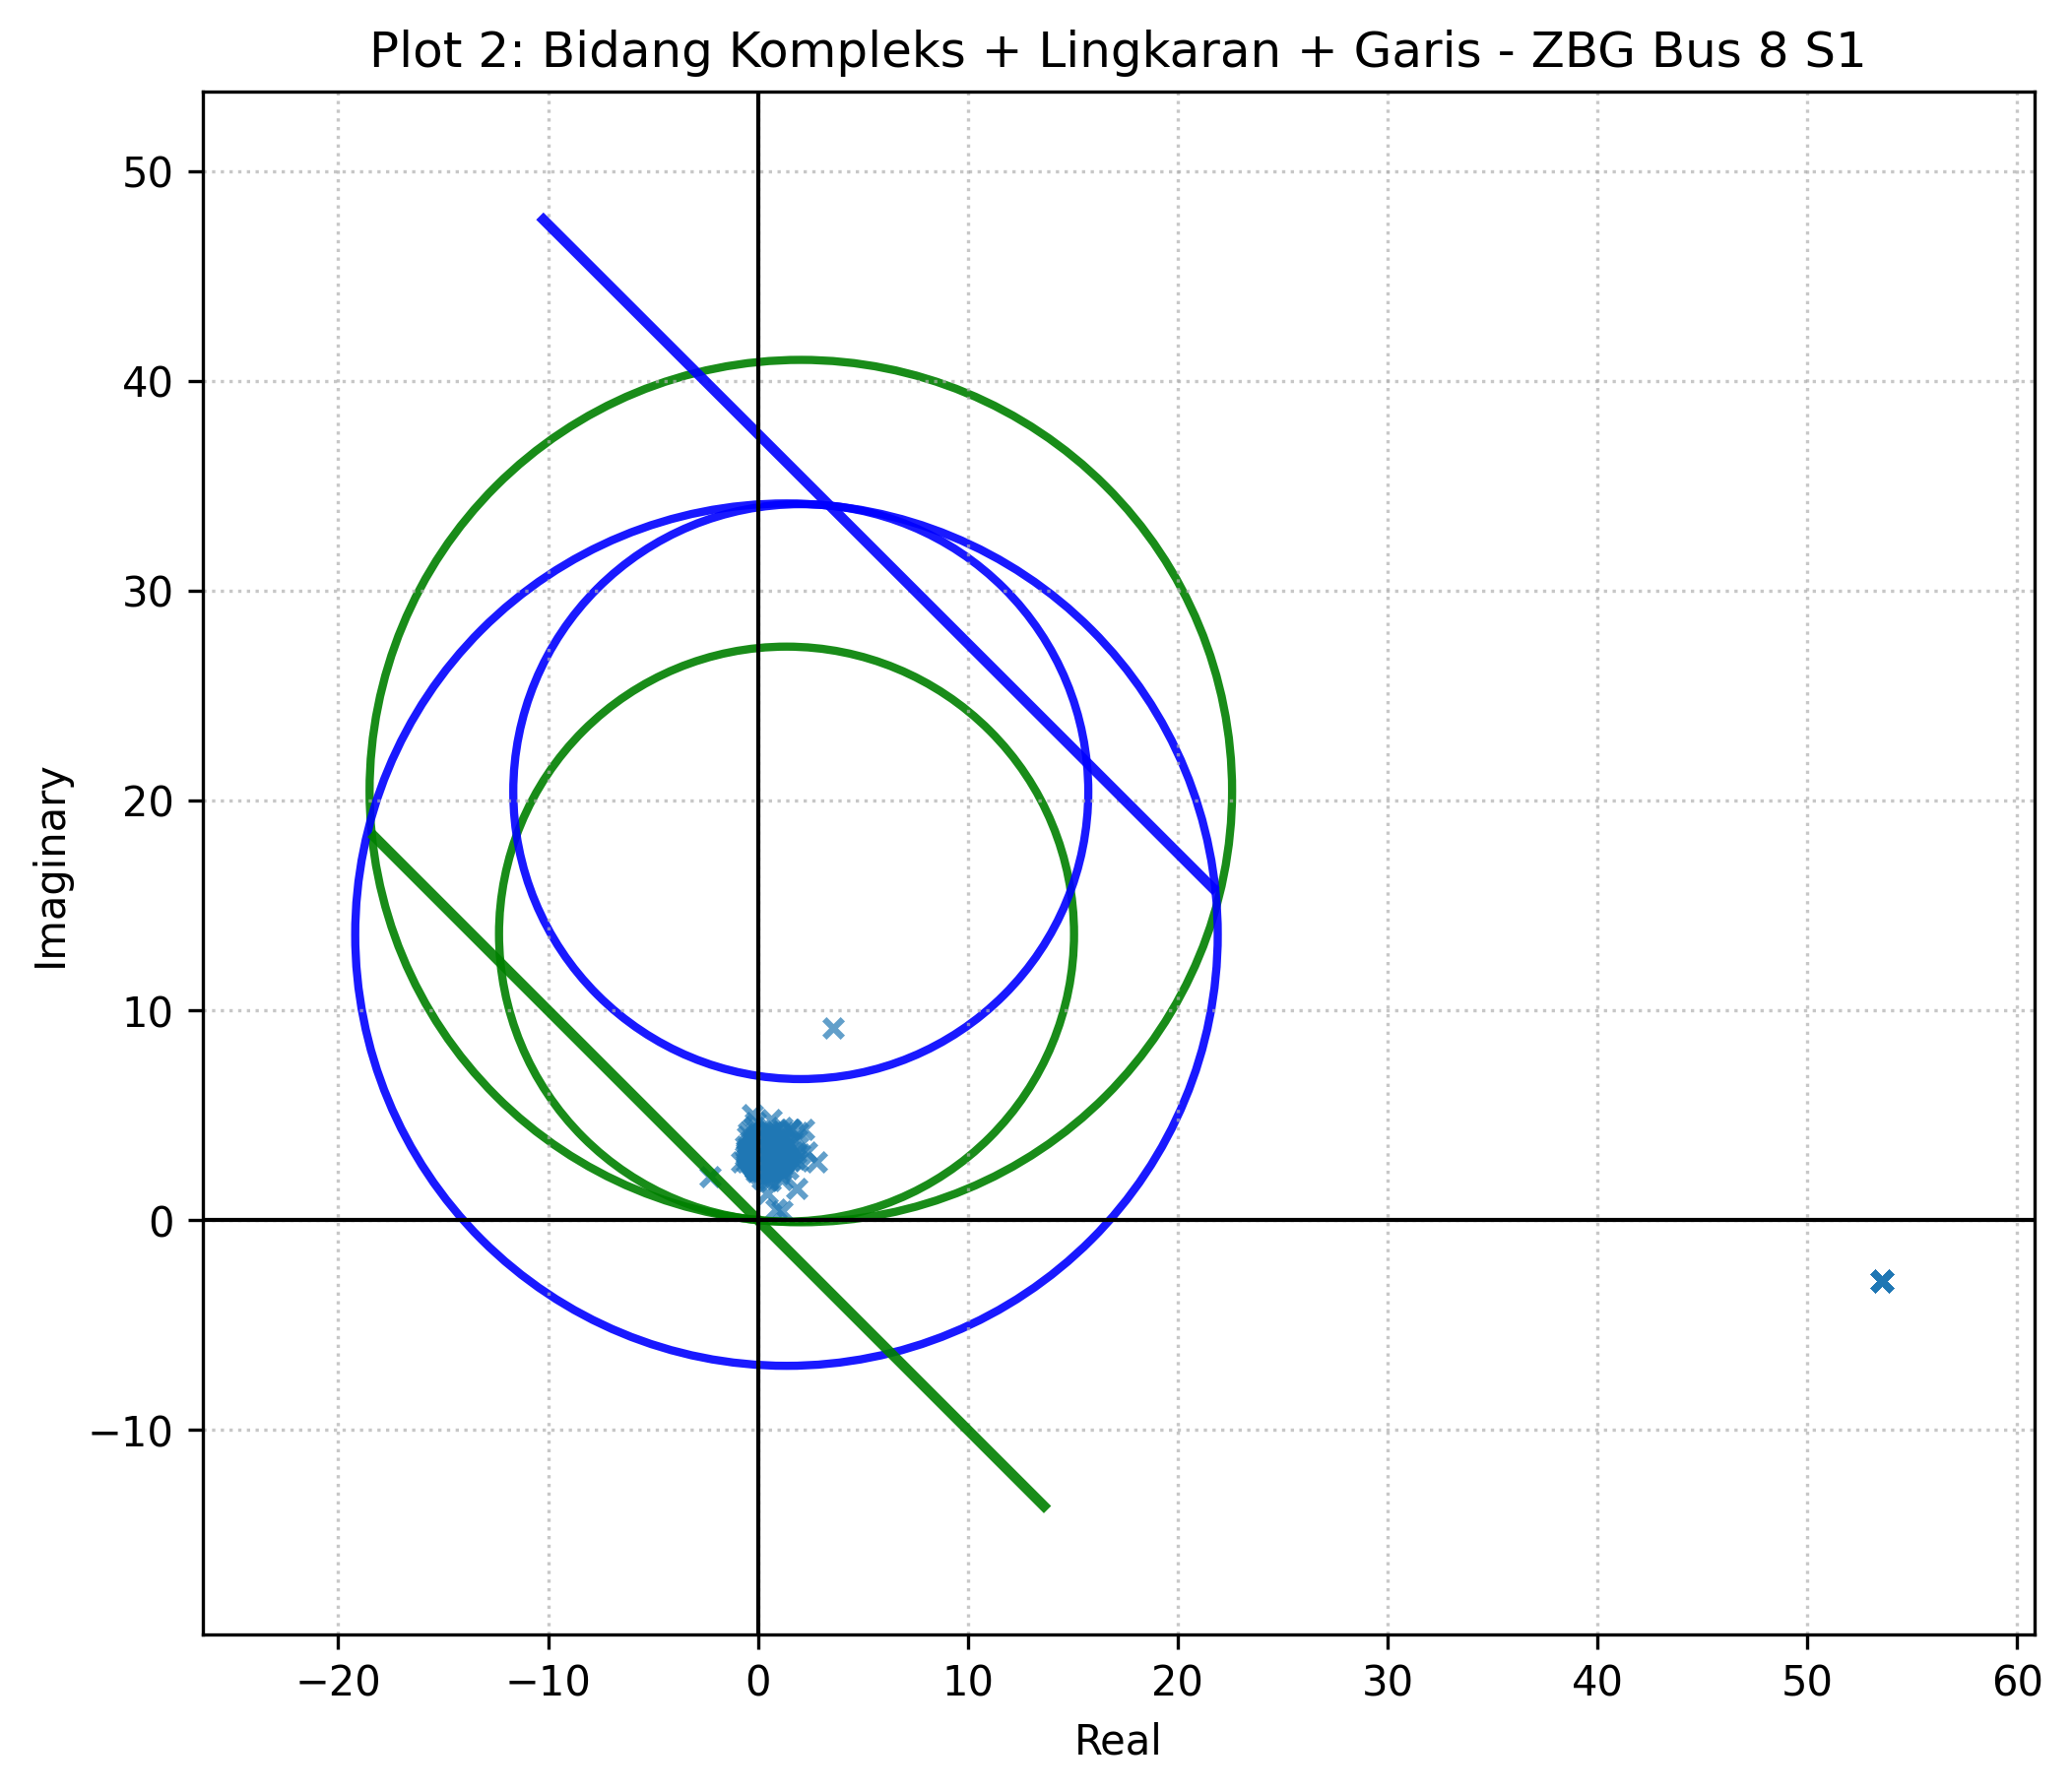
\includegraphics[width=0.8\textwidth]{contents/chapter-4/02_ZBG_Bus_8_S1_dengan_lingkaran_dan_garis.png}
%     \caption{Impedansi Tampak ZBG Bus 8 Skenario 1}
%     \label{fig:02_ZBG_Bus_8_S1_dengan_lingkaran_dan_garis}
% \end{figure}

% Pada gambar \ref{fig:02_ZBG_Bus_8_S1_dengan_lingkaran_dan_garis} terlihat untuk titik impedansi tampak pada fasa B dan ground terlihat cukup stabil dan relay 21 dari sisi bus 8 bekerja dengan normal sebagaimana mestinya dengan acuan pada \ref{subsec:tanpa_IBR_in_dlg} karena kontribusi dari sisi IBR tidak mendominasi karena TL78 tetap aktif mengakibatkan IBR tidak memengaruhi kinerja proteksi serta kontribusi tetap di dominasi oleh sistem tenaga konvensional.

%%%%%%%%%%%%%%%%%%%%%%%%%%%%%%%%%SISI PRIMER%%%%%%%%%%%%%%%%%%%%%%%%%%%%%%%%%%

% \begin{figure}[H]
%     \centering
%     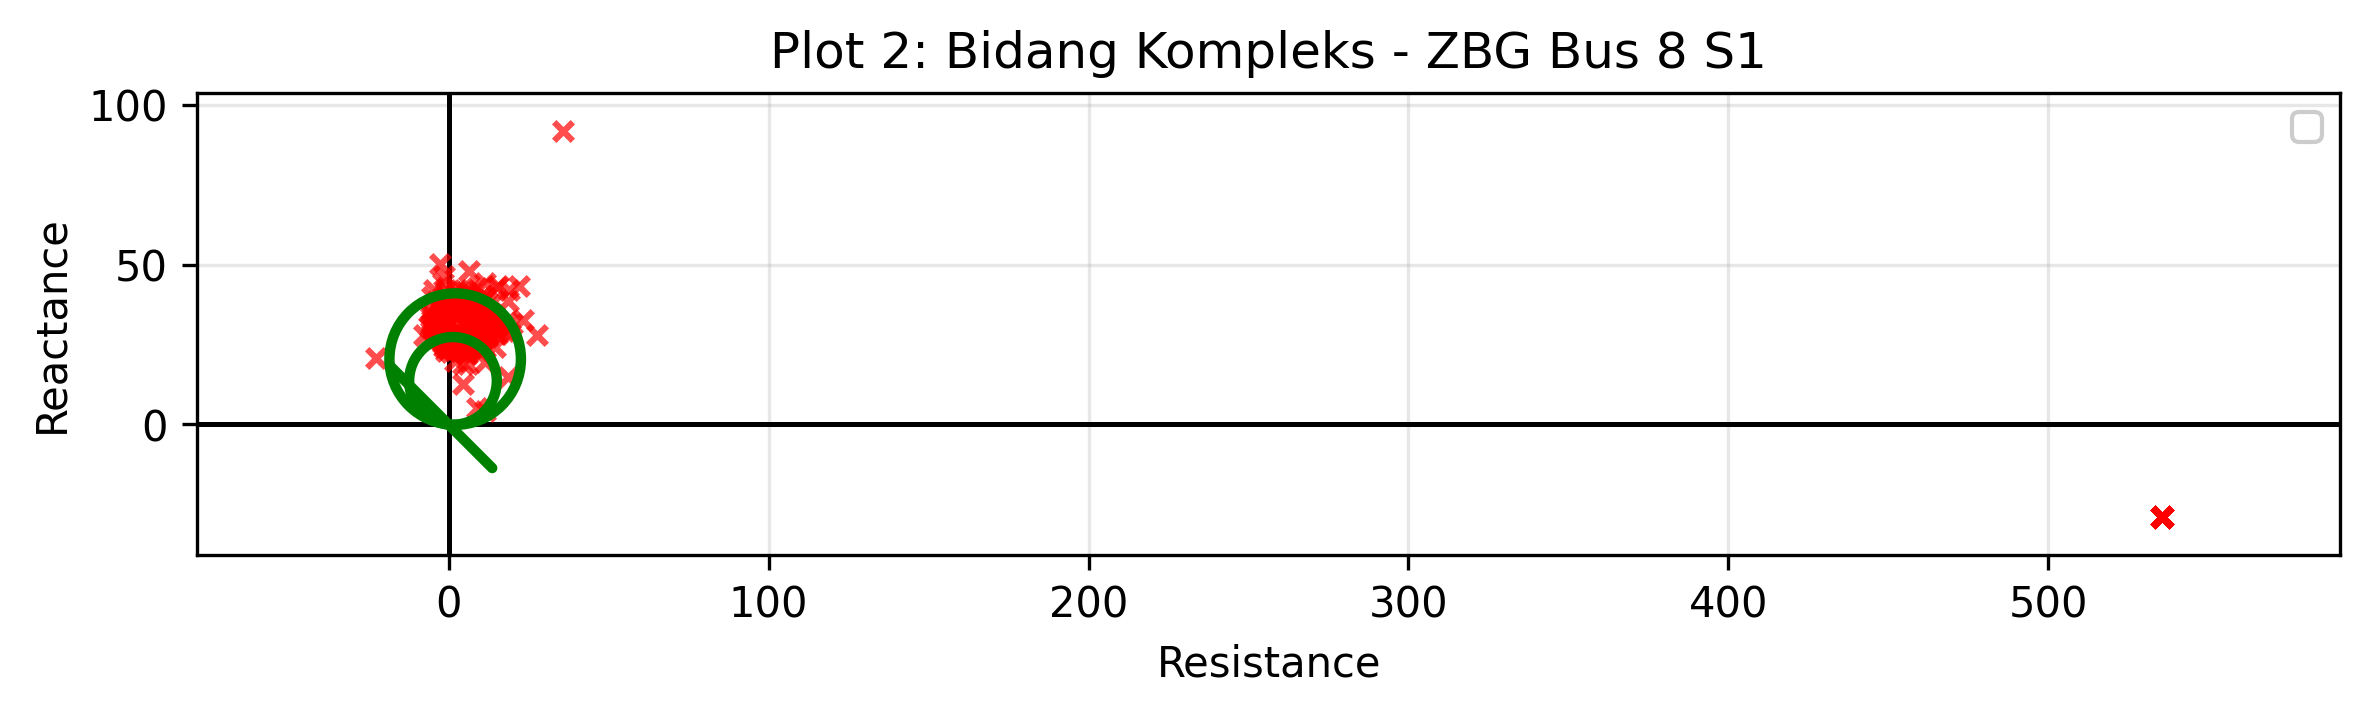
\includegraphics[width=0.8\textwidth]{contents/chapter-4/PRIA_02_ZBG_Bus_8_S1.png}
%     \caption{Impedansi Tampak ZBG Bus 8 Skenario 1}
%     \label{fig:PRIA_02_ZBG_Bus_8_S1}
% \end{figure}

% \begin{figure}[H]
%     \centering
%     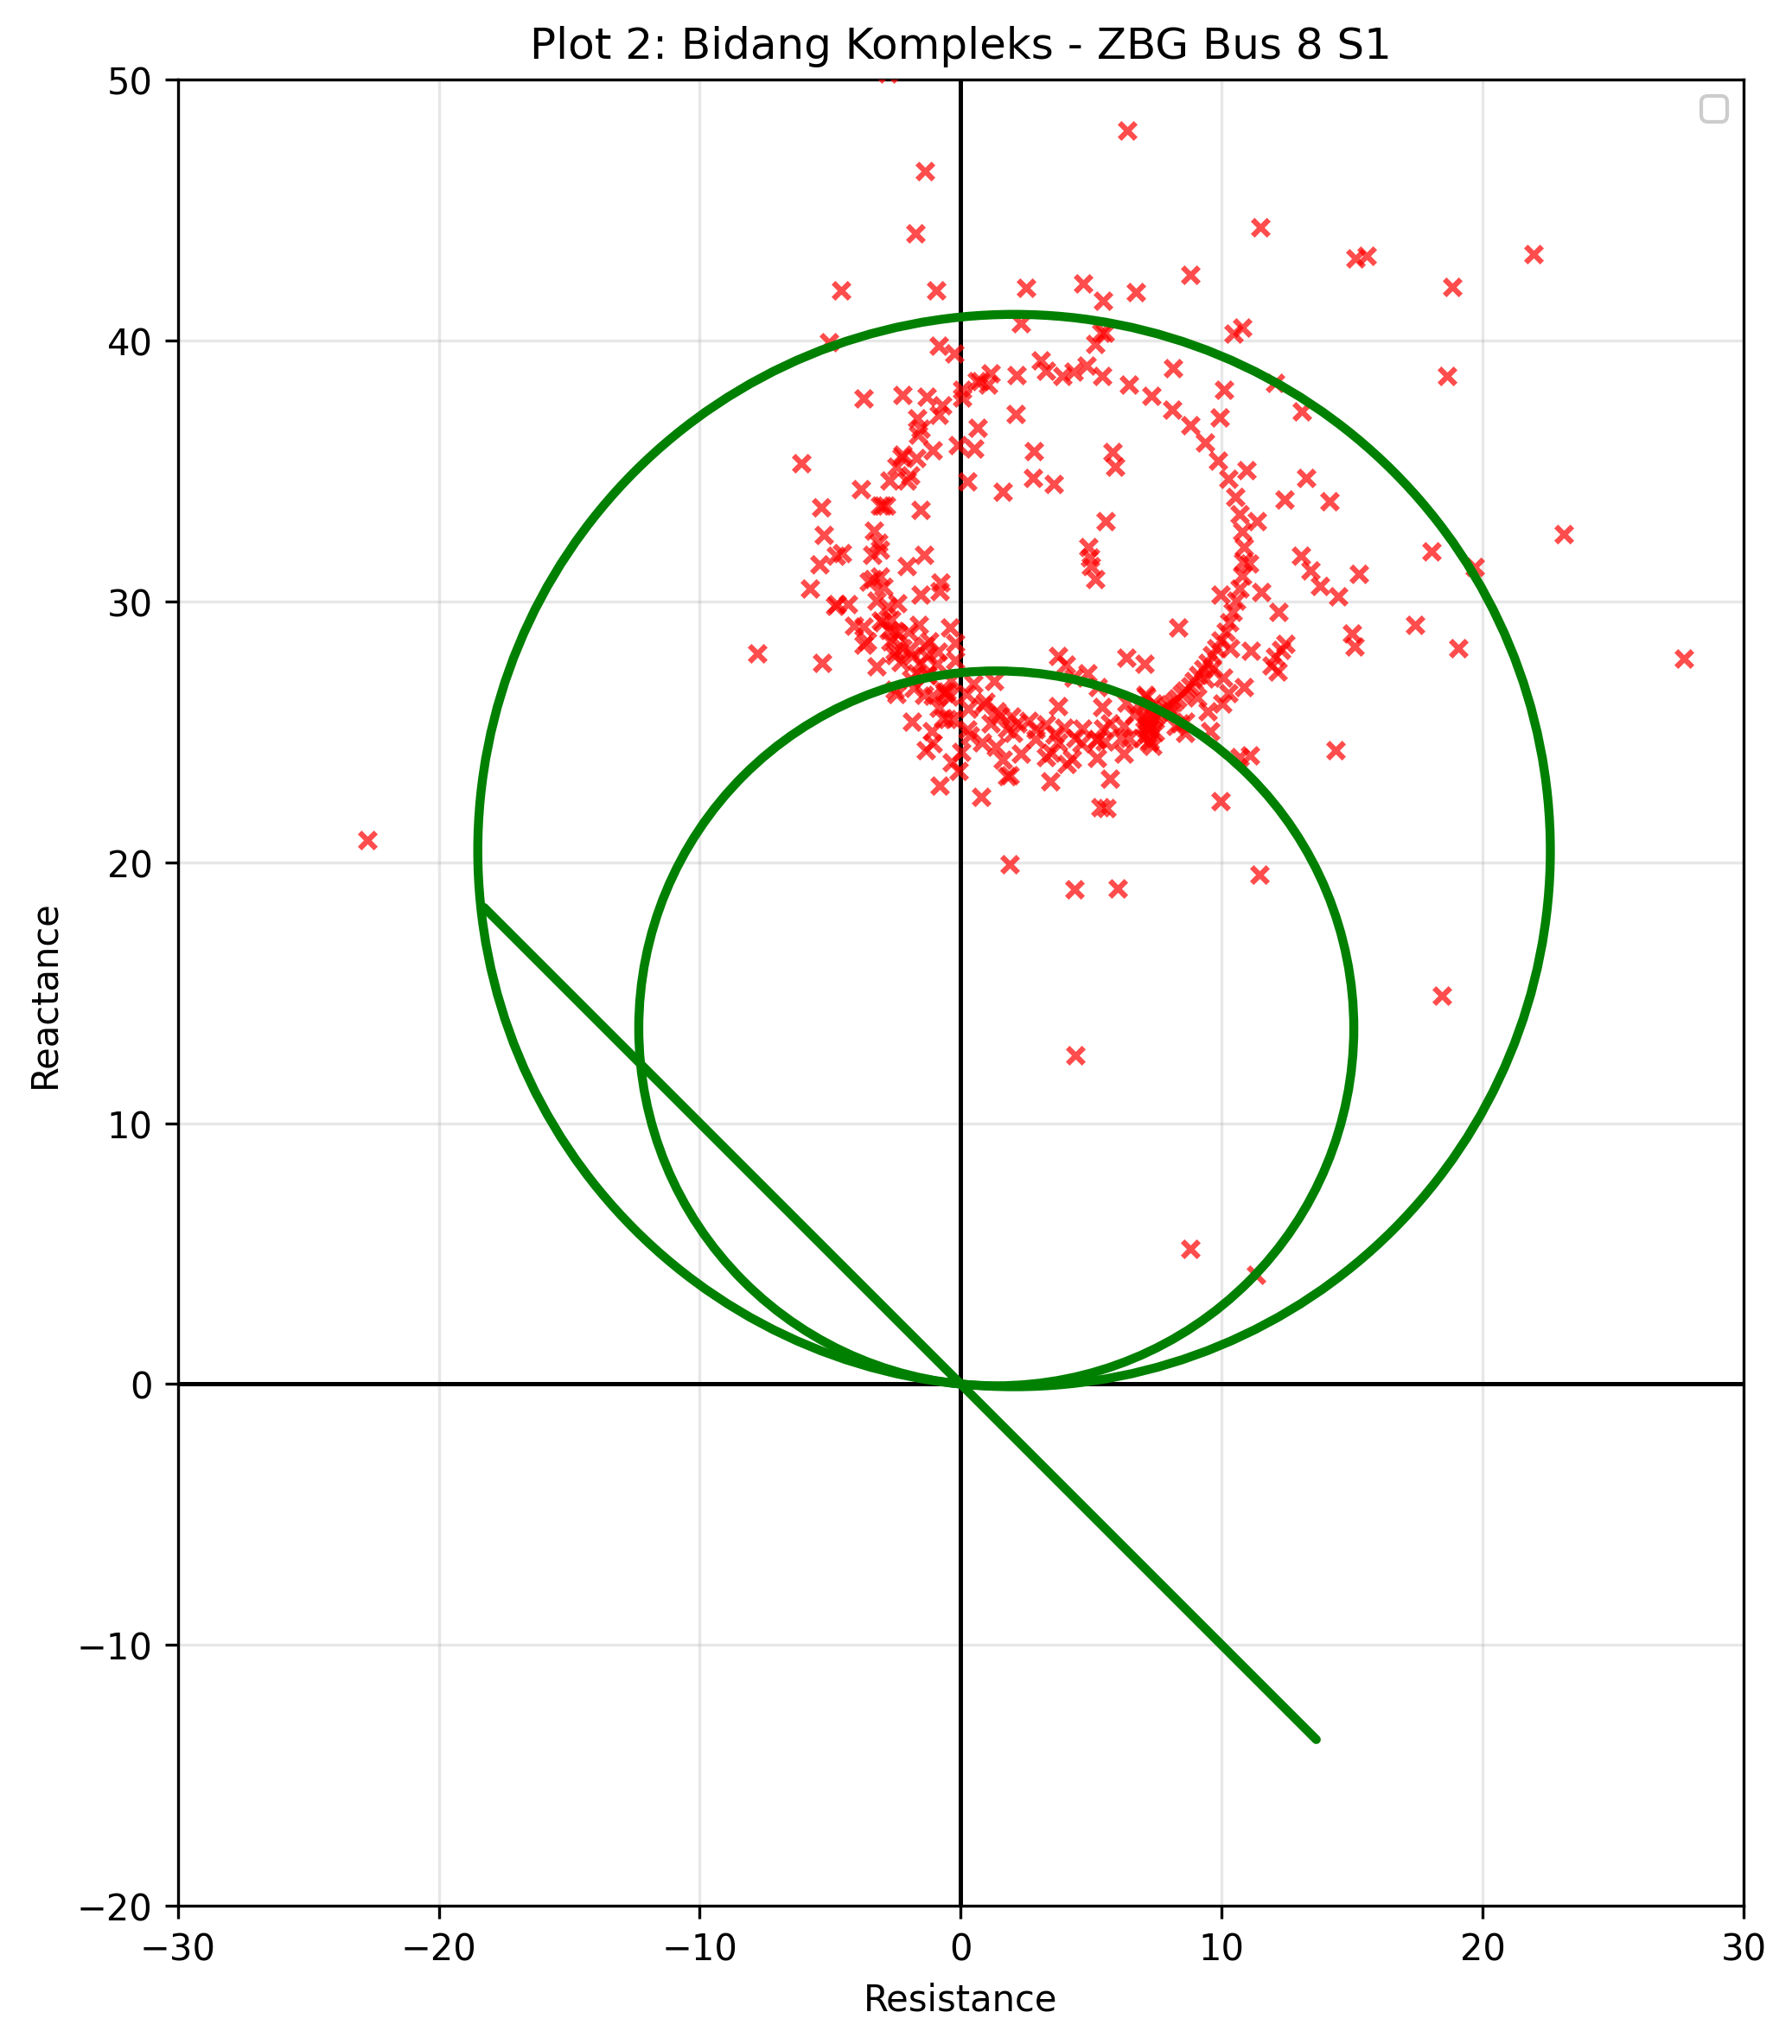
\includegraphics[width=0.8\textwidth]{contents/chapter-4/PRIZI_02_ZBG_Bus_8_S1.png}
%     \caption{Impedansi Tampak ZBG Bus 8 Skenario 1}
%     \label{fig:PRIZI_02_ZBG_Bus_8_S1}
% \end{figure}

\begin{figure}[H]
    \centering

    % Gambar sebelah kiri
    \begin{subfigure}[t]{0.48\textwidth}
        \centering
        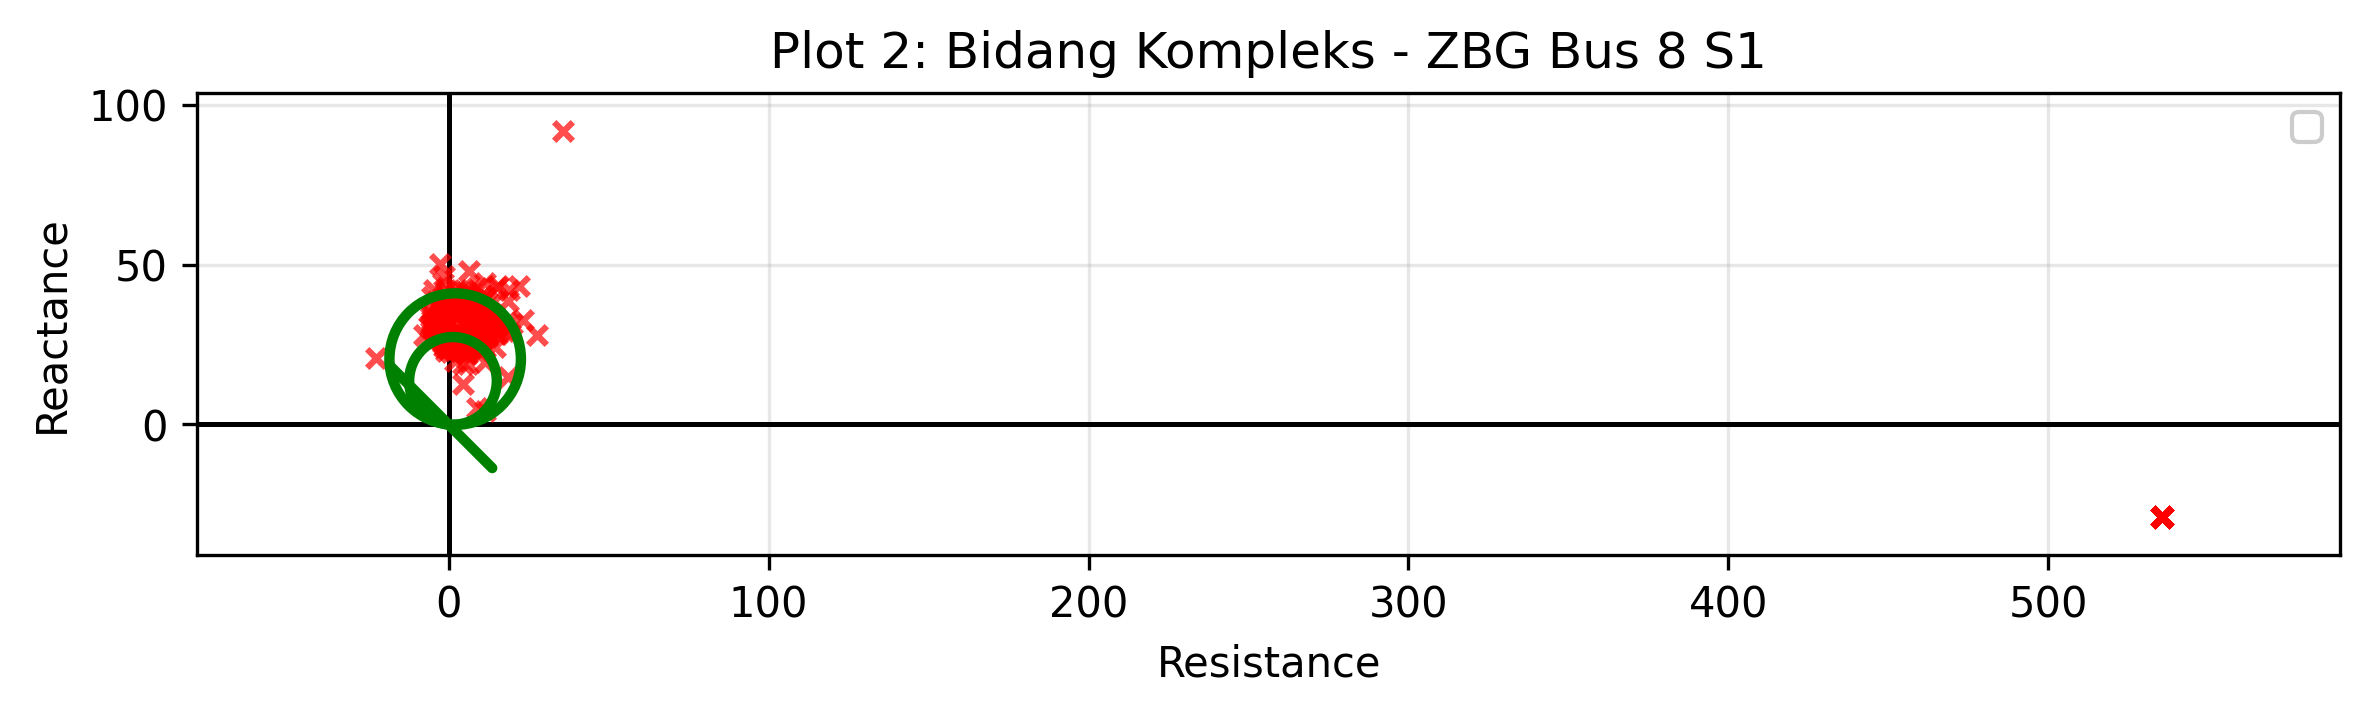
\includegraphics[width=\textwidth]{contents/chapter-4/PRIA_02_ZBG_Bus_8_S1.png}
        \caption{Seluruh Impedansi Tampak}
        \label{fig:PRIA_02_ZBG_Bus_8_S1}
    \end{subfigure}
    \hfill
    % Gambar sebelah kanan
    \begin{subfigure}[t]{0.48\textwidth}
        \centering
        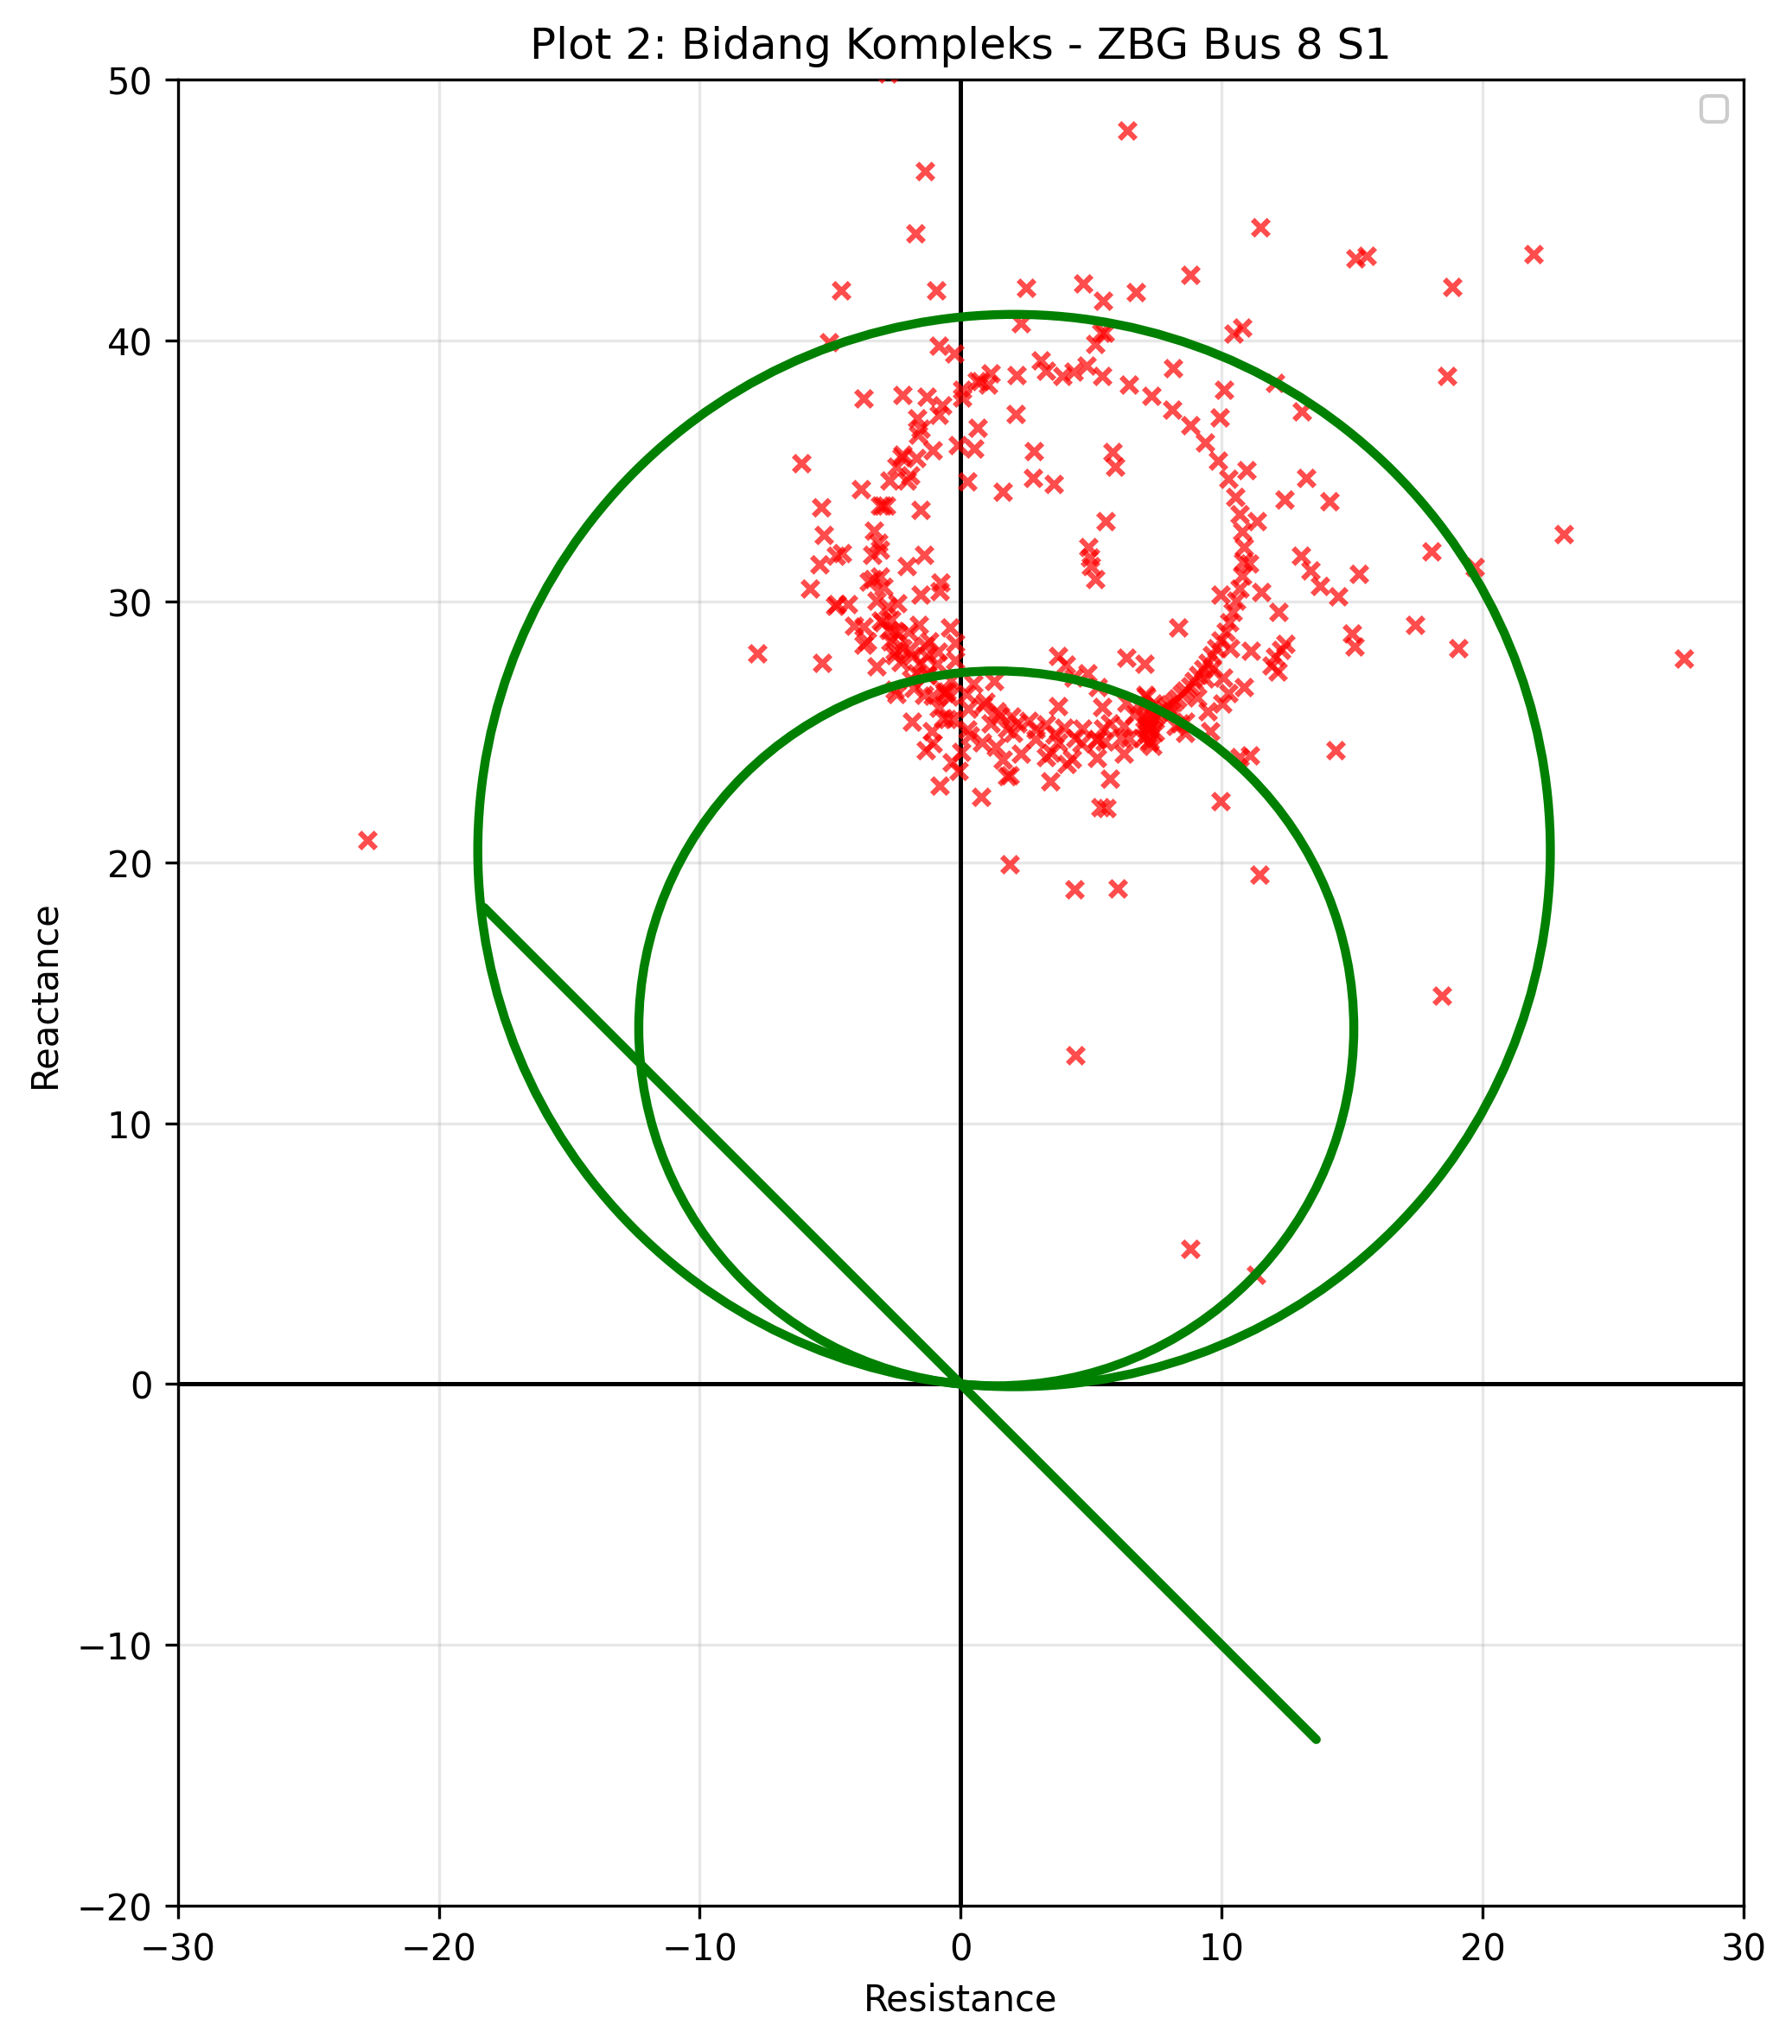
\includegraphics[width=\textwidth]{contents/chapter-4/PRIZI_02_ZBG_Bus_8_S1.png}
        \caption{Zoom In Pada Zona Proteksi}
        \label{fig:PRIZI_02_ZBG_Bus_8_S1}
    \end{subfigure}

    \caption{Impedansi Tampak ZBG Bus 8 Skenario 1}
    \label{fig:Impedansi_Tampak_ZBG_Bus_8_S1}
\end{figure}

Pada gambar \ref{fig:Impedansi_Tampak_ZBG_Bus_8_S1} terlihat untuk titik impedansi tampak pada fasa B dan ground yang dibaca oleh relay 21 dari sisi bus 8 bekerja dengan baik sebagaimana mestinya dengan acuan pada \ref{subsec:tanpa_IBR_in_dlg} karena kontribusi dari sisi IBR tidak mendominasi karena TL78 tetap aktif mengakibatkan IBR tidak memengaruhi kinerja proteksi serta kontribusi tetap di dominasi oleh sistem tenaga konvensional.

%%%%%%%%%%%%%%%%%%%%%%%%%%%%%%%%%%%%%%%%%%%%%%%%%%%%%%%%%%%%%%%

% \begin{figure}[H]
%     \centering
%     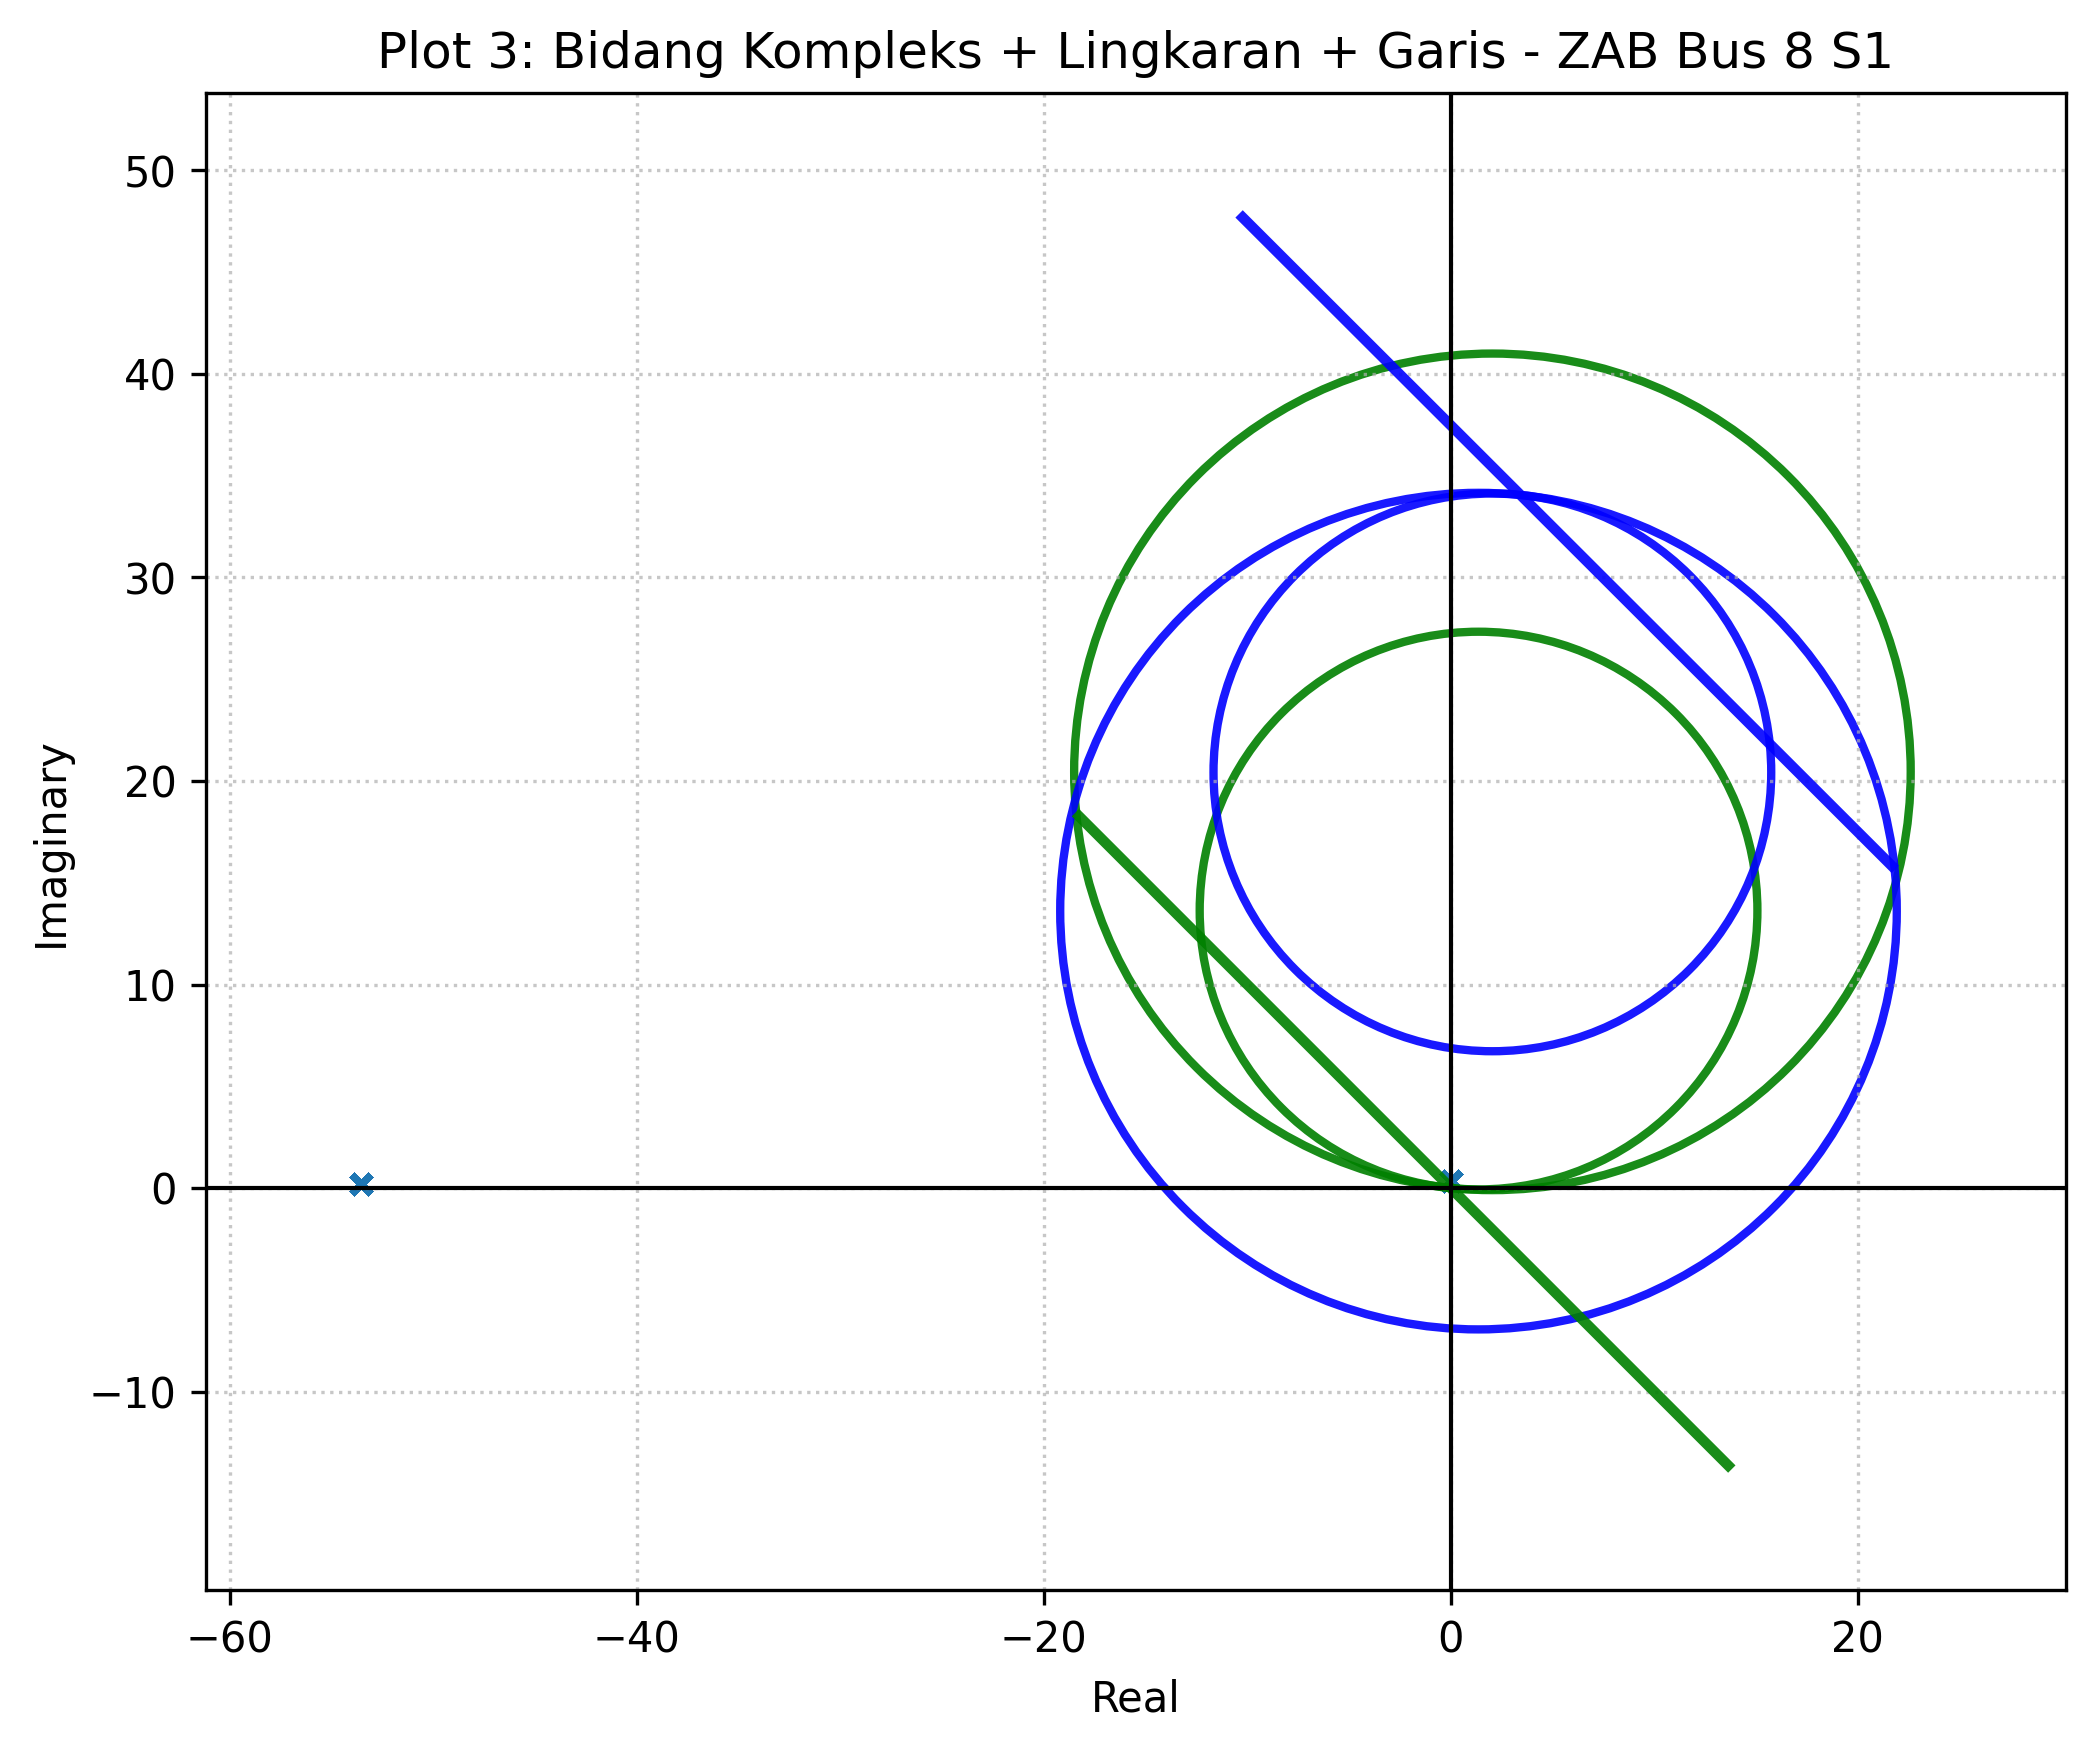
\includegraphics[width=0.8\textwidth]{contents/chapter-4/03_ZAB_Bus_8_S1_dengan_lingkaran_dan_garis.png}
%     \caption{Impedansi Tampak ZAB Bus 8 Skenario 1}
%     \label{fig:03_ZAB_Bus_8_S1_dengan_lingkaran_dan_garis}
% \end{figure}

% Pada gambar \ref{fig:03_ZAB_Bus_8_S1_dengan_lingkaran_dan_garis} terlihat untuk titik impedansi tampak pada fasa A dan fasa B terlihat cukup stabil dan relay 21 dari sisi bus 8 bekerja dengan normal sebagaimana mestinya dengan acuan pada \ref{subsec:tanpa_IBR_in_dlg} karena kontribusi dari sisi IBR tidak mendominasi karena TL78 tetap aktif mengakibatkan IBR tidak memengaruhi kinerja proteksi serta kontribusi tetap di dominasi oleh sistem tenaga konvensional.

%%%%%%%%%%%%%%%%%%%%%%%%%%%%%%%%%SISI PRIMER%%%%%%%%%%%%%%%%%%%%%%%%%%%%%%%%%%

% \begin{figure}[H]
%     \centering
%     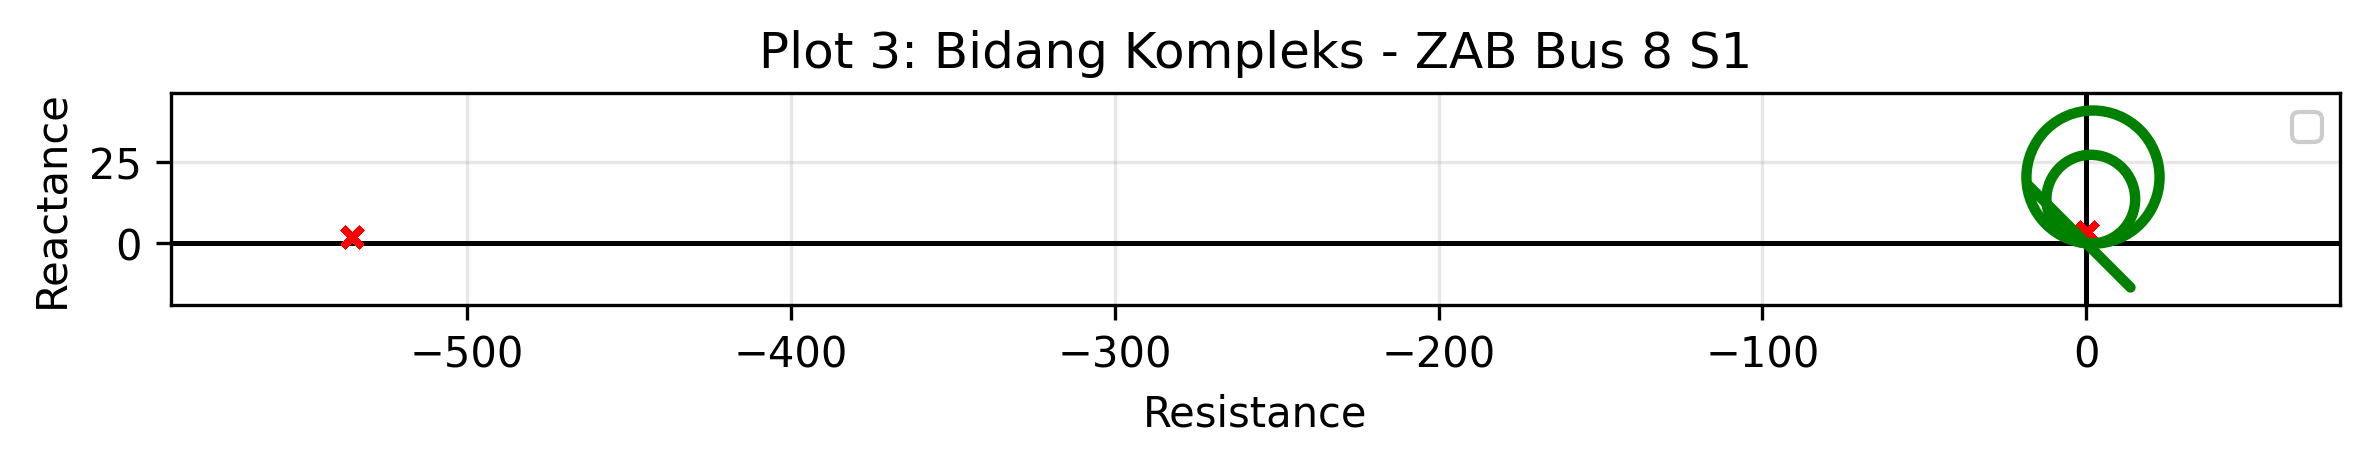
\includegraphics[width=0.8\textwidth]{contents/chapter-4/PRIA_03_ZAB_Bus_8_S1.png}
%     \caption{Impedansi Tampak ZAB Bus 8 Skenario 1}
%     \label{fig:PRIA_03_ZAB_Bus_8_S1}
% \end{figure}

% \begin{figure}[H]
%     \centering
%     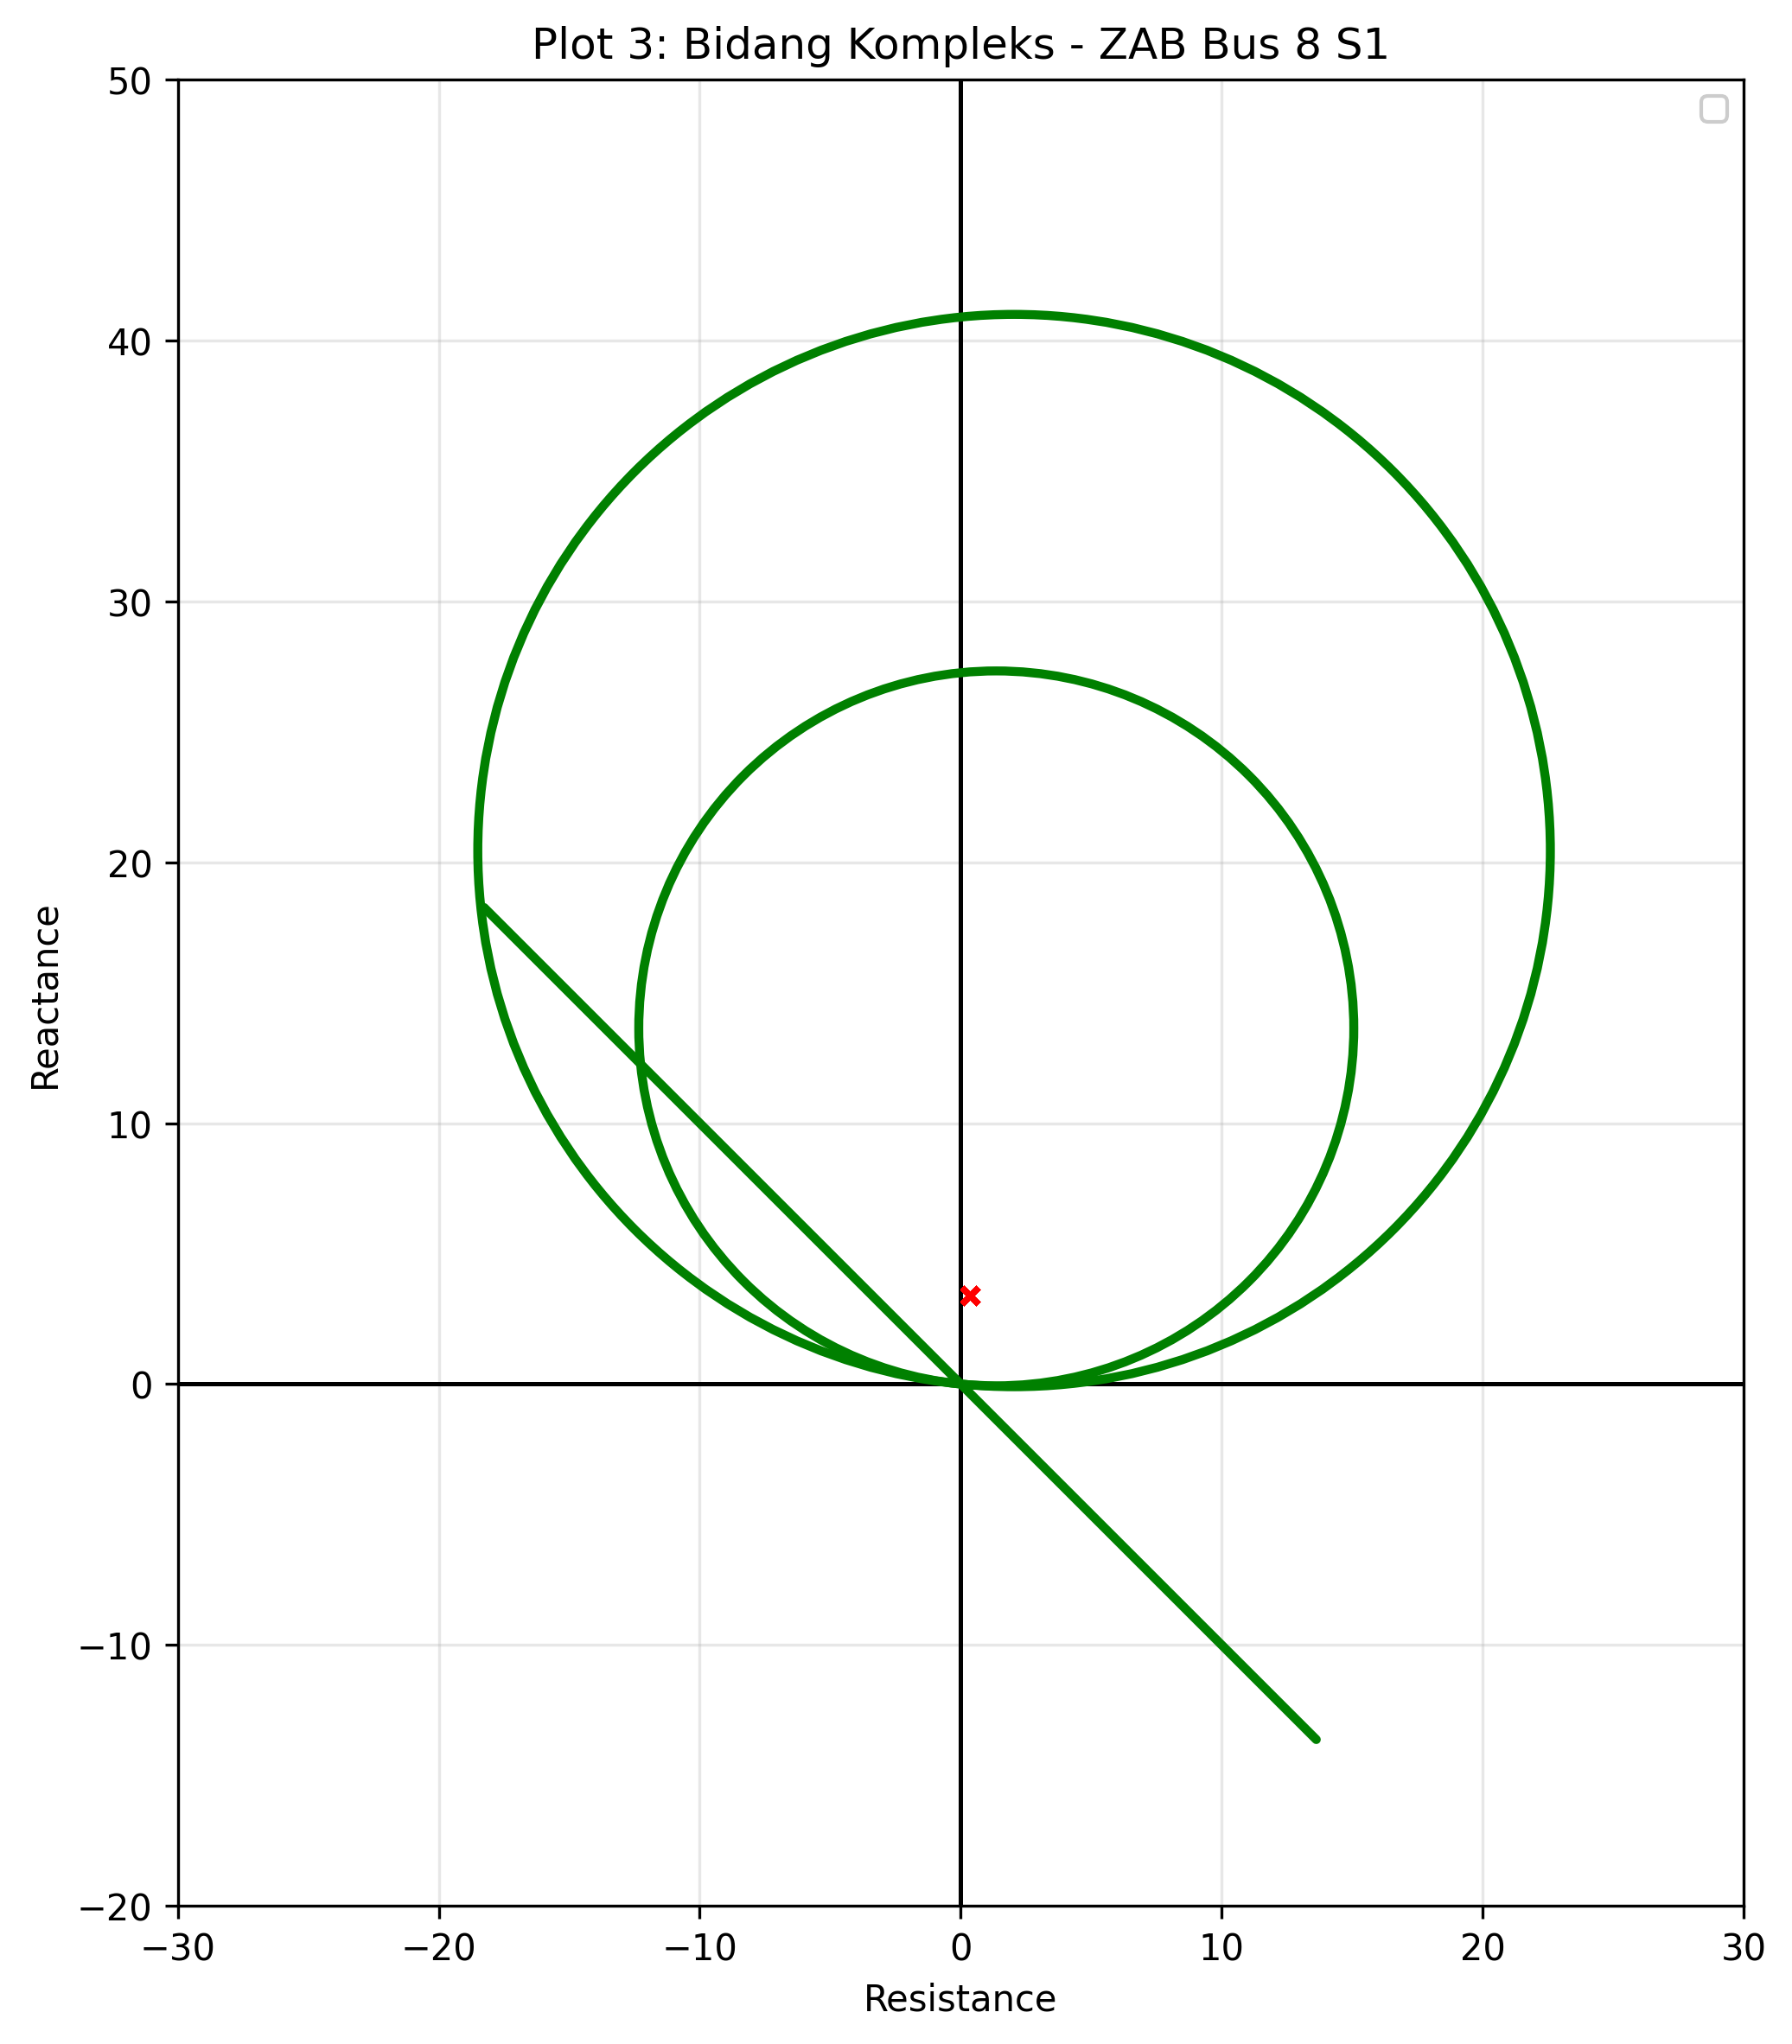
\includegraphics[width=0.8\textwidth]{contents/chapter-4/PRIZI_03_ZAB_Bus_8_S1.png}
%     \caption{Impedansi Tampak ZAB Bus 8 Skenario 1}
%     \label{fig:PRIZI_03_ZAB_Bus_8_S1}
% \end{figure}

\begin{figure}[H]
    \centering

    % Gambar sebelah kiri
    \begin{subfigure}[t]{0.48\textwidth}
        \centering
        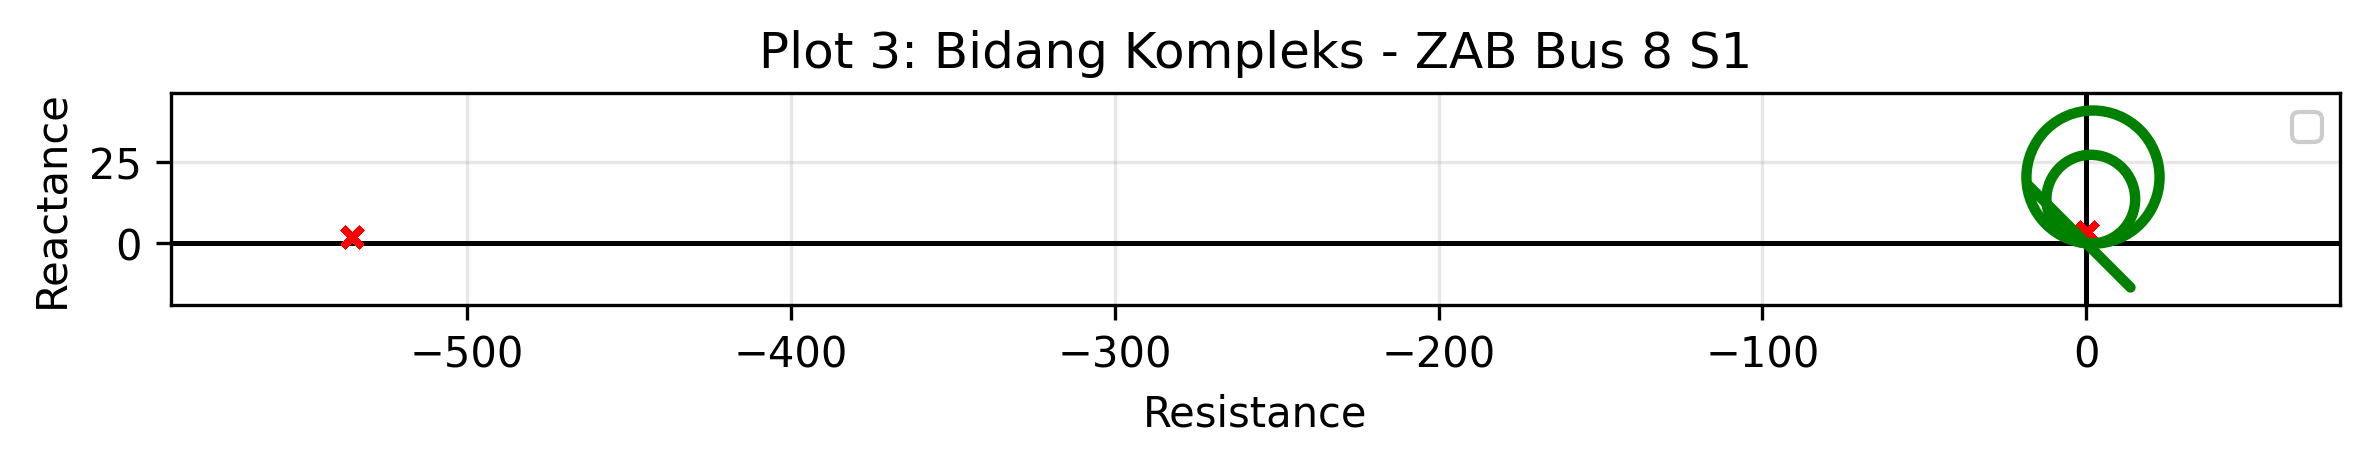
\includegraphics[width=\textwidth]{contents/chapter-4/PRIA_03_ZAB_Bus_8_S1.png}
        \caption{Seluruh Impedansi Tampak}
        \label{fig:PRIA_03_ZAB_Bus_8_S1}
    \end{subfigure}
    \hfill
    % Gambar sebelah kanan
    \begin{subfigure}[t]{0.48\textwidth}
        \centering
        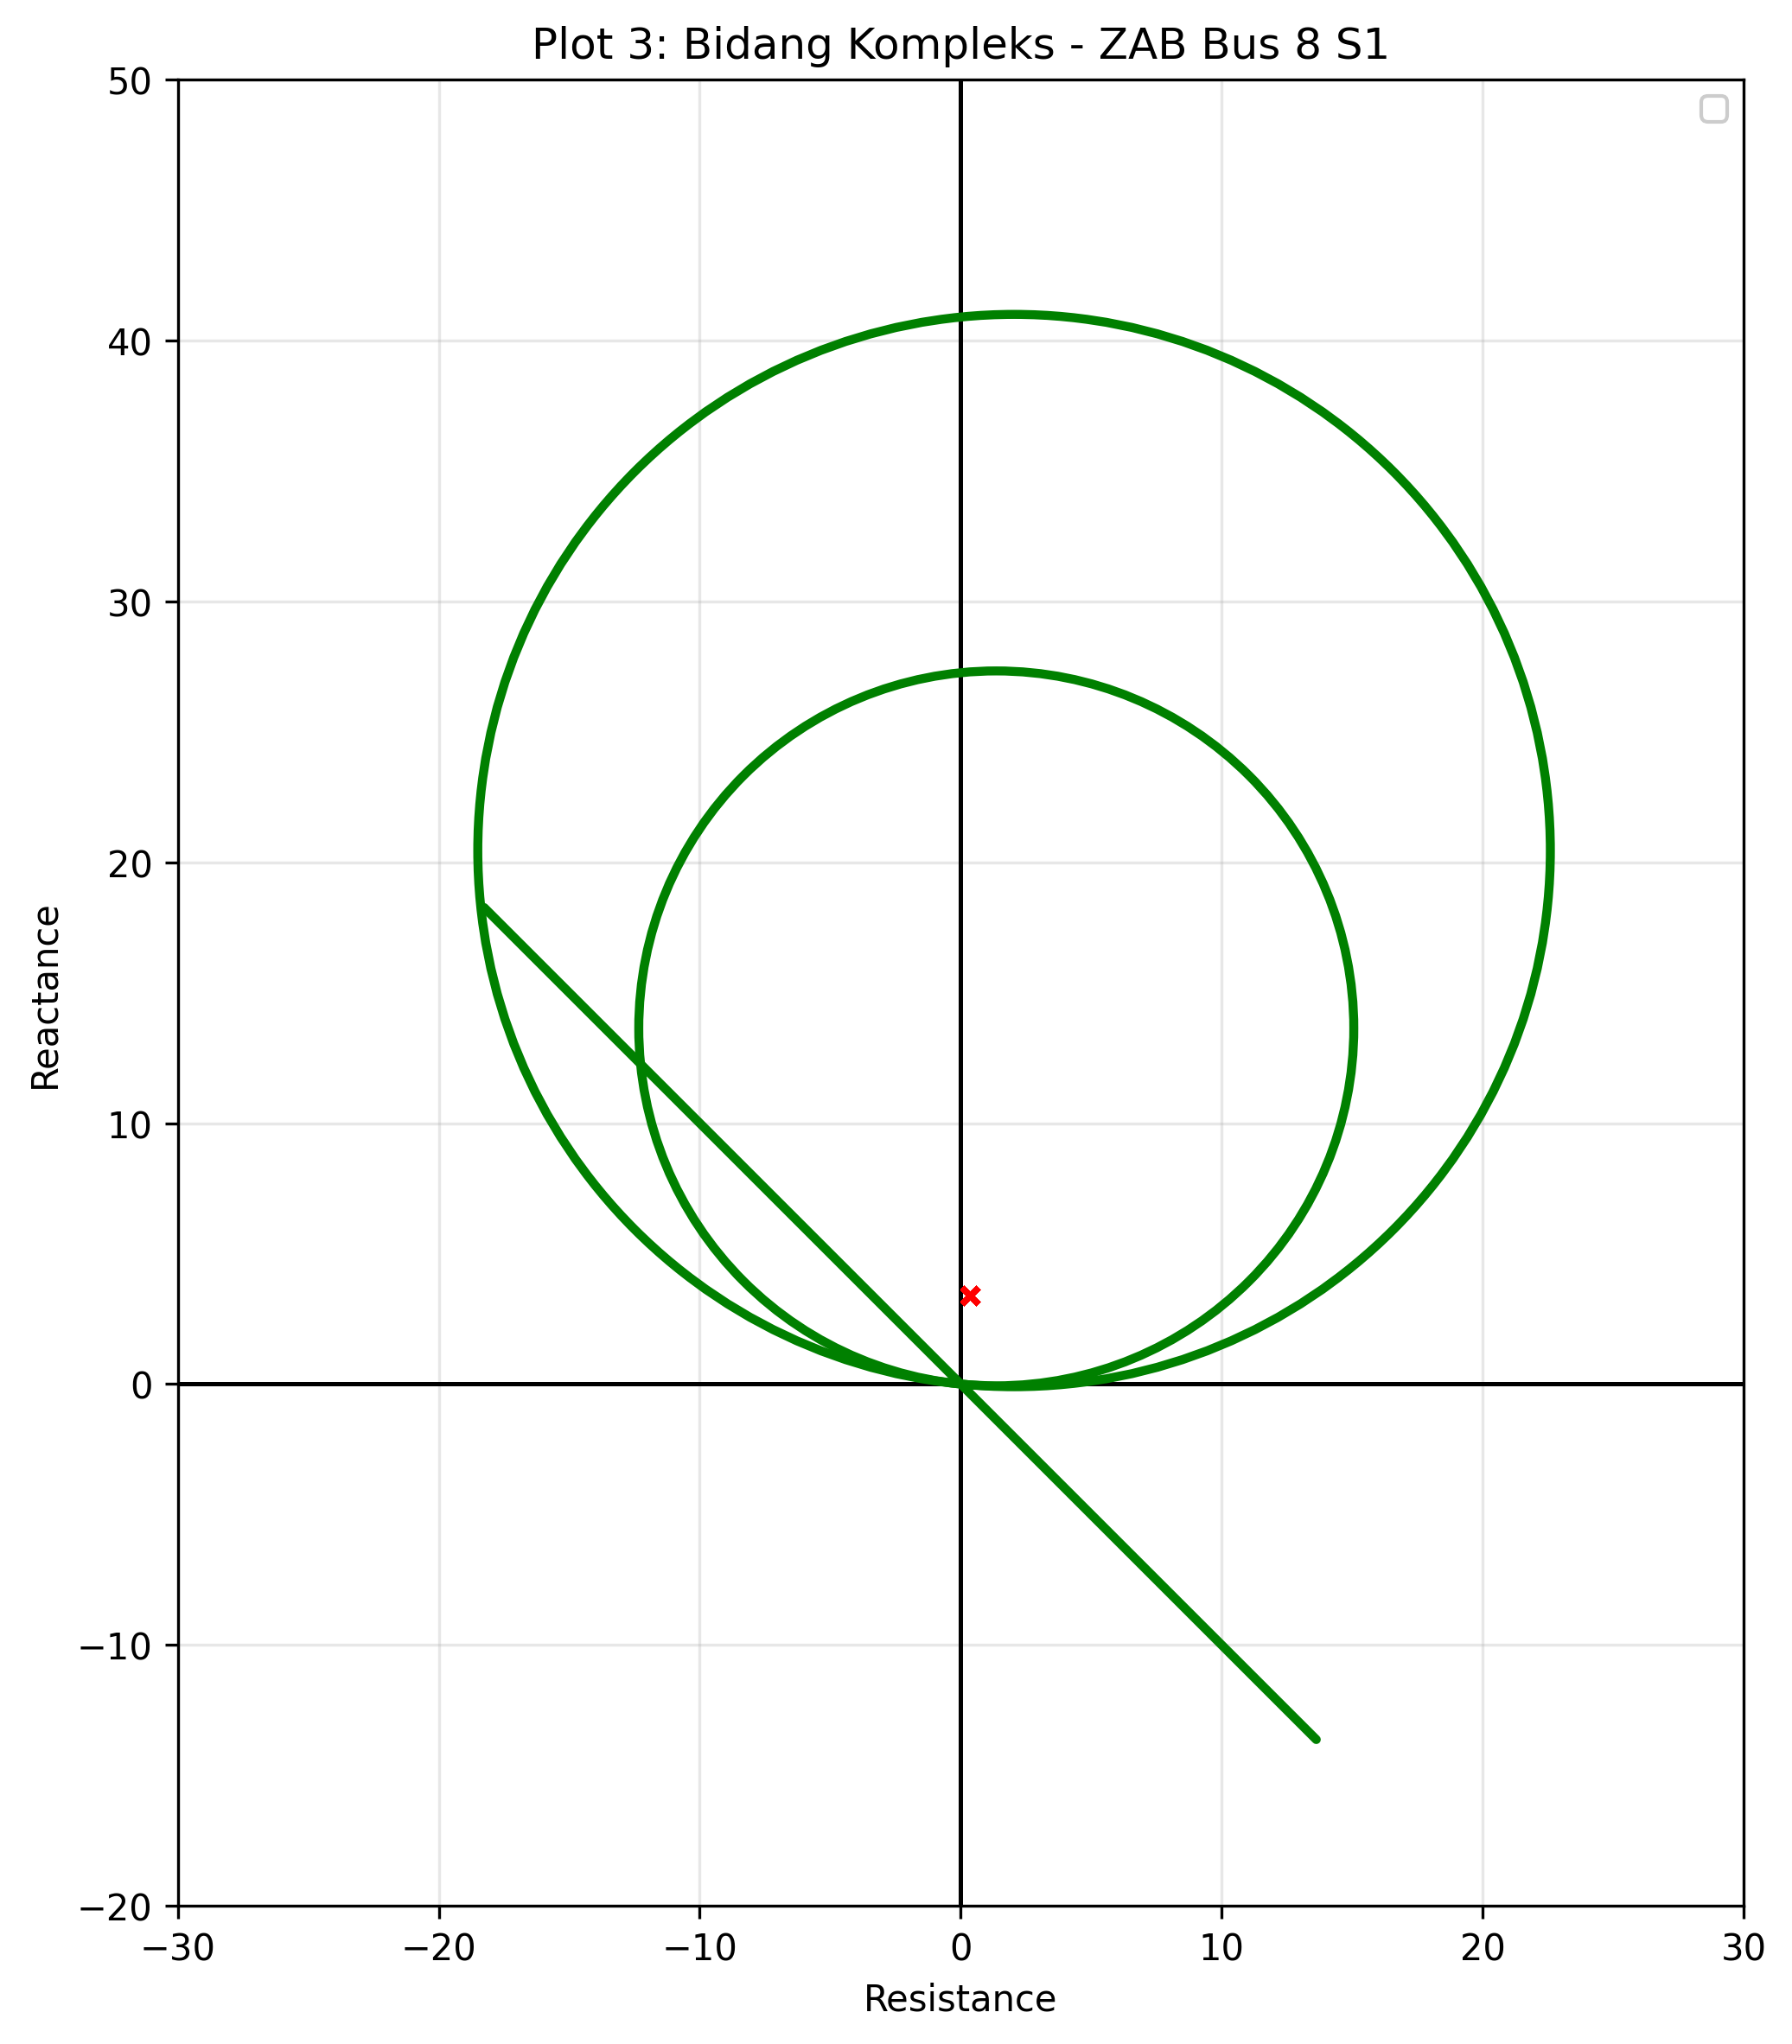
\includegraphics[width=\textwidth]{contents/chapter-4/PRIZI_03_ZAB_Bus_8_S1.png}
        \caption{Zoom In Pada Zona Proteksi}
        \label{fig:PRIZI_03_ZAB_Bus_8_S1}
    \end{subfigure}

    \caption{Impedansi Tampak ZAB Bus 8 Skenario 1}
    \label{fig:Impedansi_Tampak_ZAB_Bus_8_S1}
\end{figure}

Pada gambar \ref{fig:Impedansi_Tampak_ZAB_Bus_8_S1} terlihat untuk titik impedansi tampak pada fasa A dan fasa B terlihat cukup stabil dan relay 21 dari sisi bus 8 bekerja dengan baik sebagaimana mestinya dengan acuan pada \ref{subsec:tanpa_IBR_in_dlg} karena kontribusi dari sisi IBR tidak mendominasi karena TL78 tetap aktif mengakibatkan IBR tidak memengaruhi kinerja proteksi serta kontribusi tetap di dominasi oleh sistem tenaga konvensional. Walaupun impedansi loop fasa A dan B terbaca pada zona 1 namun relay tetap trip pada zona 2 dikarenakan melihat pada impedansi loop yang lainnya.

%%%%%%%%%%%%%%%%%%%%%%%%%%%%%%%%%%%%%%%%%%%%%%%%%%%%%%%%%%%%%%%

% \begin{figure}[H]
%     \centering
%     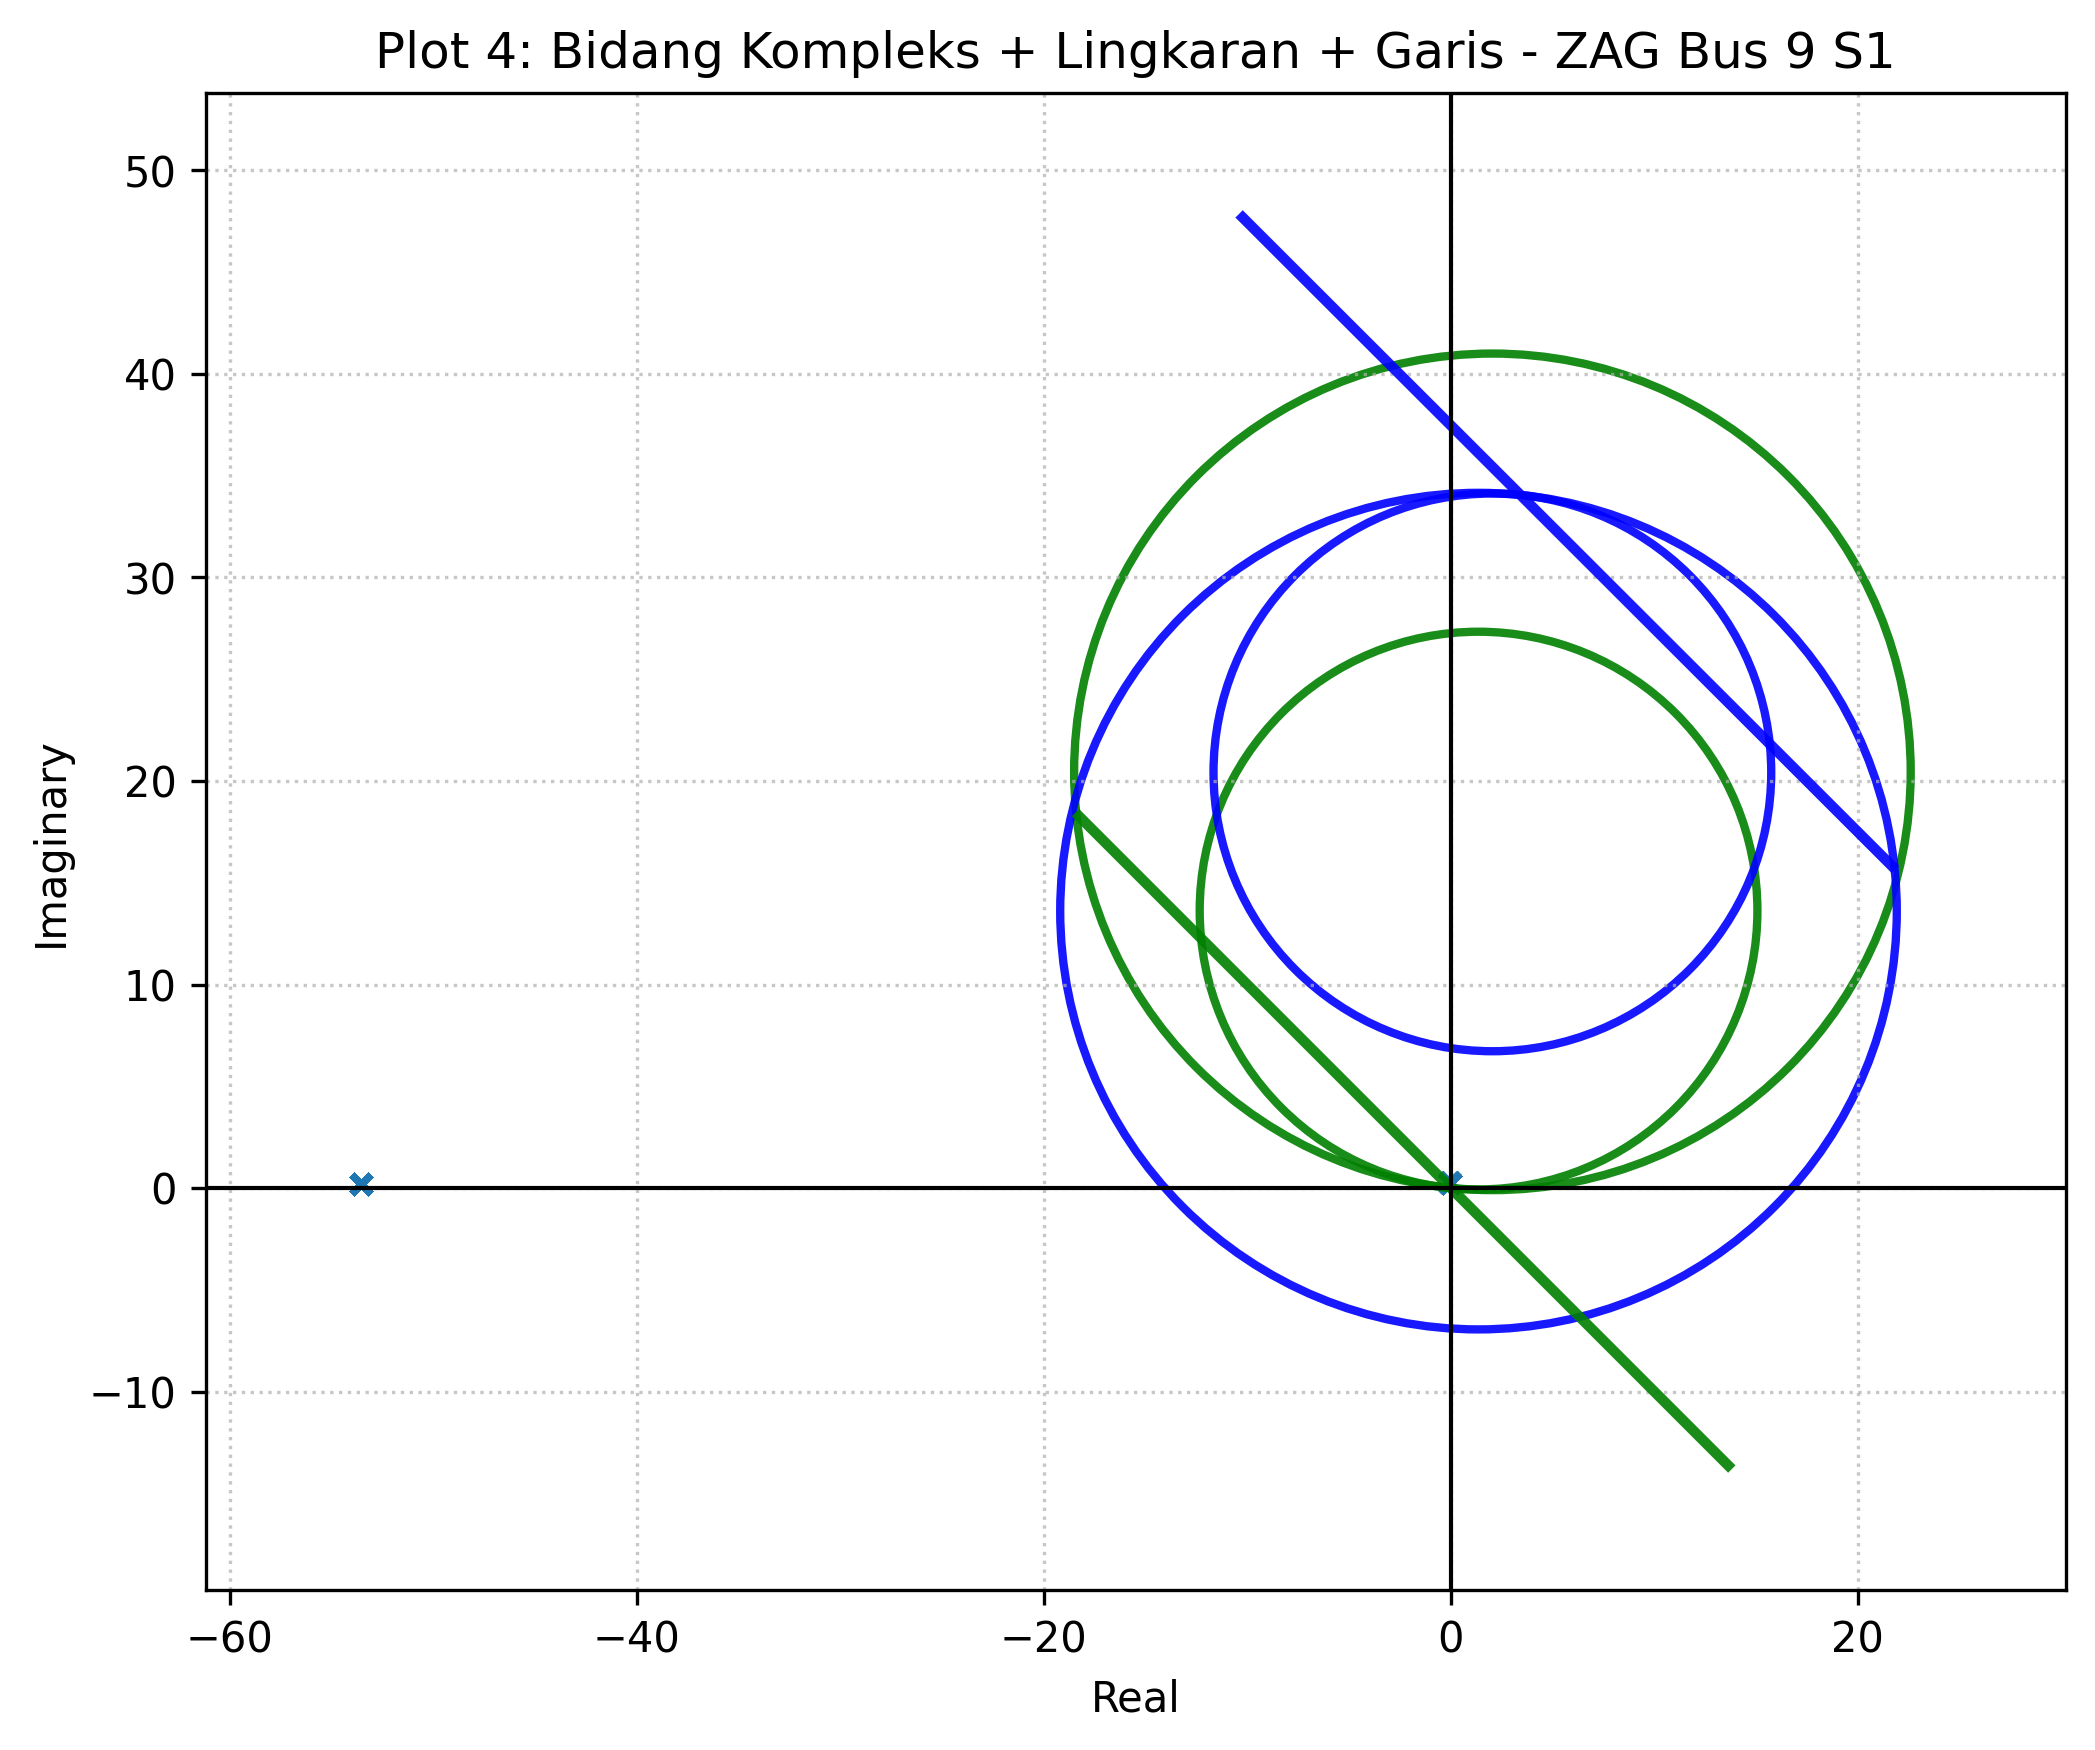
\includegraphics[width=0.8\textwidth]{contents/chapter-4/04_ZAG_Bus_9_S1_dengan_lingkaran_dan_garis.png}
%     \caption{Impedansi Tampak ZAG Bus 9 Skenario 1}
%     \label{fig:04_ZAG_Bus_9_S1_dengan_lingkaran_dan_garis}
% \end{figure}

% Pada gambar \ref{fig:04_ZAG_Bus_9_S1_dengan_lingkaran_dan_garis} terlihat untuk titik impedansi tampak pada fasa A dan ground terlihat cukup stabil dan relay 21 dari sisi bus 9 bekerja dengan normal sebagaimana mestinya dengan acuan pada \ref{subsec:tanpa_IBR_in_dlg} karena kontribusi dari sisi IBR tidak mendominasi karena TL78 tetap aktif mengakibatkan IBR tidak memengaruhi kinerja proteksi serta kontribusi tetap di dominasi oleh sistem tenaga konvensional.

%%%%%%%%%%%%%%%%%%%%%%%%%%%%%%%%%SISI PRIMER%%%%%%%%%%%%%%%%%%%%%%%%%%%%%%%%%%

% \begin{figure}[H]
%     \centering
%     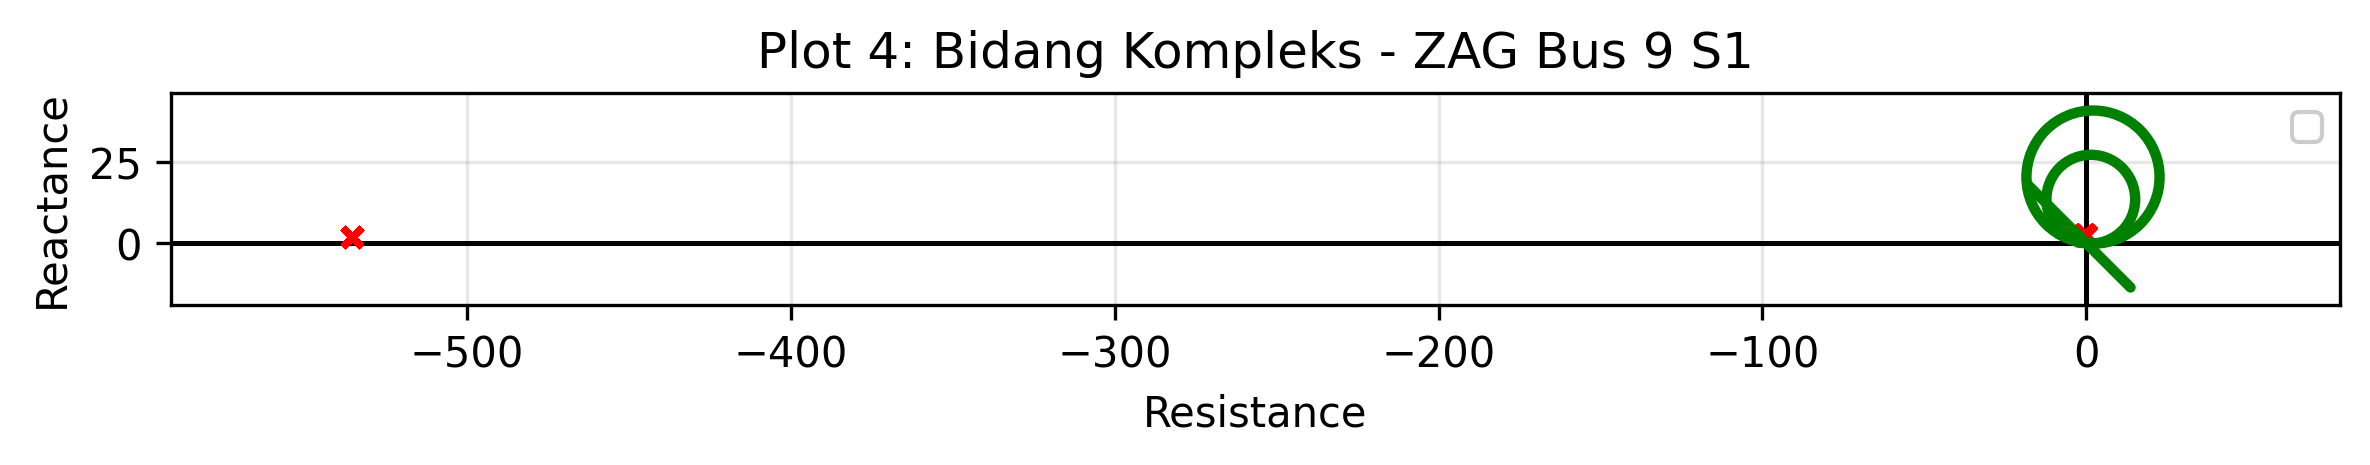
\includegraphics[width=0.8\textwidth]{contents/chapter-4/PRIA_04_ZAG_Bus_9_S1.png}
%     \caption{Impedansi Tampak ZAG Bus 9 Skenario 1}
%     \label{fig:PRIA_04_ZAG_Bus_9_S1}
% \end{figure}

% \begin{figure}[H]
%     \centering
%     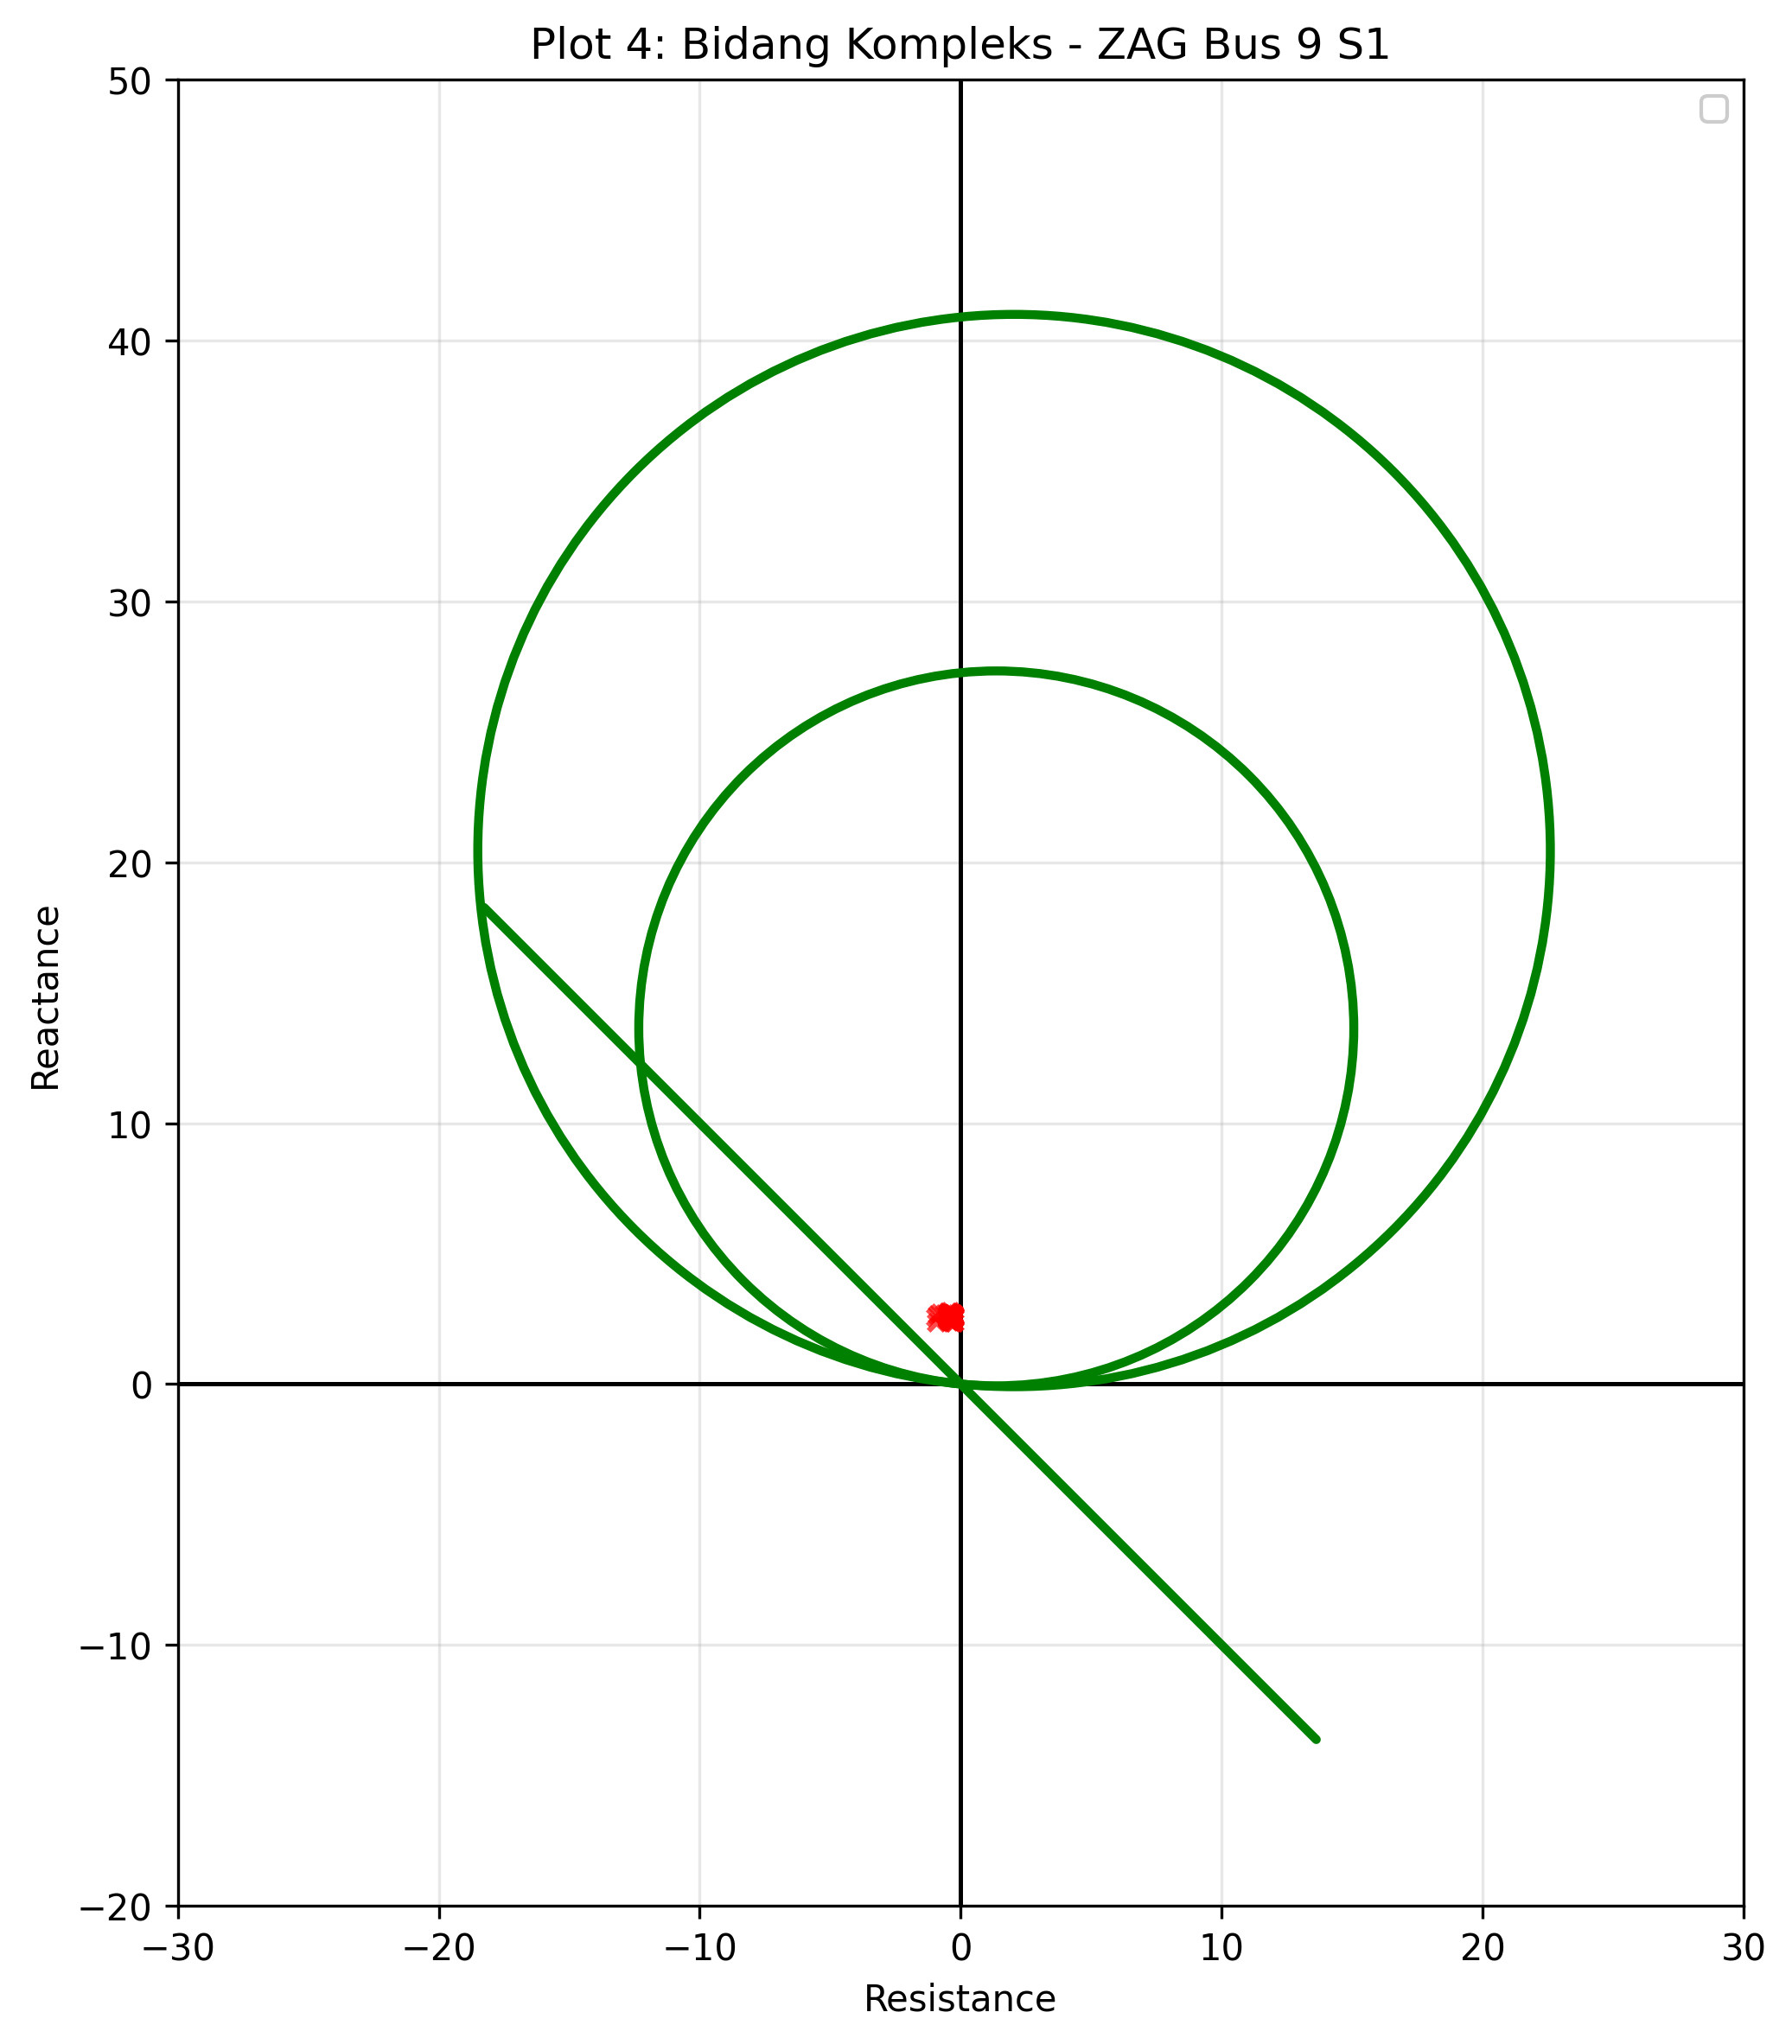
\includegraphics[width=0.8\textwidth]{contents/chapter-4/PRIZI_04_ZAG_Bus_9_S1.png}
%     \caption{Impedansi Tampak ZAG Bus 9 Skenario 1}
%     \label{fig:PRIZI_04_ZAG_Bus_9_S1}
% \end{figure}

\begin{figure}[H]
    \centering

    % Gambar sebelah kiri
    \begin{subfigure}[t]{0.48\textwidth}
        \centering
        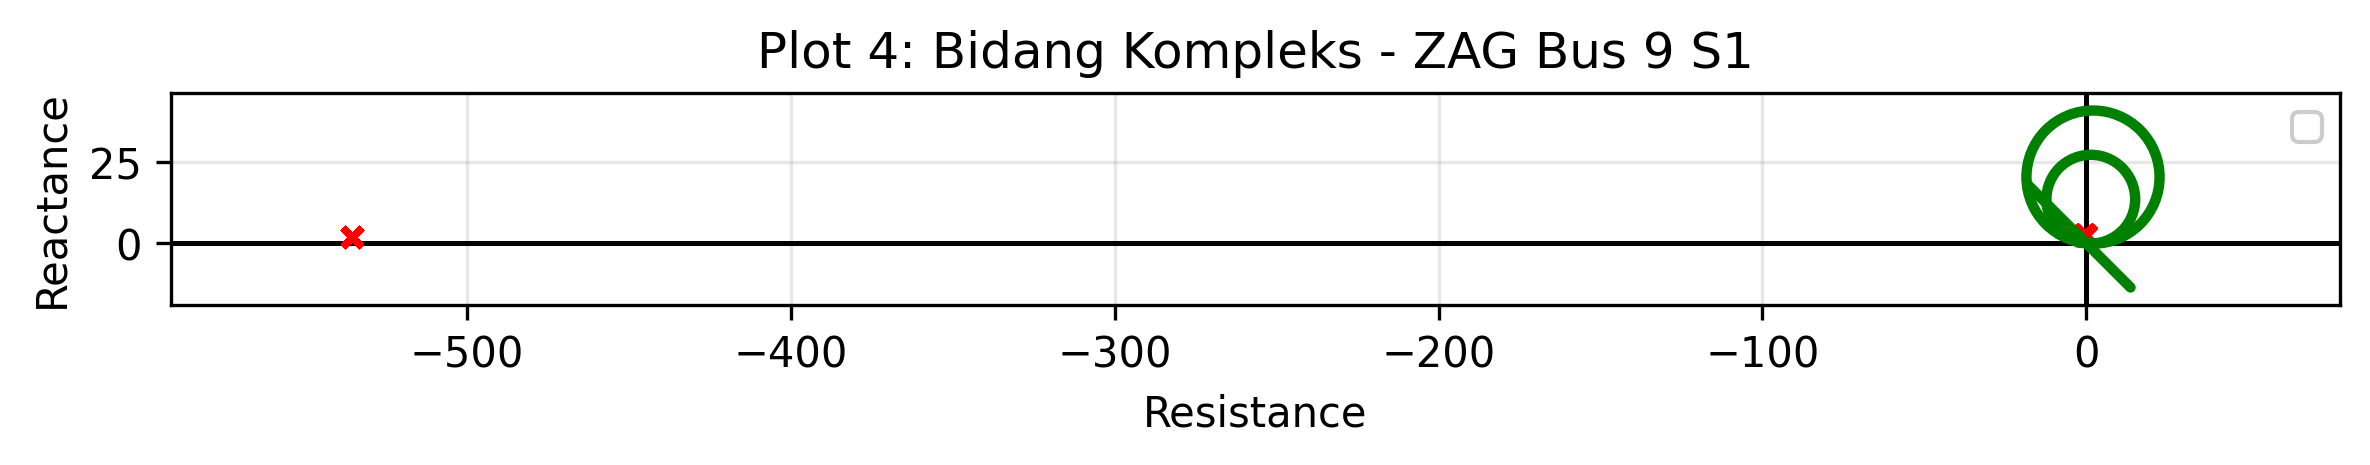
\includegraphics[width=\textwidth]{contents/chapter-4/PRIA_04_ZAG_Bus_9_S1.png}
        \caption{Seluruh Impedansi Tampak}
        \label{fig:PRIA_04_ZAG_Bus_9_S1}
    \end{subfigure}
    \hfill
    % Gambar sebelah kanan
    \begin{subfigure}[t]{0.48\textwidth}
        \centering
        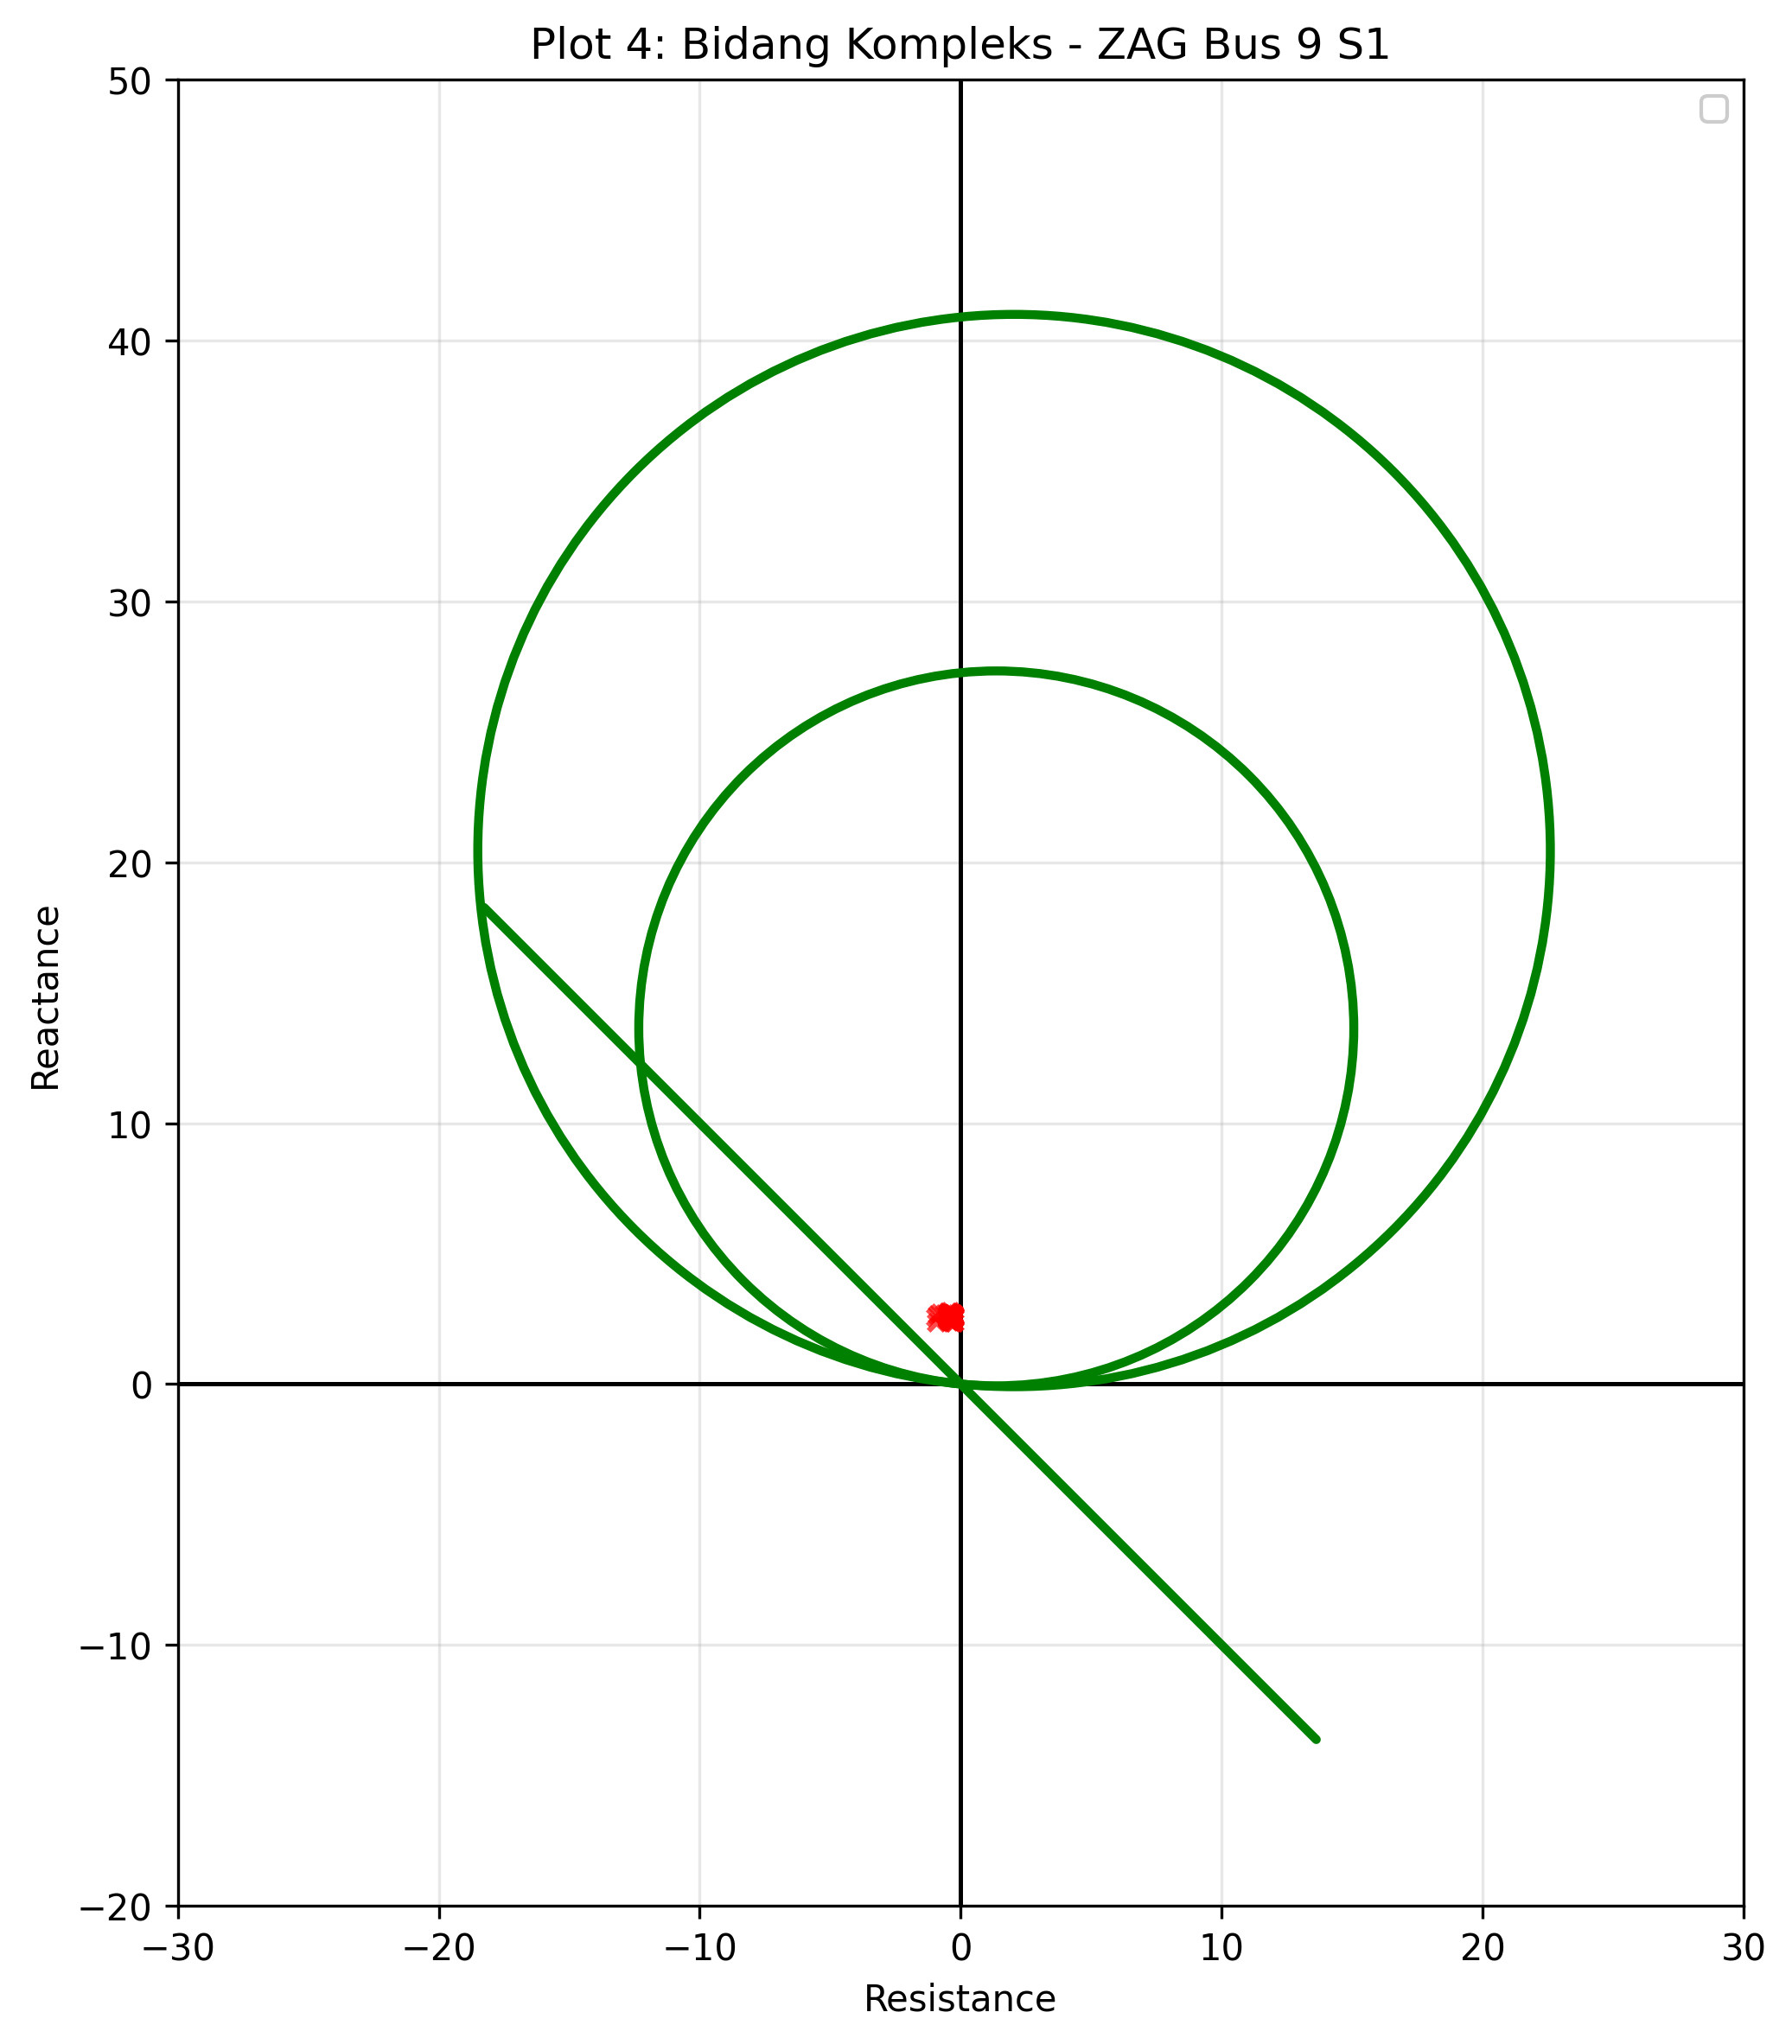
\includegraphics[width=\textwidth]{contents/chapter-4/PRIZI_04_ZAG_Bus_9_S1.png}
        \caption{Zoom In Pada Zona Proteksi}
        \label{fig:PRIZI_04_ZAG_Bus_9_S1}
    \end{subfigure}

    \caption{Impedansi Tampak ZAG Bus 9 Skenario 1}
    \label{fig:Impedansi_Tampak_ZAG_Bus_9_S1}
\end{figure}

Pada gambar \ref{fig:Impedansi_Tampak_ZAG_Bus_9_S1} terlihat untuk titik impedansi tampak pada fasa A dan ground yang di baca relay 21 dari sisi bus 9 memasuki zona 1 namun tidak terbaca sebagai gangguan karena elemen fasa directional tidak membaca bahwa gangguan terdapat di depan relay maka relay 21 bus 9 bekerja dengan baik sebagaimana mestinya dengan acuan pada \ref{subsec:tanpa_IBR_in_dlg} karena kontribusi dari sisi IBR tidak mendominasi karena TL78 tetap aktif mengakibatkan IBR tidak memengaruhi kinerja proteksi serta kontribusi tetap di dominasi oleh sistem tenaga konvensional.

%%%%%%%%%%%%%%%%%%%%%%%%%%%%%%%%%%%%%%%%%%%%%%%%%%%%%%%%%%%%%%%

% \begin{figure}[H]
%     \centering
%     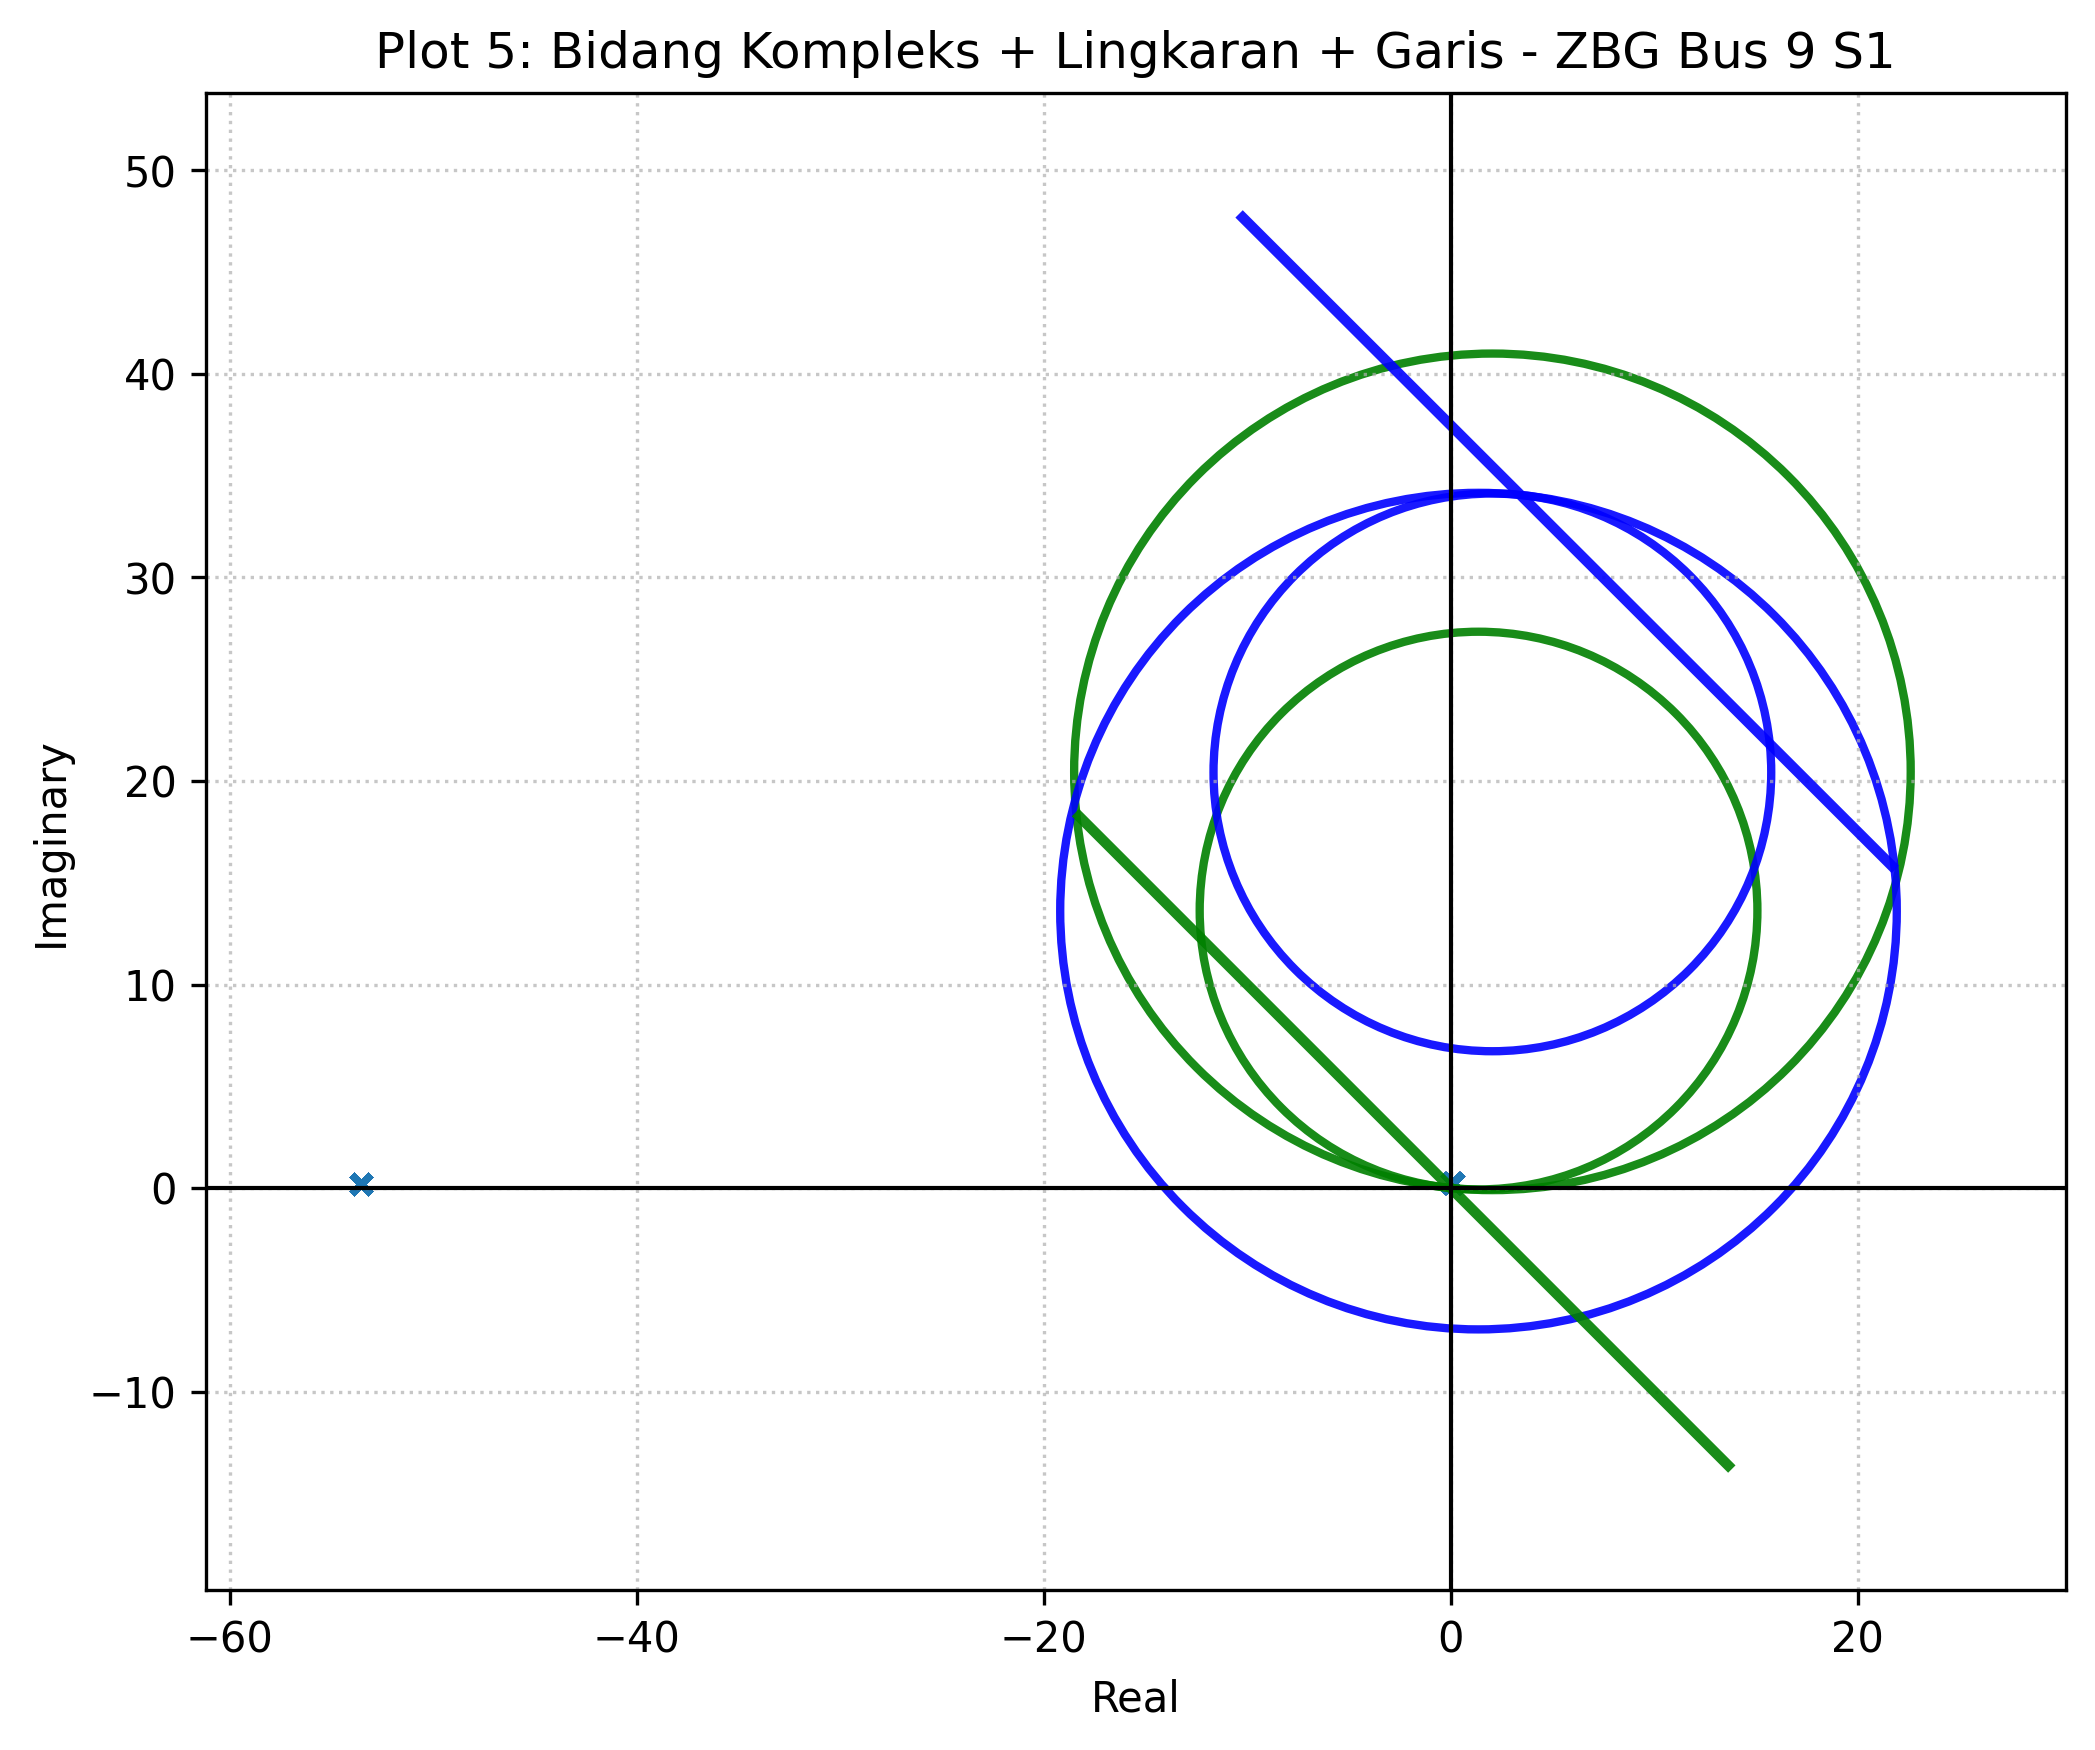
\includegraphics[width=0.8\textwidth]{contents/chapter-4/05_ZBG_Bus_9_S1_dengan_lingkaran_dan_garis.png}
%     \caption{Impedansi Tampak ZBG Bus 9 Skenario 1}
%     \label{fig:05_ZBG_Bus_9_S1_dengan_lingkaran_dan_garis}
% \end{figure}

% Pada gambar \ref{fig:05_ZBG_Bus_9_S1_dengan_lingkaran_dan_garis} terlihat untuk titik impedansi tampak pada fasa B dan ground terlihat cukup stabil dan relay 21 dari sisi bus 9 bekerja dengan normal sebagaimana mestinya dengan acuan pada \ref{subsec:tanpa_IBR_in_dlg} karena kontribusi dari sisi IBR tidak mendominasi karena TL78 tetap aktif mengakibatkan IBR tidak memengaruhi kinerja proteksi serta kontribusi tetap di dominasi oleh sistem tenaga konvensional.

%%%%%%%%%%%%%%%%%%%%%%%%%%%%%%%%%SISI PRIMER%%%%%%%%%%%%%%%%%%%%%%%%%%%%%%%%%%

% \begin{figure}[H]
%     \centering
%     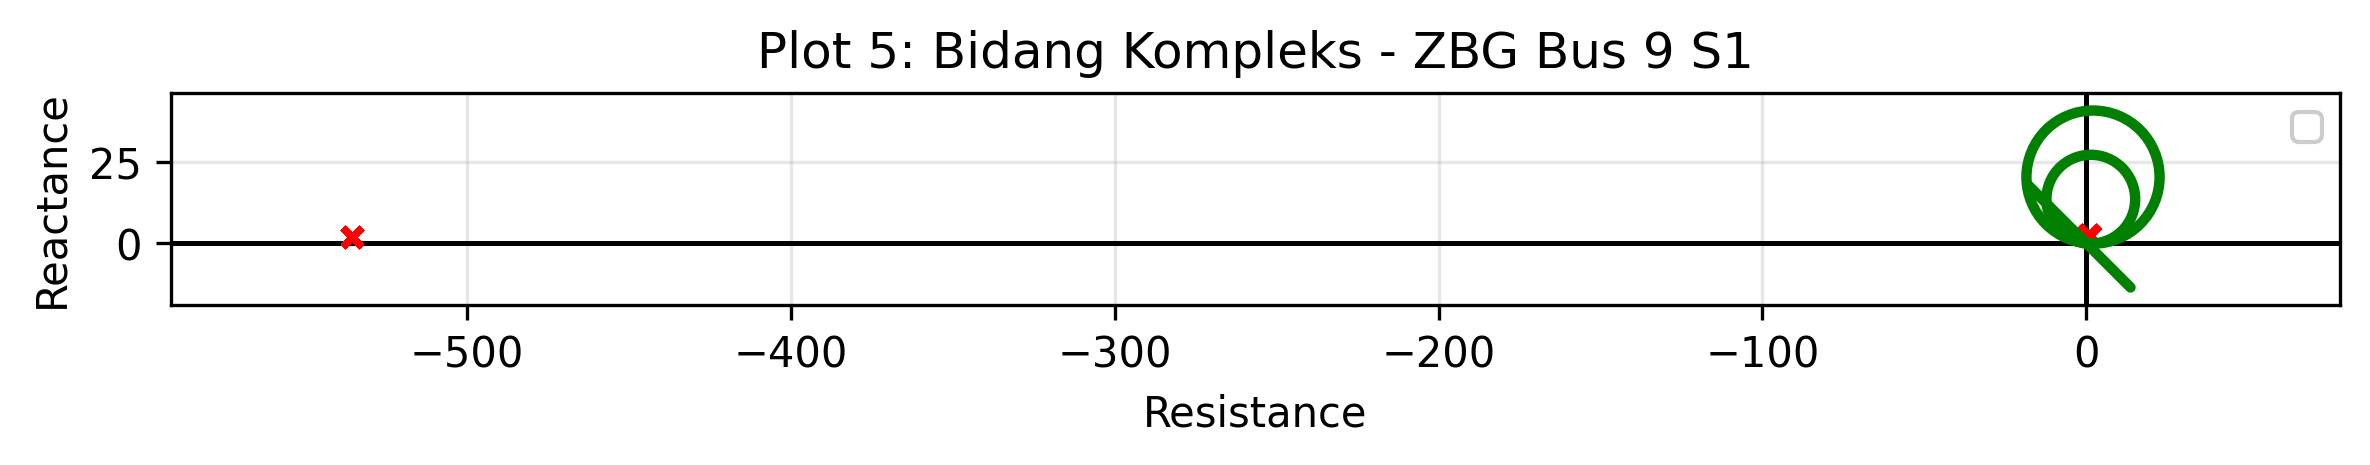
\includegraphics[width=0.8\textwidth]{contents/chapter-4/PRIA_05_ZBG_Bus_9_S1.png}
%     \caption{Impedansi Tampak ZBG Bus 9 Skenario 1}
%     \label{fig:PRIA_05_ZBG_Bus_9_S1}
% \end{figure}

% \begin{figure}[H]
%     \centering
%     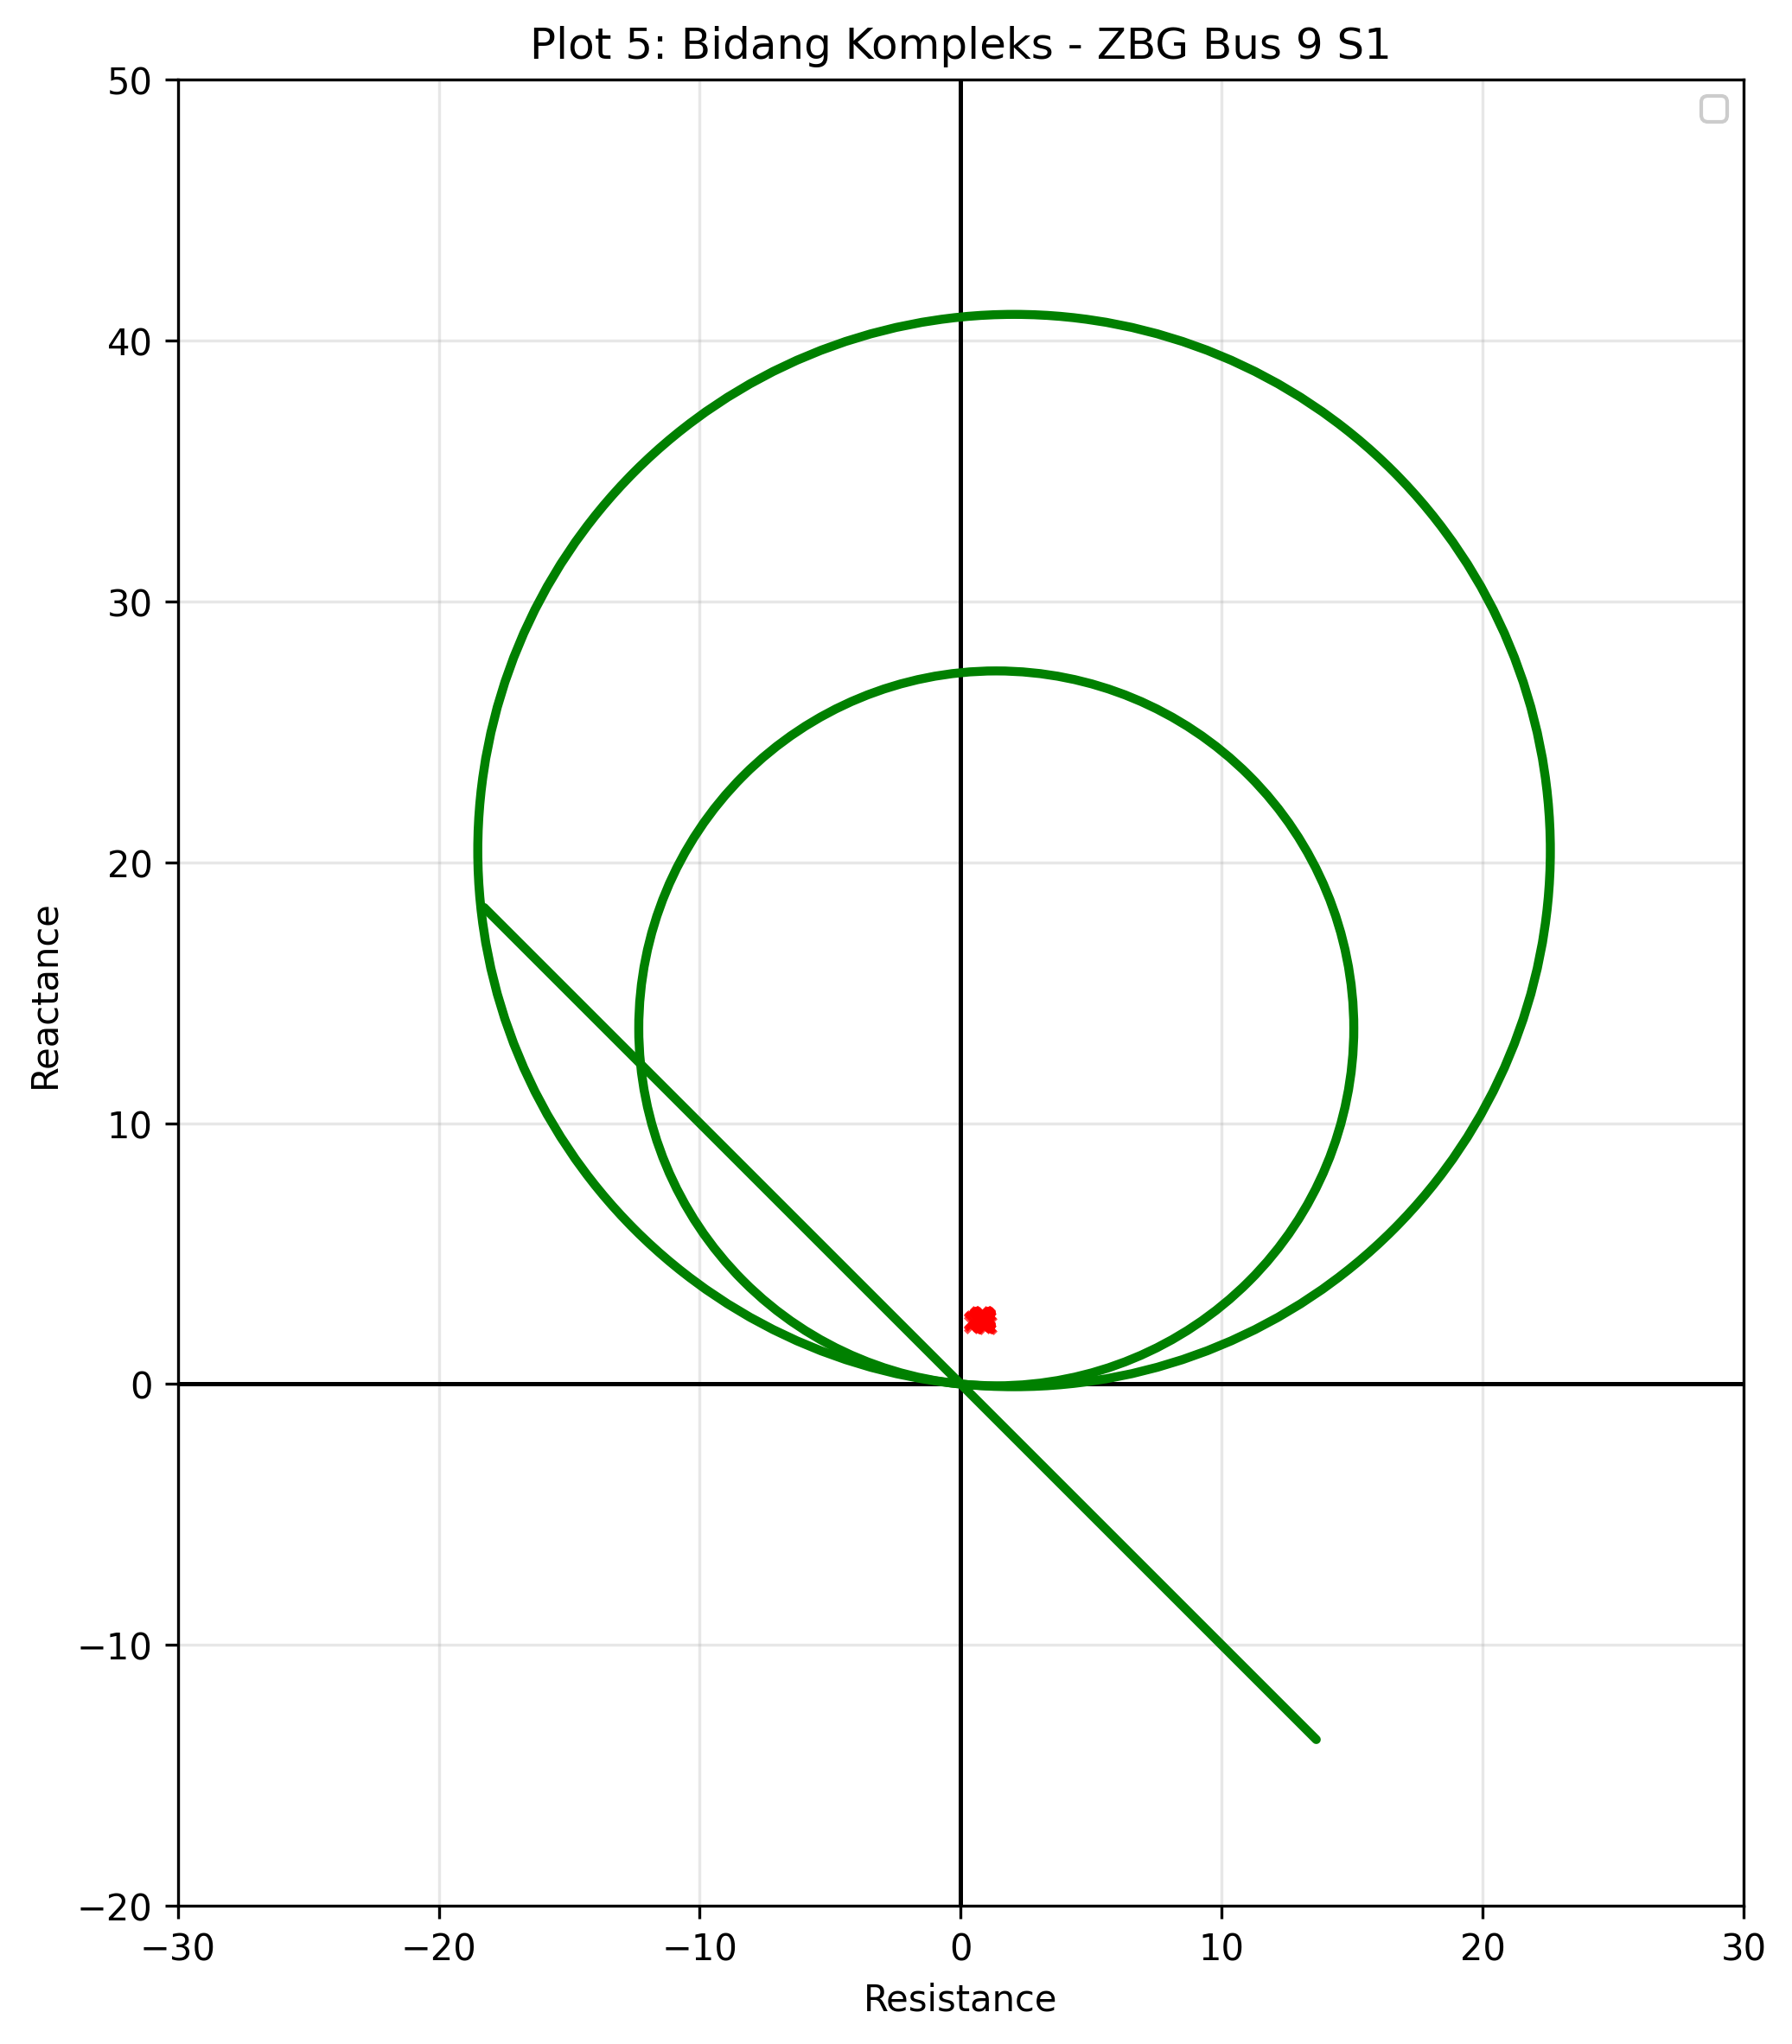
\includegraphics[width=0.8\textwidth]{contents/chapter-4/PRIZI_05_ZBG_Bus_9_S1.png}
%     \caption{Impedansi Tampak ZBG Bus 9 Skenario 1}
%     \label{fig:PRIZI_05_ZBG_Bus_9_S1}
% \end{figure}

\begin{figure}[H]
    \centering

    % Gambar sebelah kiri
    \begin{subfigure}[t]{0.48\textwidth}
        \centering
        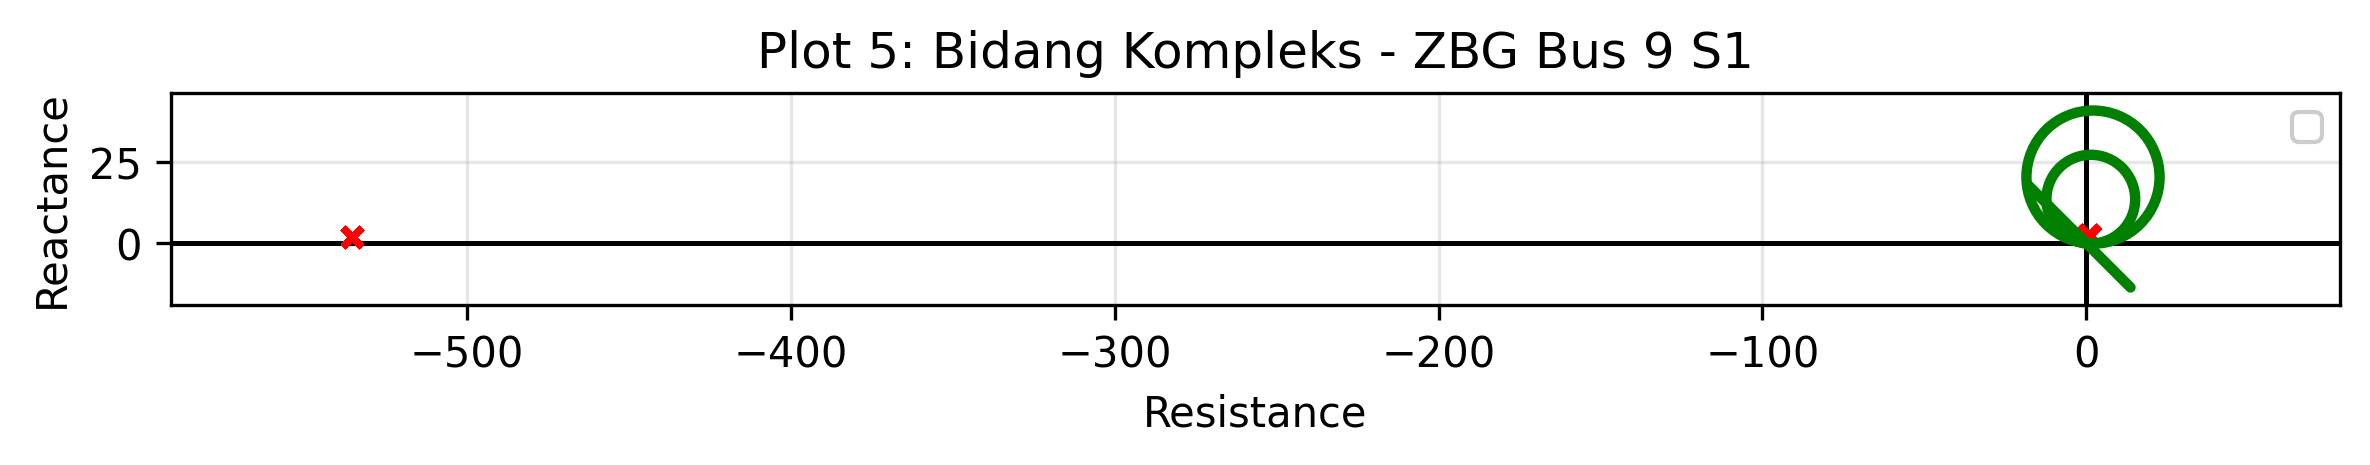
\includegraphics[width=\textwidth]{contents/chapter-4/PRIA_05_ZBG_Bus_9_S1.png}
        \caption{Seluruh Impedansi Tampak}
        \label{fig:PRIA_05_ZBG_Bus_9_S1}
    \end{subfigure}
    \hfill
    % Gambar sebelah kanan
    \begin{subfigure}[t]{0.48\textwidth}
        \centering
        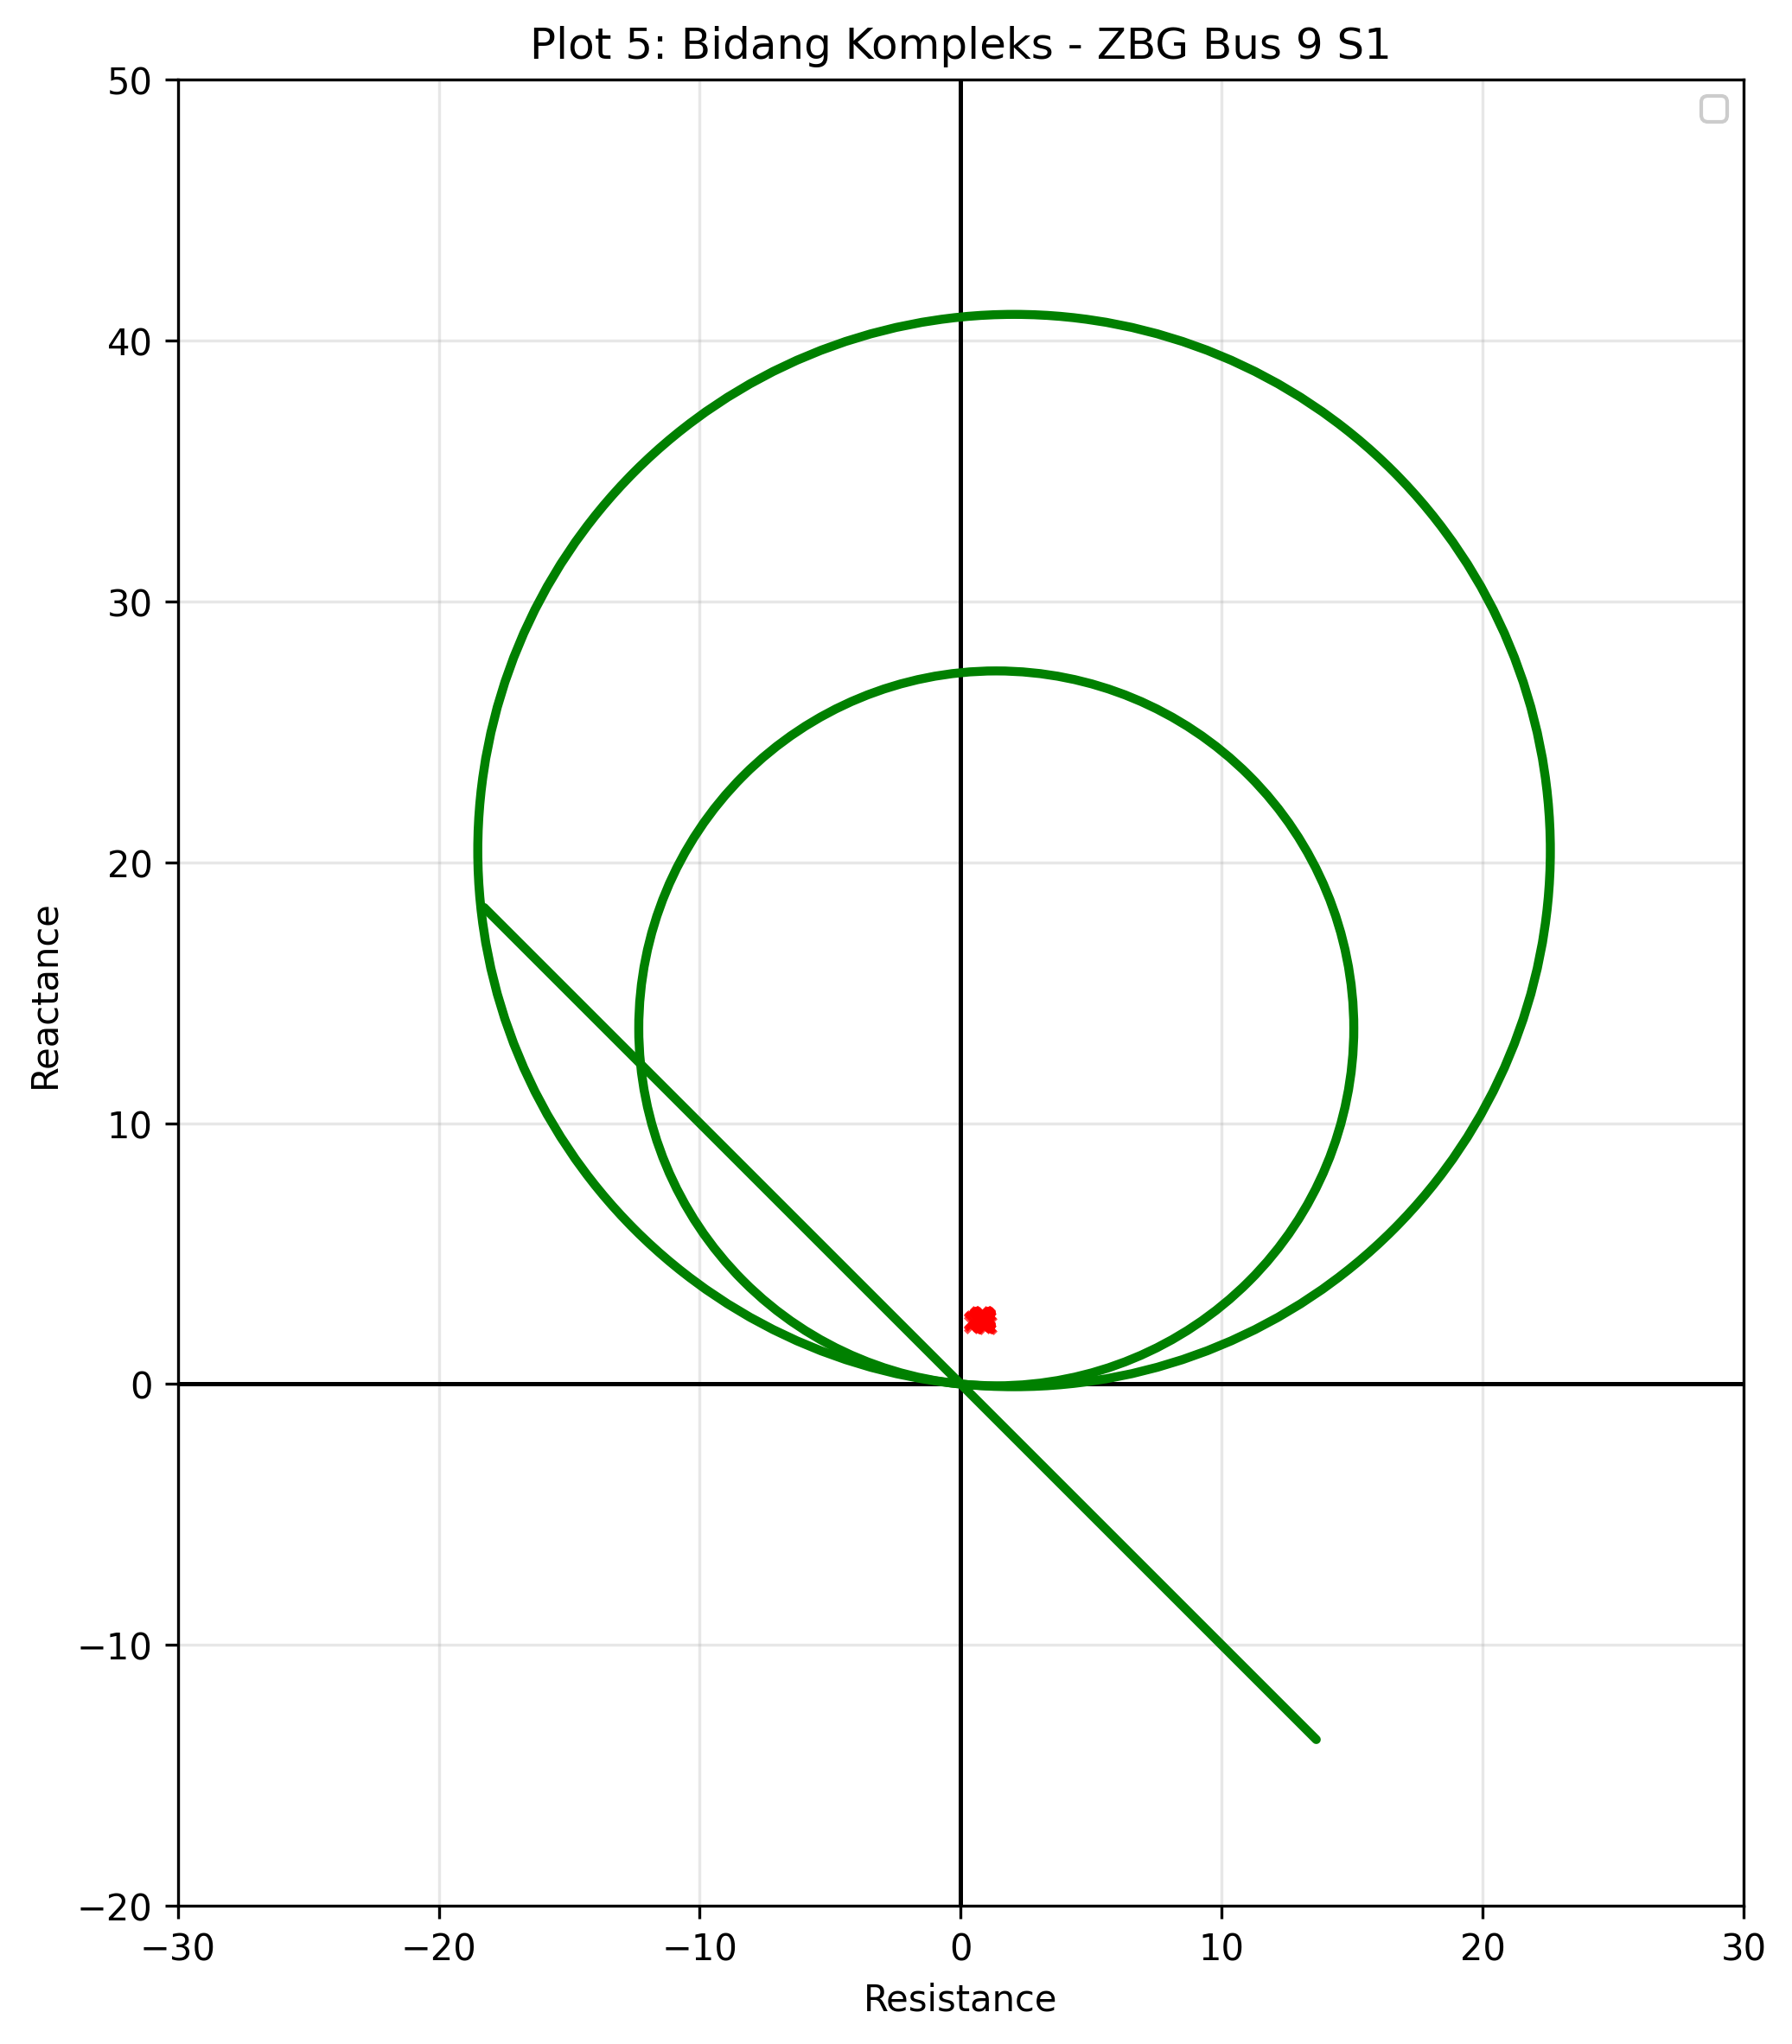
\includegraphics[width=\textwidth]{contents/chapter-4/PRIZI_05_ZBG_Bus_9_S1.png}
        \caption{Zoom In Pada Zona Proteksi}
        \label{fig:PRIZI_05_ZBG_Bus_9_S1}
    \end{subfigure}

    \caption{Impedansi Tampak ZBG Bus 9 Skenario 1}
    \label{fig:Impedansi_Tampak_ZBG_Bus_9_S1}
\end{figure}

Pada gambar \ref{fig:Impedansi_Tampak_ZBG_Bus_9_S1} terlihat untuk titik impedansi tampak pada fasa B dan ground yang di baca relay 21 dari sisi bus 9 memasuki zona 1 namun tidak terbaca sebagai gangguan karena elemen fasa directional tidak membaca bahwa gangguan terdapat di depan relay maka relay 21 bus 9 bekerja dengan baik sebagaimana mestinya dengan acuan pada \ref{subsec:tanpa_IBR_in_dlg} karena kontribusi dari sisi IBR tidak mendominasi karena TL78 tetap aktif mengakibatkan IBR tidak memengaruhi kinerja proteksi serta kontribusi tetap di dominasi oleh sistem tenaga konvensional.

%%%%%%%%%%%%%%%%%%%%%%%%%%%%%%%%%%%%%%%%%%%%%%%%%%%%%%%%%%%%%%%

% \begin{figure}[H]
%     \centering
%     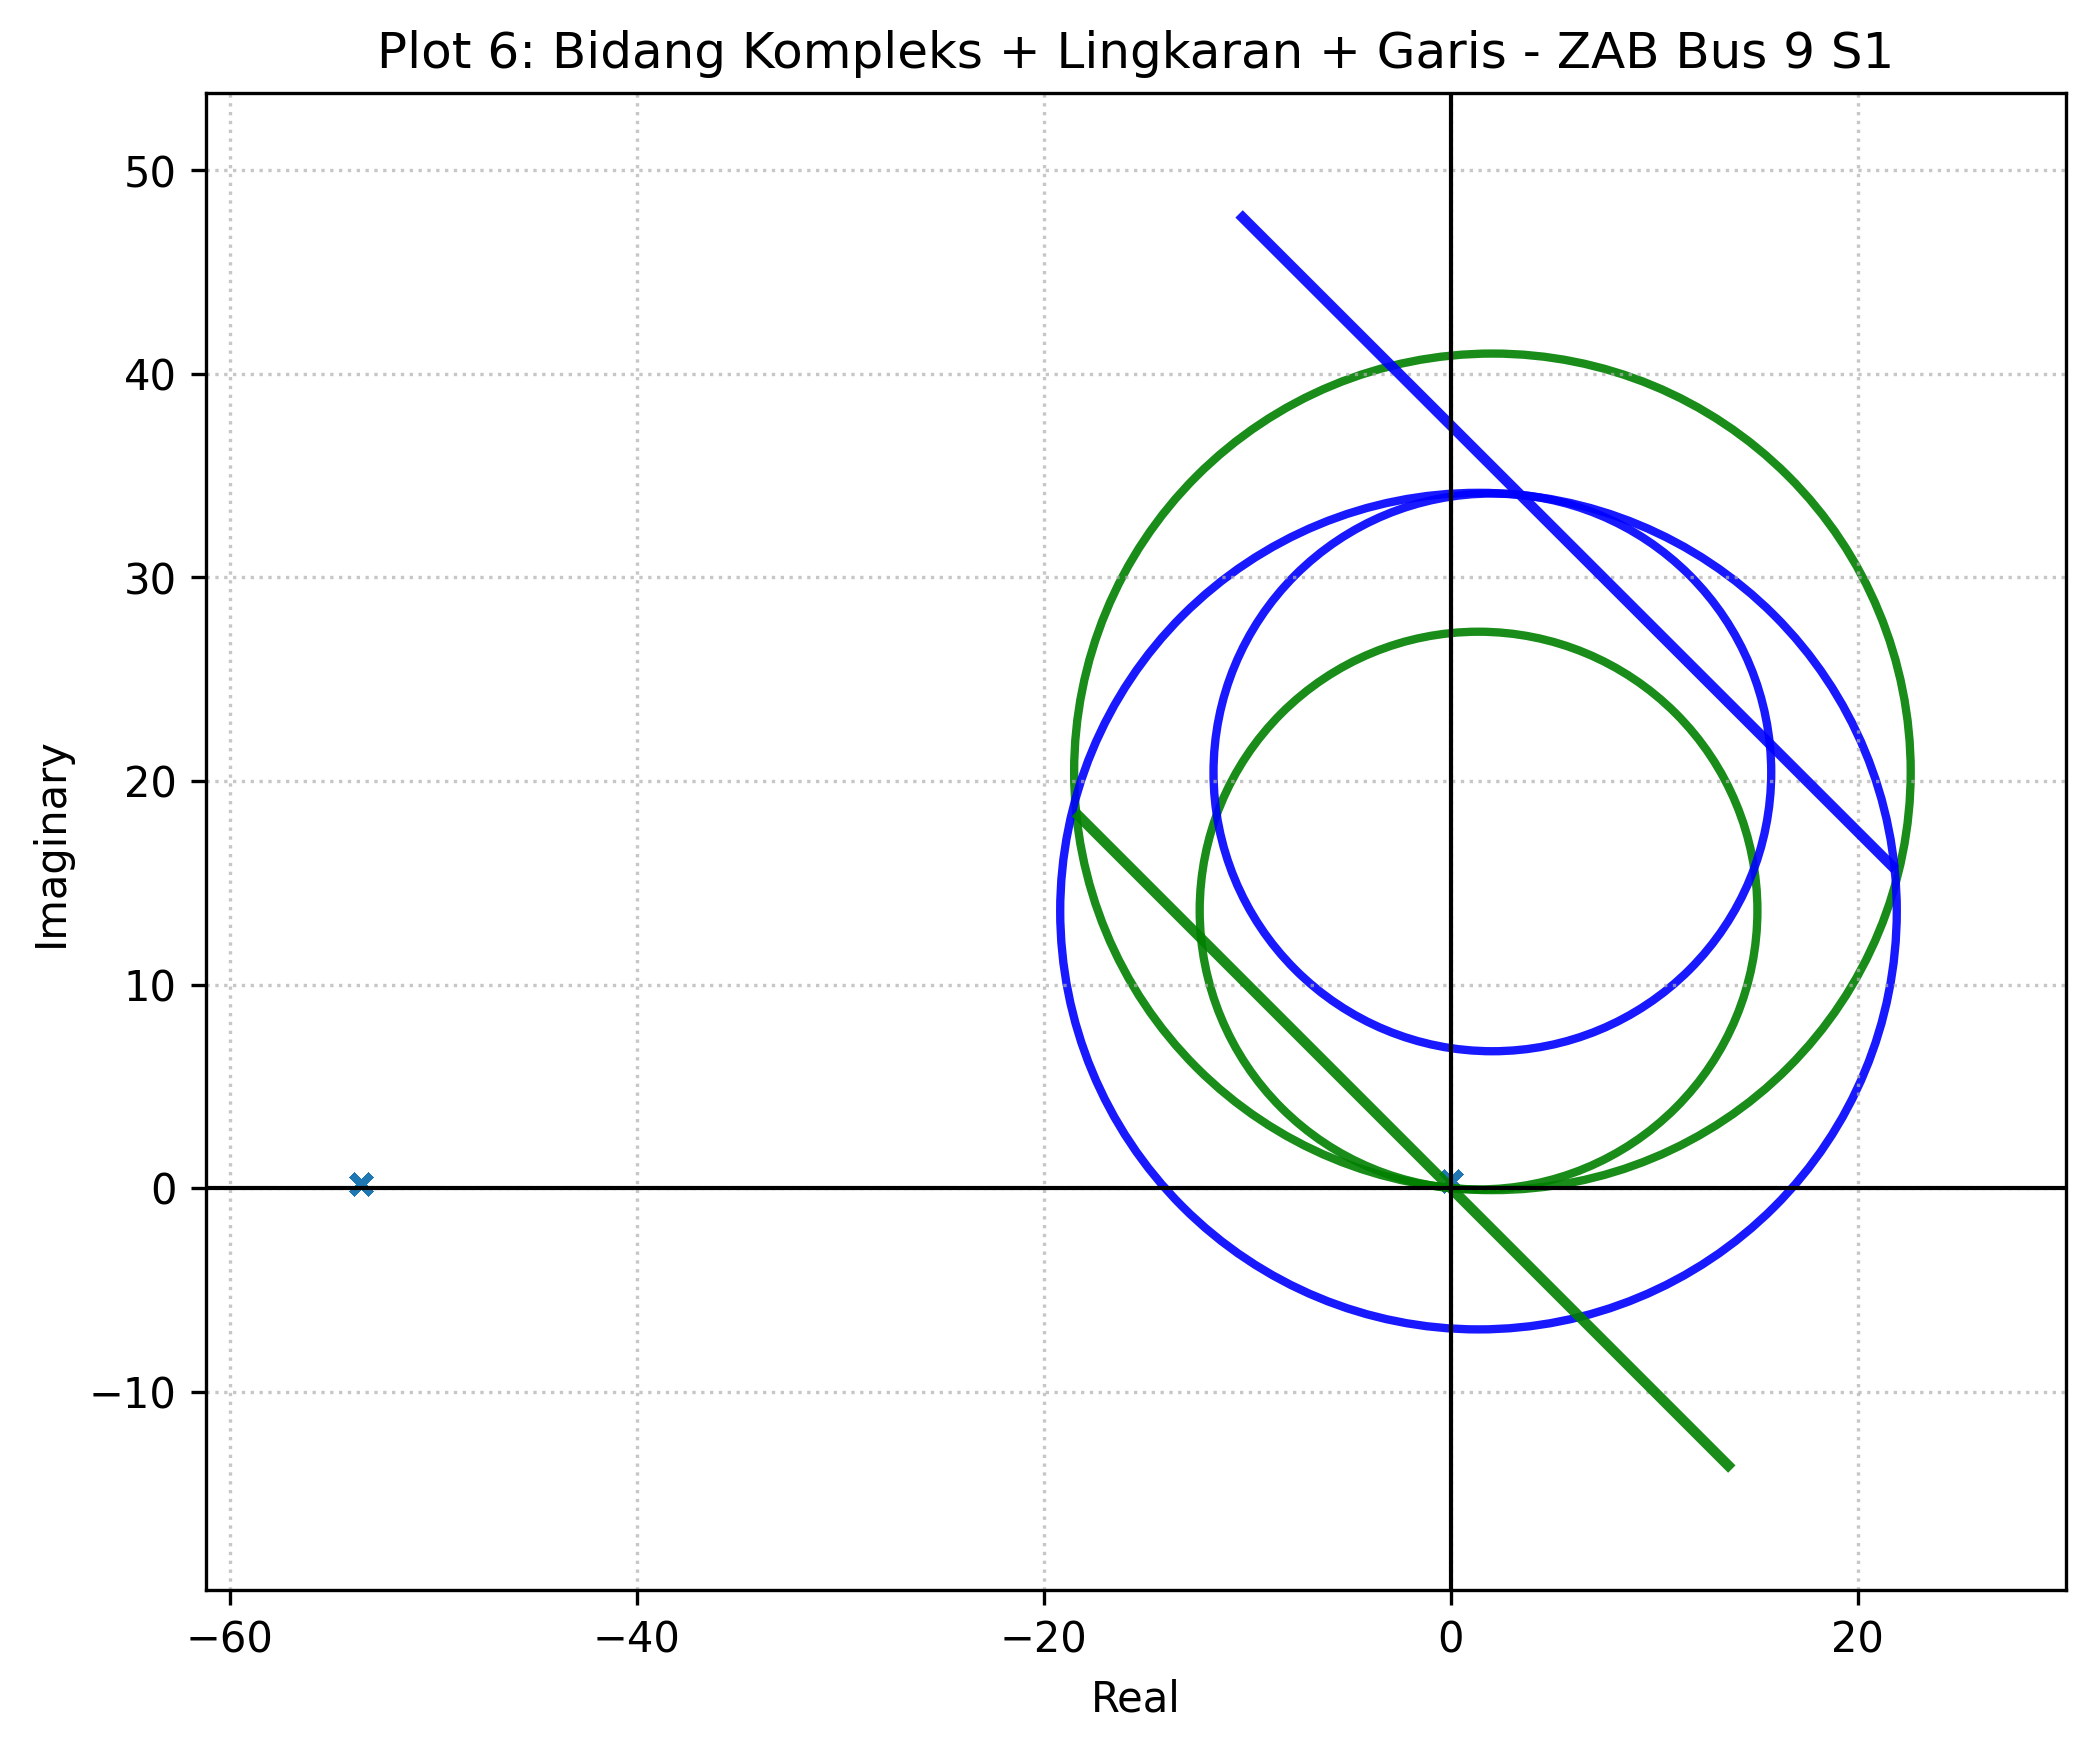
\includegraphics[width=0.8\textwidth]{contents/chapter-4/06_ZAB_Bus_9_S1_dengan_lingkaran_dan_garis.png}
%     \caption{Impedansi Tampak ZAB Bus 9 Skenario 1}
%     \label{fig:06_ZAB_Bus_9_S1_dengan_lingkaran_dan_garis}
% \end{figure}

% Pada gambar \ref{fig:06_ZAB_Bus_9_S1_dengan_lingkaran_dan_garis} terlihat untuk titik impedansi tampak pada fasa A dan fasa B terlihat cukup stabil dan relay 21 dari sisi bus 9 bekerja dengan normal sebagaimana mestinya dengan acuan pada \ref{subsec:tanpa_IBR_in_dlg} karena kontribusi dari sisi IBR tidak mendominasi karena TL78 tetap aktif mengakibatkan IBR tidak memengaruhi kinerja proteksi serta kontribusi tetap di dominasi oleh sistem tenaga konvensional.

%%%%%%%%%%%%%%%%%%%%%%%%%%%%%%%%%SISI PRIMER%%%%%%%%%%%%%%%%%%%%%%%%%%%%%%%%%%

% \begin{figure}[H]
%     \centering
%     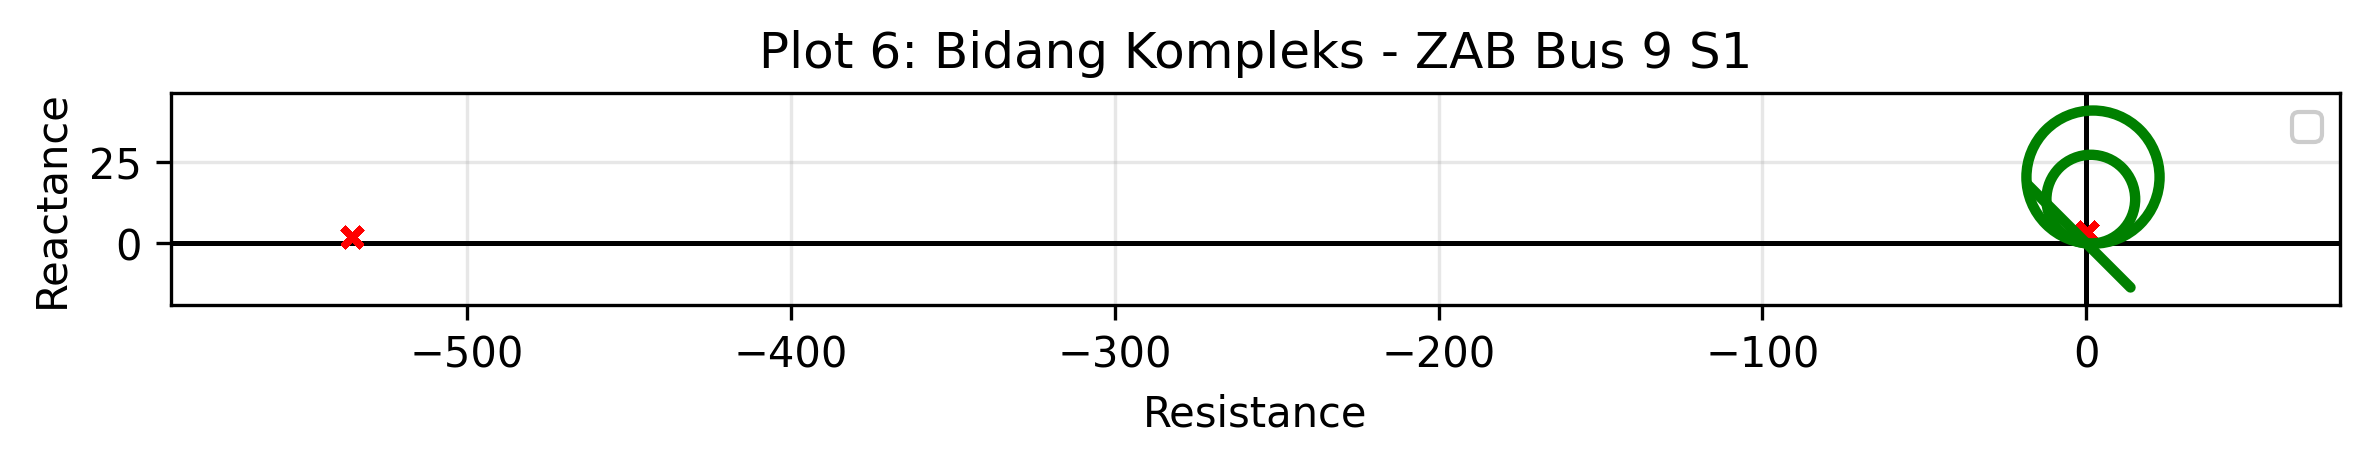
\includegraphics[width=0.8\textwidth]{contents/chapter-4/PRIA_06_ZAB_Bus_9_S1.png}
%     \caption{Impedansi Tampak ZAB Bus 9 Skenario 1}
%     \label{fig:PRIA_06_ZAB_Bus_9_S1}
% \end{figure}

% \begin{figure}[H]
%     \centering
%     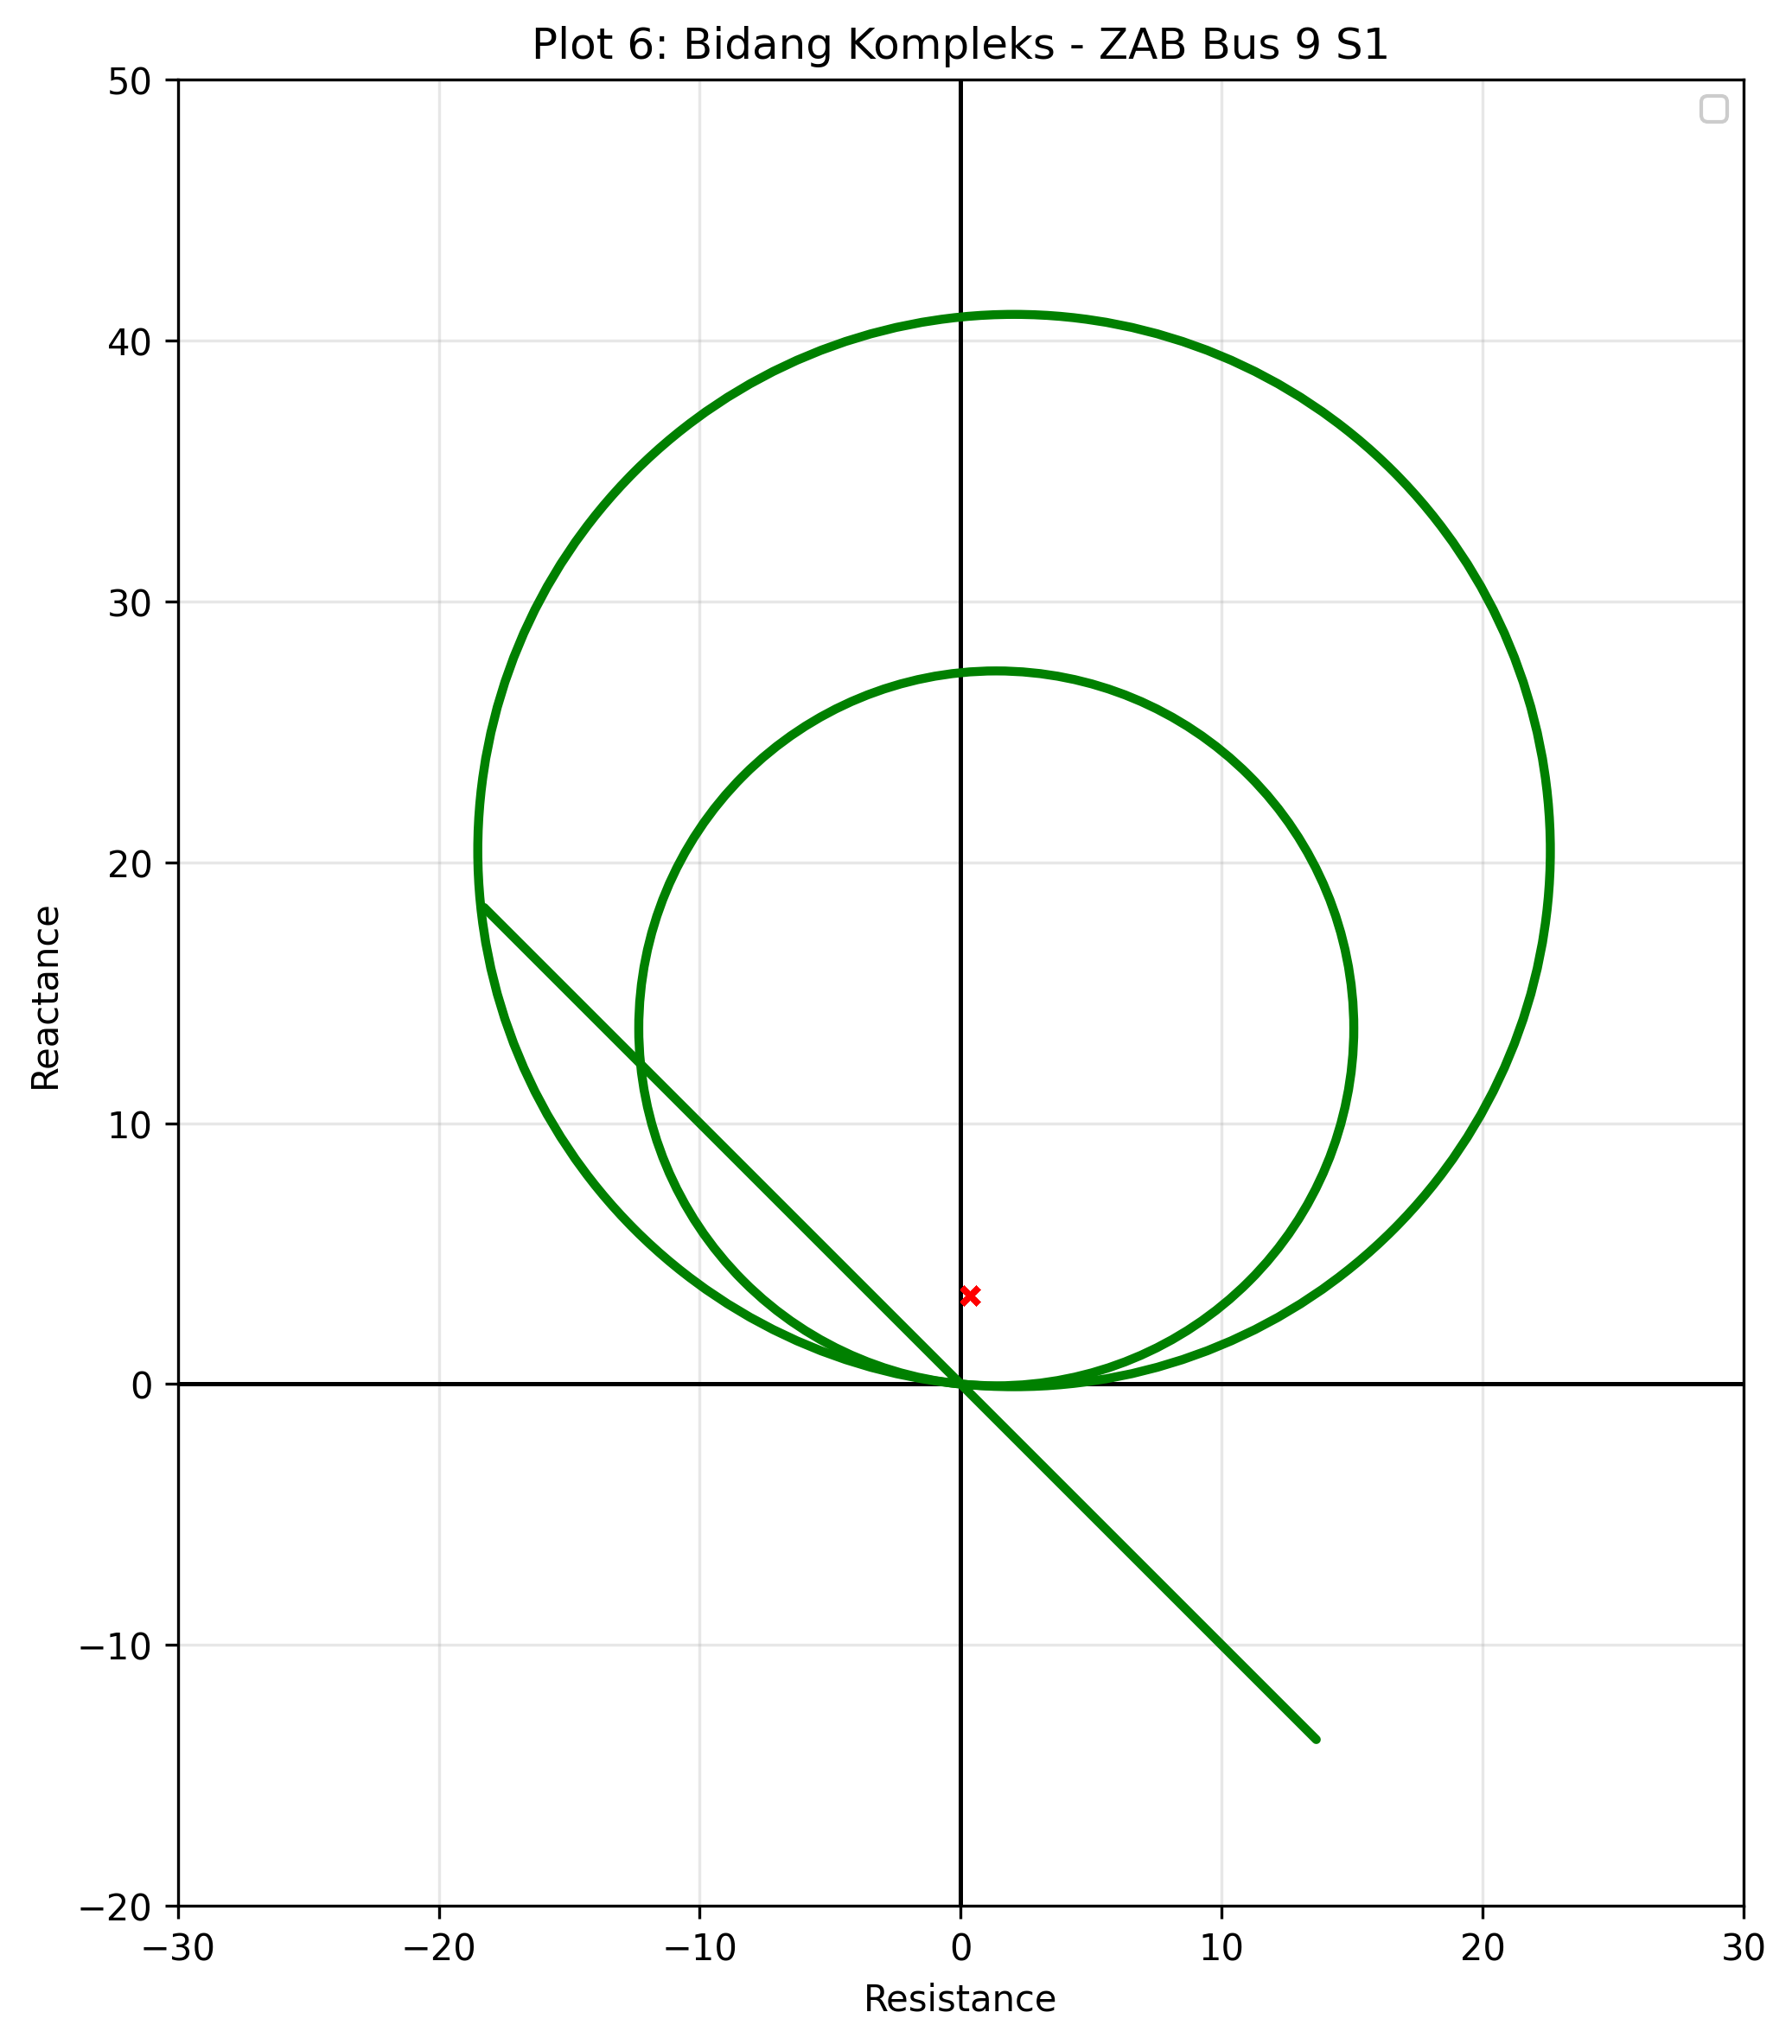
\includegraphics[width=0.8\textwidth]{contents/chapter-4/PRIZI_06_ZAB_Bus_9_S1.png}
%     \caption{Impedansi Tampak ZAB Bus 9 Skenario 1}
%     \label{fig:PRIZI_06_ZAB_Bus_9_S1}
% \end{figure}

\begin{figure}[H]
    \centering

    % Gambar sebelah kiri
    \begin{subfigure}[t]{0.48\textwidth}
        \centering
        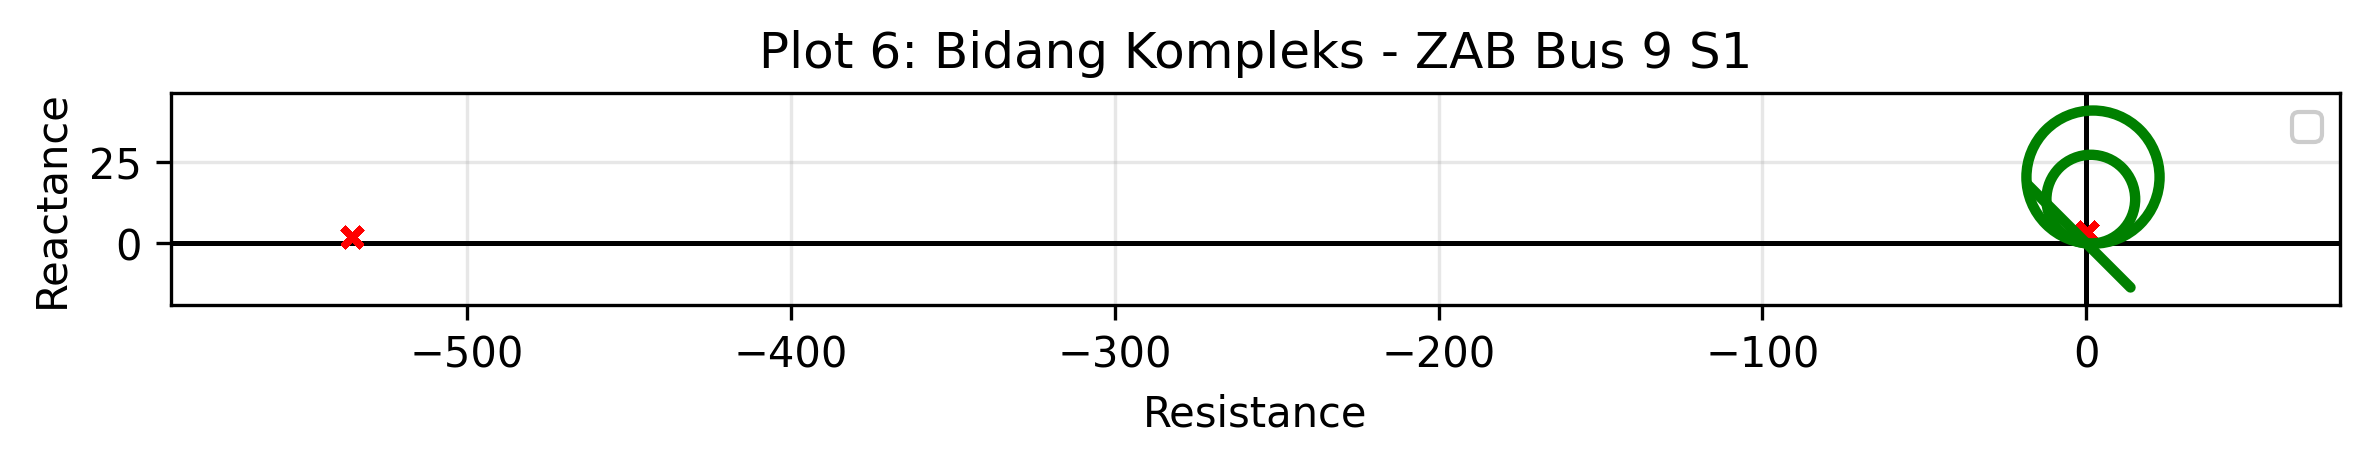
\includegraphics[width=\textwidth]{contents/chapter-4/PRIA_06_ZAB_Bus_9_S1.png}
        \caption{Seluruh Impedansi Tampak}
        \label{fig:PRIA_06_ZAB_Bus_9_S1}
    \end{subfigure}
    \hfill
    % Gambar sebelah kanan
    \begin{subfigure}[t]{0.48\textwidth}
        \centering
        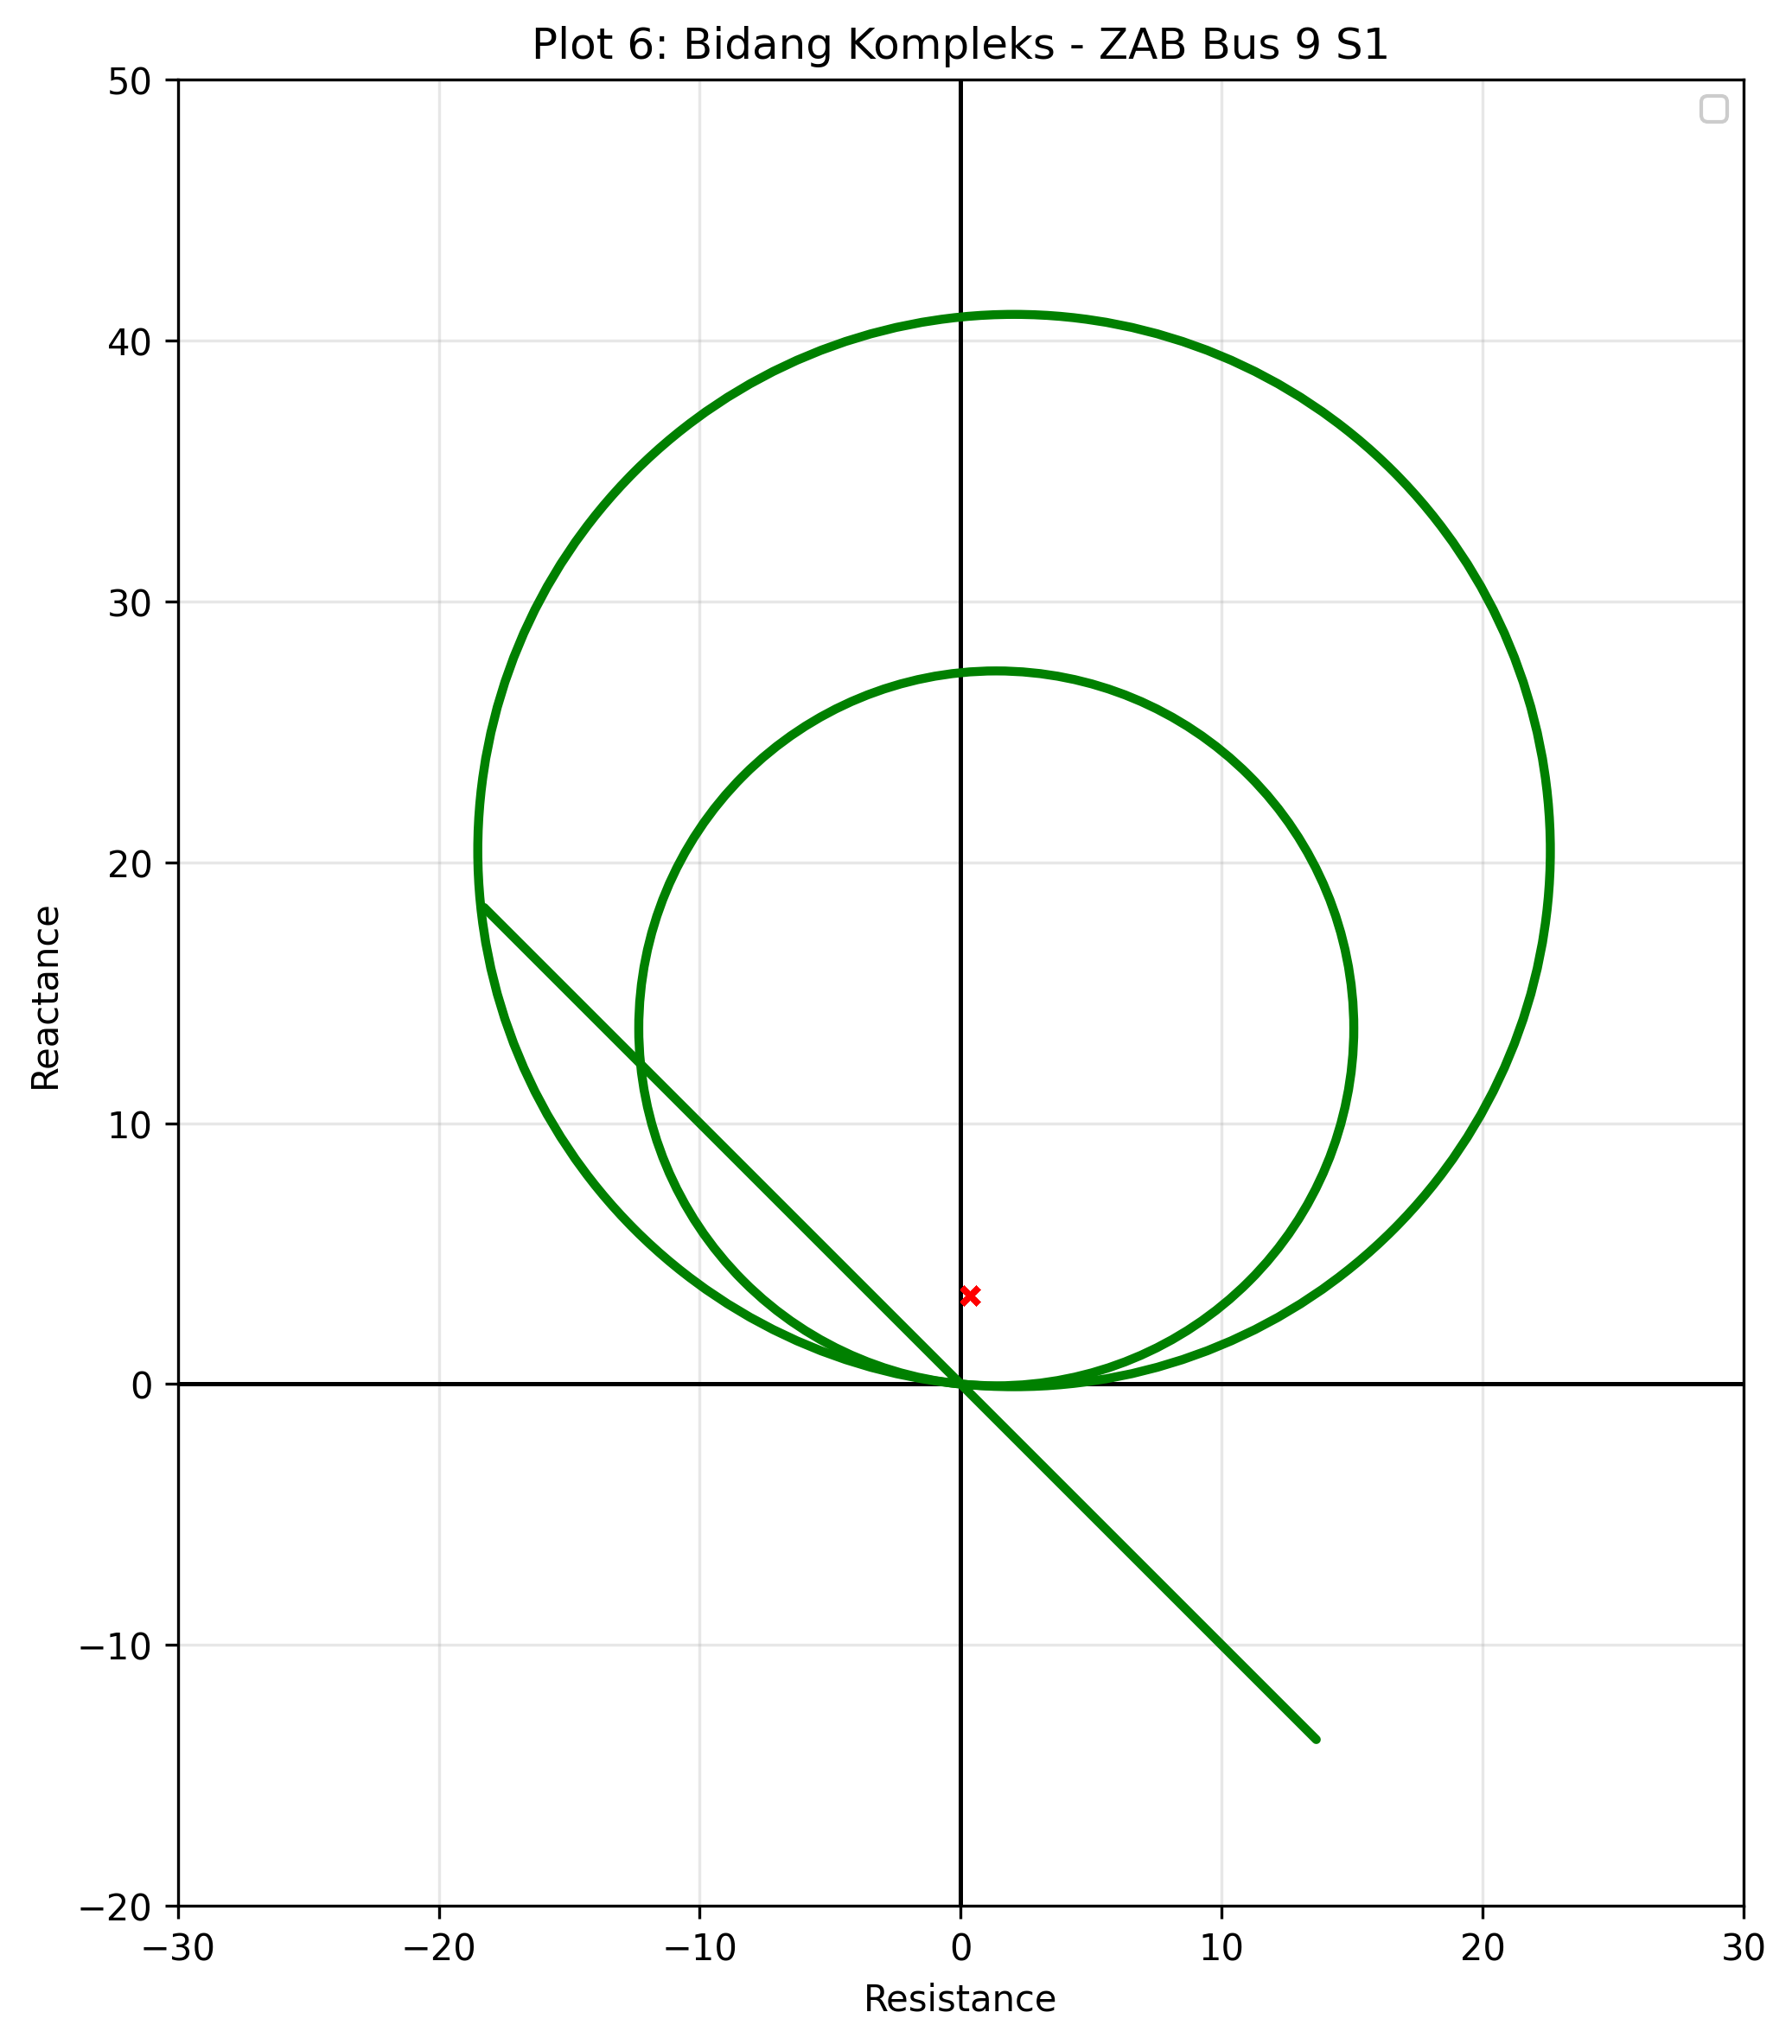
\includegraphics[width=\textwidth]{contents/chapter-4/PRIZI_06_ZAB_Bus_9_S1.png}
        \caption{Zoom In Pada Zona Proteksi}
        \label{fig:PRIZI_06_ZAB_Bus_9_S1}
    \end{subfigure}

    \caption{Impedansi Tampak ZAB Bus 9 Skenario 1}
    \label{fig:Impedansi_Tampak_ZAB_Bus_9_S1}
\end{figure}

Pada gambar \ref{fig:Impedansi_Tampak_ZAB_Bus_9_S1} terlihat untuk titik impedansi tampak pada fasa A dan fasa B yang di baca relay 21 dari sisi bus 9 memasuki zona 1 namun tidak terbaca sebagai gangguan karena elemen fasa directional tidak membaca bahwa gangguan terdapat di depan relay maka relay 21 bus 9 bekerja dengan baik sebagaimana mestinya dengan acuan pada \ref{subsec:tanpa_IBR_in_dlg} karena kontribusi dari sisi IBR tidak mendominasi karena TL78 tetap aktif mengakibatkan IBR tidak memengaruhi kinerja proteksi serta kontribusi tetap di dominasi oleh sistem tenaga konvensional.

%%%%%%%%%%%%%%%%%%%%%%%%%%%%%%%%%%%%%%%%%%%%%%%%%%%%%%%%%%%%%%%



% Pada gambar \ref{fig:01_ZAG_Bus_8_S1_dengan_lingkaran_dan_garis} hingga \ref{fig:06_ZAB_Bus_9_S1_dengan_lingkaran_dan_garis} terlihat untuk titik impedansi tampak ZAG, ZBG, dan ZAB terlihat cukup stabil dan relay 21 dari sisi bus 8 maupun bus 9 bekerja dengan normal sebagaimana mestinya dengan acuan pada \ref{subsec:tanpa_IBR_in_dlg} karena kontribusi dari sisi IBR tidak mendominasi karena TL78 tetap aktif mengakibatkan IBR tidak memengaruhi kinerja proteksi serta kontribusi tetap di dominasi oleh sistem tenaga konvensional.

\subsection{Skenario 3 : Wind Turbine Type 3 External DLG Fault}

Berbeda dengan skenario sebelumnya, gangguan pada skenario ini berada di luar saluran TL89 sehingga relay 21 seharusnya tidak membaca gangguan sebagai gangguan internal pada saluran yang diproteksi. Kondisi ini penting untuk mengevaluasi selektivitas relay ketika sistem telah terintegrasi \textit{wind turbine type 3} dan konfigurasi jaringan berubah sesuai skenario pengujian.

Hasil dekomposisi komponen urutan arus pada Gambar \ref{fig:decomposition_sequence_current_s3} menjadi dasar untuk melihat perubahan besaran arus yang diterima oleh saluran TL89 pada gangguan eksternal DLG. Oleh karena itu, pembahasan pada subbab ini diarahkan untuk menelusuri apakah perubahan komponen arus tersebut memengaruhi syarat \textit{starting}, posisi impedansi tampak, dan keputusan trip relay 21 pada sisi Bus 8 dan Bus 9.

% \begin{figure}[H]
%     \centering
%     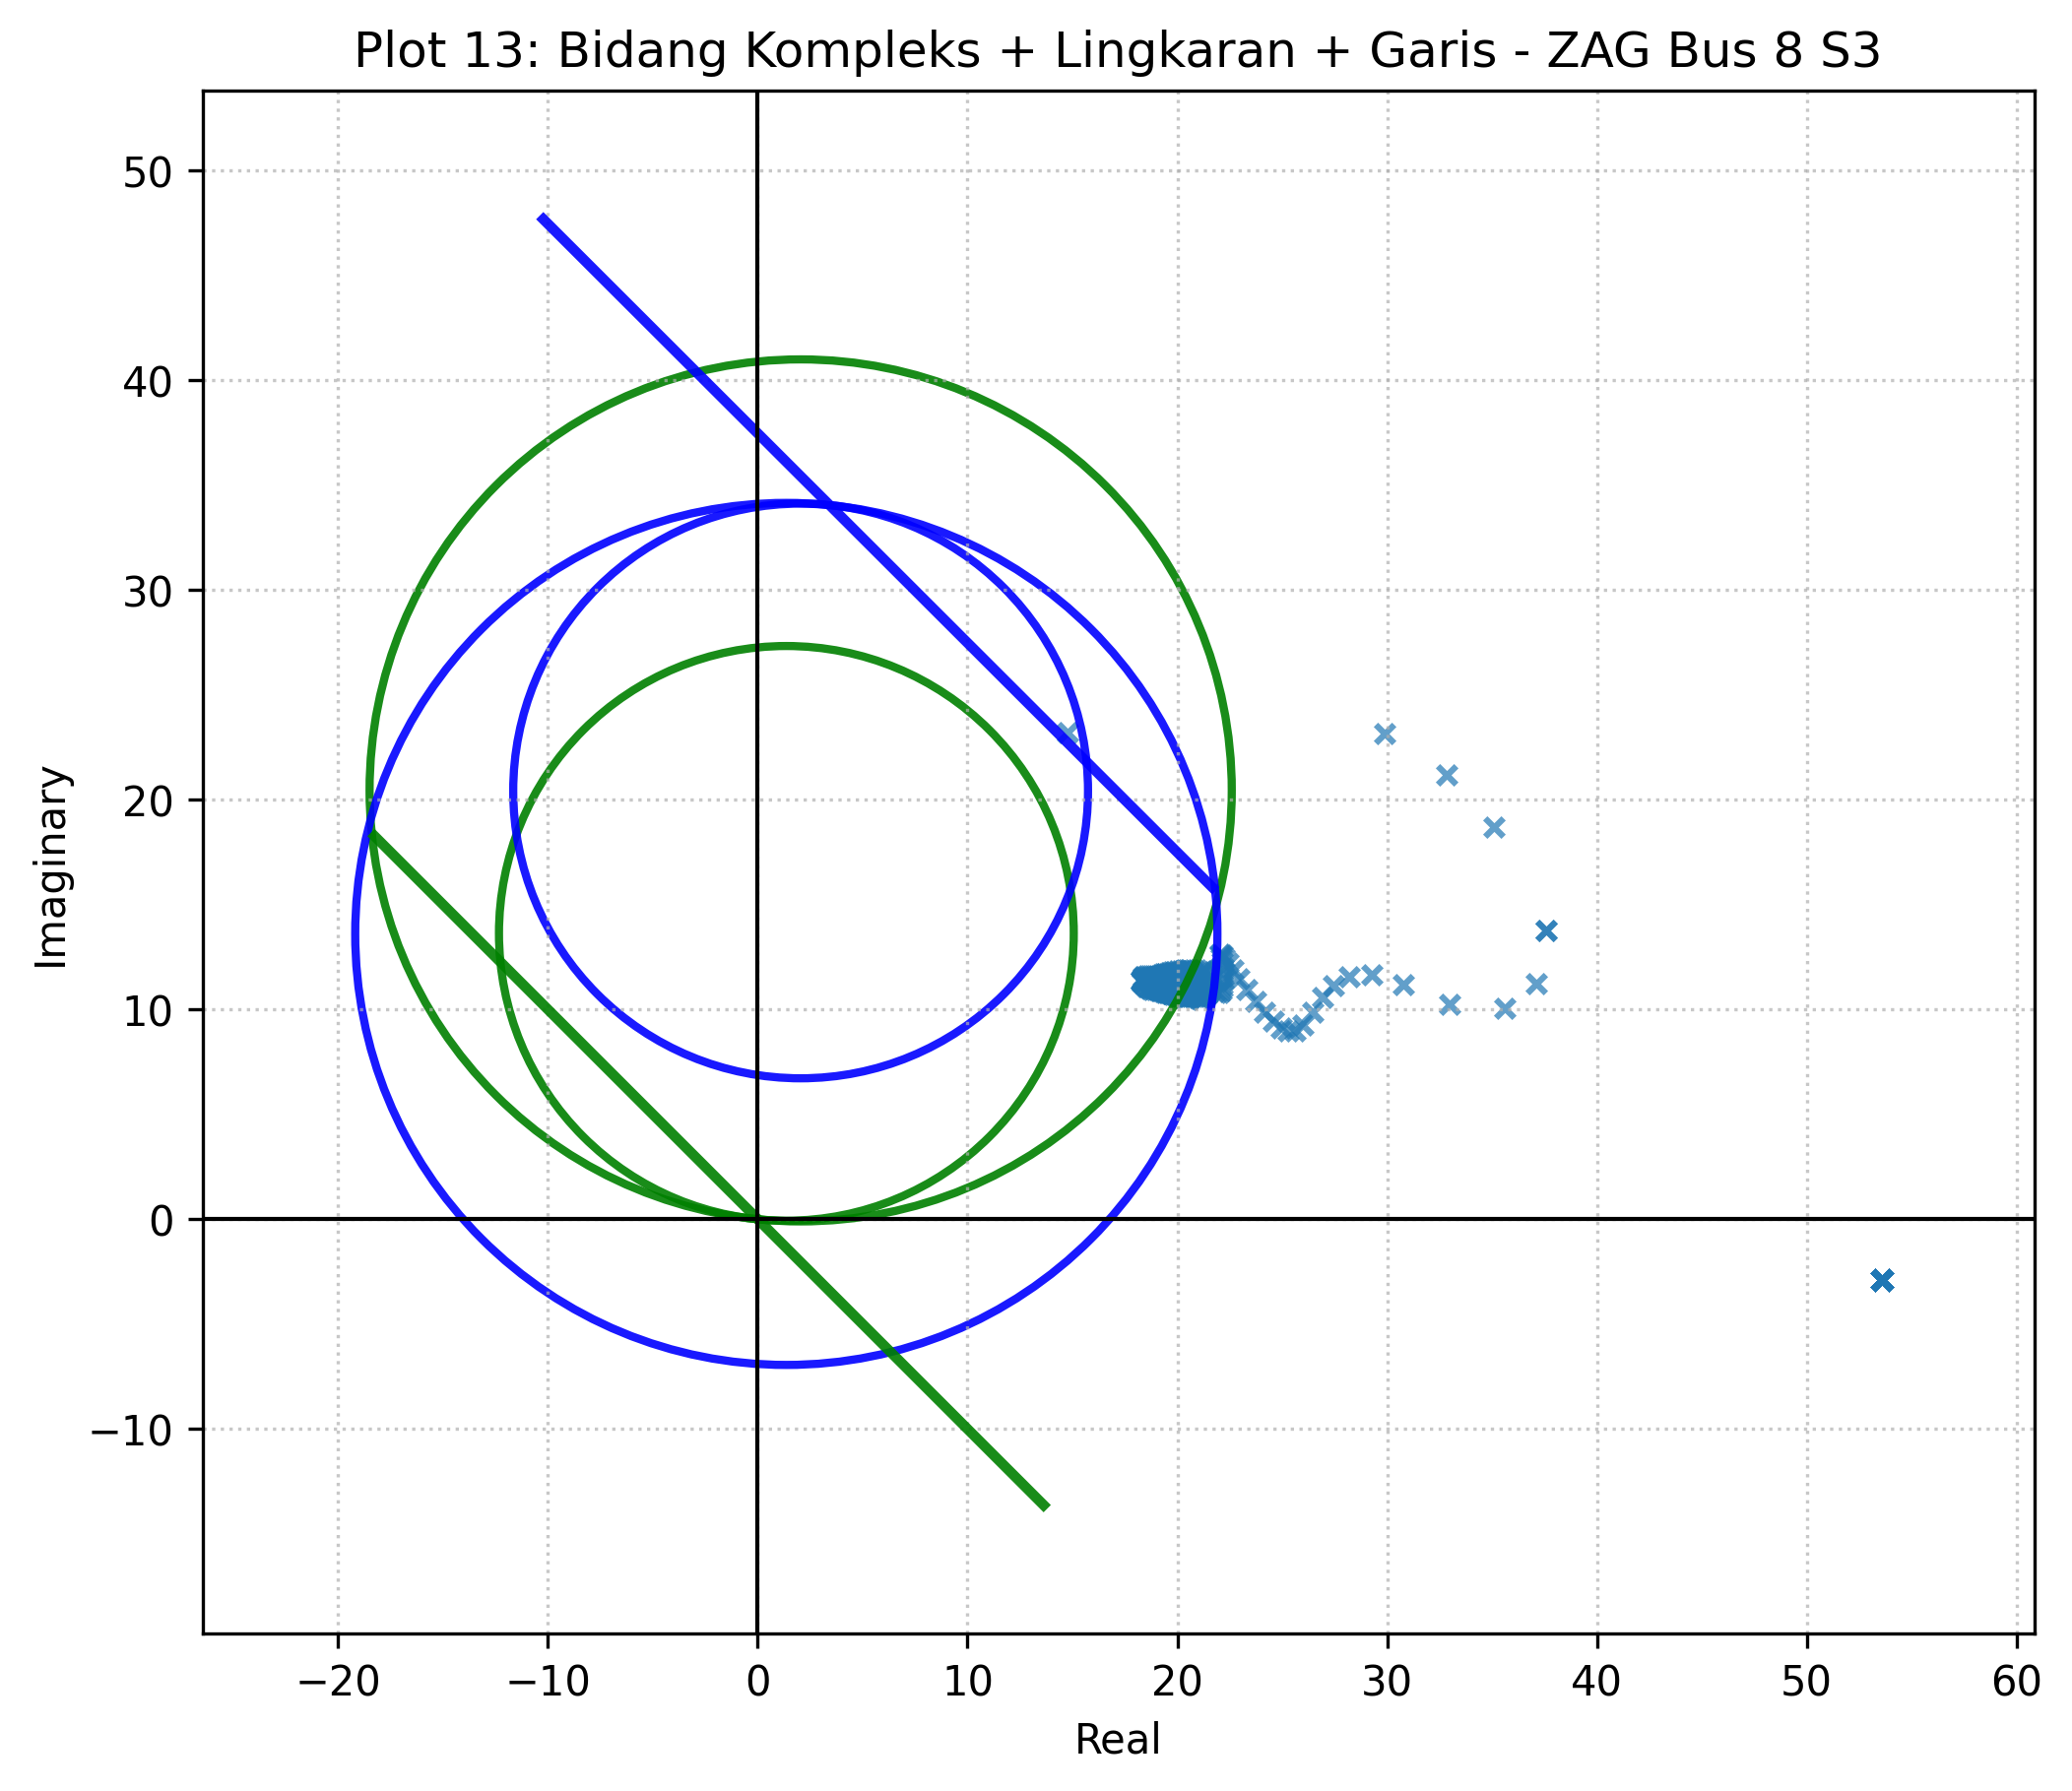
\includegraphics[width=0.8\textwidth]{contents/chapter-4/13_ZAG_Bus_8_S3_dengan_lingkaran_dan_garis.png}
%     \caption{Impedansi Tampak ZAG Bus 8 Skenario 3}
%     \label{fig:13_ZAG_Bus_8_S3_dengan_lingkaran_dan_garis}
% \end{figure}

% Terlihat pada gambar \ref{fig:13_ZAG_Bus_8_S3_dengan_lingkaran_dan_garis} bahwa impedansi tampak pada fasa A dengan ground yang dibaca oleh relay 21 sisi bus 8 saat terdapat gangguan mengalami over reach pada zona 1 serta mengalami drop out pada zona 2 sehingga dengan acuan pada \ref{subsec:tanpa_IBR_ex_dlg} relay 21 bus 8 mengalami missoperation trip pada zona 1.

%%%%%%%%%%%%%%%%%%%%%%%%%%%%%%%%%SISI PRIMER%%%%%%%%%%%%%%%%%%%%%%%%%%%%%%%%%%

\begin{figure}[H]
    \centering
    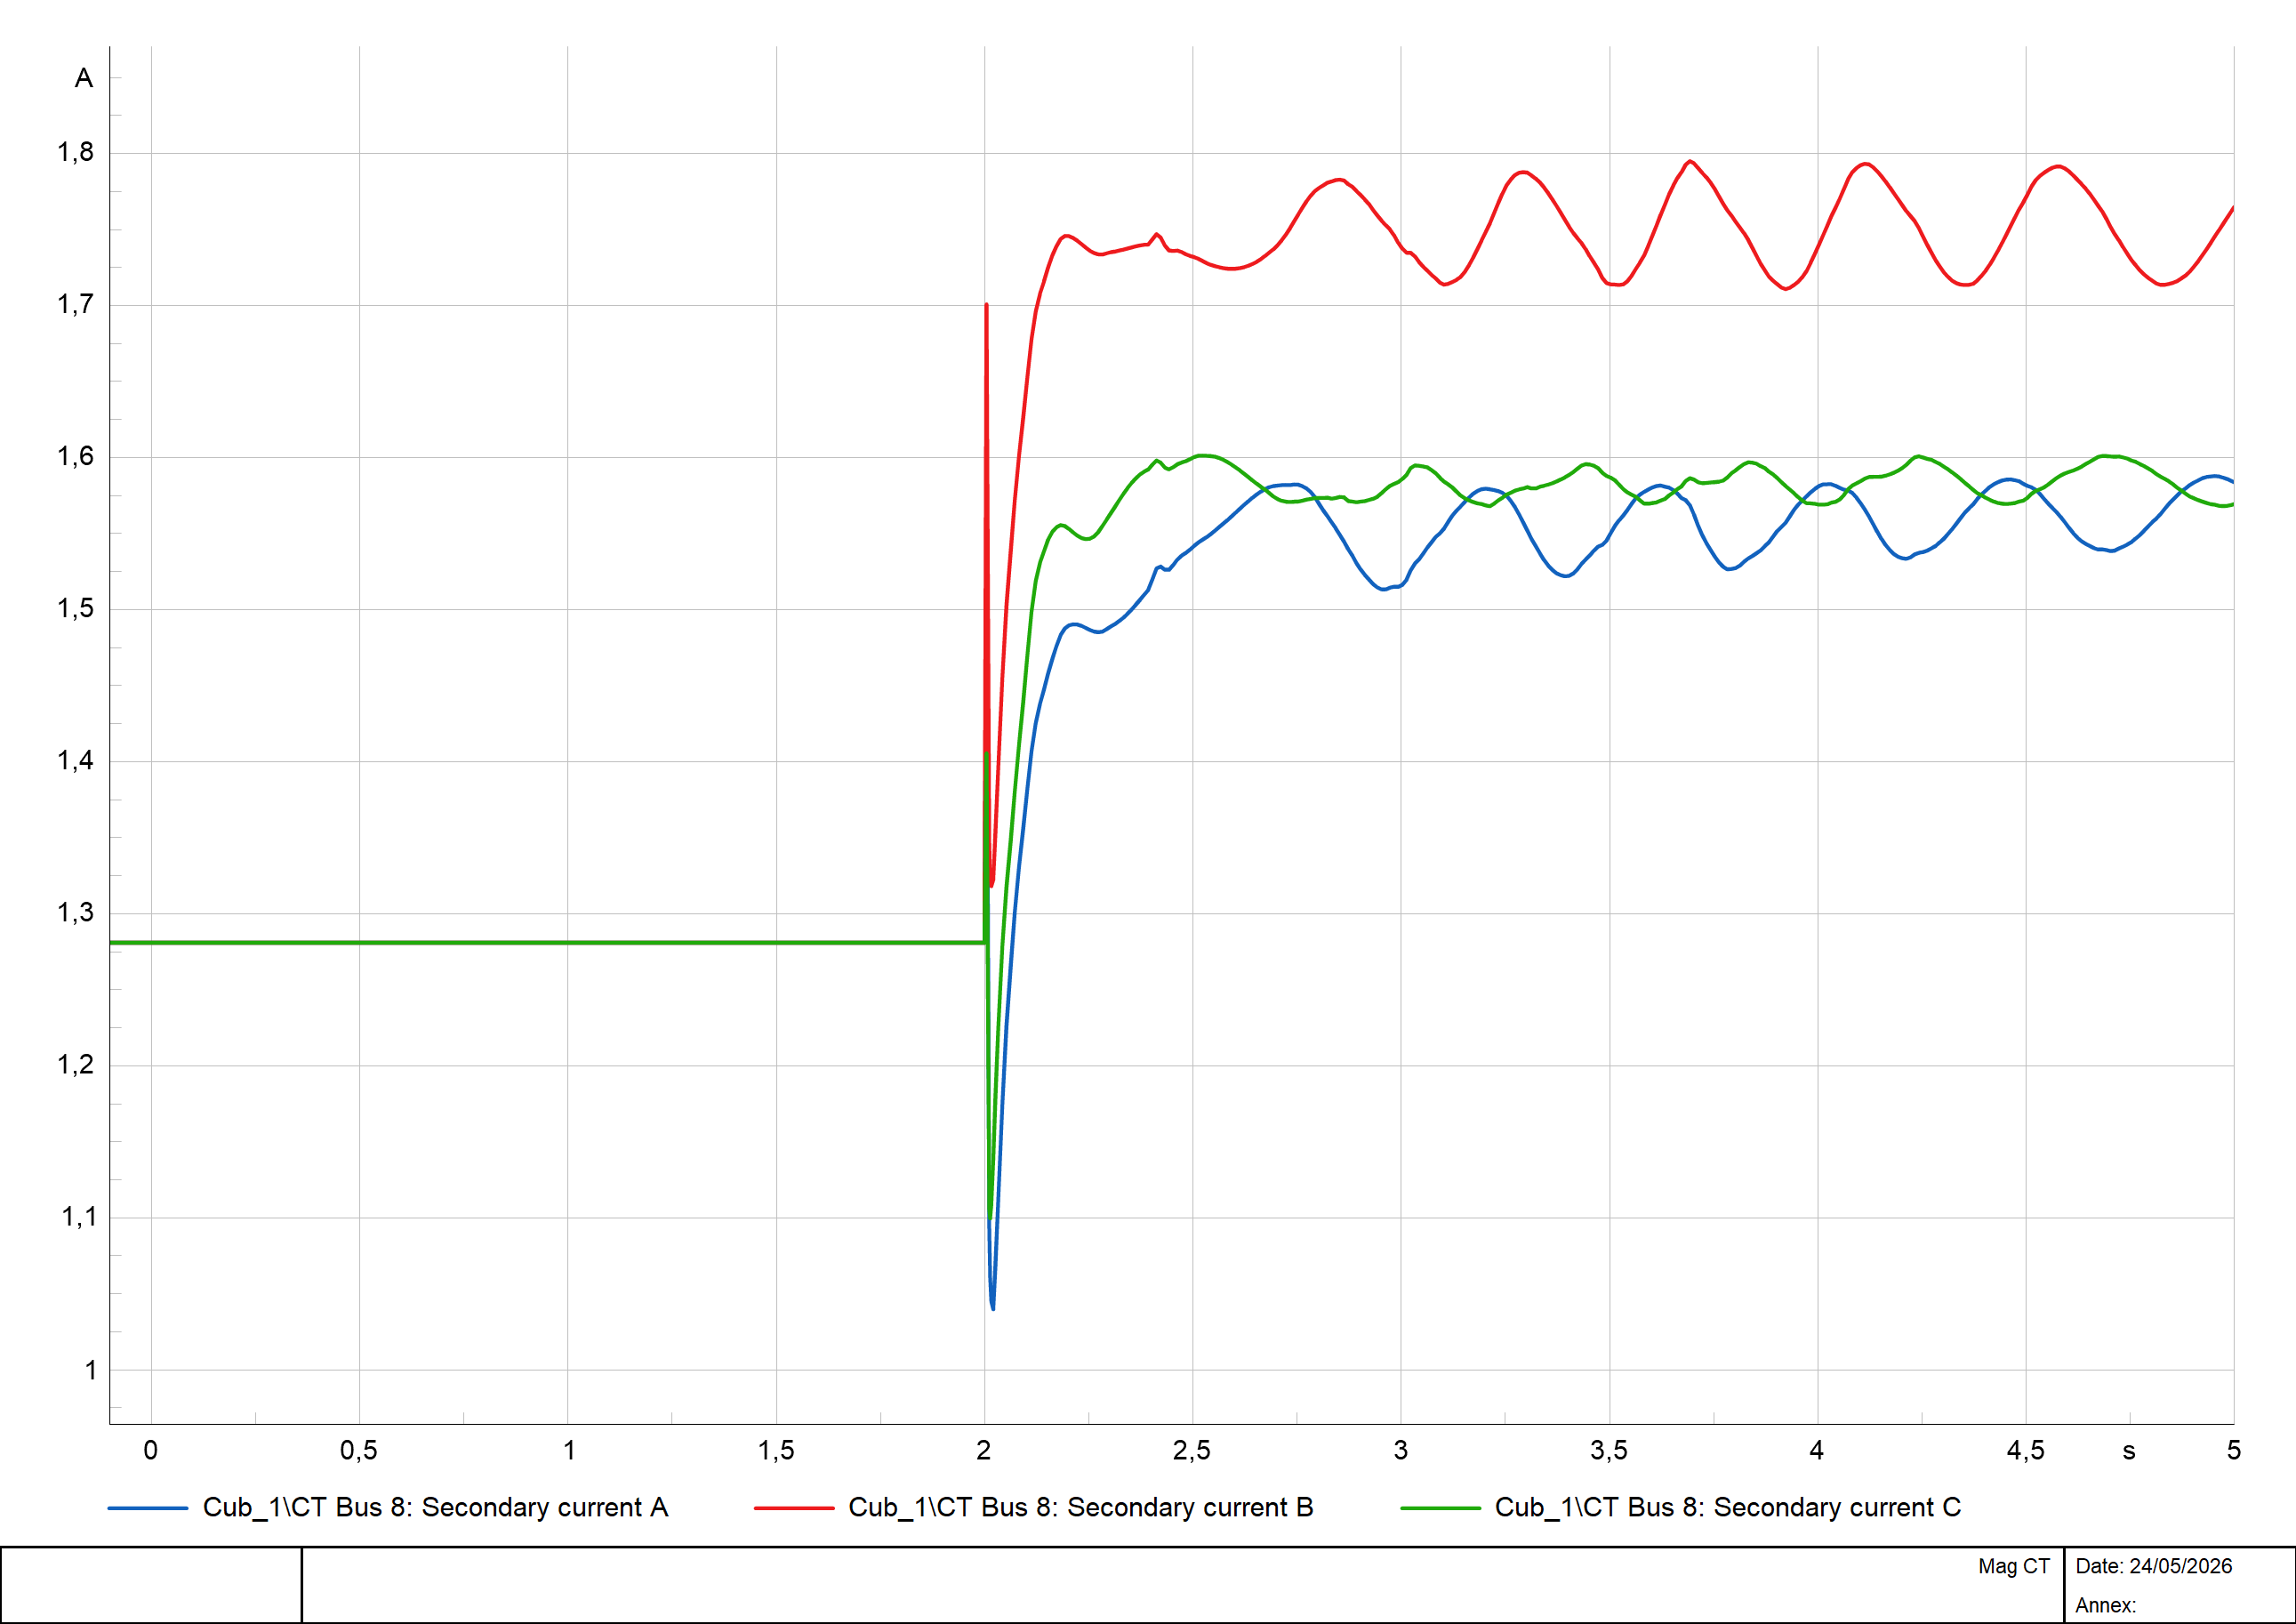
\includegraphics[width=0.8\textwidth]{contents/chapter-4/Bus_8_Ex_DLG_S3.png}
    \caption{Arus Sekunder CT Bus 8 Skenario 3}
    \label{fig:Bus_8_Ex_DLG_S3}
\end{figure}

Gambar \ref{fig:Bus_8_Ex_DLG_S3} menunjukkan arus sekunder CT pada Bus 8 untuk skenario 3. Sebelum gangguan, arus pada ketiga fasa berada pada nilai 1,281 A sekunder. Setelah gangguan terjadi, arus fasa A meningkat menjadi 1,601 A sekunder atau 1,25 p.u., arus fasa B meningkat menjadi 1,791 A sekunder atau 1,4 p.u., dan arus fasa C meningkat menjadi 1,586 A sekunder atau 1,24 p.u. Kenaikan arus tersebut menunjukkan adanya perubahan arus saat gangguan, tetapi nilainya masih belum memenuhi arus minimum yang diperlukan untuk membuat relay 21 sisi Bus 8 aktif.

\begin{figure}[H]
    \centering

    % Gambar sebelah kiri
    \begin{subfigure}[t]{0.48\textwidth}
        \centering
        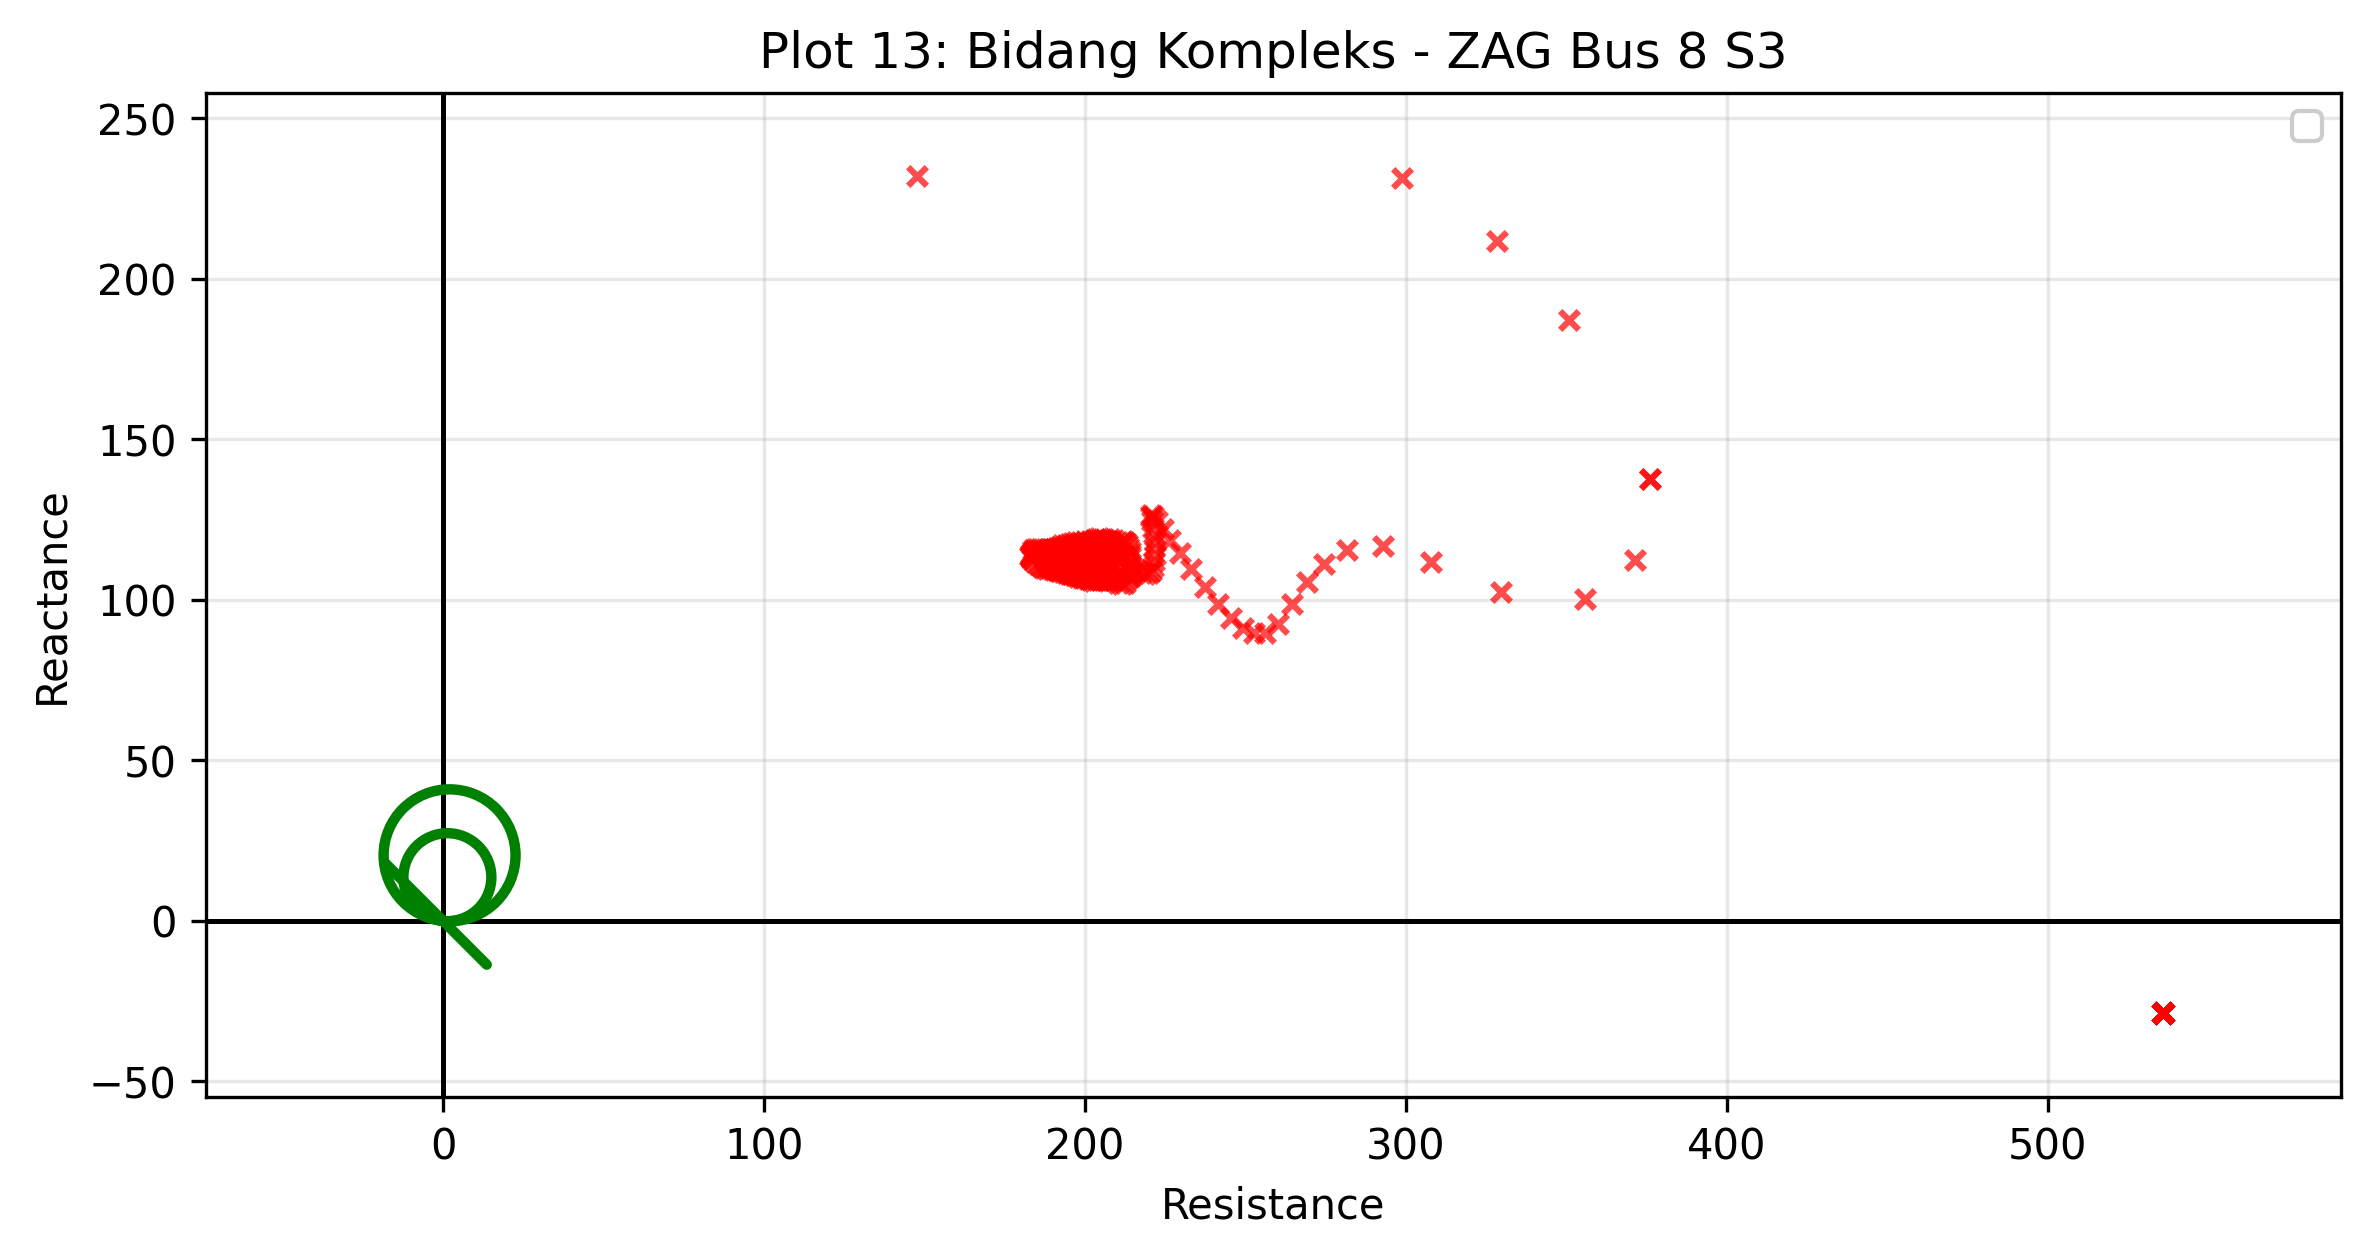
\includegraphics[width=\textwidth]{contents/chapter-4/PRIA_13_ZAG_Bus_8_S3.png}
        \caption{Seluruh Impedansi Tampak}
        \label{fig:PRIA_13_ZAG_Bus_8_S3}
    \end{subfigure}
    \hfill
    % Gambar sebelah kanan
    \begin{subfigure}[t]{0.48\textwidth}
        \centering
        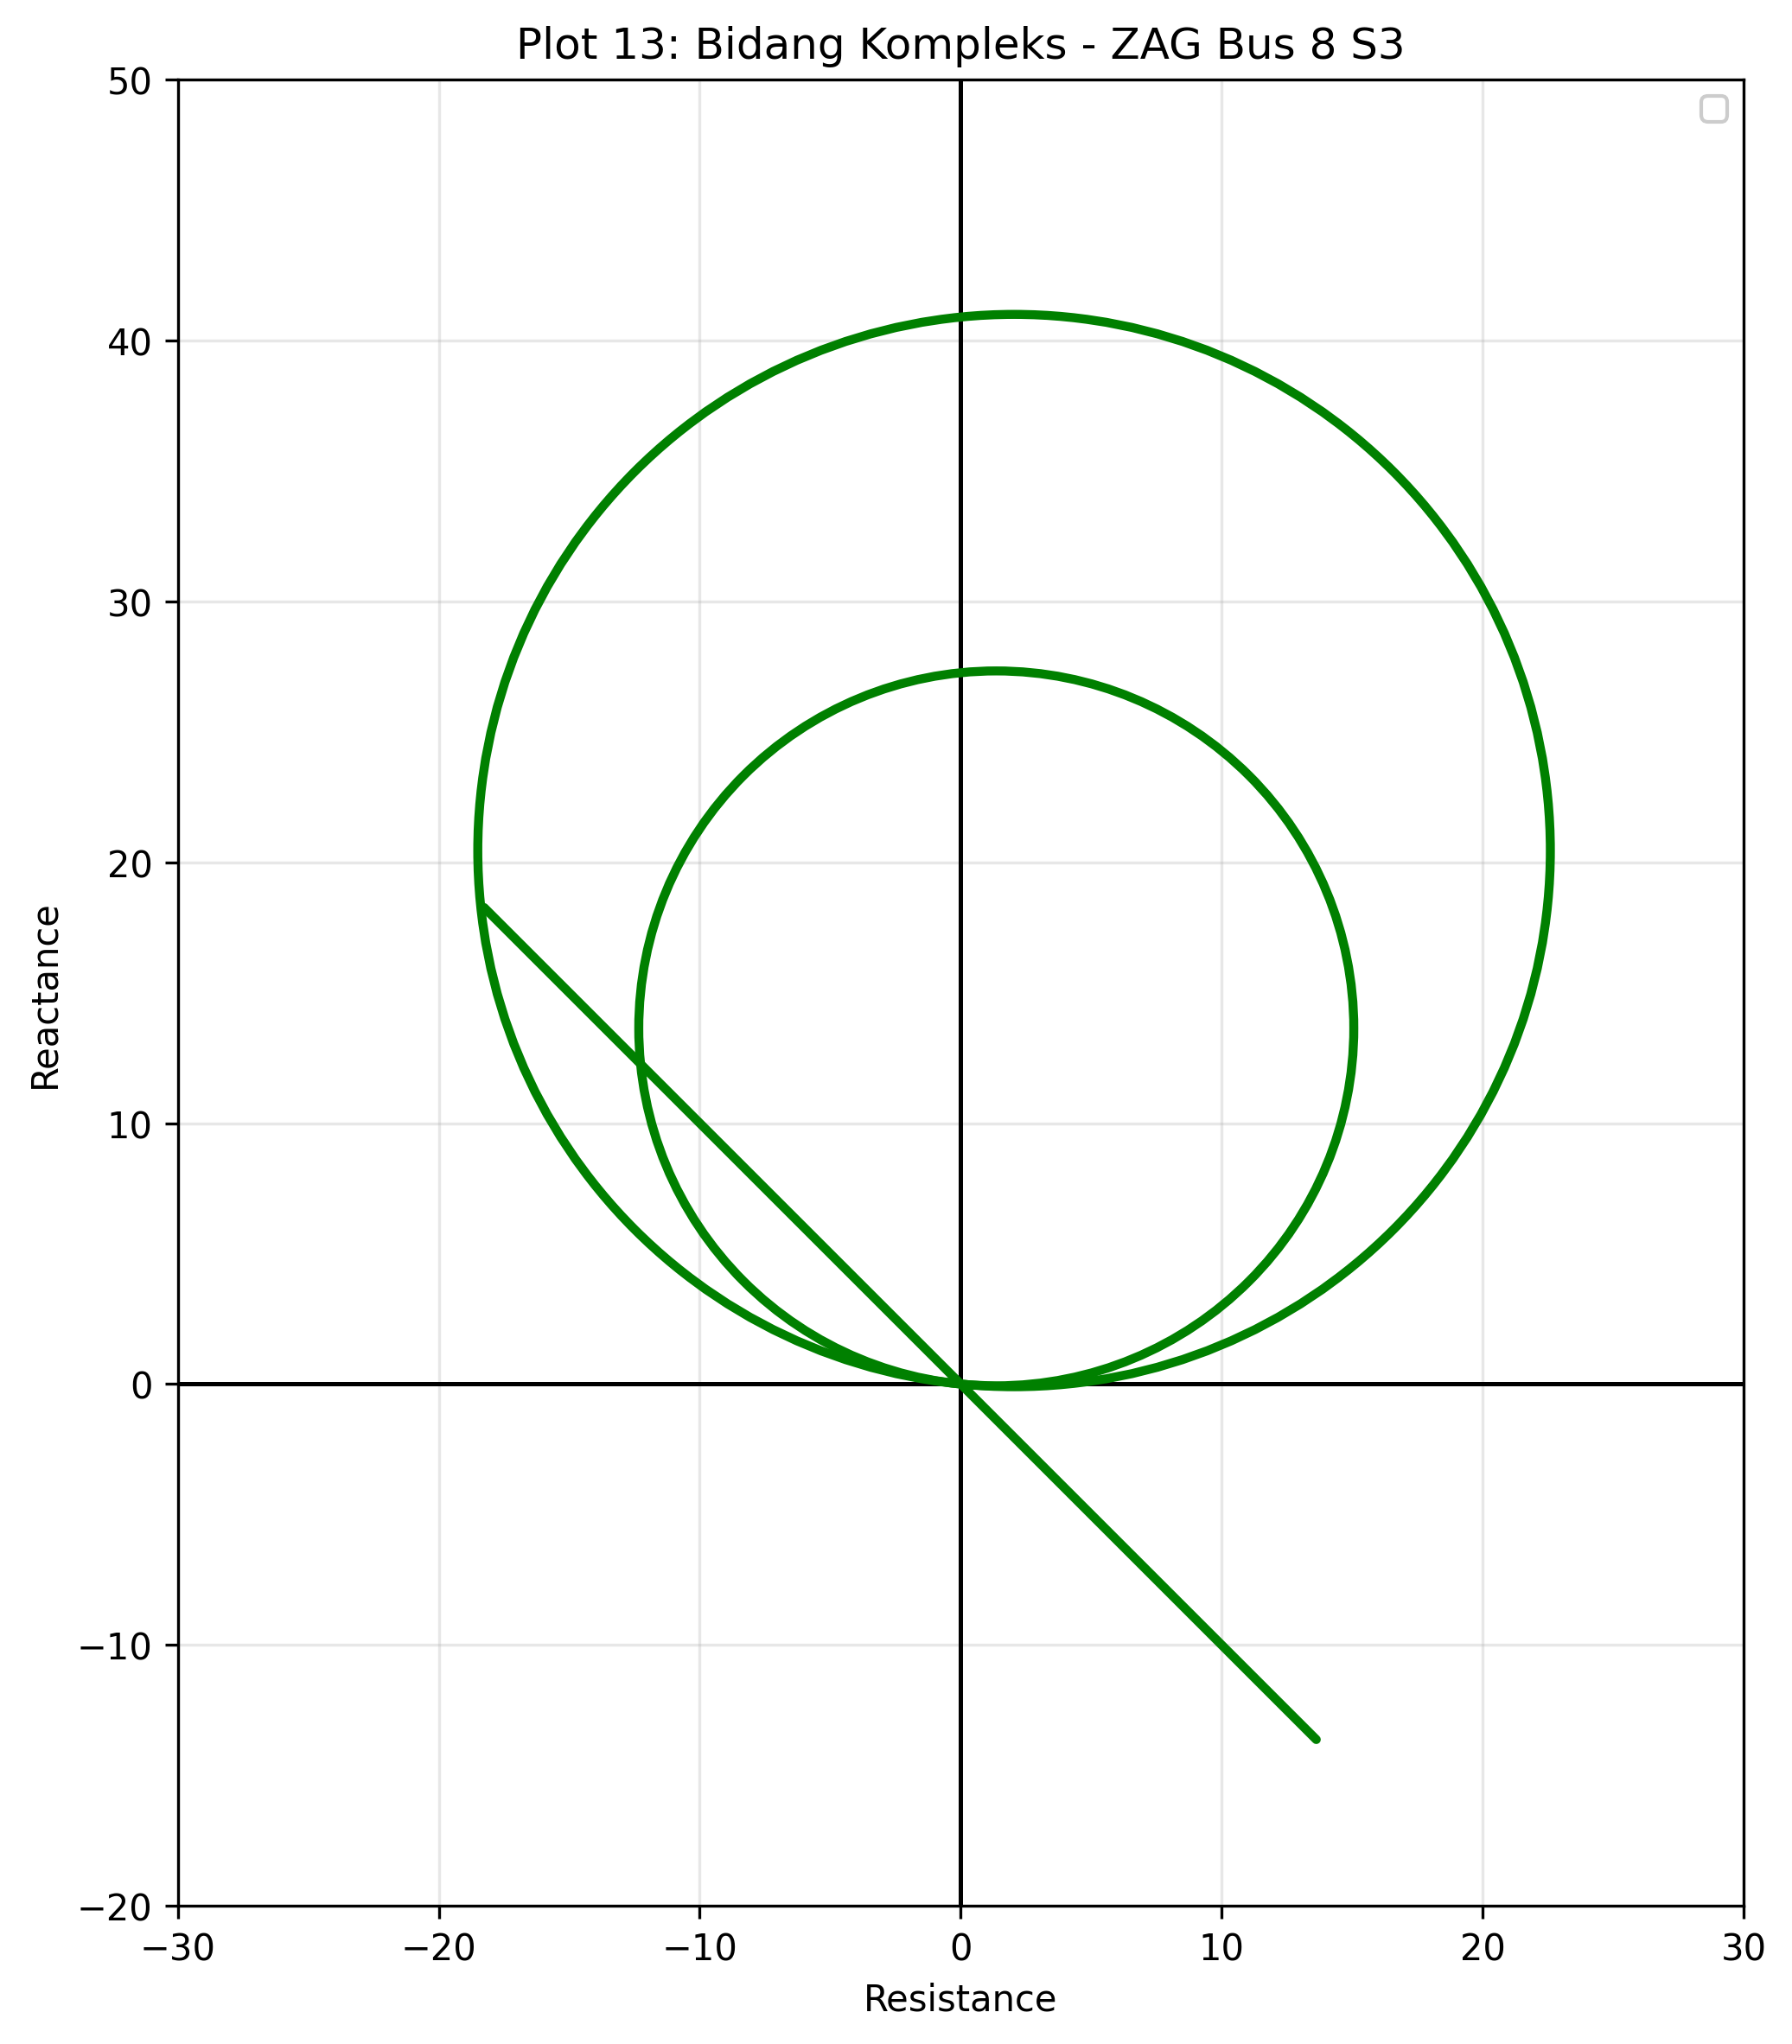
\includegraphics[width=\textwidth]{contents/chapter-4/PRIZI_13_ZAG_Bus_8_S3.png}
        \caption{Zoom In Pada Zona Proteksi}
        \label{fig:PRIZI_13_ZAG_Bus_8_S3}
    \end{subfigure}

    \caption{Impedansi Tampak ZAG Bus 8 Skenario 3}
    \label{fig:Impedansi_Tampak_ZAG_Bus_8_S3}
\end{figure}

Gambar \ref{fig:Impedansi_Tampak_ZAG_Bus_8_S3} menunjukkan bahwa impedansi tampak loop fasa A dengan ground yang dibaca oleh relay 21 sisi Bus 8 tidak masuk ke dalam zona proteksi. Kondisi ini sejalan dengan pembacaan arus sekunder CT pada Gambar \ref{fig:Bus_8_Ex_DLG_S3}, karena arus yang terbaca tidak memenuhi arus minimum untuk membuat relay aktif. Dengan mengacu pada kondisi dasar gangguan eksternal DLG pada Subbab \ref{subsec:tanpa_IBR_ex_dlg}, respons relay 21 sisi Bus 8 pada elemen ini dikategorikan mengalami \textit{misoperation}.

%%%%%%%%%%%%%%%%%%%%%%%%%%%%%%%%%%%%%%%%%%%%%%%%%%%%%%%%%%%%%%%


% \begin{figure}[H]
%     \centering
%     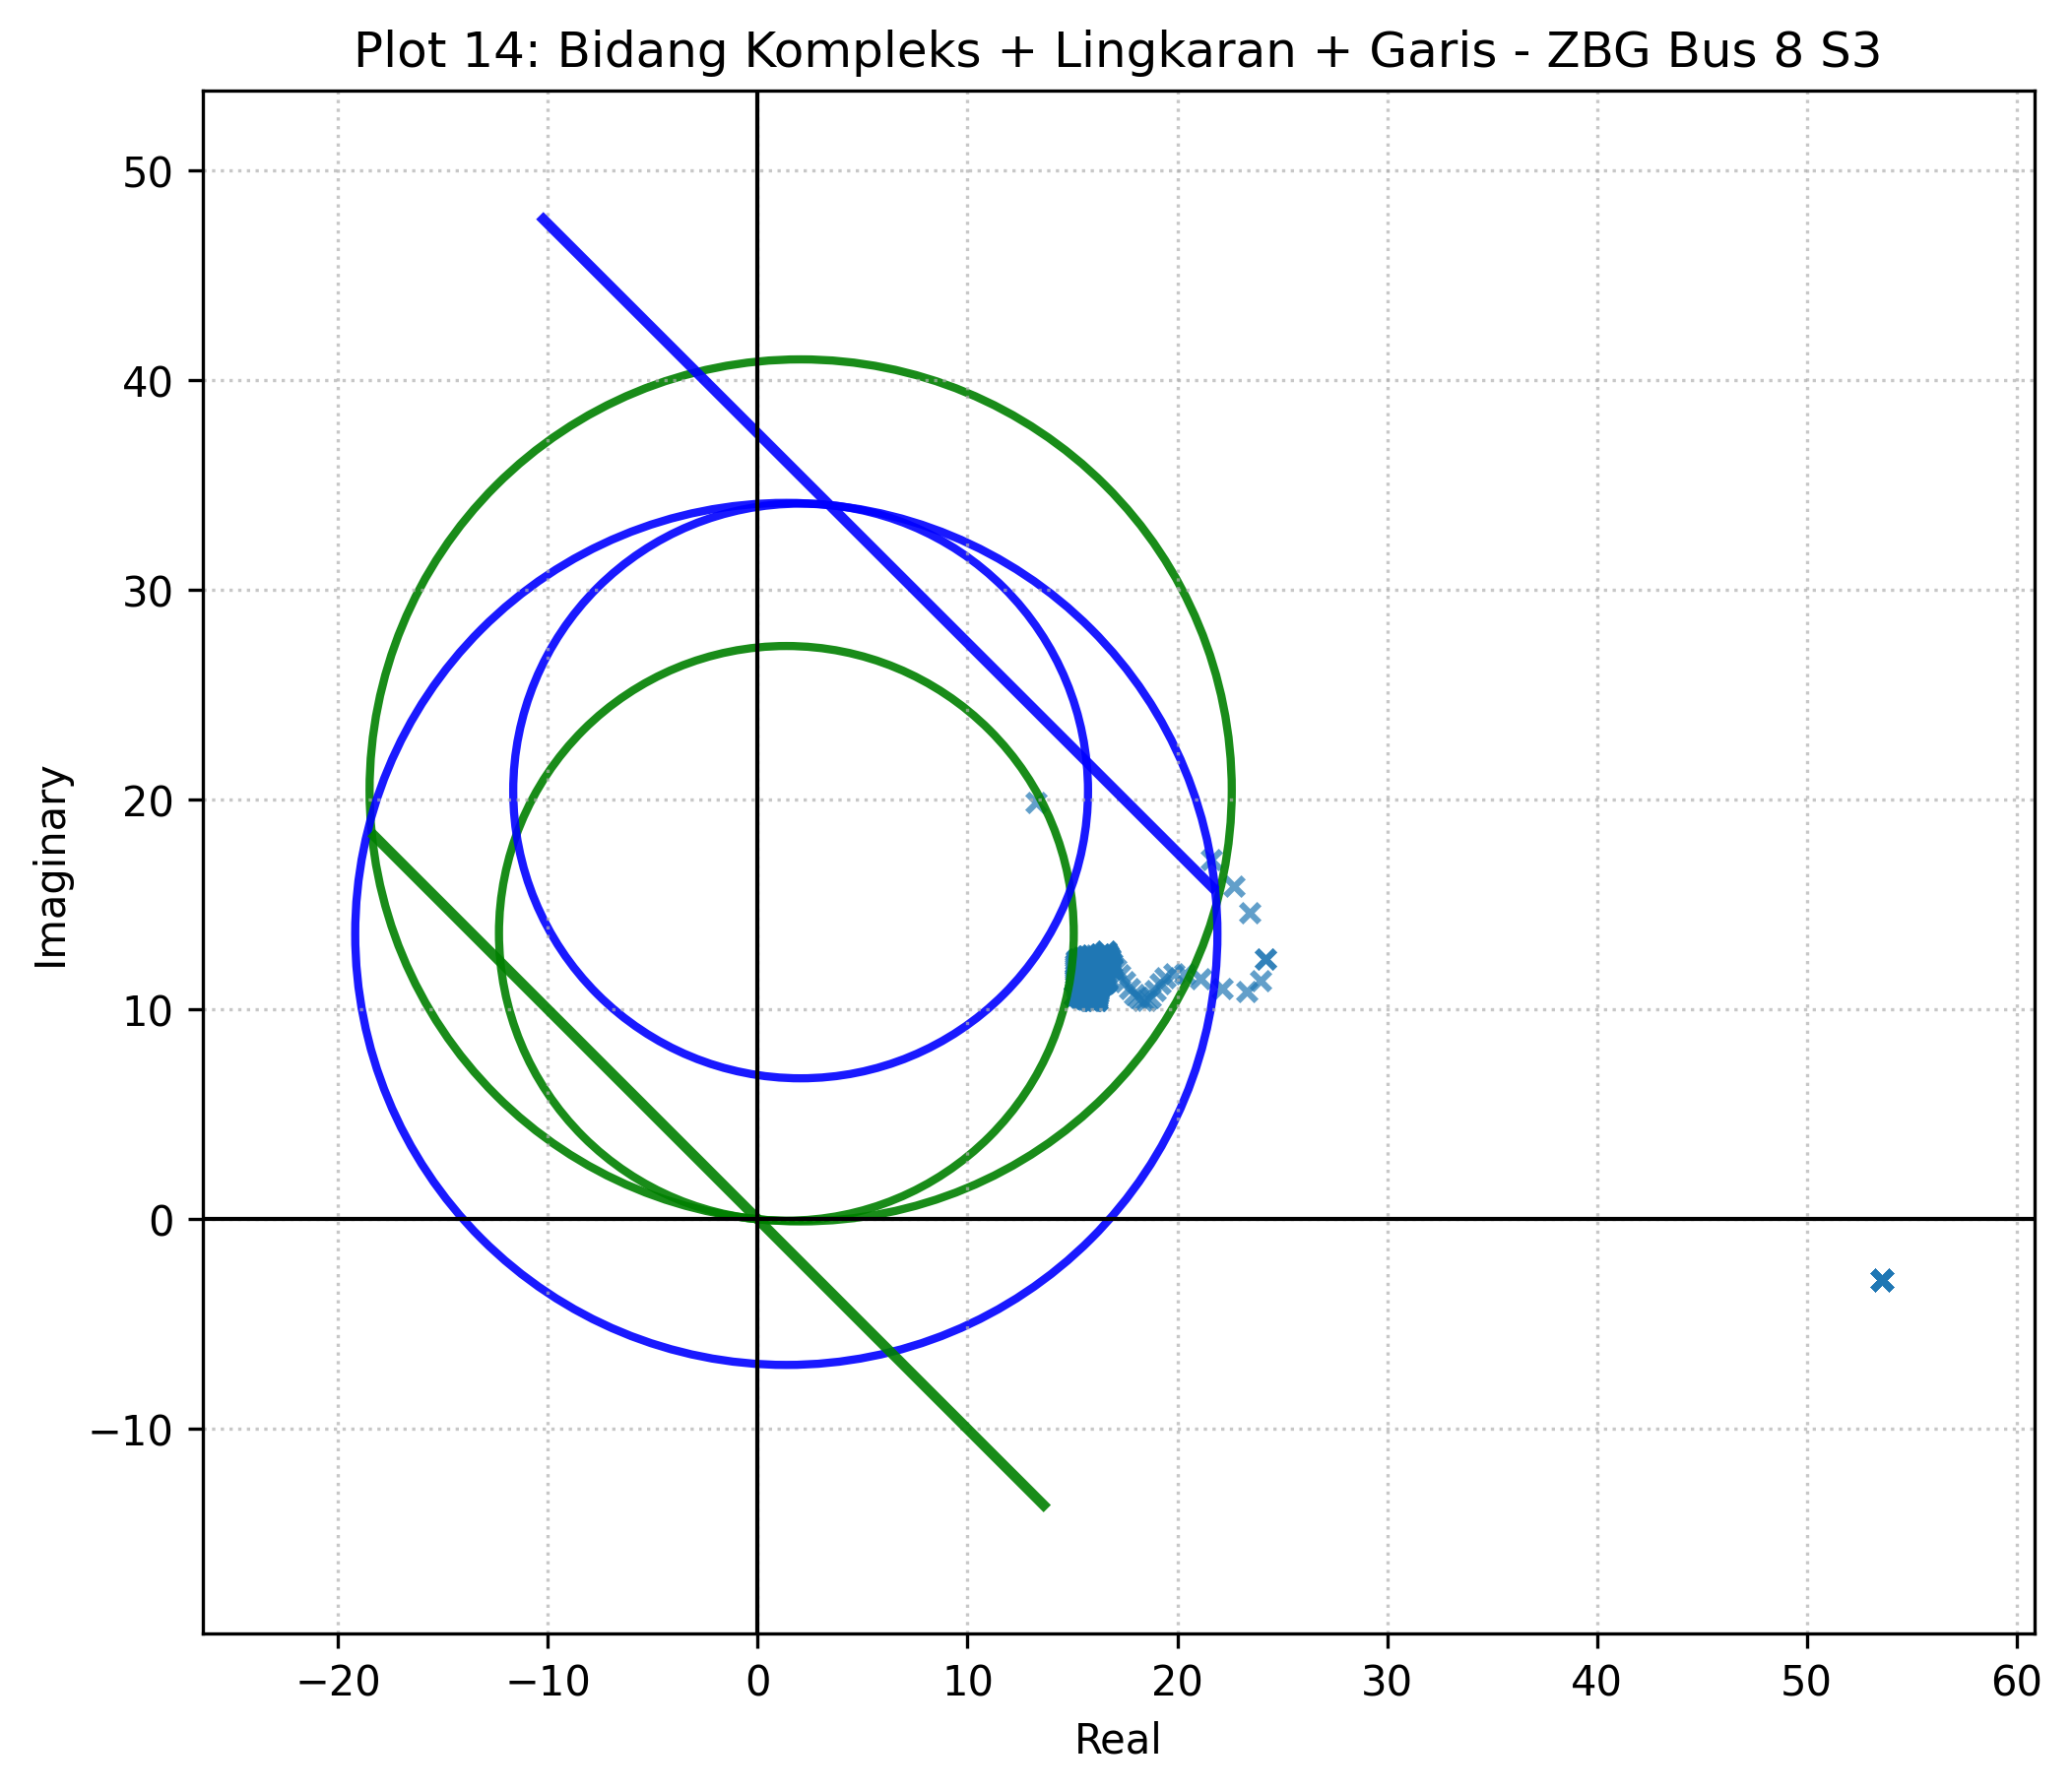
\includegraphics[width=0.8\textwidth]{contents/chapter-4/14_ZBG_Bus_8_S3_dengan_lingkaran_dan_garis.png}
%     \caption{Impedansi Tampak ZBG Bus 8 Skenario 3}
%     \label{fig:14_ZBG_Bus_8_S3_dengan_lingkaran_dan_garis}
% \end{figure}

% Terlihat pada gambar \ref{fig:14_ZBG_Bus_8_S3_dengan_lingkaran_dan_garis} bahwa impedansi tampak pada fasa B dengan ground yang dibaca oleh relay 21 sisi bus 8 saat terdapat gangguan mengalami over reach pada zona 1 serta mengalami drop out pada zona 2 sehingga dengan acuan pada \ref{subsec:tanpa_IBR_ex_dlg} relay 21 bus 8 mengalami missoperation trip pada zona 1.

%%%%%%%%%%%%%%%%%%%%%%%%%%%%%%%%%SISI PRIMER%%%%%%%%%%%%%%%%%%%%%%%%%%%%%%%%%%

% \begin{figure}[H]
%     \centering
%     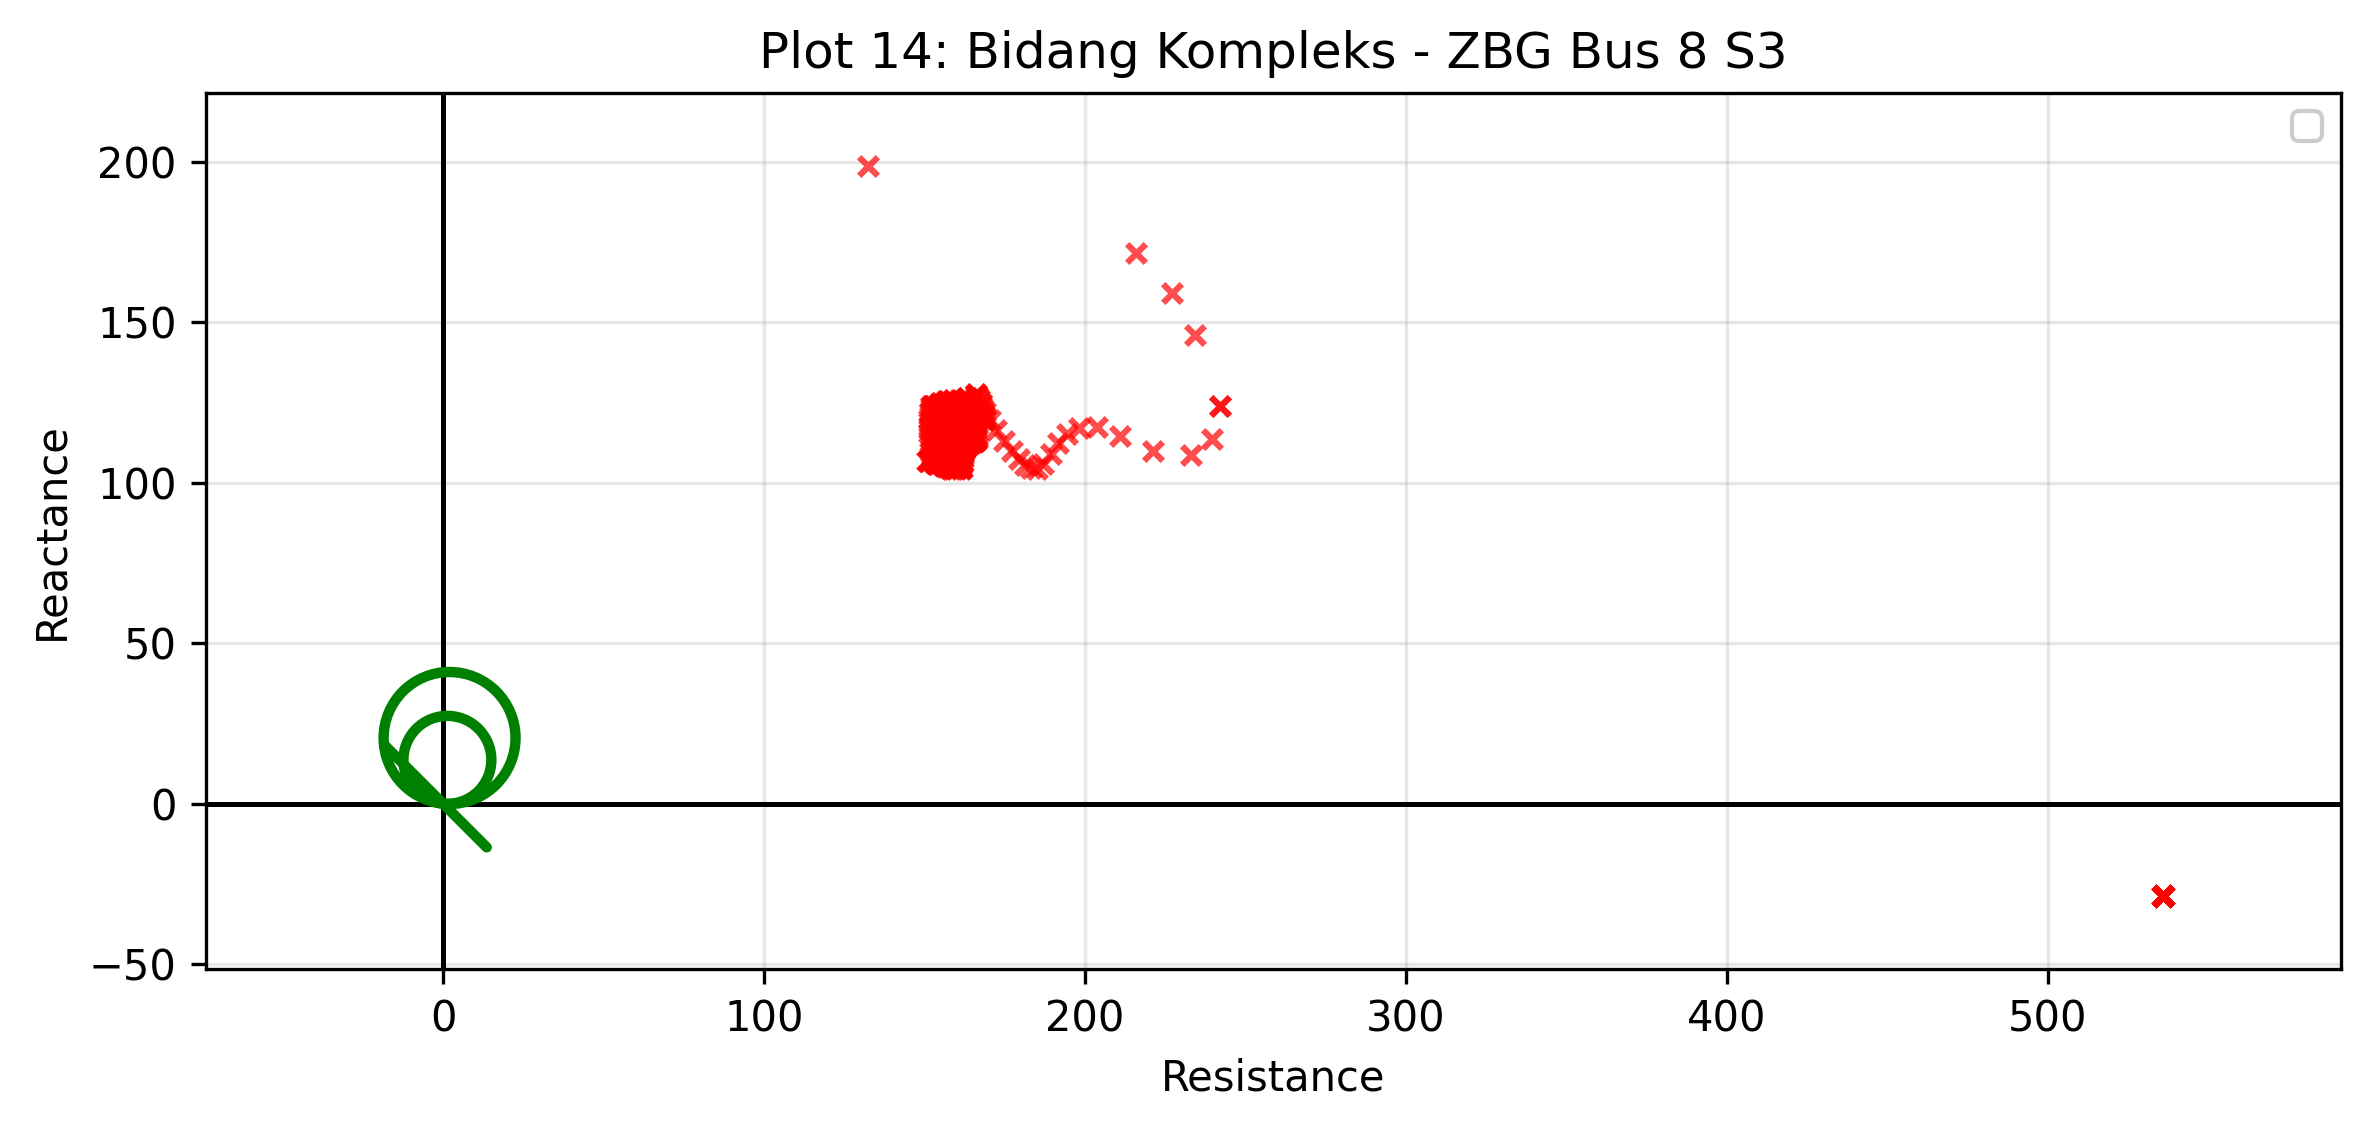
\includegraphics[width=0.8\textwidth]{contents/chapter-4/PRIA_14_ZBG_Bus_8_S3.png}
%     \caption{Impedansi Tampak ZBG Bus 8 Skenario 3}
%     \label{fig:PRIA_14_ZBG_Bus_8_S3}
% \end{figure}

% \begin{figure}[H]
%     \centering
%     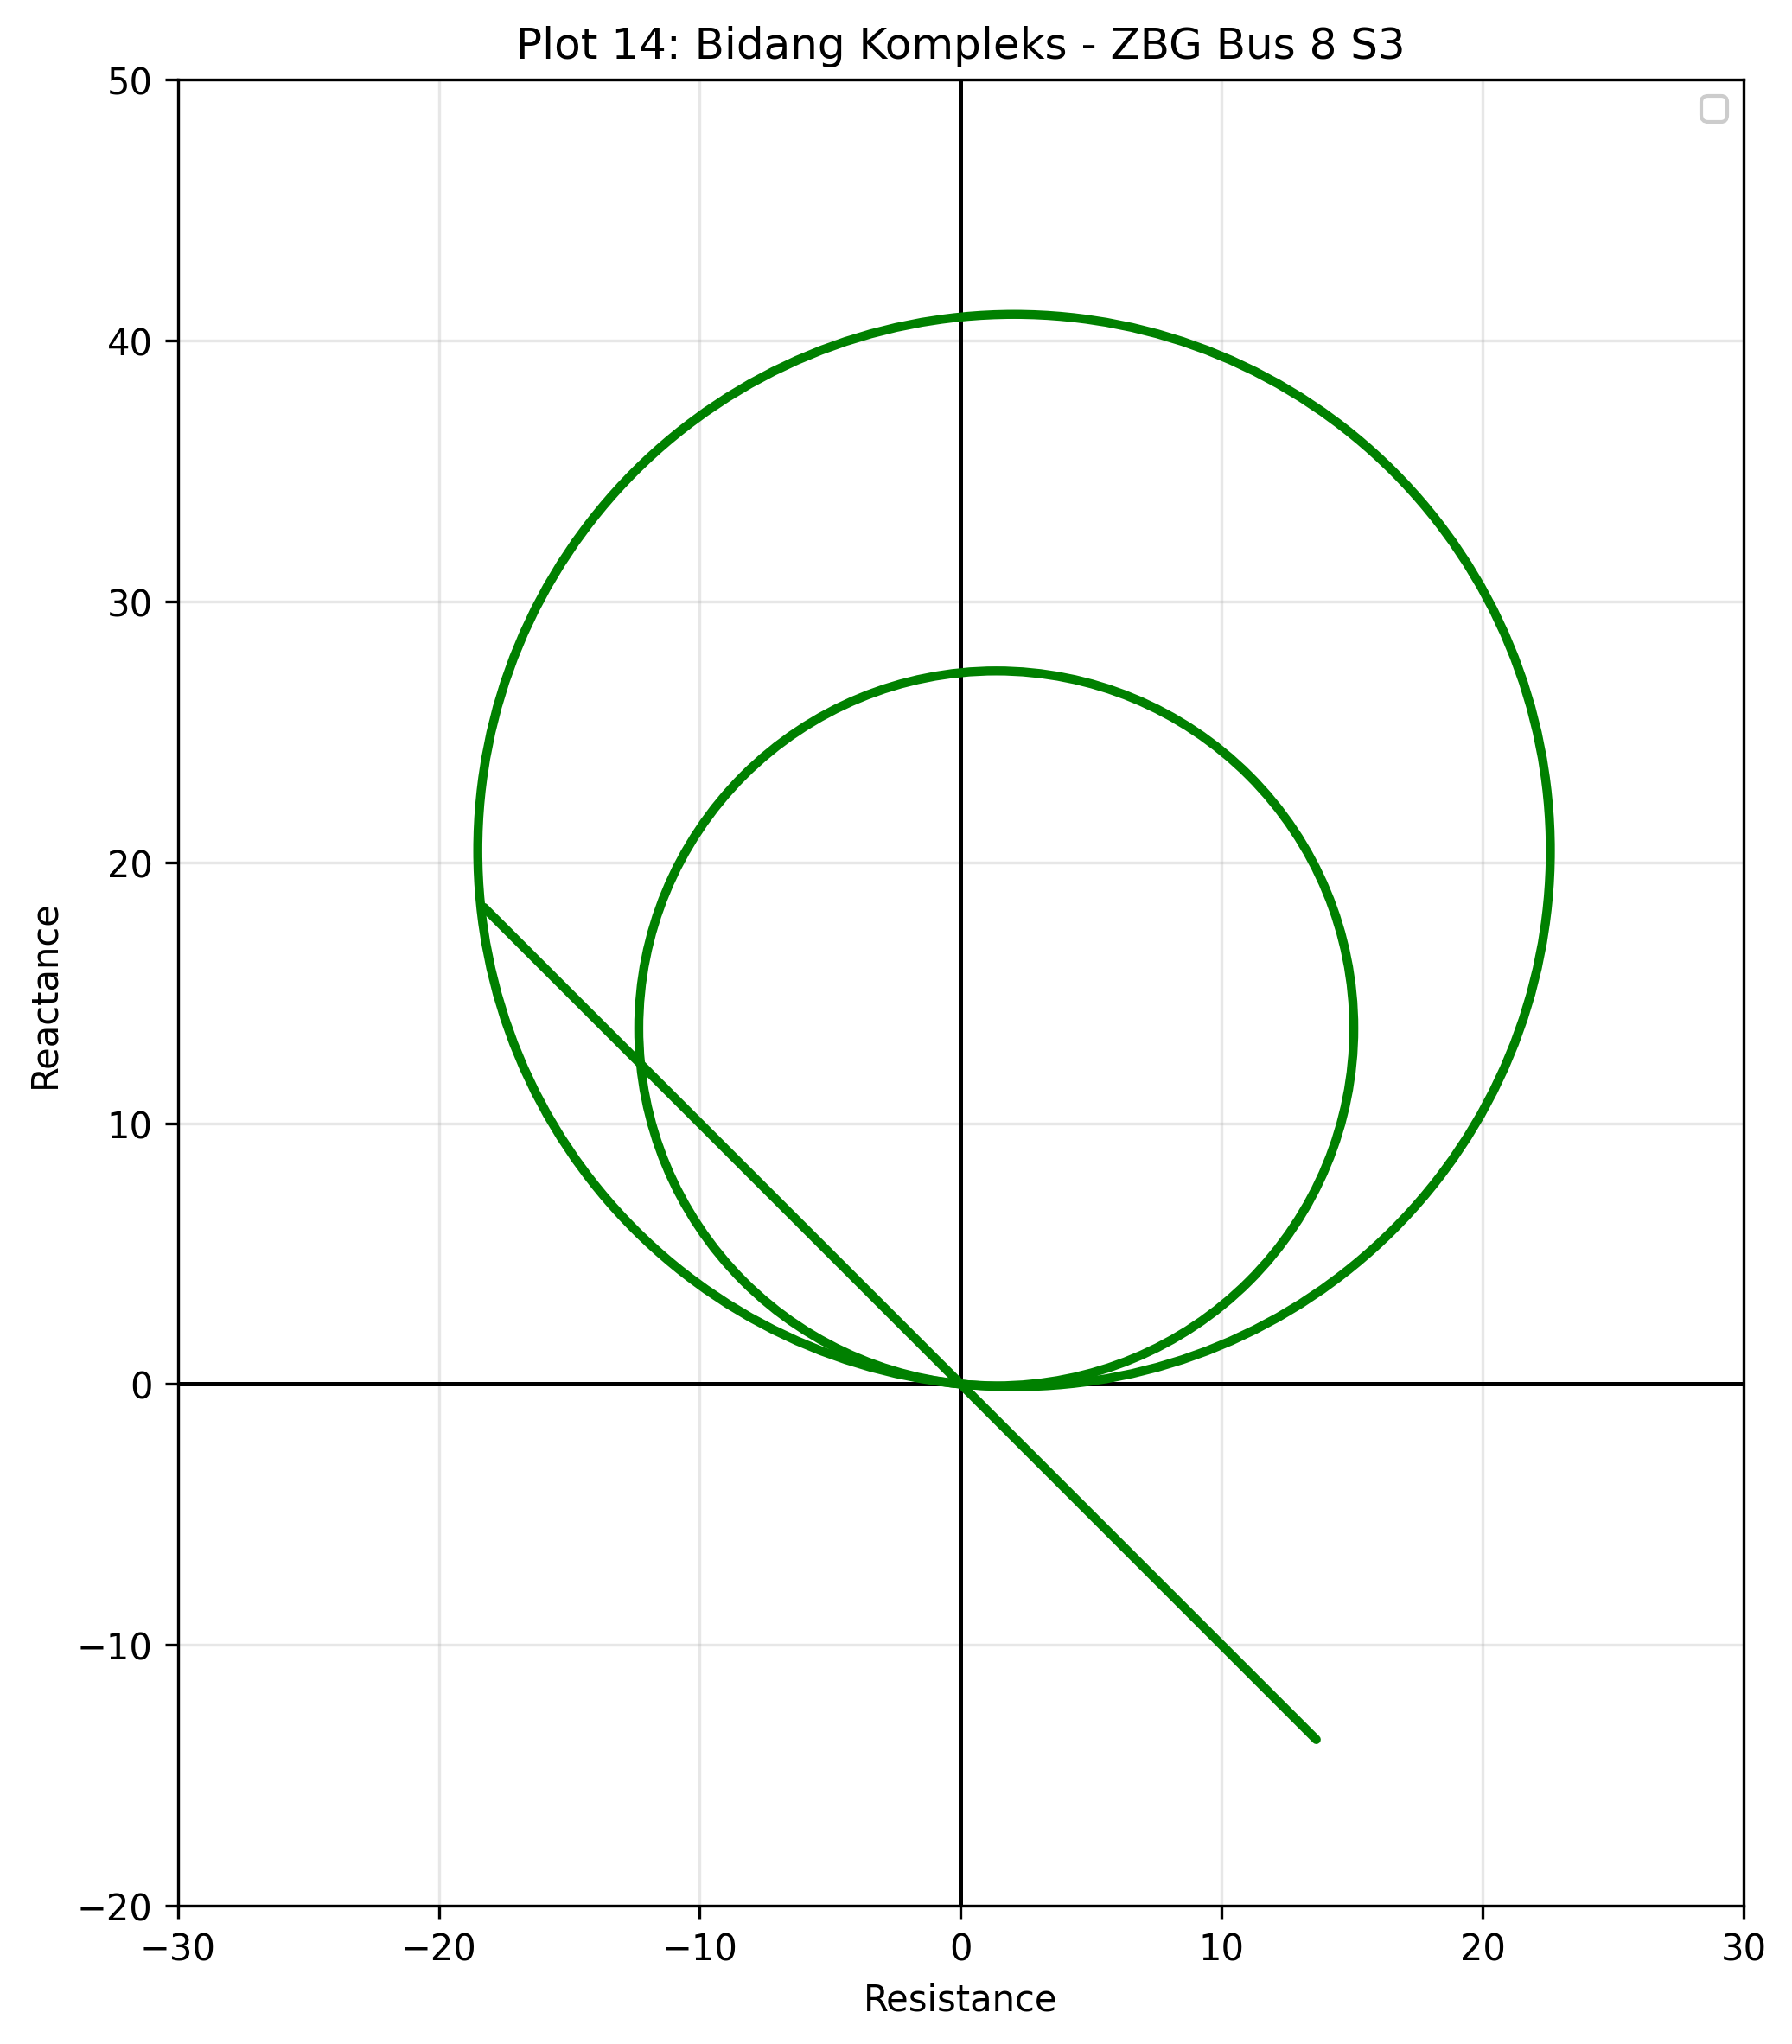
\includegraphics[width=0.8\textwidth]{contents/chapter-4/PRIZI_14_ZBG_Bus_8_S3.png}
%     \caption{Impedansi Tampak ZBG Bus 8 Skenario 3}
%     \label{fig:PRIZI_14_ZBG_Bus_8_S3}
% \end{figure}

\begin{figure}[H]
    \centering

    % Gambar sebelah kiri
    \begin{subfigure}[t]{0.48\textwidth}
        \centering
        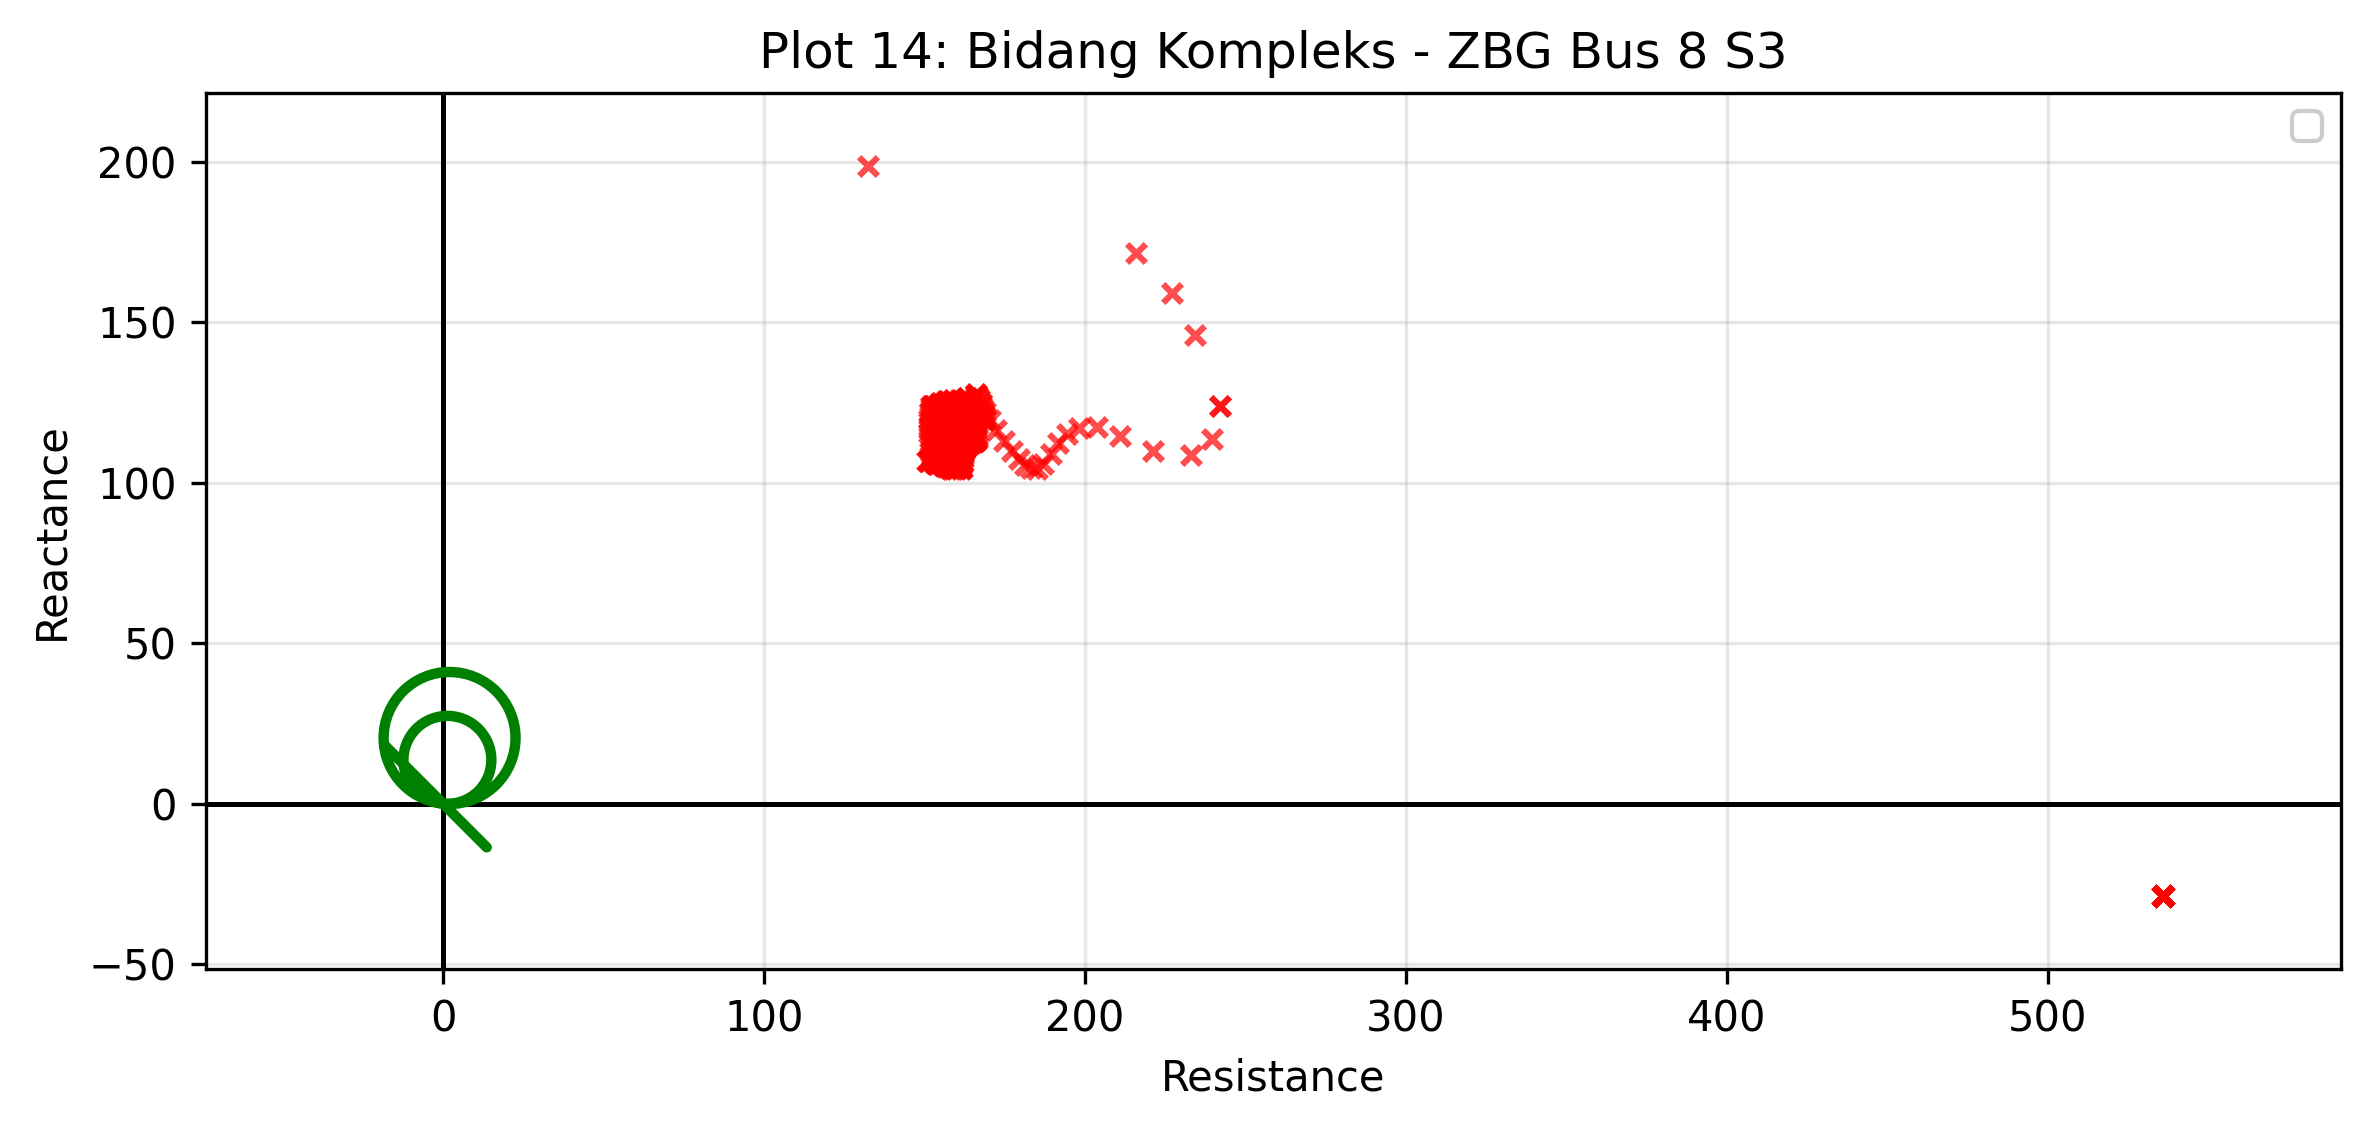
\includegraphics[width=\textwidth]{contents/chapter-4/PRIA_14_ZBG_Bus_8_S3.png}
        \caption{Seluruh Impedansi Tampak}
        \label{fig:PRIA_14_ZBG_Bus_8_S3}
    \end{subfigure}
    \hfill
    % Gambar sebelah kanan
    \begin{subfigure}[t]{0.48\textwidth}
        \centering
        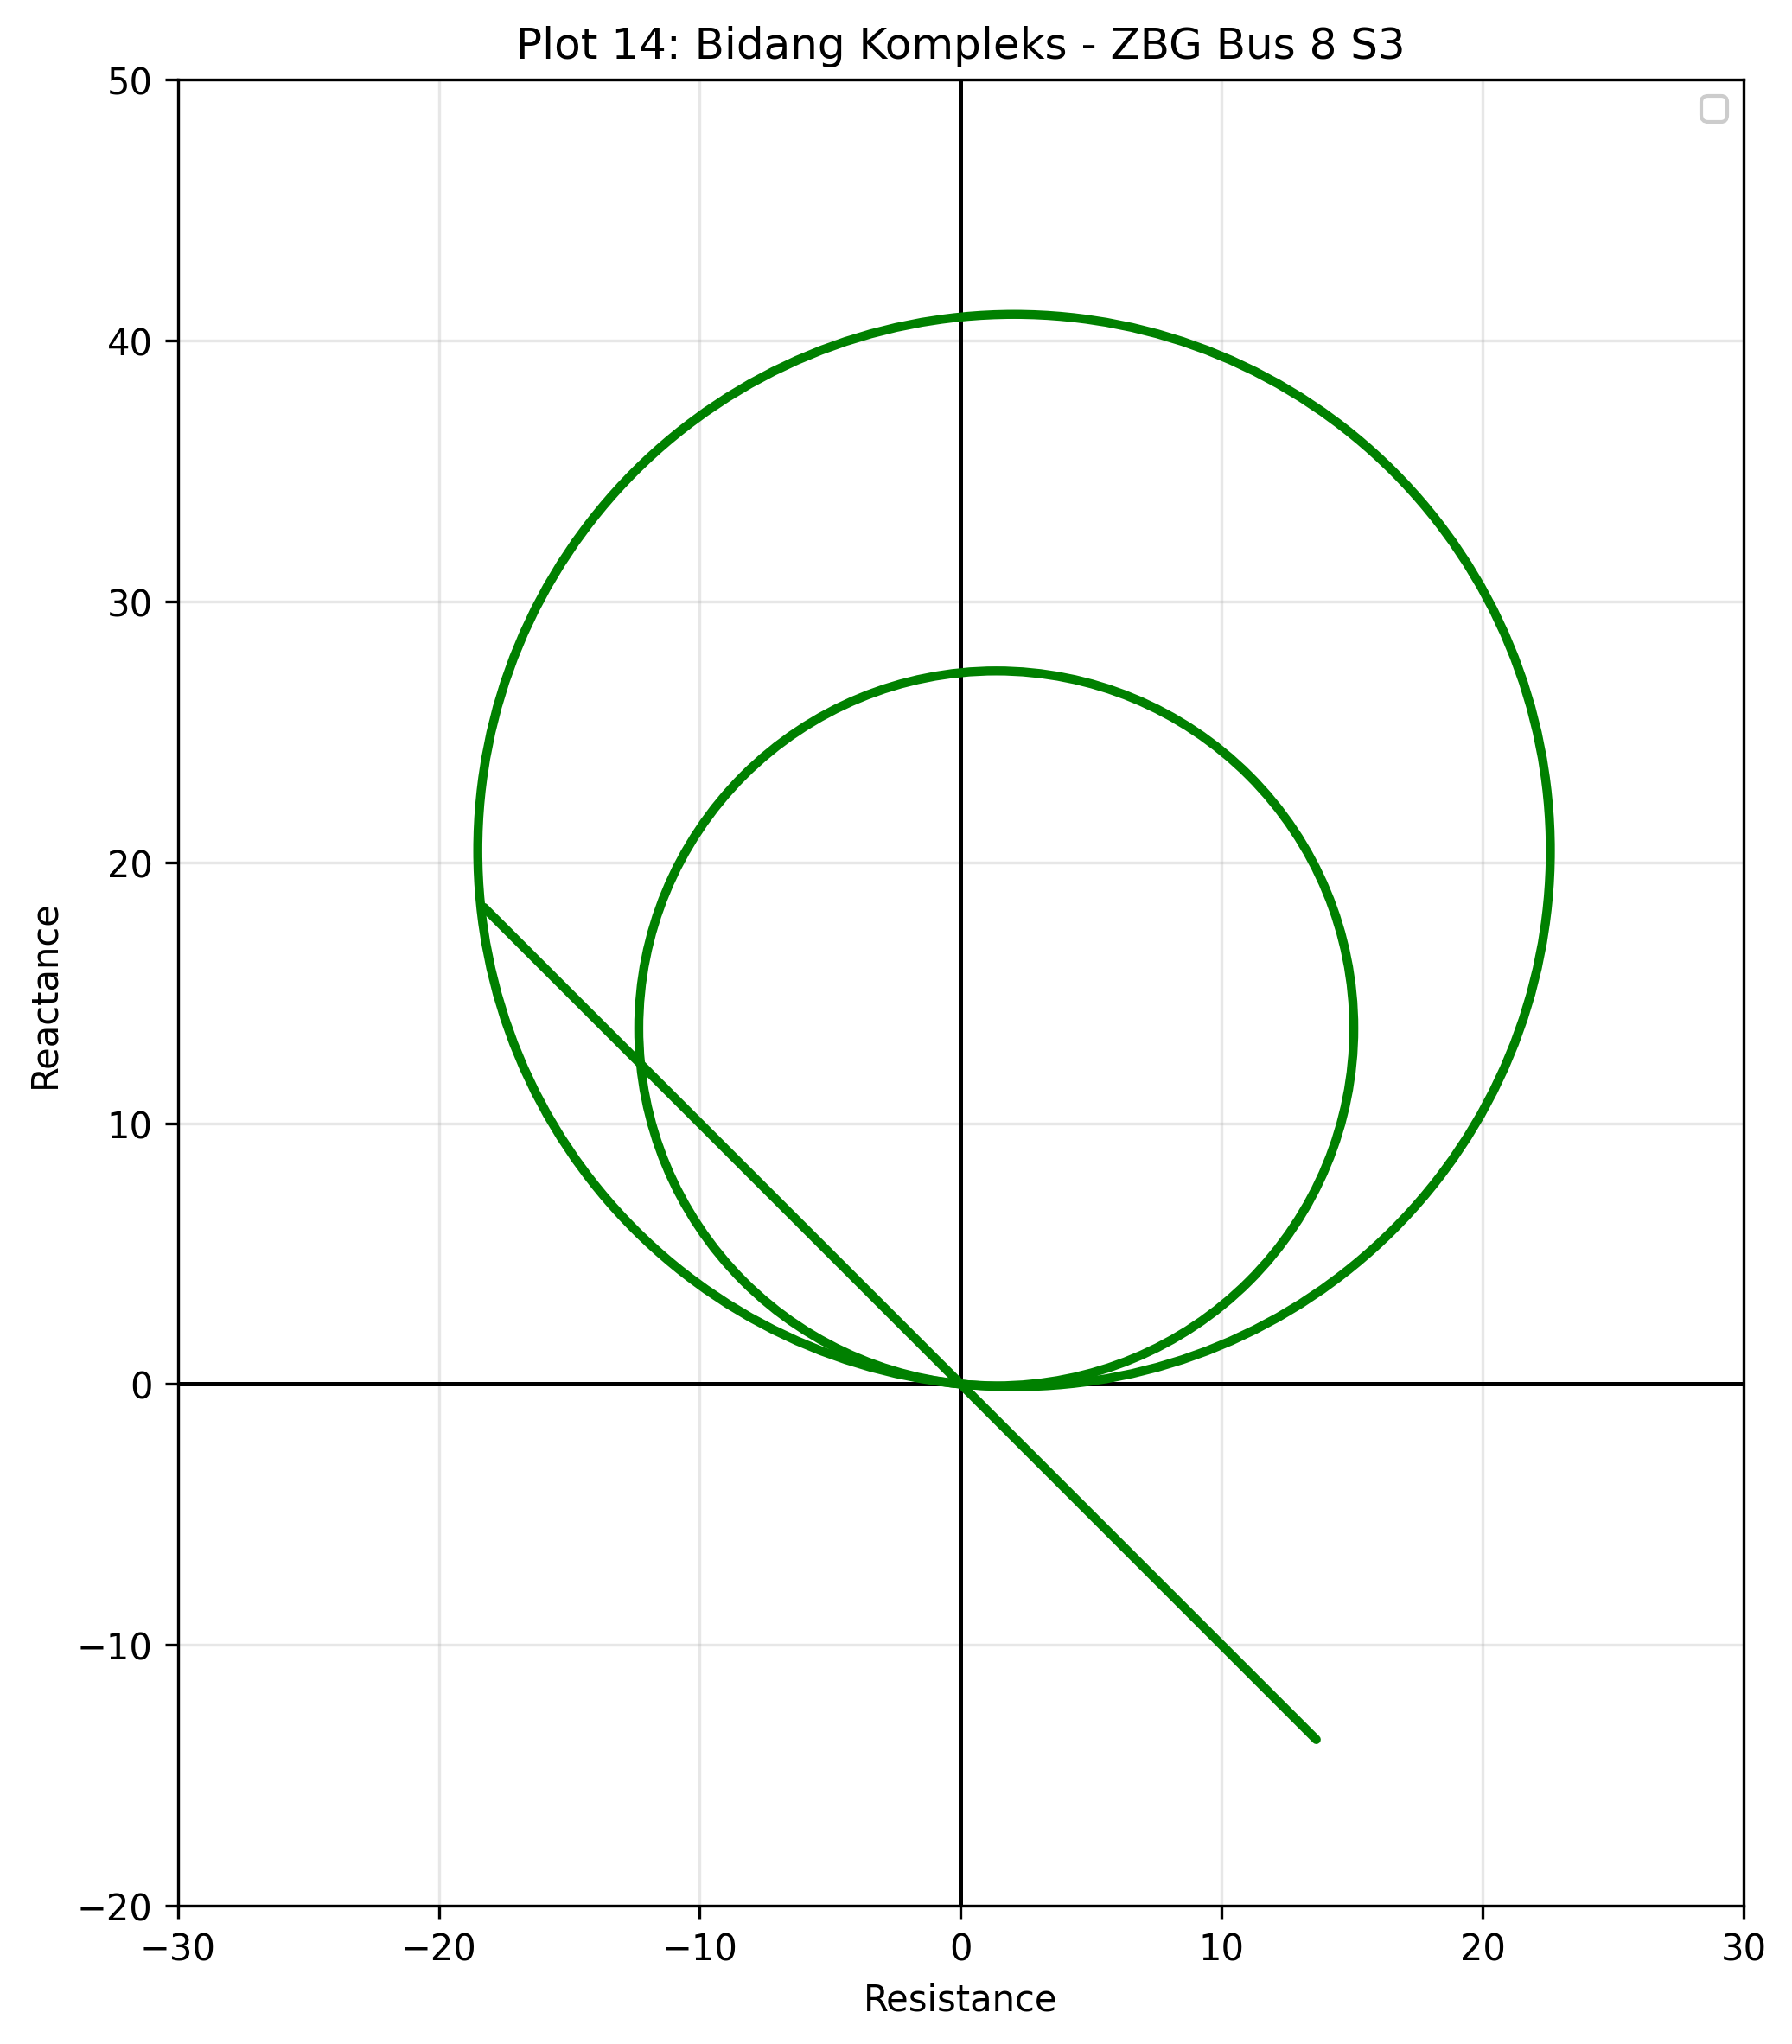
\includegraphics[width=\textwidth]{contents/chapter-4/PRIZI_14_ZBG_Bus_8_S3.png}
        \caption{Zoom In Pada Zona Proteksi}
        \label{fig:PRIZI_14_ZBG_Bus_8_S3}
    \end{subfigure}

    \caption{Impedansi Tampak ZBG Bus 8 Skenario 3}
    \label{fig:Impedansi_Tampak_ZBG_Bus_8_S3}
\end{figure}

Gambar \ref{fig:Impedansi_Tampak_ZBG_Bus_8_S3} menunjukkan bahwa impedansi tampak loop fasa B dengan ground yang dibaca oleh relay 21 sisi Bus 8 juga tidak masuk ke dalam zona proteksi. Hasil tersebut masih konsisten dengan kondisi arus pada Gambar \ref{fig:Bus_8_Ex_DLG_S3}, yaitu arus yang terbaca belum memenuhi arus minimum untuk membuat relay aktif. Oleh karena itu, jika dibandingkan dengan acuan gangguan eksternal DLG pada Subbab \ref{subsec:tanpa_IBR_ex_dlg}, respons relay 21 sisi Bus 8 pada elemen ini juga menunjukkan \textit{misoperation}.

%%%%%%%%%%%%%%%%%%%%%%%%%%%%%%%%%%%%%%%%%%%%%%%%%%%%%%%%%%%%%%%

% \begin{figure}[H]
%     \centering
%     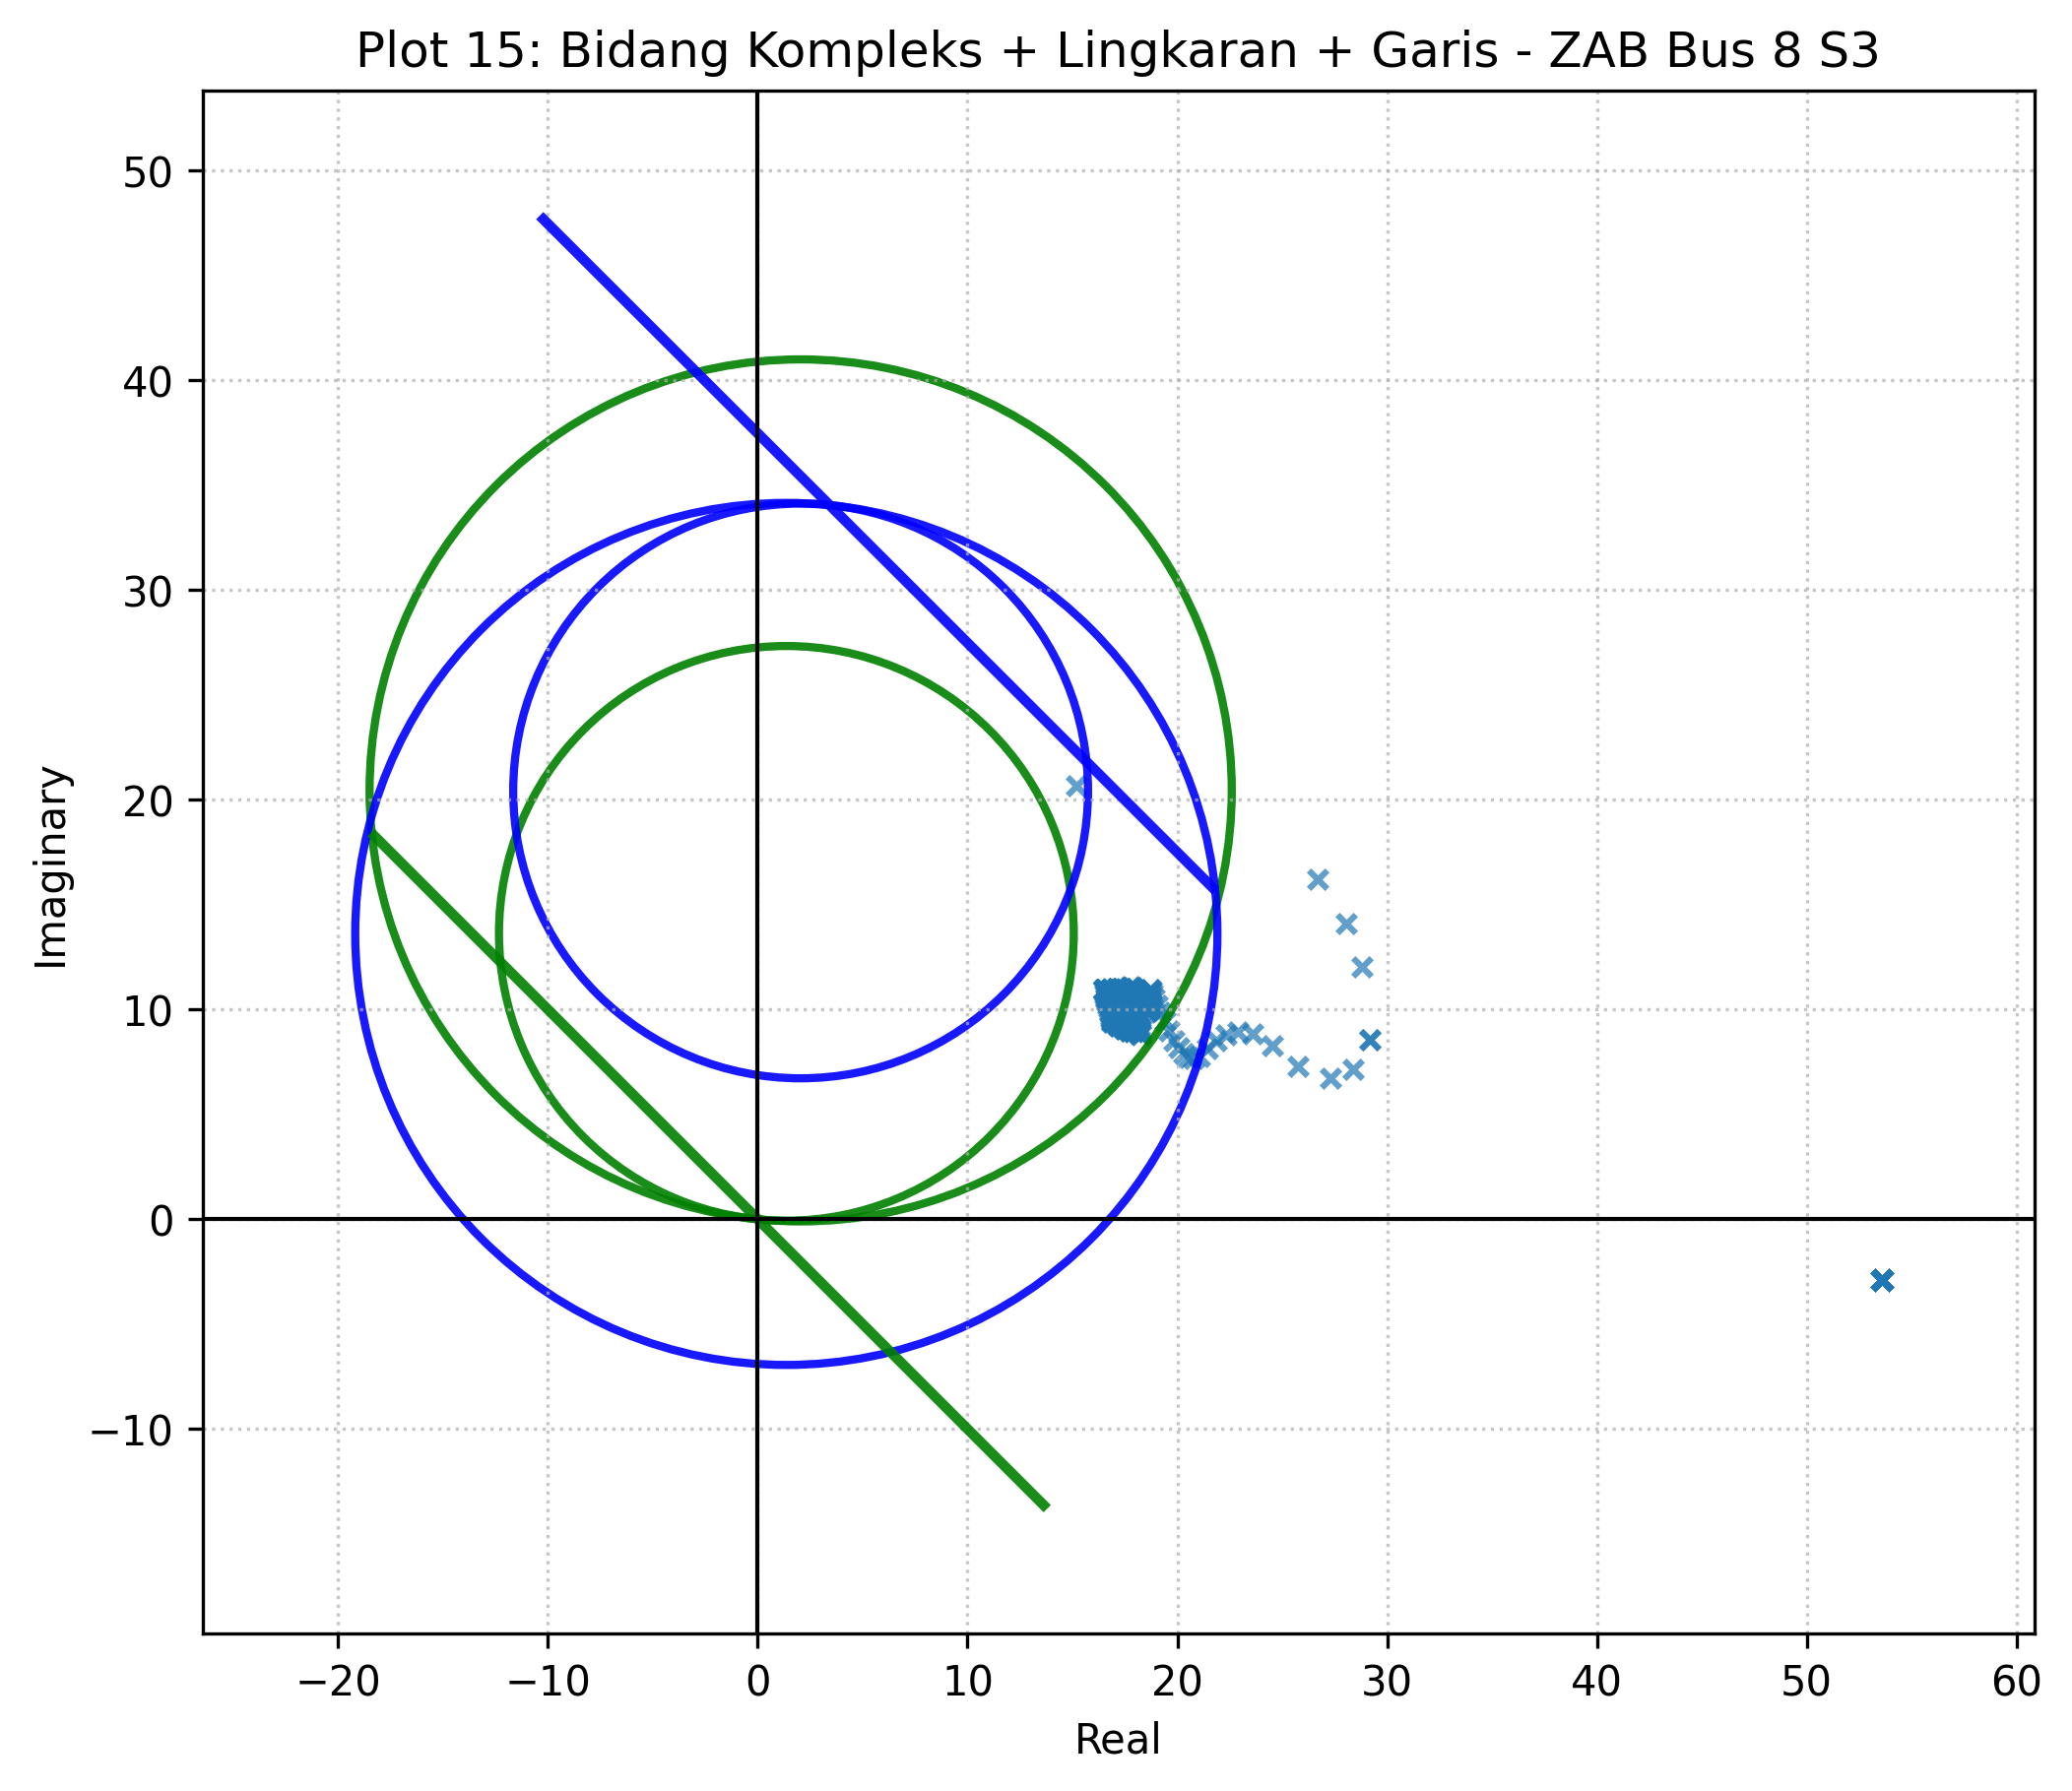
\includegraphics[width=0.8\textwidth]{contents/chapter-4/15_ZAB_Bus_8_S3_dengan_lingkaran_dan_garis.png}
%     \caption{Impedansi Tampak ZAB Bus 8 Skenario 3}
%     \label{fig:15_ZAB_Bus_8_S3_dengan_lingkaran_dan_garis}
% \end{figure}

% Terlihat pada gambar \ref{fig:15_ZAB_Bus_8_S3_dengan_lingkaran_dan_garis} bahwa impedansi tampak pada fasa A dengan fasa B yang dibaca oleh relay 21 sisi bus 8 saat terdapat gangguan mengalami over reach pada zona 1 serta mengalami drop out pada zona 2 sehingga dengan acuan pada \ref{subsec:tanpa_IBR_ex_dlg} relay 21 bus 8 mengalami missoperation trip pada zona 1.

%%%%%%%%%%%%%%%%%%%%%%%%%%%%%%%%%SISI PRIMER%%%%%%%%%%%%%%%%%%%%%%%%%%%%%%%%%%

% \begin{figure}[H]
%     \centering
%     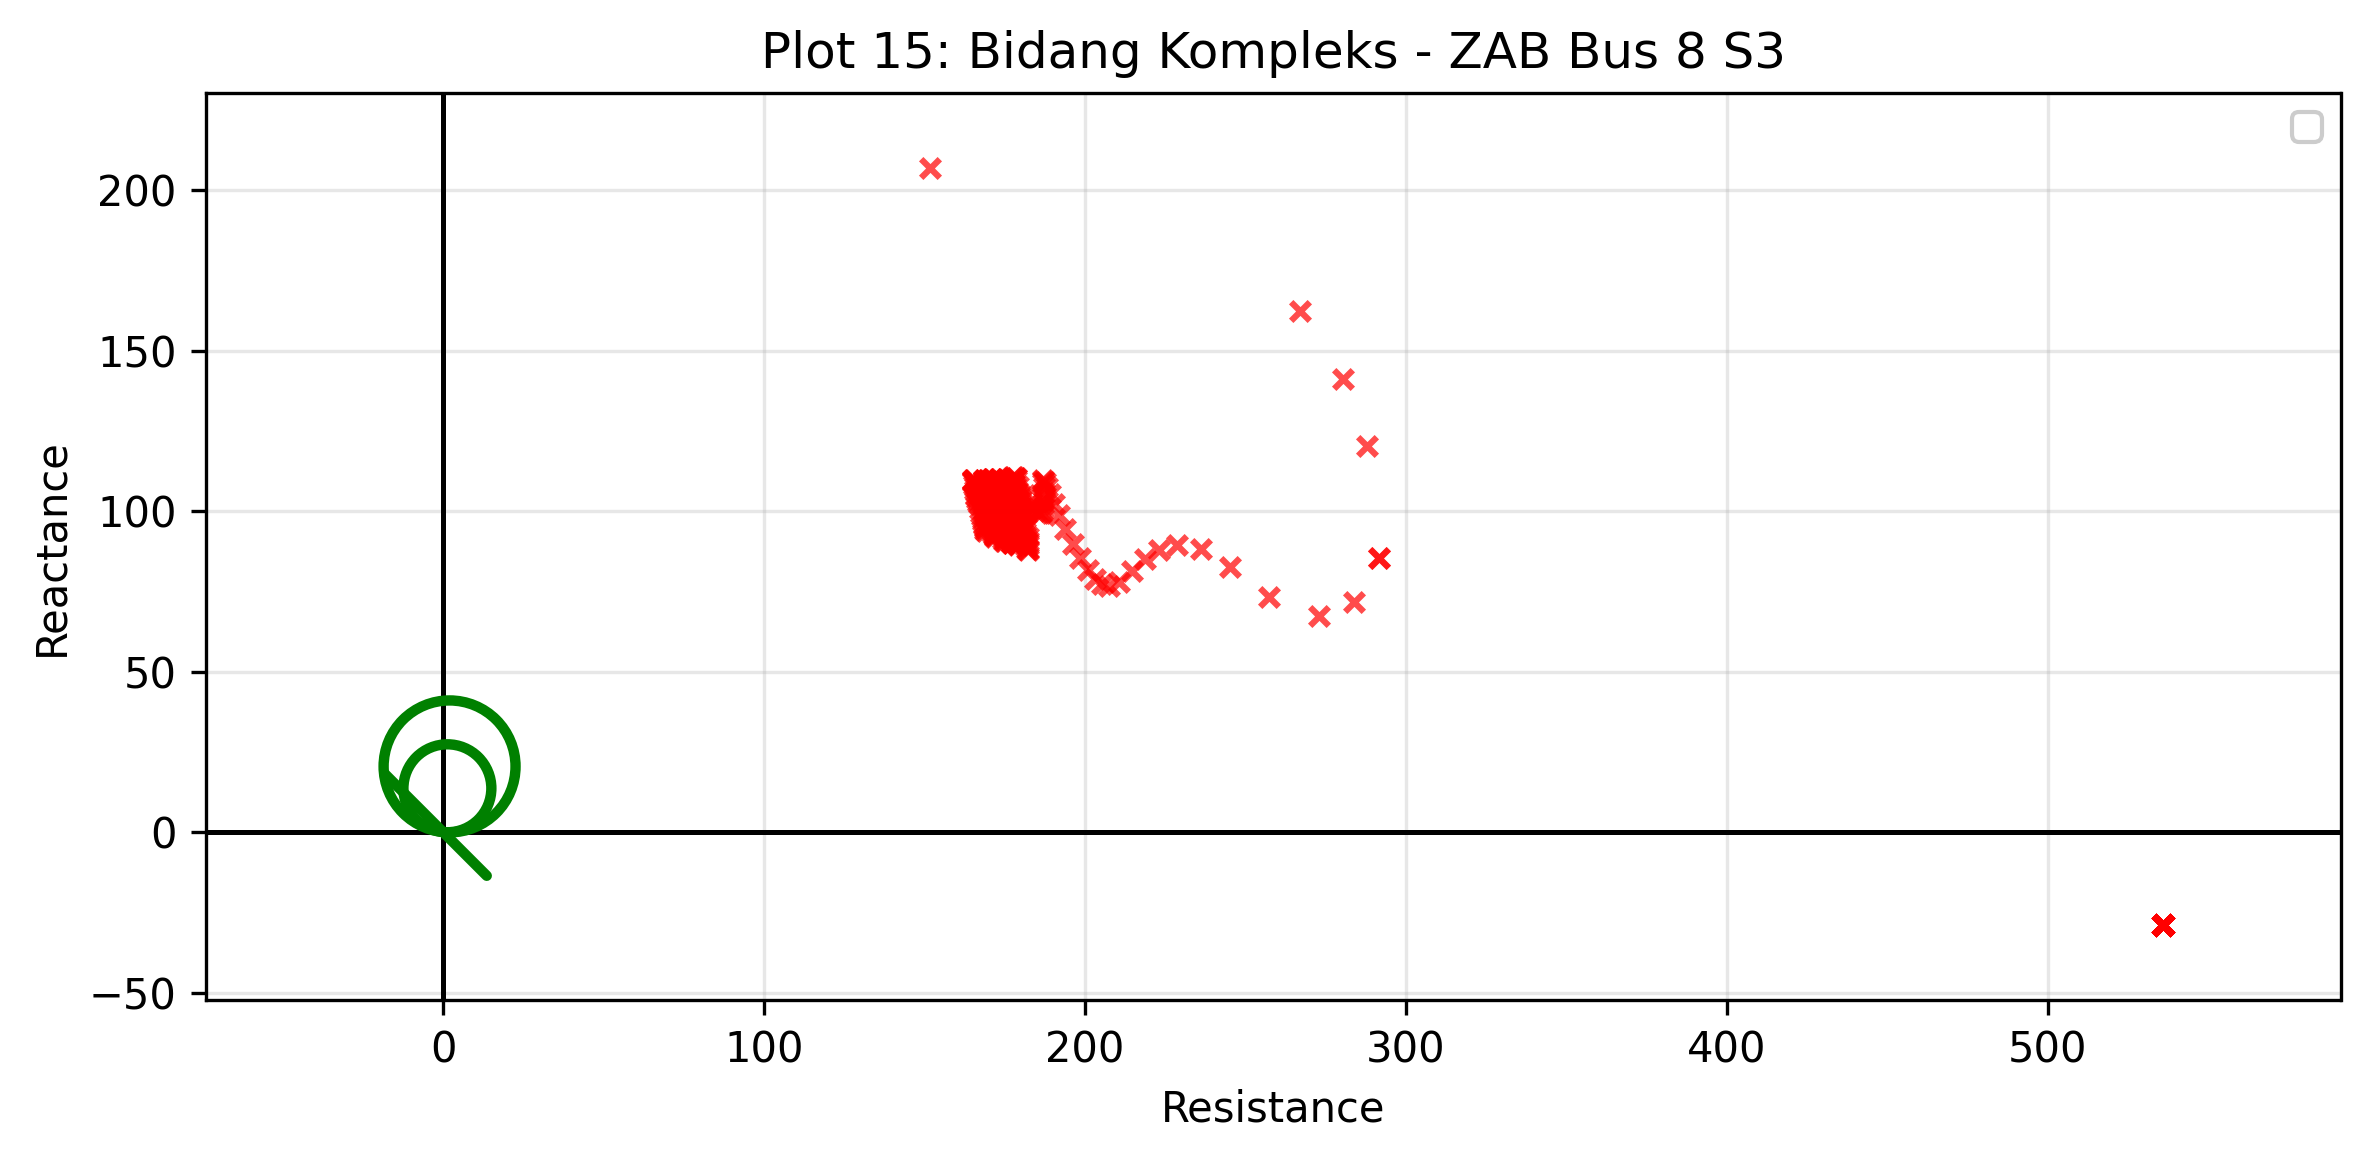
\includegraphics[width=0.8\textwidth]{contents/chapter-4/PRIA_15_ZAB_Bus_8_S3.png}
%     \caption{Impedansi Tampak ZAB Bus 8 Skenario 3}
%     \label{fig:PRIA_15_ZAB_Bus_8_S3}
% \end{figure}

% \begin{figure}[H]
%     \centering
%     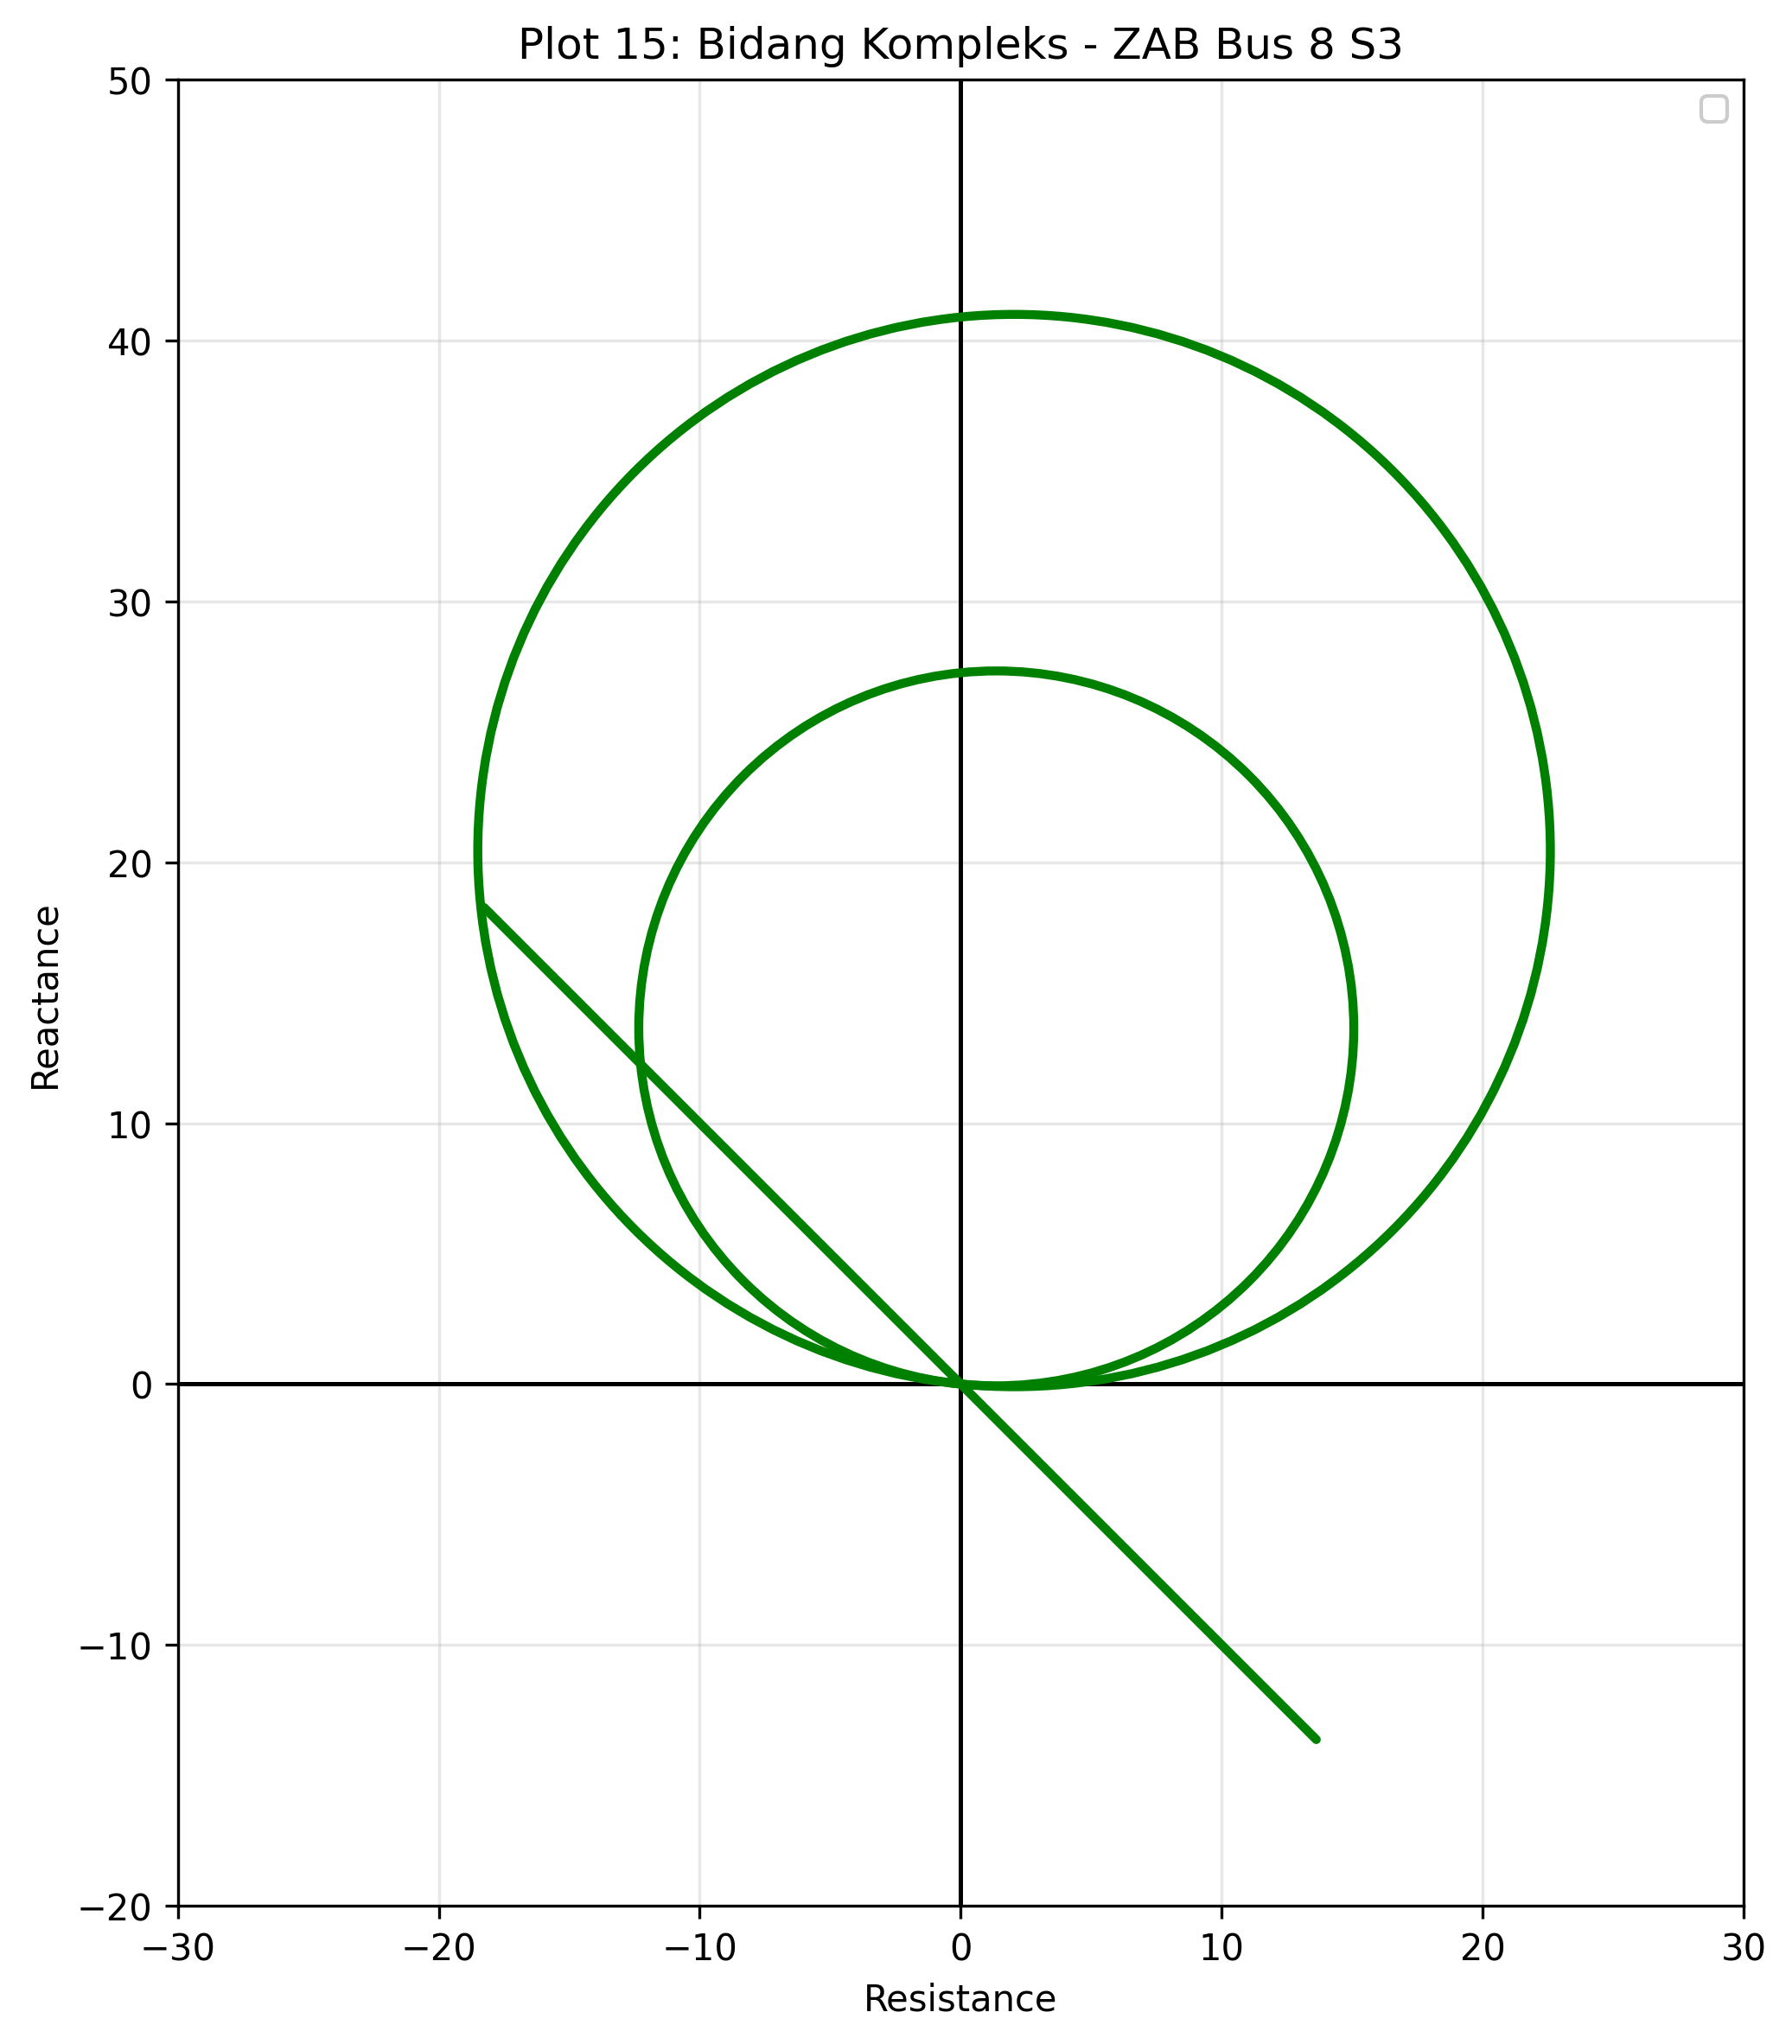
\includegraphics[width=0.8\textwidth]{contents/chapter-4/PRIZI_15_ZAB_Bus_8_S3.png}
%     \caption{Impedansi Tampak ZAB Bus 8 Skenario 3}
%     \label{fig:PRIZI_15_ZAB_Bus_8_S3}
% \end{figure}

\begin{figure}[H]
    \centering

    % Gambar sebelah kiri
    \begin{subfigure}[t]{0.48\textwidth}
        \centering
        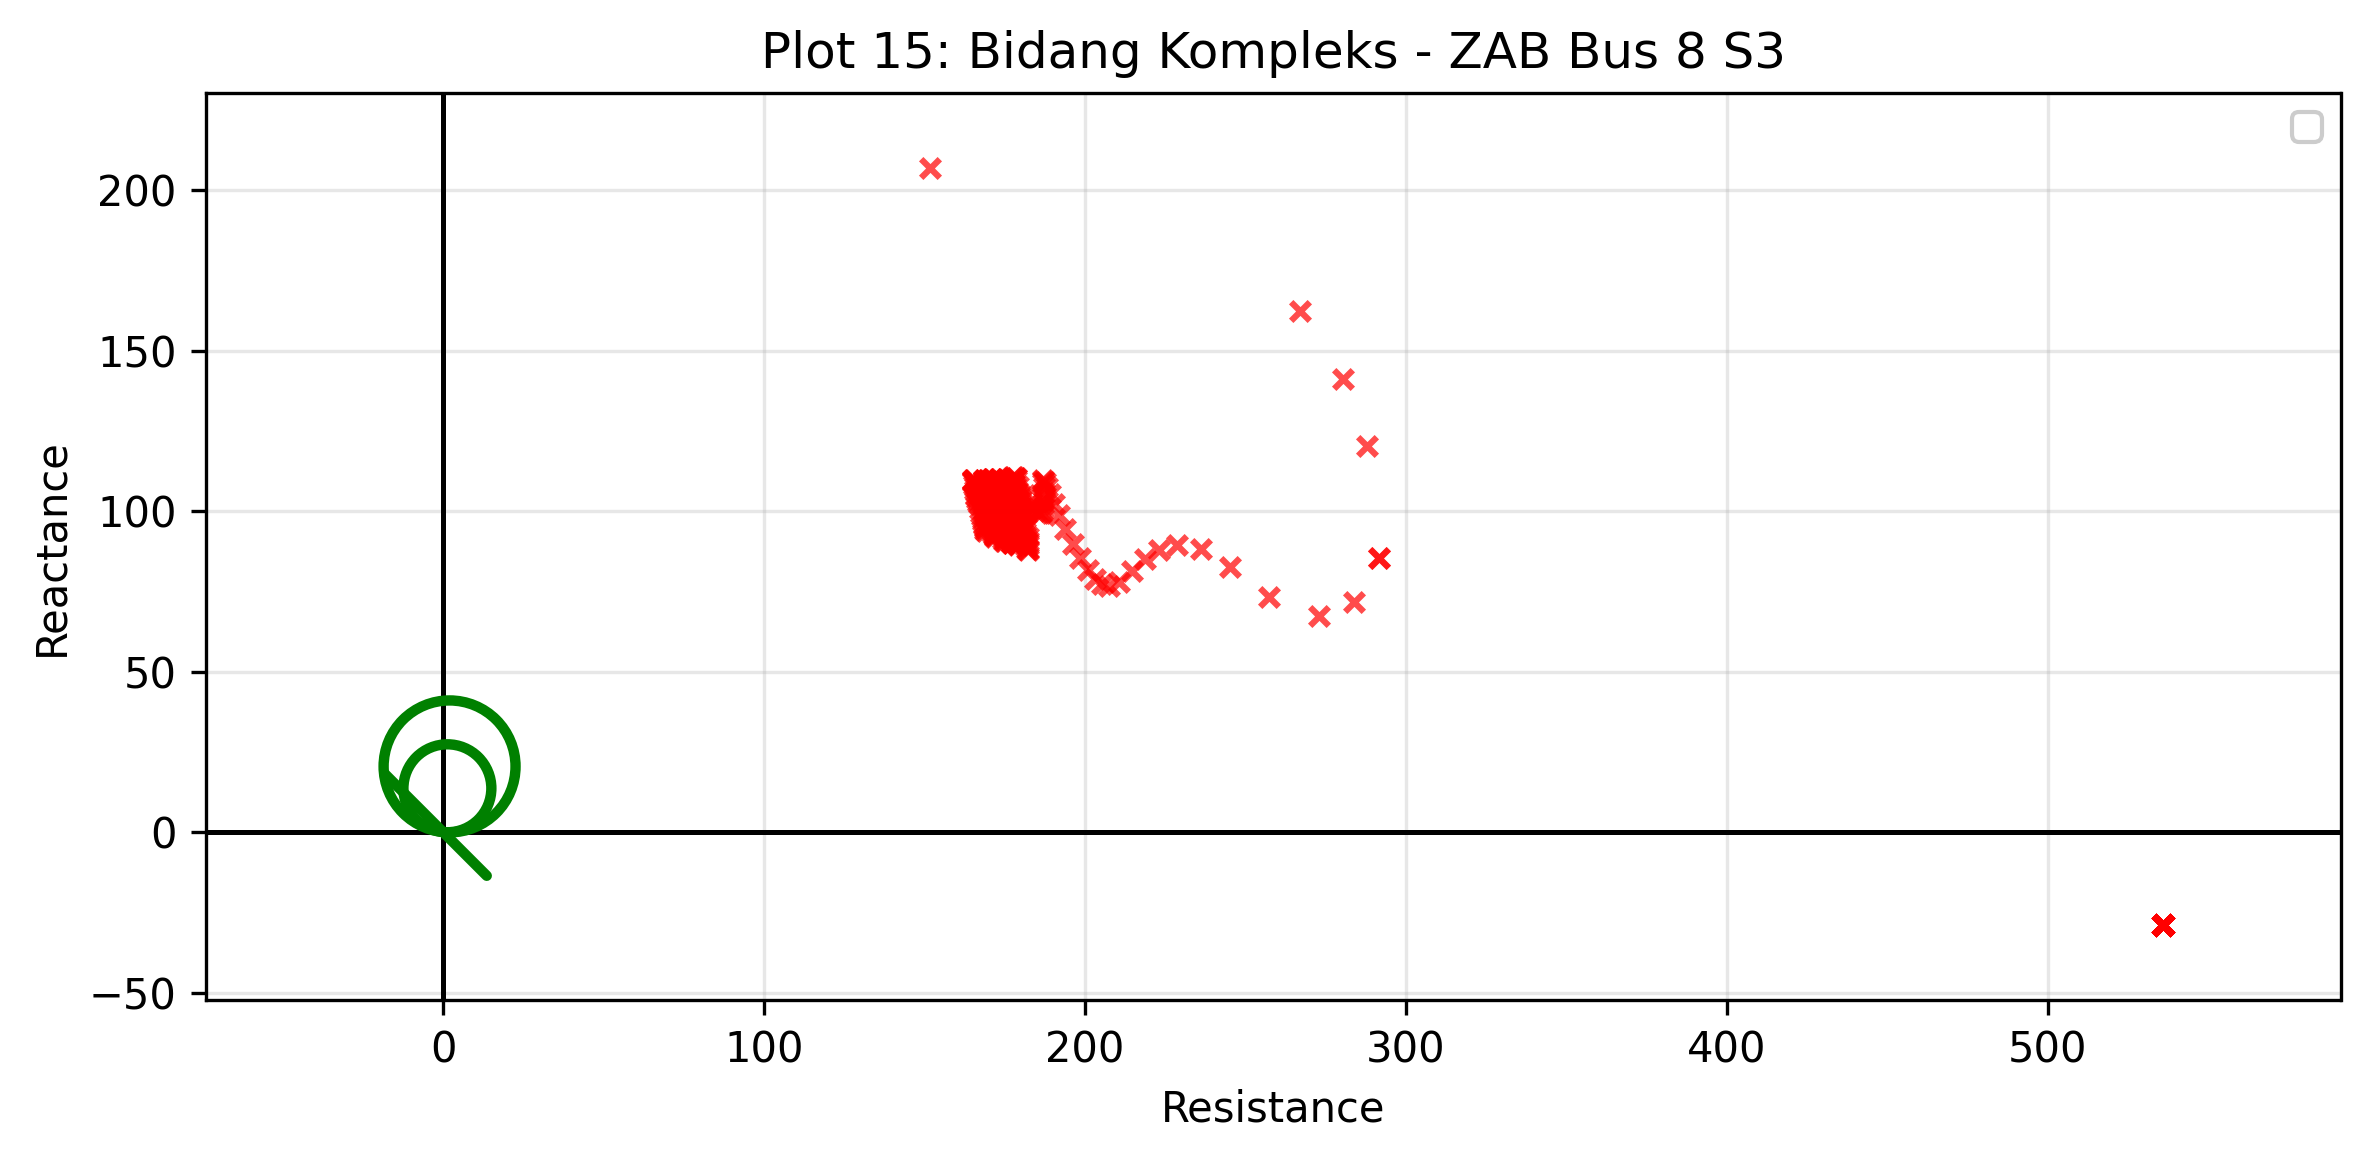
\includegraphics[width=\textwidth]{contents/chapter-4/PRIA_15_ZAB_Bus_8_S3.png}
        \caption{Seluruh Impedansi Tampak}
        \label{fig:PRIA_15_ZAB_Bus_8_S3}
    \end{subfigure}
    \hfill
    % Gambar sebelah kanan
    \begin{subfigure}[t]{0.48\textwidth}
        \centering
        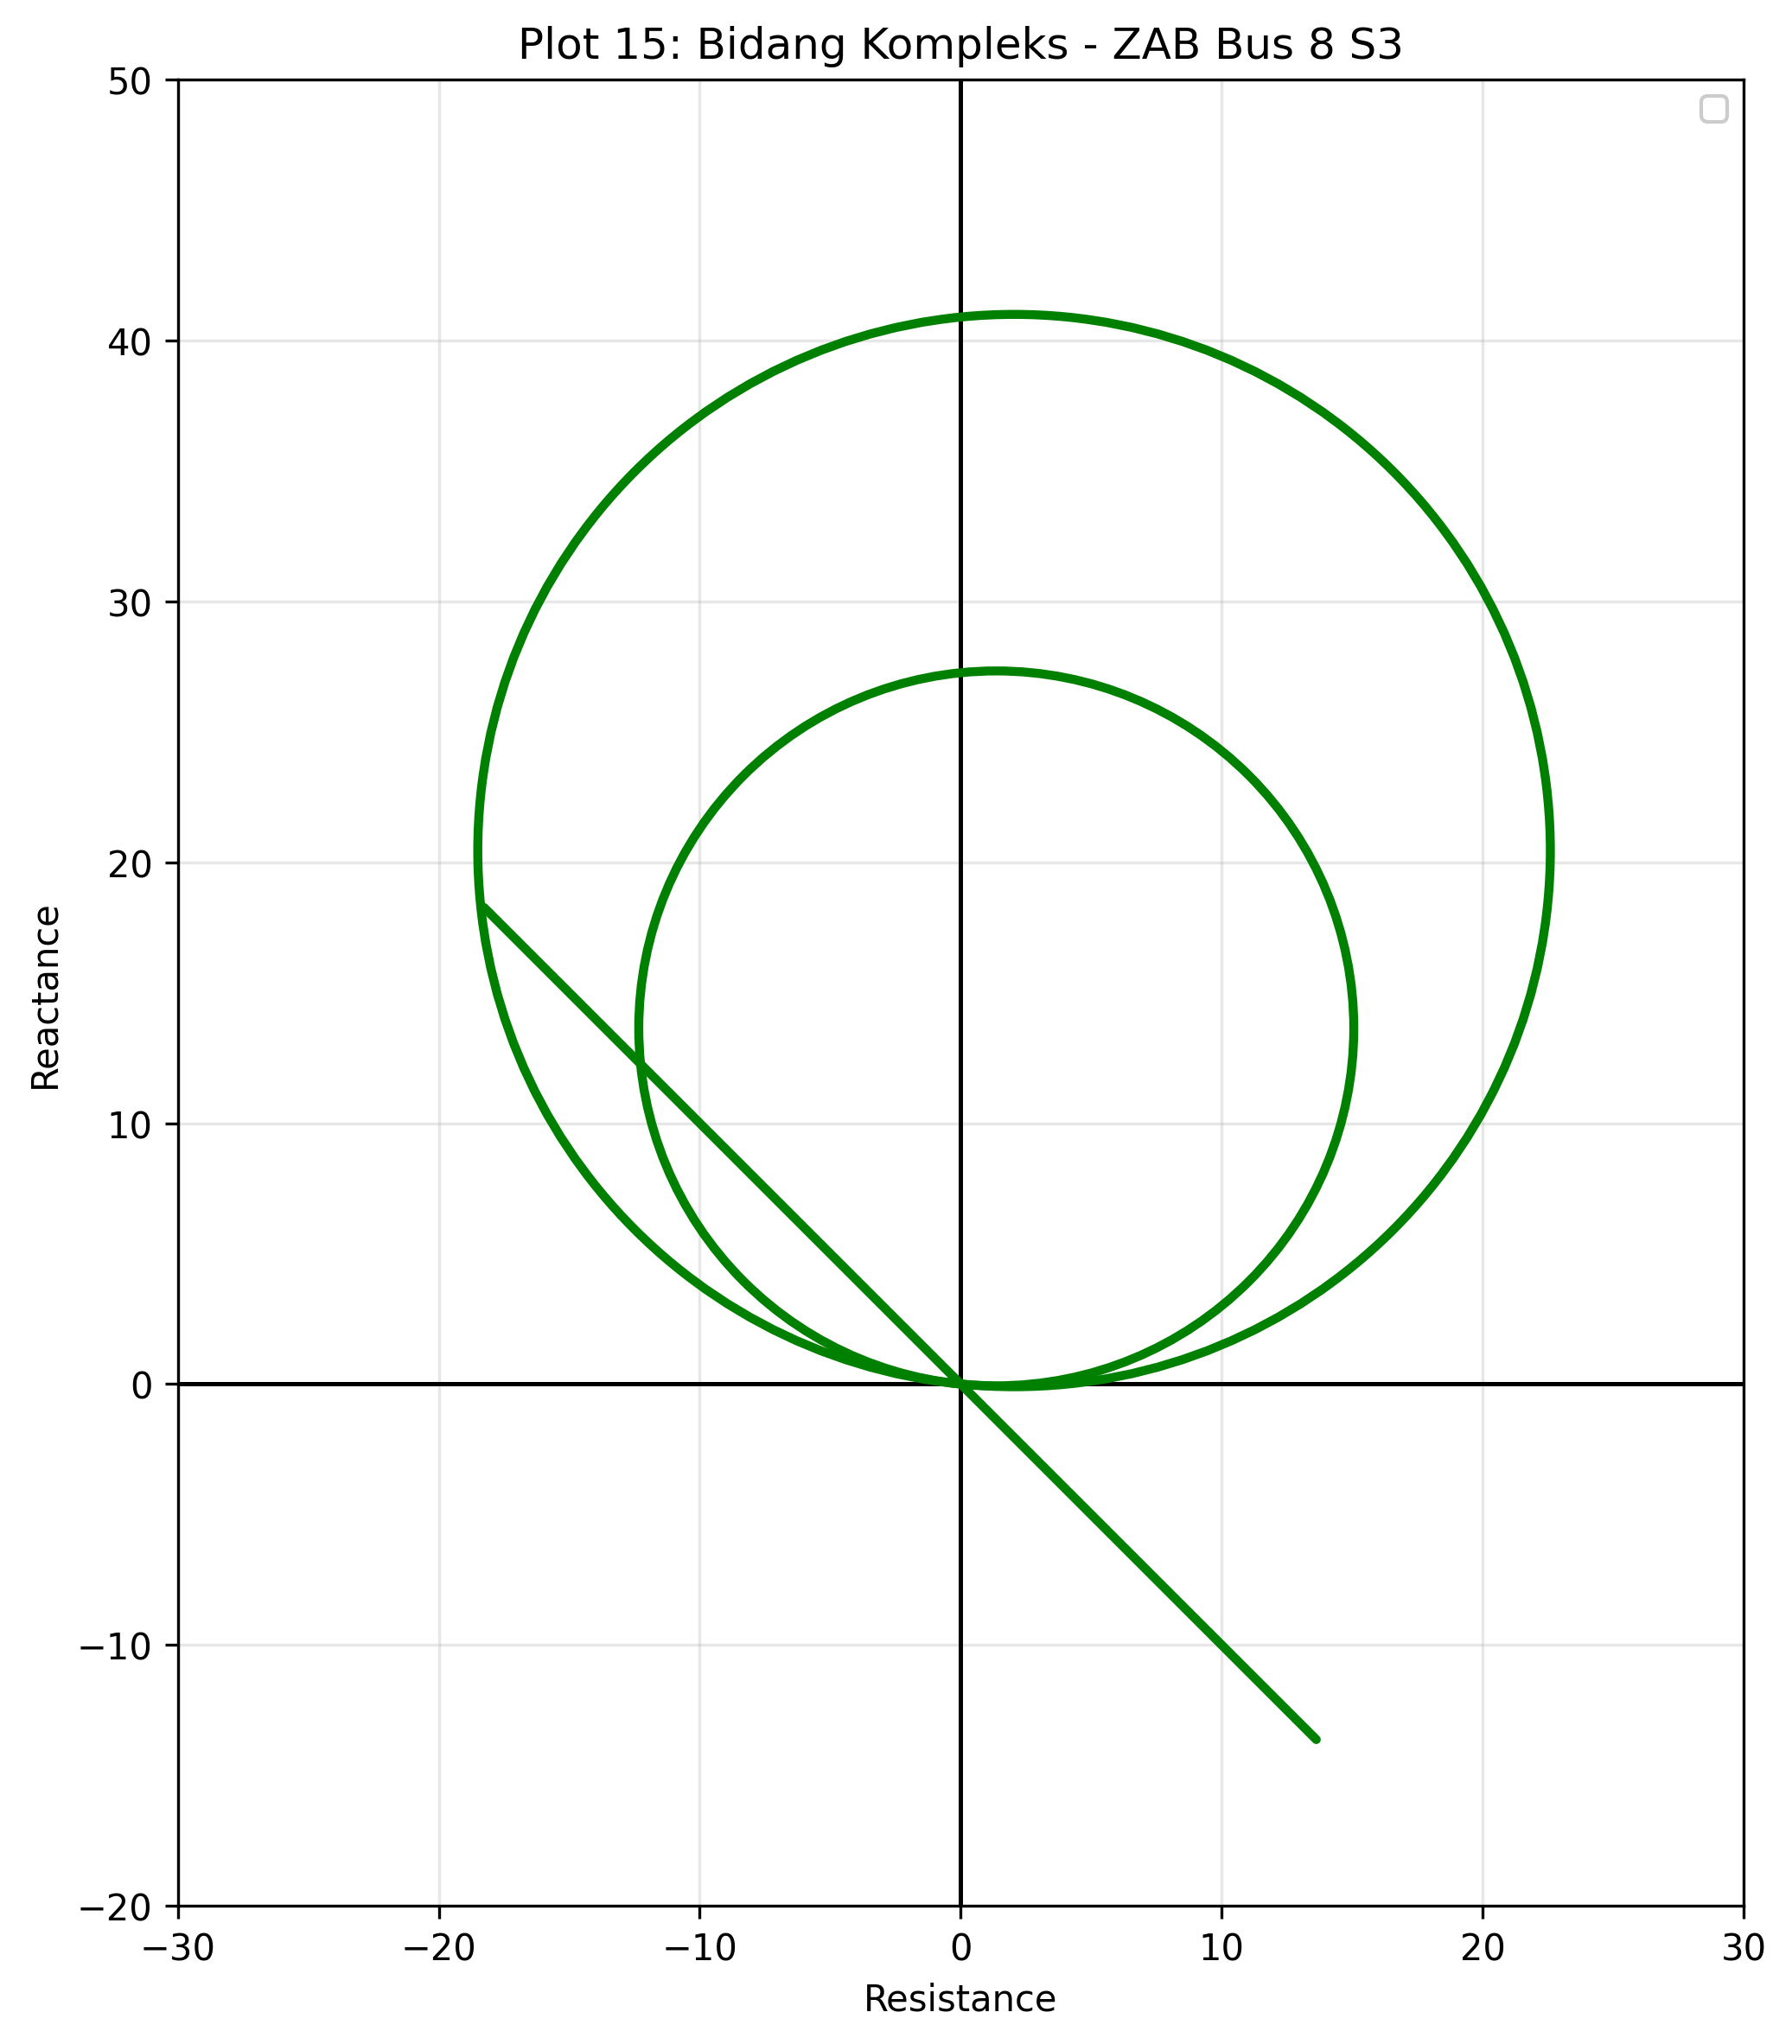
\includegraphics[width=\textwidth]{contents/chapter-4/PRIZI_15_ZAB_Bus_8_S3.png}
        \caption{Zoom In Pada Zona Proteksi}
        \label{fig:PRIZI_15_ZAB_Bus_8_S3}
    \end{subfigure}

    \caption{Impedansi Tampak ZAB Bus 8 Skenario 3}
    \label{fig:Impedansi_Tampak_ZAB_Bus_8_S3}
\end{figure}

Gambar \ref{fig:Impedansi_Tampak_ZAB_Bus_8_S3} menunjukkan bahwa impedansi tampak loop fasa A dengan fasa B yang dibaca oleh relay 21 sisi Bus 8 tidak masuk ke dalam zona proteksi. Sama seperti dua elemen sebelumnya, kondisi ini berkaitan dengan arus sekunder CT pada Gambar \ref{fig:Bus_8_Ex_DLG_S3} yang belum memenuhi arus minimum untuk membuat relay aktif. Dengan demikian, berdasarkan acuan gangguan eksternal DLG pada Subbab \ref{subsec:tanpa_IBR_ex_dlg}, respons relay 21 sisi Bus 8 pada skenario 3 menunjukkan \textit{misoperation}.

%%%%%%%%%%%%%%%%%%%%%%%%%%%%%%%%%%%%%%%%%%%%%%%%%%%%%%%%%%%%%%%

% \begin{figure}[H]
%     \centering
%     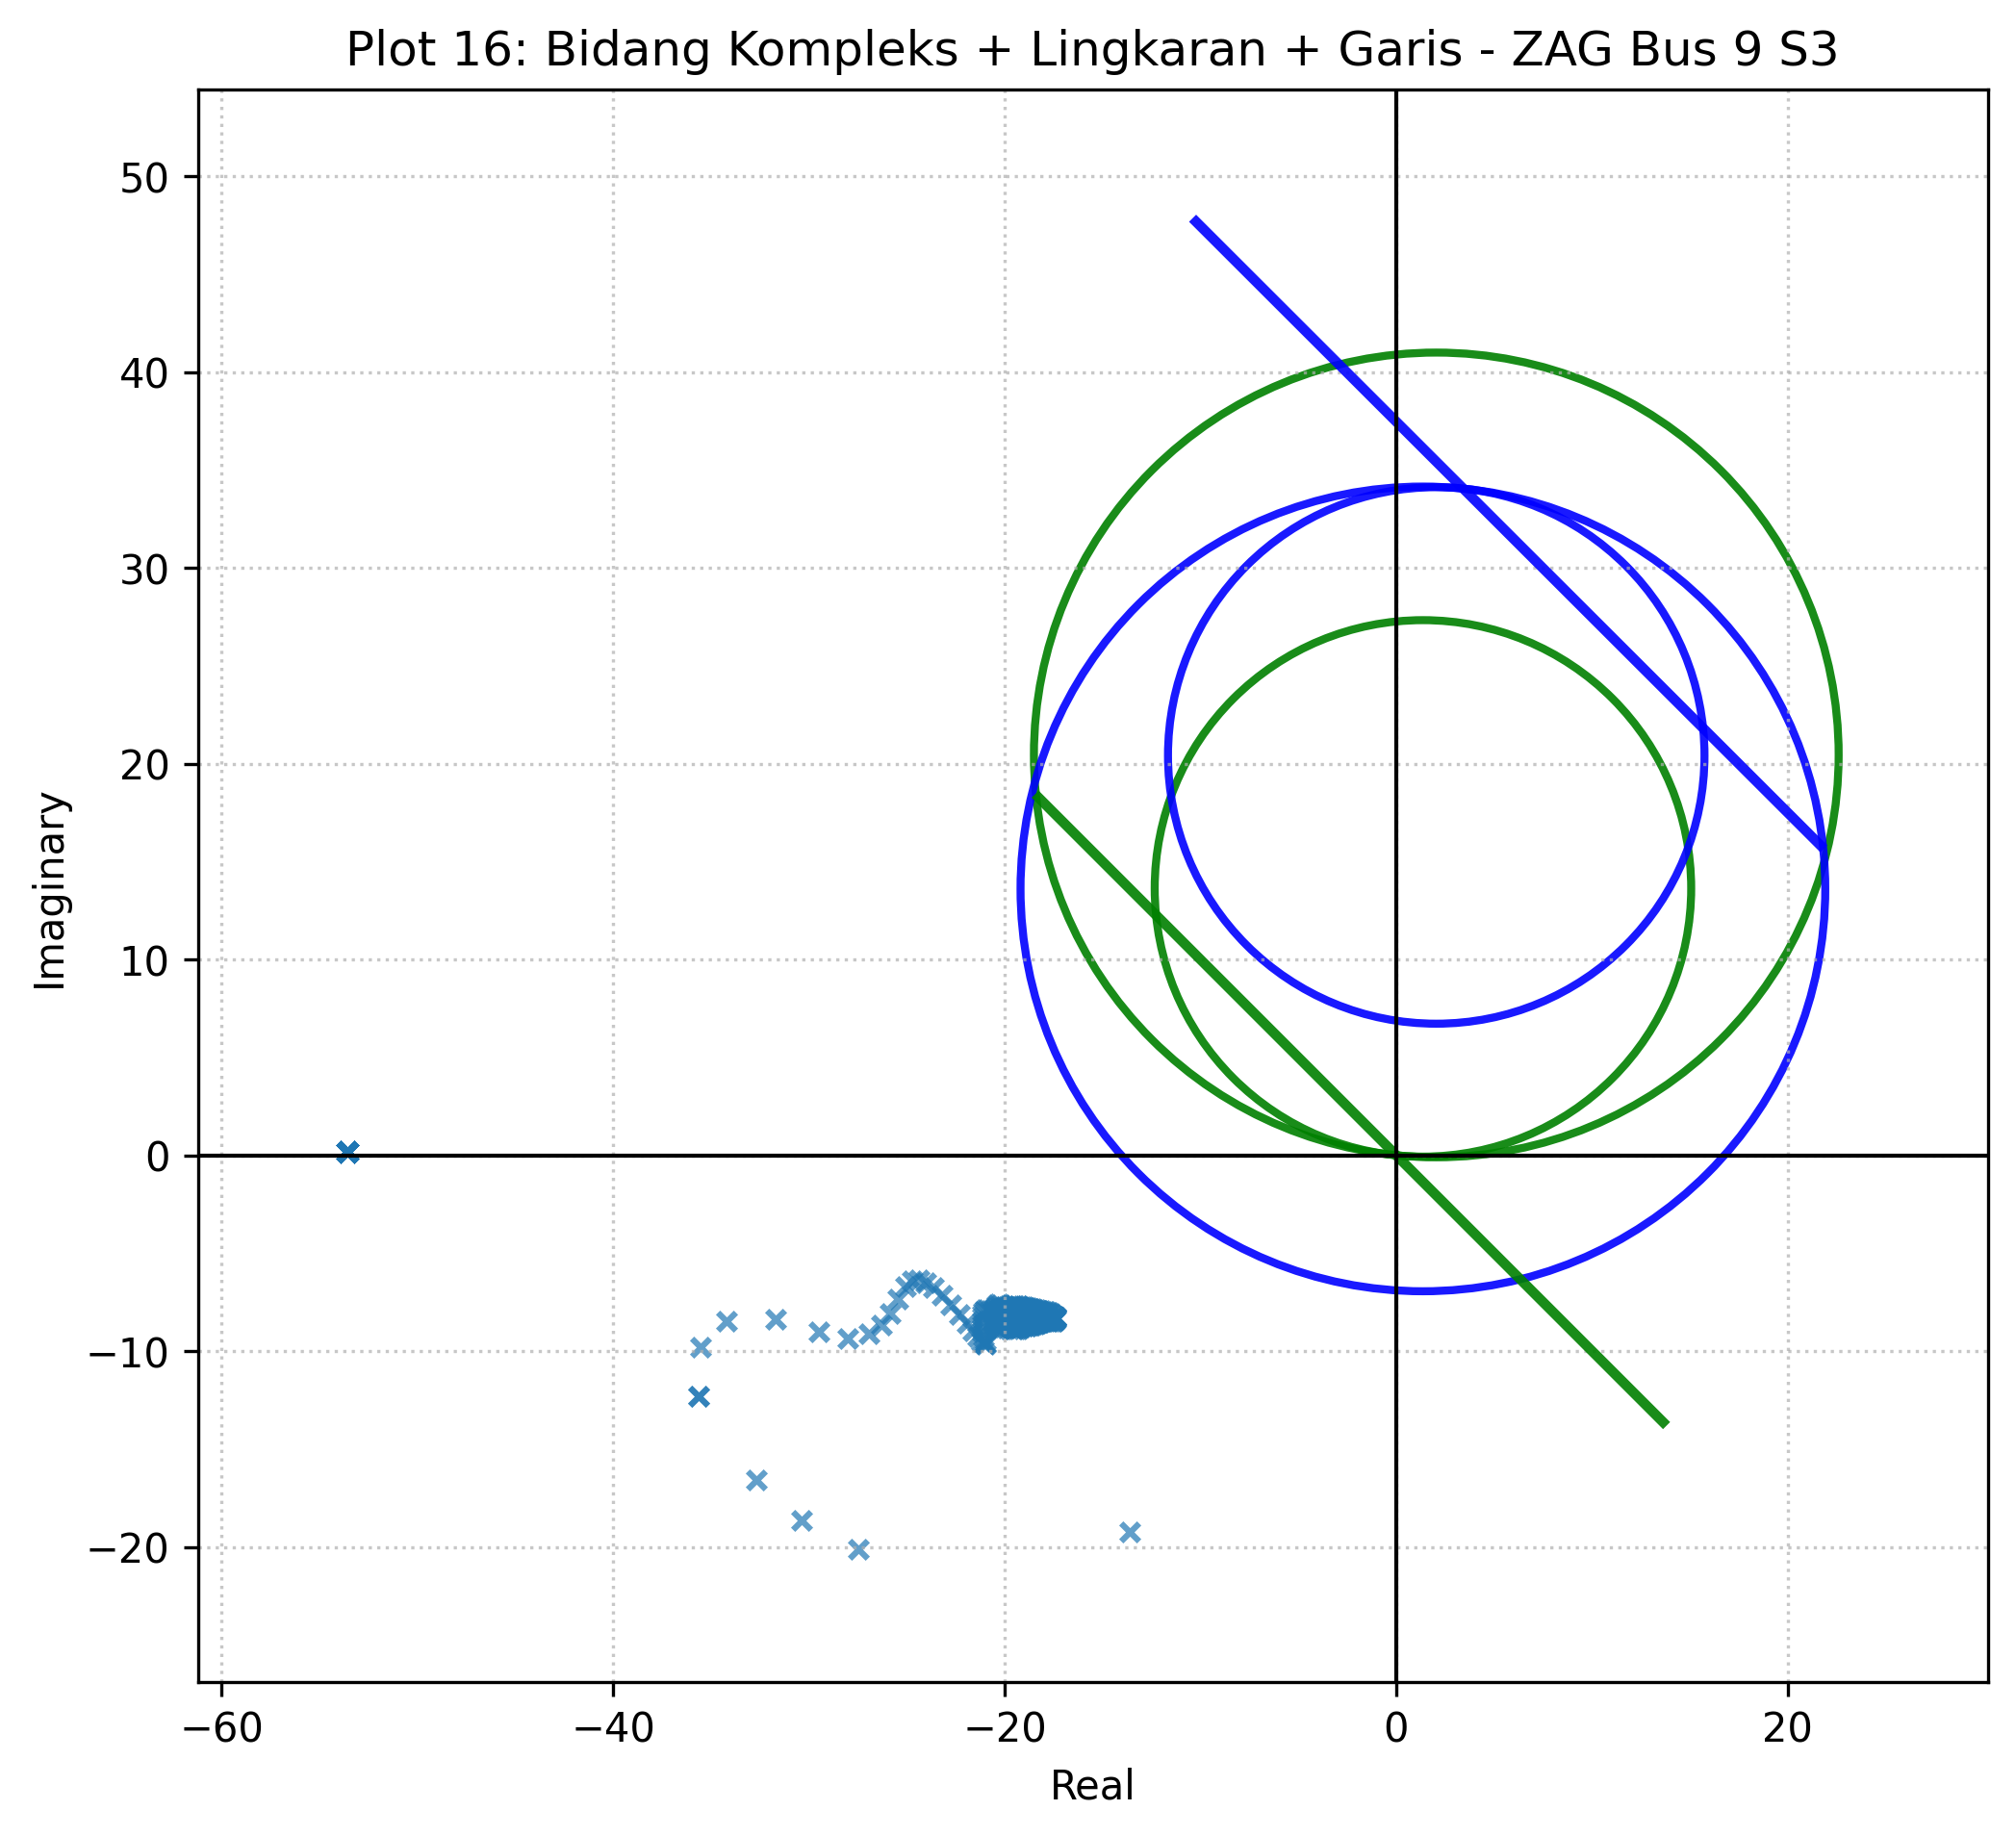
\includegraphics[width=0.8\textwidth]{contents/chapter-4/16_ZAG_Bus_9_S3_dengan_lingkaran_dan_garis.png}
%     \caption{Impedansi Tampak ZAG Bus 9 Skenario 3}
%     \label{fig:16_ZAG_Bus_9_S3_dengan_lingkaran_dan_garis}
% \end{figure} 

% Terlihat pada gambar \ref{fig:16_ZAG_Bus_9_S3_dengan_lingkaran_dan_garis} bahwa impedansi tampak pada fasa A dengan ground yang dibaca oleh relay 21 sisi bus 9 saat terdapat gangguan bekerja dengan baik sesuai acuan pada \ref{subsec:tanpa_IBR_ex_dlg} relay 21 bus 9 tidak mendeteksi adanya gangguan sehingga tidak mengirimkan sinyal trip kepada CB.

%%%%%%%%%%%%%%%%%%%%%%%%%%%%%%%%%SISI PRIMER%%%%%%%%%%%%%%%%%%%%%%%%%%%%%%%%%%

% \begin{figure}[H]
%     \centering
%     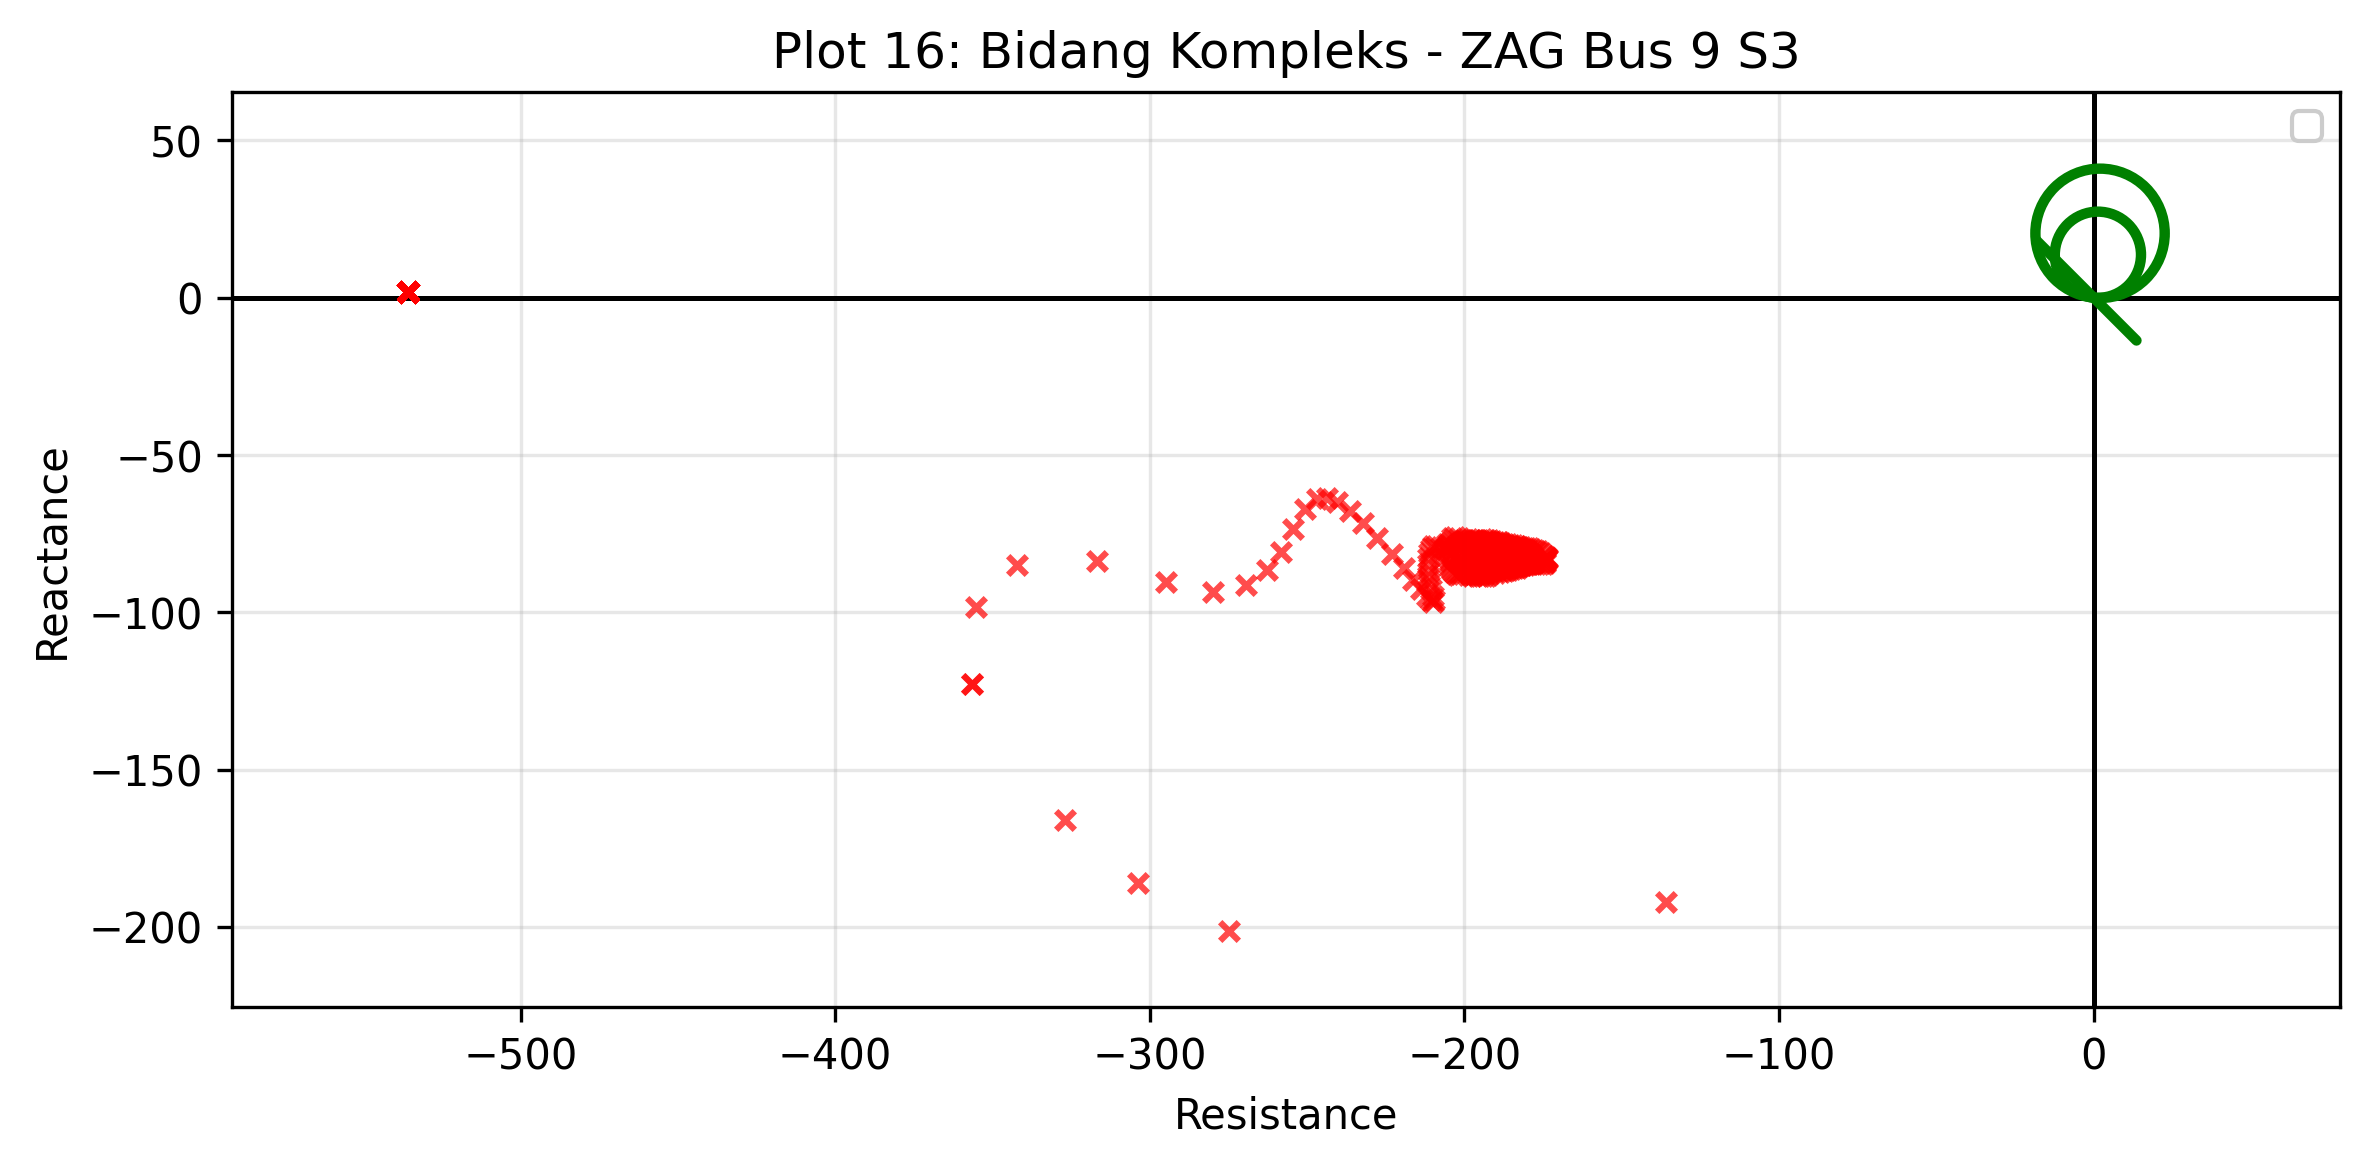
\includegraphics[width=0.8\textwidth]{contents/chapter-4/PRIA_16_ZAG_Bus_9_S3.png}
%     \caption{Impedansi Tampak ZAG Bus 9 Skenario 3}
%     \label{fig:PRIA_16_ZAG_Bus_9_S3}
% \end{figure}

% \begin{figure}[H]
%     \centering
%     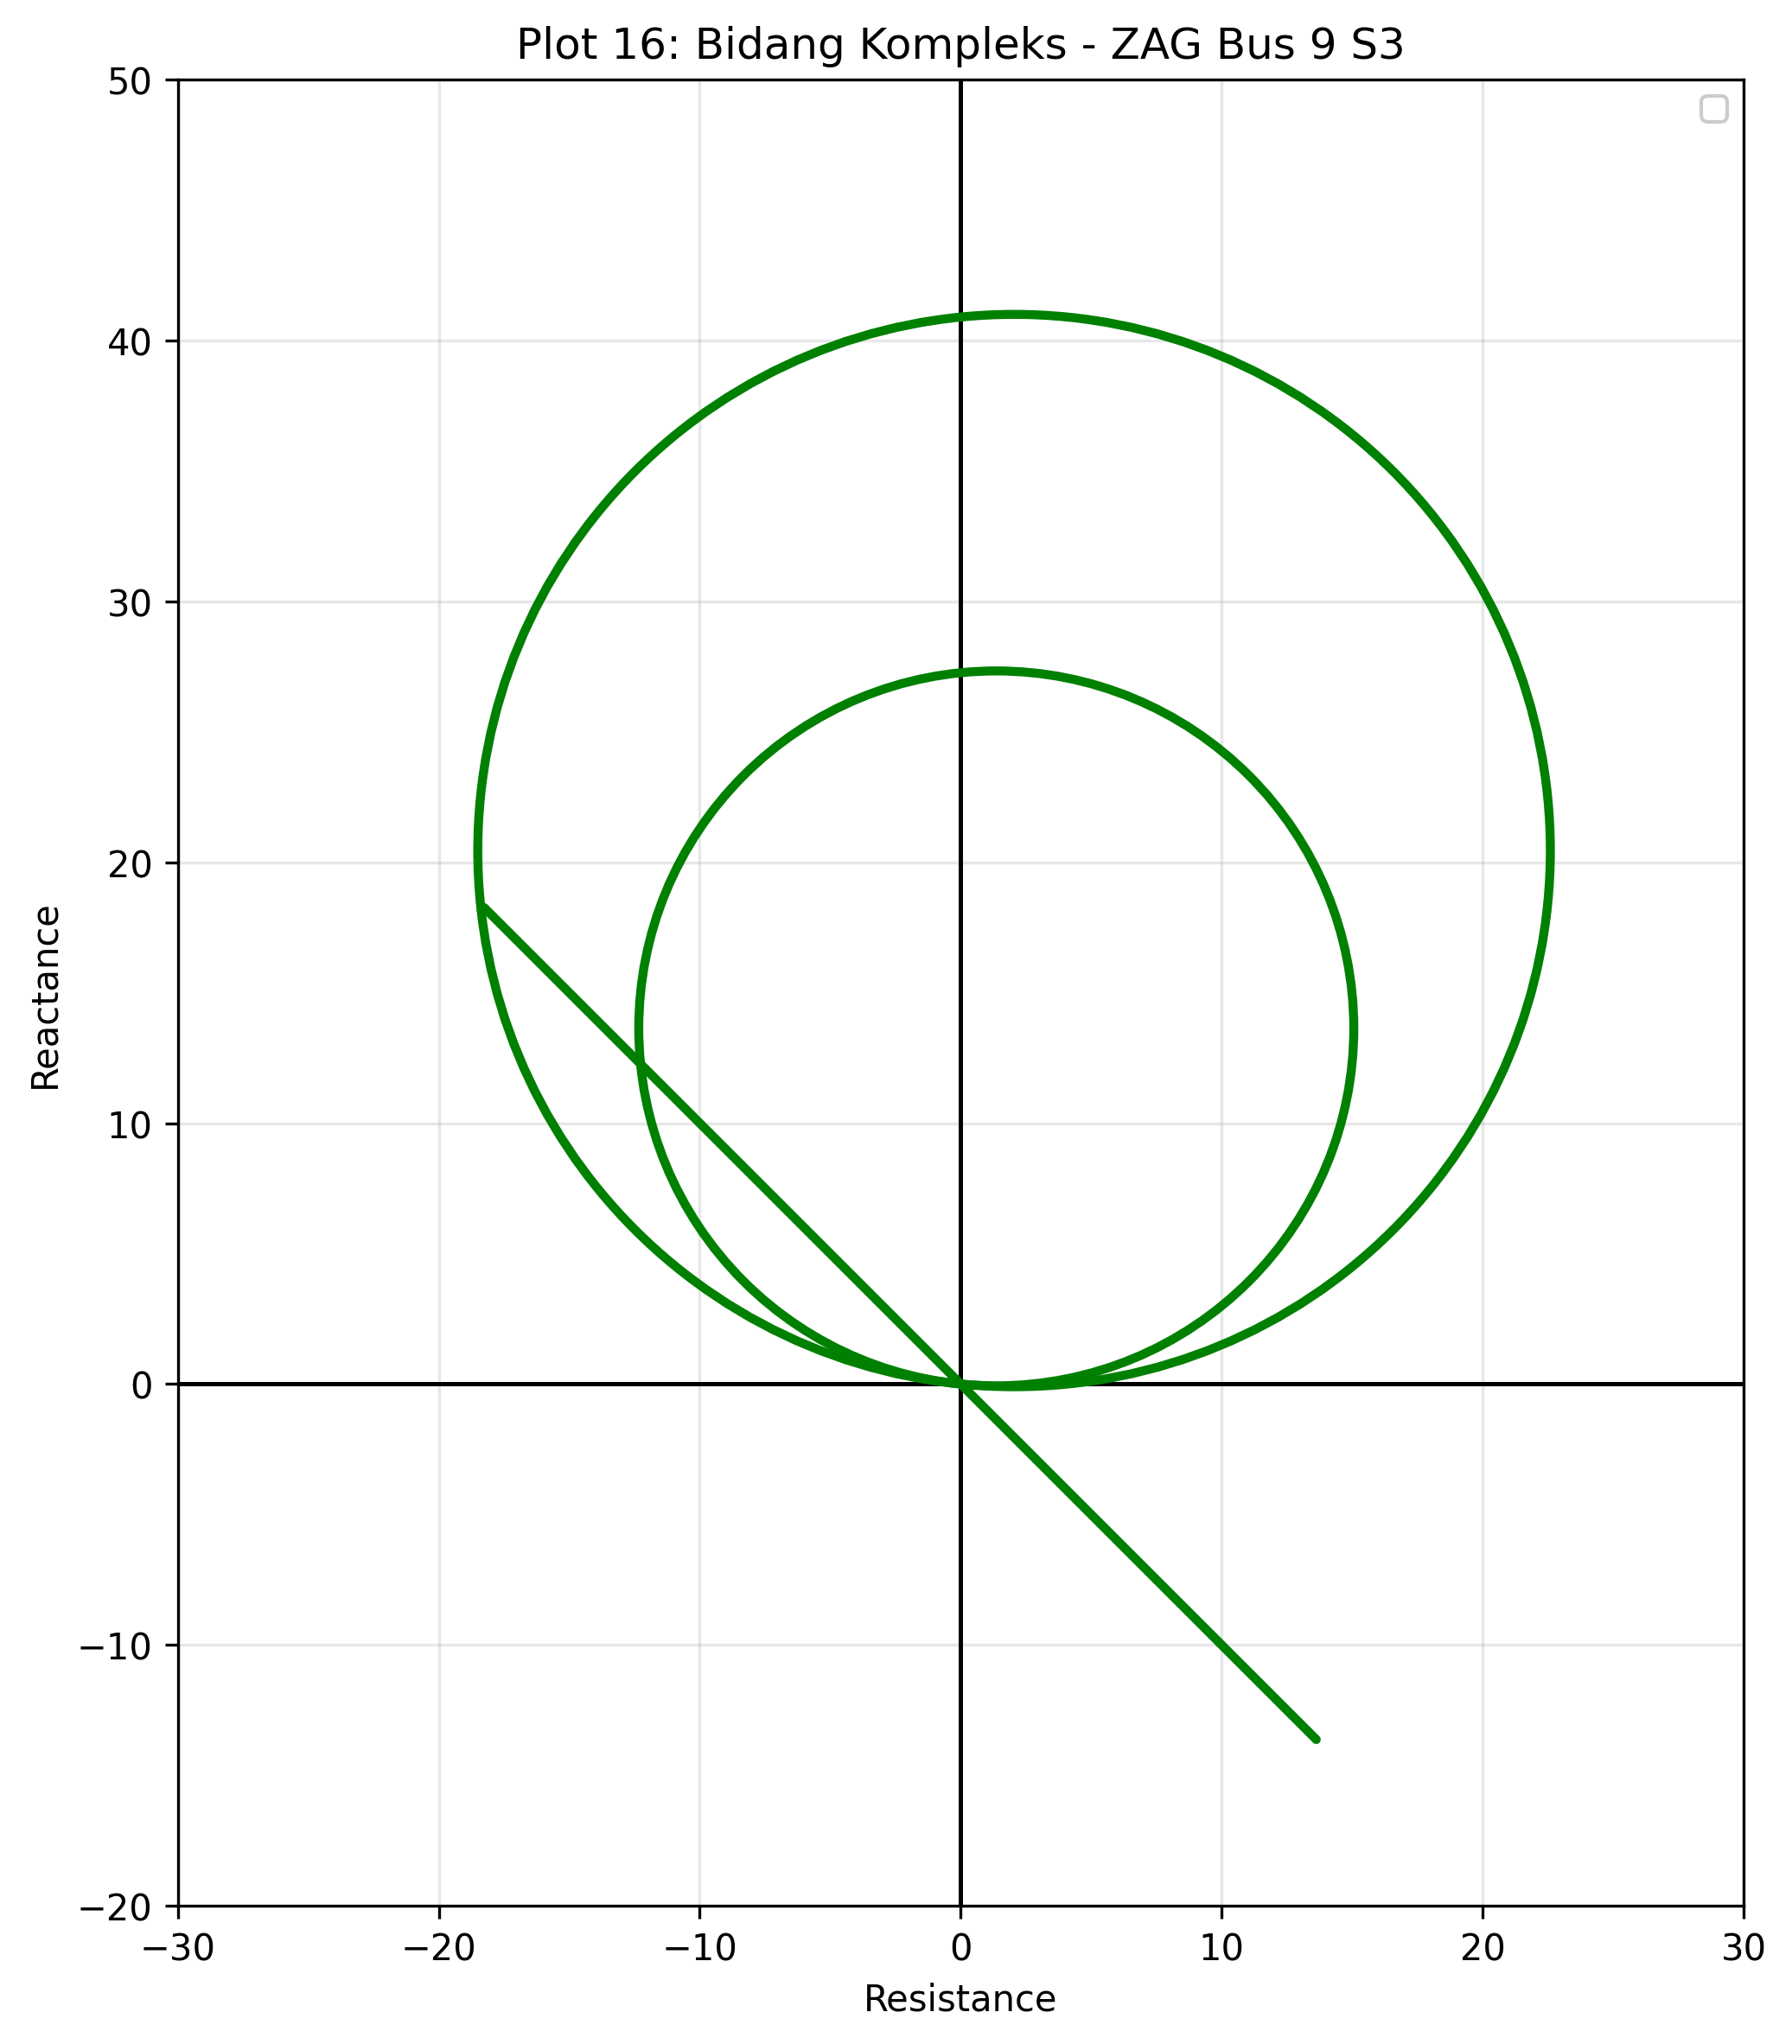
\includegraphics[width=0.8\textwidth]{contents/chapter-4/PRIZI_16_ZAG_Bus_9_S3.png}
%     \caption{Impedansi Tampak ZAG Bus 9 Skenario 3}
%     \label{fig:PRIZI_16_ZAG_Bus_9_S3}
% \end{figure}

\begin{figure}[H]
    \centering

    % Gambar sebelah kiri
    \begin{subfigure}[t]{0.48\textwidth}
        \centering
        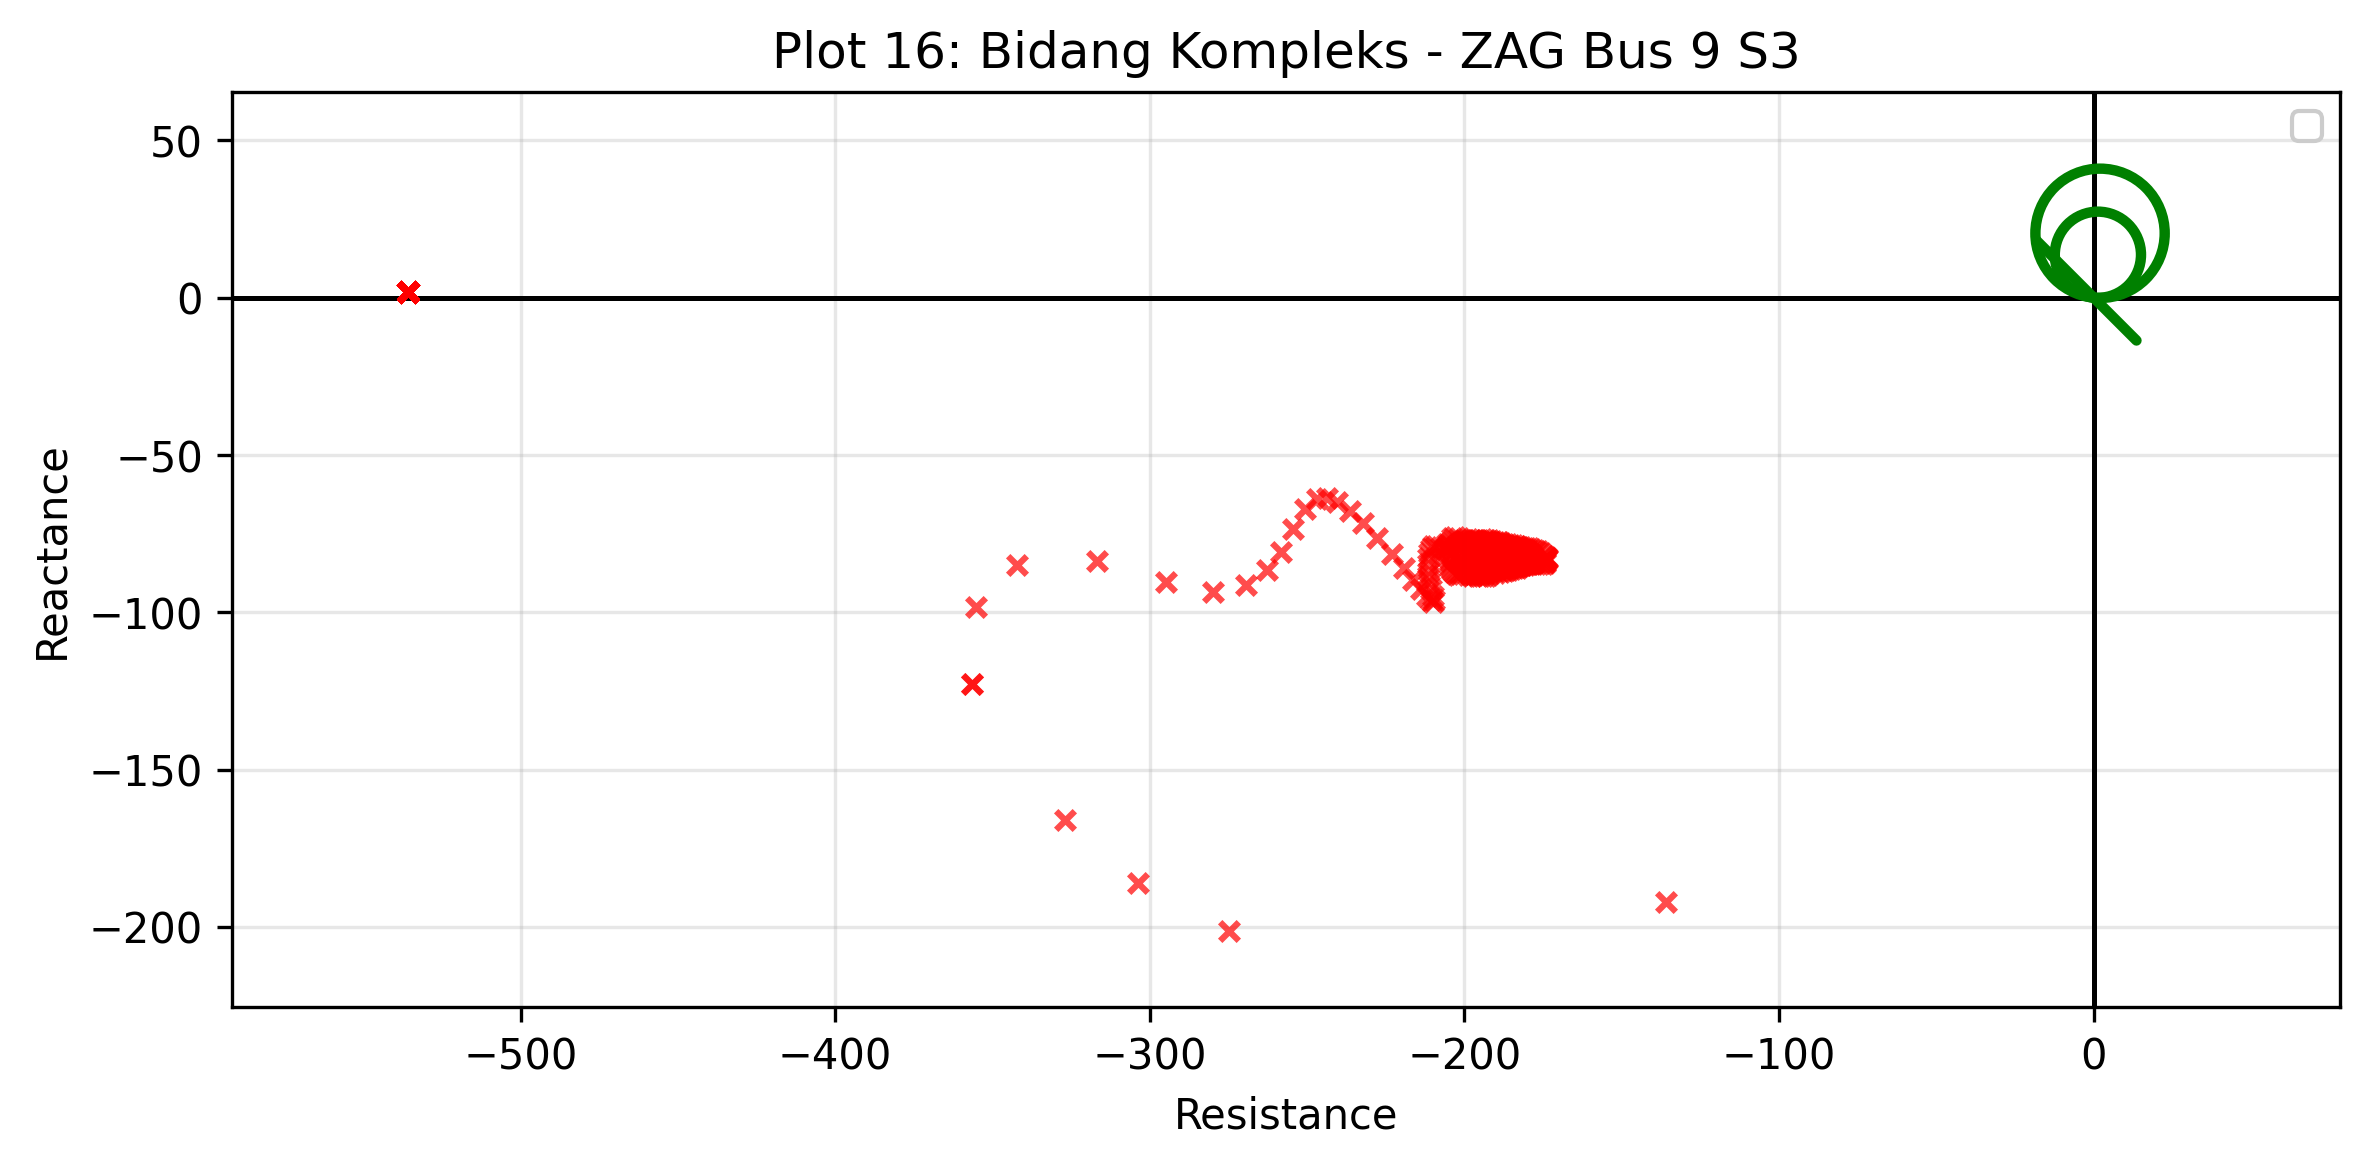
\includegraphics[width=\textwidth]{contents/chapter-4/PRIA_16_ZAG_Bus_9_S3.png}
        \caption{Seluruh Impedansi Tampak}
        \label{fig:PRIA_16_ZAG_Bus_9_S3}
    \end{subfigure}
    \hfill
    % Gambar sebelah kanan
    \begin{subfigure}[t]{0.48\textwidth}
        \centering
        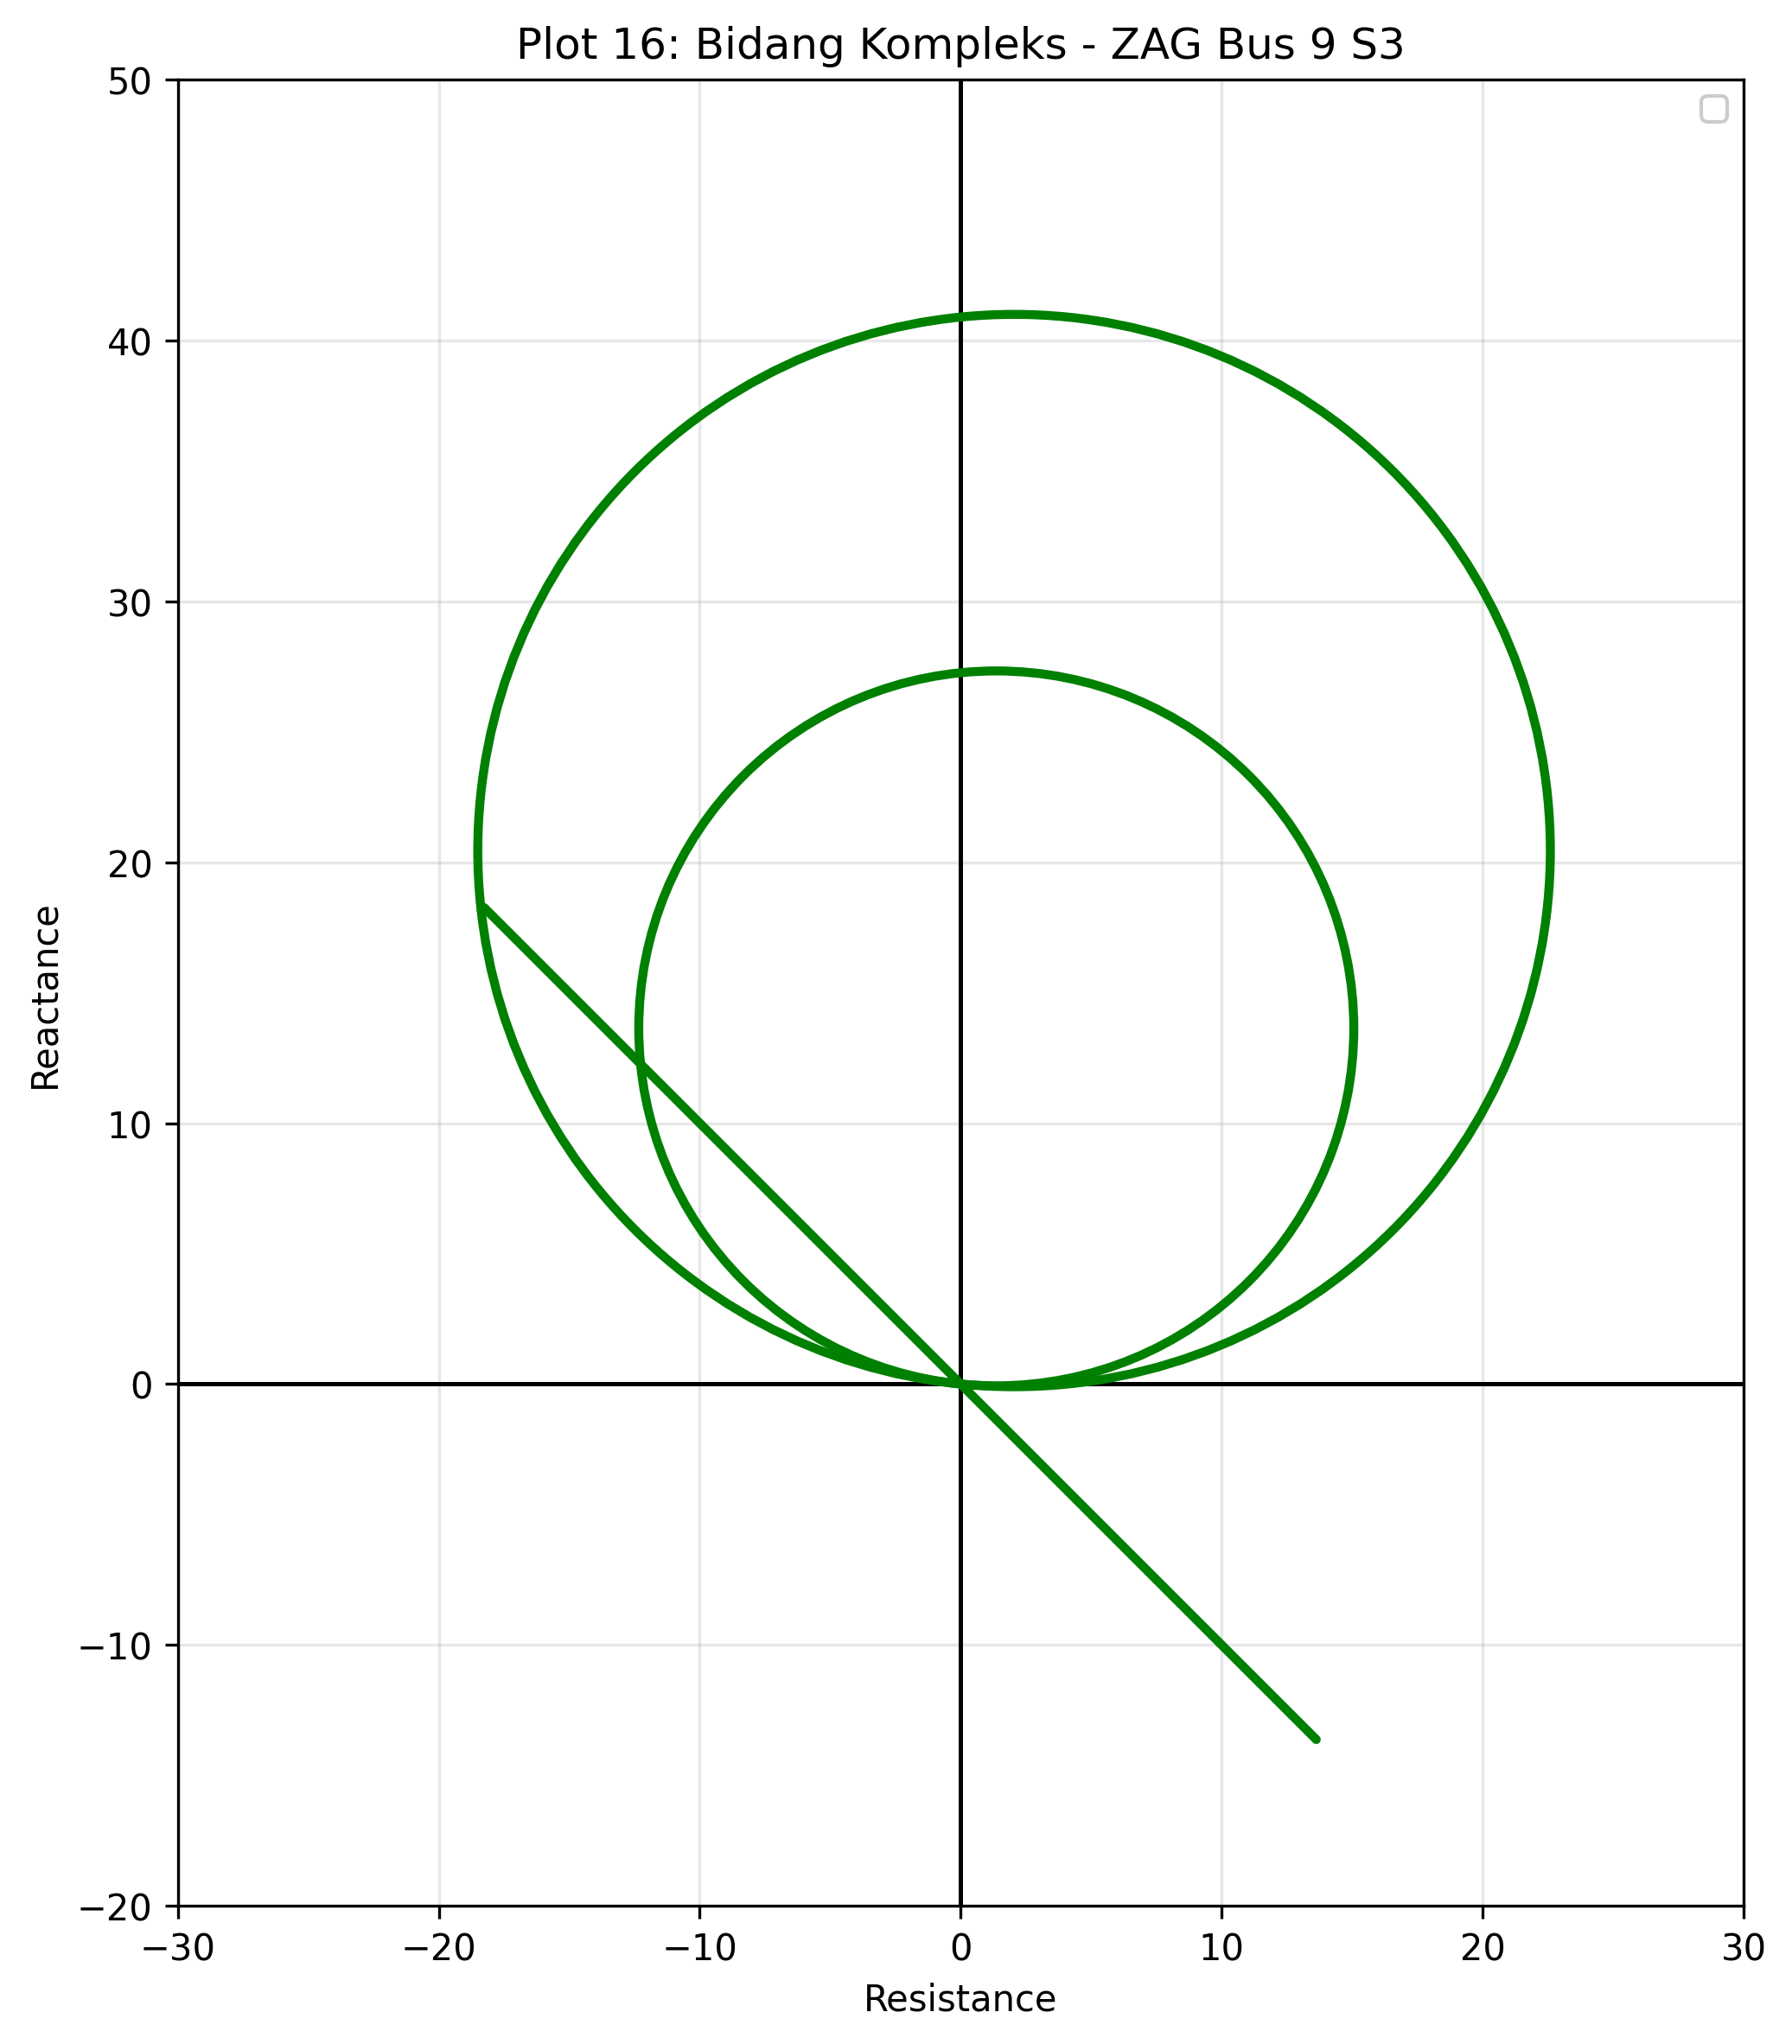
\includegraphics[width=\textwidth]{contents/chapter-4/PRIZI_16_ZAG_Bus_9_S3.png}
        \caption{Zoom In Pada Zona Proteksi}
        \label{fig:PRIZI_16_ZAG_Bus_9_S3}
    \end{subfigure}

    \caption{Impedansi Tampak ZAG Bus 9 Skenario 3}
    \label{fig:Impedansi_Tampak_ZAG_Bus_9_S3}
\end{figure}

Terlihat pada gambar \ref{fig:Impedansi_Tampak_ZAG_Bus_9_S3} bahwa impedansi tampak pada fasa A dengan ground yang dibaca oleh relay 21 sisi bus 9 saat terdapat gangguan bekerja dengan baik sesuai acuan pada \ref{subsec:tanpa_IBR_ex_dlg} relay 21 bus 9 tidak mendeteksi adanya gangguan sehingga tidak mengirimkan sinyal trip kepada CB.

%%%%%%%%%%%%%%%%%%%%%%%%%%%%%%%%%%%%%%%%%%%%%%%%%%%%%%%%%%%%%%%

% \begin{figure}[H]
%     \centering
%     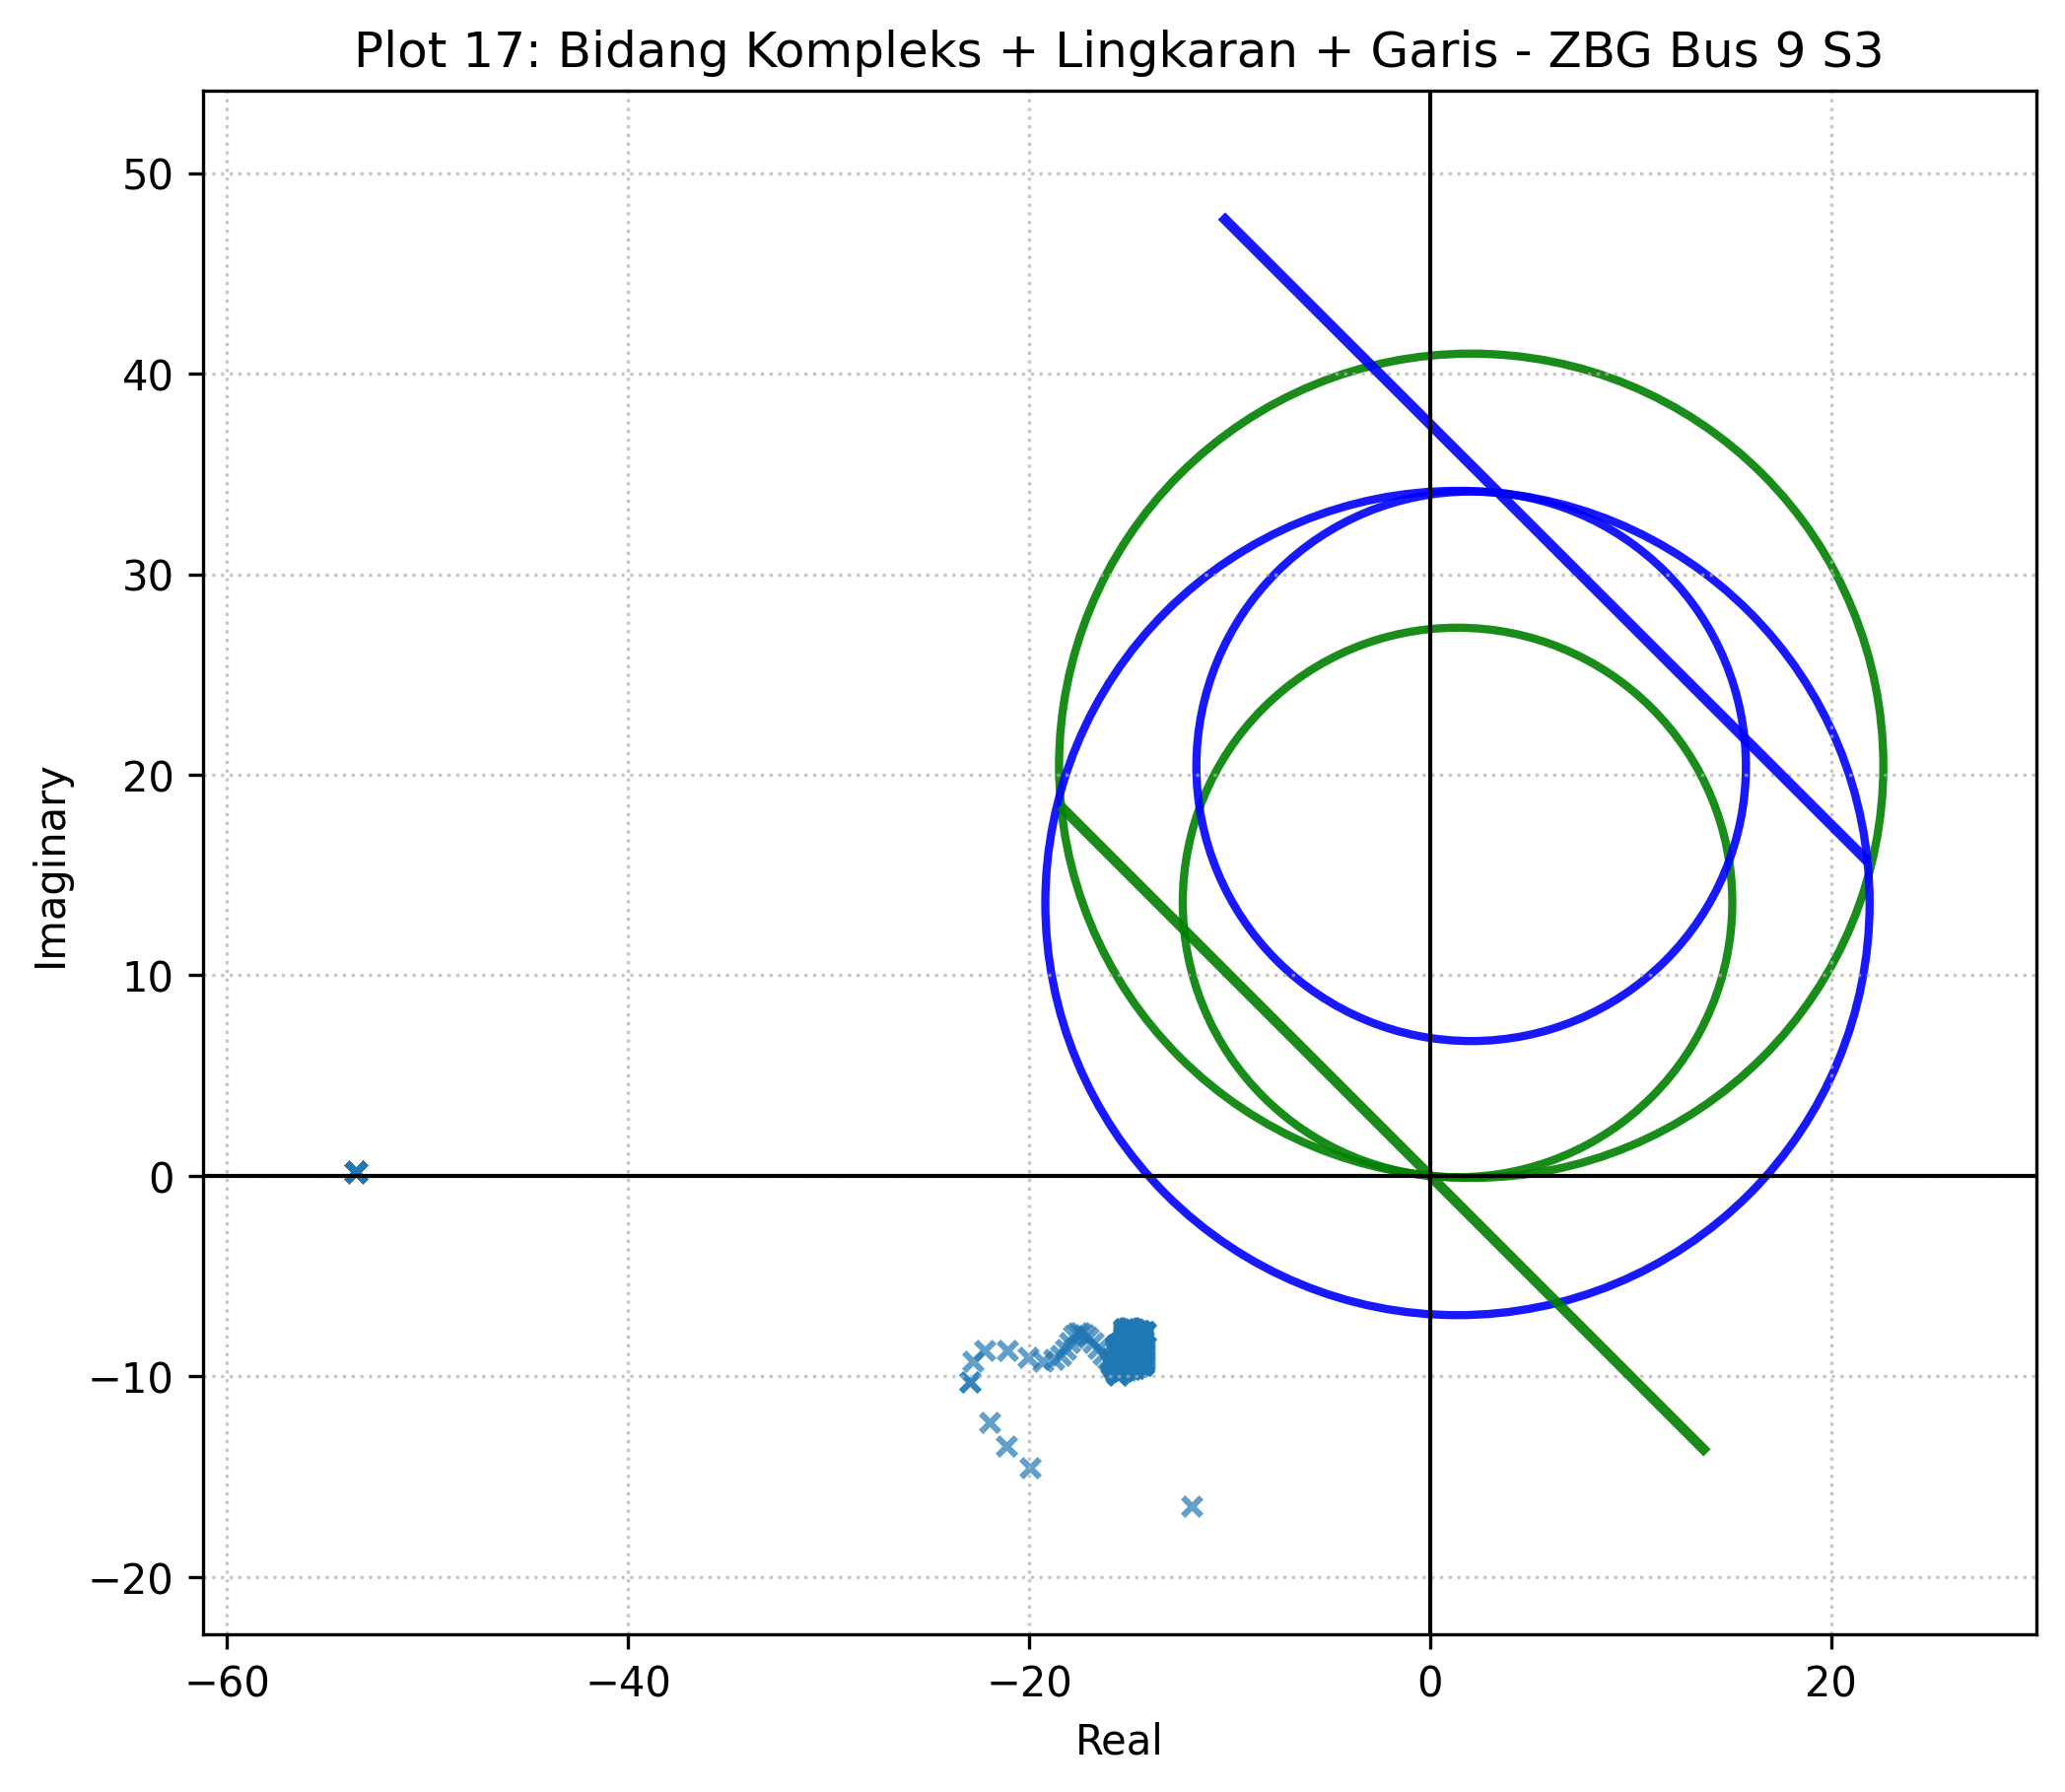
\includegraphics[width=0.8\textwidth]{contents/chapter-4/17_ZBG_Bus_9_S3_dengan_lingkaran_dan_garis.png}
%     \caption{Impedansi Tampak ZBG Bus 9 Skenario 3}
%     \label{fig:17_ZBG_Bus_9_S3_dengan_lingkaran_dan_garis}
% \end{figure}

% Terlihat pada gambar \ref{fig:17_ZBG_Bus_9_S3_dengan_lingkaran_dan_garis} bahwa impedansi tampak pada fasa B dengan ground yang dibaca oleh relay 21 sisi bus 9 saat terdapat gangguan bekerja dengan baik sesuai acuan pada \ref{subsec:tanpa_IBR_ex_dlg} relay 21 bus 9 tidak mendeteksi adanya gangguan sehingga tidak mengirimkan sinyal trip kepada CB.

%%%%%%%%%%%%%%%%%%%%%%%%%%%%%%%%%SISI PRIMER%%%%%%%%%%%%%%%%%%%%%%%%%%%%%%%%%%

% \begin{figure}[H]
%     \centering
%     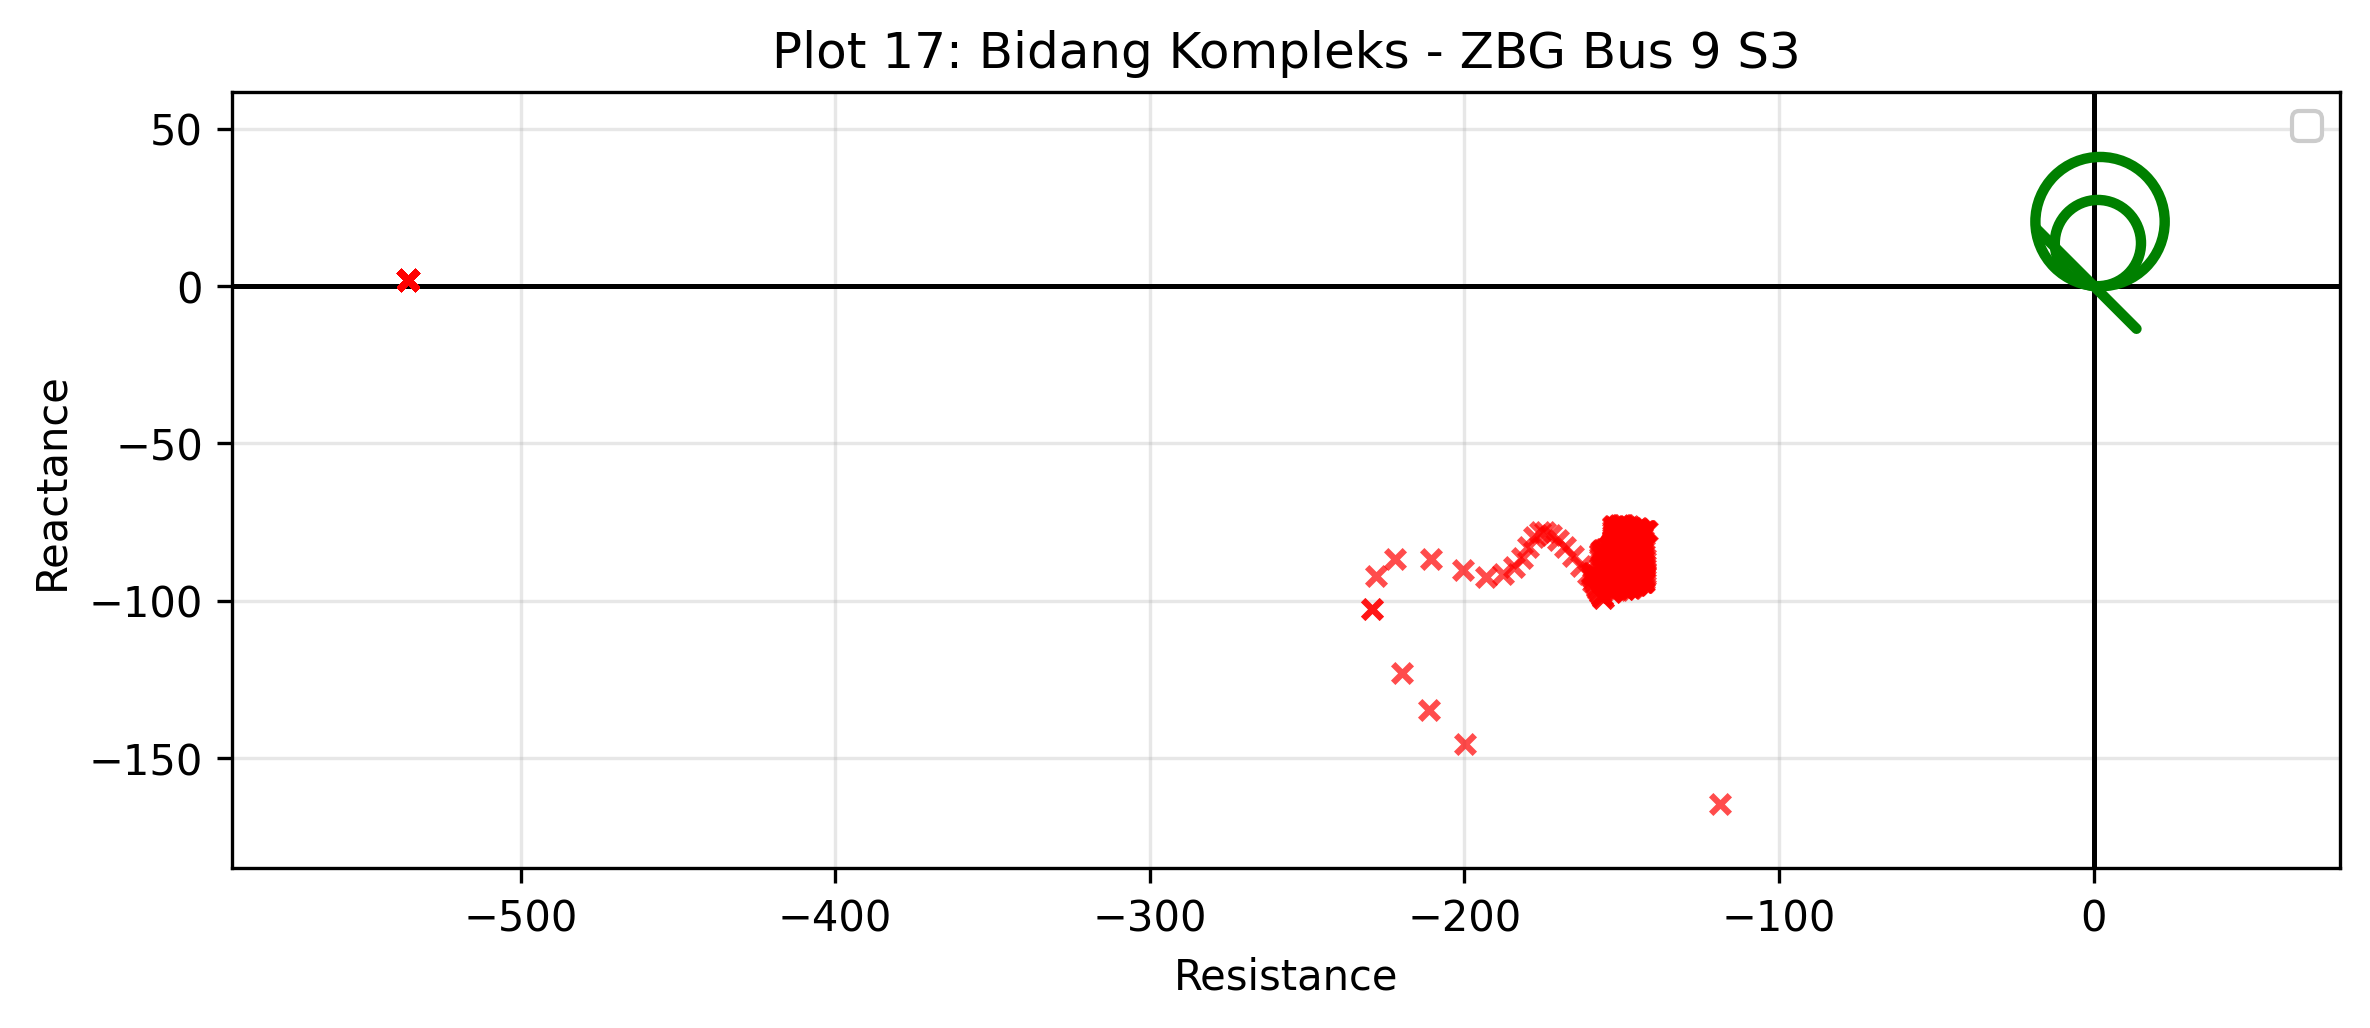
\includegraphics[width=0.8\textwidth]{contents/chapter-4/PRIA_17_ZBG_Bus_9_S3.png}
%     \caption{Impedansi Tampak ZBG Bus 9 Skenario 3}
%     \label{fig:PRIA_17_ZBG_Bus_9_S3}
% \end{figure}

% \begin{figure}[H]
%     \centering
%     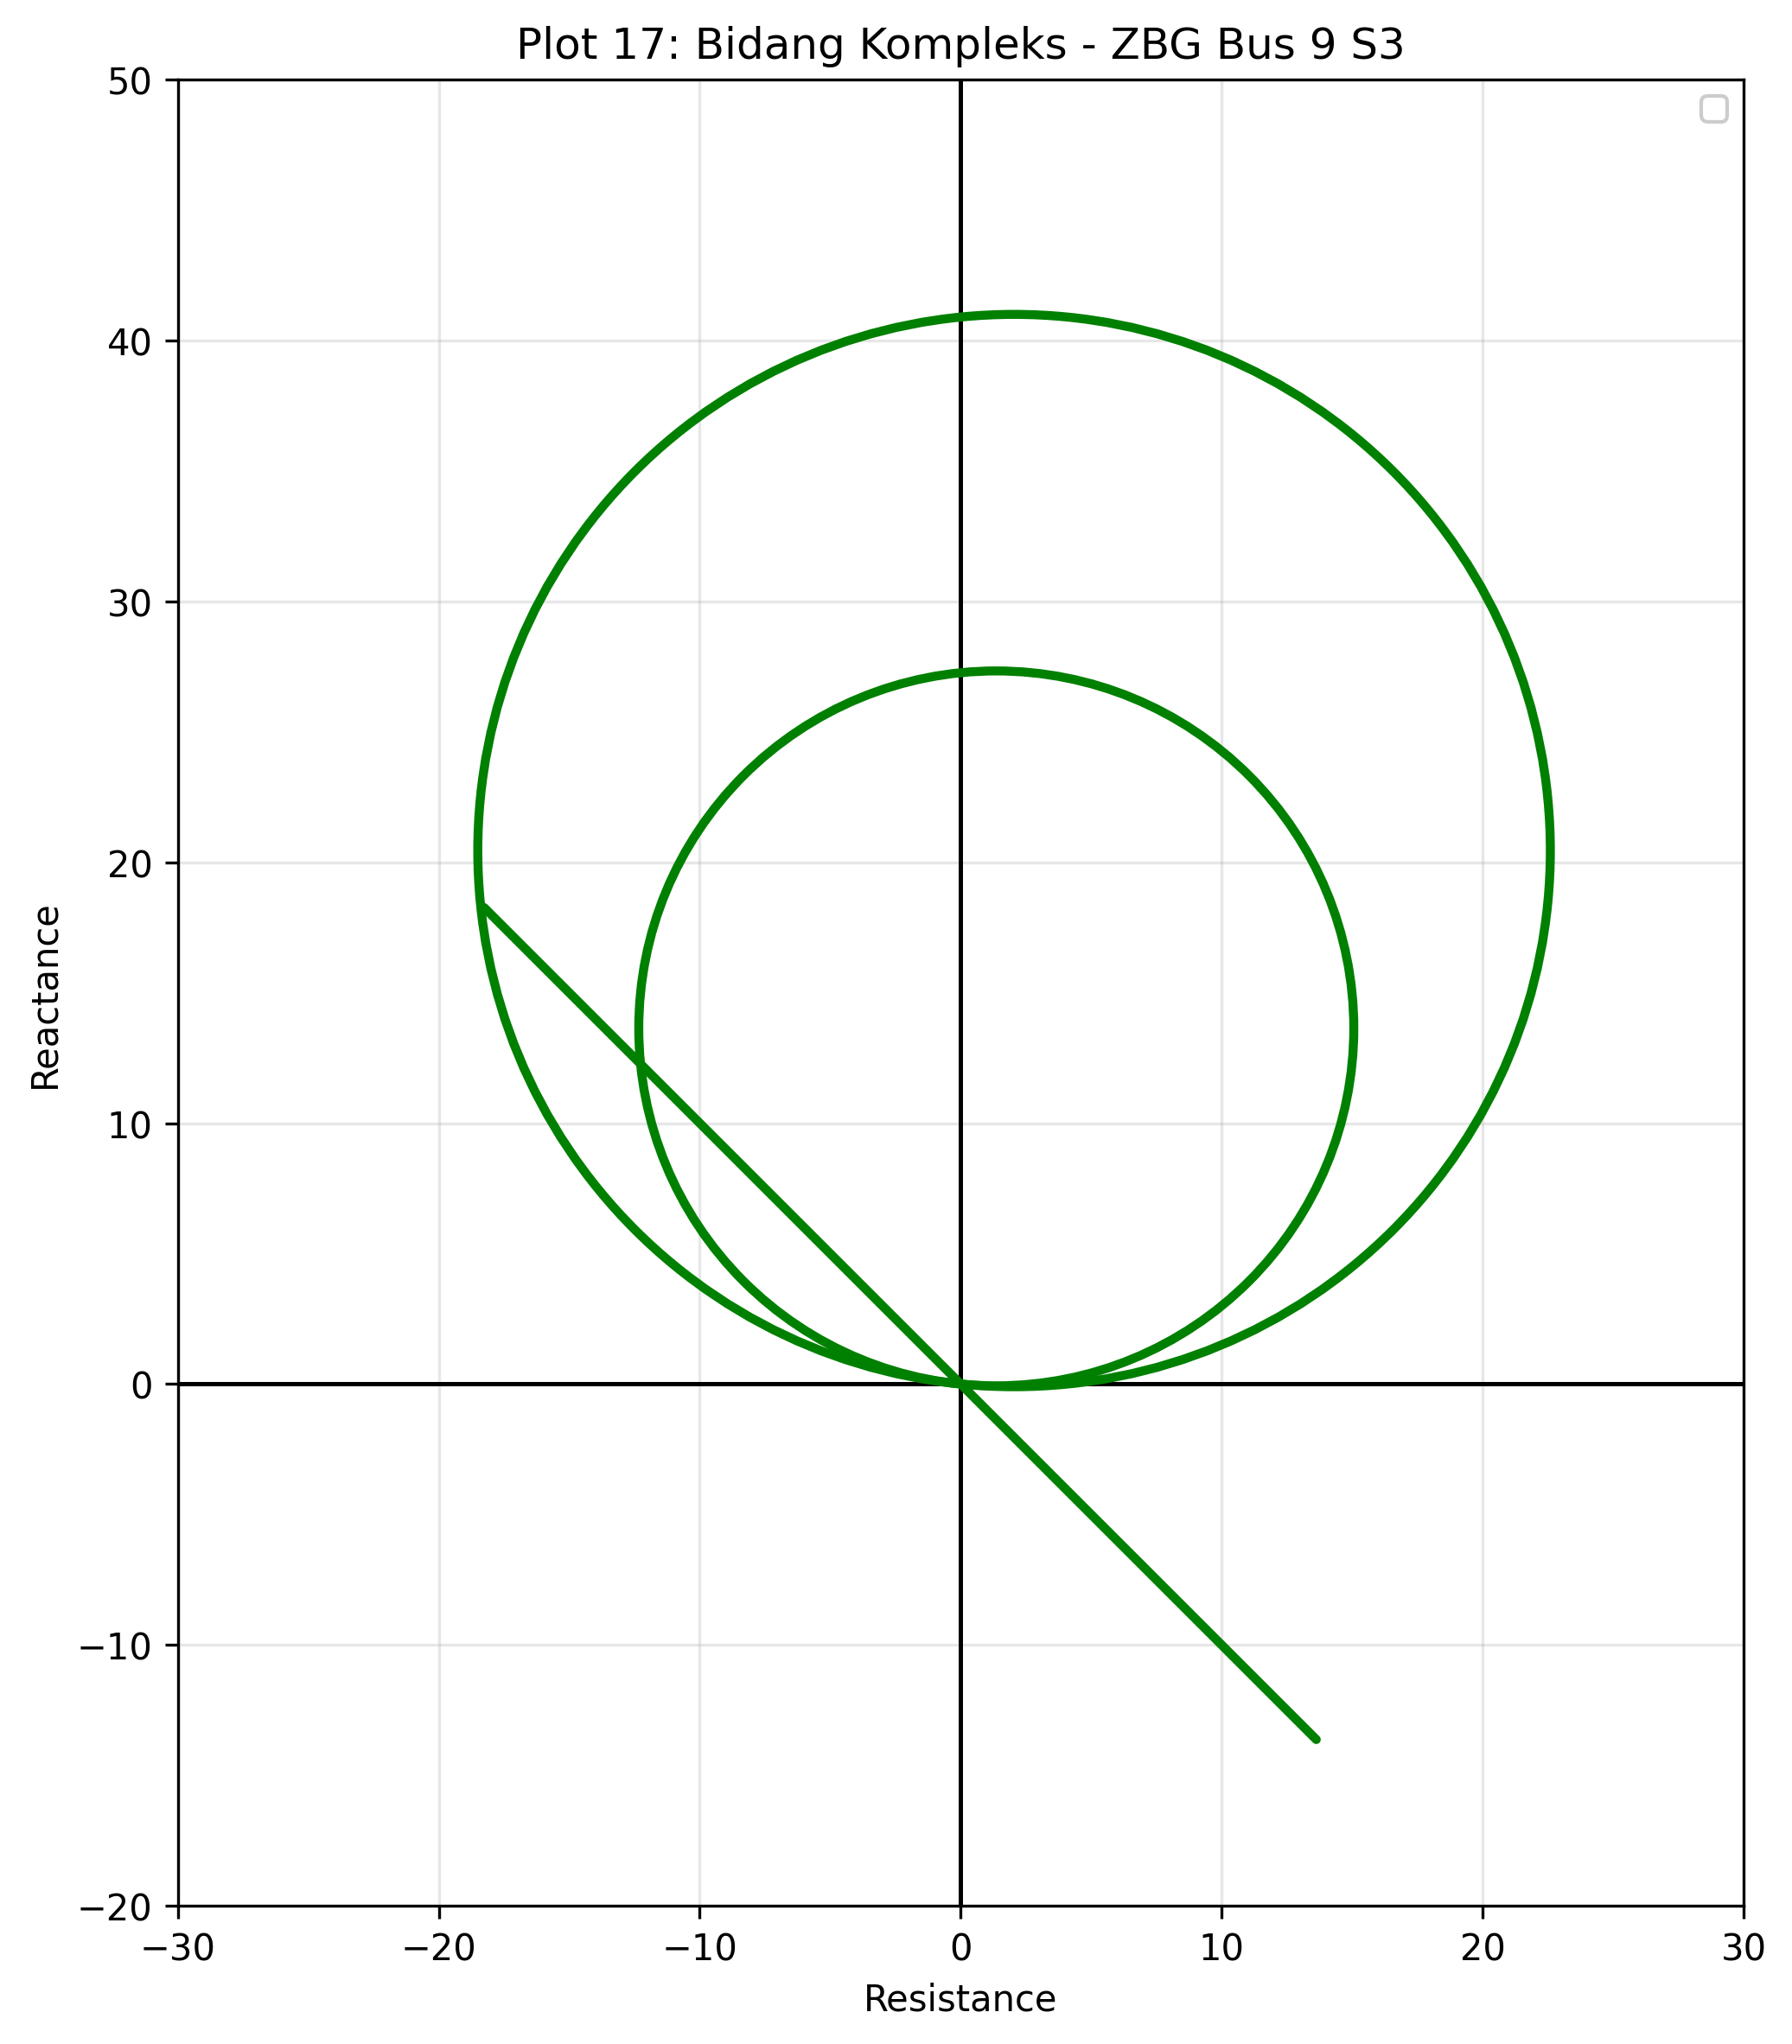
\includegraphics[width=0.8\textwidth]{contents/chapter-4/PRIZI_17_ZBG_Bus_9_S3.png}
%     \caption{Impedansi Tampak ZBG Bus 9 Skenario 3}
%     \label{fig:PRIZI_17_ZBG_Bus_9_S3}
% \end{figure}

\begin{figure}[H]
    \centering

    % Gambar sebelah kiri
    \begin{subfigure}[t]{0.48\textwidth}
        \centering
        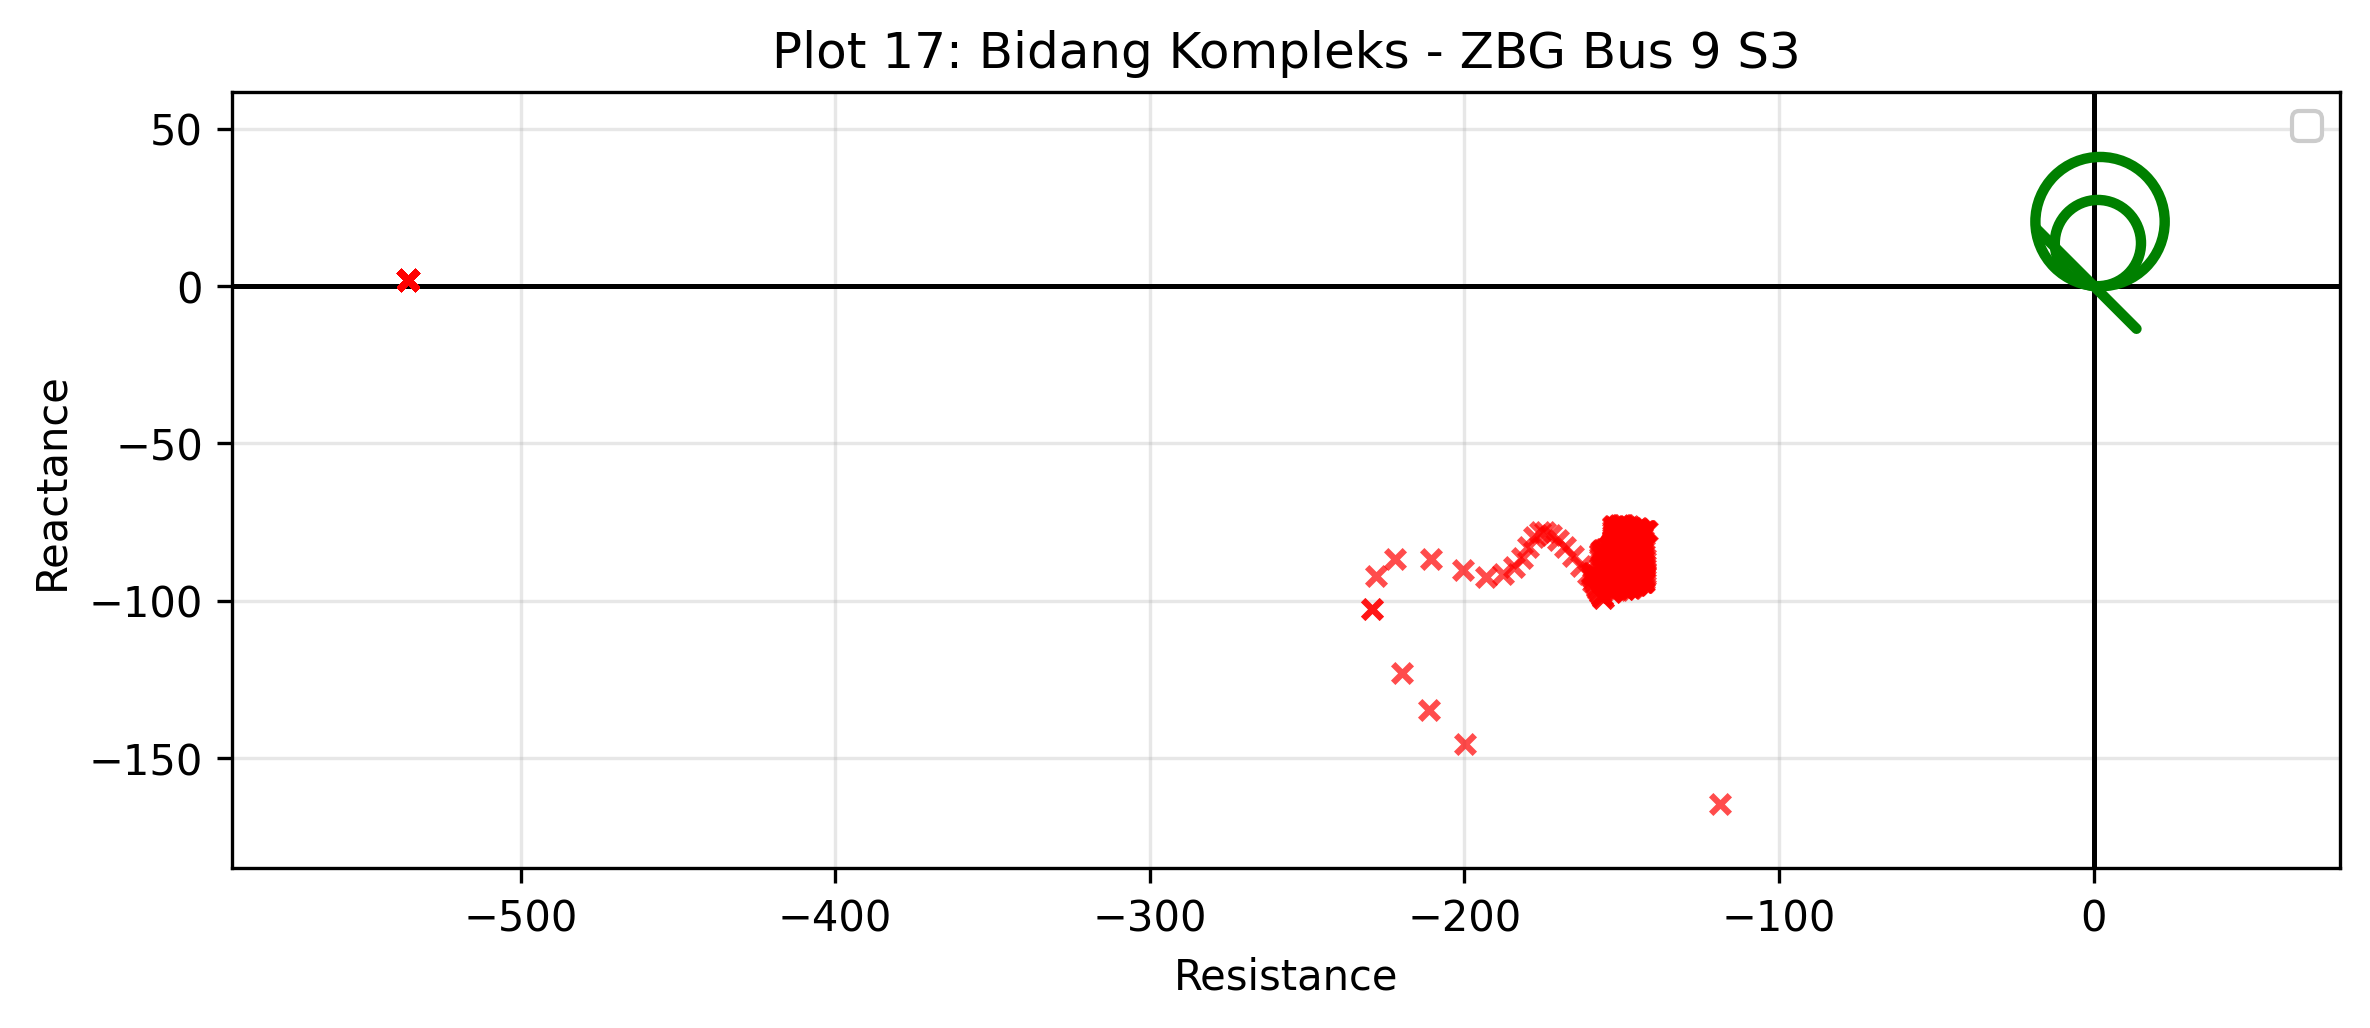
\includegraphics[width=\textwidth]{contents/chapter-4/PRIA_17_ZBG_Bus_9_S3.png}
        \caption{Seluruh Impedansi Tampak}
        \label{fig:PRIA_17_ZBG_Bus_9_S3}
    \end{subfigure}
    \hfill
    % Gambar sebelah kanan
    \begin{subfigure}[t]{0.48\textwidth}
        \centering
        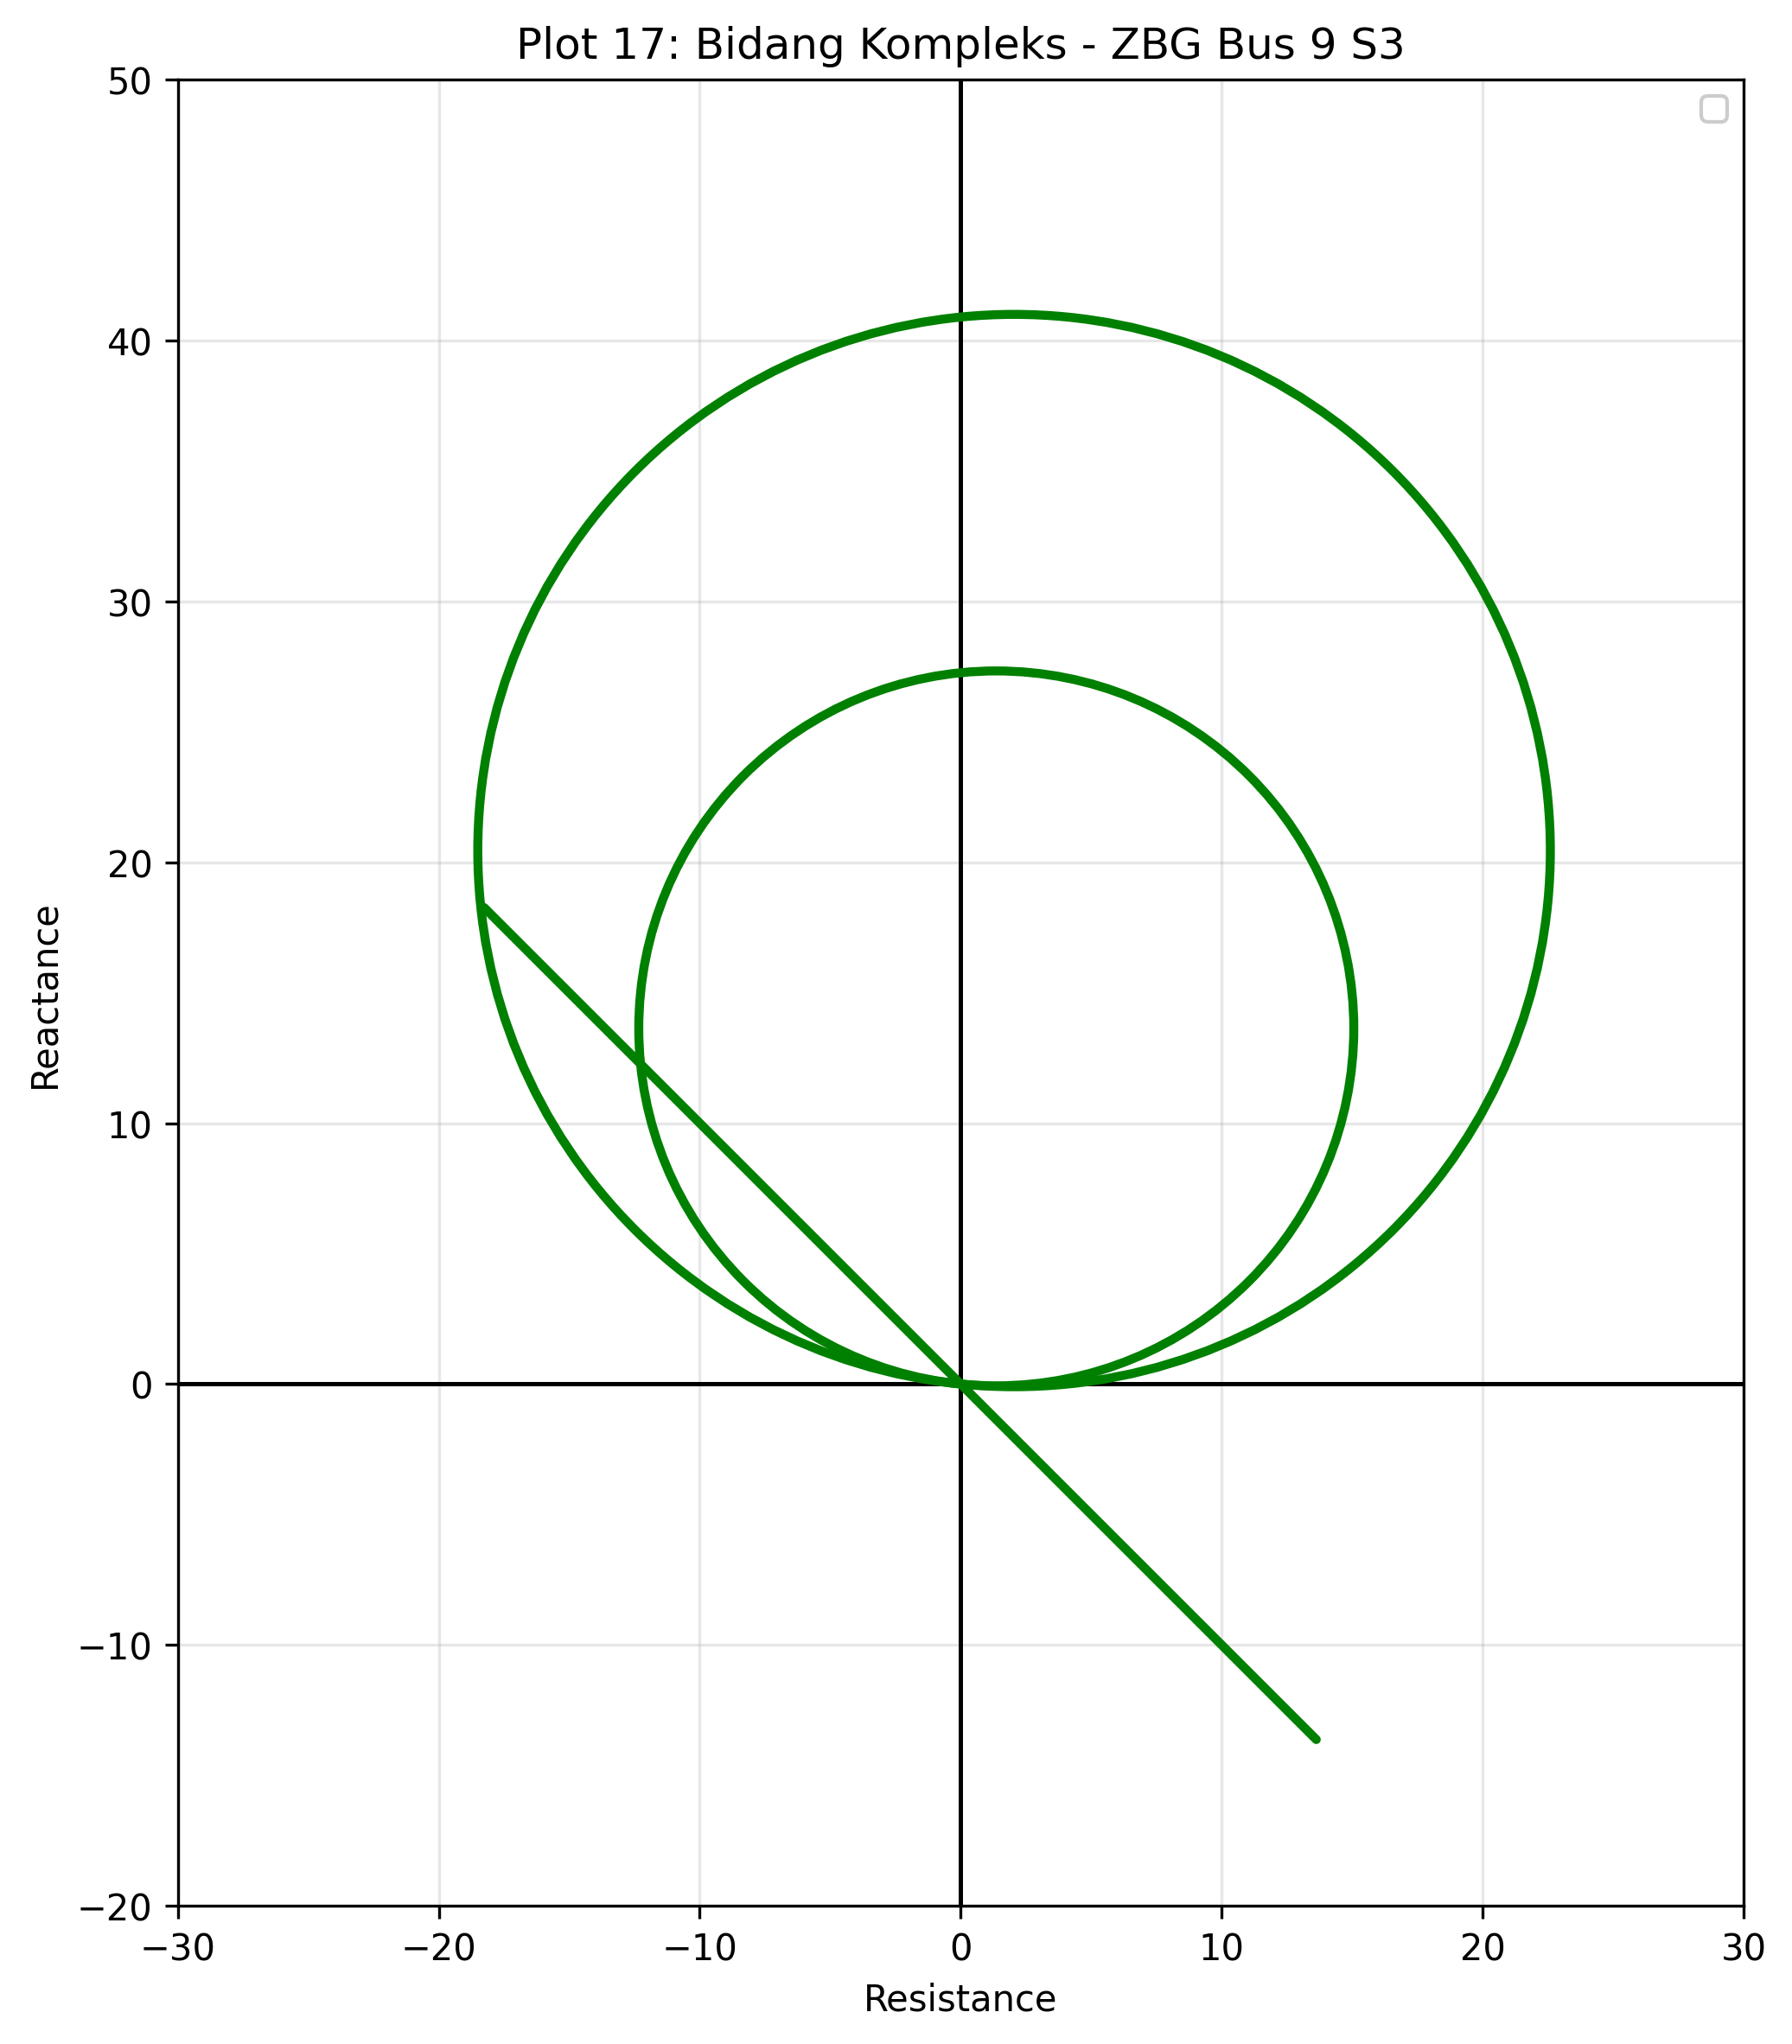
\includegraphics[width=\textwidth]{contents/chapter-4/PRIZI_17_ZBG_Bus_9_S3.png}
        \caption{Zoom In Pada Zona Proteksi}
        \label{fig:PRIZI_17_ZBG_Bus_9_S3}
    \end{subfigure}

    \caption{Impedansi Tampak ZBG Bus 9 Skenario 3}
    \label{fig:Impedansi_Tampak_ZBG_Bus_9_S3}
\end{figure}

Terlihat pada gambar \ref{fig:Impedansi_Tampak_ZBG_Bus_9_S3} bahwa impedansi tampak pada fasa B dengan ground yang dibaca oleh relay 21 sisi bus 9 saat terdapat gangguan bekerja dengan baik sesuai acuan pada \ref{subsec:tanpa_IBR_ex_dlg} relay 21 bus 9 tidak mendeteksi adanya gangguan sehingga tidak mengirimkan sinyal trip kepada CB.

%%%%%%%%%%%%%%%%%%%%%%%%%%%%%%%%%%%%%%%%%%%%%%%%%%%%%%%%%%%%%%%

% \begin{figure}[H]
%     \centering
%     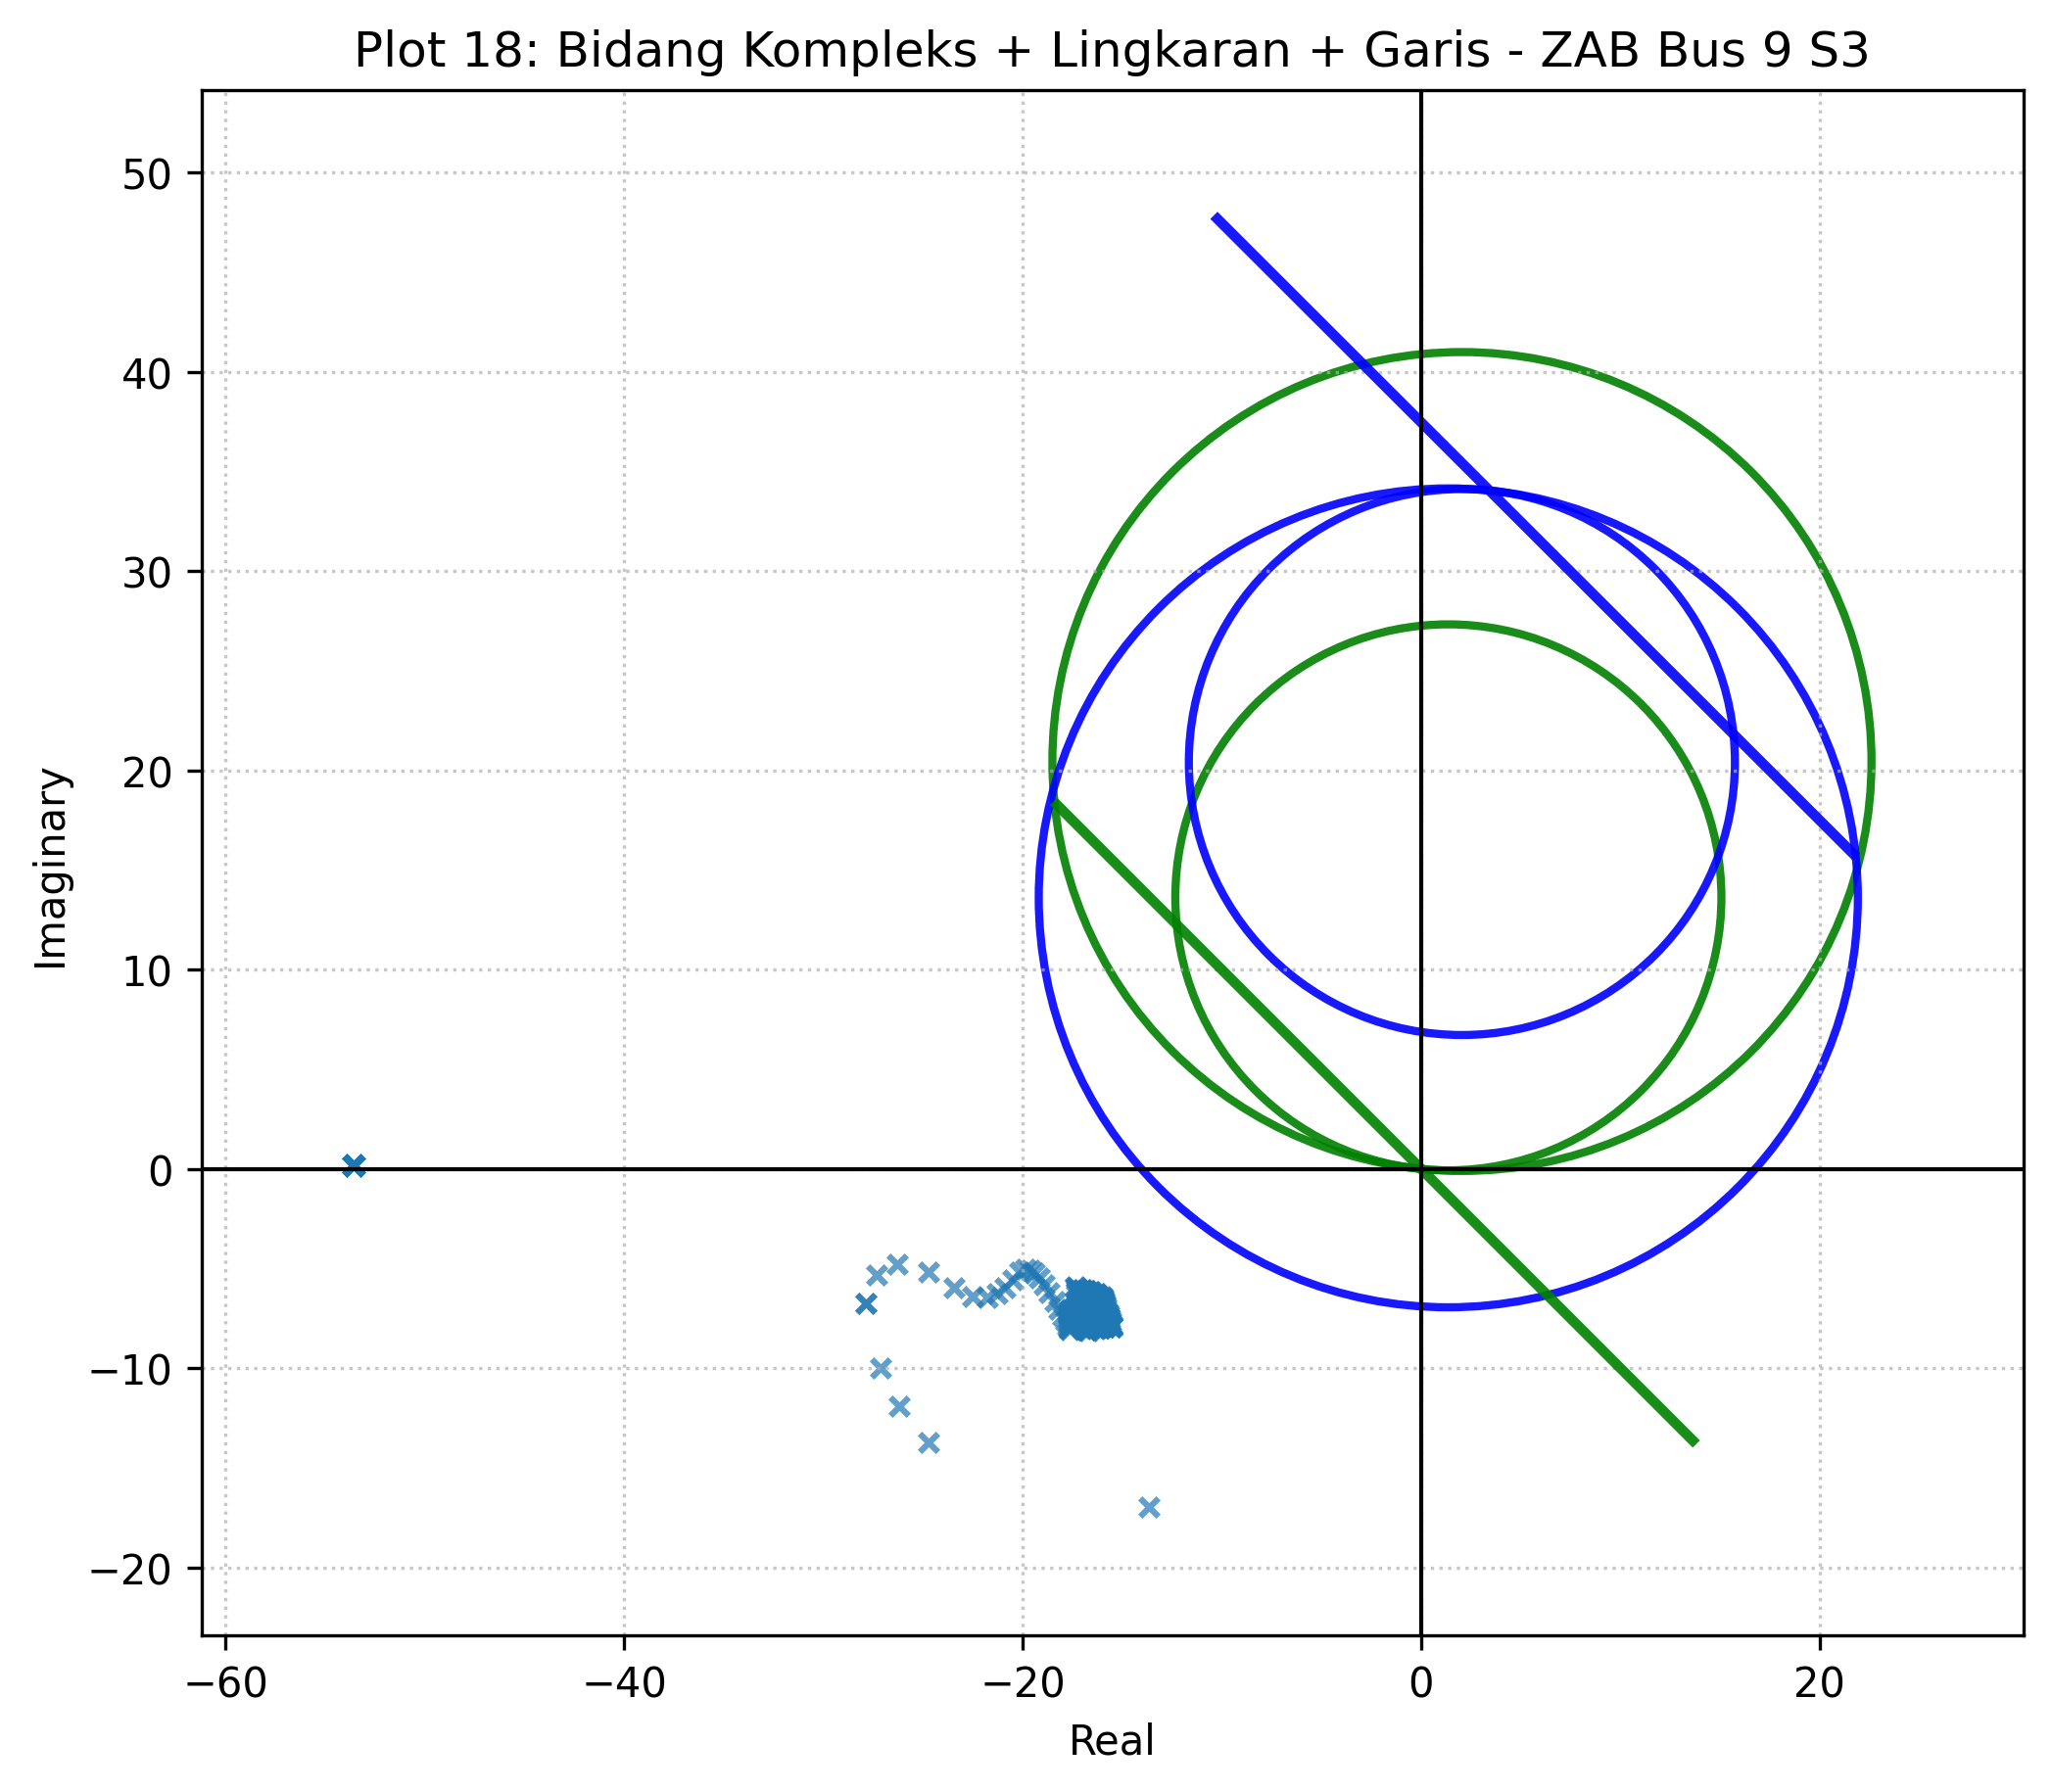
\includegraphics[width=0.8\textwidth]{contents/chapter-4/18_ZAB_Bus_9_S3_dengan_lingkaran_dan_garis.png}
%     \caption{Impedansi Tampak ZAB Bus 9 Skenario 3}
%     \label{fig:18_ZAB_Bus_9_S3_dengan_lingkaran_dan_garis}
% \end{figure}

% Terlihat pada gambar \ref{fig:18_ZAB_Bus_9_S3_dengan_lingkaran_dan_garis} bahwa impedansi tampak pada fasa A dengan fasa B yang dibaca oleh relay 21 sisi bus 9 saat terdapat gangguan bekerja dengan baik sesuai acuan pada \ref{subsec:tanpa_IBR_ex_dlg} relay 21 bus 9 tidak mendeteksi adanya gangguan sehingga tidak mengirimkan sinyal trip kepada CB.

%%%%%%%%%%%%%%%%%%%%%%%%%%%%%%%%%SISI PRIMER%%%%%%%%%%%%%%%%%%%%%%%%%%%%%%%%%%

% \begin{figure}[H]
%     \centering
%     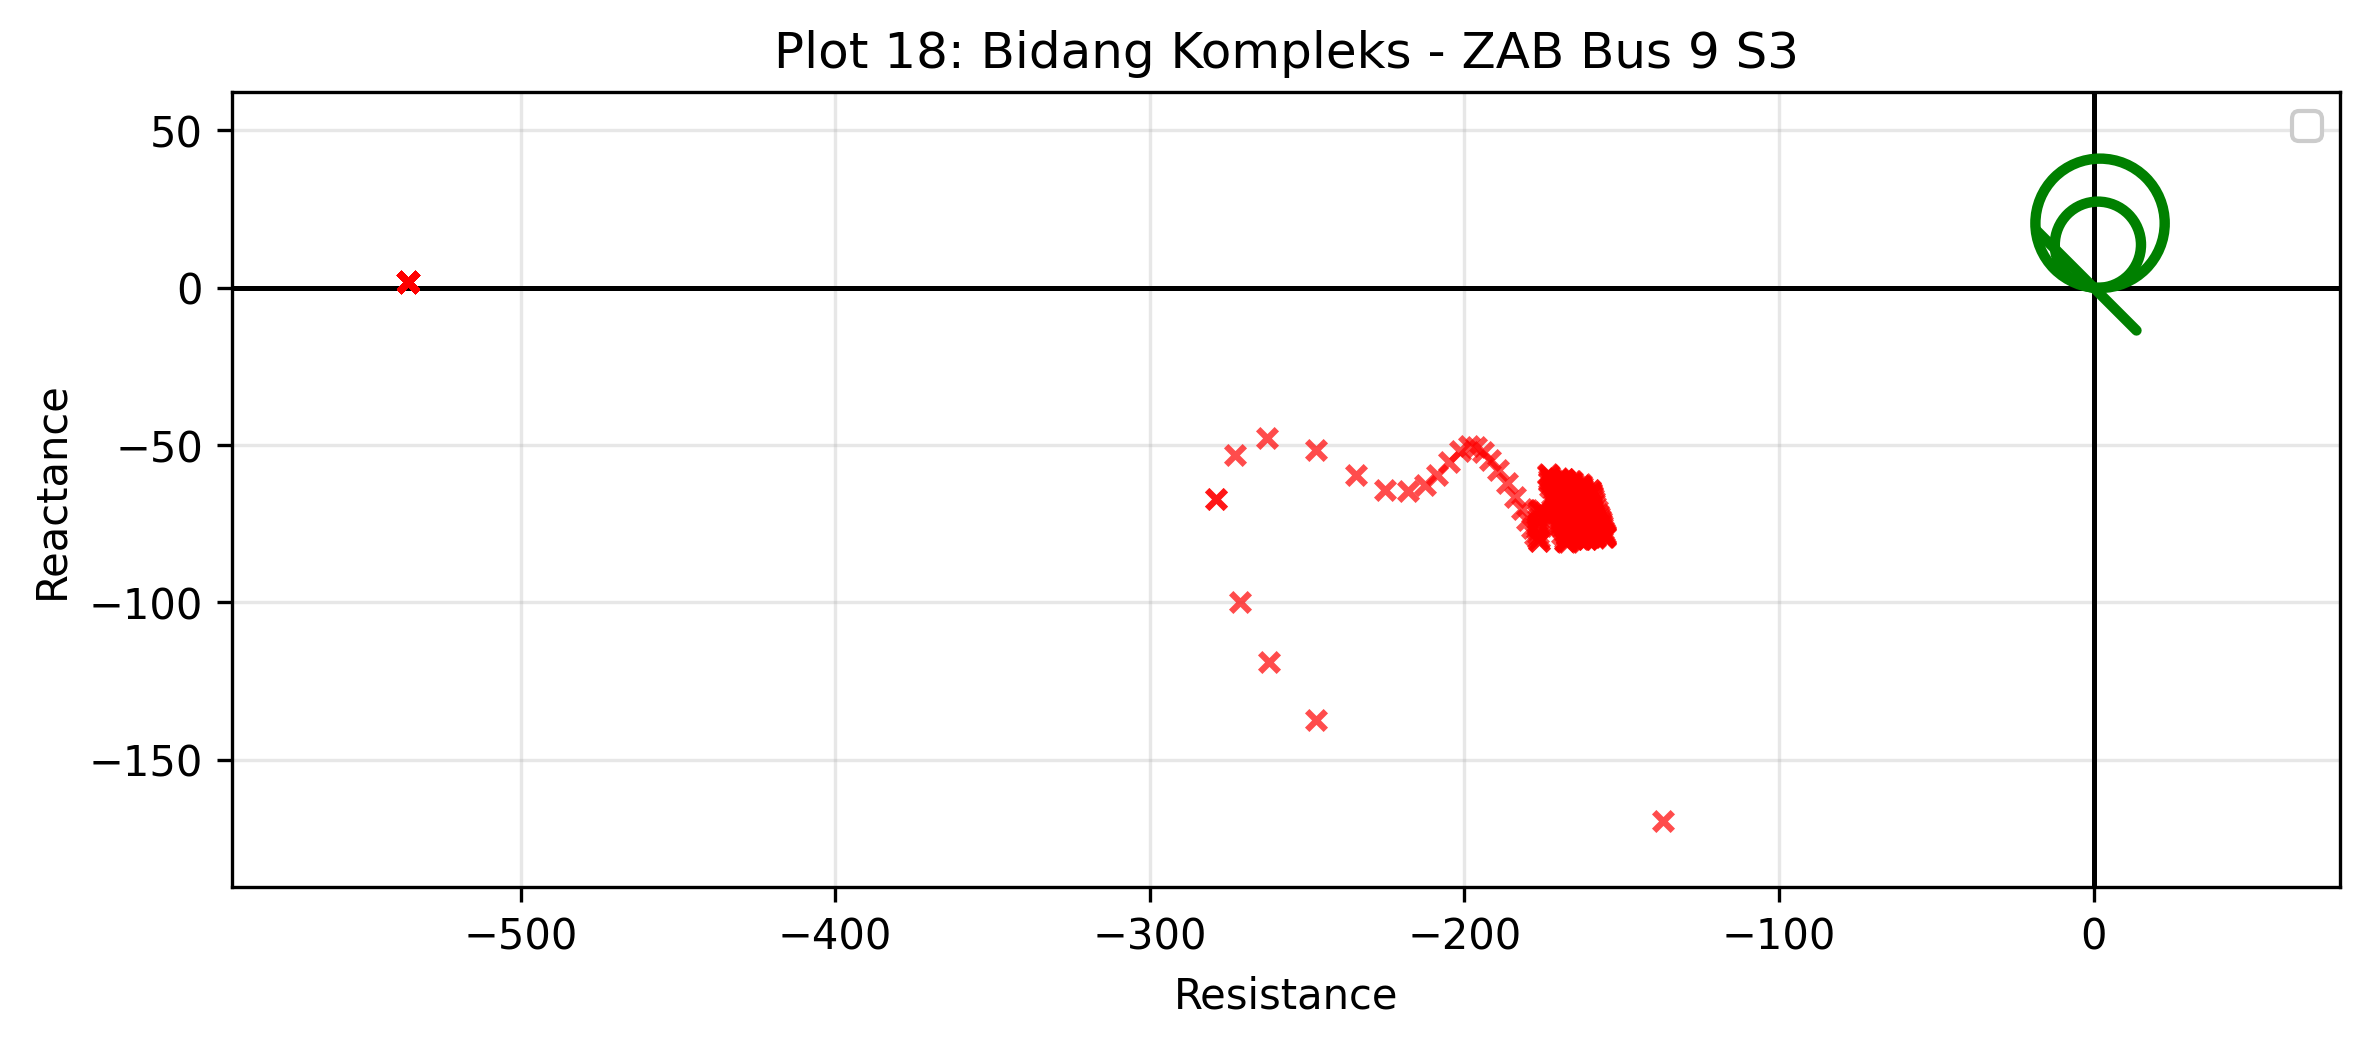
\includegraphics[width=0.8\textwidth]{contents/chapter-4/PRIA_18_ZAB_Bus_9_S3.png}
%     \caption{Impedansi Tampak ZAB Bus 9 Skenario 3}
%     \label{fig:PRIA_18_ZAB_Bus_9_S3}
% \end{figure}

% \begin{figure}[H]
%     \centering
%     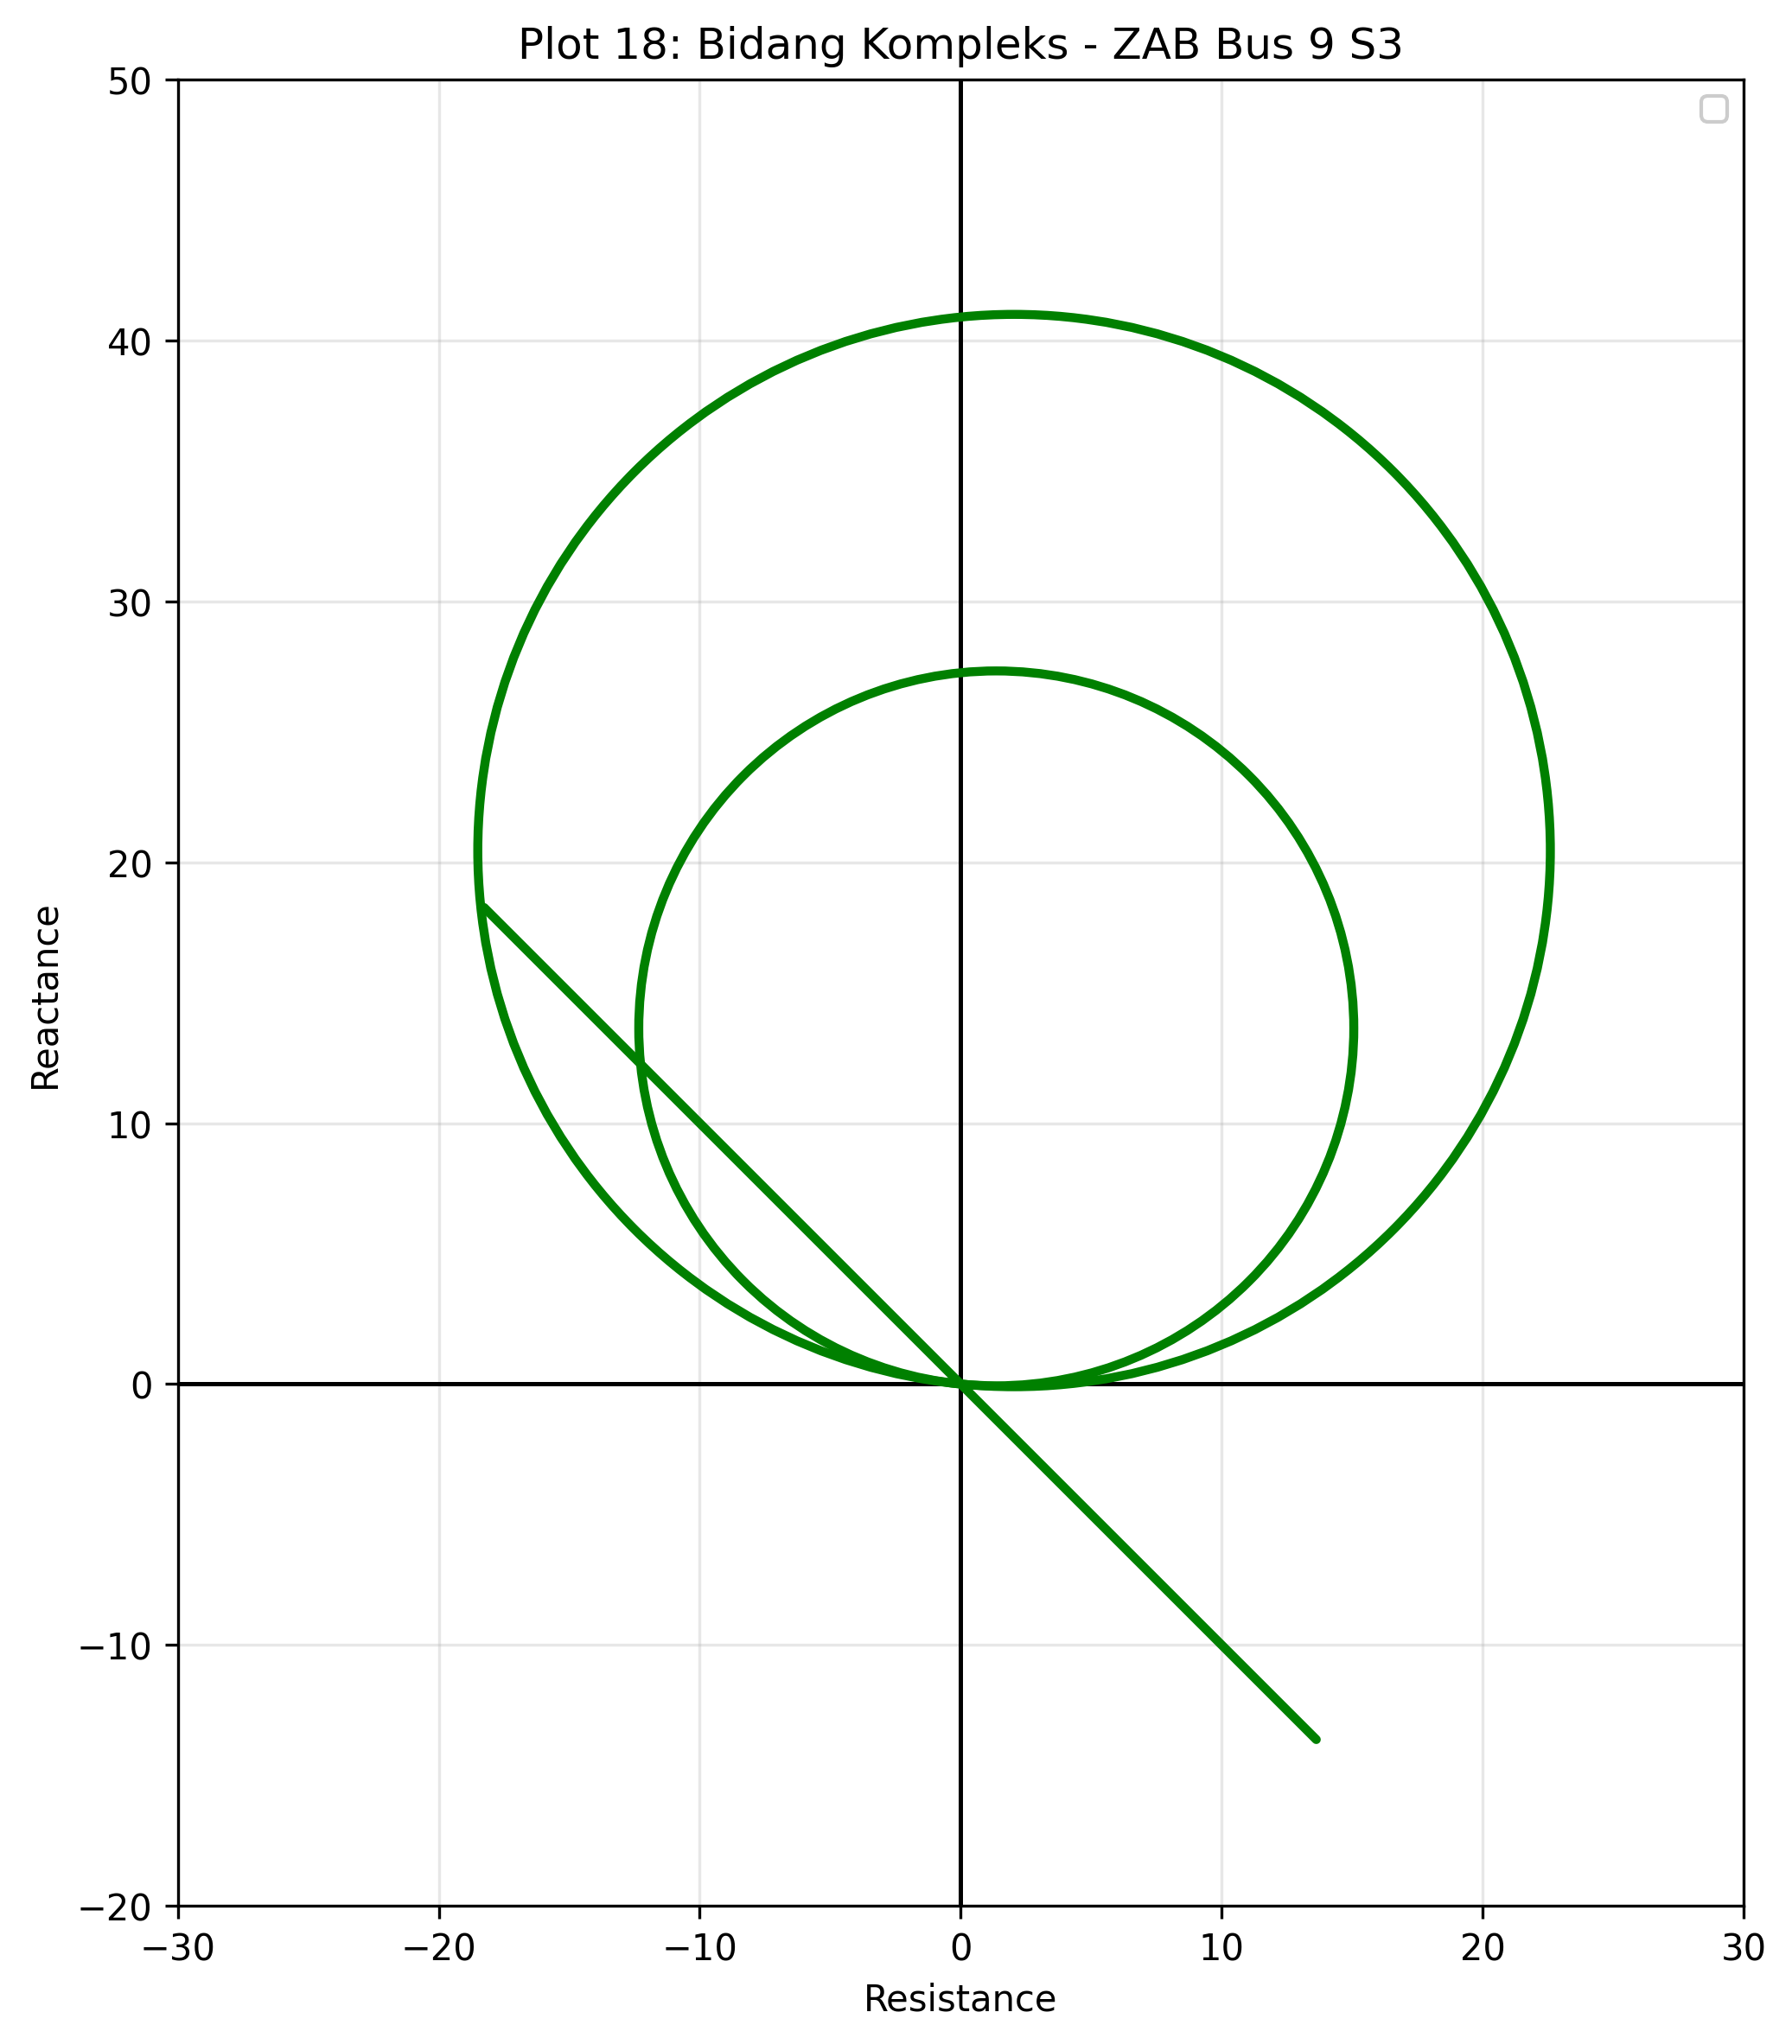
\includegraphics[width=0.8\textwidth]{contents/chapter-4/PRIZI_18_ZAB_Bus_9_S3.png}
%     \caption{Impedansi Tampak ZAB Bus 9 Skenario 3}
%     \label{fig:PRIZI_18_ZAB_Bus_9_S3}
% \end{figure}

\begin{figure}[H]
    \centering

    % Gambar sebelah kiri
    \begin{subfigure}[t]{0.48\textwidth}
        \centering
        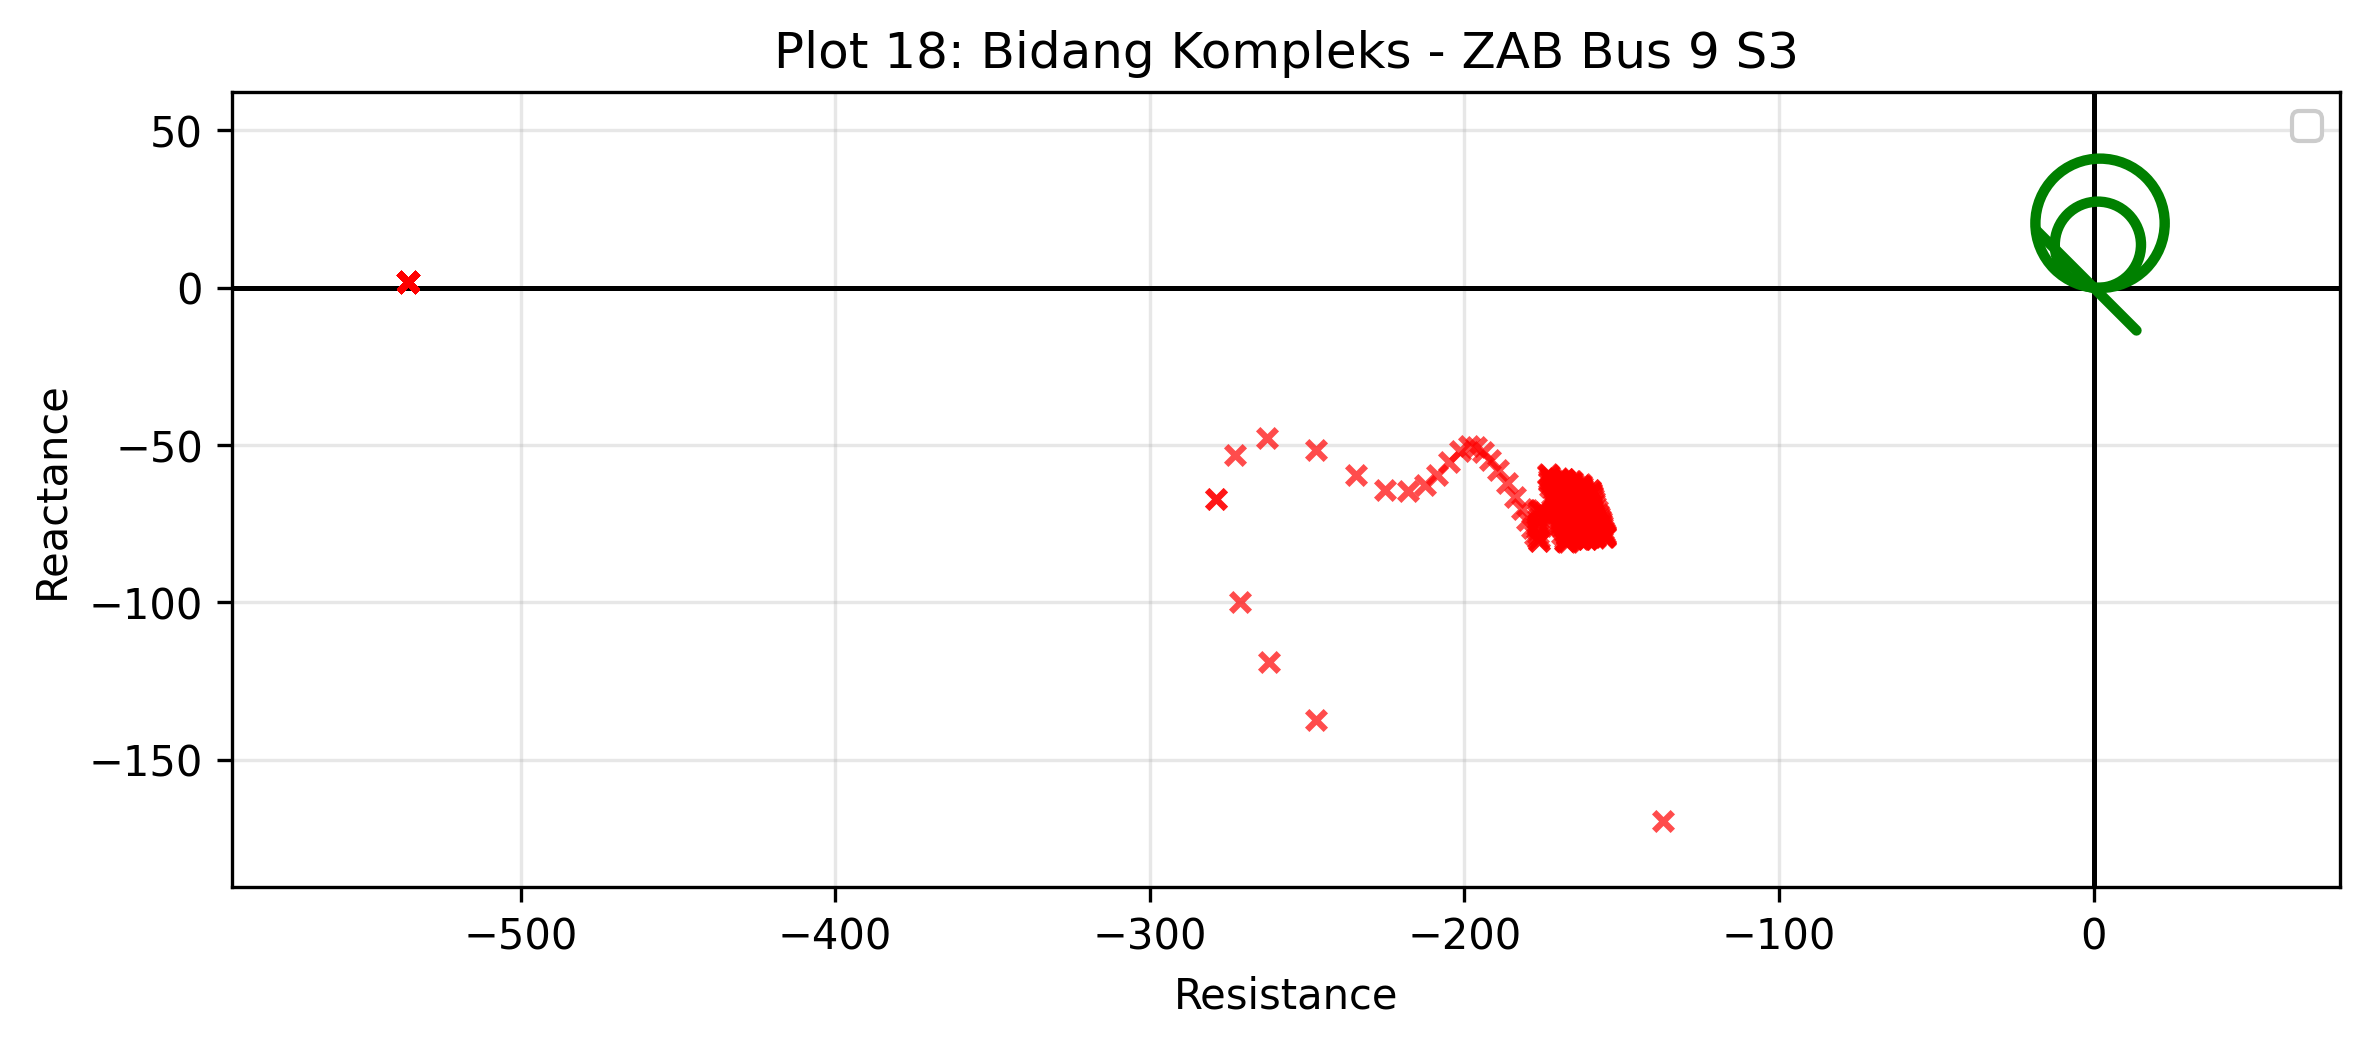
\includegraphics[width=\textwidth]{contents/chapter-4/PRIA_18_ZAB_Bus_9_S3.png}
        \caption{Seluruh Impedansi Tampak}
        \label{fig:PRIA_18_ZAB_Bus_9_S3}
    \end{subfigure}
    \hfill
    % Gambar sebelah kanan
    \begin{subfigure}[t]{0.48\textwidth}
        \centering
        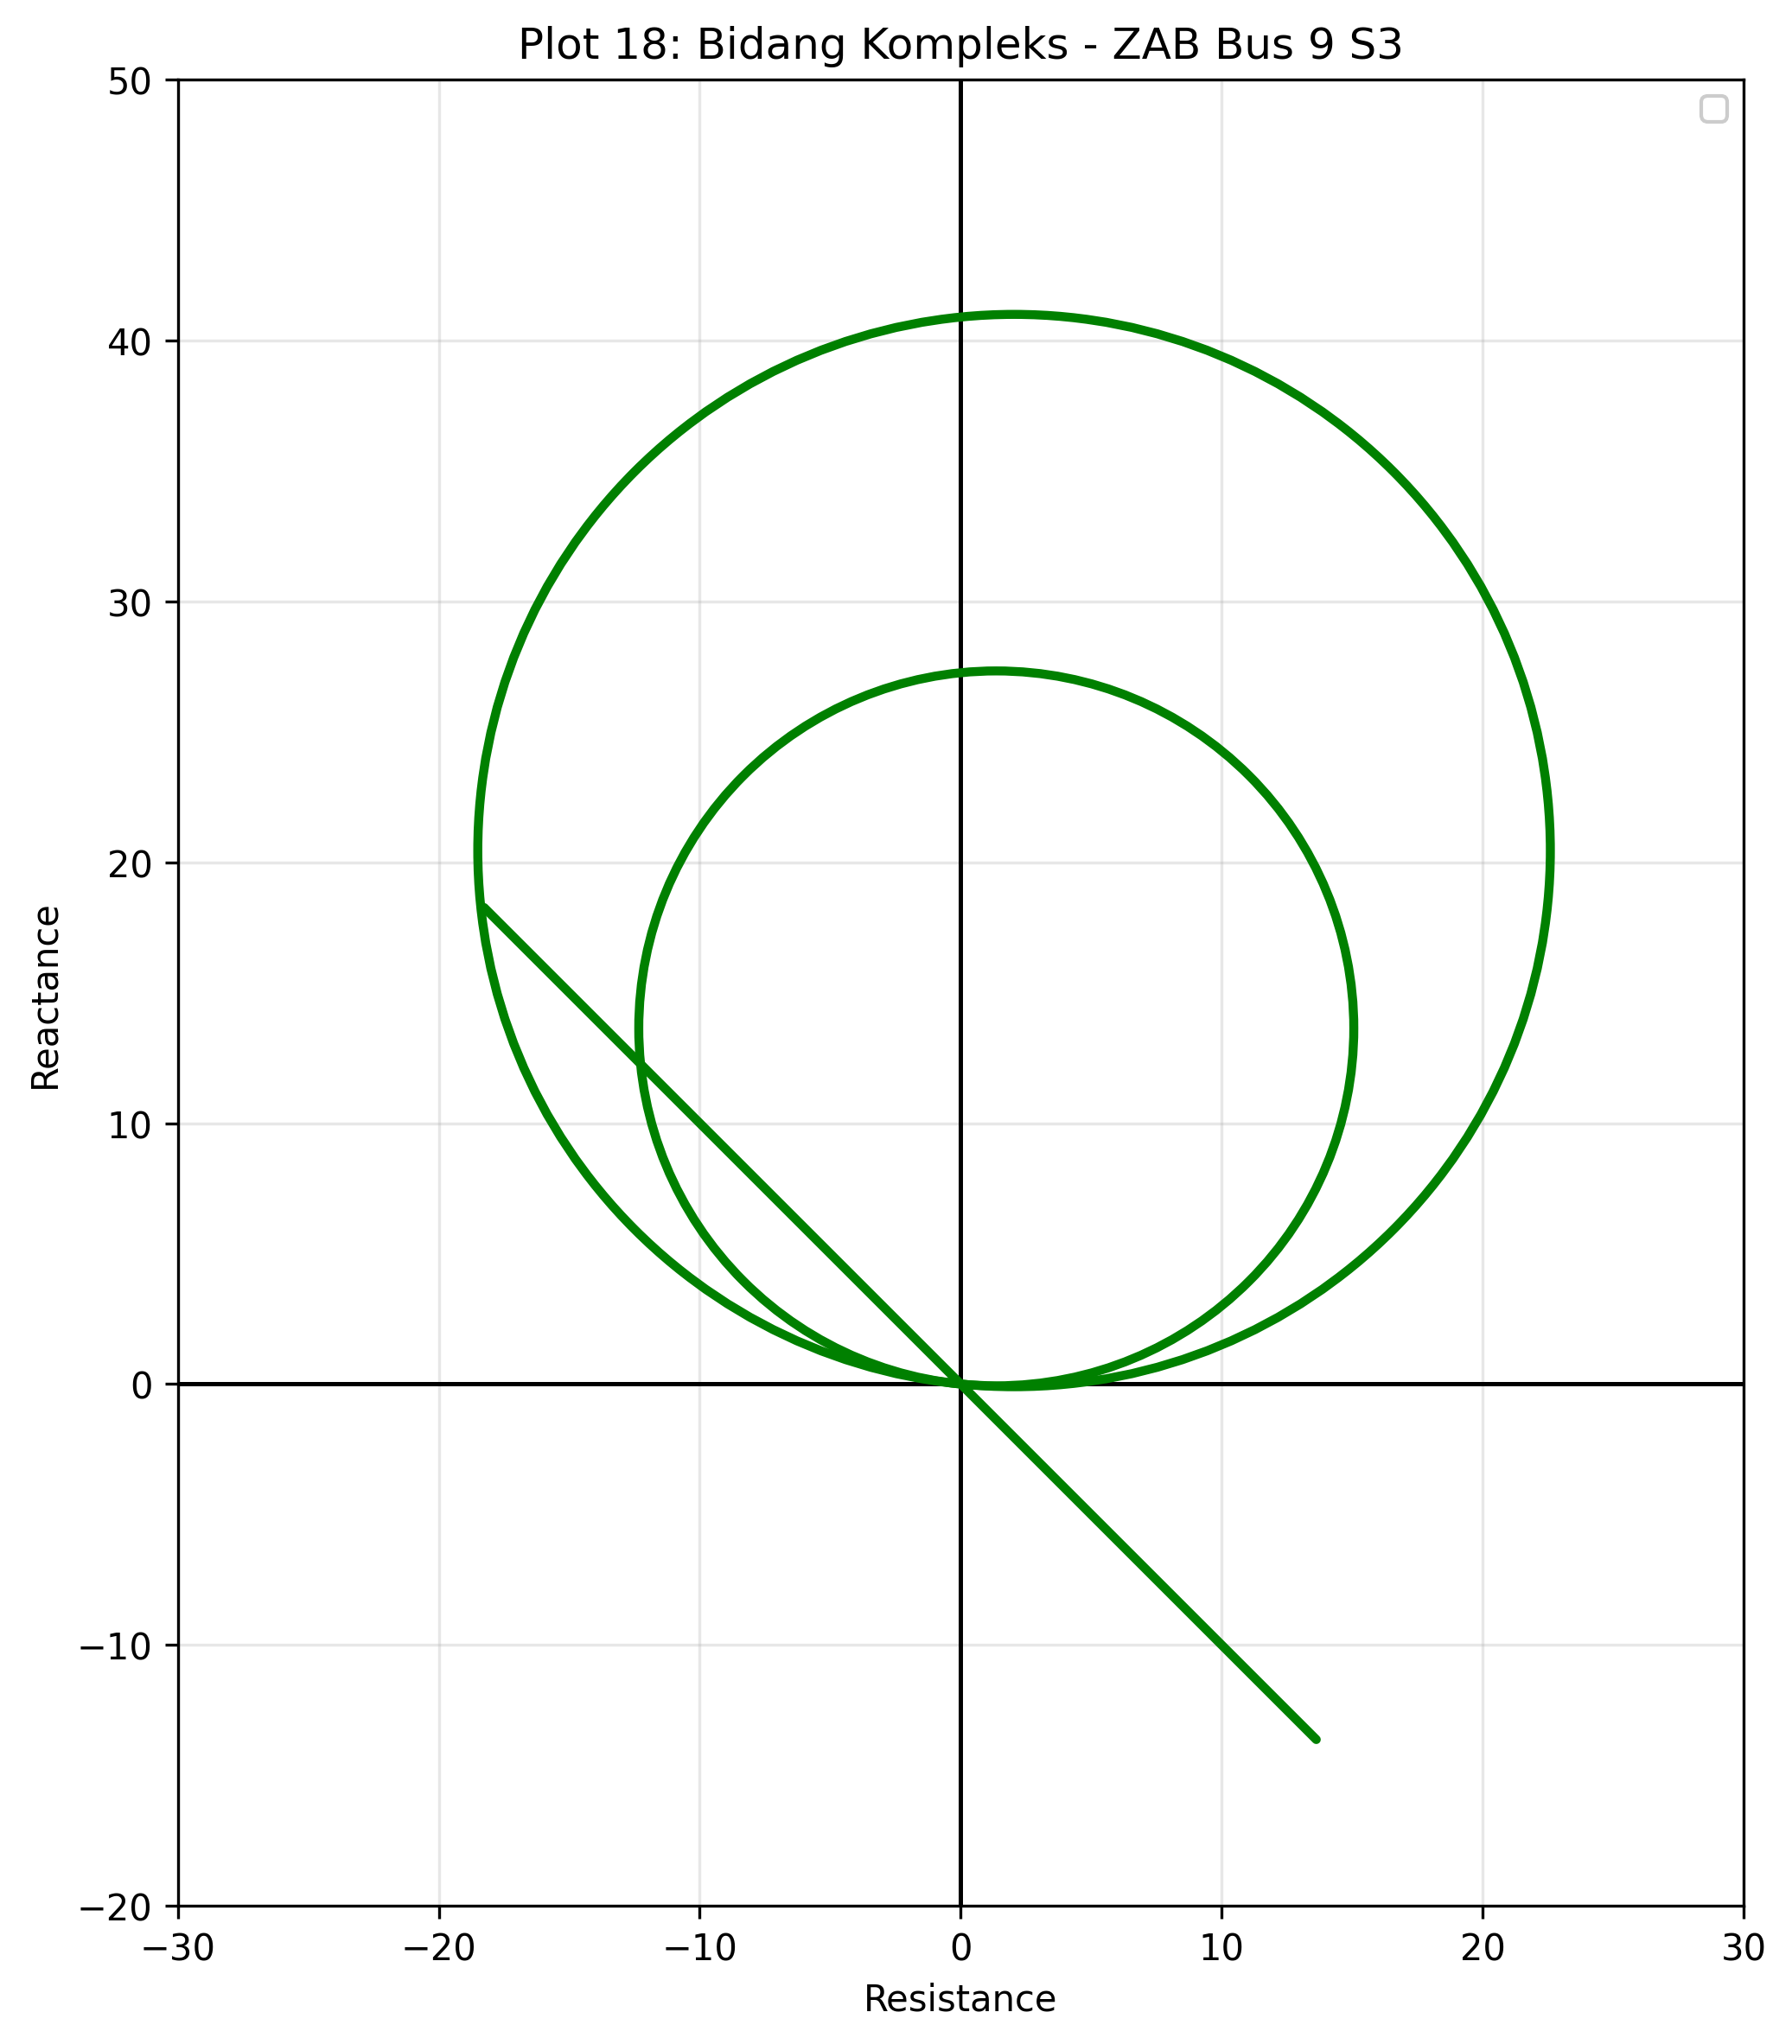
\includegraphics[width=\textwidth]{contents/chapter-4/PRIZI_18_ZAB_Bus_9_S3.png}
        \caption{Zoom In Pada Zona Proteksi}
        \label{fig:PRIZI_18_ZAB_Bus_9_S3}
    \end{subfigure}

    \caption{Impedansi Tampak ZAB Bus 9 Skenario 3}
    \label{fig:Impedansi_Tampak_ZAB_Bus_9_S3}
\end{figure}

Terlihat pada gambar \ref{fig:Impedansi_Tampak_ZAB_Bus_9_S3} bahwa impedansi tampak pada fasa A dengan fasa B yang dibaca oleh relay 21 sisi bus 9 saat terdapat gangguan bekerja dengan baik sesuai acuan pada \ref{subsec:tanpa_IBR_ex_dlg} relay 21 bus 9 tidak mendeteksi adanya gangguan sehingga tidak mengirimkan sinyal trip kepada CB.

%%%%%%%%%%%%%%%%%%%%%%%%%%%%%%%%%%%%%%%%%%%%%%%%%%%%%%%%%%%%%%%

% terlihat pada gambar \ref{fig:13_ZAG_Bus_8_S3_dengan_lingkaran_dan_garis} hingga \ref{fig:18_ZAB_Bus_9_S3_dengan_lingkaran_dan_garis} bahwa pada relay 21 sisi bus 8 mengalami over reach pada zona 1 serta mengalami drop out pada zona 2. untuk relay 21 pada sisi bus 9 bekerja normal sebagaimana mestinya.



\subsection{Skenario 4 : Wind Turbine Type 3 External 3P Fault}

Skenario ini digunakan untuk melihat respons relay 21 terhadap gangguan eksternal tiga fasa pada sistem dengan \textit{wind turbine type 3}. Gangguan tiga fasa memberikan kondisi pembanding terhadap gangguan tak seimbang karena pembacaan relay lebih dominan dikaitkan dengan elemen fasa-fasa dan komponen urutan positif.

Dekomposisi komponen urutan arus pada Gambar \ref{fig:decomposition_sequence_current_s4} membantu menjelaskan karakter arus yang diterima TL89 sebelum respons relay dianalisis. Dengan konteks tersebut, pembahasan berikutnya difokuskan pada elemen ZAB, ZBC, dan ZCA untuk menilai apakah relay 21 tetap menahan operasi pada gangguan eksternal atau menunjukkan penyimpangan terhadap acuan kondisi dasar.

% \begin{figure}[H]
%     \centering
%     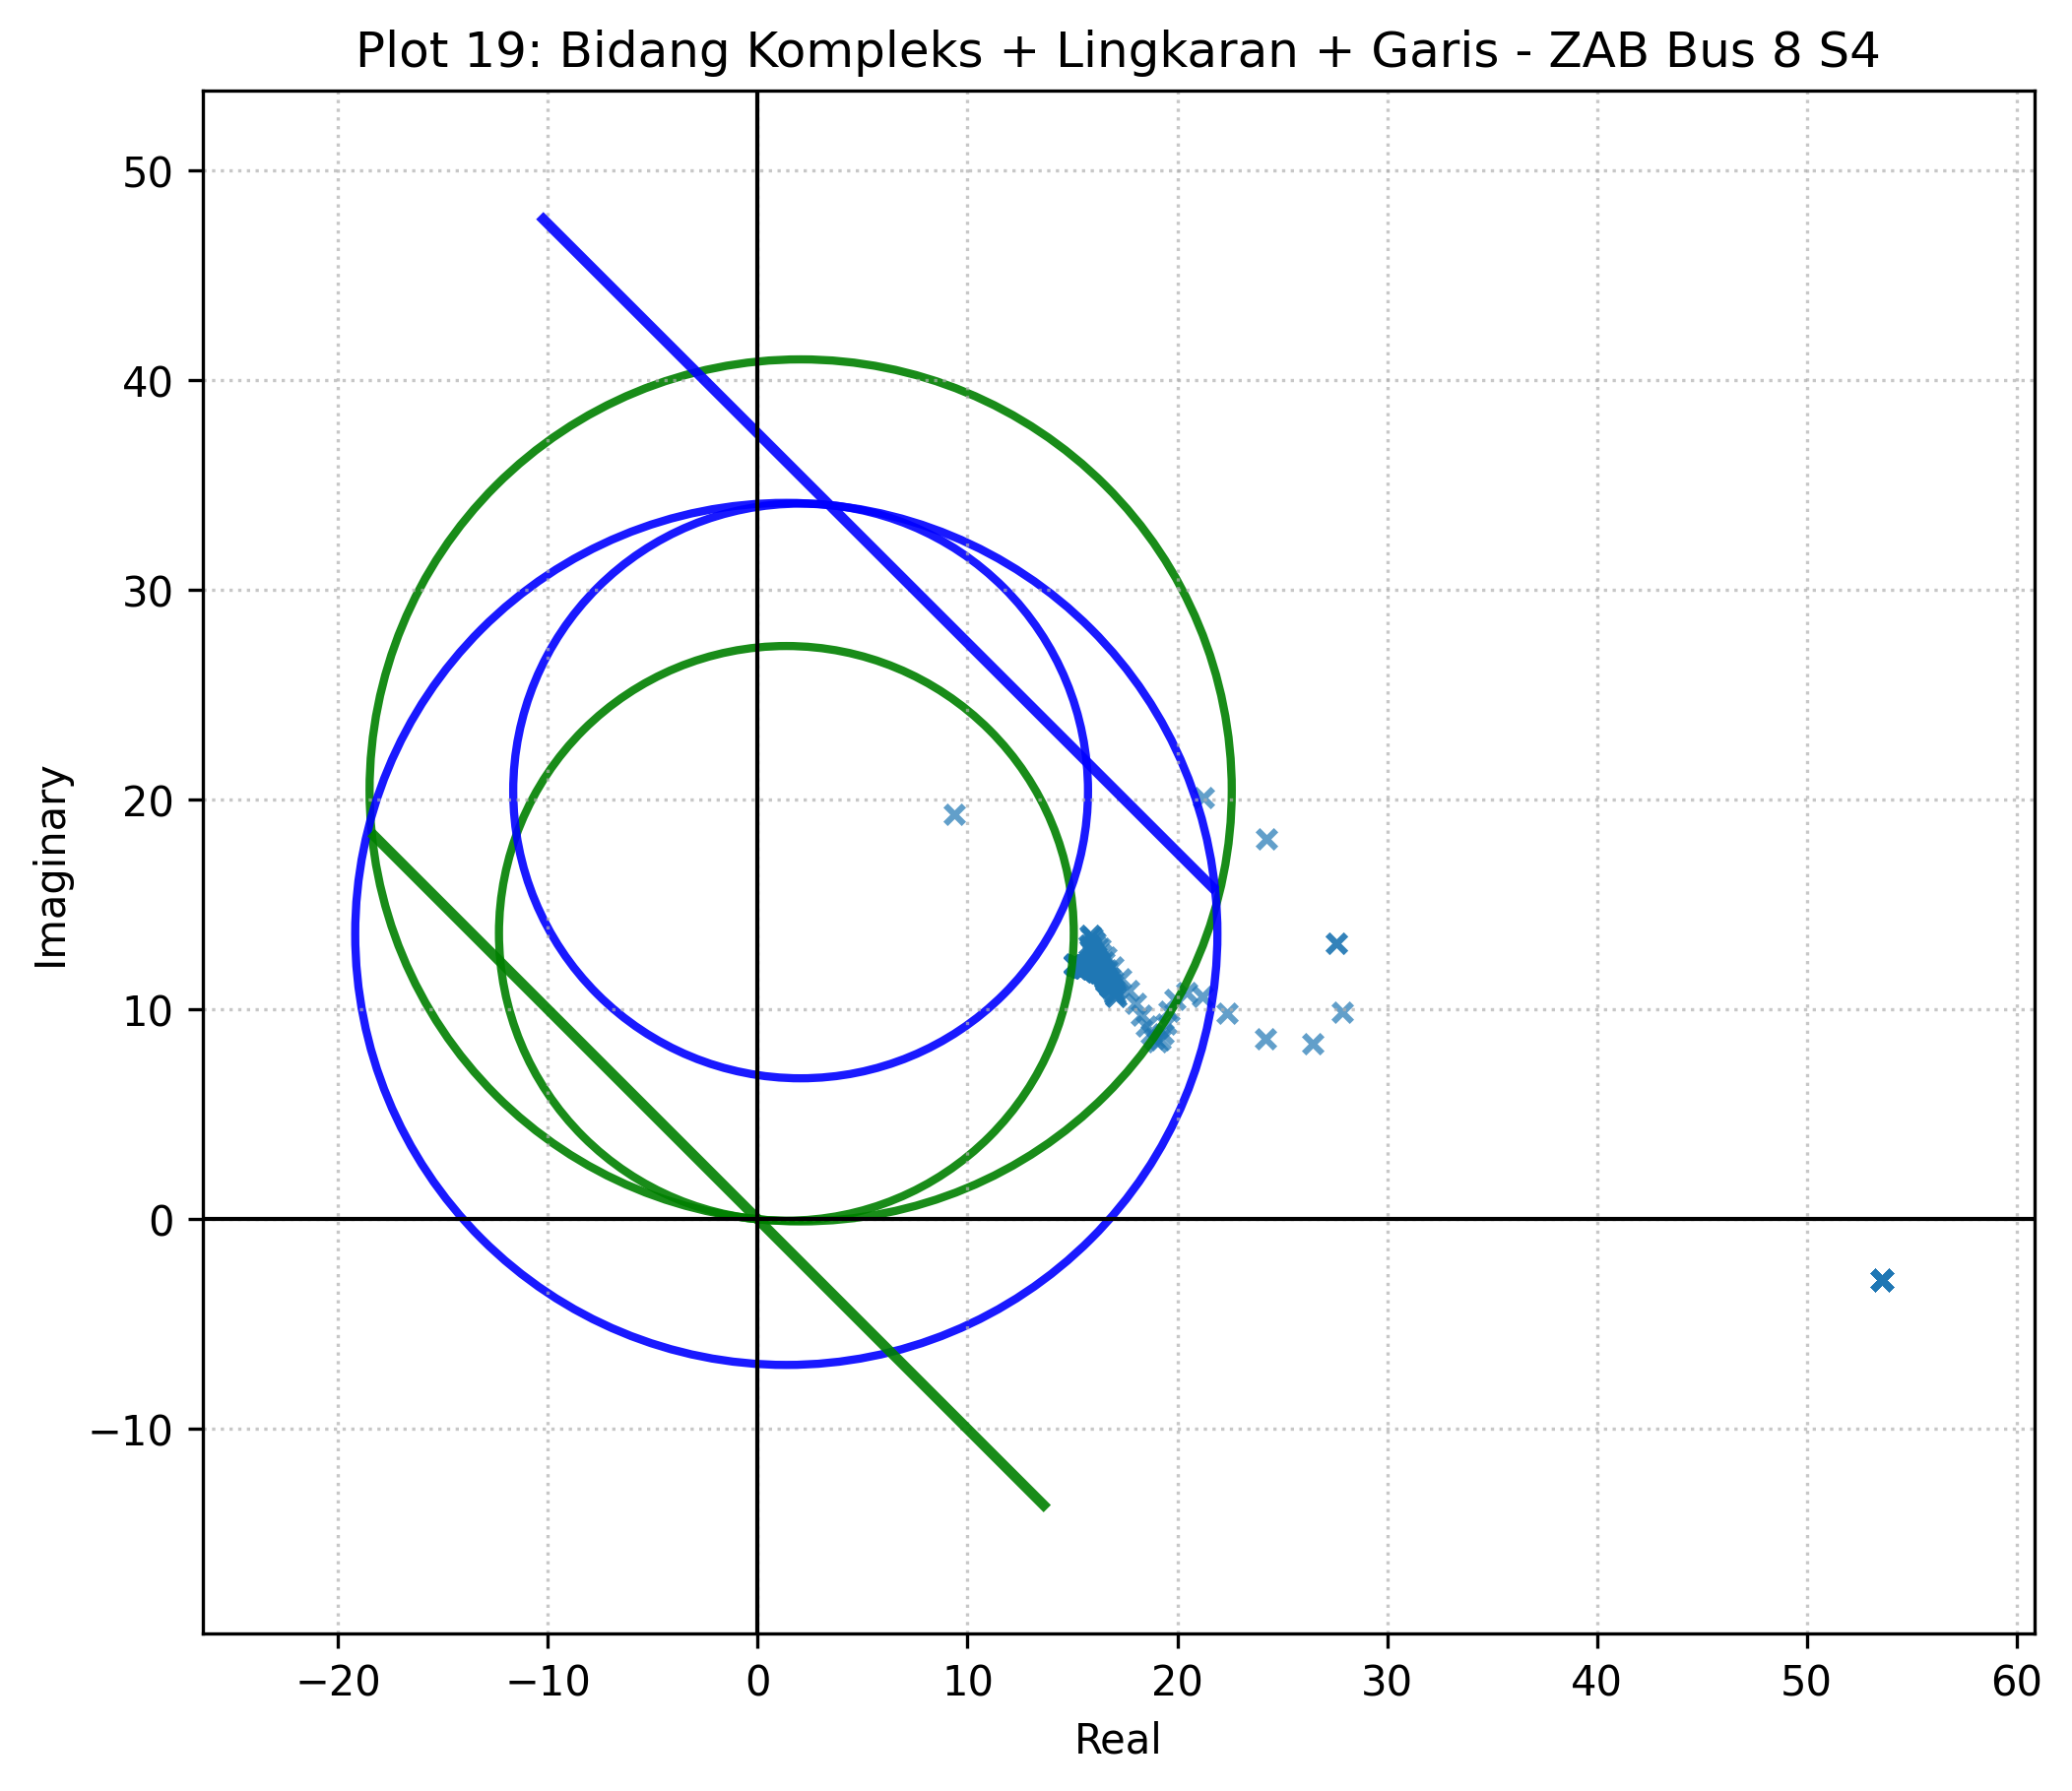
\includegraphics[width=0.8\textwidth]{contents/chapter-4/19_ZAB_Bus_8_S4_dengan_lingkaran_dan_garis.png}
%     \caption{Impedansi Tampak ZAB Bus 8 Skenario 4}
%     \label{fig:19_ZAB_Bus_8_S4_dengan_lingkaran_dan_garis}
% \end{figure}

% Terlihat pada gambar \ref{fig:19_ZAB_Bus_8_S4_dengan_lingkaran_dan_garis} bahwa impedansi tampak pada fasa A dengan fasa B yang dibaca oleh relay 21 sisi bus 8 saat terdapat gangguan mengalami over reach pada zona 1 serta mengalami drop out pada zona 2 sehingga dengan acuan pada \ref{subsec:tanpa_IBR_ex_3p} relay 21 bus 8 mengalami missoperation trip pada zona 1.

%%%%%%%%%%%%%%%%%%%%%%%%%%%%%%%%%SISI PRIMER%%%%%%%%%%%%%%%%%%%%%%%%%%%%%%%%%%

\begin{figure}[H]
    \centering
    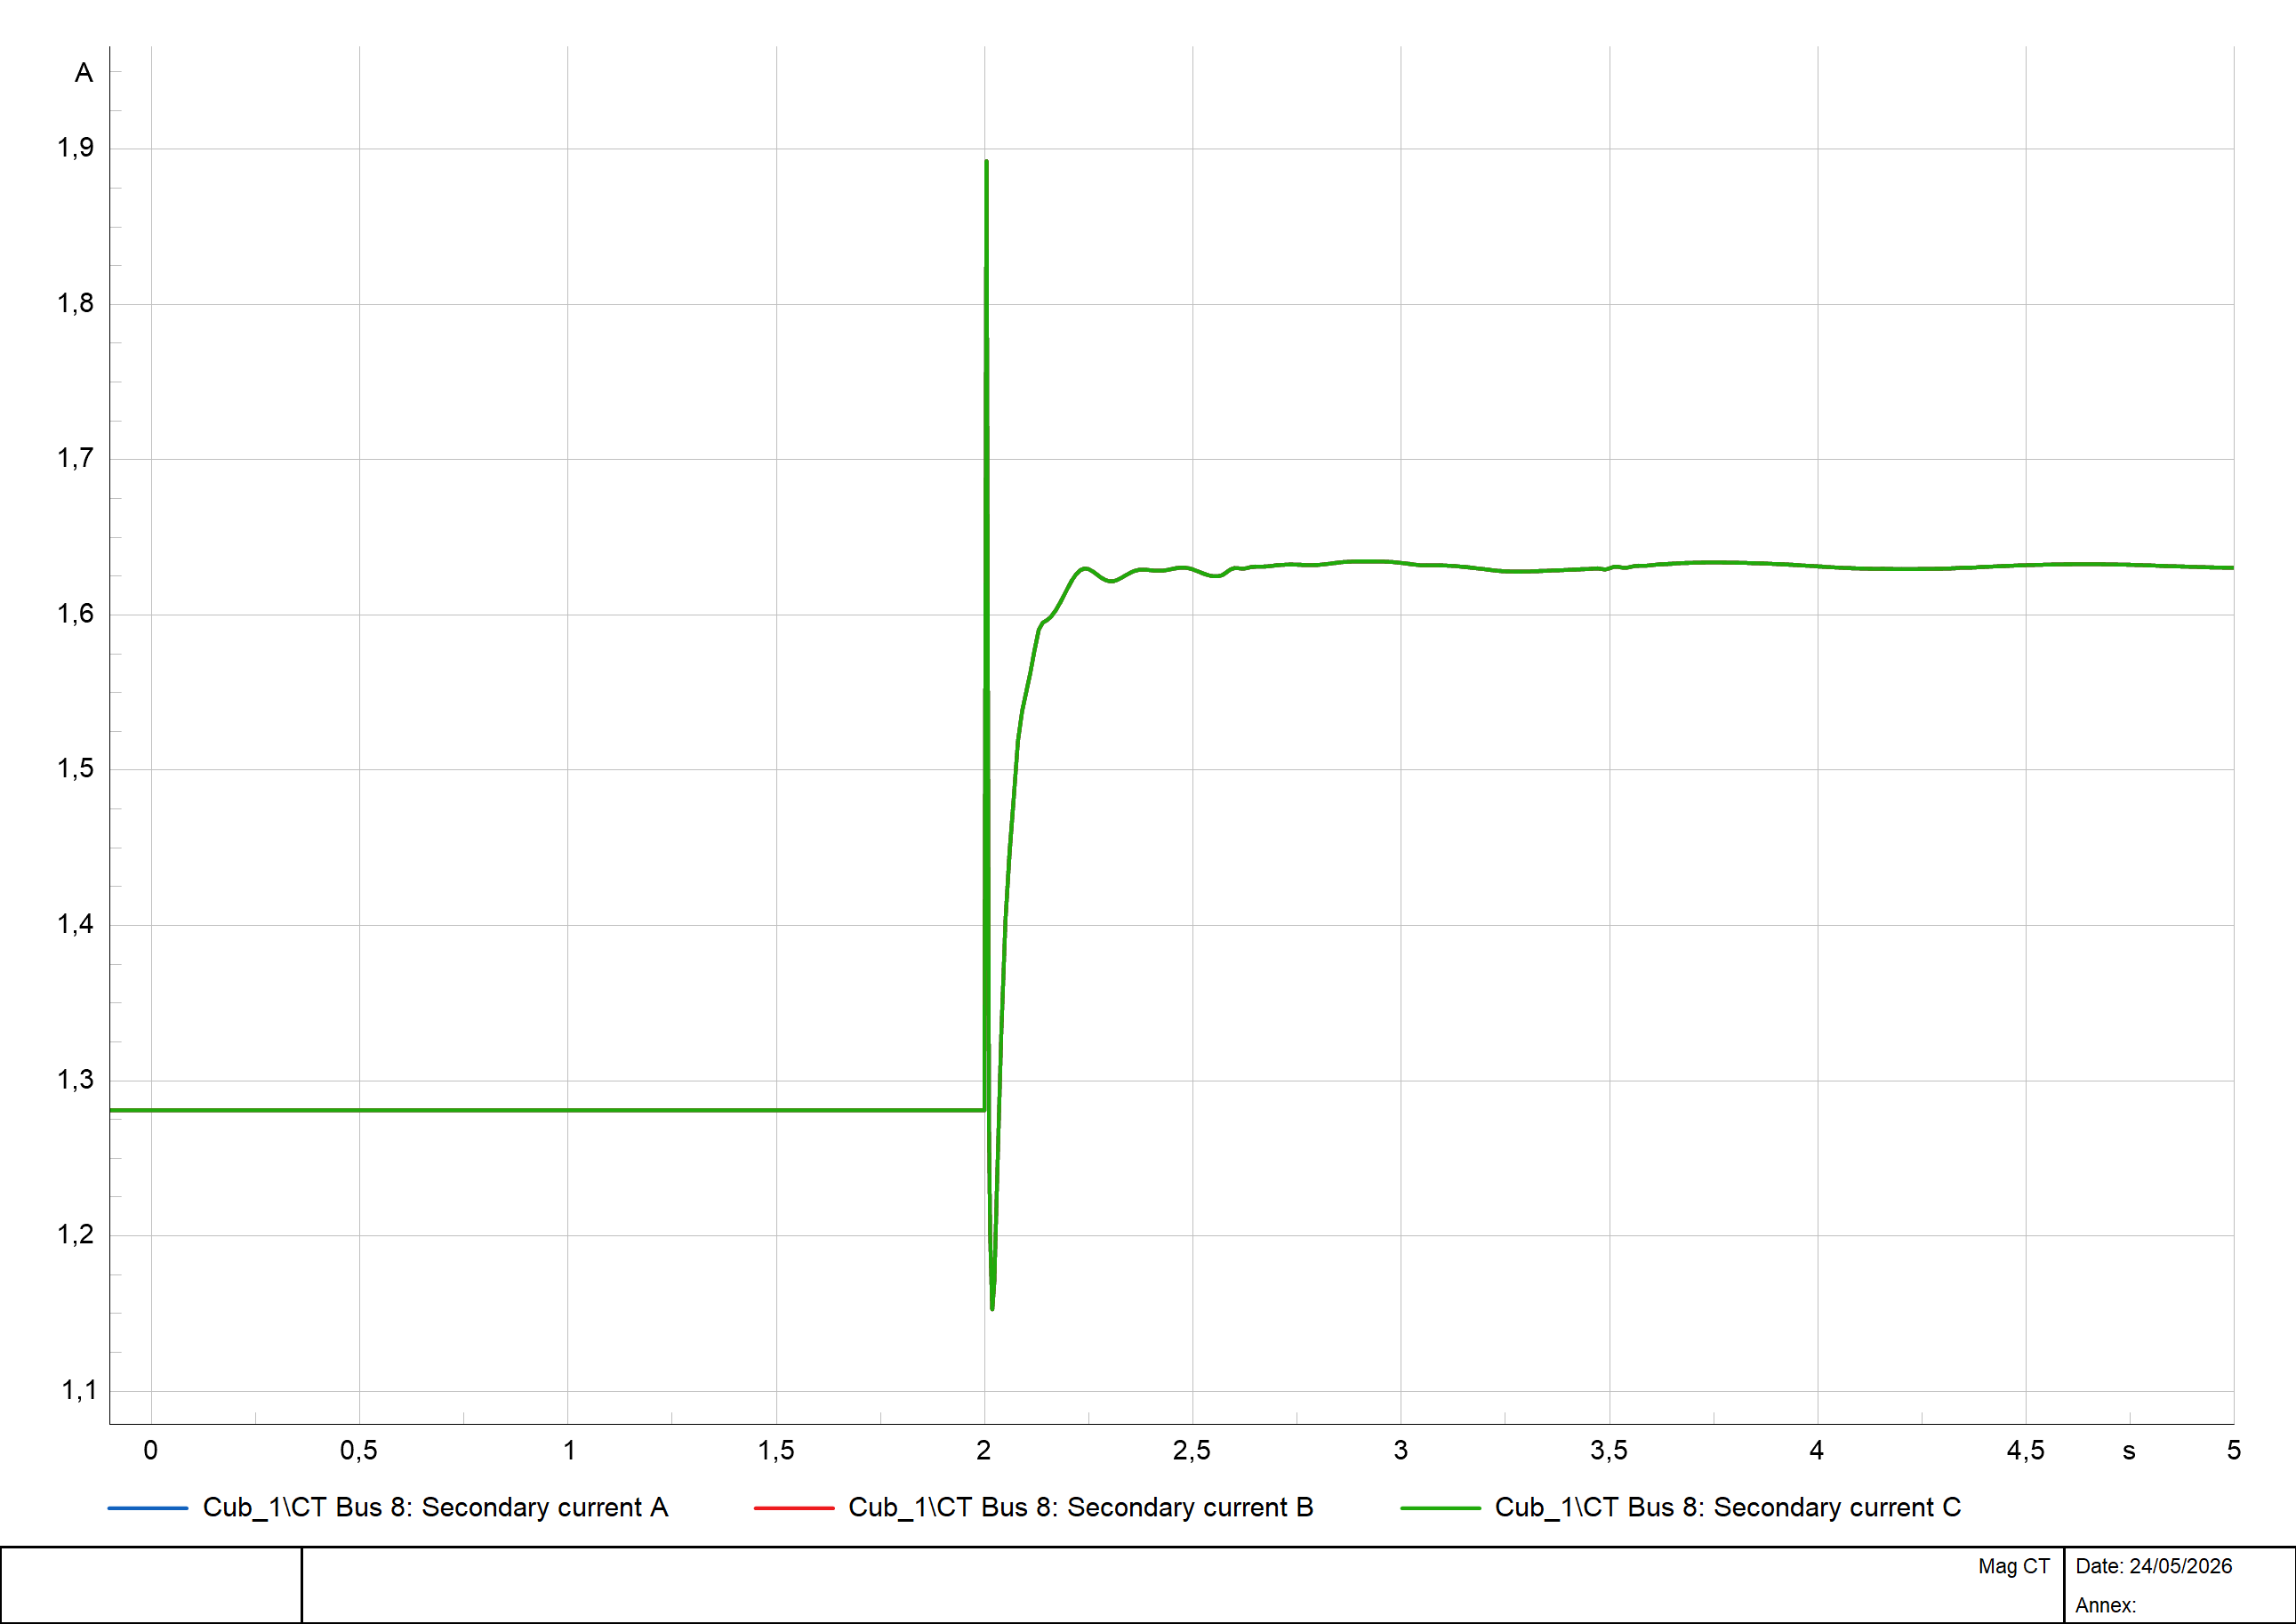
\includegraphics[width=0.8\textwidth]{contents/chapter-4/Bus_8_Ex_3P_S4.png}
    \caption{Arus Sekunder CT Bus 8 Skenario 4}
    \label{fig:Bus_8_Ex_3P_S4}
\end{figure}

Gambar \ref{fig:Bus_8_Ex_3P_S4} menunjukkan arus sekunder CT pada Bus 8 untuk skenario 4. Sebelum gangguan, arus pada ketiga fasa berada pada nilai 1,281 A sekunder. Setelah gangguan tiga fasa terjadi, arus pada ketiga fasa meningkat menjadi 1,892 A sekunder atau 1,48 p.u. Kenaikan arus tersebut menunjukkan adanya perubahan arus saat gangguan, tetapi nilainya masih belum memenuhi arus minimum yang diperlukan untuk membuat relay 21 sisi Bus 8 aktif.

\begin{figure}[H]
    \centering

    % Gambar sebelah kiri
    \begin{subfigure}[t]{0.48\textwidth}
        \centering
        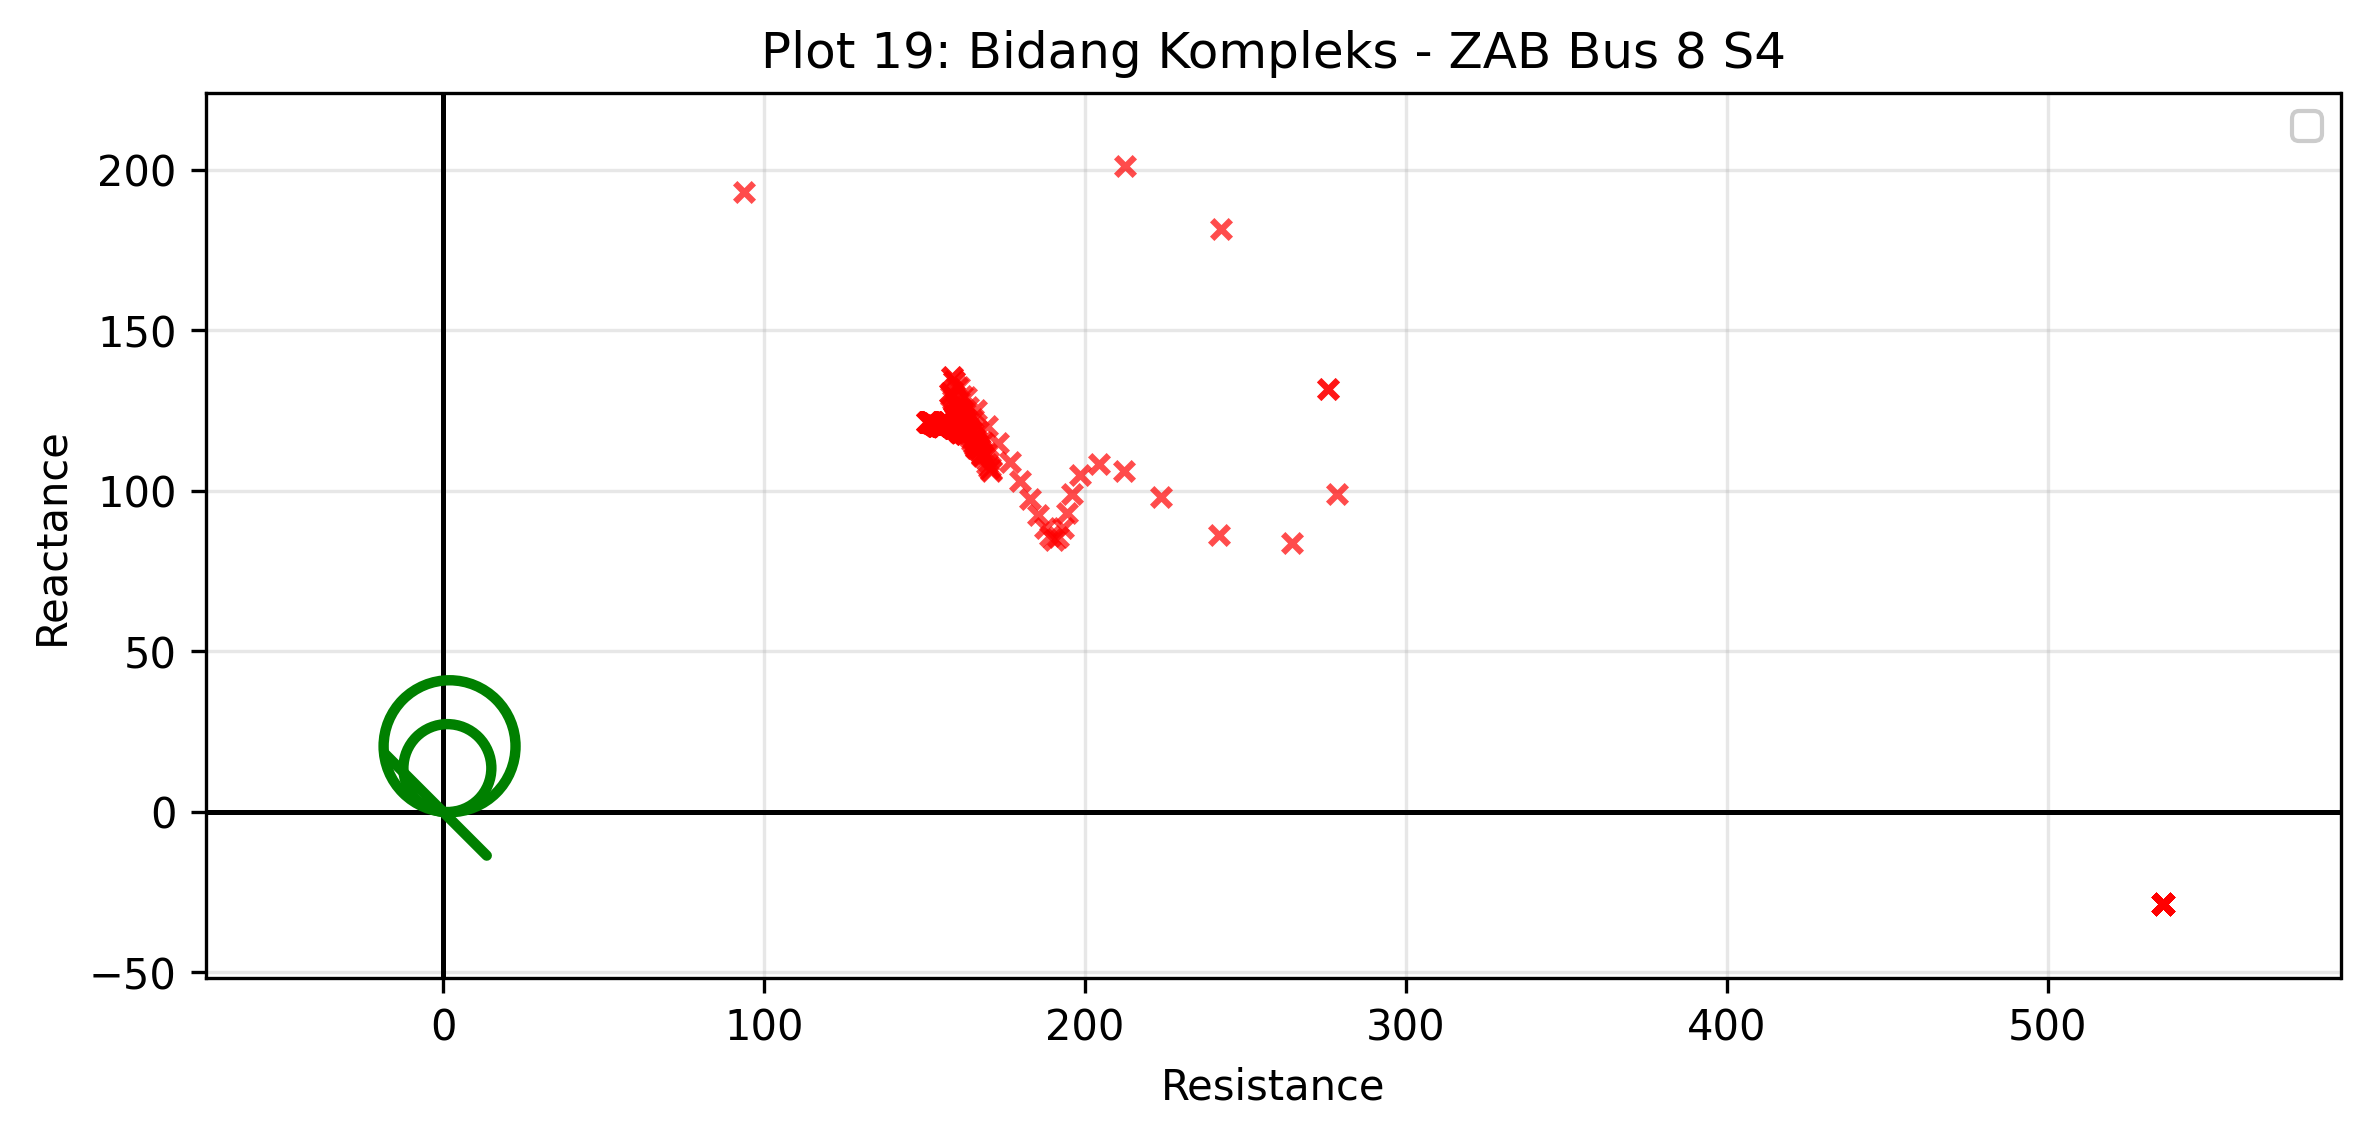
\includegraphics[width=\textwidth]{contents/chapter-4/PRIA_19_ZAB_Bus_8_S4.png}
        \caption{Seluruh Impedansi Tampak}
        \label{fig:PRIA_19_ZAB_Bus_8_S4}
    \end{subfigure}
    \hfill
    % Gambar sebelah kanan
    \begin{subfigure}[t]{0.48\textwidth}
        \centering
        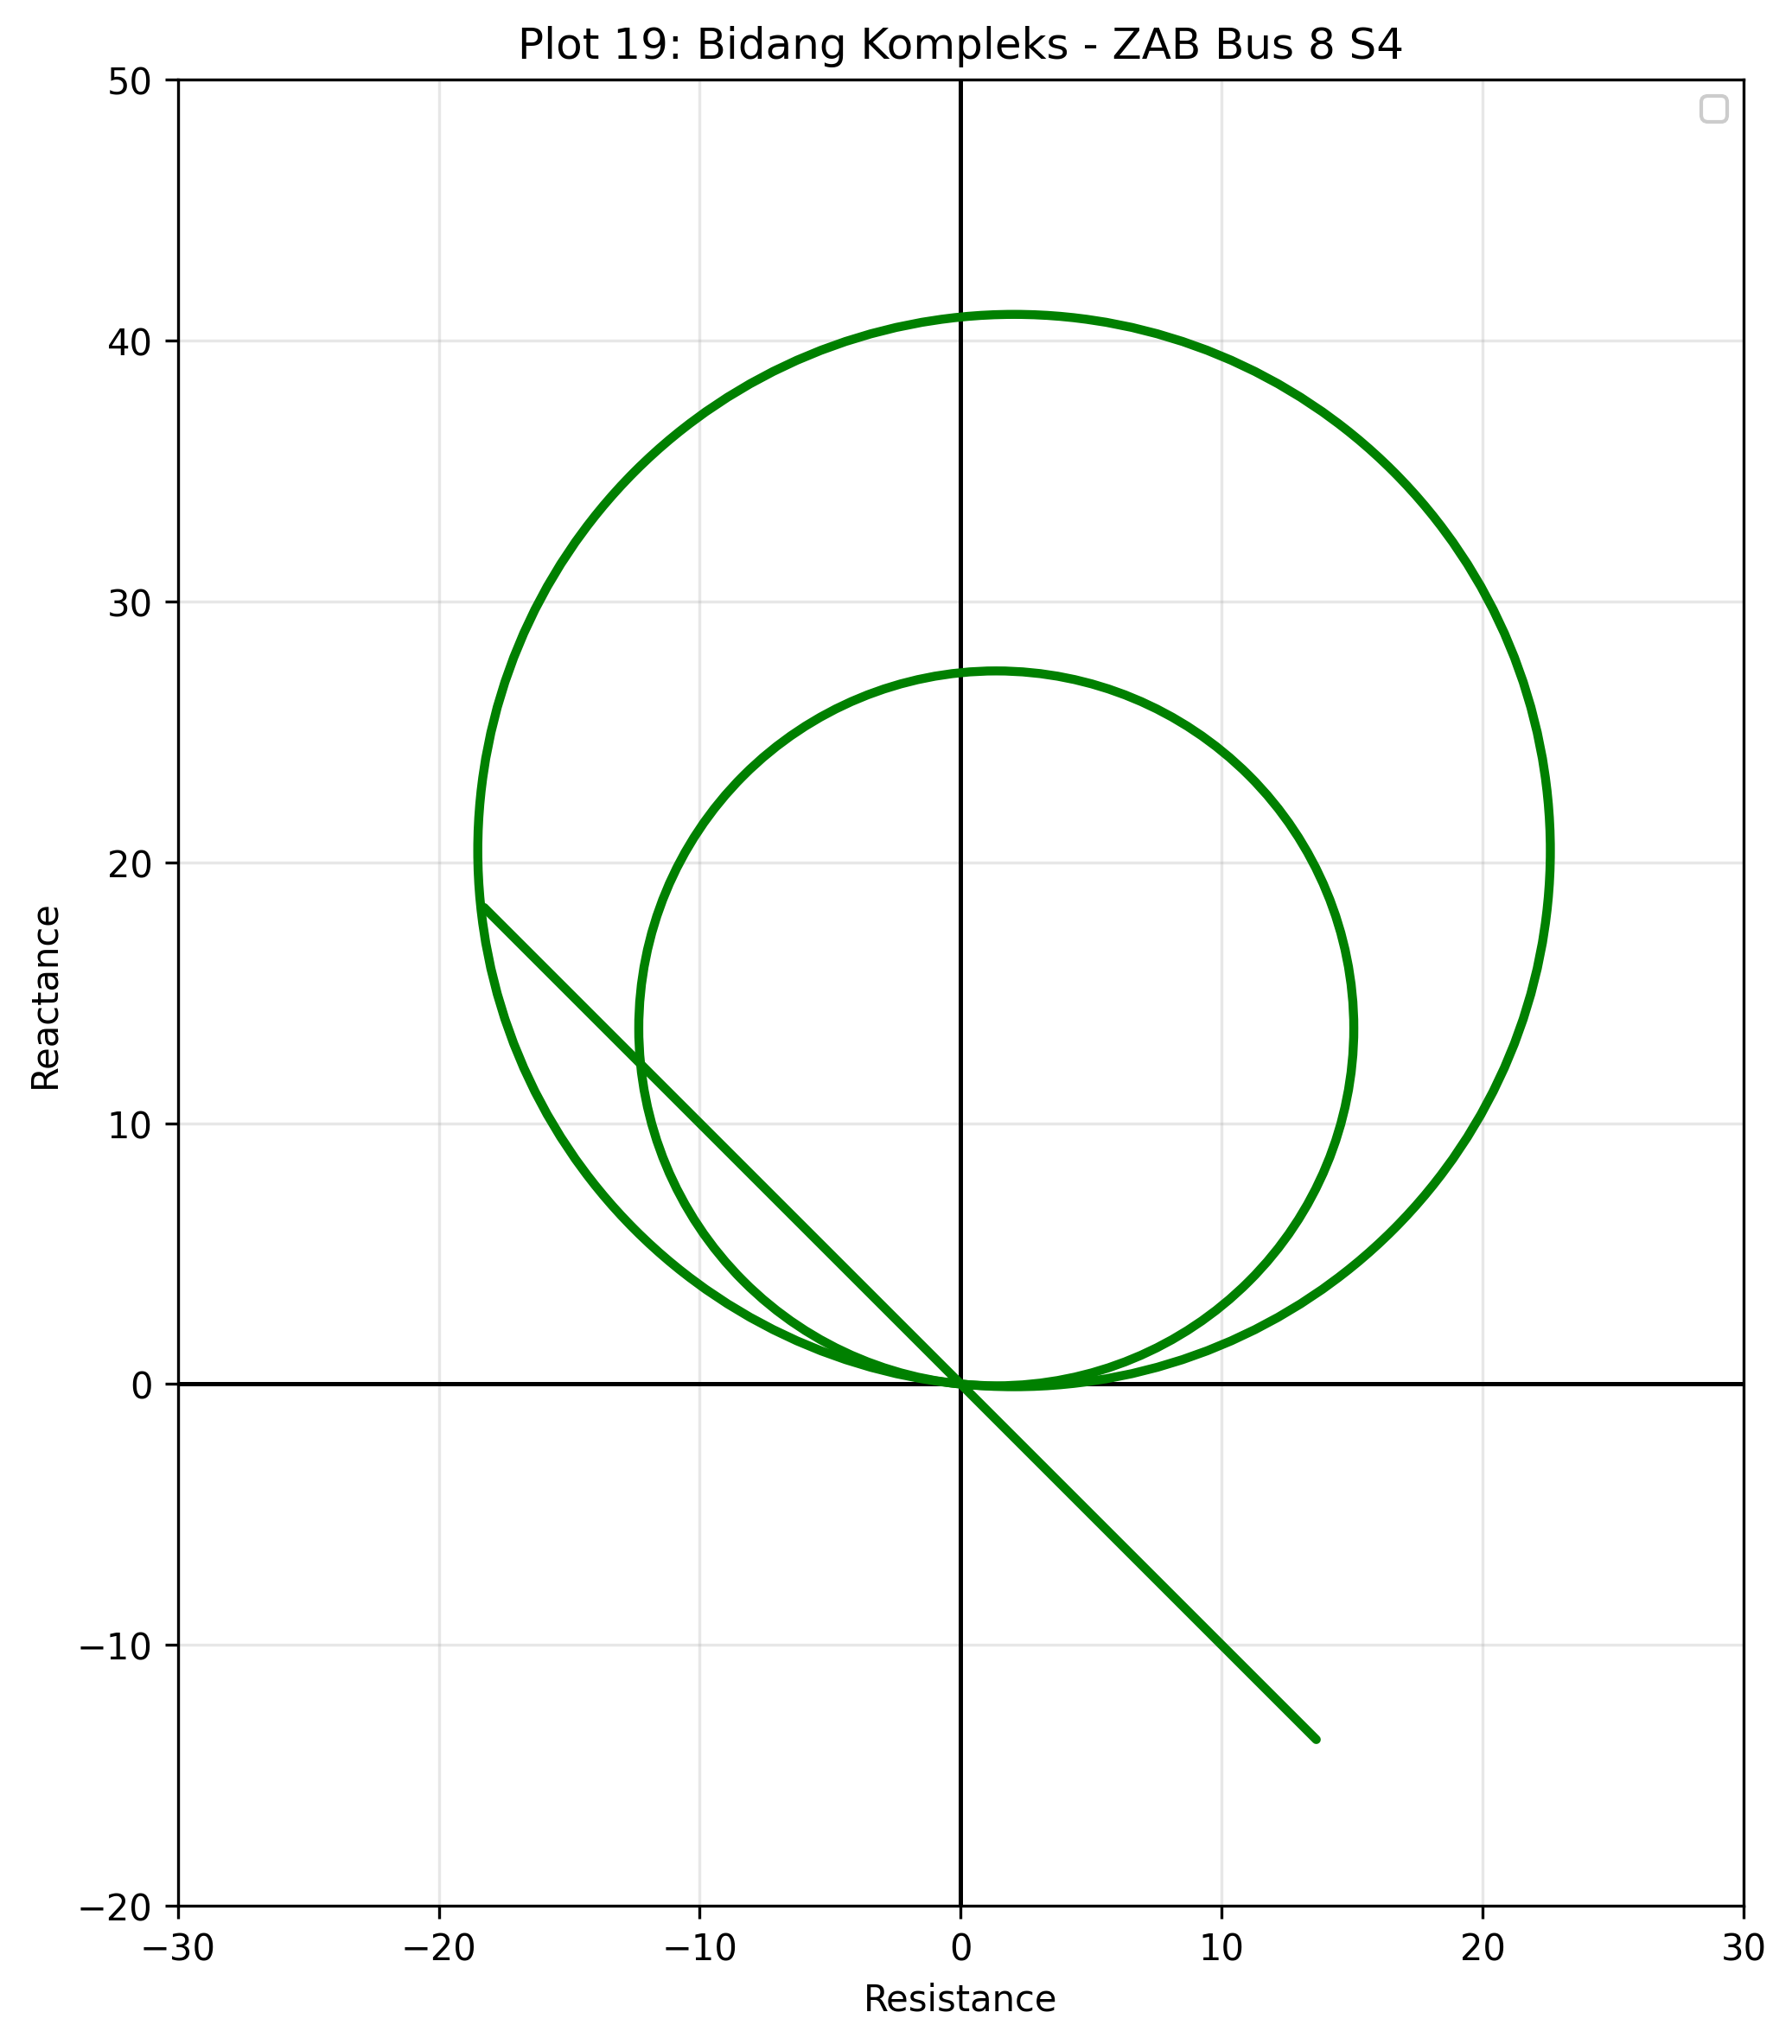
\includegraphics[width=\textwidth]{contents/chapter-4/PRIZI_19_ZAB_Bus_8_S4.png}
        \caption{Zoom In Pada Zona Proteksi}
        \label{fig:PRIZI_19_ZAB_Bus_8_S4}
    \end{subfigure}

    \caption{Impedansi Tampak ZAB Bus 8 Skenario 4}
    \label{fig:Impedansi_Tampak_ZAB_Bus_8_S4}
\end{figure}

Gambar \ref{fig:Impedansi_Tampak_ZAB_Bus_8_S4} menunjukkan bahwa impedansi tampak loop fasa A dengan fasa B yang dibaca oleh relay 21 sisi Bus 8 tidak masuk ke dalam zona proteksi. Kondisi ini sejalan dengan pembacaan arus sekunder CT pada Gambar \ref{fig:Bus_8_Ex_3P_S4}, karena arus gangguan yang terbaca masih belum memenuhi syarat \textit{starting} untuk membuat relay aktif. Dengan mengacu pada kondisi dasar gangguan eksternal tiga fasa pada Subbab \ref{subsec:tanpa_IBR_ex_3p}, respons relay 21 sisi Bus 8 pada elemen ini dikategorikan mengalami \textit{misoperation}.

%%%%%%%%%%%%%%%%%%%%%%%%%%%%%%%%%%%%%%%%%%%%%%%%%%%%%%%%%%%%%%%

% \begin{figure}[H]
%     \centering
%     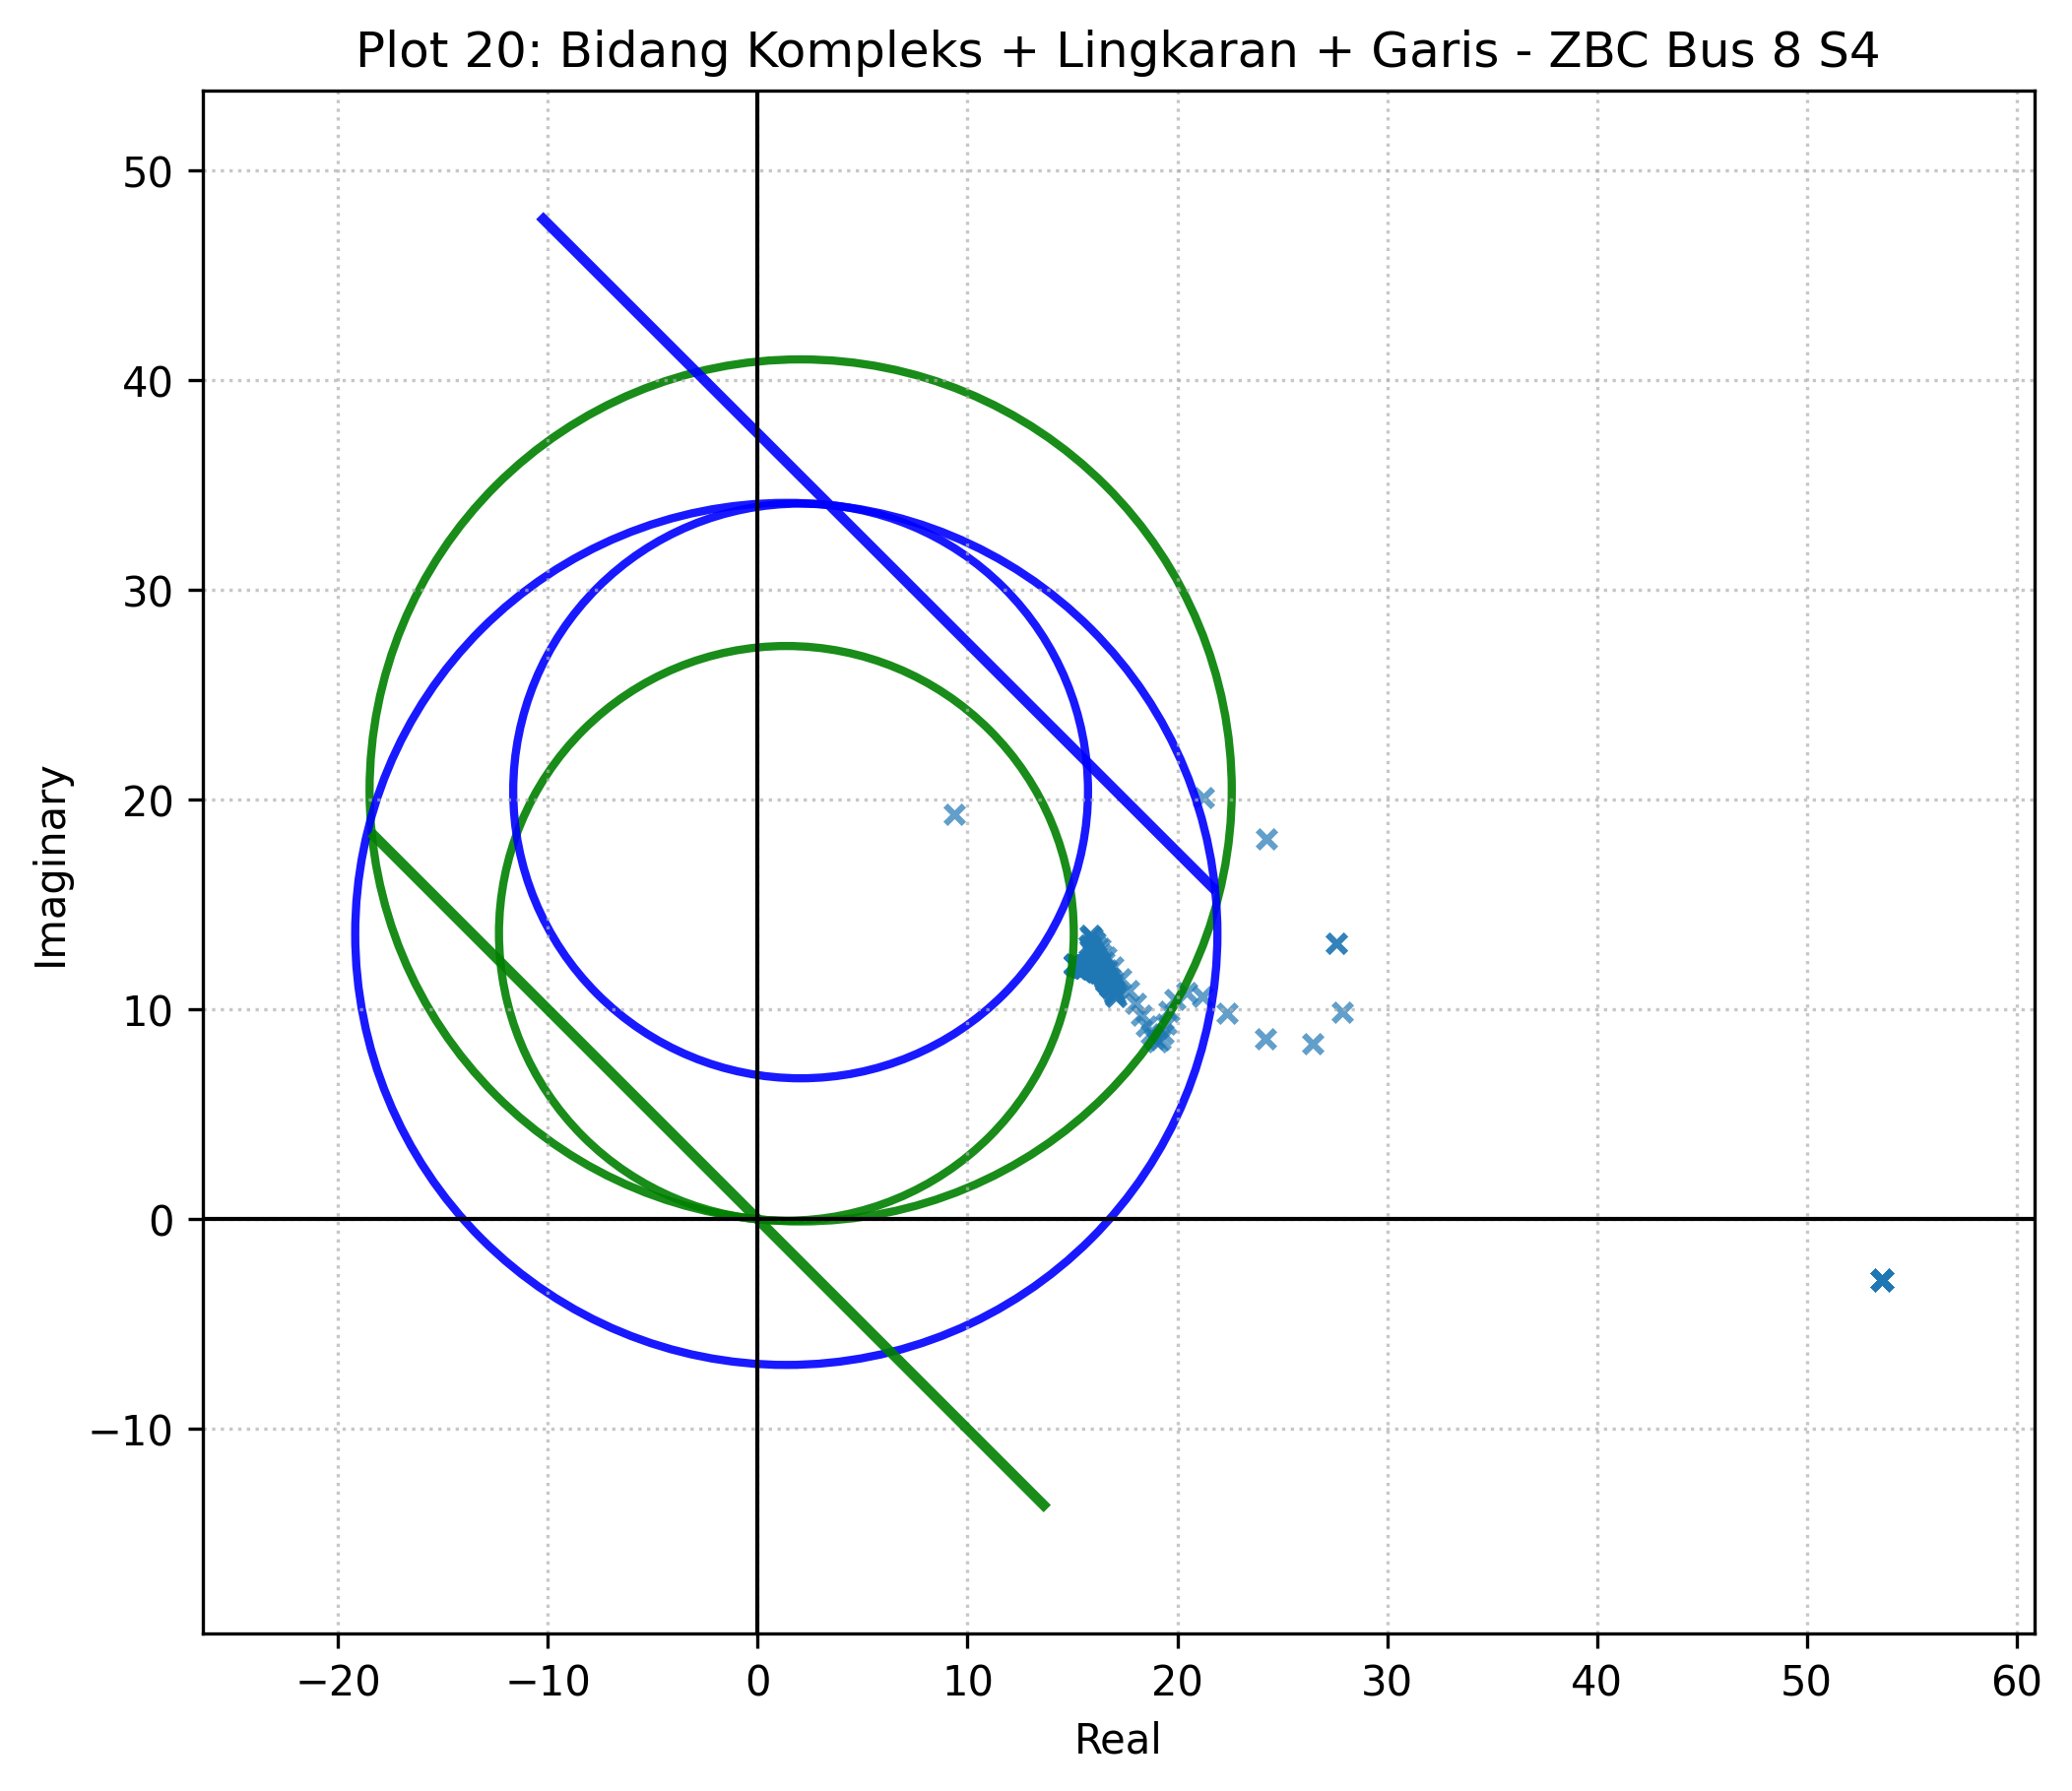
\includegraphics[width=0.8\textwidth]{contents/chapter-4/20_ZBC_Bus_8_S4_dengan_lingkaran_dan_garis.png}
%     \caption{Impedansi Tampak ZBC Bus 8 Skenario 4}
%     \label{fig:20_ZBC_Bus_8_S4_dengan_lingkaran_dan_garis}
% \end{figure}

% Terlihat pada gambar \ref{fig:20_ZBC_Bus_8_S4_dengan_lingkaran_dan_garis} bahwa impedansi tampak pada fasa B dengan fasa C yang dibaca oleh relay 21 sisi bus 8 saat terdapat gangguan mengalami over reach pada zona 1 serta mengalami drop out pada zona 2 sehingga dengan acuan pada \ref{subsec:tanpa_IBR_ex_3p} relay 21 bus 8 mengalami missoperation trip pada zona 1.

%%%%%%%%%%%%%%%%%%%%%%%%%%%%%%%%%SISI PRIMER%%%%%%%%%%%%%%%%%%%%%%%%%%%%%%%%%%

% \begin{figure}[H]
%     \centering
%     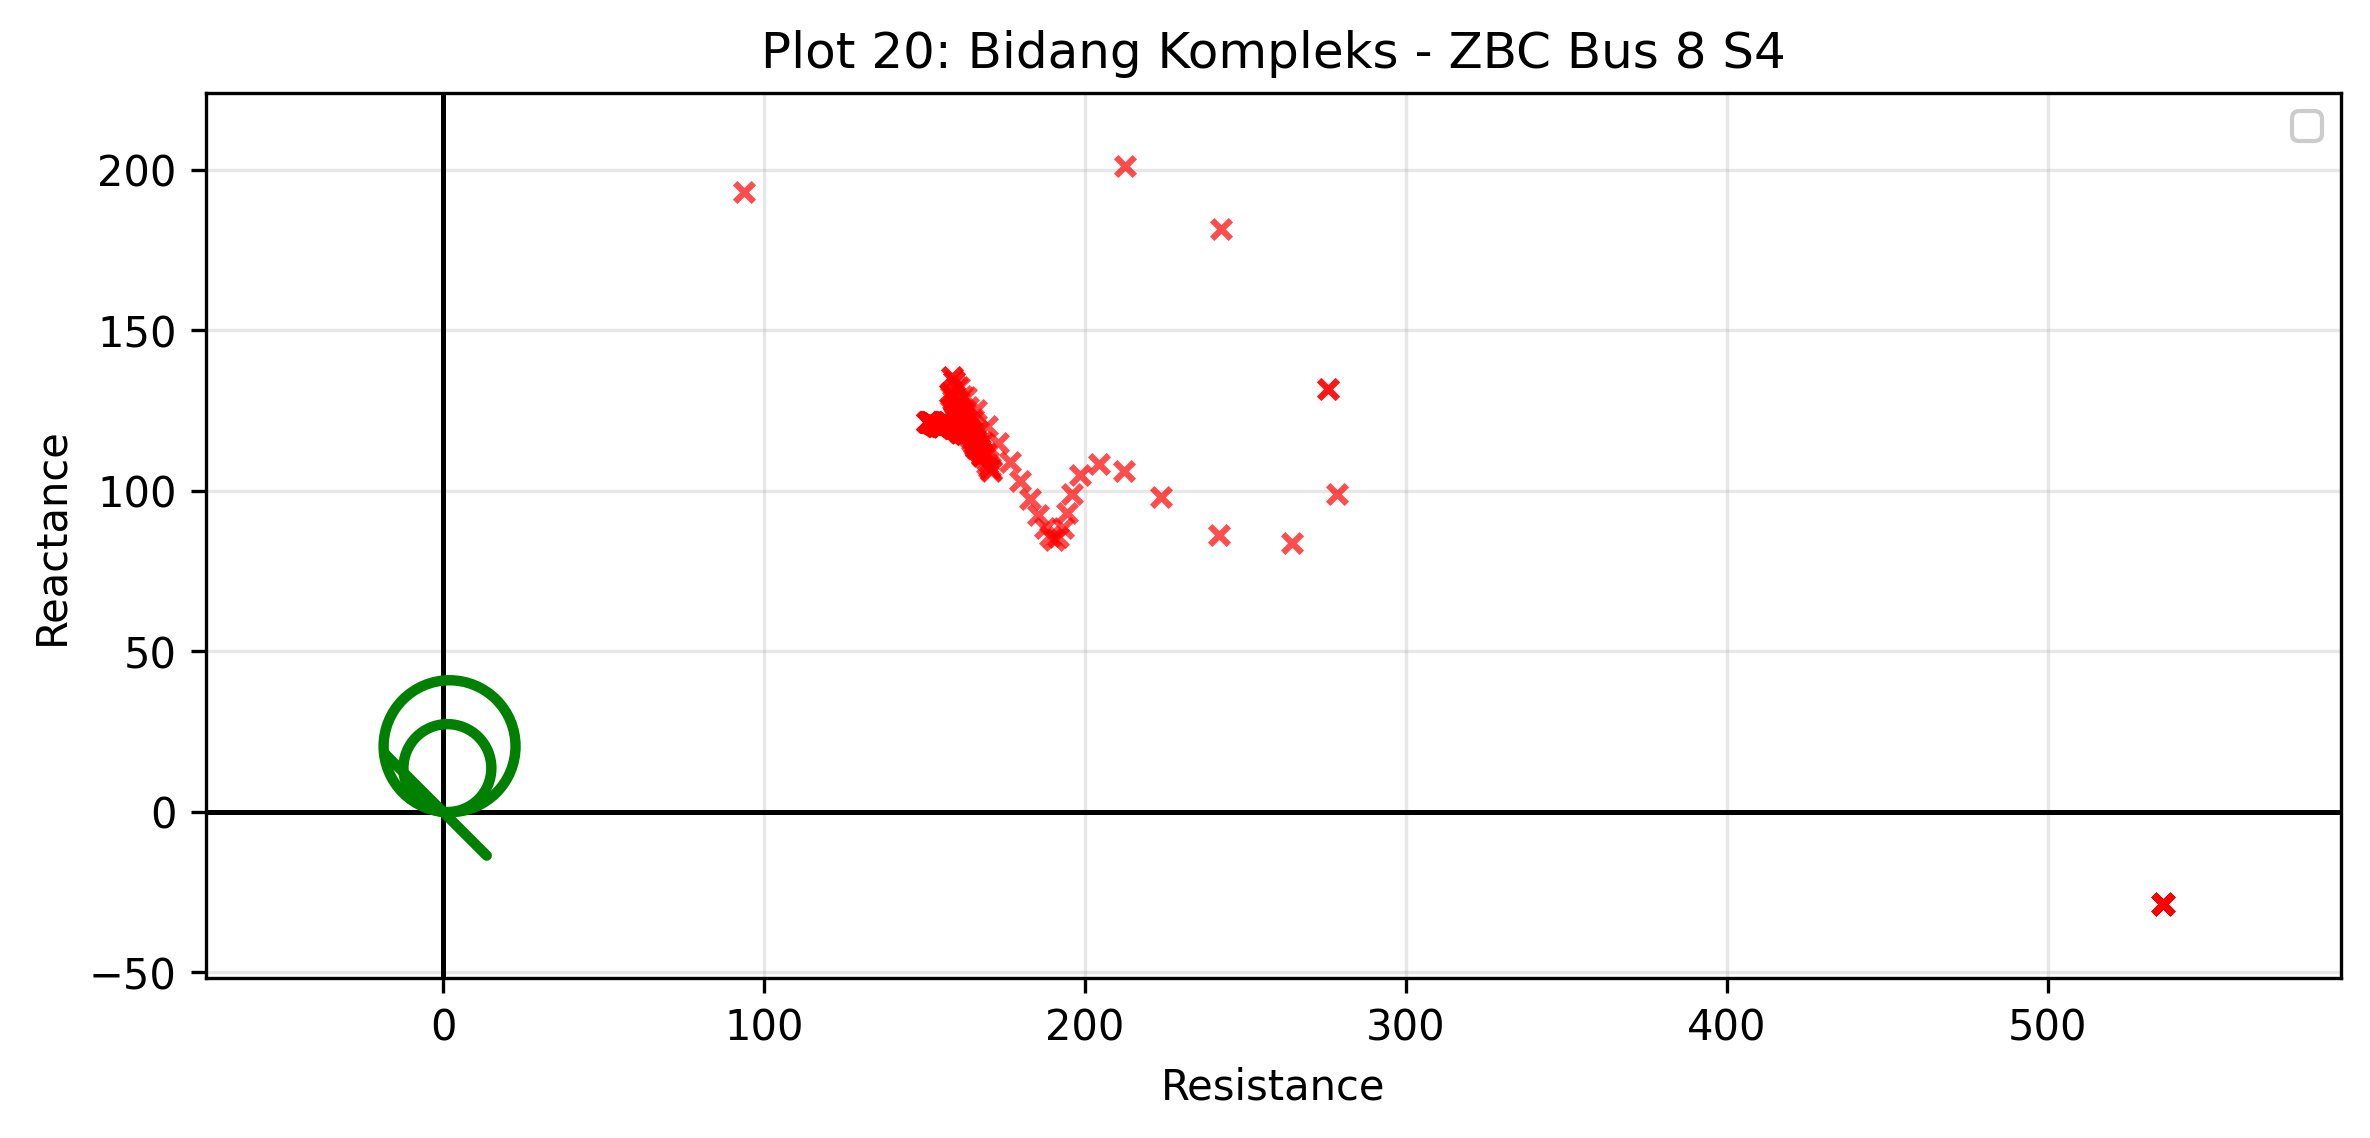
\includegraphics[width=0.8\textwidth]{contents/chapter-4/PRIA_20_ZBC_Bus_8_S4.png}
%     \caption{Impedansi Tampak ZBC Bus 8 Skenario 4}
%     \label{fig:PRIA_20_ZBC_Bus_8_S4}
% \end{figure}

% \begin{figure}[H]
%     \centering
%     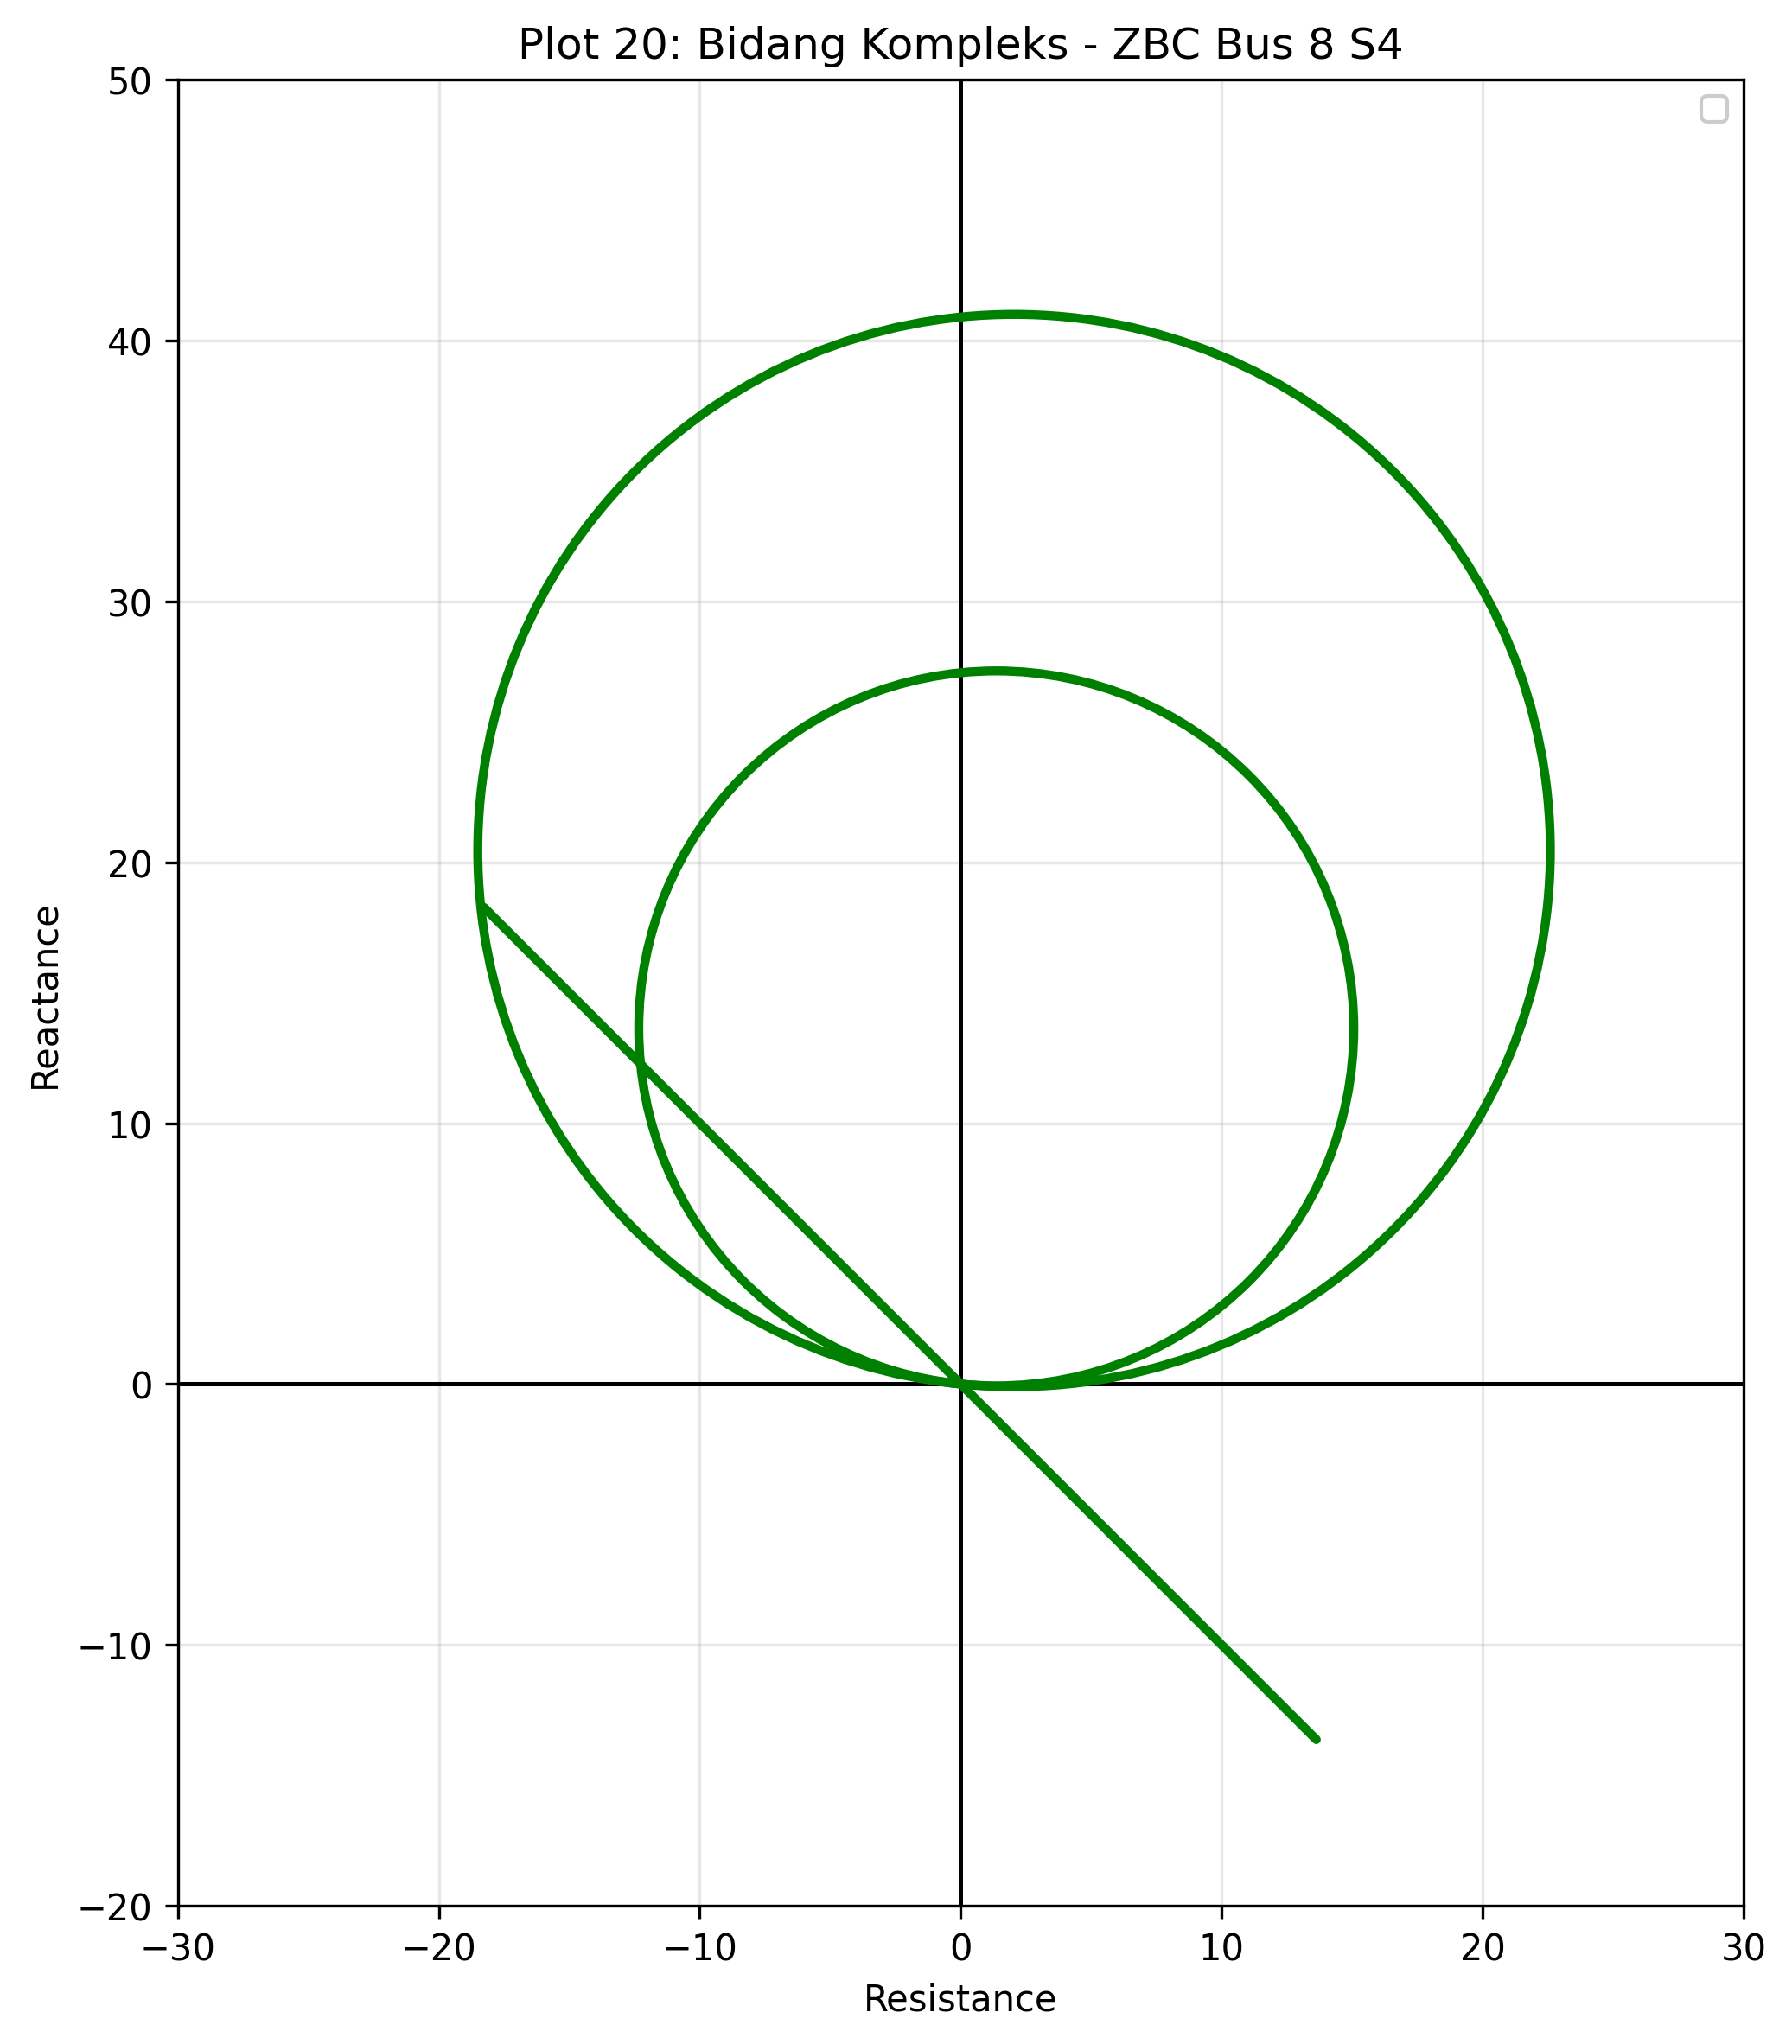
\includegraphics[width=0.8\textwidth]{contents/chapter-4/PRIZI_20_ZBC_Bus_8_S4.png}
%     \caption{Impedansi Tampak ZBC Bus 8 Skenario 4}
%     \label{fig:PRIZI_20_ZBC_Bus_8_S4}
% \end{figure}

\begin{figure}[H]
    \centering

    % Gambar sebelah kiri
    \begin{subfigure}[t]{0.48\textwidth}
        \centering
        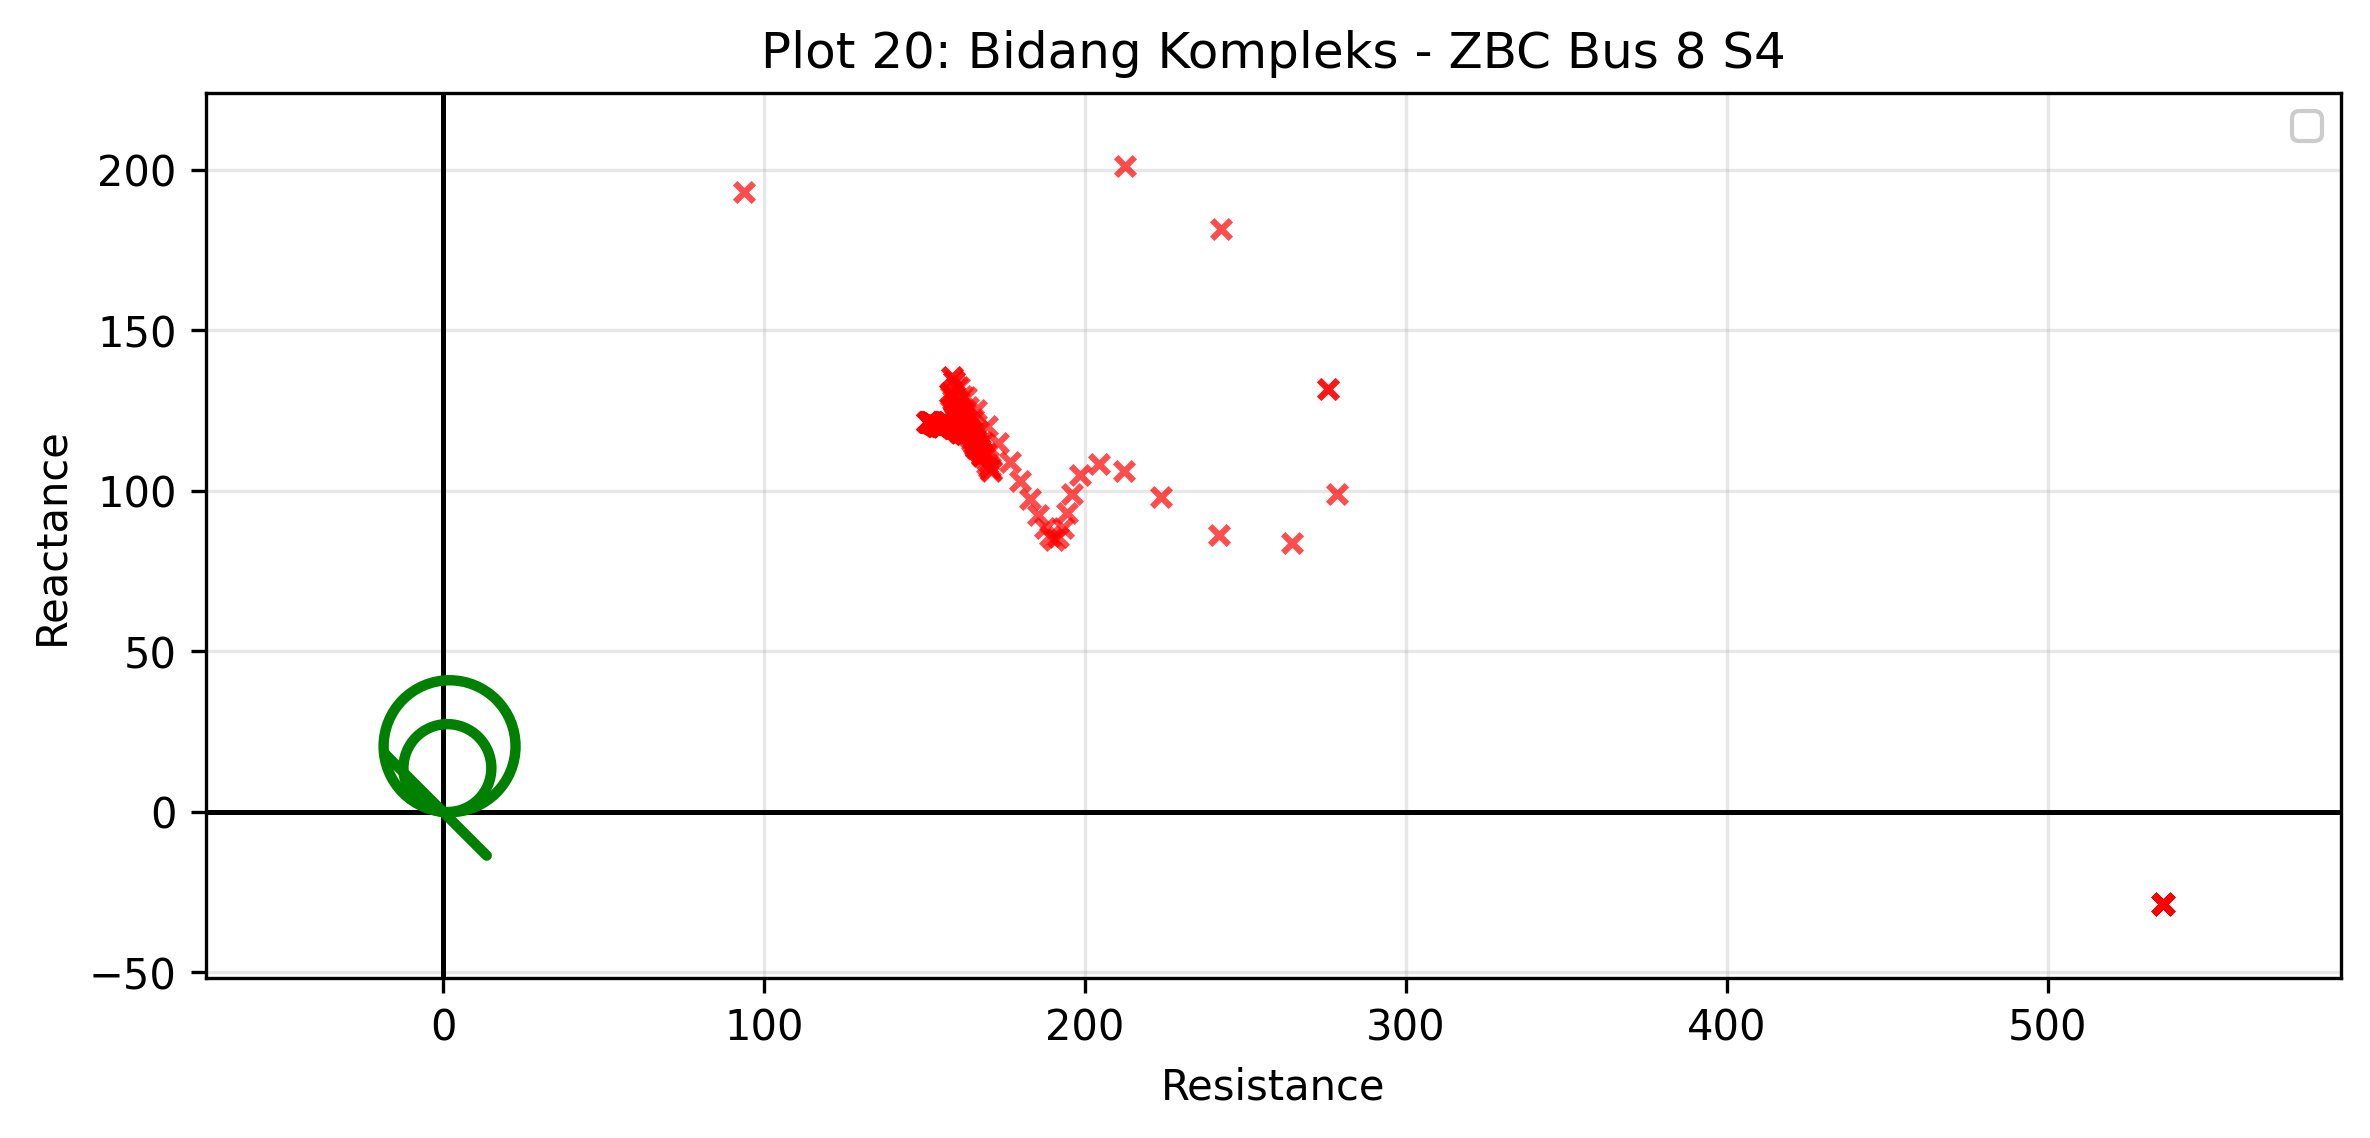
\includegraphics[width=\textwidth]{contents/chapter-4/PRIA_20_ZBC_Bus_8_S4.png}
        \caption{Seluruh Impedansi Tampak}
        \label{fig:PRIA_20_ZBC_Bus_8_S4}
    \end{subfigure}
    \hfill
    % Gambar sebelah kanan
    \begin{subfigure}[t]{0.48\textwidth}
        \centering
        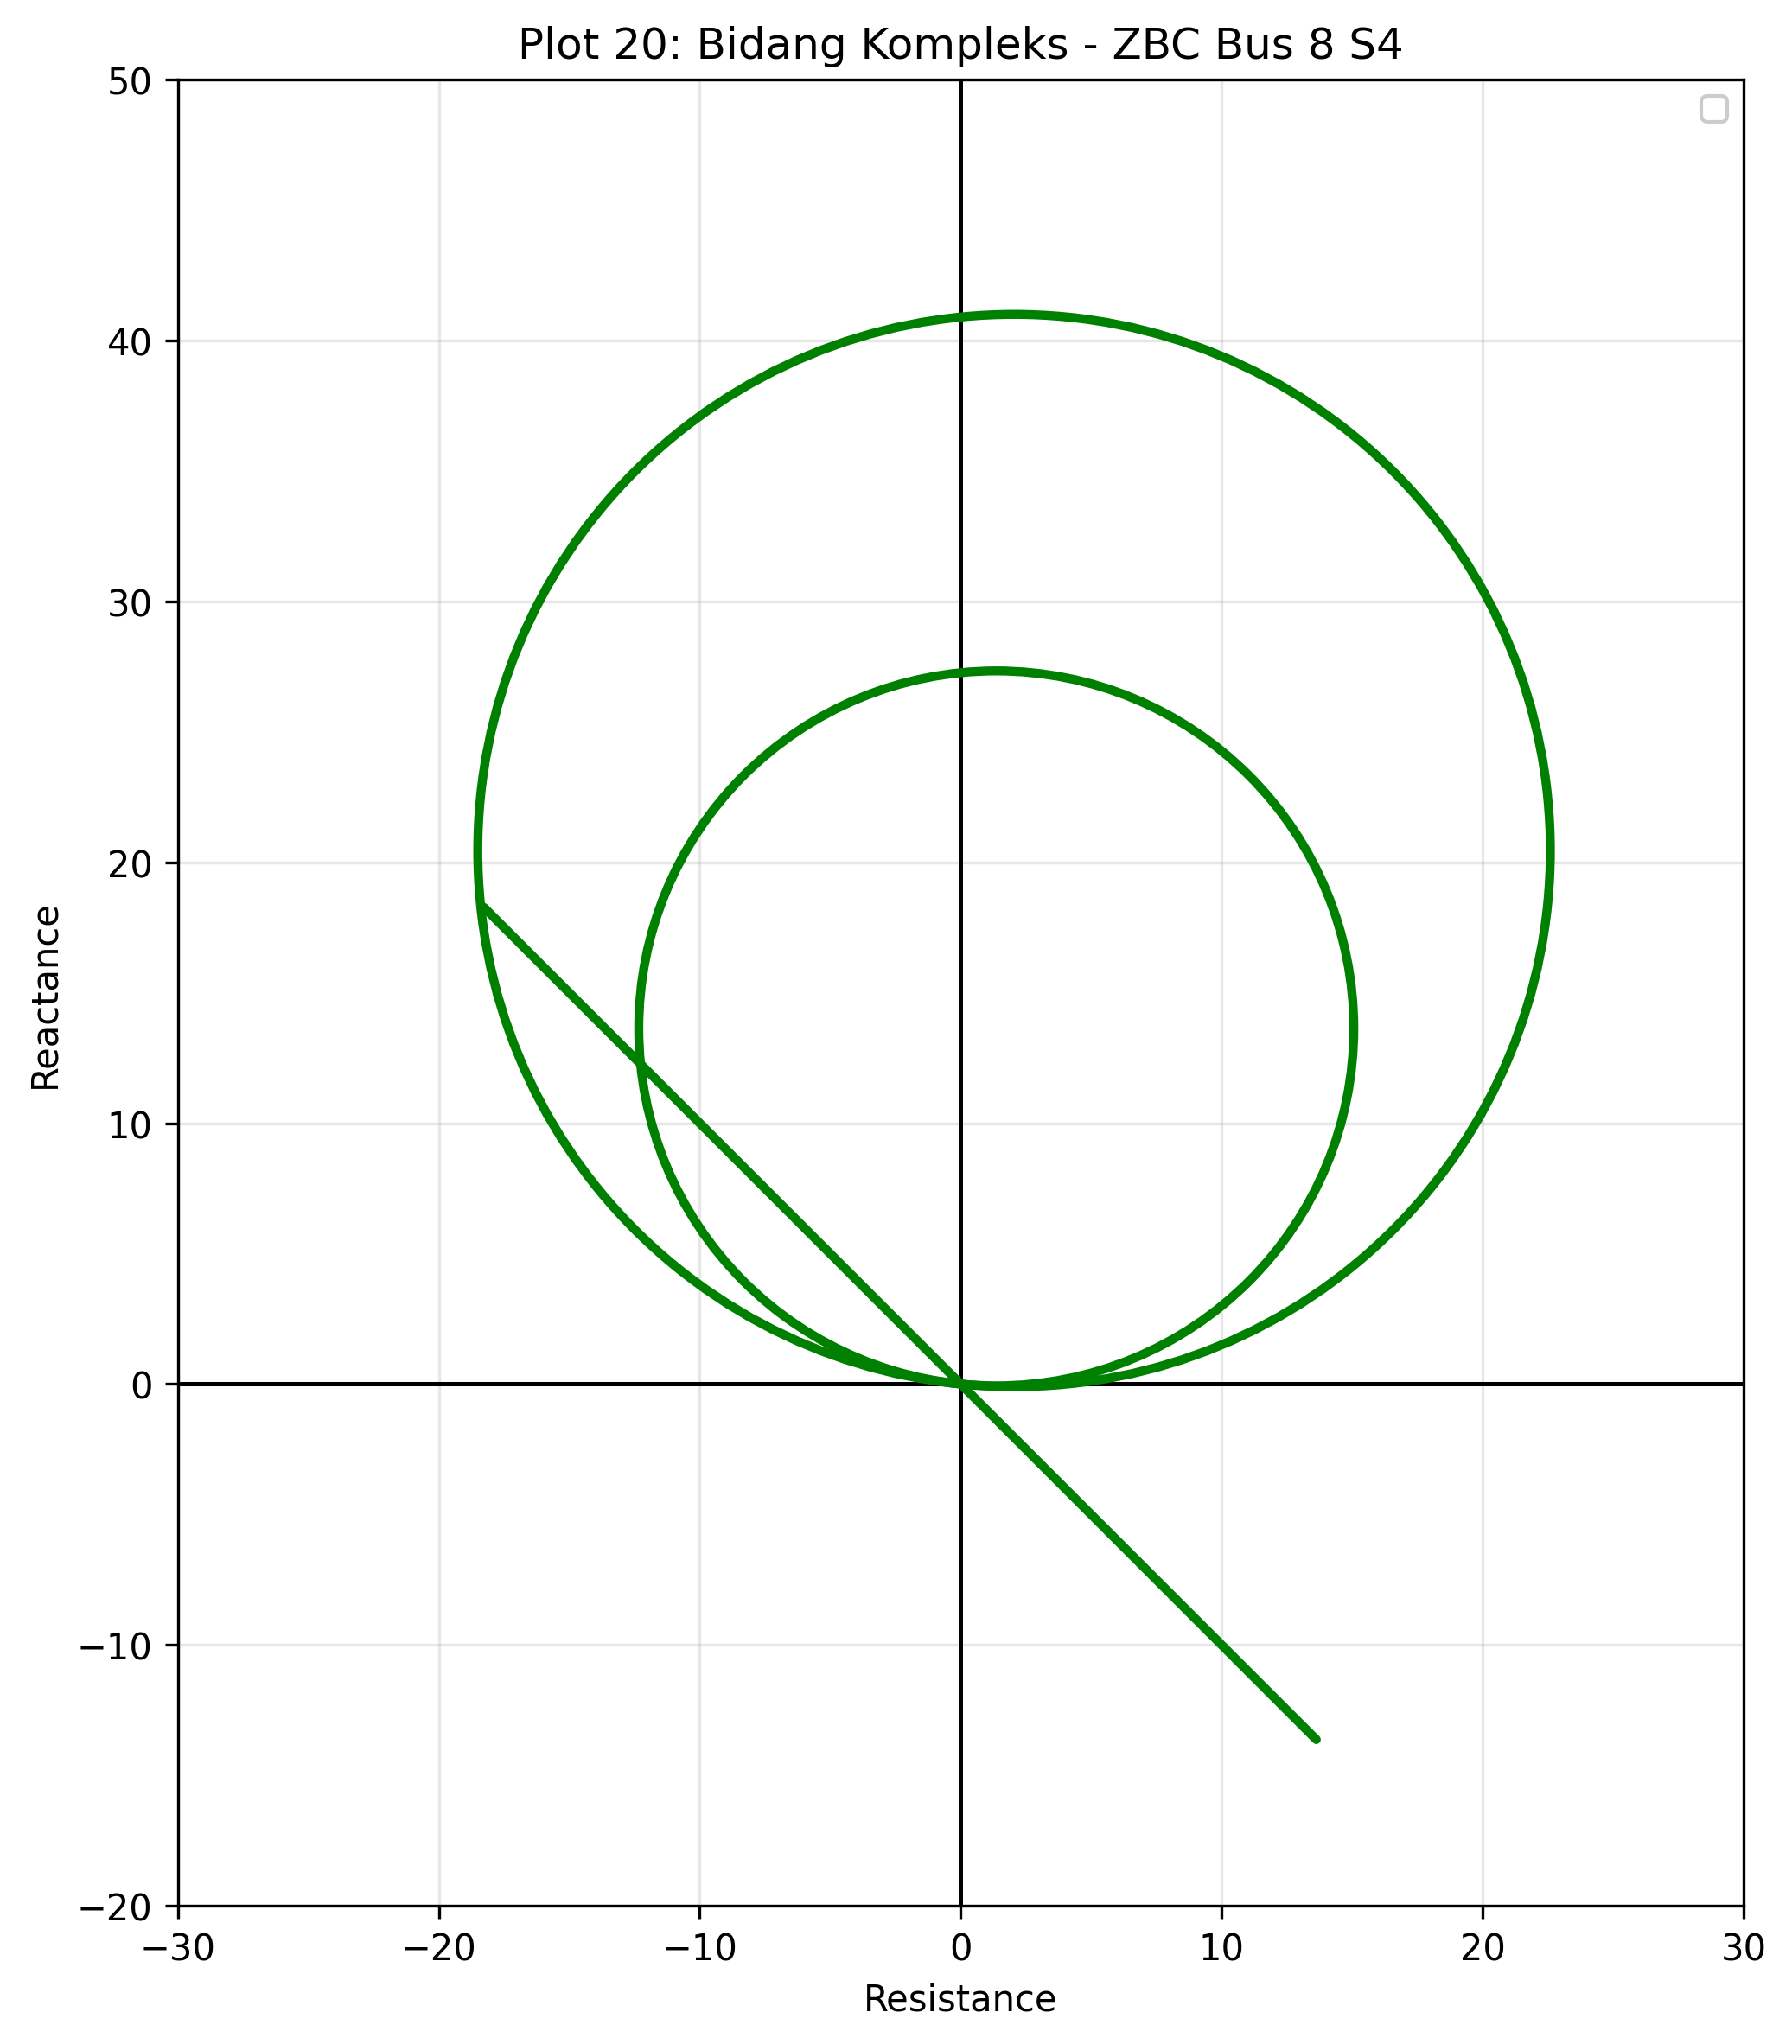
\includegraphics[width=\textwidth]{contents/chapter-4/PRIZI_20_ZBC_Bus_8_S4.png}
        \caption{Zoom In Pada Zona Proteksi}
        \label{fig:PRIZI_20_ZBC_Bus_8_S4}
    \end{subfigure}

    \caption{Impedansi Tampak ZBC Bus 8 Skenario 4}
    \label{fig:Impedansi_Tampak_ZBC_Bus_8_S4}
\end{figure}

Gambar \ref{fig:Impedansi_Tampak_ZBC_Bus_8_S4} menunjukkan bahwa impedansi tampak loop fasa B dengan fasa C yang dibaca oleh relay 21 sisi Bus 8 juga tidak masuk ke dalam zona proteksi. Hasil tersebut masih konsisten dengan arus sekunder CT pada Gambar \ref{fig:Bus_8_Ex_3P_S4}, yang menunjukkan bahwa arus gangguan belum memenuhi syarat \textit{starting} untuk membuat relay aktif. Oleh karena itu, jika dibandingkan dengan acuan gangguan eksternal tiga fasa pada Subbab \ref{subsec:tanpa_IBR_ex_3p}, respons relay 21 sisi Bus 8 pada elemen ini juga menunjukkan \textit{misoperation}.

%%%%%%%%%%%%%%%%%%%%%%%%%%%%%%%%%%%%%%%%%%%%%%%%%%%%%%%%%%%%%%%

% \begin{figure}[H]
%     \centering
%     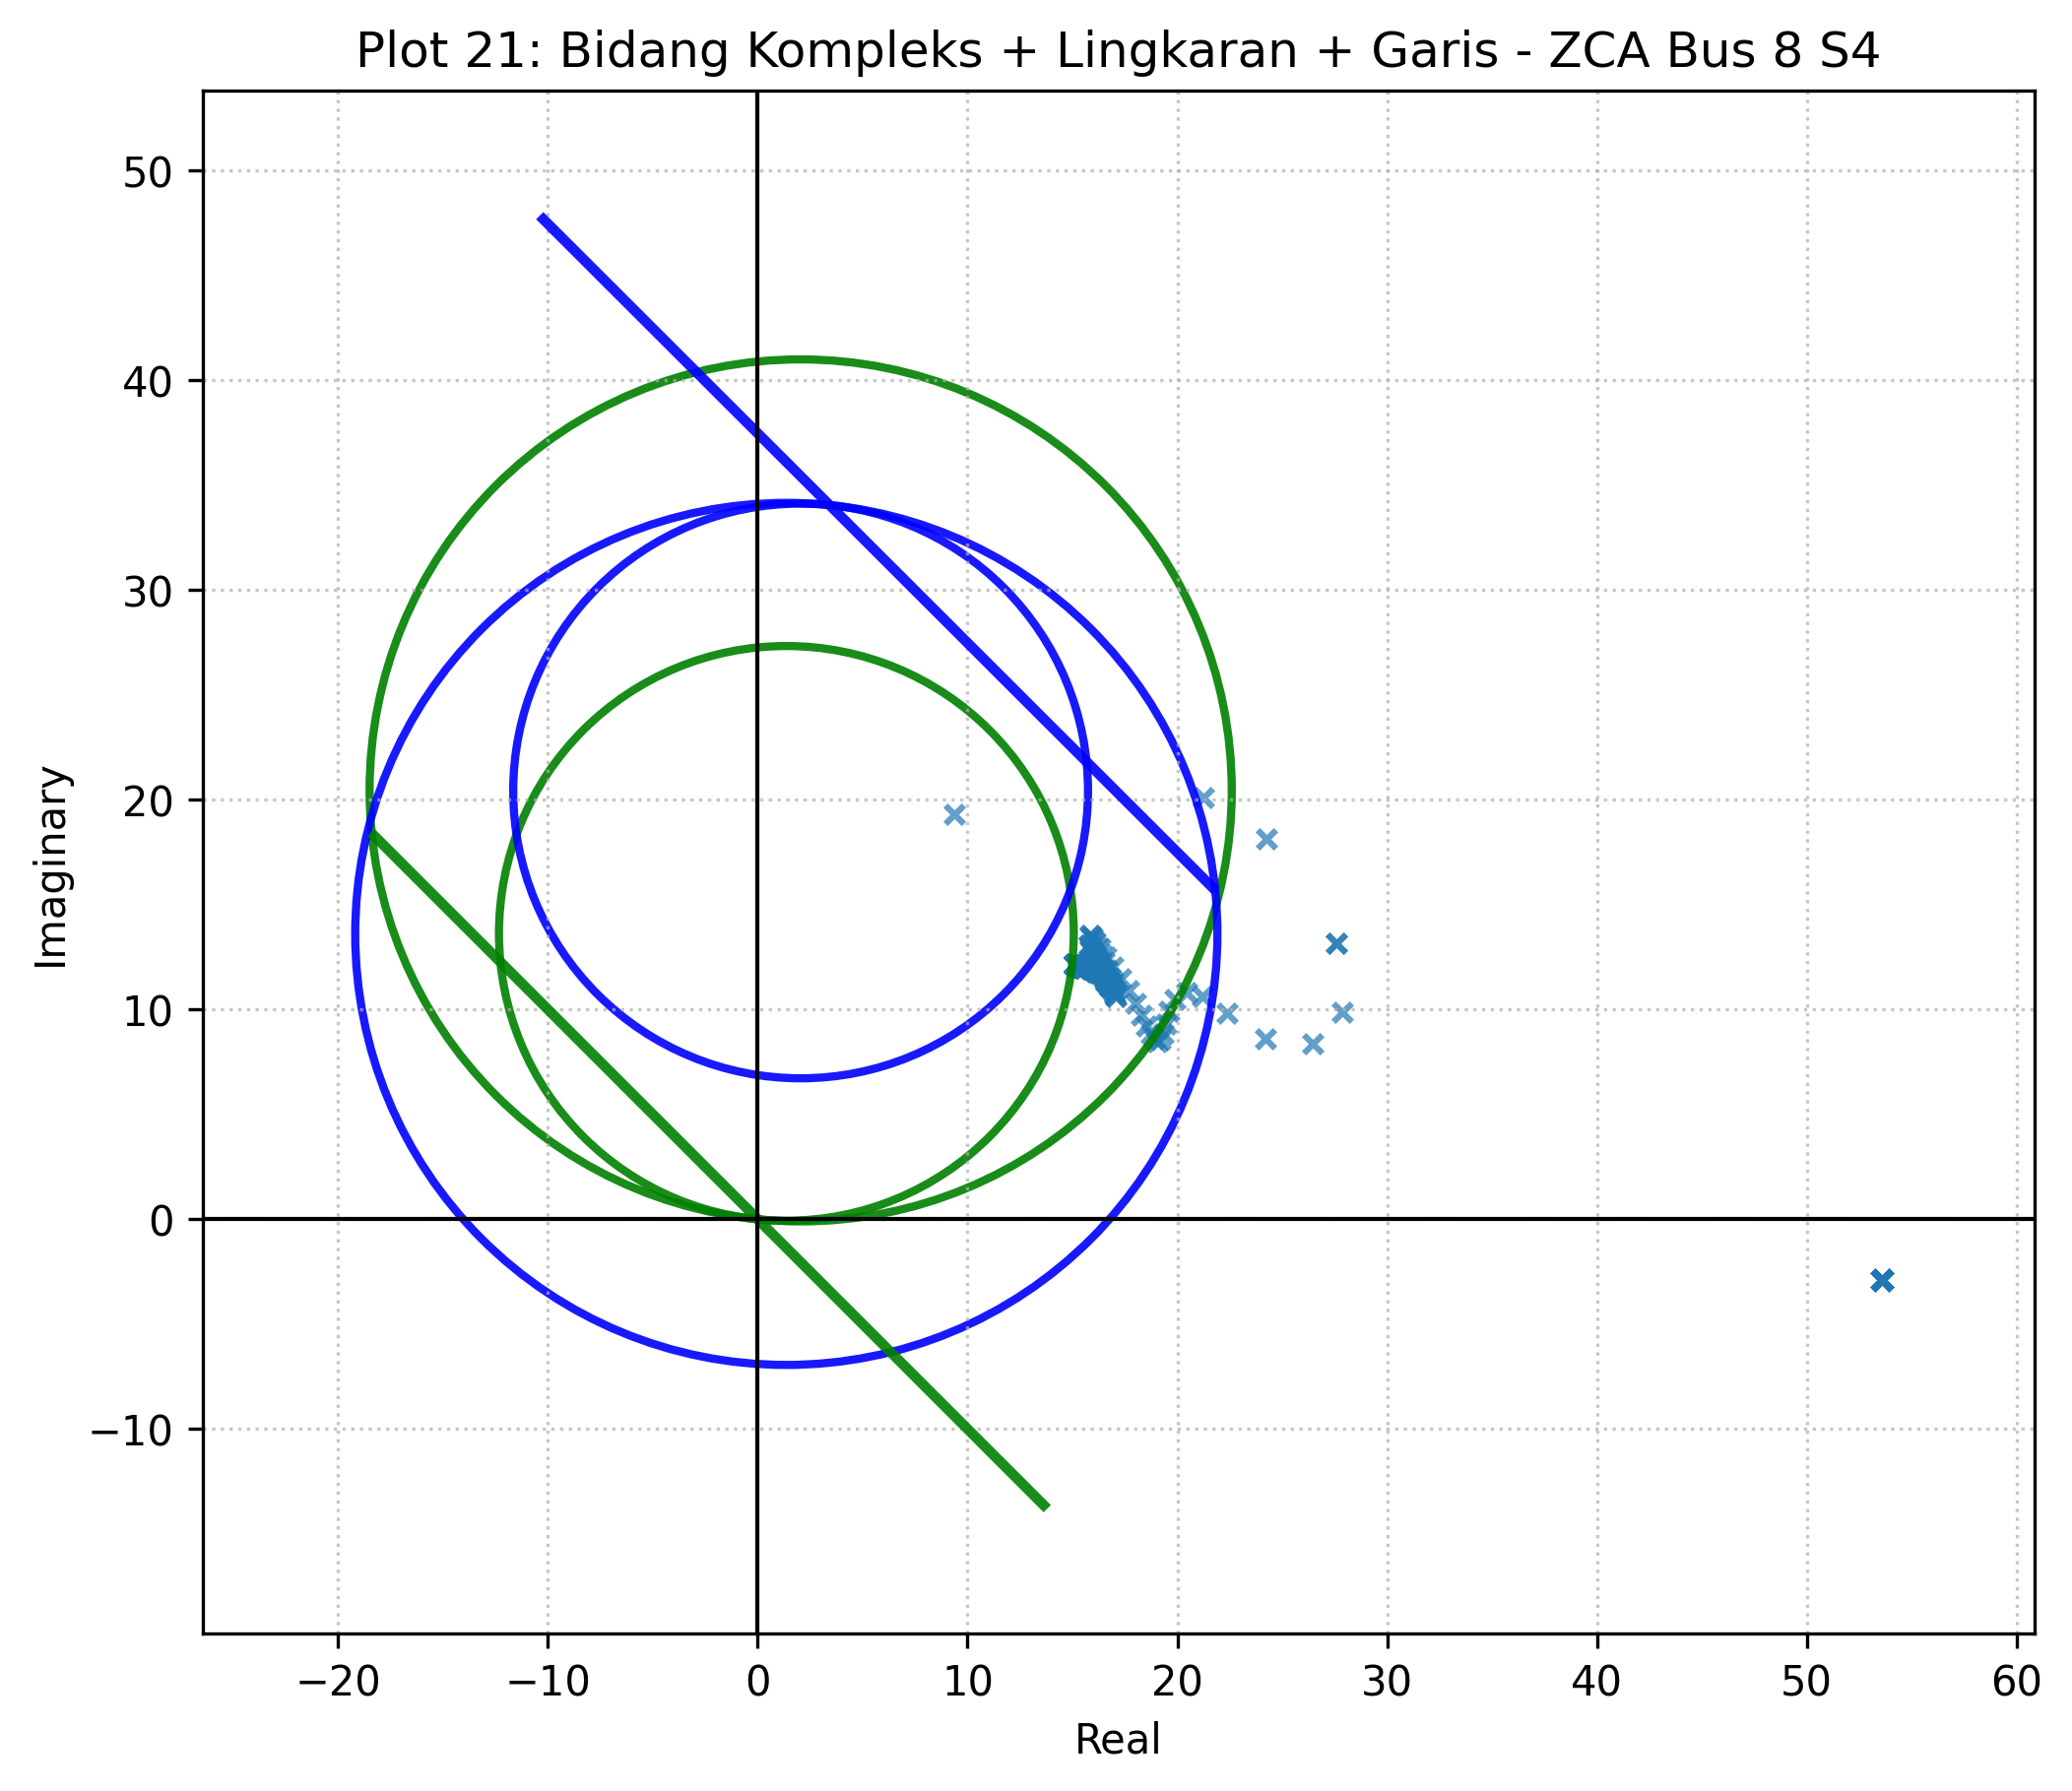
\includegraphics[width=0.8\textwidth]{contents/chapter-4/21_ZCA_Bus_8_S4_dengan_lingkaran_dan_garis.png}
%     \caption{Impedansi Tampak ZCA Bus 8 Skenario 4}
%     \label{fig:21_ZCA_Bus_8_S4_dengan_lingkaran_dan_garis}
% \end{figure}

% Terlihat pada gambar \ref{fig:21_ZCA_Bus_8_S4_dengan_lingkaran_dan_garis} bahwa impedansi tampak pada fasa C dengan fasa A yang dibaca oleh relay 21 sisi bus 8 saat terdapat gangguan mengalami over reach pada zona 1 serta mengalami drop out pada zona 2 sehingga dengan acuan pada \ref{subsec:tanpa_IBR_ex_3p} relay 21 bus 8 mengalami missoperation trip pada zona 1.

%%%%%%%%%%%%%%%%%%%%%%%%%%%%%%%%%SISI PRIMER%%%%%%%%%%%%%%%%%%%%%%%%%%%%%%%%%%

% \begin{figure}[H]
%     \centering
%     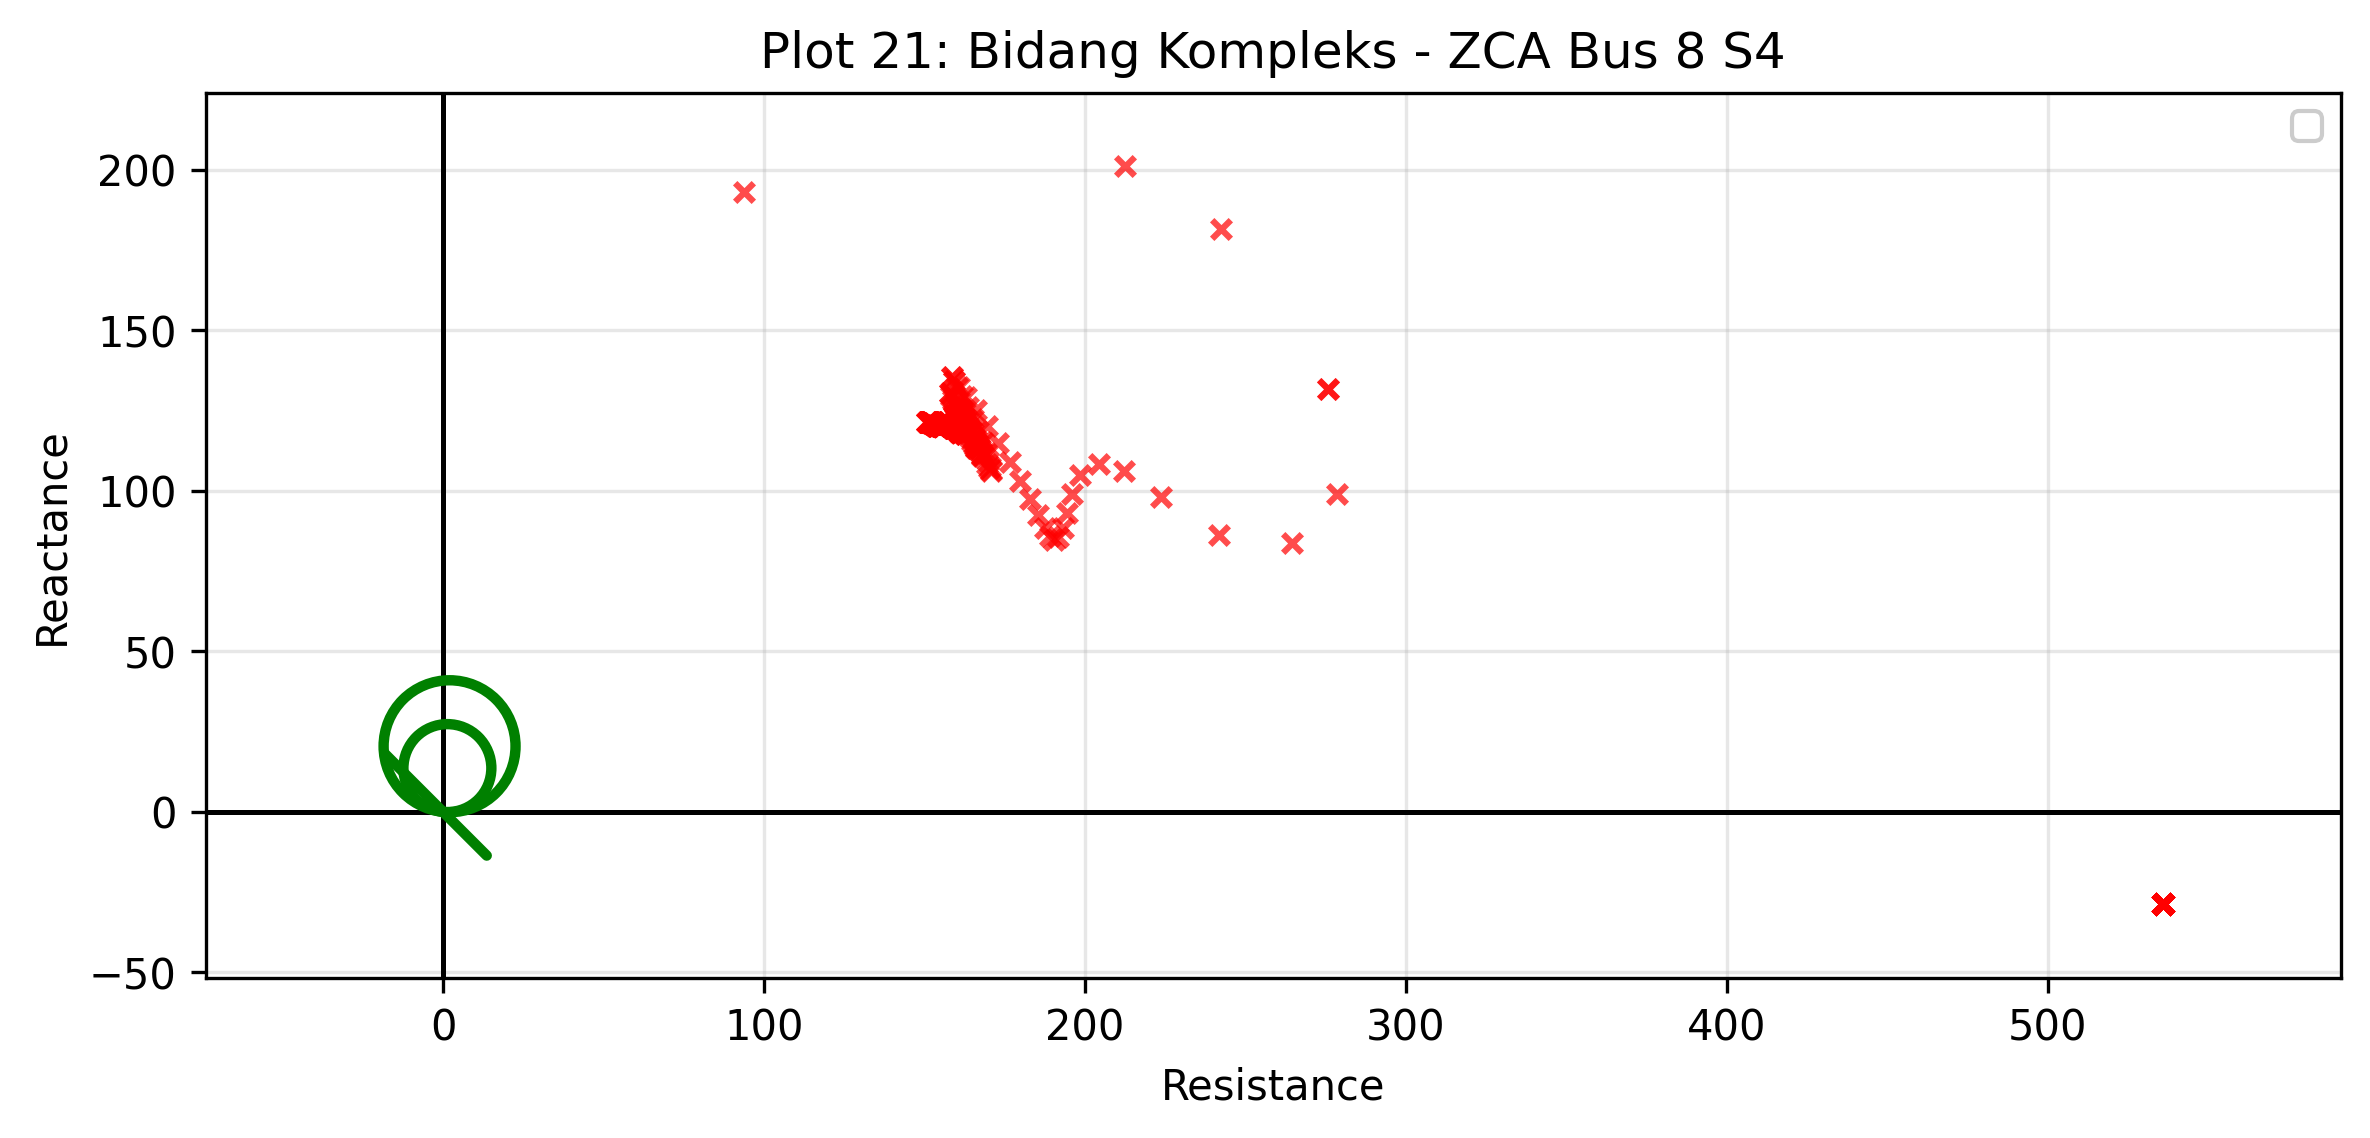
\includegraphics[width=0.8\textwidth]{contents/chapter-4/PRIA_21_ZCA_Bus_8_S4.png}
%     \caption{Impedansi Tampak ZCA Bus 8 Skenario 4}
%     \label{fig:PRIA_21_ZCA_Bus_8_S4}
% \end{figure}

% \begin{figure}[H]
%     \centering
%     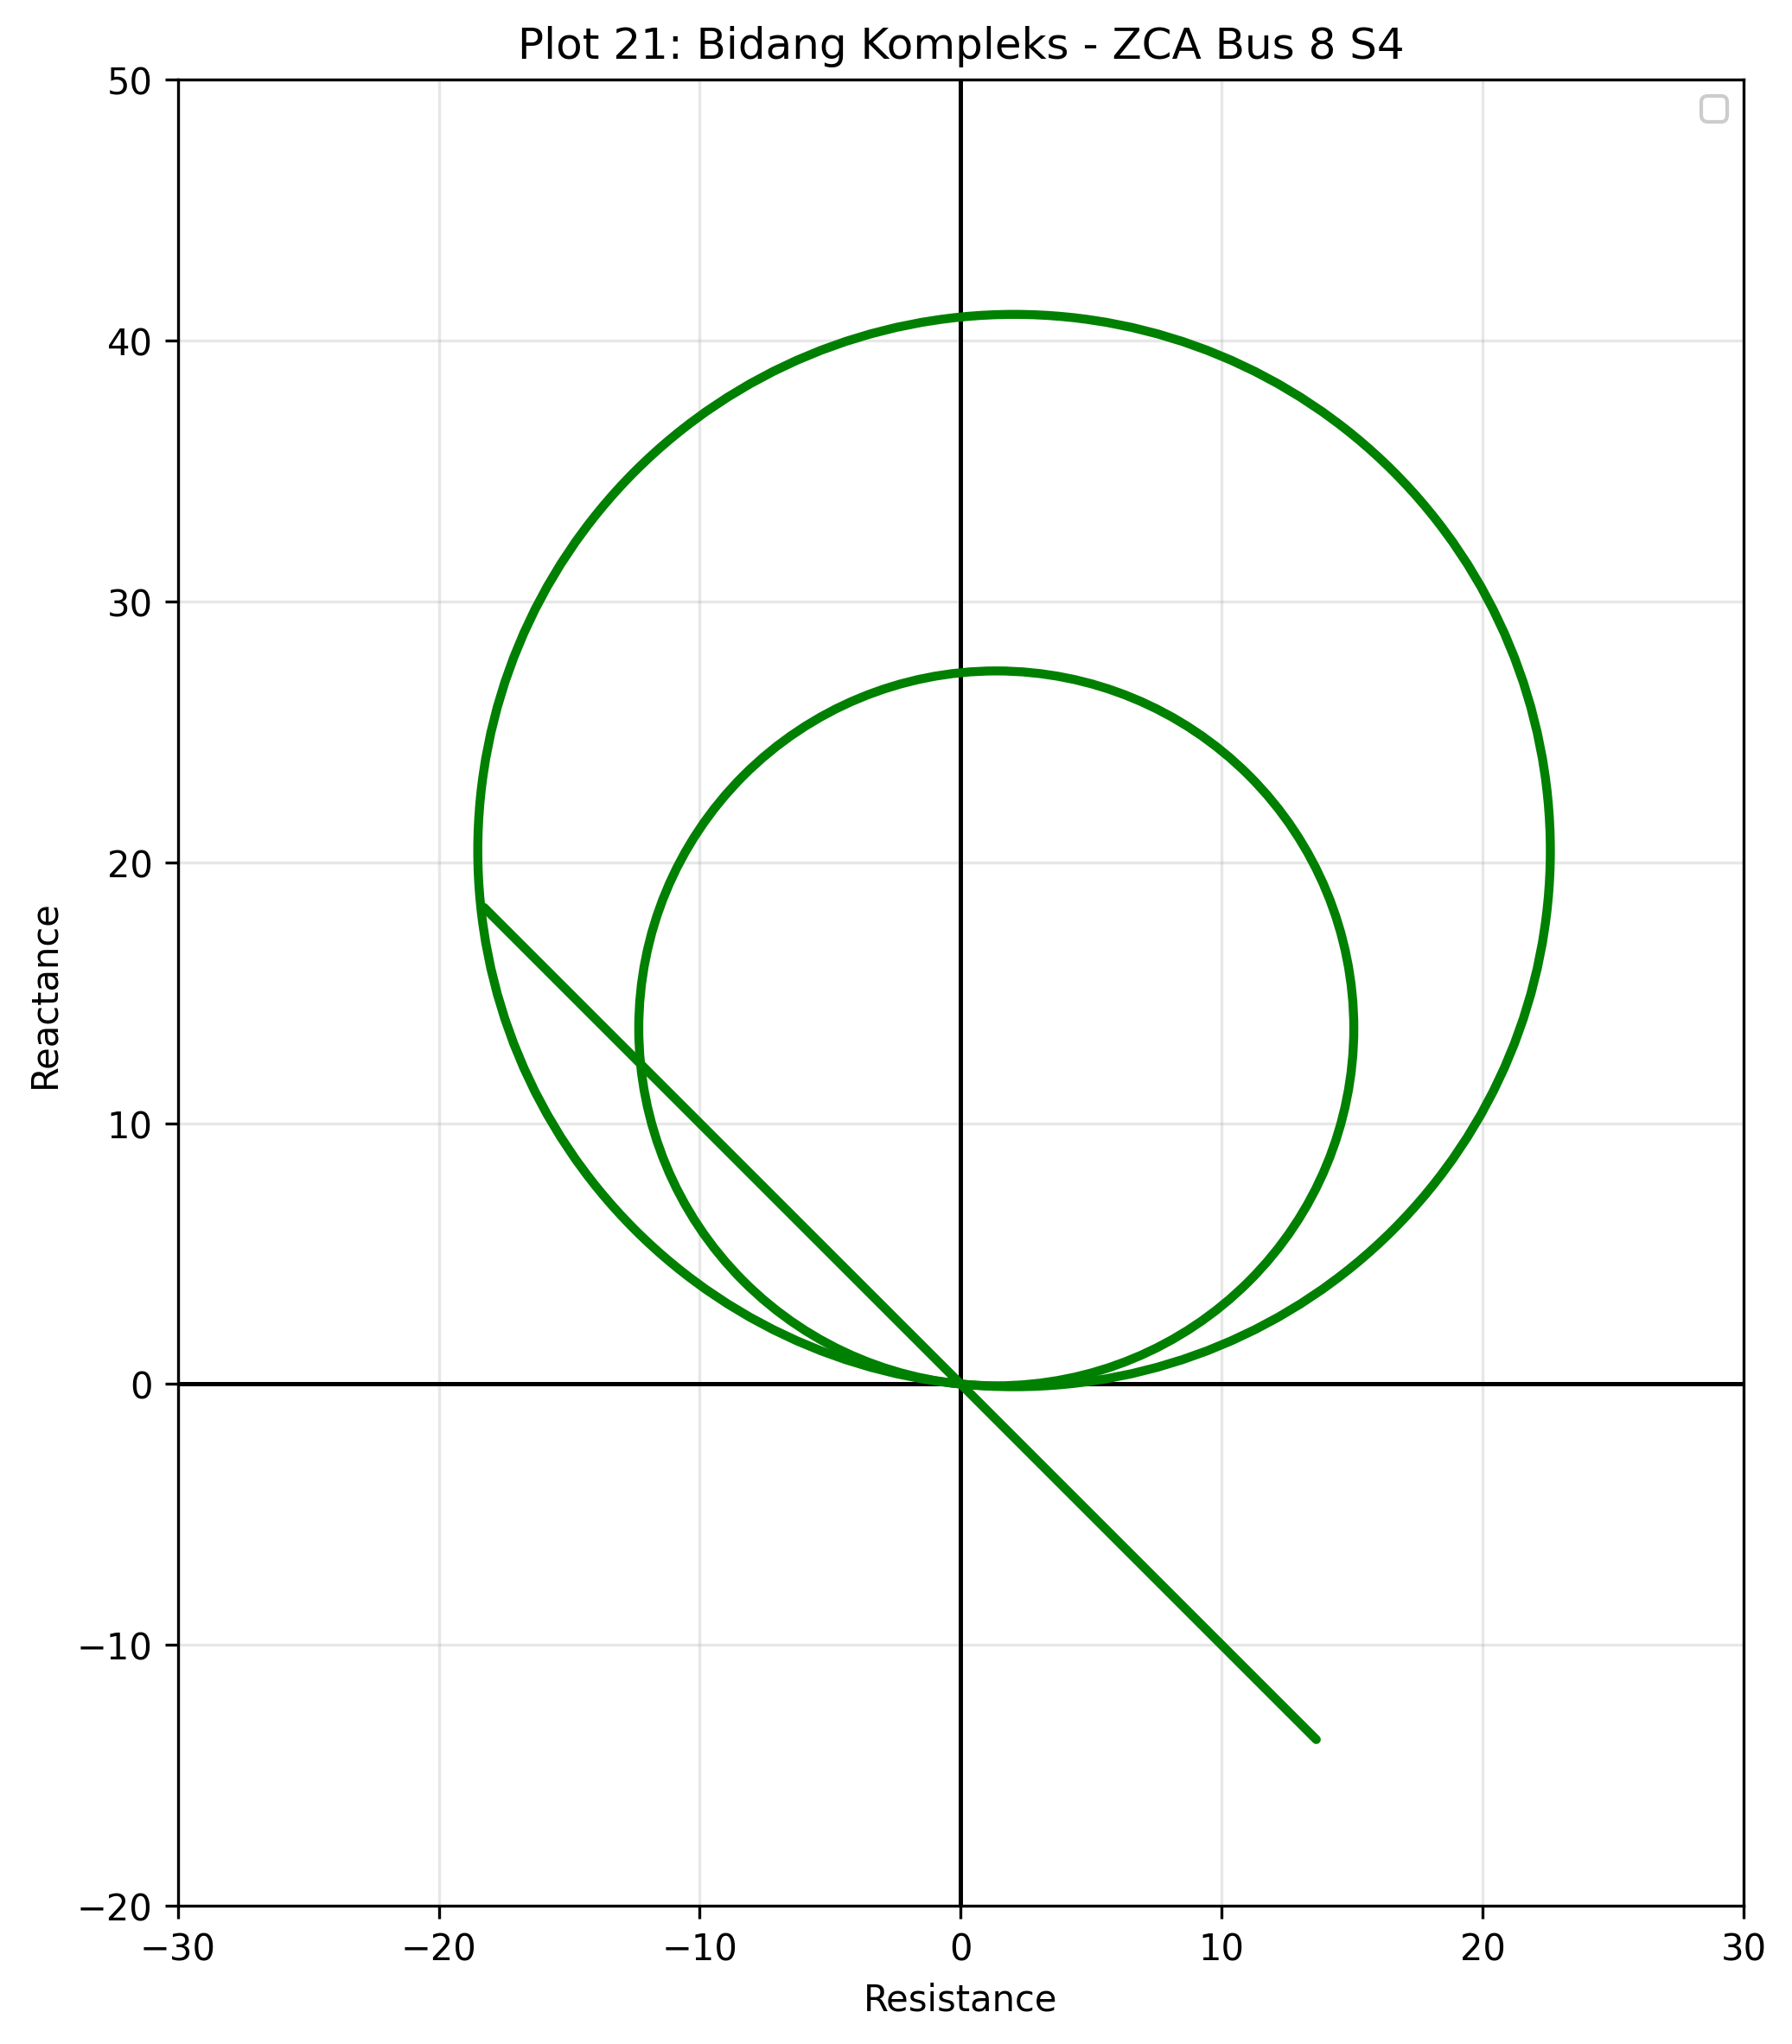
\includegraphics[width=0.8\textwidth]{contents/chapter-4/PRIZI_21_ZCA_Bus_8_S4.png}
%     \caption{Impedansi Tampak ZCA Bus 8 Skenario 4}
%     \label{fig:PRIZI_21_ZCA_Bus_8_S4}
% \end{figure}

\begin{figure}[H]
    \centering

    % Gambar sebelah kiri
    \begin{subfigure}[t]{0.48\textwidth}
        \centering
        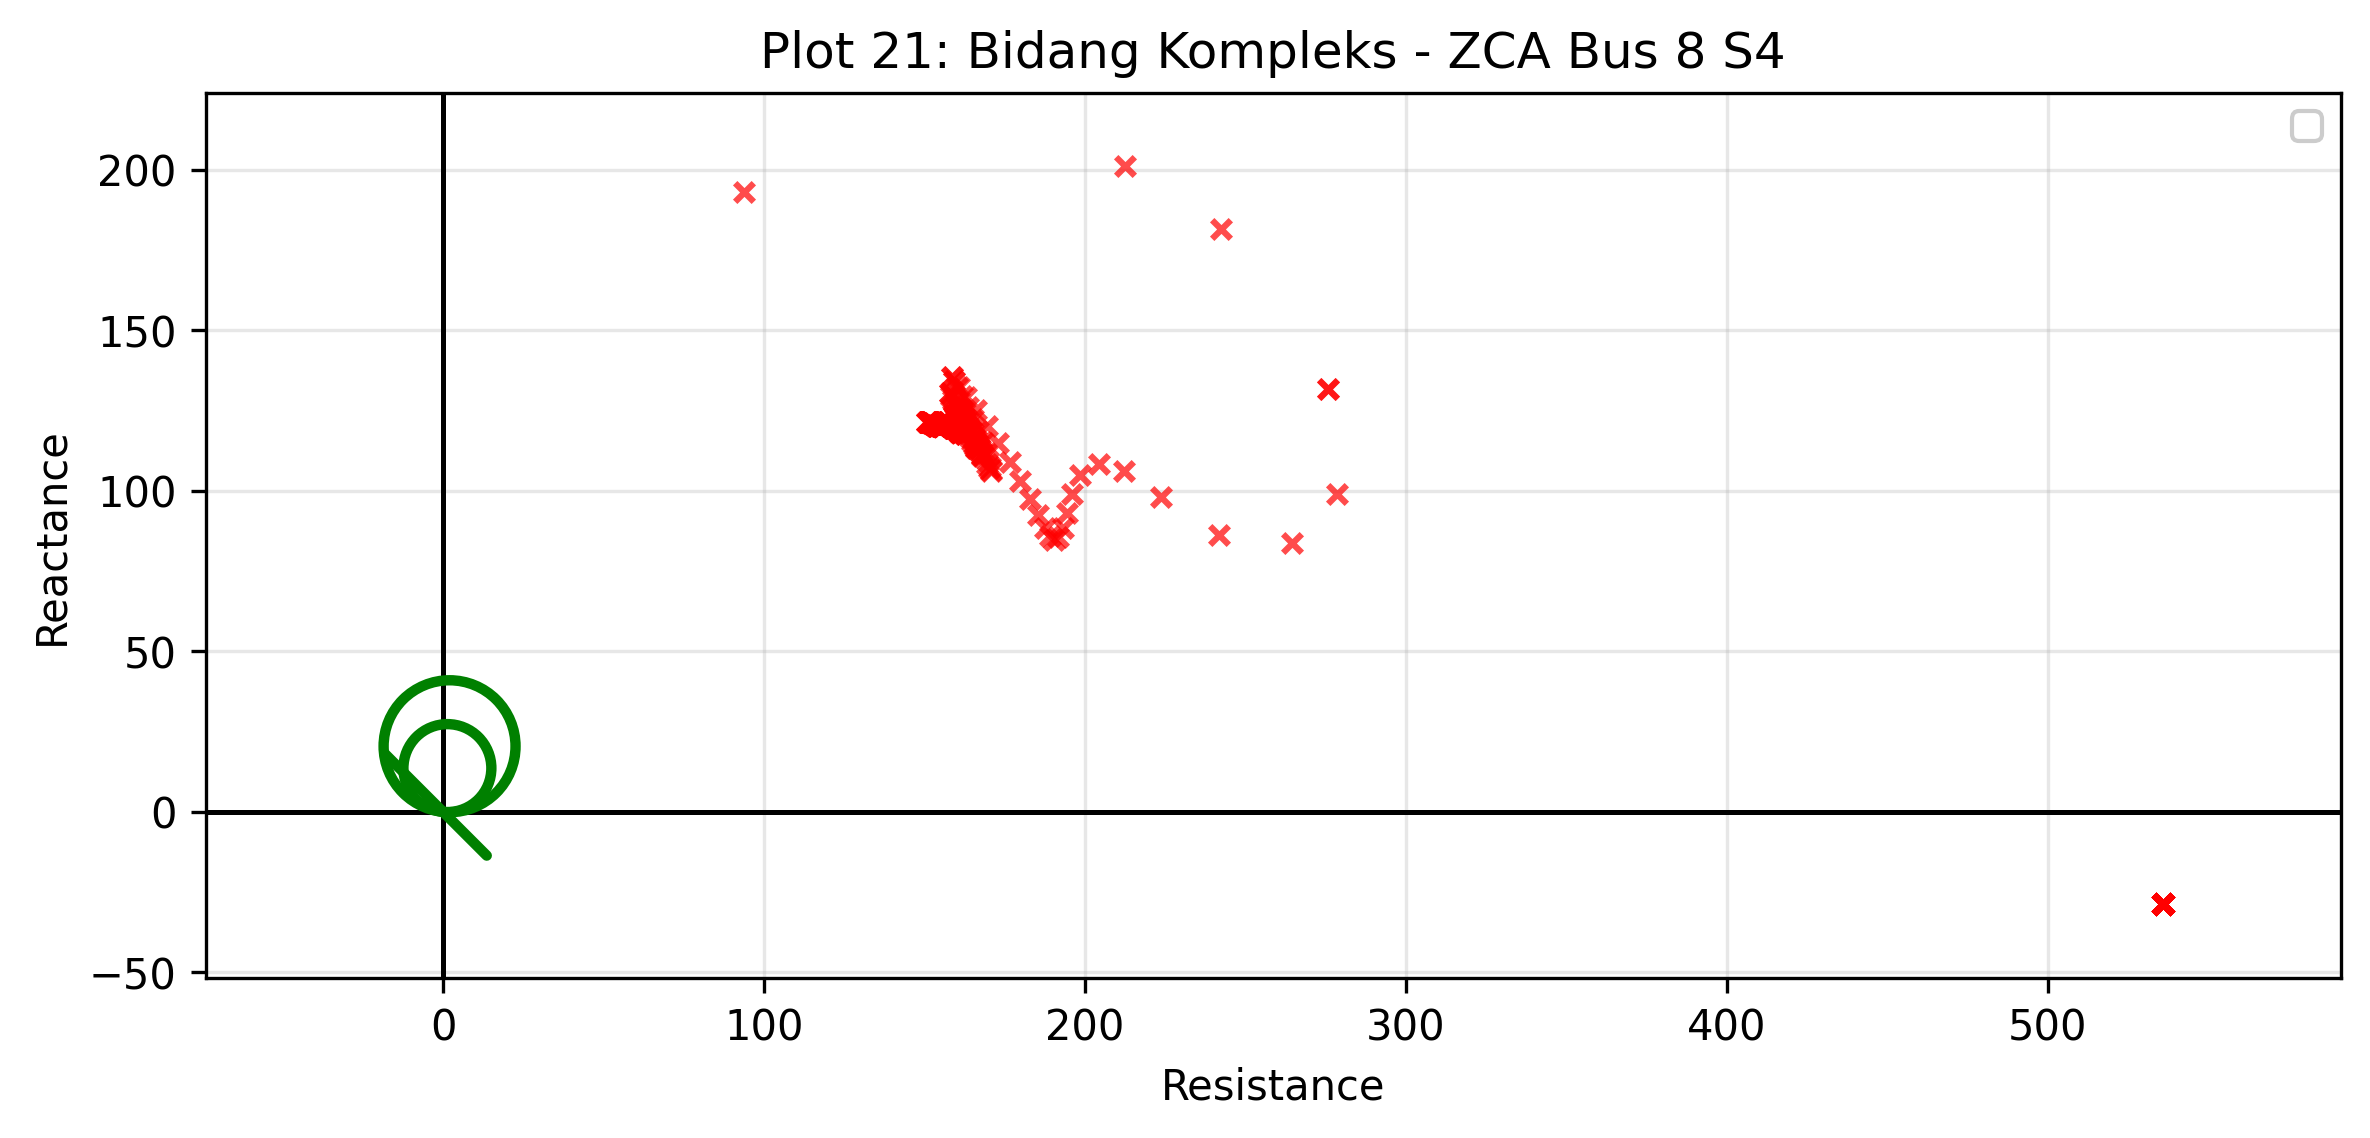
\includegraphics[width=\textwidth]{contents/chapter-4/PRIA_21_ZCA_Bus_8_S4.png}
        \caption{Seluruh Impedansi Tampak}
        \label{fig:PRIA_21_ZCA_Bus_8_S4}
    \end{subfigure}
    \hfill
    % Gambar sebelah kanan
    \begin{subfigure}[t]{0.48\textwidth}
        \centering
        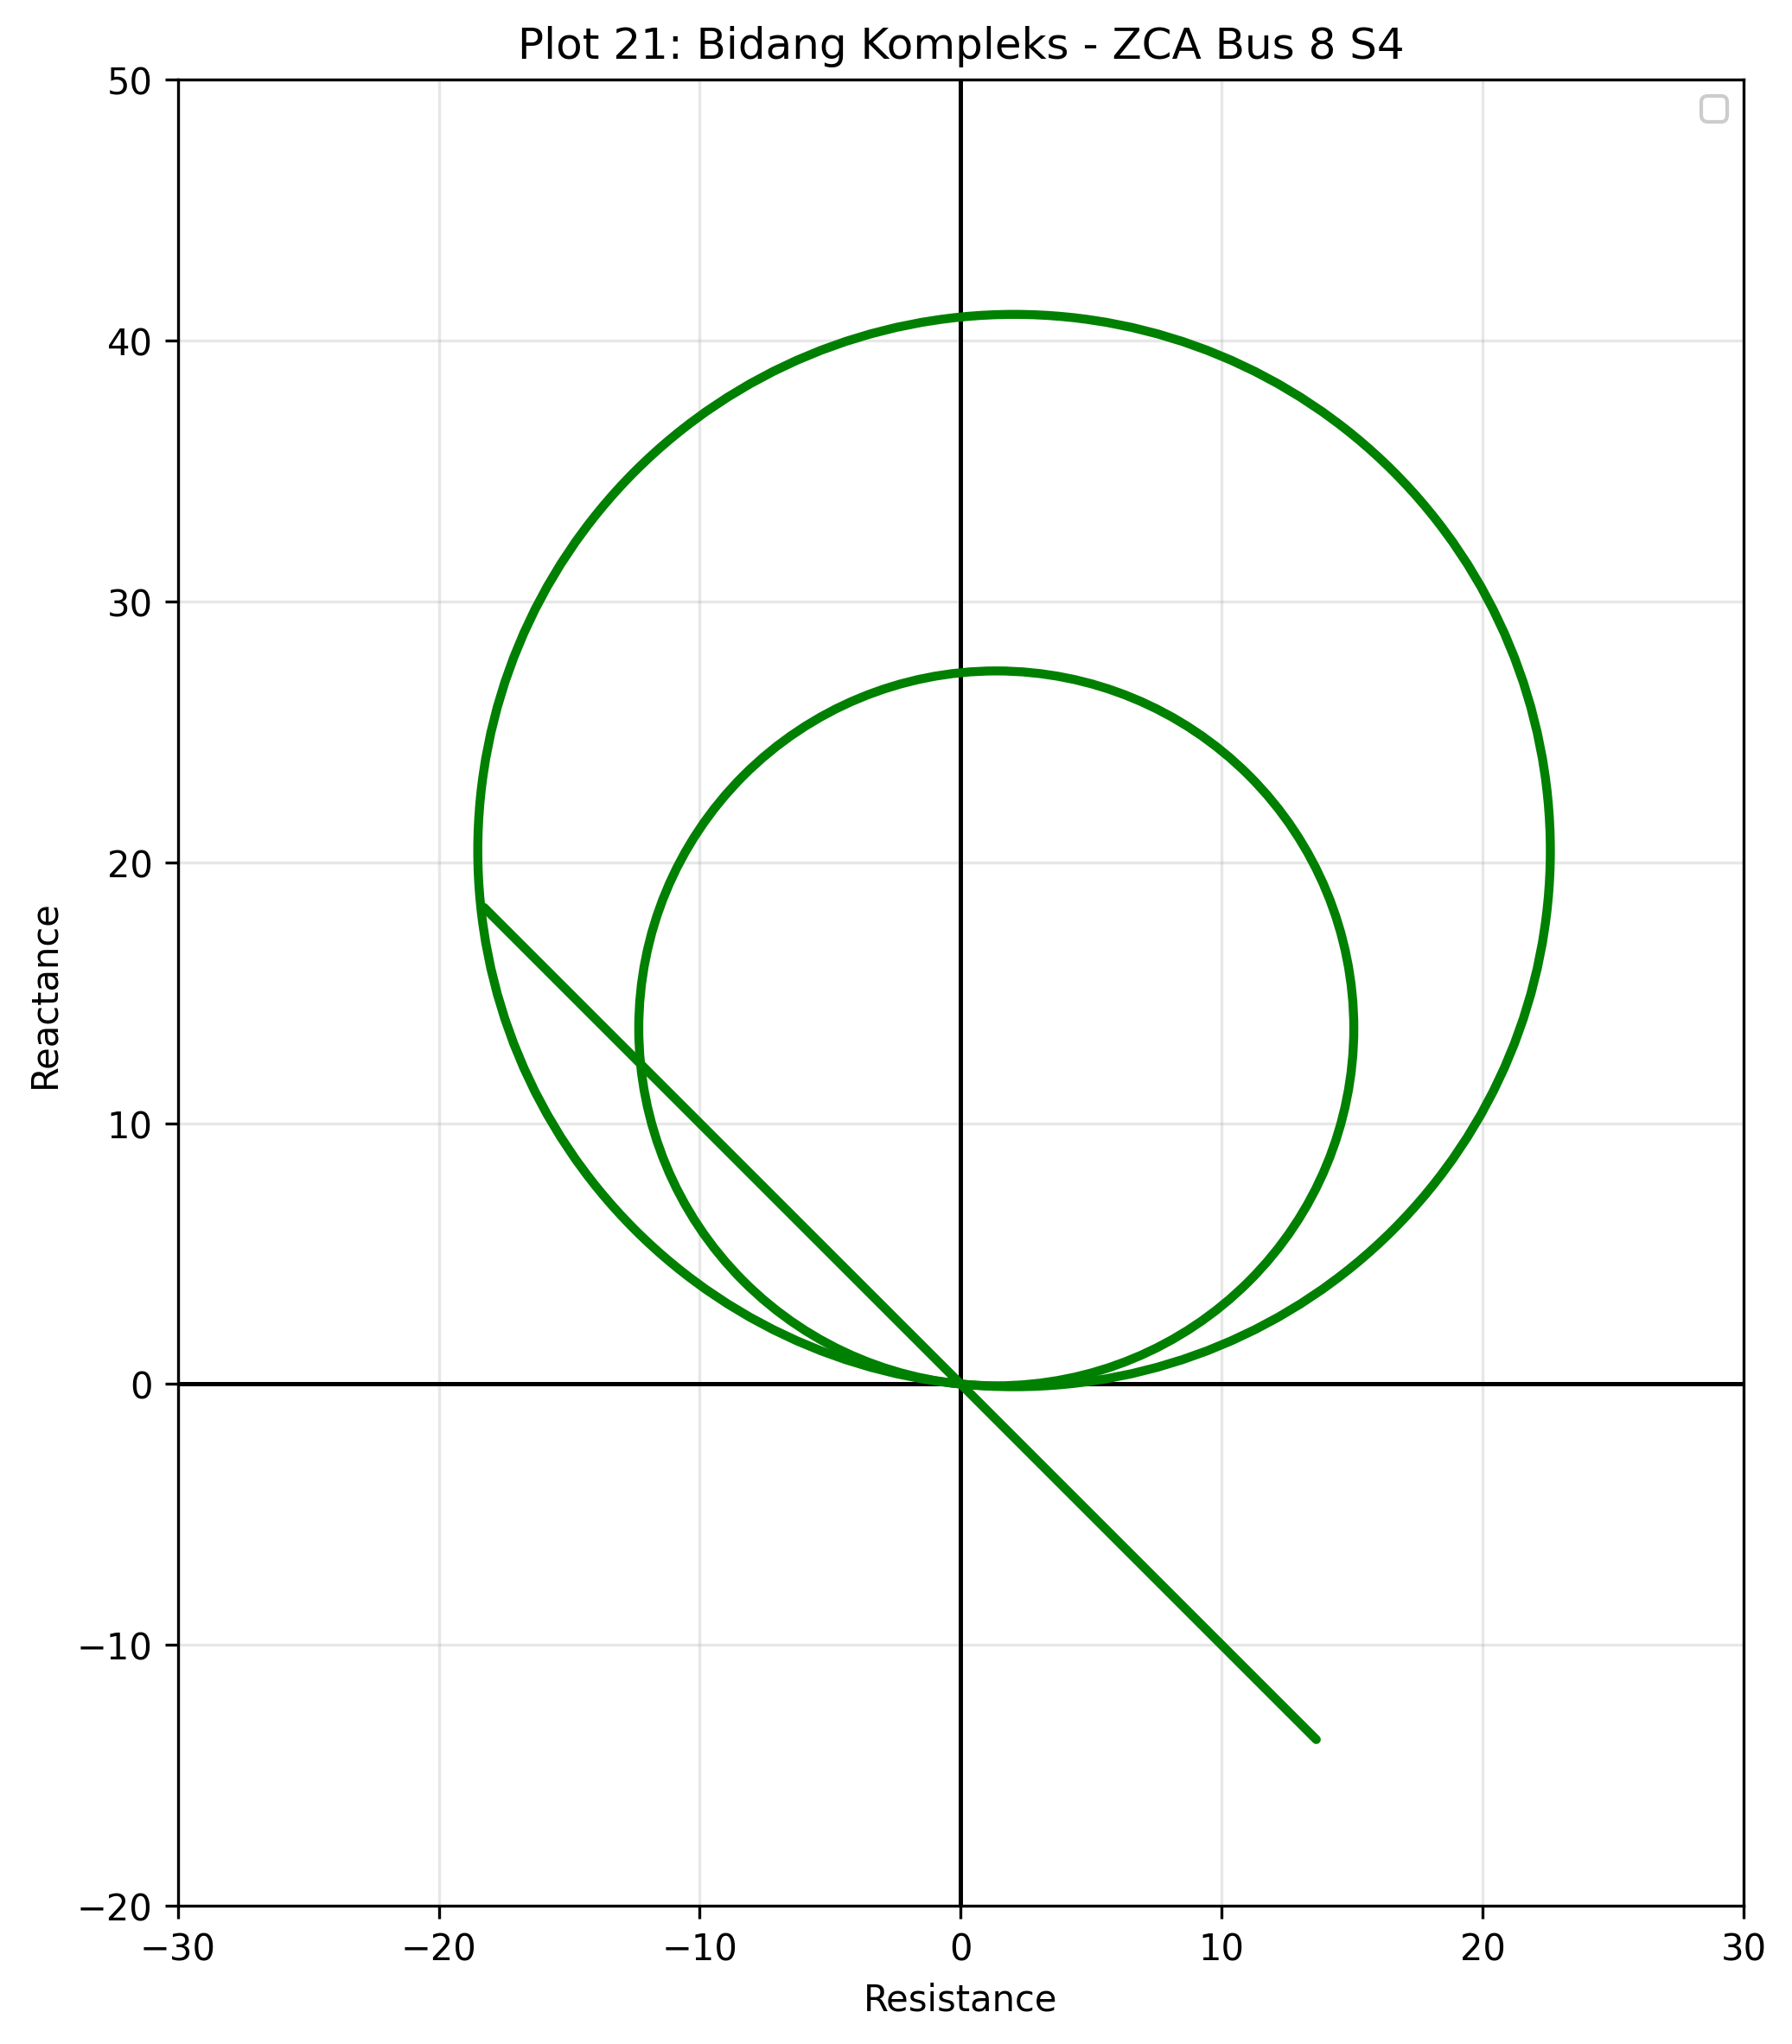
\includegraphics[width=\textwidth]{contents/chapter-4/PRIZI_21_ZCA_Bus_8_S4.png}
        \caption{Zoom In Pada Zona Proteksi}
        \label{fig:PRIZI_21_ZCA_Bus_8_S4}
    \end{subfigure}

    \caption{Impedansi Tampak ZCA Bus 8 Skenario 4}
    \label{fig:Impedansi_Tampak_ZCA_Bus_8_S4}
\end{figure}

Gambar \ref{fig:Impedansi_Tampak_ZCA_Bus_8_S4} menunjukkan bahwa impedansi tampak loop fasa C dengan fasa A yang dibaca oleh relay 21 sisi Bus 8 tidak masuk ke dalam zona proteksi. Sama seperti dua elemen sebelumnya, kondisi ini berkaitan dengan arus sekunder CT pada Gambar \ref{fig:Bus_8_Ex_3P_S4} yang belum memenuhi syarat \textit{starting} untuk membuat relay aktif. Dengan demikian, berdasarkan acuan gangguan eksternal tiga fasa pada Subbab \ref{subsec:tanpa_IBR_ex_3p}, respons relay 21 sisi Bus 8 pada skenario 4 menunjukkan \textit{misoperation}.

%%%%%%%%%%%%%%%%%%%%%%%%%%%%%%%%%%%%%%%%%%%%%%%%%%%%%%%%%%%%%%%

% \begin{figure}[H]
%     \centering
%     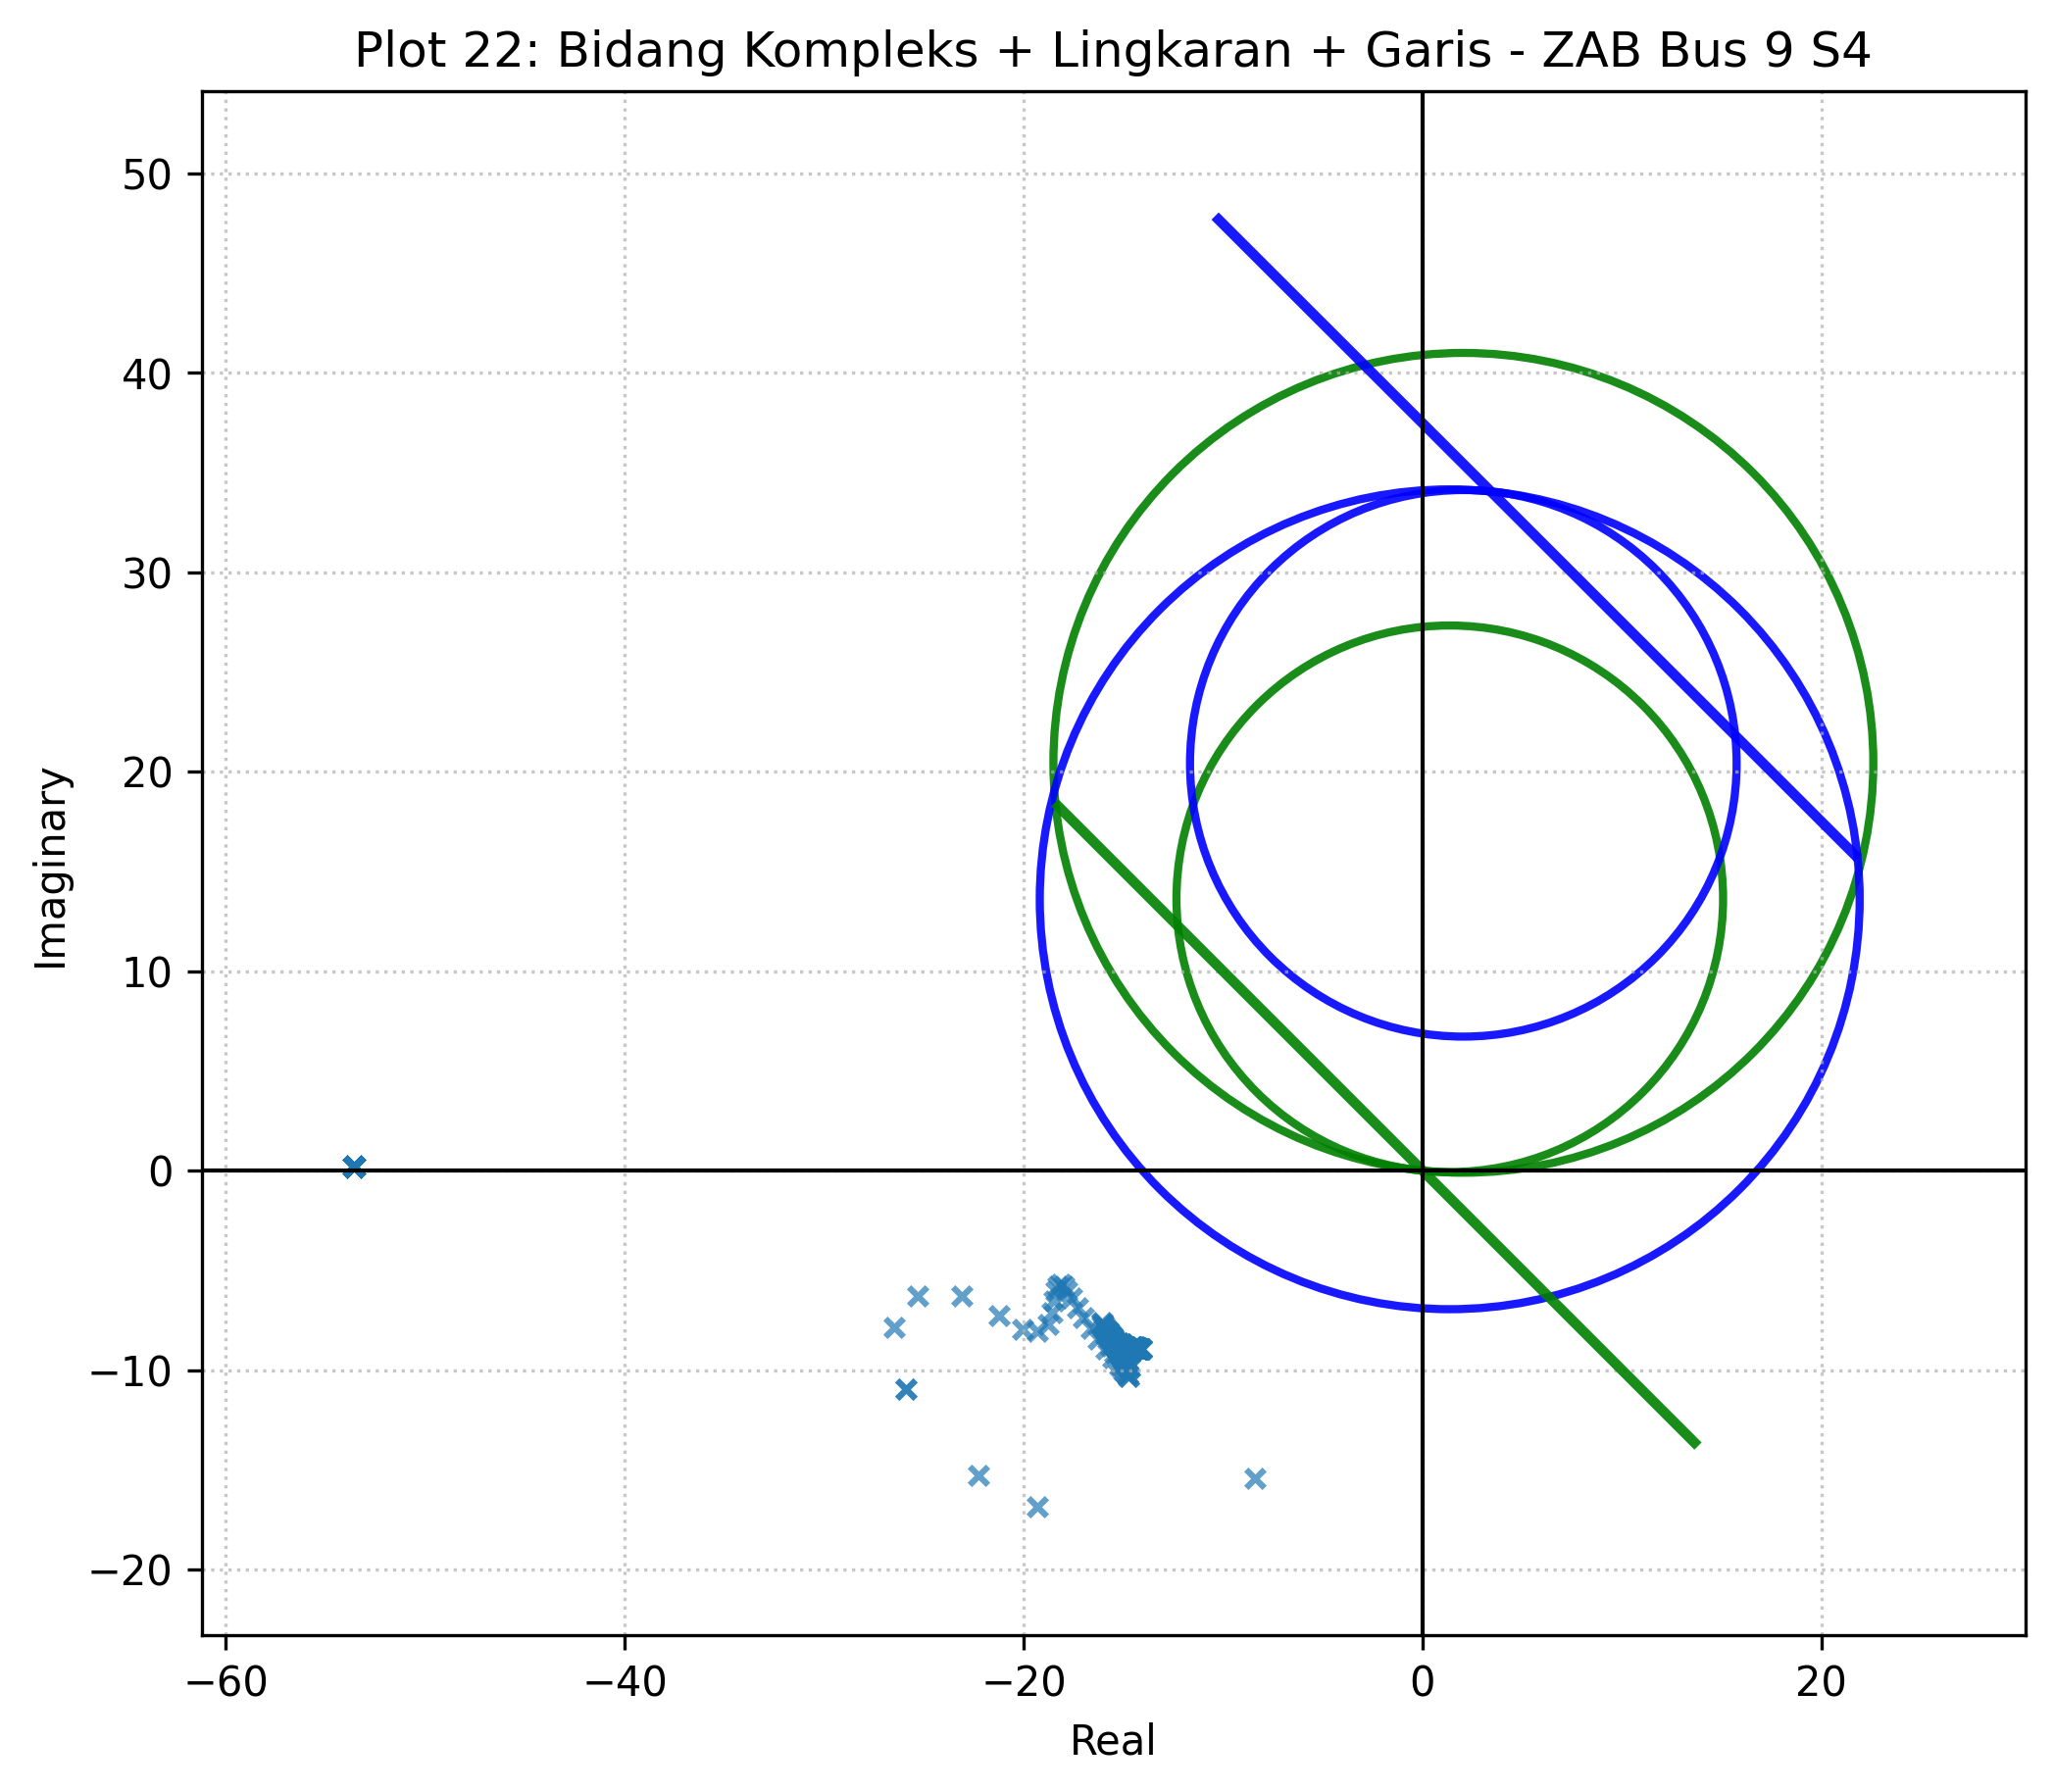
\includegraphics[width=0.8\textwidth]{contents/chapter-4/22_ZAB_Bus_9_S4_dengan_lingkaran_dan_garis.png}
%     \caption{Impedansi Tampak ZAB Bus 9 Skenario 4}
%     \label{fig:22_ZAB_Bus_9_S4_dengan_lingkaran_dan_garis}
% \end{figure}

% Terlihat pada gambar \ref{fig:22_ZAB_Bus_9_S4_dengan_lingkaran_dan_garis} bahwa impedansi tampak pada fasa A dengan fasa B yang dibaca oleh relay 21 sisi bus 9 saat terdapat gangguan bekerja dengan baik sesuai acuan pada \ref{subsec:tanpa_IBR_ex_3p} relay 21 bus 9 tidak mendeteksi adanya gangguan sehingga tidak mengirimkan sinyal trip kepada CB.

%%%%%%%%%%%%%%%%%%%%%%%%%%%%%%%%%SISI PRIMER%%%%%%%%%%%%%%%%%%%%%%%%%%%%%%%%%%

% \begin{figure}[H]
%     \centering
%     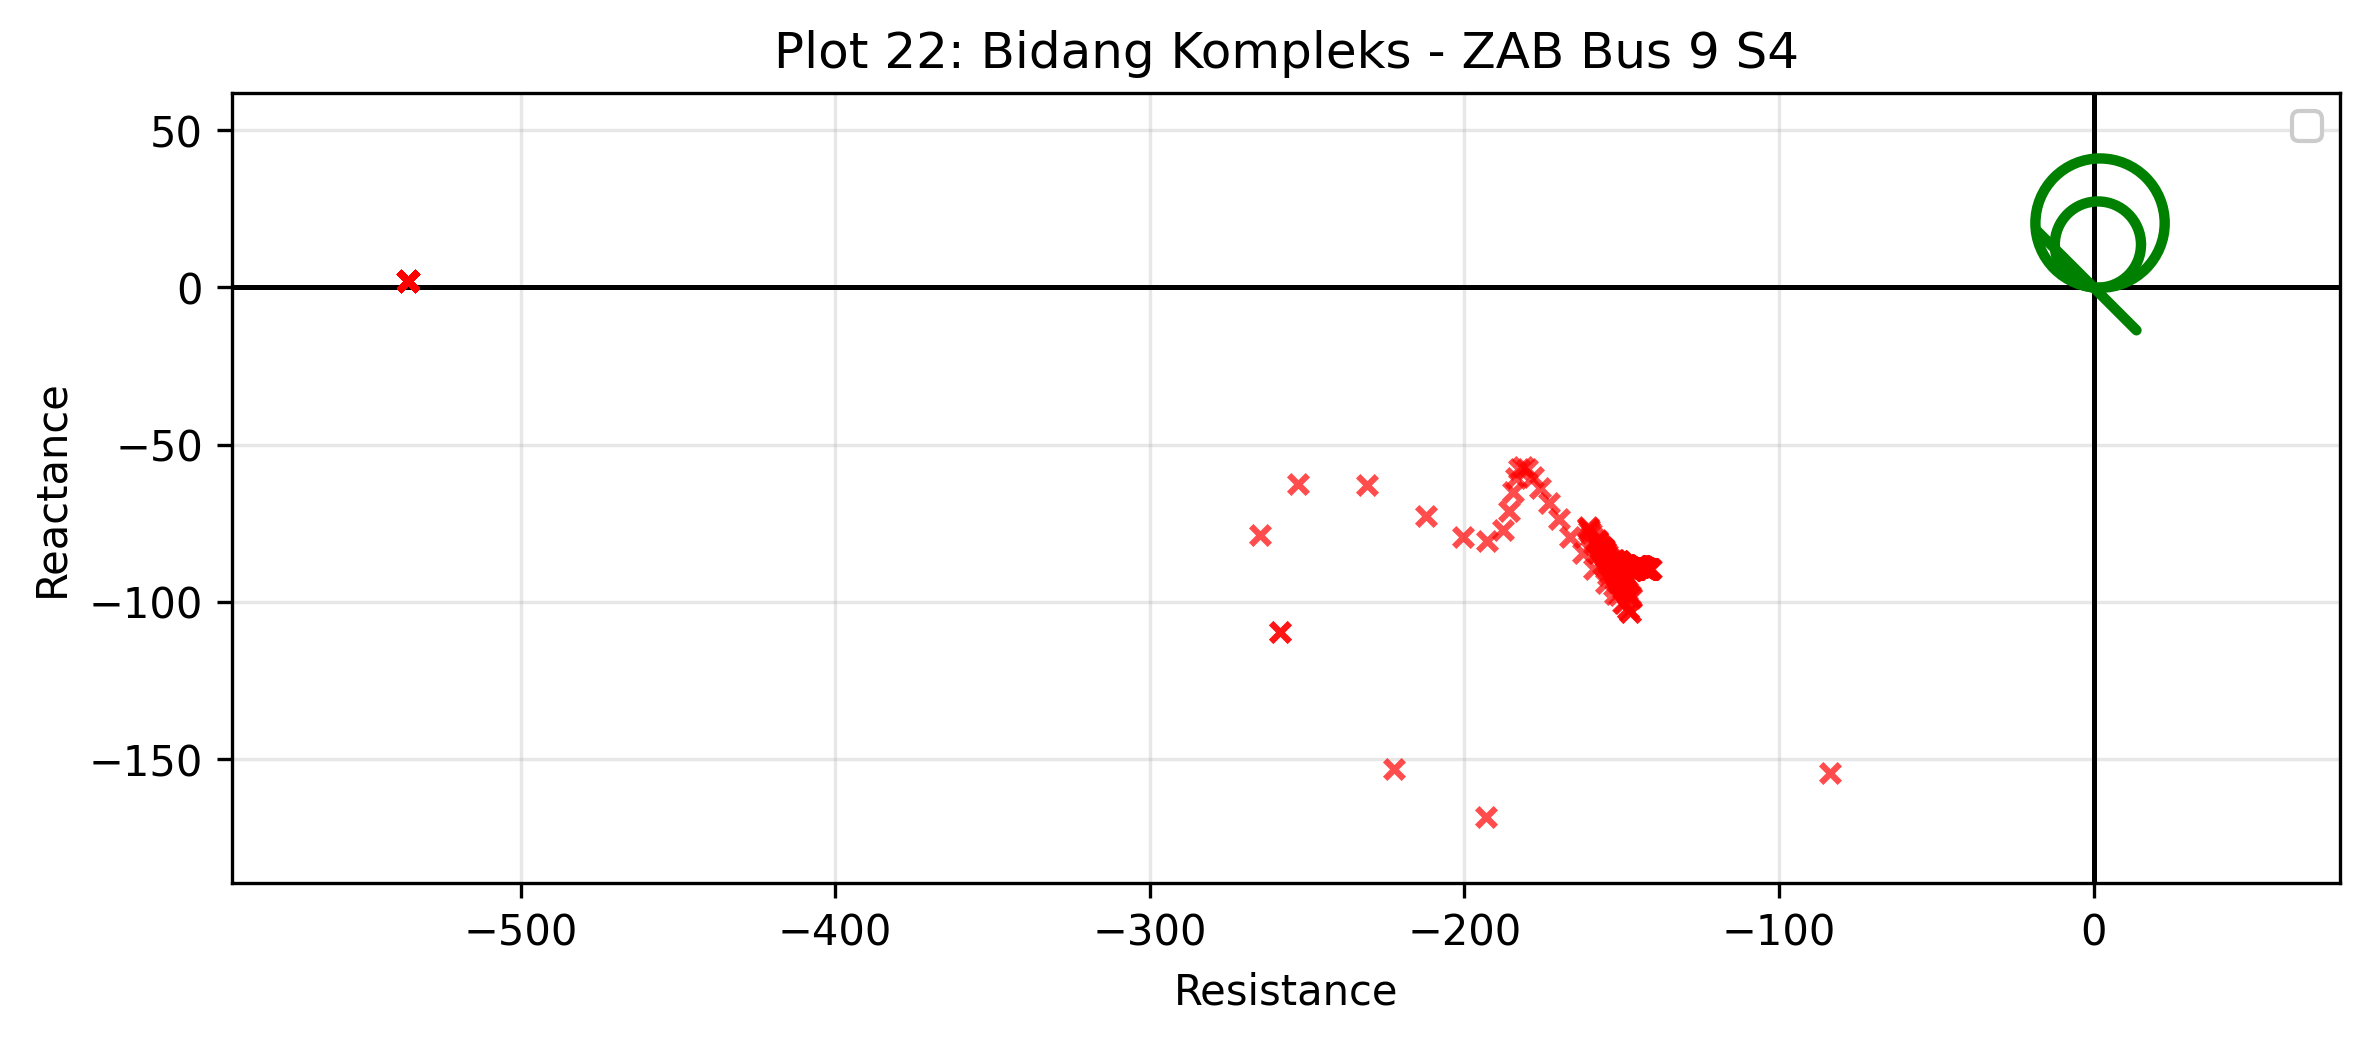
\includegraphics[width=0.8\textwidth]{contents/chapter-4/PRIA_22_ZAB_Bus_9_S4.png}
%     \caption{Impedansi Tampak ZAB Bus 9 Skenario 4}
%     \label{fig:PRIA_22_ZAB_Bus_9_S4}
% \end{figure}

% \begin{figure}[H]
%     \centering
%     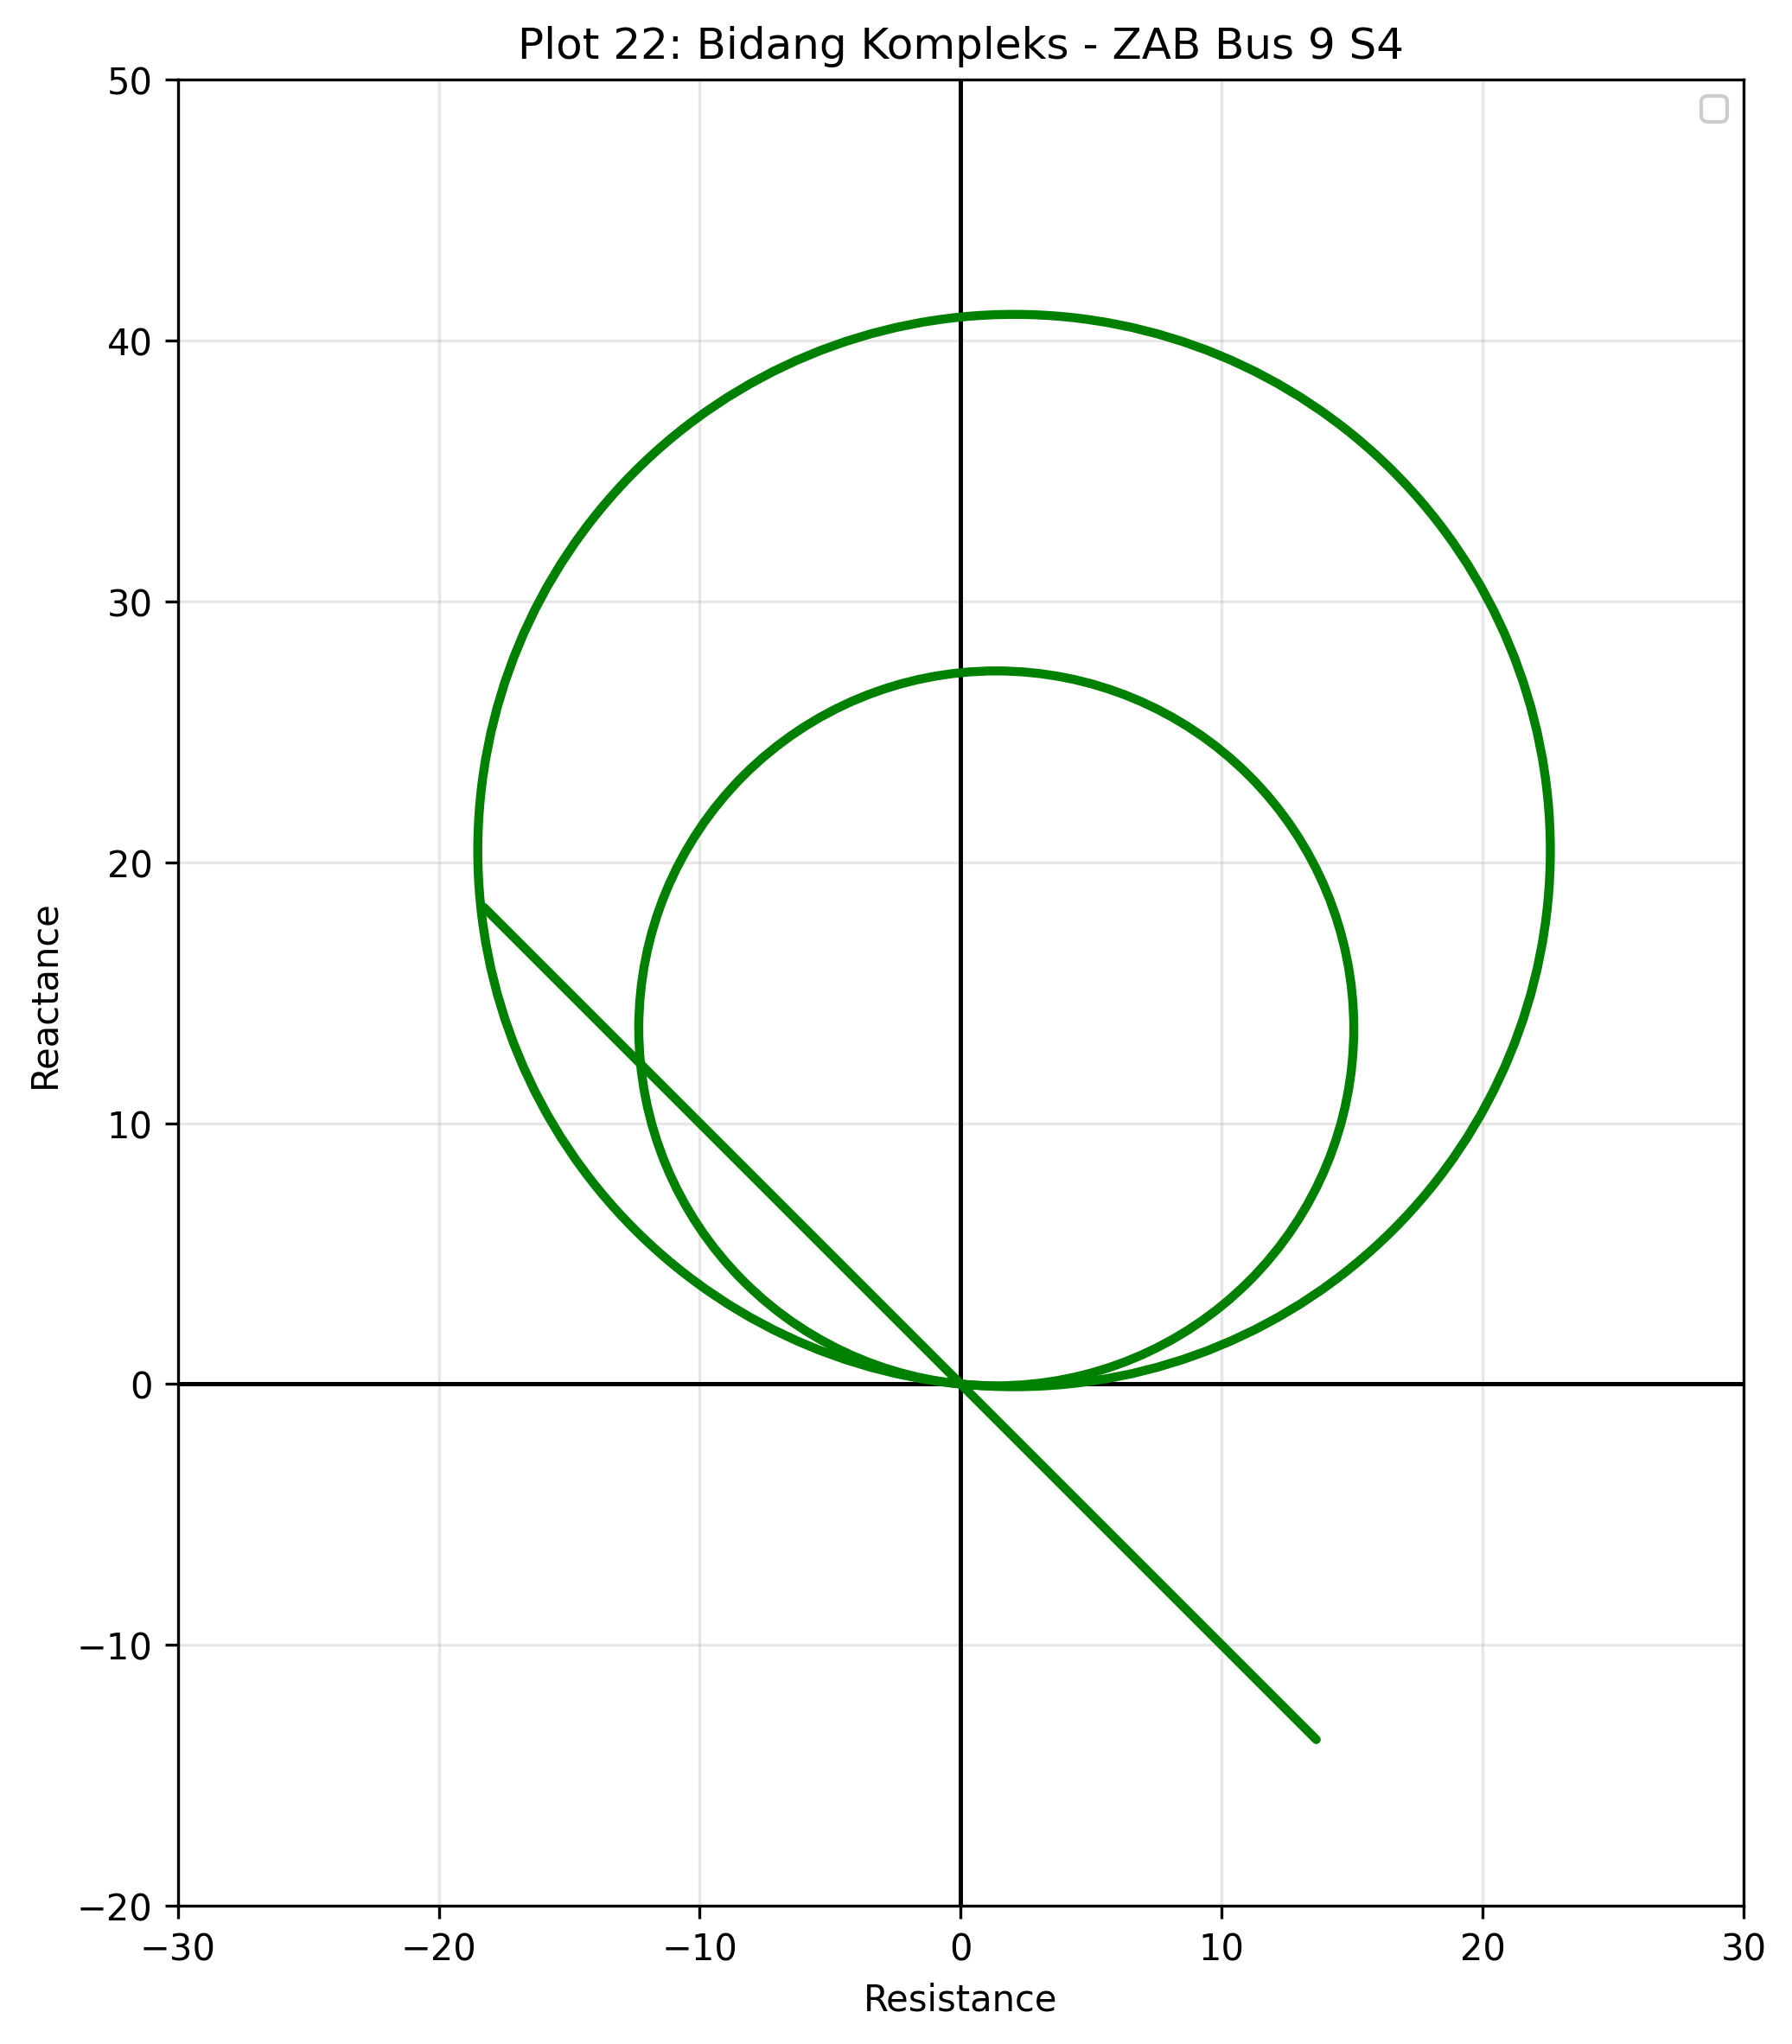
\includegraphics[width=0.8\textwidth]{contents/chapter-4/PRIZI_22_ZAB_Bus_9_S4.png}
%     \caption{Impedansi Tampak ZAB Bus 9 Skenario 4}
%     \label{fig:PRIZI_22_ZAB_Bus_9_S4}
% \end{figure}

\begin{figure}[H]
    \centering

    % Gambar sebelah kiri
    \begin{subfigure}[t]{0.48\textwidth}
        \centering
        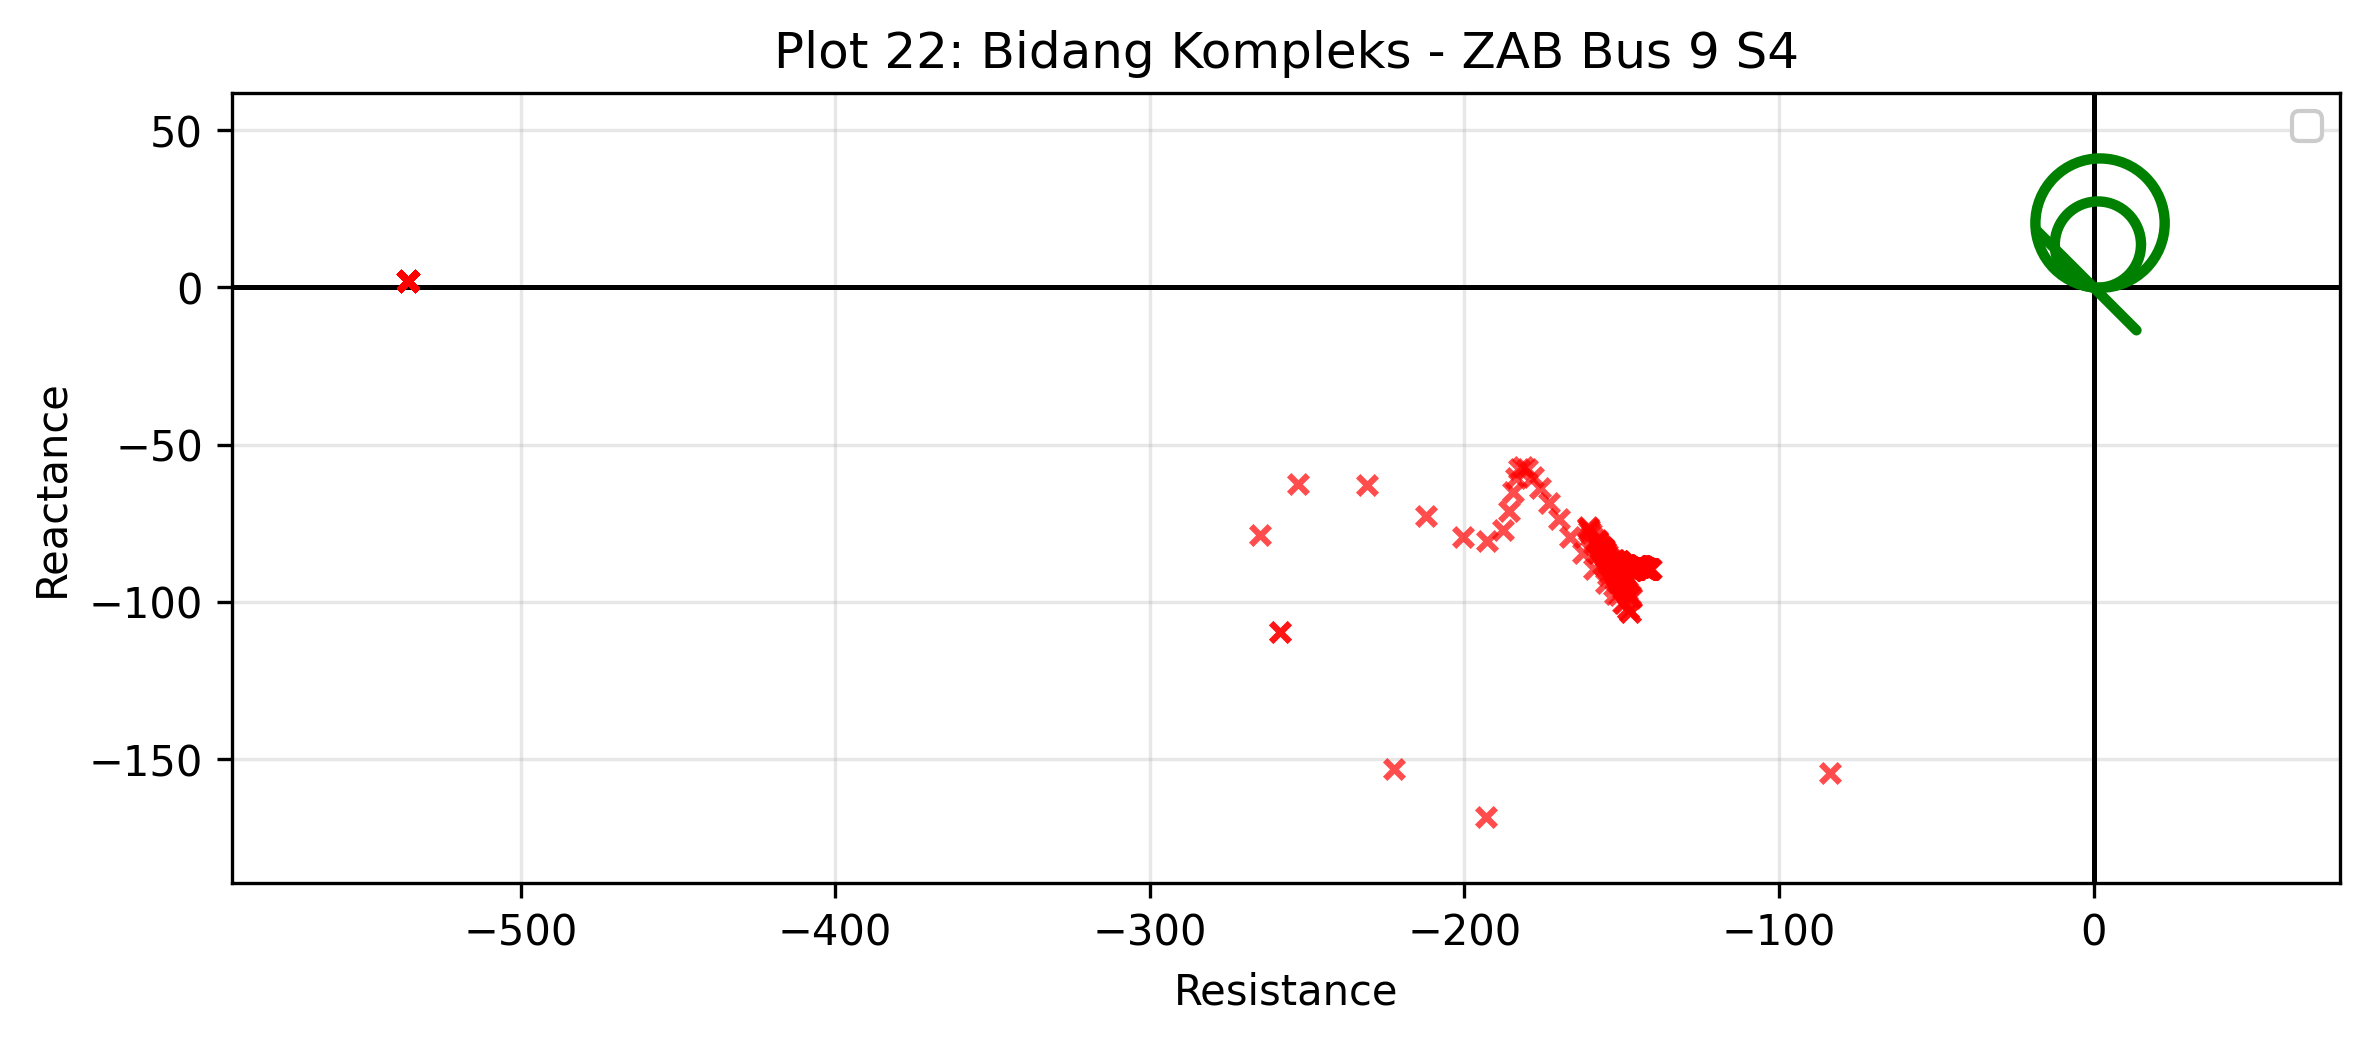
\includegraphics[width=\textwidth]{contents/chapter-4/PRIA_22_ZAB_Bus_9_S4.png}
        \caption{Seluruh Impedansi Tampak}
        \label{fig:PRIA_22_ZAB_Bus_9_S4}
    \end{subfigure}
    \hfill
    % Gambar sebelah kanan
    \begin{subfigure}[t]{0.48\textwidth}
        \centering
        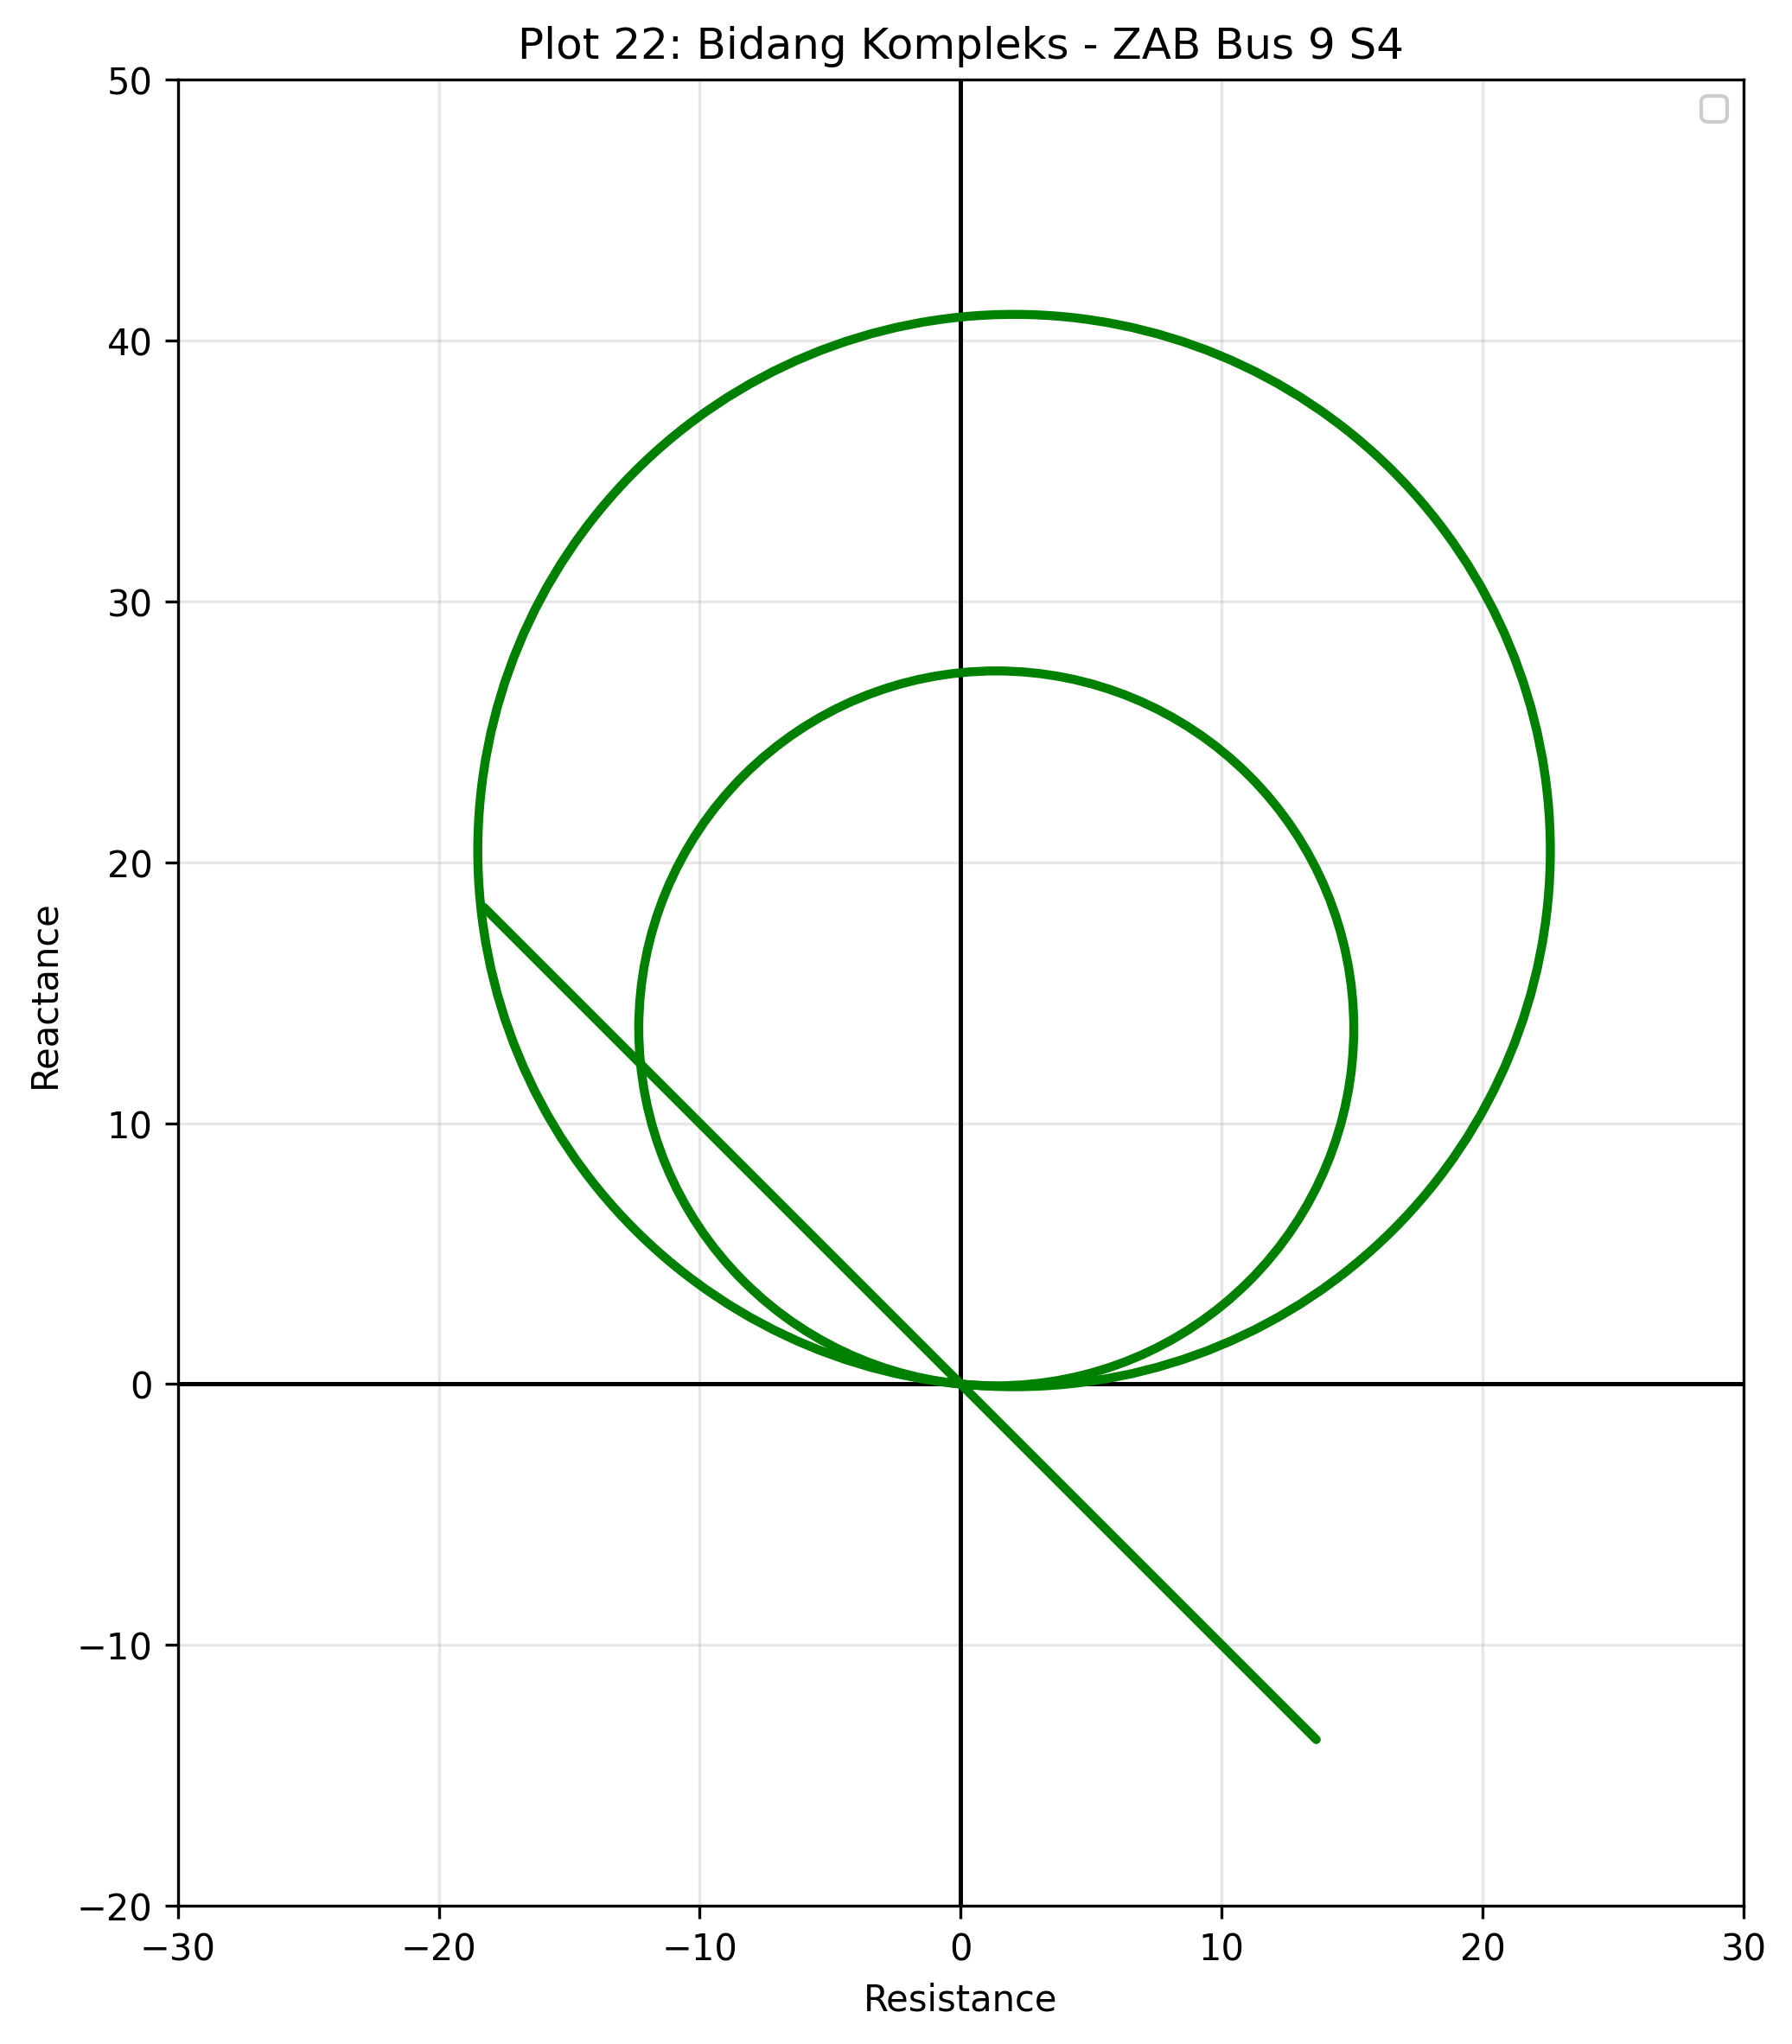
\includegraphics[width=\textwidth]{contents/chapter-4/PRIZI_22_ZAB_Bus_9_S4.png}
        \caption{Zoom In Pada Zona Proteksi}
        \label{fig:PRIZI_22_ZAB_Bus_9_S4}
    \end{subfigure}

    \caption{Impedansi Tampak ZAB Bus 9 Skenario 4}
    \label{fig:Impedansi_Tampak_ZAB_Bus_9_S4}
\end{figure}

Terlihat pada gambar \ref{fig:Impedansi_Tampak_ZAB_Bus_9_S4} bahwa impedansi tampak pada fasa A dengan fasa B yang dibaca oleh relay 21 sisi bus 9 saat terdapat gangguan bekerja dengan baik sesuai acuan pada \ref{subsec:tanpa_IBR_ex_3p} relay 21 bus 9 tidak mendeteksi adanya gangguan sehingga tidak mengirimkan sinyal trip kepada CB.

%%%%%%%%%%%%%%%%%%%%%%%%%%%%%%%%%%%%%%%%%%%%%%%%%%%%%%%%%%%%%%%

% \begin{figure}[H]
%     \centering
%     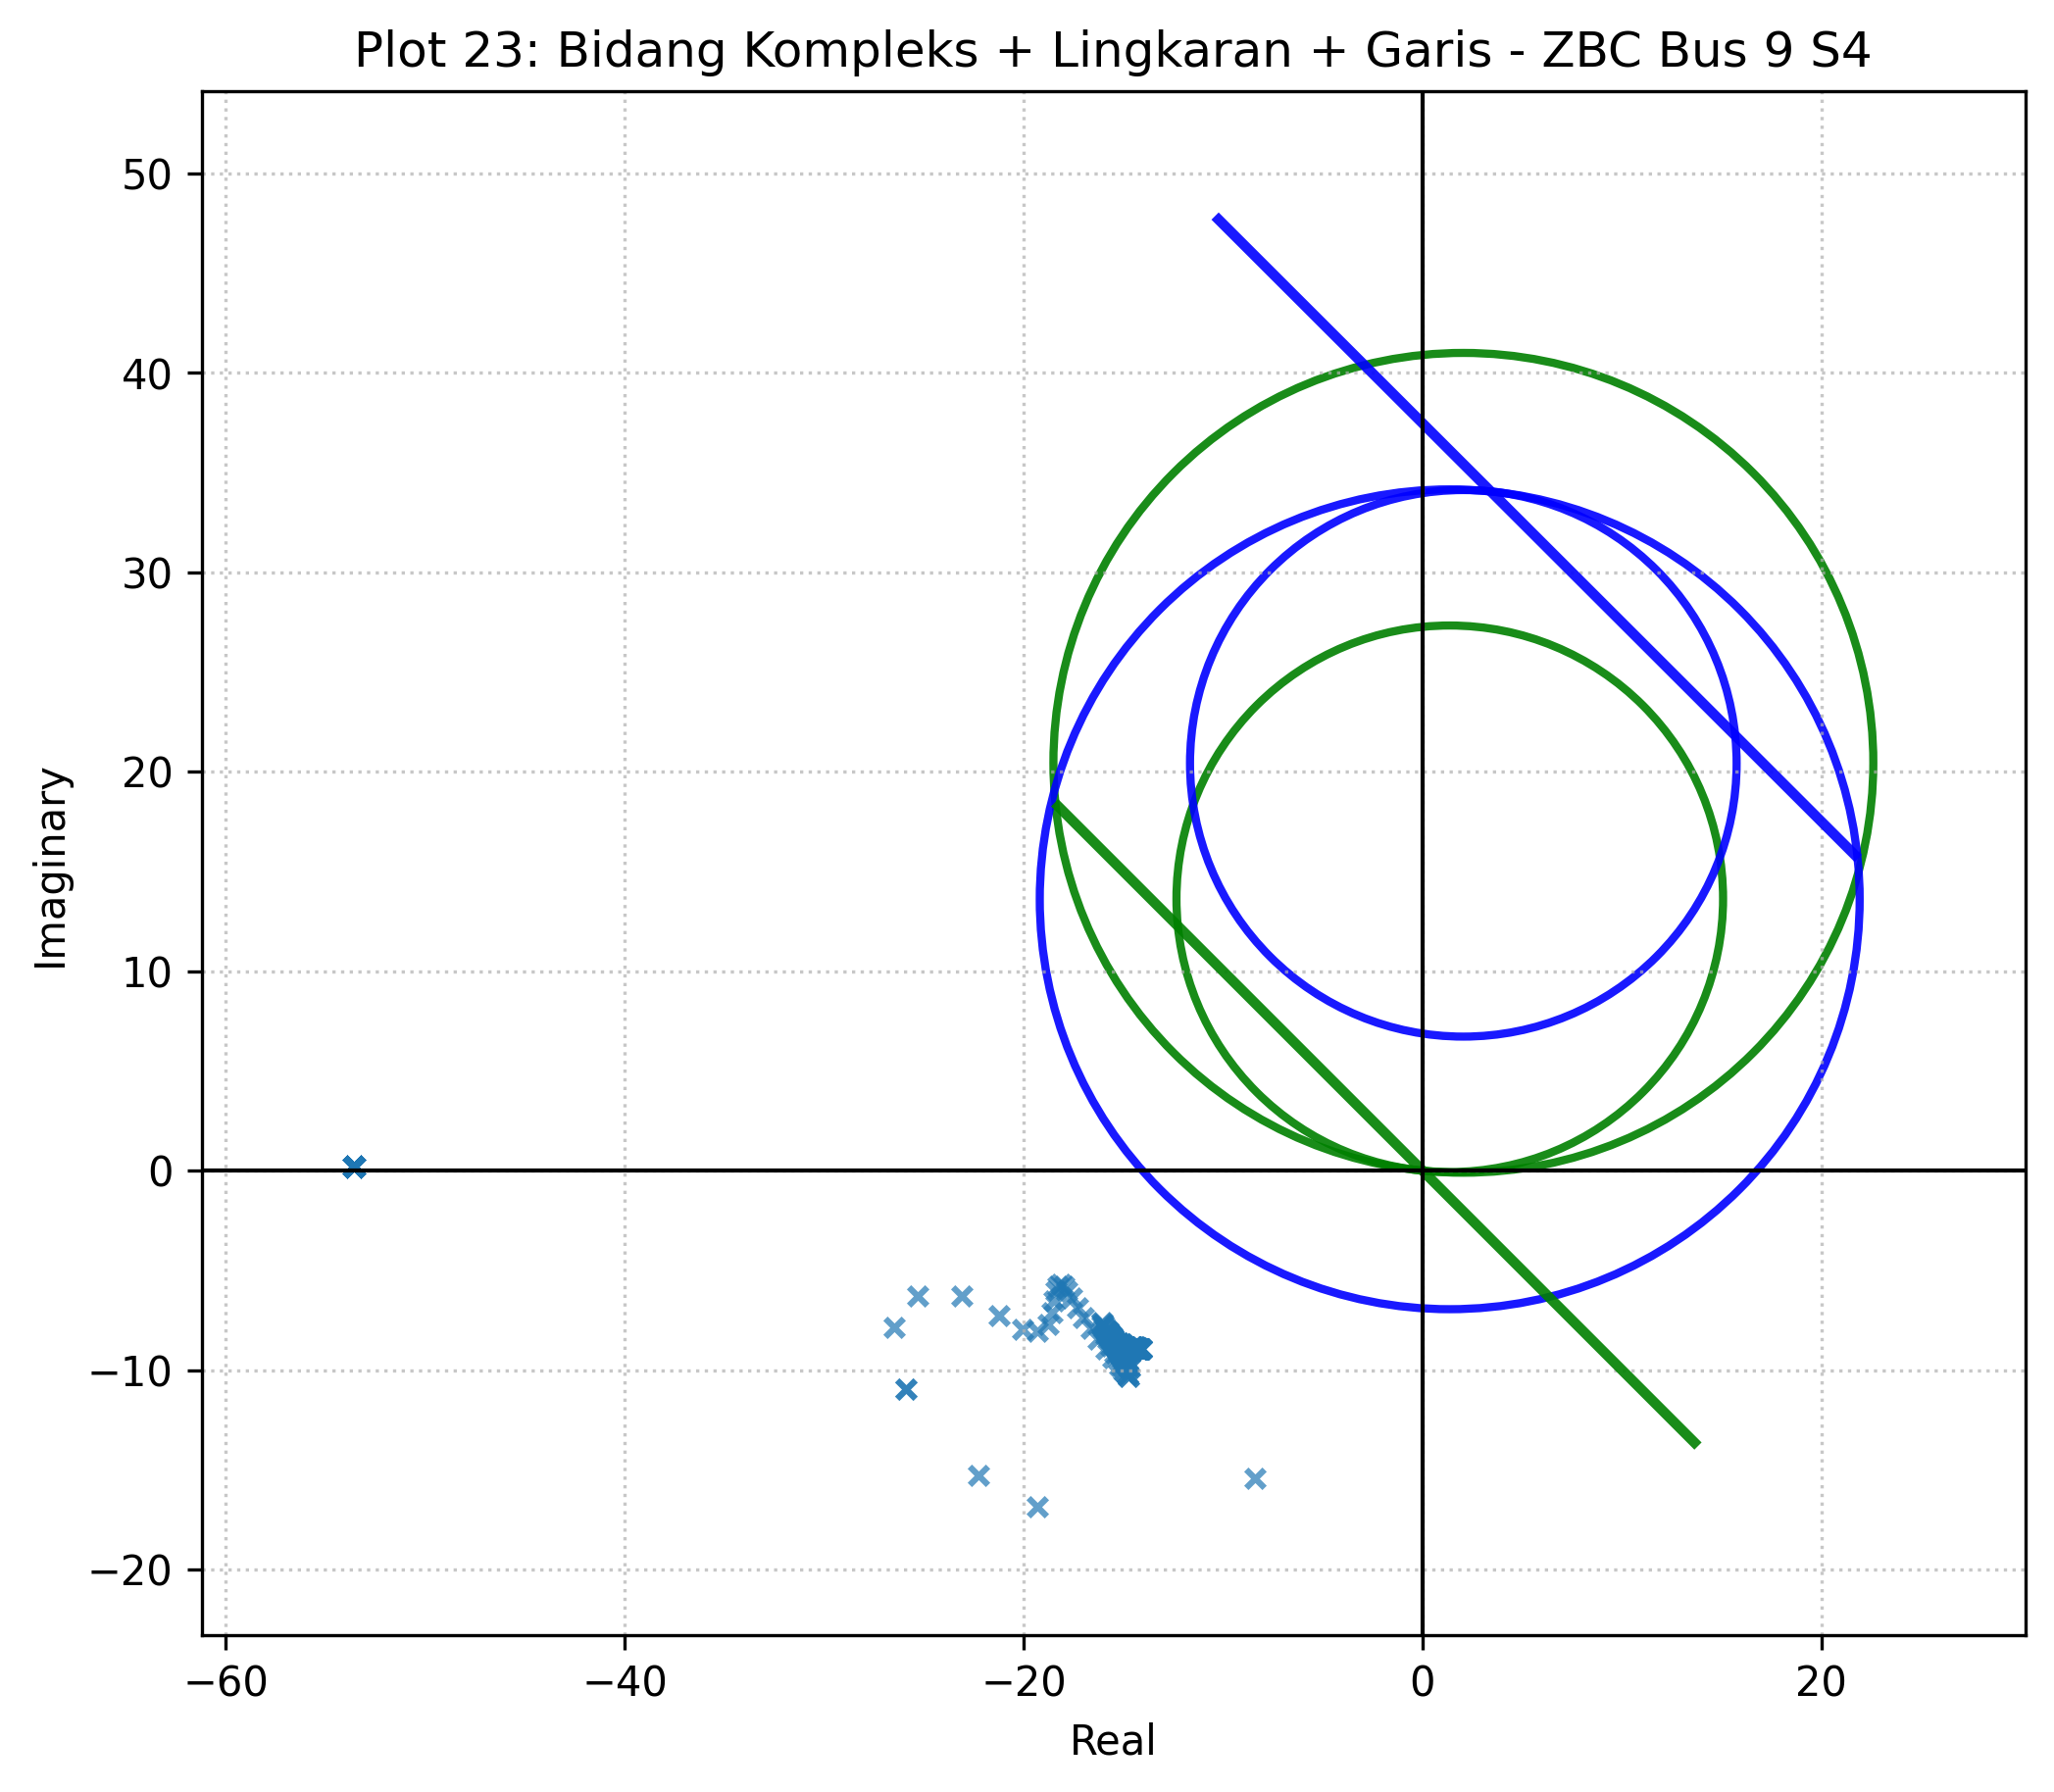
\includegraphics[width=0.8\textwidth]{contents/chapter-4/23_ZBC_Bus_9_S4_dengan_lingkaran_dan_garis.png}
%     \caption{Impedansi Tampak ZBC Bus 9 Skenario 4}
%     \label{fig:23_ZBC_Bus_9_S4_dengan_lingkaran_dan_garis}
% \end{figure}

% Terlihat pada gambar \ref{fig:23_ZBC_Bus_9_S4_dengan_lingkaran_dan_garis} bahwa impedansi tampak pada fasa B dengan fasa C yang dibaca oleh relay 21 sisi bus 9 saat terdapat gangguan bekerja dengan baik sesuai acuan pada \ref{subsec:tanpa_IBR_ex_3p} relay 21 bus 9 tidak mendeteksi adanya gangguan sehingga tidak mengirimkan sinyal trip kepada CB.

%%%%%%%%%%%%%%%%%%%%%%%%%%%%%%%%%SISI PRIMER%%%%%%%%%%%%%%%%%%%%%%%%%%%%%%%%%%

% \begin{figure}[H]
%     \centering
%     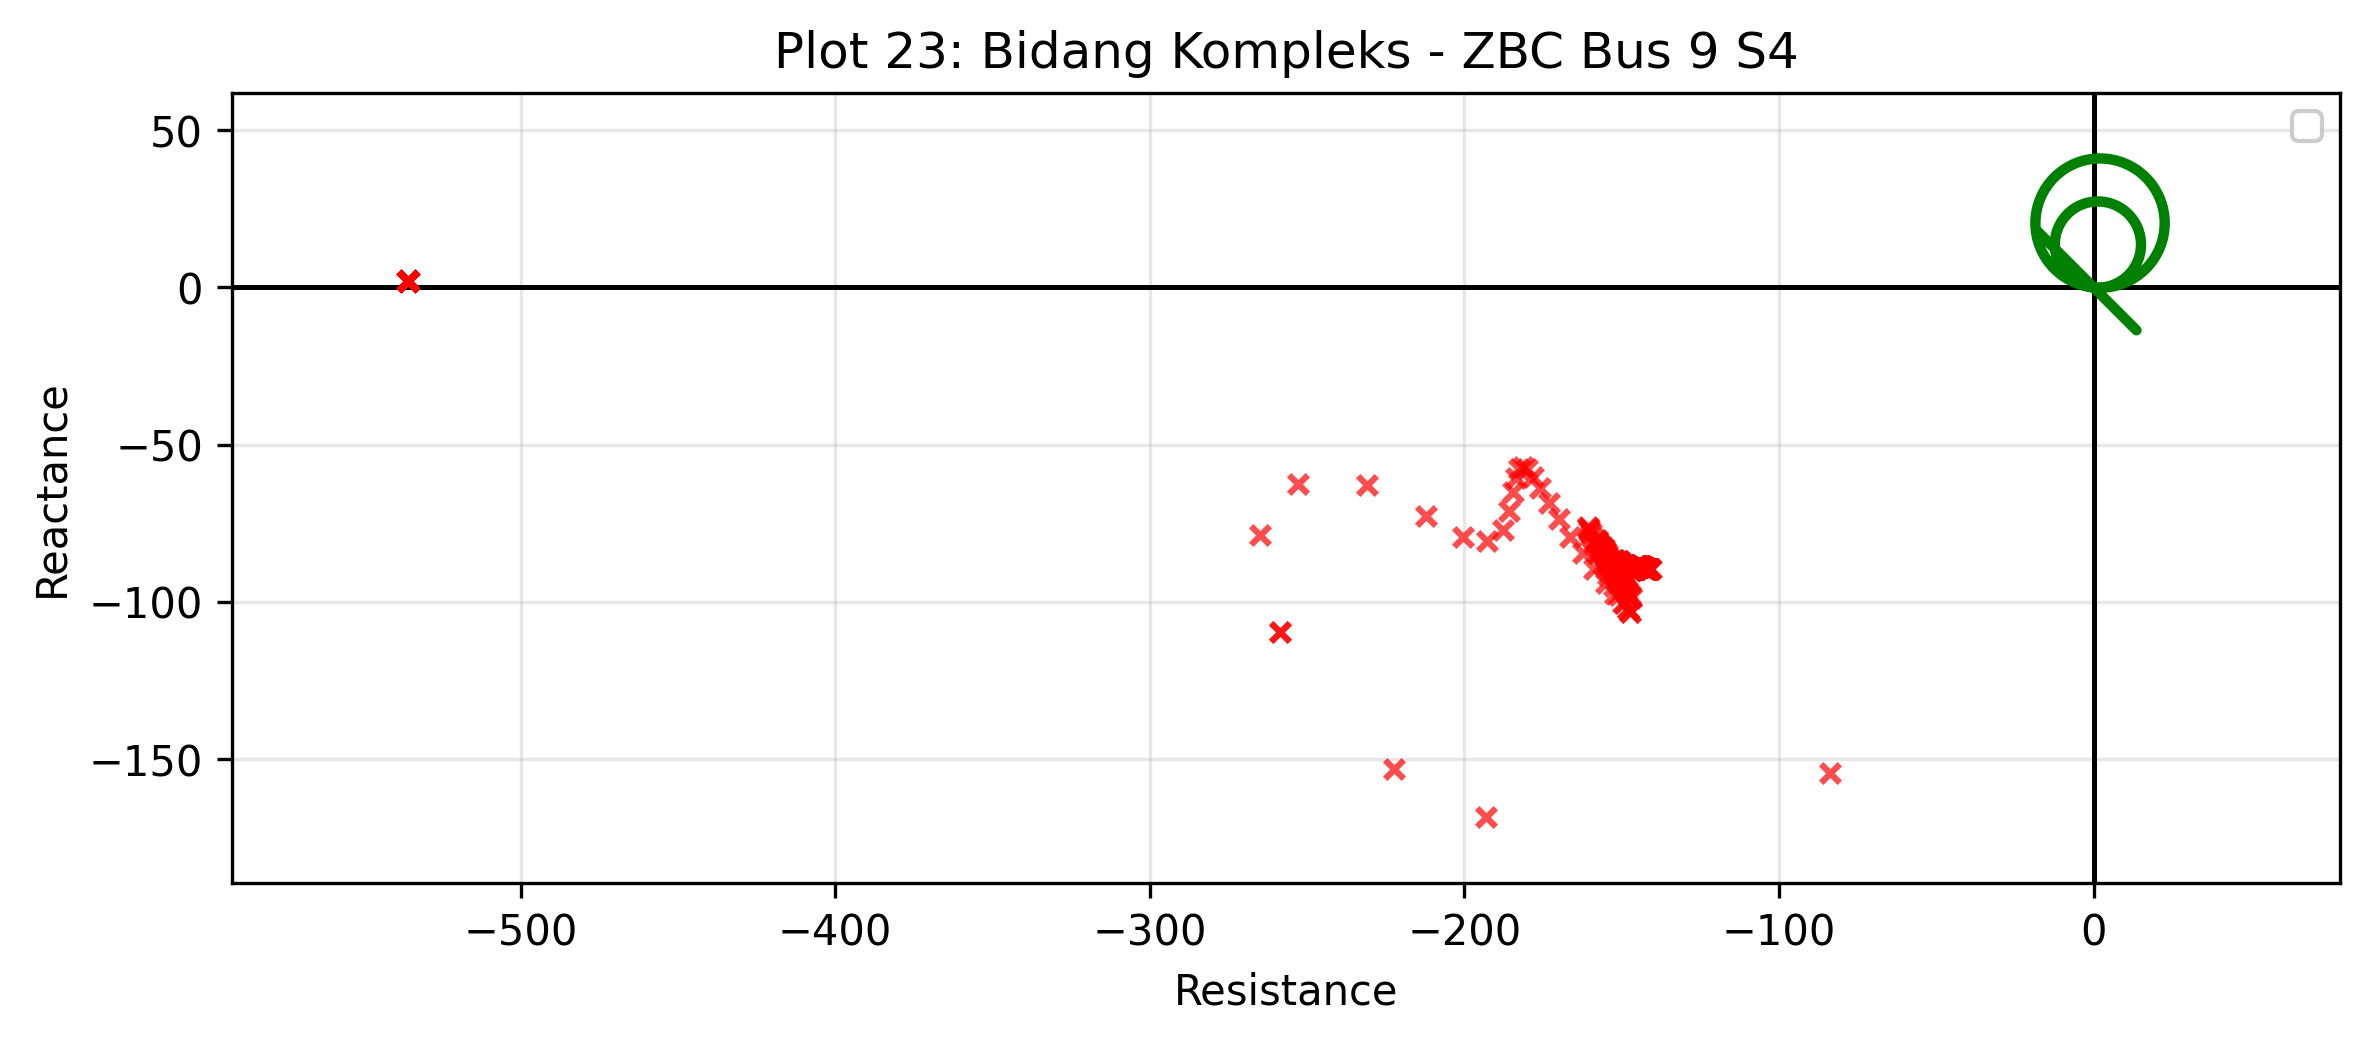
\includegraphics[width=0.8\textwidth]{contents/chapter-4/PRIA_23_ZBC_Bus_9_S4.png}
%     \caption{Impedansi Tampak ZBC Bus 9 Skenario 4}
%     \label{fig:PRIA_23_ZBC_Bus_9_S4}
% \end{figure}

% \begin{figure}[H]
%     \centering
%     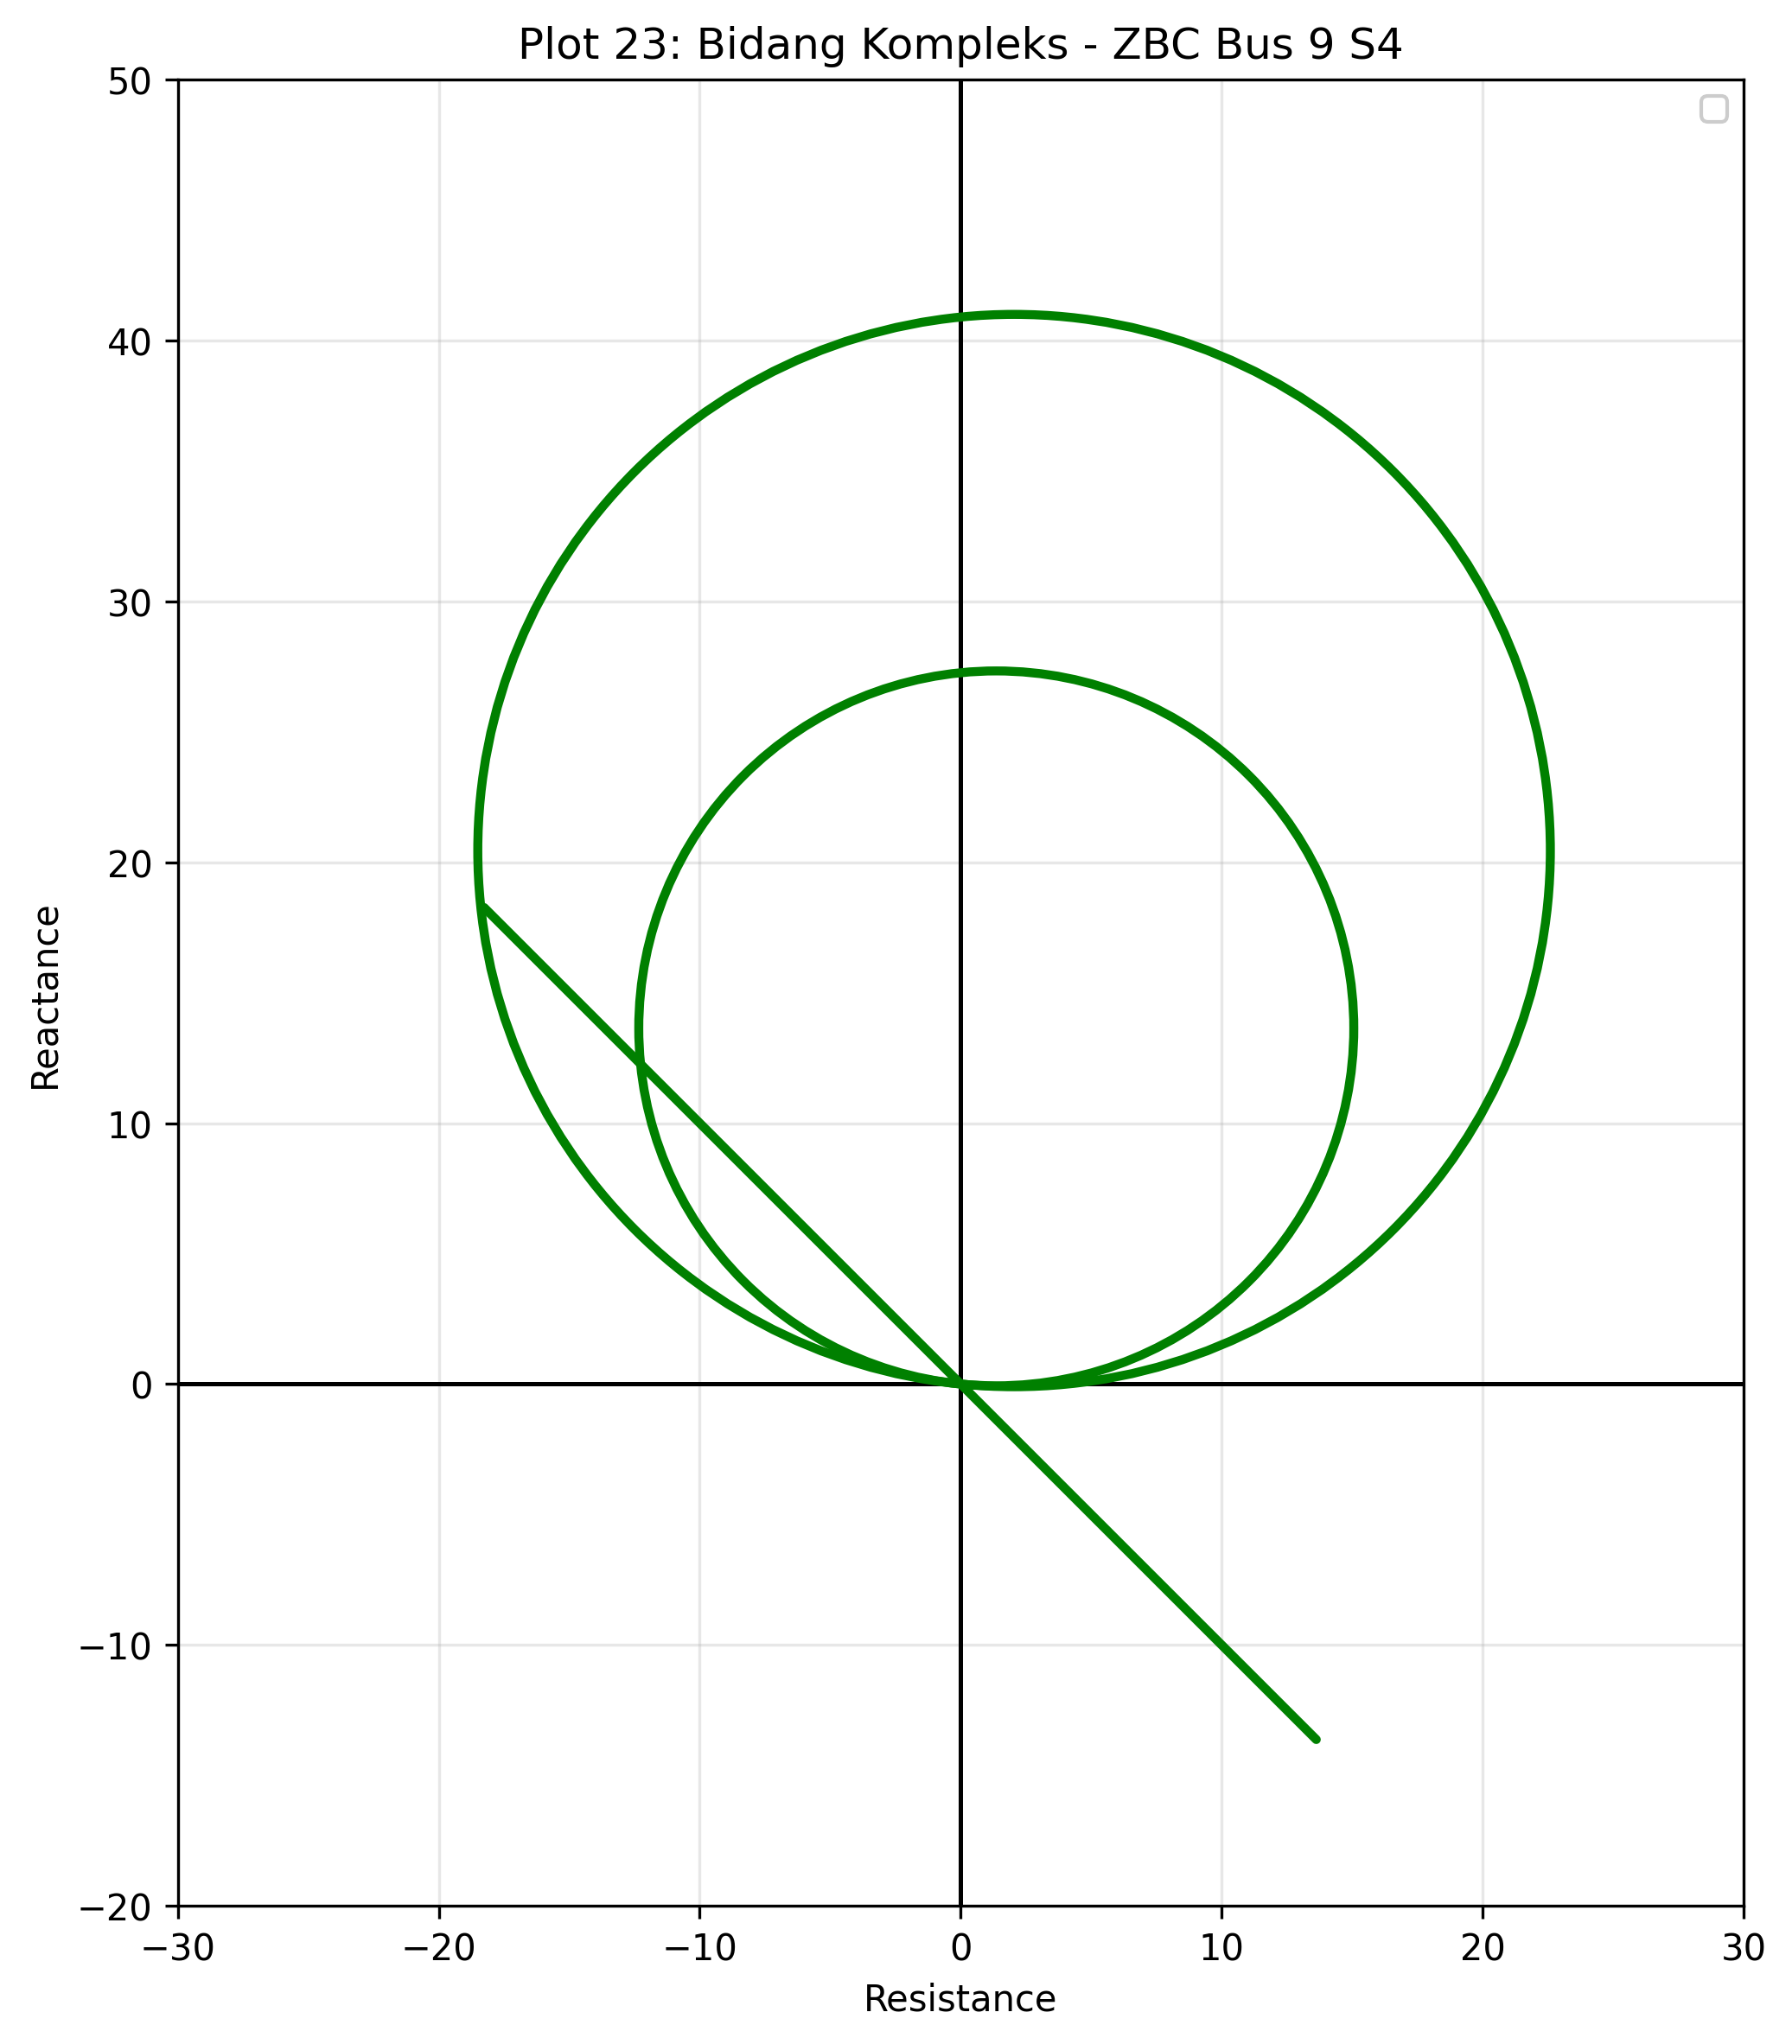
\includegraphics[width=0.8\textwidth]{contents/chapter-4/PRIZI_23_ZBC_Bus_9_S4.png}
%     \caption{Impedansi Tampak ZBC Bus 9 Skenario 4}
%     \label{fig:PRIZI_23_ZBC_Bus_9_S4}
% \end{figure}

\begin{figure}[H]
    \centering

    % Gambar sebelah kiri
    \begin{subfigure}[t]{0.48\textwidth}
        \centering
        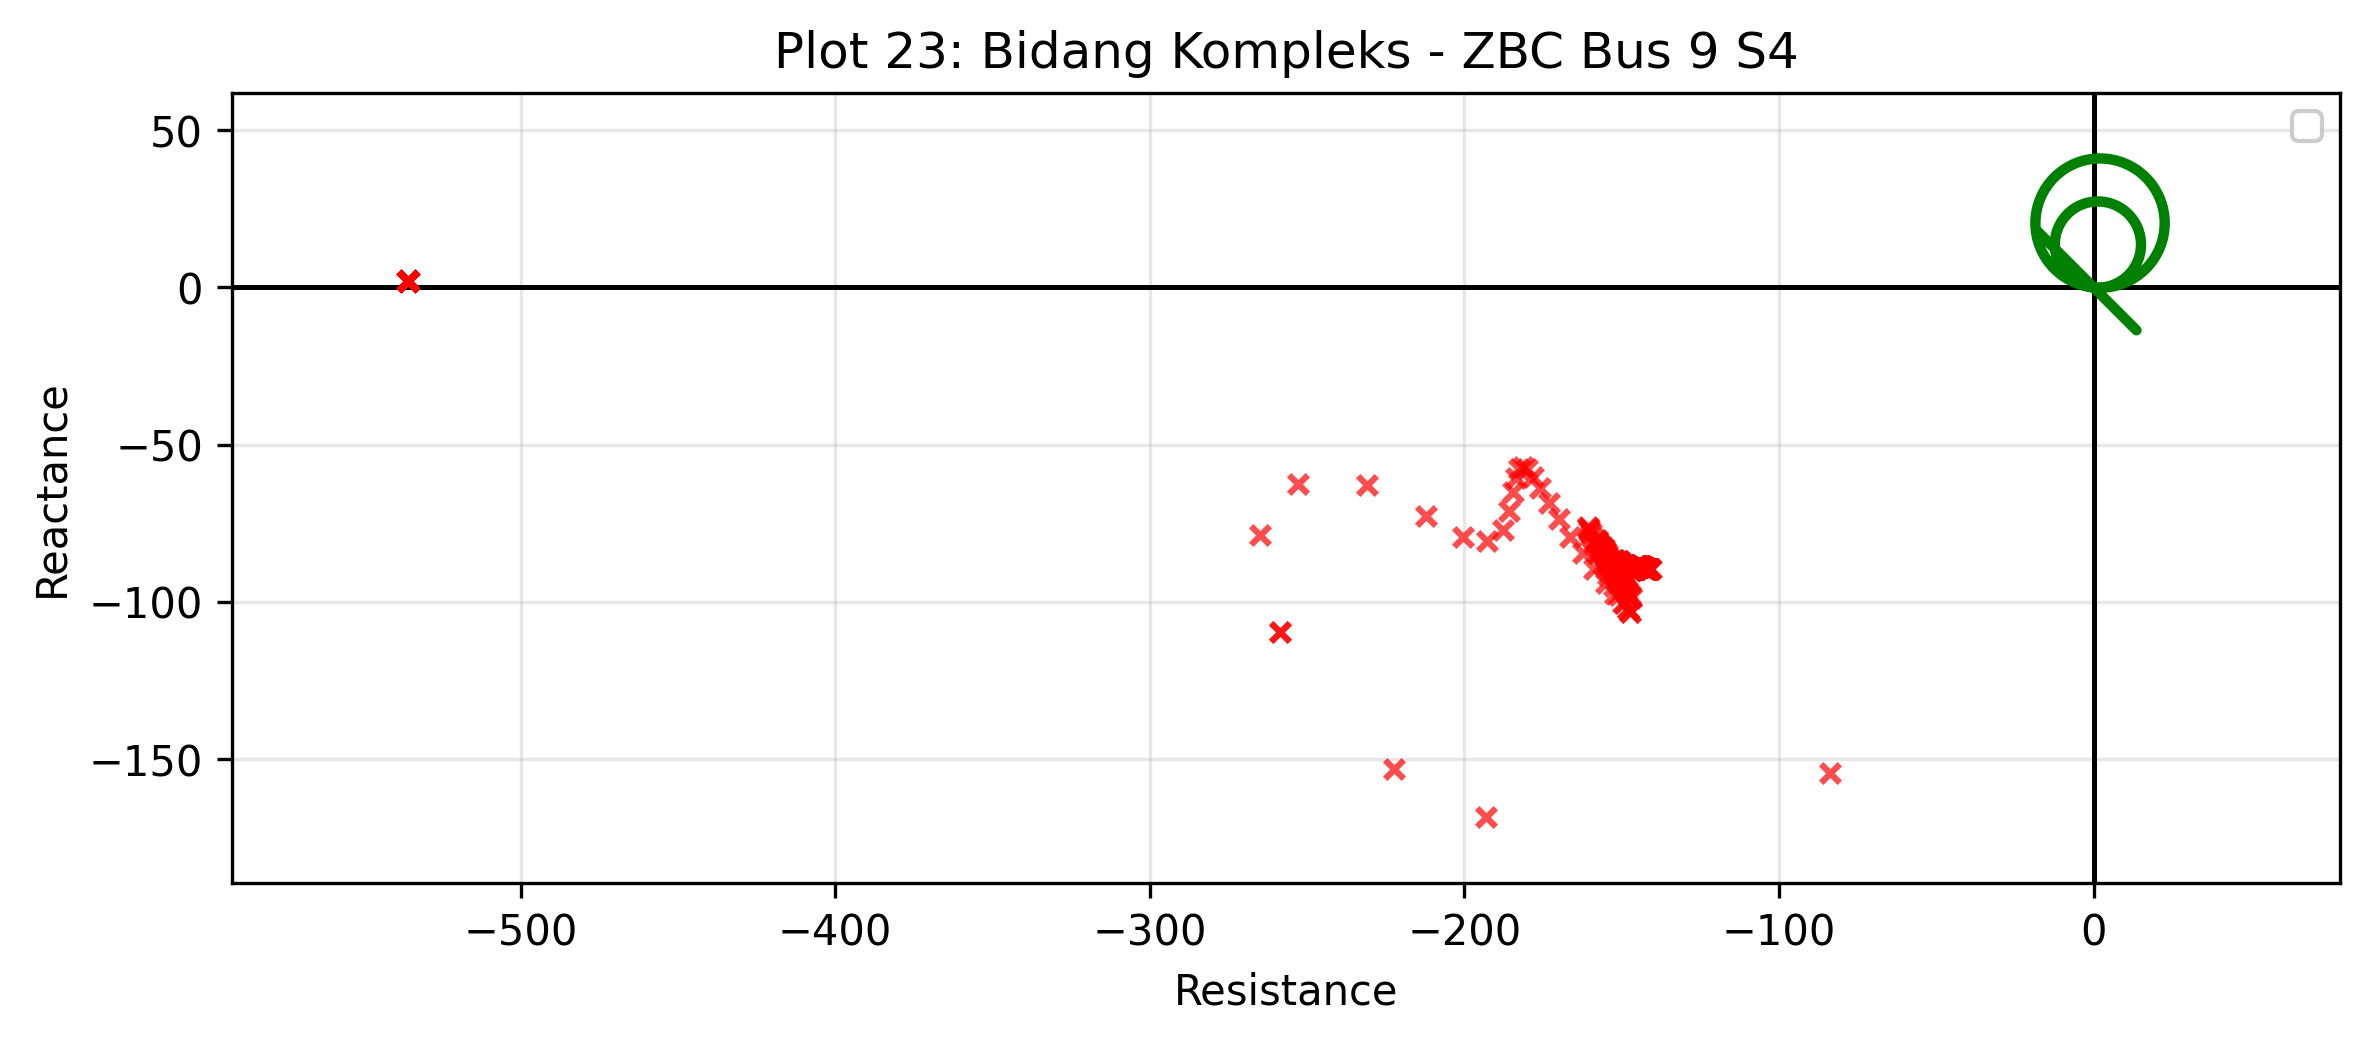
\includegraphics[width=\textwidth]{contents/chapter-4/PRIA_23_ZBC_Bus_9_S4.png}
        \caption{Seluruh Impedansi Tampak}
        \label{fig:PRIA_23_ZBC_Bus_9_S4}
    \end{subfigure}
    \hfill
    % Gambar sebelah kanan
    \begin{subfigure}[t]{0.48\textwidth}
        \centering
        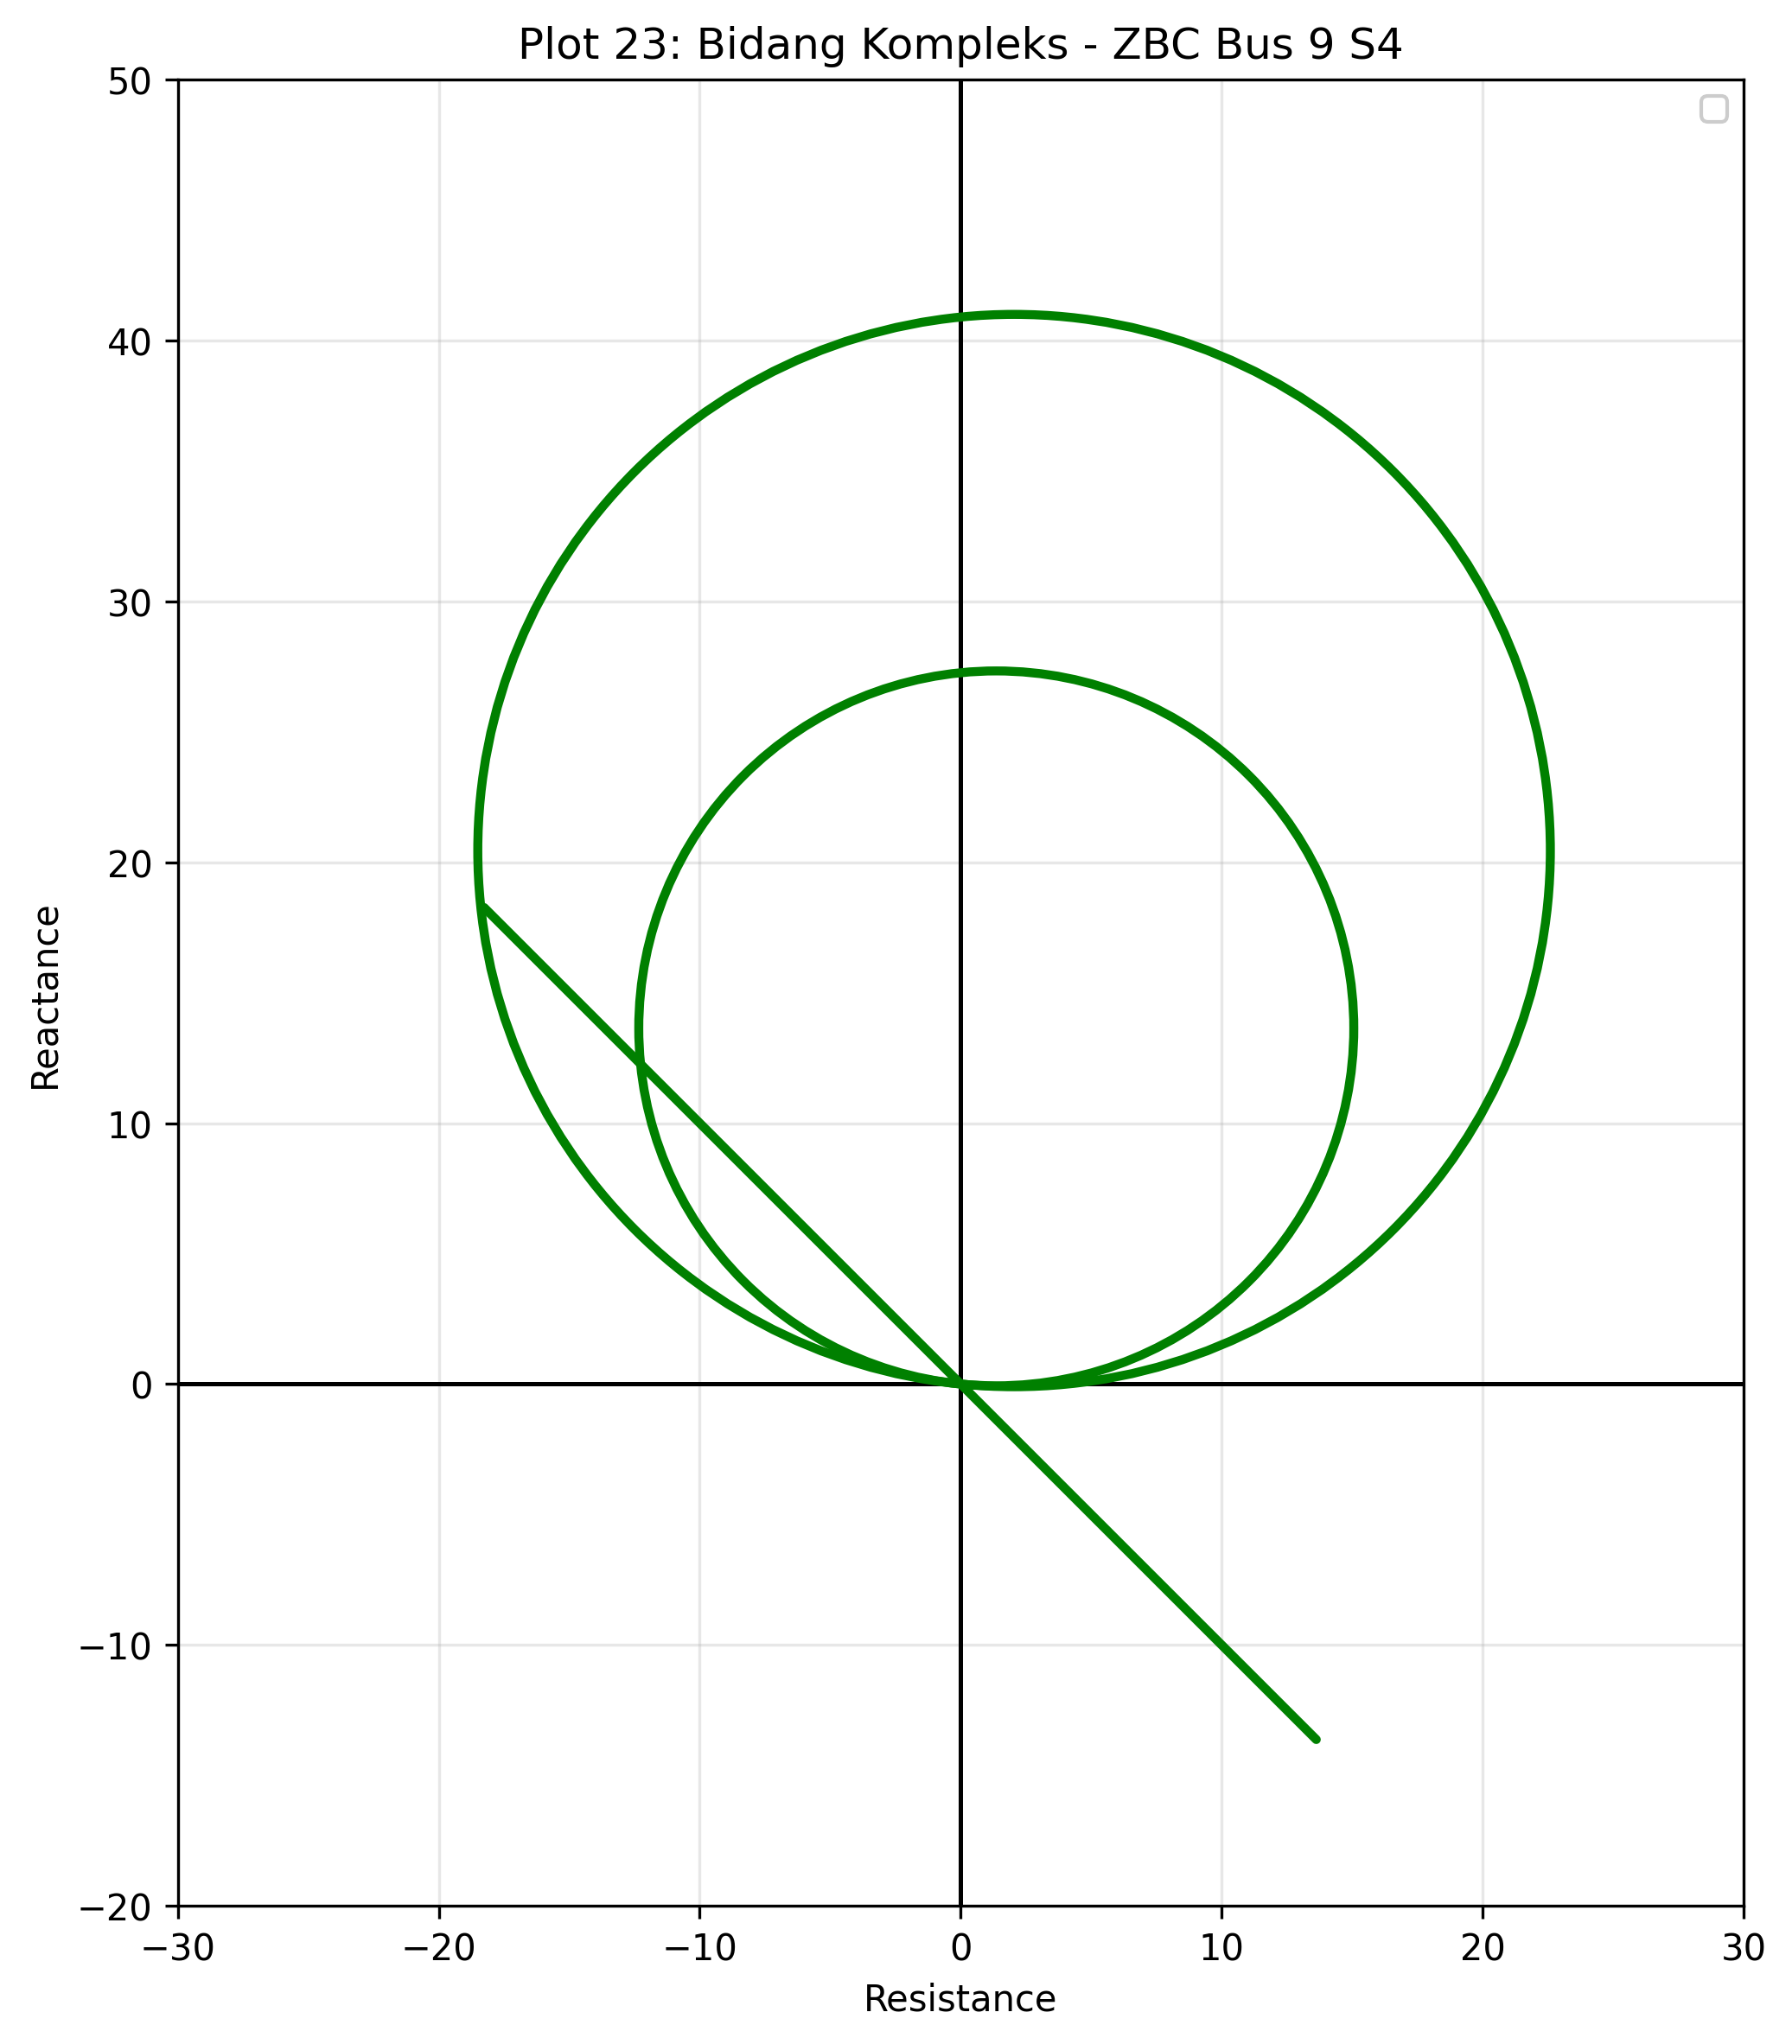
\includegraphics[width=\textwidth]{contents/chapter-4/PRIZI_23_ZBC_Bus_9_S4.png}
        \caption{Zoom In Pada Zona Proteksi}
        \label{fig:PRIZI_23_ZBC_Bus_9_S4}
    \end{subfigure}

    \caption{Impedansi Tampak ZBC Bus 9 Skenario 4}
    \label{fig:Impedansi_Tampak_ZBC_Bus_9_S4}
\end{figure}

Terlihat pada gambar \ref{fig:Impedansi_Tampak_ZBC_Bus_9_S4} bahwa impedansi tampak pada fasa B dengan fasa C yang dibaca oleh relay 21 sisi bus 9 saat terdapat gangguan bekerja dengan baik sesuai acuan pada \ref{subsec:tanpa_IBR_ex_3p} relay 21 bus 9 tidak mendeteksi adanya gangguan sehingga tidak mengirimkan sinyal trip kepada CB.

%%%%%%%%%%%%%%%%%%%%%%%%%%%%%%%%%%%%%%%%%%%%%%%%%%%%%%%%%%%%%%%

% \begin{figure}[H]
%     \centering
%     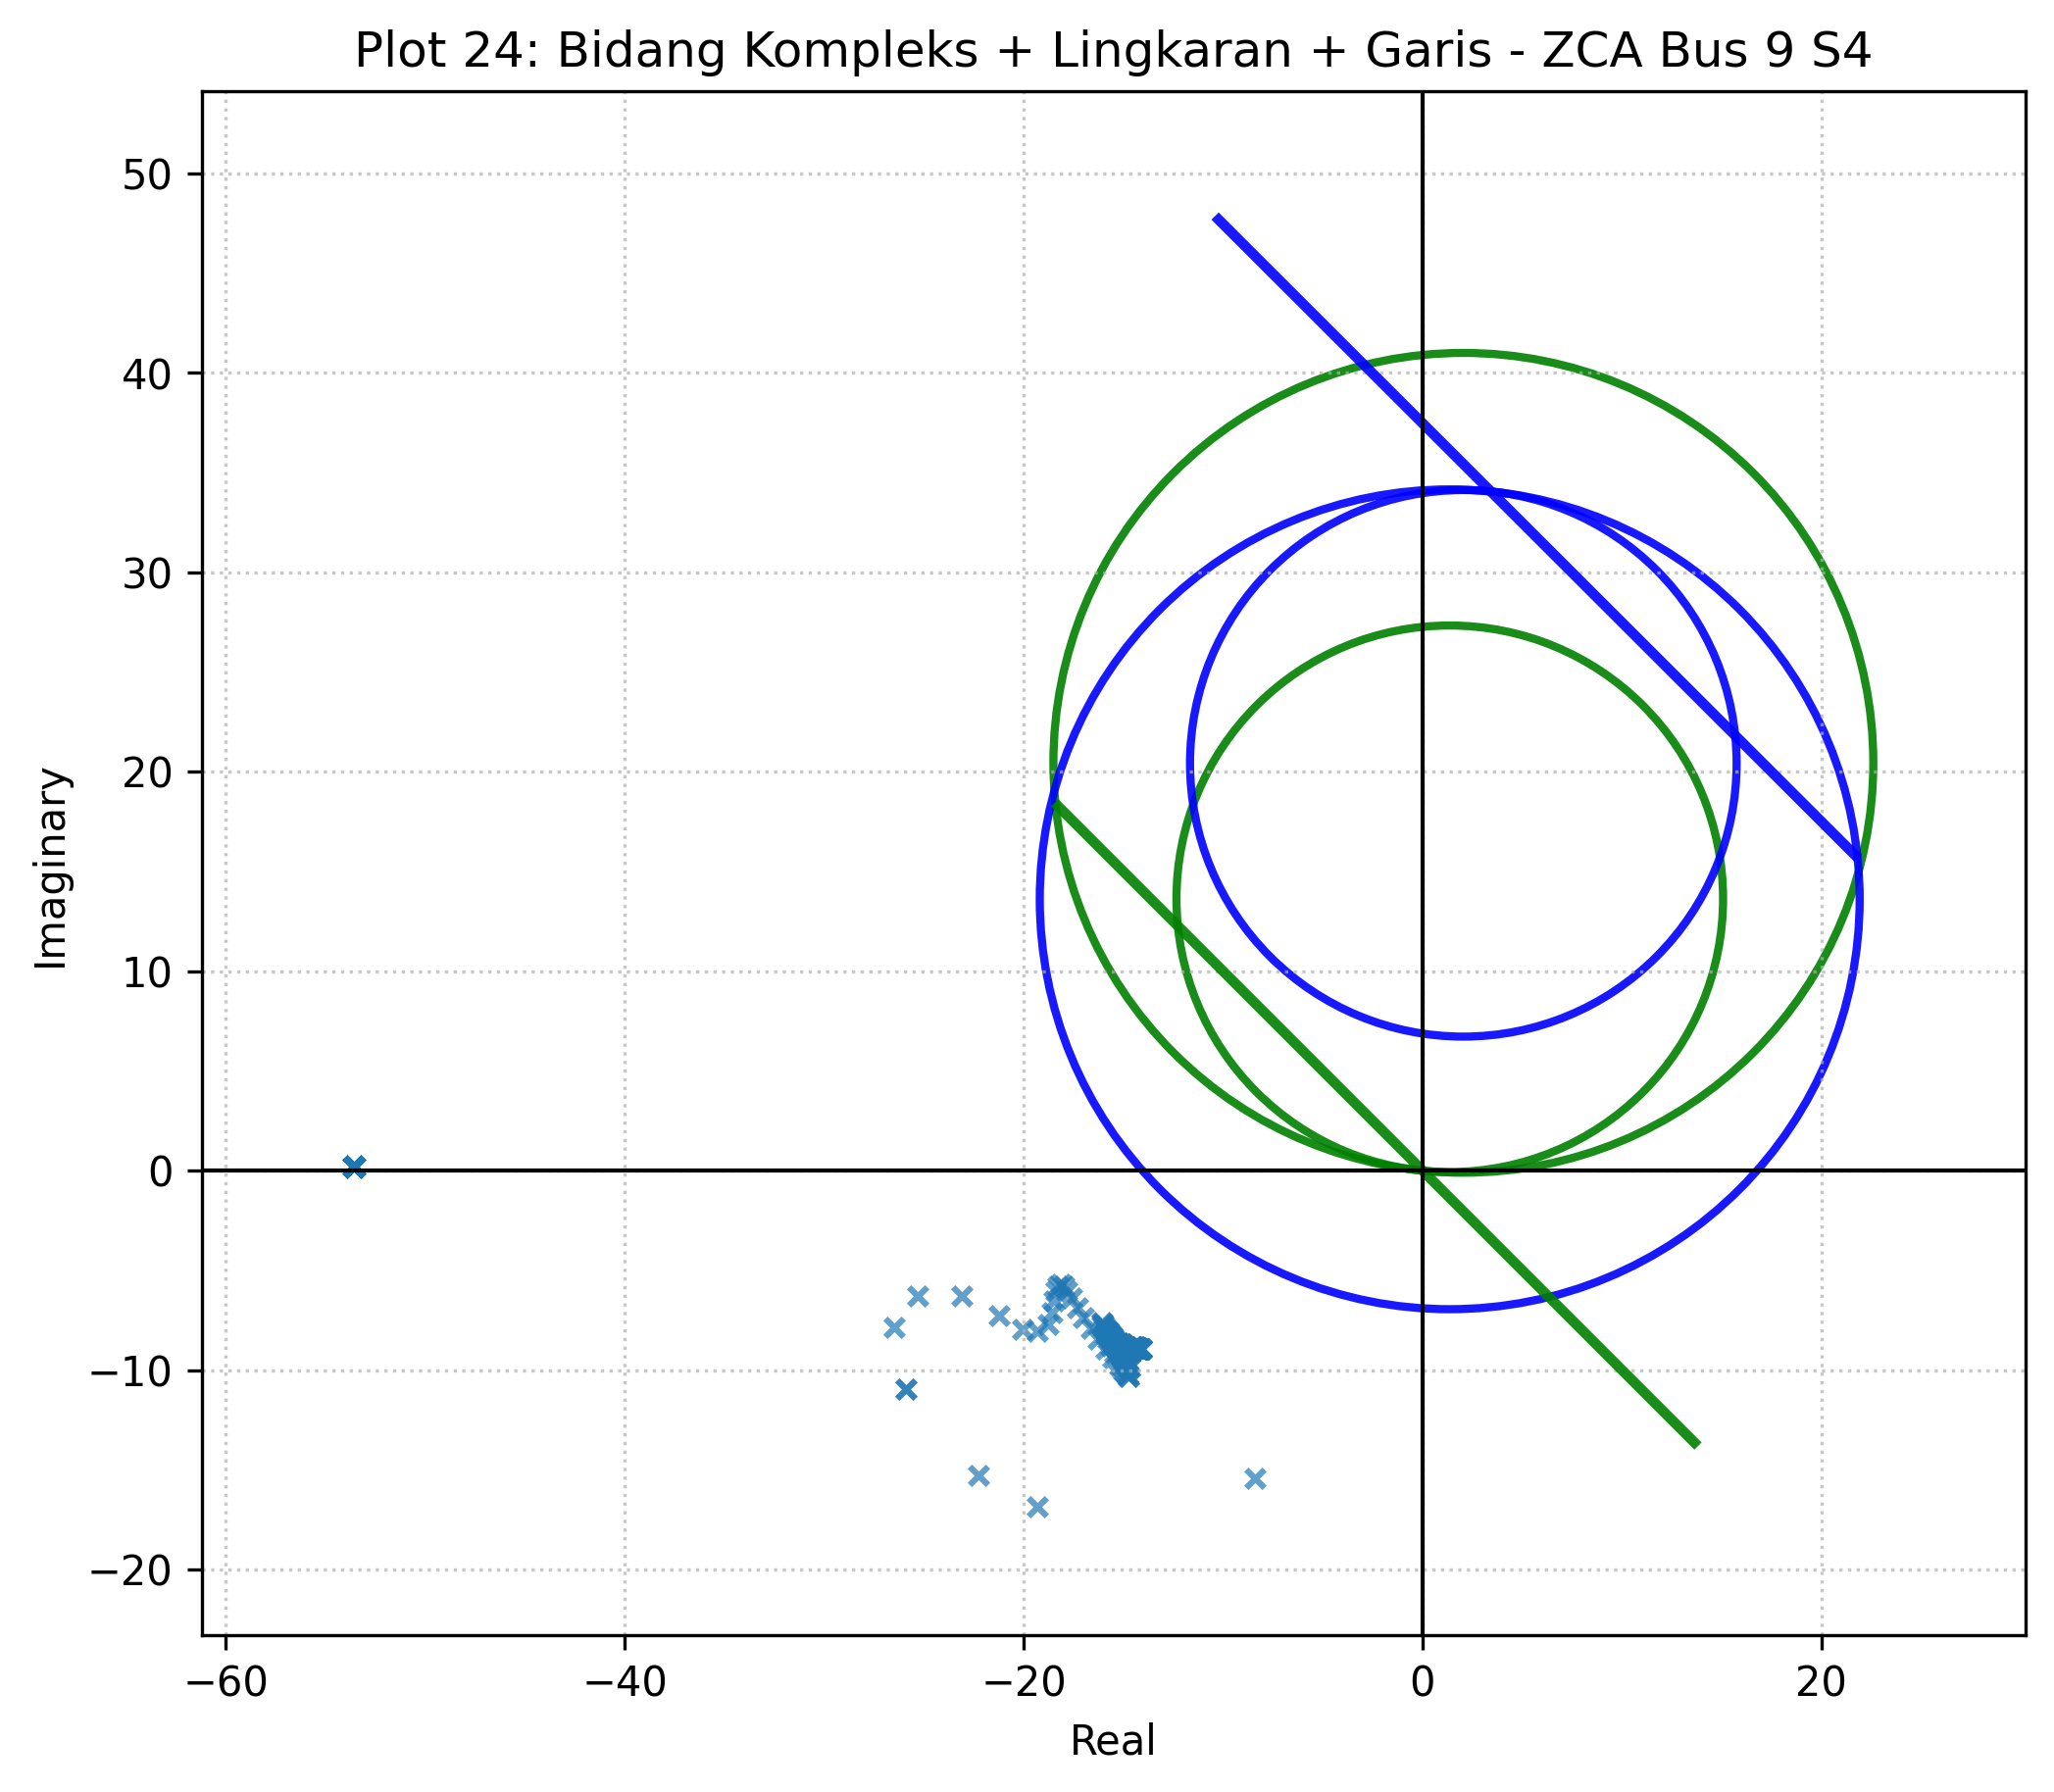
\includegraphics[width=0.8\textwidth]{contents/chapter-4/24_ZCA_Bus_9_S4_dengan_lingkaran_dan_garis.png}
%     \caption{Impedansi Tampak ZCA Bus 9 Skenario 4}
%     \label{fig:24_ZCA_Bus_9_S4_dengan_lingkaran_dan_garis}
% \end{figure}

% Terlihat pada gambar \ref{fig:24_ZCA_Bus_9_S4_dengan_lingkaran_dan_garis} bahwa impedansi tampak pada fasa B dengan fasa C yang dibaca oleh relay 21 sisi bus 9 saat terdapat gangguan bekerja dengan baik sesuai acuan pada \ref{subsec:tanpa_IBR_ex_3p} relay 21 bus 9 tidak mendeteksi adanya gangguan sehingga tidak mengirimkan sinyal trip kepada CB.

%%%%%%%%%%%%%%%%%%%%%%%%%%%%%%%%%SISI PRIMER%%%%%%%%%%%%%%%%%%%%%%%%%%%%%%%%%%

% \begin{figure}[H]
%     \centering
%     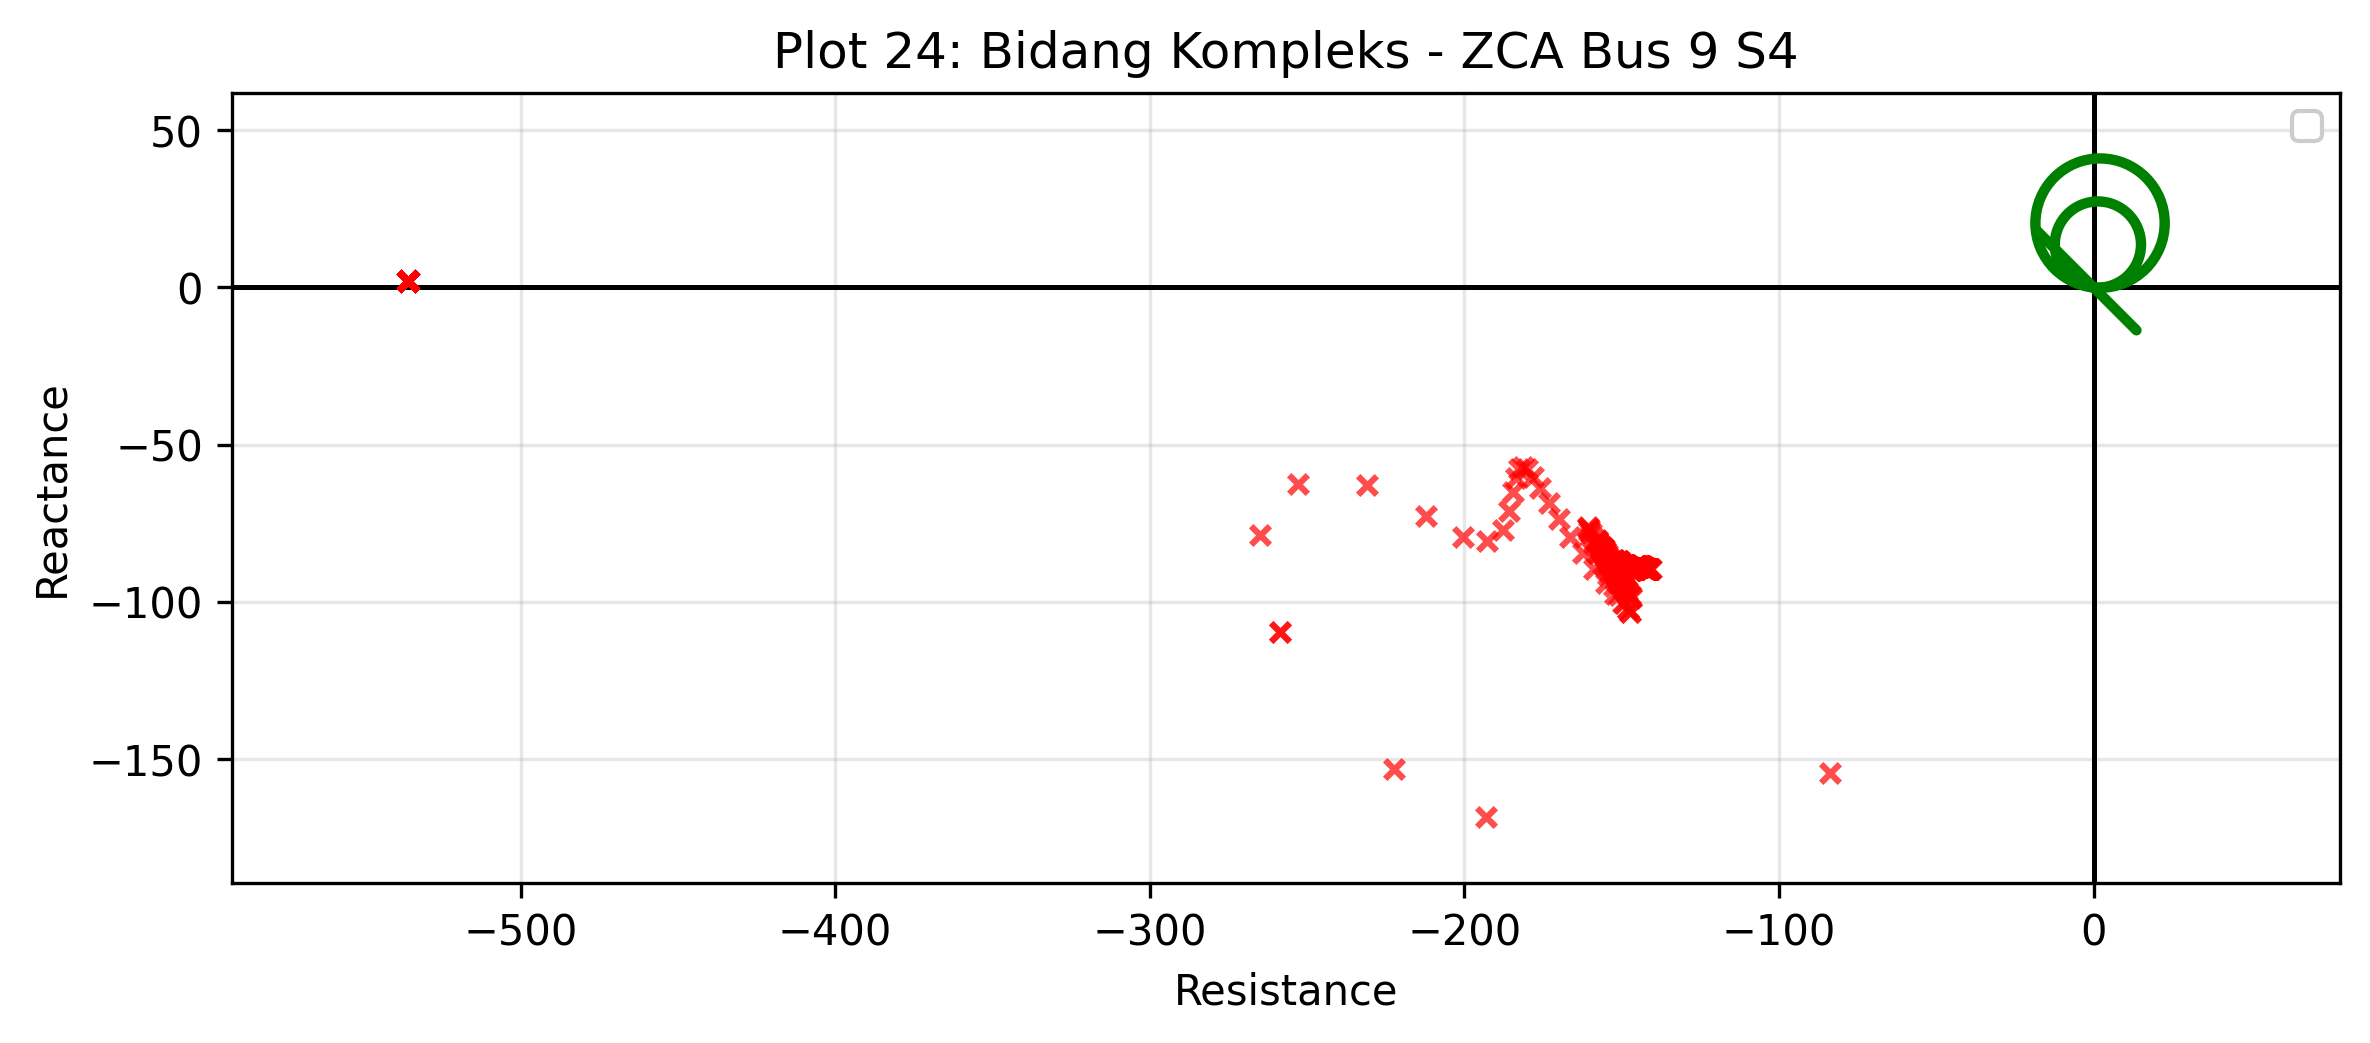
\includegraphics[width=0.8\textwidth]{contents/chapter-4/PRIA_24_ZCA_Bus_9_S4.png}
%     \caption{Impedansi Tampak ZCA Bus 9 Skenario 4}
%     \label{fig:PRIA_24_ZCA_Bus_9_S4}
% \end{figure}

% \begin{figure}[H]
%     \centering
%     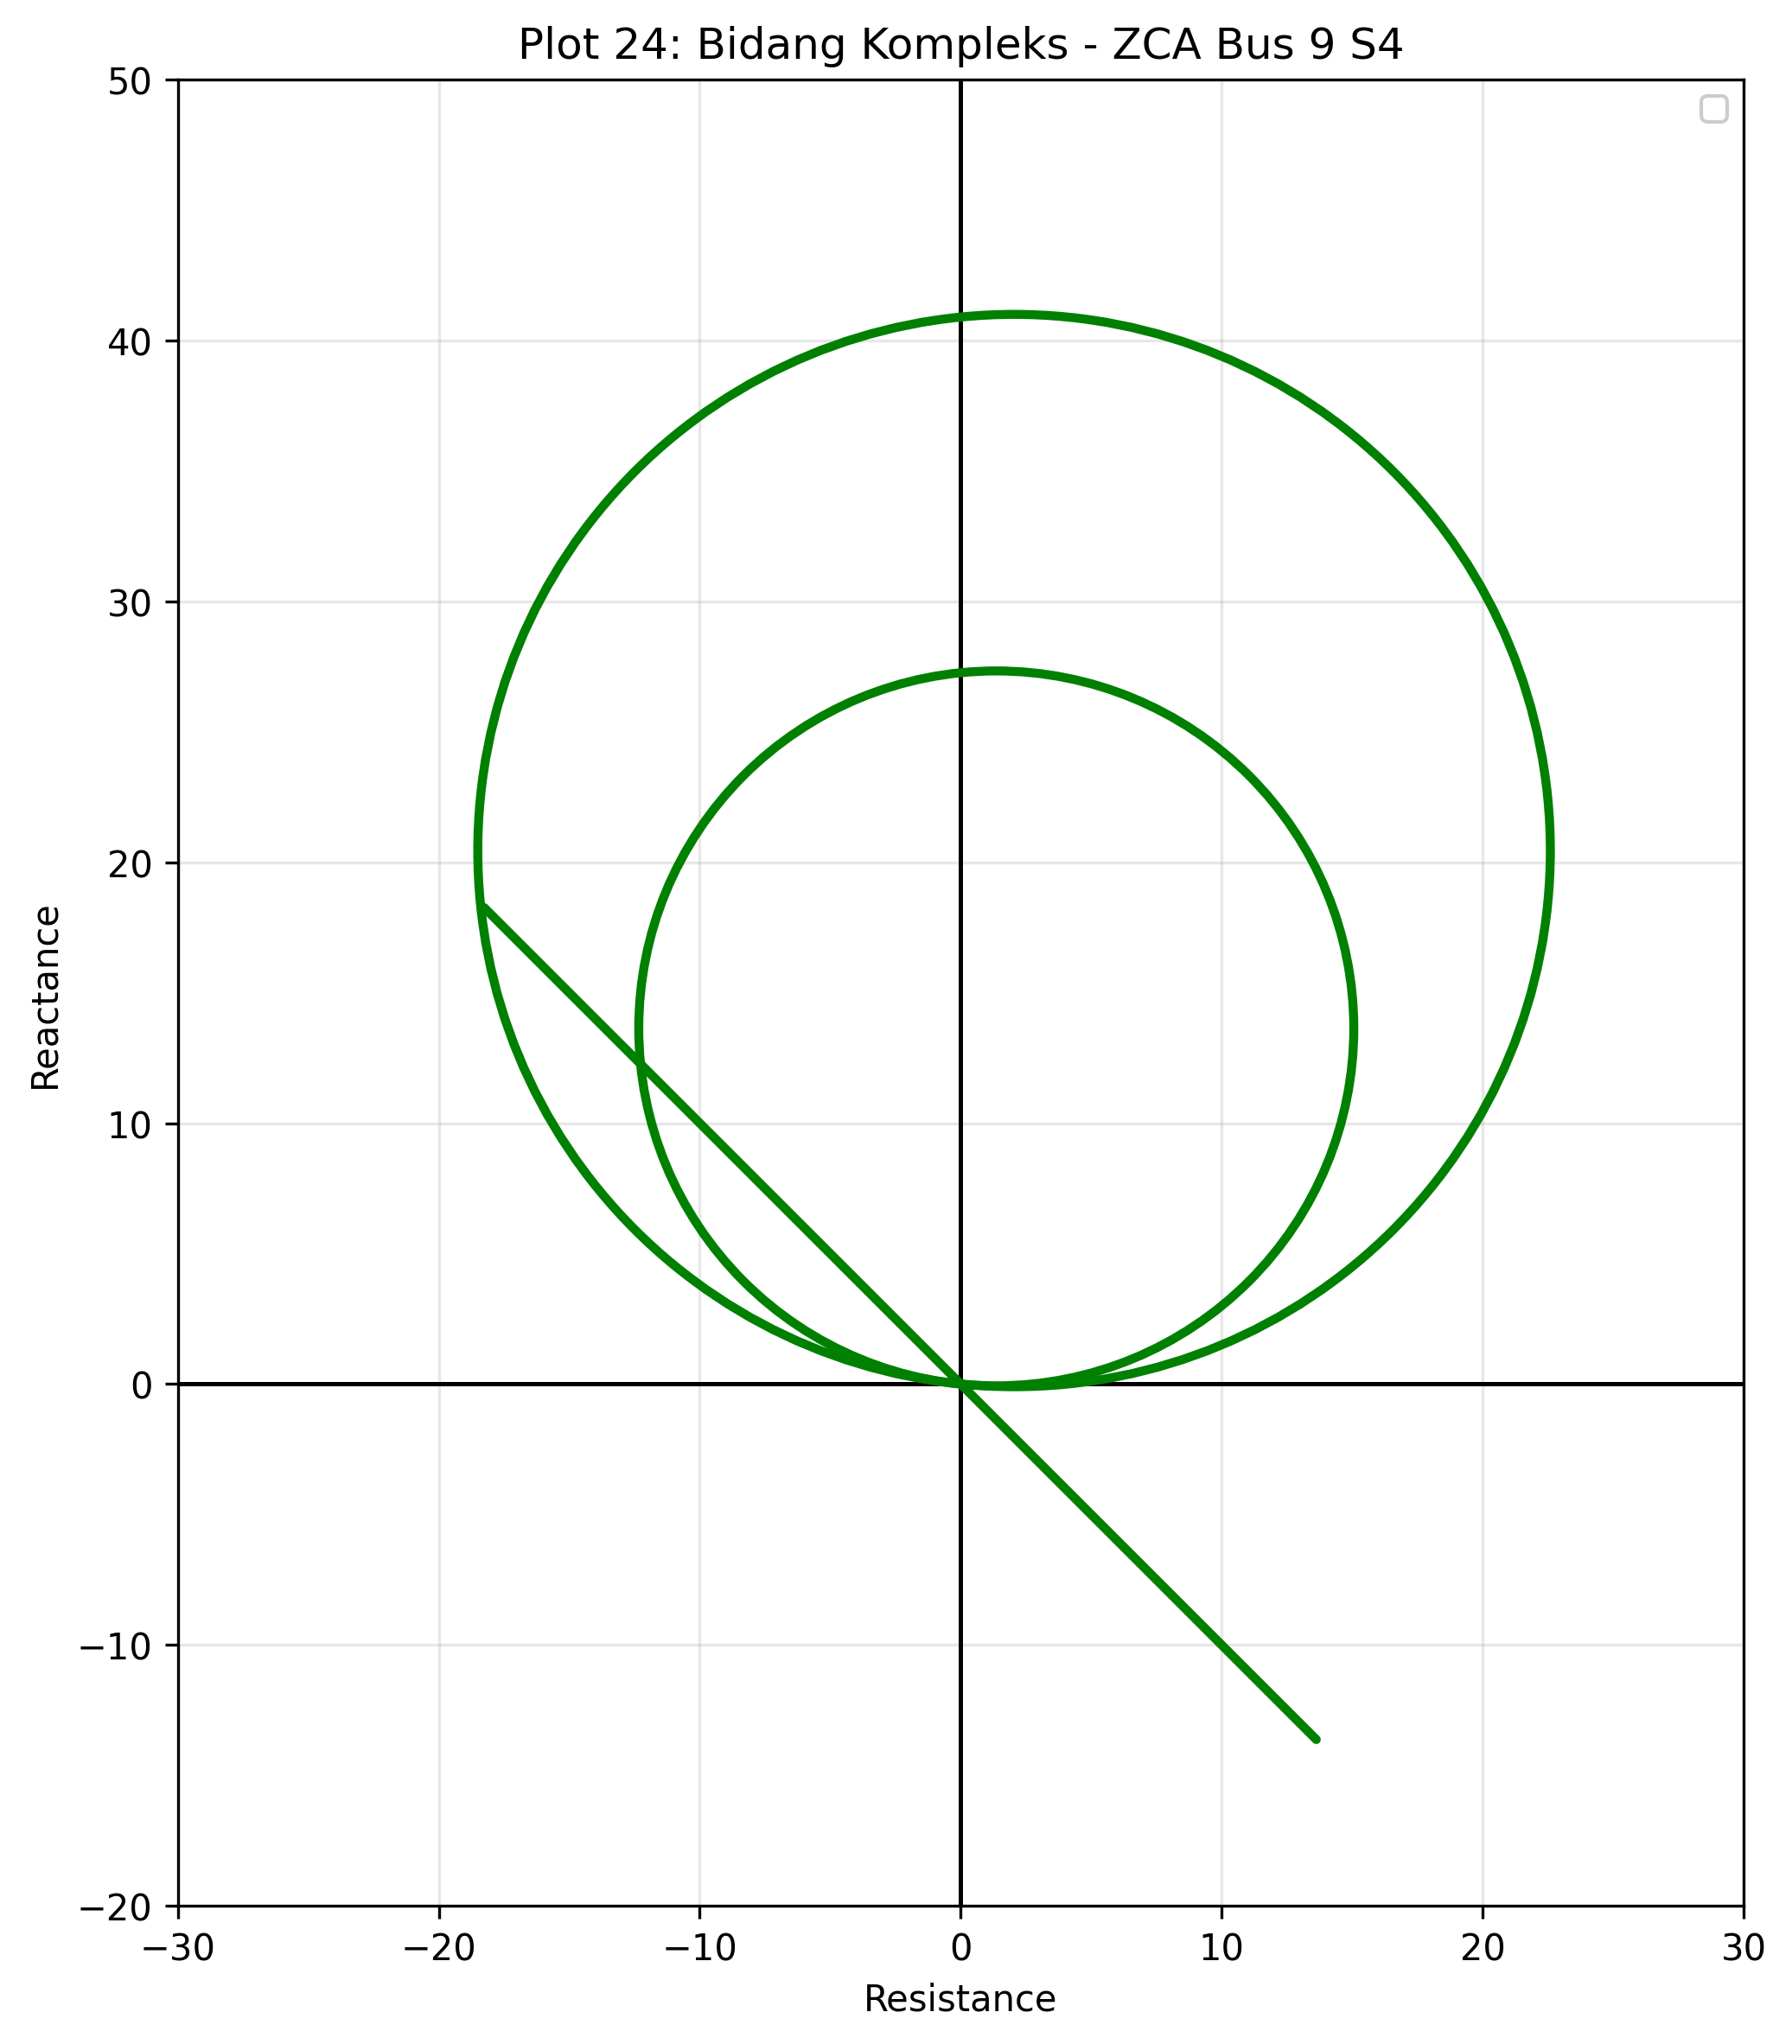
\includegraphics[width=0.8\textwidth]{contents/chapter-4/PRIZI_24_ZCA_Bus_9_S4.png}
%     \caption{Impedansi Tampak ZCA Bus 9 Skenario 4}
%     \label{fig:PRIZI_24_ZCA_Bus_9_S4}
% \end{figure}

\begin{figure}[H]
    \centering

    % Gambar sebelah kiri
    \begin{subfigure}[t]{0.48\textwidth}
        \centering
        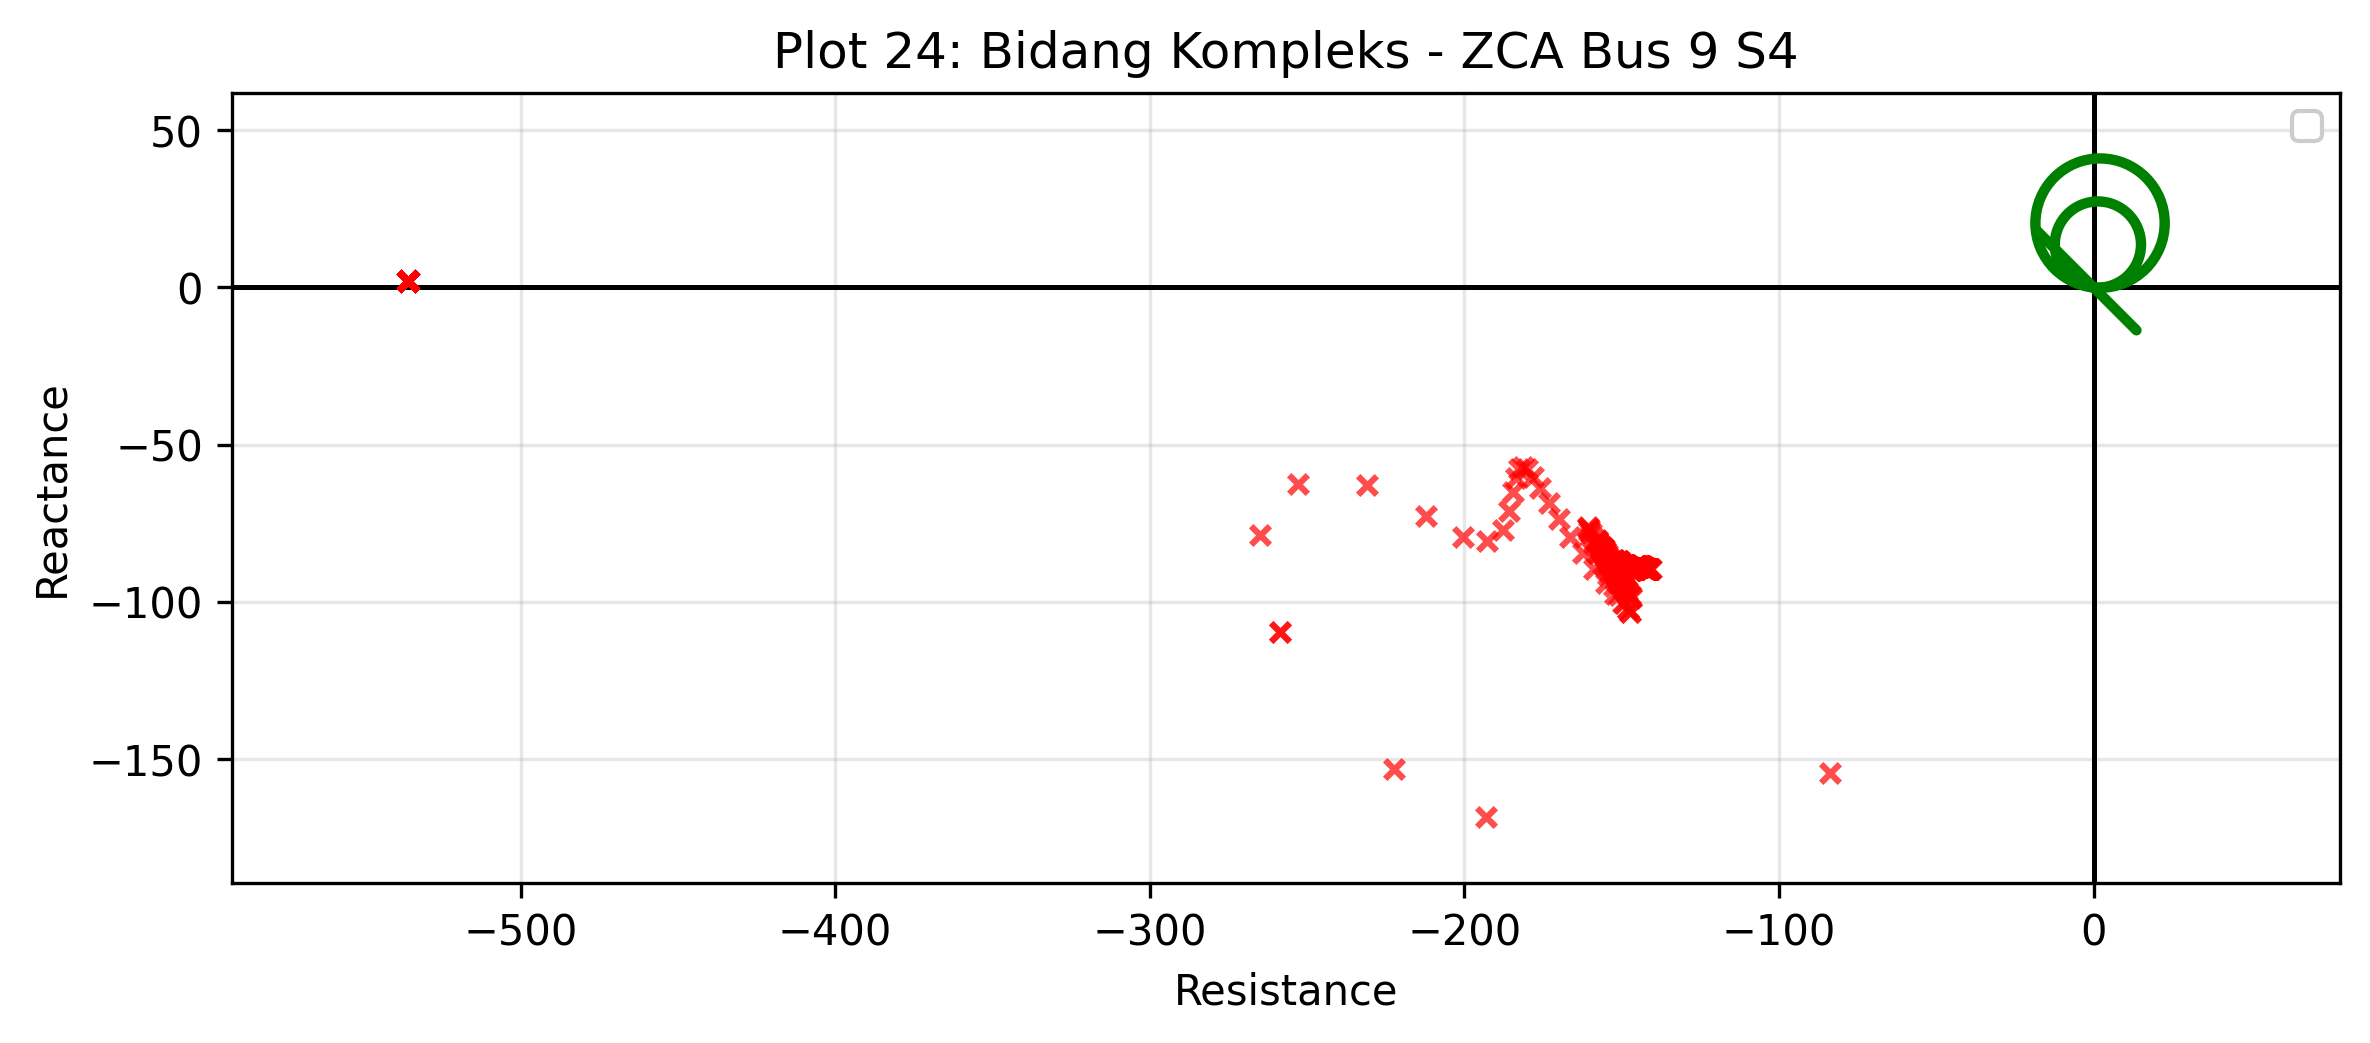
\includegraphics[width=\textwidth]{contents/chapter-4/PRIA_24_ZCA_Bus_9_S4.png}
        \caption{Seluruh Impedansi Tampak}
        \label{fig:PRIA_24_ZCA_Bus_9_S4}
    \end{subfigure}
    \hfill
    % Gambar sebelah kanan
    \begin{subfigure}[t]{0.48\textwidth}
        \centering
        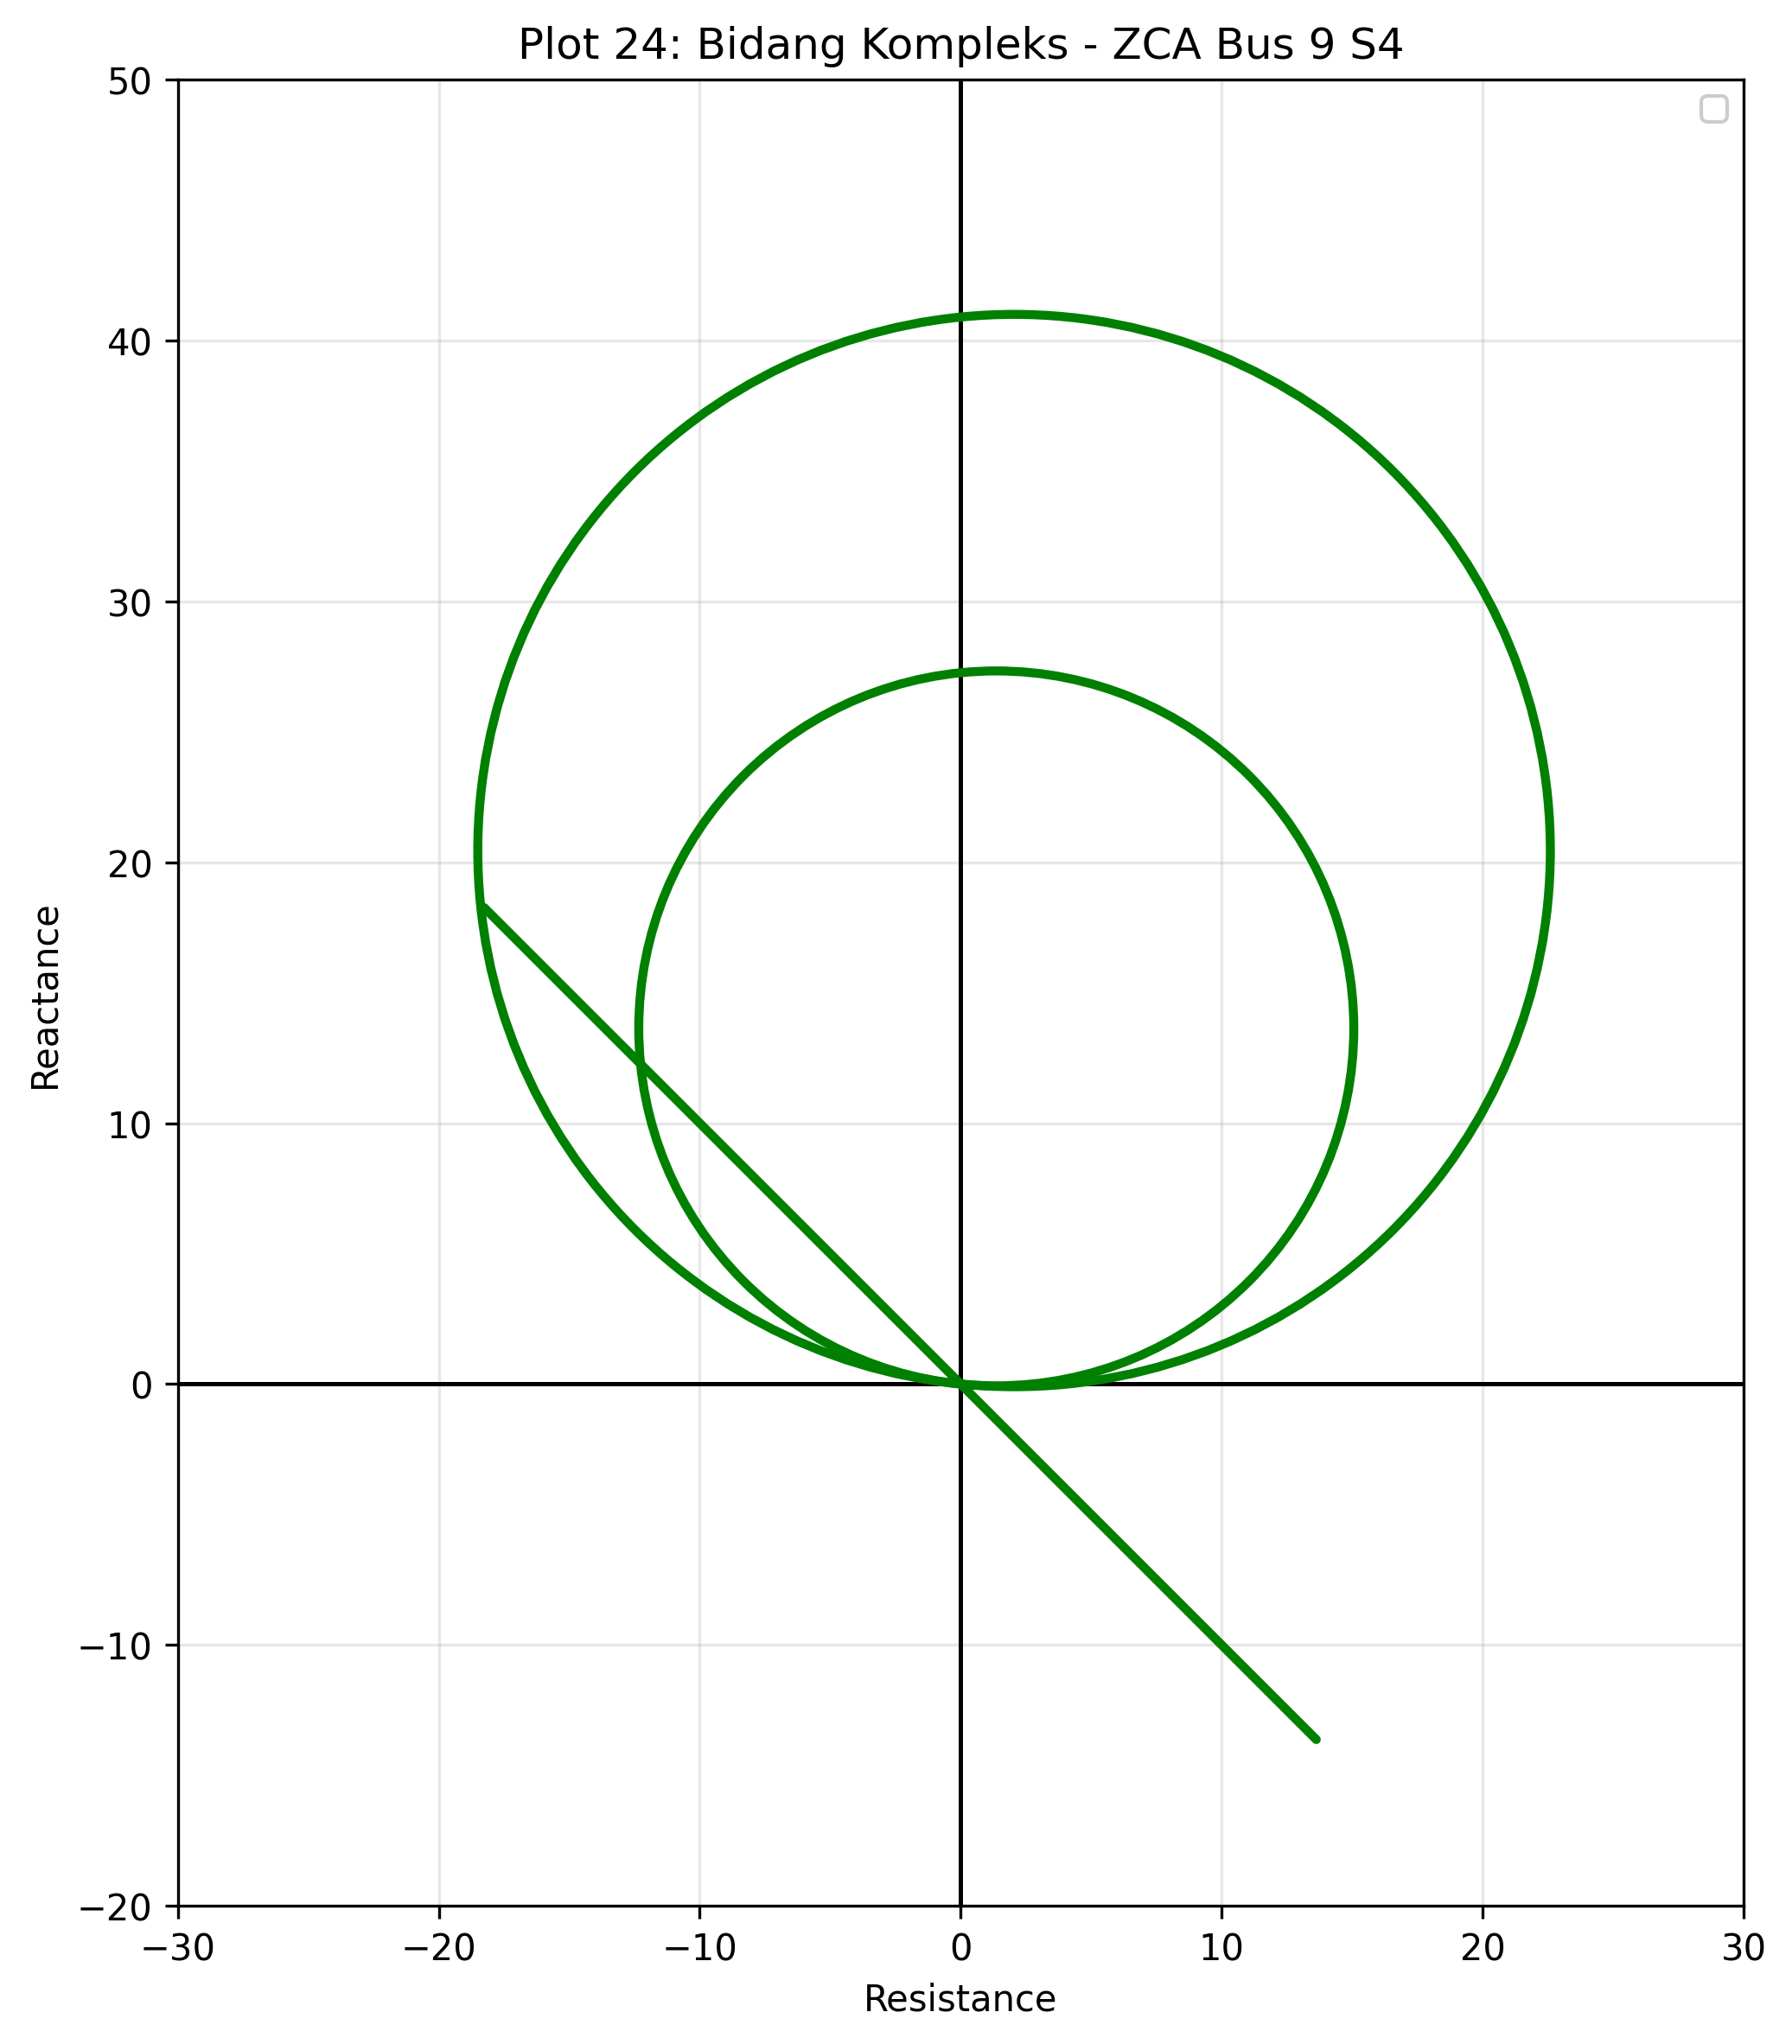
\includegraphics[width=\textwidth]{contents/chapter-4/PRIZI_24_ZCA_Bus_9_S4.png}
        \caption{Zoom In Pada Zona Proteksi}
        \label{fig:PRIZI_24_ZCA_Bus_9_S4}
    \end{subfigure}

    \caption{Impedansi Tampak ZCA Bus 9 Skenario 4}
    \label{fig:Impedansi_Tampak_ZCA_Bus_9_S4}
\end{figure}

Terlihat pada gambar \ref{fig:Impedansi_Tampak_ZCA_Bus_9_S4} bahwa impedansi tampak pada fasa B dengan fasa C yang dibaca oleh relay 21 sisi bus 9 saat terdapat gangguan bekerja dengan baik sesuai acuan pada \ref{subsec:tanpa_IBR_ex_3p} relay 21 bus 9 tidak mendeteksi adanya gangguan sehingga tidak mengirimkan sinyal trip kepada CB.

%%%%%%%%%%%%%%%%%%%%%%%%%%%%%%%%%%%%%%%%%%%%%%%%%%%%%%%%%%%%%%%



% pada gambar \ref{fig:19_ZAB_Bus_8_S4_dengan_lingkaran_dan_garis} hingga \ref{fig:21_ZCA_Bus_8_S4_dengan_lingkaran_dan_garis} menunjukkan impedansi tampak yang dibaca oleh relay 21 dari sisi bus 8 dimana menunjukkan bahwa relay mengalami misoperation overreach ke zona 1 serta mengalami dropout pada zona 2. Kemudian pada gambar \ref{fig:22_ZAB_Bus_9_S4_dengan_lingkaran_dan_garis} hingga \ref{fig:24_ZCA_Bus_9_S4_dengan_lingkaran_dan_garis} menunjukkan impedansi tampak yang dibaca oleh relay 21 pada sisi bus 9 dimana menunjukkan relay berjalan normal sebagimana mestinya.



\subsection{Skenario 5 : Wind Turbine Type 3 External SLG Fault}

Skenario ini membahas gangguan eksternal satu fasa ke tanah pada sistem dengan \textit{wind turbine type 3}. Jenis gangguan ini penting karena melibatkan komponen urutan nol dan kompensasi urutan nol pada elemen jarak fasa-tanah, sehingga perubahan arus yang terbaca dapat memengaruhi pembentukan impedansi tampak relay 21.

Hasil dekomposisi komponen urutan arus pada Gambar \ref{fig:decomposition_sequence_current_s5} digunakan untuk menghubungkan karakter arus gangguan dengan pembacaan relay pada TL89. Setelah itu, analisis diarahkan pada elemen ZAG dari sisi Bus 8 dan Bus 9 untuk melihat apakah relay tetap sesuai dengan acuan gangguan eksternal atau mengalami perubahan respons akibat rendahnya arus yang terbaca.

% \begin{figure}[H]
%     \centering
%     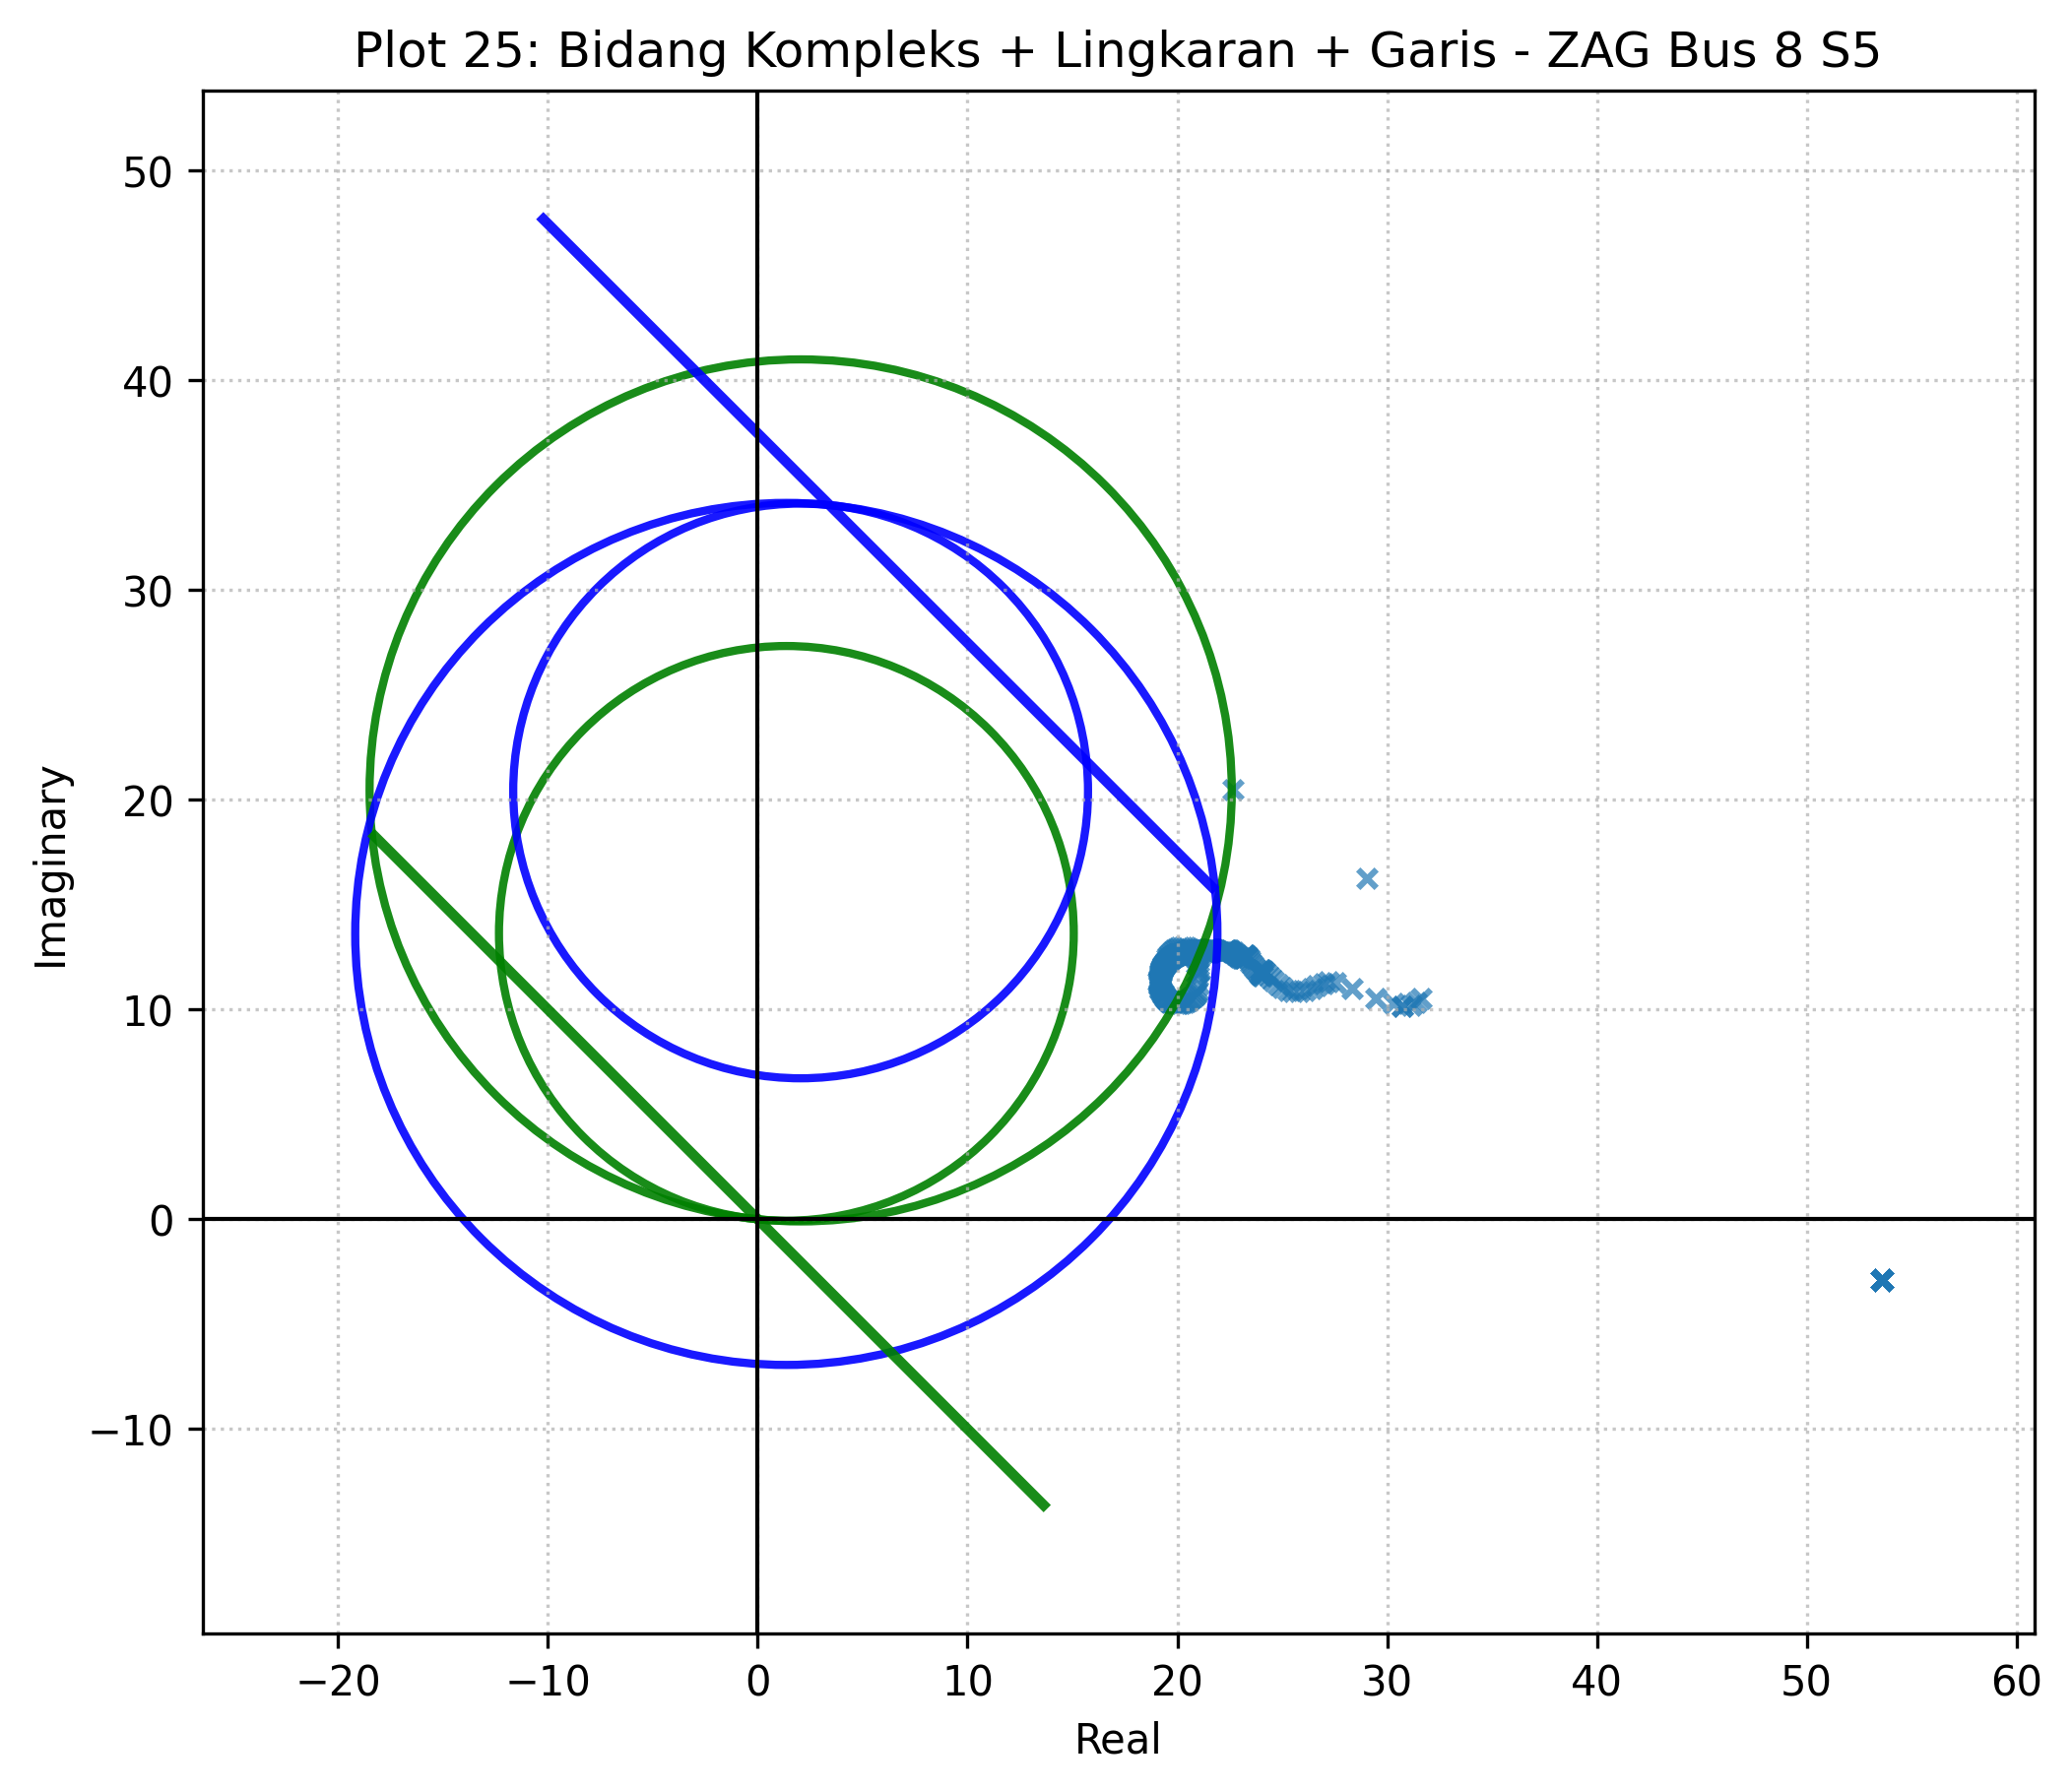
\includegraphics[width=0.8\textwidth]{contents/chapter-4/25_ZAG_Bus_8_S5_dengan_lingkaran_dan_garis.png}
%     \caption{Impedansi Tampak ZAG Bus 8 Skenario 5}
%     \label{fig:25_ZAG_Bus_8_S5_dengan_lingkaran_dan_garis}
% \end{figure}

% Terlihat pada gambar \ref{fig:25_ZAG_Bus_8_S5_dengan_lingkaran_dan_garis} bahwa impedansi tampak pada fasa A dengan ground yang dibaca oleh relay 21 sisi bus 8 saat terdapat gangguan SLG bekerja dengan dengan acuan pada \ref{subsec:tanpa_IBR_ex_slg} relay 21 bus 8 mendeteksi adanya gangguan pada zona 2 dan memberikan sinyal trip kepada CB.


%%%%%%%%%%%%%%%%%%%%%%%%%%%%%%%%%SISI PRIMER%%%%%%%%%%%%%%%%%%%%%%%%%%%%%%%%%%

\begin{figure}[H]
    \centering
    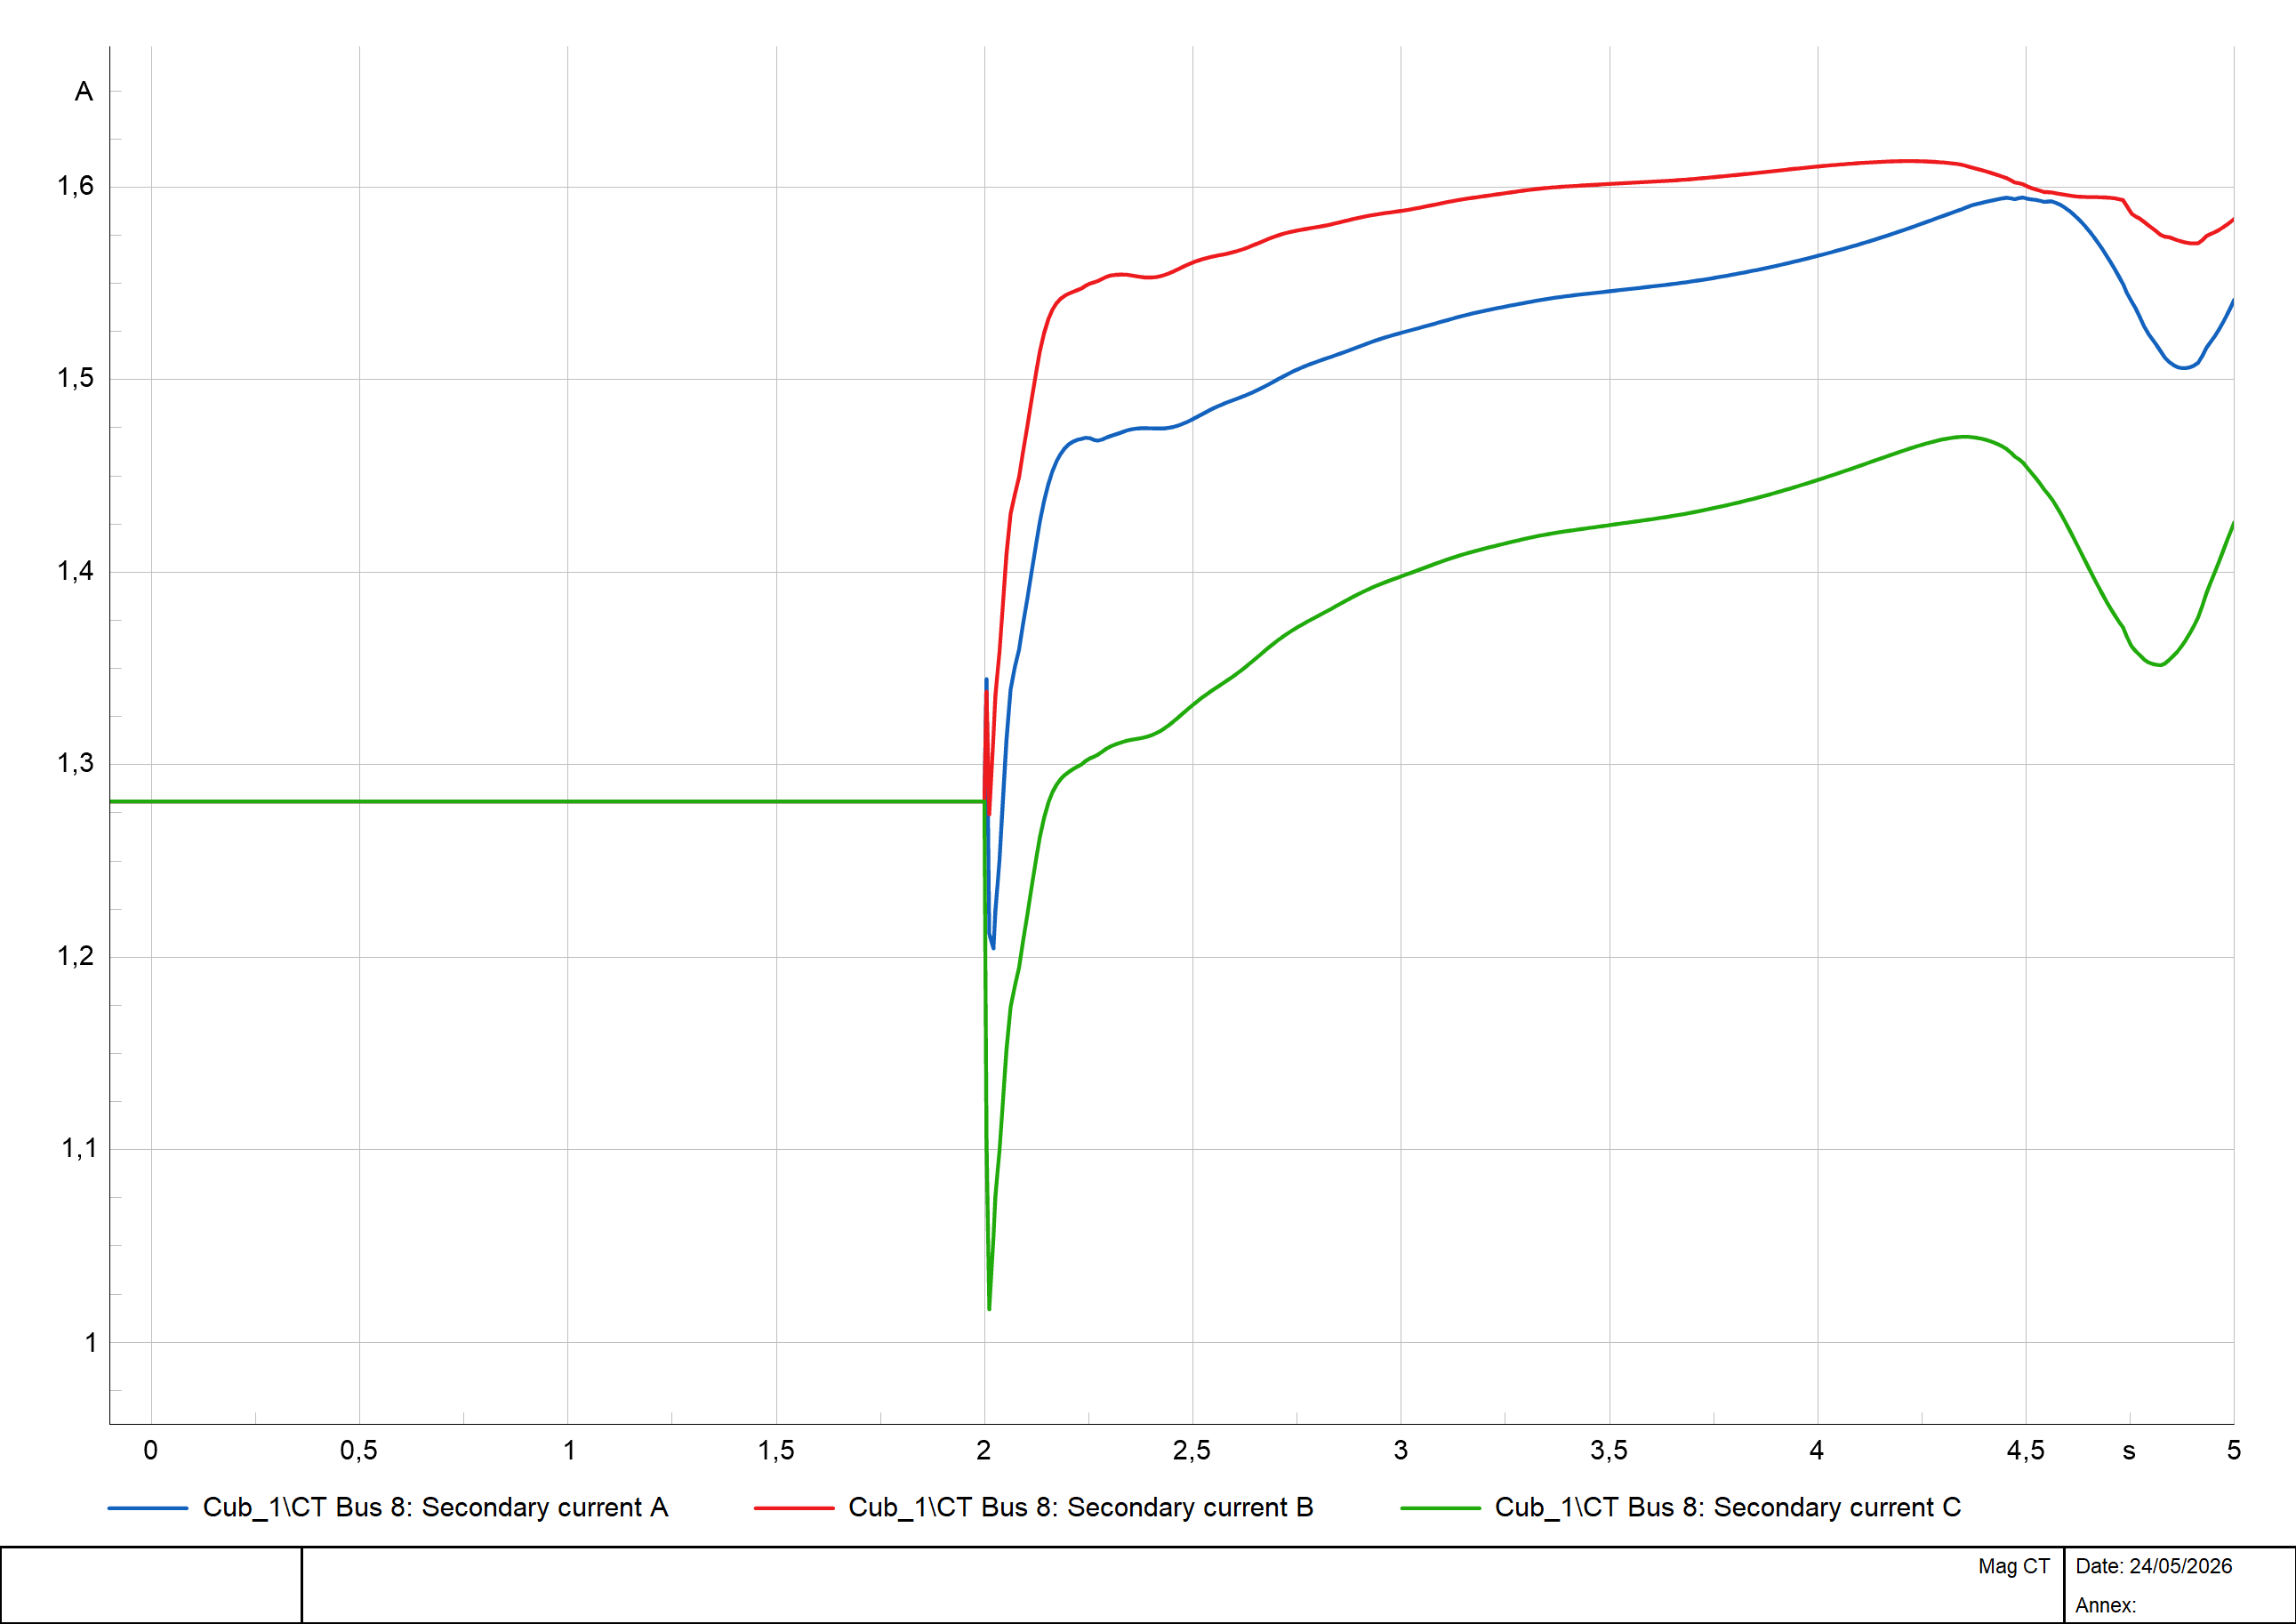
\includegraphics[width=0.8\textwidth]{contents/chapter-4/Bus_8_Ex_SLG_S5.png}
    \caption{Arus Sekunder CT Bus 8 Skenario 5}
    \label{fig:Bus_8_Ex_SLG_S5}
\end{figure}

Gambar \ref{fig:Bus_8_Ex_SLG_S5} menunjukkan arus sekunder CT pada Bus 8 untuk skenario 5 saat terjadi gangguan eksternal SLG. Sebelum gangguan, arus pada ketiga fasa berada pada nilai 1,281 A sekunder. Setelah gangguan terjadi, arus fasa A meningkat menjadi 1,595 A sekunder atau 1,25 p.u., arus fasa B meningkat menjadi 1,613 A sekunder atau 1,26 p.u., dan arus fasa C meningkat menjadi 1,47 A sekunder atau 1,15 p.u. Kenaikan arus tersebut menunjukkan adanya perubahan arus saat gangguan, tetapi nilainya masih belum memenuhi arus minimum yang diperlukan untuk membuat relay 21 sisi Bus 8 aktif.

\begin{figure}[H]
    \centering

    % Gambar sebelah kiri
    \begin{subfigure}[t]{0.48\textwidth}
        \centering
        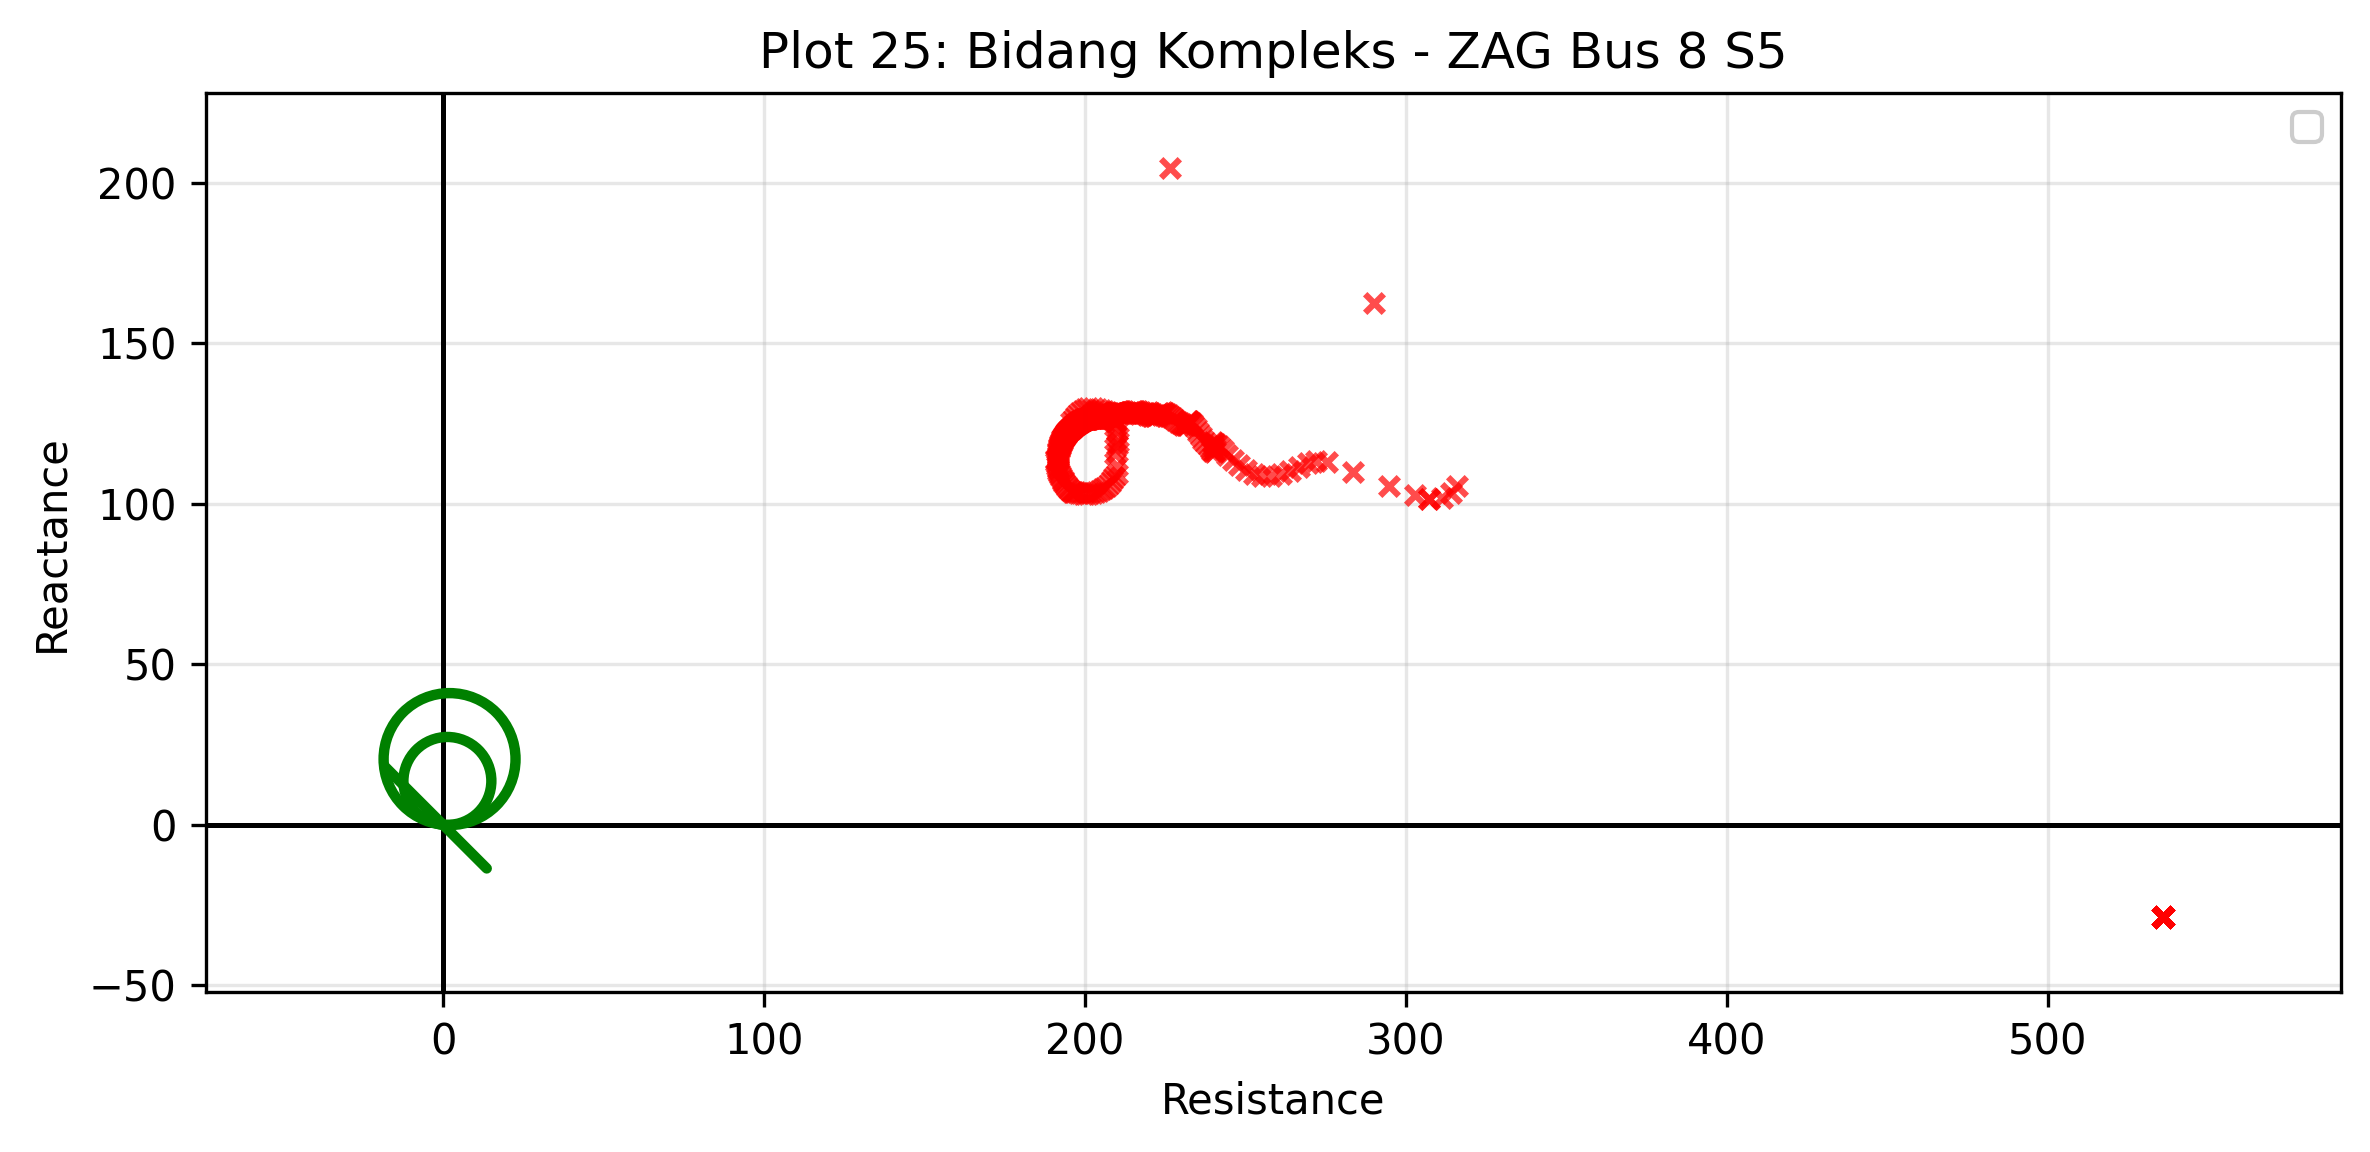
\includegraphics[width=\textwidth]{contents/chapter-4/PRIA_25_ZAG_Bus_8_S5.png}
        \caption{Seluruh Impedansi Tampak}
        \label{fig:PRIA_25_ZAG_Bus_8_S5}
    \end{subfigure}
    \hfill
    % Gambar sebelah kanan
    \begin{subfigure}[t]{0.48\textwidth}
        \centering
        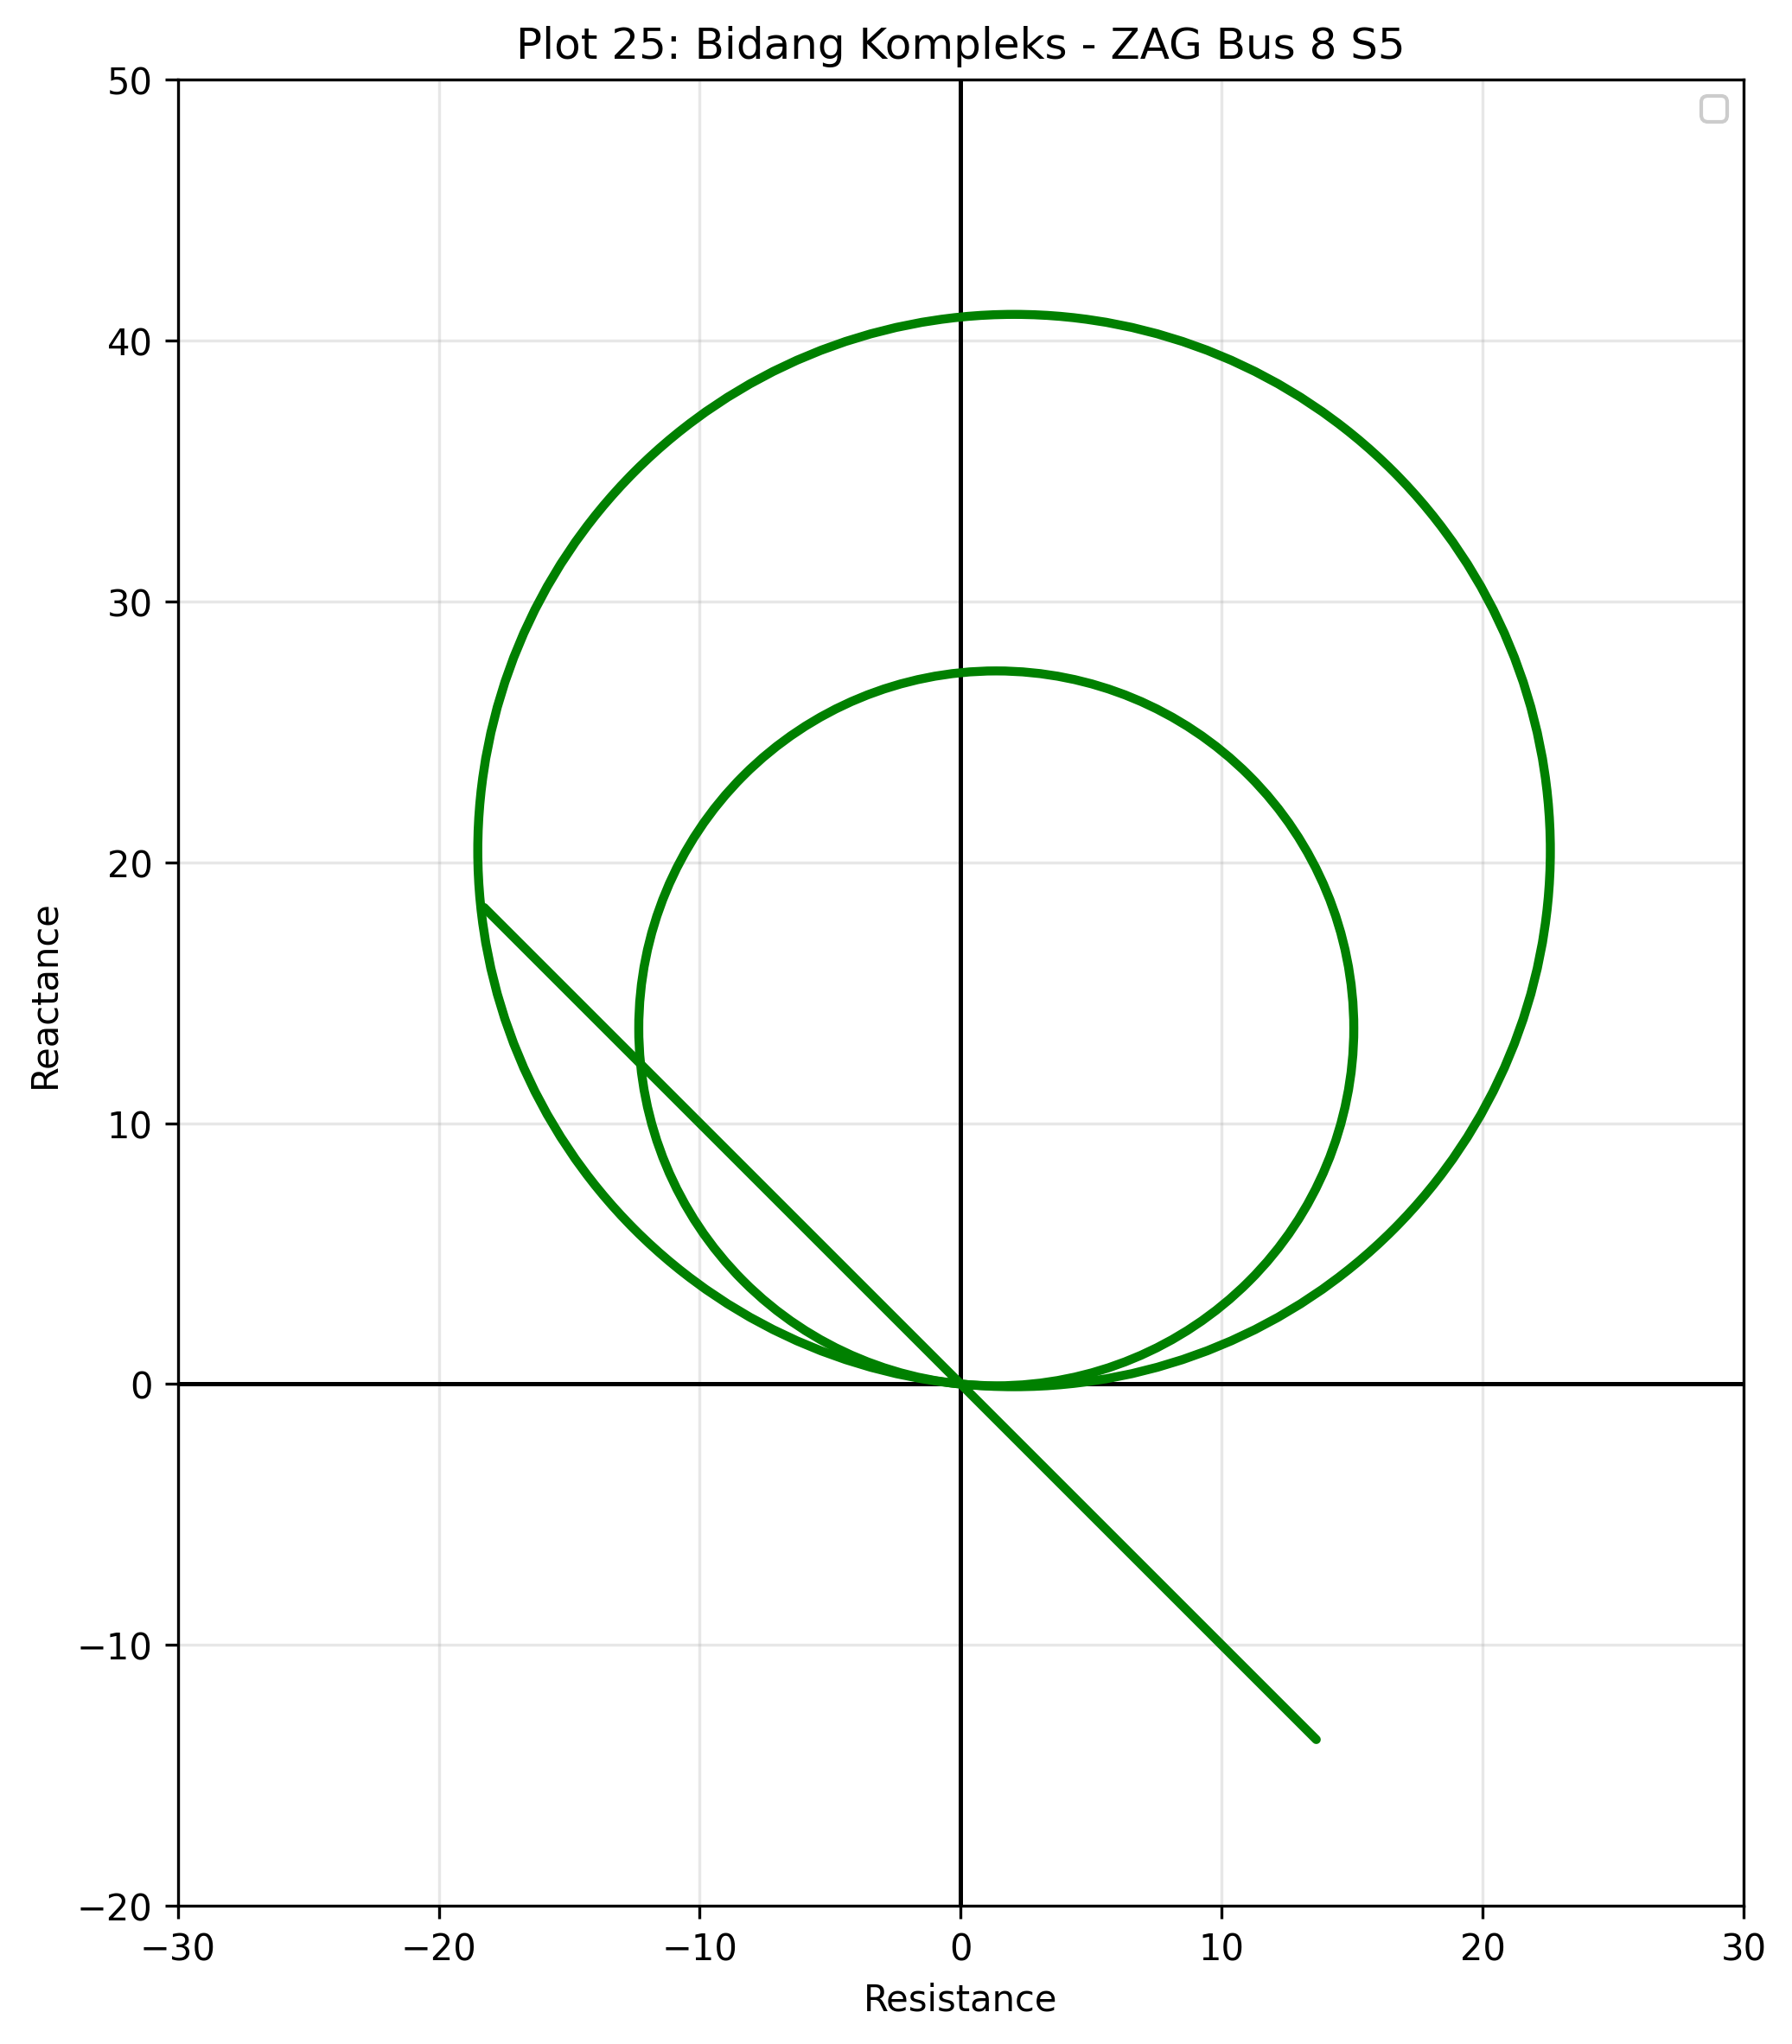
\includegraphics[width=\textwidth]{contents/chapter-4/PRIZI_25_ZAG_Bus_8_S5.png}
        \caption{Zoom In Pada Zona Proteksi}
        \label{fig:PRIZI_25_ZAG_Bus_8_S5}
    \end{subfigure}

    \caption{Impedansi Tampak ZAG Bus 8 Skenario 5}
    \label{fig:Impedansi_Tampak_ZAG_Bus_8_S5}
\end{figure}

Gambar \ref{fig:Impedansi_Tampak_ZAG_Bus_8_S5} menunjukkan bahwa impedansi tampak loop fasa A dengan ground yang dibaca oleh relay 21 sisi Bus 8 tidak masuk ke dalam zona proteksi. Kondisi ini sejalan dengan pembacaan arus sekunder CT pada Gambar \ref{fig:Bus_8_Ex_SLG_S5}, karena arus gangguan yang terbaca masih cukup kecil dan belum memenuhi syarat \textit{starting} untuk membuat relay aktif. Dengan mengacu pada kondisi dasar gangguan eksternal SLG pada Subbab \ref{subsec:tanpa_IBR_ex_slg}, respons relay 21 sisi Bus 8 pada skenario 5 dikategorikan mengalami \textit{misoperation}.

%%%%%%%%%%%%%%%%%%%%%%%%%%%%%%%%%%%%%%%%%%%%%%%%%%%%%%%%%%%%%%%

% \begin{figure}[H]
%     \centering
%     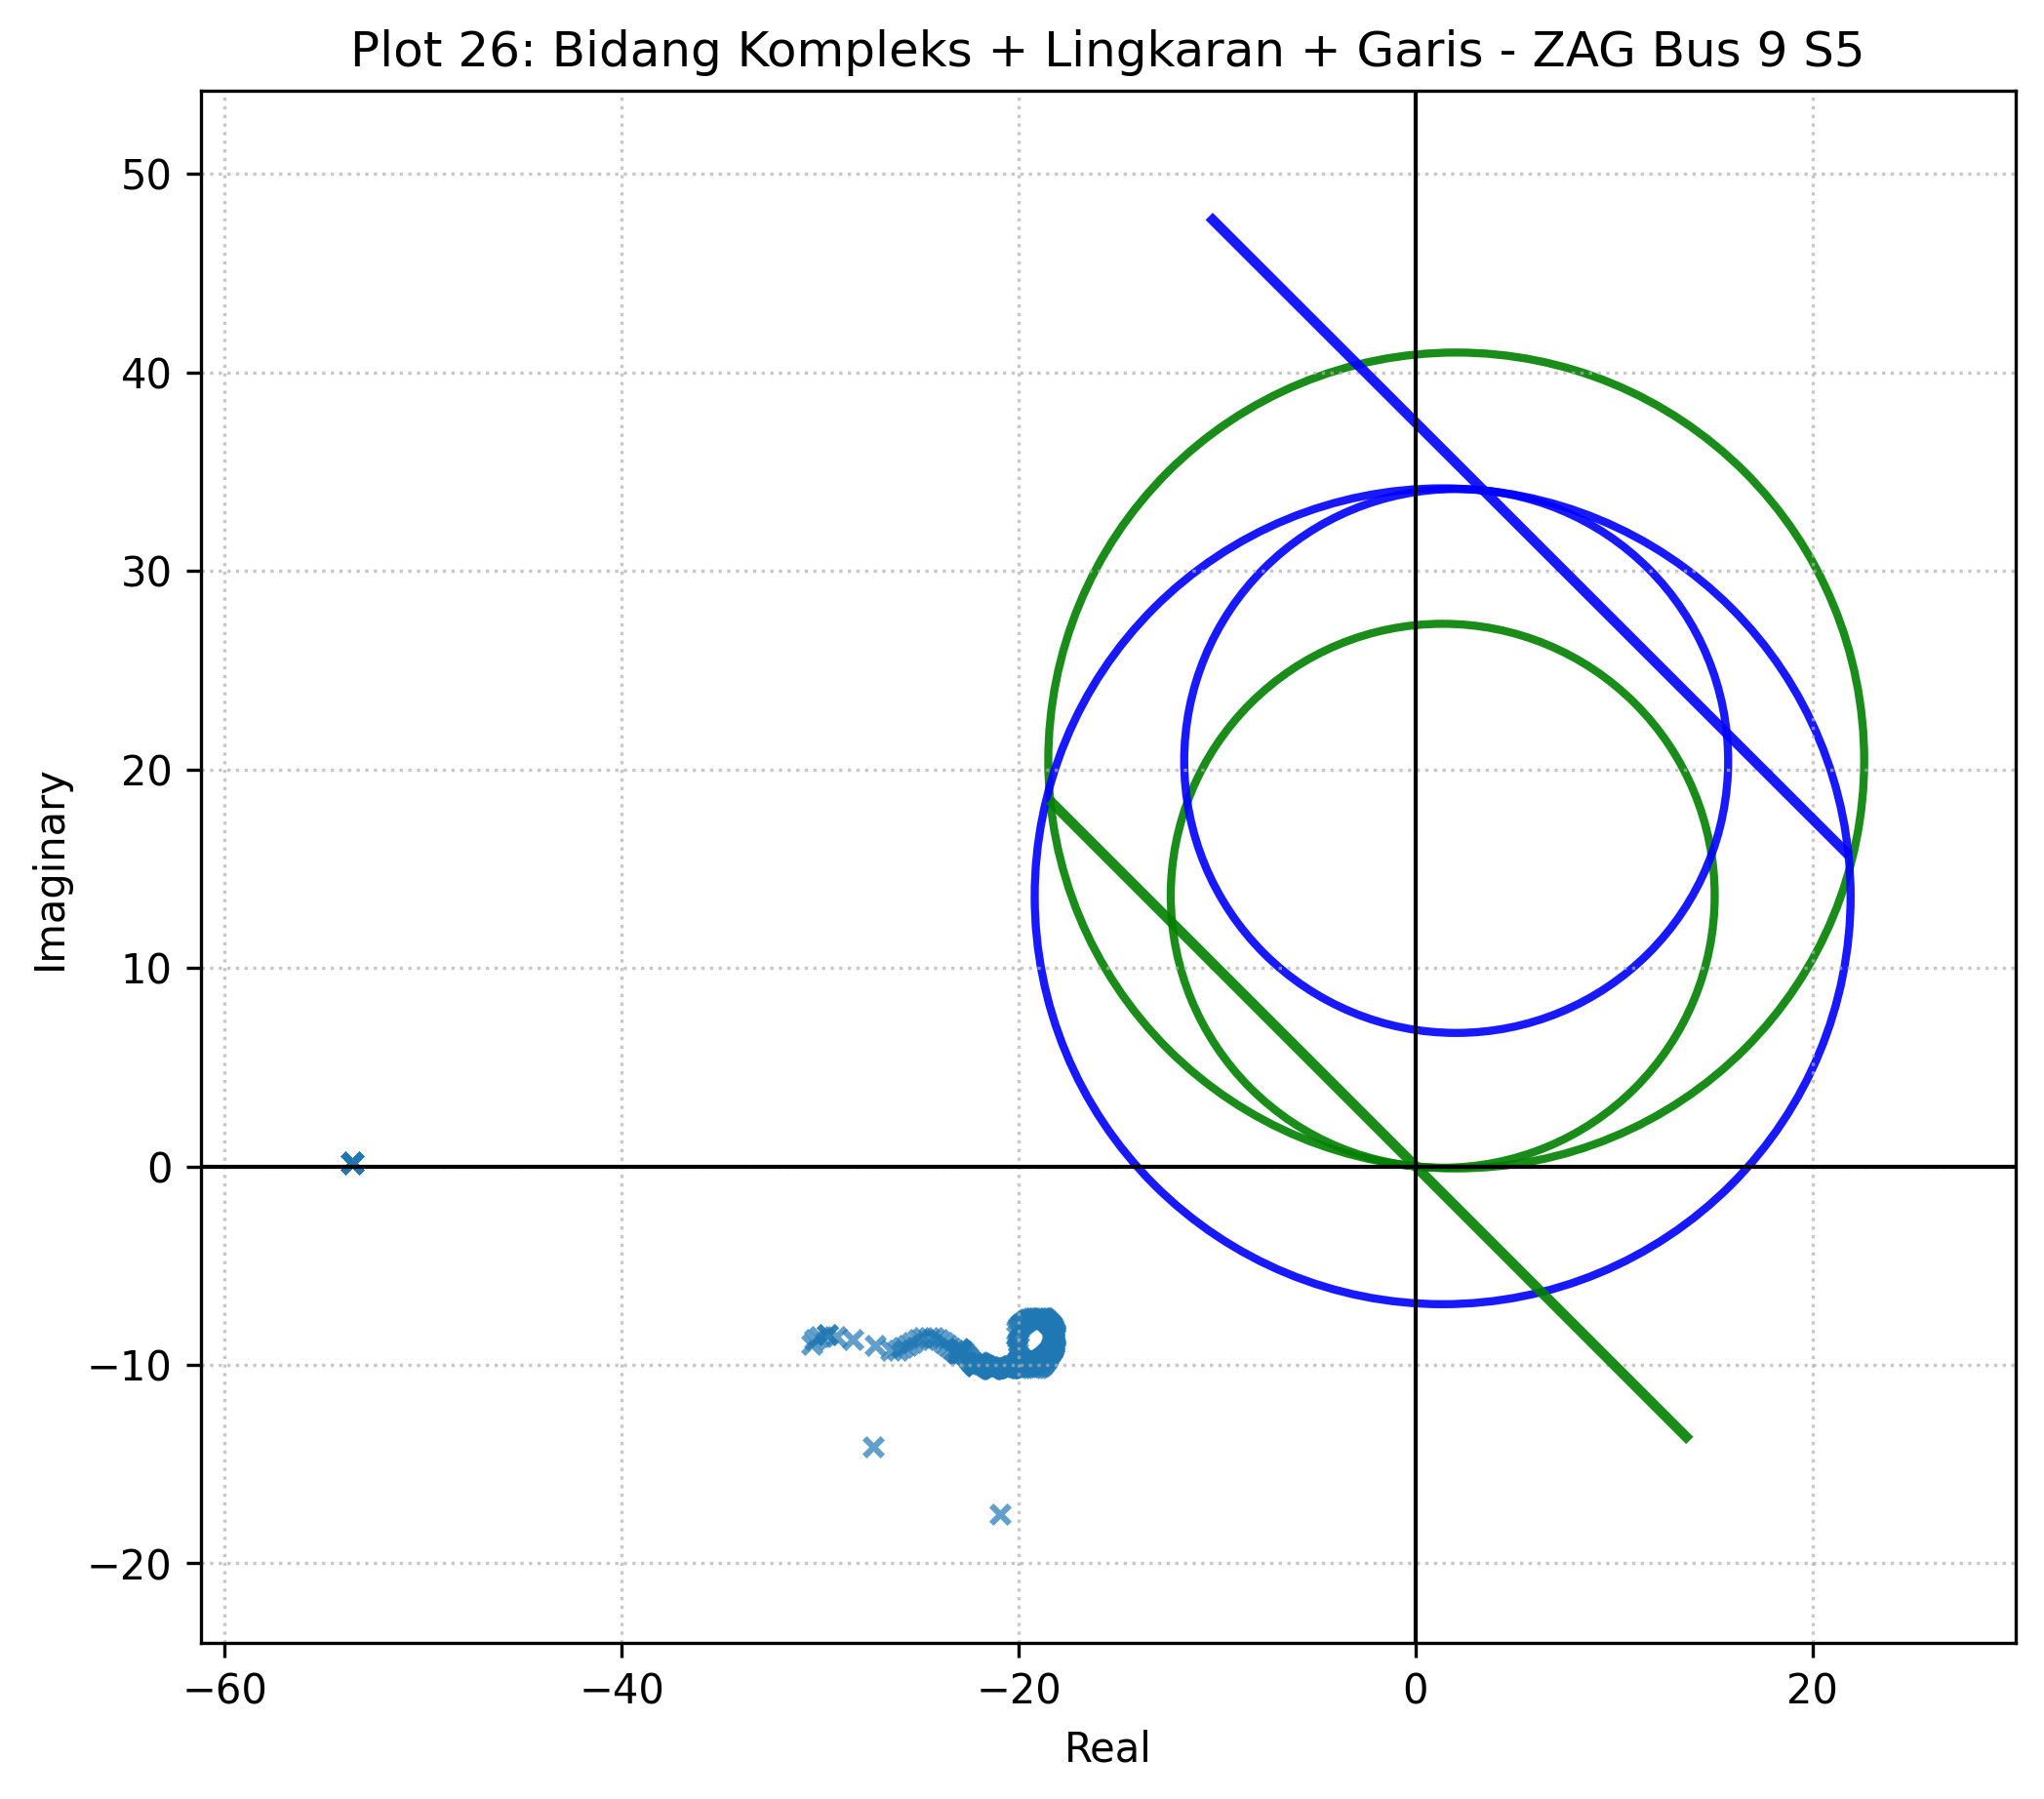
\includegraphics[width=0.8\textwidth]{contents/chapter-4/26_ZAG_Bus_9_S5_dengan_lingkaran_dan_garis.png}
%     \caption{Impedansi Tampak ZAG Bus 9 Skenario 5}
%     \label{fig:26_ZAG_Bus_9_S5_dengan_lingkaran_dan_garis}
% \end{figure}

% Terlihat pada gambar \ref{fig:26_ZAG_Bus_9_S5_dengan_lingkaran_dan_garis} bahwa impedansi tampak pada fasa A dengan ground yang dibaca oleh relay 21 sisi bus 9 saat terdapat gangguan bekerja dengan baik sesuai acuan pada \ref{subsec:tanpa_IBR_ex_slg} relay 21 bus 9 tidak mendeteksi adanya gangguan sehingga tidak mengirimkan sinyal trip kepada CB.

%%%%%%%%%%%%%%%%%%%%%%%%%%%%%%%%%SISI PRIMER%%%%%%%%%%%%%%%%%%%%%%%%%%%%%%%%%%

% \begin{figure}[H]
%     \centering
%     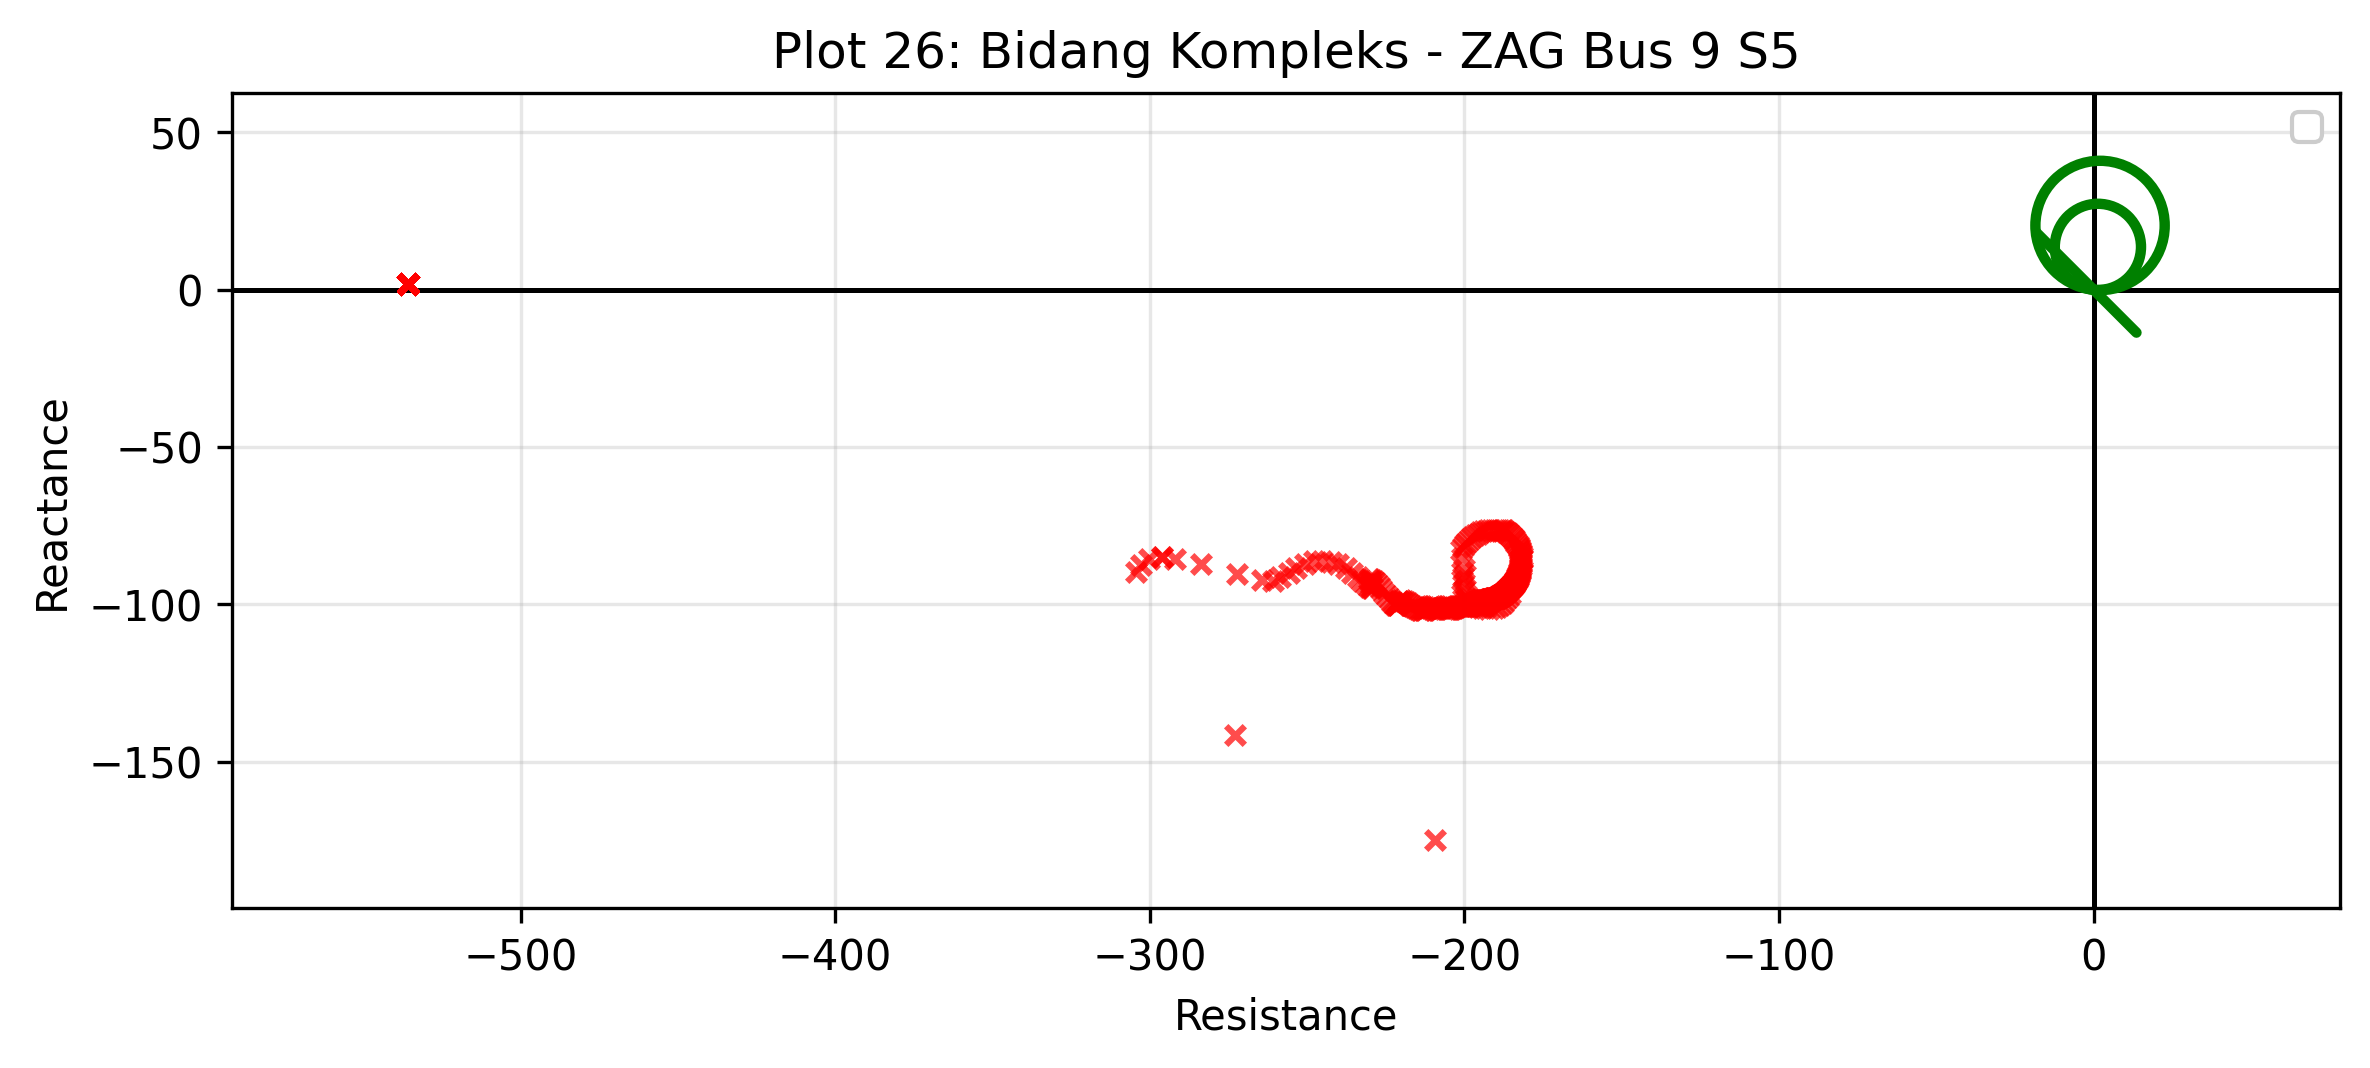
\includegraphics[width=0.8\textwidth]{contents/chapter-4/PRIA_26_ZAG_Bus_9_S5.png}
%     \caption{Impedansi Tampak ZAG Bus 9 Skenario 5}
%     \label{fig:PRIA_26_ZAG_Bus_9_S5}
% \end{figure}

% \begin{figure}[H]
%     \centering
%     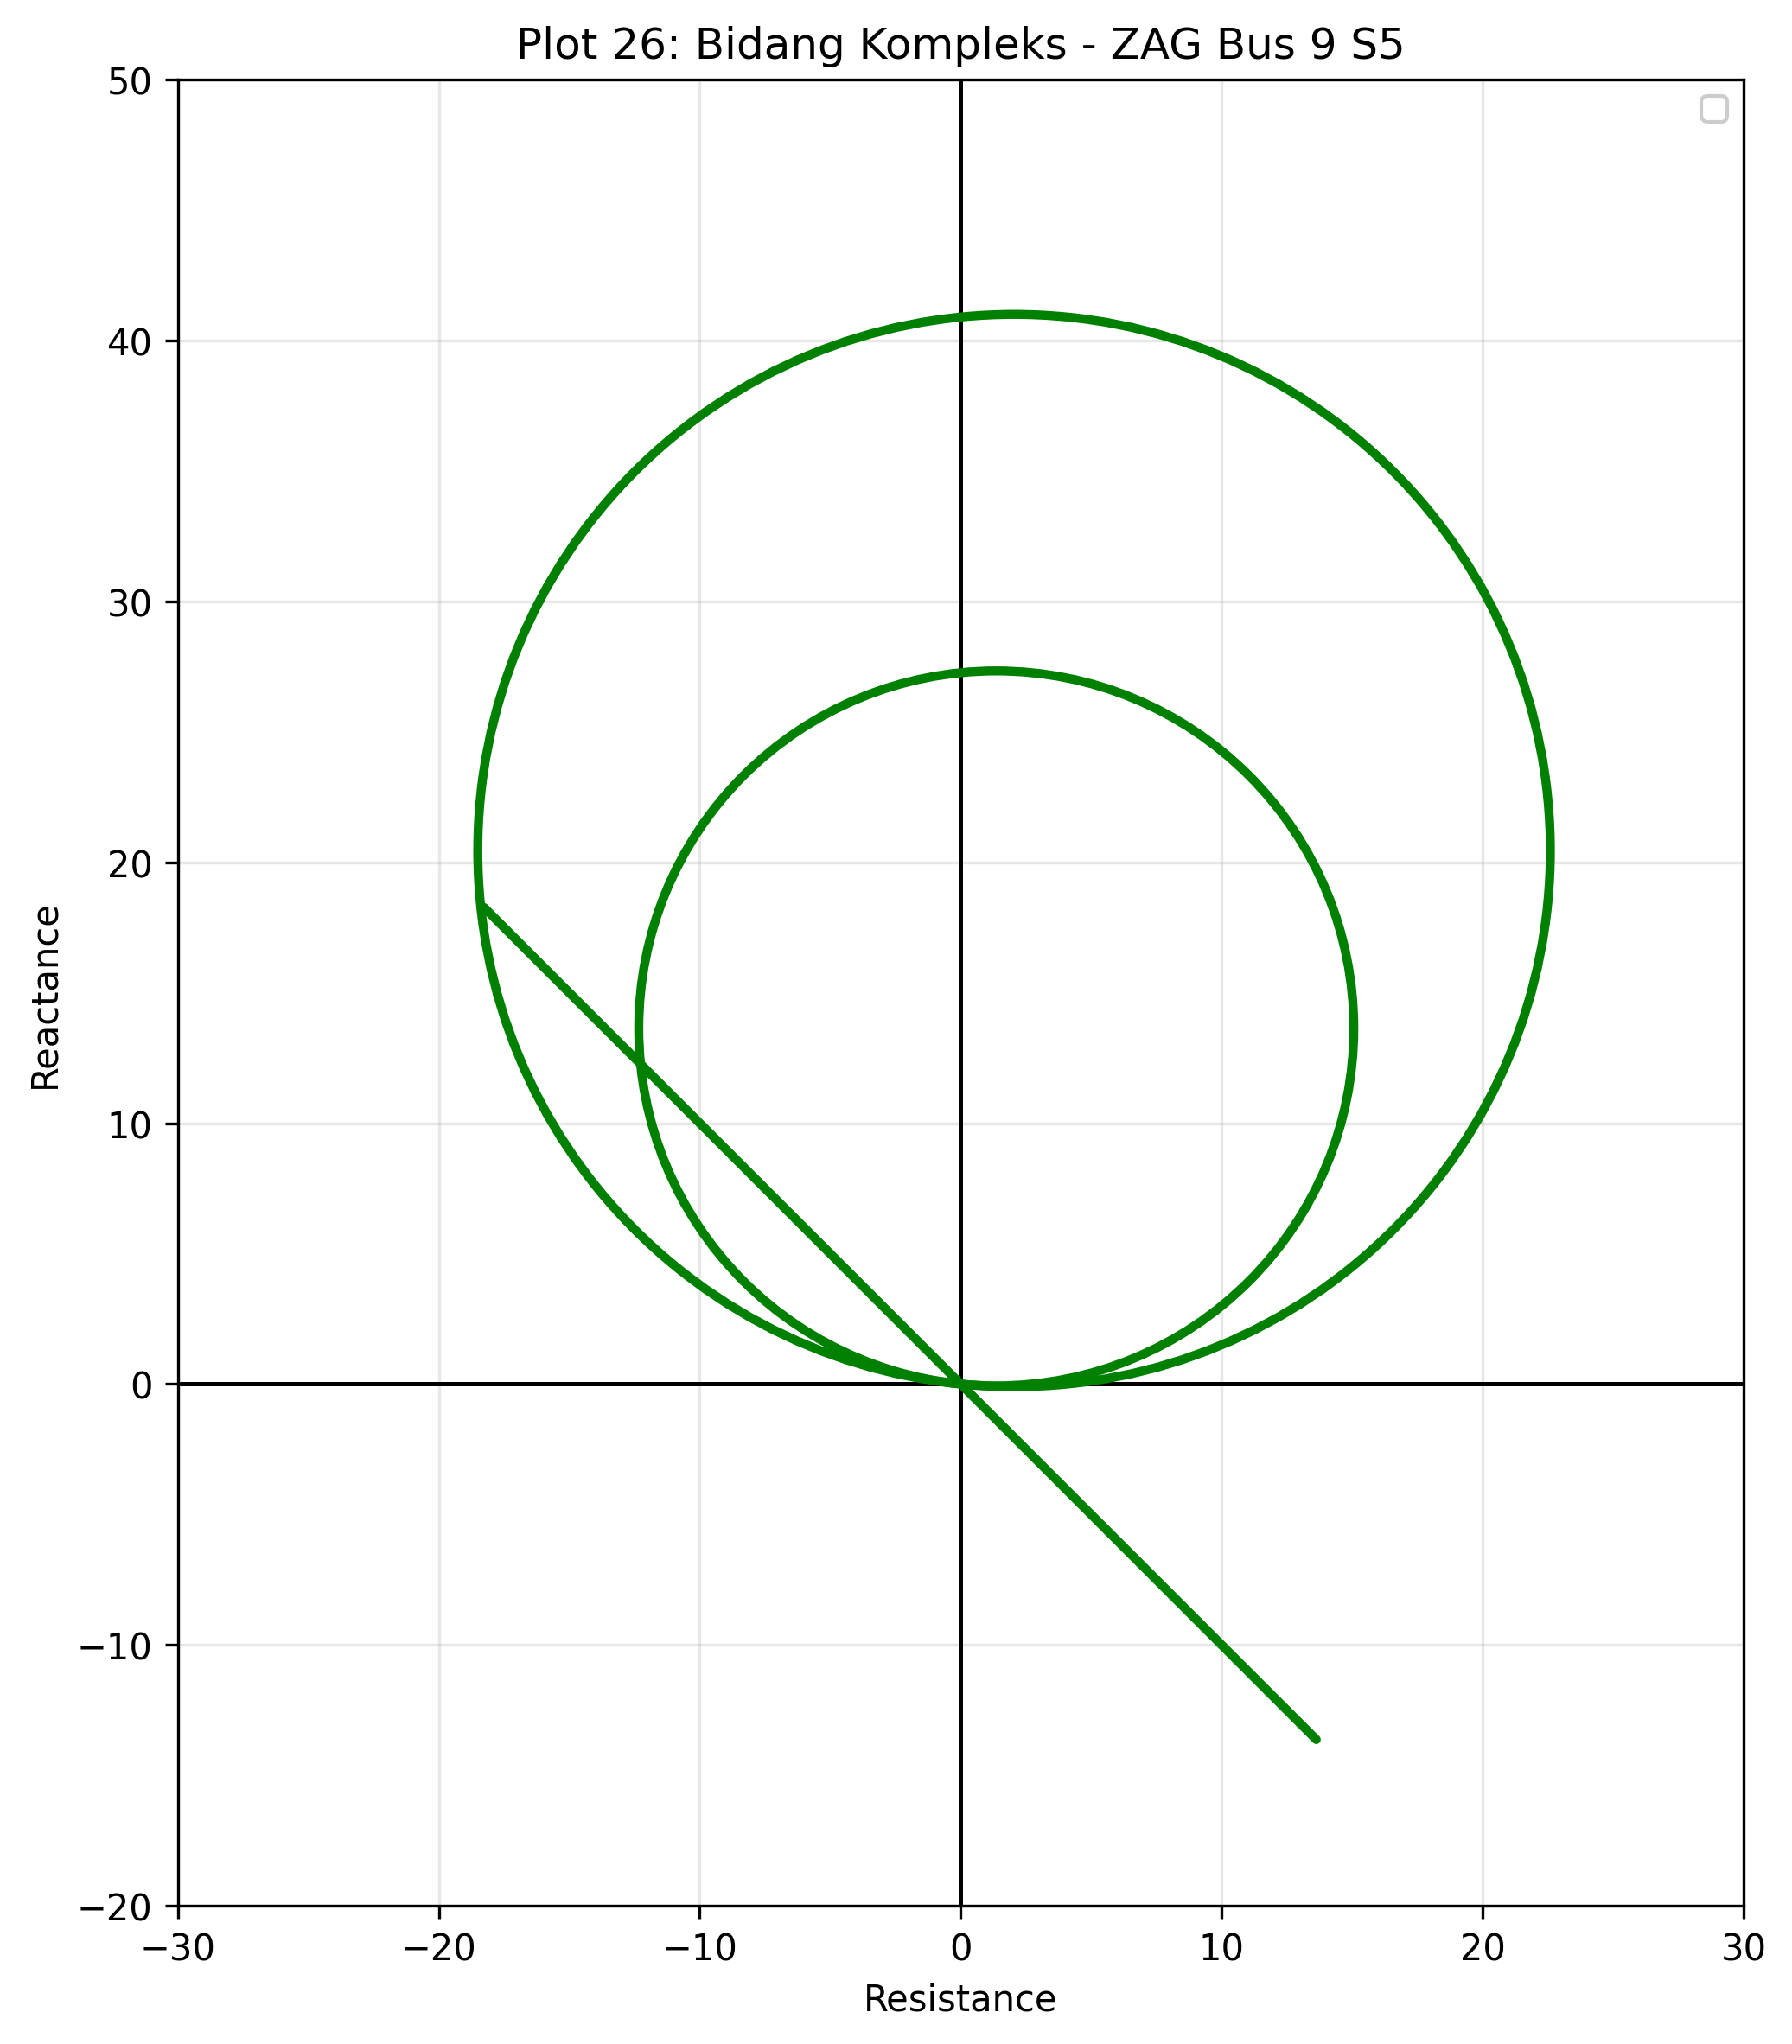
\includegraphics[width=0.8\textwidth]{contents/chapter-4/PRIZI_26_ZAG_Bus_9_S5.png}
%     \caption{Impedansi Tampak ZAG Bus 9 Skenario 5}
%     \label{fig:PRIZI_26_ZAG_Bus_9_S5}
% \end{figure}

\begin{figure}[H]
    \centering

    % Gambar sebelah kiri
    \begin{subfigure}[t]{0.48\textwidth}
        \centering
        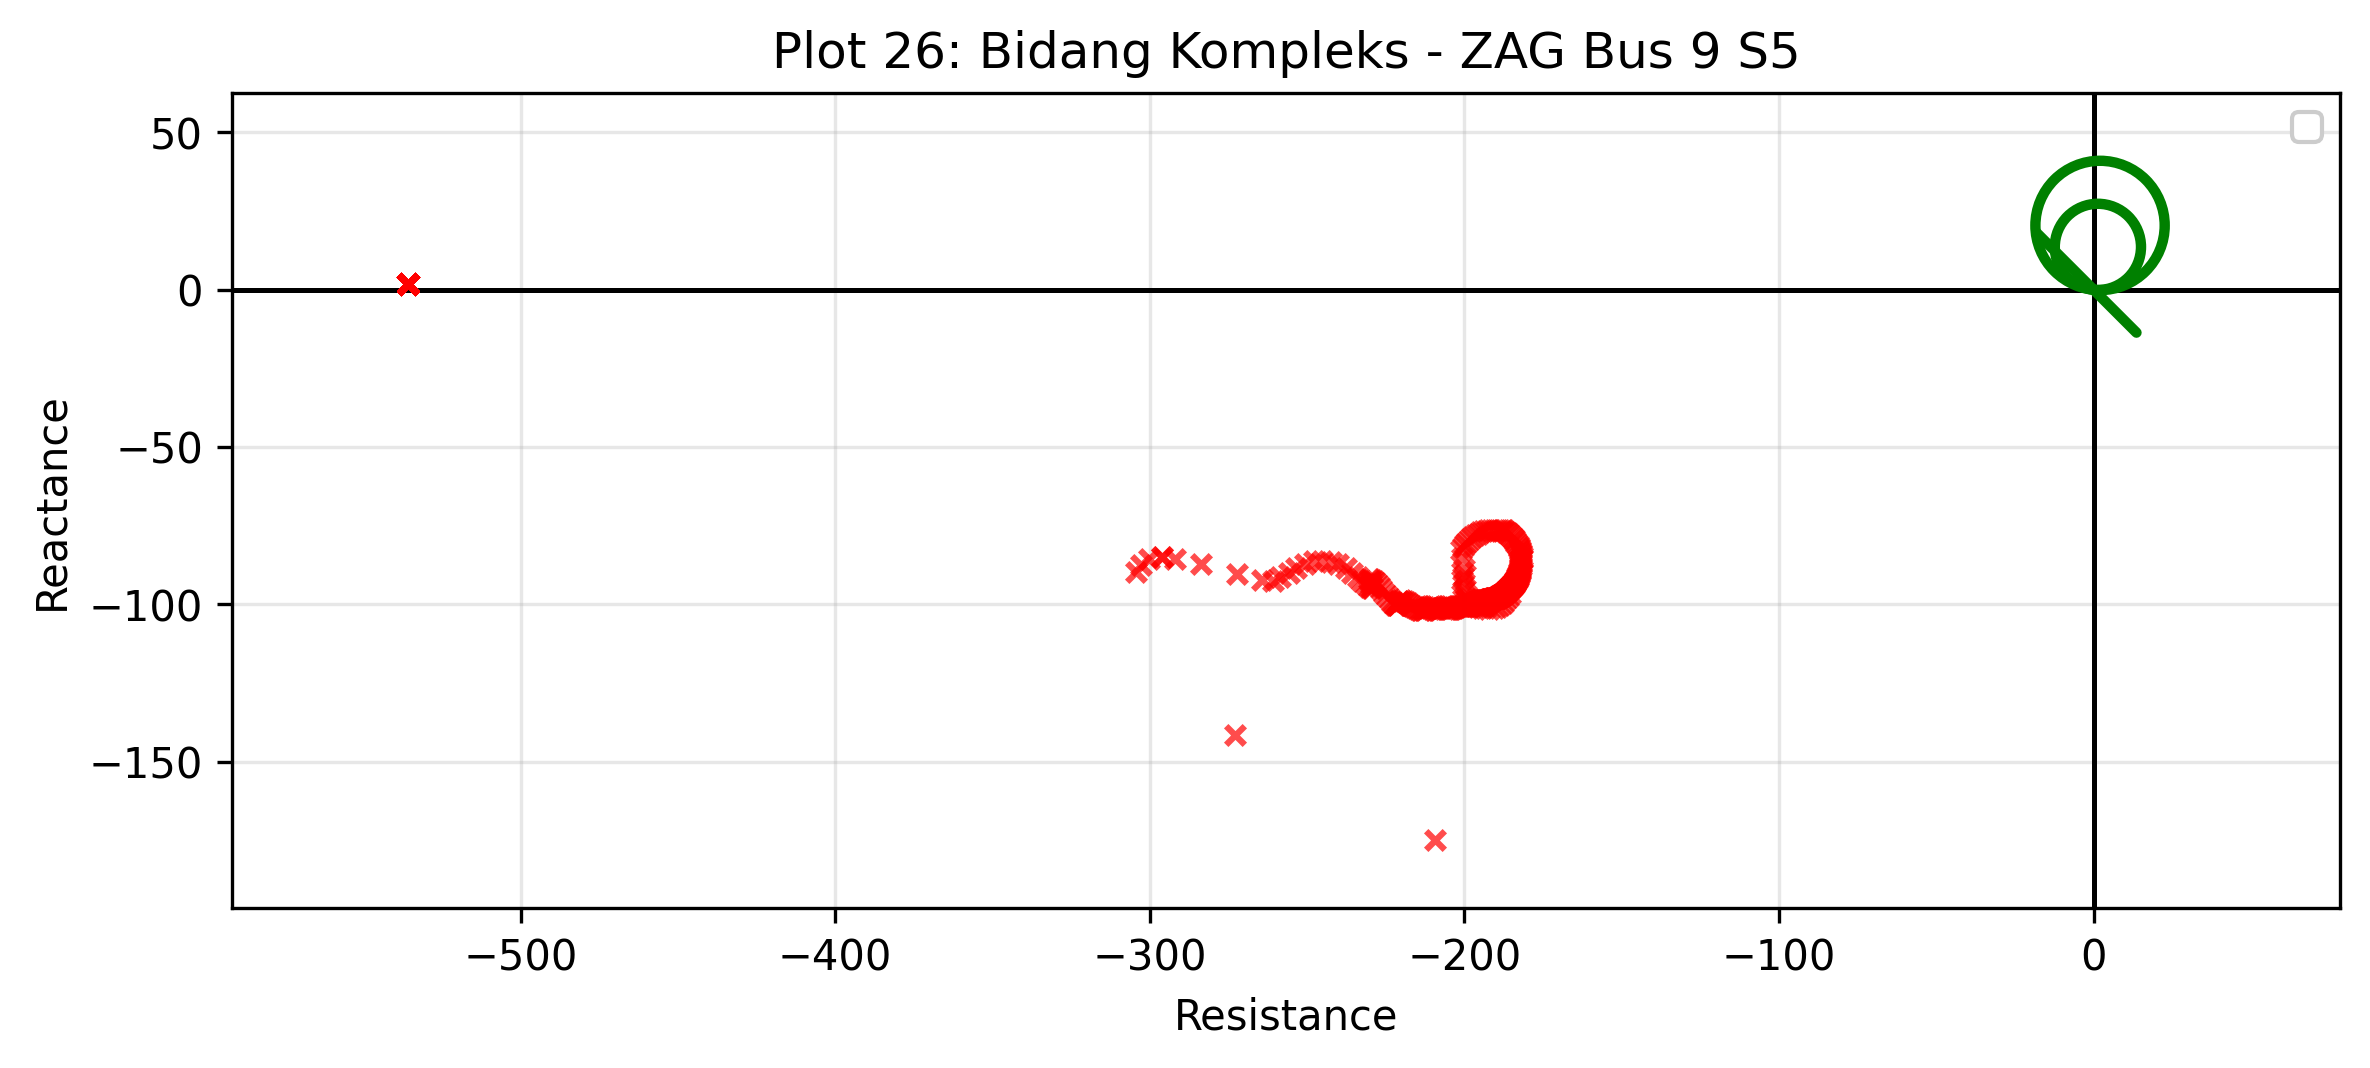
\includegraphics[width=\textwidth]{contents/chapter-4/PRIA_26_ZAG_Bus_9_S5.png}
        \caption{Seluruh Impedansi Tampak}
        \label{fig:PRIA_26_ZAG_Bus_9_S5}
    \end{subfigure}
    \hfill
    % Gambar sebelah kanan
    \begin{subfigure}[t]{0.48\textwidth}
        \centering
        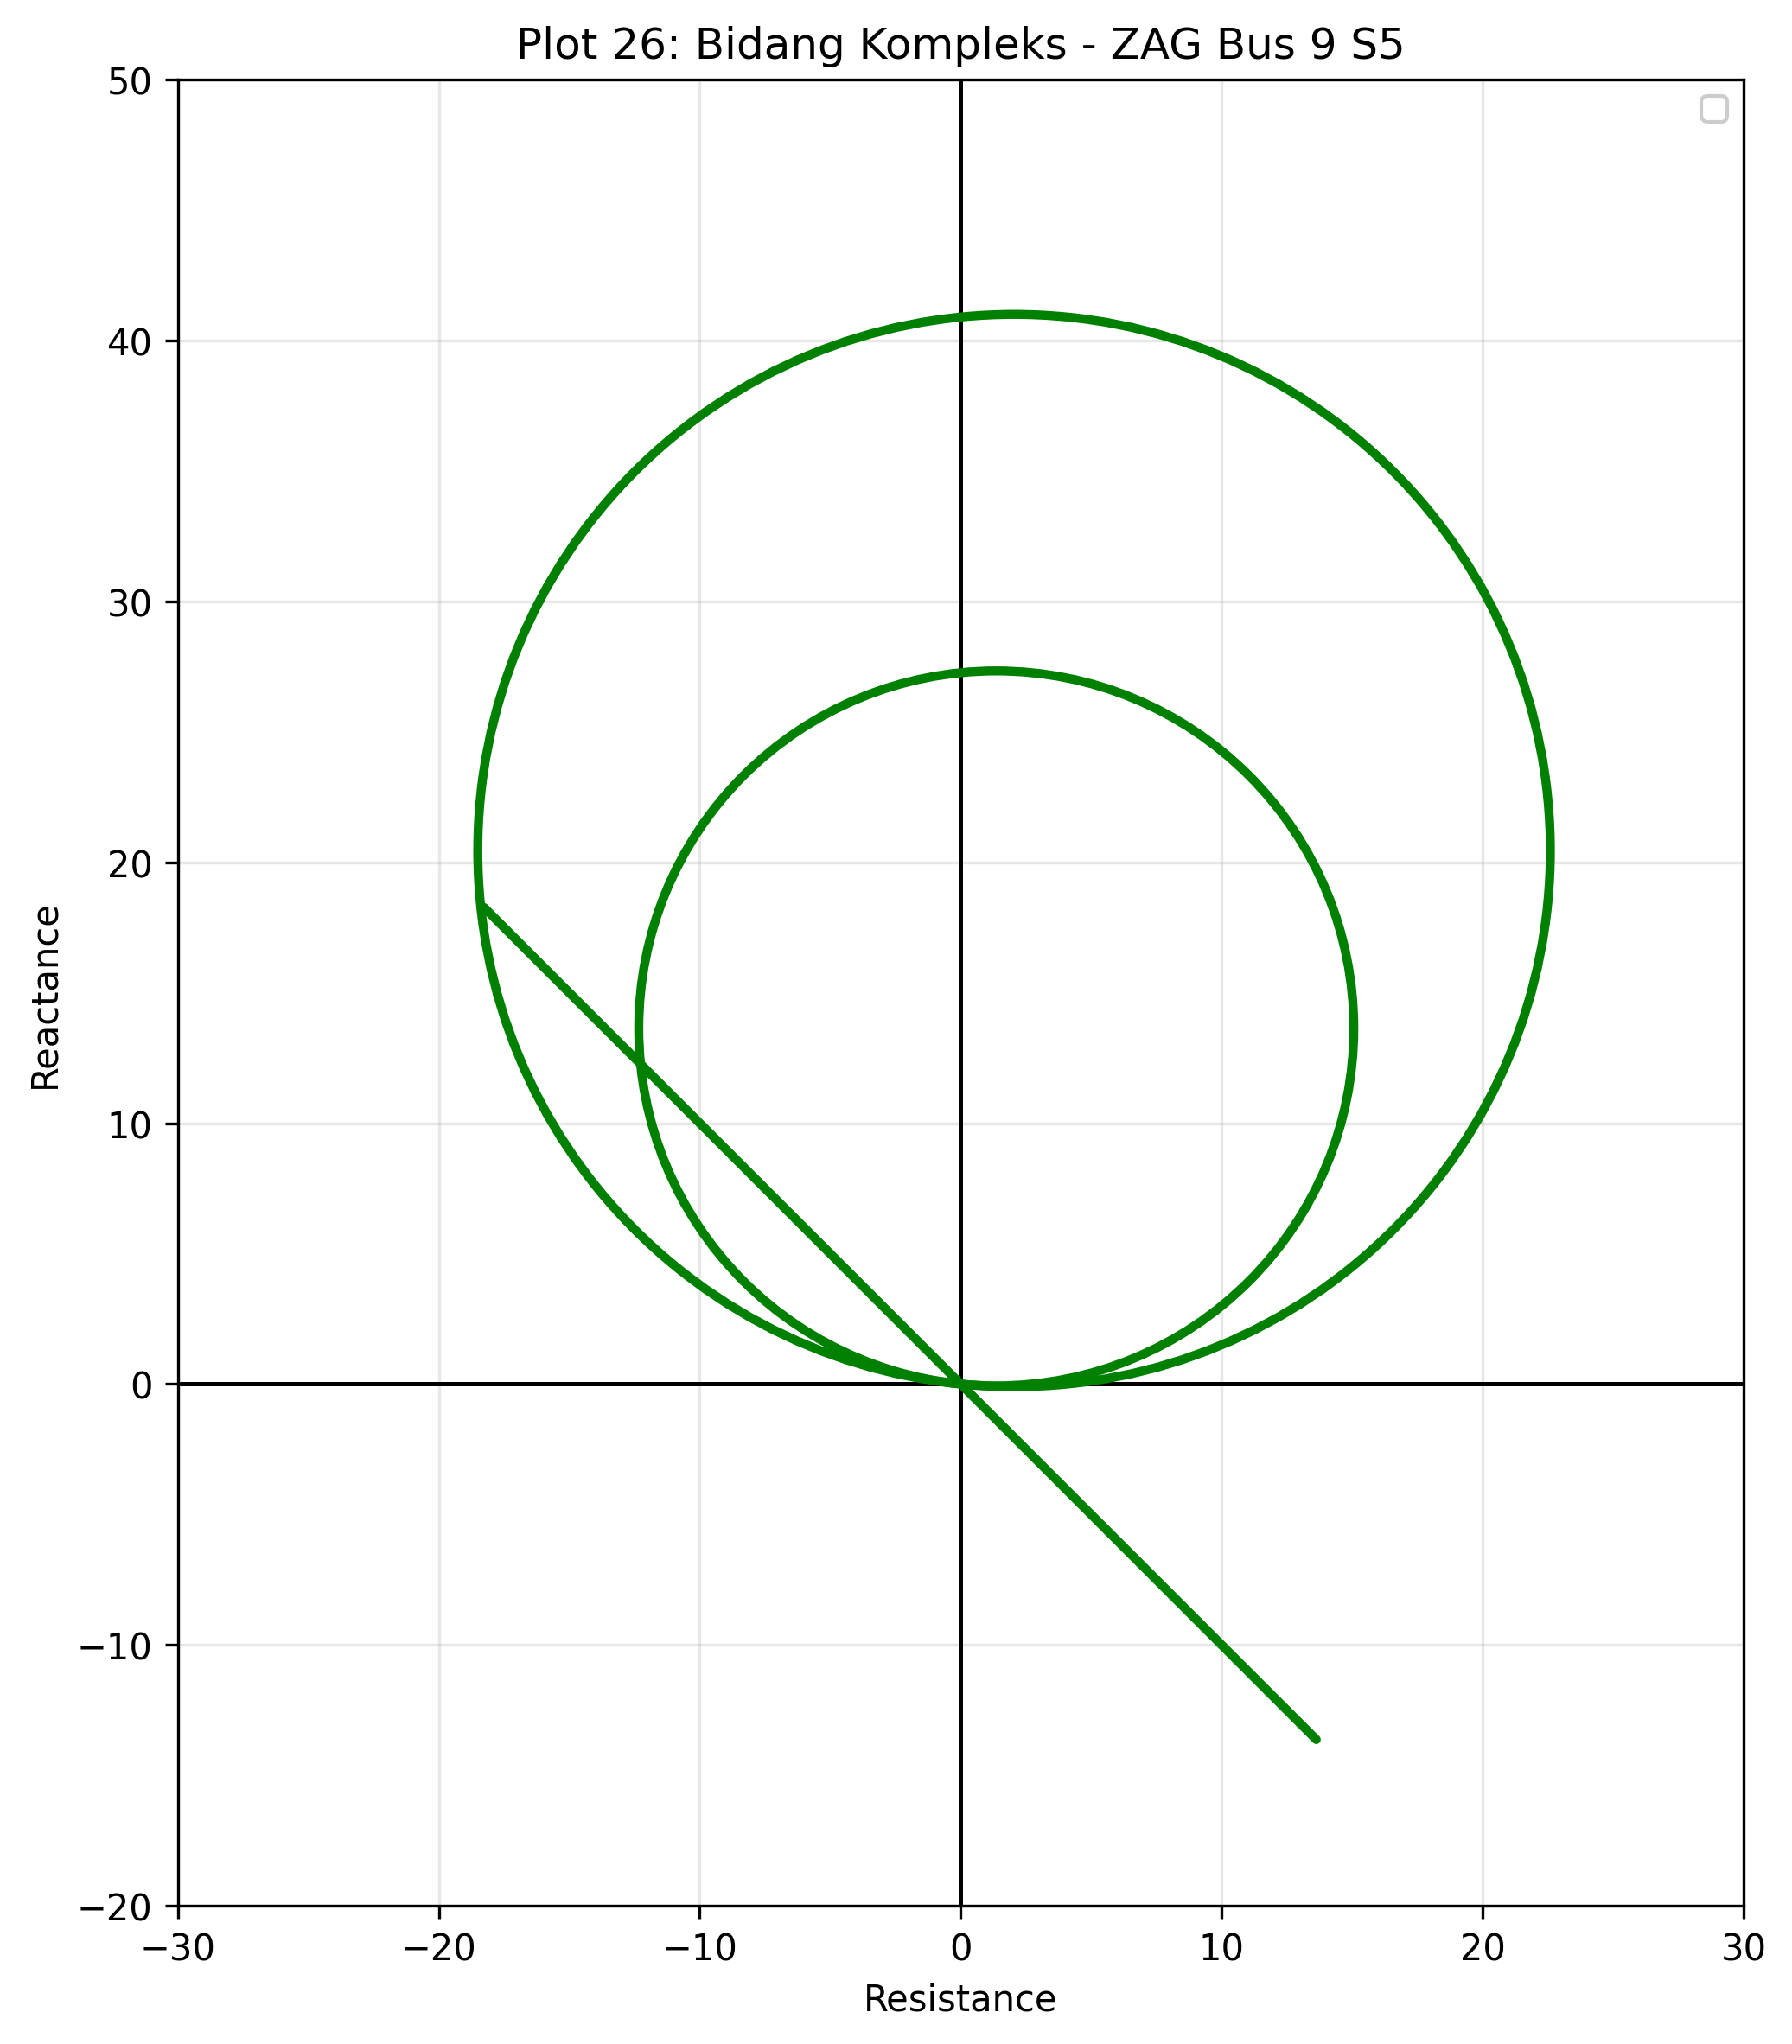
\includegraphics[width=\textwidth]{contents/chapter-4/PRIZI_26_ZAG_Bus_9_S5.png}
        \caption{Zoom In Pada Zona Proteksi}
        \label{fig:PRIZI_26_ZAG_Bus_9_S5}
    \end{subfigure}

    \caption{Impedansi Tampak ZAG Bus 9 Skenario 5}
    \label{fig:Impedansi_Tampak_ZAG_Bus_9_S5}
\end{figure}

Terlihat pada gambar \ref{fig:Impedansi_Tampak_ZAG_Bus_9_S5} bahwa impedansi tampak pada fasa A dengan ground yang dibaca oleh relay 21 sisi bus 9 saat terdapat gangguan bekerja dengan baik sesuai acuan pada \ref{subsec:tanpa_IBR_ex_slg} relay 21 bus 9 tidak mendeteksi adanya gangguan sehingga tidak mengirimkan sinyal trip kepada CB.

%%%%%%%%%%%%%%%%%%%%%%%%%%%%%%%%%%%%%%%%%%%%%%%%%%%%%%%%%%%%%%

% pada skenario 5, impendasi tampak yang dibaca oleh relay 21 pada sisi bus 8 ditunjukkan pada gambar \ref{fig:25_ZAG_Bus_8_S5_dengan_lingkaran_dan_garis} yang menunjukkan bahwa relay bekerja normal pada zona 2. Untuk gambar \ref{fig:26_ZAG_Bus_9_S5_dengan_lingkaran_dan_garis} menunjukkan impedansi tampak yang dibaca oleh relay 21 pada sisi bus 9 dimana terlihat relay tidak trip yang berarti bekerja dengan normal.



\section{Respons Relay 21 pada Sistem dengan WT Type 4}

Bagian ini membahas respons relay 21 ketika jenis IBR diganti menjadi \textit{wind turbine type 4}. Struktur pembahasan dibuat sama dengan bagian sebelumnya agar hasilnya dapat dibandingkan langsung dengan \textit{wind turbine type 3}. Fokus analisis tetap diarahkan pada perubahan impedansi tampak, kondisi \textit{starting} relay, dan keputusan trip pada sisi Bus 8 serta Bus 9.

Skenario yang digunakan pada bagian ini adalah gangguan eksternal DLG pada TL79 dengan kondisi TL78 \textit{out of service}. Hasilnya dibandingkan dengan acuan gangguan eksternal DLG tanpa IBR sehingga dapat dilihat apakah perubahan jenis IBR memengaruhi kecenderungan operasi relay 21.

\subsection{Skenario 2 : Wind Turbine Type 4 External DLG Fault}

Skenario ini digunakan untuk mengevaluasi respons relay 21 ketika sumber IBR yang terhubung ke sistem diganti menjadi \textit{wind turbine type 4}. Karena lokasi dan jenis gangguan yang digunakan adalah gangguan eksternal DLG pada TL79, hasil pada skenario ini dapat dibandingkan dengan acuan kondisi dasar gangguan eksternal DLG serta dengan pola respons pada \textit{wind turbine type 3}.

Dekomposisi komponen urutan arus pada Gambar \ref{fig:decomposition_sequence_current_s2} menjadi penghubung antara karakter kontribusi arus WT Type 4 dan besaran yang dibaca relay pada TL89. Dengan konteks tersebut, pembahasan berikutnya difokuskan pada elemen ZAG, ZBG, dan ZAB dari sisi Bus 8 serta Bus 9 untuk melihat pengaruh arus gangguan terhadap syarat \textit{starting}, posisi impedansi tampak, dan keputusan operasi relay 21.


% pada gambar \ref{fig:07_ZAG_Bus_8_S2_dengan_lingkaran_dan_garis} terlihat untuk titik impedansi tampak ZAG terlihat cukup bergerak dan relay 21 dari sisi bus 8 mengalami over reach pada zona 1 yang seharusnya masuk pada zona 2. pada sisi ini, relay juga mengalami dropout zona 2 yang seharusnya masih dalam jangkauannya.

% Terlihat pada gambar \ref{fig:07_ZAG_Bus_8_S2_dengan_lingkaran_dan_garis} bahwa impedansi tampak pada fasa A dengan ground yang dibaca oleh relay 21 sisi bus 8 saat terdapat gangguan external DLG bekerja dengan acuan pada \ref{subsec:tanpa_IBR_in_dlg} relay 21 bus 8 mengalami misoperation karena mendeteksi adanya gangguan namun overreach pada zona 1 yang seharusnya pada zona 2 serta mengalami dropout pada zona 2 dan memberikan sinyal trip kepada CB pada zona 2.

%%%%%%%%%%%%%%%%%%%%%%%%%%%%%%%%%SISI PRIMER%%%%%%%%%%%%%%%%%%%%%%%%%%%%%%%%%%

\begin{figure}[H]
    \centering
    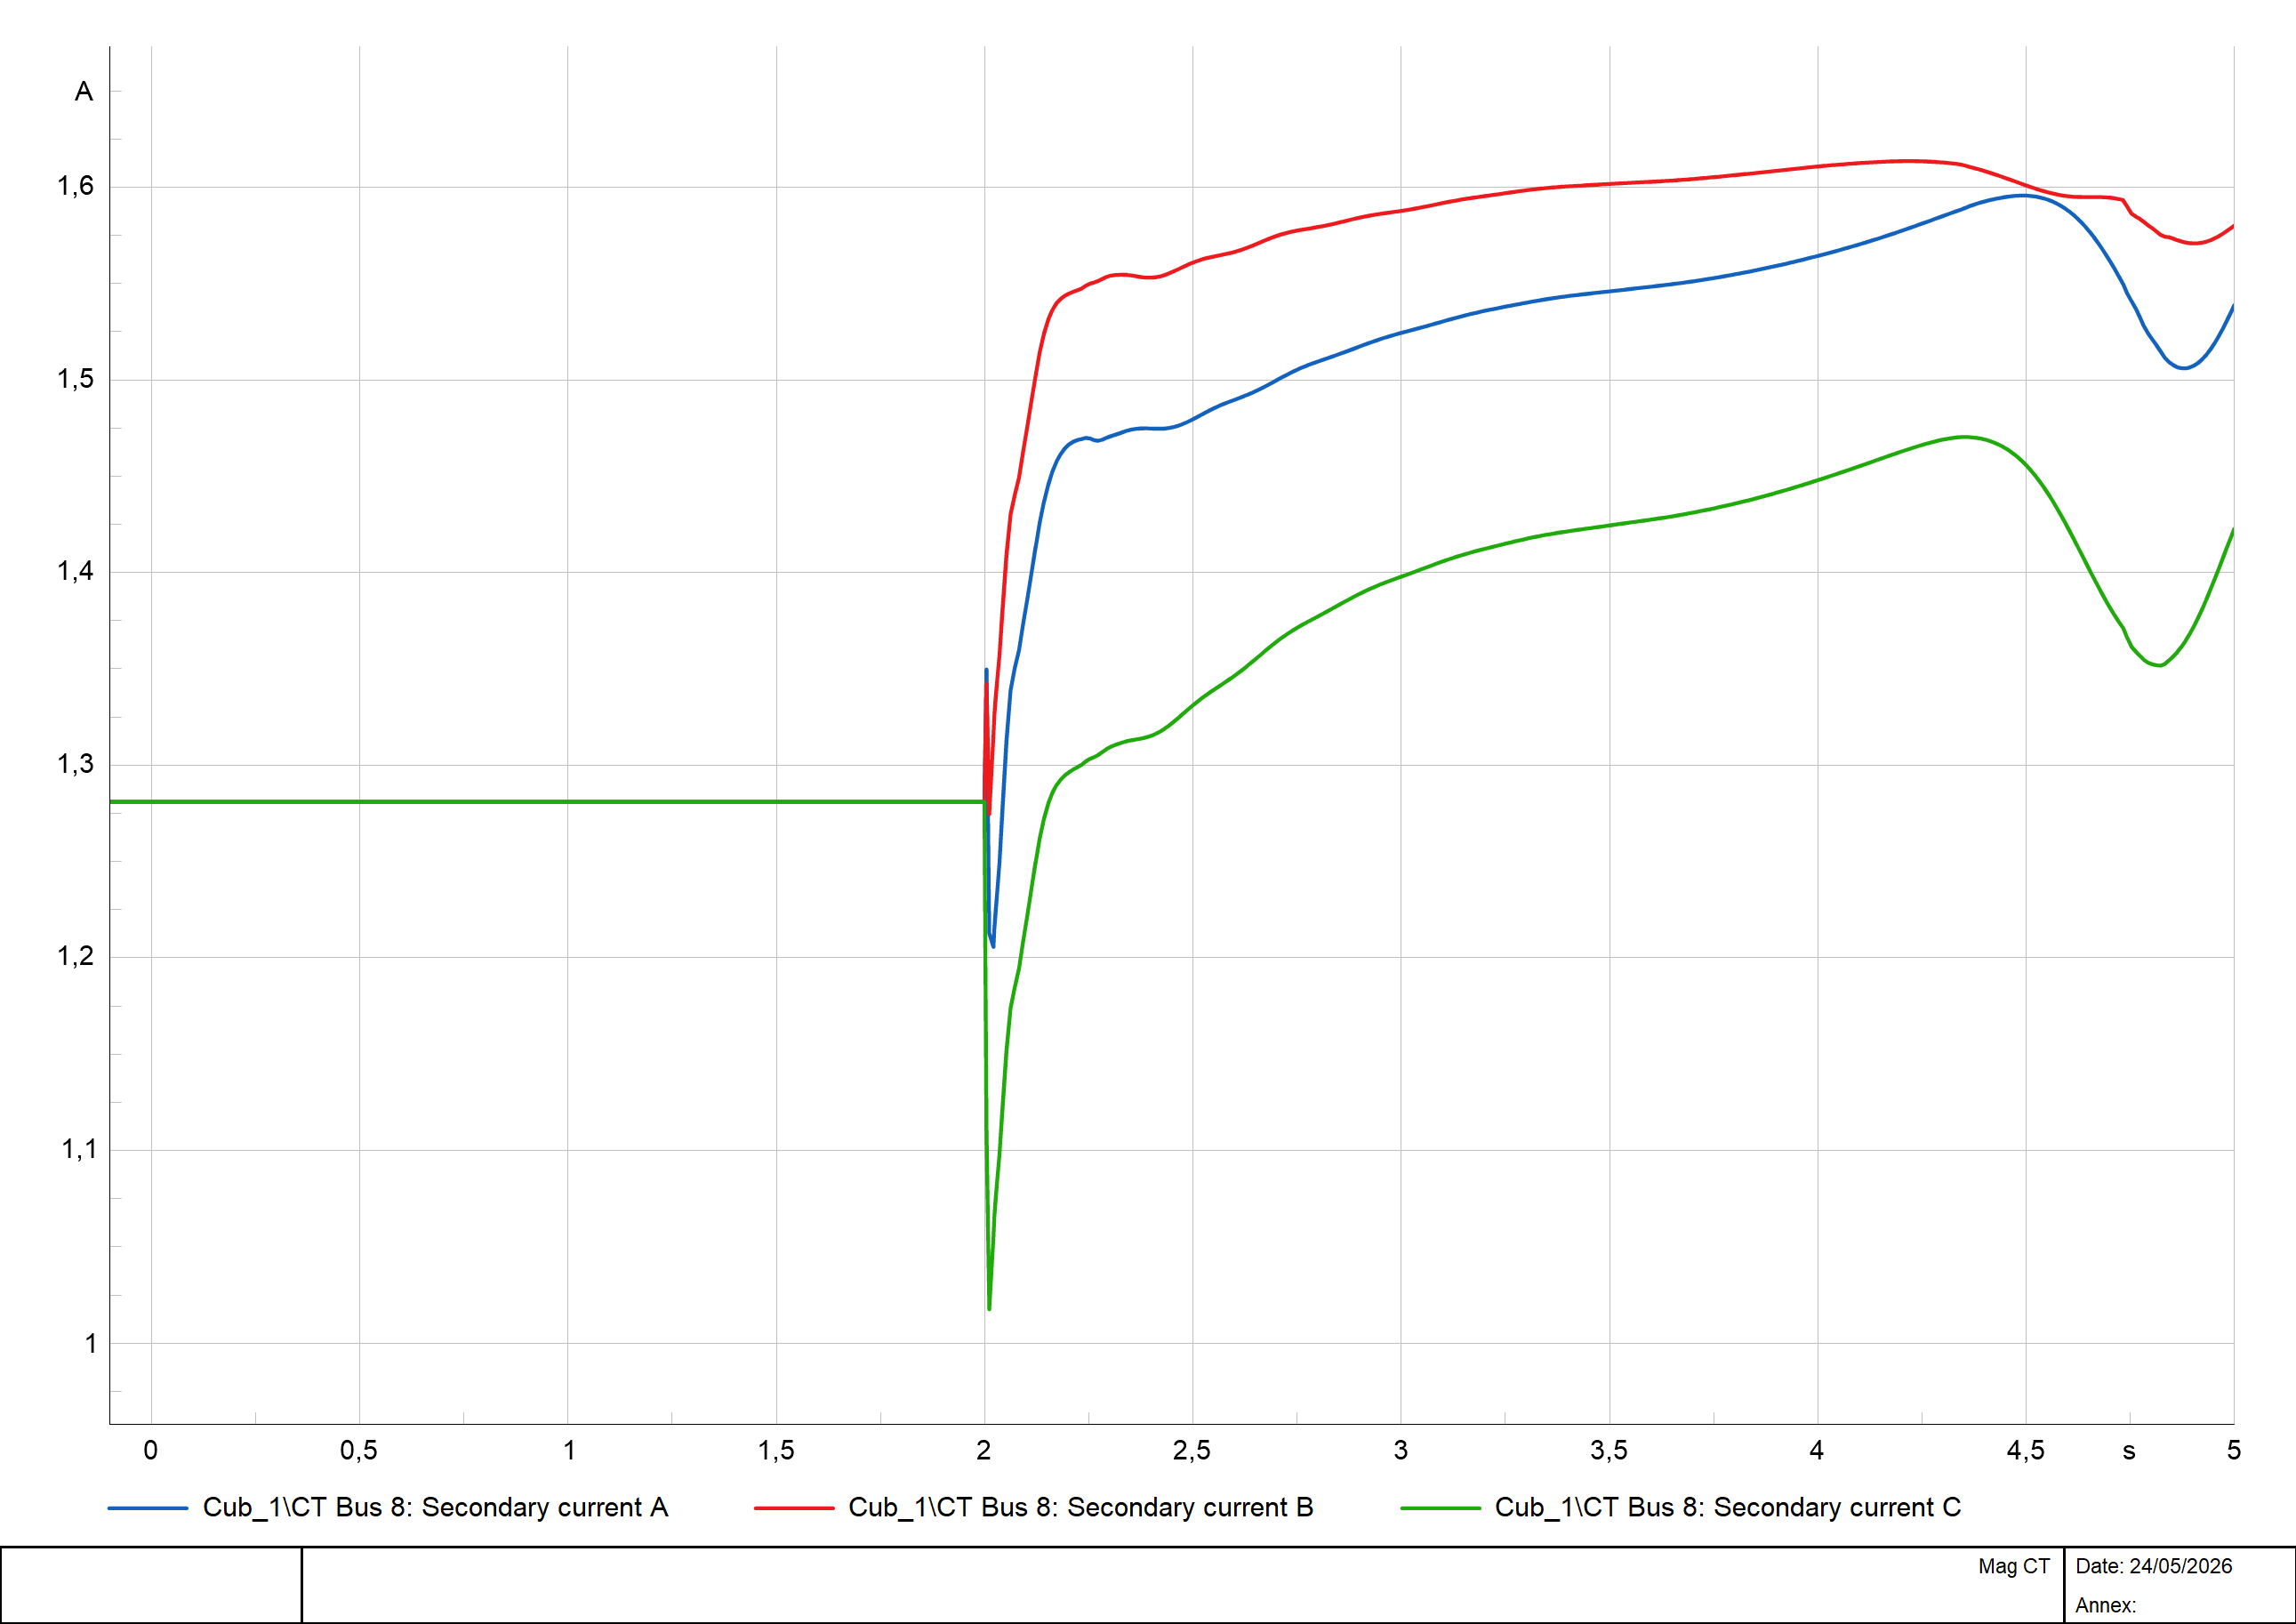
\includegraphics[width=0.8\textwidth]{contents/chapter-4/Bus_8_Ex_DLG_S2.png}
    \caption{Arus Sekunder CT Bus 8 Skenario 2}
    \label{fig:Bus_8_Ex_DLG_S2}
\end{figure}

Gambar \ref{fig:Bus_8_Ex_DLG_S2} menunjukkan arus sekunder CT pada Bus 8 untuk skenario 2 saat terjadi gangguan eksternal DLG. Sebelum gangguan, arus pada ketiga fasa berada pada nilai 1,281 A sekunder. Setelah gangguan terjadi, arus fasa A meningkat menjadi 1,6 A sekunder atau 1,25 p.u., arus fasa B meningkat menjadi 1,613 A sekunder atau 1,26 p.u., dan arus fasa C meningkat menjadi 1,47 A sekunder atau 1,15 p.u. Kenaikan arus tersebut menunjukkan adanya perubahan arus saat gangguan, tetapi nilainya masih belum memenuhi arus minimum yang diperlukan untuk membuat relay 21 sisi Bus 8 aktif.

\begin{figure}[H]
    \centering

    % Gambar sebelah kiri
    \begin{subfigure}[t]{0.48\textwidth}
        \centering
        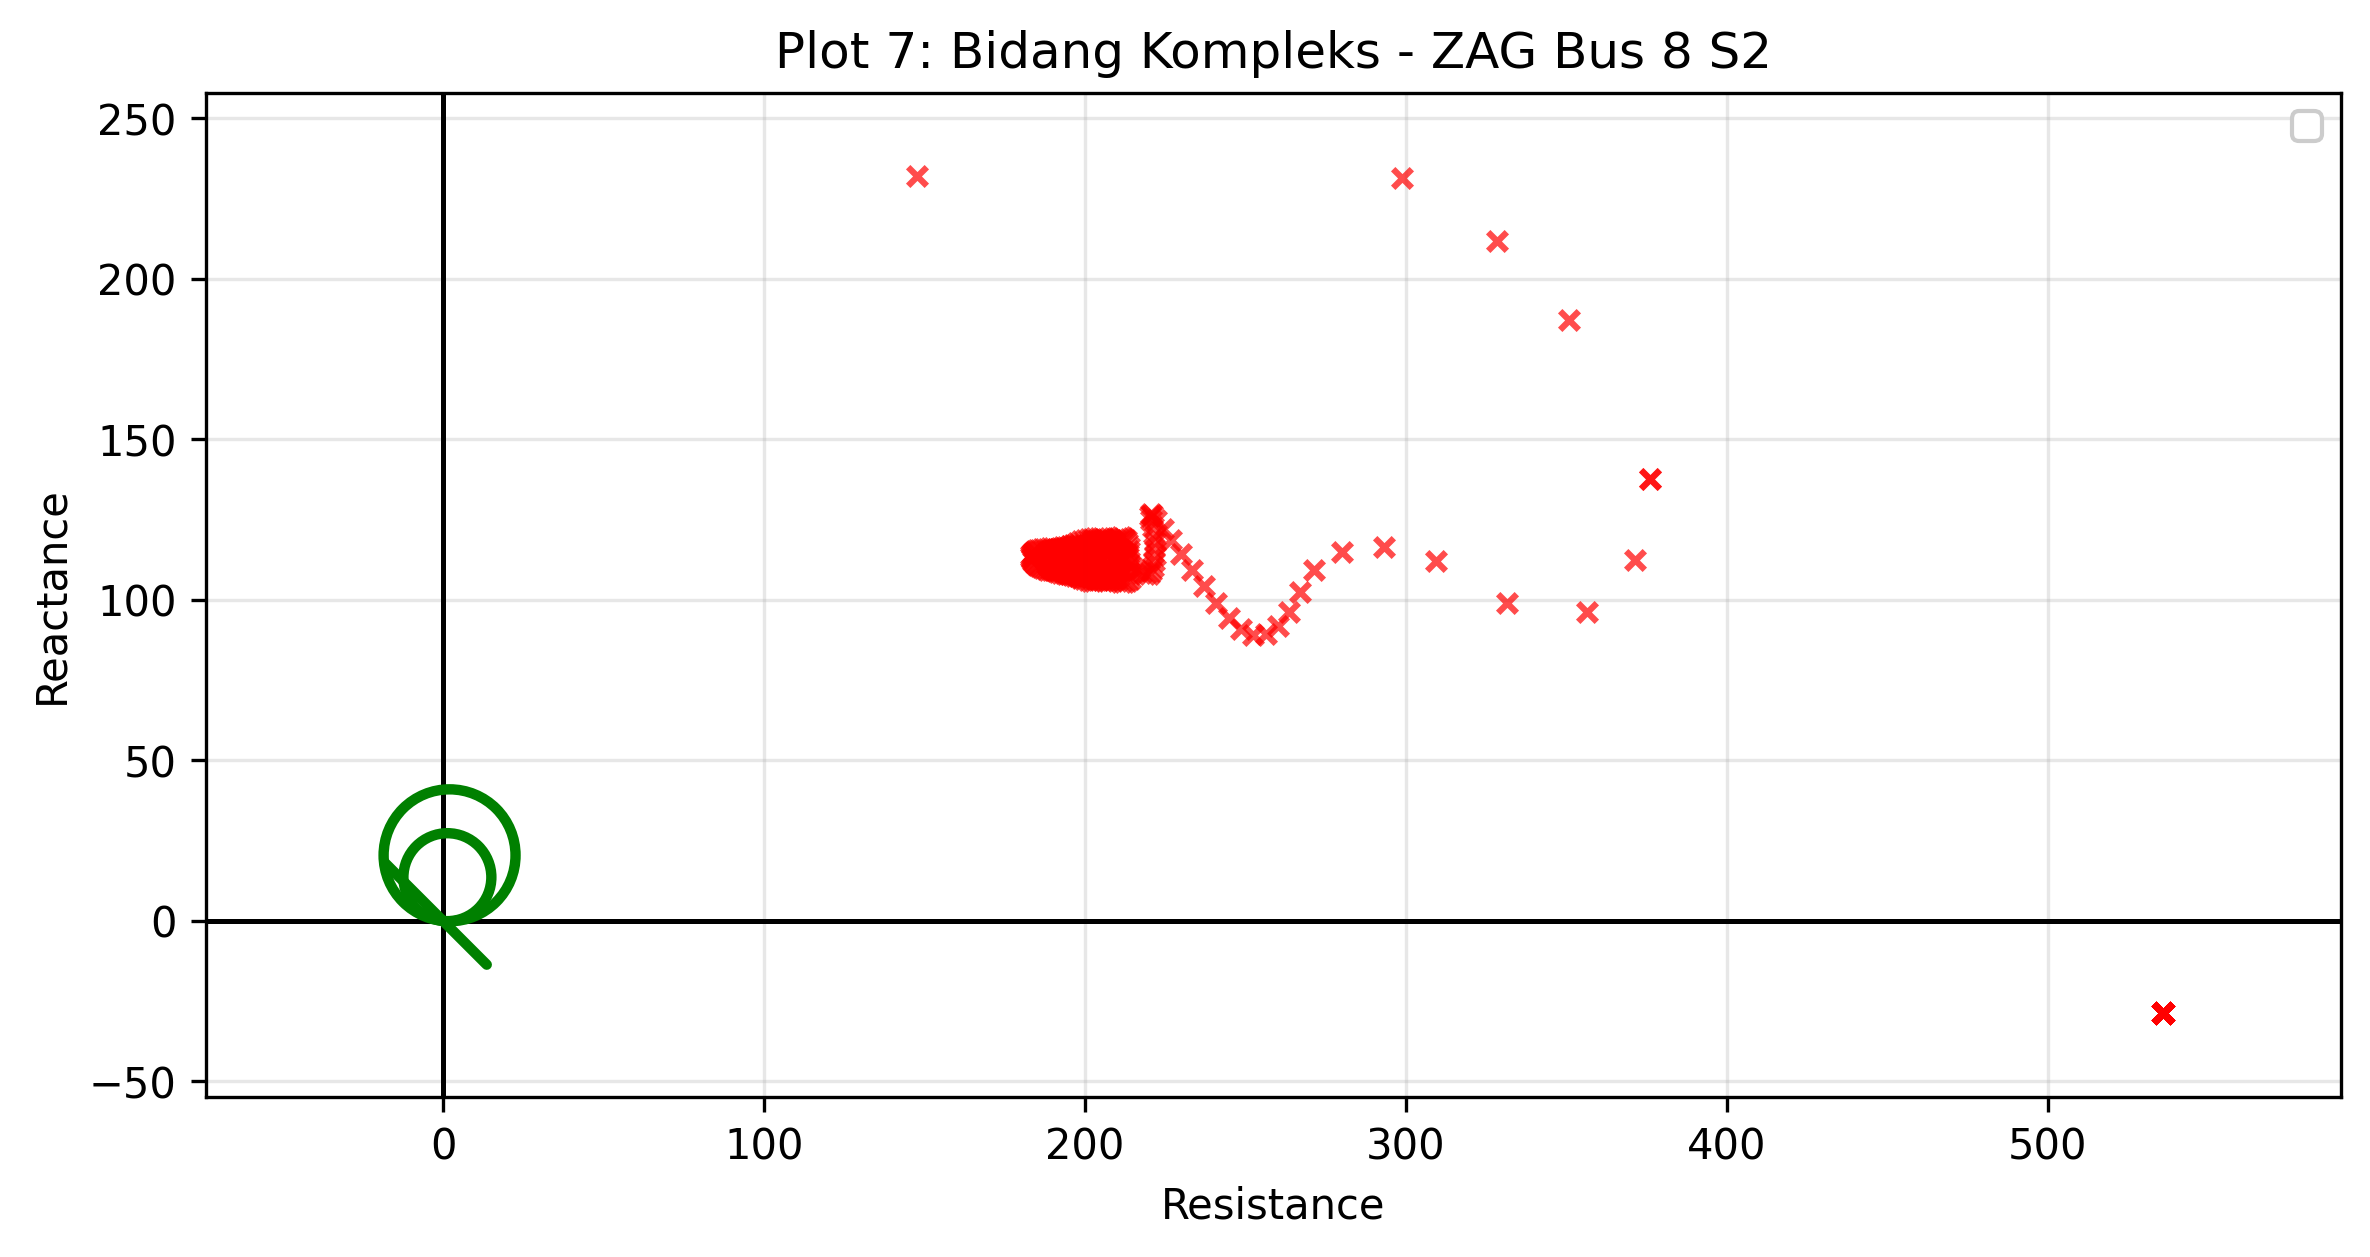
\includegraphics[width=\textwidth]{contents/chapter-4/PRIA_07_ZAG_Bus_8_S2.png}
        \caption{Seluruh Impedansi Tampak}
        \label{fig:PRIA_07_ZAG_Bus_8_S2}
    \end{subfigure}
    \hfill
    % Gambar sebelah kanan
    \begin{subfigure}[t]{0.48\textwidth}
        \centering
        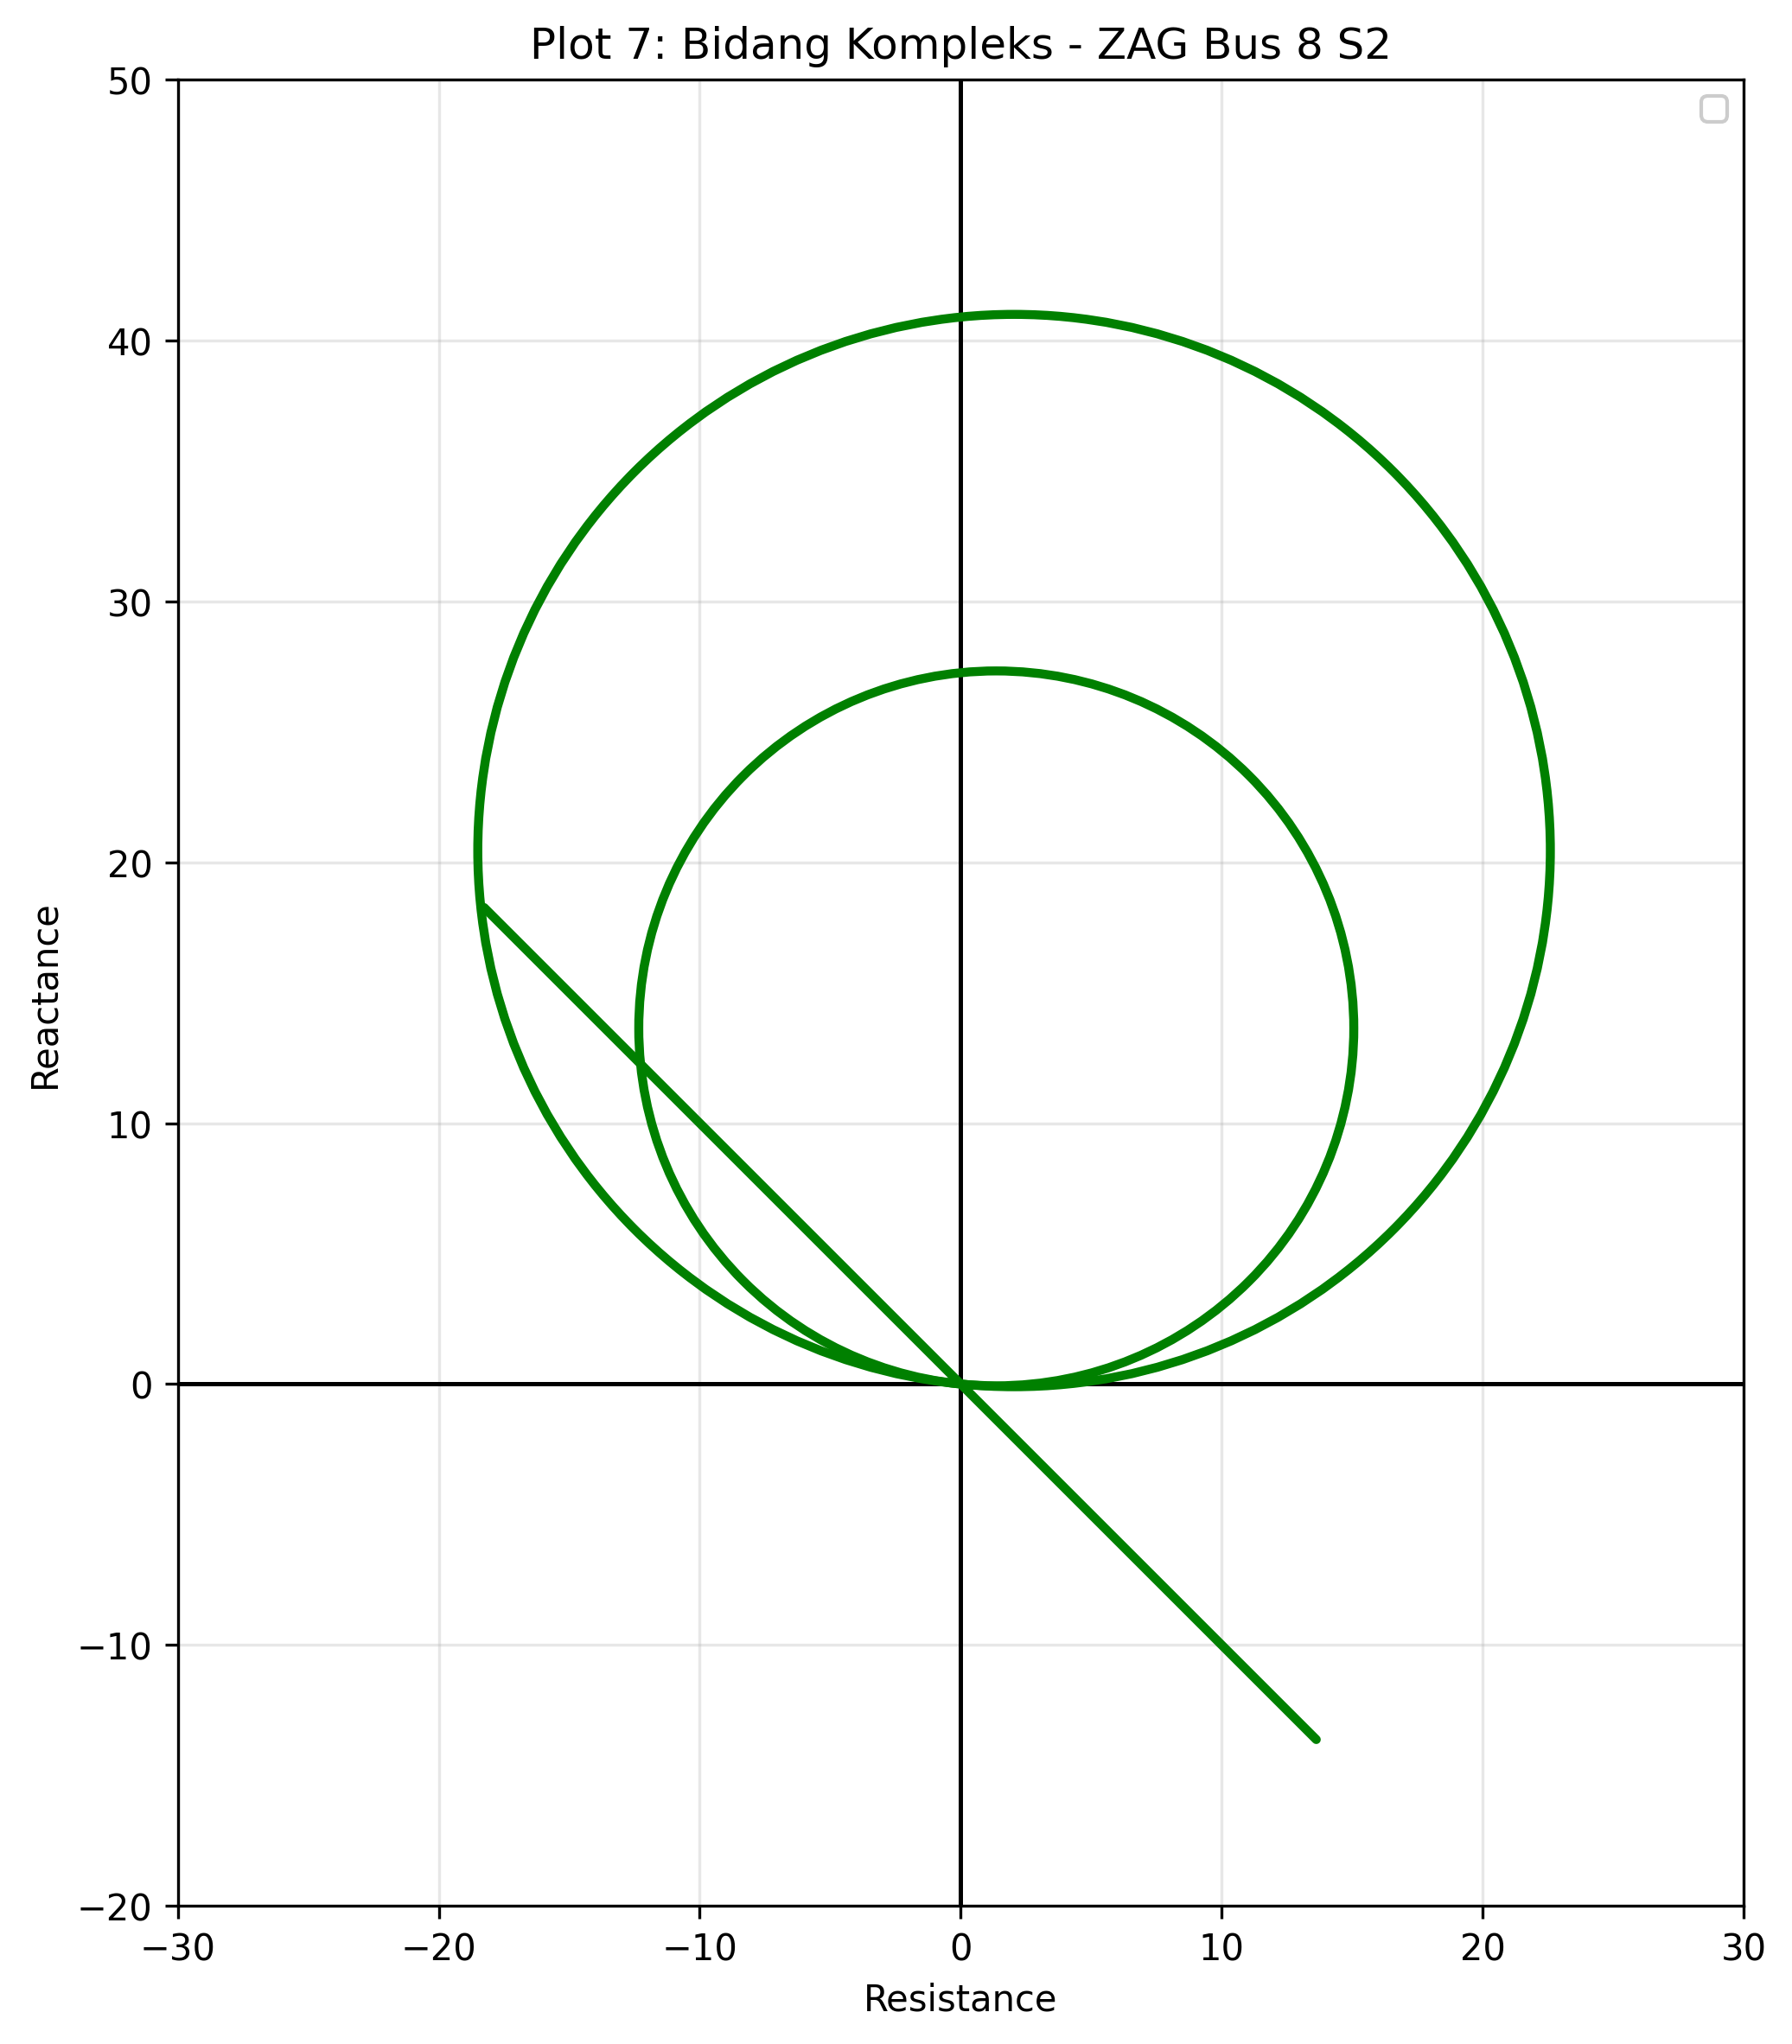
\includegraphics[width=\textwidth]{contents/chapter-4/PRIZI_07_ZAG_Bus_8_S2.png}
        \caption{Zoom In Pada Zona Proteksi}
        \label{fig:PRIZI_07_ZAG_Bus_8_S2}
    \end{subfigure}

    \caption{Impedansi Tampak ZAG Bus 8 Skenario 2}
    \label{fig:Impedansi_Tampak_ZAG_Bus_8_S2}
\end{figure}

Gambar \ref{fig:Impedansi_Tampak_ZAG_Bus_8_S2} menunjukkan bahwa impedansi tampak loop fasa A dengan ground yang dibaca oleh relay 21 sisi Bus 8 tidak masuk ke dalam zona proteksi. Kondisi ini sejalan dengan pembacaan arus sekunder CT pada Gambar \ref{fig:Bus_8_Ex_DLG_S2}, karena arus gangguan yang terbaca masih cukup kecil dan belum memenuhi syarat \textit{starting} untuk membuat relay aktif. Dengan mengacu pada kondisi dasar gangguan eksternal DLG pada Subbab \ref{subsec:tanpa_IBR_ex_dlg}, respons relay 21 sisi Bus 8 pada elemen ini dikategorikan mengalami \textit{misoperation}.

%%%%%%%%%%%%%%%%%%%%%%%%%%%%%%%%%%%%%%%%%%%%%%%%%%%%%%%%%%%%%%

% \begin{figure}[H]
%     \centering
%     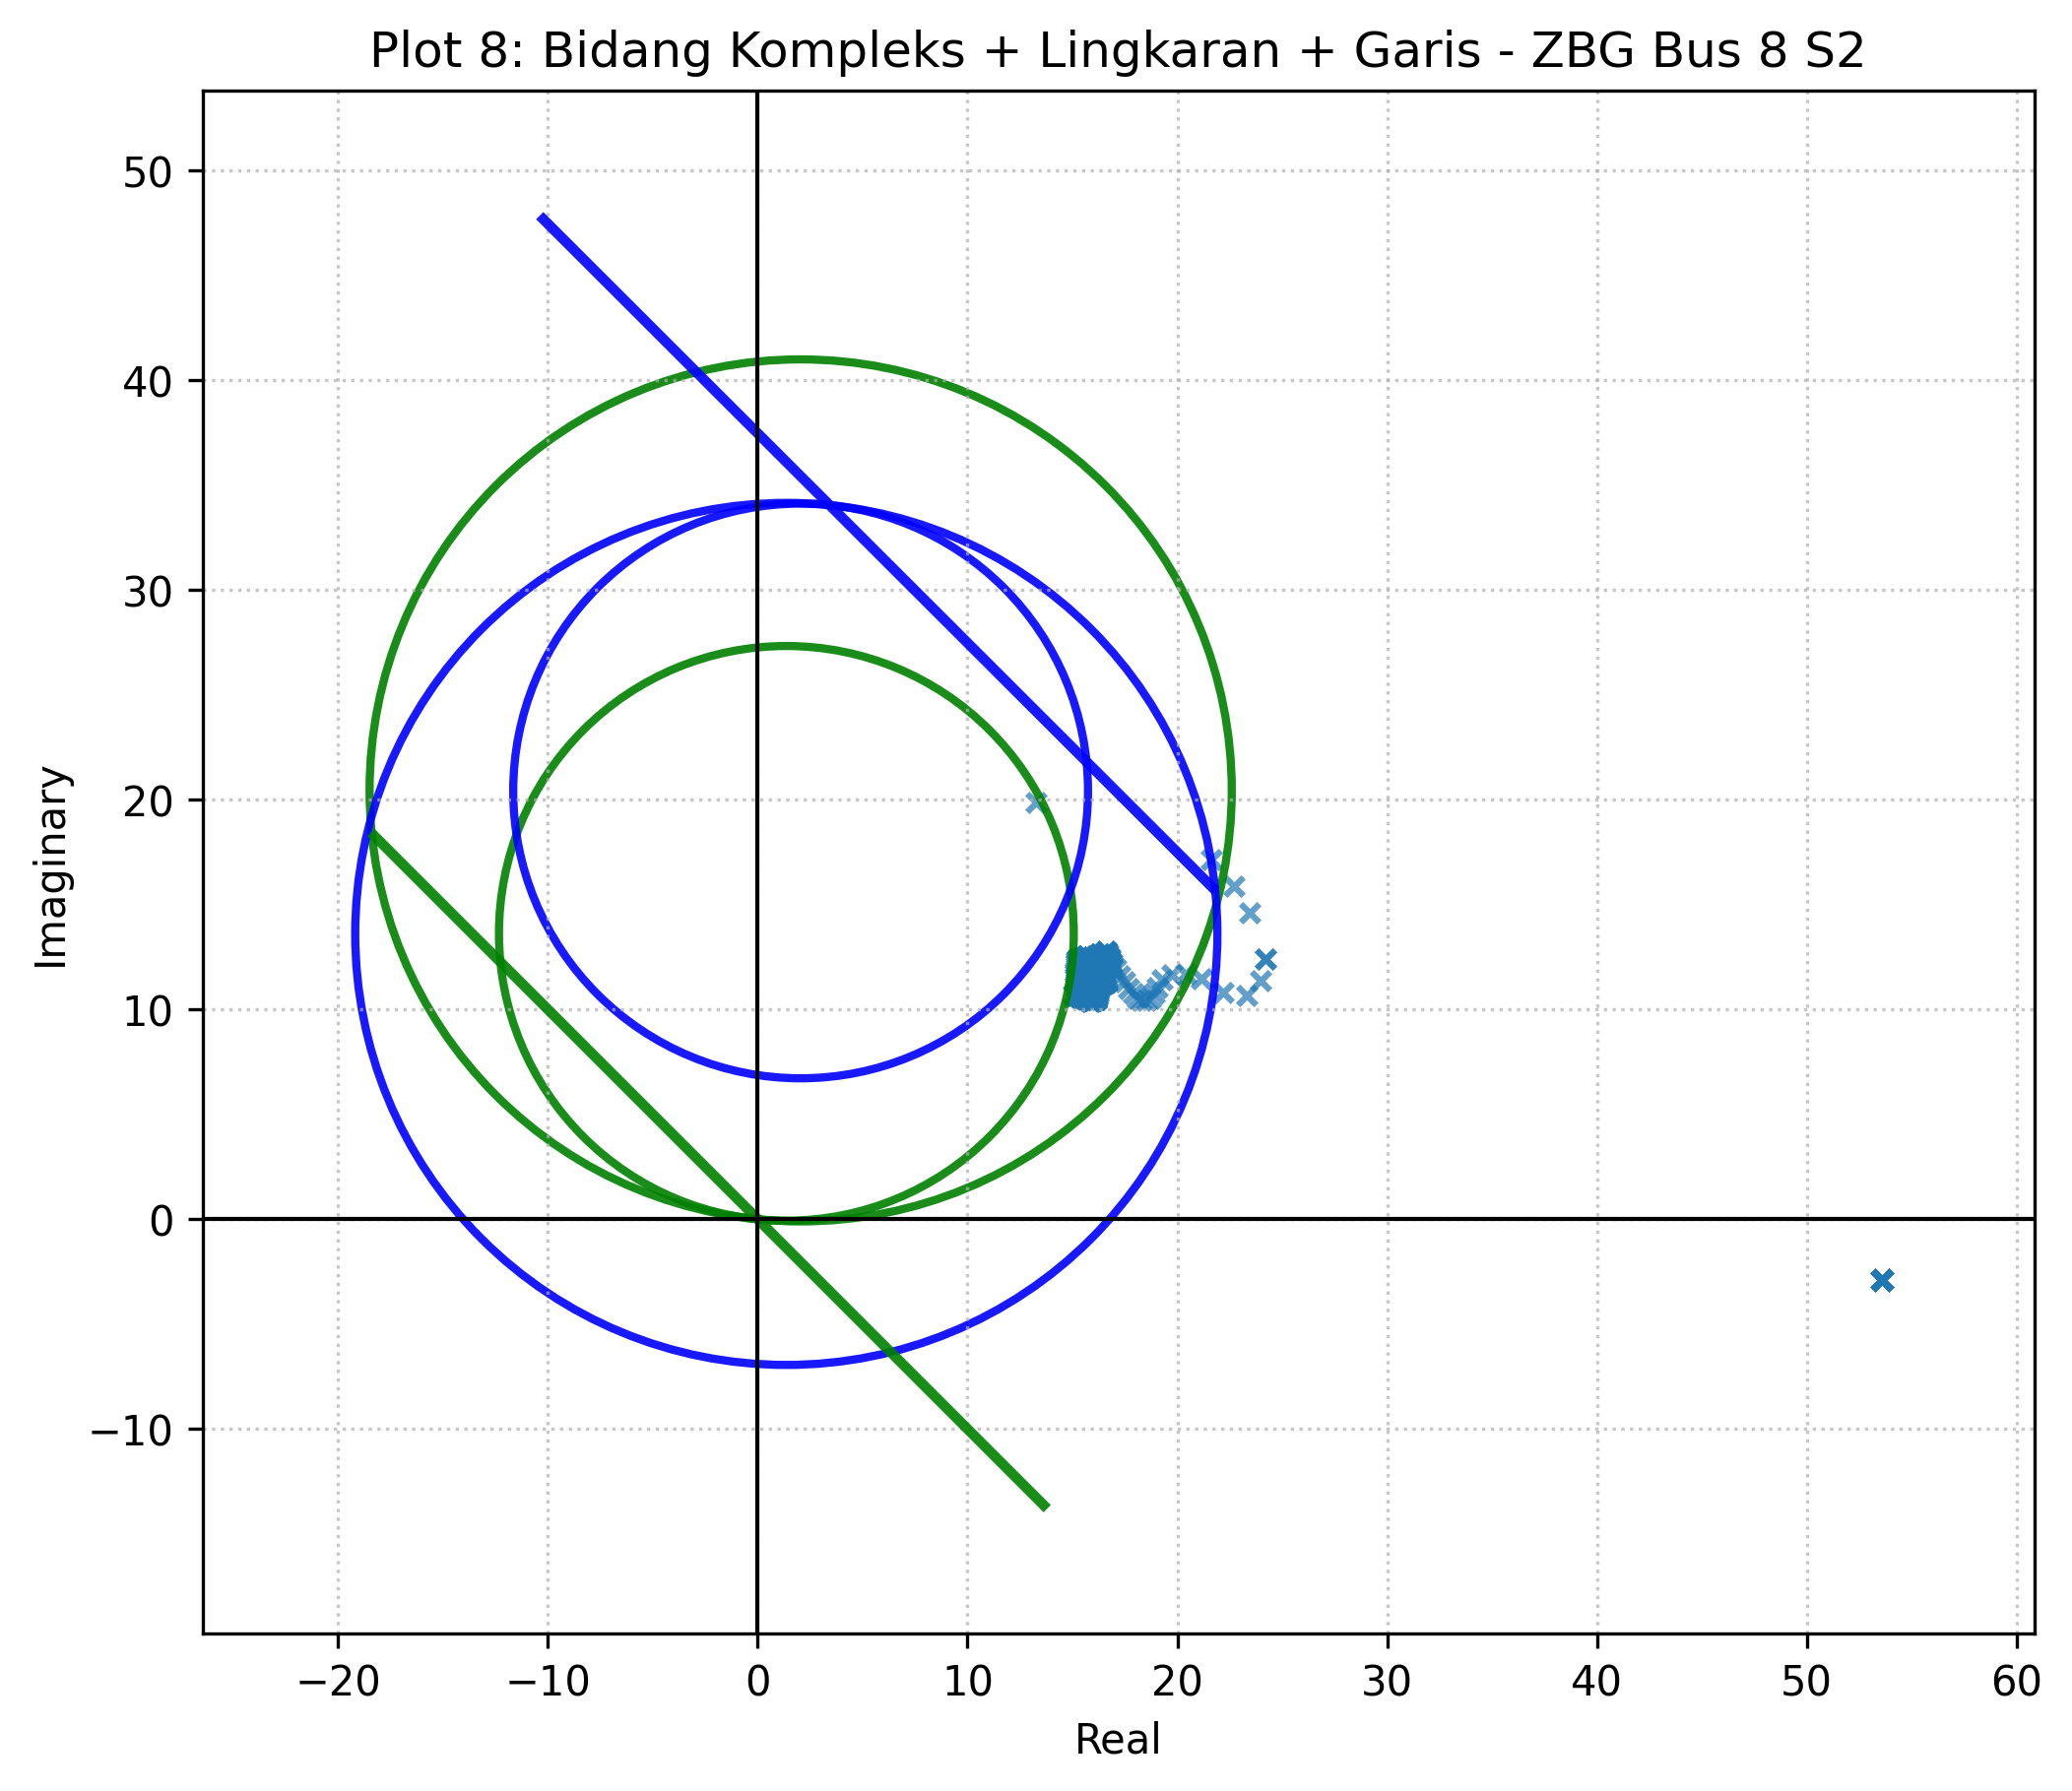
\includegraphics[width=0.8\textwidth]{contents/chapter-4/08_ZBG_Bus_8_S2_dengan_lingkaran_dan_garis.png}
%     \caption{Impedansi Tampak ZBG Bus 8 Skenario 2}
%     \label{fig:08_ZBG_Bus_8_S2_dengan_lingkaran_dan_garis}
% \end{figure}

% untuk pada gambar \ref{fig:08_ZBG_Bus_8_S2_dengan_lingkaran_dan_garis} memiliki fenomena yang saya dengan gambar \ref{fig:07_ZAG_Bus_8_S2_dengan_lingkaran_dan_garis} dimana terlihat untuk titik impedansi tampak ZBG terlihat cukup bergerak dan relay 21 dari sisi bus 8 mengalami over reach pada zona 1 yang seharusnya masuk pada zona 2. pada sisi ini, relay juga mengalami dropout zona 2 yang seharusnya masih dalam jangkauannya.

% Terlihat pada gambar \ref{fig:08_ZBG_Bus_8_S2_dengan_lingkaran_dan_garis} bahwa impedansi tampak pada fasa B dengan ground yang dibaca oleh relay 21 sisi bus 8 saat terdapat gangguan external DLG bekerja dengan acuan pada \ref{subsec:tanpa_IBR_in_dlg} relay 21 bus 8 mengalami misoperation karena mendeteksi adanya gangguan namun overreach pada zona 1 yang seharusnya pada zona 2 serta mengalami dropout pada zona 2 dan memberikan sinyal trip kepada CB pada zona 2

%%%%%%%%%%%%%%%%%%%%%%%%%%%%%%%%%SISI PRIMER%%%%%%%%%%%%%%%%%%%%%%%%%%%%%%%%%%

% \begin{figure}[H]
%     \centering
%     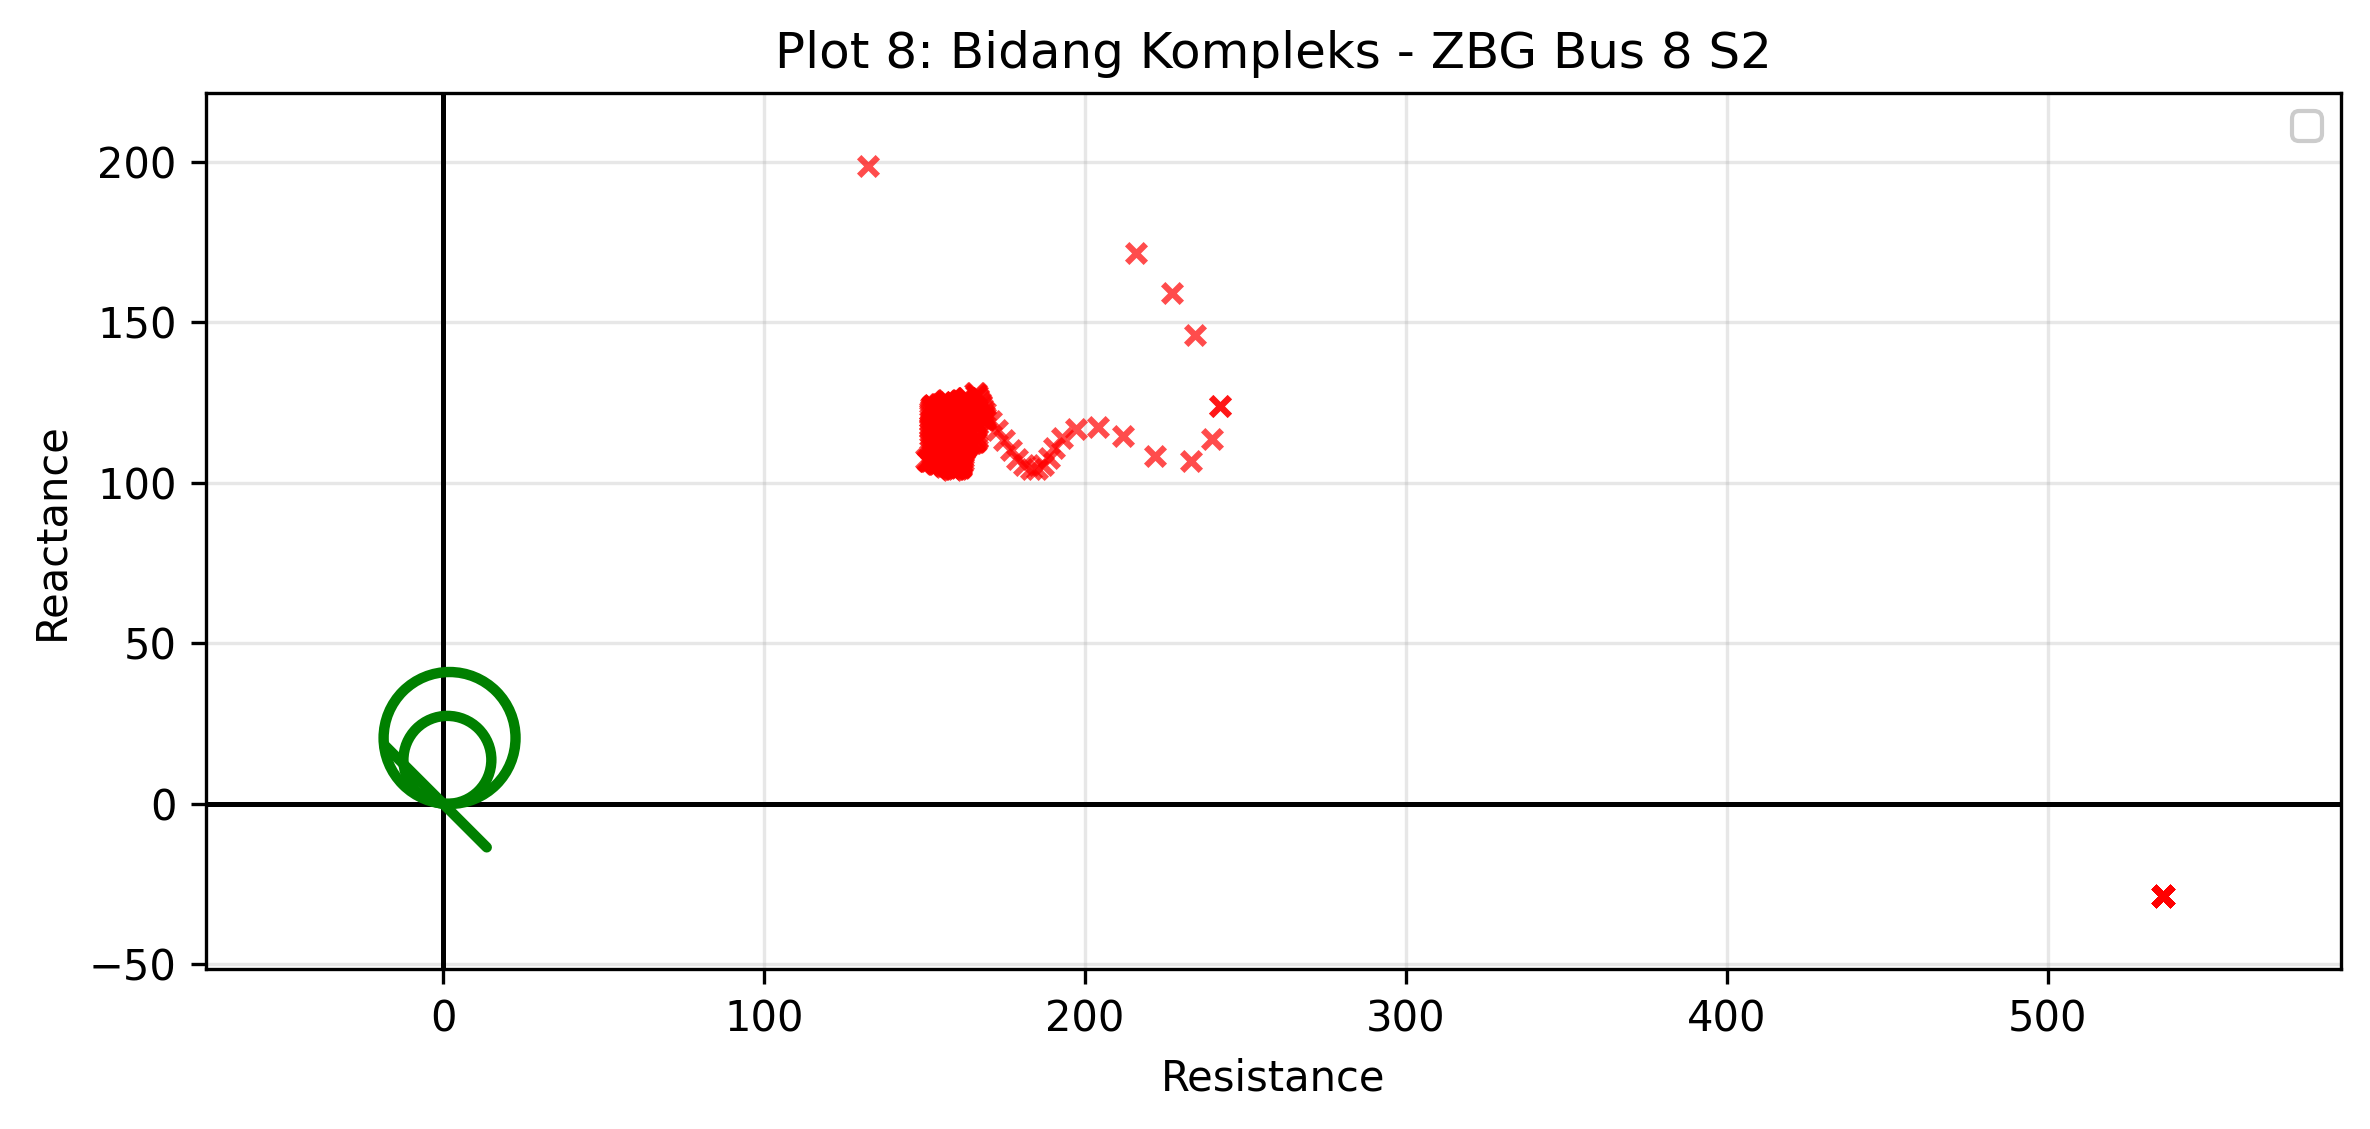
\includegraphics[width=0.8\textwidth]{contents/chapter-4/PRIA_08_ZBG_Bus_8_S2.png}
%     \caption{Impedansi Tampak ZBG Bus 8 Skenario 2}
%     \label{fig:PRIA_08_ZBG_Bus_8_S2}
% \end{figure}

% \begin{figure}[H]
%     \centering
%     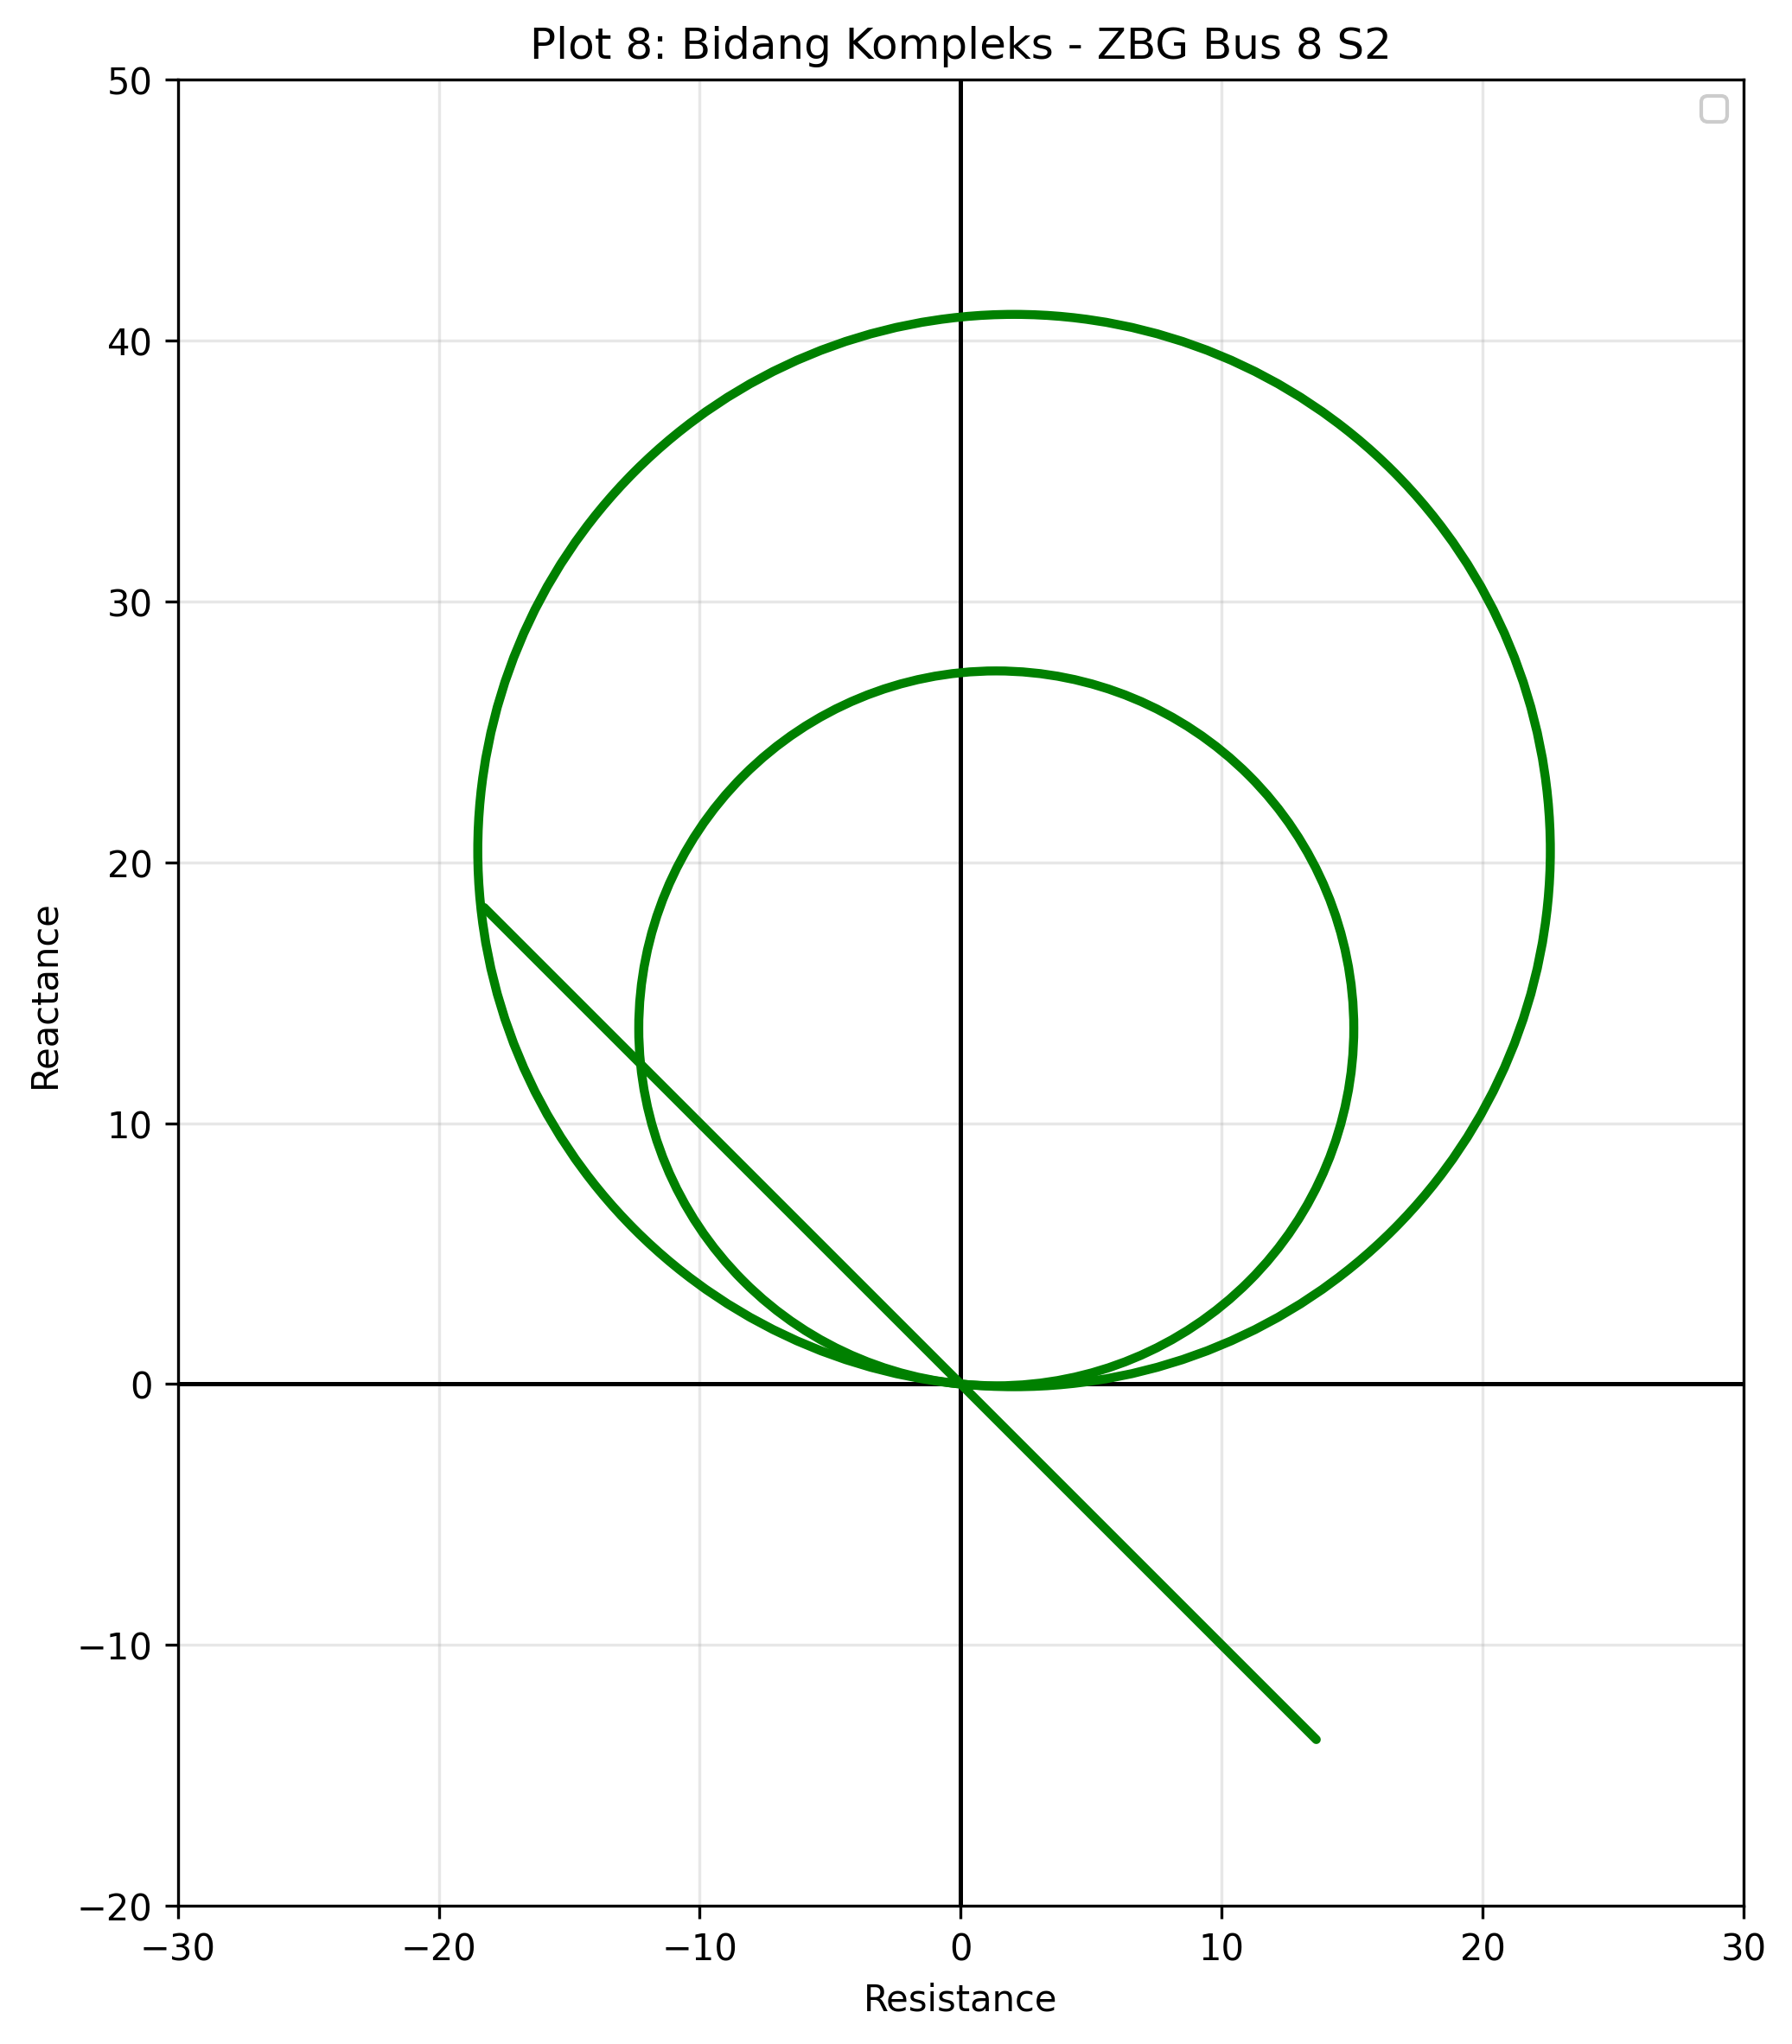
\includegraphics[width=0.8\textwidth]{contents/chapter-4/PRIZI_08_ZBG_Bus_8_S2.png}
%     \caption{Impedansi Tampak ZBG Bus 8 Skenario 2}
%     \label{fig:PRIZI_08_ZBG_Bus_8_S2}
% \end{figure}

\begin{figure}[H]
    \centering

    % Gambar sebelah kiri
    \begin{subfigure}[t]{0.48\textwidth}
        \centering
        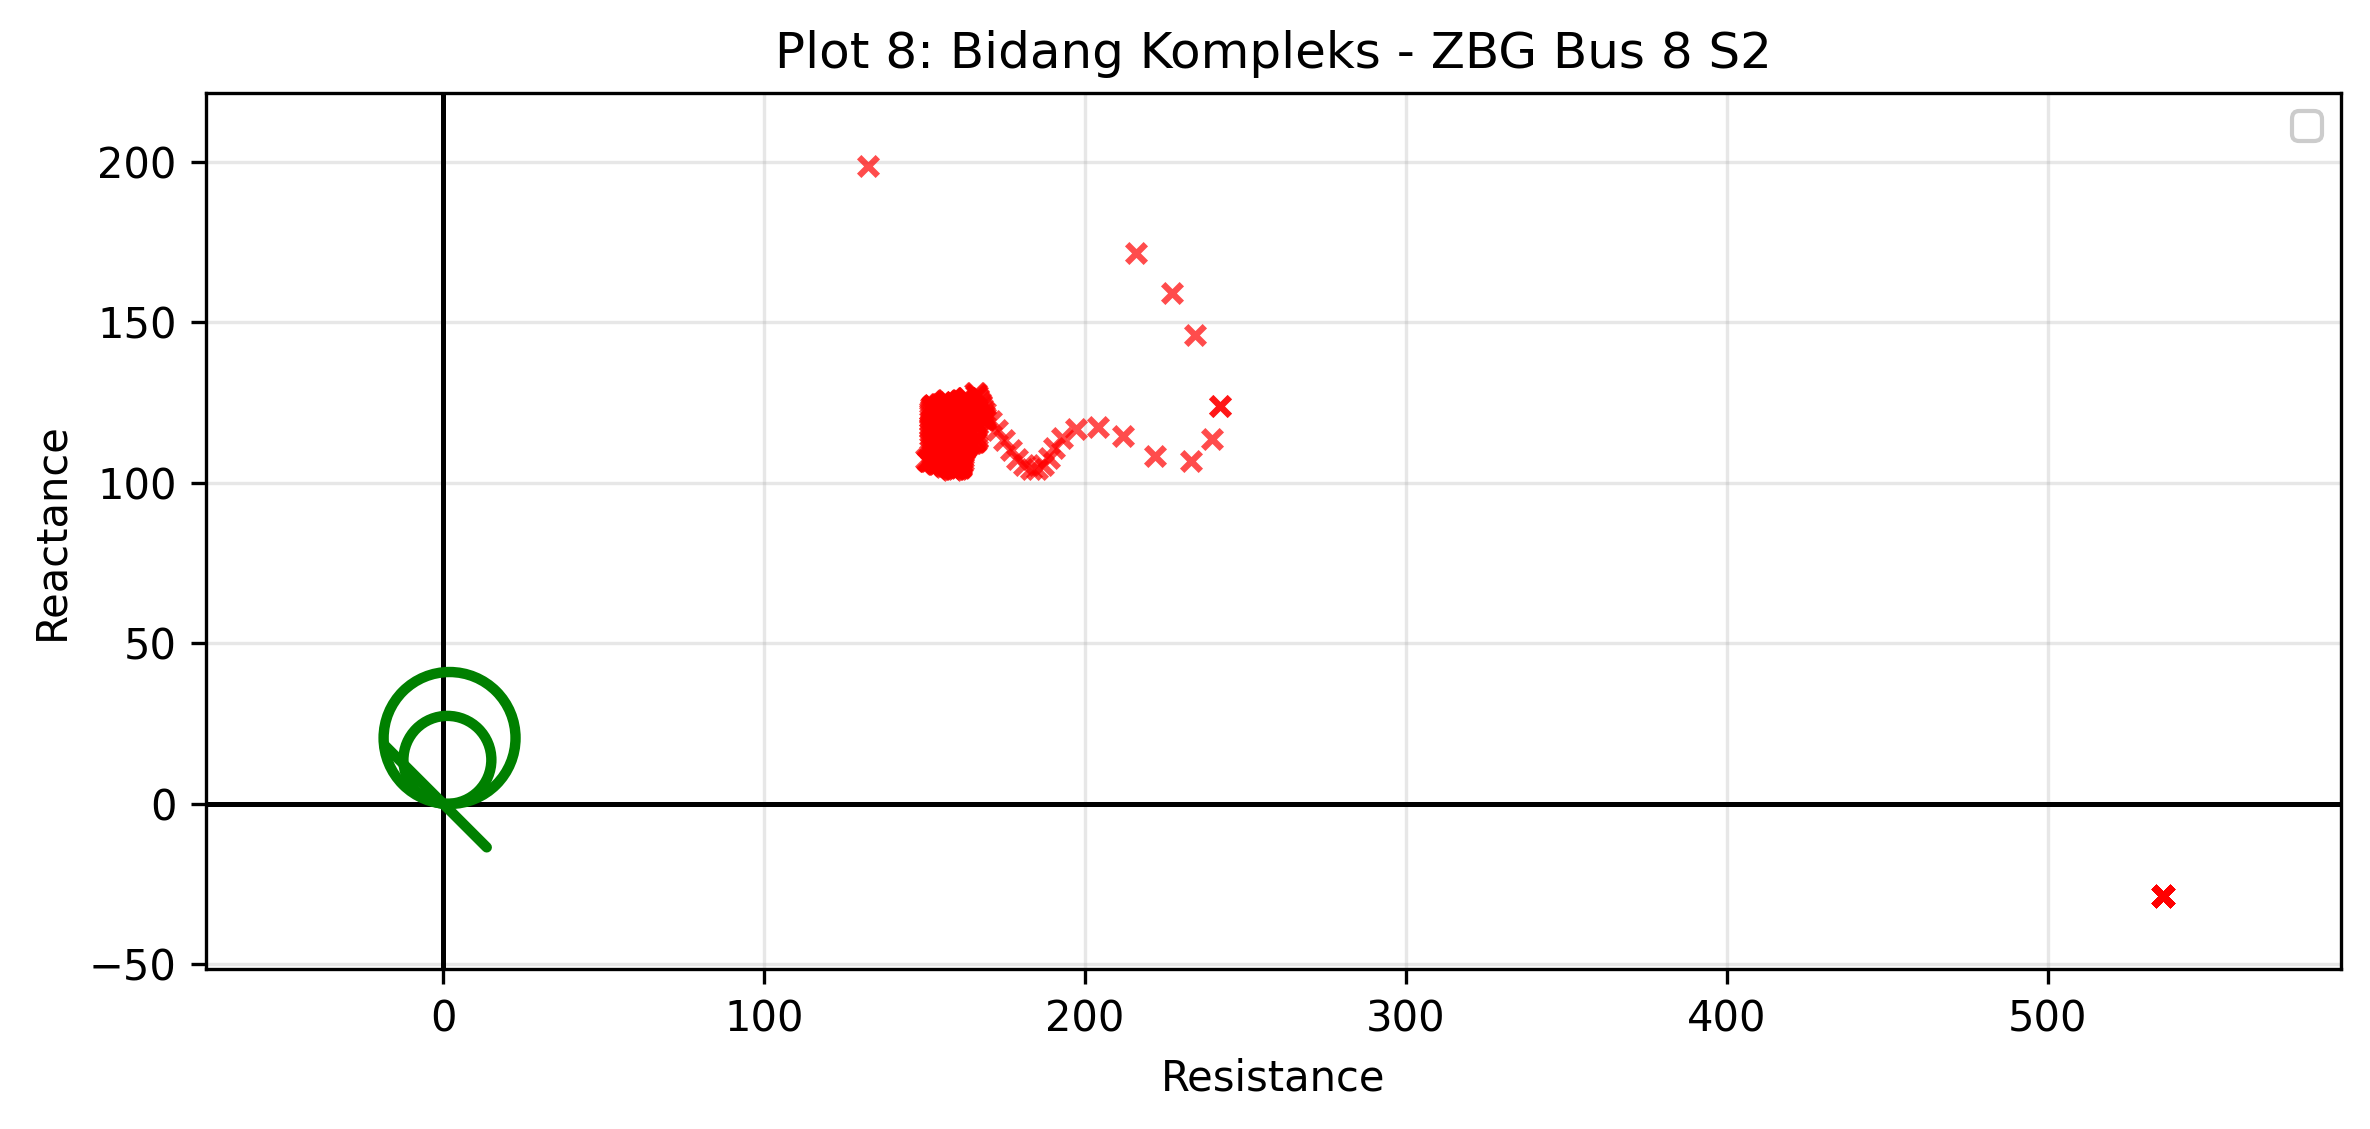
\includegraphics[width=\textwidth]{contents/chapter-4/PRIA_08_ZBG_Bus_8_S2.png}
        \caption{Seluruh Impedansi Tampak}
        \label{fig:PRIA_08_ZBG_Bus_8_S2}
    \end{subfigure}
    \hfill
    % Gambar sebelah kanan
    \begin{subfigure}[t]{0.48\textwidth}
        \centering
        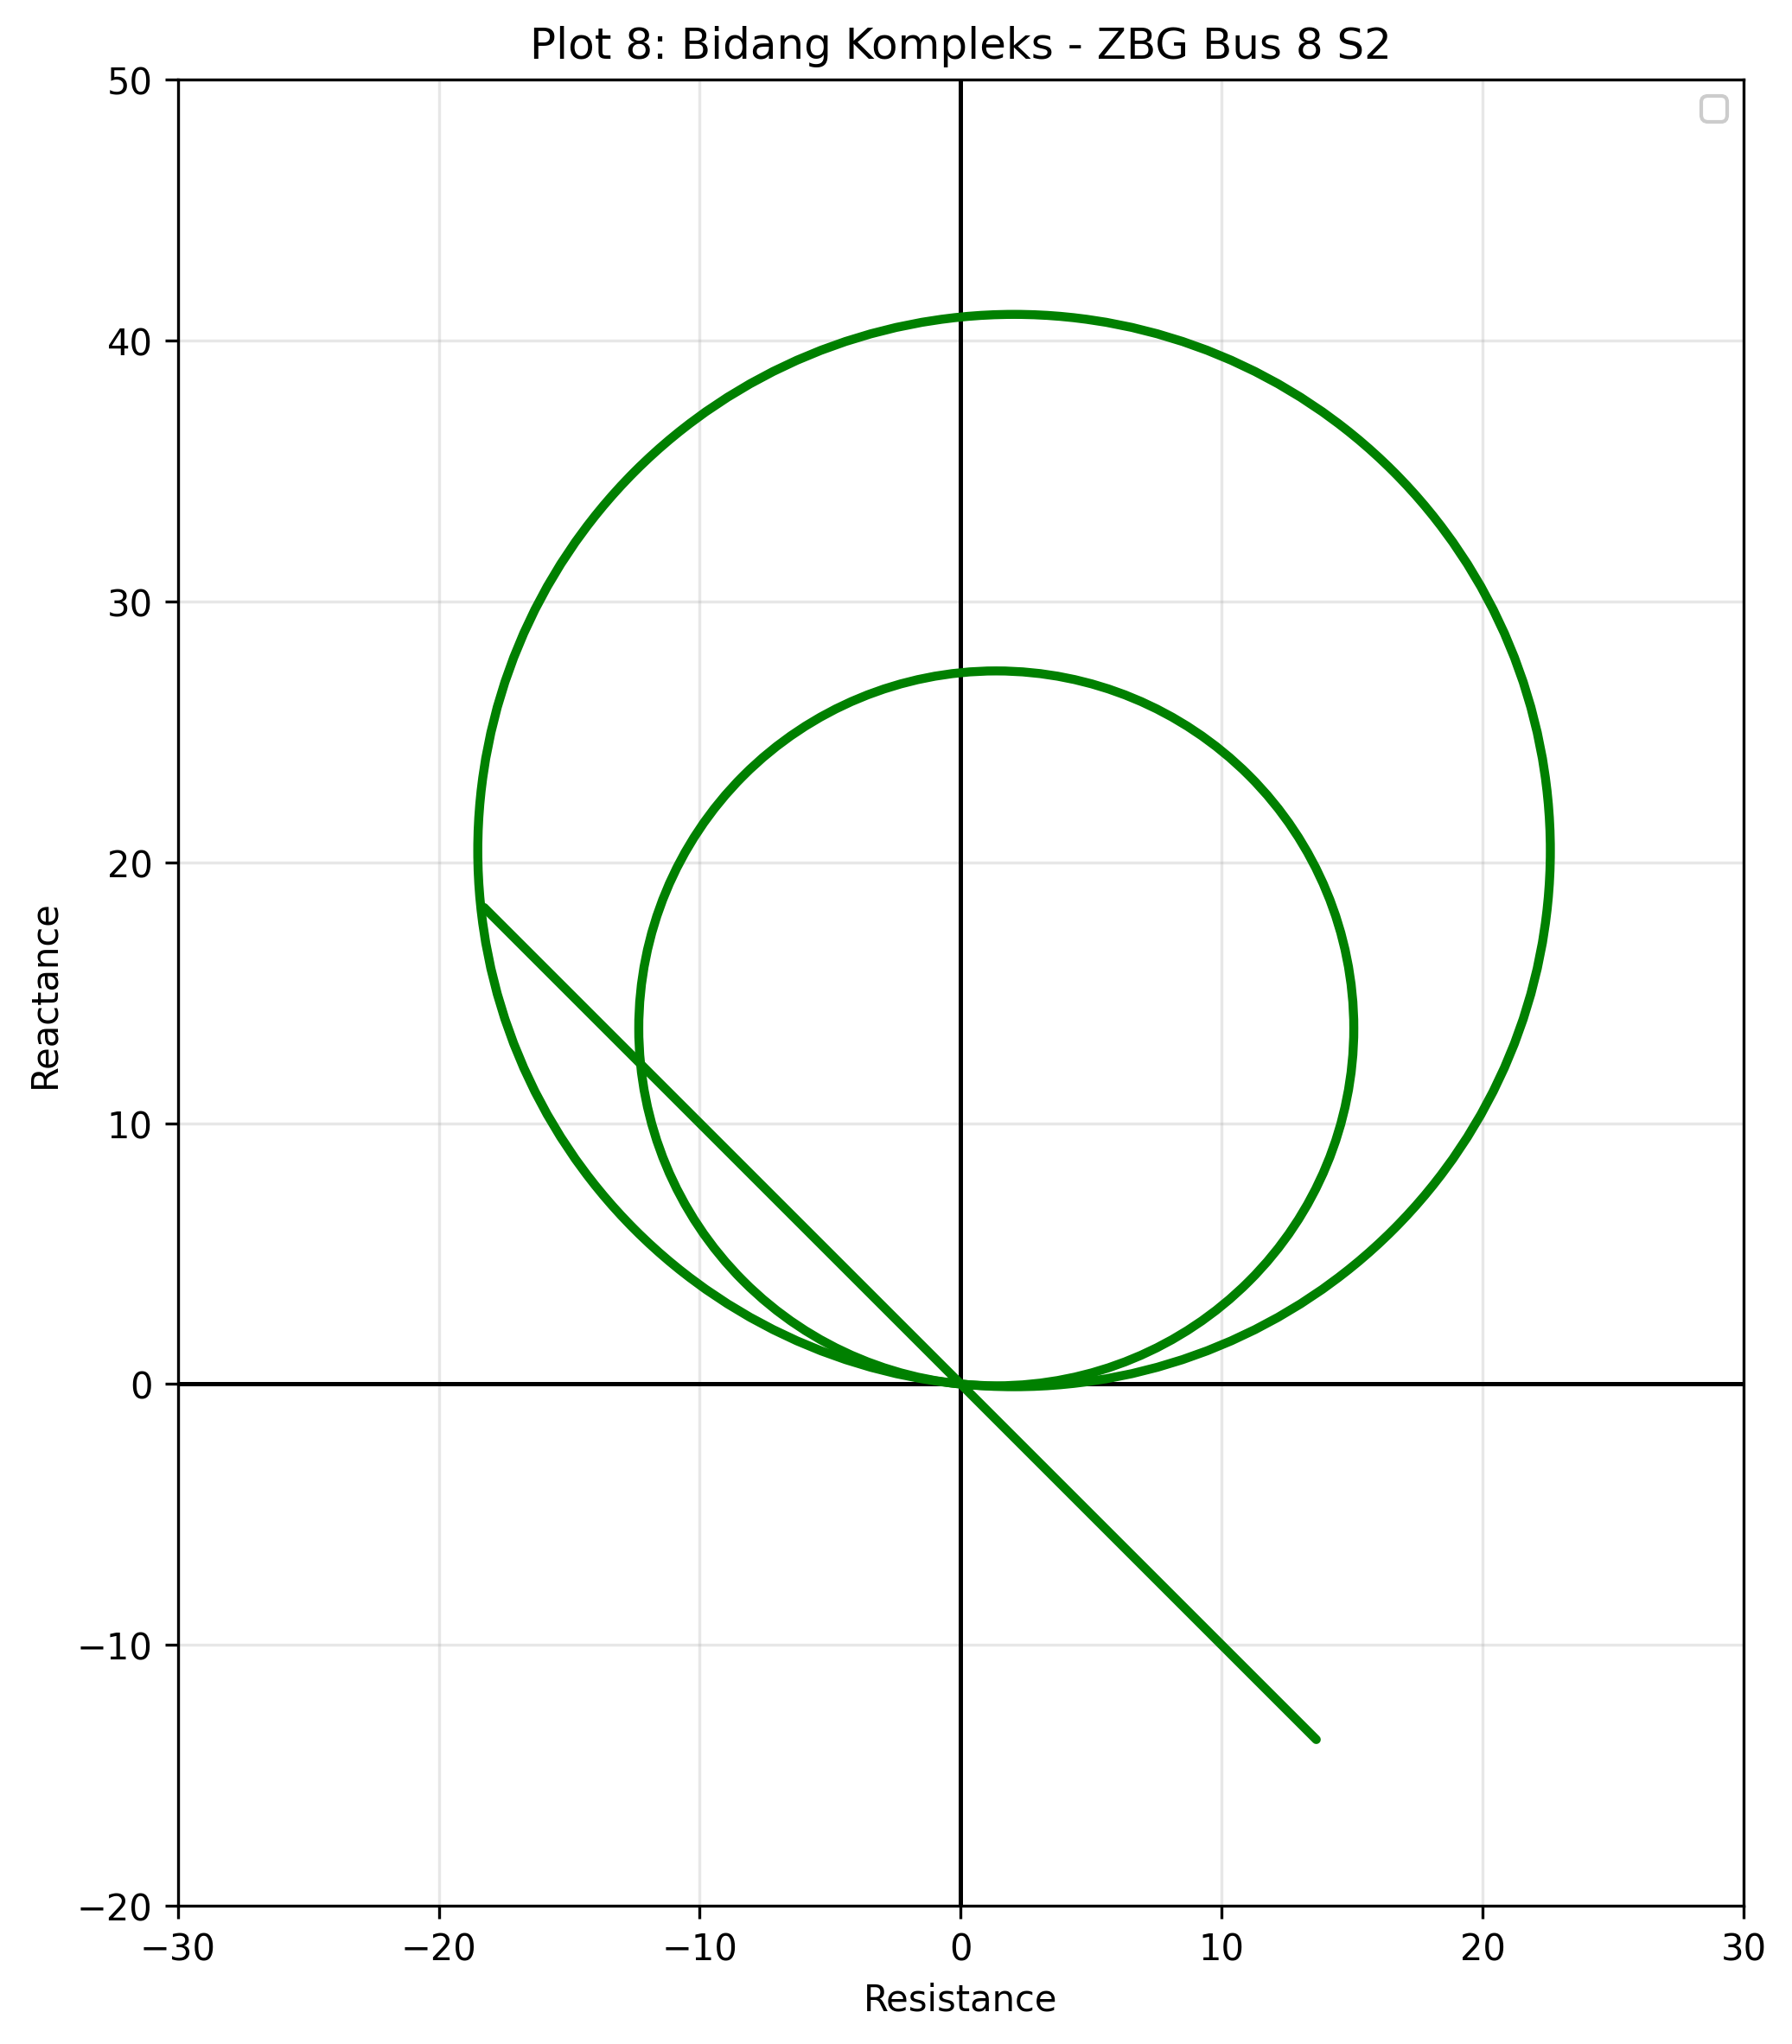
\includegraphics[width=\textwidth]{contents/chapter-4/PRIZI_08_ZBG_Bus_8_S2.png}
        \caption{Zoom In Pada Zona Proteksi}
        \label{fig:PRIZI_08_ZBG_Bus_8_S2}
    \end{subfigure}

    \caption{Impedansi Tampak ZBG Bus 8 Skenario 2}
    \label{fig:Impedansi_Tampak_ZBG_Bus_8_S2}
\end{figure}

Gambar \ref{fig:Impedansi_Tampak_ZBG_Bus_8_S2} menunjukkan bahwa impedansi tampak loop fasa B dengan ground yang dibaca oleh relay 21 sisi Bus 8 juga tidak masuk ke dalam zona proteksi. Hasil tersebut masih konsisten dengan arus sekunder CT pada Gambar \ref{fig:Bus_8_Ex_DLG_S2}, yaitu arus gangguan belum memenuhi syarat \textit{starting} untuk membuat relay aktif. Oleh karena itu, jika dibandingkan dengan acuan gangguan eksternal DLG pada Subbab \ref{subsec:tanpa_IBR_ex_dlg}, respons relay 21 sisi Bus 8 pada elemen ini juga menunjukkan \textit{misoperation}.

%%%%%%%%%%%%%%%%%%%%%%%%%%%%%%%%%%%%%%%%%%%%%%%%%%%%%%%%%%%%%%

% \begin{figure}[H]
%     \centering
%     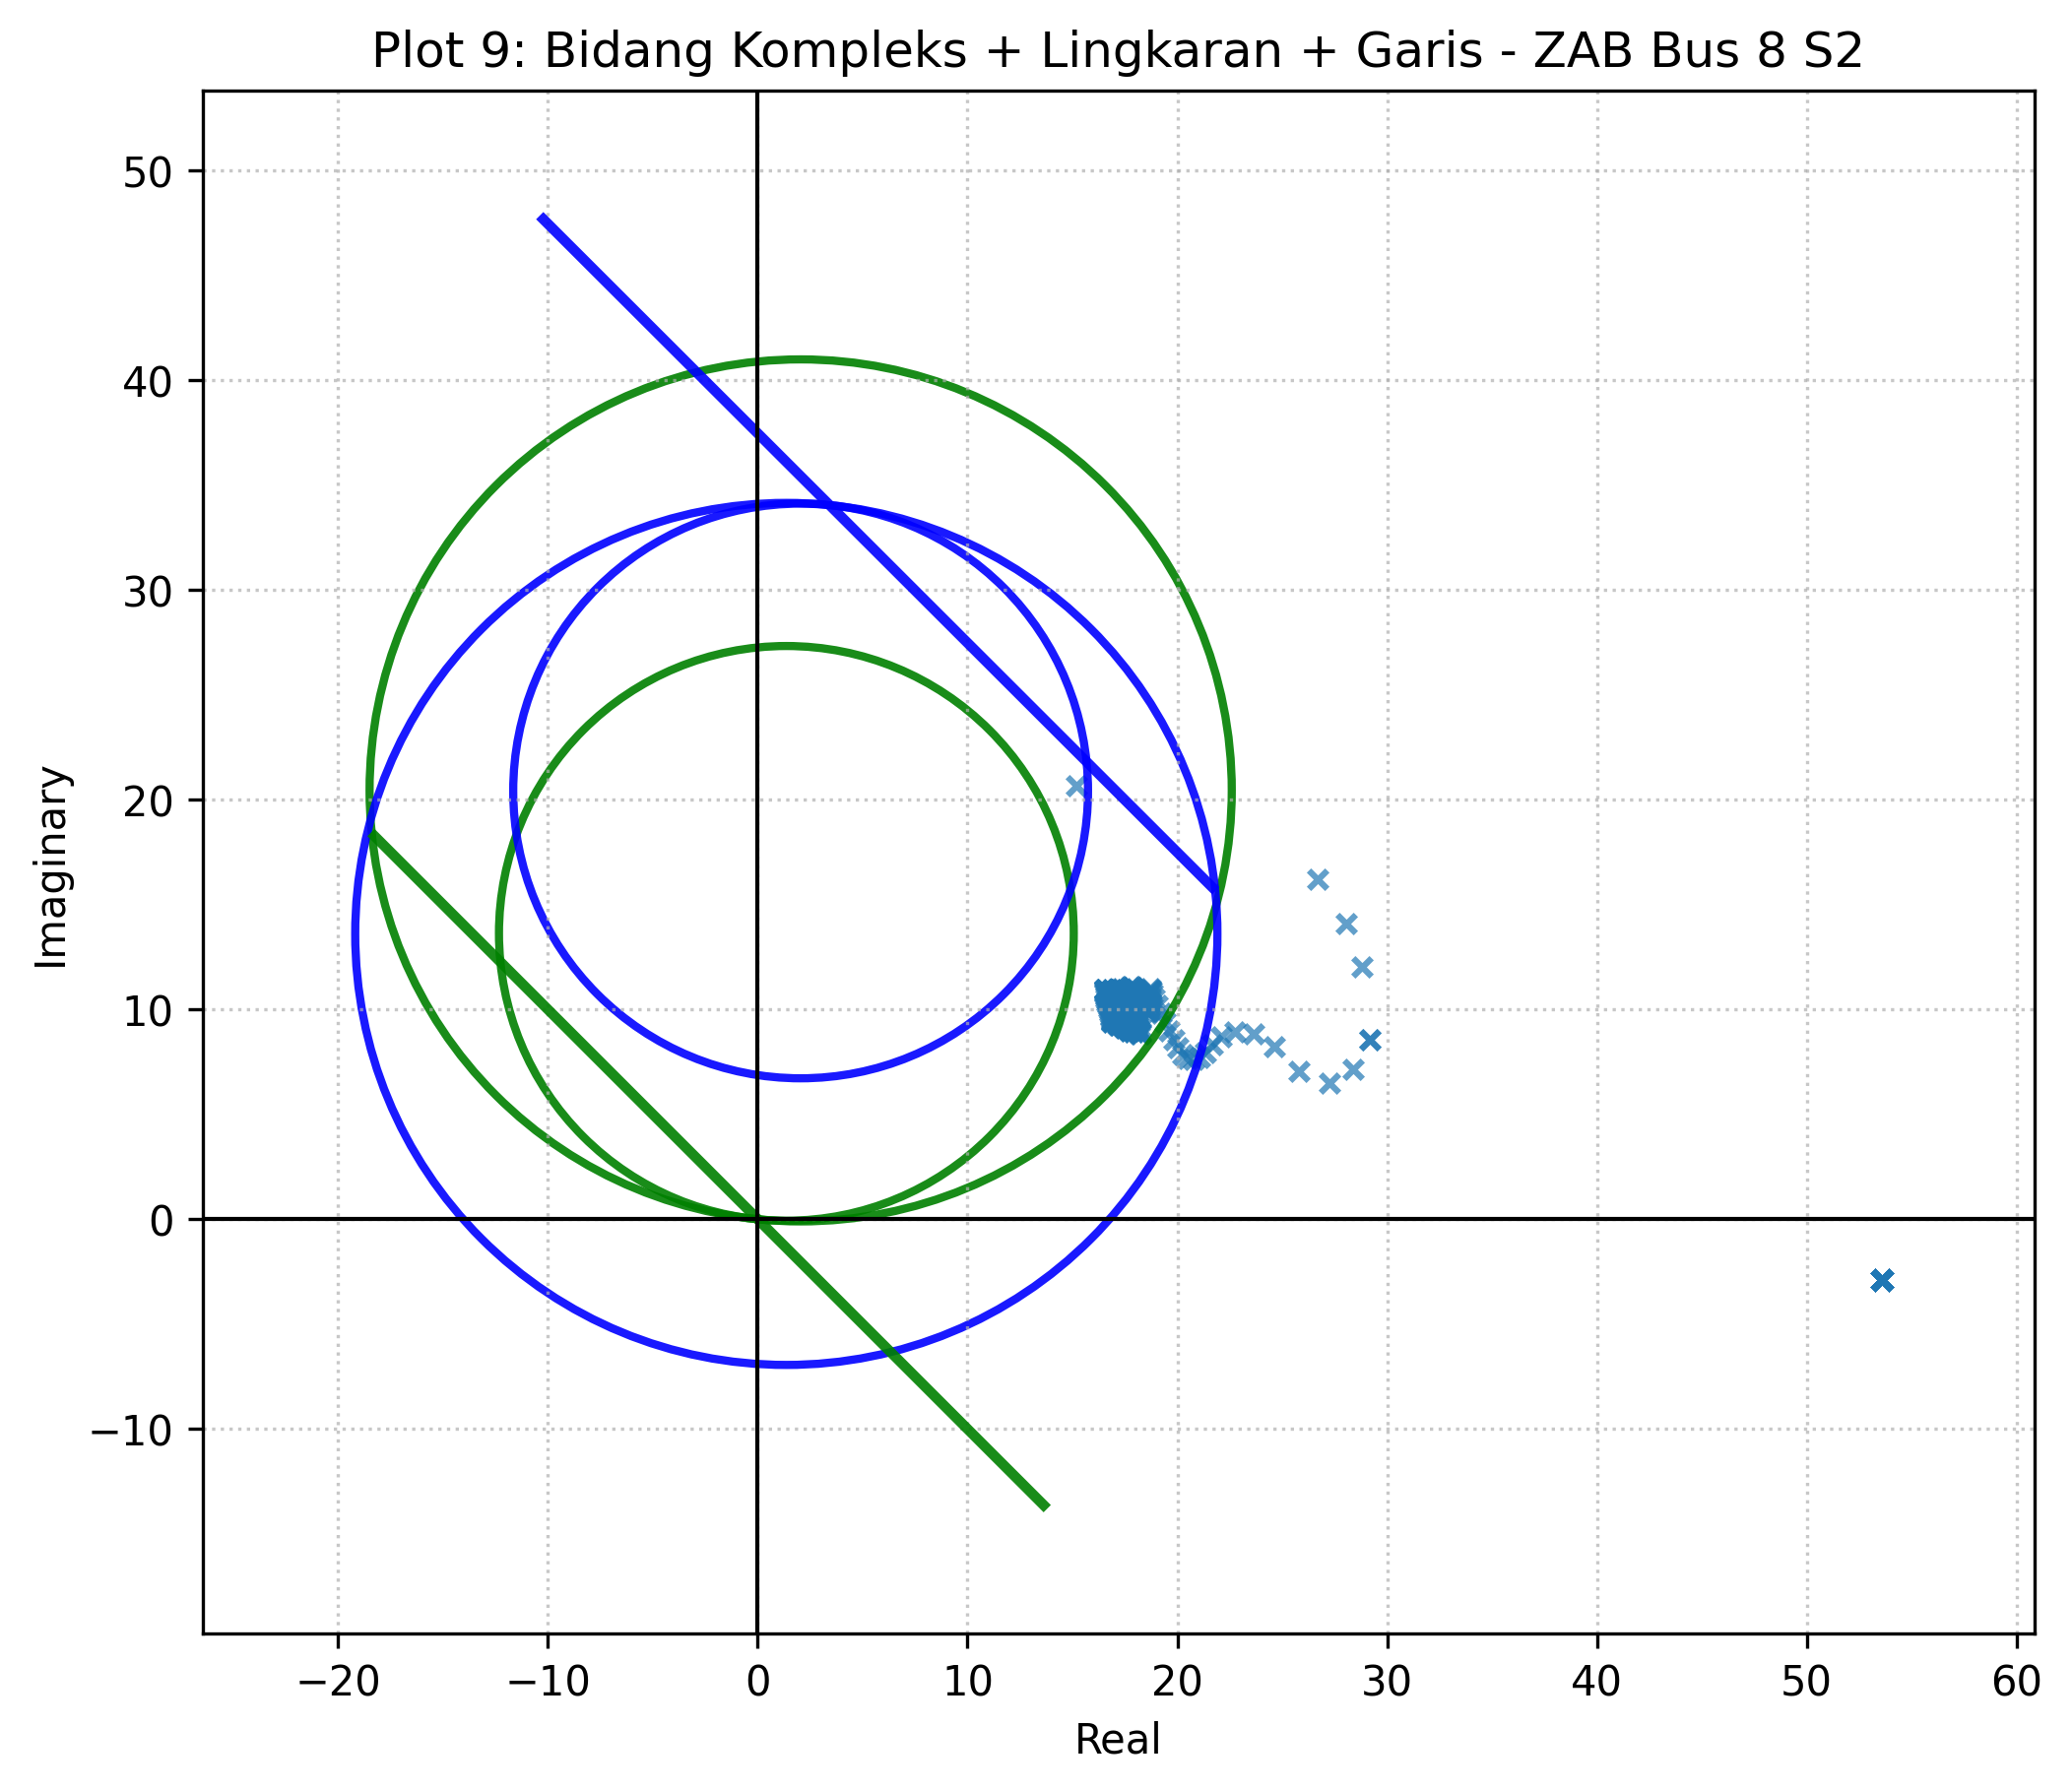
\includegraphics[width=0.8\textwidth]{contents/chapter-4/09_ZAB_Bus_8_S2_dengan_lingkaran_dan_garis.png}
%     \caption{Impedansi Tampak ZAB Bus 8 Skenario 2}
%     \label{fig:09_ZAB_Bus_8_S2_dengan_lingkaran_dan_garis}
% \end{figure}

% untuk gambar \ref{fig:09_ZAB_Bus_8_S2_dengan_lingkaran_dan_garis} masih sama dengan dengan gambar \ref{fig:07_ZAG_Bus_8_S2_dengan_lingkaran_dan_garis} dan \ref{fig:08_ZBG_Bus_8_S2_dengan_lingkaran_dan_garis} dimana terlihat untuk titik impedansi tampak ZAB terlihat cukup bergerak dan relay 21 dari sisi bus 8 mengalami over reach pada zona 1 yang seharusnya masuk pada zona 2. pada sisi ini, relay juga mengalami dropout zona 2 yang seharusnya masih dalam jangkauannya.

% Terlihat pada gambar \ref{fig:09_ZAB_Bus_8_S2_dengan_lingkaran_dan_garis} bahwa impedansi tampak pada fasa A dengan fasa B yang dibaca oleh relay 21 sisi bus 8 saat terdapat gangguan external DLG bekerja dengan acuan pada \ref{subsec:tanpa_IBR_in_dlg} relay 21 bus 8 mengalami misoperation karena mendeteksi adanya gangguan namun overreach pada zona 1 yang seharusnya pada zona 2 serta mengalami dropout pada zona 2 dan memberikan sinyal trip kepada CB pada zona 2

%%%%%%%%%%%%%%%%%%%%%%%%%%%%%%%%%SISI PRIMER%%%%%%%%%%%%%%%%%%%%%%%%%%%%%%%%%%

% \begin{figure}[H]
%     \centering
%     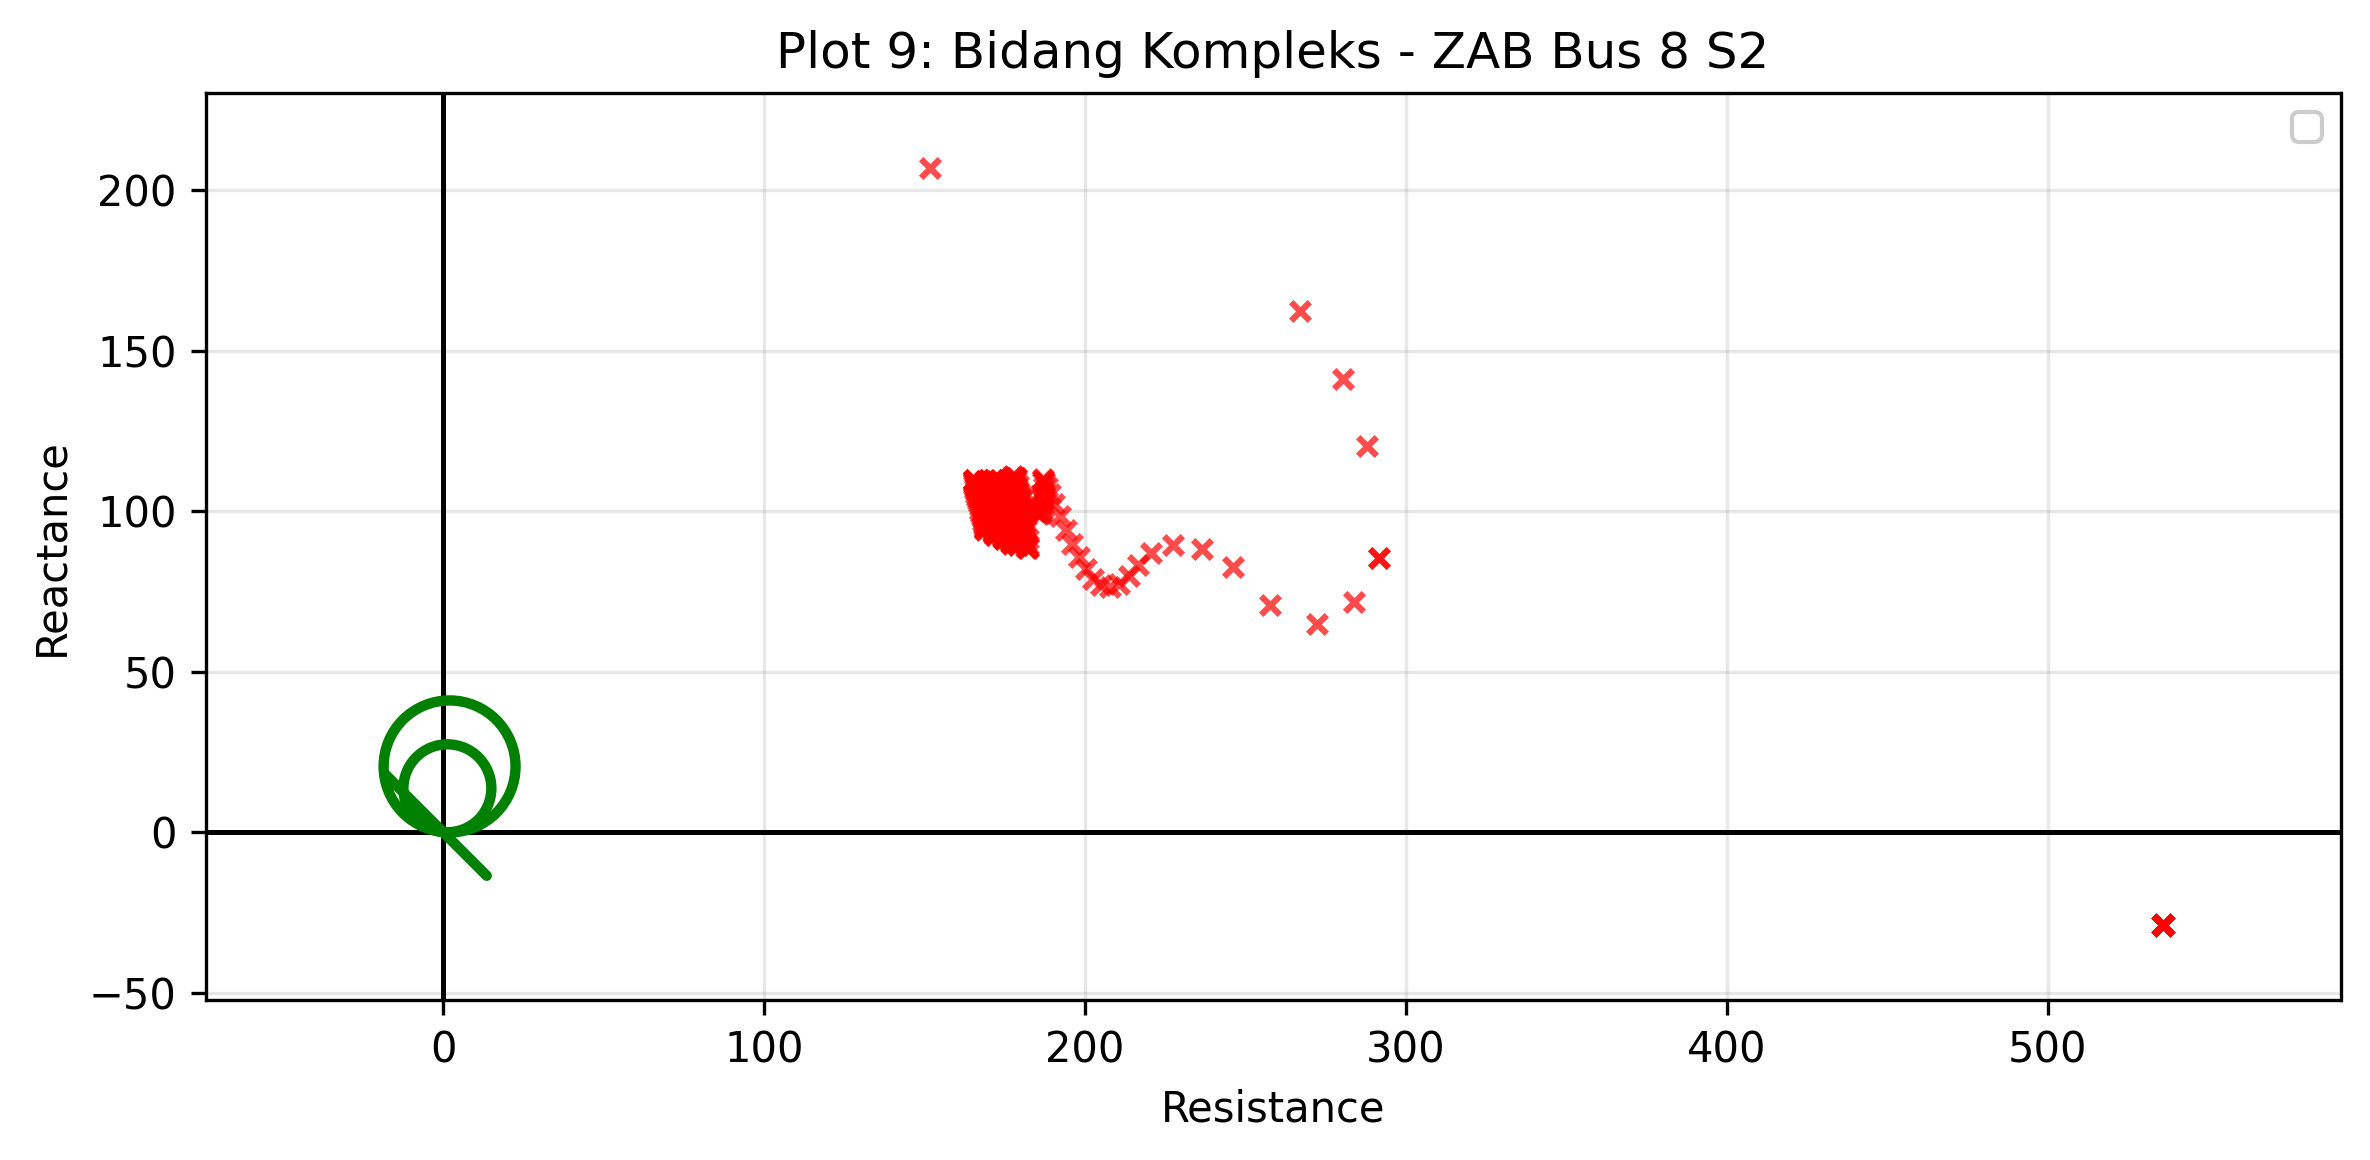
\includegraphics[width=0.8\textwidth]{contents/chapter-4/PRIA_09_ZAB_Bus_8_S2.png}
%     \caption{Impedansi Tampak ZAB Bus 8 Skenario 2}
%     \label{fig:PRIA_09_ZAB_Bus_8_S2}
% \end{figure}

% \begin{figure}[H]
%     \centering
%     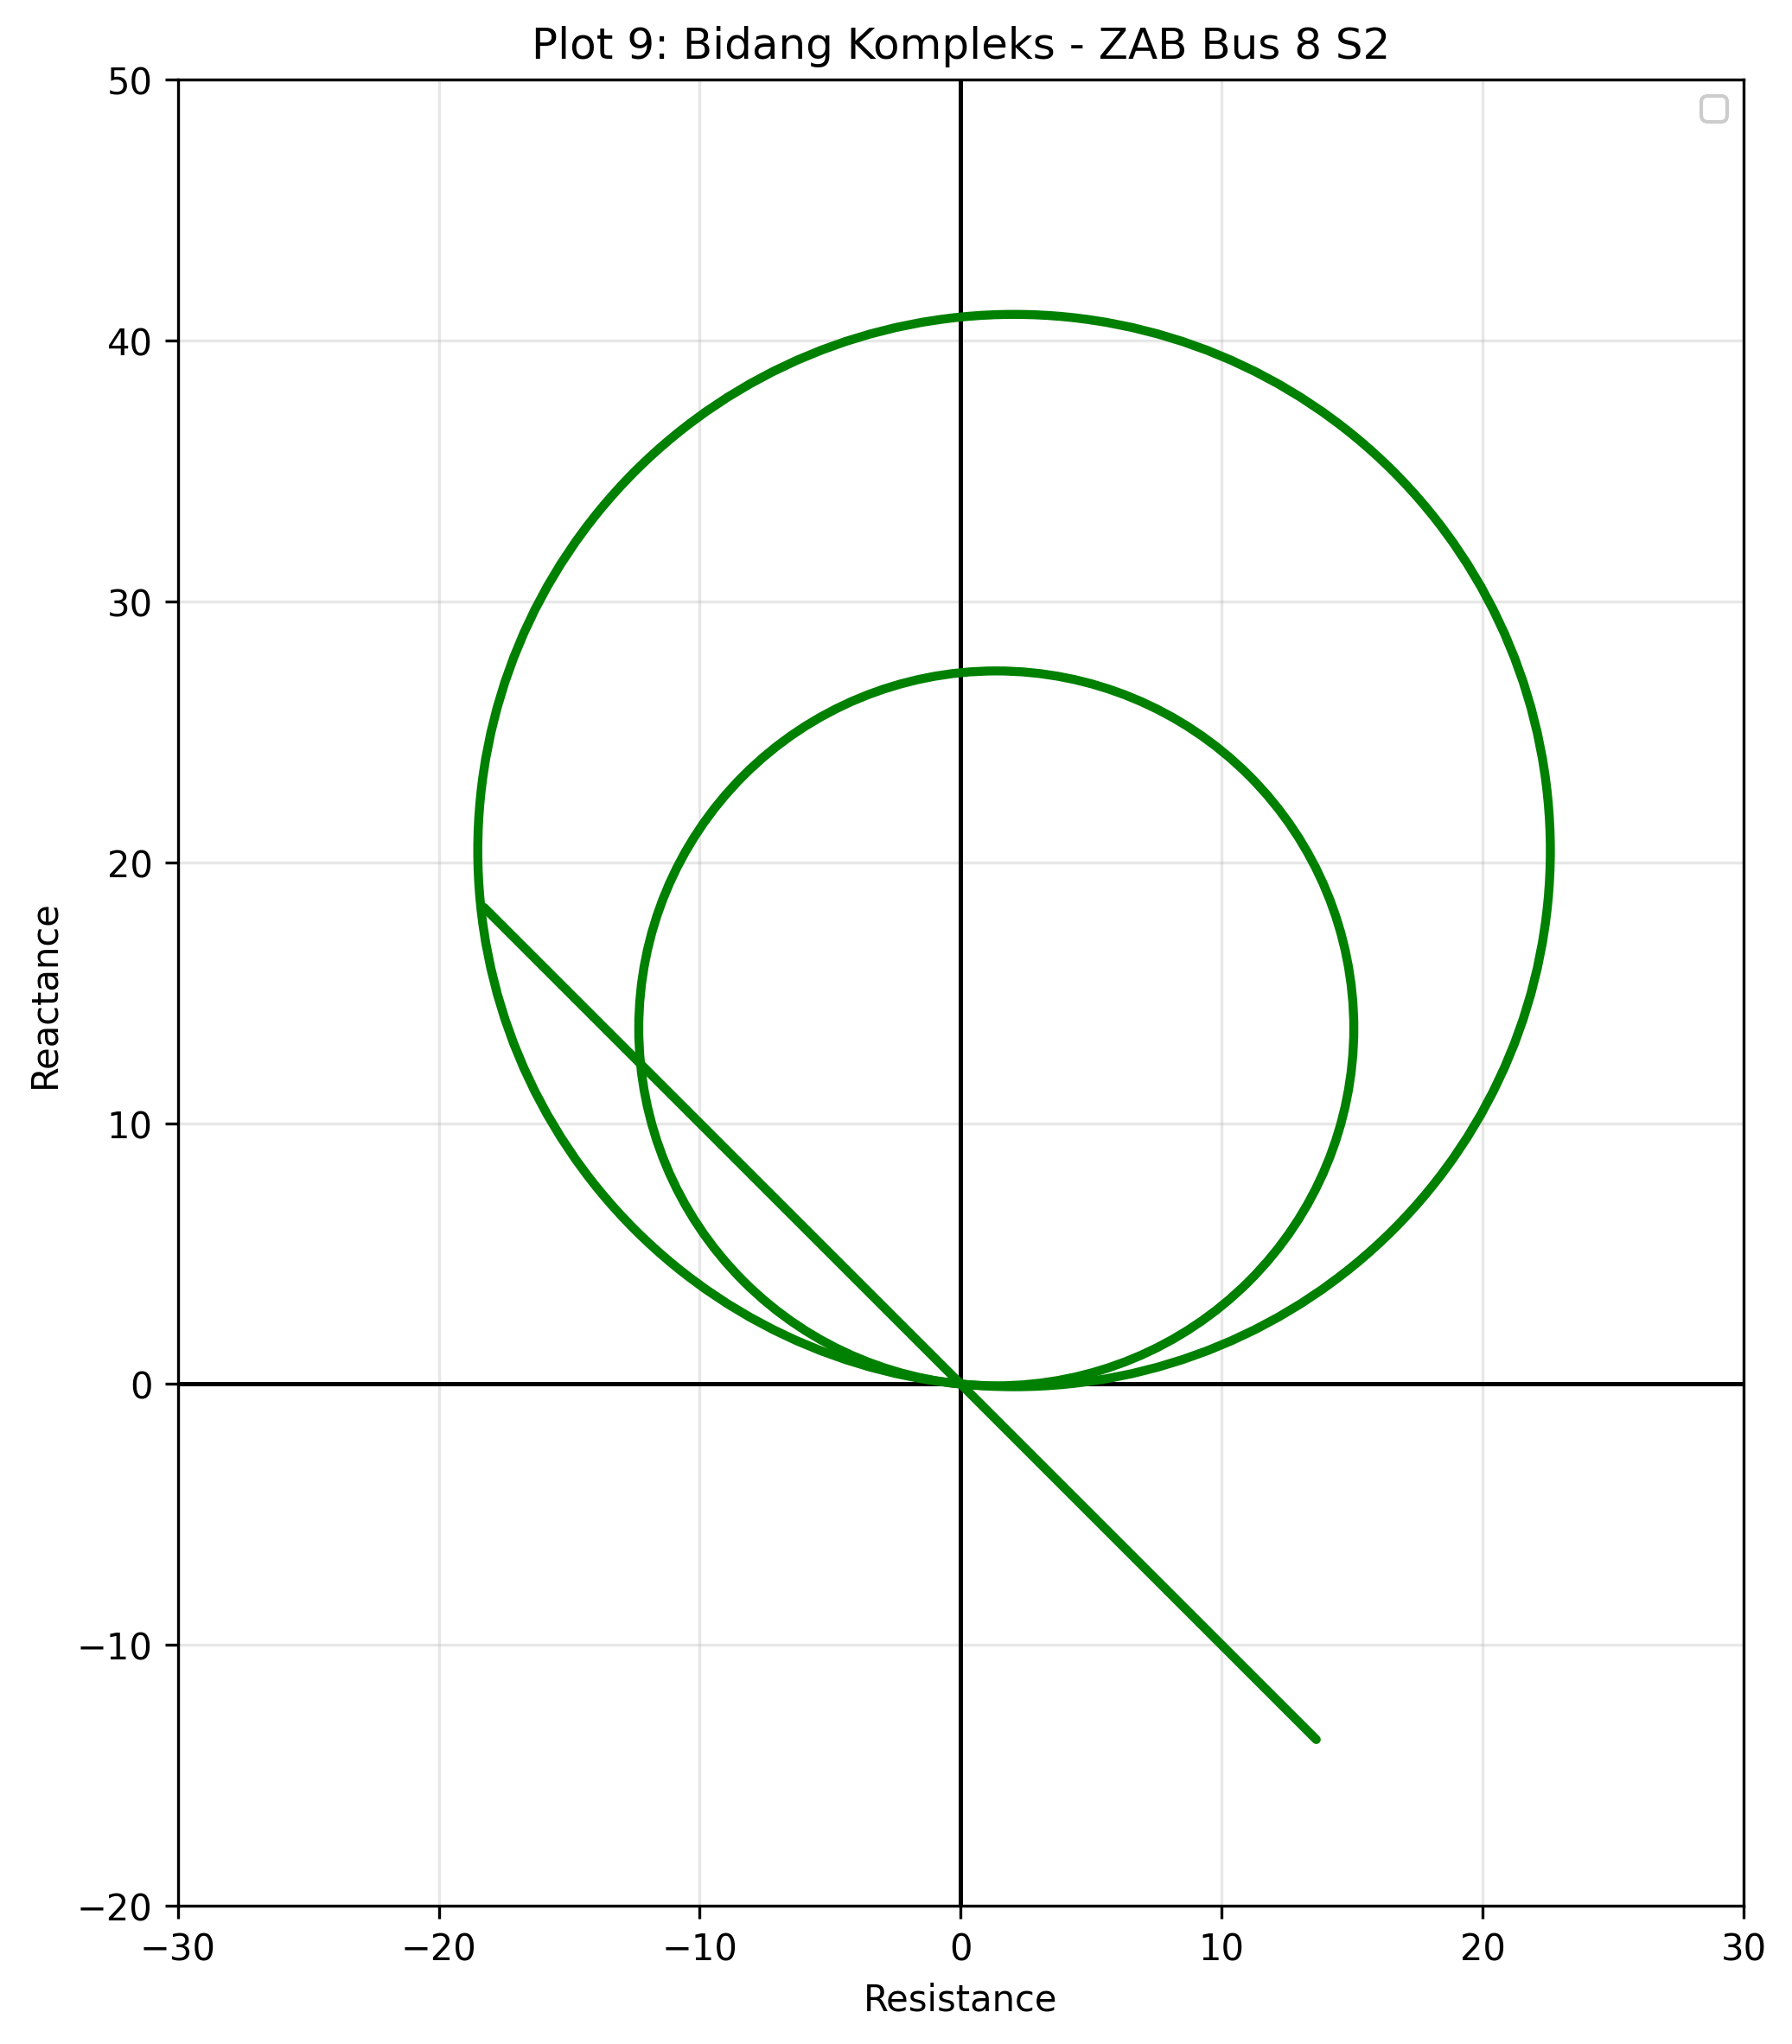
\includegraphics[width=0.8\textwidth]{contents/chapter-4/PRIZI_09_ZAB_Bus_8_S2.png}
%     \caption{Impedansi Tampak ZAB Bus 8 Skenario 2}
%     \label{fig:PRIZI_09_ZAB_Bus_8_S2}
% \end{figure}

\begin{figure}[H]
    \centering

    % Gambar sebelah kiri
    \begin{subfigure}[t]{0.48\textwidth}
        \centering
        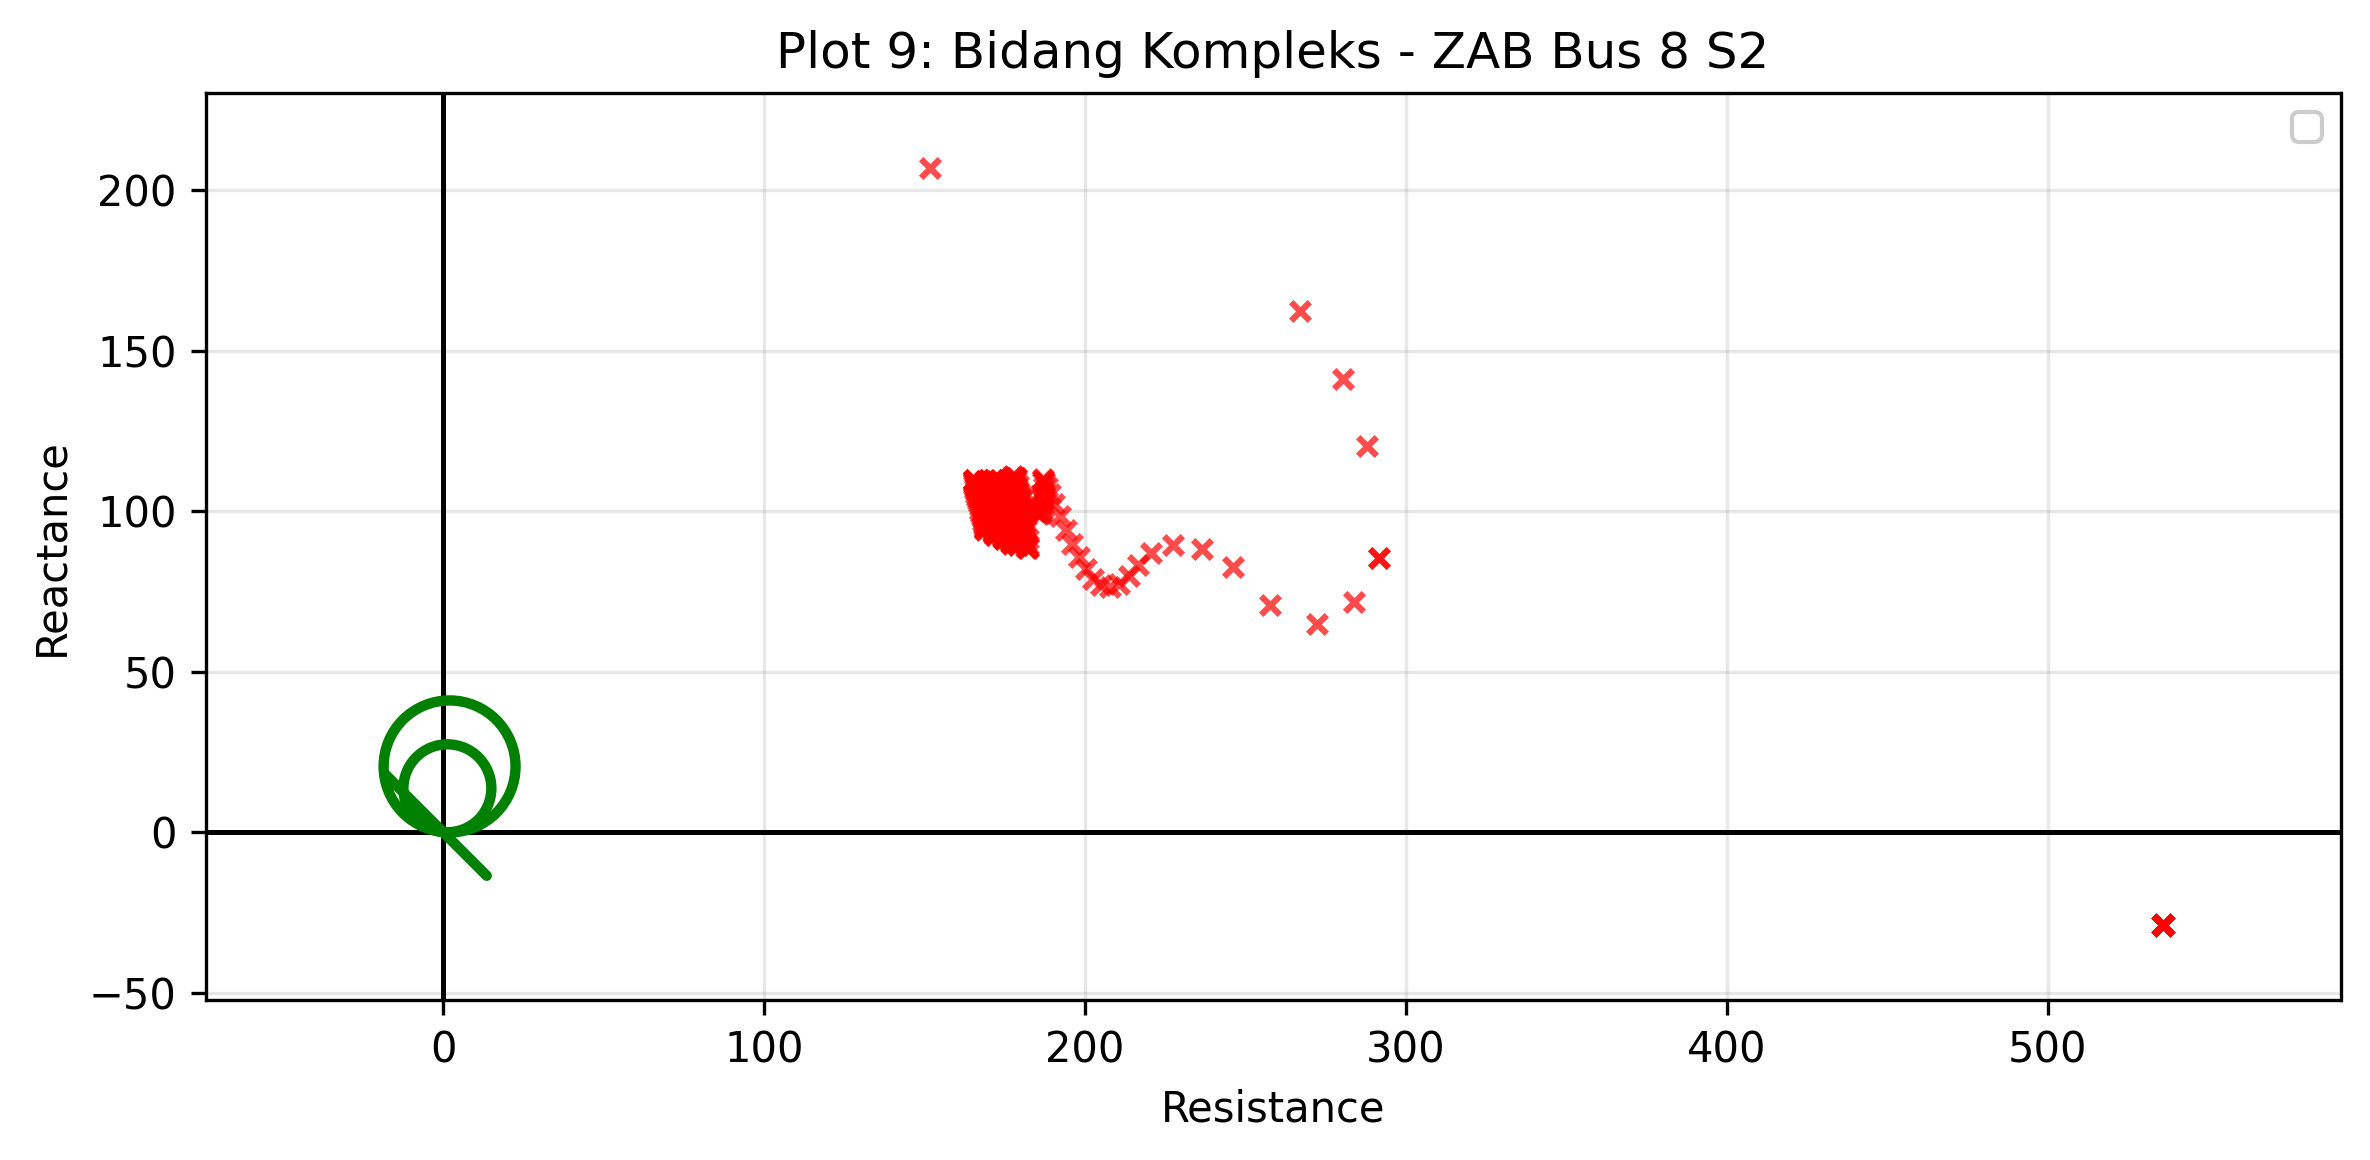
\includegraphics[width=\textwidth]{contents/chapter-4/PRIA_09_ZAB_Bus_8_S2.png}
        \caption{Seluruh Impedansi Tampak}
        \label{fig:PRIA_09_ZAB_Bus_8_S2}
    \end{subfigure}
    \hfill
    % Gambar sebelah kanan
    \begin{subfigure}[t]{0.48\textwidth}
        \centering
        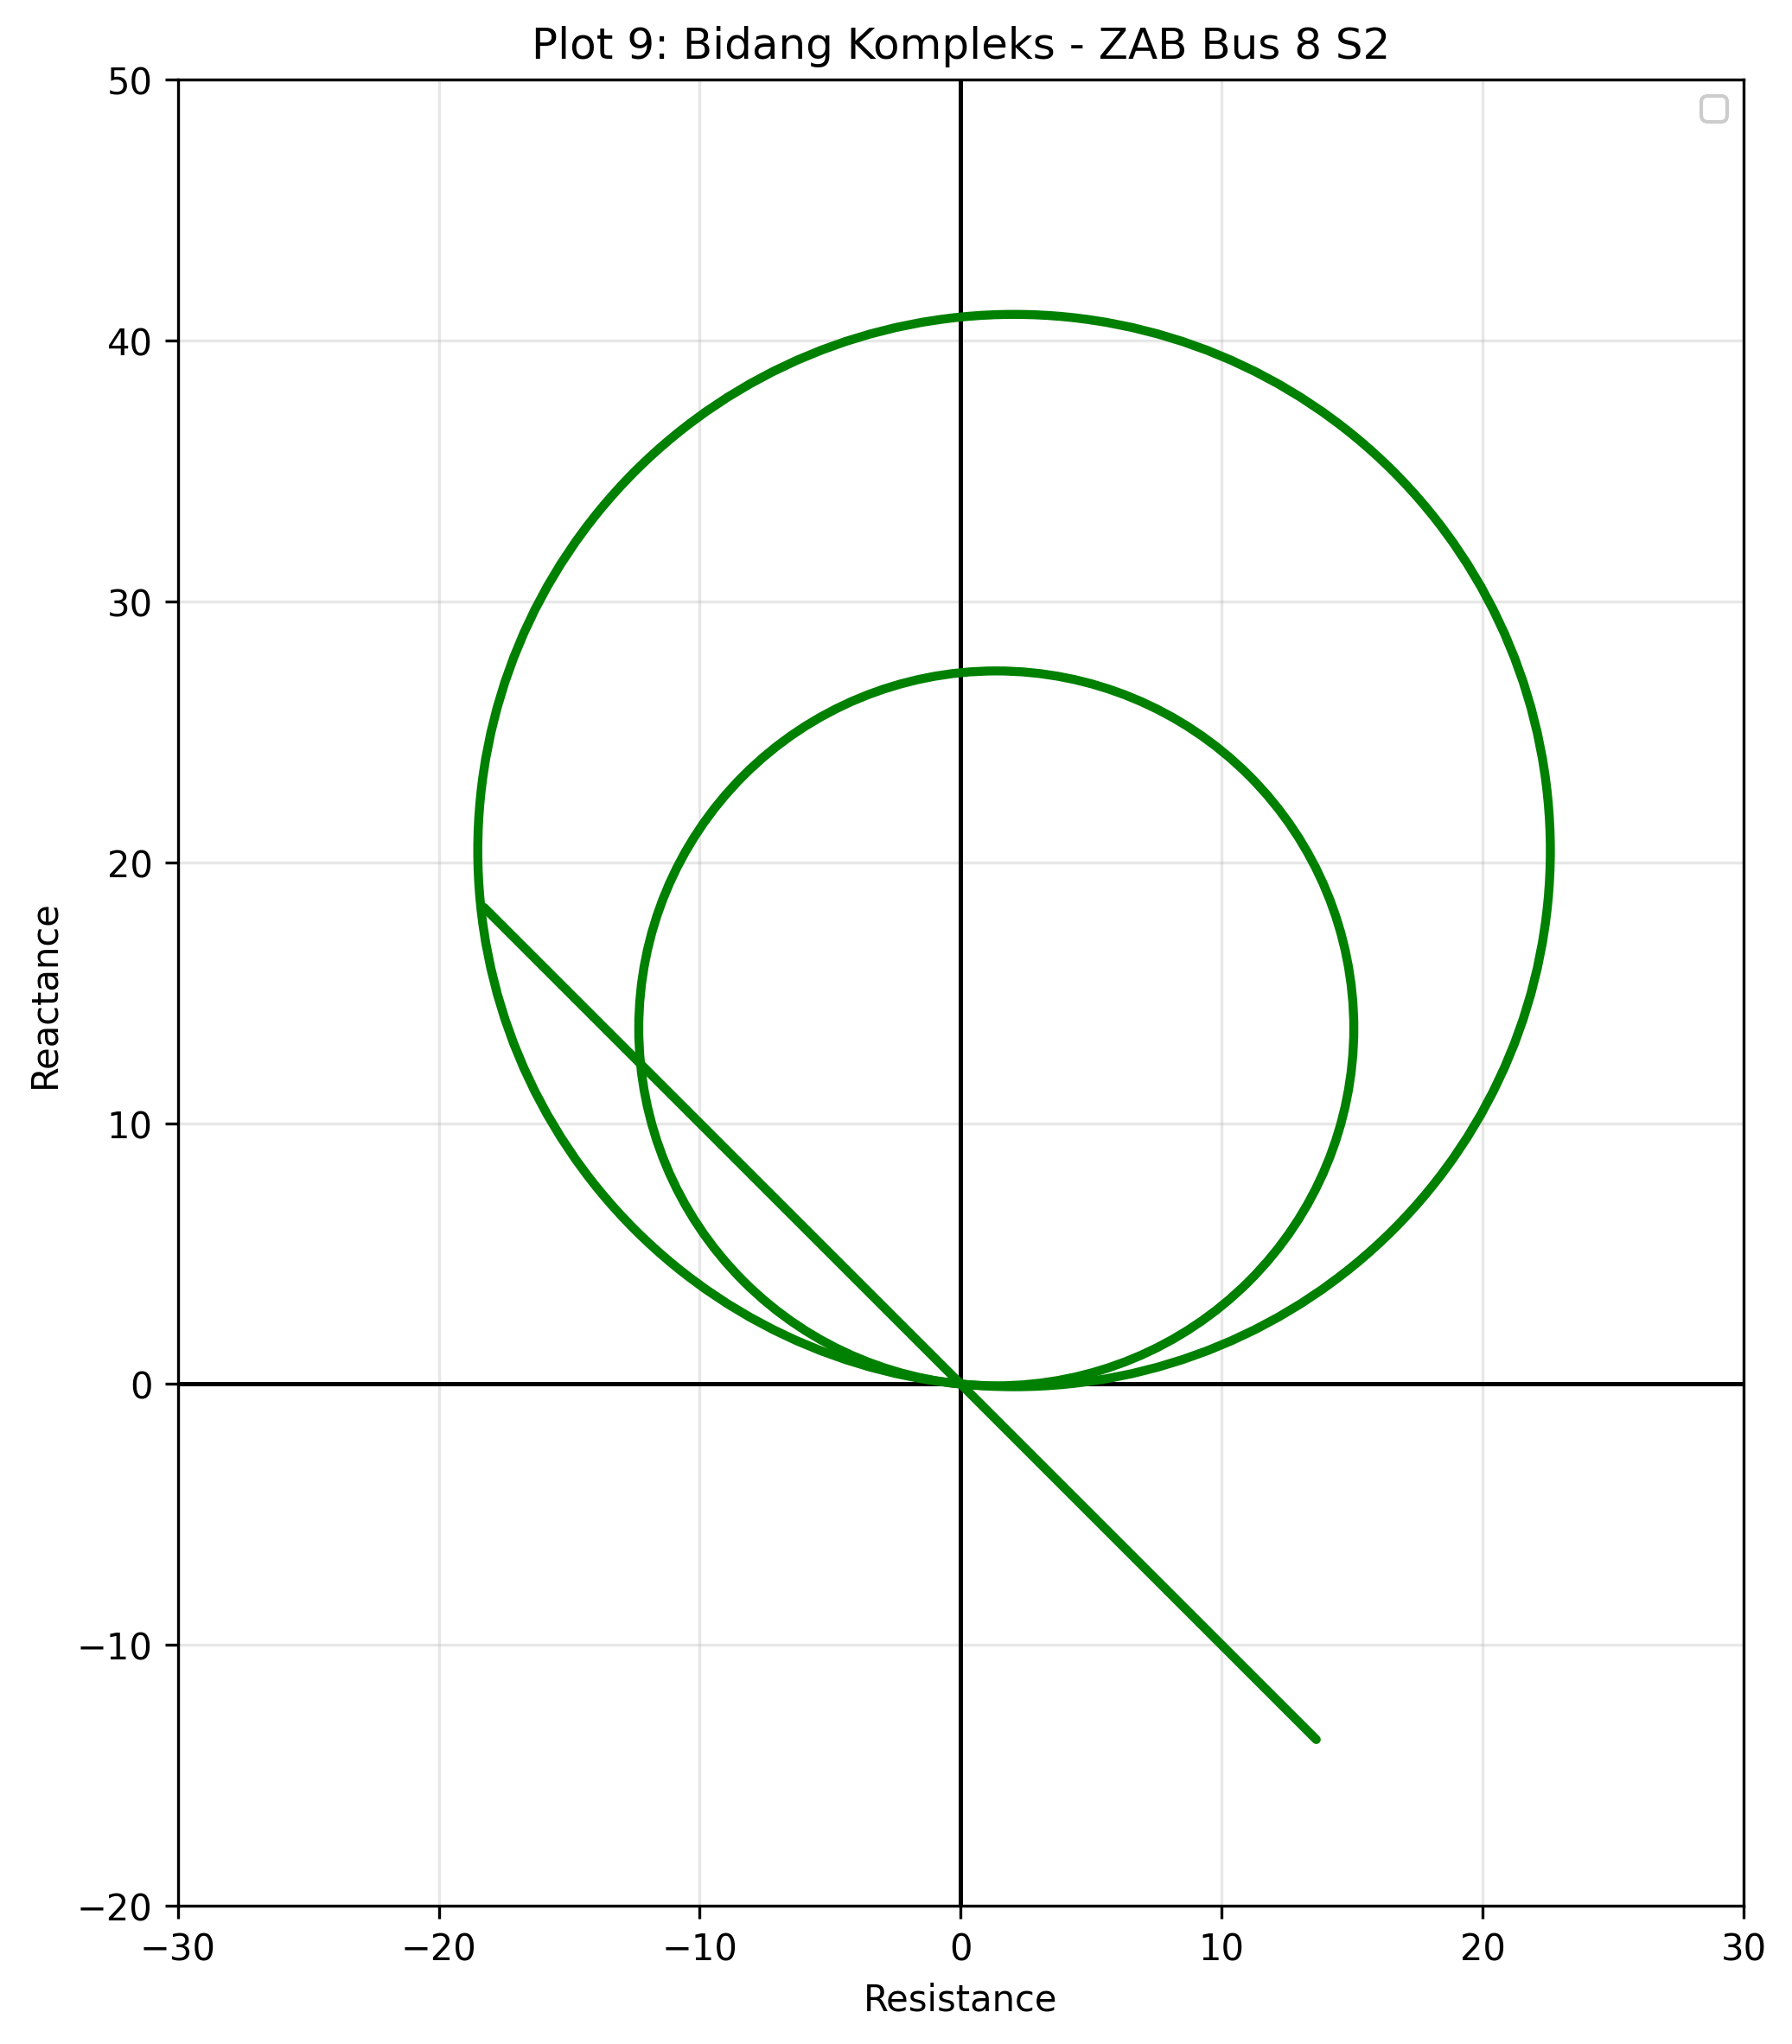
\includegraphics[width=\textwidth]{contents/chapter-4/PRIZI_09_ZAB_Bus_8_S2.png}
        \caption{Zoom In Pada Zona Proteksi}
        \label{fig:PRIZI_09_ZAB_Bus_8_S2}
    \end{subfigure}

    \caption{Impedansi Tampak ZAB Bus 8 Skenario 2}
    \label{fig:Impedansi_Tampak_ZAB_Bus_8_S2}
\end{figure}

Gambar \ref{fig:Impedansi_Tampak_ZAB_Bus_8_S2} menunjukkan bahwa impedansi tampak loop fasa A dengan fasa B yang dibaca oleh relay 21 sisi Bus 8 tidak masuk ke dalam zona proteksi. Sama seperti dua elemen sebelumnya, kondisi ini berkaitan dengan arus sekunder CT pada Gambar \ref{fig:Bus_8_Ex_DLG_S2} yang belum memenuhi syarat \textit{starting} untuk membuat relay aktif. Dengan demikian, berdasarkan acuan gangguan eksternal DLG pada Subbab \ref{subsec:tanpa_IBR_ex_dlg}, respons relay 21 sisi Bus 8 pada skenario 2 menunjukkan \textit{misoperation}.

%%%%%%%%%%%%%%%%%%%%%%%%%%%%%%%%%%%%%%%%%%%%%%%%%%%%%%%%%%%%%%

% \begin{figure}[H]
%     \centering
%     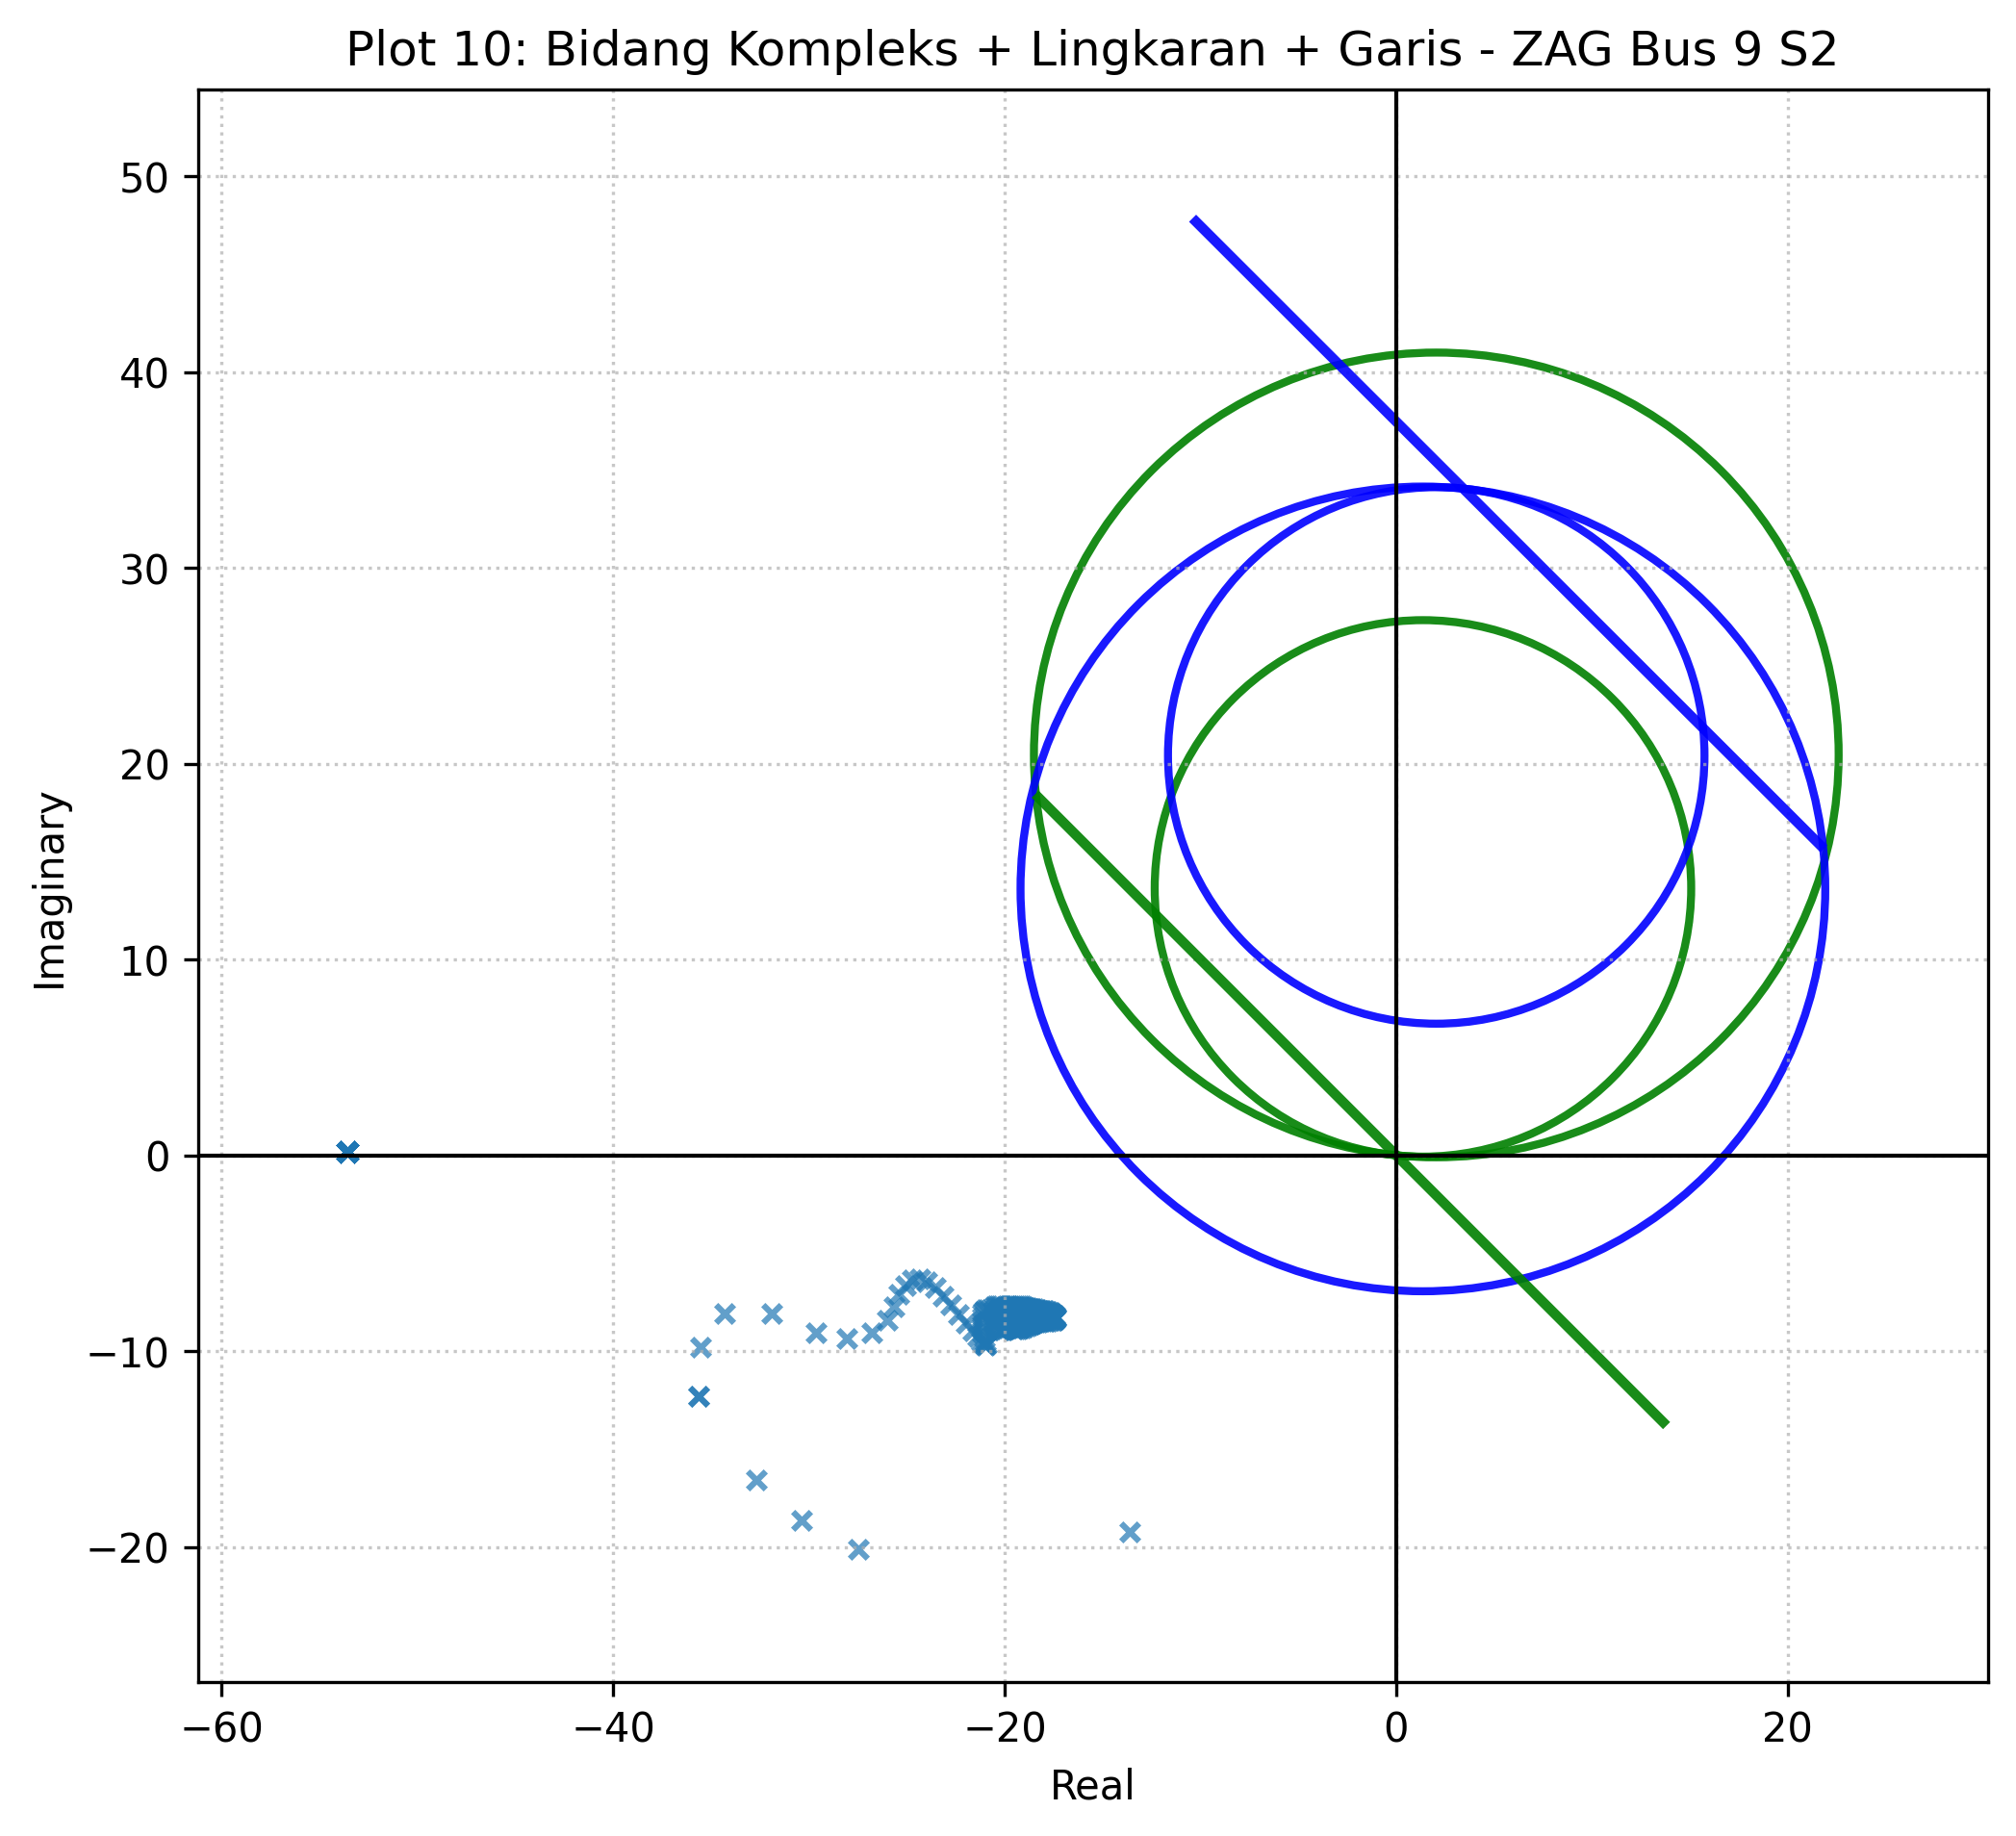
\includegraphics[width=0.8\textwidth]{contents/chapter-4/10_ZAG_Bus_9_S2_dengan_lingkaran_dan_garis.png}
%     \caption{Impedansi Tampak ZAG Bus 9 Skenario 2}
%     \label{fig:10_ZAG_Bus_9_S2_dengan_lingkaran_dan_garis}
% \end{figure}

% Terlihat pada gambar \ref{fig:10_ZAG_Bus_9_S2_dengan_lingkaran_dan_garis} bahwa impedansi tampak pada fasa A dengan ground yang dibaca oleh relay 21 sisi bus 9 saat terdapat gangguan external DLG bekerja dengan baik sesuai acuan pada \ref{subsec:tanpa_IBR_in_dlg} relay 21 bus 9 tidak mendeteksi adanya gangguan sehingga tidak mengirimkan sinyal trip kepada CB.

%%%%%%%%%%%%%%%%%%%%%%%%%%%%%%%%%SISI PRIMER%%%%%%%%%%%%%%%%%%%%%%%%%%%%%%%%%%

% \begin{figure}[H]
%     \centering
%     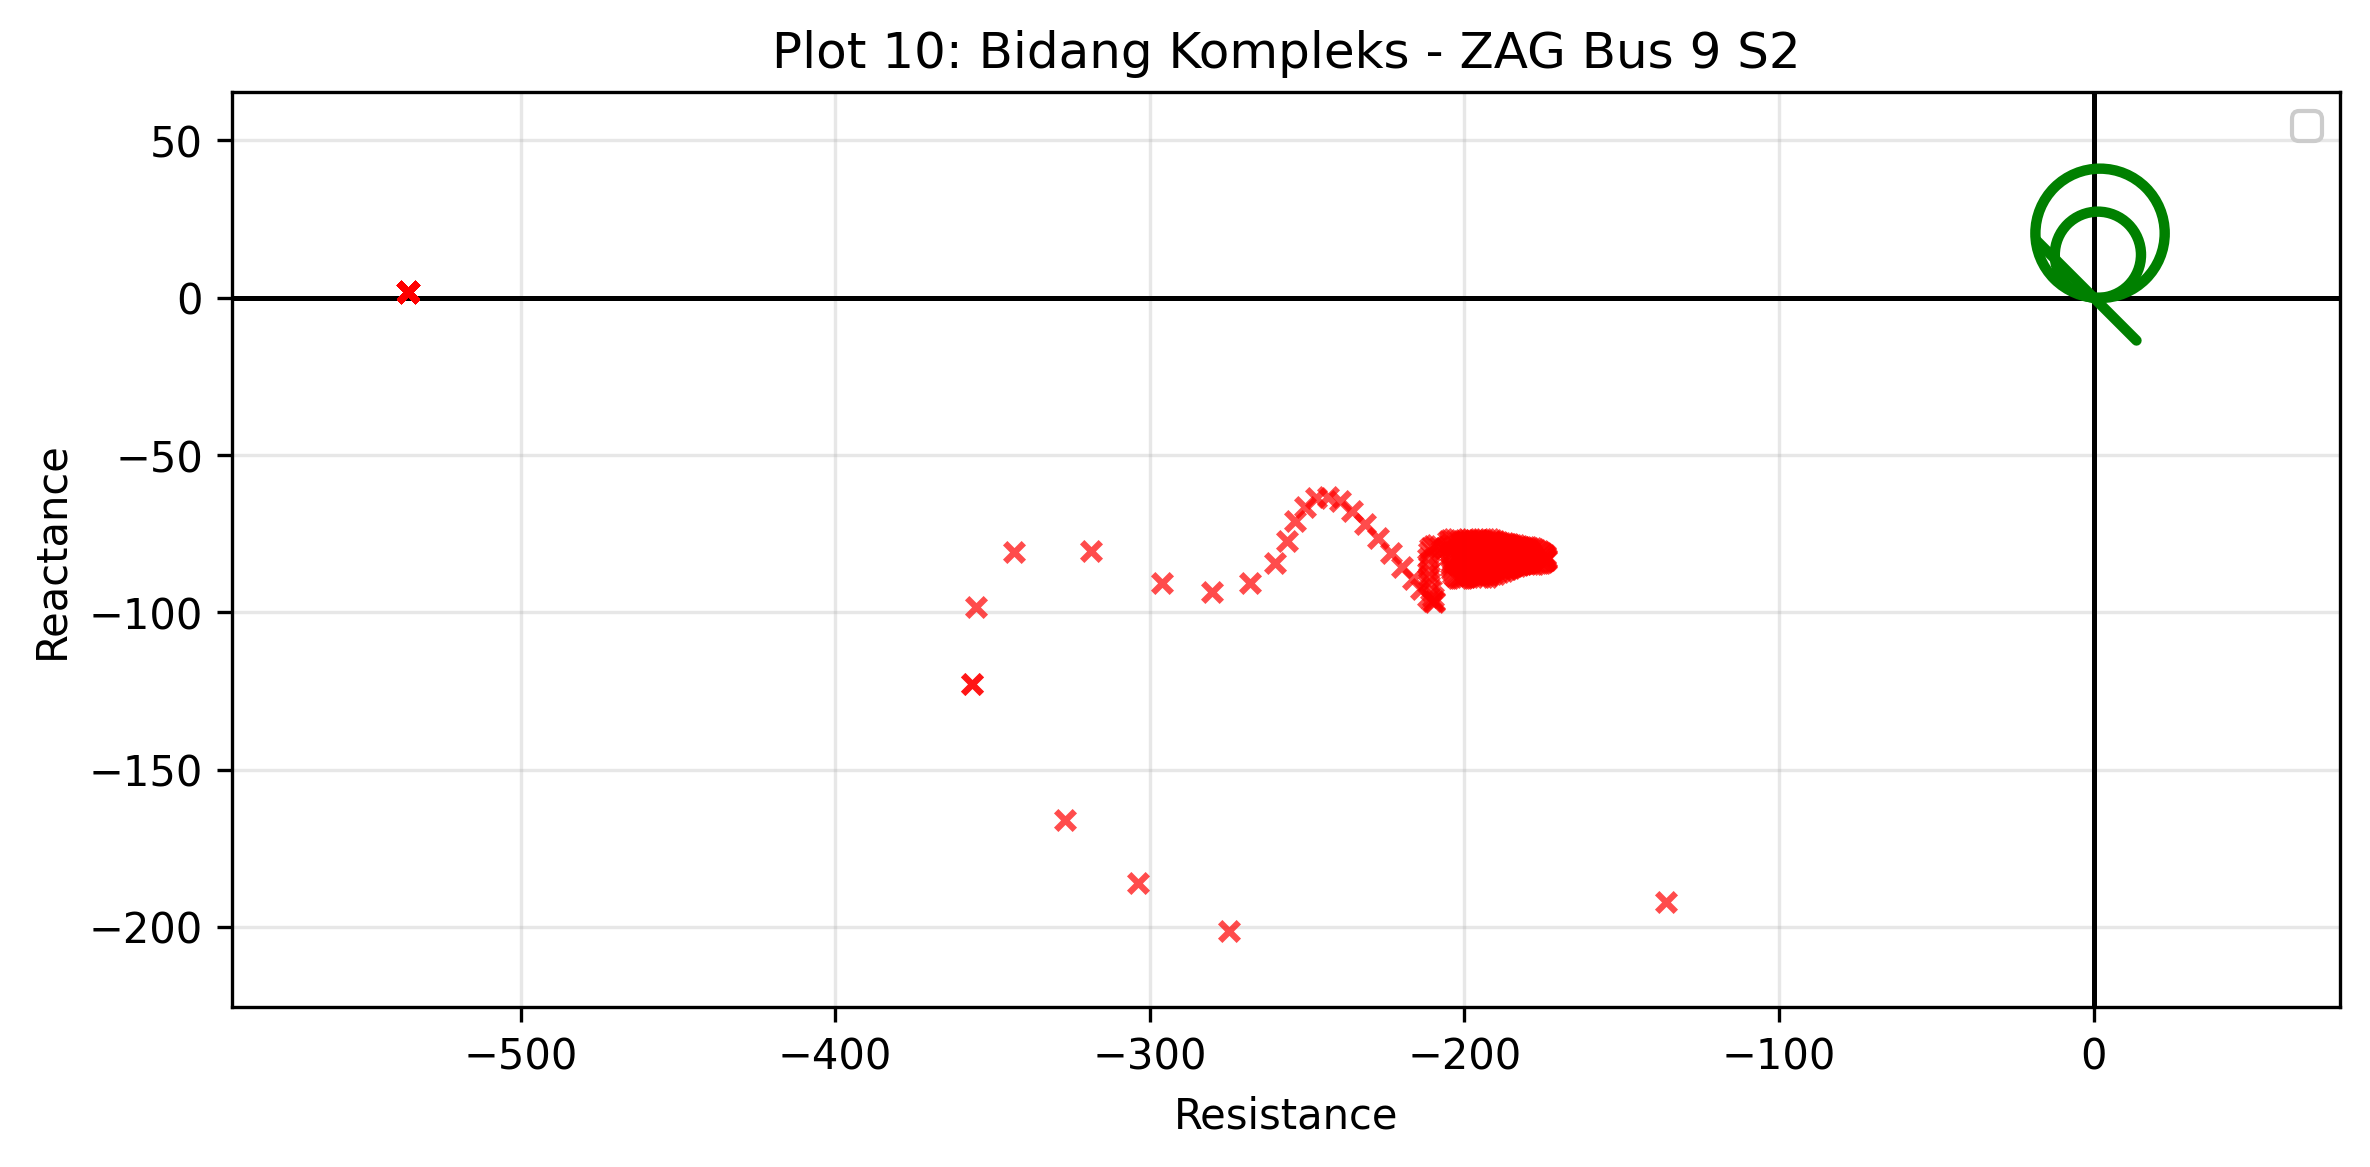
\includegraphics[width=0.8\textwidth]{contents/chapter-4/PRIA_10_ZAG_Bus_9_S2.png}
%     \caption{Impedansi Tampak ZAG Bus 9 Skenario 2}
%     \label{fig:PRIA_10_ZAG_Bus_9_S2}
% \end{figure}

% \begin{figure}[H]
%     \centering
%     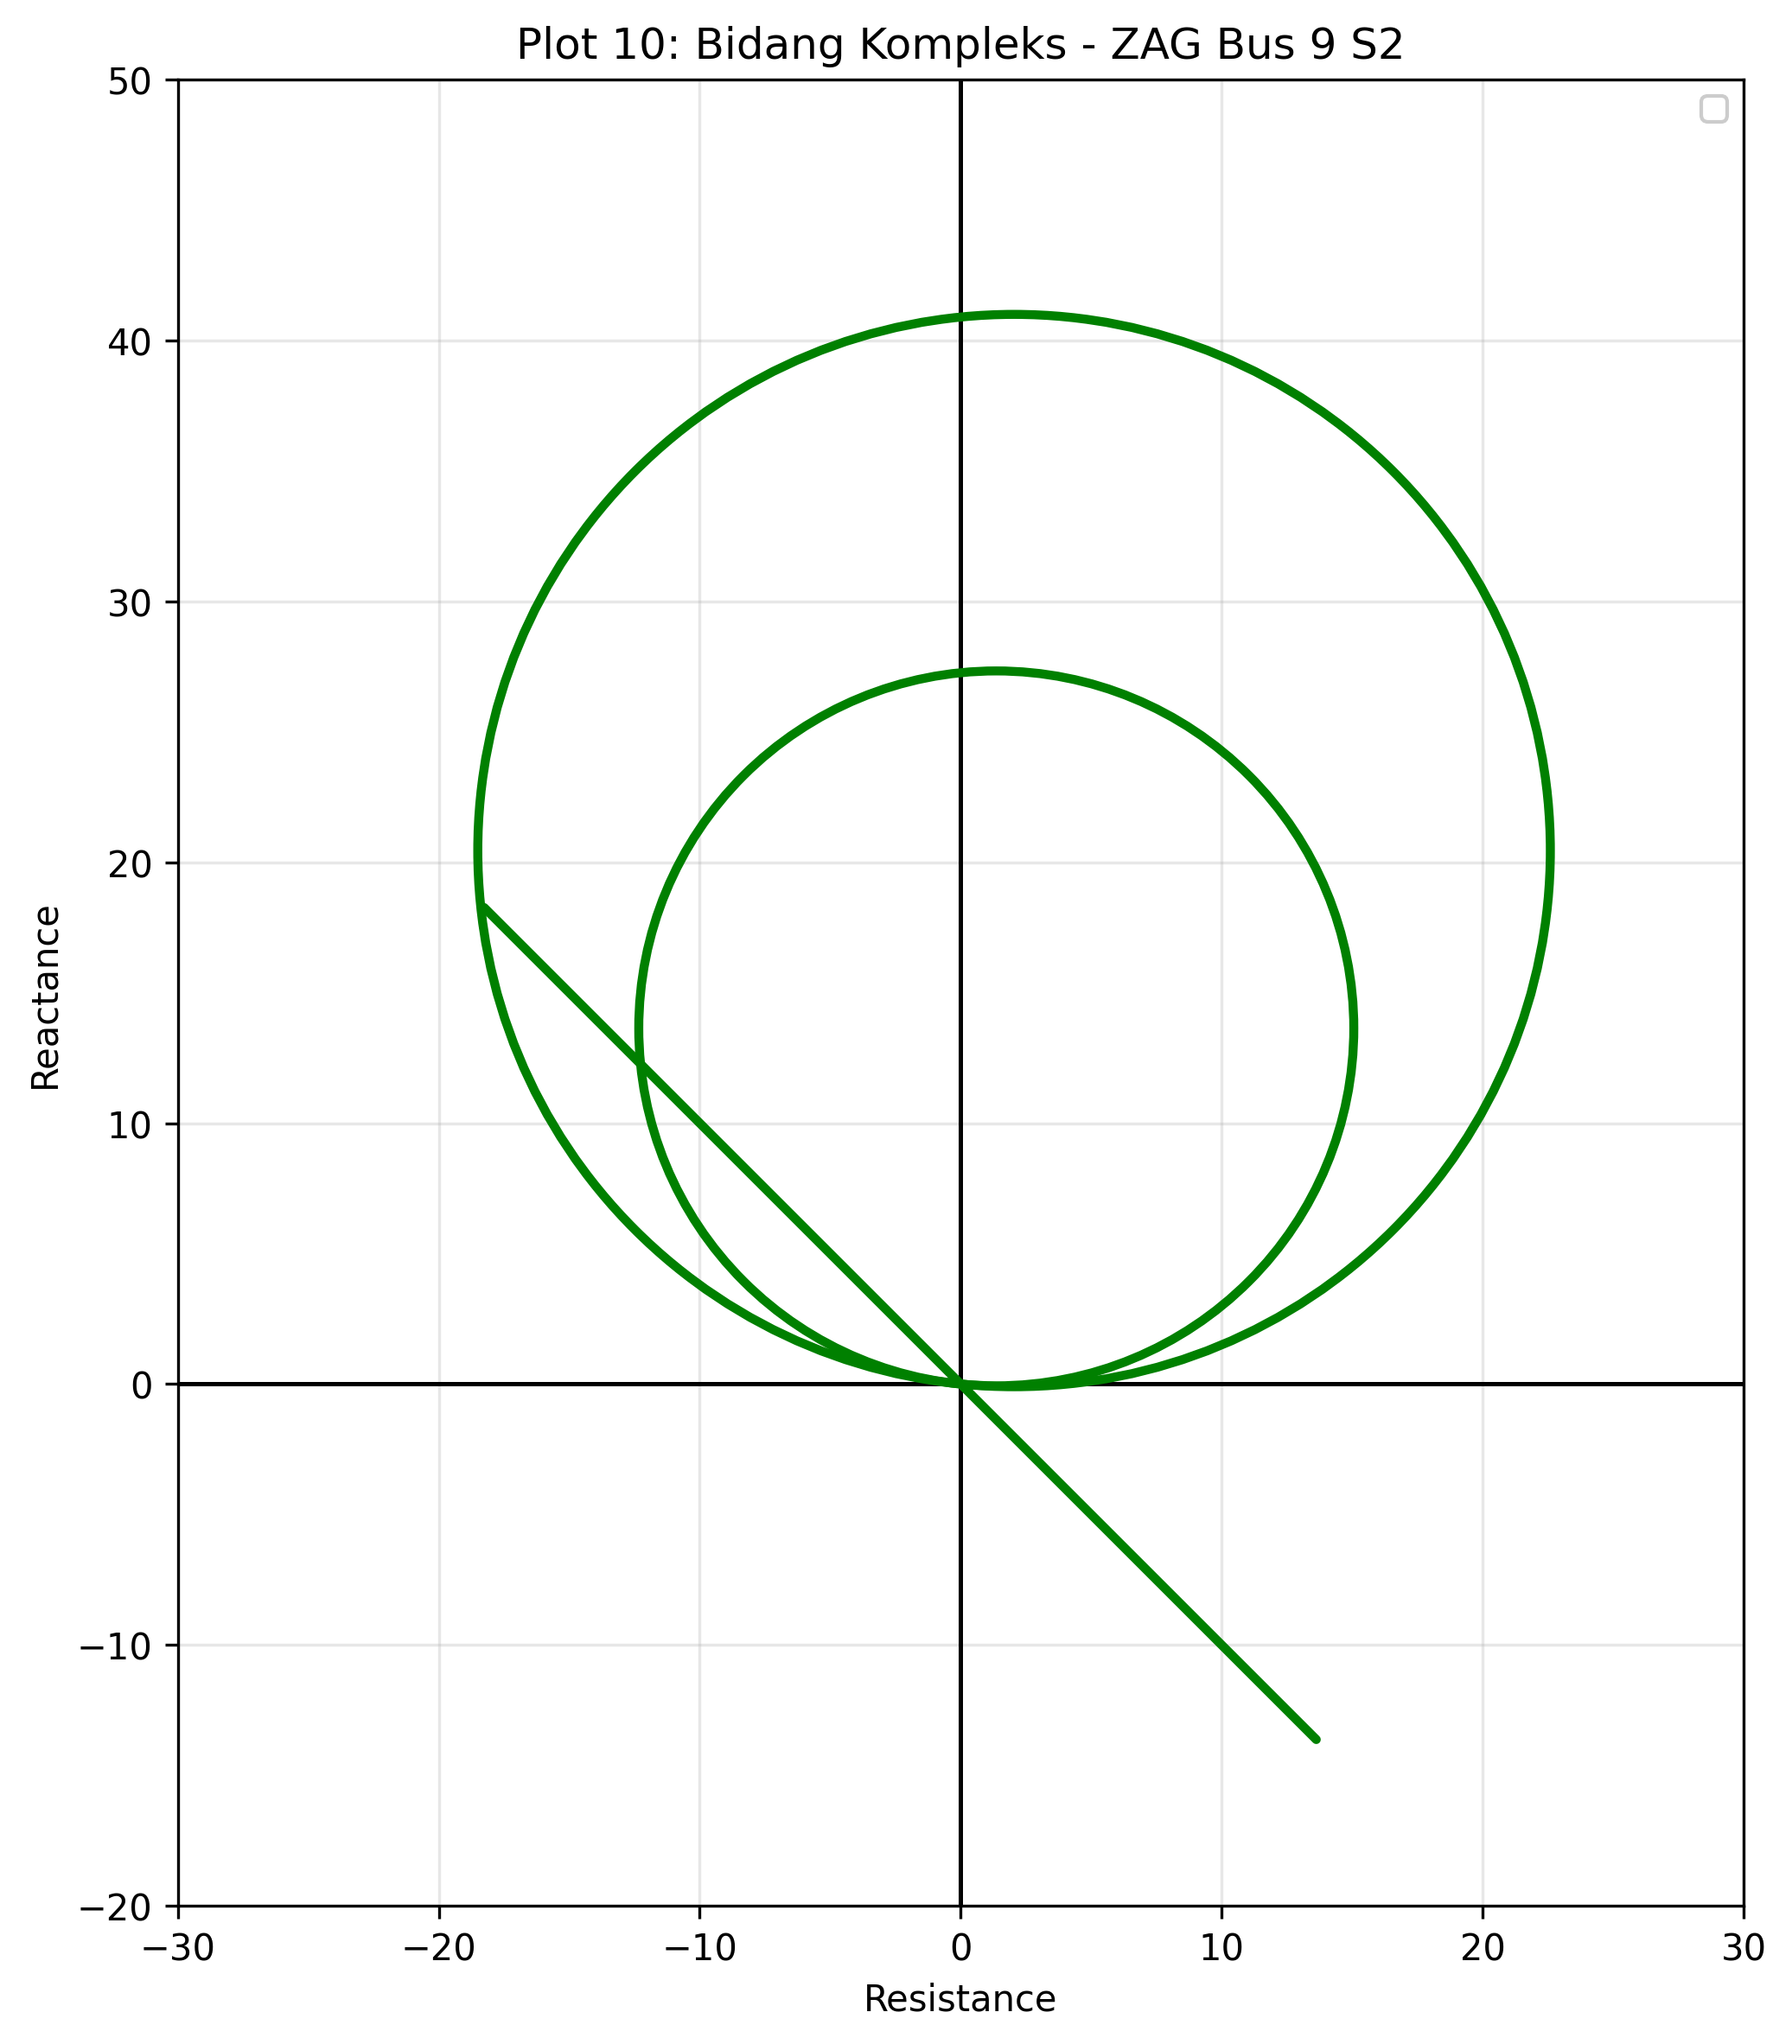
\includegraphics[width=0.8\textwidth]{contents/chapter-4/PRIZI_10_ZAG_Bus_9_S2.png}
%     \caption{Impedansi Tampak ZAG Bus 9 Skenario 2}
%     \label{fig:PRIZI_10_ZAG_Bus_9_S2}
% \end{figure}

\begin{figure}[H]
    \centering

    % Gambar sebelah kiri
    \begin{subfigure}[t]{0.48\textwidth}
        \centering
        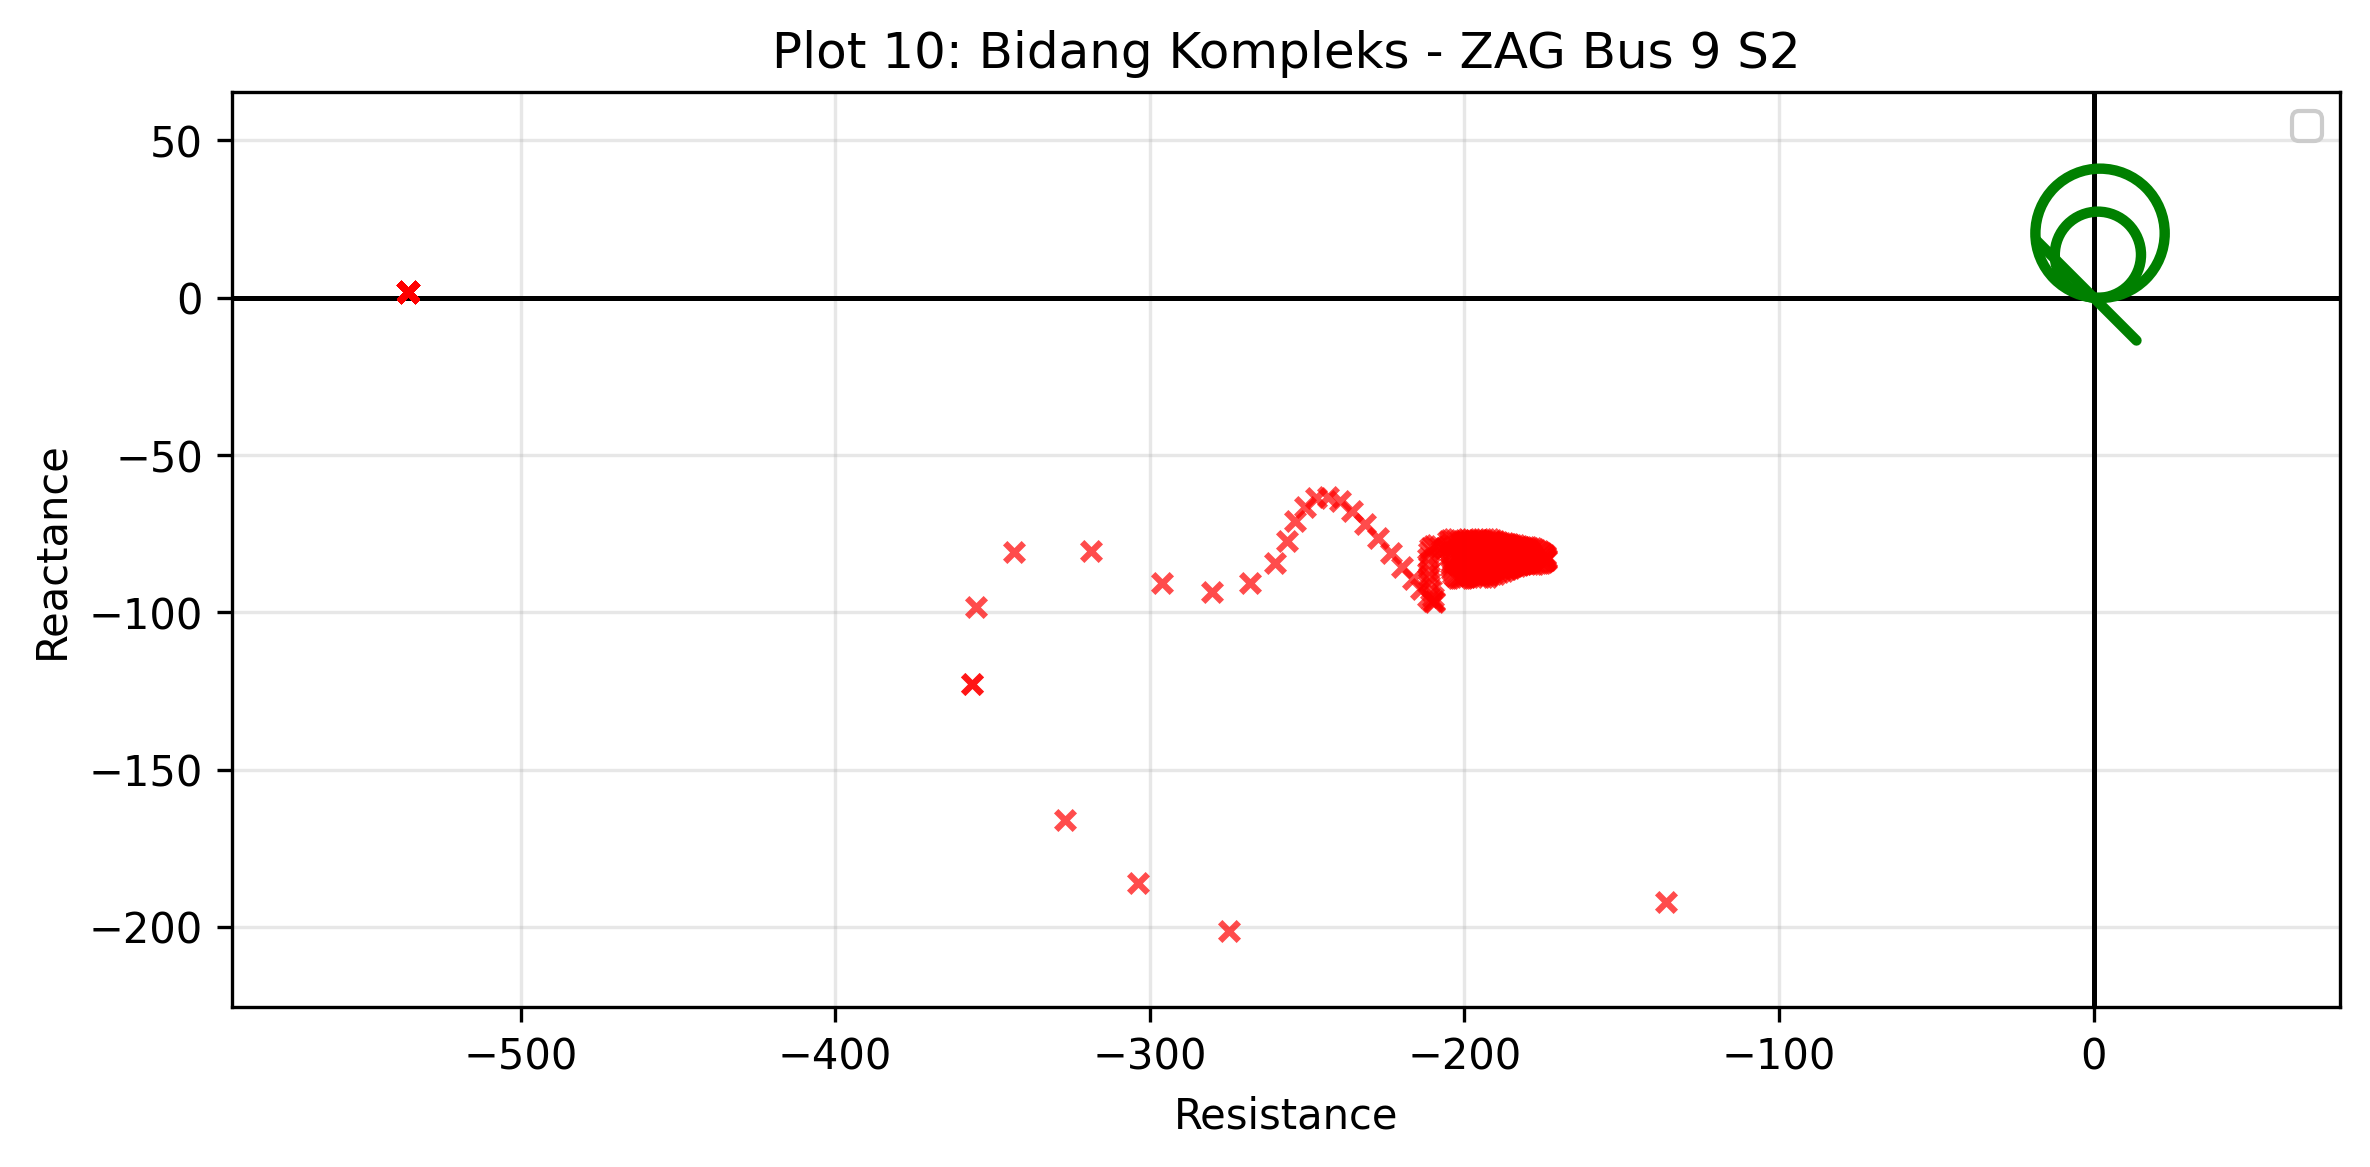
\includegraphics[width=\textwidth]{contents/chapter-4/PRIA_10_ZAG_Bus_9_S2.png}
        \caption{Seluruh Impedansi Tampak}
        \label{fig:PRIA_10_ZAG_Bus_9_S2}
    \end{subfigure}
    \hfill
    % Gambar sebelah kanan
    \begin{subfigure}[t]{0.48\textwidth}
        \centering
        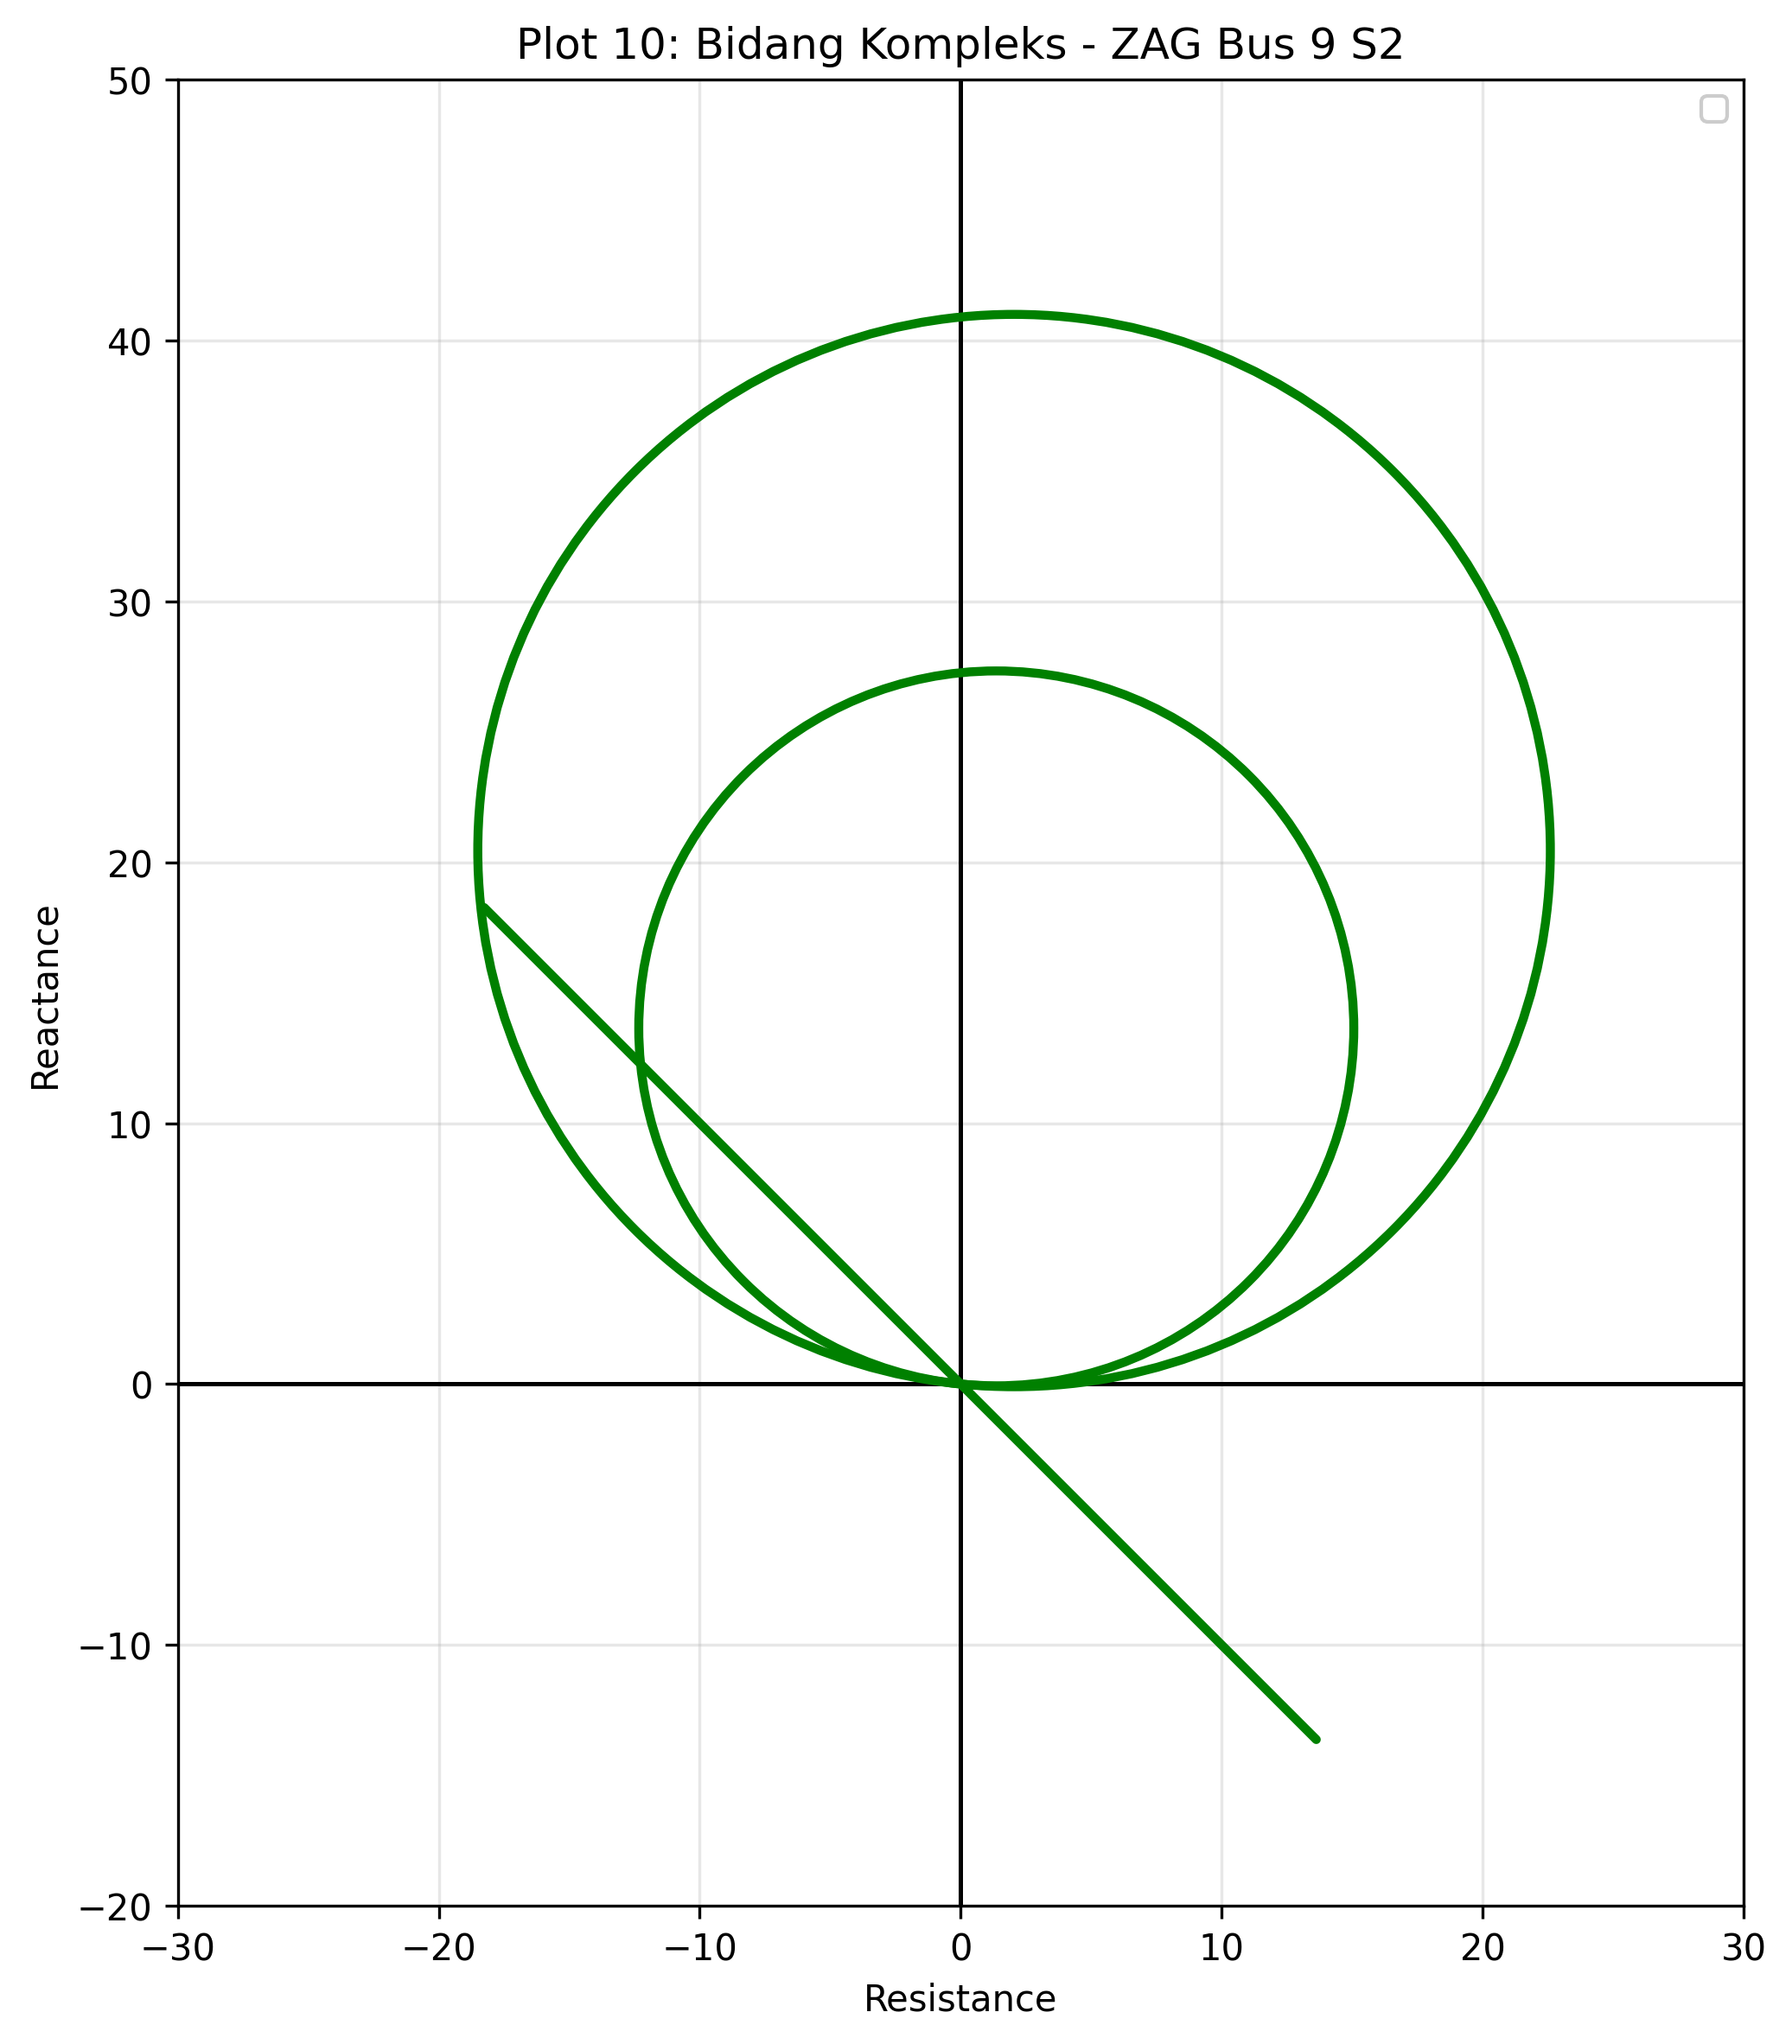
\includegraphics[width=\textwidth]{contents/chapter-4/PRIZI_10_ZAG_Bus_9_S2.png}
        \caption{Zoom In Pada Zona Proteksi}
        \label{fig:PRIZI_10_ZAG_Bus_9_S2}
    \end{subfigure}

    \caption{Impedansi Tampak ZAG Bus 9 Skenario 2}
    \label{fig:Impedansi_Tampak_ZAG_Bus_9_S2}
\end{figure}

Terlihat pada gambar \ref{fig:Impedansi_Tampak_ZAG_Bus_9_S2} bahwa impedansi tampak pada fasa A dengan ground yang dibaca oleh relay 21 sisi bus 9 saat terdapat gangguan bekerja dengan baik sesuai acuan pada \ref{subsec:tanpa_IBR_ex_dlg} relay 21 bus 9 tidak mendeteksi adanya gangguan sehingga tidak mengirimkan sinyal trip kepada CB.


%%%%%%%%%%%%%%%%%%%%%%%%%%%%%%%%%%%%%%%%%%%%%%%%%%%%%%%%%%%%%%

% \begin{figure}[H]
%     \centering
%     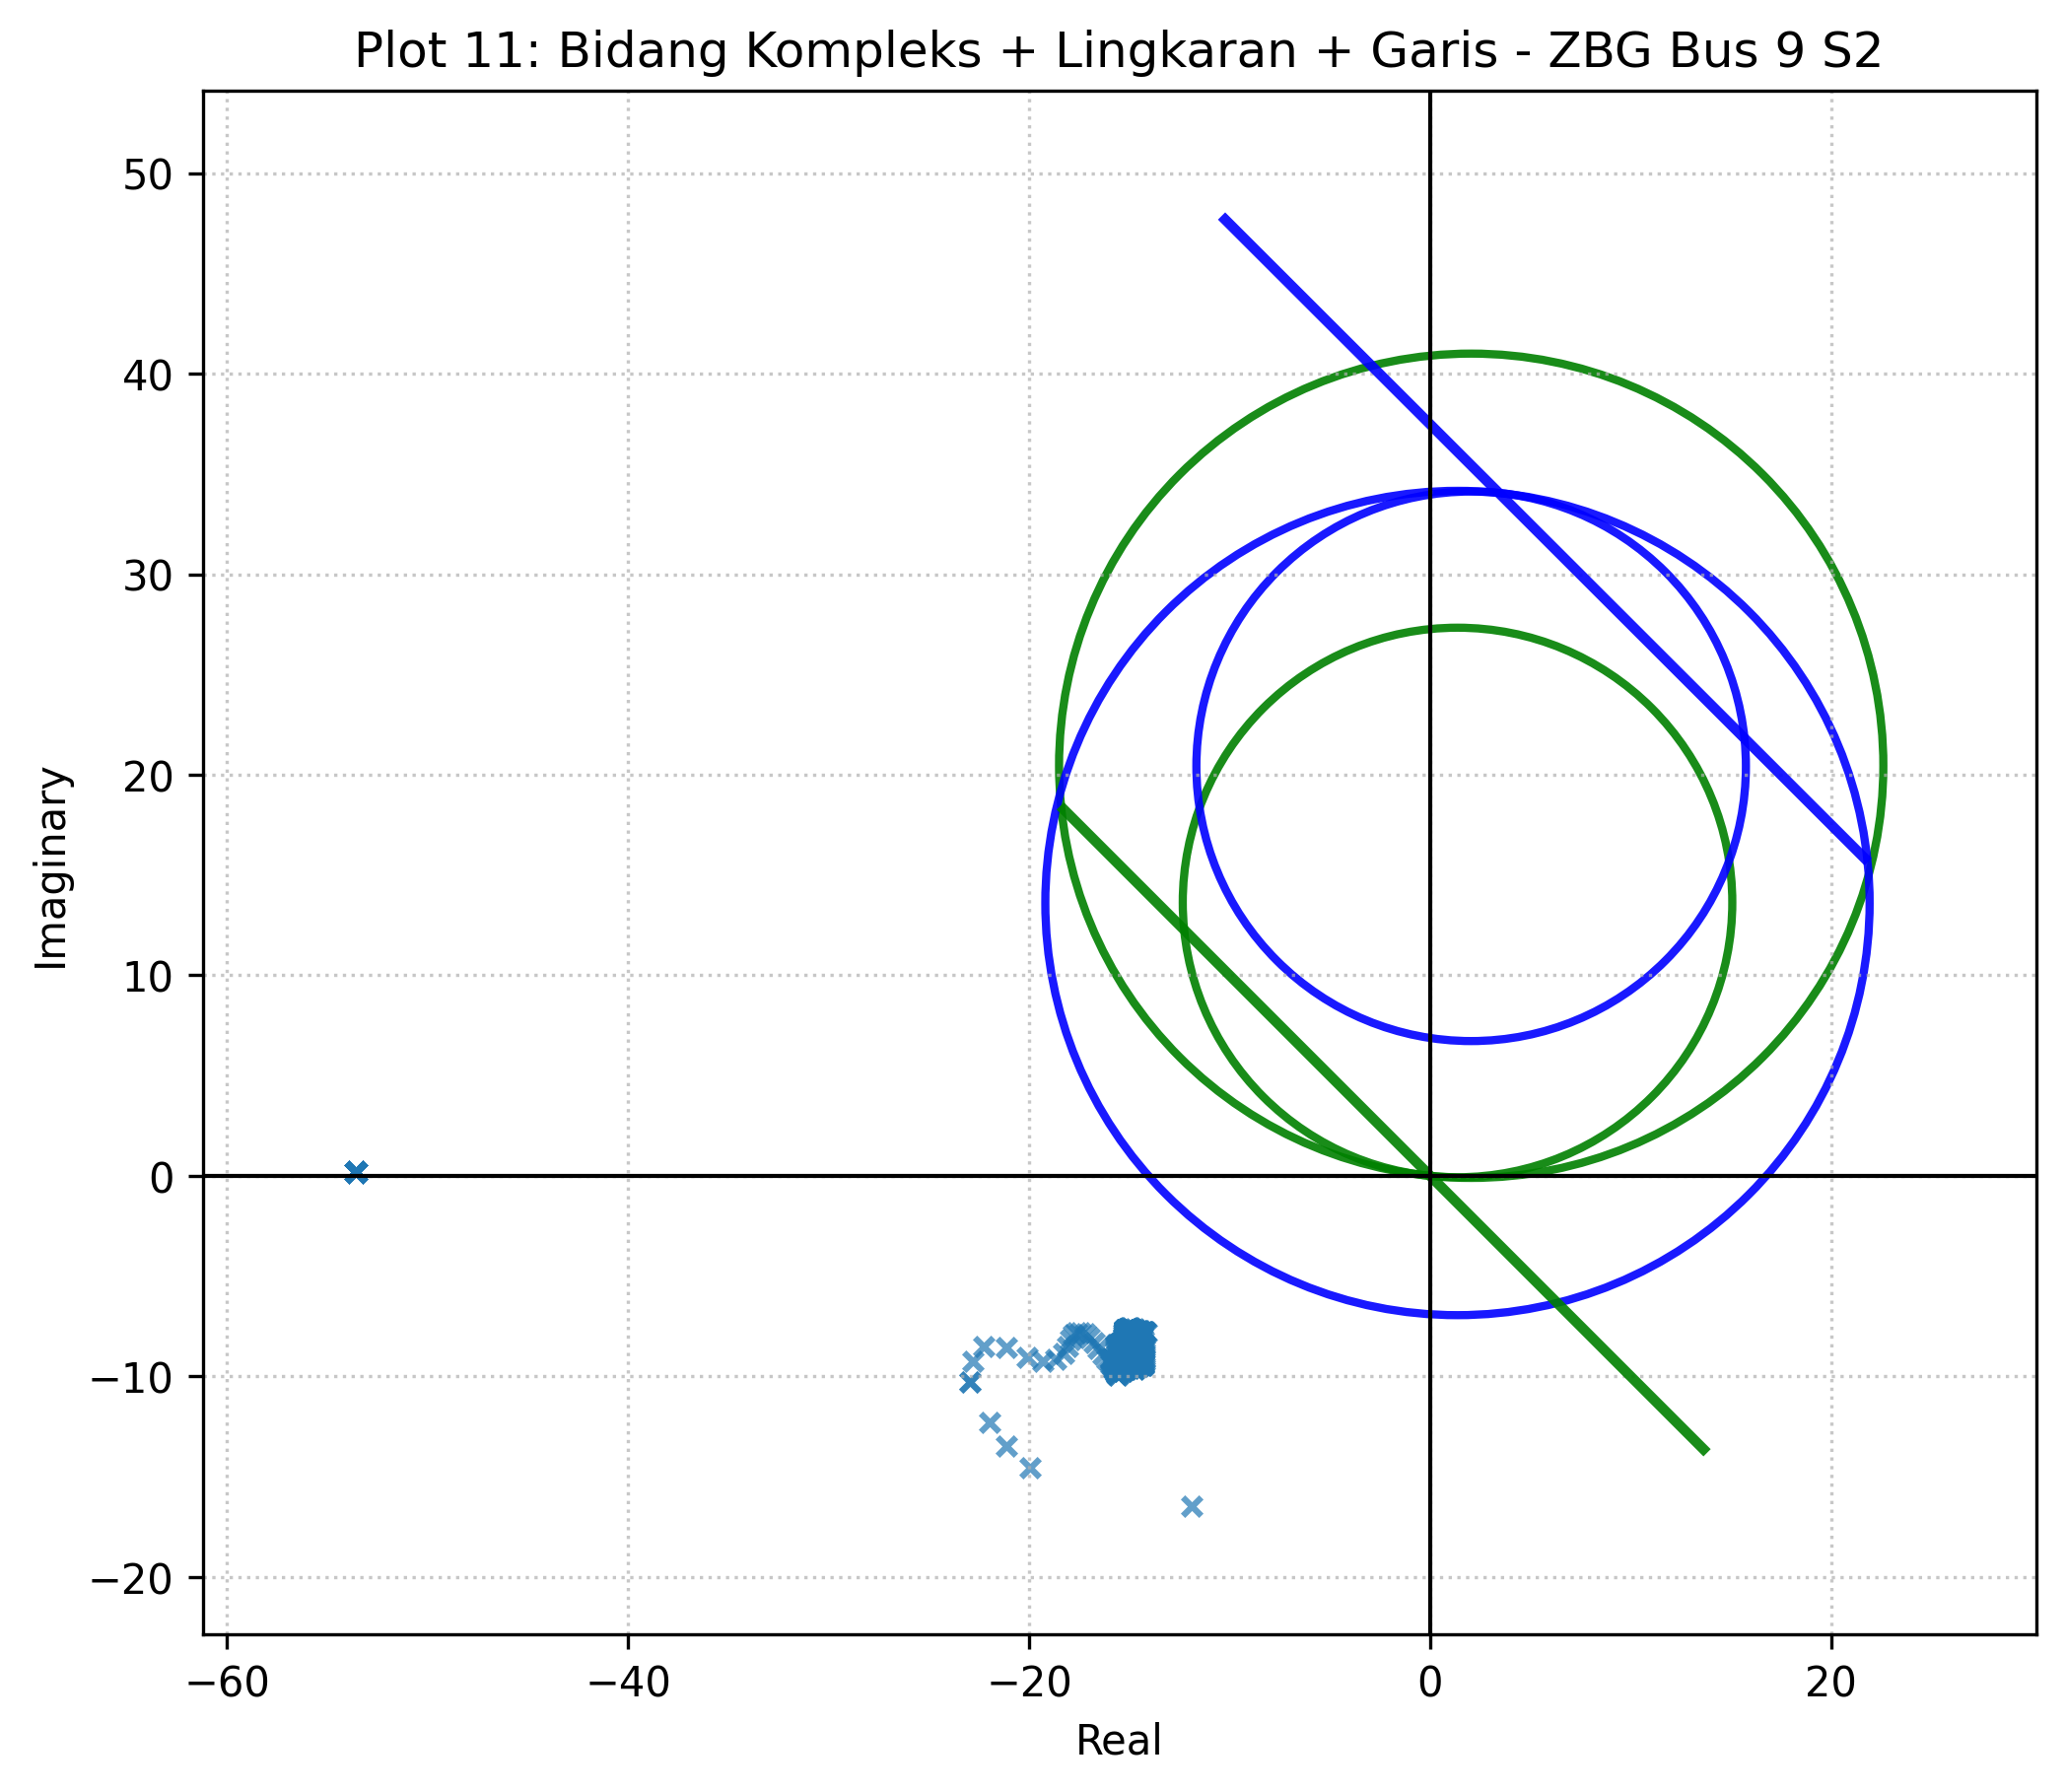
\includegraphics[width=0.8\textwidth]{contents/chapter-4/11_ZBG_Bus_9_S2_dengan_lingkaran_dan_garis.png}
%     \caption{Impedansi Tampak ZBG Bus 9 Skenario 2}
%     \label{fig:11_ZBG_Bus_9_S2_dengan_lingkaran_dan_garis}
% \end{figure}

% Terlihat pada gambar \ref{fig:11_ZBG_Bus_9_S2_dengan_lingkaran_dan_garis} bahwa impedansi tampak pada fasa B dengan ground yang dibaca oleh relay 21 sisi bus 9 saat terdapat gangguan external DLG bekerja dengan baik sesuai acuan pada \ref{subsec:tanpa_IBR_in_dlg} relay 21 bus 9 tidak mendeteksi adanya gangguan sehingga tidak mengirimkan sinyal trip kepada CB.

%%%%%%%%%%%%%%%%%%%%%%%%%%%%%%%%%SISI PRIMER%%%%%%%%%%%%%%%%%%%%%%%%%%%%%%%%%%

% \begin{figure}[H]
%     \centering
%     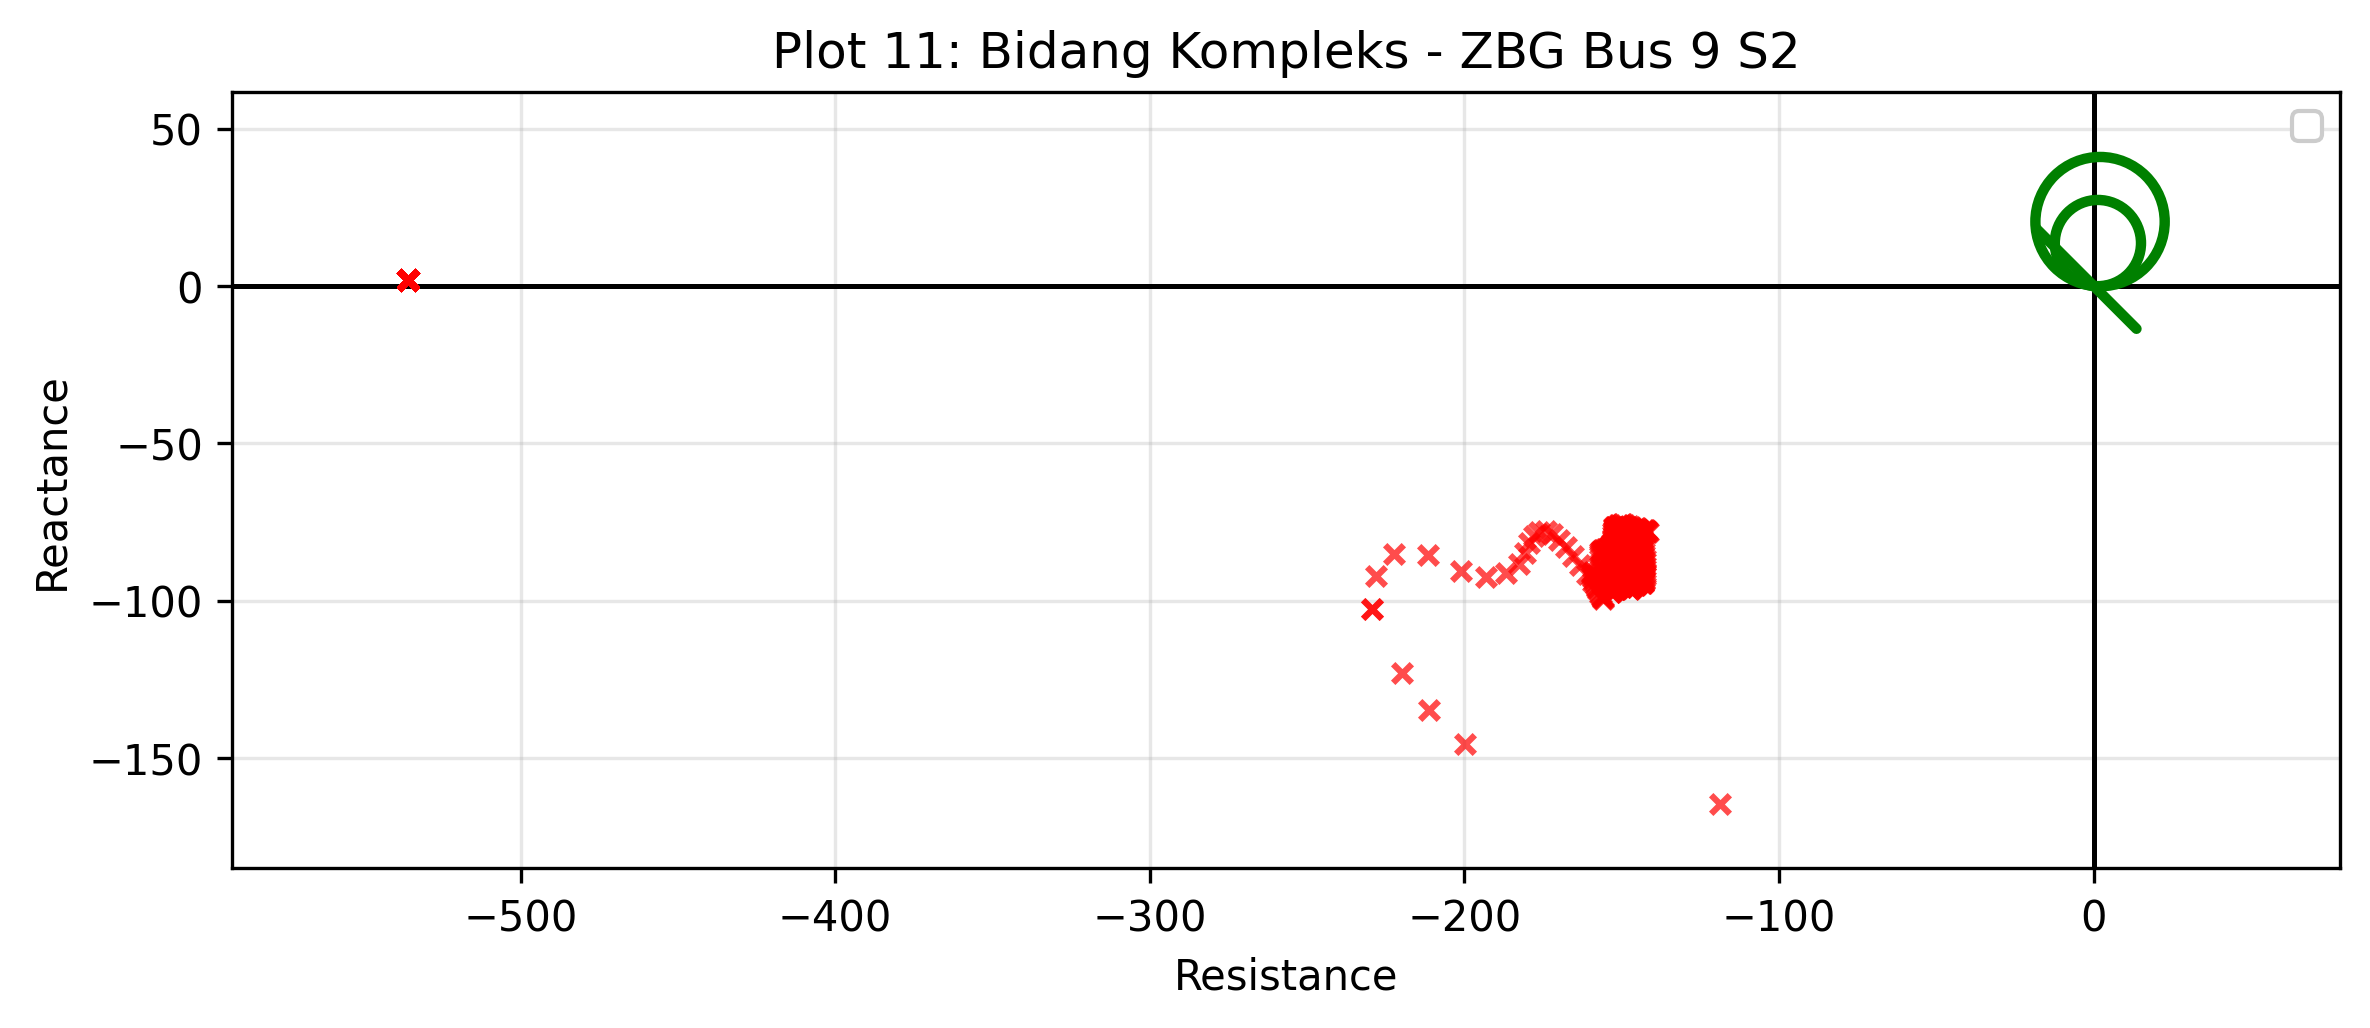
\includegraphics[width=0.8\textwidth]{contents/chapter-4/PRIA_11_ZBG_Bus_9_S2.png}
%     \caption{Impedansi Tampak ZBG Bus 9 Skenario 2}
%     \label{fig:PRIA_11_ZBG_Bus_9_S2}
% \end{figure}

% \begin{figure}[H]
%     \centering
%     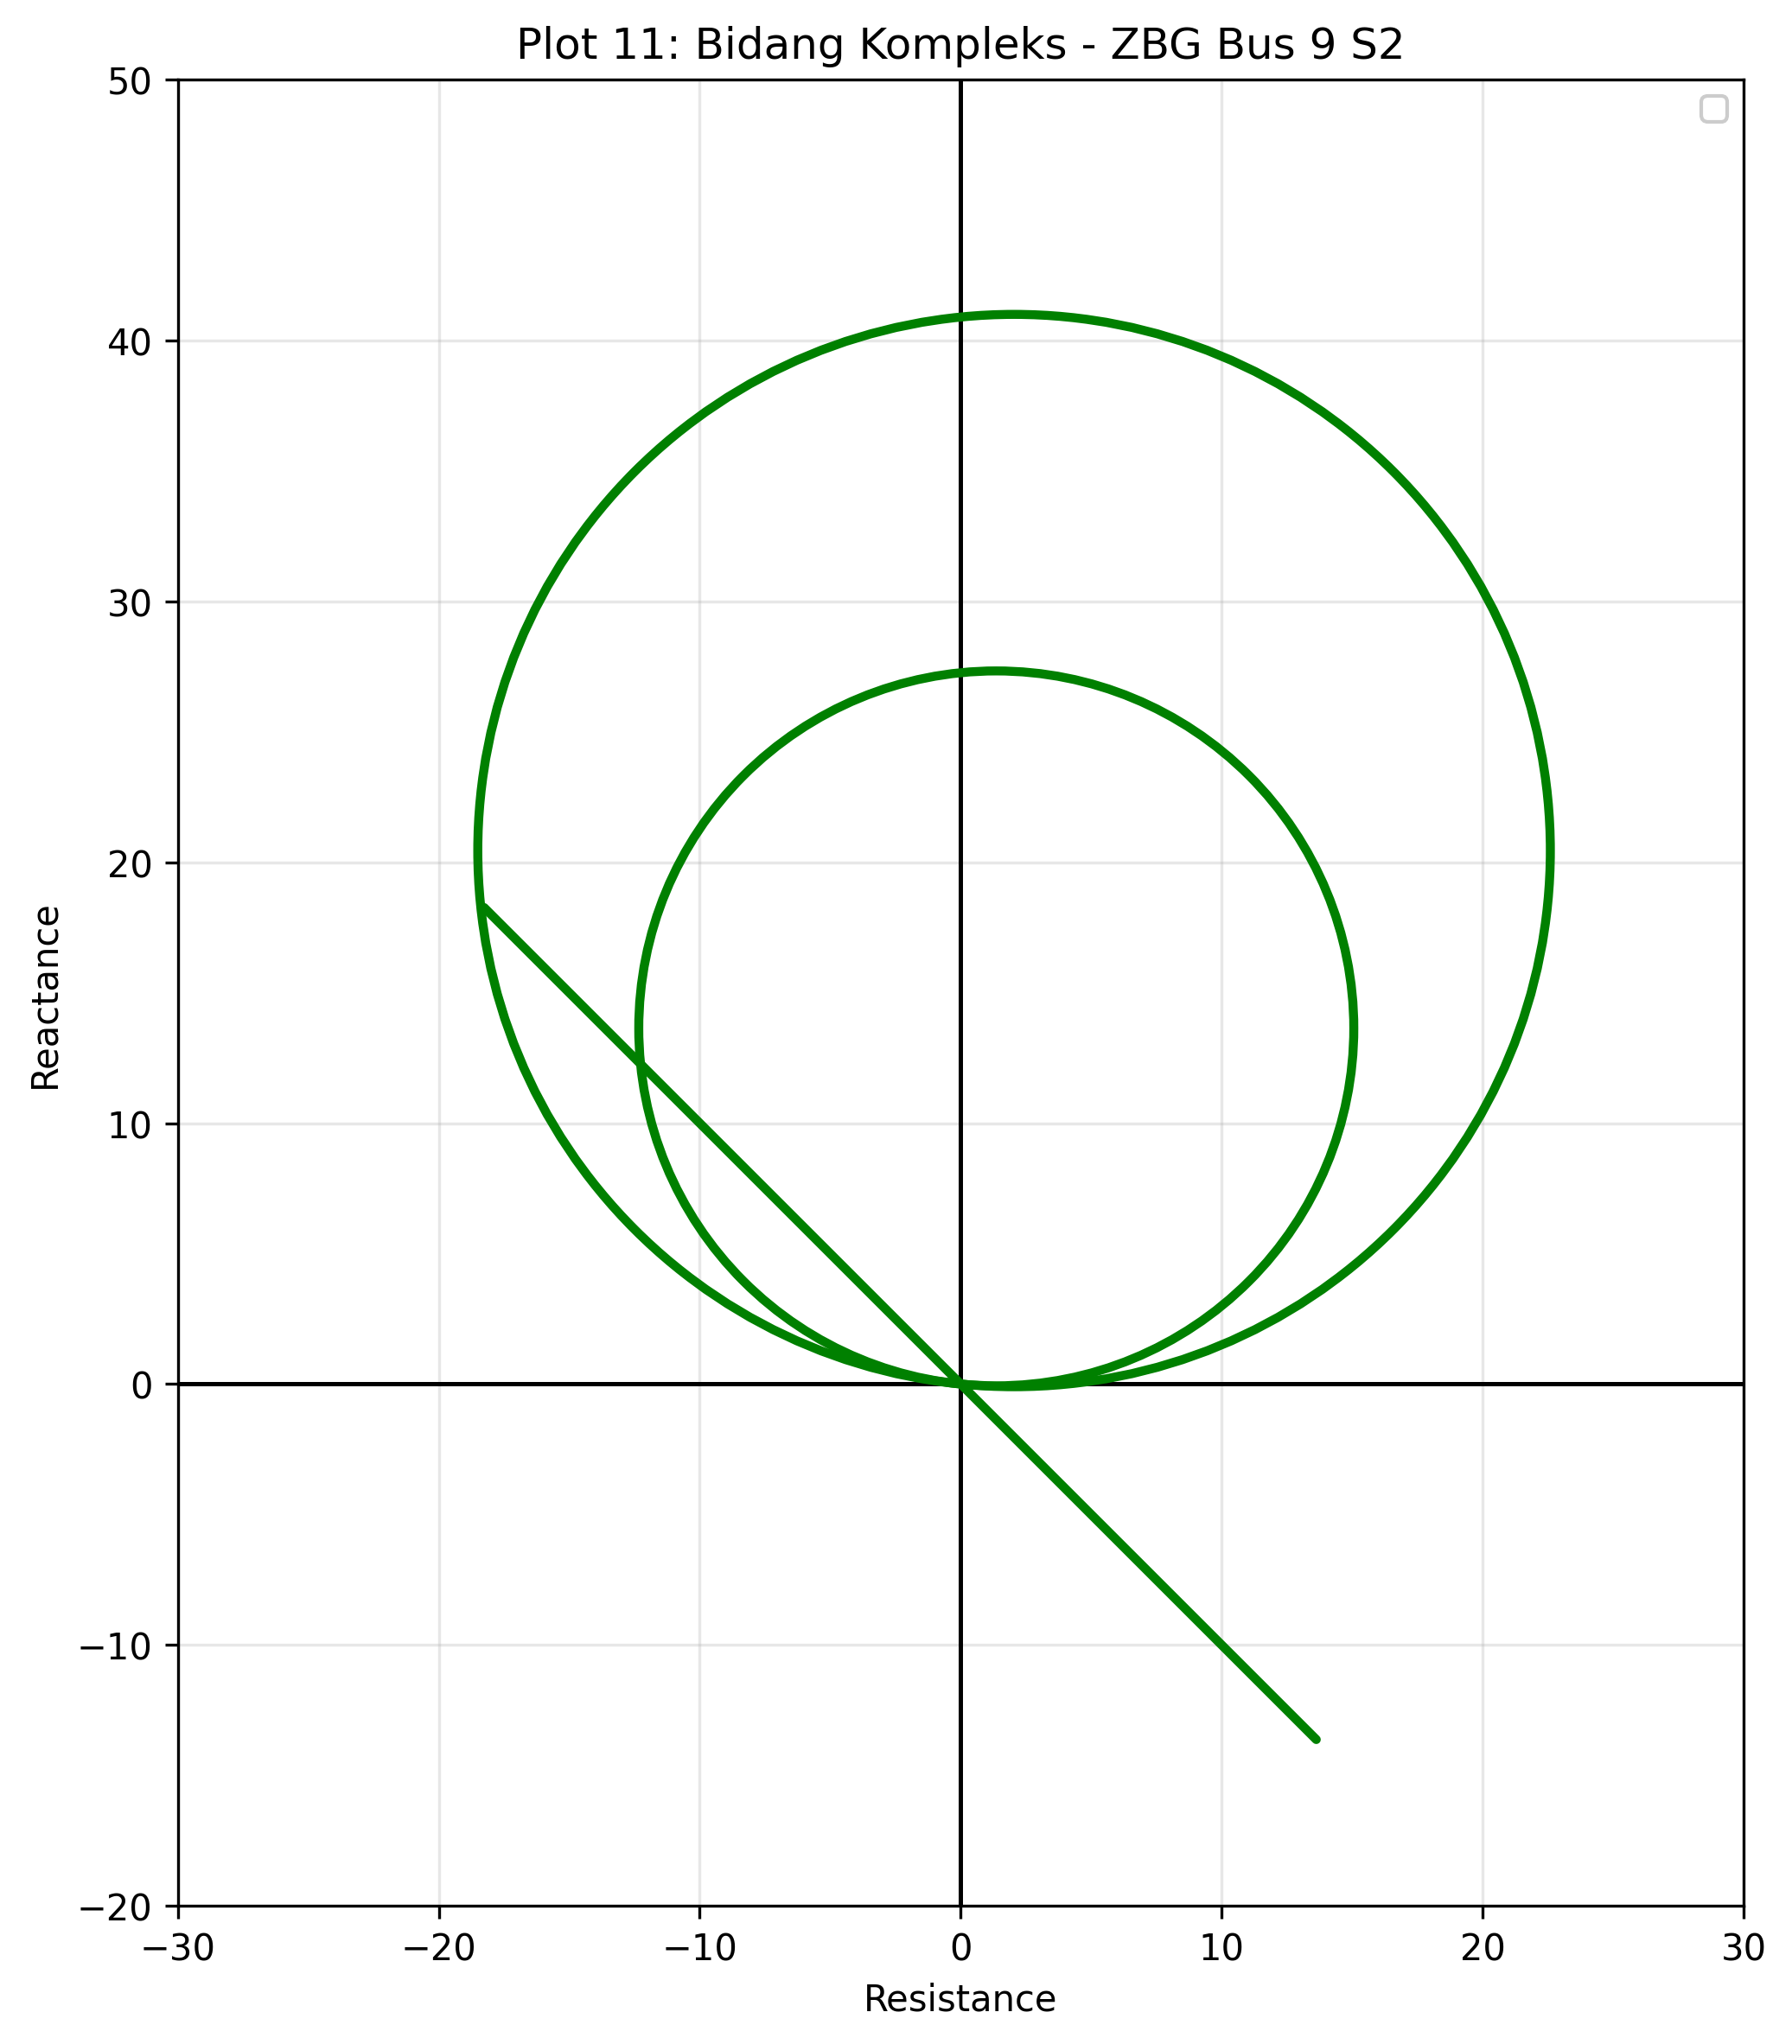
\includegraphics[width=0.8\textwidth]{contents/chapter-4/PRIZI_11_ZBG_Bus_9_S2.png}
%     \caption{Impedansi Tampak ZBG Bus 9 Skenario 2}
%     \label{fig:PRIZI_11_ZBG_Bus_9_S2}
% \end{figure}

\begin{figure}[H]
    \centering

    % Gambar sebelah kiri
    \begin{subfigure}[t]{0.48\textwidth}
        \centering
        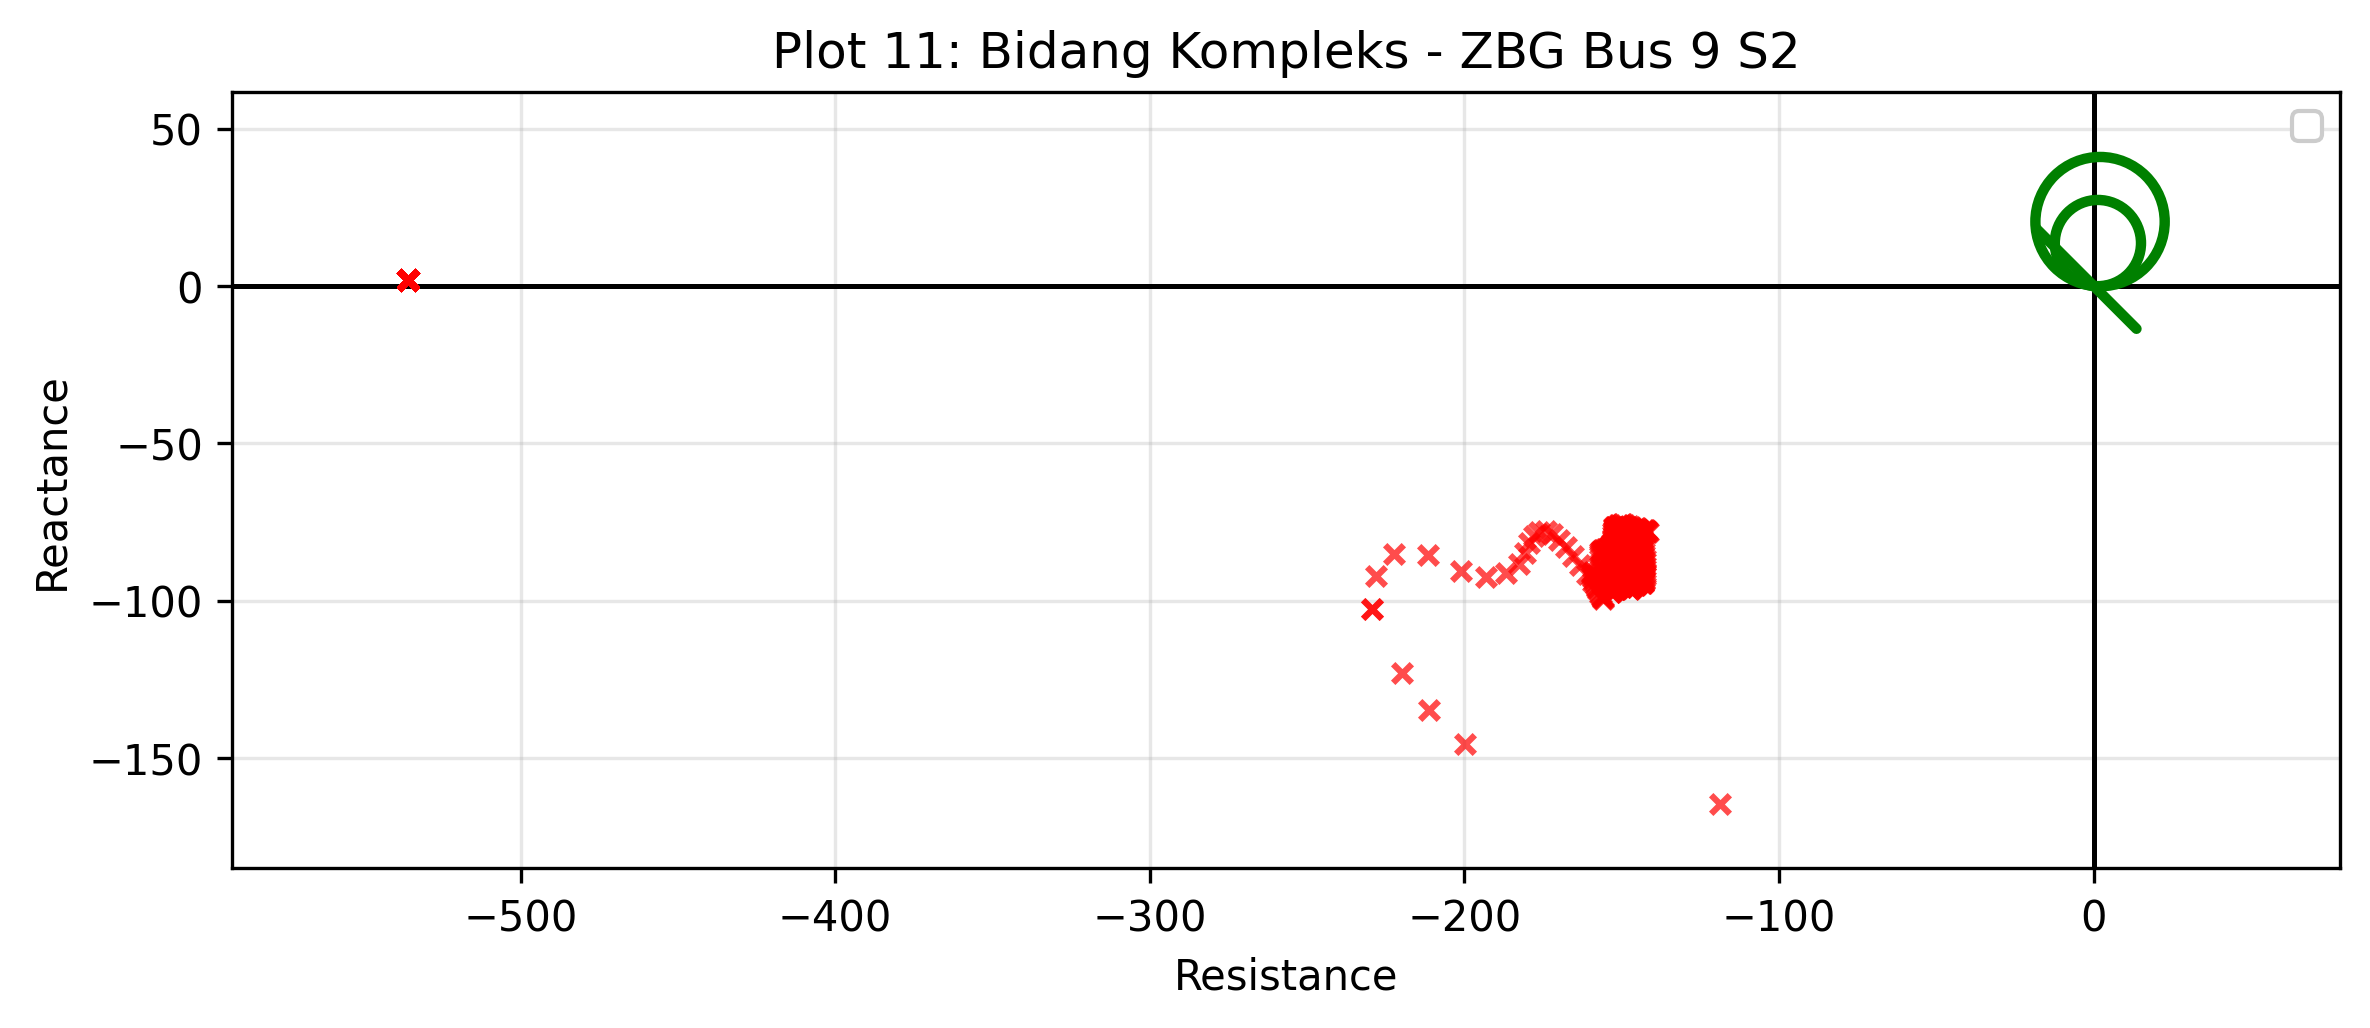
\includegraphics[width=\textwidth]{contents/chapter-4/PRIA_11_ZBG_Bus_9_S2.png}
        \caption{Seluruh Impedansi Tampak}
        \label{fig:PRIA_11_ZBG_Bus_9_S2}
    \end{subfigure}
    \hfill
    % Gambar sebelah kanan
    \begin{subfigure}[t]{0.48\textwidth}
        \centering
        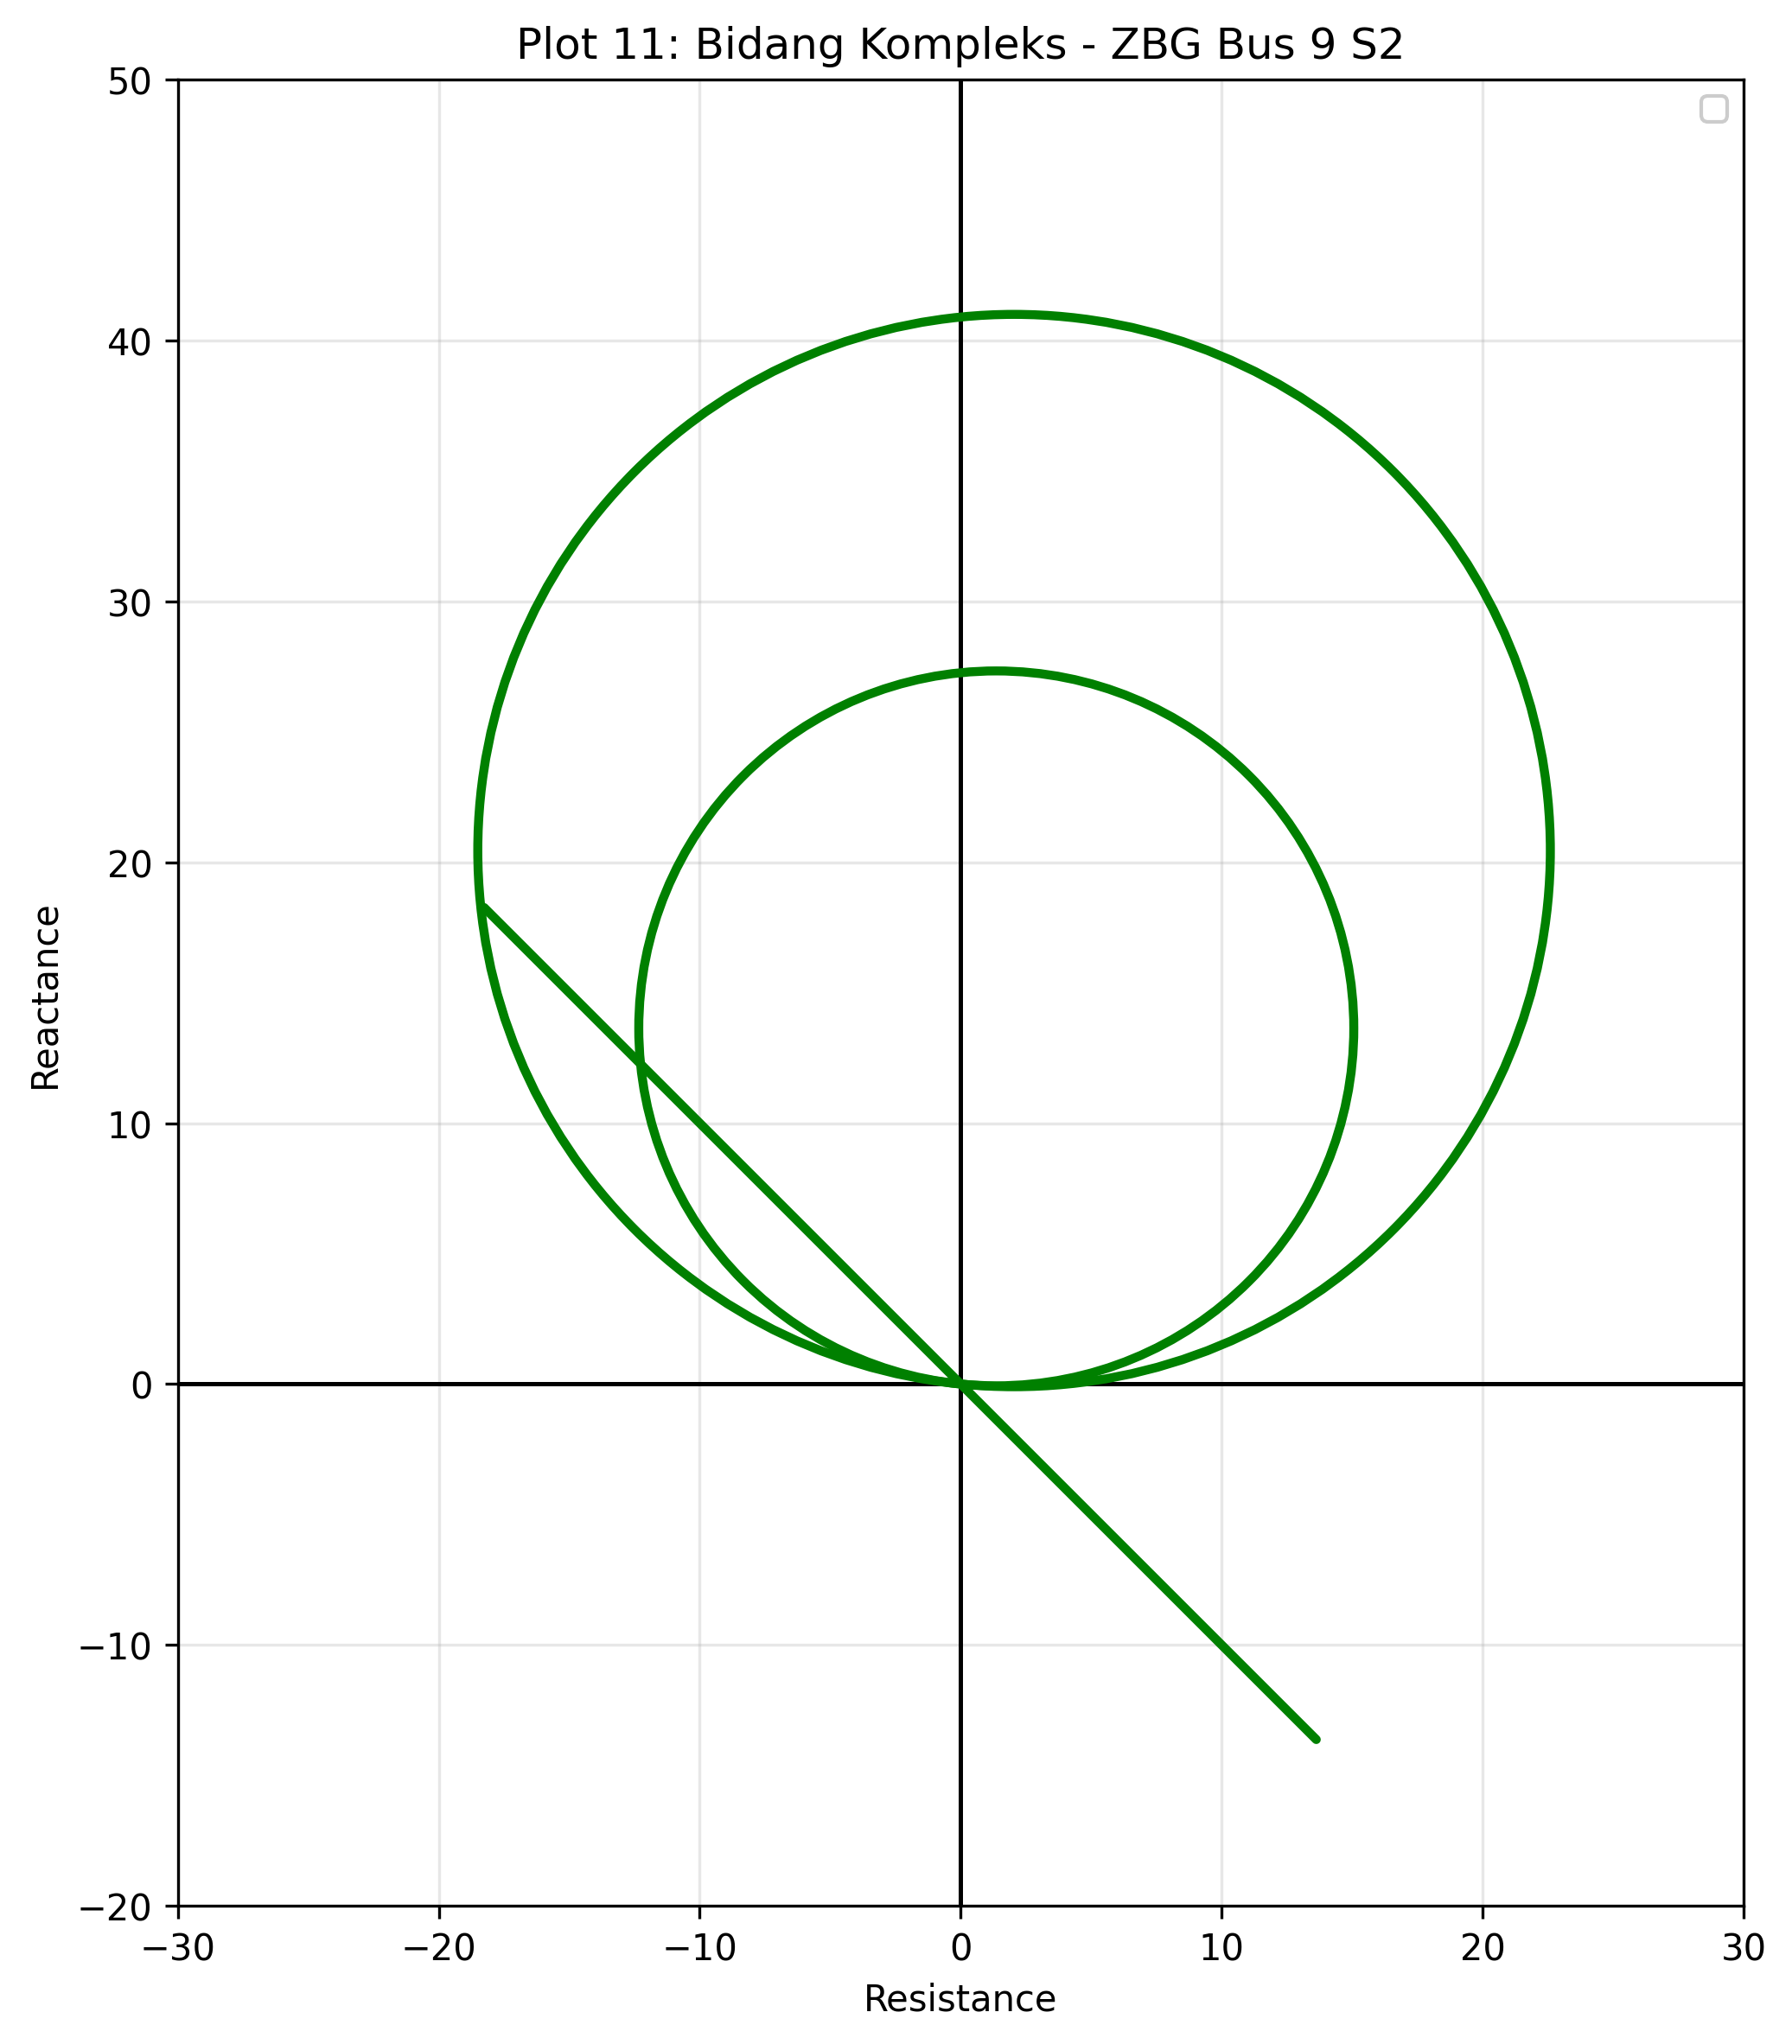
\includegraphics[width=\textwidth]{contents/chapter-4/PRIZI_11_ZBG_Bus_9_S2.png}
        \caption{Zoom In Pada Zona Proteksi}
        \label{fig:PRIZI_11_ZBG_Bus_9_S2}
    \end{subfigure}

    \caption{Impedansi Tampak ZBG Bus 9 Skenario 2}
    \label{fig:Impedansi_Tampak_ZBG_Bus_9_S2}
\end{figure}

Terlihat pada gambar \ref{fig:Impedansi_Tampak_ZBG_Bus_9_S2} bahwa impedansi tampak pada fasa B dengan ground yang dibaca oleh relay 21 sisi bus 9 saat terdapat gangguan bekerja dengan baik sesuai acuan pada \ref{subsec:tanpa_IBR_ex_dlg} relay 21 bus 9 tidak mendeteksi adanya gangguan sehingga tidak mengirimkan sinyal trip kepada CB.


%%%%%%%%%%%%%%%%%%%%%%%%%%%%%%%%%%%%%%%%%%%%%%%%%%%%%%%%%%%%%%

% \begin{figure}[H]
%     \centering
%     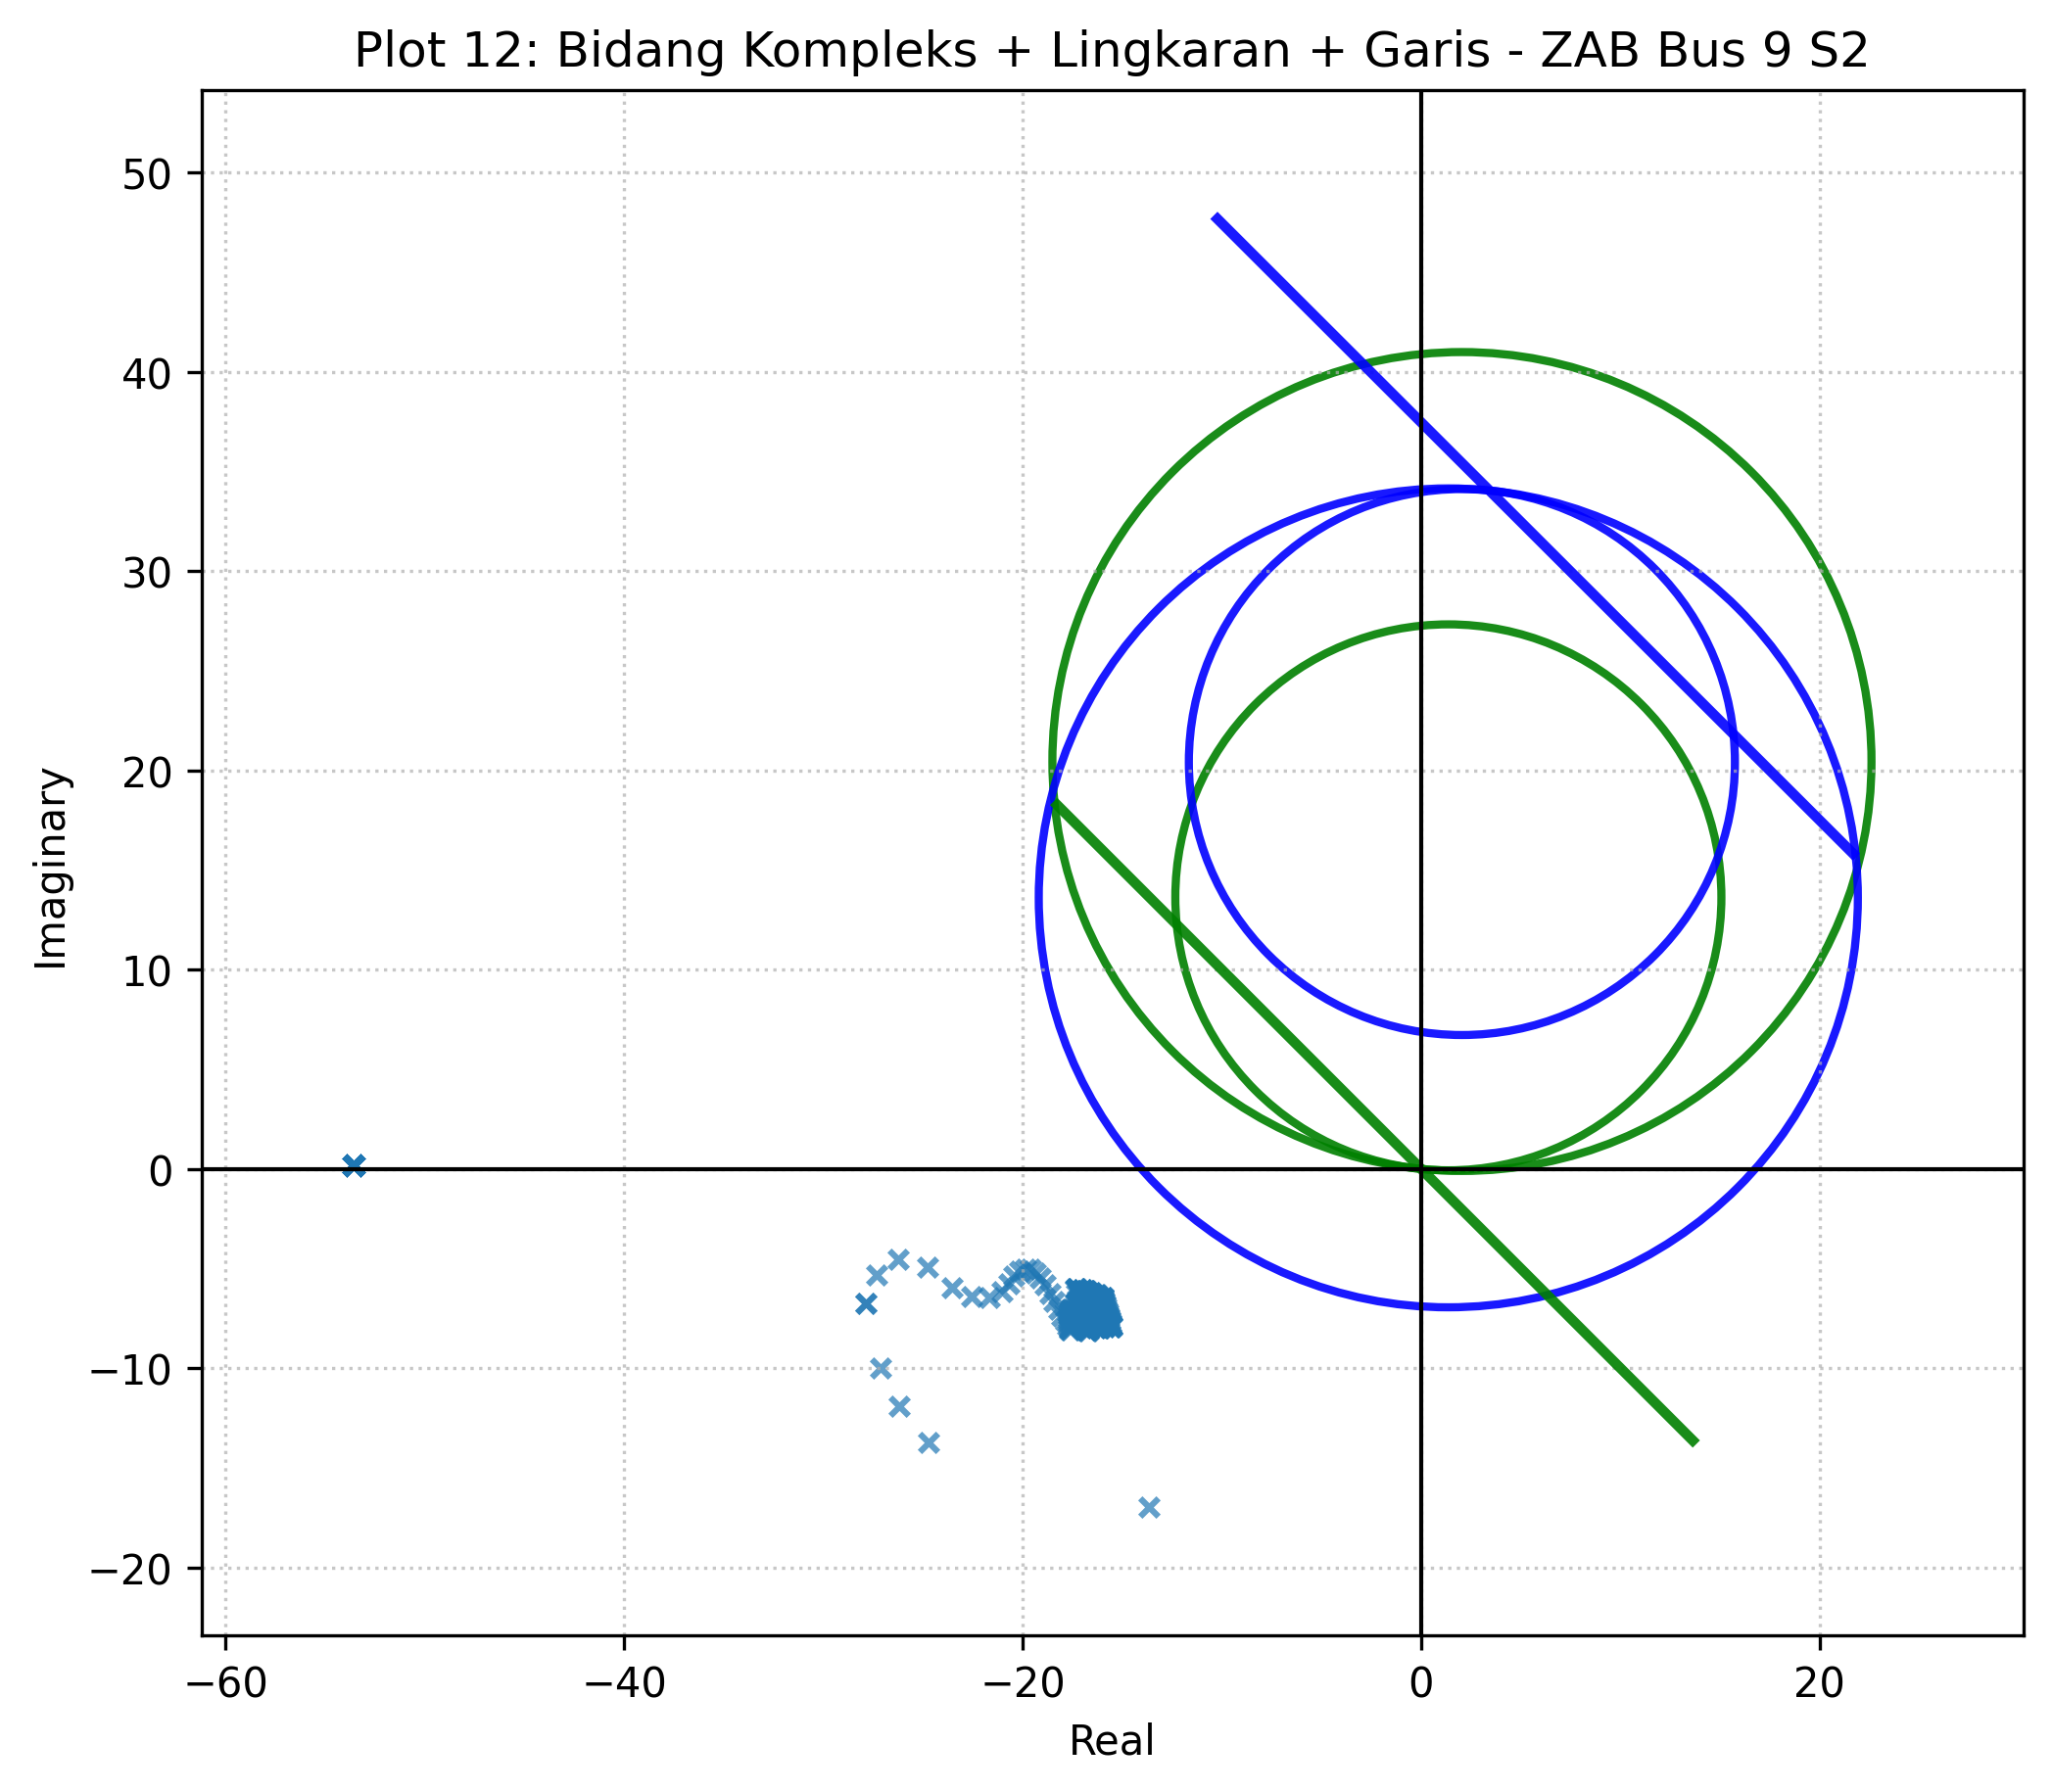
\includegraphics[width=0.8\textwidth]{contents/chapter-4/12_ZAB_Bus_9_S2_dengan_lingkaran_dan_garis.png}
%     \caption{Impedansi Tampak ZAB Bus 9 Skenario 2}
%     \label{fig:12_ZAB_Bus_9_S2_dengan_lingkaran_dan_garis}
% \end{figure}

% Terlihat pada gambar \ref{fig:11_ZBG_Bus_9_S2_dengan_lingkaran_dan_garis} bahwa impedansi tampak pada fasa A dengan fasa B yang dibaca oleh relay 21 sisi bus 9 saat terdapat gangguan external DLG bekerja dengan baik sesuai acuan pada \ref{subsec:tanpa_IBR_in_dlg} relay 21 bus 9 tidak mendeteksi adanya gangguan sehingga tidak mengirimkan sinyal trip kepada CB.

%%%%%%%%%%%%%%%%%%%%%%%%%%%%%%%%%SISI PRIMER%%%%%%%%%%%%%%%%%%%%%%%%%%%%%%%%%%

% \begin{figure}[H]
%     \centering
%     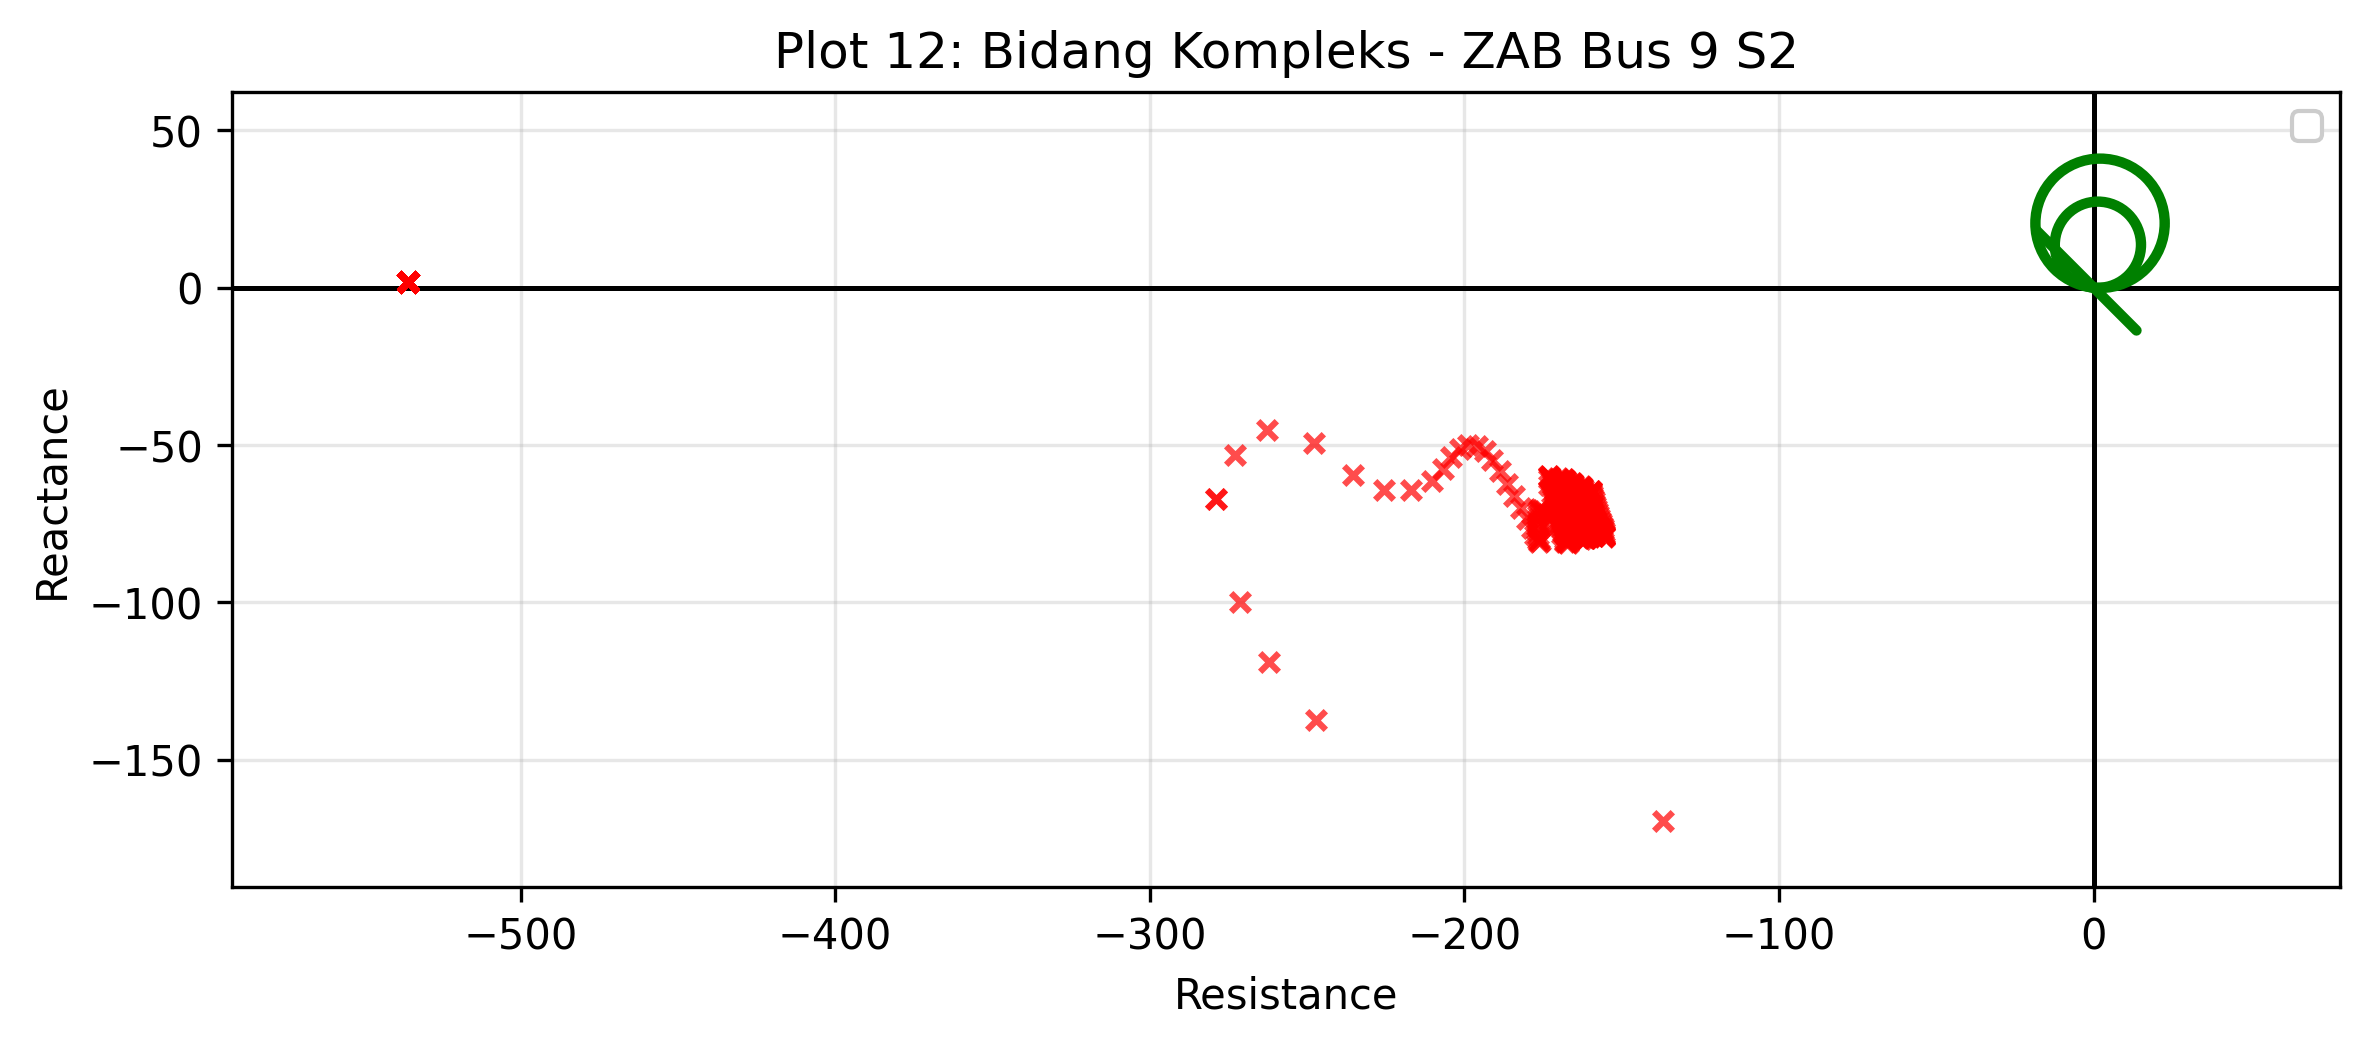
\includegraphics[width=0.8\textwidth]{contents/chapter-4/PRIA_12_ZAB_Bus_9_S2.png}
%     \caption{Impedansi Tampak ZAB Bus 9 Skenario 2}
%     \label{fig:PRIA_12_ZAB_Bus_9_S2}
% \end{figure}

% \begin{figure}[H]
%     \centering
%     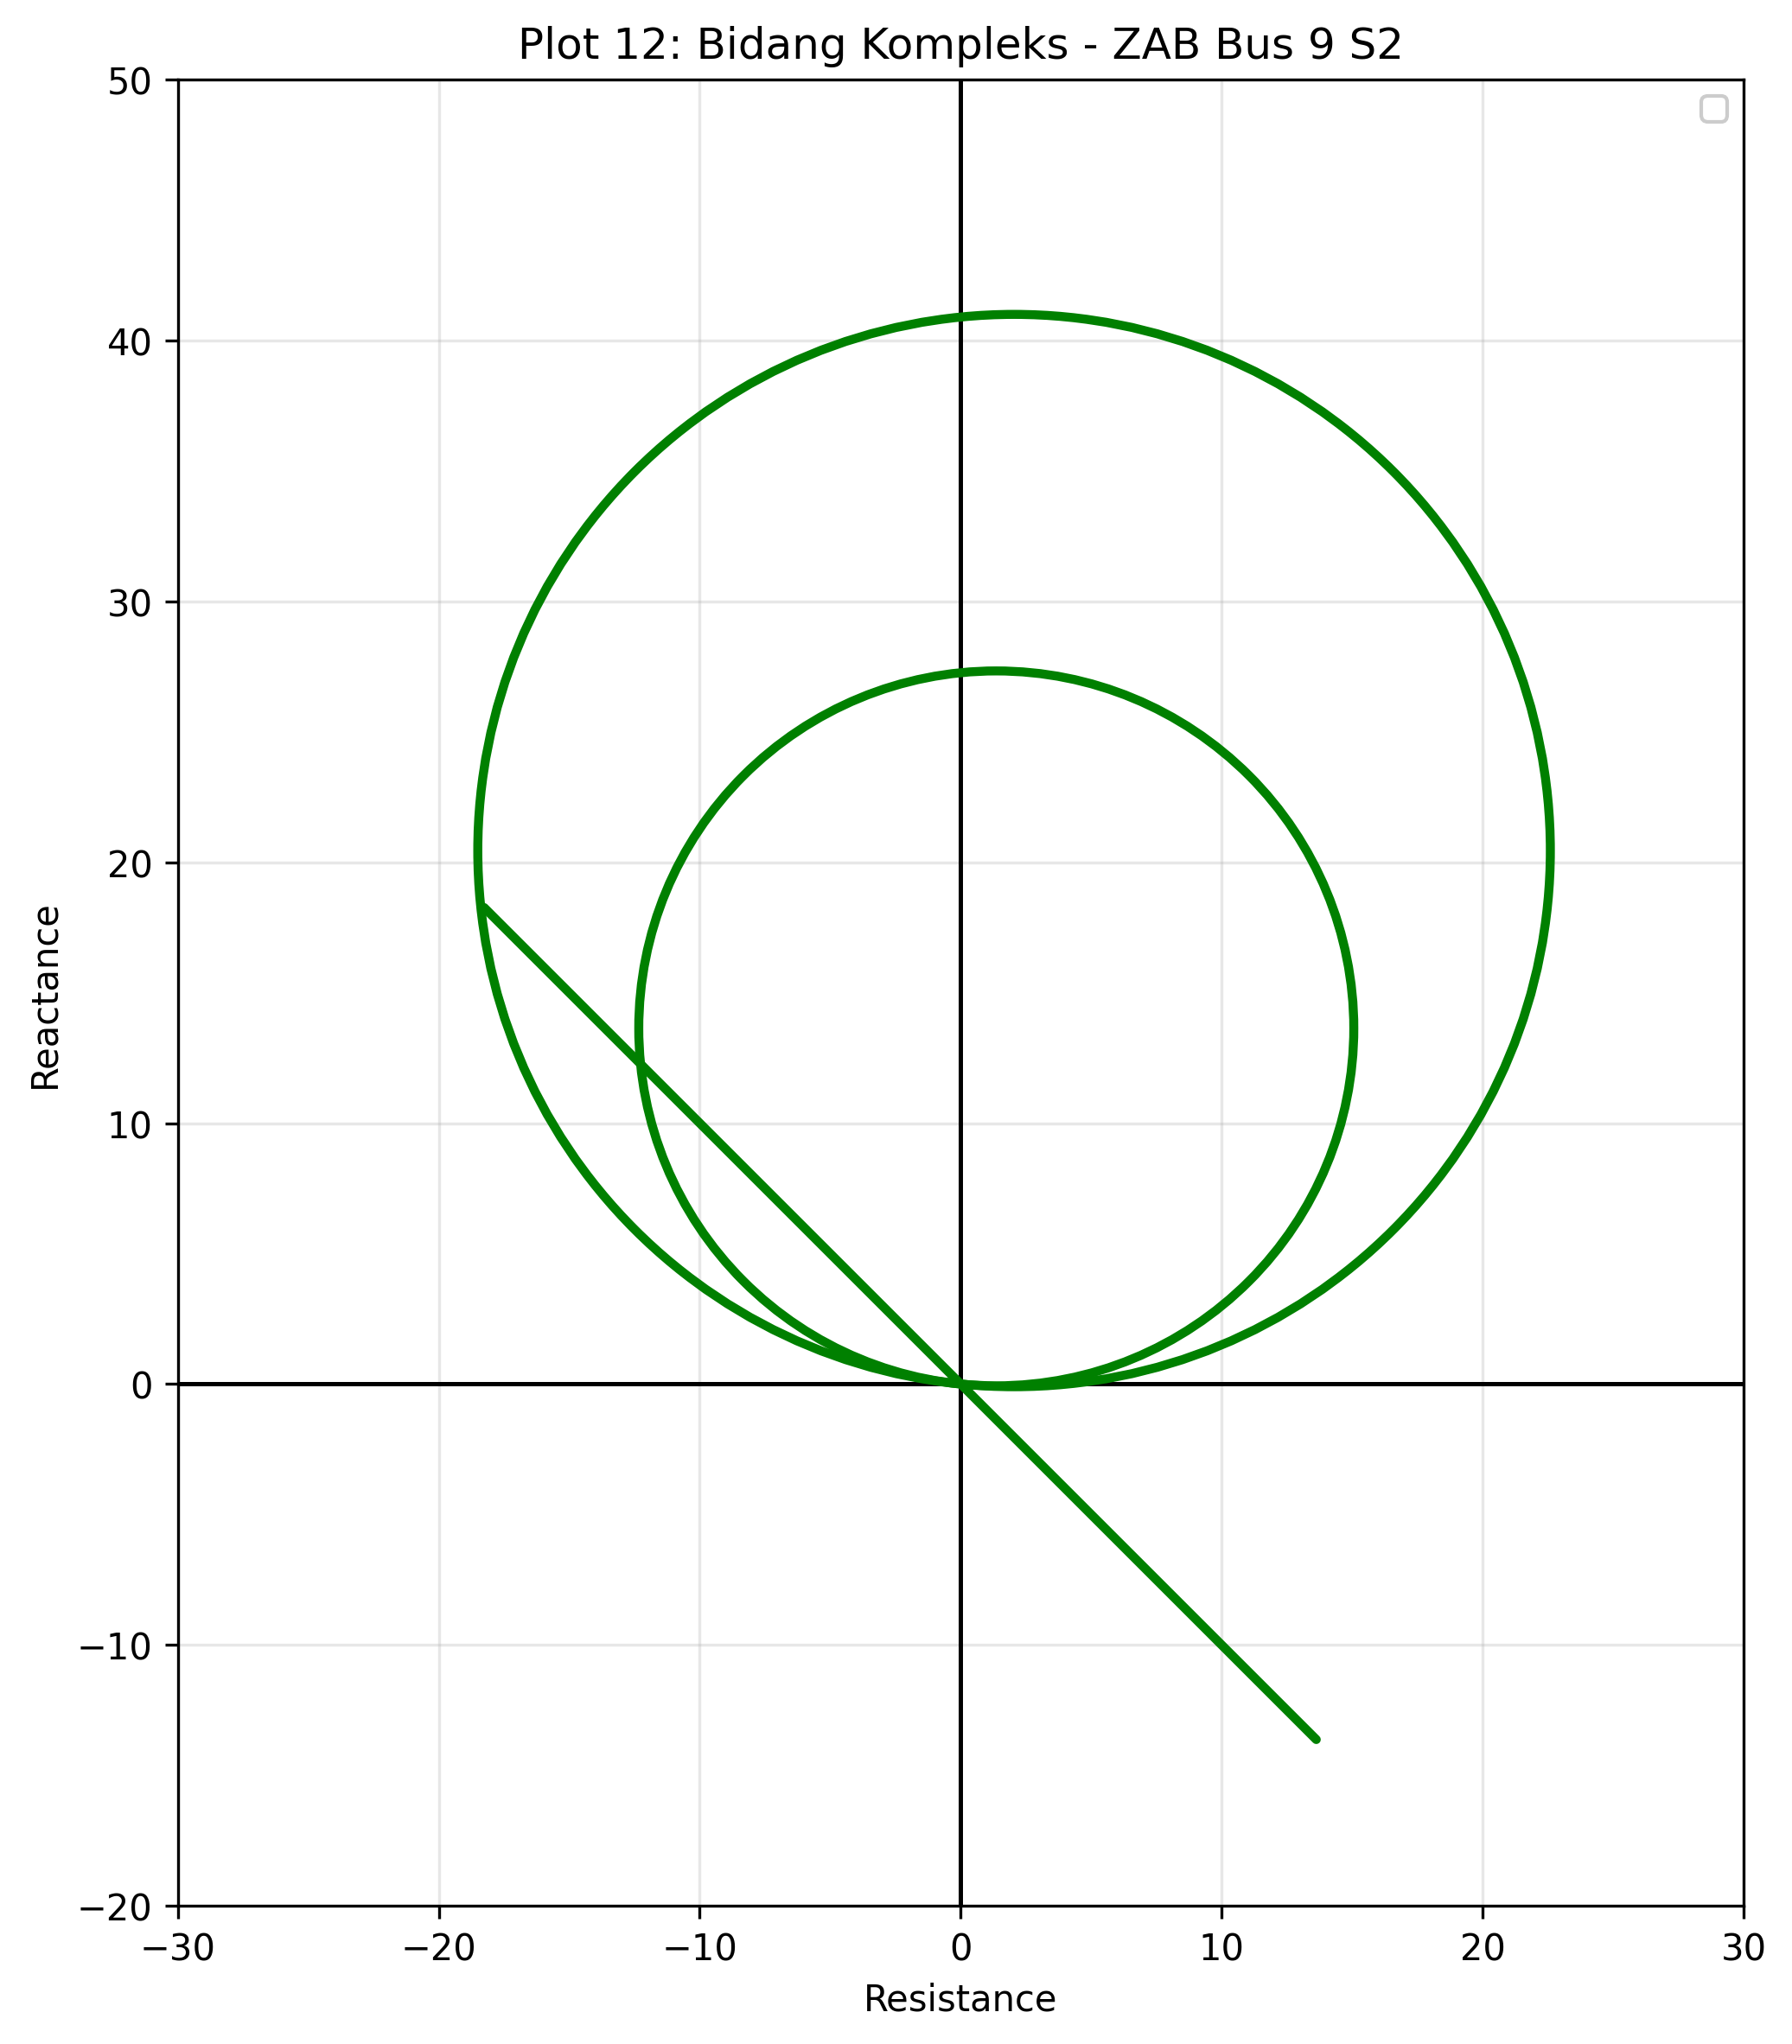
\includegraphics[width=0.8\textwidth]{contents/chapter-4/PRIZI_12_ZAB_Bus_9_S2.png}
%     \caption{Impedansi Tampak ZAB Bus 9 Skenario 2}
%     \label{fig:PRIZI_12_ZAB_Bus_9_S2}
% \end{figure}

\begin{figure}[H]
    \centering

    % Gambar sebelah kiri
    \begin{subfigure}[t]{0.48\textwidth}
        \centering
        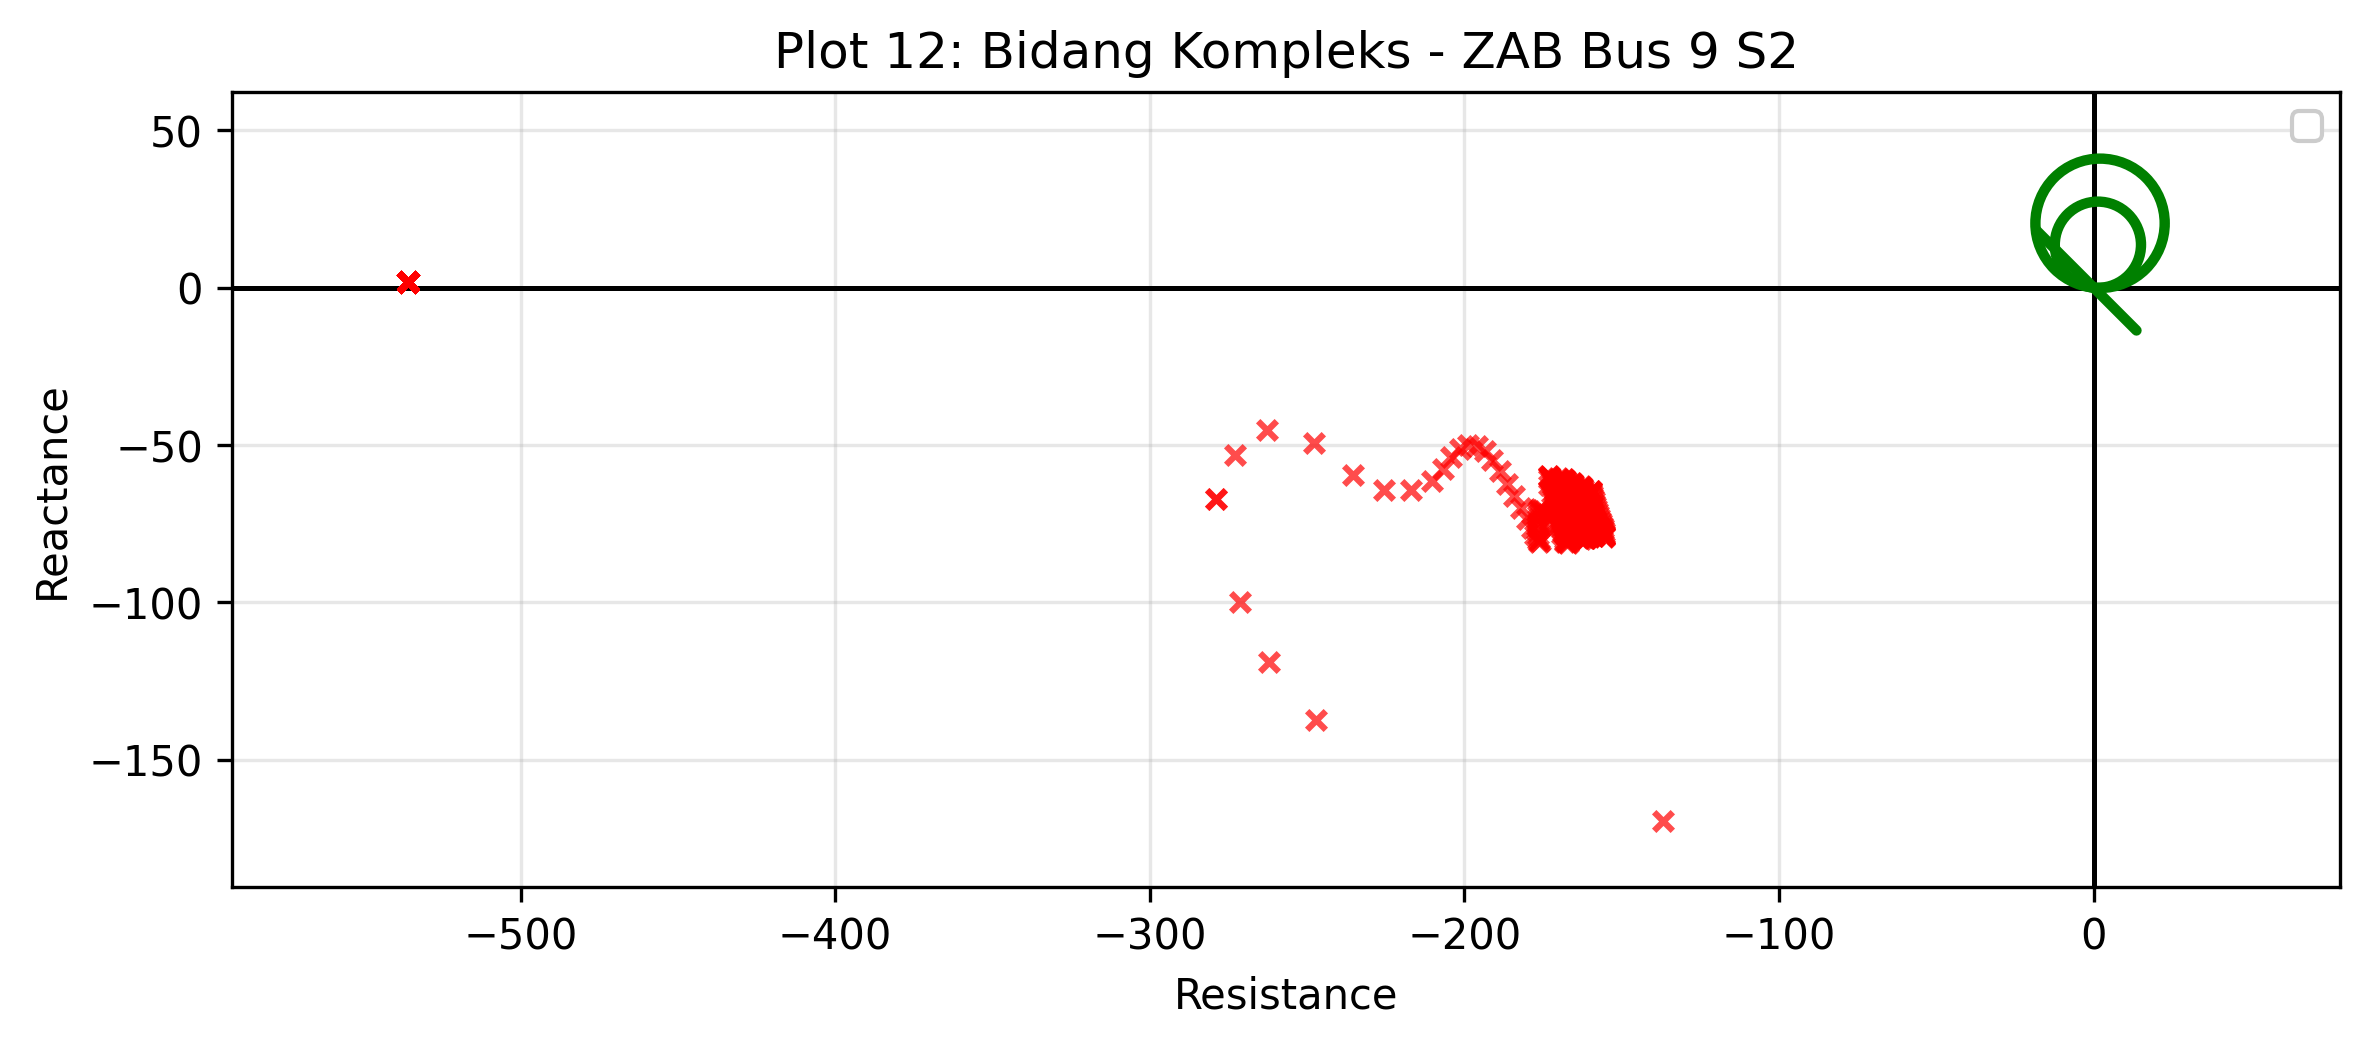
\includegraphics[width=\textwidth]{contents/chapter-4/PRIA_12_ZAB_Bus_9_S2.png}
        \caption{Seluruh Impedansi Tampak}
        \label{fig:PRIA_12_ZAB_Bus_9_S2}
    \end{subfigure}
    \hfill
    % Gambar sebelah kanan
    \begin{subfigure}[t]{0.48\textwidth}
        \centering
        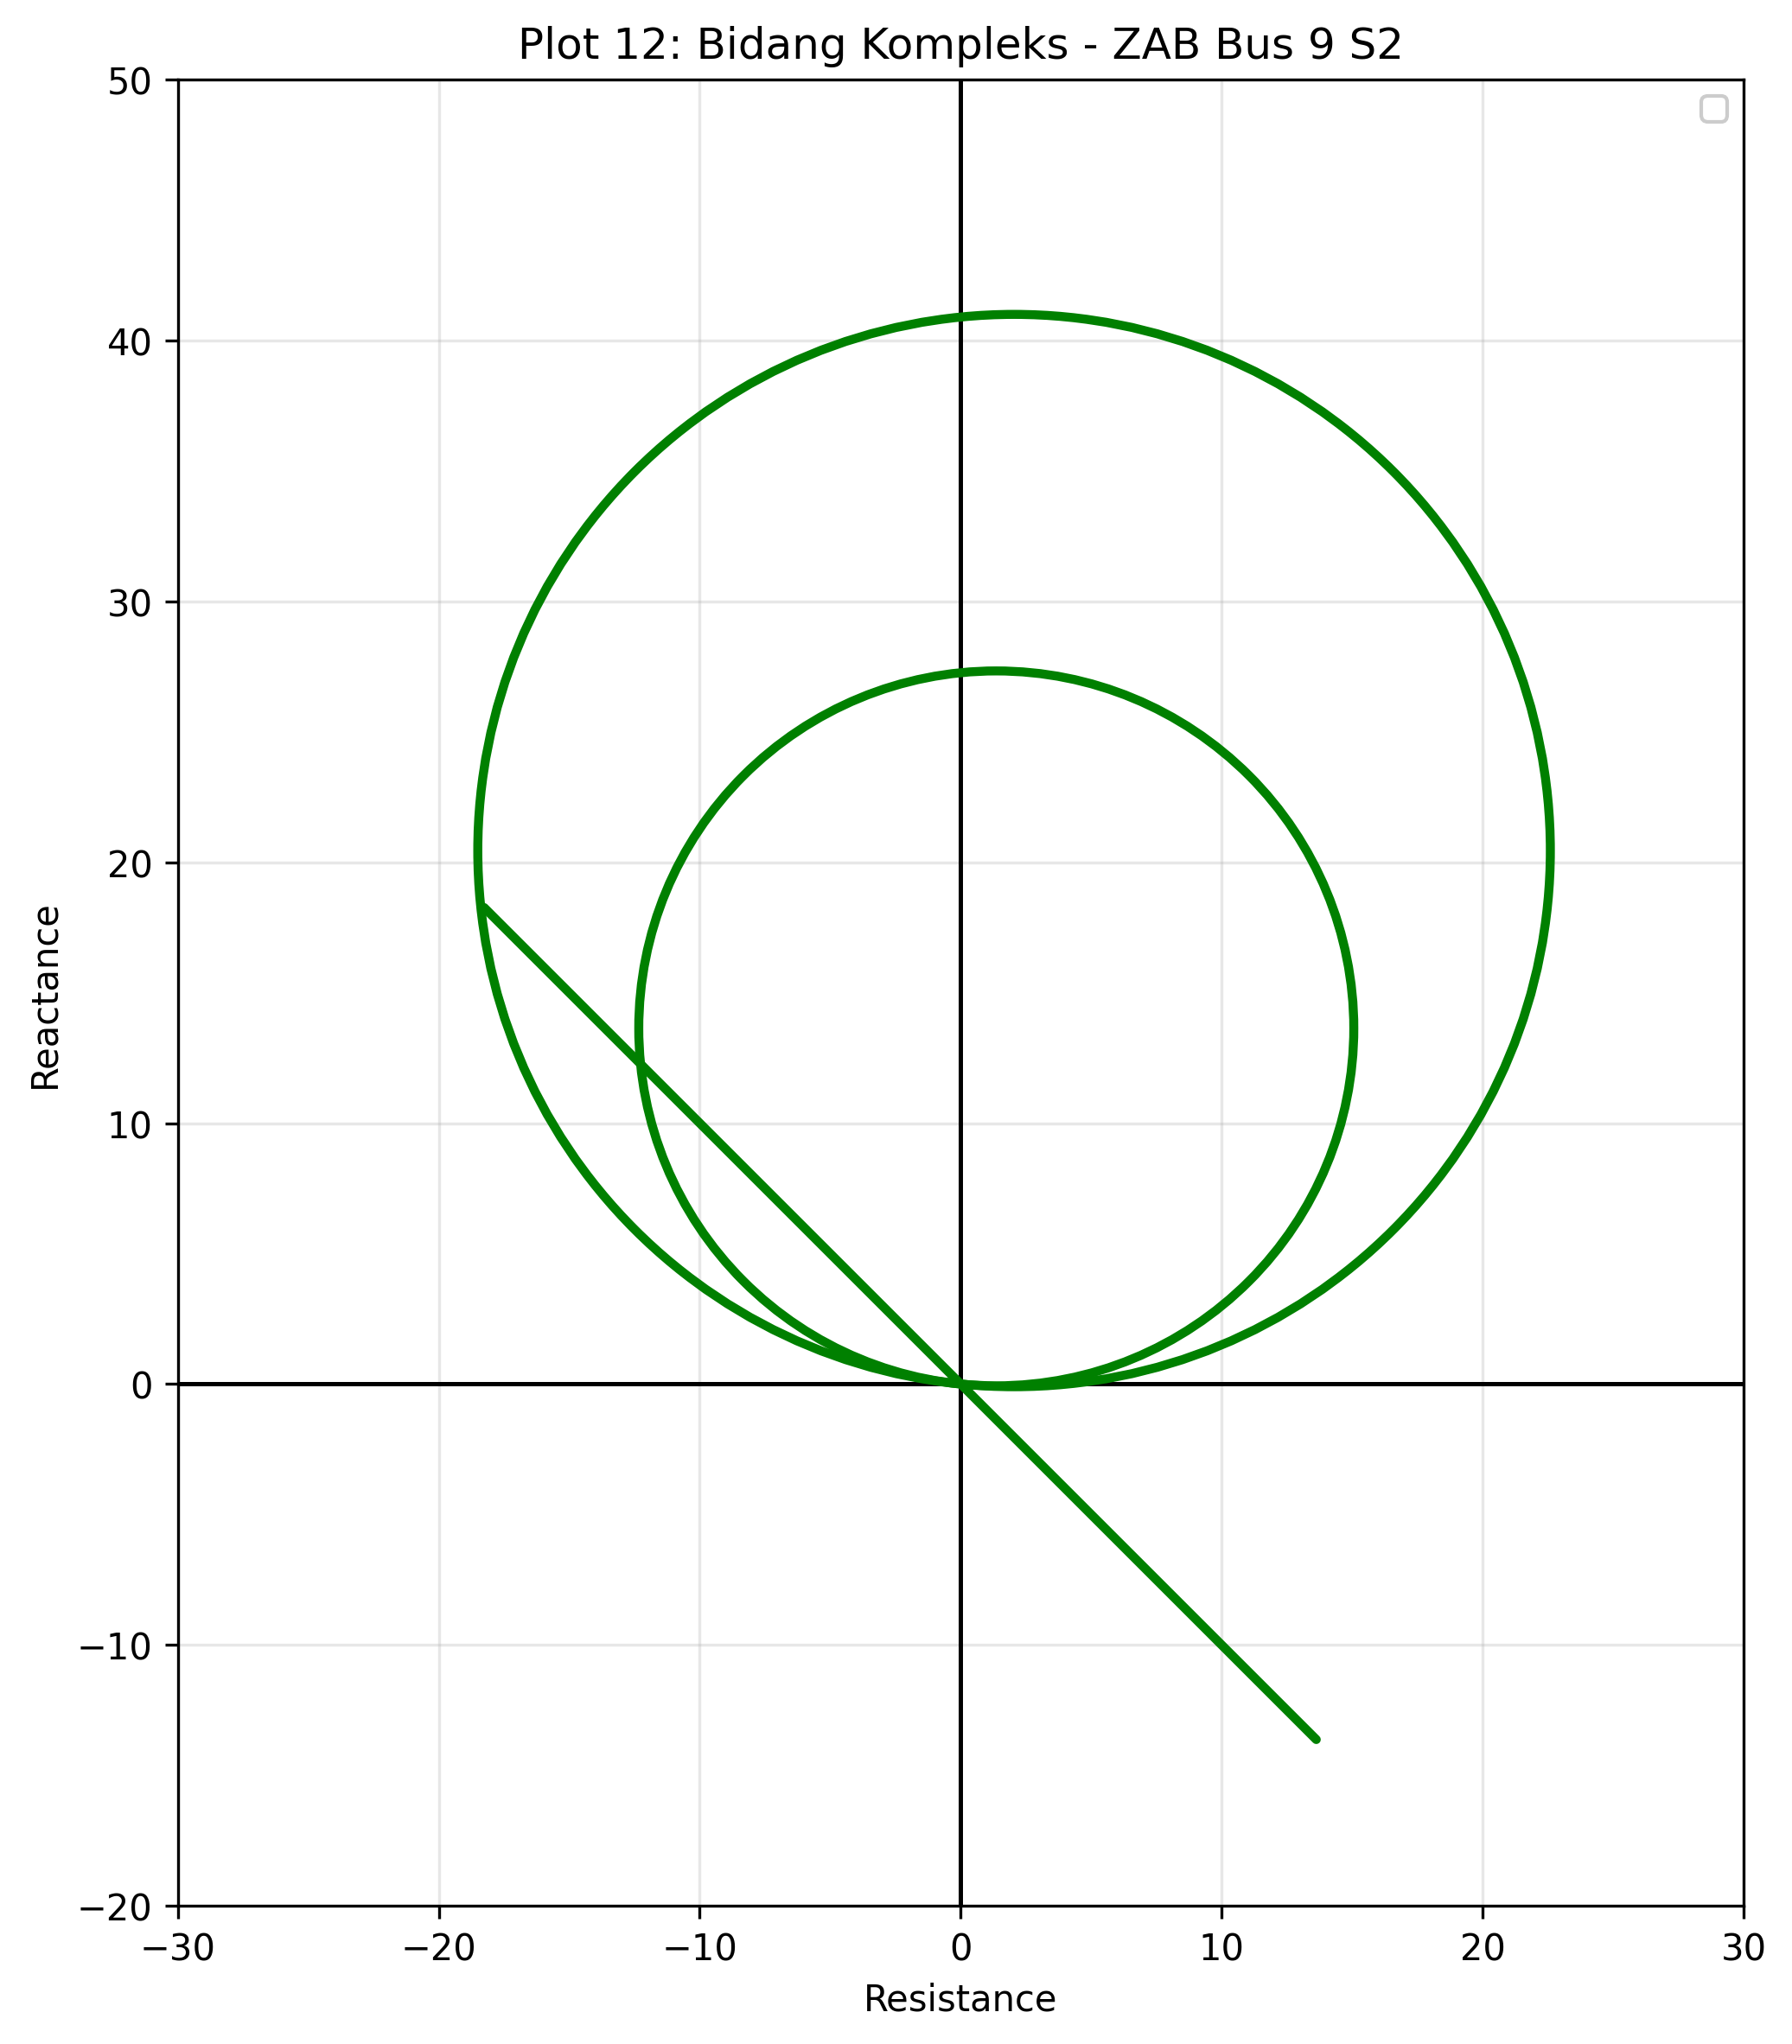
\includegraphics[width=\textwidth]{contents/chapter-4/PRIZI_12_ZAB_Bus_9_S2.png}
        \caption{Zoom In Pada Zona Proteksi}
        \label{fig:PRIZI_12_ZAB_Bus_9_S2}
    \end{subfigure}

    \caption{Impedansi Tampak ZAB Bus 9 Skenario 2}
    \label{fig:Impedansi_Tampak_ZAB_Bus_9_S2}
\end{figure}

Terlihat pada gambar \ref{fig:Impedansi_Tampak_ZAB_Bus_9_S2} bahwa impedansi tampak pada fasa B dengan ground yang dibaca oleh relay 21 sisi bus 9 saat terdapat gangguan bekerja dengan baik sesuai acuan pada \ref{subsec:tanpa_IBR_ex_dlg} relay 21 bus 9 tidak mendeteksi adanya gangguan sehingga tidak mengirimkan sinyal trip kepada CB.


%%%%%%%%%%%%%%%%%%%%%%%%%%%%%%%%%%%%%%%%%%%%%%%%%%%%%%%%%%%%%%

% pada gambar \ref{fig:10_ZAG_Bus_9_S2_dengan_lingkaran_dan_garis.png} hingga \ref{fig:12_ZAB_Bus_9_S2_dengan_lingkaran_dan_garis.png} terlihat bahwa impedansi tampak yang dibaca oleh relay 21 dari sisi bus 9 berada pada luar zona yang di tentukan namun relay mengalmi misoperation dimana seharusnya tidak trip namun menjadi trip.



\section{Respons Relay 21 pada Sistem dengan Photovoltaic}

Bagian ini membahas respons relay 21 ketika sumber IBR yang digunakan adalah \textit{photovoltaic}. Skenario yang diamati adalah gangguan eksternal DLG pada TL79 dengan TL78 \textit{out of service}. Dengan struktur yang sama seperti bagian \textit{wind turbine type 4}, pembahasan diarahkan untuk melihat apakah karakteristik PV menghasilkan perubahan pada impedansi tampak dan keputusan operasi relay 21.

Hasil pada sisi Bus 8 dan Bus 9 kembali dibandingkan terhadap kondisi dasar gangguan eksternal DLG. Perbandingan ini penting karena pada skenario eksternal, relay diharapkan hanya bekerja sesuai daerah dan arah proteksinya, sedangkan perubahan kontribusi arus dari IBR dapat memengaruhi kondisi \textit{starting} maupun posisi titik impedansi tampak.

\subsection{Skenario 6 : Photovoltaic External DLG Fault}

Skenario ini membahas respons relay 21 ketika jenis IBR yang digunakan adalah \textit{photovoltaic}. Gangguan yang diterapkan tetap berupa gangguan eksternal DLG pada TL79 dengan TL78 \textit{out of service}, sehingga hasilnya dapat dibandingkan langsung dengan skenario eksternal DLG lain yang telah dibahas sebelumnya.

Hasil dekomposisi komponen urutan arus pada Gambar \ref{fig:decomposition_sequence_current_s6} digunakan sebagai dasar untuk membaca hubungan antara karakter arus pada sistem dengan PV dan pembacaan relay pada saluran TL89. Setelah konteks arus tersebut ditetapkan, analisis dilanjutkan pada impedansi tampak elemen ZAG, ZBG, dan ZAB dari sisi Bus 8 serta Bus 9 untuk menilai apakah relay 21 tetap mengikuti acuan gangguan eksternal atau menunjukkan perubahan respons.

% \begin{figure}[H]
%     \centering
%     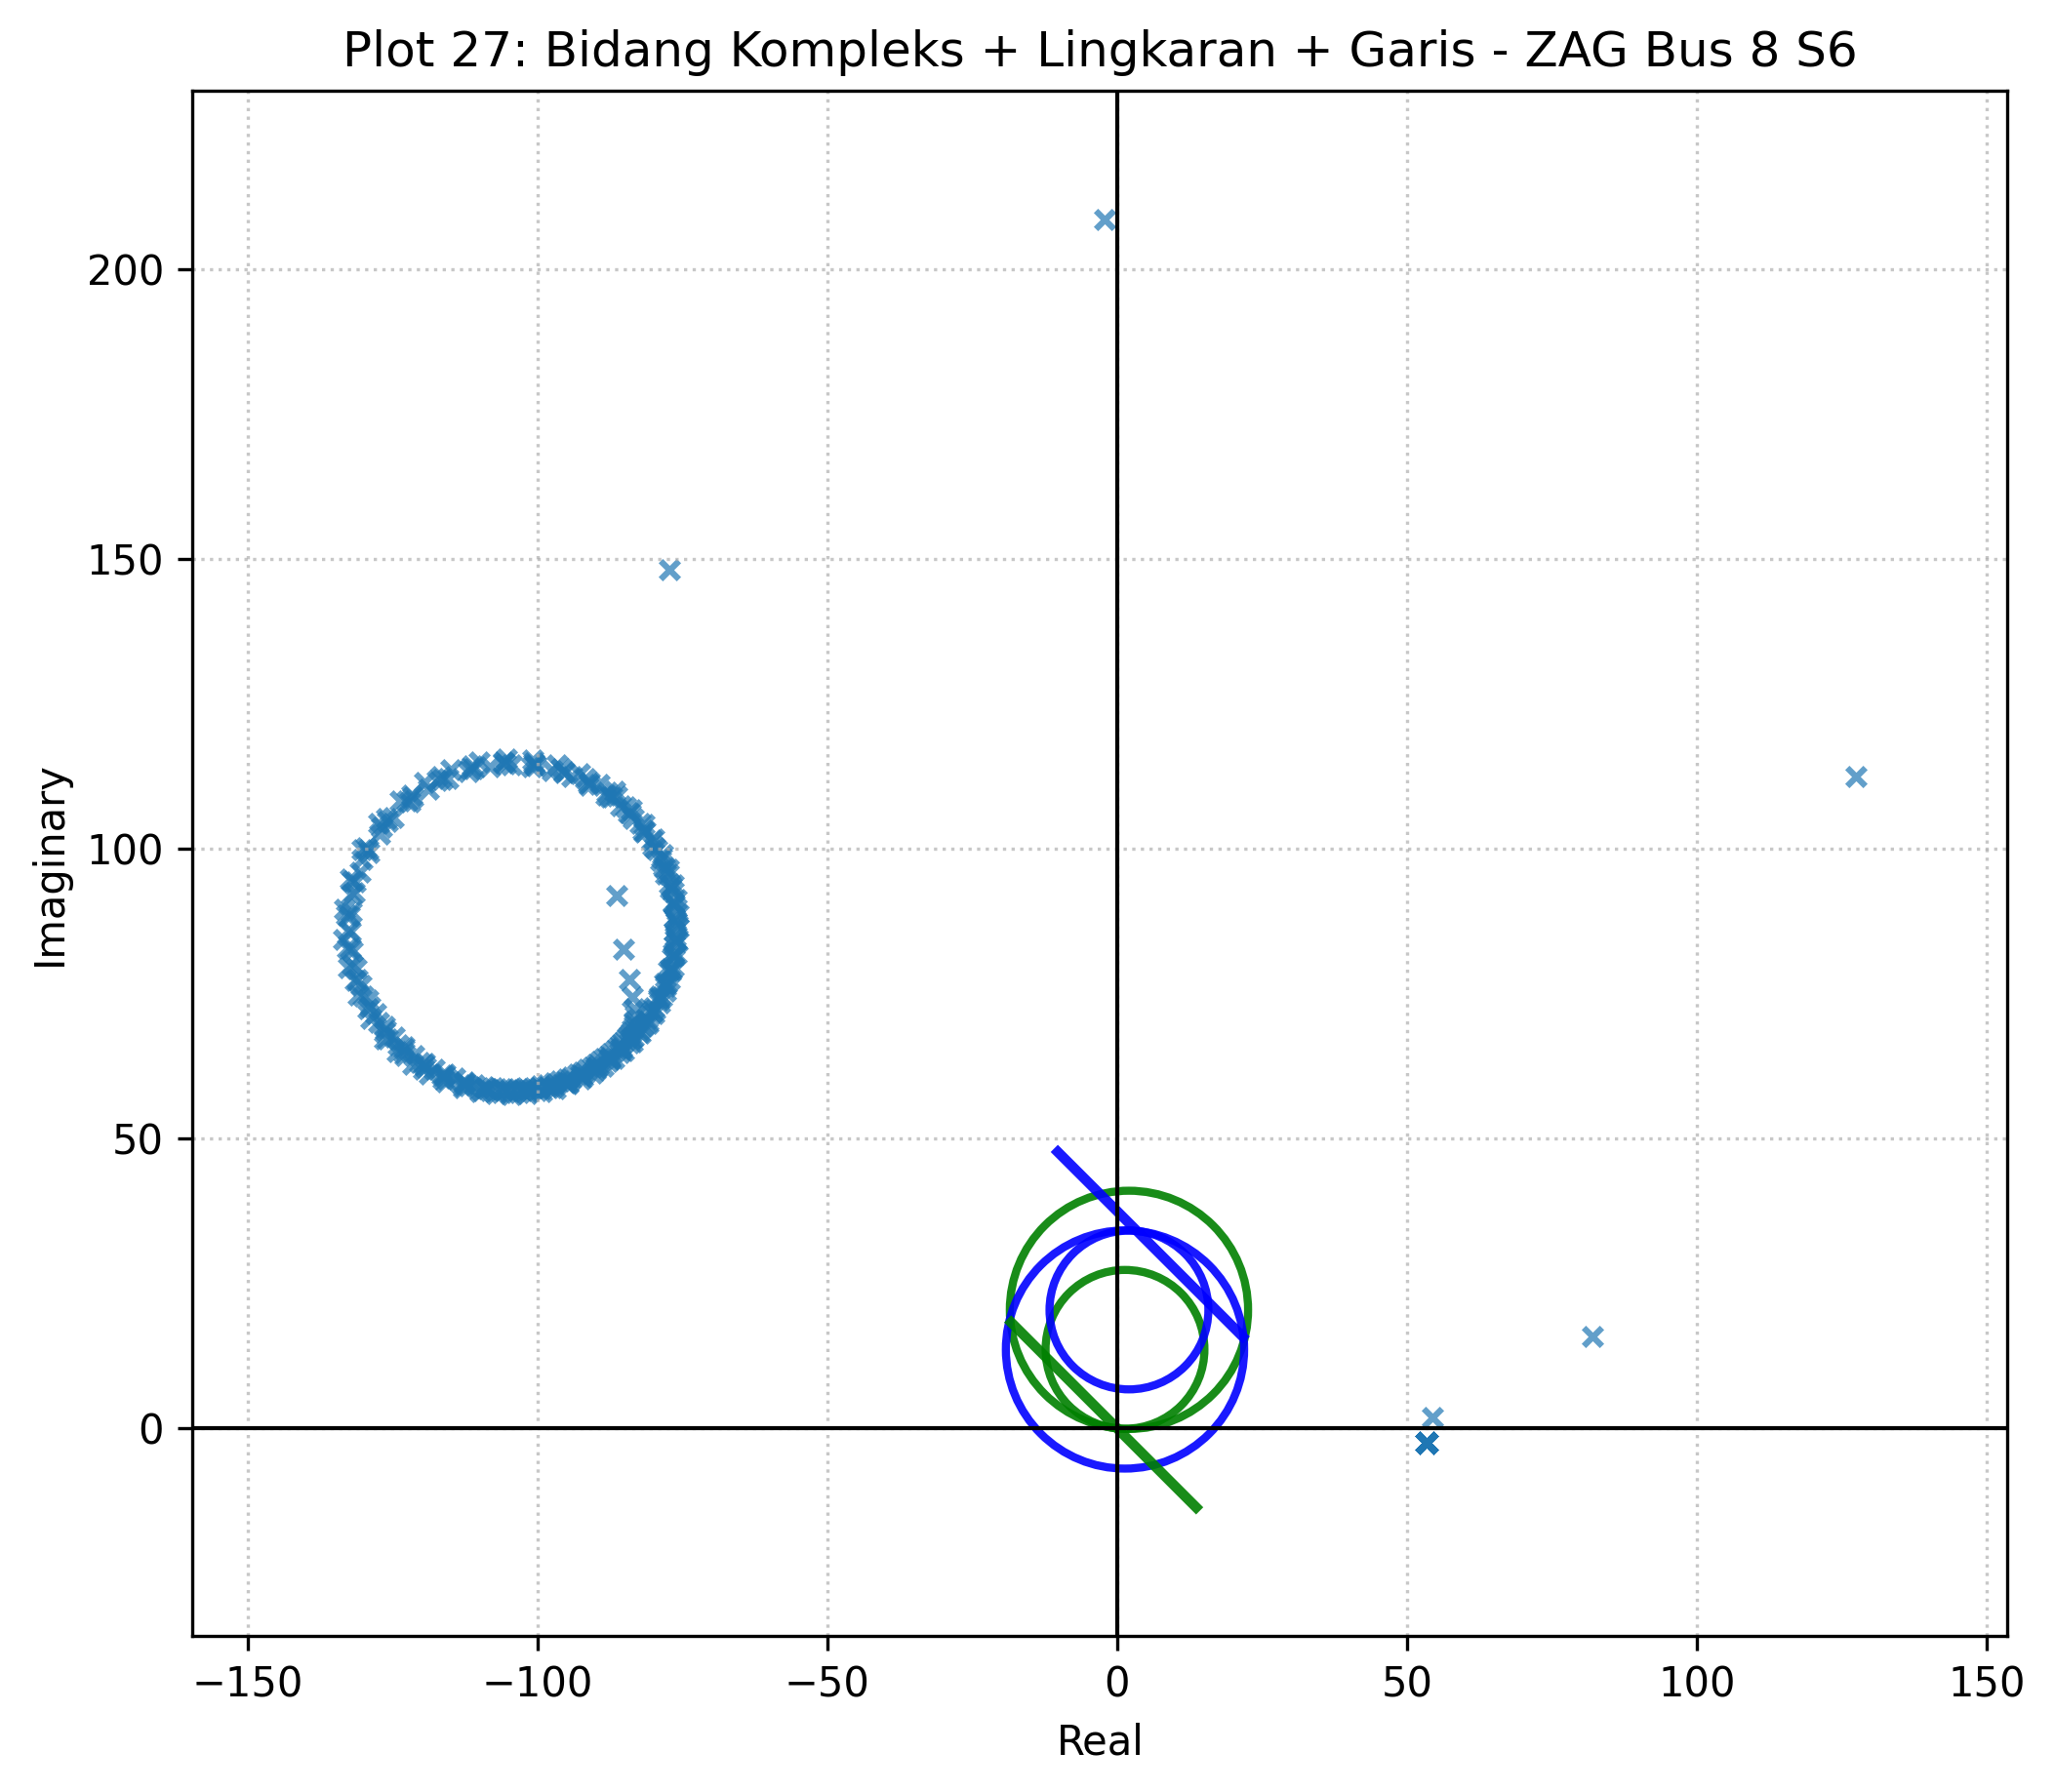
\includegraphics[width=0.8\textwidth]{contents/chapter-4/27_ZAG_Bus_8_S6_dengan_lingkaran_dan_garis.png}
%     \caption{Impedansi Tampak ZAG Bus 8 Skenario 6}
%     \label{fig:27_ZAG_Bus_8_S6_dengan_lingkaran_dan_garis}
% \end{figure}

% Terlihat pada gambar \ref{fig:27_ZAG_Bus_8_S6_dengan_lingkaran_dan_garis} bahwa impedansi tampak pada fasa A dengan ground yang dibaca oleh relay 21 sisi bus 8 saat terdapat gangguan external DLG bekerja dengan acuan pada \ref{subsec:tanpa_IBR_in_dlg} relay 21 bus 8 mengalami misoperation karena mendeteksi adanya gangguan namun overreach pada zona 1 yang seharusnya pada zona 2 serta mengalami dropout pada zona 2 dan memberikan sinyal trip kepada CB pada zona 2

%%%%%%%%%%%%%%%%%%%%%%%%%%%%%%%%%SISI PRIMER%%%%%%%%%%%%%%%%%%%%%%%%%%%%%%%%%%

\begin{figure}[H]
    \centering
    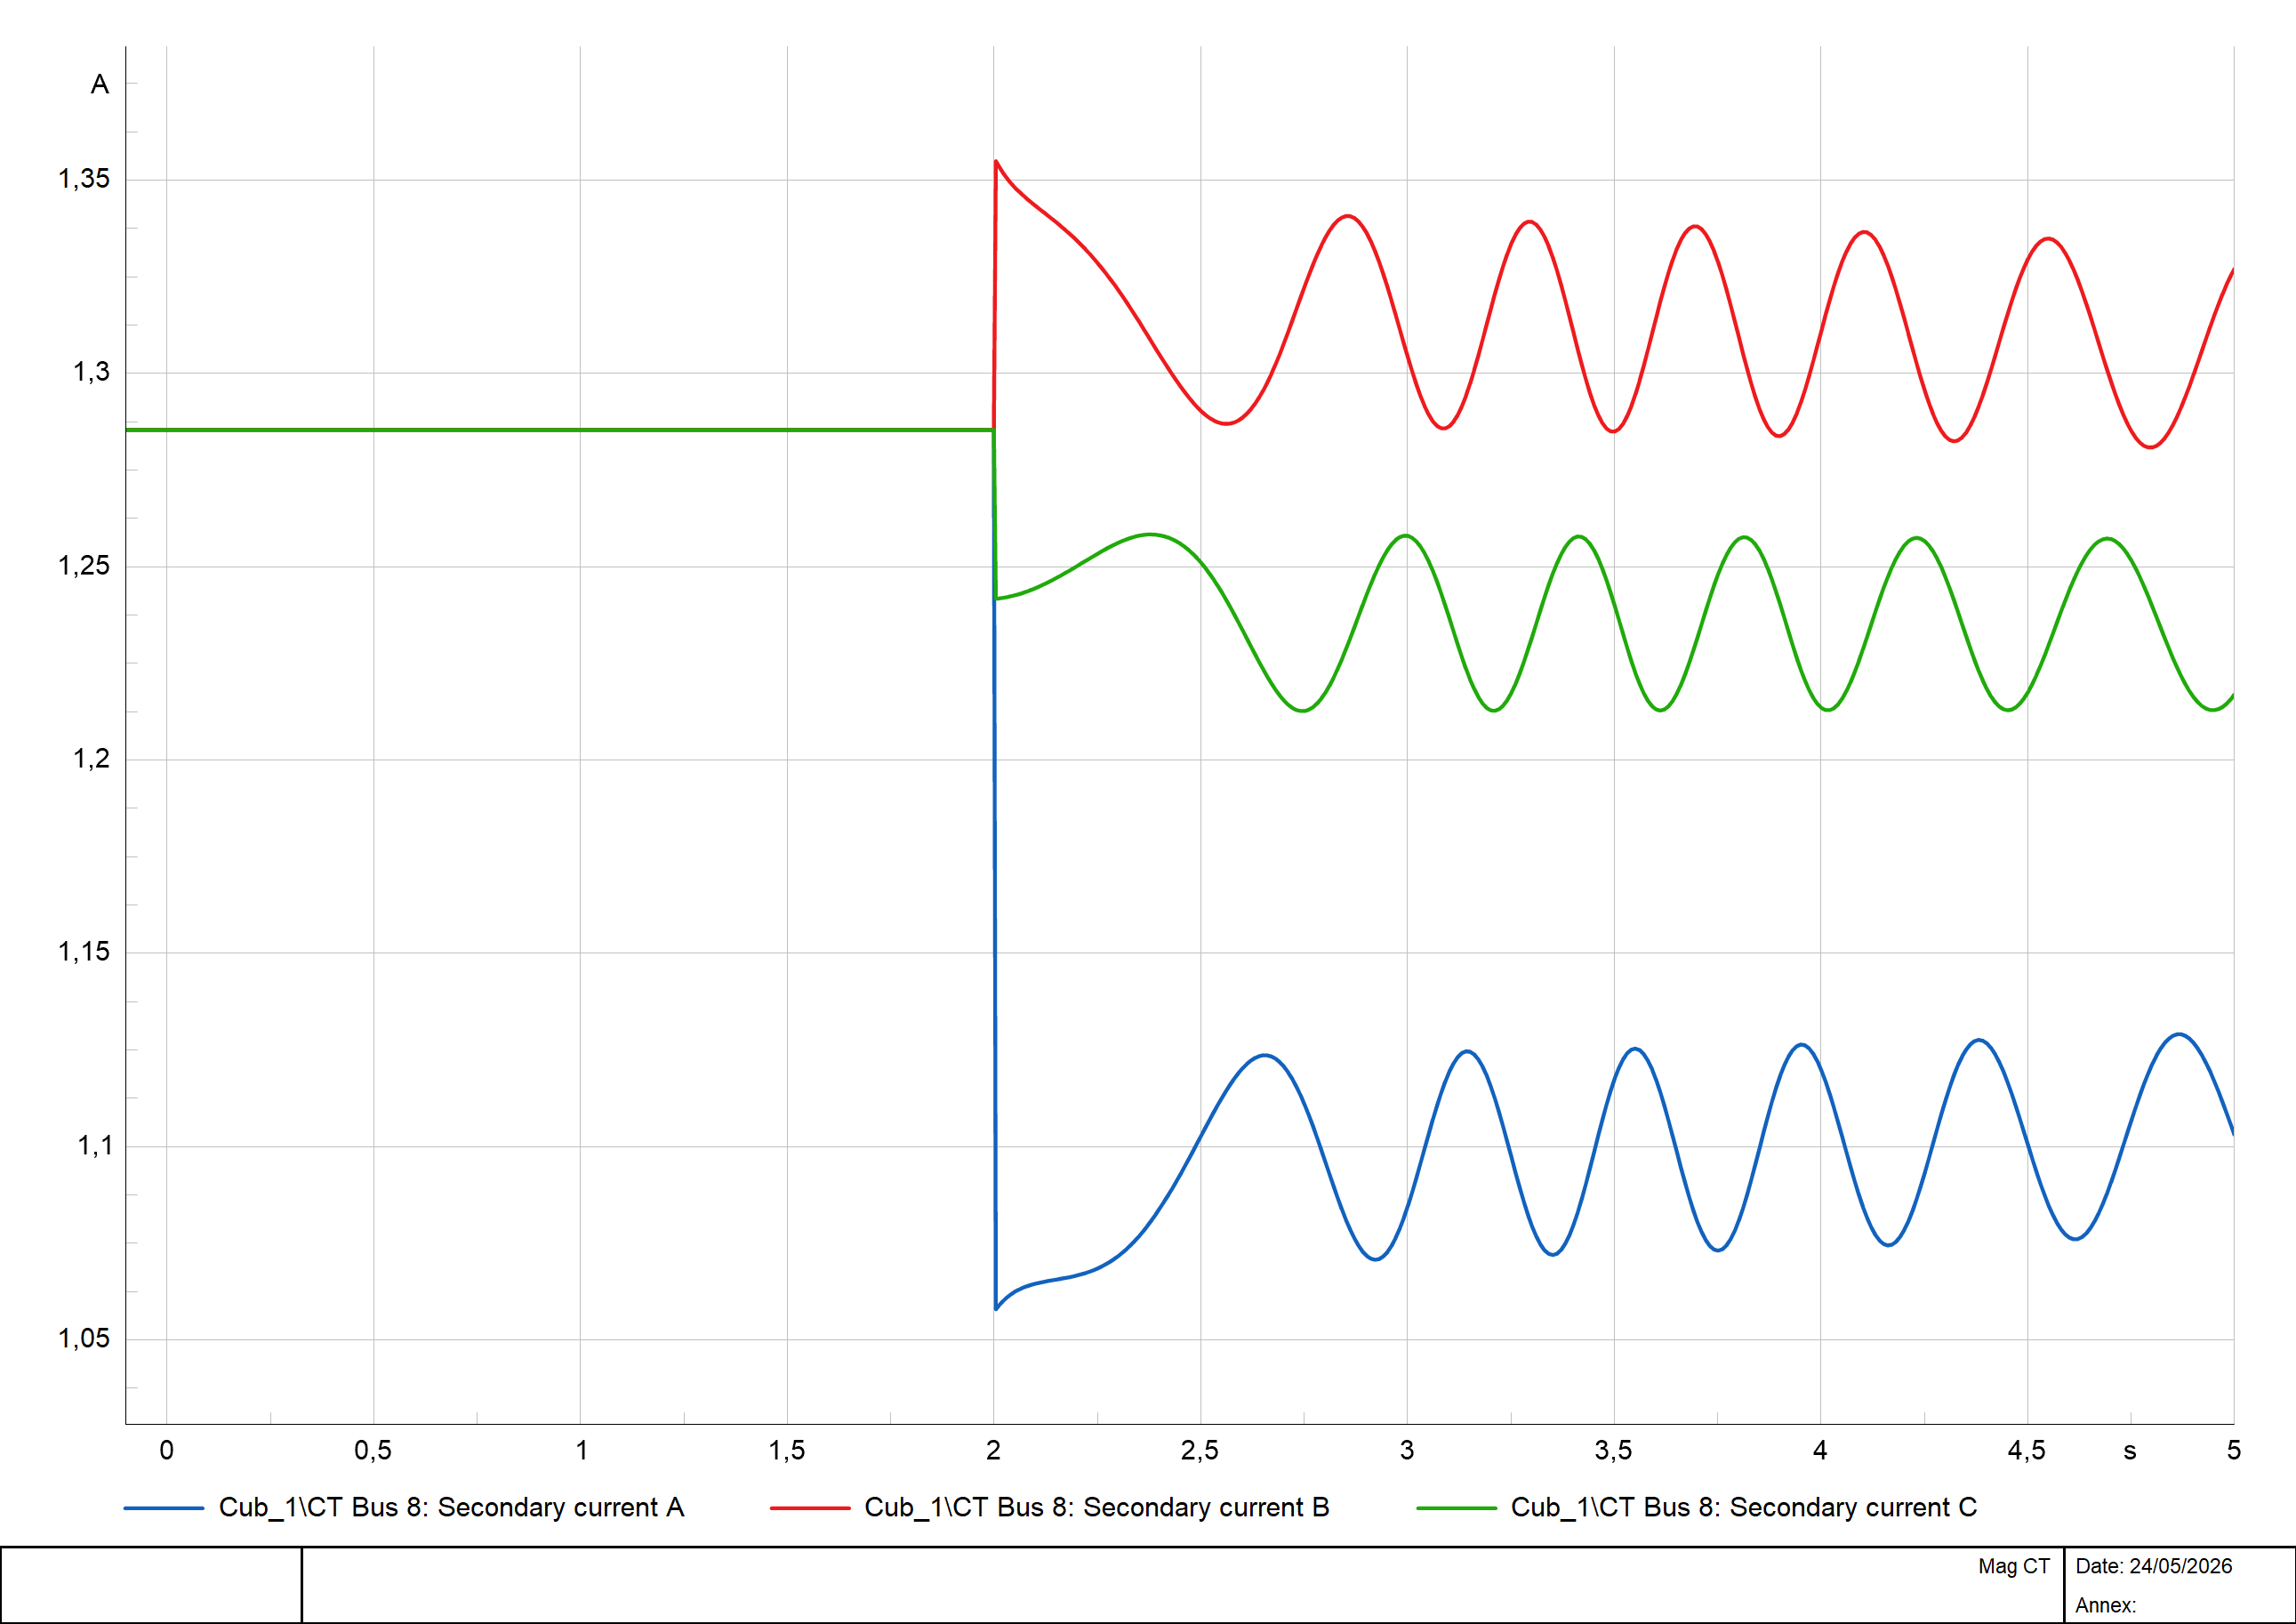
\includegraphics[width=0.8\textwidth]{contents/chapter-4/Bus_8_Ex_DLG_S6.png}
    \caption{Arus Sekunder CT Bus 8 Skenario 6}
    \label{fig:Bus_8_Ex_DLG_S6}
\end{figure}

Gambar \ref{fig:Bus_8_Ex_DLG_S6} menunjukkan arus sekunder CT pada Bus 8 untuk skenario 6 saat terjadi gangguan eksternal DLG. Sebelum gangguan, arus pada ketiga fasa berada pada nilai 1,285 A sekunder. Setelah gangguan terjadi, arus fasa A menurun menjadi 1,129 A sekunder atau 0,88 p.u., arus fasa B meningkat menjadi 1,355 A sekunder atau 1,05 p.u., dan arus fasa C menurun menjadi 1,258 A sekunder atau 0,98 p.u. Perubahan arus tersebut menunjukkan adanya respons saat gangguan, tetapi nilainya masih belum memenuhi arus minimum yang diperlukan untuk membuat relay 21 sisi Bus 8 aktif.

\begin{figure}[H]
    \centering

    % Gambar sebelah kiri
    \begin{subfigure}[t]{0.48\textwidth}
        \centering
        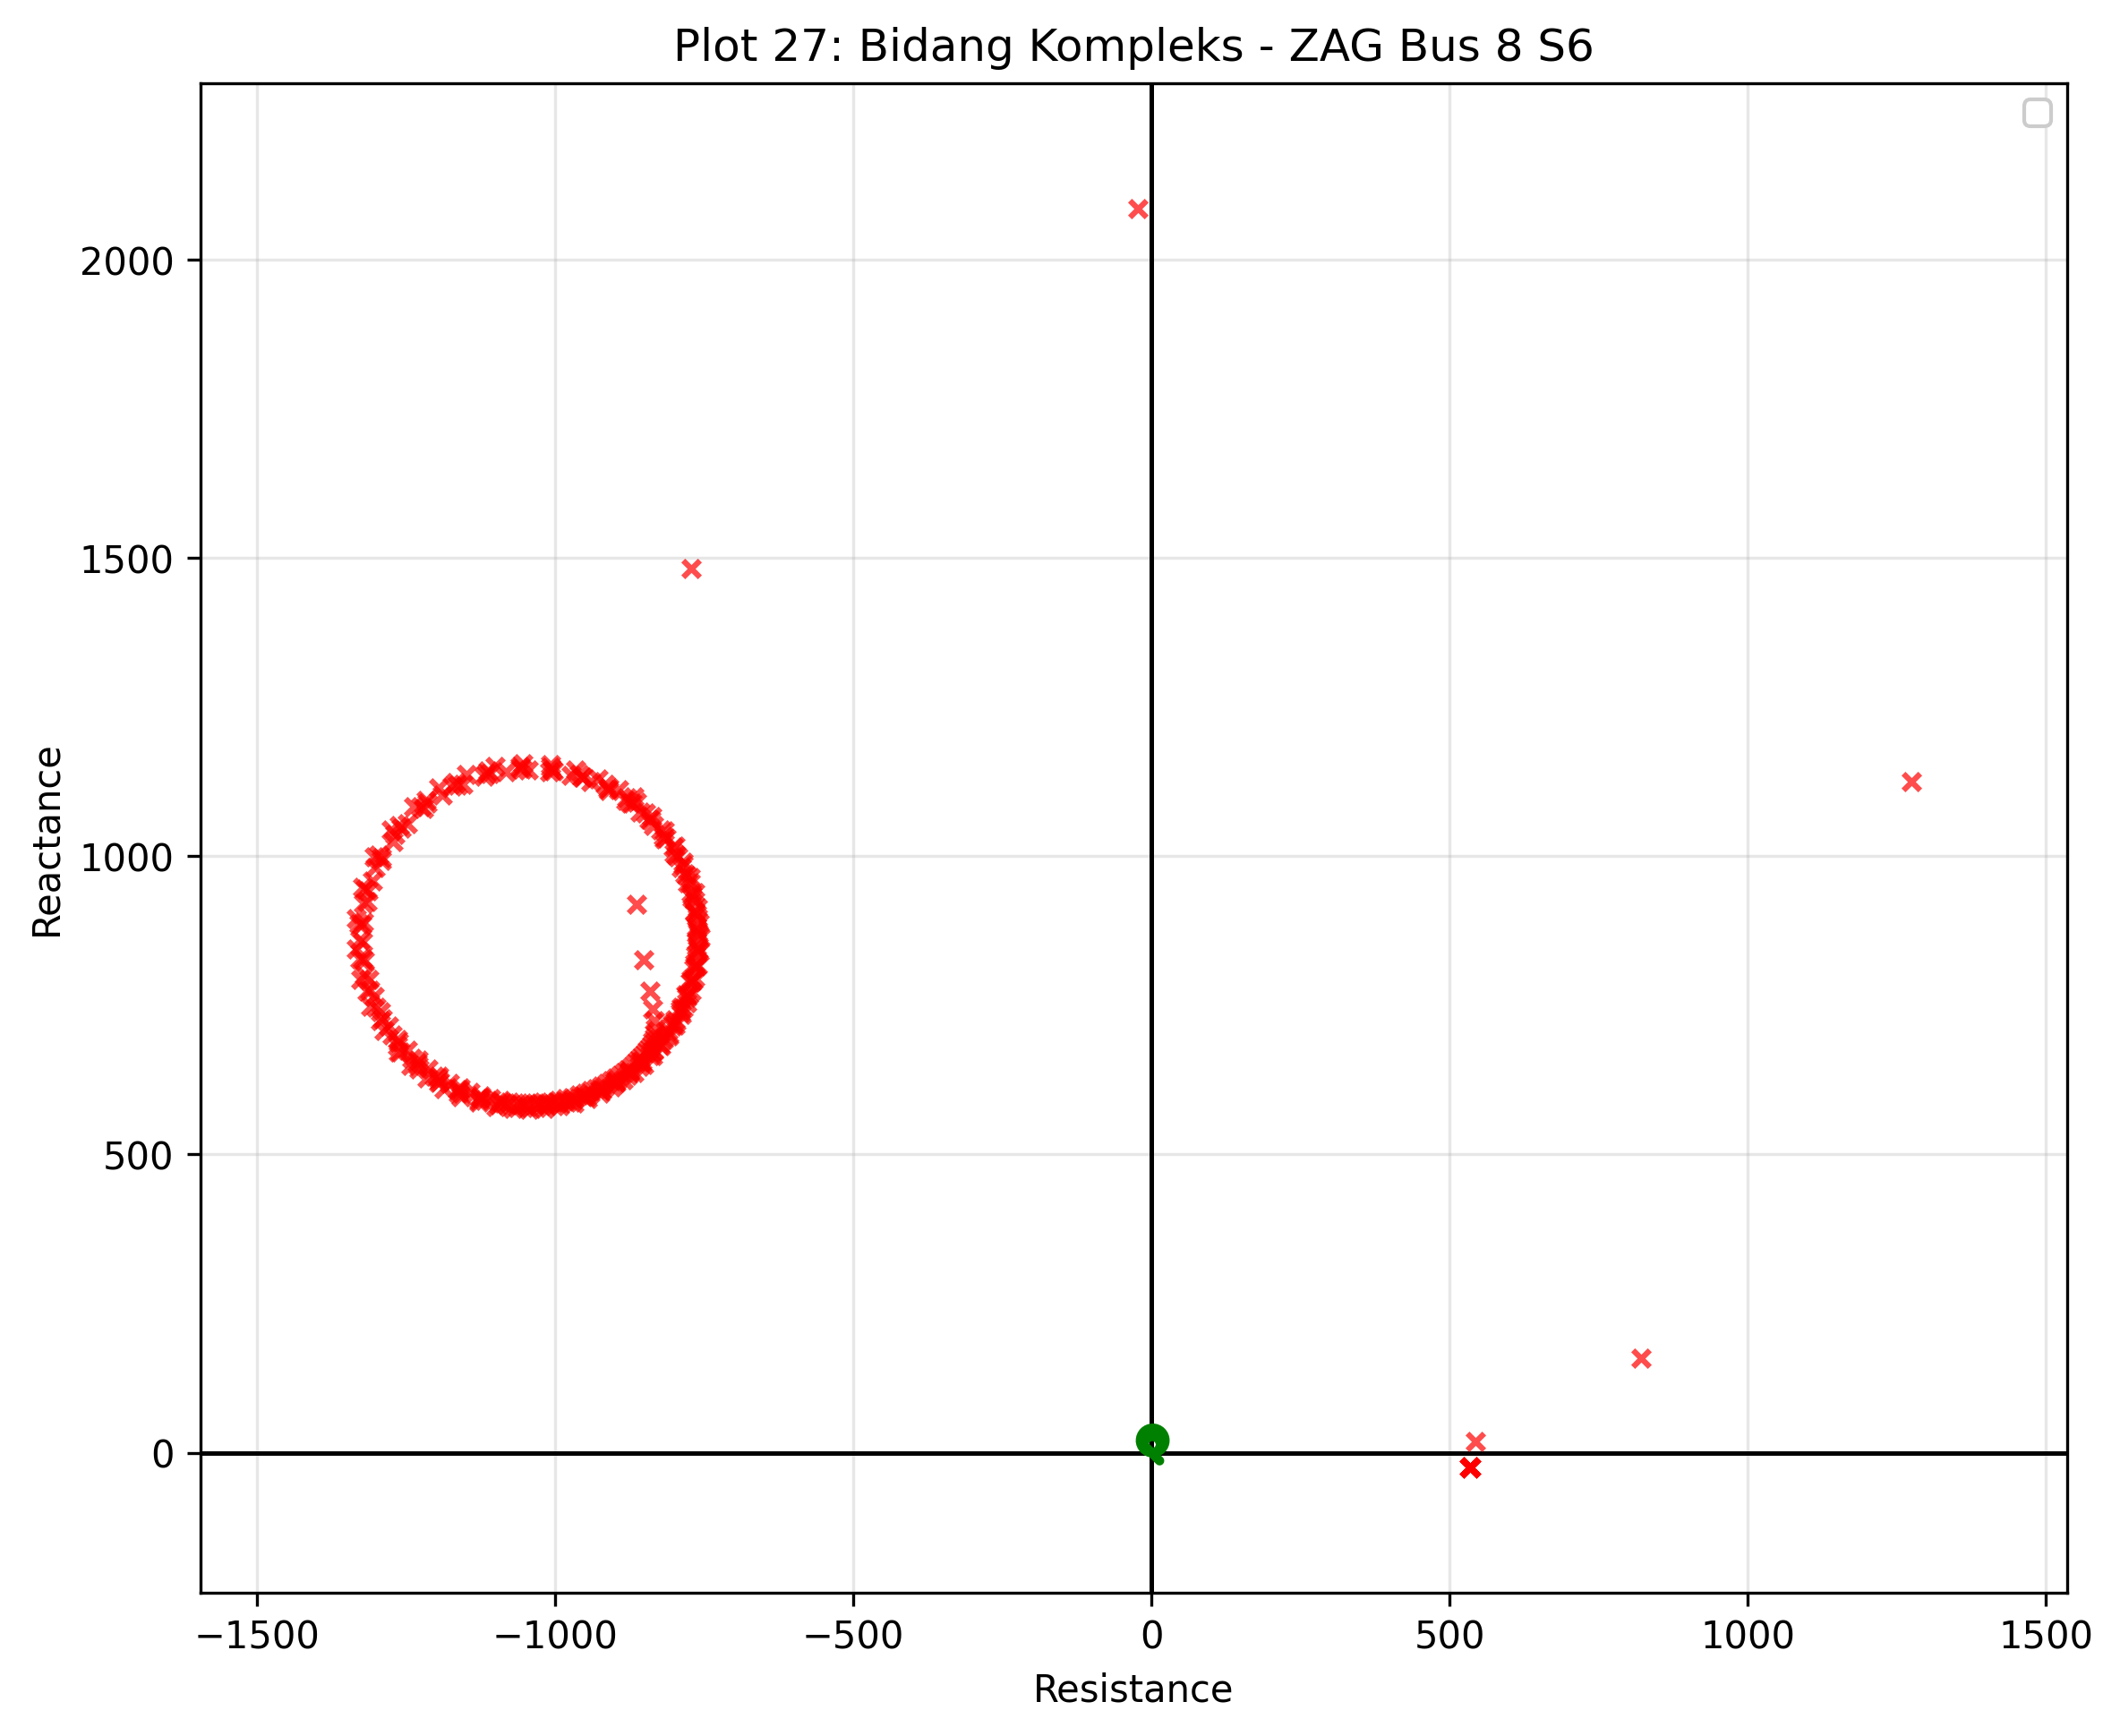
\includegraphics[width=\textwidth]{contents/chapter-4/PRIA_27_ZAG_Bus_8_S6.png}
        \caption{Seluruh Impedansi Tampak}
        \label{fig:PRIA_27_ZAG_Bus_8_S6}
    \end{subfigure}
    \hfill
    % Gambar sebelah kanan
    \begin{subfigure}[t]{0.48\textwidth}
        \centering
        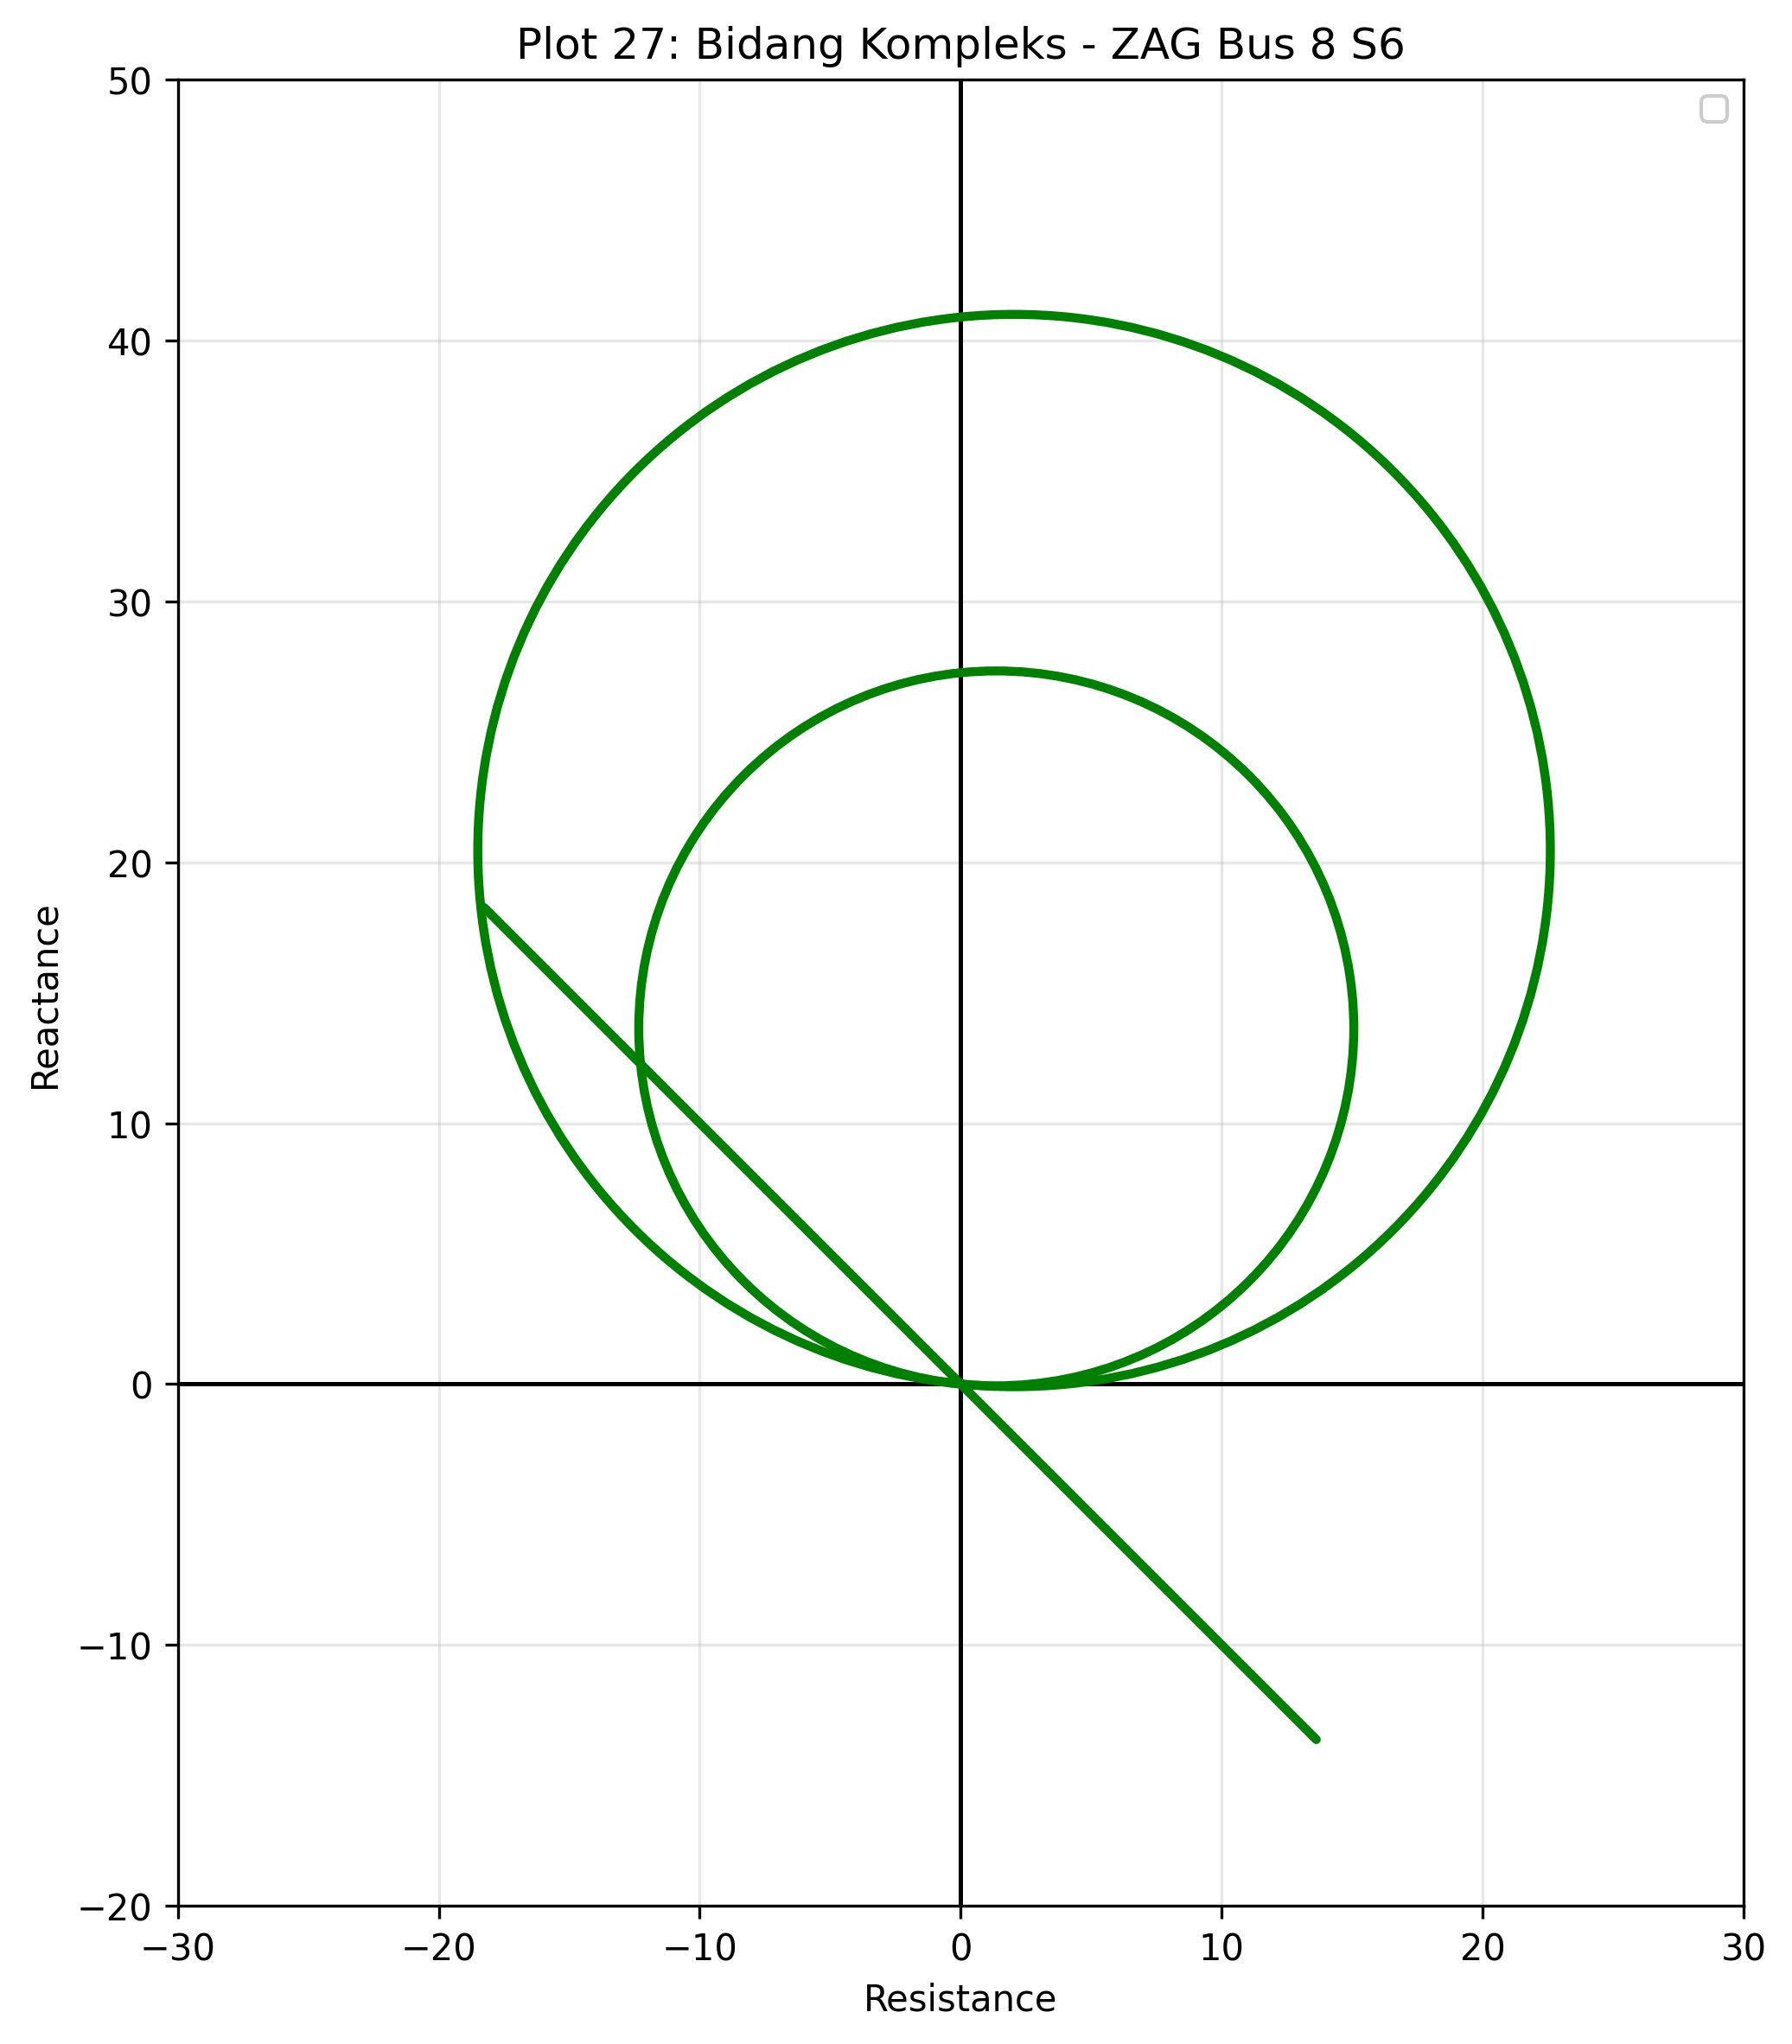
\includegraphics[width=\textwidth]{contents/chapter-4/PRIZI_27_ZAG_Bus_8_S6.png}
        \caption{Zoom In Pada Zona Proteksi}
        \label{fig:PRIZI_27_ZAG_Bus_8_S6}
    \end{subfigure}

    \caption{Impedansi Tampak ZAG Bus 8 Skenario 6}
    \label{fig:Impedansi_Tampak_ZAG_Bus_8_S6}
\end{figure}

Gambar \ref{fig:Impedansi_Tampak_ZAG_Bus_8_S6} menunjukkan bahwa impedansi tampak loop fasa A dengan ground yang dibaca oleh relay 21 sisi Bus 8 tidak masuk ke dalam zona proteksi. Kondisi ini sejalan dengan pembacaan arus sekunder CT pada Gambar \ref{fig:Bus_8_Ex_DLG_S6}, karena arus gangguan yang terbaca masih cukup kecil dan belum memenuhi syarat \textit{starting} untuk membuat relay aktif. Dengan mengacu pada kondisi dasar gangguan eksternal DLG pada Subbab \ref{subsec:tanpa_IBR_ex_dlg}, respons relay 21 sisi Bus 8 pada elemen ini dikategorikan mengalami \textit{misoperation}.


%%%%%%%%%%%%%%%%%%%%%%%%%%%%%%%%%%%%%%%%%%%%%%%%%%%%%%%%%%%%%%

% \begin{figure}[H]
%     \centering
%     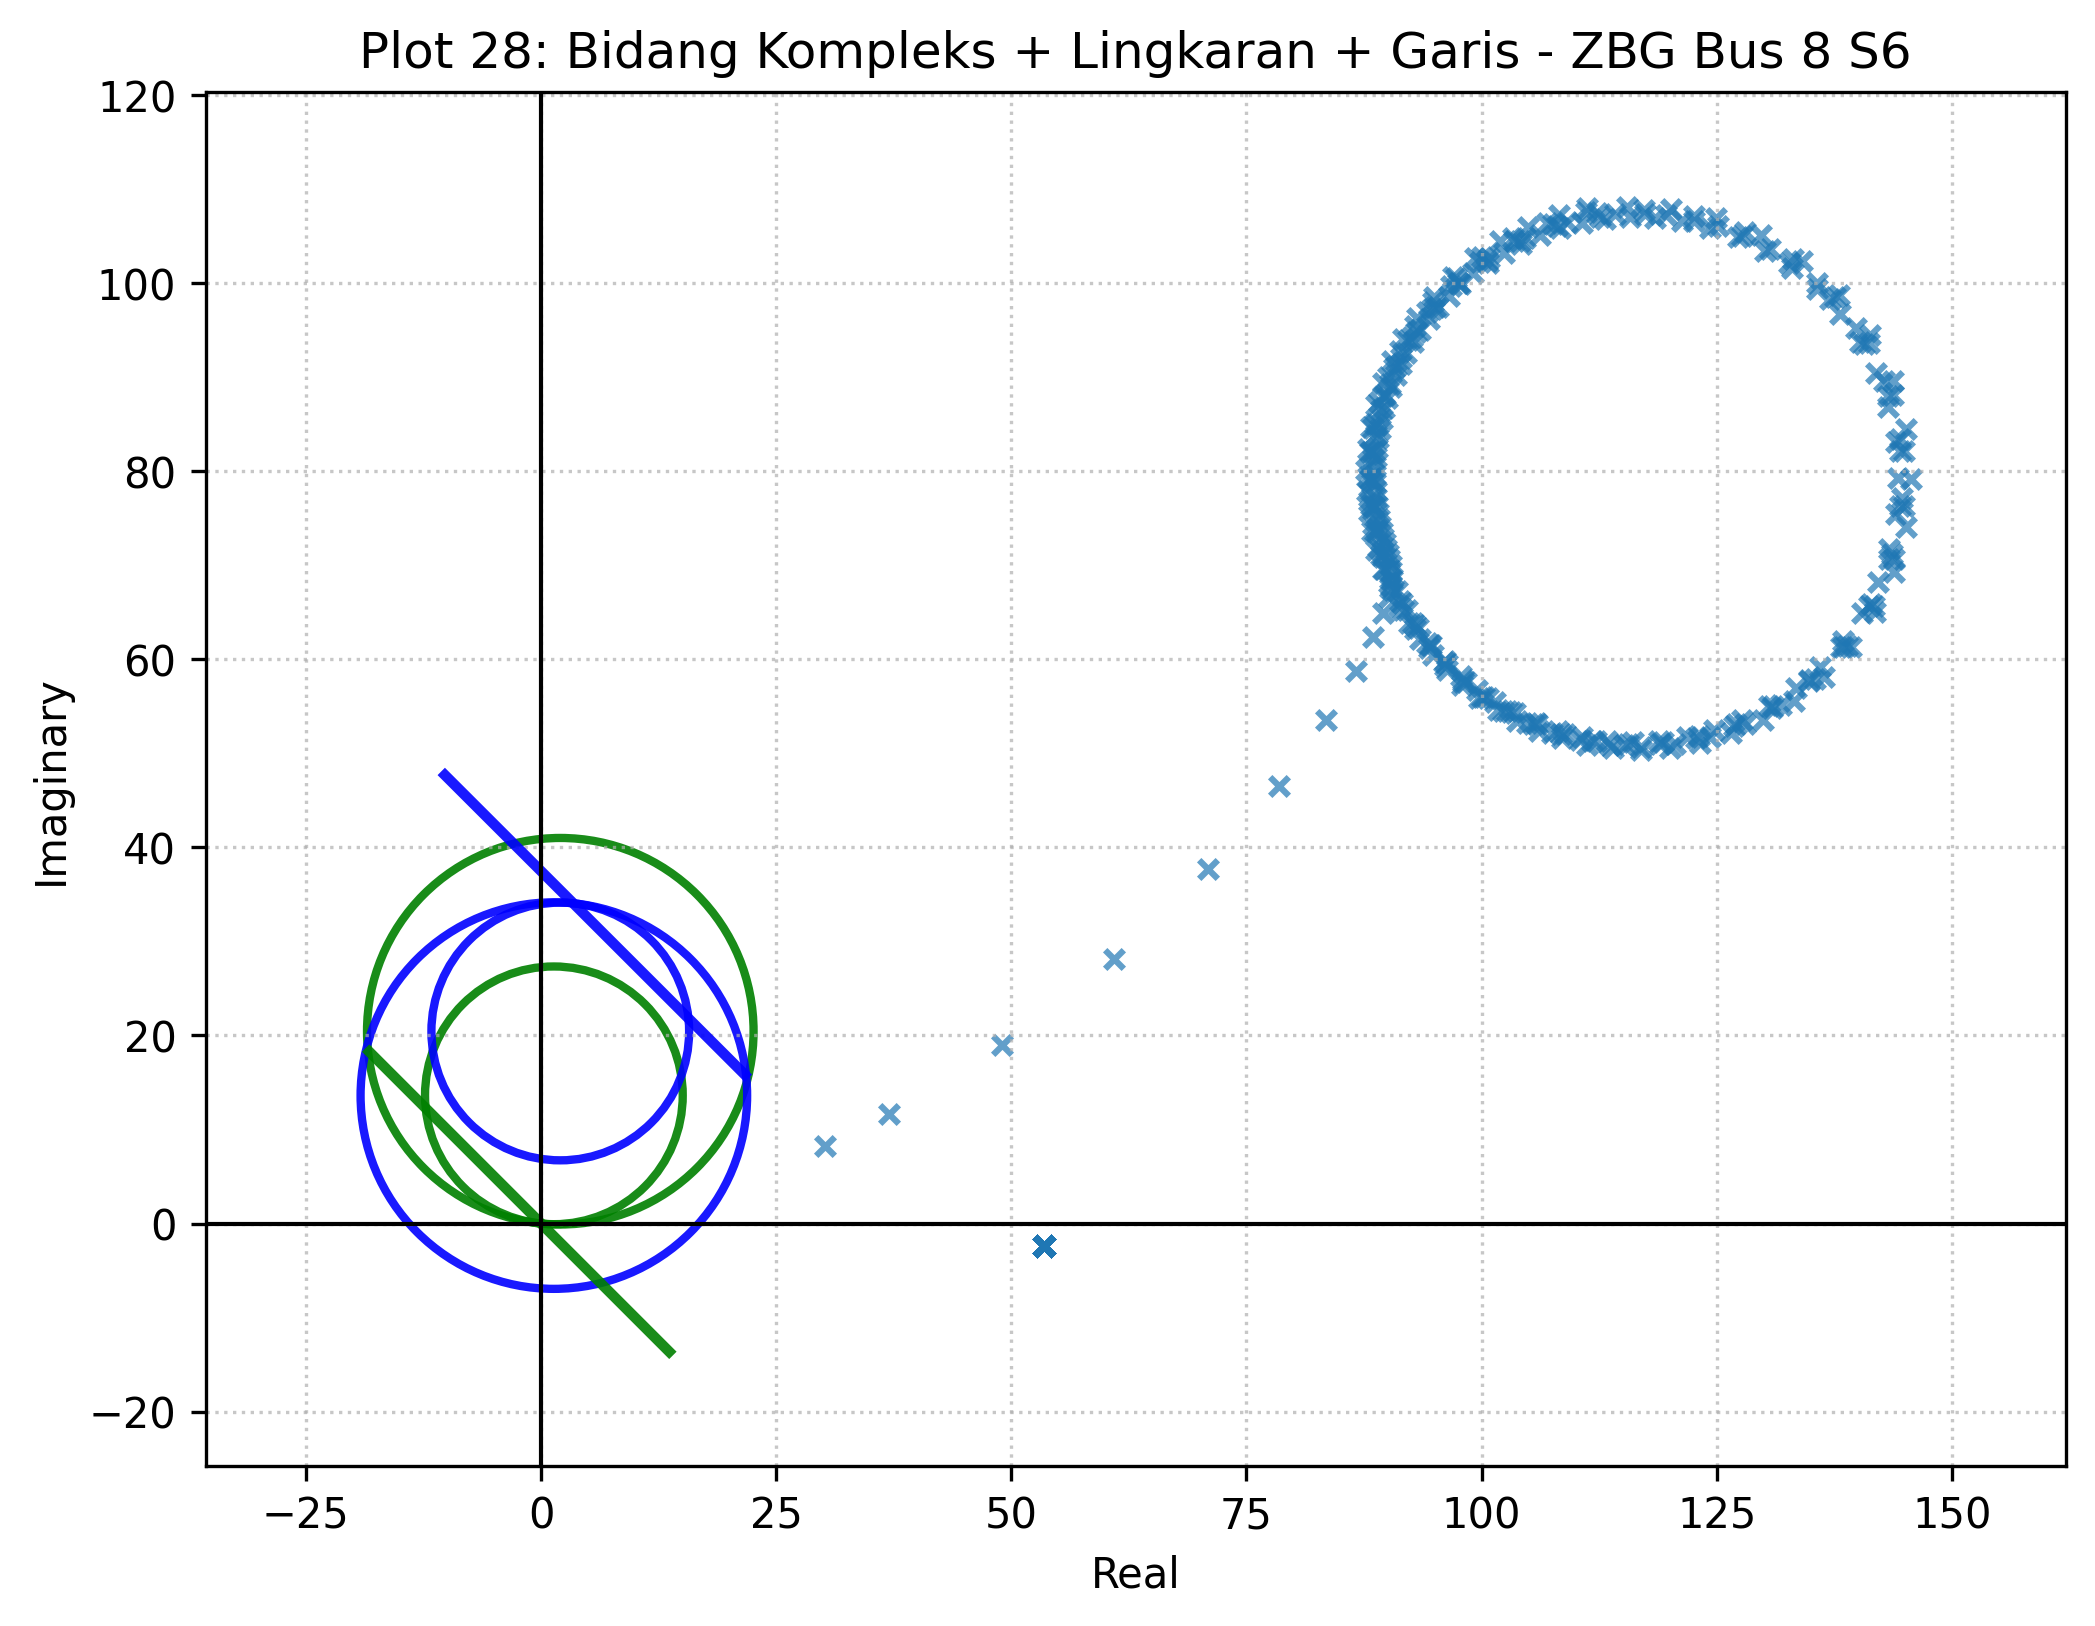
\includegraphics[width=0.8\textwidth]{contents/chapter-4/28_ZBG_Bus_8_S6_dengan_lingkaran_dan_garis.png}
%     \caption{Impedansi Tampak ZBG Bus 8 Skenario 6}
%     \label{fig:28_ZBG_Bus_8_S6_dengan_lingkaran_dan_garis}
% \end{figure}

%%%%%%%%%%%%%%%%%%%%%%%%%%%%%%%%%SISI PRIMER%%%%%%%%%%%%%%%%%%%%%%%%%%%%%%%%%%

% \begin{figure}[H]
%     \centering
%     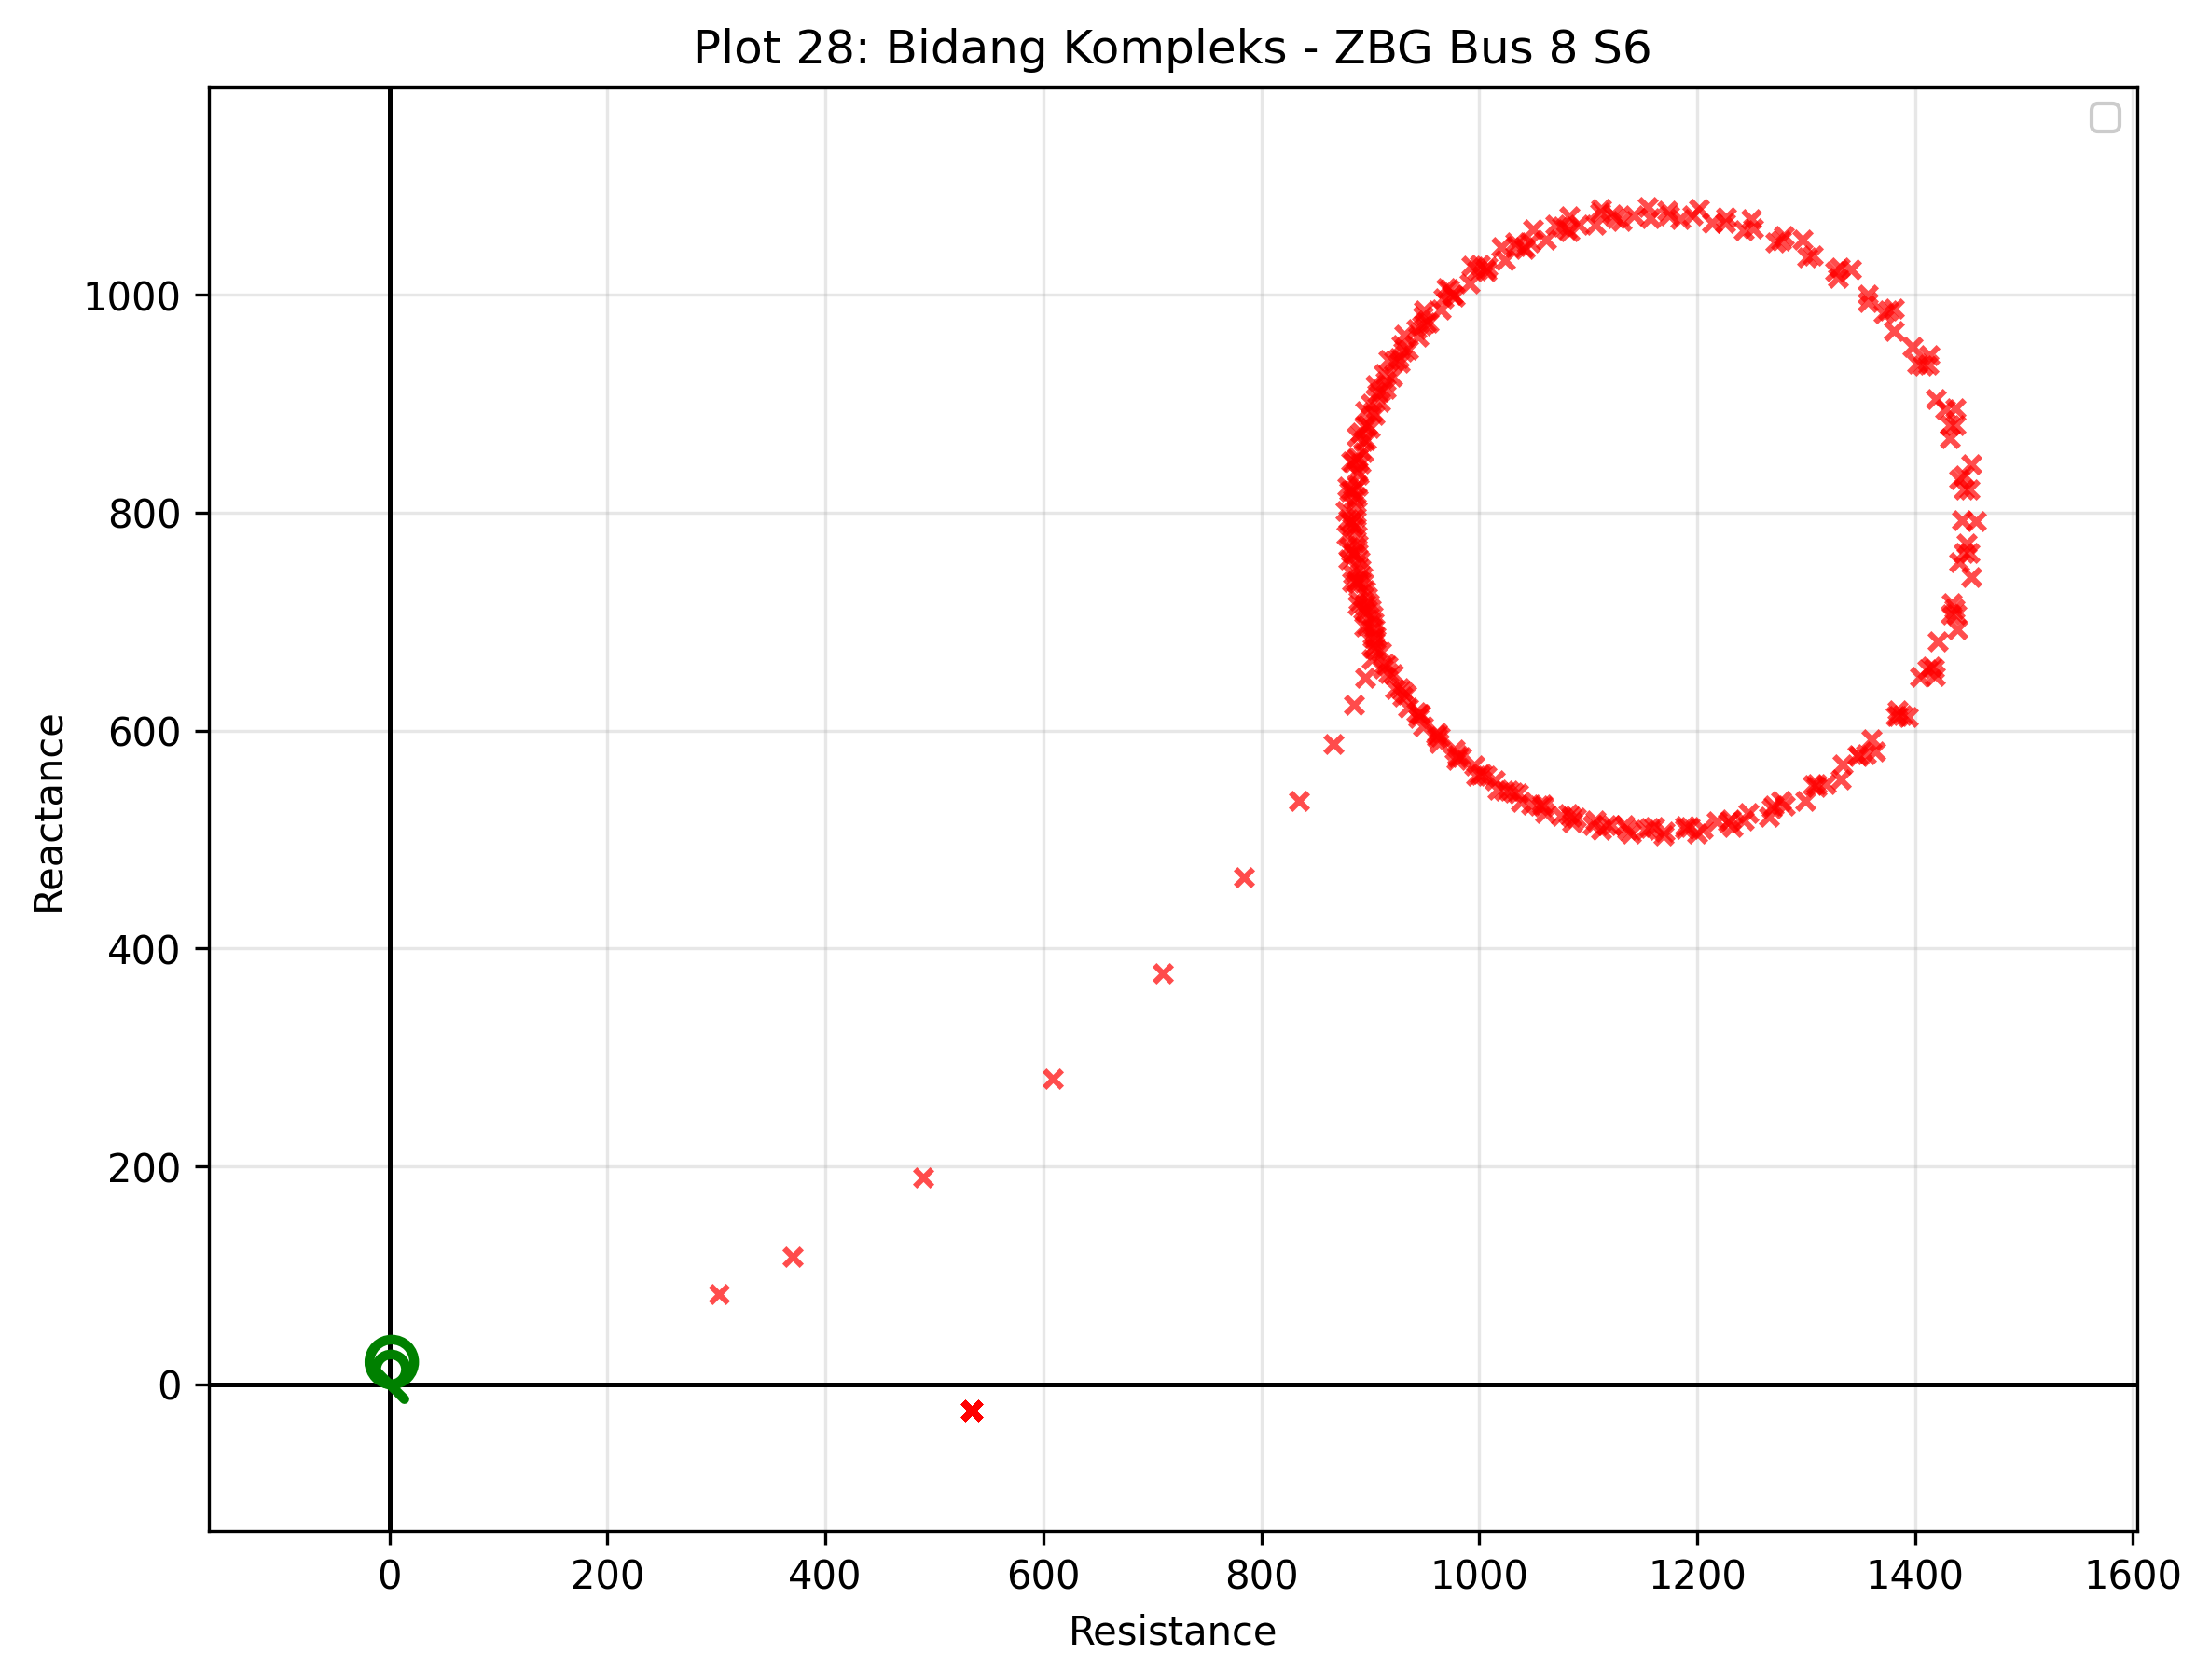
\includegraphics[width=0.8\textwidth]{contents/chapter-4/PRIA_28_ZBG_Bus_8_S6.png}
%     \caption{Impedansi Tampak ZBG Bus 8 Skenario 6}
%     \label{fig:PRIA_28_ZBG_Bus_8_S6}
% \end{figure}

% \begin{figure}[H]
%     \centering
%     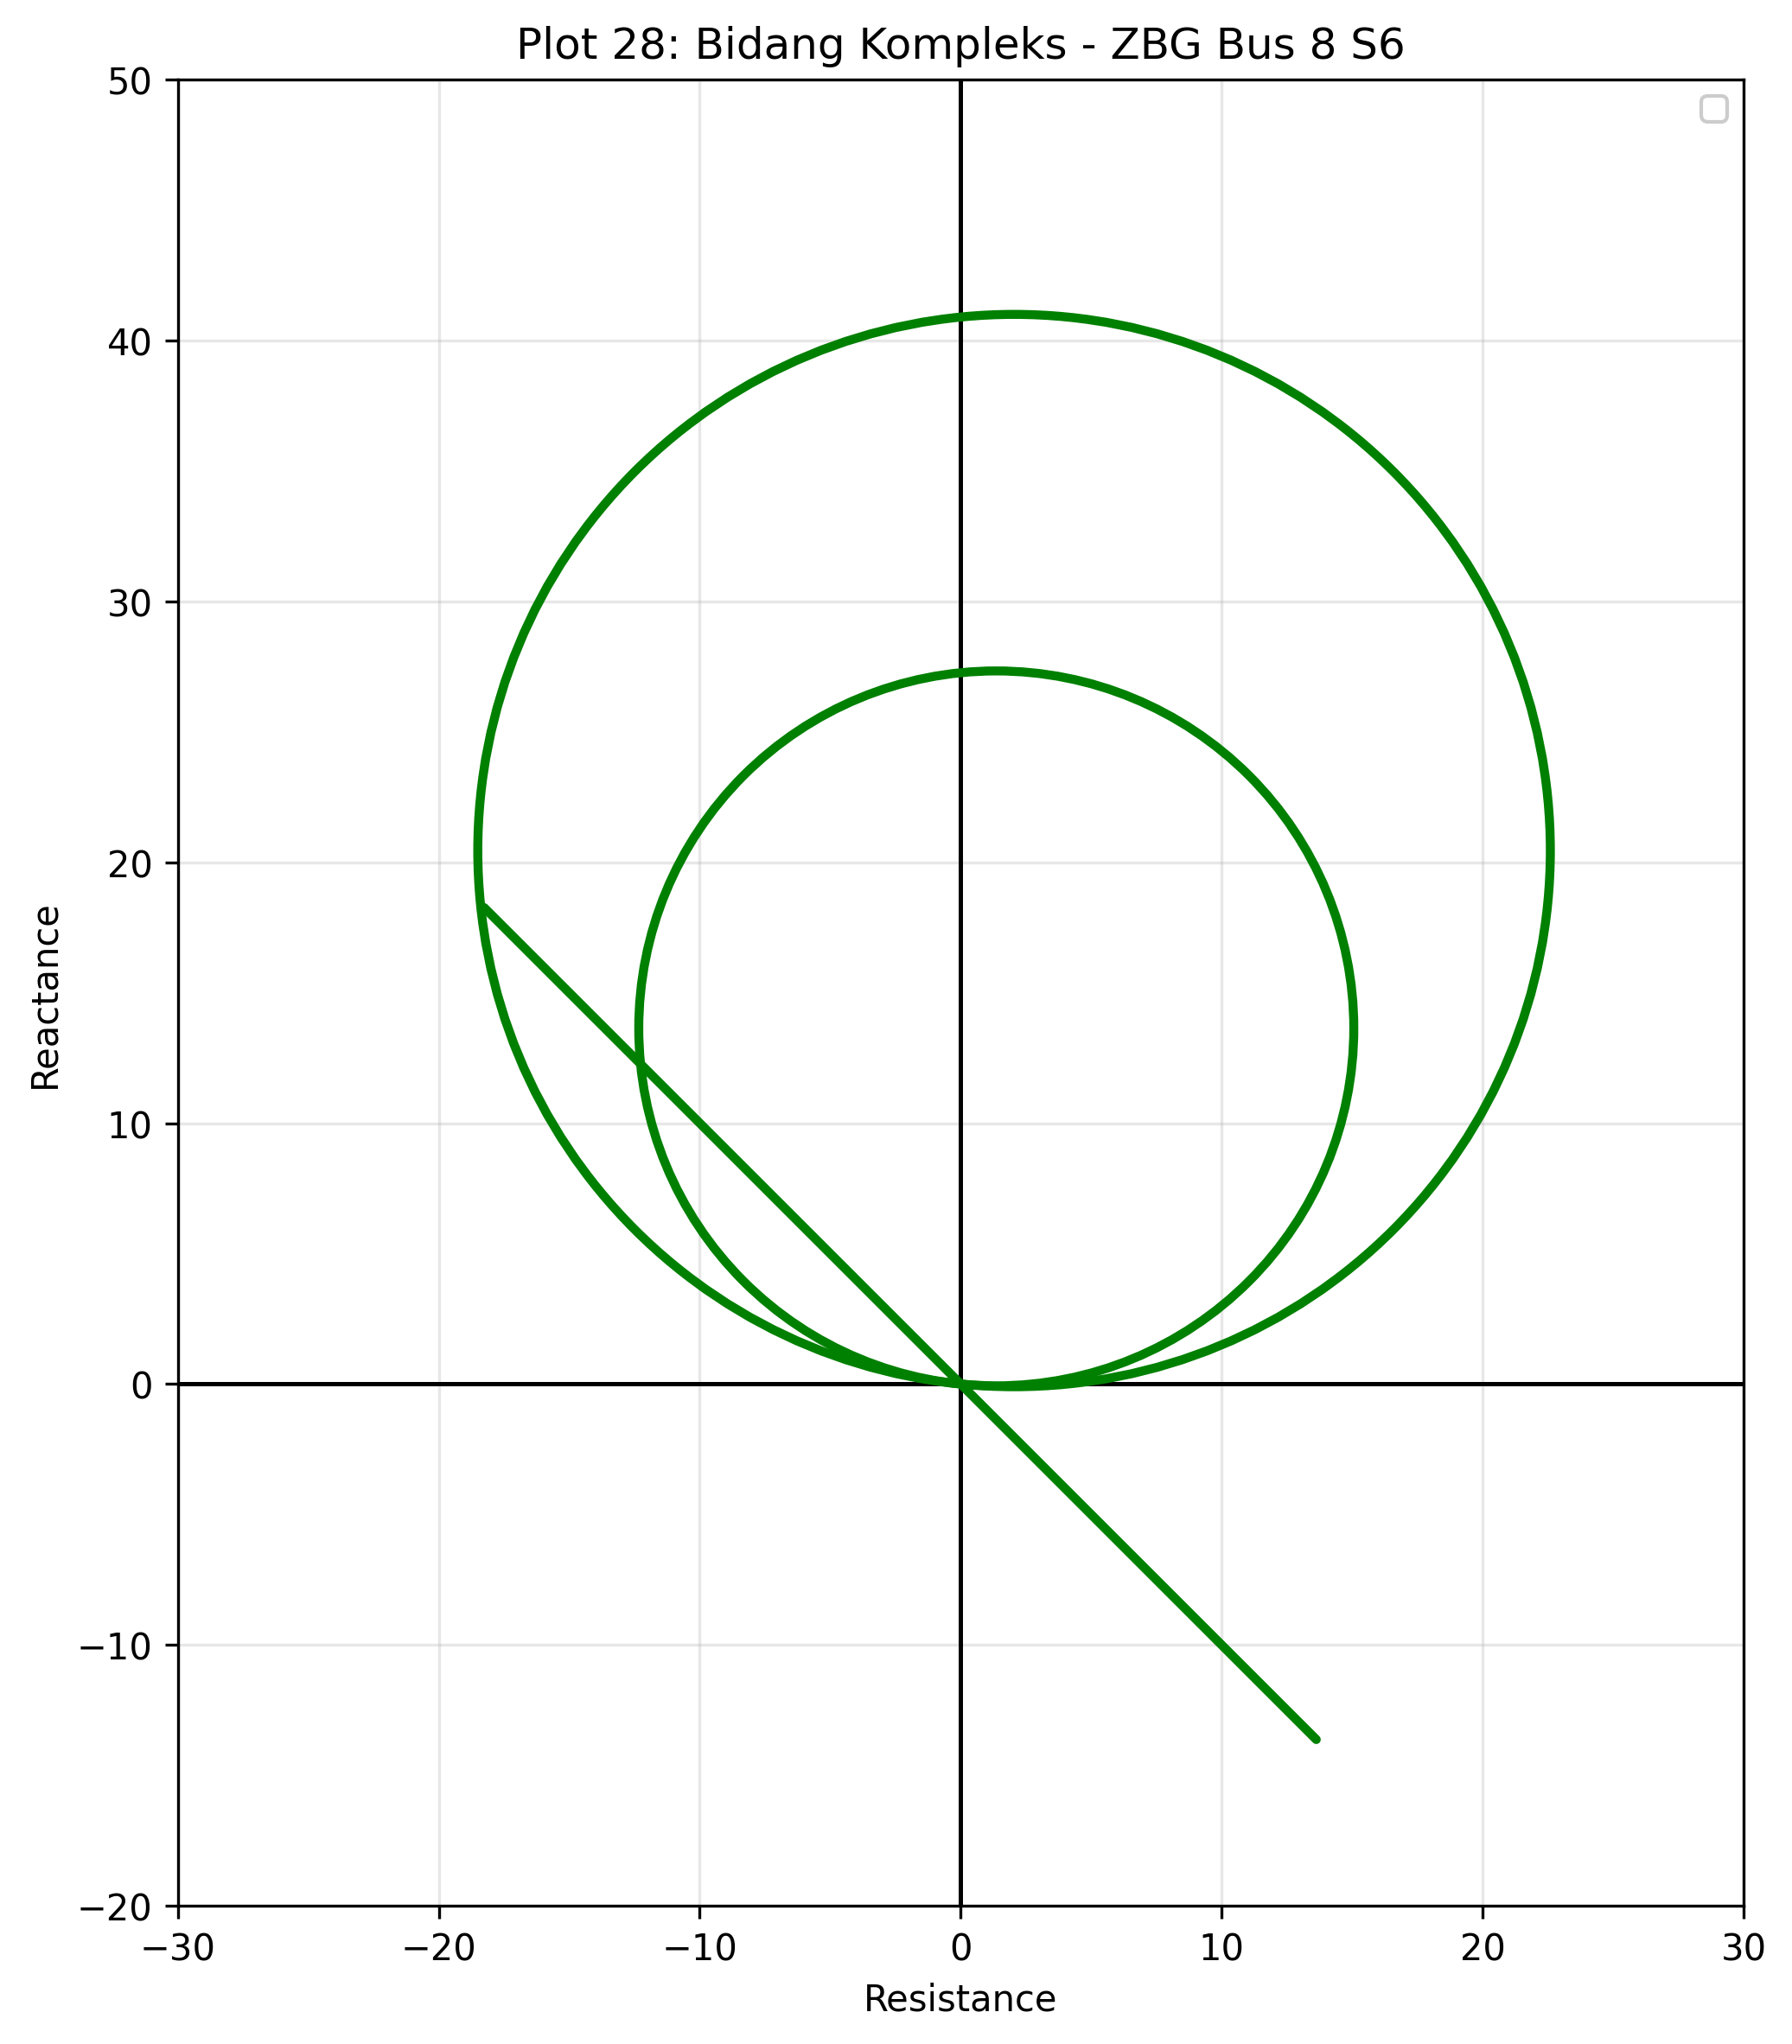
\includegraphics[width=0.8\textwidth]{contents/chapter-4/PRIZI_28_ZBG_Bus_8_S6.png}
%     \caption{Impedansi Tampak ZBG Bus 8 Skenario 6}
%     \label{fig:PRIZI_28_ZBG_Bus_8_S6}
% \end{figure}

\begin{figure}[H]
    \centering

    % Gambar sebelah kiri
    \begin{subfigure}[t]{0.48\textwidth}
        \centering
        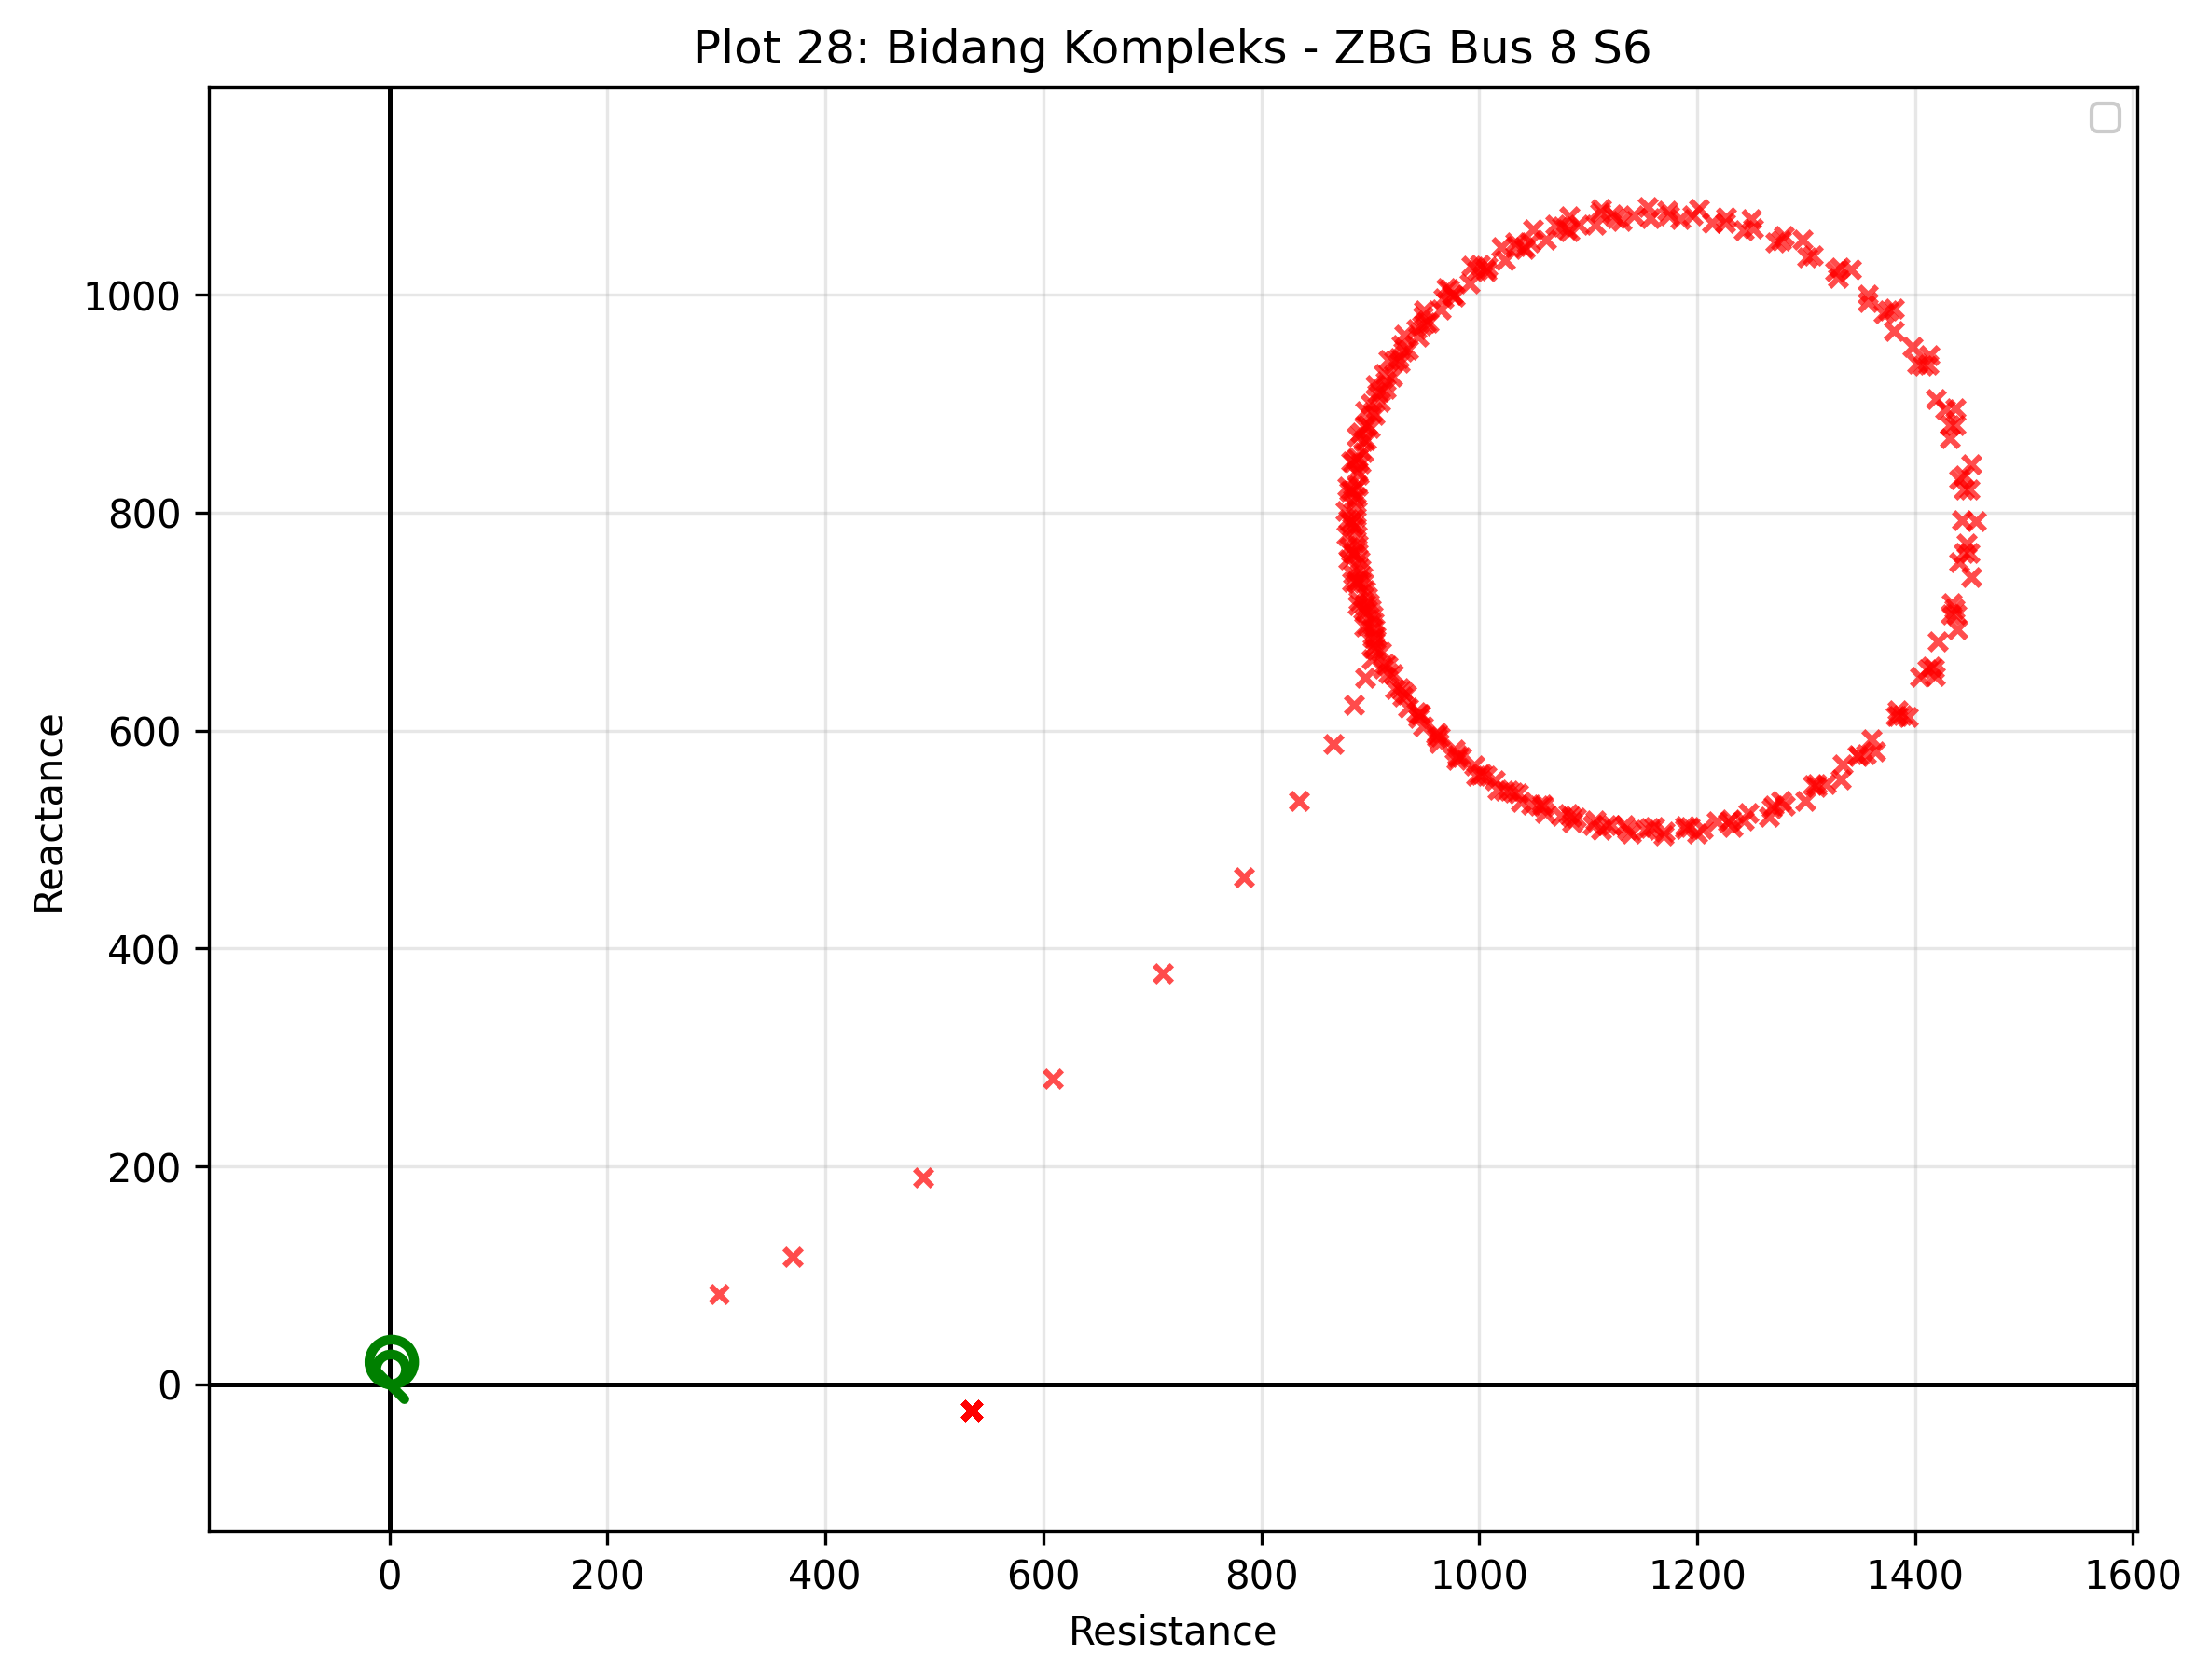
\includegraphics[width=\textwidth]{contents/chapter-4/PRIA_28_ZBG_Bus_8_S6.png}
        \caption{Seluruh Impedansi Tampak}
        \label{fig:PRIA_28_ZBG_Bus_8_S6}
    \end{subfigure}
    \hfill
    % Gambar sebelah kanan
    \begin{subfigure}[t]{0.48\textwidth}
        \centering
        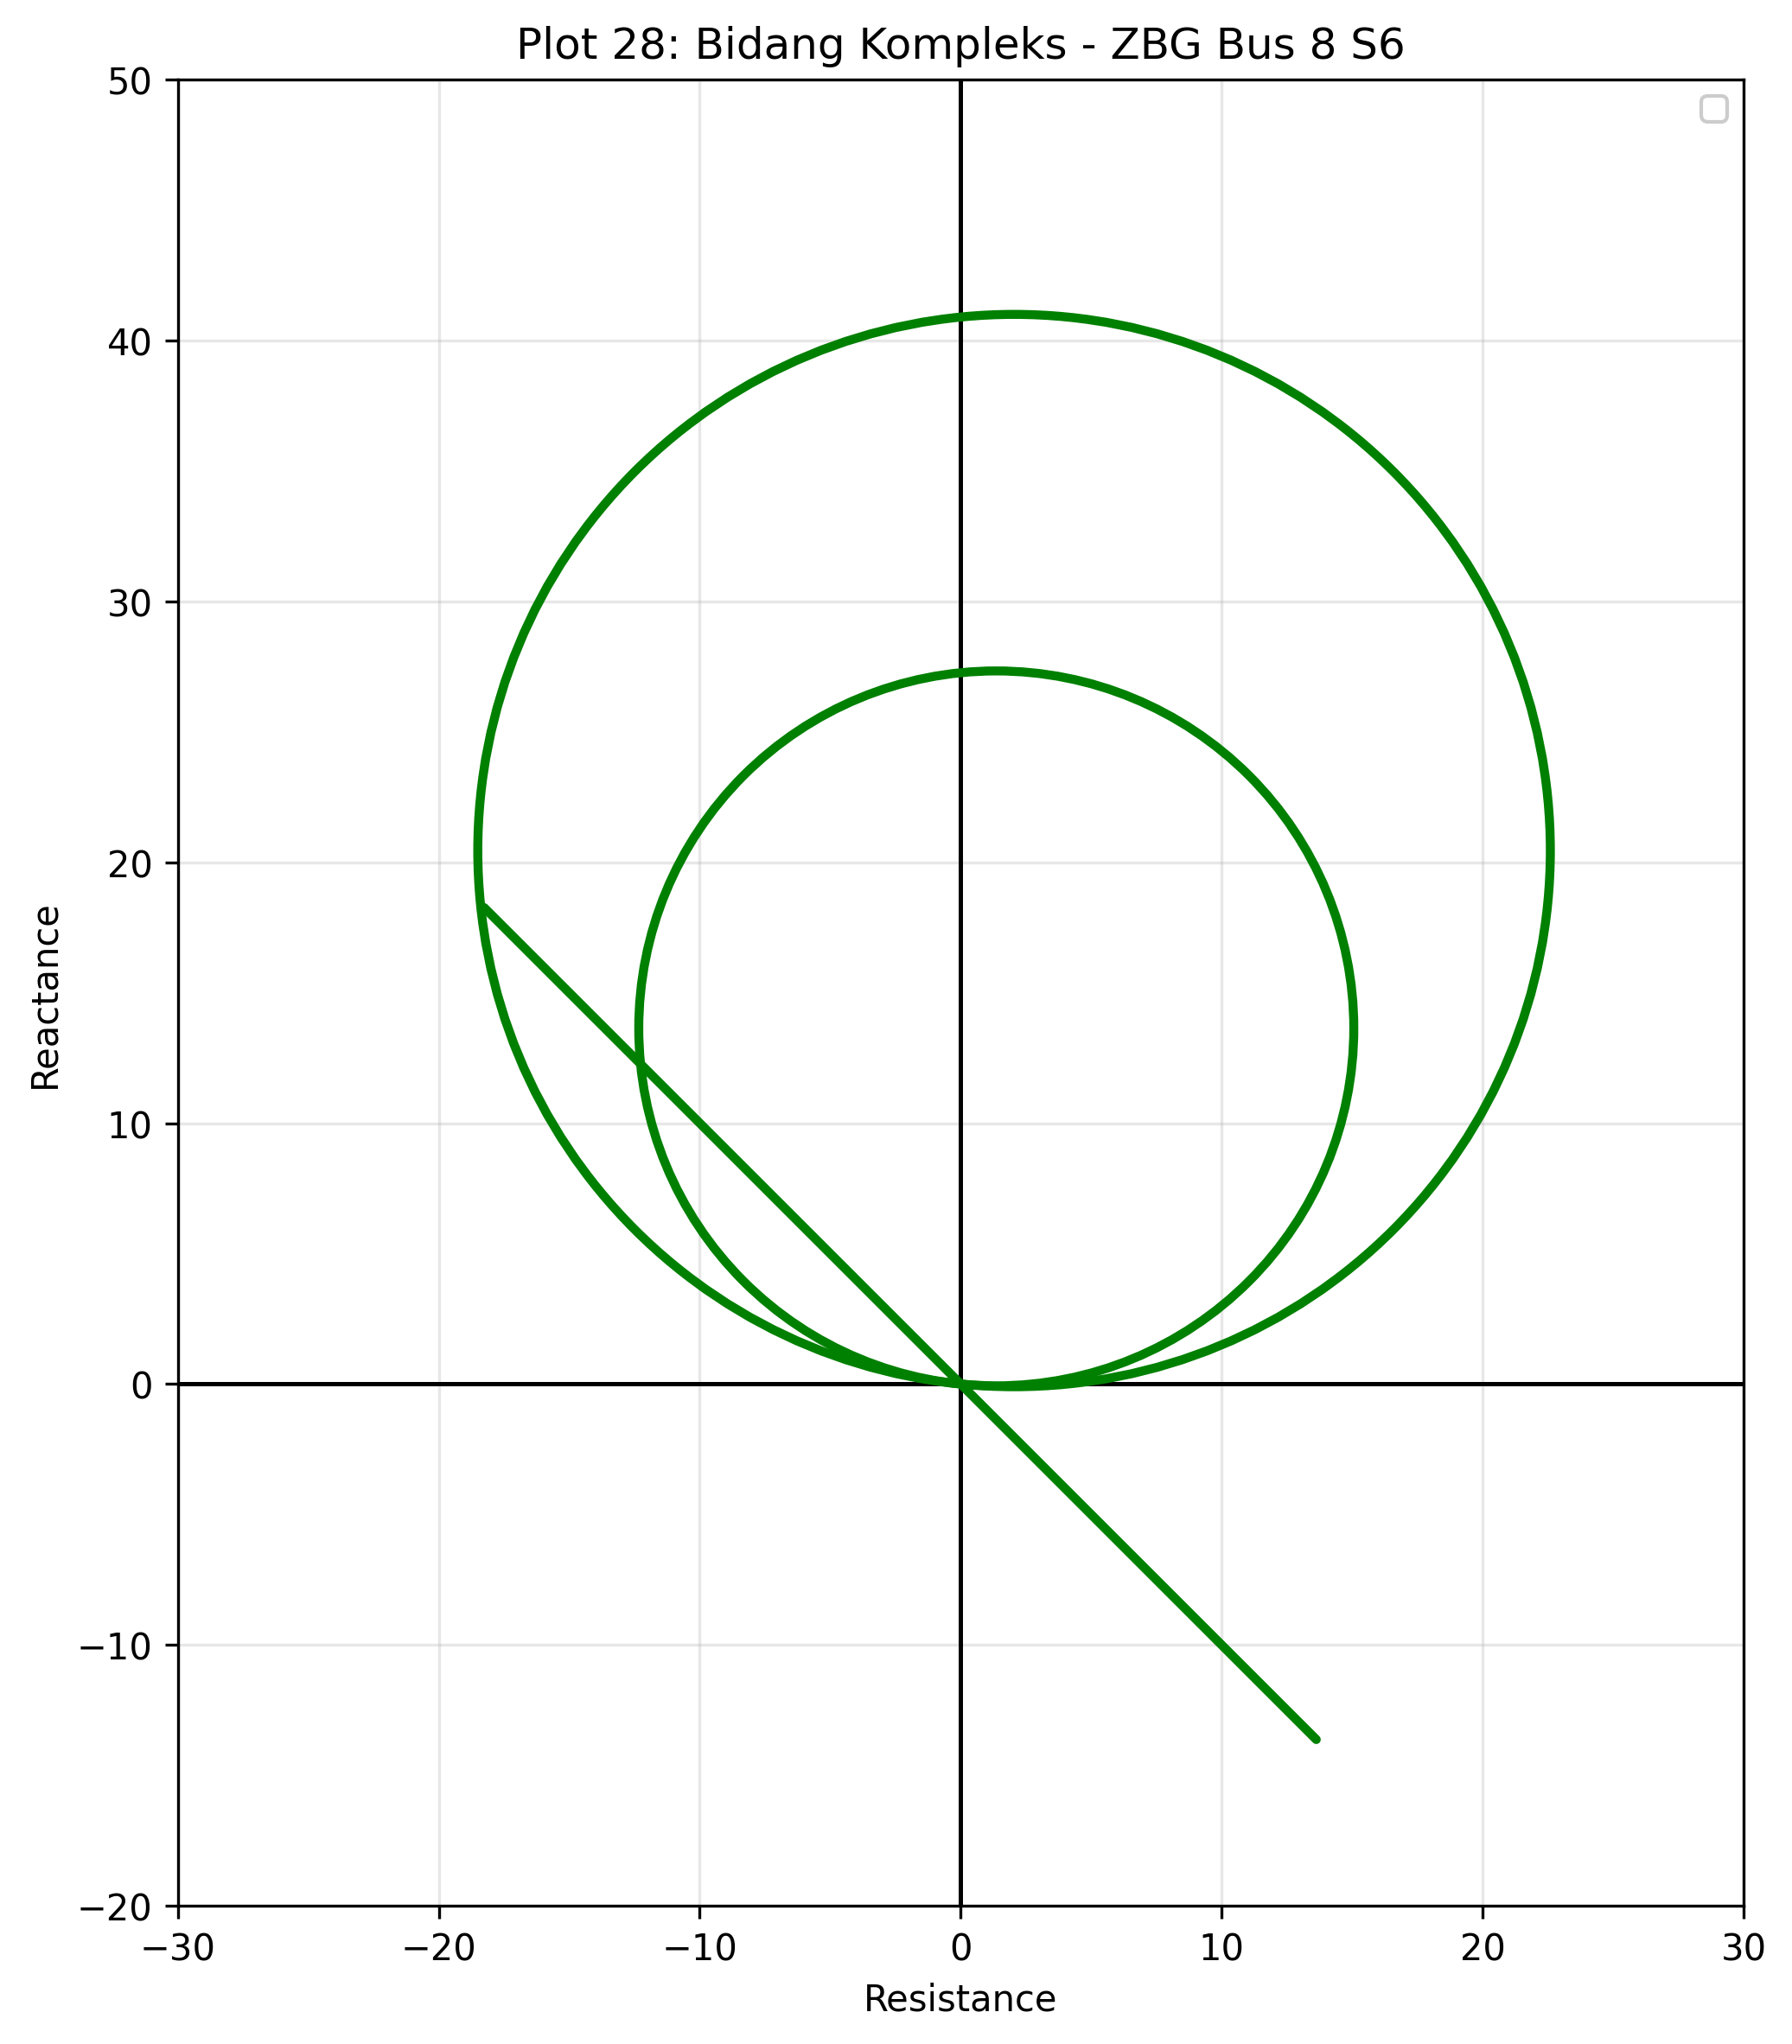
\includegraphics[width=\textwidth]{contents/chapter-4/PRIZI_28_ZBG_Bus_8_S6.png}
        \caption{Zoom In Pada Zona Proteksi}
        \label{fig:PRIZI_28_ZBG_Bus_8_S6}
    \end{subfigure}

    \caption{Impedansi Tampak ZBG Bus 8 Skenario 6}
    \label{fig:Impedansi_Tampak_ZBG_Bus_8_S6}
\end{figure}

Gambar \ref{fig:Impedansi_Tampak_ZBG_Bus_8_S6} menunjukkan bahwa impedansi tampak loop fasa B dengan ground yang dibaca oleh relay 21 sisi Bus 8 juga tidak masuk ke dalam zona proteksi. Hasil tersebut masih konsisten dengan arus sekunder CT pada Gambar \ref{fig:Bus_8_Ex_DLG_S6}, yaitu arus gangguan belum memenuhi syarat \textit{starting} untuk membuat relay aktif. Oleh karena itu, jika dibandingkan dengan acuan gangguan eksternal DLG pada Subbab \ref{subsec:tanpa_IBR_ex_dlg}, respons relay 21 sisi Bus 8 pada elemen ini juga menunjukkan \textit{misoperation}.


%%%%%%%%%%%%%%%%%%%%%%%%%%%%%%%%%%%%%%%%%%%%%%%%%%%%%%%%%%%%%%

% \begin{figure}[H]
%     \centering
%     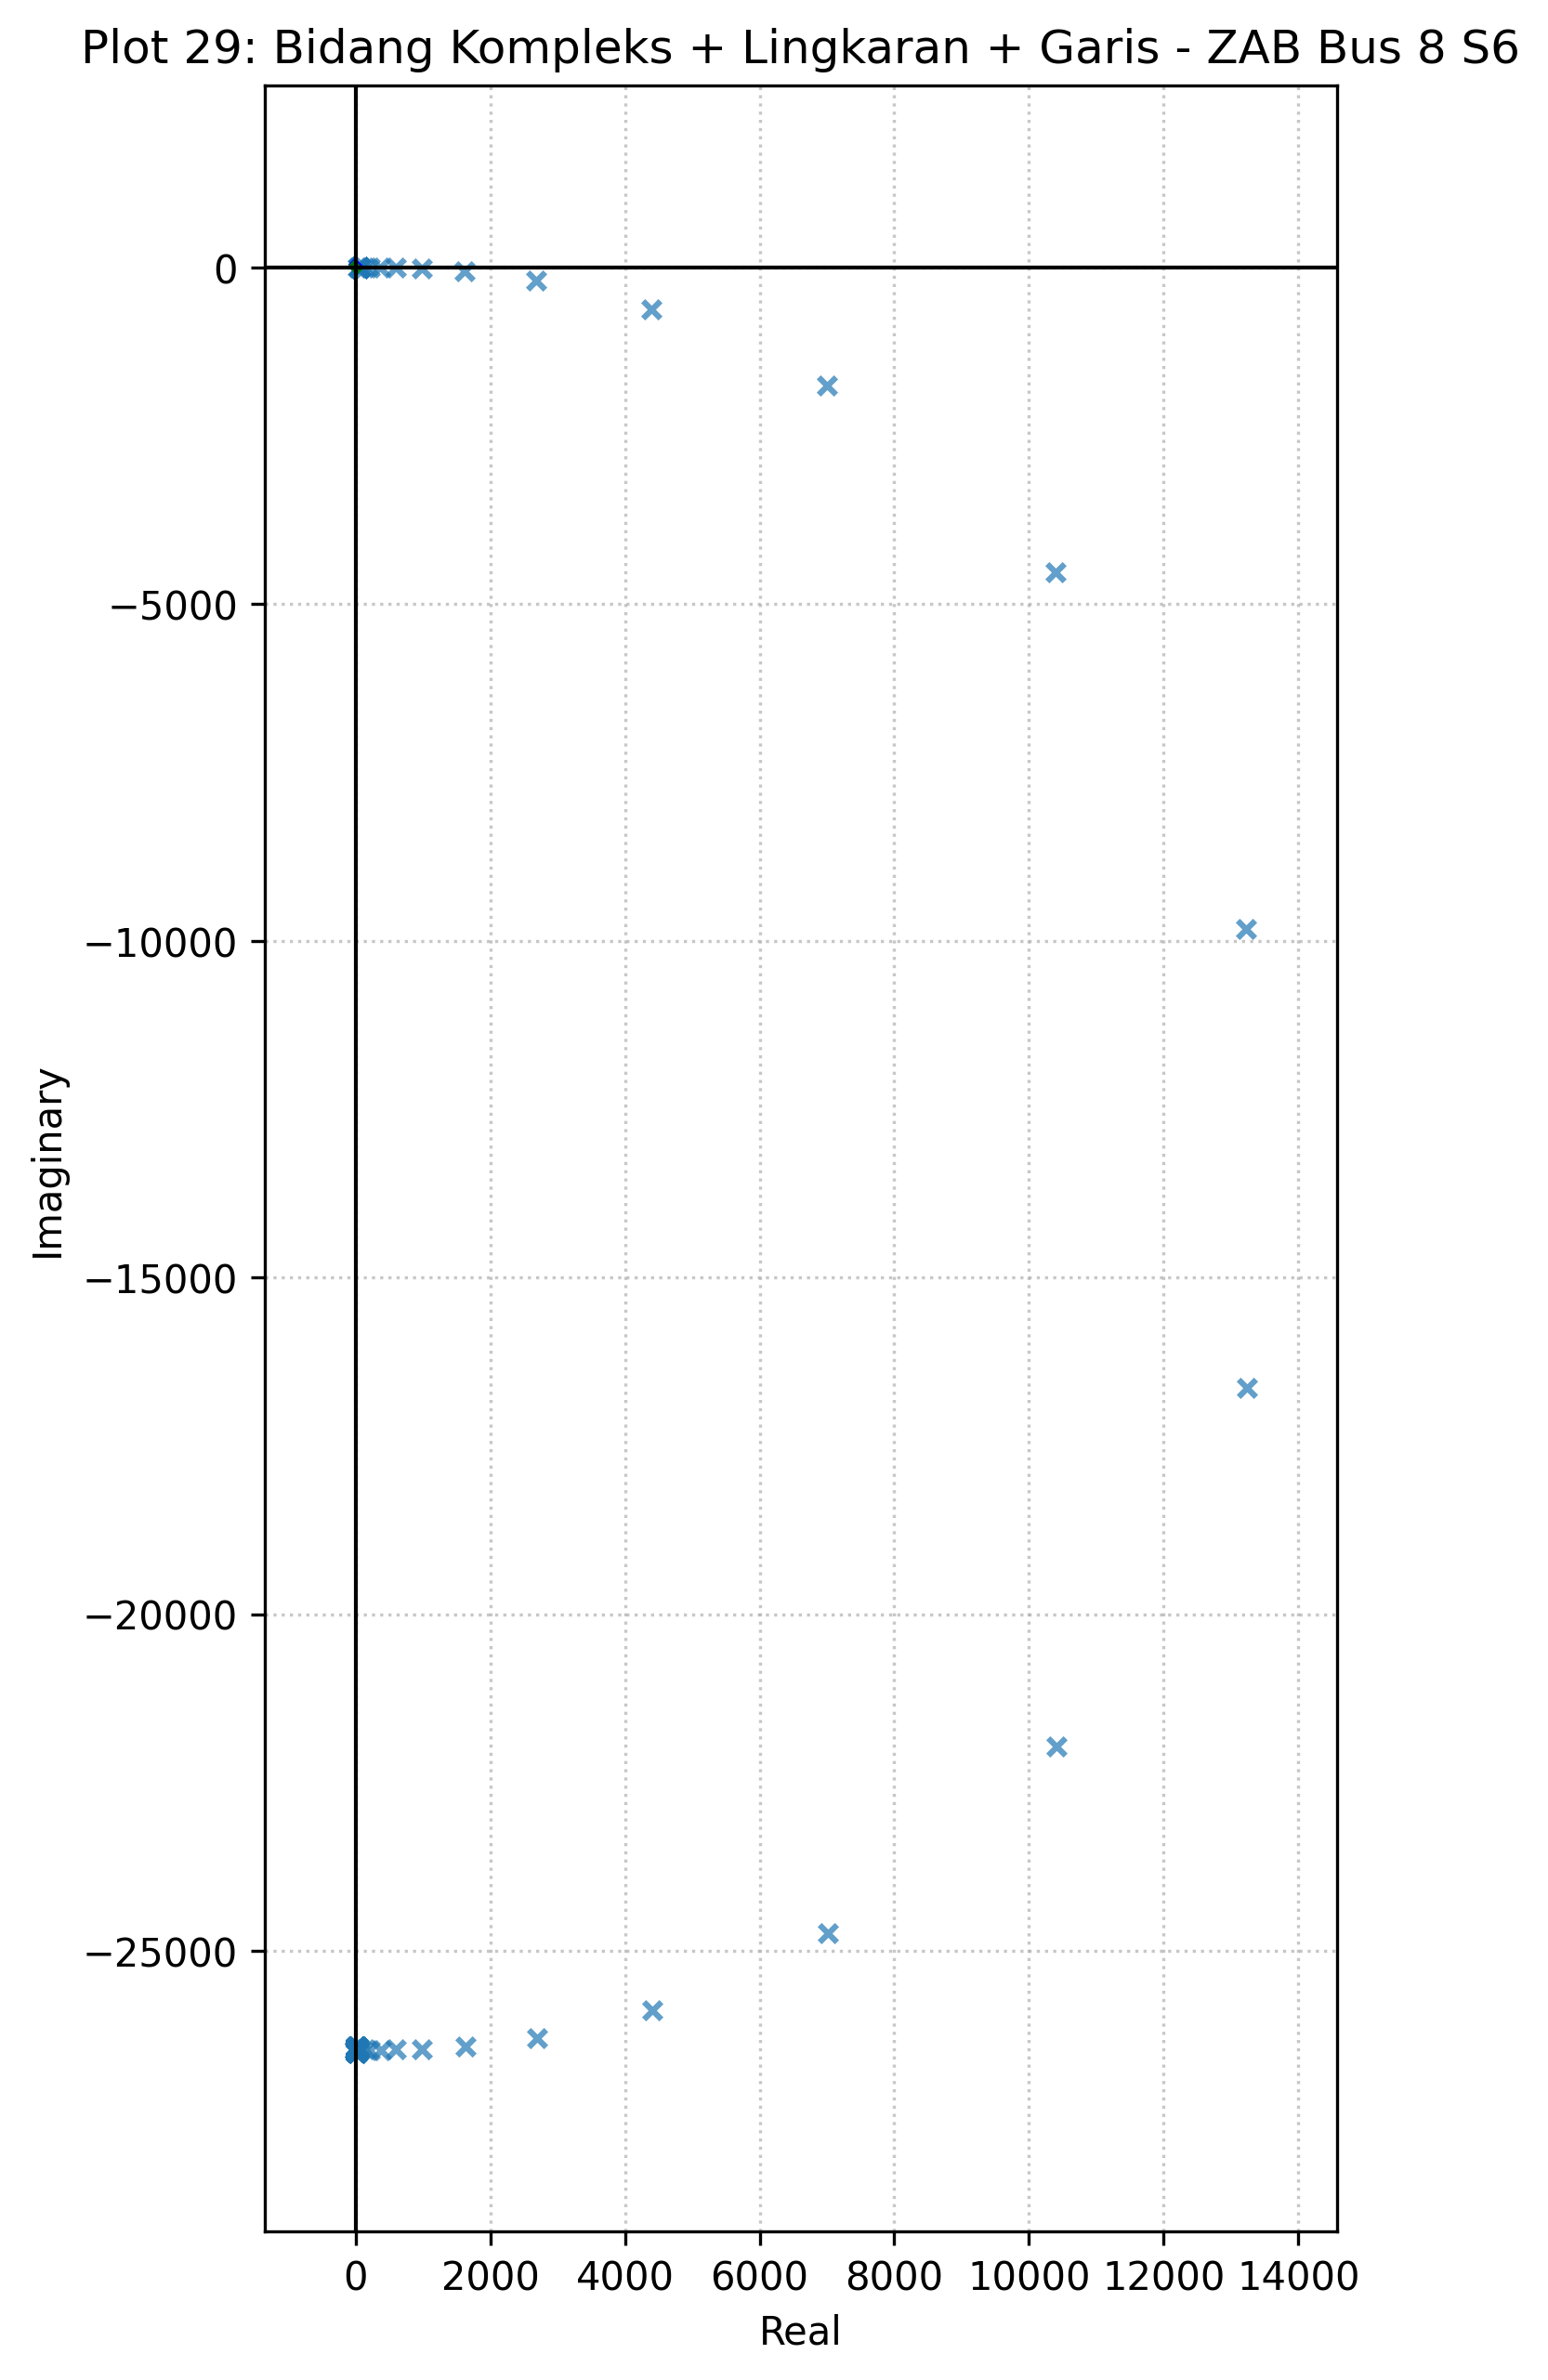
\includegraphics[width=0.8\textwidth]{contents/chapter-4/29_ZAB_Bus_8_S6_dengan_lingkaran_dan_garis.png}
%     \caption{Impedansi Tampak ZAB Bus 8 Skenario 6}
%     \label{fig:29_ZAB_Bus_8_S6_dengan_lingkaran_dan_garis}
% \end{figure}

%%%%%%%%%%%%%%%%%%%%%%%%%%%%%%%%%SISI PRIMER%%%%%%%%%%%%%%%%%%%%%%%%%%%%%%%%%%

% \begin{figure}[H]
%     \centering
%     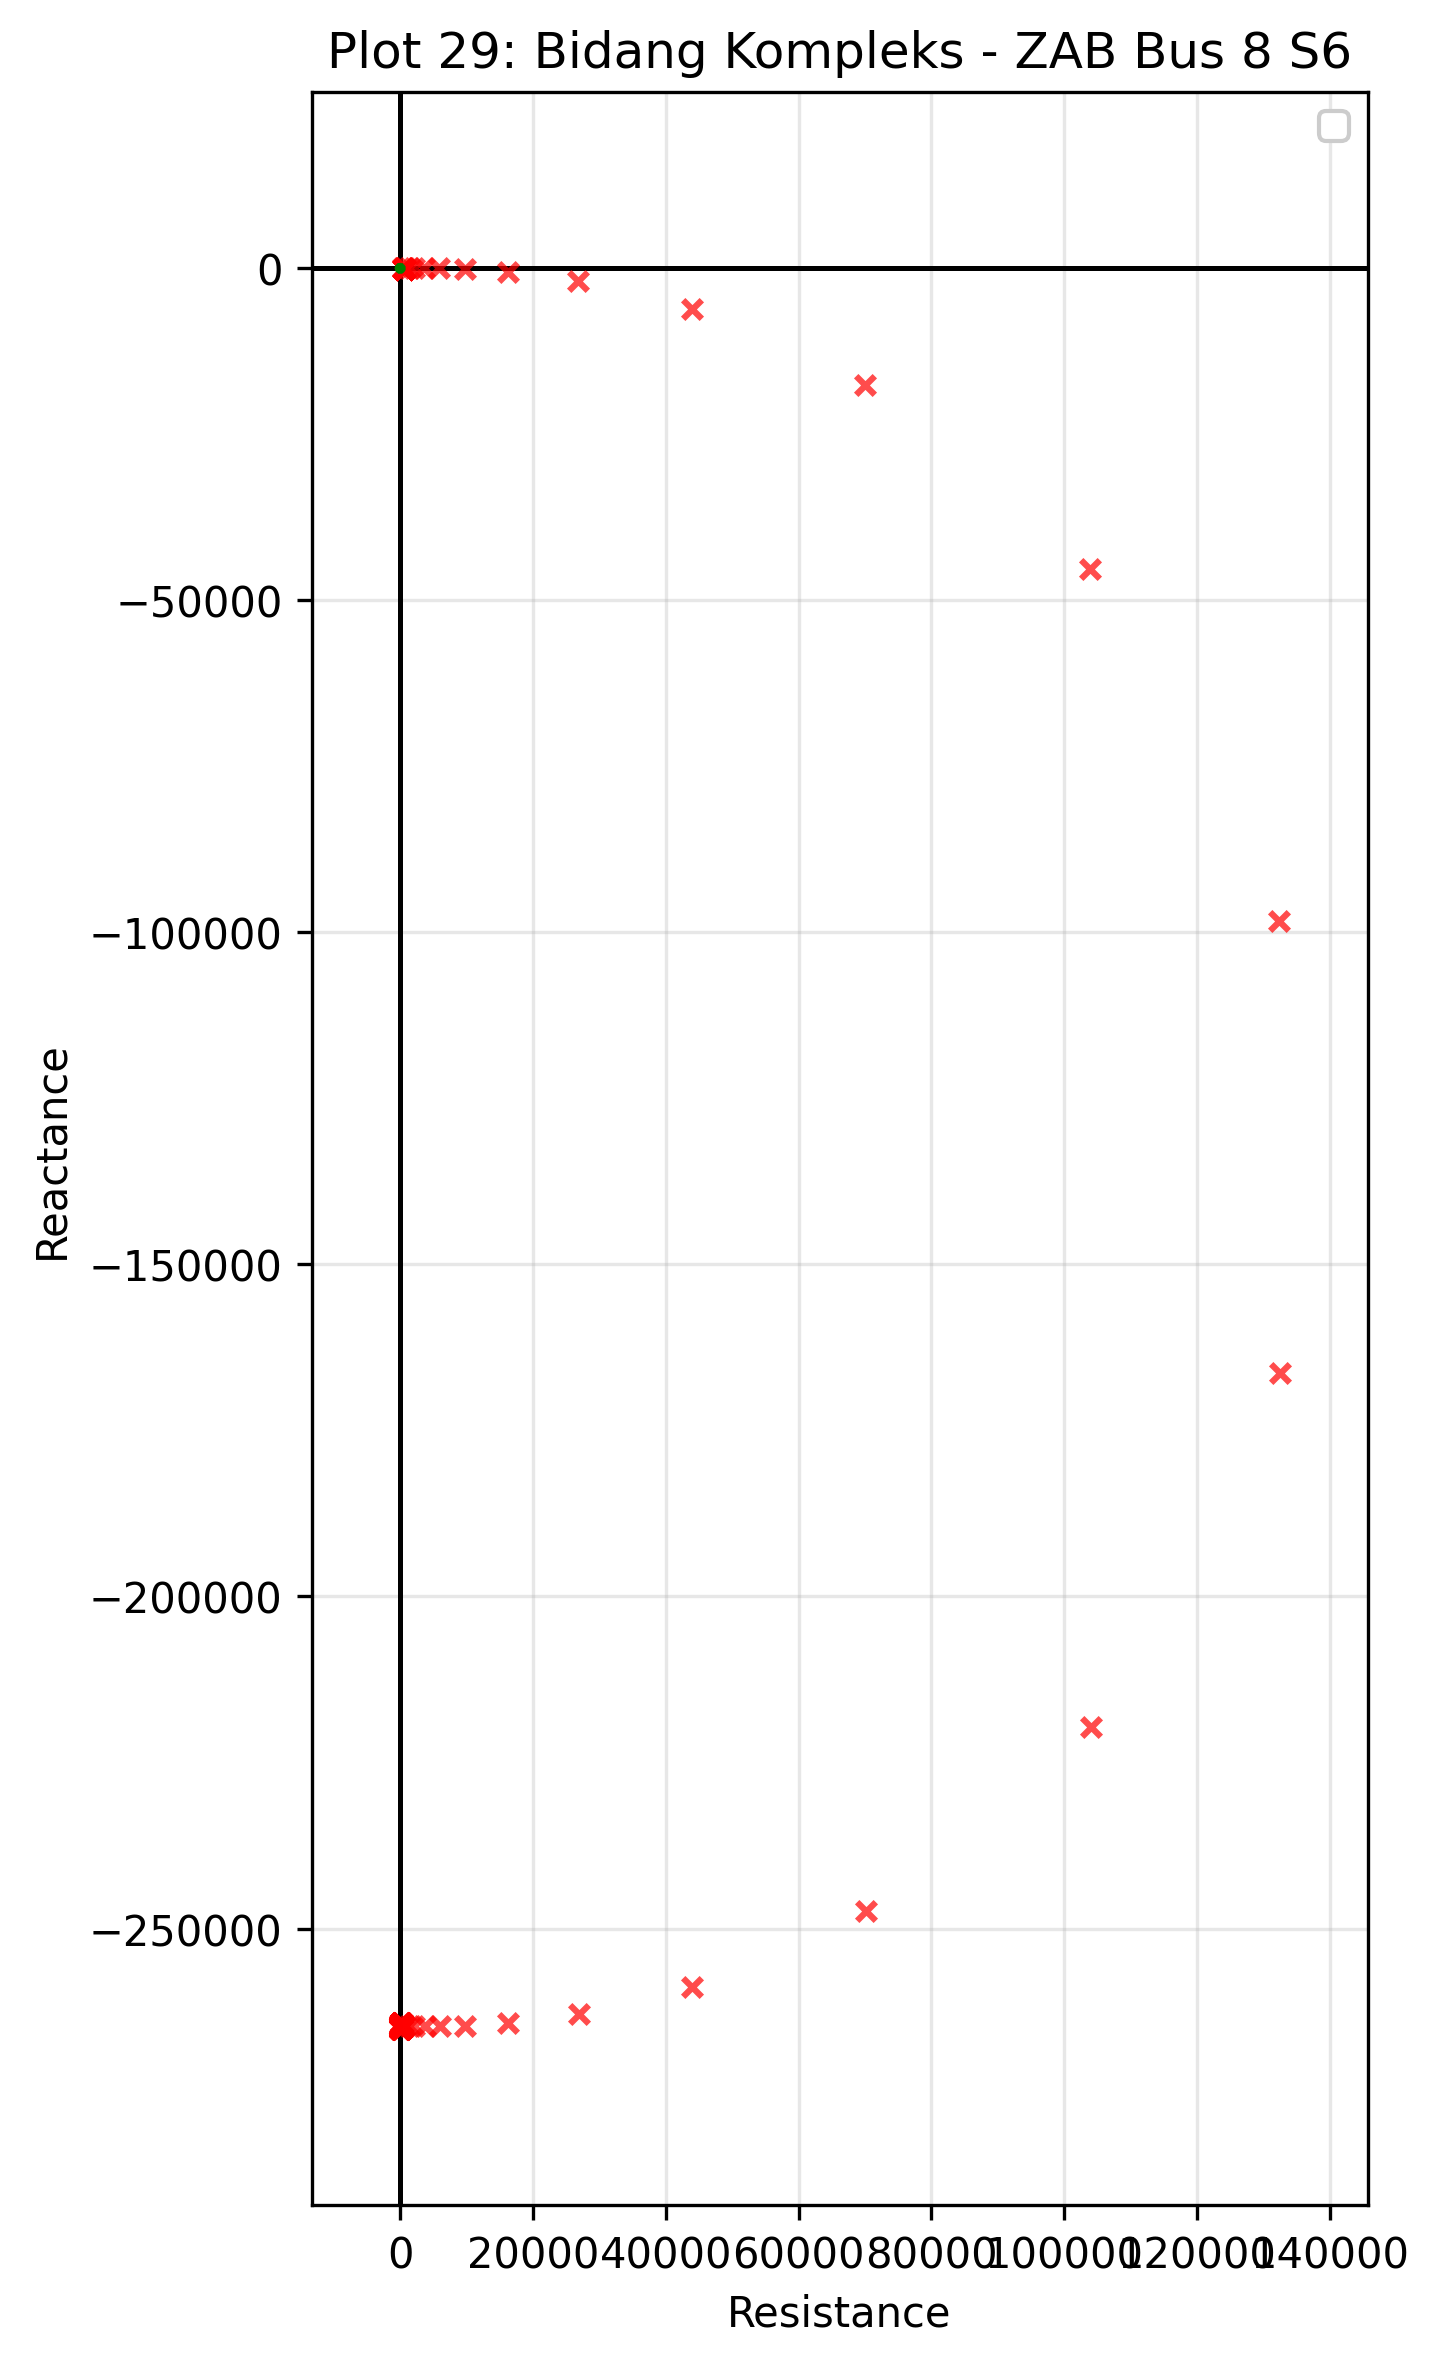
\includegraphics[width=0.8\textwidth]{contents/chapter-4/PRIA_29_ZAB_Bus_8_S6.png}
%     \caption{Impedansi Tampak ZAB Bus 8 Skenario 6}
%     \label{fig:PRIA_29_ZAB_Bus_8_S6}
% \end{figure}

% \begin{figure}[H]
%     \centering
%     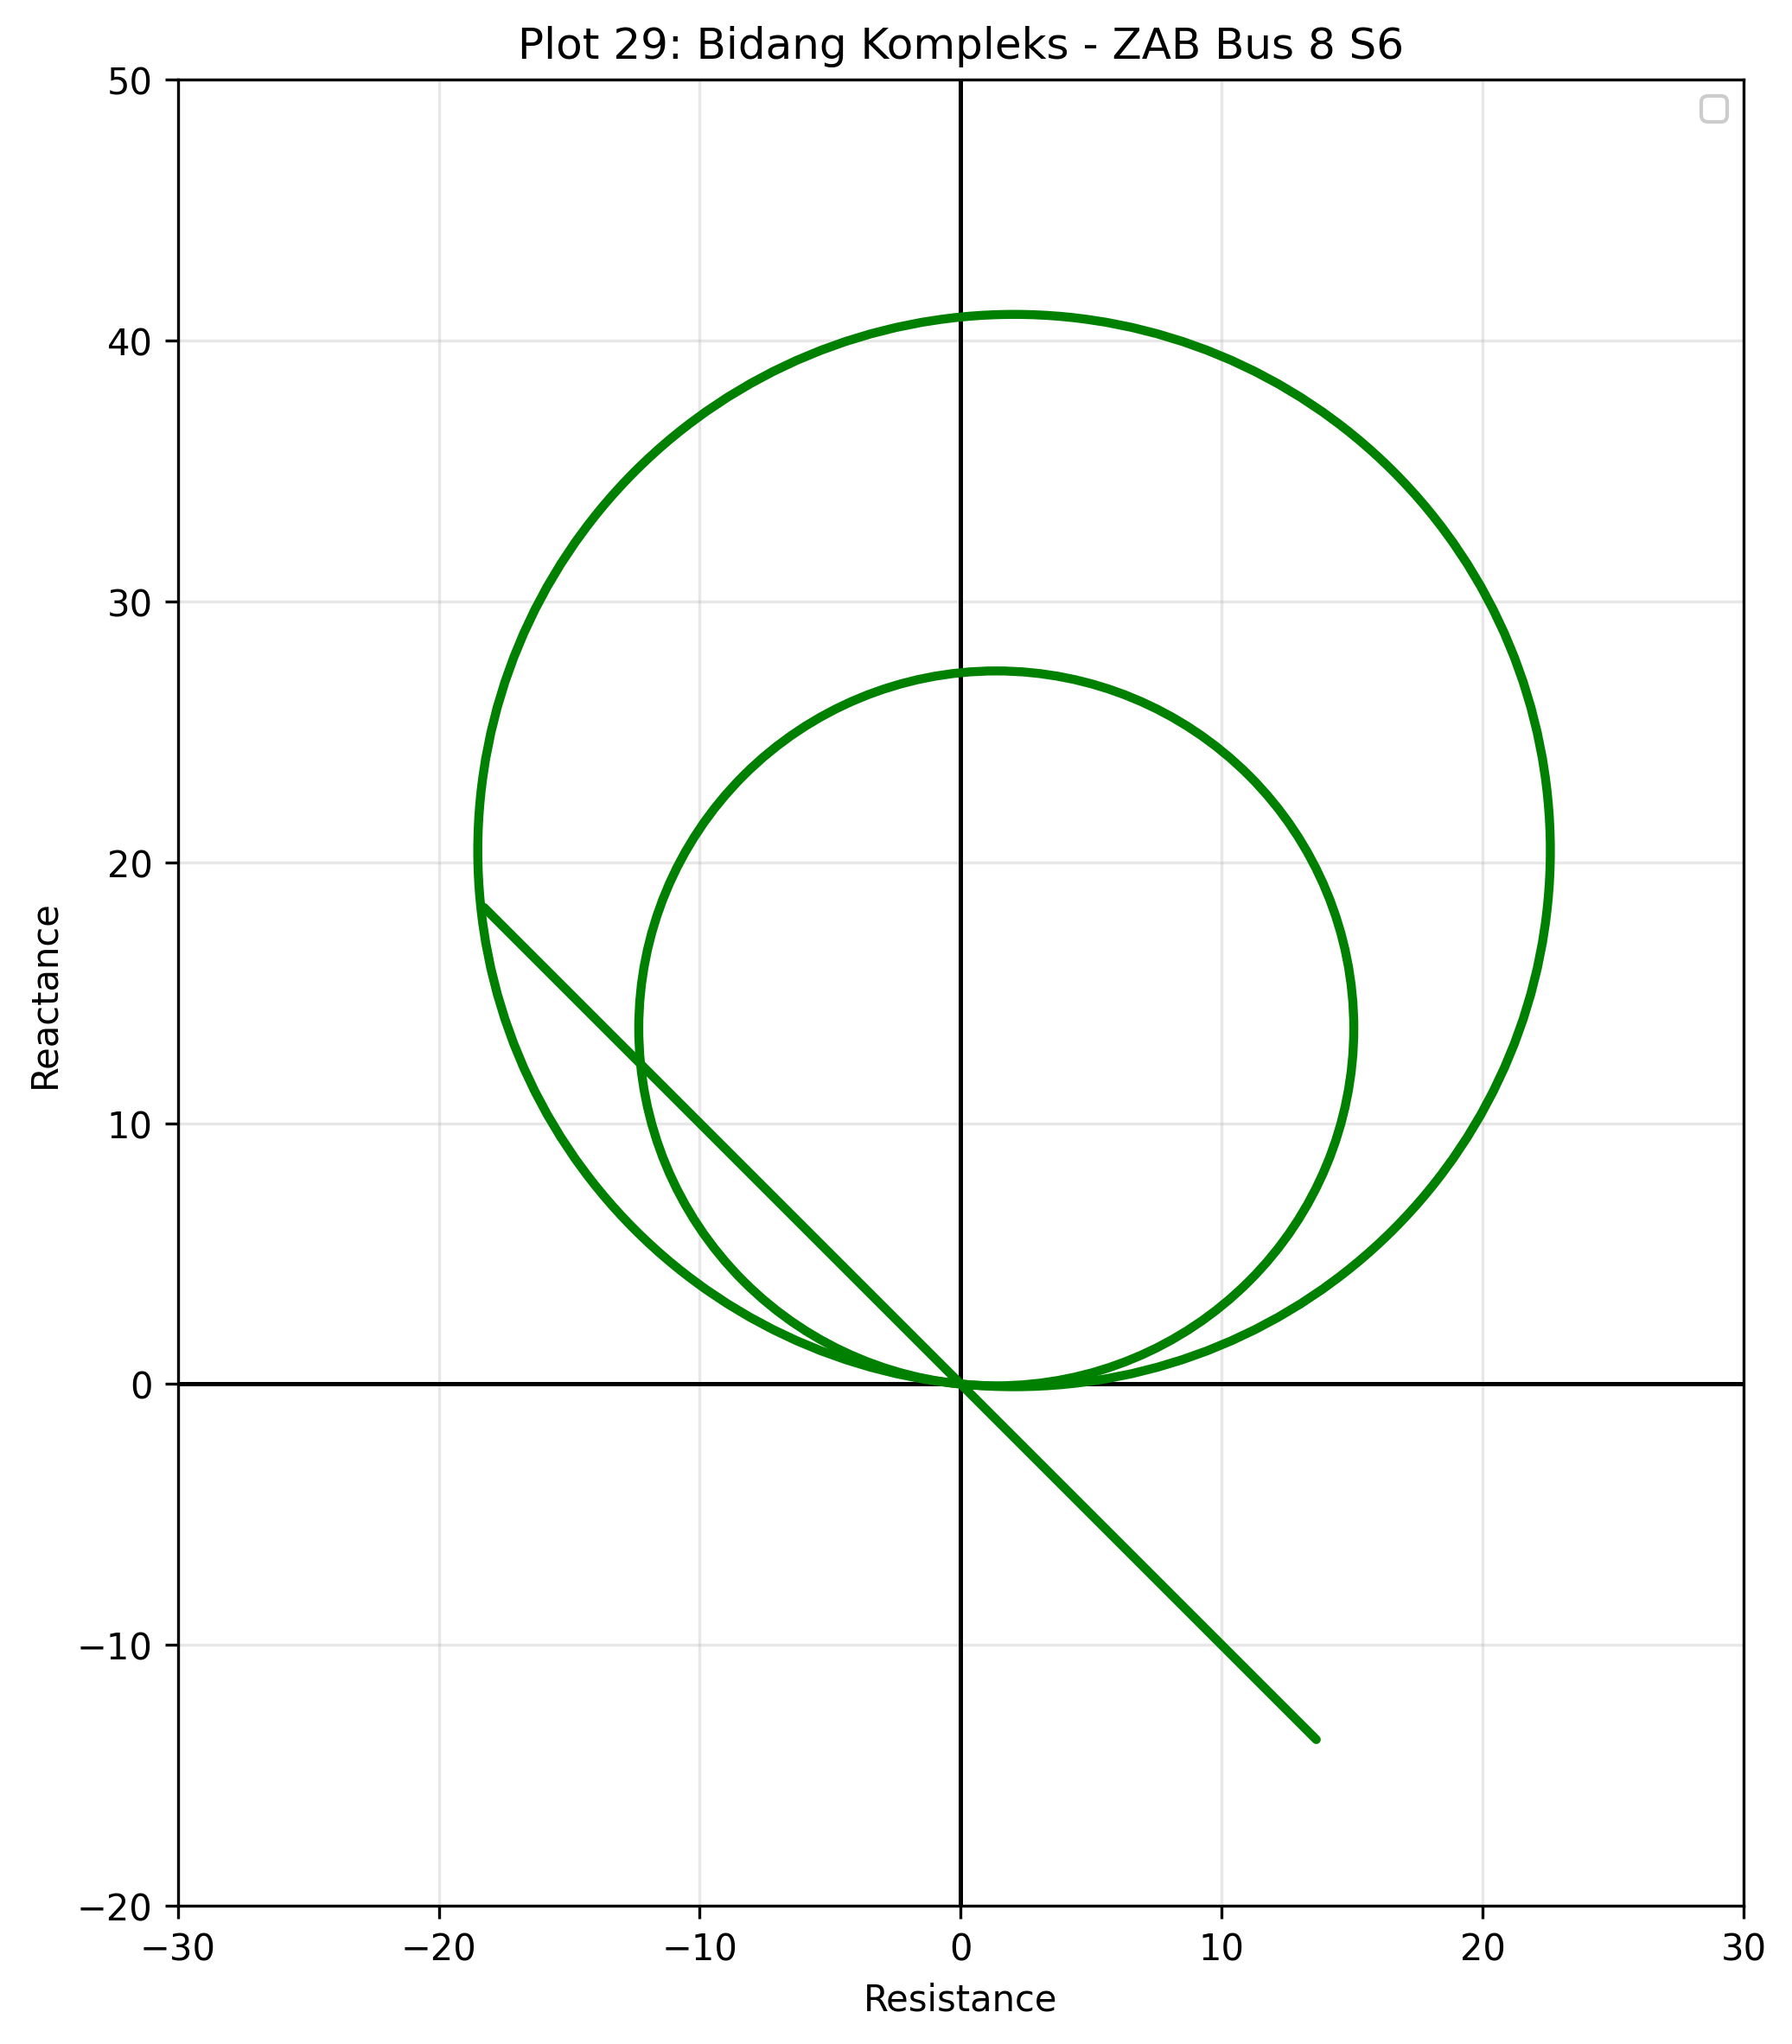
\includegraphics[width=0.8\textwidth]{contents/chapter-4/PRIZI_29_ZAB_Bus_8_S6.png}
%     \caption{Impedansi Tampak ZAB Bus 8 Skenario 6}
%     \label{fig:PRIZI_29_ZAB_Bus_8_S6}
% \end{figure}

\begin{figure}[H]
    \centering

    % Gambar sebelah kiri
    \begin{subfigure}[t]{0.48\textwidth}
        \centering
        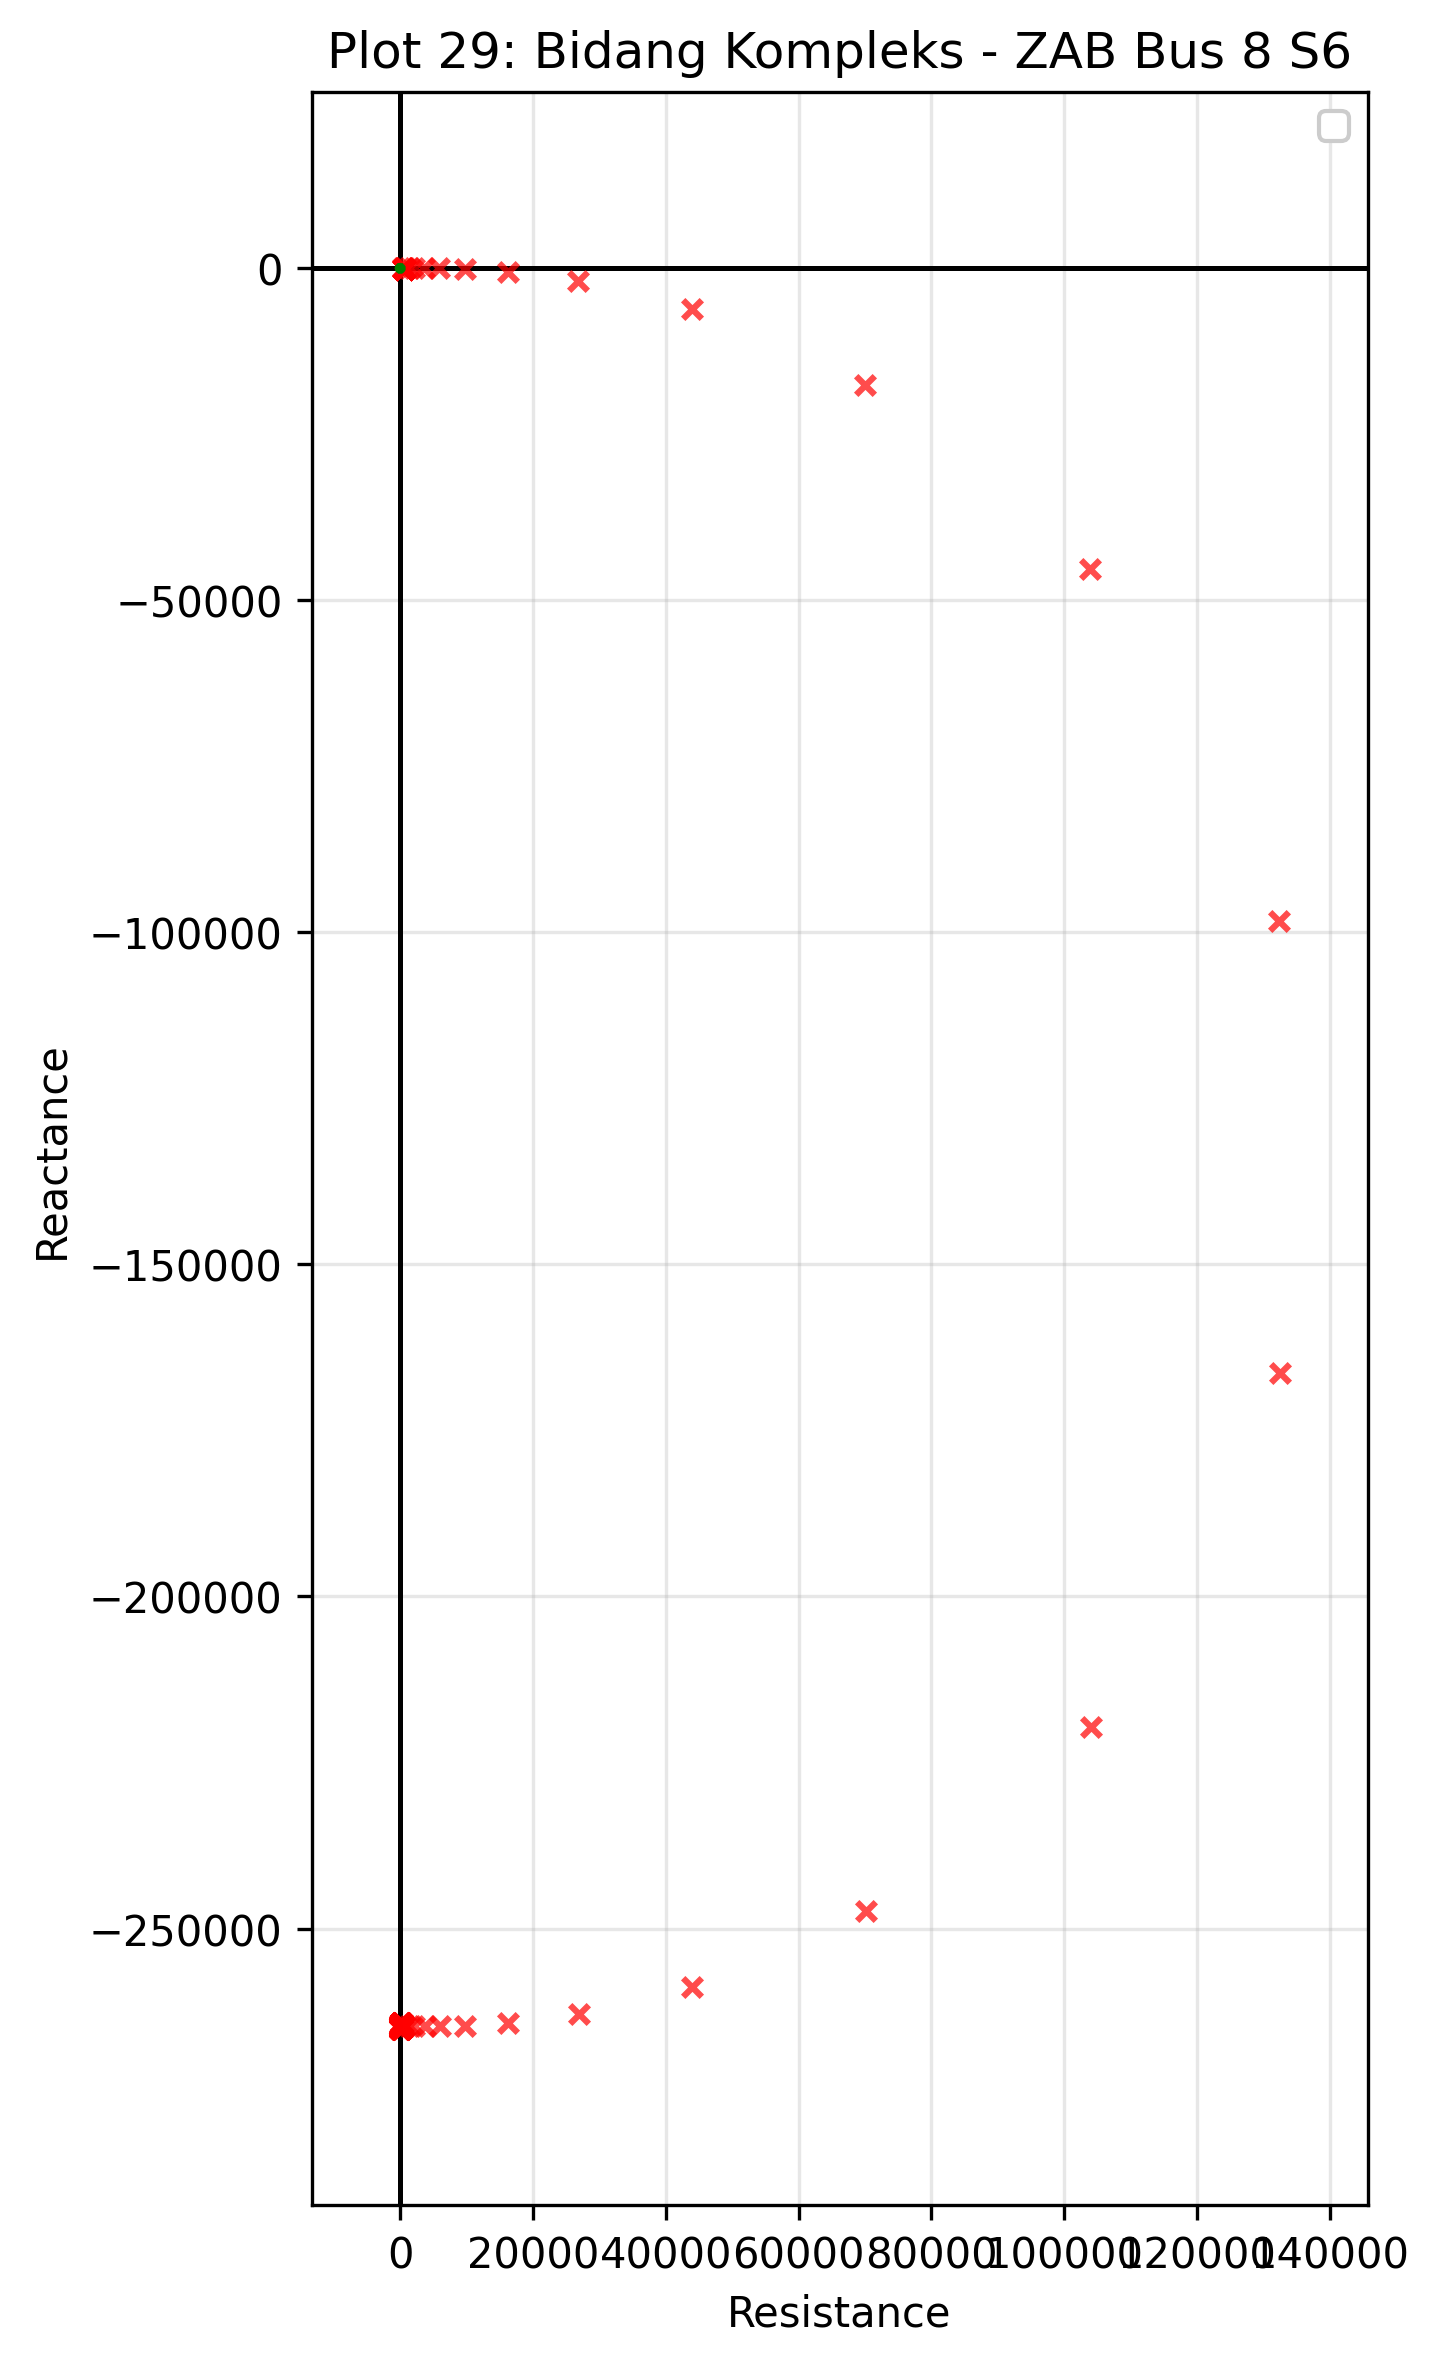
\includegraphics[width=\textwidth]{contents/chapter-4/PRIA_29_ZAB_Bus_8_S6.png}
        \caption{Seluruh Impedansi Tampak}
        \label{fig:PRIA_29_ZAB_Bus_8_S6}
    \end{subfigure}
    \hfill
    % Gambar sebelah kanan
    \begin{subfigure}[t]{0.48\textwidth}
        \centering
        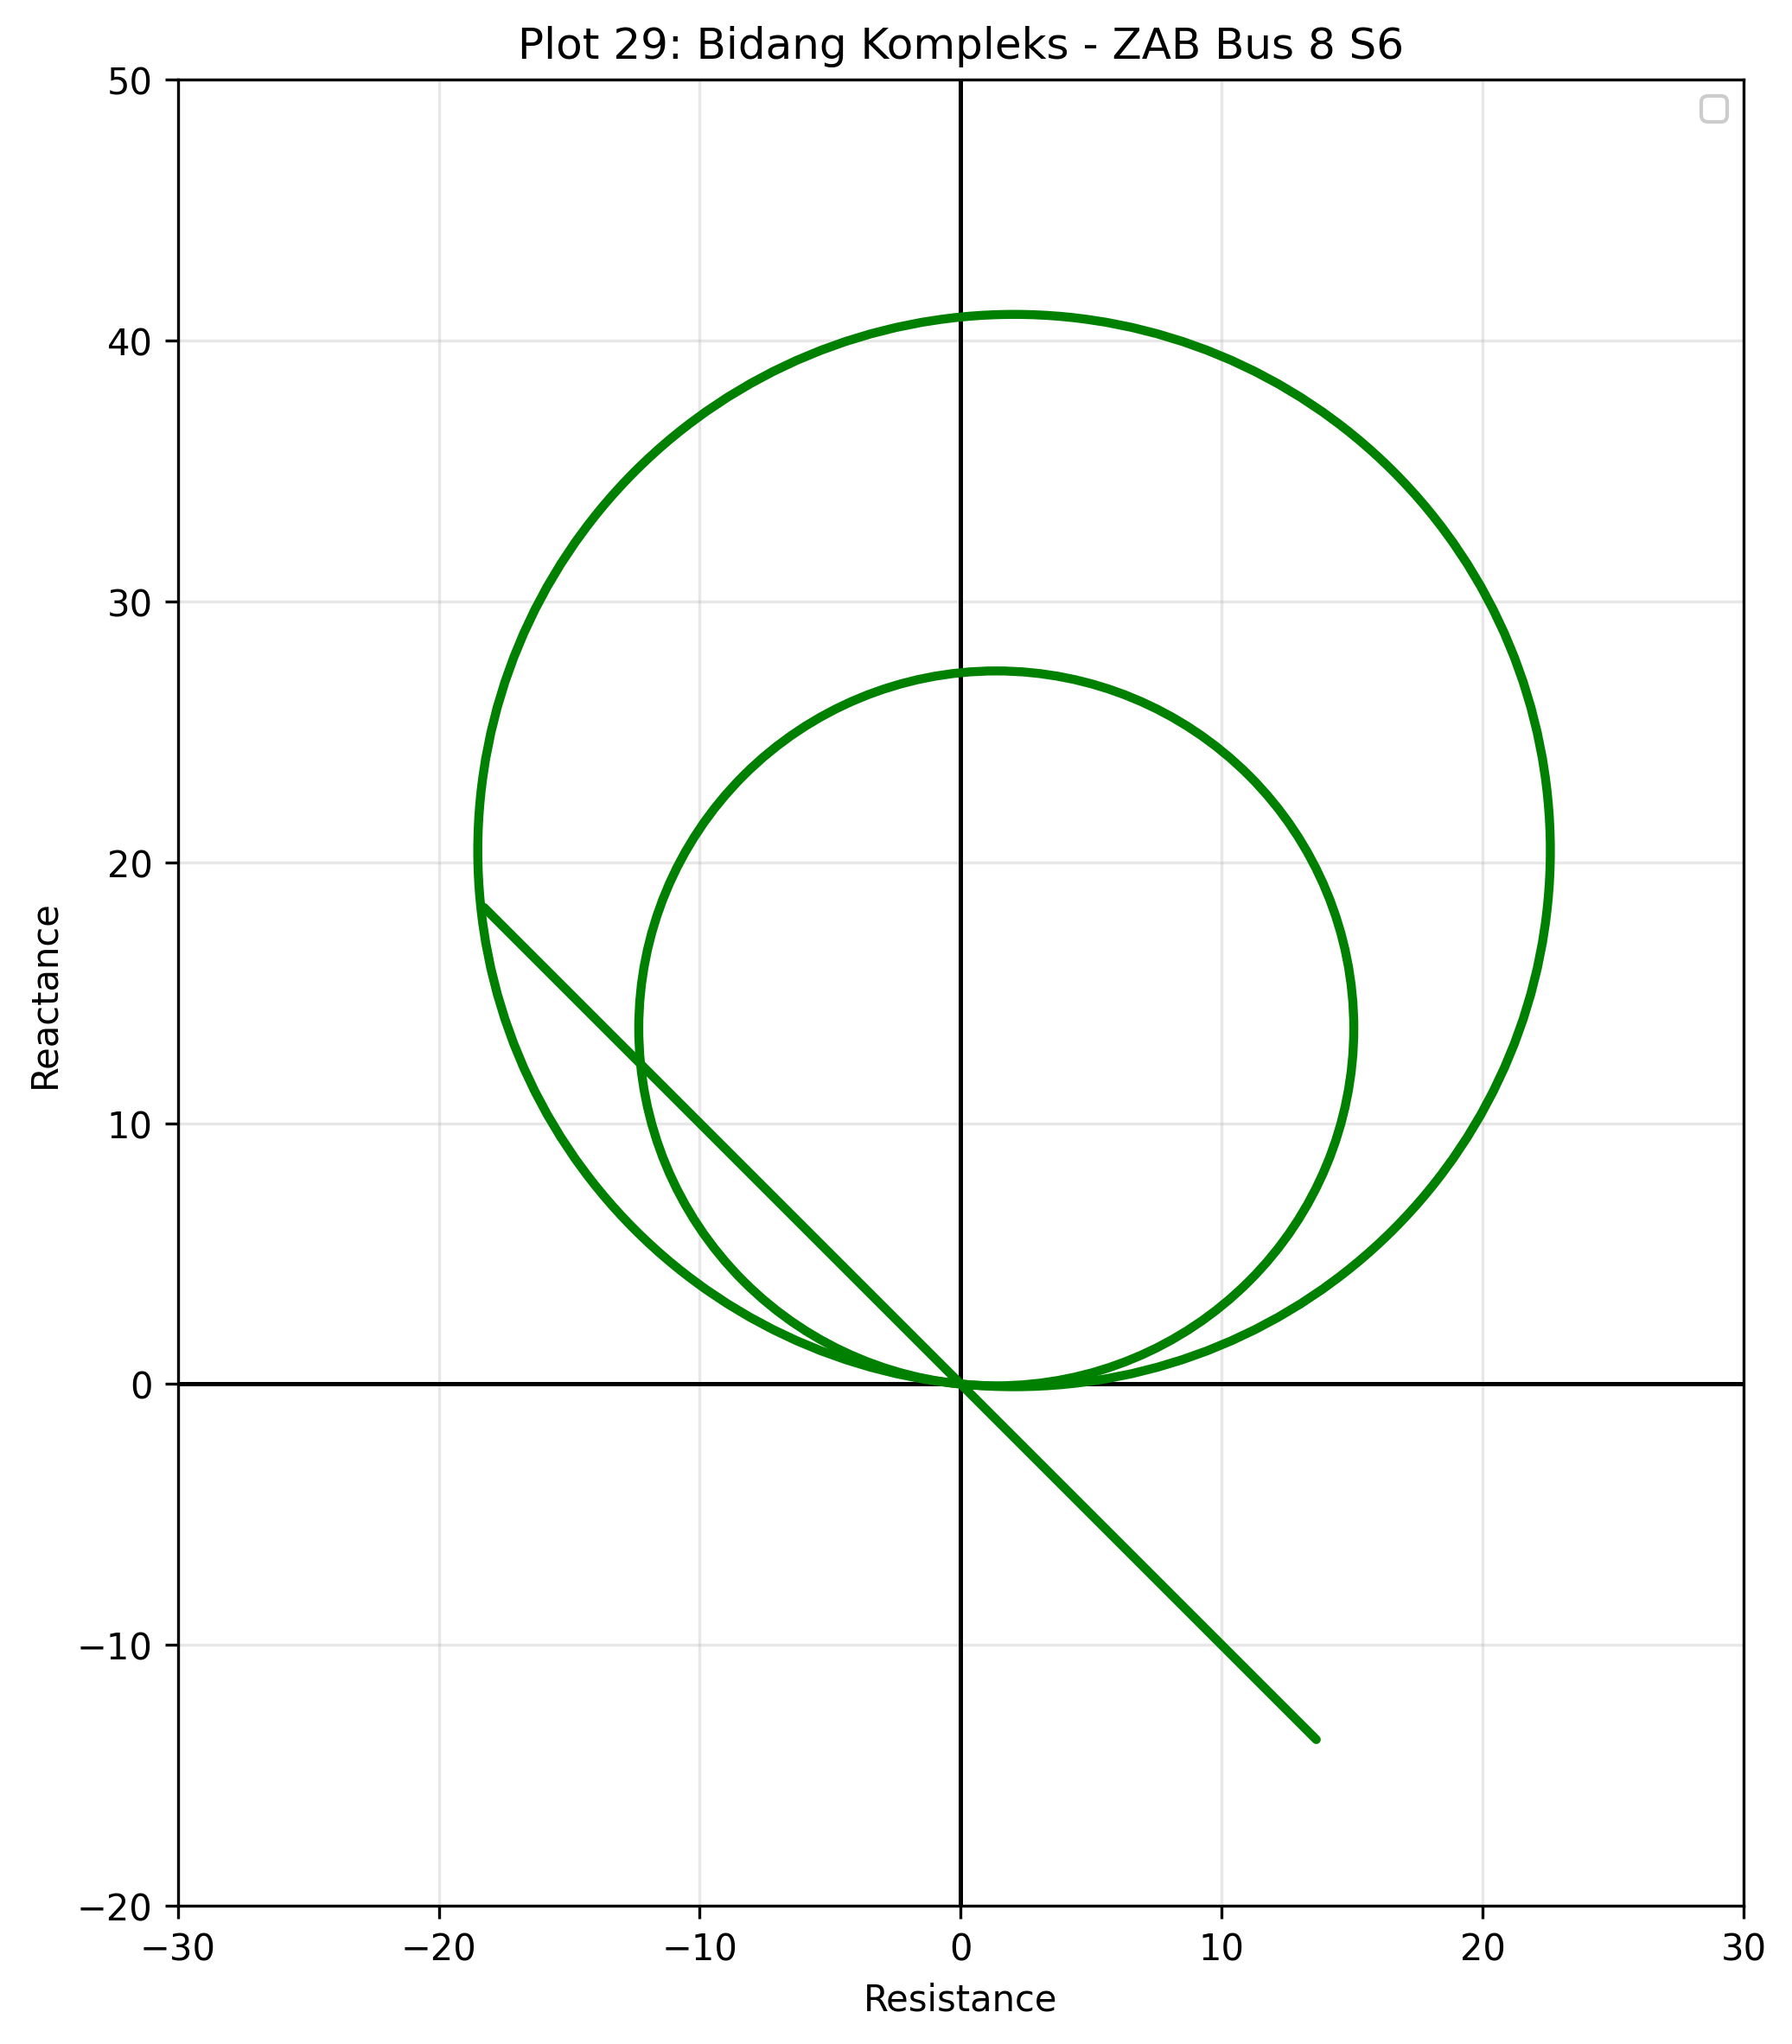
\includegraphics[width=\textwidth]{contents/chapter-4/PRIZI_29_ZAB_Bus_8_S6.png}
        \caption{Zoom In Pada Zona Proteksi}
        \label{fig:PRIZI_29_ZAB_Bus_8_S6}
    \end{subfigure}

    \caption{Impedansi Tampak ZAB Bus 8 Skenario 6}
    \label{fig:Impedansi_Tampak_ZAB_Bus_8_S6}
\end{figure}

Gambar \ref{fig:Impedansi_Tampak_ZAB_Bus_8_S6} menunjukkan bahwa impedansi tampak loop fasa A dengan fasa B yang dibaca oleh relay 21 sisi Bus 8 tidak masuk ke dalam zona proteksi. Sama seperti dua elemen sebelumnya, kondisi ini berkaitan dengan arus sekunder CT pada Gambar \ref{fig:Bus_8_Ex_DLG_S6} yang belum memenuhi syarat \textit{starting} untuk membuat relay aktif. Dengan demikian, berdasarkan acuan gangguan eksternal DLG pada Subbab \ref{subsec:tanpa_IBR_ex_dlg}, respons relay 21 sisi Bus 8 pada skenario 6 menunjukkan \textit{misoperation}.


%%%%%%%%%%%%%%%%%%%%%%%%%%%%%%%%%%%%%%%%%%%%%%%%%%%%%%%%%%%%%%

% \begin{figure}[H]
%     \centering
%     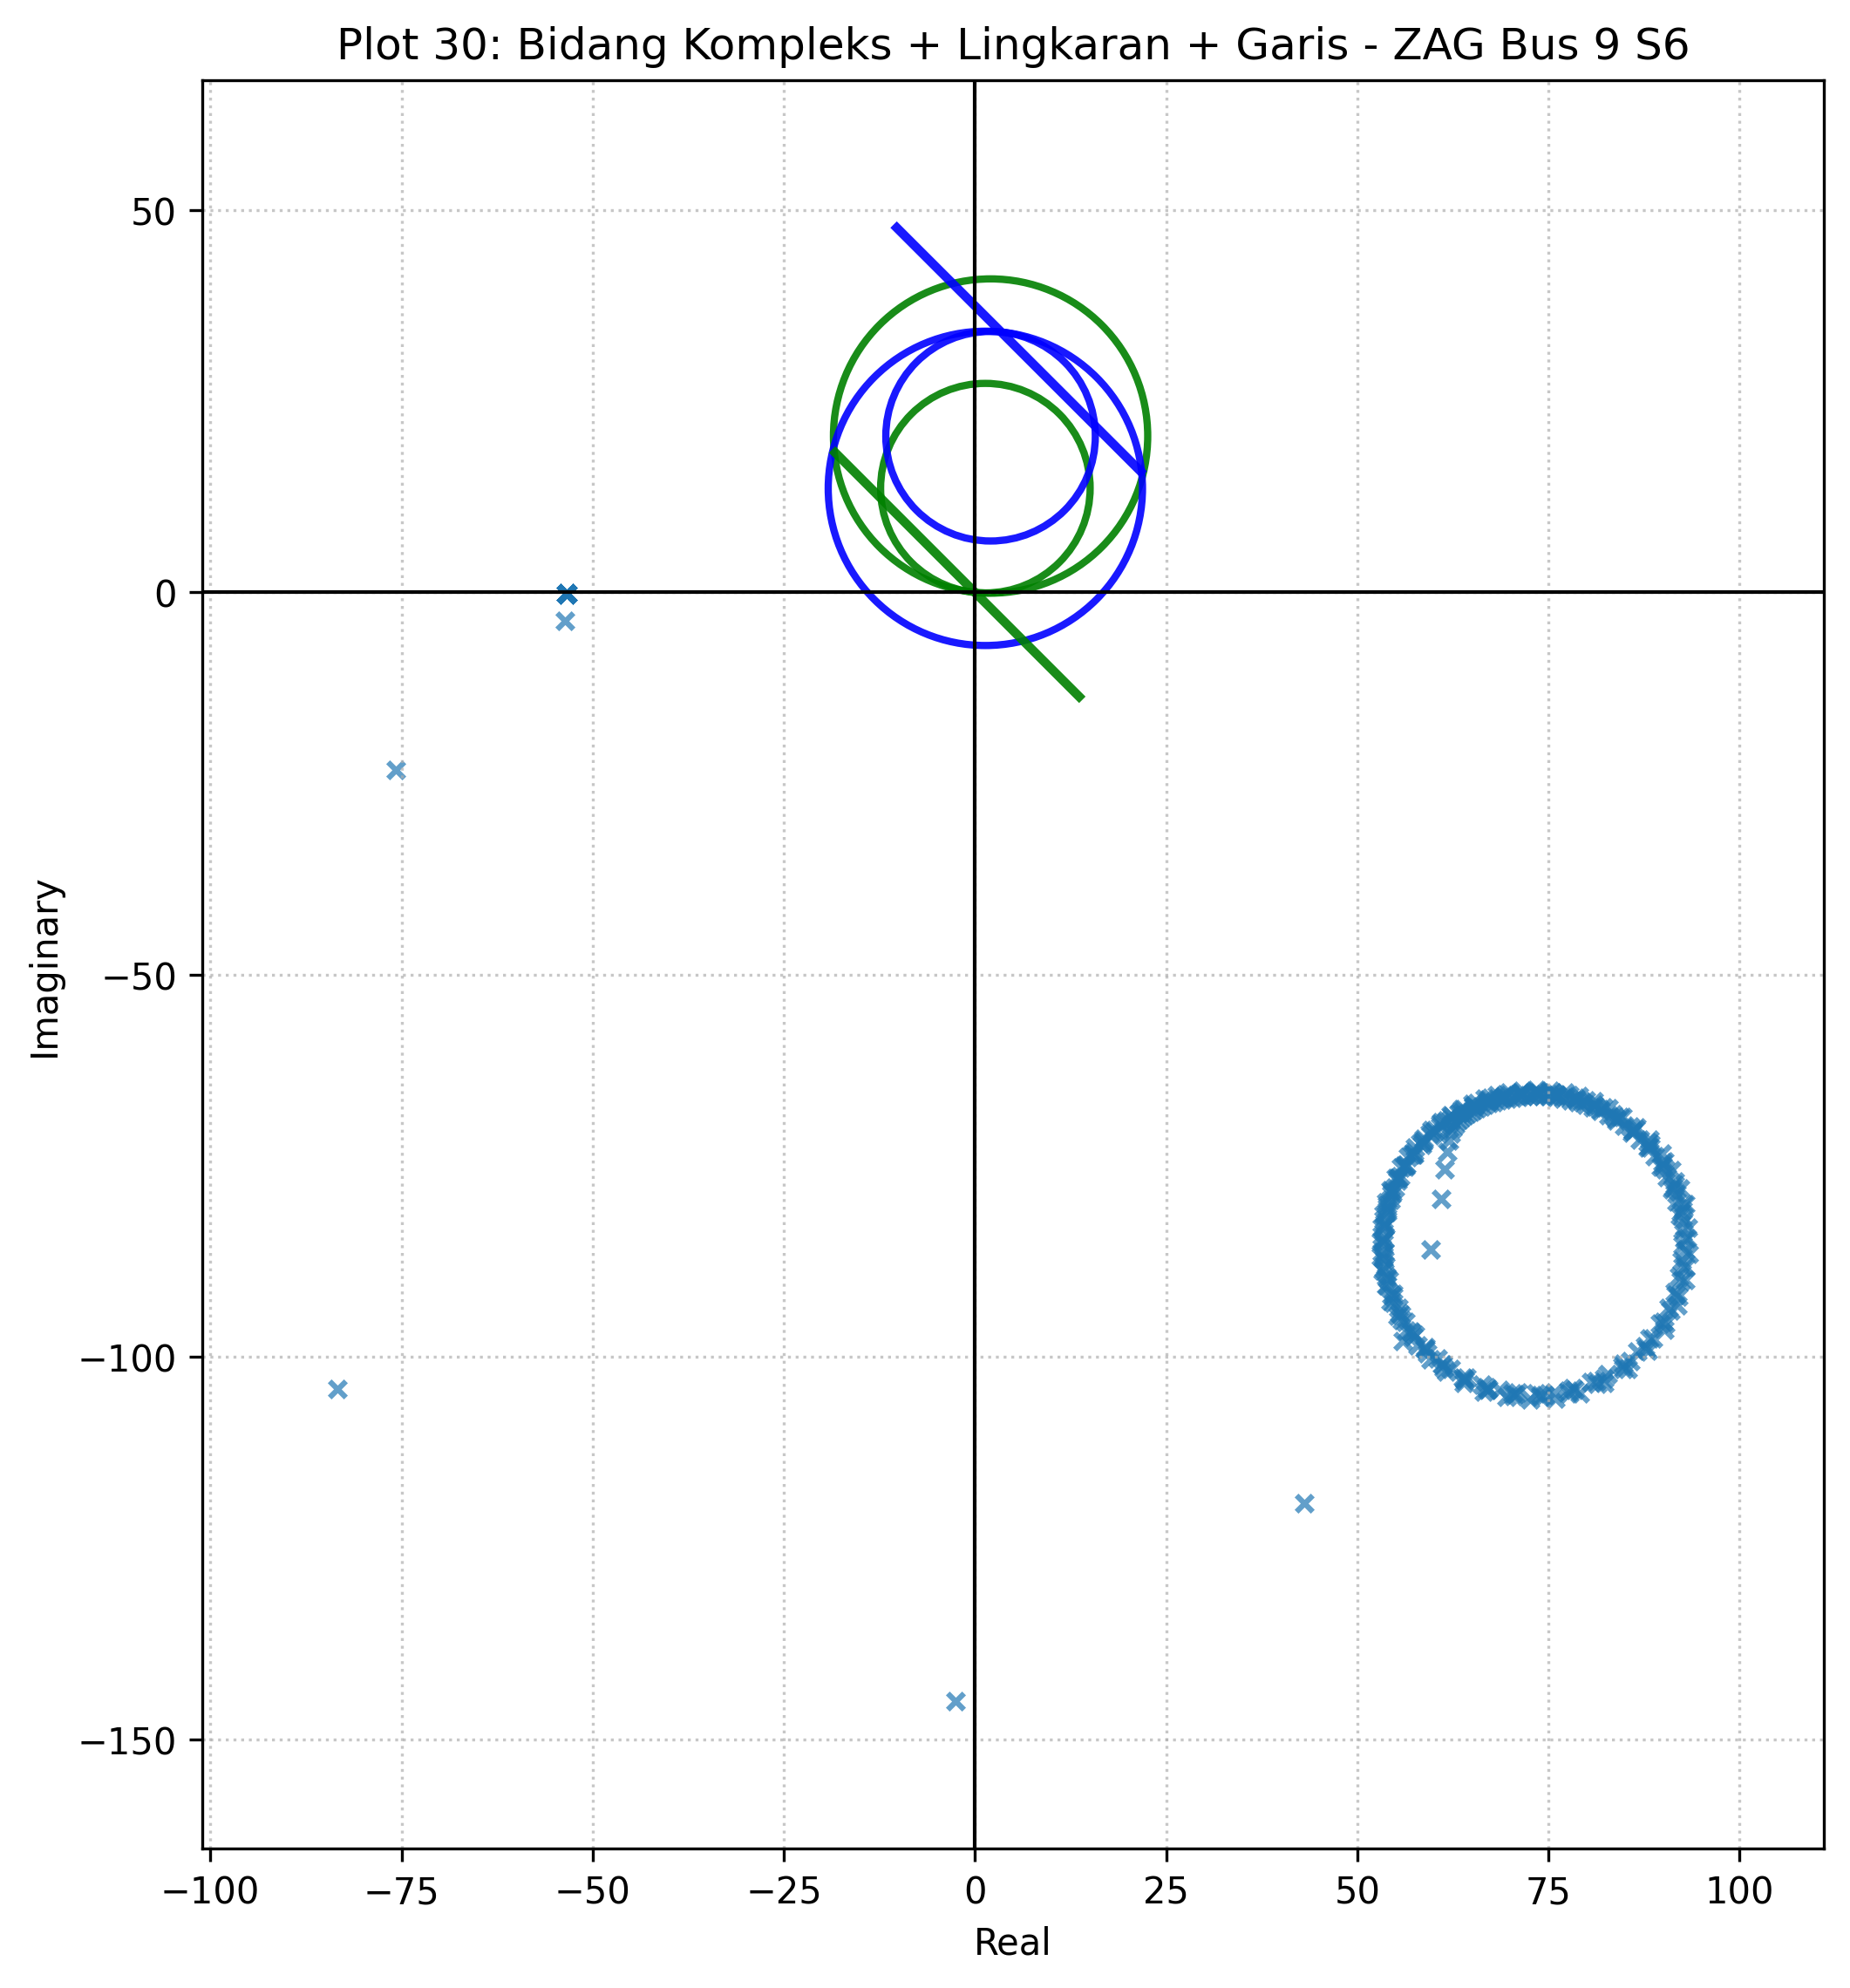
\includegraphics[width=0.8\textwidth]{contents/chapter-4/30_ZAG_Bus_9_S6_dengan_lingkaran_dan_garis.png}
%     \caption{Impedansi Tampak ZAG Bus 9 Skenario 6}
%     \label{fig:30_ZAG_Bus_9_S6_dengan_lingkaran_dan_garis}
% \end{figure}

%%%%%%%%%%%%%%%%%%%%%%%%%%%%%%%%%SISI PRIMER%%%%%%%%%%%%%%%%%%%%%%%%%%%%%%%%%%

% \begin{figure}[H]
%     \centering
%     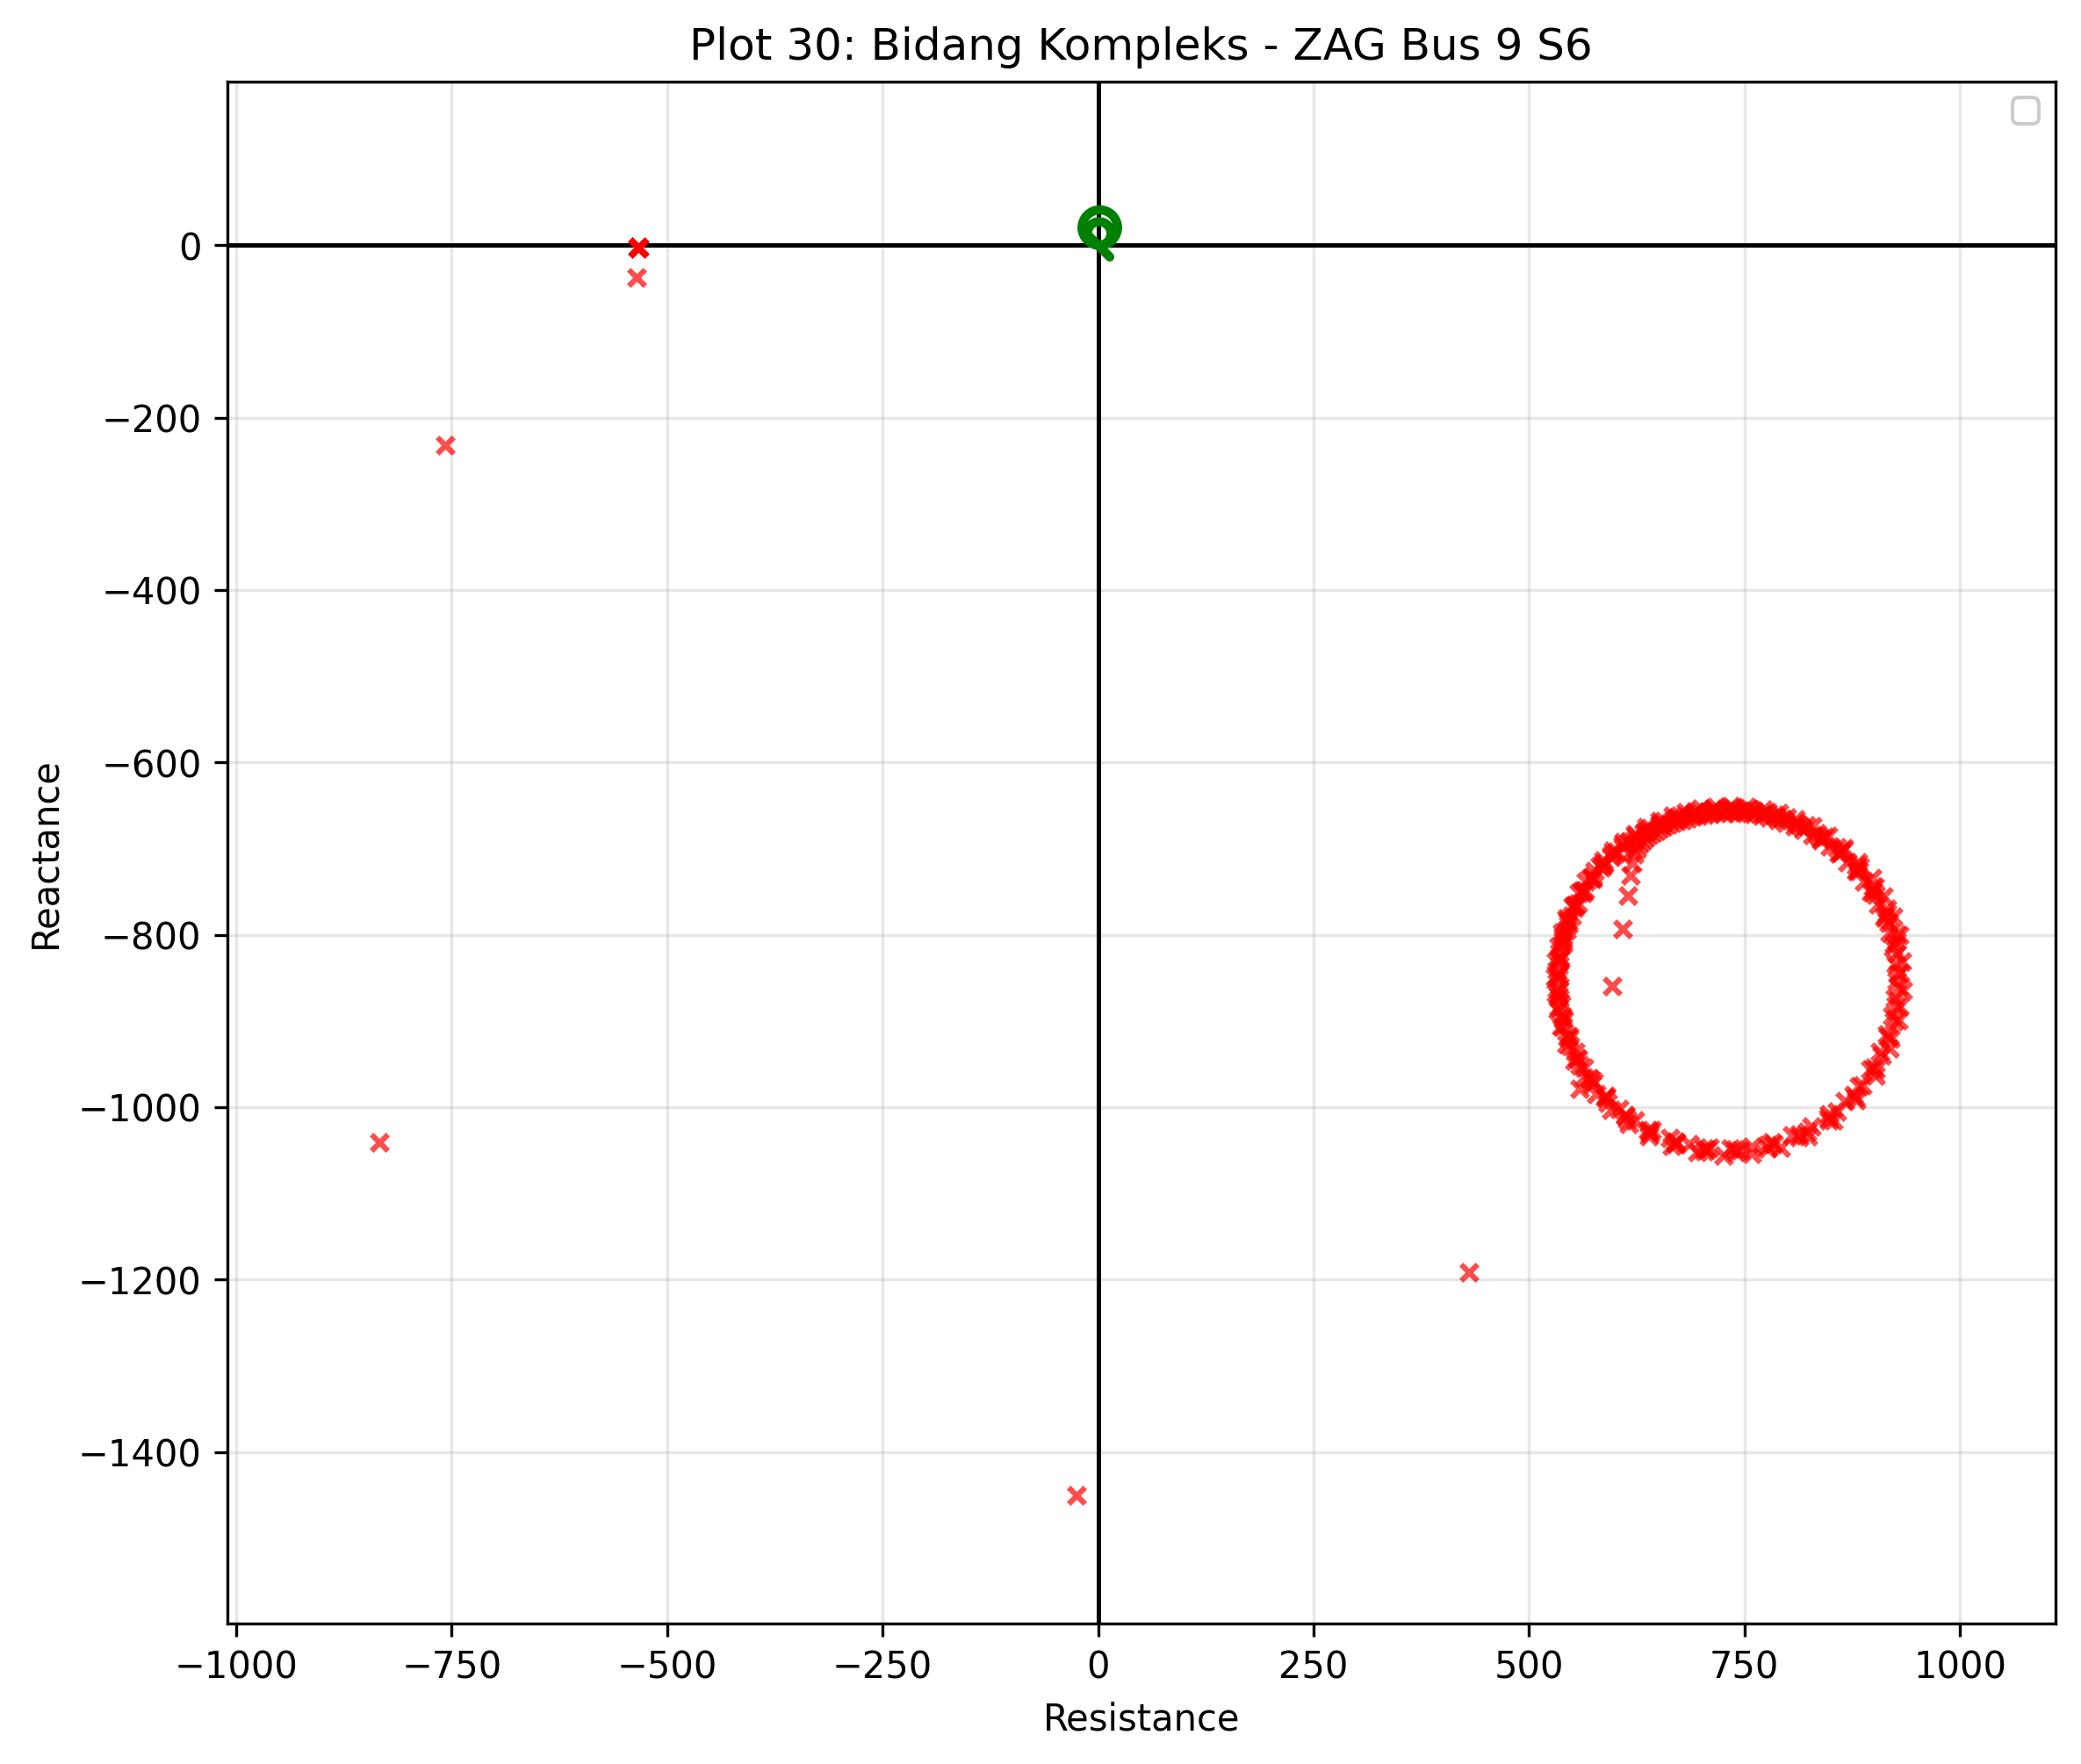
\includegraphics[width=0.8\textwidth]{contents/chapter-4/PRIA_30_ZAG_Bus_9_S6.png}
%     \caption{Impedansi Tampak ZAG Bus 9 Skenario 6}
%     \label{fig:PRIA_30_ZAG_Bus_9_S6}
% \end{figure}

% \begin{figure}[H]
%     \centering
%     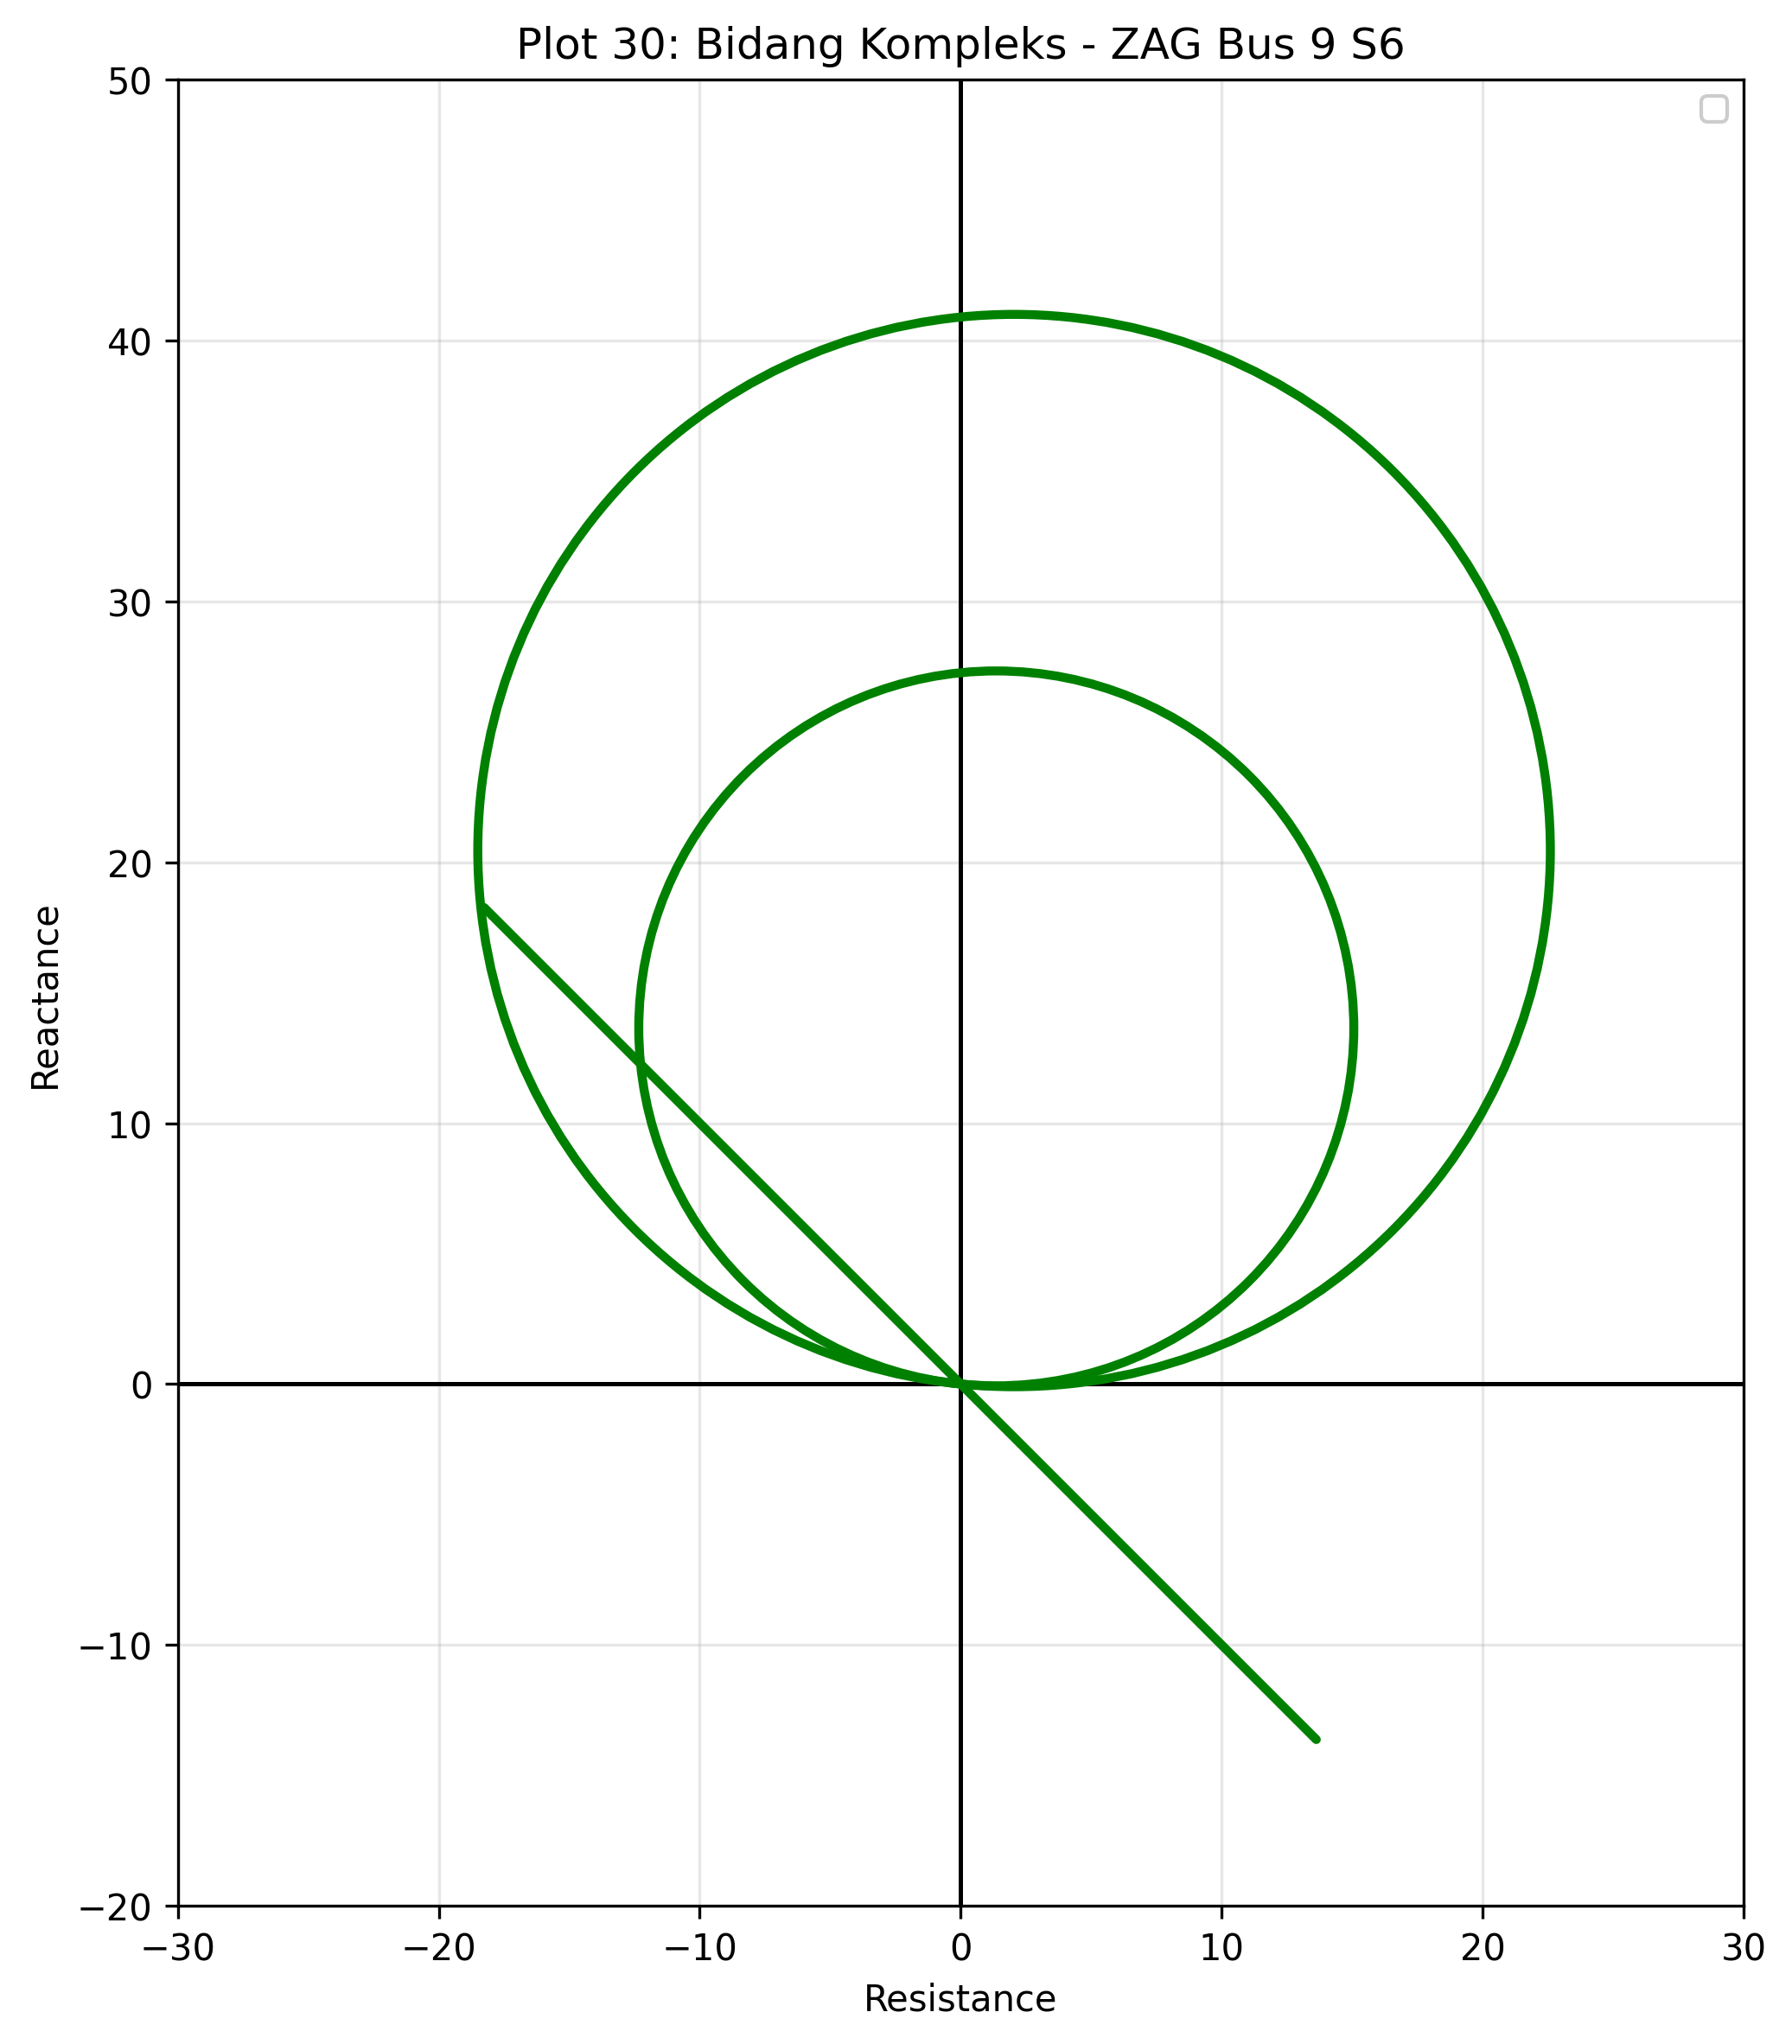
\includegraphics[width=0.8\textwidth]{contents/chapter-4/PRIZI_30_ZAG_Bus_9_S6.png}
%     \caption{Impedansi Tampak ZAG Bus 9 Skenario 6}
%     \label{fig:PRIZI_30_ZAG_Bus_9_S6}
% \end{figure}

\begin{figure}[H]
    \centering

    % Gambar sebelah kiri
    \begin{subfigure}[t]{0.48\textwidth}
        \centering
        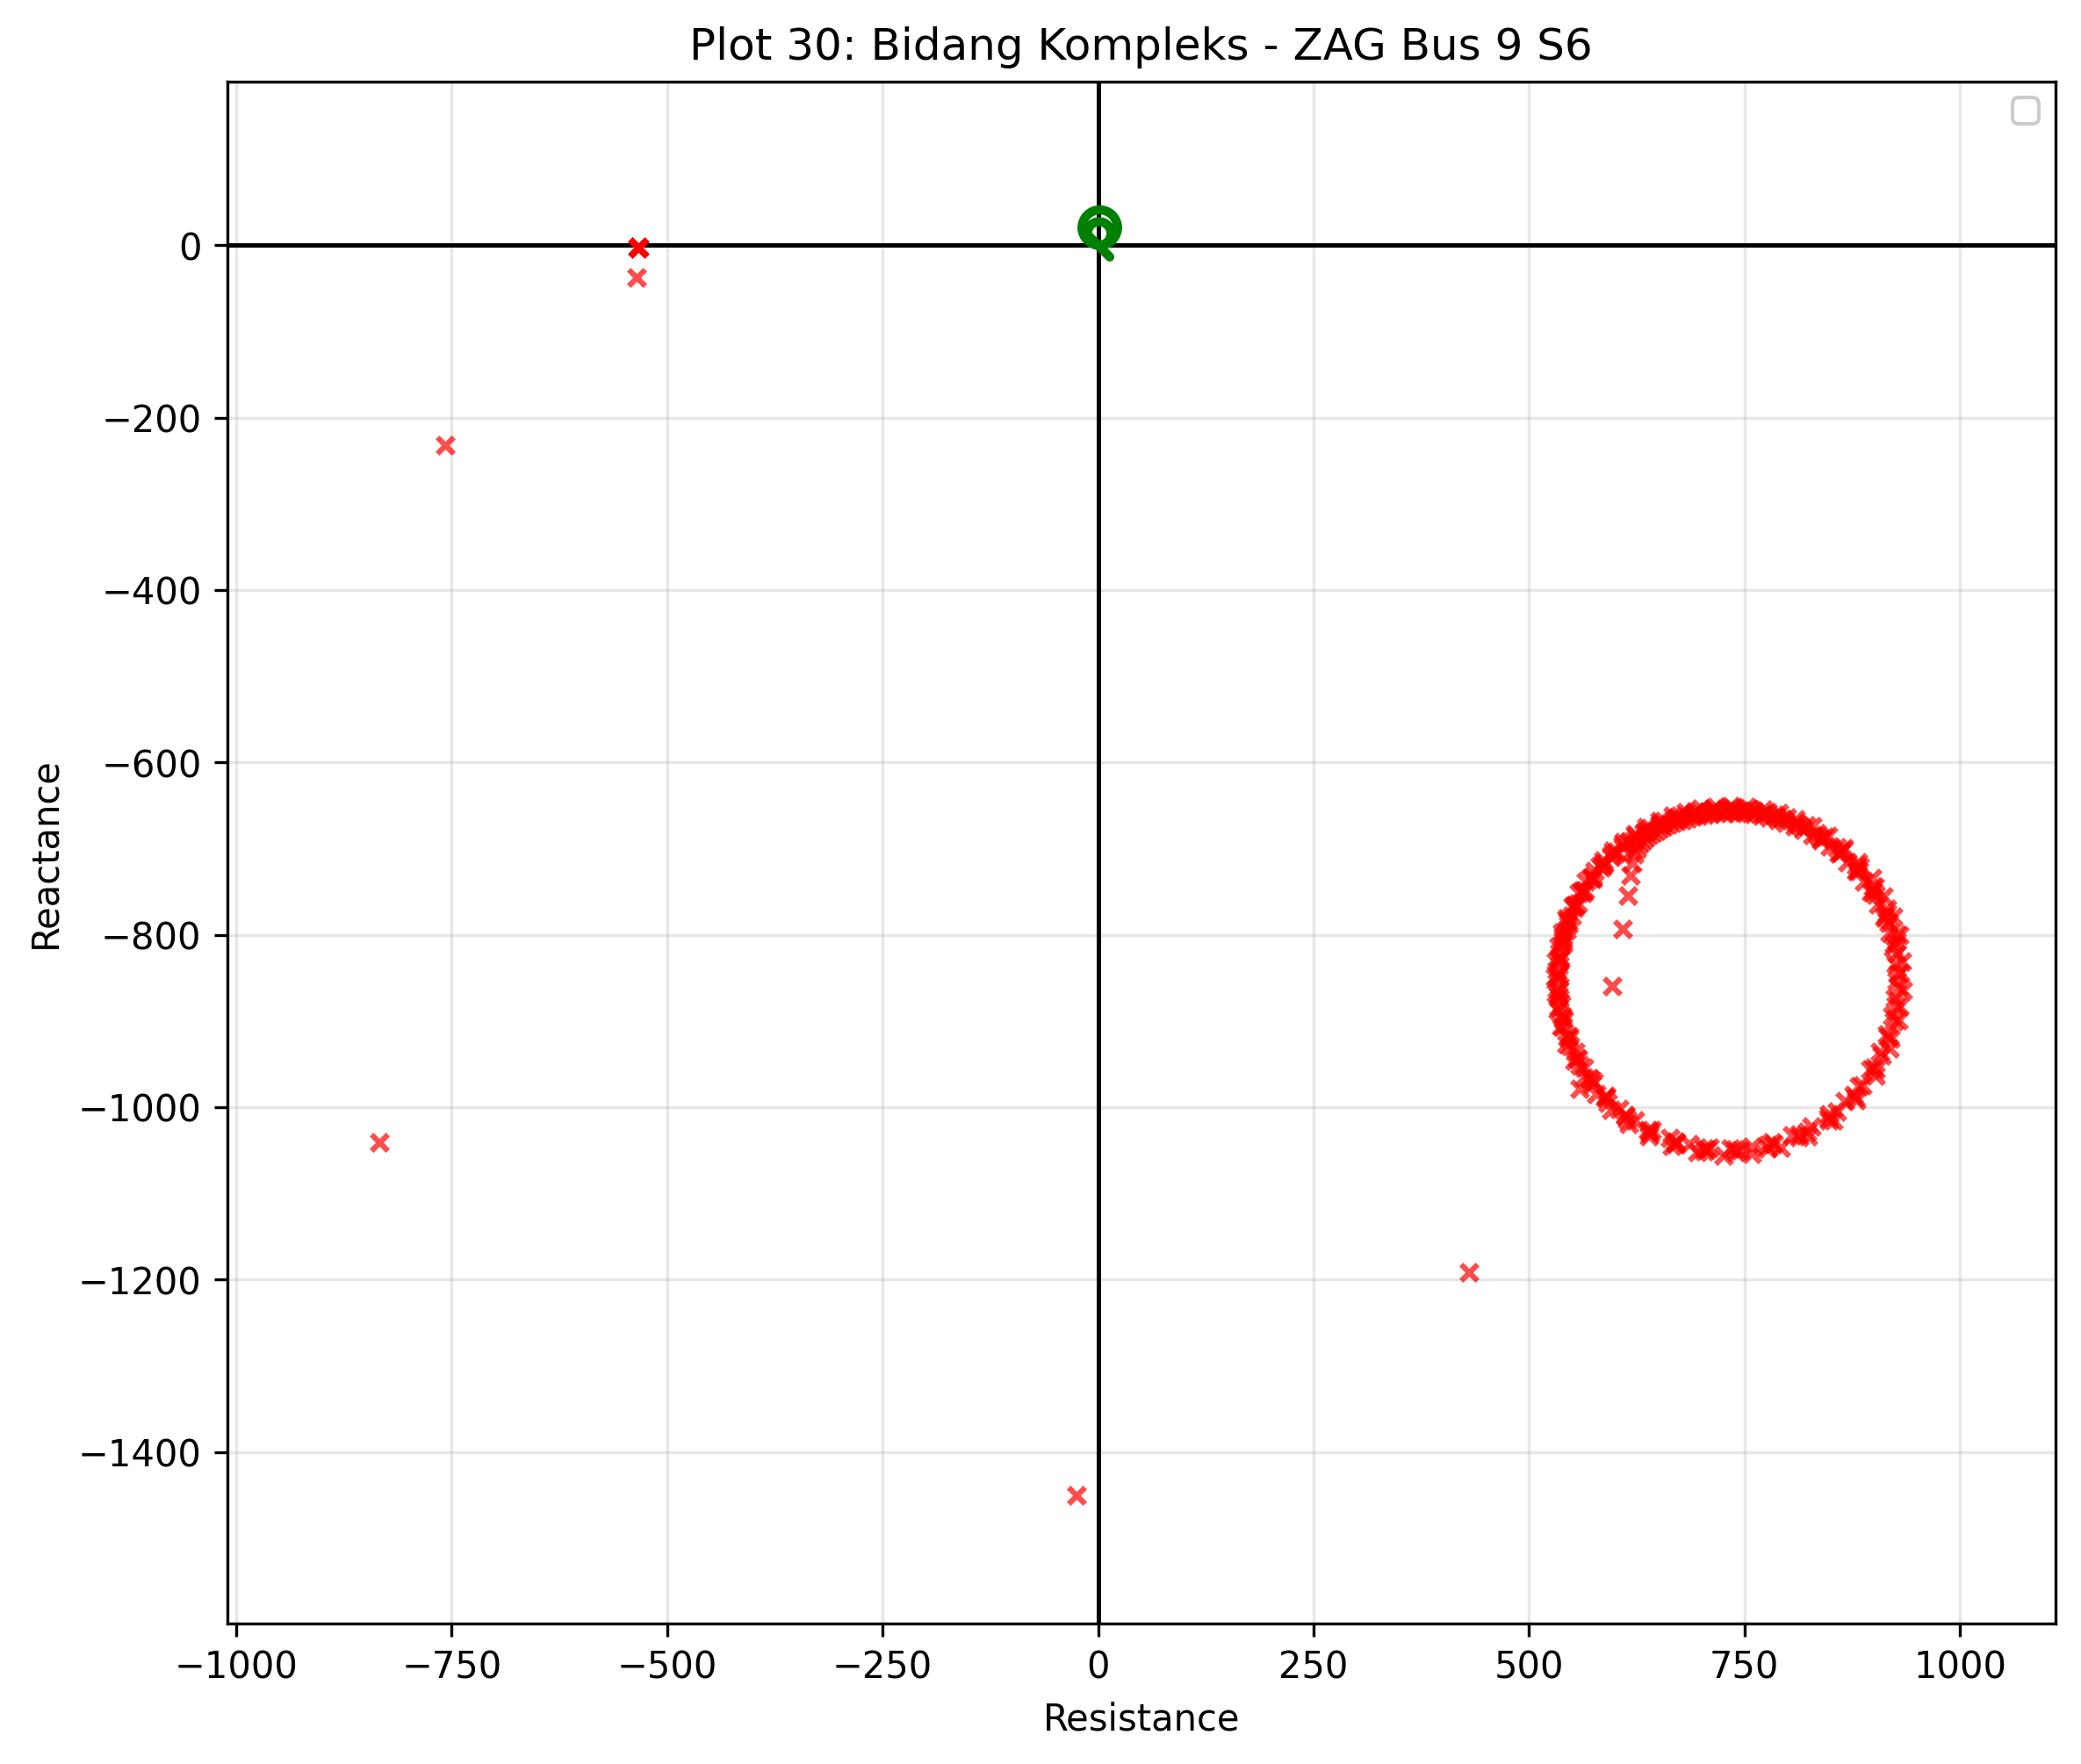
\includegraphics[width=\textwidth]{contents/chapter-4/PRIA_30_ZAG_Bus_9_S6.png}
        \caption{Seluruh Impedansi Tampak}
        \label{fig:PRIA_30_ZAG_Bus_9_S6}
    \end{subfigure}
    \hfill
    % Gambar sebelah kanan
    \begin{subfigure}[t]{0.48\textwidth}
        \centering
        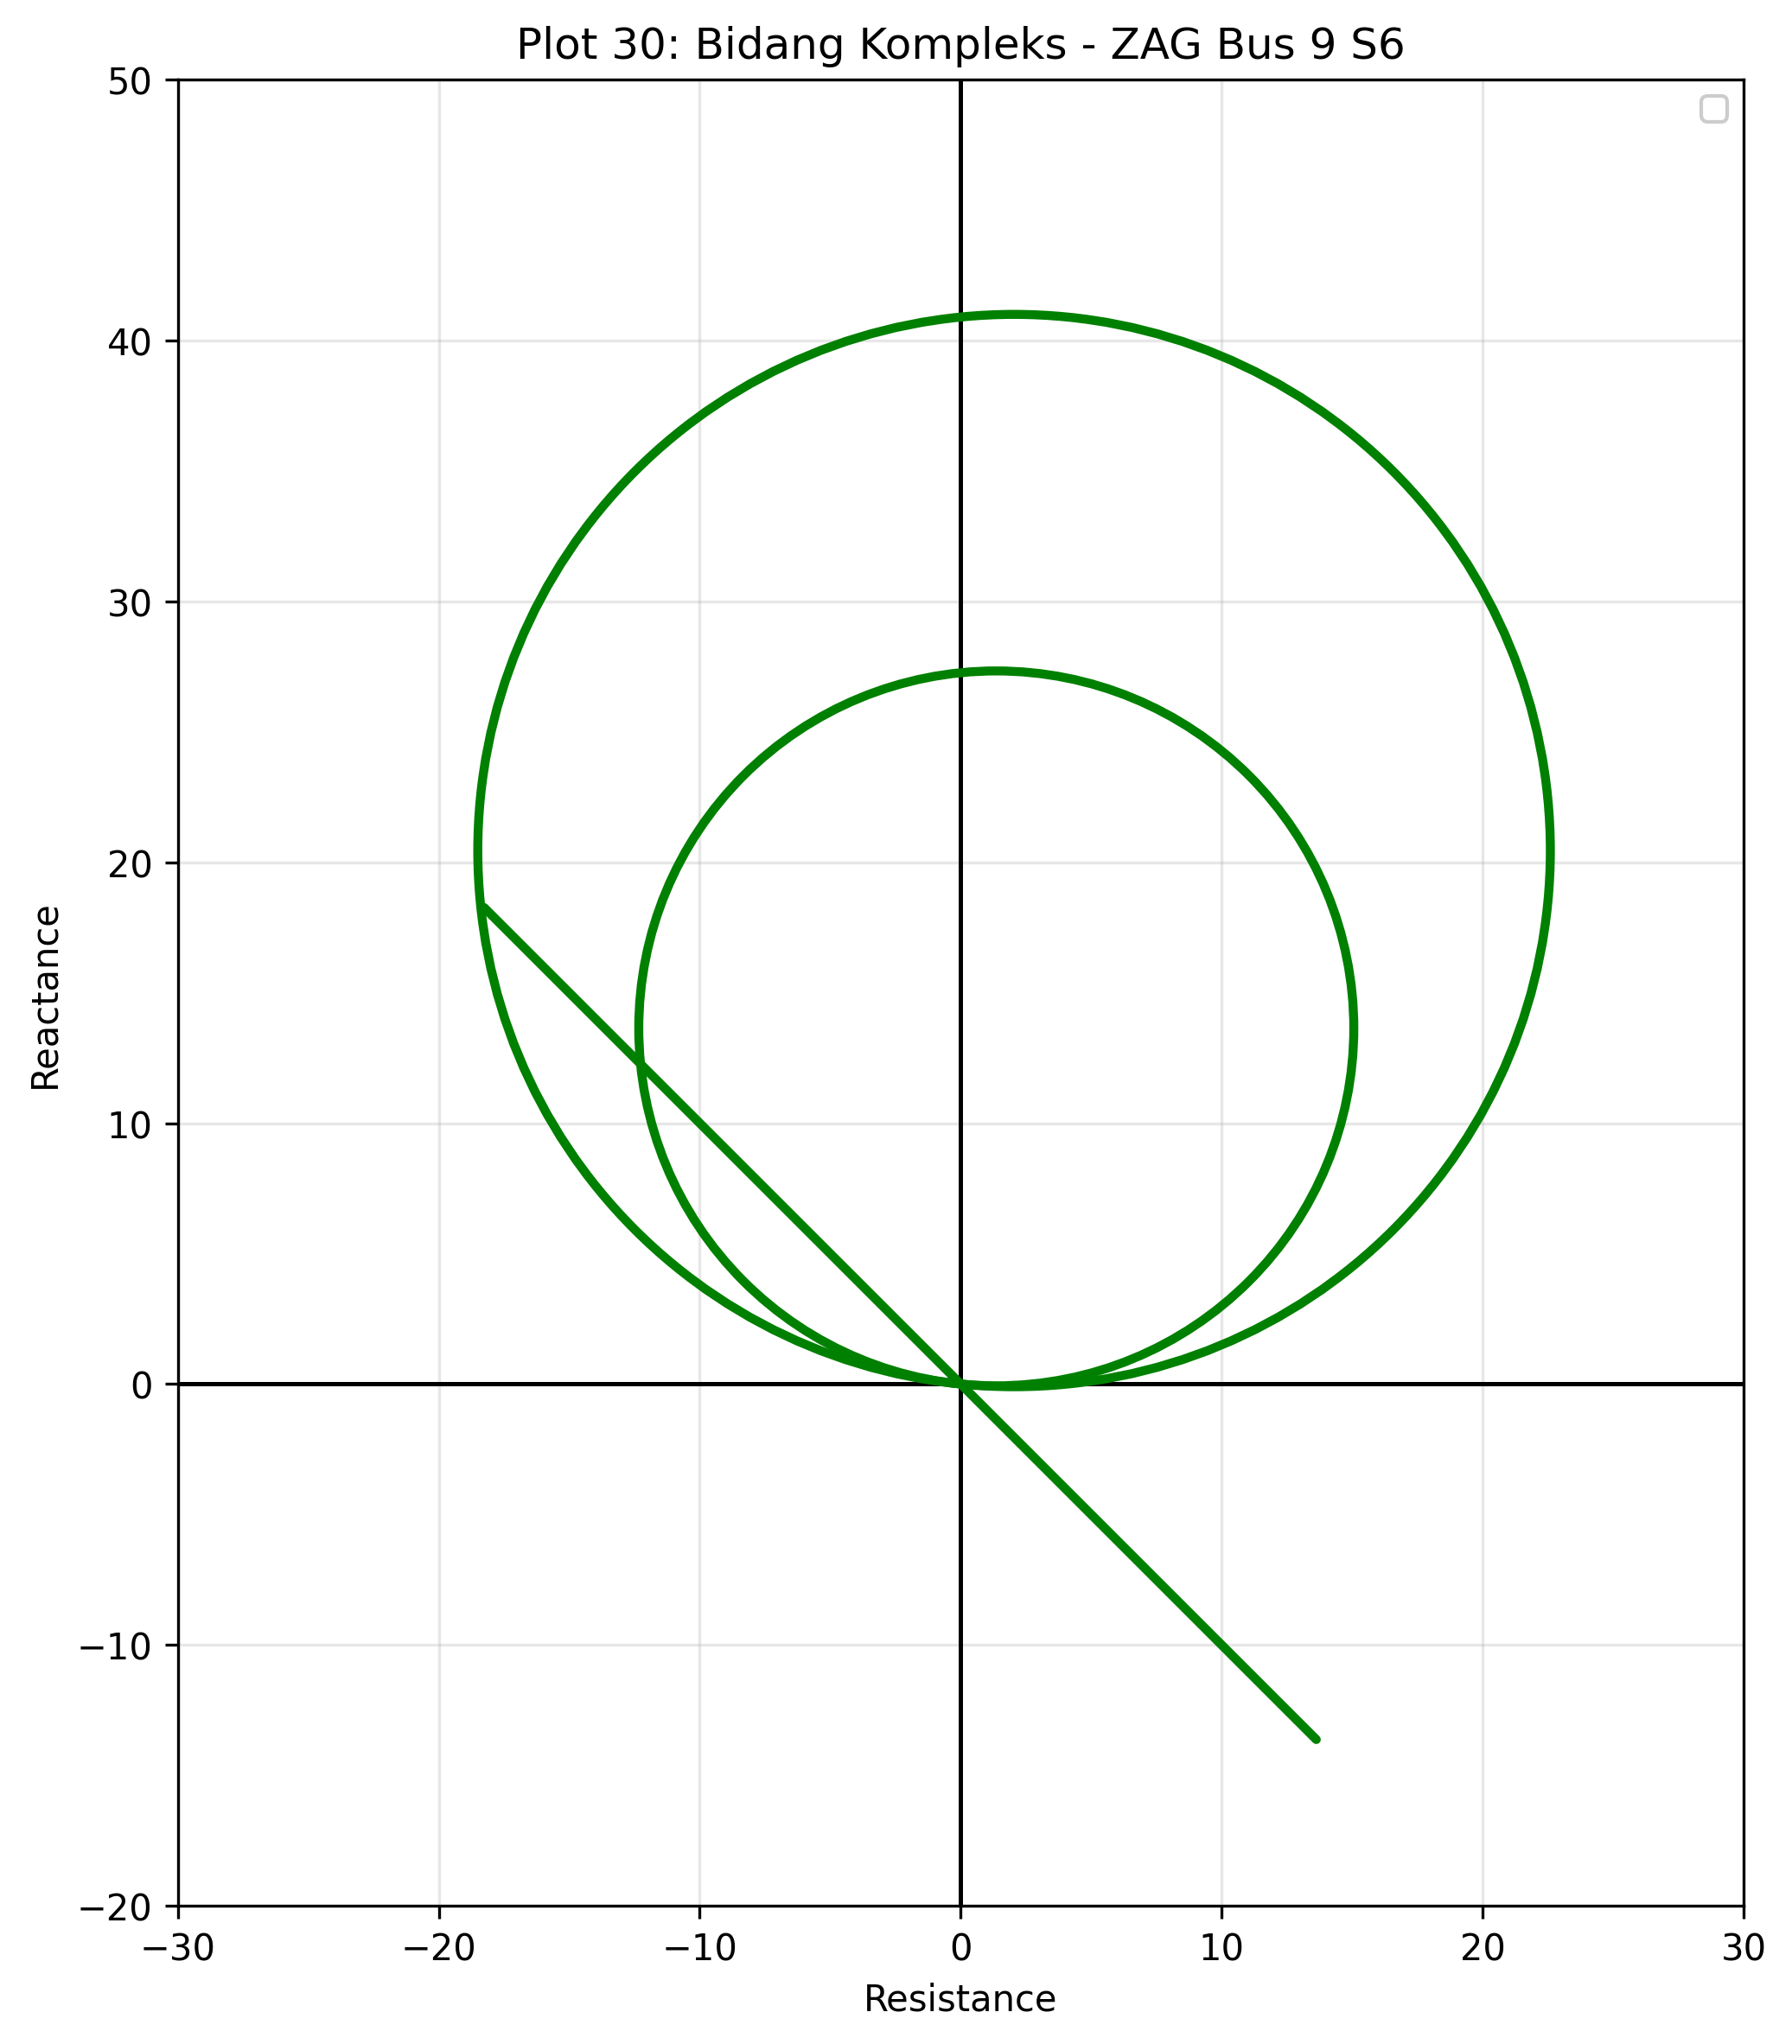
\includegraphics[width=\textwidth]{contents/chapter-4/PRIZI_30_ZAG_Bus_9_S6.png}
        \caption{Zoom In Pada Zona Proteksi}
        \label{fig:PRIZI_30_ZAG_Bus_9_S6}
    \end{subfigure}

    \caption{Impedansi Tampak ZAG Bus 9 Skenario 6}
    \label{fig:Impedansi_Tampak_ZAG_Bus_9_S6}
\end{figure}

Terlihat pada gambar \ref{fig:Impedansi_Tampak_ZAG_Bus_9_S6} bahwa impedansi tampak pada fasa B dengan ground yang dibaca oleh relay 21 sisi bus 9 saat terdapat gangguan bekerja dengan baik sesuai acuan pada \ref{subsec:tanpa_IBR_ex_dlg} relay 21 bus 9 tidak mendeteksi adanya gangguan sehingga tidak mengirimkan sinyal trip kepada CB.



%%%%%%%%%%%%%%%%%%%%%%%%%%%%%%%%%%%%%%%%%%%%%%%%%%%%%%%%%%%%%%

% \begin{figure}[H]
%     \centering
%     \includegraphics[width=0.8\textwidth]{contents/chapter-4/31_ZBG_Bus_9_S6_dengan_lingkaran_dan_garis.png}
%     \caption{Impedansi Tampak ZBG Bus 9 Skenario 6}
%     \label{fig:31_ZBG_Bus_9_S6_dengan_lingkaran_dan_garis}
% \end{figure}

%%%%%%%%%%%%%%%%%%%%%%%%%%%%%%%%%SISI PRIMER%%%%%%%%%%%%%%%%%%%%%%%%%%%%%%%%%%

% \begin{figure}[H]
%     \centering
%     \includegraphics[width=0.8\textwidth]{contents/chapter-4/PRIA_31_ZBG_Bus_9_S6.png}
%     \caption{Impedansi Tampak ZBG Bus 9 Skenario 6}
%     \label{fig:PRIA_31_ZBG_Bus_9_S6}
% \end{figure}

% \begin{figure}[H]
%     \centering
%     \includegraphics[width=0.8\textwidth]{contents/chapter-4/PRIZI_31_ZBG_Bus_9_S6.png}
%     \caption{Impedansi Tampak ZBG Bus 9 Skenario 6}
%     \label{fig:PRIZI_31_ZBG_Bus_9_S6}
% \end{figure}

\begin{figure}[H]
    \centering

    % Gambar sebelah kiri
    \begin{subfigure}[t]{0.48\textwidth}
        \centering
        \includegraphics[width=\textwidth]{contents/chapter-4/PRIA_31_ZBG_Bus_9_S6.png}
        \caption{Seluruh Impedansi Tampak}
        \label{fig:PRIA_31_ZBG_Bus_9_S6}
    \end{subfigure}
    \hfill
    % Gambar sebelah kanan
    \begin{subfigure}[t]{0.48\textwidth}
        \centering
        \includegraphics[width=\textwidth]{contents/chapter-4/PRIZI_31_ZBG_Bus_9_S6.png}
        \caption{Zoom In Pada Zona Proteksi}
        \label{fig:PRIZI_31_ZBG_Bus_9_S6}
    \end{subfigure}

    \caption{Impedansi Tampak ZBG Bus 9 Skenario 6}
    \label{fig:Impedansi_Tampak_ZBG_Bus_9_S6}
\end{figure}

Terlihat pada gambar \ref{fig:Impedansi_Tampak_ZBG_Bus_9_S6} bahwa impedansi tampak pada fasa B dengan ground yang dibaca oleh relay 21 sisi bus 9 saat terdapat gangguan bekerja dengan baik sesuai acuan pada \ref{subsec:tanpa_IBR_ex_dlg} relay 21 bus 9 tidak mendeteksi adanya gangguan sehingga tidak mengirimkan sinyal trip kepada CB. Walaupun impedansi tampak yang terlihat memasuki zona 1 namun elemen phase directional tidak membaca gangguan terdapat di arah depan relay. 



%%%%%%%%%%%%%%%%%%%%%%%%%%%%%%%%%%%%%%%%%%%%%%%%%%%%%%%%%%%%%%

% \begin{figure}[H]
%     \centering
%     \includegraphics[width=0.8\textwidth]{contents/chapter-4/32_ZAB_Bus_9_S6_dengan_lingkaran_dan_garis.png}
%     \caption{Impedansi Tampak ZAB Bus 9 Skenario 6}
%     \label{fig:32_ZAB_Bus_9_S6_dengan_lingkaran_dan_garis}
% \end{figure}

% pada gambar \ref{fig:27_ZAG_Bus_8_S6_dengan_lingkaran_dan_garis} hingga \ref{fig:29_ZAB_Bus_8_S6_dengan_lingkaran_dan_garis} merupakan impendansi tampak yang di baca oleh relay 21 dari sisi bus 8 yang menunjukkan bahwa relay mengalami misoperation dikarenakan nilaii impedansi yang menjadi sangat besar dan semakin menjauh dari zona yang ditentukan. Kemudian pada gambar \ref{fig:30_ZAG_Bus_9_S6_dengan_lingkaran_dan_garis} hingga \ref{fig:32_ZAB_Bus_9_S6_dengan_lingkaran_dan_garis} merupakan impendansi tampak yang dibaca oleh relay 21 dari sisi bus 9 yang menunjukkan terdapat misoperation karena melewati batas untuk zona 1.

%%%%%%%%%%%%%%%%%%%%%%%%%%%%%%%%%SISI PRIMER%%%%%%%%%%%%%%%%%%%%%%%%%%%%%%%%%%

% \begin{figure}[H]
%     \centering
%     \includegraphics[width=0.8\textwidth]{contents/chapter-4/PRIA_32_ZAB_Bus_9_S6.png}
%     \caption{Impedansi Tampak ZAB Bus 9 Skenario 6}
%     \label{fig:PRIA_32_ZAB_Bus_9_S6}
% \end{figure}

% \begin{figure}[H]
%     \centering
%     \includegraphics[width=0.8\textwidth]{contents/chapter-4/PRIZI_32_ZAB_Bus_9_S6.png}
%     \caption{Impedansi Tampak ZAB Bus 9 Skenario 6}
%     \label{fig:PRIZI_32_ZAB_Bus_9_S6}
% \end{figure}

\begin{figure}[H]
    \centering

    % Gambar sebelah kiri
    \begin{subfigure}[t]{0.48\textwidth}
        \centering
        \includegraphics[width=\textwidth]{contents/chapter-4/PRIA_32_ZAB_Bus_9_S6.png}
        \caption{Seluruh Impedansi Tampak}
        \label{fig:PRIA_32_ZAB_Bus_9_S6}
    \end{subfigure}
    \hfill
    % Gambar sebelah kanan
    \begin{subfigure}[t]{0.48\textwidth}
        \centering
        \includegraphics[width=\textwidth]{contents/chapter-4/PRIZI_32_ZAB_Bus_9_S6.png}
        \caption{Zoom In Pada Zona Proteksi}
        \label{fig:PRIZI_32_ZAB_Bus_9_S6}
    \end{subfigure}

    \caption{Impedansi Tampak ZAB Bus 9 Skenario 6}
    \label{fig:Impedansi_Tampak_ZAB_Bus_9_S6}
\end{figure}

Terlihat pada gambar \ref{fig:Impedansi_Tampak_ZAB_Bus_9_S6} bahwa impedansi tampak pada fasa A dengan fasa B yang dibaca oleh relay 21 sisi bus 9 saat terdapat gangguan bekerja dengan baik sesuai acuan pada \ref{subsec:tanpa_IBR_ex_dlg} relay 21 bus 9 tidak mendeteksi adanya gangguan sehingga tidak mengirimkan sinyal trip kepada CB.



%%%%%%%%%%%%%%%%%%%%%%%%%%%%%%%%%%%%%%%%%%%%%%%%%%%%%%%%%%%%%%

\section{Perbandingan Karakteristik Relay 21 antar Jenis IBR}

Hasil pada bagian sebelumnya menunjukkan bahwa respons relay 21 sangat dipengaruhi oleh kombinasi lokasi gangguan, konfigurasi jaringan, dan kontribusi arus dari sisi sumber. Pada skenario 1 dengan \textit{wind turbine type 3} dan gangguan internal DLG pada TL89, relay 21 pada sisi Bus 8 dan Bus 9 masih bekerja sesuai acuan kondisi dasar. Impedansi tampak yang terbaca tetap berada pada daerah operasi yang sesuai, sehingga integrasi IBR pada skenario tersebut tidak menimbulkan penyimpangan keputusan trip.

Pola yang berbeda muncul pada gangguan eksternal di TL79 dengan kondisi TL78 \textit{out of service}. Pada skenario 3, 4, dan 5 dengan \textit{wind turbine type 3}, impedansi tampak pada sisi Bus 8 tidak masuk ke zona proteksi dan arus gangguan yang terbaca tidak memenuhi syarat \textit{starting}. Pola yang sama juga terlihat pada skenario 2 dengan \textit{wind turbine type 4} dan skenario 6 dengan \textit{photovoltaic}. Dengan demikian, kondisi paling kritis untuk relay 21 pada hasil ini bukan hanya ditentukan oleh jenis IBR, tetapi oleh gangguan eksternal pada TL79 ketika konfigurasi jaringan membuat kontribusi arus pada sisi Bus 8 menjadi rendah.

Jika dibandingkan antarjenis IBR, data yang ditampilkan menunjukkan bahwa \textit{wind turbine type 4} dan \textit{photovoltaic} menghasilkan pola penyimpangan yang serupa dengan skenario eksternal pada \textit{wind turbine type 3}. Sisi Bus 8 menjadi sisi yang paling terdampak karena impedansi tampak tidak masuk ke zona dan syarat arus awal operasi tidak terpenuhi. Sementara itu, sisi Bus 9 umumnya tetap tidak trip karena gangguan tidak terbaca sebagai gangguan di arah depan relay. Pada skenario PV, terdapat elemen yang sempat masuk zona 1, tetapi elemen \textit{directional} tetap menahan operasi karena arah gangguan tidak terbaca sebagai arah depan.

Secara umum, relay 21 masih dapat bekerja sesuai acuan untuk gangguan internal pada saluran yang diproteksi. Namun, pada gangguan eksternal dengan konfigurasi jaringan tertentu, integrasi IBR menyebabkan perubahan besaran yang dibaca relay sehingga keputusan operasi pada sisi Bus 8 tidak lagi mengikuti acuan kondisi dasar.

\begin{table}[H]
    \centering
    \caption{Ringkasan Respons Relay 21 pada Sistem dengan Integrasi IBR}
    \label{tab:ringkasan_respons_relay21_ibr}
    \resizebox{\textwidth}{!}{%
        \begin{tabular}{|c|c|c|p{2.7cm}|p{4.2cm}|p{3.0cm}|p{5.4cm}|}
            \hline
            \textbf{Jenis IBR} & \textbf{Skenario} & \textbf{Gangguan} & \textbf{Sisi Relay} & \textbf{Respons Utama} & \textbf{Status Operasi} & \textbf{Alasan} \\ \hline
            Wind Turbine Type 3 & 1 & Internal DLG pada TL89 & Bus 8 dan Bus 9 & Kontribusi IBR tidak mendominasi sehingga respons relay masih mengikuti karakteristik kondisi dasar. & Sesuai acuan & Kontribusi dari sisi IBR tidak mendominasi karena TL78 tetap aktif, sehingga kinerja proteksi masih didominasi oleh sistem tenaga konvensional dan relay bekerja sesuai acuan kondisi dasar. \\ \hline
            Wind Turbine Type 3 & 3 & External DLG pada TL79 & Bus 8 dan Bus 9 & Sisi Bus 8 tidak memenuhi syarat \textit{starting}, sedangkan sisi Bus 9 tidak mengirimkan sinyal trip. & Bus 8 mengalami \textit{misoperation}; Bus 9 sesuai acuan & Pada sisi Bus 8, arus yang terbaca tidak memenuhi arus minimum untuk relay aktif. Pada sisi Bus 9, relay tidak mendeteksi gangguan eksternal sebagai gangguan yang perlu dioperasikan. \\ \hline
            Wind Turbine Type 3 & 4 & External 3P pada TL79 & Bus 8 dan Bus 9 & Sisi Bus 8 tidak memenuhi syarat \textit{starting}, sedangkan sisi Bus 9 tidak mengirimkan sinyal trip. & Bus 8 mengalami \textit{misoperation}; Bus 9 sesuai acuan & Pada sisi Bus 8, arus gangguan cukup kecil dan tidak membuat relay aktif karena tidak memenuhi syarat \textit{starting}. Pada sisi Bus 9, relay tidak mendeteksi gangguan sehingga tidak mengirimkan sinyal trip. \\ \hline
            Wind Turbine Type 3 & 5 & External SLG pada TL79 & Bus 8 dan Bus 9 & Sisi Bus 8 tidak memenuhi syarat \textit{starting}, sedangkan sisi Bus 9 tidak mengirimkan sinyal trip. & Bus 8 mengalami \textit{misoperation}; Bus 9 sesuai acuan & Pada sisi Bus 8, arus gangguan cukup kecil dan tidak membuat relay aktif karena tidak memenuhi syarat \textit{starting}. Pada sisi Bus 9, relay bekerja sesuai acuan karena tidak mendeteksi gangguan dan tidak mengirimkan sinyal trip. \\ \hline
            Wind Turbine Type 4 & 2 & External DLG pada TL79 & Bus 8 dan Bus 9 & Sisi Bus 8 tidak memenuhi syarat \textit{starting}, sedangkan sisi Bus 9 tidak mengirimkan sinyal trip. & Bus 8 mengalami \textit{misoperation}; Bus 9 sesuai acuan & Pada sisi Bus 8, arus gangguan cukup kecil dan tidak membuat relay aktif karena tidak memenuhi syarat \textit{starting}. Pada sisi Bus 9, relay tidak mendeteksi adanya gangguan sehingga tidak mengirimkan sinyal trip. \\ \hline
            Photovoltaic & 6 & External DLG pada TL79 & Bus 8 dan Bus 9 & Sisi Bus 8 tidak memenuhi syarat \textit{starting}; pada sisi Bus 9, elemen \textit{directional} menahan operasi relay. & Bus 8 mengalami \textit{misoperation}; Bus 9 sesuai acuan & Pada sisi Bus 8, arus gangguan cukup kecil dan tidak membuat relay aktif karena tidak memenuhi syarat \textit{starting}. Pada sisi Bus 9, elemen \textit{directional} tidak membaca gangguan berada di arah depan relay. \\ \hline
        \end{tabular}%
    }
\end{table}

\section{Implikasi Penggunaan Setting Konvensional pada Relay 21}

Penggunaan setting konvensional pada relay 21 masih layak untuk kondisi yang karakteristik gangguannya mendekati kondisi dasar. Hal ini terlihat pada gangguan internal DLG skenario 1, ketika relay 21 pada kedua sisi saluran masih mendeteksi gangguan dan memberikan keputusan trip sesuai acuan. Pada kondisi tersebut, integrasi \textit{wind turbine type 3} tidak mengubah pembacaan impedansi tampak secara signifikan terhadap keputusan operasi relay.

Penyimpangan mulai muncul pada gangguan eksternal di sekitar TL89 ketika konfigurasi jaringan berubah dan kontribusi arus pada sisi relay menjadi rendah. Pada skenario 2, 3, 4, 5, dan 6, sisi Bus 8 menunjukkan kecenderungan impedansi tampak berada di luar zona proteksi disertai arus gangguan yang tidak memenuhi syarat \textit{starting}. Temuan ini menunjukkan bahwa setting konvensional tidak selalu cukup untuk menjaga respons relay 21 ketika sumber arus gangguan didominasi atau dipengaruhi oleh karakteristik IBR.

Berdasarkan hasil tersebut, setting konvensional relay 21 tidak dapat langsung dianggap memadai untuk seluruh skenario sistem dengan IBR. Evaluasi ulang diperlukan terutama untuk kondisi gangguan eksternal, konfigurasi saluran \textit{out of service}, dan kondisi ketika arus gangguan yang terbaca oleh relay menjadi lebih kecil dari asumsi sistem konvensional. Temuan ini menjadi dasar untuk pembahasan kebutuhan penyesuaian setting atau strategi proteksi tambahan pada bagian kesimpulan dan saran.

\section{Respons Relay 87L pada Sistem dengan WT Type 3}

Bagian ini membahas respons relay 87L pada sistem dengan \textit{wind turbine type 3}. Berbeda dari relay 21 yang dianalisis melalui impedansi tampak, relay 87L dianalisis berdasarkan posisi titik arus diferensial terhadap arus \textit{restraint}. Titik yang berada di atas batas operasi menunjukkan kondisi trip, sedangkan titik yang berada di bawah batas operasi menunjukkan relay tetap tertahan.

Skenario yang dibahas mencakup gangguan internal DLG pada TL89 serta gangguan eksternal DLG, tiga fasa, dan SLG pada TL79. Dengan susunan ini, respons relay 87L dapat dibandingkan antara gangguan pada daerah proteksi dan gangguan di luar daerah proteksi.

\subsection{Skenario 1 : Wind Turbine Type 3 Internal DLG Fault}

\begin{figure}[H]
    \centering
    \includegraphics[width=0.8\textwidth]{contents/chapter-4/plot_Ax1_Ay1.png}
    \caption{Current Comparison Differential Fasa A Skenario 1}
    \label{fig:plot_Ax1_Ay1}
\end{figure}

Terlihat pada gambar \ref{fig:plot_Ax1_Ay1} arus diferensial dan arus penahan fasa A saat adanya gangguan internal DLG menunjukkan bahwa arus berada di atas batas yang ditentukan oleh setting relay. Relay mendeteksi adanya gangguan kemudian memerintahkan CB untuk trip. Relay 87L beroperasi dengan benar berdasarkan acuan pada \ref{subsec:tanpa_IBR_in_dlg}.

\begin{figure}[H]
    \centering
    \includegraphics[width=0.8\textwidth]{contents/chapter-4/plot_Bx1_By1.png}
    \caption{Current Comparison Differential Fasa B Skenario 1}
    \label{fig:plot_Bx1_By1}
\end{figure}

Terlihat pada gambar \ref{fig:plot_Bx1_By1} arus diferensial dan arus penahan fasa B saat adanya gangguan internal DLG menunjukkan bahwa arus berada di atas batas yang ditentukan oleh setting relay. Relay mendeteksi adanya gangguan kemudian memerintahkan CB untuk trip. Relay 87L beroperasi dengan benar berdasarkan acuan pada \ref{subsec:tanpa_IBR_in_dlg}.

\begin{figure}[H]
    \centering
    \includegraphics[width=0.8\textwidth]{contents/chapter-4/plot_Cx1_Cy1.png}
    \caption{Current Comparison Differential Fasa C Skenario 1}
    \label{fig:plot_Cx1_Cy1}
\end{figure}

Terlihat pada gambar \ref{fig:plot_Cx1_Cy1} arus diferensial dan arus penahan fasa C saat adanya gangguan internal DLG menunjukkan bahwa arus berada di atas batas yang ditentukan oleh setting relay. Relay mendeteksi adanya gangguan kemudian memerintahkan CB untuk trip. Relay 87L beroperasi dengan benar berdasarkan acuan pada \ref{subsec:tanpa_IBR_in_dlg}.


\subsection{Skenario 3 : Wind Turbine Type 3 External DLG Fault}

\begin{figure}[H]
    \centering
    \includegraphics[width=0.8\textwidth]{contents/chapter-4/plot_Ax3_Ay3.png}
    \caption{Current Comparison Differential Fasa A Skenario 3}
    \label{fig:plot_Ax3_Ay3}
\end{figure}

Terlihat pada gambar \ref{fig:plot_Ax3_Ay3} arus diferensial dan arus penahan fasa A saat adanya gangguan external DLG menunjukkan bahwa arus berada di bawah batas yang ditentukan oleh setting relay. Relay tidak mendeteksi adanya gangguan maka relay tidak memerintahkan CB untuk trip. Relay 87L beroperasi dengan benar berdasarkan acuan pada \ref{subsec:tanpa_IBR_ex_dlg}.

\begin{figure}[H]
    \centering
    \includegraphics[width=0.8\textwidth]{contents/chapter-4/plot_Bx3_By3.png}
    \caption{Current Comparison Differential Fasa B Skenario 3}
    \label{fig:plot_Bx3_By3}
\end{figure}

Terlihat pada gambar \ref{fig:plot_Bx3_By3} arus diferensial dan arus penahan fasa B saat adanya gangguan external DLG menunjukkan bahwa arus berada di bawah batas yang ditentukan oleh setting relay. Relay tidak mendeteksi adanya gangguan maka relay tidak memerintahkan CB untuk trip. Relay 87L beroperasi dengan benar berdasarkan acuan pada \ref{subsec:tanpa_IBR_ex_dlg}.

\begin{figure}[H]
    \centering
    \includegraphics[width=0.8\textwidth]{contents/chapter-4/plot_Cx3_Cy3.png}
    \caption{Current Comparison Differential Fasa C Skenario 3}
    \label{fig:plot_Cx3_Cy3}
\end{figure}

Terlihat pada gambar \ref{fig:plot_Cx3_Cy3} arus diferensial dan arus penahan fasa C saat adanya gangguan external DLG menunjukkan bahwa arus berada di bawah batas yang ditentukan oleh setting relay. Relay tidak mendeteksi adanya gangguan maka relay tidak memerintahkan CB untuk trip. Relay 87L beroperasi dengan benar berdasarkan acuan pada \ref{subsec:tanpa_IBR_ex_dlg}.

\subsection{Skenario 4 : Wind Turbine Type 3 External 3P Fault}

\begin{figure}[H]
    \centering
    \includegraphics[width=0.8\textwidth]{contents/chapter-4/plot_Ax4_Ay4.png}
    \caption{Current Comparison Differential Fasa A Skenario 4}
    \label{fig:plot_Ax4_Ay4}
\end{figure}

Terlihat pada gambar \ref{fig:plot_Ax4_Ay4} arus diferensial dan arus penahan fasa A saat adanya gangguan external 3P menunjukkan bahwa arus berada di bawah batas yang ditentukan oleh setting relay. Relay tidak mendeteksi adanya gangguan maka relay tidak memerintahkan CB untuk trip. Relay 87L beroperasi dengan benar berdasarkan acuan pada \ref{subsec:tanpa_IBR_ex_3p}.


\begin{figure}[H]
    \centering
    \includegraphics[width=0.8\textwidth]{contents/chapter-4/plot_Bx4_By4.png}
    \caption{Current Comparison Differential Fasa B Skenario 4}
    \label{fig:plot_Bx4_By4}
\end{figure}

Terlihat pada gambar \ref{fig:plot_Bx4_By4} arus diferensial dan arus penahan fasa B saat adanya gangguan external 3P menunjukkan bahwa arus berada di bawah batas yang ditentukan oleh setting relay. Relay tidak mendeteksi adanya gangguan maka relay tidak memerintahkan CB untuk trip. Relay 87L beroperasi dengan benar berdasarkan acuan pada \ref{subsec:tanpa_IBR_ex_3p}.

\begin{figure}[H]
    \centering
    \includegraphics[width=0.8\textwidth]{contents/chapter-4/plot_Cx4_Cy4.png}
    \caption{Current Comparison Differential Fasa C Skenario 4}
    \label{fig:plot_Cx4_Cy4}
\end{figure}

Terlihat pada gambar \ref{fig:plot_Cx4_Cy4} arus diferensial dan arus penahan fasa C saat adanya gangguan external 3P menunjukkan bahwa arus berada di bawah batas yang ditentukan oleh setting relay. Relay tidak mendeteksi adanya gangguan maka relay tidak memerintahkan CB untuk trip. Relay 87L beroperasi dengan benar berdasarkan acuan pada \ref{subsec:tanpa_IBR_ex_3p}.

\subsection{Skenario 5 : Wind Turbine Type 3 External SLG Fault}

\begin{figure}[H]
    \centering
    \includegraphics[width=0.8\textwidth]{contents/chapter-4/plot_Ax5_Ay5.png}
    \caption{Current Comparison Differential Fasa A Skenario 5}
    \label{fig:plot_Ax5_Ay5}
\end{figure}

Terlihat pada gambar \ref{fig:plot_Ax5_Ay5} arus diferensial dan arus penahan fasa A saat adanya gangguan external SLG menunjukkan bahwa arus berada di bawah batas yang ditentukan oleh setting relay. Relay tidak mendeteksi adanya gangguan maka relay tidak memerintahkan CB untuk trip. Relay 87L beroperasi dengan benar berdasarkan acuan pada \ref{subsec:tanpa_IBR_ex_slg}.

\begin{figure}[H]
    \centering
    \includegraphics[width=0.8\textwidth]{contents/chapter-4/plot_Bx5_By5.png}
    \caption{Current Comparison Differential Fasa B Skenario 5}
    \label{fig:plot_Bx5_By5}
\end{figure}

Terlihat pada gambar \ref{fig:plot_Bx5_By5} arus diferensial dan arus penahan fasa B saat adanya gangguan external SLG menunjukkan bahwa arus berada di bawah batas yang ditentukan oleh setting relay. Relay tidak mendeteksi adanya gangguan maka relay tidak memerintahkan CB untuk trip. Relay 87L beroperasi dengan benar berdasarkan acuan pada \ref{subsec:tanpa_IBR_ex_slg}.


\begin{figure}[H]
    \centering
    \includegraphics[width=0.8\textwidth]{contents/chapter-4/plot_Cx5_Cy5.png}
    \caption{Current Comparison Differential Fasa C Skenario 5}
    \label{fig:plot_Cx5_Cy5}
\end{figure}

Terlihat pada gambar \ref{fig:plot_Cx5_Cy5} arus diferensial dan arus penahan fasa C saat adanya gangguan external SLG menunjukkan bahwa arus berada di bawah batas yang ditentukan oleh setting relay. Relay tidak mendeteksi adanya gangguan maka relay tidak memerintahkan CB untuk trip. Relay 87L beroperasi dengan benar berdasarkan acuan pada \ref{subsec:tanpa_IBR_ex_slg}.

\section{Respons Relay 87L pada Sistem dengan WT Type 4}

Bagian ini membahas respons relay 87L ketika sistem menggunakan \textit{wind turbine type 4}. Struktur pembahasan dibuat sama dengan bagian sebelumnya, yaitu dengan melihat posisi titik arus diferensial terhadap arus \textit{restraint}. Skenario yang diamati adalah gangguan eksternal DLG pada TL79 dengan TL78 \textit{out of service}.

\subsection{Skenario 2 : Wind Turbine Type 4 External DLG Fault}

\begin{figure}[H]
    \centering
    \includegraphics[width=0.8\textwidth]{contents/chapter-4/plot_Ax2_Ay2.png}
    \caption{Current Comparison Differential Fasa A Skenario 2}
    \label{fig:plot_Ax2_Ay2}
\end{figure}

Terlihat pada gambar \ref{fig:plot_Ax2_Ay2} arus diferensial dan arus penahan fasa A saat adanya gangguan external DLG menunjukkan bahwa arus berada di bawah batas yang ditentukan oleh setting relay. Relay tidak mendeteksi adanya gangguan maka relay tidak memerintahkan CB untuk trip. Relay 87L beroperasi dengan benar berdasarkan acuan pada \ref{subsec:tanpa_IBR_ex_dlg}.

\begin{figure}[H]
    \centering
    \includegraphics[width=0.8\textwidth]{contents/chapter-4/plot_Bx2_By2.png}
    \caption{Current Comparison Differential Fasa B Skenario 2}
    \label{fig:plot_Bx2_By2}
\end{figure}

Terlihat pada gambar \ref{fig:plot_Bx2_By2} arus diferensial dan arus penahan fasa B saat adanya gangguan external DLG menunjukkan bahwa arus berada di bawah batas yang ditentukan oleh setting relay. Relay tidak mendeteksi adanya gangguan maka relay tidak memerintahkan CB untuk trip. Relay 87L beroperasi dengan benar berdasarkan acuan pada \ref{subsec:tanpa_IBR_ex_dlg}.

\begin{figure}[H]
    \centering
    \includegraphics[width=0.8\textwidth]{contents/chapter-4/plot_Cx2_Cy2.png}
    \caption{Current Comparison Differential Fasa C Skenario 2}
    \label{fig:plot_Cx2_Cy2}
\end{figure}

Terlihat pada gambar \ref{fig:plot_Cx2_Cy2} arus diferensial dan arus penahan fasa C saat adanya gangguan external DLG menunjukkan bahwa arus berada di bawah batas yang ditentukan oleh setting relay. Relay tidak mendeteksi adanya gangguan maka relay tidak memerintahkan CB untuk trip. Relay 87L beroperasi dengan benar berdasarkan acuan pada \ref{subsec:tanpa_IBR_ex_dlg}.

\section{Respons Relay 87L pada Sistem dengan Photovoltaic}

Bagian ini membahas respons relay 87L ketika sistem menggunakan \textit{photovoltaic}. Skenario yang diamati adalah gangguan eksternal DLG pada TL79 dengan TL78 \textit{out of service}. Analisis difokuskan pada apakah titik arus diferensial dan arus \textit{restraint} masih berada di daerah penahan atau bergeser ke daerah operasi.

\subsection{Skenario 6 : Photovoltaic External DLG Fault}

\begin{figure}[H]
    \centering
    \includegraphics[width=0.8\textwidth]{contents/chapter-4/plot_Ax6_Ay6.png}
    \caption{Current Comparison Differential Fasa A Skenario 6}
    \label{fig:plot_Ax6_Ay6}
\end{figure}

Terlihat pada gambar \ref{fig:plot_Ax6_Ay6} arus diferensial dan arus penahan fasa A saat adanya gangguan external DLG menunjukkan bahwa arus berada di bawah batas yang ditentukan oleh setting relay. Relay tidak mendeteksi adanya gangguan maka relay tidak memerintahkan CB untuk trip. Relay 87L beroperasi dengan benar berdasarkan acuan pada \ref{subsec:tanpa_IBR_ex_dlg}.

\begin{figure}[H]
    \centering
    \includegraphics[width=0.8\textwidth]{contents/chapter-4/plot_Bx6_By6.png}
    \caption{Current Comparison Differential Fasa B Skenario 6}
    \label{fig:plot_Bx6_By6}
\end{figure}

Terlihat pada gambar \ref{fig:plot_Bx6_By6} arus diferensial dan arus penahan fasa B saat adanya gangguan external DLG menunjukkan bahwa arus berada di bawah batas yang ditentukan oleh setting relay. Relay tidak mendeteksi adanya gangguan maka relay tidak memerintahkan CB untuk trip. Relay 87L beroperasi dengan benar berdasarkan acuan pada \ref{subsec:tanpa_IBR_ex_dlg}.

\begin{figure}[H]
    \centering
    \includegraphics[width=0.8\textwidth]{contents/chapter-4/plot_Cx6_Cy6.png}
    \caption{Current Comparison Differential Fasa C Skenario 6}
    \label{fig:plot_Cx6_Cy6}
\end{figure}

Terlihat pada gambar \ref{fig:plot_Cx6_Cy6} arus diferensial dan arus penahan fasa C saat adanya gangguan external DLG menunjukkan bahwa arus berada di bawah batas yang ditentukan oleh setting relay. Relay tidak mendeteksi adanya gangguan maka relay tidak memerintahkan CB untuk trip. Relay 87L beroperasi dengan benar berdasarkan acuan pada \ref{subsec:tanpa_IBR_ex_dlg}.

\section{Perbandingan Karakteristik Relay 87L antar Jenis IBR}

Berdasarkan hasil yang ditampilkan, relay 87L menunjukkan respons yang lebih konsisten dibandingkan relay 21 pada skenario yang diuji. Pada skenario internal DLG dengan \textit{wind turbine type 3}, titik arus diferensial berada di atas batas operasi sehingga relay memerintahkan trip. Sebaliknya, pada gangguan eksternal DLG, tiga fasa, dan SLG, titik arus berada di bawah batas operasi sehingga relay tetap tidak trip.

Pada \textit{wind turbine type 4} dan \textit{photovoltaic}, skenario yang ditampilkan adalah gangguan eksternal DLG. Untuk kedua jenis IBR tersebut, titik arus pada fasa A, B, dan C tetap berada di bawah batas operasi relay. Dengan demikian, tidak terlihat perubahan keputusan operasi relay 87L akibat pergantian jenis IBR pada skenario eksternal DLG yang diuji.

Pola umum yang dapat ditarik adalah bahwa relay 87L masih mampu membedakan gangguan internal dan eksternal berdasarkan hubungan arus diferensial dan arus \textit{restraint}. Pada hasil yang tersedia di Bab ini, belum terdapat indikasi relay 87L mengalami salah trip untuk gangguan eksternal maupun gagal trip untuk gangguan internal. Namun, kesimpulan ini hanya berlaku untuk skenario dan setting yang diuji pada penelitian ini.

\begin{table}[H]
    \centering
    \caption{Ringkasan Respons Relay 87L pada Sistem dengan Integrasi IBR}
    \label{tab:ringkasan_respons_relay87l_ibr}
    \resizebox{\textwidth}{!}{%
        \begin{tabular}{|c|c|c|c|p{4.2cm}|p{2.8cm}|p{5.4cm}|}
            \hline
            \textbf{Jenis IBR} & \textbf{Skenario} & \textbf{Gangguan} & \textbf{Fasa} & \textbf{Respons terhadap Batas Operasi} & \textbf{Status Operasi} & \textbf{Alasan} \\ \hline
            Wind Turbine Type 3 & 1 & Internal DLG pada TL89 & A, B, C & Arus diferensial berada di atas batas operasi relay. & Trip, sesuai acuan & Arus diferensial dan arus penahan berada di atas batas yang ditentukan oleh setting relay, sehingga relay mendeteksi gangguan internal dan memerintahkan CB untuk trip. \\ \hline
            Wind Turbine Type 3 & 3 & External DLG pada TL79 & A, B, C & Arus diferensial berada di bawah batas operasi relay. & Tidak trip, sesuai acuan & Arus diferensial dan arus penahan berada di bawah batas yang ditentukan oleh setting relay, sehingga relay tidak mendeteksi gangguan dan tidak memerintahkan CB untuk trip. \\ \hline
            Wind Turbine Type 3 & 4 & External 3P pada TL79 & A, B, C & Arus diferensial berada di bawah batas operasi relay. & Tidak trip, sesuai acuan & Arus diferensial dan arus penahan berada di bawah batas yang ditentukan oleh setting relay pada gangguan eksternal 3P, sehingga relay tidak memerintahkan CB untuk trip. \\ \hline
            Wind Turbine Type 3 & 5 & External SLG pada TL79 & A, B, C & Arus diferensial berada di bawah batas operasi relay. & Tidak trip, sesuai acuan & Arus diferensial dan arus penahan berada di bawah batas yang ditentukan oleh setting relay pada gangguan eksternal SLG, sehingga relay tidak mendeteksi gangguan internal. \\ \hline
            Wind Turbine Type 4 & 2 & External DLG pada TL79 & A, B, C & Arus diferensial berada di bawah batas operasi relay. & Tidak trip, sesuai acuan & Arus diferensial dan arus penahan berada di bawah batas yang ditentukan oleh setting relay, sehingga relay tidak mendeteksi gangguan dan tidak memerintahkan CB untuk trip. \\ \hline
            Photovoltaic & 6 & External DLG pada TL79 & A, B, C & Arus diferensial berada di bawah batas operasi relay. & Tidak trip, sesuai acuan & Arus diferensial dan arus penahan berada di bawah batas yang ditentukan oleh setting relay, sehingga relay tidak mendeteksi gangguan dan tidak memerintahkan CB untuk trip. \\ \hline
        \end{tabular}%
    }
\end{table}

\section{Implikasi Penggunaan Setting Konvensional pada Relay 87L}

Hasil simulasi menunjukkan bahwa setting relay 87L yang digunakan masih memberikan keputusan operasi yang sesuai untuk skenario yang diuji. Pada gangguan internal, relay masuk ke daerah operasi dan memberikan perintah trip. Pada gangguan eksternal, relay tetap berada pada daerah penahan sehingga tidak memberikan perintah trip. Dengan demikian, setting relay 87L masih layak untuk kombinasi skenario yang ditampilkan pada Bab ini.

Meskipun demikian, hasil tersebut tidak dapat langsung digeneralisasi untuk seluruh kemungkinan kondisi sistem dengan IBR. Evaluasi pada penelitian ini terbatas pada model, jenis IBR, lokasi gangguan, dan konfigurasi saluran yang telah ditentukan. Oleh karena itu, pada aplikasi yang lebih luas, relay 87L tetap perlu dievaluasi kembali terutama ketika level penetrasi IBR, kontrol inverter, atau konfigurasi jaringan berubah dari asumsi penelitian ini.

Secara keseluruhan, Bab ini menunjukkan bahwa relay 21 lebih sensitif terhadap perubahan impedansi tampak dan penurunan arus gangguan akibat integrasi IBR, sedangkan relay 87L pada skenario yang diuji masih mempertahankan pemisahan yang jelas antara daerah operasi dan daerah penahan. Temuan ini menjadi dasar untuk menyusun kesimpulan mengenai kelayakan setting konvensional serta kebutuhan evaluasi lanjutan pada sistem transmisi yang mengandung IBR.

\section{Rangkuman Kelayakan Relay pada Sistem Terintegrasi IBR}

Berdasarkan hasil simulasi pada Bab ini, kelayakan relay 21 dan relay 87L pada sistem terintegrasi IBR menunjukkan karakteristik yang berbeda. Relay 21 masih dapat bekerja sesuai acuan pada gangguan internal di saluran yang diproteksi, khususnya pada skenario ketika kontribusi sistem konvensional masih mendominasi dan konfigurasi jaringan tidak menyebabkan penurunan arus gangguan yang signifikan pada terminal relay.

Namun, pada gangguan eksternal dengan kondisi saluran tertentu, respons relay 21 tidak selalu mengikuti acuan kondisi dasar. Beberapa skenario menunjukkan bahwa arus gangguan yang terbaca oleh relay 21 pada sisi Bus 8 tidak memenuhi syarat \textit{starting}, sehingga keputusan operasi relay tidak lagi sesuai dengan perilaku yang diharapkan. Dengan demikian, penggunaan setting konvensional relay 21 pada sistem dengan integrasi IBR masih layak secara terbatas, tetapi memerlukan evaluasi ulang untuk kondisi gangguan eksternal, perubahan konfigurasi jaringan, dan kondisi ketika kontribusi arus gangguan dari sumber konvensional berkurang.

Berbeda dengan relay 21, relay 87L menunjukkan respons yang lebih konsisten pada skenario yang diuji. Pada gangguan internal, titik arus diferensial berada di daerah operasi sehingga relay memberikan perintah trip. Pada gangguan eksternal, titik arus tetap berada di daerah penahan sehingga relay tidak mengirimkan perintah trip. Pola tersebut menunjukkan bahwa relay 87L masih mampu mempertahankan selektivitas berdasarkan perbandingan arus diferensial dan arus \textit{restraint}.

Dengan mempertimbangkan hasil tersebut, relay 87L dapat dinyatakan lebih layak dan lebih konsisten dibandingkan relay 21 untuk skenario integrasi IBR yang diuji pada penelitian ini. Pernyataan ini tidak dimaksudkan sebagai generalisasi untuk seluruh sistem dengan IBR, karena kelayakan relay tetap dipengaruhi oleh model IBR, level penetrasi, konfigurasi jaringan, lokasi gangguan, serta setting proteksi yang digunakan.
